\makeatletter
\def\input@path{{../template/}}
\makeatother
\documentclass[traditional=false,draftmark=false,colors=true,fontsetup=feec-fonts.tex,titlesetup=titles-setup.tex]{AJbook}
\usepackage{ajbook-page-layout}
\usepackage{ajbook-cover}
\usepackage[unicode,bookmarksnumbered]{hyperref}
\usepackage{import-compatibility}
\usepackage{bookmark}
\usepackage[subrefformat=parens]{subcaption}
\captionsetup[sub]{hypcap=true}
\usepackage{needspace}
\usepackage{multicol}
\usepackage{algpseudocode}
\usepackage{varwidth}

% 自动处理 For 的嵌套和结束语句
\algdef{SE}[VFOR]{ForVar}{EndForVar}[1]
    {\textnormal{For }#1}
    [1]{\textnormal{end }#1}

% 带左大括号和 equation 编号的算法环境
\newenvironment{eqalgorithm}
{%
    \begin{equation}
    \left\{
    \vcenter\bgroup\hbox\bgroup
    \begin{varwidth}{0.85\linewidth}
    \begin{algorithmic}
}
{%
    \end{algorithmic}
    \end{varwidth}
    \egroup\egroup
    \right.
    \end{equation}
}
\AddToHook{cmd/section/before}{\Needspace{4\baselineskip}}
\AddToHook{cmd/subsection/before}{\Needspace{4\baselineskip}}
\setcounter{secnumdepth}{2}
\setcounter{tocdepth}{2}
\counterwithin{equation}{section}
\counterwithin{figure}{section}
\counterwithin{table}{section}
\newcommand{\figref}[1]{{\heiti 图}~\ref{#1}}
\newcommand{\tabref}[1]{{\heiti 表}~\ref{#1}}
\newcommand{\tnorm}[1]{\lVert\!\lvert #1\rvert\!\rVert}
\newcounter{booknote}[section]
\renewcommand{\thebooknote}{\thesection.\arabic{booknote}}
\newcommand{\NumberedNote}[1]{\refstepcounter{booknote}\label{#1}\textbf{\thebooknote}\enspace\ignorespaces}
\newcommand{\SourcePage}[1]{\phantomsection\label{source:#1}}
\makeatletter
% Use the original number in working builds while the target section is still being set.
\newcommand{\BookRef}[2]{%
  \@ifundefined{r@#1}{\PackageWarning{quarteroni}{Pending reference #1}#2}{\ref{#1}}}
\newcommand{\BookCite}[2]{%
  \allowbreak
  \@ifundefined{r@bib:#1}{\PackageWarning{quarteroni}{Pending citation #1}#2}{\hyperref[bib:#1]{#2}}}
\makeatother
\graphicspath{{figures/}}
\setlength{\emergencystretch}{2em}
\hypersetup{pdftitle={偏微分方程的数值逼近},pdfauthor={Alfio Quarteroni; Alberto Valli},bookmarksdepth=2}
\newcommand{\ImportedFrontMatter}{%
  \let\SavedBookContents\tableofcontents
  \let\tableofcontents\relax
  \frontmatter
  \let\tableofcontents\SavedBookContents
}
\begin{document}
\hypersetup{pageanchor=false}
\AJBookCover{偏微分方程的\\数值逼近}
  {Numerical Approximation of\\Partial Differential Equations}
  {Alfio Quarteroni\\Alberto Valli}

\hypersetup{pageanchor=true}
\ImportedFrontMatter
\chapter*{前言}
\addcontentsline{toc}{chapter}{前言}
\markboth{前言}{前言}
\SourcePage{6}
\begin{flushright}
\textit{一切都比人们想象的更简单,}\\
\textit{同时又比人们所能理解的复杂.}\\
Johann Wolfgang von Goethe\par\medskip
\textit{要到达未知之地,}\\
\textit{就得走一条自己不熟悉的路.}\\
St.~John of the Cross
\end{flushright}

本书讨论偏微分方程(PDE)的数值逼近.我们将详尽阐述各种数值方法,尤其是由偏微分方程的变分形式导出的方法,分析这些方法的稳定性和收敛性,推导误差界,并讨论实现这些方法所涉及的算法问题.

我们最重视的是在理论分析、算法介绍和应用讨论三者之间取得恰当的平衡.

本书涉及多类问题,包括线性与非线性问题、定常与含时问题,以及解光滑或不光滑的问题.除模型方程外,我们还考虑了若干在不同应用领域中具有实际意义的边值问题和初边值问题.

\BookRef{part:1}{第一部分}介绍并分析偏微分方程离散化的一般数值方法.

对于空间离散,我们将系统阐述 Galerkin 方法及其变体(Petrov--Galerkin 方法和广义 Galerkin 方法)的理论,以及配置法的理论.随后,我们将这一理论具体用于两类重要的近似子空间：一类来自有限元法,包括协调、非协调、混合和杂交有限元法；另一类来自谱方法,包括 Legendre 展开和 Chebyshev 展开.

对于非定常问题,我们将介绍用来进行时间推进的有限差分格式和分步格式.\BookRef{part:2}{第二部分}和\BookRef{part:3}{第三部分}还将在对流--扩散问题和双曲型方程的讨论中广泛涉及有限差分法.对于双曲型方程,我们也将简要介绍基于有限体积法的格式.

数值离散得到的代数方程组通常规模很大,而且非常稀疏.为求解这类方程组,我们回顾适用于对称和非对称矩阵的经典及现代技术,包括直接法与带预处理的迭代法.\SourcePage{7}我们还将简要介绍多重网格法和区域分解法.

\BookRef{part:2}{第二部分}和\BookRef{part:3}{第三部分}分别讨论定常问题和非定常问题.对于所考虑的每个边值问题或初边值问题,我们先介绍有关适定性的主要理论结果,即存在性、唯一性和先验估计方面的结果；随后回到前面介绍的数值方法,分析它们在当前问题中的表现,推导相应的代数形式,并讨论求解算法.

首先,我们考虑数学物理中的各类经典方程：描述势问题的椭圆型方程、描述热扩散的抛物型方程,以及描述波传播现象的双曲型方程.此外,我们还详细讨论被动标量的对流--扩散方程,以及描述黏性不可压缩流动的 Navier--Stokes 方程及其线性化形式(Stokes 问题).我们还将推导流体动力学方程的一般形式.

遗憾的是,受篇幅和我们自身经验所限,许多原本希望收入本书的重要课题未能纳入.例如,浅水方程的 Saint-Venant 模型,线弹性方程组及描述膜位移和薄板弯曲的双调和方程,半导体器件的漂移--扩散模型和流体动力学模型,以及可压缩流动的 Navier--Stokes 方程和 Euler 方程.

本书面向研究生,也面向从事偏微分方程数值模拟的研究人员和专业人员.

用作博士生课程教材时,可以讲授全书.\BookRef{part:1}{第一部分}可用作一个学季的偏微分方程变分数值方法入门课程.\BookRef{part:2}{第二部分}和\BookRef{part:3}{第三部分}分别将这些方法用于与时间无关和与时间有关的问题的数值逼近,可在余下两个学季讲授.其他安排也可行.例如,在\BookRef{part:1}{第一部分}的基础上加上第~\BookRef{ch:6}{6}~章、第~\BookRef{ch:11}{11}~章和第~\BookRef{ch:14}{14}~章的大部分内容,可组成一学期的课程,第二学期再讲授余下的内容.也可以按另一条主线组织教学,把\BookRef{part:1}{第一部分}同第~\BookRef{ch:8}{8}、\BookRef{ch:9}{9}、\BookRef{ch:10}{10}、\BookRef{ch:12}{12}、\BookRef{ch:13}{13}、\BookRef{ch:14}{14}~章合在一起,用作数值流体动力学导论.当然还可以作其他组合.

感谢 Springer-Verlag 的 C.~Byrne 博士和 J.~Heinze 博士在本书编写期间始终给予鼓励.Springer-Verlag 的技术人员也协助我们完成了书稿的定稿工作.

本书得益于我们过去几年在多所高等院校讲授这些课题的经历,以及学生的反馈.第一作者曾在位于明尼阿波利斯的明尼苏达大学、布雷西亚天主教大学和米兰理工大学讲授这些内容,第二作者则在特伦托大学讲授.\SourcePage{8}几位朋友和合作者也给予了帮助,他们或审阅了部分书稿,或提供了插图和表格.在此,我们向 V.~I.~Agoshkov、Yu.~A.~Kuznetsov、D.~Ambrosi、L.~Bergamaschi、S.~Delladio、M.~Manzini、M.~Paolini、F.~Pasquarelli、L.~Stolcis、E.~Zampieri、A.~Zaretti 致谢,尤其感谢 C.~Bernini、P.~Gervasio 和 F.~Saleri.

我们还要感谢 R.~Holliday 女士对整部书稿所作的语言编辑.最后,C.~Foglia 女士以精湛的技艺和令人惊叹的熟练程度录入了 \TeX{} 文件,这项工作对本书极为重要.

\noindent
\begin{tabular*}{\linewidth}{@{}l@{\extracolsep{\fill}}r@{}}
米兰和特伦托 & Alfio Quarteroni\\
1994 年 5 月 & Alberto Valli
\end{tabular*}

\bigskip
本书第二次印刷时,我们订正了若干印刷错误,并对原文作了一些修改.

具体来说,我们略微改动了第~\BookRef{sec:2.3.4}{2.3.4}、\BookRef{sec:3.4.1}{3.4.1}、\BookRef{sec:8.4}{8.4}、\BookRef{sec:12.3}{12.3}~节,并在笔记~\BookRef{note:8.2.1}{8.2.1}~中增补了一些说明.

我们还补全了 1994 年之后发表的论文的参考文献信息.

\noindent
\begin{tabular*}{\linewidth}{@{}l@{\extracolsep{\fill}}r@{}}
米兰和特伦托 & Alfio Quarteroni\\
1996 年 12 月 & Alberto Valli
\end{tabular*}

\cleardoublepage
\pdfbookmark[0]{目录}{book.contents}
\tableofcontents
\mainmatter
\part{偏微分方程数值逼近的基本概念与方法}\ImportedPartLabel{part:1}
\chapter{绪论}\label{ch:1}
\SourcePage{15}

偏微分方程的数值逼近是数值分析的一个重要分支.要作这类逼近,往往需要从多方面了解所研究的问题.

首先,需要了解问题的物理背景,才能理解预期解的行为.这往往有助于选取合适的数值方法.

其次,应当考虑以变分形式(弱形式)表述问题的现代方法,因为这样便可以在 Hilbert 或 Banach 函数空间中寻找广义解.变分方法可以给出解的先验估计,由此可以判断,采用某种数值方法所得到的解有望在哪些范数下证明其稳定性.此外,关于数学问题的解的光滑性结果,可为选择数值方法提供依据,进而决定所能达到的精度.这个精度由误差分析给出.

显然,在选择任何一种数值方法时,都应特别关注与之相关的算法问题.

本书旨在阐明偏微分方程数值逼近的一般思想.现有的方法显然无法一一涉及.我们主要讨论用来离散空间导数的变分数值方法,以及用来对非定常问题作时间推进的有限差分法和分步法.

只要条件允许,我们就揭示乍看各异的数值策略背后的统一思想,给出分析这些方法的一般理论,并结合手头问题的代数结构,介绍可用于实际计算其数值解的多种算法.因此,我们尽量避免采用只在极特殊情形下奏效,或缺乏坚实理论依据的技术细节、技巧和算法.有些问题和方法需要逐一讨论,但在许多情况下,我们会将它们纳入同一个逻辑单元,如一章或一节.

\section{数值逼近的基本思路}\label{sec:1.1}
\SourcePage{16}

我们将考虑大量数学问题及其数值求解方法.对任意给定的边值问题,\figref{fig:1.1.1}示意了作数值逼近时需要依次作出的选择.

层次 [1] 是所研究的边值问题,采用已计及给定边界条件的弱形式.

层次 [2] 给出可选的离散方式,也就是用来将给定问题化为有限维问题的数值方法.所选策略自然会决定数值问题的结构.

本书主要考虑两类离散方法.第一类是 Galerkin 方法及其重要变体 Petrov--Galerkin 方法,它们以微分问题的积分形式为基础.第二类是配置法,即要求微分方程在计算域内选定的一些点上成立.随后,我们将配置法改写成广义 Galerkin 形式,具体做法是把 Galerkin 方法同采用 Gauss 求积公式计算积分的做法结合起来.

我们也会用较少篇幅讨论空间离散的有限差分格式,主要针对非线性对流--扩散方程和波传播问题.对于波传播问题,还将介绍基于有限体积法的途径,这种方法在计算流体动力学中十分常用.

最后,我们将简述区域分解法的基本原理.在科学计算中,这种方法对于并行求解大规模问题最有前景.

文献中也常见其他途径,本书只会在相关处顺带提及.

层次 [3] 指定逼近所用子空间的性质.典型地,有限元法采用低次分片多项式函数,而谱方法采用高次整体代数多项式.我们会讨论并分析这两种重要方法的一些变体,包括混合有限元法和 Legendre、Chebyshev 谱配置法.这个层次的选择决定数值解的函数结构及所能达到的精度,也影响所得代数方程组的拓扑结构.

层次 [4] 要选取合适的算法求解代数问题,尽可能利用相关矩阵的拓扑结构和性质.我们将介绍当时可用于求解大规模对称和非对称方程组的各种重要方法,其中也包括对预处理和多重网格技术的简要介绍.
\SourcePage{17}

\begin{figure}[htbp]
  \centering
  
\includegraphics[page=17,pagebox=cropbox,trim=61.83bp 394.33bp 64.17bp 85.00bp,clip,width=.722\paperwidth]{../input/source/Numerical Approximation of Partial Differential Equations.pdf}
  \caption{数值逼近的基本思路}\label{fig:1.1.1}
\end{figure}

对于初边值问题,还要在层次 [1] 和 [2] 之间作时间离散.常用的做法是以有限差商逼近时间导数.也可以采用其他方法,特别是当微分算子的结构比较复杂时.例如,可采用分步策略,将算子拆分为若干部分,各自独立地作时间推进.本书将详细考察有限差分法和分步法,并简要提及其他策略,如间断有限元法、特征 Galerkin 格式和 Taylor--Galerkin 格式.

最后要指出的是,本书\BookRef{part:1}{第一部分}将沿\figref{fig:1.1.1}所示流程的反方向展开,也就是自下而上.我们从层次 [4] 回溯到层次 [2]：先介绍线性代数方程组的求解算法(第~\BookRef{ch:2}{2}~章),再讨论有限元逼近(第~\BookRef{ch:3}{3}~章)和多项式逼近(第~\BookRef{ch:4}{4}~章)的基本概念.第~\BookRef{ch:5}{5}~章将介绍层次 [2] 的离散方法以及时间差分方法.届时我们还会给出三个边值问题的例子,供读者作具体参考.

本书给出的所有数值结果,均在一台主频为 50\,MHz、内存为 128\,MB 的 IBM RISC 560 上以双精度计算得到.该机的峰值性能为 100\,MFlops(LINPACK 测得 31\,MFlops,TPP 测得 84\,MFlops).所用编译器为 IBM AIX XL FORTRAN/6000 2.3 版.

\section{预备记号与函数空间}\label{sec:1.2}
\SourcePage{18}

本节介绍一些后文经常用到的定义和记号.完整的阐述可参见\BookCite{yosida1974}{Yosida(1974)}或\BookCite{brezis1983}{Brezis(1983)}.\BookCite{brezzi-gilardi1987}{Brezzi 和 Gilardi(1987)}也给出了全面、易读的介绍,其中略去了证明.

\medskip
\noindent\textit{(i)Hilbert 空间和 Banach 空间}

设 \(V\) 是一个实线性空间.
\begin{definition*}[内积]
\(V\) 上的{\heiti 内积}是一个双线性映射 \((\cdot,\cdot)\colon V\times V\to\mathbb R\).对任意 \(w,v\in V\),有 \((w,v)=(v,w)\)(对称性).对任意 \(v\in V\),有 \((v,v)\ge 0\)(非负性),且 \((v,v)=0\) 当且仅当 \(v=0\).
\end{definition*}

\begin{definition*}[半范数与范数]
{\heiti 半范数}是一个映射 \(\|\cdot\|\colon V\to\mathbb R\),满足
\[
  \|v\|\ge 0\quad(v\in V),\qquad
  \|cv\|=|c|\|v\|\quad(c\in\mathbb R,\ v\in V),
\]
以及三角不等式 \(\|w+v\|\le\|w\|+\|v\|\)(\(w,v\in V\)).

\(V\) 上的{\heiti 范数}是还满足下述条件的半范数：\(\|v\|=0\) 当且仅当 \(v=0\).如果存在两个正常数 \(M_1\) 和 \(M_2\),使得
\[
  M_1\|v\|\le \lVert\!\lvert v\rvert\!\rVert\le M_2\|v\|
  \qquad (v\in V),
\]
就称 \(V\) 上的两个范数 \(\|\cdot\|\) 和 \(\lVert\!\lvert\cdot\rvert\!\rVert\) 等价.
\end{definition*}

容易验证,任何内积都可通过 \(\|v\|:=(v,v)^{1/2}\) 诱导一个范数.此外,任何范数都可诱导一个距离 \(d(w,v):=\|w-v\|\).

\begin{definition*}[Hilbert 空间与 Banach 空间]
赋予内积的线性空间 \(V\) 称为预 Hilbert 空间,赋予范数的线性空间称为赋范空间.称赋范空间 \(V\) 中的序列 \(v_n\) 为 Cauchy 序列,是指它关于距离 \(d(w,v)=\|w-v\|\) 满足 Cauchy 条件.如果预 Hilbert 空间(分别为赋范空间)\(V\) 中的每个 Cauchy 序列都收敛,则称 \(V\) 为 {\heiti Hilbert 空间}(分别为 {\heiti Banach 空间}).
\end{definition*}

在 Hilbert 空间中,\emph{Schwarz 不等式}成立：
\begin{equation}\label{eq:1.2.1}
  |(w,v)|\le\|w\|\|v\| \qquad (w,v\in V).
\end{equation}

\medskip
\noindent\textit{(ii)对偶空间}

设 \((V,\|\cdot\|_V)\) 和 \((W,\|\cdot\|_W)\) 是赋范空间.用 \(\mathcal L(V;W)\) 表示从 \(V\) 到 \(W\) 的连续线性映射全体.对 \(L\in\mathcal L(V;W)\),定义范数
\begin{equation}\label{eq:1.2.2}
  \|L\|_{\mathcal L(V;W)}:=
  \sup_{\substack{v\in V\\v\ne 0}}\frac{\|Lv\|_W}{\|v\|_V}.
\end{equation}
这样,\(\mathcal L(V;W)\) 是一个赋范空间.如果 \(W\) 是 Banach 空间,\(\mathcal L(V;W)\) 也是 Banach 空间.若 \(W=\mathbb R\),则称 \(\mathcal L(V;\mathbb R)\) 为 \(V\) 的\emph{对偶空间},记作 \(V'\).

\SourcePage{19}
从 \(V'\times V\) 到 \(\mathbb R\) 的双线性形式 \(\langle\cdot,\cdot\rangle\) 由 \(\langle L,v\rangle:=L(v)\) 定义,称为 \(V'\) 与 \(V\) 之间的\emph{对偶配对}.由 Riesz 表示定理(例如,见\BookCite{yosida1974}{Yosida(1974)}第 90 页)可知,若 \(V\) 是 Hilbert 空间,则其对偶空间 \(V'\) 也是 Hilbert 空间,且可与 \(V\) 作典范等同.

\medskip
\noindent\textit{(iii)弱收敛与弱\ensuremath{^*}收敛}

在赋范空间 \(V\) 中,可以引入另一种收敛,即\emph{弱收敛}.
\begin{definition*}[弱收敛]
如果对每个 \(L\in V'\),都有 \(L(v_n)\) 收敛到 \(L(v)\),就称序列 \(v_n\) 弱收敛到 \(v\in V\).
\end{definition*}
可以证明,弱极限 \(v\) 若存在,必唯一.显然,若 \(v_n\) 在 \(V\) 的范数意义下收敛到 \(v\),它也弱收敛到 \(v\).反过来,弱收敛一般不能推出范数收敛,而在有限维空间中两者等价.

在对偶空间 \(V'\) 中,还可以引入第三种收敛,即\emph{弱\ensuremath{^*}收敛}.
\begin{definition*}[弱\ensuremath{^*}收敛]
如果对每个 \(v\in V\),都有 \(L_n(v)\) 收敛到 \(L(v)\),就称泛函序列 \(L_n\in V'\) 弱\(^*\)收敛到 \(L\in V'\).
\end{definition*}
弱\(^*\)极限 \(L\) 若存在,也必唯一.此外,可以证明,\(V'\) 中的弱收敛蕴含弱\(^*\)收敛.

\medskip
\noindent\textit{(iv)\ensuremath{L^p} 空间}

现在引入作为现代偏微分方程理论基础的几个函数空间.设 \(\Omega\) 是 \(\mathbb R^d\)(\(d\ge 1\))中的开集,在 \(\Omega\) 上考虑 Lebesgue 测度.下面是一族很重要的 Banach 空间.设 \(1\le p\le\infty\),考虑满足下列条件的可测函数 \(v\)：
\begin{equation}\label{eq:1.2.3}
  \int_\Omega |v(\boldsymbol{x})|^p\,\mathrm dx<\infty,\qquad 1\le p<\infty,
\end{equation}
或在 \(p=\infty\) 时,
\begin{equation}\label{eq:1.2.4}
  \sup\bigl\{|v(\boldsymbol{x})|\mid\boldsymbol{x}\in\Omega\bigr\}<\infty.
\end{equation}
这些空间通常记作 \(L^p(\Omega)\),相应的范数为
\begin{equation}\label{eq:1.2.5}
  \|v\|_{L^p(\Omega)}:=\left(\int_\Omega |v(\boldsymbol{x})|^p\,\mathrm dx\right)^{1/p},
  \qquad 1\le p<\infty,
\end{equation}
或在 \(p=\infty\) 时,
\begin{equation}\label{eq:1.2.6}
  \|v\|_{L^\infty(\Omega)}:=\sup\bigl\{|v(\boldsymbol{x})|\mid\boldsymbol{x}\in\Omega\bigr\}.
\end{equation}

更准确地说,\(L^p(\Omega)\) 是满足\eqref{eq:1.2.3}或\eqref{eq:1.2.4}的可测函数按如下等价关系所分成的等价类构成的空间：若 \(w\) 和 \(v\) 仅在一个零测集上有差异,则 \(w\equiv v\).换言之,在 \(L^p(\Omega)\) 中,仅在零测集上有差异的两个函数视为同一个元素.因此,\eqref{eq:1.2.4}中对 \(L^\infty(\Omega)\) 的定义及\eqref{eq:1.2.6}中的范数应作如下修改.\SourcePage{20}若
\[
  \inf\bigl\{M\ge 0\mid |v(\boldsymbol{x})|\le M\ \text{在 \(\Omega\) 上几乎处处成立}\bigr\}<\infty,
\]
则 \(v\in L^\infty(\Omega)\),并且
\begin{equation}\label{eq:1.2.7}
  \|v\|_{L^\infty(\Omega)}
  :=\inf\bigl\{M\ge 0\mid |v(\boldsymbol{x})|\le M\ \text{在 \(\Omega\) 上几乎处处成立}\bigr\}.
\end{equation}
这里,“在 \(\Omega\) 上几乎处处成立”意为“除 \(\Omega\) 中的一个零测集外均成立”.

\(L^2(\Omega)\) 是 Hilbert 空间,其内积为
\[
  (w,v)_{L^2(\Omega)}:=\int_\Omega w(\boldsymbol{x})v(\boldsymbol{x})\,\mathrm d\boldsymbol{x}.
\]
出于后文将会说明的原因,\(L^2(\Omega)\) 中的范数记作 \(\|\cdot\|_{0,\Omega}\),在不会混淆区域 \(\Omega\) 时简记作 \(\|\cdot\|_0\).类似地,内积 \((\cdot,\cdot)_{L^2(\Omega)}\) 常记作 \((\cdot,\cdot)_{0,\Omega}\),或简记作 \((\cdot,\cdot)\).

若 \(1\le p<\infty\),则 \(L^p(\Omega)\) 的对偶空间是 \(L^{p'}(\Omega)\),其中 \(1/p+1/p'=1\)(\(p=1\) 时 \(p'=\infty\)).此外,Hölder 不等式成立：
\begin{equation}\label{eq:1.2.8}
  \left|\int_\Omega w(\boldsymbol{x})v(\boldsymbol{x})\,\mathrm d\boldsymbol{x}\right|
  \le \|w\|_{L^p(\Omega)}\|v\|_{L^{p'}(\Omega)}.
\end{equation}
注意,\(p=2\) 时,Hölder 不等式就是 Hilbert 空间 \(L^2(\Omega)\) 中的 Schwarz 不等式\eqref{eq:1.2.1}.

由\eqref{eq:1.2.8}还容易得出,若 \(p\le q\) 且 \(\Omega\) 的测度有限,则 \(L^q(\Omega)\subset L^p(\Omega)\).

\medskip
\noindent\textit{(v)分布}

回顾一下,\(C^\infty_0(\Omega)\)(或 \(\mathcal D(\Omega)\))表示具有紧支集的无穷可微函数组成的空间.也就是说,对其中的每个函数,都存在一个与 \(\partial\Omega\) 相距为正的有界开集 \(\Omega'\subset\Omega\),使函数在 \(\Omega'\) 外为零.

给出 \(\mathcal D(\Omega)\) 中序列的收敛概念很有用.如果存在闭有界集 \(K\subset\Omega\),使每个 \(v_n\) 在 \(K\) 外为零,并且对每个非负多重指标 \(\boldsymbol{\alpha}\),导数 \(D^{\boldsymbol{\alpha}}v_n\) 在 \(\Omega\) 上一致收敛到 \(D^{\boldsymbol{\alpha}}v\),就称序列 \(v_n\in\mathcal D(\Omega)\) 收敛到 \(v\in\mathcal D(\Omega)\).回顾一下,若 \(\boldsymbol{\alpha}=(\alpha_1,\ldots,\alpha_d)\),各 \(\alpha_i\) 都是非负整数,则
\[
  D^{\boldsymbol{\alpha}}v:=
  \frac{\partial^{|\boldsymbol{\alpha}|}v}
       {\partial x_1^{\alpha_1}\cdots\partial x_d^{\alpha_d}},
\]
其中 \(|\boldsymbol{\alpha}|:=\alpha_1+\cdots+\alpha_d\) 是多重指标 \(\boldsymbol{\alpha}\) 的长度.

\begin{definition*}[分布]
在 \(\mathcal D(\Omega)\) 上、关于上述收敛连续的线性泛函全体记作 \(\mathcal D'(\Omega)\),其元素称为{\heiti 分布}.若 \(L\in\mathcal D'(\Omega)\),\(v\in\mathcal D(\Omega)\),通常用对偶配对 \(\langle L,v\rangle\) 表示 \(L(v)\).
\end{definition*}

容易看出,每个函数 \(w\in L^p(\Omega)\) 都对应于如下分布：
\SourcePage{21}
\[
  v\longmapsto \int_\Omega w(\boldsymbol{x})v(\boldsymbol{x})\,\mathrm d\boldsymbol{x},
  \qquad v\in\mathcal D(\Omega).
\]
然而,Dirac 泛函
\[
  v\longmapsto \delta(v):=v(0),\qquad v\in\mathcal D(\mathbb R),
\]
是一个不能用 \(L^p(\mathbb R)\) 中的任何函数表示的分布.

现在可以引入分布的\emph{导数}.
\begin{definition*}[分布导数]
设 \(\boldsymbol{\alpha}\) 是非负多重指标,\(L\) 是一个分布.则 \(D^{\boldsymbol{\alpha}}L\) 是按下式定义的分布：
\begin{equation}\label{eq:1.2.9}
  \langle D^{\boldsymbol{\alpha}}L,v\rangle
  :=(-1)^{|\boldsymbol{\alpha}|}\langle L,D^{\boldsymbol{\alpha}}v\rangle
  \qquad \forall v\in\mathcal D(\Omega).
\end{equation}
\end{definition*}
由此定义可知,分布可以无穷次求导.另一方面,若 \(L\) 由光滑函数给出,通过分部积分容易验证,分布意义下的导数与通常的导数一致.

还要记住,Dirac 分布 \(\delta\) 是 Heaviside 函数的分布导数,其中
\[
  H(x):=\begin{cases}
    1,&x\ge 0,\\
    0,&x<0.
  \end{cases}
\]

最后,若存在 \(g_{\boldsymbol{\alpha}}\in L^p(\Omega)\),使得
\begin{equation}\label{eq:1.2.10}
  \langle D^{\boldsymbol{\alpha}}L,v\rangle
  =\int_\Omega g_{\boldsymbol{\alpha}}(\boldsymbol{x})v(\boldsymbol{x})\,\mathrm d\boldsymbol{x}
  \qquad \forall v\in\mathcal D(\Omega),
\end{equation}
就称分布 \(L\) 的 \(\boldsymbol{\alpha}\) 阶导数是一个属于 \(L^p(\Omega)\) 的函数.

\medskip
\noindent\textit{(vi)Sobolev 空间}

最后介绍另一类函数空间.后文将最常用到这类空间,因为它们是建立偏微分方程变分理论的自然框架.对这些空间的详细阐述可见\BookCite{adams1975}{Adams(1975)}.

\begin{definition*}[Sobolev 空间]
设 \(k\) 为非负整数,\(1\le p\le\infty\).{\heiti Sobolev 空间} \(W^{k,p}(\Omega)\) 由那些属于 \(L^p(\Omega)\)、且直至 \(k\) 阶的全部分布导数都属于 \(L^p(\Omega)\) 的函数 \(v\) 构成.简记为
\begin{equation}\label{eq:1.2.11}
  W^{k,p}(\Omega):=
  \bigl\{v\in L^p(\Omega)\mid
    D^{\boldsymbol{\alpha}}v\in L^p(\Omega)
    \text{ 对每个满足 \(|\boldsymbol{\alpha}|\le k\) 的非负多重指标 \(\boldsymbol{\alpha}\) 成立}
  \bigr\}.
\end{equation}
\end{definition*}

显然,对每个 \(1\le p\le\infty\),都有 \(W^{0,p}(\Omega)=L^p(\Omega)\),而当 \(k_1\le k_2\) 时,有 \(W^{k_2,p}(\Omega)\subset W^{k_1,p}(\Omega)\).当 \(1\le p<\infty\) 时,\(W^{k,p}(\Omega)\) 关于下列范数是 Banach 空间：
\SourcePage{22}
\begin{equation}\label{eq:1.2.12}
  \|v\|_{k,p,\Omega}:=
  \left(\sum_{|\boldsymbol{\alpha}|\le k}\|D^{\boldsymbol{\alpha}}v\|_{L^p(\Omega)}^p\right)^{1/p}.
\end{equation}
此外,它的半范数定义为
\begin{equation}\label{eq:1.2.13}
  |v|_{k,p,\Omega}:=
  \left(\sum_{|\boldsymbol{\alpha}|= k}\|D^{\boldsymbol{\alpha}}v\|_{L^p(\Omega)}^p\right)^{1/p}.
\end{equation}
另一方面,\(W^{k,\infty}(\Omega)\) 关于范数
\begin{equation}\label{eq:1.2.14}
  \|v\|_{k,\infty,\Omega}:=
  \max_{|\boldsymbol{\alpha}|\le k}\|D^{\boldsymbol{\alpha}}v\|_{L^\infty(\Omega)}
\end{equation}
是 Banach 空间,相应的半范数记为
\begin{equation}\label{eq:1.2.15}
  |v|_{k,\infty,\Omega}:=
  \max_{|\boldsymbol{\alpha}|=k}\|D^{\boldsymbol{\alpha}}v\|_{L^\infty(\Omega)}.
\end{equation}
特别地,当 \(p=2\) 时,我们用 \(H^k(\Omega)\) 代替 \(W^{k,2}(\Omega)\),用 \(\|\cdot\|_{k,\Omega}\) 和 \(|\cdot|_{k,\Omega}\) 代替 \(\|\cdot\|_{k,2,\Omega}\) 和 \(|\cdot|_{k,2,\Omega}\).若不会产生混淆,还可简记作 \(\|\cdot\|_k\) 和 \(|\cdot|_k\).

注意,\(H^k(\Omega)\) 关于下列内积是 Hilbert 空间：
\begin{equation}\label{eq:1.2.16}
  (w,v)_{k,\Omega}:=\sum_{|\boldsymbol{\alpha}|\le k}
  (D^{\boldsymbol{\alpha}}w,D^{\boldsymbol{\alpha}}v)_{0,\Omega}.
\end{equation}

最后,用 \(W^{k,p}_0(\Omega)\) 表示 \(C^\infty_0(\Omega)\) 关于范数 \(\|\cdot\|_{k,p,\Omega}\) 的闭包,用 \(W^{-k,p'}(\Omega)\) 表示 \(W^{k,p}_0(\Omega)\) 的对偶空间.与前面一样,当 \(p=2\) 时,分别用 \(H^k_0(\Omega)\) 和 \(H^{-k}(\Omega)\) 代替 \(W^{k,2}_0(\Omega)\) 和 \(W^{-k,2}(\Omega)\).

当 \(1\le p<\infty\) 时,还可以证明 \(W^{0,p}_0(\Omega)=L^p(\Omega)\).若 \(\Omega\) 具有 Lipschitz 连续边界,则 \(W^{k,p}(\Omega)\) 是 \(C^\infty(\overline\Omega)\) 关于范数 \(\|\cdot\|_{k,p,\Omega}\) 的闭包.换言之,\(C^\infty(\overline\Omega)\) 在 \(W^{k,p}(\Omega)\) 中\emph{稠密}.

有时需要考虑 \(s\in\mathbb R\)、\(1\le p\le\infty\) 时的 Sobolev 空间 \(W^{s,p}(\Omega)\).这里不展开讨论,只回顾 \(\Omega=\mathbb R^d\) 且 \(p=2\) 的情形.此时可用 Fourier 变换 \(\widehat v(\boldsymbol{\xi})\) 将 \(W^{s,2}(\mathbb R^d)=H^s(\mathbb R^d)\) 刻画如下：
\begin{equation}\label{eq:1.2.17}
  H^s(\mathbb R^d):=
  \bigl\{v\in\mathcal S'(\mathbb R^d)\mid
  (1+|\boldsymbol{\xi}|^2)^{s/2}\widehat v(\boldsymbol{\xi})\in L^2(\mathbb R^d)\bigr\},
\end{equation}
其中 \(\mathcal S'(\mathbb R^d)\) 是缓增分布空间.当 \(s\ge 0\) 时,这个条件蕴含 \(v\in L^2(\mathbb R^d)\).

讨论向量值函数 \(\boldsymbol{v}\colon\Omega\to\mathbb R^d\) 时,还常用空间
\begin{equation}\label{eq:1.2.18}
  H(\operatorname{div};\Omega):=
  \bigl\{\boldsymbol{v}\in(L^2(\Omega))^d\mid\operatorname{div}\boldsymbol{v}\in L^2(\Omega)\bigr\}.
\end{equation}
这个空间赋有图范数,即
\SourcePage{23}
\begin{equation}\label{eq:1.2.19}
  \|\boldsymbol{v}\|_{H(\operatorname{div};\Omega)}:=
  \left(\|\boldsymbol{v}\|_{0,\Omega}^2+\|\operatorname{div}\boldsymbol{v}\|_{0,\Omega}^2\right)^{1/2}.
\end{equation}
与前面的情形类似,若 \(\Omega\) 具有 Lipschitz 连续边界,则可以证明,\(H(\operatorname{div};\Omega)\) 是 \((C^\infty(\overline\Omega))^d\) 关于范数 \(\|\cdot\|_{H(\operatorname{div};\Omega)}\) 的闭包.

另一类重要的 Sobolev 空间是 \(W^{s,p}(\Sigma)\),其中 \(s\ge 0\),\(1\le p\le\infty\),而 \(\Sigma\) 是边界 \(\partial\Omega\) 的适当子集.这些空间的定义需要引入一些技术工具,尤其当 \(\Sigma\) 是非光滑的超曲面时,例如多边形区域的边界.关于这一点,可参见\BookCite{adams1975}{Adams(1975)}或\BookCite{brezzi-gilardi1987}{Brezzi 和 Gilardi(1987)}.我们会在\BookRef{sec:1.3}{1.3}~节回过头来给出这些空间的一种刻画.当 \(\Sigma=\partial\Omega\) 时,\(W^{s,2}(\partial\Omega)=H^s(\partial\Omega)\) 的对偶空间记作 \(H^{-s}(\partial\Omega)\).

考虑时空函数 \(v(t,\boldsymbol{x})\),其中 \((t,\boldsymbol{x})\in Q_T:=(0,T)\times\Omega\).这时自然要引入如下空间：
\begin{equation}\label{eq:1.2.20}
  \begin{split}
    L^q(0,T;W^{s,p}(\Omega)):=\biggl\{v\colon(0,T)\to W^{s,p}(\Omega)\;\bigg|\;
    & v\text{ 可测,且}\\[-2pt]
    & \int_0^T\|v(t)\|_{s,p,\Omega}^q\,\mathrm dt<\infty\biggr\},
  \end{split}
\end{equation}
其中 \(1\le q<\infty\),赋予范数
\begin{equation}\label{eq:1.2.21}
  \|v\|_{L^q(0,T;W^{s,p}(\Omega))}:=
  \left(\int_0^T\|v(t)\|_{s,p,\Omega}^q\,\mathrm dt\right)^{1/q}.
\end{equation}
类似地,可以定义 \(L^\infty(0,T;W^{s,p}(\Omega))\) 和 \(C^0([0,T];W^{s,p}(\Omega))\).

定义 Sobolev 空间 \(W^{r,q}(0,T;W^{s,p}(\Omega))\)(\(r\ge 0\))需要用到一些技术性结果,参见\BookCite{lions-magenes1968a}{Lions 和 Magenes(1968a)}或\BookCite{brezzi-gilardi1987}{Brezzi 和 Gilardi(1987)}.为说明其含义,设 \(V\) 是 Banach 空间,空间 \(H^1(0,T;V)\) 可定义为
\begin{equation}\label{eq:1.2.22}
  H^1(0,T;V):=
  \left\{v\in L^2(0,T;V)\;\middle|\;\frac{\partial v}{\partial t}\in L^2(0,T;V)\right\}.
\end{equation}
这里,\(\partial v/\partial t\) 要理解为取值于 \(V\) 的分布意义下的导数.由于前面只介绍了实值分布,技术上的关键是给这句话赋予精确含义.不过,在若干有意义的情形下,也可以用另一种方式给出定义.例如,当 \(V=L^2(\Omega)\) 时,\(H^1(0,T;L^2(\Omega))\) 由分布意义下的时间导数也在 \(L^2(Q_T)\) 中的 \(L^2(Q_T)\) 函数组成.

\section{Sobolev 空间的若干结果}\label{sec:1.3}
\SourcePage{24}

本节介绍 Sobolev 空间中函数所具有的若干重要性质,略去证明.主要限于 Hilbert 空间 \(H^s(\Omega)\) 的情形.一般情形及所有证明,可参见\BookCite{lions-magenes1968a}{Lions 和 Magenes(1968a}、\BookCite{lions-magenes1968b}{1968b)}或\BookCite{adams1975}{Adams(1975)}.

先从所谓的迹定理说起.粗略地说,函数 \(v\in H^s(\Omega)\) 在边界 \(\partial\Omega\) 上的迹,是 \(v\) 限制在 \(\partial\Omega\) 上的值.事实上,由于 \(H^s(\Omega)\) 中的函数在零测集上的值并不唯一确定,这种说法本身还没有明确的含义.记 \(C^0(\overline\Omega)\) 为 \(\overline\Omega\) 上连续函数组成的空间,则精确的结果如下.

\begin{theorem}[迹定理]{1.3.1}
设 \(\Omega\) 是 \(\mathbb R^d\) 中的有界开集,边界 \(\partial\Omega\) 为 Lipschitz 连续,且 \(1/2<s<3/2\).
\begin{enumerate}[label=\alph*.,leftmargin=*]
  \item 存在唯一的连续线性映射 \(\gamma_0\colon H^s(\Omega)\to H^{s-1/2}(\partial\Omega)\),使得对每个 \(v\in H^s(\Omega)\cap C^0(\overline\Omega)\),都有 \(\gamma_0v=v|_{\partial\Omega}\).
  \item 存在连续线性映射 \(\mathcal R_0\colon H^{s-1/2}(\partial\Omega)\to H^s(\Omega)\),使得对每个 \(\varphi\in H^{s-1/2}(\partial\Omega)\),都有 \(\gamma_0\mathcal R_0\varphi=\varphi\).
\end{enumerate}
如果边界光滑,以上结果对任意 \(s>1/2\) 成立.将迹限制在 \(\partial\Omega\) 的 Lipschitz 边界片 \(\Sigma\) 上,所得迹算子 \(\gamma_\Sigma\) 也具有类似性质.
\end{theorem}

由此可见,\(H^{s-1/2}(\Sigma)\) 中的任一函数都是某个 \(H^s(\Omega)\) 函数在 \(\Sigma\) 上的迹.这就给出了刻画 \(H^{s-1/2}(\Sigma)\) 的一种有用方式.

特别要指出的是,由上述定理可知,存在常数 \(C^*>0\),使得
\begin{equation}\label{eq:1.3.1}
  \int_{\partial\Omega}(\gamma_0v)^2\,\mathrm d\gamma
  \le C^*\int_\Omega (v^2+|\nabla v|^2)\,\mathrm d\boldsymbol{x}
  \qquad \forall v\in H^1(\Omega),
\end{equation}
其中 \(\mathrm d\gamma\) 表示 \(\partial\Omega\) 上的曲面测度.

对于 \(H(\operatorname{div};\Omega)\) 中的向量函数,可以证明下列迹定理.

\begin{theorem}[向量函数的迹定理]{1.3.2}
设 \(\Omega\) 是 \(\mathbb R^d\) 中的有界开集,其边界 \(\partial\Omega\) 为 Lipschitz 连续.
\begin{enumerate}[label=\alph*.,leftmargin=*]
  \item 存在唯一的连续线性映射 \(\gamma^\star\colon H(\operatorname{div};\Omega)\to H^{-1/2}(\partial\Omega)\),使得对每个 \(\boldsymbol{v}\in H(\operatorname{div};\Omega)\cap(C^0(\overline\Omega))^d\),都有 \(\gamma^\star\boldsymbol{v}=(\boldsymbol{v}\cdot\boldsymbol{n})|_{\partial\Omega}\).
  \item 存在连续线性映射 \(\mathcal R^\star\colon H^{-1/2}(\partial\Omega)\to H(\operatorname{div};\Omega)\),使得对每个 \(\varphi\in H^{-1/2}(\partial\Omega)\),都有 \(\gamma^\star\mathcal R^\star\varphi=\varphi\).
\end{enumerate}
\end{theorem}

这里,\(\boldsymbol{n}\) 表示 \(\partial\Omega\) 上的单位外法向量.还应注意,对于 \(\boldsymbol{v}\in H(\operatorname{div};\Omega)\),如果只取边界的一个真子集 \(\Sigma\) 上的法向迹,\SourcePage{25}该迹一般属于比 \(H^{-1/2}(\Sigma)\) 更大的空间,通常记为 \(H^{-1/2}_{00}(\Sigma)\)(例如,见\BookCite{lions-magenes1968a}{Lions 和 Magenes(1968a)}).

借助这些迹算子,可以刻画 \(H^1_0(\Omega)\) 和 \(H_0(\operatorname{div};\Omega):=\overline{(C^\infty_0(\Omega))^d}\),这里的闭包是相对于范数 \(\|\cdot\|_{H(\operatorname{div};\Omega)}\) 而言的.事实上,若边界 \(\partial\Omega\) 为 Lipschitz 连续,则
\[
  H^1_0(\Omega)=\{v\in H^1(\Omega)\mid\gamma_0v=0\},\qquad
  H_0(\operatorname{div};\Omega)
   =\{\boldsymbol{v}\in H(\operatorname{div};\Omega)\mid\gamma^\star\boldsymbol{v}=0\}.
\]
空间
\[
  H^1_\Sigma(\Omega):=\{v\in H^1(\Omega)\mid\gamma_\Sigma v=0\}
\]
也有类似的刻画.

下面是所谓的 Poincaré 不等式.这一重要结果将在后文得到广泛应用.

\begin{theorem}[Poincaré 不等式]{1.3.3}
设 \(\Omega\) 是 \(\mathbb R^d\) 中的有界连通开集,\(\Sigma\) 是其边界 \(\partial\Omega\) 上的非空 Lipschitz 边界片.则存在常数 \(C_\Omega>0\),使得
\begin{equation}\label{eq:1.3.2}
  \int_\Omega v^2(\boldsymbol{x})\,\mathrm d\boldsymbol{x}
  \le C_\Omega\int_\Omega|\nabla v(\boldsymbol{x})|^2\,\mathrm d\boldsymbol{x}
  \qquad \forall v\in H^1_\Sigma(\Omega).
\end{equation}
\end{theorem}

若 \(\partial\Omega\) 为 Lipschitz 连续,由 \(C^\infty(\overline\Omega)\) 在 \(H^1(\Omega)\) 中的稠密性容易证明,对任意 \(w,v\in H^1(\Omega)\),下列 Green 公式成立：
\begin{equation}\label{eq:1.3.3}
  \int_\Omega (D_jw)v\,\mathrm d\boldsymbol{x}
  =-\int_\Omega wD_jv\,\mathrm d\boldsymbol{x}
   +\int_{\partial\Omega}\gamma_0w\,\gamma_0v\,n_j\,\mathrm d\gamma,
  \qquad j=1,\ldots,d,
\end{equation}
其中 \(D_j\) 表示偏导数 \(\partial/\partial x_j\).

类似地,对于 \(\boldsymbol{w}\in H(\operatorname{div};\Omega)\) 和 \(v\in H^1(\Omega)\),有
\begin{equation}\label{eq:1.3.4}
  \int_\Omega(\operatorname{div}\boldsymbol{w})v\,\mathrm d\boldsymbol{x}
  =-\int_\Omega\boldsymbol{w}\cdot\nabla v\,\mathrm d\boldsymbol{x}
   +\langle\gamma^\star\boldsymbol{w},\gamma_0v\rangle_{H^{-1/2}(\partial\Omega),H^{1/2}(\partial\Omega)}.
\end{equation}

如前所述,Sobolev 空间 \(W^{s,p}(\Omega)\) 中的函数在零测集上的值并不唯一确定.然而,只要对指标 \(s\) 和 \(p\) 施加适当限制,这些函数便具有一定的正则性.下面的定理说明了这一点.

\begin{theorem}[Sobolev 嵌入定理]{1.3.4}
设 \(\Omega\) 是 \(\mathbb R^d\) 中边界为 Lipschitz 连续的开集(可有界,也可无界),并设 \(1\le p<\infty\).下列嵌入连续：
\begin{enumerate}[label=\alph*.,leftmargin=*]
  \item 若 \(0\le sp<d\),则 \(W^{s,p}(\Omega)\subset L^{p^*}(\Omega)\),其中 \(p^*=dp/(d-sp)\).
  \item 若 \(sp=d\),则对任意 \(p\le q<\infty\),有 \(W^{s,p}(\Omega)\subset L^q(\Omega)\).
  \item \SourcePage{26}若 \(sp>d\),则 \(W^{s,p}(\Omega)\subset C^0(\overline\Omega)\).
\end{enumerate}
\end{theorem}

回顾一下,两个 Banach 空间之间的映射 \(\Psi\colon X\to Y\),若它连续,且对 \(X\) 中的任意有界序列 \(\{x_n\}\),都能选出子序列 \(\{x_{n_k}\}\),使 \(\Psi(x_{n_k})\) 在 \(Y\) 中收敛,就称它是紧映射.现在可以陈述另一个重要结果,对上述 Sobolev 嵌入作进一步说明.

\begin{theorem}[Rellich--Kondrachov 紧性定理]{1.3.5}
设 \(\Omega\) 是 \(\mathbb R^d\) 中的有界开集,其边界为 Lipschitz 连续,并设 \(1\le p<\infty\).下列嵌入是紧的：
\begin{enumerate}[label=\alph*.,leftmargin=*]
  \item 若 \(0<sp<d\),则对任意 \(1\le q<p^*:=dp/(d-sp)\),有 \(W^{s,p}(\Omega)\subset L^q(\Omega)\).
  \item 若 \(sp=d\),则对任意 \(1\le q<\infty\),有 \(W^{s,p}(\Omega)\subset L^q(\Omega)\).
  \item 若 \(sp>d\),则 \(W^{s,p}(\Omega)\subset C^0(\overline\Omega)\).
  \item 若 \(p>2d/(d+2)\),则 \(L^p(\Omega)\subset H^{-1}(\Omega)\).
\end{enumerate}
特别地,对于非负整数 \(k\),\(H^k(\Omega)\) 紧嵌入 \(H^{k-1}(\Omega)\).
\end{theorem}

注意,\(d>2\) 时,在 a 项中取 \(s=1\)、\(p=2\),从而 \(p^*=2d/(d-2)\),再由 Schauder 对偶定理(见\BookCite{yosida1974}{Yosida(1974)}第 282 页)即可推出 d 项.对于 \(d=2\) 和 \(d=1\),分别由 b 项和 c 项作同样的推导.

在一维情形,由 Sobolev 定理特别可得 \(H^1(\Omega)\subset C^0(\overline\Omega)\).下列插值不等式给出了更精确的 \(C^0\) 范数估计.

\begin{theorem}[Gagliardo--Nirenberg 插值不等式]{1.3.6}
设 \((a,b)\) 是一个有界区间,则有
\[
  \max_{a\le x\le b}|v(x)|
  \le\left(\frac1{b-a}+2\right)^{1/2}\|v\|_0^{1/2}\|v\|_1^{1/2}
  \qquad \forall v\in H^1(a,b).
\]
\end{theorem}

下面给出更一般的插值结果.

\begin{theorem}[插值定理]{1.3.7}
设 \(\Omega\) 是 \(\mathbb R^d\) 中边界为 Lipschitz 连续的开集.设 \(s_1<s_2\) 为两个实数,令 \(r=(1-\theta)s_1+\theta s_2\),其中 \(0\le\theta\le1\).则存在常数 \(C>0\),使得
\[
  \|v\|_r\le C\|v\|_{s_1}^{1-\theta}\|v\|_{s_2}^{\theta}
  \qquad \forall v\in H^{s_2}(\Omega).
\]
\end{theorem}

最后考察适用于时空函数的若干性质.

\begin{theorem}[]{1.3.8}
设 \(\Omega\) 是 \(\mathbb R^d\) 中边界为 Lipschitz 连续的开集,\(s\ge0\) 和 \(r>1/2\) 为实数.则对任意 \(0\le\theta\le1\),空间
\SourcePage{27}
\begin{equation}\label{eq:1.3.5}
  L^2(0,T;H^s(\Omega))\cap H^r(0,T;L^2(\Omega))
\end{equation}
连续嵌入空间
\[
  H^{\theta r}(0,T;H^{(1-\theta)s}(\Omega))\cap C^0([0,T];H^{\sigma_0}(\Omega)),
  \qquad \sigma_0:=\frac{(2r-1)s}{2r}.
\]
如果 \(\Omega\) 还有界且 \(s>0\),则\eqref{eq:1.3.5}定义的空间紧嵌入
\[
  H^{r_1}(0,T;H^{s_1}(\Omega))\cap C^0([0,T];H^{\sigma_1}(\Omega)),
\]
其中 \(s_1\ge0\),\(0\le r_1<r(1-s_1/s)\),且 \(0\le\sigma_1<\sigma_0\).
\end{theorem}

关于插值空间的更多参考资料,例如可见\BookCite{bergh-lofstrom1976}{Bergh 和 Löfström(1976)}.

\section{比较结果}\label{sec:1.4}

本节给出两个比较结果,它们将用于分析初边值问题的稳定性和收敛性.

\begin{lemma}[Gronwall 引理]{1.4.1}
设 \(f\in L^1(t_0,T)\) 是非负函数,\(g\) 和 \(\varphi\) 是 \([t_0,T]\) 上的连续函数.若 \(\varphi\) 满足
\begin{equation}\label{eq:1.4.1}
  \varphi(t)\le g(t)+\int_{t_0}^t f(\tau)\varphi(\tau)\,\mathrm d\tau
  \qquad \forall t\in[t_0,T],
\end{equation}
则
\begin{equation}\label{eq:1.4.2}
  \varphi(t)\le g(t)+
  \int_{t_0}^t f(s)g(s)\exp\!\left(\int_s^t f(\tau)\,\mathrm d\tau\right)\mathrm ds
  \qquad \forall t\in[t_0,T].
\end{equation}
若 \(g\) 还单调不减,则
\begin{equation}\label{eq:1.4.3}
  \varphi(t)\le g(t)\exp\!\left(\int_{t_0}^t f(\tau)\,\mathrm d\tau\right)
  \qquad \forall t\in[t_0,T].
\end{equation}
\end{lemma}

\begin{proof}
令 \(R(t):=\int_{t_0}^t f(\tau)\varphi(\tau)\,\mathrm d\tau\).由\eqref{eq:1.4.1}可知,几乎处处有
\[
  \frac{\mathrm dR}{\mathrm dt}(t)=f(t)\varphi(t)\le f(t)[g(t)+R(t)].
\]
因此
\SourcePage{28}
\begin{equation}\label{eq:1.4.4}
  \begin{aligned}
    &\frac{\mathrm d}{\mathrm dt}
      \left[R(t)\exp\!\left(-\int_{t_0}^t f(\tau)\,\mathrm d\tau\right)\right]\\
    &\quad=\left[\frac{\mathrm dR}{\mathrm dt}(t)-R(t)f(t)\right]
       \exp\!\left(-\int_{t_0}^t f(\tau)\,\mathrm d\tau\right)\\
    &\quad\le f(t)g(t)\exp\!\left(-\int_{t_0}^t f(\tau)\,\mathrm d\tau\right).
  \end{aligned}
\end{equation}
在 \((t_0,t)\) 上对\eqref{eq:1.4.4}积分,得到
\[
  R(t)\exp\!\left(-\int_{t_0}^t f(\tau)\,\mathrm d\tau\right)
  \le\int_{t_0}^t f(s)g(s)\exp\!\left(-\int_{t_0}^s f(\tau)\,\mathrm d\tau\right)\mathrm ds,
\]
从而得到\eqref{eq:1.4.2}.

若 \(g\) 单调不减,则
\[
  \varphi(t)\le g(t)\left[1+
  \int_{t_0}^t f(s)\exp\!\left(\int_s^t f(\tau)\,\mathrm d\tau\right)\mathrm ds\right],
\]
由此得到\eqref{eq:1.4.3}.\hfill\(\square\)
\end{proof}

我们常在下列特殊情形下使用 Gronwall 引理：
\begin{equation}\label{eq:1.4.5}
  g(t)=\varphi(0)+\int_0^t\psi(s)\,\mathrm ds,\qquad \psi(s)\ge0.
\end{equation}

下面是另一个比较结果,对应于 Gronwall 引理的离散情形.

\begin{lemma}[离散 Gronwall 引理]{1.4.2}
设 \(k_n\) 为非负序列,且序列 \(\phi_n\) 满足
\begin{equation}\label{eq:1.4.6}
  \begin{cases}
    \phi_0\le g_0,\\[2pt]
    \displaystyle\phi_n\le g_0+\sum_{s=0}^{n-1}p_s+\sum_{s=0}^{n-1}k_s\phi_s,\qquad n\ge1.
  \end{cases}
\end{equation}
则 \(\phi_n\) 满足
\begin{equation}\label{eq:1.4.7}
  \begin{cases}
    \phi_1\le g_0(1+k_0)+p_0,\\[2pt]
    \displaystyle
    \phi_n\le g_0\prod_{s=0}^{n-1}(1+k_s)+
      \sum_{s=0}^{n-2}p_s\prod_{\tau=s+1}^{n-1}(1+k_\tau)+p_{n-1},\qquad n\ge2.
  \end{cases}
\end{equation}
此外,若 \(g_0\ge0\) 且 \(p_n\ge0\)(\(n\ge0\)),则
\begin{equation}\label{eq:1.4.8}
  \phi_n\le\left(g_0+\sum_{s=0}^{n-1}p_s\right)\exp\!\left(\sum_{s=0}^{n-1}k_s\right),
  \qquad n\ge1.
\end{equation}
\end{lemma}

\SourcePage{29}
\begin{proof}
首先,注意到对每个 \(s\ge0\),都有 \(1+k_s\le\exp(k_s)\),故由\eqref{eq:1.4.7}容易得到\eqref{eq:1.4.8}.此外,由假设立即得到\eqref{eq:1.4.7}的第一式.

在证明\eqref{eq:1.4.7}的第二式之前,先回顾用归纳法容易验证的两个等式：
\begin{equation}\label{eq:1.4.9}
  1+k_0+\sum_{s=1}^n k_s\prod_{\tau=0}^{s-1}(1+k_\tau)
  =\prod_{s=0}^n(1+k_s),\qquad n\ge1,
\end{equation}
以及
\begin{equation}\label{eq:1.4.10}
  \begin{aligned}
    &\sum_{s=1}^n(1+k_s)p_{s-1}
    +\sum_{s=2}^n k_s\sum_{\tau=0}^{s-2}p_\tau\prod_{r=\tau+1}^{s-1}(1+k_r)\\
    &\qquad=\sum_{s=0}^{n-1}p_s\prod_{\tau=s+1}^n(1+k_\tau),\qquad n\ge2.
  \end{aligned}
\end{equation}

\eqref{eq:1.4.7}的第二式也用归纳法证明.事实上,首先有
\[
  \begin{aligned}
    \phi_2
    &\le g_0+p_0+p_1+k_0\phi_0+k_1\phi_1\\
    &\le (1+k_0)g_0+p_0+p_1+k_1[g_0(1+k_0)+p_0]\\
    &=g_0\prod_{s=0}^1(1+k_s)+p_0(1+k_1)+p_1.
  \end{aligned}
\]
也就是说,\(n=2\) 时\eqref{eq:1.4.7}的第二式成立.现假定对每个 \(2\le s\le n\),该式均成立,下面证明它对 \(n+1\) 也成立.我们有
\[
  \begin{aligned}
    \phi_{n+1}
    &\le g_0+\sum_{s=0}^n p_s+\sum_{s=0}^n k_s\phi_s\\
    &\le g_0+p_n+\sum_{s=1}^n p_{s-1}+k_0g_0+k_1[g_0(1+k_0)+p_0]\\
    &\quad+\sum_{s=2}^n k_s\left[
      g_0\prod_{r=0}^{s-1}(1+k_r)+
      \sum_{\tau=0}^{s-2}p_\tau\prod_{r=\tau+1}^{s-1}(1+k_r)+p_{s-1}\right]\\
    &\le g_0\left[(1+k_0)+\sum_{s=1}^n k_s\prod_{r=0}^{s-1}(1+k_r)\right]\\
    &\quad+p_n+\sum_{s=1}^n(1+k_s)p_{s-1}+
      \sum_{s=2}^n k_s\sum_{\tau=0}^{s-2}p_\tau\prod_{r=\tau+1}^{s-1}(1+k_r).
  \end{aligned}
\]
因此,由\eqref{eq:1.4.9}和\eqref{eq:1.4.10}即得所要证明的结论.\hfill\(\square\)
\end{proof}

\SourcePage{30}
更一般的形如\eqref{eq:1.4.7}的不等式,可参见\BookCite{lakshmikantham-trigiante1988}{Lakshmikantham 和 Trigiante(1988)}.

\chapter{线性方程组的数值求解}\label{ch:2}
\SourcePage{31}

线性代数方程组的求解是科学计算中大多数计算任务的核心.这里介绍几种最常用的、适用于一般形式方程组的方法.更完整的阐述可参见本章各处引用的文献.至于由偏微分方程离散化所产生的方程组,本书会结合具体情形讨论相应的专用技术.

\section{直接法}\label{sec:2.1}

考虑实代数方程组
\begin{equation}\label{eq:2.1.1}
  A\boldsymbol{x}=\boldsymbol{b},
\end{equation}
其中 \(A\) 是一个 \(n\) 阶非奇异矩阵.

若无舍入误差,直接法能在有限步内给出\eqref{eq:2.1.1}的精确解.最经典的直接法是 \emph{Gauss 消去法}(GEM).它将 \(A\) 分解为 \(LU\),其中 \(L\) 是下三角矩阵,\(U\) 是上三角矩阵.这一分解通过下面的过程完成,共得到 \(n\) 个阶段矩阵：
\begin{equation}\label{eq:2.1.2}
  A=A^{(1)}\longrightarrow A^{(2)}\longrightarrow\cdots
  \longrightarrow A^{(n)}=U=L^{-1}A.
\end{equation}
核心思想是,从 \(A^{(k)}\) 到 \(A^{(k+1)}\) 时,对 \(A^{(k)}\) 作变换,使新矩阵 \(A^{(k+1)}\) 第 \(k\) 列中位于对角线下方的元素全部变为零.\figref{fig:2.1.1}示意了这一过程,其中阴影区域表示第 \(k\) 步中发生变化的部分.

相应的算法可简写如下.
\SourcePage{32}

\begin{figure}[htbp]
  \centering
  
\includegraphics[page=32,pagebox=cropbox,trim=81.17bp 513.67bp 72.83bp 85.00bp,clip,width=.648\paperwidth]{../input/source/Numerical Approximation of Partial Differential Equations.pdf}
  \caption{Gauss 消去过程}\label{fig:2.1.1}
\end{figure}

\begin{eqalgorithm}\label{eq:2.1.3}
    \ForVar{$k=1,\ldots,n-1$}
        \ForVar{$i=k+1,\ldots,n$}
            \State $m_{ik}=a_{ik}^{(k)}/a_{kk}^{(k)}$
            \ForVar{$j=k+1,\ldots,n$}
                \State $a_{ij}^{(k+1)}
                    =a_{ij}^{(k)}-m_{ik}a_{kj}^{(k)}$
            \EndForVar{$j$}
        \EndForVar{$i$}
    \EndForVar{$k$}
\end{eqalgorithm}
这里,\(a_{ij}^{(1)}\) 是矩阵 \(A=A^{(1)}\) 的元素,而称为\emph{乘子}的 \(m_{ik}\) 是下三角因子 \(L\) 的非对角元素.此外,\(l_{ii}=1\)(\(i=1,\ldots,n\)).这一算法需要 \(O(n^3)\) 次运算.遗憾的是,如果 \(A\) 有一个奇异的顺序主子矩阵,等价地说,如果至少有一个主元 \(a_{kk}^{(k)}\) 为零,算法就可能提前中止.

即使主元始终非零,也可能因主元过小而使 Gauss 消去法不稳定.通常可用选主元策略缓解这一问题.在消去过程的第 \(k\) 步,可在 \(A^{(k)}\) 的第 \(k\) 列至最后一列中交换列(按列交换的部分选主元),也可在第 \(k\) 行至最后一行中交换行(按行交换的部分选主元),还可同时在这一范围内交换行和列(完全选主元),使换到第 \(k\) 个对角位置的新元素 \(\widetilde a_{kk}^{(k)}\) 的绝对值在相应搜索范围内达到最大.\figref{fig:2.1.2}给出了示意图.

\begin{figure}[htbp]
  \centering
  
\includegraphics[page=32,pagebox=cropbox,trim=92.50bp 137.00bp 88.83bp 459.00bp,clip,width=.589\paperwidth]{../input/source/Numerical Approximation of Partial Differential Equations.pdf}
  \caption{按列交换的部分选主元(左)、按行交换的部分选主元(中)与完全选主元(右)}\label{fig:2.1.2}
\end{figure}

这相当于将每个 \(A^{(k)}\) 分别从左侧和右侧乘以两个置换矩阵,得到
\[
  \widetilde A^{(k)}=P_k A^{(k)}\Pi_k,
\]
\SourcePage{33}然后直接在 \(\widetilde A^{(k)}\) 上继续消去.整个完全选主元过程给出分解 \(PA\Pi=LU\),其中 \(P\) 和 \(\Pi\) 是置换矩阵.按行交换的部分选主元给出 \(QA=LU\),其中 \(Q\) 是一个置换矩阵；按列交换时则相应得到 \(AQ=LU\).

若将比较前取绝对值也计入,部分选主元的搜索约需 \(n^2\) 次基本操作,而完全选主元的搜索约需 \(2n^3/3\) 次.实际计算中,往往优先采用部分选主元.

这里回顾一下,在不计舍入误差时,如果 \(A\) 是\emph{严格对角占优}的,即
\begin{equation}\label{eq:2.1.4}
  |a_{ii}|>\sum_{\substack{j=1\\j\ne i}}^n|a_{ij}|,\qquad i=1,\ldots,n,
\end{equation}
或者 \(A\) 是一个 \(M\)\emph{-矩阵},即
\begin{equation}\label{eq:2.1.5}
  a_{ij}\le0\quad(i,j=1,\ldots,n,\ i\ne j),
  \qquad (A^{-1})_{ij}\ge0\quad(i,j=1,\ldots,n),
\end{equation}
那么 Gauss 消去法可以在不选主元的情况下进行(例如,见\BookCite{varga1962}{Varga(1962)}第 85 页).

下述结果值得记住(见\BookCite{varga1962}{Varga(1962)}和\BookCite{ortega1988}{Ortega(1988)}).

\begin{lemma}[]{2.1.1}
若 \(A\) 严格对角占优,且对所有 \(i\ne j\) 均有 \(a_{ij}\le0\),对 \(i=1,\ldots,n\) 均有 \(a_{ii}>0\),则 \(A\) 是一个 \(M\)-矩阵.
\end{lemma}

\begin{proof}
将 \(A\) 写成 \(A=D-K\),其中 \(D:=\operatorname{diag}(a_{ii})\) 是以 \(a_{ii}\) 为对角元素的对角矩阵.显然,\(D\) 非奇异,且 \(K_{ij}\ge0\).

由 Gershgorin 圆盘定理(例如,见\BookCite{varga1962}{Varga(1962)}第 16 页)可知,\(D^{-1}K\) 的所有特征值均位于复平面的单位圆内部.因此
\[
  A^{-1}=(I-D^{-1}K)^{-1}D^{-1}
  =\sum_{j=0}^\infty(D^{-1}K)^j D^{-1},
\]
其中 \(I\) 表示单位矩阵.于是 \((A^{-1})_{ij}\ge0\),结论成立.\hfill\(\square\)
\end{proof}

由\eqref{eq:2.1.2}可见,Gauss 消去过程将原矩阵分解为 \(A=LU\).因此,求解\eqref{eq:2.1.1}归结为求解三角方程组 \(L\boldsymbol{y}=\boldsymbol{b}\) 和 \(U\boldsymbol{x}=\boldsymbol{y}\),分别用前代和回代即可完成,所需运算量为 \(O(n^2)\).

还要注意,可以用下列“紧凑”算法直接计算因子 \(L\) 和 \(U\).考虑到 \(l_{kk}=1\)(\(k=1,\ldots,n\)),算法可写成
\SourcePage{34}
\begin{equation}\label{eq:2.1.6}
  \left\{
  \begin{aligned}
    &\text{对 }k=1,\ldots,n\\
    &\quad\text{对 }j=k,\ldots,n\\
    &\qquad u_{kj}=a_{kj}-\sum_{p=1}^{k-1} l_{kp}u_{pj}\\
    &\quad\text{结束 \(j\) 循环}\\
    &\quad\text{若 \(k\ne n\),对 }i=k+1,\ldots,n\\
    &\qquad l_{ik}=\frac1{u_{kk}}\left(a_{ik}-\sum_{p=1}^{k-1} l_{ip}u_{pk}\right)\\
    &\quad\text{结束 \(i\) 循环}\\
    &\text{结束 \(k\) 循环.}
  \end{aligned}
  \right.
\end{equation}
(这里和下文都约定,若求和下限大于上限,则该和取零.此处 \(k=1\) 时就是这种情形.)同样可以用类似算法得到满足 \(u_{kk}=1\) 的分解 \(A=LU\).

若 \(A\) 的所有顺序主子矩阵均非奇异,则存在两个对角元素全为 \(1\) 的下三角矩阵 \(L,M\) 和一个对角矩阵 \(D\),使得
\begin{equation}\label{eq:2.1.7}
  A=LDM^T,
\end{equation}
其中 \(M^T\) 表示矩阵 \(M\) 的转置.有了这一分解,只需依次求解三个具有特殊结构的方程组：
\[
  L\boldsymbol{y}=\boldsymbol{b},\qquad D\boldsymbol{z}=\boldsymbol{y},\qquad M^T\boldsymbol{x}=\boldsymbol{z}.
\]
若 \(A\) 对称,则 \(M=L\),因而\eqref{eq:2.1.7}变为 \(A=LDL^T\).

\begin{definition*}[正定矩阵]
如果方阵 \(A\) 满足
\begin{equation}\label{eq:2.1.8}
  (A\boldsymbol{w},\boldsymbol{w})>0\qquad
  \text{对所有 \(\boldsymbol{w}\in\mathbb R^n\)、\(\boldsymbol{w}\ne\boldsymbol{0}\),}
\end{equation}
则称它是{\heiti 正定的},简记为 \(A>0\).这里 \((\cdot,\cdot)\) 是 \(\mathbb R^n\) 中的 Euclid 内积.
\end{definition*}
请读者注意,有些文献称这一性质为“正实性”(例如,见\BookCite{young1971}{Young(1971)}),并将“正定”一词仅用于对称矩阵.

若 \(A\) 正定且对称,Sylvester 定理保证它的所有顺序主子矩阵均非奇异,并且 \(A\) 有如下 \emph{Cholesky 分解}：
\begin{equation}\label{eq:2.1.9}
  A=LL^T,
\end{equation}
其中 \(L\) 是对角元素为正的下三角矩阵.这一分解唯一.可以用下面的算法求出 \(L\) 的元素,计算时无需选主元：
\SourcePage{35}
\begin{equation}\label{eq:2.1.10}
  \left\{
  \begin{aligned}
    &\text{对 }k=1,\ldots,n\\
    &\quad l_{kk}=\left(a_{kk}-\sum_{p=1}^{k-1}l_{kp}^2\right)^{1/2}\\
    &\quad\text{若 \(k\ne n\),对 }i=k+1,\ldots,n\\
    &\qquad l_{ik}=\frac1{l_{kk}}\left(a_{ik}-\sum_{p=1}^{k-1}l_{ip}l_{kp}\right)\\
    &\quad\text{结束 \(i\) 循环}\\
    &\text{结束 \(k\) 循环.}
  \end{aligned}
  \right.
\end{equation}
这一算法需要 \(O(n^3)\) 次运算,约为完整 Gauss 消去过程所需运算量的一半,此外还需要 \(n\) 次开平方.

若 \(A\) 是对称不定矩阵,适当选主元后仍可作 \(LDL^T\) 型分解.直接计算时,因子中的元素可能变得任意大.为了避免这一问题,必须采用某种选主元策略.Bunch 和 Kaufman 的算法以及 Aasen 的算法都可高效地做到这一点,计算 \(LDL^T\) 型分解所需的运算量仍为 \(O(n^3)\).有关介绍见\BookCite{golub-vanloan1989}{Golub 和 Van Loan(1989)}第 4.4 节,亦可参见\BookCite{barwell-george1976}{Barwell 和 George(1976)}.

对于一般矩阵 \(A\),还有另一种分解,称为 \emph{\(QR\) 分解}.它的计算代价比 \(LU\) 分解高,但更稳定.对于任意秩为 \(n\) 的实矩阵 \(A\in\mathbb R^{m\times n}\)(有 \(m\) 行和 \(n\) 列,且 \(m\ge n\)),存在唯一的矩阵 \(Q\in\mathbb R^{m\times n}\) 满足
\begin{equation}\label{eq:2.1.11}
  Q^TQ=D,\qquad D=\operatorname{diag}(d_1,\ldots,d_n),\qquad
  d_k>0\quad(k=1,\ldots,n),
\end{equation}
以及一个满足 \(r_{kk}=1\)(\(k=1,\ldots,n\))的上三角矩阵 \(R\in\mathbb R^{n\times n}\),使得
\begin{equation}\label{eq:2.1.12}
  A=QR.
\end{equation}

这种分解特别适合求解\emph{最小二乘问题}.事实上,由\eqref{eq:2.1.12}可知,\emph{正规方程}
\begin{equation}\label{eq:2.1.13}
  A^TA\boldsymbol{x}=A^T\boldsymbol{b}
\end{equation}
可写成
\[
  0=A^T(\boldsymbol{b}-A\boldsymbol{x})=R^TQ^T(\boldsymbol{b}-A\boldsymbol{x})
    =R^T(Q^T\boldsymbol{b}-Q^TQR\boldsymbol{x}),
\]
于是
\begin{equation}\label{eq:2.1.14}
  D\boldsymbol{y}=Q^T\boldsymbol{b},\qquad R\boldsymbol{x}=\boldsymbol{y}.
\end{equation}
因此,求\eqref{eq:2.1.13}的解只需解两个方程组,一个是对角方程组,另一个是上三角方程组.

因子 \(Q\) 和 \(R\) 可用多种算法计算.一种基于修正的 Gram--Schmidt 正交化方法；另一种是 Householder 法,使用反射矩阵；\SourcePage{36}第三种是 Givens 法,使用旋转矩阵,所需运算量是 Householder 法的两倍(例如,见\BookCite{isaacson-keller1966}{Isaacson 和 Keller(1966)}以及\BookCite{golub-vanloan1989}{Golub 和 Van Loan(1989)}).

\subsection{带状方程组}\label{sec:2.1.1}

在许多实际情形中,若方程组\eqref{eq:2.1.1}来自微分问题的离散化,则矩阵 \(A\) 为带状矩阵.也就是说,存在整数 \(q\)(带宽),\(1\le q<n\),使得
\begin{equation}\label{eq:2.1.15}
  a_{ij}=0\qquad \text{当 }|i-j|>q\text{ 时.}
\end{equation}
特别地,\(A\) 的每一行至多有 \(2q+1\) 个非零元素.

求解带状方程组时,\(A\) 的三角因子也可以保持带状,从而显著节省存储空间和运算量.事实上,如果 \(A\) 的带宽为 \(q\),并且可以直接作 \(LU\) 分解,则两个三角因子 \(L\) 和 \(U\) 都是带宽为 \(q\) 的带状矩阵.Gauss 消去算法\eqref{eq:2.1.3}只需稍作修改,所需运算量为 \(O(nq^2)\).相应的三角方程组用前代或回代求解时,需要 \(O(nq)\) 次运算.

一般来说,如果在 Gauss 消去法中采用选主元策略,所得因子未必保持 \(A\) 原来的带状结构.具体而言,\(U\) 的带宽可以大于 \(A\) 的上三角部分的带宽(按行作部分选主元时,\(U\) 的带宽至多为 \(2q\)).对 \(L\) 的带宽,一般甚至无法给出相应的界,不过可以证明,按行作部分选主元时,\(L\) 每列至多有 \(q+1\) 个非零元素.

若 \(A\) 对称、正定且满足\eqref{eq:2.1.15},则其 Cholesky 分解\eqref{eq:2.1.9}可按下列算法计算：
\begin{equation}\label{eq:2.1.16}
  \left\{
  \begin{aligned}
    &\text{对 }k=1,\ldots,n\\
    &\quad s_k=\max(1,k-q),\qquad r_k=\min(n,k+q)\\
    &\quad l_{kk}=\left(a_{kk}-\sum_{p=s_k}^{k-1}l_{kp}^2\right)^{1/2}\\
    &\quad\text{若 \(k\ne n\),对 }i=k+1,\ldots,r_k\\
    &\qquad l_{ik}=\frac1{l_{kk}}\left(a_{ik}-\sum_{p=s_i}^{k-1}l_{ip}l_{kp}\right)\\
    &\quad\text{结束 \(i\) 循环}\\
    &\text{结束 \(k\) 循环.}
  \end{aligned}
  \right.
\end{equation}
这一算法需要 \(O(nq^2)\) 次运算,约为完整 Gauss 消去法所需运算量的一半,此外还需要 \(n\) 次开平方.

\begin{note}\NumberedNote{note:2.1.1}{\heiti(稀疏方程组)}
如果 \(A\) 的带宽 \(q\) 远小于它的阶数 \(n\),那么 \(A\) 是稀疏的.更一般地,若 \(A\) 的非零元素个数为 \(O(n)\),则称 \(A\) 为稀疏矩阵.

\SourcePage{37}
稀疏矩阵与带状矩阵不同,它的拓扑结构往往并不明确.例如,当偏微分方程在非结构网格上离散,或网格点编号不当时,所得方程组就可能具有这种性质.

用于求解稀疏方程组的直接法,应当能够利用 \(A\) 的稀疏性.事实上,如果对稀疏矩阵作分解时不顾及它的结构,就可能出现大量{\heiti 填充},也就是产生相当多的新非零元素.

可以按特定准则重排行和列来减少填充.对于偏微分方程,这等同于给节点重新编号.这类方法包括嵌套剖分法及其变体.

另一种做法是巧妙地利用数据结构.有关求解稀疏方程组的专用直接法的分析,参见\BookCite{bunch-rose1976}{Bunch 和 Rose(1976)}、\BookCite{bjorck-plemmons-schneider1981}{Björck、Plemmons 和 Schneider(1981)}、\BookCite{george-liu1981}{George 和 Liu(1981)}以及\BookCite{duff-erisman-reid1986}{Duff、Erisman 和 Reid(1986)}.\hfill\(\square\)
\end{note}

\begin{note}\NumberedNote{note:2.1.2}{\heiti(专用技术)}
在特定情形下,可以用专门的方式实现 Gauss 消去法.我们将在第~\BookRef{sec:6.3.2}{6.3.2}~节讨论其中一些方法.这里列出三个值得注意的例子：
\begin{enumerate}[label=(\roman*),leftmargin=*]
  \item {\heiti 波前法},即按适当顺序对有限元刚度矩阵作 Gauss 消去,见\BookCite{liu1992}{Liu(1992)}的综述.
  \item {\heiti 快速 Poisson 求解器},用于在结构网格上离散 Poisson 方程所得到的有限元(或有限差分)方程组,见\BookCite{buzbee-golub-nielson1970}{Buzbee、Golub 和 Nielson(1970)}及\BookCite{dorr1970}{Dorr(1970)},另见\BookCite{vajtersic1993}{Vajteršič(1993)}.
  \item Haidvogel--Zang 对角化,用于 Poisson 问题的谱 Galerkin 逼近所对应的矩阵,见\BookCite{haidvogel-zang1979}{Haidvogel 和 Zang(1979)},也用于 Helmholtz 方程的谱配置逼近所对应的矩阵,见\BookCite{haldenwang-labrosse-abboudi-deville1984}{Haldenwang、Labrosse、Abboudi 和 Deville(1984)}.\hfill\(\square\)
\end{enumerate}
\end{note}

\subsection{误差分析}\label{sec:2.1.2}

先回顾几个关于矩阵的基本概念和记号.
\begin{definition*}[矩阵范数]
矩阵范数是函数 \(f\colon\mathbb R^{n\times n}\to\mathbb R\),对任意 \(A,B\in\mathbb R^{n\times n}\),满足
\[
  \begin{aligned}
    f(A)&\ge0\quad\text{(\(f(A)=0\) 当且仅当 \(A=0\))},\\
    f(A+B)&\le f(A)+f(B),\\
    f(\alpha A)&=|\alpha|f(A),\qquad \alpha\in\mathbb R,\\
    f(AB)&\le f(A)f(B).
  \end{aligned}
\]
\end{definition*}
矩阵范数通常用带下标的双竖线表示,即 \(\|A\|=f(A)\).

Frobenius 范数
\SourcePage{38}
\begin{equation}\label{eq:2.1.17}
  \|A\|_F:=\left(\sum_{i,j=1}^n|a_{ij}|^2\right)^{1/2}
\end{equation}
和 \(p\)-范数
\begin{equation}\label{eq:2.1.18}
  \|A\|_p:=\max_{|\boldsymbol{w}|_p=1}|A\boldsymbol{w}|_p,\qquad 1\le p\le\infty,
\end{equation}
是数值线性代数中最常用的矩阵范数.回顾一下,\(\mathbb R^n\) 中向量的 \(p\)-范数定义为
\begin{equation}\label{eq:2.1.19}
  |\boldsymbol{w}|_p:=\left(\sum_{j=1}^n|w_j|^p\right)^{1/p},
  \qquad 1\le p<\infty,
\end{equation}
以及
\begin{equation}\label{eq:2.1.20}
  |\boldsymbol{w}|_\infty:=\max_{1\le j\le n}|w_j|.
\end{equation}

更一般地,对 \(\mathbb R^n\) 中任一向量范数 \(|\cdot|\),可定义与之相应的\emph{诱导矩阵范数}
\[
  \|A\|:=\max_{|\boldsymbol{w}|=1}|A\boldsymbol{w}|.
\]

\begin{definition*}[谱半径]
以 \(\lambda_i(A)\)(\(i=1,\ldots,n\))表示 \(A\) 的特征值,则 \(A\) 的谱半径定义为
\begin{equation}\label{eq:2.1.21}
  \rho(A):=\max\bigl\{|\lambda_i(A)|\mid i=1,\ldots,n\bigr\}.
\end{equation}
\end{definition*}
可以证明,\(\rho(A)\) 是 \(\|A\|\) 取遍所有诱导矩阵范数时的下确界(例如,见\BookCite{isaacson-keller1966}{Isaacson 和 Keller(1966)}第 14 页).

注意,
\begin{equation}\label{eq:2.1.22}
  \|A\|_1=\max_{1\le j\le n}\sum_{i=1}^n|a_{ij}|,
  \qquad
  \|A\|_\infty=\max_{1\le i\le n}\sum_{j=1}^n|a_{ij}|.
\end{equation}
此外,还可作如下刻画(例如,见\BookCite{varga1962}{Varga(1962)}第 11 页)：
\begin{equation}\label{eq:2.1.23}
  \|A\|_2=\sqrt{\rho(A^TA)}=\sqrt{\lambda_{\max}(A^TA)}.
\end{equation}
因此
\begin{equation}\label{eq:2.1.24}
  \|A\|_2=\rho(A)\qquad\text{当 \(A\) 对称时.}
\end{equation}

\begin{definition*}[条件数]
对任意矩阵范数 \(\|\cdot\|\),非奇异矩阵 \(A\) 关于这一范数的条件数是实数
\begin{equation}\label{eq:2.1.25}
  \chi(A):=\|A\|\|A^{-1}\|.
\end{equation}
\end{definition*}

\SourcePage{39}
若 \(\|\cdot\|\) 是诱导矩阵范数,则 \(\chi(A)\ge1\).特别地,以 \(\chi_p(A)\) 表示用\eqref{eq:2.1.18}中的范数计算得到的 \(A\) 的条件数.由\eqref{eq:2.1.23}可得
\begin{equation}\label{eq:2.1.26}
  \chi_2(A)=\sqrt{\frac{\lambda_{\max}(A^TA)}{\lambda_{\min}(A^TA)}}.
\end{equation}
我们进一步定义
\begin{equation}\label{eq:2.1.27}
  \chi_{\mathrm{sp}}(A):=
  \frac{\max\bigl\{|\lambda_i(A)|\mid i=1,\ldots,n\bigr\}}
       {\min\bigl\{|\lambda_i(A)|\mid i=1,\ldots,n\bigr\}}.
\end{equation}
显然,若 \(A\) 对称,则 \(\chi_2(A)=\chi_{\mathrm{sp}}(A)\).为方便起见,即使 \(A\) 不对称,我们也将 \(\chi_{\mathrm{sp}}(A)\) 称为矩阵 \(A\) 的\emph{谱条件数}.关于形如 \(P^{-1}A\) 的矩阵的谱条件数,还可参见引理~\BookRef{lem:2.4.1}{2.4.1}中的一个有用刻画.

如果矩阵的条件数不“大”,便称该矩阵的条件良好,否则称其为病态矩阵.后一种情况下,线性方程组\eqref{eq:2.1.1}的求解可能对扰动非常敏感,因为数据的微小变化就可能导致解发生很大变化.

条件数衡量矩阵的病态程度.为使这一点更明确,设\eqref{eq:2.1.1}中的数据 \(A\) 和 \(\boldsymbol{b}\) 分别受到矩阵 \(E\) 和向量 \(\boldsymbol{e}\) 的扰动.若 \(\overline{\boldsymbol{x}}\) 表示扰动后的方程组
\begin{equation}\label{eq:2.1.28}
  (A+E)\overline{\boldsymbol{x}}=\boldsymbol{b}+\boldsymbol{e}
\end{equation}
的解,则下列结果给出了 \(\overline{\boldsymbol{x}}-\boldsymbol{x}\) 的一个估计.

\begin{proposition}[]{2.1.1}
设 \(A\) 非奇异,\(\boldsymbol{b}\ne\boldsymbol{0}\).对于由向量范数 \(|\cdot|\) 诱导的给定矩阵范数 \(\|\cdot\|\),假定
\begin{equation}\label{eq:2.1.29}
  \|E\|<\frac1{\|A^{-1}\|}.
\end{equation}
若 \(\boldsymbol{x}\) 和 \(\overline{\boldsymbol{x}}\) 分别满足\eqref{eq:2.1.1}和\eqref{eq:2.1.28},则
\begin{equation}\label{eq:2.1.30}
  \frac{|\overline{\boldsymbol{x}}-\boldsymbol{x}|}{|\boldsymbol{x}|}
  \le\frac{\chi(A)}{1-\|A^{-1}\|\|E\|}
  \left(\frac{|\boldsymbol{e}|}{|\boldsymbol{b}|}+\frac{\|E\|}{\|A\|}\right).
\end{equation}
\end{proposition}

\begin{proof}
若矩阵 \(B\) 满足 \(\|B\|<1\),则 \(I-B\) 非奇异,且
\[
  \|(I-B)^{-1}\|\le(1-\|B\|)^{-1}
\]
(例如,见\BookCite{isaacson-keller1966}{Isaacson 和 Keller(1966)}第 16 页).由于 \(\|A^{-1}E\|\le\|A^{-1}\|\|E\|<1\),取 \(B=-A^{-1}E\) 可得
\SourcePage{40}
\begin{equation}\label{eq:2.1.31}
  \|(I+A^{-1}E)^{-1}\|\le\frac1{1-\|A^{-1}\|\|E\|}.
\end{equation}
用\eqref{eq:2.1.28}减去\eqref{eq:2.1.1},得到
\((A+E)(\overline{\boldsymbol{x}}-\boldsymbol{x})=\boldsymbol{e}-E\boldsymbol{x}\).再在等式两边左乘 \(A^{-1}\) 并求解,得到
\[
  \overline{\boldsymbol{x}}-\boldsymbol{x}=(I+A^{-1}E)^{-1}A^{-1}(\boldsymbol{e}-E\boldsymbol{x}).
\]
对等式两边取范数,应用\eqref{eq:2.1.31},再除以 \(|\boldsymbol{x}|\),可得
\[
  \frac{|\overline{\boldsymbol{x}}-\boldsymbol{x}|}{|\boldsymbol{x}|}
  \le\frac{\|A^{-1}\|}{1-\|A^{-1}\|\|E\|}
  \left(\frac{|\boldsymbol{e}|}{|\boldsymbol{x}|}+\|E\|\right).
\]
由\eqref{eq:2.1.1}可知
\[
  |\boldsymbol{x}|\ge\frac{|\boldsymbol{b}|}{\|A\|},
\]
所以可用这个下界替换右端的 \(|\boldsymbol{x}|\).再应用定义\eqref{eq:2.1.25},即得结论\eqref{eq:2.1.30}.\hfill\(\square\)
\end{proof}

\section{迭代法概述}\label{sec:2.2}

迭代法把方程组\eqref{eq:2.1.1}的解表示为序列 \(\{\boldsymbol{x}^k\}\) 的极限.计算中通常只需要用矩阵 \(A\) 与给定向量相乘.大规模稀疏问题是采用迭代法的典型情形.对于带状矩阵,如果带内本身也很稀疏,分解算法就难以实现,这时也会采用迭代法.

一般来说,迭代法以矩阵 \(A\) 的一个适当分裂为基础：
\begin{equation}\label{eq:2.2.1}
  A=P-N,\qquad P\text{ 非奇异.}
\end{equation}
给定 \(\boldsymbol{x}^0\),按下式生成序列 \(\{\boldsymbol{x}^k\}\)：
\begin{equation}\label{eq:2.2.2}
  P\boldsymbol{x}^{k+1}=N\boldsymbol{x}^k+\boldsymbol{b},\qquad k\ge0.
\end{equation}

评价一种迭代法主要看两点：迭代量 \(\boldsymbol{x}^k\) 收敛得有多快,以及每一步求解线性方程组\eqref{eq:2.2.2}的计算代价有多低.先看第一点.令
\begin{equation}\label{eq:2.2.3}
  \boldsymbol{e}^k:=\boldsymbol{x}^k-\boldsymbol{x},\qquad B:=P^{-1}N,
\end{equation}
由\eqref{eq:2.2.2}可得误差方程
\begin{equation}\label{eq:2.2.4}
  \boldsymbol{e}^k=B\boldsymbol{e}^{k-1}=B^k\boldsymbol{e}^0,
\end{equation}
其中 \(\boldsymbol{e}^0\) 是初始误差.

\SourcePage{41}
对任意初始向量 \(\boldsymbol{x}^0\),迭代量 \(\boldsymbol{x}^k\) 收敛到\eqref{eq:2.1.1}的解 \(\boldsymbol{x}\),当且仅当\emph{迭代矩阵} \(B\) 的谱半径满足
\begin{equation}\label{eq:2.2.5}
  \rho(B)<1.
\end{equation}
事实上,对每个 \(\varepsilon>0\),都能找到一个诱导矩阵范数 \(\|\cdot\|_*\),使得 \(\|B\|_*\le\rho(B)+\varepsilon\).由\eqref{eq:2.2.4}可得
\[
  |\boldsymbol{e}^k|_*\le[\rho(B)+\varepsilon]^k|\boldsymbol{e}^0|_*.
\]
取足够小的 \(\varepsilon\),即可得出收敛性.反过来,若 \(\rho(B)\ge1\),可在复化空间中选取初始向量 \(\boldsymbol{x}^0\),使 \(\boldsymbol{e}^0=\boldsymbol{w}^*\),其中 \(\boldsymbol{w}^*\) 是绝对值最大的特征值 \(\lambda_*\) 所对应的特征向量.对这样的初值,\eqref{eq:2.2.4}给出
\[
  |\boldsymbol{e}^k|=|B^k\boldsymbol{e}^0|=|\lambda_*|^k|\boldsymbol{e}^0|
    =[\rho(B)]^k|\boldsymbol{e}^0|.
\]
因此,无论选用哪个向量范数 \(|\cdot|\),误差都不能趋于零.若 \(\boldsymbol{w}^*\) 不是实向量,它的实部和虚部所产生的误差不可能都趋于零,故对实初值的收敛性也不成立.显然,\(\rho(B)\) 越小,迭代的渐近收敛越快.

在 \(B\) 可对角化的特殊情形下,存在非奇异矩阵 \(T\),使得
\[
  B=T\Lambda T^{-1},
\]
其中 \(\Lambda:=\operatorname{diag}(\lambda_1,\ldots,\lambda_n)\),\(\lambda_j\) 是 \(B\) 的特征值.由递推关系\eqref{eq:2.2.4}得到
\[
  \boldsymbol{e}^k=T\Lambda^kT^{-1}\boldsymbol{e}^0.
\]
定义 \(\boldsymbol{\epsilon}^k:=T^{-1}\boldsymbol{e}^k\),立即得到
\[
  \boldsymbol{\epsilon}^k=\Lambda^k\boldsymbol{\epsilon}^0,
\]
即 \(\epsilon^k_j=(\lambda_j)^k\epsilon^0_j\)(\(j=1,\ldots,n\),\(k\ge0\)).因此,在变换后的基下,每次迭代都把误差的第 \(j\) 个分量乘以相应的特征值 \(\lambda_j\),从而使该分量按这个因子衰减(在 \(|\lambda_j|<1\) 时).

由于 \(\Lambda\) 是对角矩阵,对每个 \(1\le p\le\infty\),都有 \(\|\Lambda\|_p=\rho(\Lambda)=\rho(B)\).因此
\[
  |\boldsymbol{e}^k|_p\le\chi_p(T)[\rho(B)]^k|\boldsymbol{e}^0|_p,
  \qquad
  |\boldsymbol{\epsilon}^k|_p\le[\rho(B)]^k|\boldsymbol{\epsilon}^0|_p,
\]
其中 \(\chi_p(T):=\|T\|_p\|T^{-1}\|_p\) 是对角化矩阵 \(T\) 的 \(p\)-条件数.

数 \(\sigma:=-\log\rho(B)\) 称为迭代过程\eqref{eq:2.2.2}的\emph{渐近收敛率}.其倒数 \(1/\sigma\) 可用来衡量初始误差的范数减至原来的 \(1/e\) 时平均需要的迭代步数.

下面给出一些收敛的充分条件.若对所有 \(i,j=1,\ldots,n\),均有 \((P^{-1})_{ij}\ge0\) 和 \(N_{ij}\ge0\),则称分裂\eqref{eq:2.2.1}是\emph{正则的}.

\SourcePage{42}
由关于非负矩阵的 Perron--Frobenius 理论可证,如果\eqref{eq:2.2.1}是正则分裂,且对 \(i,j=1,\ldots,n\) 均有 \((A^{-1})_{ij}\ge0\),则 \(\rho(P^{-1}N)<1\)(\BookCite{varga1962}{Varga(1962)},第 89 页).下述结果可用于比较正则分裂(\BookCite{varga1962}{Varga(1962)},第 90 页).

\begin{theorem}[]{2.2.1}
设 \(A\) 满足 \((A^{-1})_{ij}>0\)(\(i,j=1,\ldots,n\)).考虑 \(A\) 的两个正则分裂 \(A=P_1-N_1\) 和 \(A=P_2-N_2\).进一步假设
\begin{equation}\label{eq:2.2.6}
  (N_2)_{ij}\ge(N_1)_{ij},\qquad i,j=1,\ldots,n,
\end{equation}
且 \(N_2-N_1\) 不是零矩阵,则
\begin{equation}\label{eq:2.2.7}
  \rho(P_1^{-1}N_1)<\rho(P_2^{-1}N_2)<1.
\end{equation}
\end{theorem}

不等式\eqref{eq:2.2.7}说明,只要\eqref{eq:2.2.6}成立,第一个分裂在渐近收敛速度上就优于第二个分裂.注意,条件\eqref{eq:2.2.6}相当容易核验.下面是另一个值得注意的结果.

\begin{theorem}[Householder--John]{2.2.2}
设 \(A\) 是对称正定矩阵,并按\eqref{eq:2.2.1}分裂.若矩阵 \(P+P^T-A\) 正定,则 \(\rho(P^{-1}N)<1\).
\end{theorem}

\begin{proof}
写成 \(P^{-1}N=I-P^{-1}A\).设 \(\lambda\in\mathbb C\) 是 \(I-P^{-1}A\) 的特征值,\(\boldsymbol{z}\in\mathbb C^n\)、\(\boldsymbol{z}\ne\boldsymbol{0}\) 是相应的特征向量.于是
\begin{equation}\label{eq:2.2.8}
  (1-\lambda)P\boldsymbol{z}=A\boldsymbol{z}.
\end{equation}
特别地,由此可知 \(\lambda\ne1\).令 \(\boldsymbol{z}=\boldsymbol{w}+i\boldsymbol{y}\),其中 \(\boldsymbol{w},\boldsymbol{y}\in\mathbb R^n\).对\eqref{eq:2.2.8}两边分别与 \(\boldsymbol{z}\) 作 \(\mathbb C^n\) 中的内积,再考虑所得等式的复共轭.由于 \(A=A^T\),有 \((A\boldsymbol{z},\boldsymbol{z})_{\mathbb C^n}\in\mathbb R\),并且
\[
  (A\boldsymbol{z},\boldsymbol{z})_{\mathbb C^n}
  =(1-\lambda)(P\boldsymbol{z},\boldsymbol{z})_{\mathbb C^n}
  =(1-\overline\lambda)(P^T\boldsymbol{z},\boldsymbol{z})_{\mathbb C^n}.
\]
于是
\begin{equation}\label{eq:2.2.9}
  \left(\frac1{1-\lambda}+\frac1{1-\overline\lambda}-1\right)
  (A\boldsymbol{z},\boldsymbol{z})_{\mathbb C^n}
  =((P+P^T-A)\boldsymbol{z},\boldsymbol{z})_{\mathbb C^n}.
\end{equation}
取\eqref{eq:2.2.9}的实部,容易得到
\[
  \begin{aligned}
    \frac{1-|\lambda|^2}{|1-\lambda|^2}
     [(A\boldsymbol{w},\boldsymbol{w})+(A\boldsymbol{y},\boldsymbol{y})]
    ={}&((P+P^T-A)\boldsymbol{w},\boldsymbol{w})\\
      &+((P+P^T-A)\boldsymbol{y},\boldsymbol{y}),
  \end{aligned}
\]
其中 \((\cdot,\cdot)\) 是 \(\mathbb R^n\) 中的内积.由于 \(A\) 和 \(P+P^T-A\) 都正定,可得 \(|\lambda|<1\),即 \(\rho(P^{-1}N)<1\).\hfill\(\square\)
\end{proof}

\SourcePage{43}
本节最后给出另一个收敛定理.先回顾,若一个矩阵的全部特征值的实部均为正,则称该矩阵是 \(N\)-稳定的(也称负稳定,见\BookCite{young1971}{Young(1971)}).

\begin{theorem}[]{2.2.3}
收敛条件\eqref{eq:2.2.5}成立,当且仅当 \(I-B\) 非奇异,且
\begin{equation}\label{eq:2.2.10}
  H:=(I-B)^{-1}(I+B)\qquad \text{是 \(N\)-稳定的.}
\end{equation}
\end{theorem}

\begin{proof}
假定 \(I-B\) 非奇异,由\eqref{eq:2.2.10}有 \(H+I=2(I-B)^{-1}\) 和 \(H-I=2(I-B)^{-1}B\),故
\[
  B=(H+I)^{-1}(H-I).
\]
若 \(\lambda\) 是 \(B\) 的特征值,则 \(\mu=(1+\lambda)/(1-\lambda)\) 是 \(H\) 的特征值.此外,可写成
\[
  \lambda=\frac{\mu-1}{\mu+1}
    =\frac{(\operatorname{Re}\mu-1)+i\operatorname{Im}\mu}
           {(\operatorname{Re}\mu+1)+i\operatorname{Im}\mu}.
\]
所以 \(|\lambda|<1\) 当且仅当 \(\operatorname{Re}\mu>0\).

另一方面,如果\eqref{eq:2.2.5}成立,则 \(I-B\) 显然非奇异.若 \(\mu\) 是 \(H\) 的特征值,则 \(\lambda=(\mu-1)/(\mu+1)\) 是 \(B\) 的特征值.重复上面的论证即得结论.\hfill\(\square\)
\end{proof}

\section{经典迭代法}\label{sec:2.3}

本节回顾经典的 Jacobi 法、Gauss--Seidel 法以及其他松弛迭代法.

\subsection{Jacobi 法}\label{sec:2.3.1}

这或许是最简单的迭代格式.只要矩阵的对角元素均非零,就可以使用这种方法.将矩阵 \(A\) 表示成
\begin{equation}\label{eq:2.3.1}
  A=\begin{pmatrix}
       & &U_A\\
       &D_A&\\
    L_A& &
  \end{pmatrix},
\end{equation}
其中 \(D_A\) 是 \(A\) 的对角线,\(L_A\) 和 \(U_A\) 分别是它的严格下三角部分和严格上三角部分.令
\[
  D:=\begin{pmatrix} & &0\\ &D_A&\\0& &\end{pmatrix},\qquad
  E:=\begin{pmatrix} & &0\\ &0&\\L_A& &\end{pmatrix},\qquad
  F:=\begin{pmatrix} & &U_A\\ &0&\\0& &\end{pmatrix}.
\]
\SourcePage{44}
Jacobi 法基于分裂
\begin{equation}\label{eq:2.3.2}
  P:=D,\qquad N:=-(E+F).
\end{equation}
因此,Jacobi 迭代矩阵为 \(B_J:=-D^{-1}(E+F)\).

若将\emph{残差向量}定义为
\begin{equation}\label{eq:2.3.3}
  \boldsymbol{r}^k:=\boldsymbol{b}-A\boldsymbol{x}^k,
\end{equation}
则 Jacobi 迭代可写为
\[
  \boldsymbol{x}^{k+1}-\boldsymbol{x}^k=D^{-1}\boldsymbol{r}^k.
\]
按分量写出,这一算法为
\begin{equation}\label{eq:2.3.4}
  x_i^{k+1}=\frac1{a_{ii}}\left(b_i-
    \sum_{\substack{j=1\\j\ne i}}^n a_{ij}x_j^k\right),
    \qquad i=1,\ldots,n.
\end{equation}

当 \(A\) 严格对角占优时(见\eqref{eq:2.1.4}),条件 \(\rho(B_J)<1\) 成立.事实上,
\[
  \rho(B_J)\le\|D^{-1}(E+F)\|_\infty
  =\max_{1\le i\le n}\sum_{\substack{j=1\\j\ne i}}^n
    \left|\frac{a_{ij}}{a_{ii}}\right|<1
\]
(回顾一下,谱半径不超过任何诱导矩阵范数).此外,从这个界可以看出,\(A\) 的对角占优程度越高,通常收敛也越快(不过也可参见\BookCite{golub-vanloan1989}{Golub 和 Van Loan(1989)}第 509 和 514 页).

条件\eqref{eq:2.1.4}可能过于严格.尤其是,Laplacian 的五点有限差分离散对应的矩阵不满足该条件(例如,见\BookCite{isaacson-keller1966}{Isaacson 和 Keller(1966)}),同一问题在规则矩形网格上作双线性有限元逼近所得的矩阵也不满足该条件(见第~\BookRef{ch:3}{3}~章).不过,在这些情形下可以应用下面的结果(\BookCite{varga1962}{Varga(1962)}；\BookCite{young1971}{Young(1971)},第 107 页).

\begin{theorem}[]{2.3.1}
设 \(A\) 不可约且弱对角占优,则 Jacobi 法收敛.
\end{theorem}

回顾一下,若不存在置换矩阵 \(\Pi\),使得 \(\Pi^TA\Pi\) 能写成一个 \(2\times2\) 分块矩阵,且其 \((2,1)\) 位置的块为零块,则称矩阵 \(A\) \emph{不可约}.此外,若
\begin{equation}\label{eq:2.3.5}
  |a_{ii}|\ge\sum_{\substack{j=1\\j\ne i}}^n|a_{ij}|
  \quad (i=1,\ldots,n),\qquad
  \exists k:\ |a_{kk}|>\sum_{\substack{j=1\\j\ne k}}^n|a_{kj}|,
\end{equation}
则称 \(A\) \emph{弱对角占优}.

\SourcePage{45}
最后还要记住,即使 \(A\) 是对称正定矩阵,Jacobi 法也可能不收敛(例如,见\BookCite{young1971}{Young(1971)}第 111 页).不过,由定理~\ref{thm:2.2.2}可知,如果还要求 \(2D-A\) 正定,Jacobi 法就会收敛.

\subsection{Gauss--Seidel 法}\label{sec:2.3.2}

\emph{Gauss--Seidel 法}基于分裂
\begin{equation}\label{eq:2.3.6}
  P:=D+E,\qquad N:=-F.
\end{equation}
因此,与 Jacobi 法一样,只要矩阵的对角元素均非零,就能使用此法.相应的迭代矩阵是
\[
  B_{GS}:=-(D+E)^{-1}F.
\]
迭代\eqref{eq:2.2.2}可写为
\begin{equation}\label{eq:2.3.7}
  x_i^{k+1}=\frac1{a_{ii}}\left(
    b_i-\sum_{j=1}^{i-1}a_{ij}x_j^{k+1}-\sum_{j=i+1}^{n}a_{ij}x_j^k
    \right),\qquad i=1,\ldots,n.
\end{equation}
(约定 \(i=1\) 时第一项求和为零,\(i=n\) 时第二项求和为零.)

若 \(A\) 对称正定,则 Gauss--Seidel 法收敛.这一结果由定理~\ref{thm:2.2.2}推出.事实上,此时 \(E^T=F\),且
\begin{equation}\label{eq:2.3.8}
  P+P^T-A=(D+E)+(D+E)^T-(D+E+F)=D,
\end{equation}
而 \(D\) 是正定矩阵.

若 \(A\) 严格对角占优,Gauss--Seidel 迭代也收敛(例如,见\BookCite{isaacson-keller1966}{Isaacson 和 Keller(1966)}第 67 页).在定理~\ref{thm:2.3.1}的假设下,Gauss--Seidel 迭代同样收敛(\BookCite{young1971}{Young(1971)},第 108 页).

在多种情形下,都可以比较 \(B_J\) 与 \(B_{GS}\) 的谱半径.作为例子,下面回顾两个定理.证明可参见\BookCite{varga1962}{Varga(1962)}或\BookCite{young1971}{Young(1971)}第 120 页.

\begin{theorem}[Stein--Rosenberg]{2.3.2}
若 \(A\) 使得 \((B_J)_{ij}\ge0\)(\(i,j=1,\ldots,n\)),则下列互斥的关系恰有一个成立：
\begin{equation}\label{eq:2.3.9}
  \begin{array}{ll}
    \rho(B_{GS})=\rho(B_J)=0,& \rho(B_{GS})<\rho(B_J)<1,\\
    \rho(B_{GS})=\rho(B_J)=1,& \rho(B_{GS})>\rho(B_J)>1.
  \end{array}
\end{equation}
\SourcePage{46}
因此,Jacobi 迭代和 Gauss--Seidel 迭代或者都收敛,或者都不收敛.
\end{theorem}

\begin{theorem}[]{2.3.3}
设 \(A\) 是三对角矩阵.若 \(\lambda\) 是 \(B_J\) 的特征值,则 \(\lambda^2\) 是 \(B_{GS}\) 的特征值.同样,若 \(\mu\) 是 \(B_{GS}\) 的非零特征值,则 \(\mu\) 的两个平方根都是 \(B_J\) 的特征值.特别地,Gauss--Seidel 法收敛当且仅当 Jacobi 迭代收敛,并且
\begin{equation}\label{eq:2.3.10}
  \rho(B_{GS})=[\rho(B_J)]^2.
\end{equation}
\end{theorem}

\subsection{松弛法(SOR 与 SSOR)}\label{sec:2.3.3}

\emph{逐次超松弛法}(SOR)是一种借助正参数 \(\omega\) 加速 Gauss--Seidel 法的迭代方法.仍设 \(a_{ii}\ne0\)(\(i=1,\ldots,n\)).由 \(\boldsymbol{x}^k\) 得到新迭代量 \(\boldsymbol{x}^{k+1}\) 的计算式为
\begin{equation}\label{eq:2.3.11}
  x_i^{k+1}=(1-\omega)x_i^k+\frac{\omega}{a_{ii}}
  \left(b_i-\sum_{j=1}^{i-1}a_{ij}x_j^{k+1}-\sum_{j=i+1}^na_{ij}x_j^k\right),
\end{equation}
其中 \(k\ge0\),\(i=1,\ldots,n\).这相当于使用下列分裂矩阵：
\begin{equation}\label{eq:2.3.12}
  P=\frac D\omega+E,\qquad
  N=\left(\frac1\omega-1\right)D-F.
\end{equation}
相应的迭代矩阵为
\begin{equation}\label{eq:2.3.13}
  B_\omega:=(D+\omega E)^{-1}[(1-\omega)D-\omega F].
\end{equation}
当 \(\omega=1\) 时,它与 \(B_{GS}\) 一致.注意,即使 \(A\) 对称,\(P\) 和 \(B_\omega\) 一般也都不对称.

关于收敛性,\(\omega\) 必须满足下面的必要条件.

\begin{theorem}[Kahan]{2.3.4}
SOR 迭代矩阵满足
\begin{equation}\label{eq:2.3.14}
  \rho(B_\omega)\ge|\omega-1|,
\end{equation}
所以收敛的一个必要条件是
\begin{equation}\label{eq:2.3.15}
  0<\omega<2.
\end{equation}
\end{theorem}

\begin{proof}
用 \(\{\lambda_i\mid i=1,\ldots,n\}\) 表示 \(B_\omega\) 的特征值,由\eqref{eq:2.3.13}容易得到
\SourcePage{47}
\[
  \prod_{i=1}^n|\lambda_i|=|\det B_\omega|
  =|\det D|^{-1}|\omega-1|^n|\det D|.
\]
因此,\([\rho(B_\omega)]^n\ge|\omega-1|^n\),从而得到\eqref{eq:2.3.15}.\hfill\(\square\)
\end{proof}

在定理~\ref{thm:2.3.1}的假设下,对所有 \(0<\omega\le1\),SOR 法均收敛(\BookCite{young1971}{Young(1971)},第 107 页).对于一类特殊的矩阵,条件\eqref{eq:2.3.15}同时也是收敛的充分条件,见下述定理.

\begin{theorem}[Ostrowski--Reich]{2.3.5}
若 \(A\) 对称正定,则 SOR 法收敛当且仅当\eqref{eq:2.3.15}成立.
\end{theorem}

\begin{proof}
为了将定理~\ref{thm:2.2.2}应用于 SOR 分裂\eqref{eq:2.3.12},注意到
\[
  P+P^T-A=\left(\frac D\omega+E\right)^T+
    \left(\frac1\omega-1\right)D-F
  =\left(\frac2\omega-1\right)D,
\]
其中利用了 \(A\) 对称,故 \(F=E^T\).由于 \(A\) 正定,\(D\) 也正定.当\eqref{eq:2.3.15}成立时,\((2/\omega-1)D\) 同样正定.必要性由定理~\ref{thm:2.3.4}给出.\hfill\(\square\)
\end{proof}

SOR 法的对称形式定义如下.为了从 \(\boldsymbol{x}^k\) 得到 \(\boldsymbol{x}^{k+1}\),首先按\eqref{eq:2.3.11}作一次 SOR 迭代,将结果记为 \(\boldsymbol{y}^{k+1}\).随后按逆序作一次 SOR 迭代,得到
\begin{equation}\label{eq:2.3.16}
  x_i^{k+1}=(1-\omega)y_i^{k+1}+\frac{\omega}{a_{ii}}
  \left(b_i-\sum_{j=1}^{i-1}a_{ij}y_j^{k+1}-\sum_{j=i+1}^na_{ij}x_j^{k+1}\right),
\end{equation}
其中 \(i=n,\ldots,1\).这一算法称为\emph{对称逐次超松弛法}(SSOR),基于分裂
\begin{equation}\label{eq:2.3.17}
  \begin{aligned}
    P&=\frac1{\omega(2-\omega)}(D+\omega E)D^{-1}(D+\omega F),\\
    N&=\frac1{\omega(2-\omega)}[(1-\omega)D-\omega E]D^{-1}[(1-\omega)D-\omega F],
  \end{aligned}
\end{equation}
相应的迭代矩阵为
\begin{equation}\label{eq:2.3.18}
  \begin{aligned}
    B_\omega^s:={}&(D+\omega F)^{-1}D(D+\omega E)^{-1}\\
      &\times[(1-\omega)D-\omega E]D^{-1}[(1-\omega)D-\omega F].
  \end{aligned}
\end{equation}
注意,若 \(A\) 对称,则 \(P\) 和 \(N\) 也对称.此外,若 \(A\) 对称且 \(D\) 正定,则 \(B_\omega^s\) 与一个对称半正定矩阵相似,因而其特征值均为非负实数.事实上,\SourcePage{48}此时 \(F=E^T\),矩阵 \((D+\omega F)^{-1}D(D+\omega E)^{-1}\) 对称正定.对它作 Cholesky 分解,得到
\[
  (D+\omega E^T)^{-1}D(D+\omega E)^{-1}=LL^T,
\]
于是
\[
  L^{-1}B_\omega^sL
  =L^T[(1-\omega)D-\omega E]D^{-1}[(1-\omega)D-\omega E^T]L,
\]
它是一个对称半正定矩阵.

Ostrowski--Reich 定理也适用于 SSOR 迭代.事实上,若 \(A\) 对称正定,为应用定理~\ref{thm:2.2.2},可计算
\[
  \begin{aligned}
    P+P^T-A
    &={}\frac2{\omega(2-\omega)}(D+\omega E)D^{-1}(D+\omega E^T)-A\\
    &={}\frac{2-\omega}{2\omega}D+
       \frac{2\omega}{2-\omega}
       \left(\frac12D^{1/2}+ED^{-1/2}\right)
       \left(\frac12D^{1/2}+ED^{-1/2}\right)^T,
  \end{aligned}
\]
其中 \(D^{1/2}D^{1/2}=D\),且 \(D^{-1/2}=(D^{1/2})^{-1}\).(回顾一下,\(D\) 是对角元素为正的对角矩阵.)因此,\(P+P^T-A\) 正定当且仅当 \(0<\omega<2\).此外,容易得到 \(\rho(B_\omega^s)\ge(\omega-1)^2\),所以 \(0<\omega<2\) 是收敛的必要条件.

对于少数具有特殊结构的问题,已知松弛参数 \(\omega\) 的最优值,也就是使 \(\rho(B_\omega)\) 取最小值的参数.一个例子是对角块均非奇异的块三对角方程组,此时采用相应的分块迭代.矩形区域上的 Poisson 方程作五点有限差分离散后便得到这样的方程组.在这些情形下,若 Jacobi 迭代矩阵 \(B_J\) 的全部特征值均为实数,且 \(\rho(B_J)<1\),则最优松弛参数为
\begin{equation}\label{eq:2.3.19}
  \omega^*=\frac2{1+\sqrt{1-[\rho(B_J)]^2}},
\end{equation}
相应地,\(\rho(B_{\omega^*})=\omega^*-1\).

对于更复杂的问题,确定适当的参数可能需要相当精细的特征值分析.完整的综述可见\BookCite{wachpress1966}{Wachpress(1966)}、\BookCite{young1971}{Young(1971)}和\BookCite{oleary1976}{O’Leary(1976)}.

\subsection{Chebyshev 加速法}\label{sec:2.3.4}

另一种加快迭代法\eqref{eq:2.2.2}收敛的方法,是利用 Chebyshev 多项式.其思想是把序列 \(\{\boldsymbol{x}^k\}\) 改为
\SourcePage{49}
\begin{equation}\label{eq:2.3.20}
  \boldsymbol{y}^m:=\sum_{k=0}^m\gamma_k^m\boldsymbol{x}^k,
\end{equation}
其中系数 \(\gamma_k^m\) 需要按某个最优性准则确定.首先要求 \(\sum_{k=0}^m\gamma_k^m=1\),因为当所有 \(k=0,\ldots,m\) 都有 \(\boldsymbol{x}^k=\boldsymbol{x}\) 时,希望 \(\boldsymbol{y}^m=\boldsymbol{x}\),其中 \(\boldsymbol{x}\) 是\eqref{eq:2.1.1}的精确解.特别地,\(\boldsymbol{y}^0=\boldsymbol{x}^0\).

令
\[
  \boldsymbol{\epsilon}^k:=\boldsymbol{y}^k-\boldsymbol{x},\qquad
  P_m(t):=\sum_{k=0}^m\gamma_k^m t^k,
\]
便得到递推公式
\begin{equation}\label{eq:2.3.21}
  \boldsymbol{\epsilon}^m=P_m(B)\boldsymbol{\epsilon}^0,
\end{equation}
其中 \(B\) 是\eqref{eq:2.2.3}中引入的迭代矩阵.于是,问题归结为在次数不超过 \(m\) 且满足 \(P_m(1)=1\) 的代数多项式中,寻找使 \(P_m(B)\) 的谱半径最小的 \(P_m\).

若 \(B\) 对称,且它的实特征值 \(\lambda_i\) 满足
\[
  -1<\alpha\le\lambda_1\le\cdots\le\lambda_n\le\beta<1,\qquad \alpha<\beta,
\]
则 \(P_m(B)\) 也对称,特征值为 \(P_m(\lambda_i)\),因此
\begin{equation}\label{eq:2.3.22}
  \rho(P_m(B))=\max_{1\le i\le n}|P_m(\lambda_i)|
    \le \max_{\alpha\le\lambda\le\beta}|P_m(\lambda)|.
\end{equation}
在所有次数不超过 \(m\) 且满足 \(P_m(1)=1\) 的多项式中,求上式右端的最小值,得到
\[
  P_m(t)=\frac{T_m\!\left(\dfrac{\beta+\alpha-2t}{\beta-\alpha}\right)}
              {T_m\!\left(\dfrac{\beta+\alpha-2}{\beta-\alpha}\right)},
\]
其中 \(T_m(x)\) 为 Chebyshev 多项式(例如,见\BookCite{rivlin1974}{Rivlin(1974)},也可参见第~\BookRef{sec:4.3.1}{4.3.1}~节).

作此选择后,由\eqref{eq:2.3.21}和\eqref{eq:2.3.22}得到
\begin{equation}\label{eq:2.3.23}
  |\boldsymbol{\epsilon}^m|_2\le\|P_m(B)\|_2|\boldsymbol{\epsilon}^0|_2
  \le\left|T_m\!\left(\frac{\beta+\alpha-2}{\beta-\alpha}\right)\right|^{-1}
      |\boldsymbol{\epsilon}^0|_2,
\end{equation}
其中
\[
  |\boldsymbol{v}|:=|\boldsymbol{v}|_2=(\boldsymbol{v},\boldsymbol{v})^{1/2}
  =\left(\sum_{i=1}^n v_i^2\right)^{1/2},\qquad \boldsymbol{v}\in\mathbb R^n,
\]
\SourcePage{50}表示向量 \(\boldsymbol{v}\) 的长度,也就是 Euclid 范数.这里用到了性质\eqref{eq:2.1.24}.

更一般地,设迭代矩阵 \(B\) 本身可以不对称,只要求它与某个对称矩阵相似,也就是说,存在非奇异矩阵 \(W\),使 \(W^{-1}BW\) 对称,并且假设其特征值仍满足上述关系.令 \(\mathcal P:=W^{-T}W^{-1}\),其中 \(W^{-T}\) 表示 \((W^{-1})^T=(W^T)^{-1}\).由于 \(\mathcal P\) 是对称正定矩阵,可以引入内积
\[
  (\boldsymbol{u},\boldsymbol{v})_{\mathcal P}:=(\mathcal P\boldsymbol{u},\boldsymbol{v}).
\]
矩阵 \(B\) 关于这个内积是对称的,因为
\[
  \begin{aligned}
    (B\boldsymbol{u},\boldsymbol{v})_{\mathcal P}
    &=(\mathcal PB\boldsymbol{u},\boldsymbol{v})
     =(W^{-1}B\boldsymbol{u},W^{-1}\boldsymbol{v})
     =(W^{-1}BWW^{-1}\boldsymbol{u},W^{-1}\boldsymbol{v})\\
    &=(W^{-1}\boldsymbol{u},W^{-1}BWW^{-1}\boldsymbol{v})
     =(\mathcal P\boldsymbol{u},B\boldsymbol{v})=(\boldsymbol{u},B\boldsymbol{v})_{\mathcal P}.
  \end{aligned}
\]
矩阵 \(P_m(B)\) 也具有同样的性质.因此,在\eqref{eq:2.1.24}中用内积 \((\cdot,\cdot)_{\mathcal P}\) 取代 Euclid 内积后,可以看出：由向量范数 \(|\boldsymbol{v}|_{\mathcal P}:=(\boldsymbol{v},\boldsymbol{v})_{\mathcal P}^{1/2}\) 诱导的 \(P_m(B)\) 的矩阵范数,等于谱半径 \(\rho(P_m(B))\).由此可得
\begin{equation}\label{eq:2.3.24}
  |\boldsymbol{\epsilon}^m|_{\mathcal P}
  \le\left|T_m\!\left(\frac{\beta+\alpha-2}{\beta-\alpha}\right)\right|^{-1}
      |\boldsymbol{\epsilon}^0|_{\mathcal P},
\end{equation}
这是\eqref{eq:2.3.23}的推广.

由于 Chebyshev 多项式满足三项递推公式(见式(\BookRef{eq:4.3.4}{4.3.4})),生成序列\eqref{eq:2.3.20}时可以省去对 \(\boldsymbol{x}^0,\ldots,\boldsymbol{x}^m\) 的存储.具体而言,Chebyshev 加速过程可按下式进行(例如,见\BookCite{hageman-young1981}{Hageman 和 Young(1981)}第 48 页,以及\BookCite{golub-vanloan1989}{Golub 和 Van Loan(1989)}第 511–513 页)：
\begin{equation}\label{eq:2.3.25}
  \boldsymbol{y}^{m+1}=\omega_{m+1}(\boldsymbol{y}^m-\boldsymbol{y}^{m-1}+\gamma\boldsymbol{z}^m)+\boldsymbol{y}^{m-1},
  \qquad m\ge1,
\end{equation}
其中
\[
  \begin{aligned}
    P\boldsymbol{z}^m&=\boldsymbol{b}-A\boldsymbol{y}^m,
    &\quad\omega_{m+1}&=2\frac{2-\beta-\alpha}{\beta-\alpha}\frac{T_m(\mu)}{T_{m+1}(\mu)},\\
    \mu&=1+2\frac{1-\beta}{\beta-\alpha},
    &\gamma&=\frac2{2-\alpha-\beta},
  \end{aligned}
\]
初值为 \(\boldsymbol{y}^0=\boldsymbol{x}^0\) 和 \(\boldsymbol{y}^1=\boldsymbol{x}^1\).

我们将\eqref{eq:2.3.25}称为与\eqref{eq:2.2.2}相应的\emph{Chebyshev 加速法}.

只有在少数具有特殊结构的问题中,\(\alpha\) 和 \(\beta\) 才容易估计.然而,要使加速有效,就必须相当准确地确定这两个参数.

\SourcePage{51}
\begin{note}\NumberedNote{note:2.3.1}
若 \(A\) 对称且 \(D\) 正定,则 Jacobi 法的迭代矩阵 \(B_J\) 与一个对称矩阵相似(取 \(W=D^{-1/2}\) 即可),所以其特征值都是实数.若迭代收敛,就可以应用 Chebyshev 加速.对 SSOR 法也是如此,而 Gauss--Seidel 迭代和 SOR 迭代一般不具备这个性质.\hfill\(\square\)
\end{note}

\subsection{交替方向迭代法}\label{sec:2.3.5}

\BookCite{douglas1955}{Douglas(1955)}、\BookCite{peaceman-rachford1955}{Peaceman 和 Rachford(1955)}以及\BookCite{douglas-rachford1956}{Douglas 和 Rachford(1956)}提出了另外几种经典方法,用来求解由椭圆型和抛物型问题作有限差分离散而得到的线性方程组.我们将在第~\BookRef{sec:5.7}{5.7}~节回顾其中几种方法.本节在抽象框架中介绍一般思想,并给出 \emph{Peaceman--Rachford 法}(也称\emph{交替方向迭代法})收敛的充分条件.

设 \(A\) 是正定矩阵,即对每个非零向量 \(\boldsymbol{w}\in\mathbb R^n\),均有 \((A\boldsymbol{w},\boldsymbol{w})>0\).假设将 \(A\) 分裂为
\begin{equation}\label{eq:2.3.26}
  A=A_1+A_2,
\end{equation}
其中 \(A_k\) 为半正定矩阵,即对每个 \(\boldsymbol{w}\in\mathbb R^n\) 和 \(k=1,2\),均有 \((A_k\boldsymbol{w},\boldsymbol{w})\ge0\),且 \(A_1,A_2\) 中至少有一个正定.

考虑下列格式(例如,见\BookCite{ilin1966}{Il’in(1966)})：
\begin{equation}\label{eq:2.3.27}
  \begin{cases}
    \gamma(\boldsymbol{x}^{k+1/2}-\boldsymbol{x}^k)+A_1\boldsymbol{x}^{k+1/2}
      =\boldsymbol{b}-A_2\boldsymbol{x}^k,\\
    \gamma(\boldsymbol{x}^{k+1}-\boldsymbol{x}^{k+1/2})+A_2\boldsymbol{x}^{k+1}
      =A_2\boldsymbol{x}^k+\rho\gamma(\boldsymbol{x}^{k+1/2}-\boldsymbol{x}^k),
  \end{cases}
\end{equation}
其中 \(\gamma>0\),\(1+\rho\ne0\).当 \(\rho=1\) 时得到 \emph{Peaceman--Rachford 格式},当 \(\rho=0\) 时得到 \emph{Douglas--Rachford 格式}.容易看出,矩阵 \(\gamma I+A_1\) 和 \(\gamma I+A_2\) 都是正定的,因而非奇异.

由连续性可知,如果 \(\boldsymbol{x}^k\) 收敛,则 \(\boldsymbol{x}^{k+1/2}\) 也收敛,而且两者极限相同.事实上,令
\[
  \boldsymbol{y}:=\lim_{k\to\infty}\boldsymbol{x}^k,\qquad
  \boldsymbol{z}:=\lim_{k\to\infty}\boldsymbol{x}^{k+1/2},
\]
由\eqref{eq:2.3.27}可得
\[
  \begin{cases}
    \gamma(\boldsymbol{z}-\boldsymbol{y})+A_1\boldsymbol{z}=\boldsymbol{b}-A_2\boldsymbol{y},\\
    \gamma(1+\rho)(\boldsymbol{y}-\boldsymbol{z})=\boldsymbol{0},
  \end{cases}
\]
所以 \(\boldsymbol{y}=\boldsymbol{z}=A^{-1}\boldsymbol{b}\).

为证明 \(\boldsymbol{x}^k\) 收敛,下面这个由\BookCite{kellogg1963}{Kellogg(1963)}给出的结果很有用.

\SourcePage{52}
\begin{proposition}[Kellogg 引理]{2.3.1}
若 \(G\) 是半正定矩阵,\(\sigma\) 是非负实参数,则
\begin{equation}\label{eq:2.3.28}
  \|(I-\sigma G)(I+\sigma G)^{-1}\|_2\le1.
\end{equation}
若 \(G\) 正定且 \(\sigma>0\),则
\begin{equation}\label{eq:2.3.29}
  \|(I-\sigma G)(I+\sigma G)^{-1}\|_2<1.
\end{equation}
这里 \(\|\cdot\|_2\) 表示由 Euclid 向量范数诱导的矩阵范数(见\eqref{eq:2.1.18}和\eqref{eq:2.1.19}).
\end{proposition}

\begin{proof}
我们有
\[
  \begin{aligned}
    &\|(I-\sigma G)(I+\sigma G)^{-1}\|_2^2\\
    &\quad=\sup_{\substack{\boldsymbol{w}\in\mathbb R^n\\\boldsymbol{w}\ne\boldsymbol{0}}}
    \frac{((I-\sigma G)(I+\sigma G)^{-1}\boldsymbol{w},
          (I-\sigma G)(I+\sigma G)^{-1}\boldsymbol{w})}{(\boldsymbol{w},\boldsymbol{w})}\\
    &\quad=\sup_{\substack{\boldsymbol{y}\in\mathbb R^n\\\boldsymbol{y}\ne\boldsymbol{0}}}
    \frac{((I-\sigma G)\boldsymbol{y},(I-\sigma G)\boldsymbol{y})}
         {((I+\sigma G)\boldsymbol{y},(I+\sigma G)\boldsymbol{y})}\\
    &\quad=\sup_{\substack{\boldsymbol{y}\in\mathbb R^n\\\boldsymbol{y}\ne\boldsymbol{0}}}
    \frac{(\boldsymbol{y},\boldsymbol{y})-2\sigma(G\boldsymbol{y},\boldsymbol{y})+
          \sigma^2(G\boldsymbol{y},G\boldsymbol{y})}
         {(\boldsymbol{y},\boldsymbol{y})+2\sigma(G\boldsymbol{y},\boldsymbol{y})+
          \sigma^2(G\boldsymbol{y},G\boldsymbol{y})}.
  \end{aligned}
\]
由于 \(\sigma(G\boldsymbol{y},\boldsymbol{y})\ge0\),立即得到\eqref{eq:2.3.28}.若对每个非零向量 \(\boldsymbol{y}\in\mathbb R^n\) 均有 \(\sigma(G\boldsymbol{y},\boldsymbol{y})>0\),则上式的商在单位球面上处处小于 \(1\).由单位球面的紧性可知,其最大值也小于 \(1\),故\eqref{eq:2.3.29}成立.\hfill\(\square\)
\end{proof}

回到迭代\eqref{eq:2.3.27}.消去 \(\boldsymbol{x}^{k+1/2}\),可得迭代算子
\begin{equation}\label{eq:2.3.30}
  B=(\gamma I+A_2)^{-1}(\gamma I+A_1)^{-1}(\gamma^2 I-\rho\gamma A+A_1A_2).
\end{equation}
因此,\(B\) 的谱半径与下列矩阵的谱半径相同：
\begin{equation}\label{eq:2.3.31}
  B_*=(\gamma I+A_1)^{-1}(\gamma^2 I-\rho\gamma A+A_1A_2)(\gamma I+A_2)^{-1}.
\end{equation}

现在取 \(\rho=1\),也就是考虑 Peaceman--Rachford 格式.容易验证,
\[
  \gamma^2 I-\gamma A+A_1A_2=(\gamma I-A_1)(\gamma I-A_2).
\]
所以,由命题~\ref{pro:2.3.1},
\[
  \|B_*\|_2
  \le\|(I-\gamma^{-1}A_1)(I+\gamma^{-1}A_1)^{-1}\|_2\,
     \|(I-\gamma^{-1}A_2)(I+\gamma^{-1}A_2)^{-1}\|_2<1,
\]
这就保证了 \(\boldsymbol{x}^k\) 收敛.

关于 Il’in 格式和 Douglas--Rachford 格式的分析,例如可参见\BookCite{yanenko1971}{Yanenko(1971)}第 59–66 页.此外,还有几种已知的方法可以加快 \(\boldsymbol{x}^k\) 的收敛,特别是利用 \(A\) 的谱信息,在每一步选取不同的参数 \(\gamma_k\),然后循环使用这些参数.详见\BookCite{young1971}{Young(1971)}第 17 章.

\section{现代迭代法}\label{sec:2.4}
\SourcePage{53}

本节介绍几类迭代法.它们的加速参数可以由已经得到的迭代量通过闭式公式算出,无需作特征值分析.这些方法包括带预处理的梯度法和共轭梯度法.关于这些方法以及更一般的方法,详见\BookCite{marchuk-kuznetsov1974}{Marchuk 和 Kuznetsov(1974)}、\BookCite{hestenes1980}{Hestenes(1980)}以及\BookCite{golub-vanloan1989}{Golub 和 Van Loan(1989)}.

\subsection{预处理 Richardson 法}\label{sec:2.4.1}

迭代\eqref{eq:2.2.2}可等价地写成
\[
  P(\boldsymbol{x}^{k+1}-\boldsymbol{x}^k)=\boldsymbol{r}^k,\qquad k\in\mathbb N,
\]
其中 \(\boldsymbol{r}^k\) 是第 \(k\) 步的残差(见\eqref{eq:2.3.3}).按后文使用的术语,分裂\eqref{eq:2.2.1}中的矩阵 \(P\) 可以看作矩阵 \(A\) 的一个\emph{预处理矩阵}.回顾一下,\(P\) 必须非奇异,而且应当“易于”求逆.

这一过程可推广为
\begin{equation}\label{eq:2.4.1}
  P(\boldsymbol{x}^{k+1}-\boldsymbol{x}^k)=\alpha\boldsymbol{r}^k,\qquad k\in\mathbb N,
\end{equation}
其中每一步的 \(\alpha\ne0\) 是一个实加速参数.迭代\eqref{eq:2.4.1}称为\emph{预处理 Richardson 法}.若 \(\alpha\) 对所有 \(k\) 保持不变,称为\emph{定常}法；若 \(\alpha\) 随迭代而变,称为\emph{动态}法.

定常情形可递推地表述如下.给定 \(\boldsymbol{x}^0\),令 \(\boldsymbol{r}^0:=\boldsymbol{b}-A\boldsymbol{x}^0\).随后对 \(k\ge0\) 迭代：
\begin{equation}\label{eq:2.4.2}
  \begin{cases}
    P\boldsymbol{z}^k:=\boldsymbol{r}^k,\\
    \boldsymbol{x}^{k+1}:=\boldsymbol{x}^k+\alpha\boldsymbol{z}^k,\\
    \boldsymbol{r}^{k+1}:=\boldsymbol{r}^k-\alpha A\boldsymbol{z}^k.
  \end{cases}
\end{equation}
每一步都需要求解一个系数矩阵为 \(P\) 的线性方程组,还要用原矩阵 \(A\) 作一次矩阵与向量的乘法.预处理 Richardson 法的迭代矩阵是
\begin{equation}\label{eq:2.4.3}
  R_\alpha:=I-\alpha P^{-1}A.
\end{equation}
以下用 \(\eta_i\) 表示 \(P^{-1}A\) 的特征值.

\begin{theorem}[]{2.4.1}
对任意非奇异矩阵 \(P\),定常预处理 Richardson 法收敛当且仅当
\SourcePage{54}
\begin{equation}\label{eq:2.4.4}
  |\eta_i|^2<\frac2\alpha\operatorname{Re}\eta_i
  \qquad \forall i=1,\ldots,n.
\end{equation}
\end{theorem}

\begin{proof}
将定理~\ref{thm:2.2.3}应用于这里的情形.由\eqref{eq:2.4.3}可得
\[
  (I-R_\alpha)^{-1}(I+R_\alpha)=\frac2\alpha A^{-1}P-I.
\]
以 \(\mu_i\) 表示 \(A^{-1}P\) 的特征值,则由定理~\ref{thm:2.2.3}可知,\(\rho(R_\alpha)<1\) 当且仅当对所有 \(i=1,\ldots,n\),均有 \((2/\alpha)\operatorname{Re}\mu_i>1\).注意到对所有 \(i=1,\ldots,n\),可取 \(\eta_i=1/\mu_i\),于是得到条件\eqref{eq:2.4.4}.\hfill\(\square\)
\end{proof}

注意,若 \(P^{-1}A\) 的特征值实部并非全为正或全为负,则定常预处理 Richardson 法不能收敛.

\begin{corollary}[]{2.4.1}
若 \(P^{-1}A\) 的特征值都是实数,则定常预处理 Richardson 法收敛当且仅当
\begin{equation}\label{eq:2.4.5}
  1<\frac2{\alpha\eta_i}\qquad \forall i=1,\ldots,n.
\end{equation}
\end{corollary}

现在假设 \(P^{-1}A\) 对称正定,则条件\eqref{eq:2.4.5}化为
\[
  0<\alpha<\frac2{\eta_{\max}},
\]
其中 \(\eta_{\max}\) 是 \(P^{-1}A\) 的最大特征值.进一步,用 \(\{\boldsymbol{v}_i\mid i=1,\ldots,n\}\) 表示由 \(P^{-1}A\) 的特征向量构成的标准正交基,并将误差 \(\boldsymbol{e}^k\)(见\eqref{eq:2.2.3})展开为
\[
  \boldsymbol{e}^k=\sum_{i=1}^n e_i^k\boldsymbol{v}_i,\qquad k\in\mathbb N.
\]
由\eqref{eq:2.2.4}得到
\begin{equation}\label{eq:2.4.6}
  e_i^{k+1}=(1-\alpha\eta_i)e_i^k,\qquad i=1,\ldots,n,\quad k\in\mathbb N.
\end{equation}
实数 \(\rho_i:=|1-\alpha\eta_i|\) 称为\emph{缩减因子}(见\figref{fig:2.4.1}).显然,由于 \(R_\alpha\) 的谱半径等于 \(\max_{1\le i\le n}\rho_i\),收敛当且仅当每个 \(i=1,\ldots,n\) 都满足 \(\rho_i<1\).

最优的 \(\alpha\) 值是满足
\[
  |1-\alpha^*\eta_{\min}|=|1-\alpha^*\eta_{\max}|
\]
的正值 \(\alpha^*\),其中 \(\eta_{\min}\) 和 \(\eta_{\max}\) 分别表示 \(P^{-1}A\) 的最小和最大特征值.当两者相等时,取使该因子为零的值.因此
\SourcePage{55}

\begin{figure}[htbp]
  \centering
  
\includegraphics[page=55,pagebox=cropbox,trim=99.17bp 465.00bp 98.83bp 87.67bp,clip,width=.547\paperwidth]{../input/source/Numerical Approximation of Partial Differential Equations.pdf}
  \caption{定常预处理 Richardson 法的缩减因子}\label{fig:2.4.1}
\end{figure}

\begin{equation}\label{eq:2.4.7}
  \alpha^*=\frac2{\eta_{\min}+\eta_{\max}}.
\end{equation}
相应地,
\[
  \rho^*:=\rho(R_{\alpha^*})=1-\alpha^*\eta_{\min}
    =\frac{\eta_{\max}-\eta_{\min}}{\eta_{\max}+\eta_{\min}}.
\]
若 \(P^{-1}A\) 对称正定,由\eqref{eq:2.1.27}得
\begin{equation}\label{eq:2.4.8}
  \chi_{\mathrm{sp}}(P^{-1}A)=\frac{\eta_{\max}}{\eta_{\min}}.
\end{equation}
因此,
\begin{equation}\label{eq:2.4.9}
  |\boldsymbol{e}^{k+1}|\le\rho^*|\boldsymbol{e}^k|\qquad \forall k\in\mathbb N,
\end{equation}
其中
\begin{equation}\label{eq:2.4.10}
  \rho^*=\frac{\chi_{\mathrm{sp}}(P^{-1}A)-1}{\chi_{\mathrm{sp}}(P^{-1}A)+1}.
\end{equation}

量 \(\rho^*\) 称为采用最优参数 \(\alpha^*\) 的定常预处理 Richardson 法的缩减因子.\(\chi_{\mathrm{sp}}(P^{-1}A)\) 越小,收敛越快.

必须指出,\(P^{-1}A\) 经常不满足对称正定这一假设.只要 \(P\) 和 \(A\) 各自都是对称正定的,上述论证仍然适用,此时将误差范数换成下面的 \(|\cdot|_P\) 即可.事实上,\(P^{-1}A\) 的特征值仍是正实数,因为它关于如下定义的内积 \((\cdot,\cdot)_P\) 对称正定：
\begin{equation}\label{eq:2.4.11}
  (\boldsymbol{u},\boldsymbol{v})_P:=(P\boldsymbol{u},\boldsymbol{v}),\qquad
  |\boldsymbol{u}|_P:=\sqrt{(\boldsymbol{u},\boldsymbol{u})_P}
  \qquad \forall\boldsymbol{u},\boldsymbol{v}\in\mathbb R^n,
\end{equation}
其中 \((\cdot,\cdot)\) 表示 Euclid 内积.显然,\((\cdot,\cdot)_P\) 是 \(\mathbb R^n\) 上的内积,\(|\cdot|_P\) 是由它诱导的向量范数.具体有如下结果.

\SourcePage{56}
\begin{lemma}[]{2.4.1}
设 \(P\) 对称正定.若 \(A\) 对称(或正定),则 \(P^{-1}A\) 关于\eqref{eq:2.4.11}所定义的内积 \((\cdot,\cdot)_P\) 对称(或正定).进一步,若 \(A\) 对称,则 \(P^{-1}A\) 的谱条件数 \(\chi_{\mathrm{sp}}(P^{-1}A)\) 等于 \(P^{-1}A\) 关于诱导矩阵范数 \(\|\cdot\|_P\) 的条件数,这里的 \(\|\cdot\|_P\) 由向量范数 \(|\cdot|_P\) 诱导.
\end{lemma}

\begin{proof}
对所有 \(\boldsymbol{u}\in\mathbb R^n\),有
\((P^{-1}A\boldsymbol{u},\boldsymbol{u})_P=(A\boldsymbol{u},\boldsymbol{u})\),所以当 \(A\) 正定时,\(P^{-1}A\) 关于这一内积也正定.另一方面,对任意 \(\boldsymbol{u},\boldsymbol{v}\in\mathbb R^n\),利用 \(A\) 和 \(P\) 的对称性可得
\[
  \begin{aligned}
    (P^{-1}A\boldsymbol{u},\boldsymbol{v})_P
      &=(A\boldsymbol{u},\boldsymbol{v})=(\boldsymbol{u},A\boldsymbol{v})=(P^{-1}P\boldsymbol{u},A\boldsymbol{v})\\
      &=(P\boldsymbol{u},P^{-1}A\boldsymbol{v})=(\boldsymbol{u},P^{-1}A\boldsymbol{v})_P.
  \end{aligned}
\]
最后,注意到
\[
  \|P^{-1}A\|_P=\rho(P^{-1}A).
\]
重复\eqref{eq:2.1.23}的证明即可得到此式,只需将 Euclid 内积替换为 \((\cdot,\cdot)_P\),并在该证明中以 \(A^T\) 表示满足
\((A\boldsymbol{u},\boldsymbol{v})_P=(\boldsymbol{u},A^T\boldsymbol{v})_P\) 的伴随矩阵,等式对每个 \(\boldsymbol{u},\boldsymbol{v}\in\mathbb R^n\) 成立.因此
\[
  \begin{aligned}
    \chi_{\mathrm{sp}}(P^{-1}A)
    &=\frac{\max\{|\eta_i|\mid i=1,\ldots,n\}}{\min\{|\eta_i|\mid i=1,\ldots,n\}}\\
    &=\rho(P^{-1}A)\rho(A^{-1}P)
      =\|P^{-1}A\|_P\|A^{-1}P\|_P.
  \end{aligned}
\]
证明完毕.\hfill\(\square\)
\end{proof}

现在设 \(A\) 正定,并设 \(P\) 对称正定.由\eqref{eq:2.4.2}可得
\[
  \boldsymbol{z}^{k+1}=\boldsymbol{z}^{k+1}(\alpha)=P^{-1}(\boldsymbol{r}^k-\alpha A\boldsymbol{z}^k),
\]
所以
\[
  |\boldsymbol{z}^{k+1}|_P^2=|P^{-1}\boldsymbol{r}^k|_P^2+\alpha^2|P^{-1}A\boldsymbol{z}^k|_P^2
    -2\alpha(P^{-1}\boldsymbol{r}^k,P^{-1}A\boldsymbol{z}^k)_P.
\]
选取使 \(|\boldsymbol{z}^{k+1}(\alpha)|_P^2\) 最小的 \(\alpha\),将它记为 \(\alpha_k\).也就是说,
\begin{equation}\label{eq:2.4.12}
  \alpha_k\quad\text{满足}\quad
  \left.\frac{\mathrm d}{\mathrm d\alpha}|\boldsymbol{z}^{k+1}(\alpha)|_P^2\right|_{\alpha=\alpha_k}=0.
\end{equation}
简单计算得
\begin{equation}\label{eq:2.4.13}
  \alpha_k=\frac{(\boldsymbol{z}^k,A\boldsymbol{z}^k)}
                 {(A\boldsymbol{z}^k,P^{-1}A\boldsymbol{z}^k)}.
\end{equation}
分子始终为正,除非 \(\boldsymbol{z}^k=\boldsymbol{0}\).在这种情形下,\(\boldsymbol{r}^k=\boldsymbol{0}\),即 \(\boldsymbol{x}^k=\boldsymbol{x}\),已经得到精确解.

\SourcePage{57}
在迭代格式\eqref{eq:2.4.2}中,用\eqref{eq:2.4.13}给出的 \(\alpha_k\) 代替 \(\alpha\),得到\emph{预处理 Richardson 最小残差法}(PR-MR).事实上,若 \(P\) 是单位矩阵,则 \(\boldsymbol{z}^{k+1}=\boldsymbol{r}^{k+1}\),而 \(\alpha_k\) 使新残差向量 \(\boldsymbol{r}^{k+1}\) 的 Euclid 范数 \(|\boldsymbol{r}^{k+1}|\) 最小.\(P=I\) 时的方法由\BookCite{krasnoselskii-krein1952}{Krasnosel’skii 和 Kreĭn(1952)}提出并分析.

容易证明,
\[
  \frac{|\boldsymbol{z}^k|_P^2-|\boldsymbol{z}^{k+1}|_P^2}{|\boldsymbol{z}^k|_P^2}
  =\frac{(A\boldsymbol{z}^k,\boldsymbol{z}^k)^2}
         {(P^{-1}A\boldsymbol{z}^k,A\boldsymbol{z}^k)(P\boldsymbol{z}^k,\boldsymbol{z}^k)}.
\]
因此,\(|\boldsymbol{z}^k|_P\) 单调不增并且收敛.从而
\[
  \frac{(A\boldsymbol{z}^k,\boldsymbol{z}^k)^2}{(P^{-1}A\boldsymbol{z}^k,A\boldsymbol{z}^k)}
  \longrightarrow0.
\]
由于 \(A\) 正定,存在 \(\sigma>0\),使得对每个 \(\boldsymbol{w}\in\mathbb R^n\),都有 \((A\boldsymbol{w},\boldsymbol{w})\ge\sigma|\boldsymbol{w}|^2\).这意味着
\[
  \frac{(A\boldsymbol{z}^k,\boldsymbol{z}^k)^2}{(P^{-1}A\boldsymbol{z}^k,A\boldsymbol{z}^k)}
  \ge\frac{\sigma^2|\boldsymbol{z}^k|^4}{\|P^{-1}A\|_2\|A\|_2|\boldsymbol{z}^k|^2}
  =\frac{\sigma^2|\boldsymbol{z}^k|^2}{\|P^{-1}A\|_2\|A\|_2},
\]
即 \(\boldsymbol{z}^k\to\boldsymbol{0}\),且 \(\boldsymbol{x}^k\to\boldsymbol{x}=A^{-1}\boldsymbol{b}\).(这里的 \(\|\cdot\|_2\) 是与 Euclid 内积相应的矩阵范数.)这一收敛结果的另一种证明见\BookCite{kuznetsov1969}{Kuznetsov(1969)}.

进一步设 \(A\) 对称,则 \(P^{-1}A\) 关于内积 \((\cdot,\cdot)_P\) 对称正定(见引理~\ref{lem:2.4.1}).因此,存在 \(P^{-1}A\) 的平方根矩阵 \(B\),它关于 \((\cdot,\cdot)_P\) 对称正定,并且满足 \(B^2=P^{-1}A\) 和 \(P^{-1}AB=BP^{-1}A\).于是
\[
  \frac{|\boldsymbol{z}^k|_P^2-|\boldsymbol{z}^{k+1}|_P^2}{|\boldsymbol{z}^k|_P^2}
  =\frac{(B\boldsymbol{z}^k,B\boldsymbol{z}^k)_P^2}
   {(P^{-1}AB\boldsymbol{z}^k,B\boldsymbol{z}^k)_P(A^{-1}PB\boldsymbol{z}^k,B\boldsymbol{z}^k)_P}.
\]
利用下列 Kantorovich 不等式(例如,见\BookCite{luenberger1984}{Luenberger(1984)}第 217 页和\BookCite{todd1977}{Todd(1977)}第 185 页)
\[
  \frac{(P^{-1}A\boldsymbol{w},\boldsymbol{w})_P(A^{-1}P\boldsymbol{w},\boldsymbol{w})_P}{|\boldsymbol{w}|_P^4}
  \le\frac{(\eta_{\max}+\eta_{\min})^2}{4\eta_{\max}\eta_{\min}},
\]
得到估计
\begin{equation}\label{eq:2.4.14}
  |\boldsymbol{z}^{k+1}|_P\le\rho^*|\boldsymbol{z}^k|_P,\qquad k\in\mathbb N,
\end{equation}
其中 \(\rho^*\) 仍由\eqref{eq:2.4.10}给出.

在 \(A\) 对称正定的假设下,还可定义由\BookCite{kantorovich1948}{Kantorovich(1948)}提出并分析的\emph{预处理 Richardson 最速下降法}(PR-SD).具体如下.由\eqref{eq:2.4.2}可得
\SourcePage{58}
\[
  \boldsymbol{r}^k=\boldsymbol{b}-A\boldsymbol{x}^k=A(\boldsymbol{x}-\boldsymbol{x}^k)=-A\boldsymbol{e}^k,
\]
其中 \(\boldsymbol{e}^k\) 是\eqref{eq:2.2.3}定义的误差.由\eqref{eq:2.2.4}和\eqref{eq:2.4.3}得
\[
  \boldsymbol{e}^{k+1}=\boldsymbol{e}^{k+1}(\alpha)=(I-\alpha P^{-1}A)\boldsymbol{e}^k.
\]
用 \(|\cdot|_A\) 表示内积 \((\boldsymbol{u},\boldsymbol{v})_A:=(A\boldsymbol{u},\boldsymbol{v})\) 诱导的向量范数,便有
\[
  \begin{aligned}
    |\boldsymbol{e}^{k+1}|_A^2
    &=(A\boldsymbol{e}^{k+1},\boldsymbol{e}^{k+1})=-(\boldsymbol{r}^{k+1},\boldsymbol{e}^{k+1})\\
    &=-(\boldsymbol{r}^k,\boldsymbol{e}^k)
       +\alpha\bigl[(\boldsymbol{r}^k,P^{-1}A\boldsymbol{e}^k)+(A\boldsymbol{z}^k,\boldsymbol{e}^k)\bigr]
       -\alpha^2(A\boldsymbol{z}^k,P^{-1}A\boldsymbol{e}^k).
  \end{aligned}
\]
PR-SD 迭代的特点是在\eqref{eq:2.4.2}中取 \(\alpha=\alpha_k\),其中
\begin{equation}\label{eq:2.4.15}
  \alpha_k\quad\text{满足}\quad
  \left.\frac{\mathrm d}{\mathrm d\alpha}|\boldsymbol{e}^{k+1}(\alpha)|_A^2\right|_{\alpha=\alpha_k}=0.
\end{equation}
写成 \(\boldsymbol{x}^{k+1}(\alpha)=\boldsymbol{x}^k+\alpha\boldsymbol{z}^k\),可知这等价于使 \(\phi(\boldsymbol{x}^{k+1}(\alpha))\) 最小,其中 \(\phi(\boldsymbol{w})\) 是二次泛函
\[
  \phi(\boldsymbol{w}):=\frac12(A\boldsymbol{w},\boldsymbol{w})-(\boldsymbol{b},\boldsymbol{w})
\]
(另见下一节~\BookRef{sec:2.4.2}{2.4.2}).直接计算得
\[
  \begin{aligned}
    \alpha_k
    &=\frac12\frac{(\boldsymbol{r}^k,P^{-1}A\boldsymbol{e}^k)+(A\boldsymbol{z}^k,\boldsymbol{e}^k)}
                   {(A\boldsymbol{z}^k,P^{-1}A\boldsymbol{e}^k)}\\
    &=\frac12\frac{(\boldsymbol{r}^k,\boldsymbol{z}^k)+(A\boldsymbol{z}^k,A^{-1}\boldsymbol{r}^k)}
                   {(A\boldsymbol{z}^k,\boldsymbol{z}^k)}.
  \end{aligned}
\]
所以
\begin{equation}\label{eq:2.4.16}
  \alpha_k=\frac{(\boldsymbol{z}^k,\boldsymbol{r}^k)}{(\boldsymbol{z}^k,A\boldsymbol{z}^k)}.
\end{equation}
同样,除非 \(\boldsymbol{r}^k=\boldsymbol{0}\),分子不为零.

注意到
\[
  \frac{|\boldsymbol{e}^k|_A^2-|\boldsymbol{e}^{k+1}|_A^2}{|\boldsymbol{e}^k|_A^2}
   =\frac{(\boldsymbol{z}^k,\boldsymbol{z}^k)_P^2}
          {(P^{-1}A\boldsymbol{z}^k,\boldsymbol{z}^k)_P(A^{-1}P\boldsymbol{z}^k,\boldsymbol{z}^k)_P},
\]
再次应用 Kantorovich 不等式,得到下列误差估计：
\begin{equation}\label{eq:2.4.17}
  |\boldsymbol{e}^{k+1}|_A\le\rho^*|\boldsymbol{e}^k|_A,\qquad k\in\mathbb N,
\end{equation}
其中缩减因子 \(\rho^*\) 由\eqref{eq:2.4.10}给出.

上述迭代的\emph{渐近收敛率}可定义为
\begin{equation}\label{eq:2.4.18}
  \sigma:=-\log\rho^*.
\end{equation}
\SourcePage{59}
(有时也用另一种概念来描述方法的收敛性质,即将残差的缩减因子在 \(k\) 步上取平均.)

将其倒数记为 \(\mathcal I\).它衡量将初始误差减至原来的 \(1/e\) 时平均所需的迭代步数.收敛率越高,求得给定精度的解所需的迭代步数就越少.对前述预处理 Richardson 法,无论参数由\eqref{eq:2.4.7}、\eqref{eq:2.4.13}还是\eqref{eq:2.4.16}给出,从收敛估计得到的步数随谱条件数增大而近似按下式增长：
\begin{equation}\label{eq:2.4.19}
  \mathcal I\simeq\frac12\chi_{\mathrm{sp}}(P^{-1}A).
\end{equation}

因此,可以把在\eqref{eq:2.4.1}中选择 \(P\) 看作降低 \(A\) 的条件数、从而减少迭代步数 \(\mathcal I\) 的手段.从这一意义上说,\(P\) 是 \(A\) 的一个预处理矩阵,本节介绍的方法称为预处理 Richardson 法.当 \(P\) 是单位矩阵时,称为 Richardson 法.

第~\BookRef{sec:2.5}{2.5}~节将更详细地讨论线性方程组的预处理.

\begin{note}\NumberedNote{note:2.4.1}
若 \(P\) 是单位矩阵,则 \(\boldsymbol{z}^k=\boldsymbol{r}^k\).这时,\eqref{eq:2.4.16}化为
\[
  \alpha_k=\frac{|\boldsymbol{r}^k|^2}{(\boldsymbol{r}^k,A\boldsymbol{r}^k)},
\]
而\eqref{eq:2.4.2}给出
\begin{equation}\label{eq:2.4.20}
  \boldsymbol{x}^{k+1}=\boldsymbol{x}^k+\frac{|\boldsymbol{r}^k|^2}{(\boldsymbol{r}^k,A\boldsymbol{r}^k)}\boldsymbol{r}^k.
\end{equation}
这就是{\heiti 梯度法},又称 Richardson 最速下降法.\BookCite{cauchy1847}{Cauchy(1847)}已讨论过这一方法.当 \(P\) 不是单位矩阵时,取\eqref{eq:2.4.16}所给 \(\alpha_k\) 的迭代格式\eqref{eq:2.4.2}也称为{\heiti 预处理梯度法}.\hfill\(\square\)
\end{note}

\begin{note}\NumberedNote{note:2.4.2}
由于迭代\eqref{eq:2.2.2}等价于
\[
  P(\boldsymbol{x}^{k+1}-\boldsymbol{x}^k)=\boldsymbol{r}^k,\qquad k\in\mathbb N,
\]
可以将 Jacobi 法、Gauss--Seidel 法、SOR 法和 SSOR 法理解为定常预处理 Richardson 法,其中加速参数 \(\alpha=1\),预处理矩阵 \(P\) 分别由\eqref{eq:2.3.2}、\eqref{eq:2.3.6}、\eqref{eq:2.3.12}和\eqref{eq:2.3.17}给出.\hfill\(\square\)
\end{note}

\subsection{共轭梯度法}\label{sec:2.4.2}
\SourcePage{60}

设 \(A\) 对称正定.容易验证,求解\eqref{eq:2.1.1}等价于使二次泛函
\begin{equation}\label{eq:2.4.21}
  \phi(\boldsymbol{w}):=\frac12(A\boldsymbol{w},\boldsymbol{w})-(\boldsymbol{b},\boldsymbol{w})
\end{equation}
最小化.事实上,\(\phi\) 的最小值为 \(-\frac12(A^{-1}\boldsymbol{b},\boldsymbol{b})\),在 \(\boldsymbol{x}=A^{-1}\boldsymbol{b}\) 处取得.还要注意,
\begin{equation}\label{eq:2.4.22}
  \boldsymbol{r}^k=-\nabla\phi(\boldsymbol{x}^k),
\end{equation}
即\eqref{eq:2.3.3}定义的残差是 \(\phi\) 在 \(\boldsymbol{x}^k\) 处的负梯度.

当 \(P=I\) 时,Richardson 法始终沿 \(\phi\) 的负梯度方向更新迭代量(见\eqref{eq:2.4.2})：
\begin{equation}\label{eq:2.4.23}
  \boldsymbol{x}^{k+1}:=\boldsymbol{x}^k+\alpha_k\boldsymbol{r}^k.
\end{equation}
在\emph{共轭方向法}中,将\eqref{eq:2.4.23}中的 \(\boldsymbol{r}^k\) 换成新方向 \(\boldsymbol{p}^k\) 来更新迭代量,不再要求沿梯度方向.这类方法最初由\BookCite{hestenes-stiefel1952}{Hestenes 和 Stiefel(1952)}提出(亦见\BookCite{hestenes1980}{Hestenes(1980)}),用作求解对称正定线性方程组的直接法,因为不计舍入误差时,它们能在有限步内给出精确解.现在,通常将其实现为迭代格式,在较少的迭代步数内就能得到很精确的结果.

在\emph{共轭梯度法}(CG)中,方向 \(\{\boldsymbol{p}^k\}\) 是 \(A\)-共轭的,即 \(m\ne j\) 时满足正交关系 \((\boldsymbol{p}^j,A\boldsymbol{p}^m)=0\).特别地,
\begin{equation}\label{eq:2.4.24}
  (\boldsymbol{p}^{k+1},A\boldsymbol{p}^k)=0\qquad \forall k\in\mathbb N.
\end{equation}

这一方法基于如下事实.设 \(\boldsymbol{p}^0,\ldots,\boldsymbol{p}^m\) 是线性无关的向量,\(\boldsymbol{x}^0\) 是初始近似,并构造序列
\[
  \boldsymbol{x}^{k+1}=\boldsymbol{x}^k+\alpha_k\boldsymbol{p}^k,\qquad 0\le k\le m,
\]
其中 \(\alpha_k\) 是非零实数.对于每个这样的 \(k\),\(\boldsymbol{x}^{k+1}\) 在如下 \((k+1)\) 维仿射子空间上使泛函 \(\phi\) 取得最小值：
\[
  \boldsymbol{w}=\boldsymbol{x}^0+\sum_{j=0}^k\gamma_j\boldsymbol{p}^j,\qquad \gamma_j\in\mathbb R,
\]
当且仅当这些 \(\boldsymbol{p}^j\) 是 \(A\)-共轭的,并且
\(\alpha_k=(\boldsymbol{r}^k,\boldsymbol{p}^k)/(\boldsymbol{p}^k,A\boldsymbol{p}^k)\)
(见\BookCite{hestenes1980}{Hestenes(1980)}第 102–103 页).

\SourcePage{61}
因此,共轭梯度法可表述如下.取 \(\boldsymbol{x}^0\) 为初始近似,令 \(\boldsymbol{r}^0:=\boldsymbol{b}-A\boldsymbol{x}^0\),并令 \(\boldsymbol{p}^0:=\boldsymbol{r}^0\).对每个 \(k\in\mathbb N\),第 \(k\) 步按下列公式计算：
\begin{align}
  \alpha_k&:=\frac{(\boldsymbol{r}^k,\boldsymbol{p}^k)}{(\boldsymbol{p}^k,A\boldsymbol{p}^k)}
             =\frac{|\boldsymbol{r}^k|^2}{(\boldsymbol{p}^k,A\boldsymbol{p}^k)},\label{eq:2.4.25}\\
  \boldsymbol{x}^{k+1}&:=\boldsymbol{x}^k+\alpha_k\boldsymbol{p}^k,\label{eq:2.4.26}\\
  \boldsymbol{r}^{k+1}&:=\boldsymbol{r}^k-\alpha_kA\boldsymbol{p}^k,\label{eq:2.4.27}\\
  \beta_{k+1}&:=-\frac{(\boldsymbol{r}^{k+1},A\boldsymbol{p}^k)}{(\boldsymbol{p}^k,A\boldsymbol{p}^k)}
               =\frac{|\boldsymbol{r}^{k+1}|^2}{|\boldsymbol{r}^k|^2},\label{eq:2.4.28}\\
  \boldsymbol{p}^{k+1}&:=\boldsymbol{r}^{k+1}+\beta_{k+1}\boldsymbol{p}^k.\label{eq:2.4.29}
\end{align}

为证明系数 \(\alpha_k\) 和 \(\beta_{k+1}\) 也可写成上面的第二种形式,先验证
\begin{equation}\label{eq:2.4.30}
  (\boldsymbol{p}^k,\boldsymbol{r}^{k+1})=0,\qquad
  (\boldsymbol{p}^k,A\boldsymbol{p}^k)=(\boldsymbol{r}^k,A\boldsymbol{p}^k),\qquad
  (\boldsymbol{r}^{k+1},\boldsymbol{r}^k)=0.
\end{equation}
(在证明后两个关系时,\(A\) 的对称性起着关键作用.)

注意,只要 \(\boldsymbol{p}^k\ne\boldsymbol{0}\),迭代过程\eqref{eq:2.4.25}–\eqref{eq:2.4.29}就是良定义的.如果 \(\boldsymbol{p}^k=\boldsymbol{0}\),则当 \(k\ge1\) 时有
\[
  \boldsymbol{r}^k=-\beta_k\boldsymbol{p}^{k-1},
\]
并且
\[
  |\boldsymbol{r}^k|^2=-\beta_k(\boldsymbol{p}^{k-1},\boldsymbol{r}^k)=0.
\]
当 \(k=0\) 时,直接由 \(\boldsymbol{p}^0=\boldsymbol{r}^0\) 得到同样的结论.因此,\(\boldsymbol{x}^k=A^{-1}\boldsymbol{b}\) 正是所求的解.

另一方面,迭代量 \(\boldsymbol{x}^{k+1}\) 等于前一个迭代量 \(\boldsymbol{x}^k\),当且仅当 \(\boldsymbol{p}^k=\boldsymbol{0}\) 或 \(\alpha_k=0\).这同样意味着 \(\boldsymbol{x}^k=A^{-1}\boldsymbol{b}\).

对任意固定方向 \(\boldsymbol{p}^k\),令
\[
  \boldsymbol{e}^{k+1}(\alpha):=\boldsymbol{x}^{k+1}(\alpha)-\boldsymbol{x}
    =(\boldsymbol{x}^k+\alpha\boldsymbol{p}^k)-\boldsymbol{x}.
\]
\eqref{eq:2.4.25}给出的 \(\alpha_k\) 满足
\begin{equation}\label{eq:2.4.31}
  \left.\frac{\mathrm d}{\mathrm d\alpha}|\boldsymbol{e}^{k+1}(\alpha)|_A^2\right|_{\alpha=\alpha_k}=0.
\end{equation}
所以,\(\alpha_k\) 是使泛函值 \(\phi(\boldsymbol{x}^k+\alpha\boldsymbol{p}^k)\) 在全体 \(\alpha\in\mathbb R\) 中达到最小的最优参数.另一方面,\eqref{eq:2.4.28}给出的 \(\beta_{k+1}\) 保证\eqref{eq:2.4.24}成立.

引入由 \(\boldsymbol{r}^0\) 生成的 \(k\) 阶 \emph{Krylov 空间}
\begin{equation}\label{eq:2.4.32}
  K_k(\boldsymbol{r}^0):=\operatorname{span}\{\boldsymbol{r}^0,A\boldsymbol{r}^0,\ldots,A^{k-1}\boldsymbol{r}^0\}.
\end{equation}
下文将证明 \(K_k(\boldsymbol{r}^0)=\operatorname{span}\{\boldsymbol{p}^0,\boldsymbol{p}^1,\ldots,\boldsymbol{p}^{k-1}\}\).因此,对每个 \(k\ge1\),\(\boldsymbol{x}^k\) 还满足
\SourcePage{62}
\[
  \phi(\boldsymbol{x}^k)\le\phi(\boldsymbol{w})\qquad \forall\boldsymbol{w}\in\boldsymbol{x}^0+K_k(\boldsymbol{r}^0).
\]

共轭梯度法的完整推导,例如可见\BookCite{golub-vanloan1989}{Golub 和 Van Loan(1989)}.下面回顾这一方法的一些主要性质.我们断言,当 \(j\ne m\) 时,
\begin{equation}\label{eq:2.4.33}
  (\boldsymbol{r}^j,\boldsymbol{r}^m)=0,\qquad
  (\boldsymbol{p}^j,A\boldsymbol{p}^m)=0.
\end{equation}
用关于 \(m\) 的归纳法证明.首先,我们已经知道 \((\boldsymbol{r}^1,\boldsymbol{r}^0)=0\) 且 \((A\boldsymbol{p}^1,\boldsymbol{p}^0)=0\).现在假设
\[
  (\boldsymbol{r}^{\ell},\boldsymbol{r}^j)=(A\boldsymbol{p}^{\ell},\boldsymbol{p}^j)=0
  \qquad (0\le j<\ell\le m).
\]
要证明同一关系对 \(0\le j<\ell\le m+1\) 成立.对于 \(j=m\)、\(\ell=m+1\),已经证明该关系成立,见\eqref{eq:2.4.30}和\eqref{eq:2.4.24}.取 \(1\le j<m\) 和 \(\ell=m+1\),由归纳假设得
\[
  \begin{aligned}
    (\boldsymbol{r}^{m+1},\boldsymbol{r}^j)
     &=(\boldsymbol{r}^m,\boldsymbol{r}^j)-\alpha_m(A\boldsymbol{p}^m,\boldsymbol{r}^j)\\
     &=-\alpha_m(A\boldsymbol{p}^m,\boldsymbol{p}^j-\beta_j\boldsymbol{p}^{j-1})=0.
  \end{aligned}
\]
由于 \(\boldsymbol{r}^0=\boldsymbol{p}^0\),\(j=0\) 时同样成立.此外,利用 \(A\) 的对称性,对 \(0\le j<m\) 有
\[
  \begin{aligned}
    (\boldsymbol{p}^{m+1},A\boldsymbol{p}^j)
      &=(\boldsymbol{r}^{m+1},A\boldsymbol{p}^j)+\beta_{m+1}(A\boldsymbol{p}^m,\boldsymbol{p}^j)\\
      &=(\boldsymbol{r}^{m+1},\boldsymbol{r}^j-\boldsymbol{r}^{j+1})\alpha_j^{-1}=0,
  \end{aligned}
\]
这里假设 \(\alpha_j\ne0\).如果 \(\alpha_j=0\),则立即得到 \(\boldsymbol{r}^j=\boldsymbol{p}^j=\boldsymbol{0}\),迭代已结束.证明完毕.

关系\eqref{eq:2.4.33}的第一式意味着,对某个 \(k\le n\) 有 \(\boldsymbol{r}^k=\boldsymbol{0}\),其中 \(n\) 是 \(A\) 的阶数.因此,原则上,至多经过 \(n\) 步便能收敛到精确解.此外,若 \(A\) 只有 \(m<n\) 个不同的特征值,则经过至多 \(m\) 步就能收敛.但是,舍入误差会影响残差和共轭方向,在实际计算中很难保持\eqref{eq:2.4.33}.另一方面,矩阵的阶数 \(n\) 往往很大,执行共轭梯度法的全部 \(n\) 步并不现实.

下列估计反映了共轭梯度迭代良好的收敛性质：
\begin{equation}\label{eq:2.4.34}
  |\boldsymbol{e}^k|_A\le
  2\left(\frac{\sqrt{\chi_{\mathrm{sp}}(A)}-1}
               {\sqrt{\chi_{\mathrm{sp}}(A)}+1}\right)^k|\boldsymbol{e}^0|_A,
  \qquad k\in\mathbb N.
\end{equation}
可按如下方式证明.首先,由\eqref{eq:2.4.26}可知
\[
  \boldsymbol{x}^{k+1}-\boldsymbol{x}^0=\sum_{s=0}^k\alpha_s\boldsymbol{p}^s.
\]
因此,取 \(0\le j\le k\),令 \(\boldsymbol{x}=A^{-1}\boldsymbol{b}\),由\eqref{eq:2.4.33}得到
\[
  \begin{aligned}
    (A\boldsymbol{p}^j,\boldsymbol{x}^{k+1}-\boldsymbol{x}^0)
    &=\alpha_j(A\boldsymbol{p}^j,\boldsymbol{p}^j)=(\boldsymbol{p}^j,\boldsymbol{r}^j)\\
    &=(A\boldsymbol{p}^j,\boldsymbol{x}-\boldsymbol{x}^j)
      =(A\boldsymbol{p}^j,\boldsymbol{x}-\boldsymbol{x}^0).
  \end{aligned}
\]
\SourcePage{63}
这说明,在内积 \((\boldsymbol{u},\boldsymbol{v})_A=(A\boldsymbol{u},\boldsymbol{v})\) 下,\(\boldsymbol{x}^{k+1}-\boldsymbol{x}^0\) 是 \(\boldsymbol{x}-\boldsymbol{x}^0\) 在 \(\boldsymbol{p}^0,\boldsymbol{p}^1,\ldots,\boldsymbol{p}^k\) 所张成空间上的正交投影.

另一方面,我们断言,在迭代结束以前,对 \(k\ge0\) 有
\[
  \operatorname{span}\{\boldsymbol{p}^0,\boldsymbol{p}^1,\ldots,\boldsymbol{p}^k\}
  =\operatorname{span}\{\boldsymbol{r}^0,A\boldsymbol{r}^0,\ldots,A^k\boldsymbol{r}^0\}
  =:K_{k+1}(\boldsymbol{r}^0).
\]
事实上,由\eqref{eq:2.4.29}和 \(\boldsymbol{p}^0=\boldsymbol{r}^0\),立即得到
\[
  \operatorname{span}\{\boldsymbol{p}^0,\boldsymbol{p}^1,\ldots,\boldsymbol{p}^k\}
  =\operatorname{span}\{\boldsymbol{r}^0,\boldsymbol{r}^1,\ldots,\boldsymbol{r}^k\},\qquad k\ge0.
\]
现用归纳法,假设 \(\operatorname{span}\{\boldsymbol{p}^0,\boldsymbol{p}^1,\ldots,\boldsymbol{p}^k\}=K_{k+1}(\boldsymbol{r}^0)\).那么 \(A\boldsymbol{p}^k\in K_{k+2}(\boldsymbol{r}^0)\),由\eqref{eq:2.4.27}可得 \(\boldsymbol{r}^{k+1}\in K_{k+2}(\boldsymbol{r}^0)\),即 \(\operatorname{span}\{\boldsymbol{p}^0,\boldsymbol{p}^1,\ldots,\boldsymbol{p}^{k+1}\}\subset K_{k+2}(\boldsymbol{r}^0)\).

另一方面,由归纳假设,\(A^k\boldsymbol{r}^0\in\operatorname{span}\{\boldsymbol{p}^0,\boldsymbol{p}^1,\ldots,\boldsymbol{p}^k\}\),所以 \(A^{k+1}\boldsymbol{r}^0\in\operatorname{span}\{A\boldsymbol{p}^0,A\boldsymbol{p}^1,\ldots,A\boldsymbol{p}^k\}\).于是,由\eqref{eq:2.4.27}可知 \(A^{k+1}\boldsymbol{r}^0\in\operatorname{span}\{\boldsymbol{r}^0,\boldsymbol{r}^1,\ldots,\boldsymbol{r}^{k+1}\}\),从而得到所要证明的结论.

因此,\(\boldsymbol{x}^{k+1}-\boldsymbol{x}^0\) 是 \(\boldsymbol{x}-\boldsymbol{x}^0\) 在 \(K_{k+1}(\boldsymbol{r}^0)\) 上的投影,并且
\[
  |\boldsymbol{x}-\boldsymbol{x}^{k+1}|_A
    =|\boldsymbol{x}-\boldsymbol{x}^0-(\boldsymbol{x}^{k+1}-\boldsymbol{x}^0)|_A
    =\min_{\boldsymbol{w}\in K_{k+1}(\boldsymbol{r}^0)}|\boldsymbol{x}-\boldsymbol{x}^0-\boldsymbol{w}|_A.
\]
由于 \(\boldsymbol{r}^0=A(\boldsymbol{x}-\boldsymbol{x}^0)\),任何 \(\boldsymbol{w}\in K_{k+1}(\boldsymbol{r}^0)\) 均可写成
\[
  \boldsymbol{w}=\sum_{j=1}^{k+1}\gamma_j A^j(\boldsymbol{x}-\boldsymbol{x}^0).
\]
因此
\[
  |\boldsymbol{x}-\boldsymbol{x}^{k+1}|_A
    =\min_{p\in\mathbb P^*_{k+1}}|p(A)(\boldsymbol{x}-\boldsymbol{x}^0)|_A,
\]
其中 \(\mathbb P^*_{k+1}\) 是次数不超过 \(k+1\) 且满足 \(p(0)=1\) 的多项式 \(p\colon\mathbb R\to\mathbb R\) 的集合.

由假设 \(A=A^T>0\) 可知,\(A\) 的特征向量可以组成一组标准正交基,且它的特征值 \(\lambda_j\) 都严格为正.将 \(\boldsymbol{x}-\boldsymbol{x}^0\) 按这些特征向量展开,简单计算得到
\[
  |p(A)(\boldsymbol{x}-\boldsymbol{x}^0)|_A
    \le\max_{1\le j\le n}|p(\lambda_j)|\,|\boldsymbol{x}-\boldsymbol{x}^0|_A.
\]
若 \(\lambda_{\min}=\lambda_{\max}\),方法一步便得精确解.否则取
\[
  p(x)=\frac{T_{k+1}\!\left(\dfrac{\lambda_{\max}+\lambda_{\min}-2x}
                                 {\lambda_{\max}-\lambda_{\min}}\right)}
             {T_{k+1}\!\left(\dfrac{\lambda_{\max}+\lambda_{\min}}
                                 {\lambda_{\max}-\lambda_{\min}}\right)},
\]
其中 \(T_{k+1}(x)\) 是第~\BookRef{sec:4.3.1}{4.3.1}~节引入的 \(k+1\) 次 Chebyshev 多项式.由于 \(|y|\le1\) 时 \(|T_{k+1}(y)|\le1\),所以
\SourcePage{64}
\[
  \max_{x\in[\lambda_{\min},\lambda_{\max}]}|p(x)|
  \le\left[T_{k+1}\!\left(\frac{\lambda_{\max}+\lambda_{\min}}
                               {\lambda_{\max}-\lambda_{\min}}\right)\right]^{-1}.
\]
计算这一表达式可得
\[
  \begin{aligned}
    &\max_{x\in[\lambda_{\min},\lambda_{\max}]}|p(x)|\\
    &\quad\le 2\left[1+
       \left(\frac{\sqrt{\lambda_{\max}}-\sqrt{\lambda_{\min}}}
                  {\sqrt{\lambda_{\max}}+\sqrt{\lambda_{\min}}}\right)^{2k+2}\right]^{-1}
       \left(\frac{\sqrt{\lambda_{\max}}-\sqrt{\lambda_{\min}}}
                  {\sqrt{\lambda_{\max}}+\sqrt{\lambda_{\min}}}\right)^{k+1},
  \end{aligned}
\]
即\eqref{eq:2.4.34}成立.

由此得到一个值得注意的结论：收敛率 \(\sigma\) 的倒数现在近似为
\begin{equation}\label{eq:2.4.35}
  \mathcal I\simeq\frac12\sqrt{\chi_{\mathrm{sp}}(A)}.
\end{equation}
这比 \(P\) 取单位矩阵时\eqref{eq:2.4.19}所给出的结果更有利.

不过,若 \(\chi_{\mathrm{sp}}(A)\) 很大,宜采用预处理.仍用 \(P\) 表示对称正定的预处理矩阵,则\emph{预处理共轭梯度法}(PCG)为
\begin{align}
  \alpha_k&:=\frac{(\boldsymbol{z}^k,\boldsymbol{r}^k)}{(\boldsymbol{p}^k,A\boldsymbol{p}^k)},\label{eq:2.4.36}\\
  \boldsymbol{x}^{k+1}&:=\boldsymbol{x}^k+\alpha_k\boldsymbol{p}^k,\label{eq:2.4.37}\\
  \boldsymbol{r}^{k+1}&:=\boldsymbol{r}^k-\alpha_k A\boldsymbol{p}^k,\label{eq:2.4.38}\\
  P\boldsymbol{z}^{k+1}&:=\boldsymbol{r}^{k+1},\label{eq:2.4.39}\\
  \beta_{k+1}&:=\frac{(\boldsymbol{z}^{k+1},\boldsymbol{r}^{k+1})}{(\boldsymbol{z}^k,\boldsymbol{r}^k)},\label{eq:2.4.40}\\
  \boldsymbol{p}^{k+1}&:=\boldsymbol{z}^{k+1}+\beta_{k+1}\boldsymbol{p}^k,\label{eq:2.4.41}
\end{align}
其中 \(k\ge0\).初始化与共轭梯度法类似：给定初始近似 \(\boldsymbol{x}^0\),令 \(\boldsymbol{r}^0:=\boldsymbol{b}-A\boldsymbol{x}^0\),并令 \(\boldsymbol{p}^0:=\boldsymbol{z}^0:=P^{-1}\boldsymbol{r}^0\).

误差估计\eqref{eq:2.4.34}变为
\begin{equation}\label{eq:2.4.42}
  |\boldsymbol{e}^k|_A\le
  2\left(\frac{\sqrt{\chi_{\mathrm{sp}}(P^{-1}A)}-1}
               {\sqrt{\chi_{\mathrm{sp}}(P^{-1}A)}+1}\right)^k|\boldsymbol{e}^0|_A,
  \qquad k\in\mathbb N.
\end{equation}
证明与未预处理的情形相同,只需作如下替换：将 Euclid 内积 \((\boldsymbol{u},\boldsymbol{v})\) 换成由 \(P\) 诱导的内积 \((\boldsymbol{u},\boldsymbol{v})_P\)(见\eqref{eq:2.4.11}),将矩阵 \(A\) 换成 \(P^{-1}A\),将残差 \(\boldsymbol{r}^k\) 换成 \(\boldsymbol{z}^k=P^{-1}\boldsymbol{r}^k\).

若 \(P\) 选得合适,缩减因子可以比共轭梯度迭代中的小得多.另一方面,需要强调,PCG 算法在每一步都要解线性方程组\eqref{eq:2.4.39}.

\SourcePage{65}
最后指出,共轭梯度迭代常用的停止准则是
\begin{equation}\label{eq:2.4.43}
  |\boldsymbol{r}^k|\le\varepsilon|\boldsymbol{b}|,
\end{equation}
其中 \(\varepsilon>0\) 是给定的容差.

只要 \(P\)(预处理矩阵)对称正定,共轭梯度迭代还可用来加速任何基于过程\eqref{eq:2.2.2}的方法,特别是 Jacobi 迭代和 SSOR 迭代.\BookCite{concus-golub-oleary1976}{Concus、Golub 和 O’Leary(1976)}提出的思想,是为参数 \(\omega_k\) 和 \(\gamma_k\) 找到合适的计算式,从而加快 \(\boldsymbol{x}^k\) 向 \(\boldsymbol{x}\) 的收敛.算法如下.令 \(\boldsymbol{x}^{-1}:=\boldsymbol{x}^0:=\boldsymbol{0}\)、\(\boldsymbol{r}^0:=\boldsymbol{b}\),然后对 \(k\ge0\) 计算
\begin{equation}\label{eq:2.4.44}
  \left\{
  \begin{aligned}
    &P\boldsymbol{z}^k:=\boldsymbol{r}^k,\\
    &\gamma_k:=\frac{(\boldsymbol{z}^k,P\boldsymbol{z}^k)}{(\boldsymbol{z}^k,A\boldsymbol{z}^k)},\\
    &\text{若 \(k=0\),令 \(\omega_1=1\)；若 \(k\ge1\),令}\\
    &\omega_{k+1}:=\left[1-\frac{\gamma_k(\boldsymbol{z}^k,P\boldsymbol{z}^k)}
         {\gamma_{k-1}\omega_k(\boldsymbol{z}^{k-1},P\boldsymbol{z}^{k-1})}\right]^{-1},\\
    &\boldsymbol{x}^{k+1}:=\boldsymbol{x}^{k-1}+
      \omega_{k+1}(\gamma_k\boldsymbol{z}^k+\boldsymbol{x}^k-\boldsymbol{x}^{k-1}),\\
    &\boldsymbol{r}^{k+1}:=\boldsymbol{b}-A\boldsymbol{x}^{k+1}.
  \end{aligned}
  \right.
\end{equation}
关于共轭梯度法发展历程的一篇综述,可参见\BookCite{golub-oleary1989}{Golub 和 O’Leary(1989)}.

\tabref{tab:2.4.1}汇总了各方法的基本特点.第一列列出各种方法,第二列给出对矩阵 \(A\) 的假设,其中符号 \(>0\) 表示矩阵正定.第三列是参数 \(\alpha_k\) 的最优值,第四列是在第 \(k\) 步迭代中最小化的量.最后一列给出 \(k\) 步迭代后的误差估计,其中 \(c=\chi_{\mathrm{sp}}(P^{-1}A)\).预处理矩阵 \(P\) 始终假设为对称正定.

\begin{table}[htbp]
  \centering
  \caption{\BookRef{sec:2.4}{2.4} 节介绍的迭代法汇总}\label{tab:2.4.1}
  \SourcePage{66}
  \small
  \setlength{\tabcolsep}{3pt}
  \renewcommand{\arraystretch}{1.9}
  \begin{tabular}{@{}p{.18\linewidth}p{.10\linewidth}p{.17\linewidth}p{.20\linewidth}p{.28\linewidth}@{}}
    \toprule
    方法 & \(A\) & \(\alpha_k\) & 最小化的量 & 误差估计 \\
    \midrule
    定常 Richardson 法(*) &
    \(A=A^T>0\) &
    \(\dfrac{2}{\eta_{\min}+\eta_{\max}}\) &
    \(\rho(I-\alpha P^{-1}A)\) &
    \(|\boldsymbol{e}^k|_P\le\bigl(\frac{c-1}{c+1}\bigr)^k|\boldsymbol{e}^0|_P\) \\
    \addlinespace
    Richardson 最小残差法 &
    \(A>0\) &
    \(\dfrac{(\boldsymbol{z}^k,A\boldsymbol{z}^k)}{(A\boldsymbol{z}^k,P^{-1}A\boldsymbol{z}^k)}\) &
    \(|\boldsymbol{z}^{k+1}|_P\)\newline
    \((=|\boldsymbol{e}^{k+1}|_{A^TP^{-1}A})\) &
    \(|\boldsymbol{z}^k|_P\le\bigl(\frac{c-1}{c+1}\bigr)^k|\boldsymbol{z}^0|_P\)\newline
    (若 \(A=A^T\))\\
    \addlinespace
    Richardson 最速下降法(梯度法) &
    \(A=A^T>0\) &
    \(\dfrac{(\boldsymbol{z}^k,\boldsymbol{r}^k)}{(\boldsymbol{z}^k,A\boldsymbol{z}^k)}\) &
    \(|\boldsymbol{e}^{k+1}|_A\) 或\newline\(\phi(\boldsymbol{x}^{k+1})\) &
    \(|\boldsymbol{e}^k|_A\le\bigl(\frac{c-1}{c+1}\bigr)^k|\boldsymbol{e}^0|_A\) \\
    \addlinespace
    共轭梯度法 &
    \(A=A^T>0\) &
    \(\dfrac{(\boldsymbol{z}^k,\boldsymbol{r}^k)}{(\boldsymbol{p}^k,A\boldsymbol{p}^k)}\) &
    \(|\boldsymbol{e}^{k+1}|_A\) 或\newline\(\phi(\boldsymbol{x}^{k+1})\) &
    \(|\boldsymbol{e}^k|_A\le 2\bigl(\frac{\sqrt c-1}{\sqrt c+1}\bigr)^k|\boldsymbol{e}^0|_A\) \\
    \bottomrule
  \end{tabular}\par
  \smallskip
  \raggedright (*)回顾一下,对 \(A\) 和 \(P\) 的假设可以更弱,定常 Richardson 法仍可收敛,见定理~\ref{thm:2.4.1}.
\end{table}

\section{预处理}\label{sec:2.5}

从前面各节的误差估计可以看出,无论采用直接法还是迭代法,方程组的系数矩阵条件数小,都可能显著改善求解性能.对于病态方程组,可以引入一个预处理矩阵,即取非奇异矩阵 \(P\),转而考虑等价方程组
\SourcePage{67}
\begin{equation}\label{eq:2.5.1}
  P^{-1}A\boldsymbol{x}=P^{-1}\boldsymbol{b}.
\end{equation}
要使 \(P\) 成为 \(A\) 的良好预处理矩阵,首先应当使 \(P\)“易于”求逆.此外,\(P^{-1}A\) 的条件数应当明显小于 \(A\) 的条件数.若 \(P^{-1}A\) 的条件数具有与 \(n\)(\(A\) 的阶数)无关的一致上界,就称 \(P\) 是一个\emph{最优预处理矩阵}.

\eqref{eq:2.5.1}的一个缺点是,即使两个因子都对称正定,\(P^{-1}A\) 也未必对称,关于通常的内积也未必正定.不过,如果 \(P\) 和 \(A\) 都对称正定,由引理~\ref{lem:2.4.1}可知,仍可将共轭梯度迭代直接应用于\eqref{eq:2.5.1}.在\eqref{eq:2.4.25}–\eqref{eq:2.4.29}中,将 \(A\) 换成 \(P^{-1}A\),将 \(\boldsymbol{b}\) 换成 \(P^{-1}\boldsymbol{b}\),将 \(\boldsymbol{r}^k\) 换成 \(\boldsymbol{z}^k=P^{-1}\boldsymbol{r}^k\),并分别以 \((\cdot,\cdot)_P\) 和 \(|\cdot|_P\) 代替 \((\cdot,\cdot)\) 和 \(|\cdot|\).容易看出,这样得到的正是预处理共轭梯度迭代\eqref{eq:2.4.36}–\eqref{eq:2.4.41}.

还可以用另一种方法得到一个系数矩阵对称正定的线性方程组.将对称正定预处理矩阵 \(P\) 写成
\begin{equation}\label{eq:2.5.2}
  P=C^2,
\end{equation}
其中 \(C\) 是对称非奇异矩阵,例如 \(P\) 的正定平方根.(回顾一下,平方根 \(\sqrt P\) 定义如下.由于 \(P\) 可写成 \(P=T\Lambda T^T\),其中 \(\Lambda:=\operatorname{diag}(\lambda_1,\ldots,\lambda_n)\) 是由特征值组成的对角矩阵,\(T:=[\boldsymbol{\omega}^1|\cdots|\boldsymbol{\omega}^n]\) 是由右特征向量组成的矩阵,满足 \(T^{-1}=T^T\),所以
\(\sqrt P:=T\Lambda^{1/2}T^T\),其中
\(\Lambda^{1/2}:=\operatorname{diag}(\sqrt{\lambda_1},\ldots,\sqrt{\lambda_n})\).)
然后,以等价方程组
\begin{equation}\label{eq:2.5.3}
  A_*\boldsymbol{x}_*=\boldsymbol{b}_*,\qquad
  A_*:=C^{-1}AC^{-1},\quad \boldsymbol{b}_*:=C^{-1}\boldsymbol{b},\quad
  \boldsymbol{x}_*:=C\boldsymbol{x}
\end{equation}
代替\eqref{eq:2.1.1}.矩阵 \(A_*\) 关于通常的 Euclid 内积对称正定,因而共轭梯度迭代\eqref{eq:2.4.25}–\eqref{eq:2.4.29}可直接用于\eqref{eq:2.5.3},得到近似序列 \(\{\boldsymbol{x}_*^k\}\).容易证明,改用迭代量 \(\boldsymbol{x}^k:=C^{-1}\boldsymbol{x}_*^k\) 表示所得算法,又得到\eqref{eq:2.4.36}–\eqref{eq:2.4.41}.特别地,定义迭代过程只需预处理矩阵 \(P\),矩阵 \(C\) 只是论证格式合理性时的辅助工具.

第三种可行做法是将预处理矩阵 \(P\) 写成
\begin{equation}\label{eq:2.5.4}
  P=HH^T,
\end{equation}
其中 \(H\) 是非奇异矩阵,例如用 Cholesky 分解得到的下三角矩阵.然后考虑等价方程组
\[
  A^*\boldsymbol{x}^*=\boldsymbol{b}^*,\qquad
  A^*:=H^{-1}AH^{-T},\quad
  \boldsymbol{b}^*:=H^{-1}\boldsymbol{b},\quad \boldsymbol{x}^*:=H^T\boldsymbol{x}
\]
\SourcePage{68}(这里 \(H^{-T}\) 表示 \((H^{-1})^T=(H^T)^{-1}\)).矩阵 \(A^*\) 关于通常的 Euclid 内积也对称正定.将共轭梯度迭代\eqref{eq:2.4.25}–\eqref{eq:2.4.29}改用 \(\boldsymbol{x}^k\) 表示,仍得到\eqref{eq:2.4.36}–\eqref{eq:2.4.41}.

关于 \(P^{-1}A\)、\(A_*\) 和 \(A^*\) 的谱性质,有如下结果：
\begin{equation}\label{eq:2.5.5}
  \begin{cases}
    \text{\(P\) 由\eqref{eq:2.5.2}给出时,\(P^{-1}A\) 与 \(A_*\) 的特征值相同；}\\
    \text{\(P\) 由\eqref{eq:2.5.4}给出时,\(P^{-1}A\) 与 \(A^*\) 的特征值相同.}
  \end{cases}
\end{equation}
这可由下列相似变换看出：
\[
  C(P^{-1}A)C^{-1}=C^{-1}AC^{-1}=A_*,
  \qquad H^T(P^{-1}A)H^{-T}=H^{-1}AH^{-T}=A^*.
\]
因此,预处理矩阵 \(P^{-1}A\) 的谱条件数与 \(A_*\)(当 \(P=C^2\) 时)和 \(A^*\)(当 \(P=HH^T\) 时)的谱条件数分别相同.

估计 \(\chi_{\mathrm{sp}}(P^{-1}A)\) 时,下列结果往往很有用.

\begin{theorem}[]{2.5.1}
设 \(A\) 和 \(M\) 是两个对称正定矩阵,且存在 \(K_1,K_2>0\),使得
\begin{equation}\label{eq:2.5.6}
  K_1(M\boldsymbol{w},\boldsymbol{w})\le(A\boldsymbol{w},\boldsymbol{w})\le K_2(M\boldsymbol{w},\boldsymbol{w})
  \qquad \forall\boldsymbol{w}\in\mathbb R^n.
\end{equation}
则
\begin{equation}\label{eq:2.5.7}
  \chi_{\mathrm{sp}}(M^{-1}A)\le\frac{K_2}{K_1}.
\end{equation}
\end{theorem}

\begin{proof}
由于 \(M^{-1}A\) 关于 \((\cdot,\cdot)_M\) 对称正定,它的特征值 \(\eta_i\) 为正,且可取实特征向量 \(\boldsymbol{\omega}_i\)(\(i=1,\ldots,n\)).此外,由特征值关系
\[
  M^{-1}A\boldsymbol{\omega}_i=\eta_i\boldsymbol{\omega}_i
\]
可得
\[
  (M^{-1}A\boldsymbol{\omega}_i,\boldsymbol{\omega}_i)_M
    =\eta_i(\boldsymbol{\omega}_i,\boldsymbol{\omega}_i)_M.
\]
因此,\(\eta_i\) 由 Rayleigh 商给出：
\begin{equation}\label{eq:2.5.8}
  \eta_i=\frac{(M^{-1}A\boldsymbol{\omega}_i,\boldsymbol{\omega}_i)_M}
               {(\boldsymbol{\omega}_i,\boldsymbol{\omega}_i)_M}.
\end{equation}
由\eqref{eq:2.5.6}可得
\[
  K_1\le\frac{(M^{-1}A\boldsymbol{w},\boldsymbol{w})_M}{(\boldsymbol{w},\boldsymbol{w})_M}\le K_2
  \qquad \forall\boldsymbol{w}\in\mathbb R^n,\quad\boldsymbol{w}\ne\boldsymbol{0}.
\]
因而\SourcePage{69}对于 \(M^{-1}A\) 的任一特征值 \(\eta_i\),均有 \(K_1\le\eta_i\le K_2\),由此推出\eqref{eq:2.5.7}.\hfill\(\square\)
\end{proof}

现在的问题是如何选取预处理矩阵 \(P\),使 \(P^{-1}A\)(或等价地,\(C^{-1}AC^{-1}\)、\(H^{-1}AH^{-T}\))具有更小的条件数.显然,要使预处理迭代法行之有效,必须能够容易地求解系数矩阵为 \(P\) 的线性方程组.下文始终假设 \(A\) 对称正定.

联系分裂\eqref{eq:2.3.2},可取对角矩阵
\begin{equation}\label{eq:2.5.9}
  P:=D=\operatorname{diag}(a_{11},\ldots,a_{nn}),
\end{equation}
这就是简单的 Jacobi 预处理矩阵.也可以取
\begin{equation}\label{eq:2.5.10}
  P:=\operatorname{diag}(c_1,\ldots,c_n),\qquad
  c_i:=\left(\sum_{j=1}^n a_{ij}^2\right)^{1/2}.
\end{equation}
另一种做法是采用 SSOR 预处理矩阵
\begin{equation}\label{eq:2.5.11}
  P:=(D+\omega E)D^{-1}(D+\omega E)^T,
\end{equation}
其中 \(\omega\in(0,2)\).此时,满足 \(P=HH^T\) 的一个矩阵为
\begin{equation}\label{eq:2.5.12}
  H:=(D+\omega E)(D^{1/2})^{-1},\qquad
  D^{1/2}:=\operatorname{diag}(\sqrt{a_{11}},\ldots,\sqrt{a_{nn}}).
\end{equation}
例如,在正方形上对 Poisson 方程作五点有限差分离散,按网格线给未知量编号.若 \(A\) 是所得矩阵,取 SSOR 预处理矩阵和 \(\omega=\omega^*\)(见\eqref{eq:2.3.19}),则 \(\chi_{\mathrm{sp}}(P^{-1}A)=O(h^{-1})\),而 \(\chi_{\mathrm{sp}}(A)=O(h^{-2})\),其中 \(h\) 是网格间距.

另一种策略是计算 \(A\) 的\emph{不完全 Cholesky 分解},记所得因子为 \(H\).若 \(H\) 非奇异,则取
\begin{equation}\label{eq:2.5.13}
  P:=HH^T.
\end{equation}
计算 \(H\) 的最简单方式是修改\eqref{eq:2.1.10}：若 \(a_{ij}\ne0\),就按 Cholesky 递推计算 \(h_{ij}\),其中用已经得到的 \(H\) 的元素；否则令 \(h_{ij}=0\).相应算法为
\SourcePage{70}
\begin{equation}\label{eq:2.5.14}
  \left\{
  \begin{aligned}
    &\text{对 }k=1,\ldots,n\\
    &\quad h_{kk}=\left(a_{kk}-\sum_{p=1}^{k-1}h_{kp}^2\right)^{1/2}\\
    &\quad\text{若 \(k\ne n\),对 }i=k+1,\ldots,n\\
    &\qquad\text{若 \(a_{ik}=0\),则令 \(h_{ik}=0\)；否则}\\
    &\qquad\quad h_{ik}=\frac1{h_{kk}}\left(a_{ik}-\sum_{p=1}^{k-1}h_{ip}h_{kp}\right)\\
    &\quad\text{结束 \(i\) 循环}\\
    &\text{结束 \(k\) 循环.}
  \end{aligned}
  \right.
\end{equation}
(约定 \(k=1\) 时求和取零.)这样,\(H\) 保留了 \(A\) 的下三角稀疏结构.遗憾的是,算法\eqref{eq:2.5.14}并非总是稳定的.\BookCite{manteuffel1979}{Manteuffel(1979)}给出了不完全 Cholesky 分解稳定的若干类矩阵.

对于非对称矩阵 \(A\),尤其是带状矩阵,还可以采用基于所谓\emph{不完全 \(LU\) 分解}(ILU)的预处理策略.计算 \(A\) 的 \(LU\) 分解时,舍弃 \(L\) 或 \(U\) 中超出 \(A\) 原有稀疏结构的一切填充元素.

也可采用精度更高的不完全分解.例如,\(\operatorname{ILU}(p)\) 允许 \(L\) 和 \(U\) 各多保留 \(p\) 条对角线.相关综述见\BookCite{meijerink-vandervorst1981}{Meijerink 和 van der Vorst(1981)}、\BookCite{evans1983}{Evans(1983)}和\BookCite{vandervorst1989}{van der Vorst(1989)}.

其他例子包括用于分块矩阵的分块预处理矩阵(简要介绍见\BookCite{golub-vanloan1989}{Golub 和 Van Loan(1989)}),以及多项式预处理.多项式预处理选取一个多项式 \(\pi\),将原方程组\eqref{eq:2.1.1}换成
\[
  \pi(A)A\boldsymbol{x}=\pi(A)\boldsymbol{b},
\]
其中 \(\pi(A)\) 根据某个最优性准则选取.再用迭代法求解新方程组.相关综述见\BookCite{saad1989}{Saad(1989)},其中还讨论了在超级计算机上实现这类预处理的问题.

还要指出,在特定情形下,也可以成功采用其他类型的预处理.一个例子是利用不同的数值离散来构造预处理矩阵.比如,对一个用谱方法逼近的微分算子,可以用有限元或有限差分离散所得到的矩阵作预处理(见第~\BookRef{sec:6.3.3}{6.3.3}~节).

还有一些预处理矩阵保留了系数矩阵所对应的微分算子的结构.例如,对 Stokes 问题作逼近所得到的压力矩阵,可采用这类预处理(见第~\BookRef{sec:9.6.1}{9.6.1}~节).

\section{非对称问题的共轭梯度类与 Lanczos 类方法}\label{sec:2.6}
\SourcePage{71}

这一课题正受到广泛关注,尽管当时还没有一种各方面都令人满意的迭代格式.有兴趣的读者可继续关注这一领域的文献.

设 \(A\) 是 \(n\) 阶非奇异矩阵.本节统一记
\begin{equation}\label{eq:2.6.1}
  A_S:=\frac12(A+A^T),\qquad A_{SS}:=\frac12(A-A^T).
\end{equation}
\(A_S\) 是 \(A\) 的对称部分,\(A_{SS}\) 是它的反对称部分.若 \(A\) 正定,则 \(A_S\) 也正定.采用预处理矩阵 \(P\) 时,应在定义\eqref{eq:2.6.1}中将 \(A\) 换成 \(P^{-1}A\).

鉴于共轭梯度迭代在对称方程组中的良好表现,一种自然的做法是把任意非奇异方程组\eqref{eq:2.1.1}变换成对称正定方程组,即写成\emph{正规方程},如最小二乘法中的\eqref{eq:2.1.13}：
\begin{equation}\label{eq:2.6.2}
  A^TA\boldsymbol{x}=A^T\boldsymbol{b}.
\end{equation}
再将共轭梯度法用于\eqref{eq:2.6.2},就得到下列算法,称为\emph{共轭梯度正规残差法}(CGNR).

给定 \(\boldsymbol{x}^0\),令 \(\boldsymbol{r}^0:=\boldsymbol{b}-A\boldsymbol{x}^0\)、\(\boldsymbol{p}^0:=A^T\boldsymbol{r}^0\).对每个 \(k\ge0\),第 \(k\) 步为
\begin{align}
  \alpha_k&:=\frac{|A^T\boldsymbol{r}^k|^2}{|A\boldsymbol{p}^k|^2},\label{eq:2.6.3}\\
  \boldsymbol{x}^{k+1}&:=\boldsymbol{x}^k+\alpha_k\boldsymbol{p}^k,\label{eq:2.6.4}\\
  \boldsymbol{r}^{k+1}&:=\boldsymbol{r}^k-\alpha_kA\boldsymbol{p}^k,\label{eq:2.6.5}\\
  \beta_{k+1}&:=\frac{|A^T\boldsymbol{r}^{k+1}|^2}{|A^T\boldsymbol{r}^k|^2},\label{eq:2.6.6}\\
  \boldsymbol{p}^{k+1}&:=A^T\boldsymbol{r}^{k+1}+\beta_{k+1}\boldsymbol{p}^k.\label{eq:2.6.7}
\end{align}
理论上,这一过程仍然至多经过 \(n\) 步就会收敛.然而,与对称情形下的共轭梯度迭代相比,它需要额外的矩阵与向量乘法.此外,变换后的方程组\eqref{eq:2.6.2}的 \(2\)-条件数是原方程组\eqref{eq:2.1.1}的 \(2\)-条件数的平方,因而往往更大.这是因为 \(\lambda_i(A^TA)=\sigma_i^2(A)\),其中 \(\sigma_i(A)\) 表示 \(A\) 的奇异值(例如,见\BookCite{golub-vanloan1989}{Golub 和 Van Loan(1989)}第 427 页).

\subsection{GCR、Orthomin 与 Orthodir 迭代}\label{sec:2.6.1}

回顾一下,若 \(A\) 对称正定,把共轭梯度法\eqref{eq:2.4.25}–\eqref{eq:2.4.29}用于\eqref{eq:2.1.1}时,\SourcePage{72}每一步都通过选取 \(A\)-共轭(即 \(A\)-正交)的方向向量,使能量范数 \(|\boldsymbol{e}^k|_A\) 最小(见\eqref{eq:2.4.31}).

\emph{共轭残差法}(CR)是共轭梯度法的一种变体.它选取 \(A^TA\)-正交的方向向量,在每一步使残差范数 \(|\boldsymbol{r}^k|\) 最小.两种方法都具有有限步终止性质,即在精确运算下至多经过 \(n\) 步就收敛到解.

将共轭梯度法和共轭残差法推广到非对称方程组时,各种推广方法构造的一组方向都基于空间
\begin{equation}\label{eq:2.6.8}
  K_m(\boldsymbol{r}^0):=\operatorname{span}\{\boldsymbol{r}^0,A\boldsymbol{r}^0,A^2\boldsymbol{r}^0,\ldots,
                                                   A^{m-1}\boldsymbol{r}^0\},
\end{equation}
其中 \(m\) 是正整数.回顾一下,\(K_m(\boldsymbol{r}^0)\) 是由 \(\boldsymbol{r}^0\) 生成的 \(m\) 阶 Krylov 空间.

对于正定矩阵 \(A\),\BookCite{concus-golub1976}{Concus 和 Golub(1976)}以及\BookCite{widlund1978}{Widlund(1978)}导出了\emph{广义共轭梯度法}(GCG),每一步都要求解一个对称方程组.\BookCite{eisenstat-elman-schultz1983}{Eisenstat、Elman 和 Schultz(1983)}提出了\emph{广义共轭残差法}(GCR).它从当前残差构造一个新的方向向量,要求它与之前的所有方向向量 \(A^TA\)-正交.初始化如下：给定 \(\boldsymbol{x}^0\),令 \(\boldsymbol{r}^0:=\boldsymbol{b}-A\boldsymbol{x}^0\)、\(\boldsymbol{p}^0:=\boldsymbol{r}^0\).对 \(k\ge0\),第 \(k\) 步为
\begin{align}
  \alpha_k&:=\frac{(\boldsymbol{r}^k,A\boldsymbol{p}^k)}{|A\boldsymbol{p}^k|^2},\label{eq:2.6.9}\\
  \boldsymbol{x}^{k+1}&:=\boldsymbol{x}^k+\alpha_k\boldsymbol{p}^k,\label{eq:2.6.10}\\
  \boldsymbol{r}^{k+1}&:=\boldsymbol{r}^k-\alpha_kA\boldsymbol{p}^k,\label{eq:2.6.11}\\
  \beta_j^k&:=-\frac{(A\boldsymbol{r}^{k+1},A\boldsymbol{p}^j)}{|A\boldsymbol{p}^j|^2},
                     \qquad k-k_0+1\le j\le k,\label{eq:2.6.12}\\
  \boldsymbol{p}^{k+1}&:=\boldsymbol{r}^{k+1}
       +\sum_{j=k-k_0+1}^k\beta_j^k\boldsymbol{p}^j,\label{eq:2.6.13}\\
  A\boldsymbol{p}^{k+1}&:=A\boldsymbol{r}^{k+1}
       +\sum_{j=k-k_0+1}^k\beta_j^k A\boldsymbol{p}^j,\label{eq:2.6.14}
\end{align}
其中 \(k_0=k+1\).

若 \(A\) 正定,则 GCR 法收敛,且
\begin{equation}\label{eq:2.6.15}
  |\boldsymbol{r}^k|\le
  \left[1-\frac{\lambda_{\min}(A_S)^2}{\lambda_{\max}(A^TA)}\right]^{k/2}
  |\boldsymbol{r}^0|.
\end{equation}
否则,GCR 法可能中途失效.

若 \(k_0<k+1\),这一过程称为 \emph{Orthomin\((k_0)\) 法}(见\BookCite{vinsome1976}{Vinsome(1976)}).因此,Orthomin\((k_0)\) 是只存储 \(k_0\) 个历史方向的截断 GCR 法.它从当前残差出发,构造与最近 \(k_0\) 个方向向量 \(A^TA\)-正交的新方向.

\SourcePage{73}
GCR 和 Orthomin\((k_0)\) 法分别在由此前的全部方向或最近 \(k_0\) 个方向确定的空间内,使残差范数最小.一种相关方法是\BookCite{young-jea1980}{Young 和 Jea(1980)}提出的 \emph{Orthodir 法}.它先用 \(A\) 乘当前方向,再令所得新方向与此前所有方向 \(A^TA\)-正交.对于正定矩阵,它在每一步都使残差范数 \(|\boldsymbol{r}^k|\) 最小.该方法类似于 GCR 算法\eqref{eq:2.6.9}–\eqref{eq:2.6.14},只需分别用下列各式代替\eqref{eq:2.6.12}、\eqref{eq:2.6.13}和\eqref{eq:2.6.14}：
\begin{align}
  \beta_j^k&:=-\frac{(A^2\boldsymbol{p}^k,A\boldsymbol{p}^j)}{|A\boldsymbol{p}^j|^2},
                      \qquad k-k_0+1\le j\le k,\label{eq:2.6.16}\\
  \boldsymbol{p}^{k+1}&:=A\boldsymbol{p}^k+\sum_{j=k-k_0+1}^k\beta_j^k\boldsymbol{p}^j,\label{eq:2.6.17}\\
  A\boldsymbol{p}^{k+1}&:=A^2\boldsymbol{p}^k+\sum_{j=k-k_0+1}^k\beta_j^k A\boldsymbol{p}^j.\label{eq:2.6.18}
\end{align}
Orthodir 对应于 \(k_0=k+1\),生成一列 \(A^TA\)-正交的方向.取 \(0\le k_0<k+1\),即得到它的截断形式 Orthodir\((k_0)\).若 \(A\) 对称或反对称,则 Orthodir\((2)\) 与 Orthodir 等价.

对于非对称、对称部分不定的非奇异矩阵,Orthodir 在 \(n\) 步内必能收敛.Orthodir\((k_0)\) 的收敛性则没有保证.

\subsection{Arnoldi 与 GMRES 迭代}\label{sec:2.6.2}

求解非对称矩阵方程组的一种很有特点的方法,是\BookCite{saad-schultz1986}{Saad 和 Schultz(1986)}导出的\emph{广义最小残差法}(GMRES).它的主要特点是,即使矩阵的对称部分不定,除非迭代已经收敛,否则也不会中途失效.GMRES 迭代以计算非对称矩阵特征值的 \emph{Arnoldi 法}为基础.任取一个满足 \(|\boldsymbol{v}^1|=1\) 的向量 \(\boldsymbol{v}^1\),Arnoldi 法就是在 Krylov 子空间 \(K_m(\boldsymbol{v}^1)\)(见\eqref{eq:2.6.8})上用 Galerkin 方法逼近 \(A\) 的特征值.更确切地说,它求出一组特征值近似 \(\{\lambda_1,\ldots,\lambda_m\}\),使得对每个 \(i=1,\ldots,m\),都存在非零向量 \(\boldsymbol{w}^i\in K_m(\boldsymbol{v}^1)\),满足
\[
  (A\boldsymbol{w}^i-\lambda_i\boldsymbol{w}^i,\boldsymbol{v})=0
  \qquad \forall\boldsymbol{v}\in K_m(\boldsymbol{v}^1).
\]
为此,构造列向量标准正交的矩阵 \(V_m=(\boldsymbol{v}^1|\cdots|\boldsymbol{v}^m)\),使其列向量 \(\{\boldsymbol{v}^j\mid j=1,\ldots,m\}\) 张成 \(K_m(\boldsymbol{v}^1)\),再计算 \(V_m^TAV_m\) 的特征值.Arnoldi 算法如下(见\BookCite{arnoldi1951}{Arnoldi(1951)}).

\SourcePage{74}
选取满足 \(|\boldsymbol{v}^1|=1\) 的初始向量 \(\boldsymbol{v}^1\) 和步数 \(m\).然后
\begin{equation}\label{eq:2.6.19}
  \left\{
  \begin{aligned}
    &\text{对 }j=1,\ldots,m\\
    &\quad\text{对 }i=1,\ldots,j\\
    &\qquad h_{i,j}=(A\boldsymbol{v}^j,\boldsymbol{v}^i)\\
    &\quad\text{结束 \(i\) 循环}\\
    &\quad\widehat{\boldsymbol{v}}^{j+1}=A\boldsymbol{v}^j-\sum_{i=1}^j h_{i,j}\boldsymbol{v}^i\\
    &\quad h_{j+1,j}=|\widehat{\boldsymbol{v}}^{j+1}|\\
    &\quad\text{若 \(h_{j+1,j}=0\),则结束 Arnoldi 过程}\\
    &\quad\boldsymbol{v}^{j+1}=\widehat{\boldsymbol{v}}^{j+1}/h_{j+1,j}\\
    &\text{结束 \(j\) 循环.}
  \end{aligned}
  \right.
\end{equation}
这一本质上是对 Krylov 序列 \(\{A^k\boldsymbol{v}^1\}\)(\(k=0,\ldots,m-1\))作标准正交化的 Gram--Schmidt 过程.由标准正交列组成的矩阵 \(V_m\) 满足 \(V_m^TAV_m=H_m\),其中 \(H_m\) 是一个 \(m\times m\) 的上 Hessenberg 矩阵,其 \((i,j)\) 位置的元素为标量 \(h_{i,j}\).回顾一下,若 \(i>j+1\) 时 \(H_{ij}=0\),则 \(H\) 是上 Hessenberg 矩阵；若 \(i<j-1\) 时 \(H_{ij}=0\),则为下 Hessenberg 矩阵.

若 \(A\) 对称,则 \(H_m\) 是对称三对角矩阵.一般地,Arnoldi 法是对称 Lanczos 算法向非对称矩阵的推广(例如,见\BookCite{golub-vanloan1989}{Golub 和 Van Loan(1989)}).

在\emph{完全正交化法}(FOM,见\BookCite{saad1981}{Saad(1981)})中,用 Arnoldi 法求\eqref{eq:2.1.1}的近似解.近似解为 \(\boldsymbol{x}^j=V_j\boldsymbol{y}^j+\boldsymbol{x}^0\),其中 \(\boldsymbol{y}^j=H_j^{-1}\beta\boldsymbol{e}^1\),\(\beta:=|\boldsymbol{r}^0|\),而 \(\boldsymbol{e}^1=(1,0,\ldots,0)\) 是相应维数下的第一个坐标单位向量.在理论上,FOM 等价于\BookCite{young-jea1980}{Young 和 Jea(1980)}提出的 \emph{Orthores 法}.

GMRES 法利用 Arnoldi 基,计算一个点 \(\boldsymbol{x}^m\in\boldsymbol{x}^0+K_m(\boldsymbol{r}^0)\),使残差范数 \(|\boldsymbol{r}^m|\) 最小.指标 \(m\) 逐步增大,直至收敛.方法如下,先令 \(m=1\)：
\begin{equation}\label{eq:2.6.20}
  \left\{
  \begin{aligned}
    &\text{(i)选取 \(\boldsymbol{x}^0\),计算 \(\boldsymbol{r}^0:=\boldsymbol{b}-A\boldsymbol{x}^0\)、\(\beta:=|\boldsymbol{r}^0|\),}\\
    &\qquad\text{若 \(\beta=0\),则结束；否则令 \(\boldsymbol{v}^1:=\boldsymbol{r}^0/\beta\).}\\[2pt]
    &\text{(ii)执行 Arnoldi 过程\eqref{eq:2.6.19}.令 \(\overline H_m\) 为 \((m+1)\times m\) 上 Hessenberg}\\
    &\qquad\text{矩阵,其非零元素为系数 \(h_{i,j}\).}\\[2pt]
    &\text{(iii)构造近似解 \(\boldsymbol{x}^m:=\boldsymbol{x}^0+V_m\boldsymbol{y}^m\),其中 \(\boldsymbol{y}^m\) 在所有}\\
    &\qquad\text{\(\boldsymbol{y}\in\mathbb R^m\) 中使 \(J(\boldsymbol{y}):=|\beta\boldsymbol{e}^1-\overline H_m\boldsymbol{y}|\) 最小.}\\[2pt]
    &\text{(iv)若满足停止准则,则结束；否则令 \(m\gets m+1\),继续扩展 Arnoldi 基.}
  \end{aligned}
  \right.
\end{equation}

对于任意非奇异矩阵 \(A\),GMRES 在数学上等价于 Orthodir.因此,在精确运算中,它不会中途失效.\SourcePage{75}不过,若 \(A\) 不正定,收敛可能很慢,甚至在若干步内停滞.对于正定矩阵,它与 GCR 等价.然而,当迭代步数很大时,GMRES 所需的乘法次数约为这些方法的三分之一,存储量约为一半.

可以证明,使 \(J(\boldsymbol{y})\) 最小化等价于求
\[
  \min_{\boldsymbol{z}\in K_m(\boldsymbol{v}^1)}
  |\boldsymbol{b}-A(\boldsymbol{x}^0+\boldsymbol{z})|.
\]
实际实现时,可以用平面旋转把 \(\overline H_m\) 分解成 \(Q_m R_m\)(关于 \(QR\) 分解,见第~\ref{sec:2.1}~节).每当加入一个新列,即 Arnoldi 过程每推进一步,就可以更新这一分解.这样,无需计算 \(\boldsymbol{x}^m\),便能得到近似解的残差范数,进而判断何时停止,节省不必要的运算.

\BookCite{saad-schultz1986}{Saad 和 Schultz(1986)}的原始论文详细讨论了这些实现问题.从理论上说,他们还证明,\(A\) 是否正定都不影响 GMRES 的正常运行.特别是,即使 \(A\) 不正定,GMRES 仍会收敛,而 GCR 没有这个保证.关于收敛速度,这里给出\BookCite{elman-saad-saylor1986}{Elman、Saad 和 Saylor(1986)}证明的一个结果.假设 \(A\) 可对角化,
\begin{equation}\label{eq:2.6.21}
  A=T\Lambda T^{-1},
\end{equation}
其中 \(\Lambda\) 是由特征值 \(\{\lambda_j\}_{j=1,\ldots,n}\) 组成的对角矩阵,\(T=(\boldsymbol{\omega}^1|\cdots|\boldsymbol{\omega}^n)\) 是由 \(A\) 的右特征向量组成的矩阵.\(T\) 和 \(\Lambda\) 都可以是复矩阵.设初始残差主要由 \(m\) 个特征向量决定,即
\[
  \boldsymbol{r}^0=\sum_{j=1}^m\alpha_j\boldsymbol{\omega}^j+\boldsymbol{e},
\]
其中 \(|\boldsymbol{e}|\) 相对于 \(\bigl|\sum_{j=1}^m\alpha_j\boldsymbol{\omega}^j\bigr|\) 很小.还假设,如果上式的和中出现某个复向量 \(\boldsymbol{\omega}^j\),则其共轭向量 \(\overline{\boldsymbol{\omega}^j}\) 也在其中.在这些假设下,GMRES 迭代 \(k\) 步后的残差范数,在 \(m\le k<n\) 时满足
\begin{equation}\label{eq:2.6.22}
  |\boldsymbol{r}^k|\le\|T\|_2\|T^{-1}\|_2c_k|\boldsymbol{e}|
    =\chi_2(T)c_k|\boldsymbol{e}|,
\end{equation}
其中
\[
  c_k=\max_{p>k}\prod_{j=1}^k\left|\frac{\lambda_p-\lambda_j}{\lambda_j}\right|,
\]
而 \(\|\cdot\|_2\) 是 Euclid 向量范数 \(|\cdot|\) 所诱导的矩阵范数,即
\[
  \|T\|_2:=\max\{|T\boldsymbol{v}|\mid\boldsymbol{v}\in\mathbb C^n,\ |\boldsymbol{v}|=1\}.
\]

\SourcePage{76}
\(c_k\) 往往为 \(1\) 的量级.因此,只要 \(T\) 的条件数不太大,GMRES 迭代 \(k\) 步后就会把残差范数降到 \(|\boldsymbol{e}|\) 的量级.

从实际计算的角度看,随着 \(m\)(Krylov 空间的维数)增大,所需存储的向量数按 \(m\) 增长,乘法次数则按 \(\frac12m^2n\) 增长.为解决这一困难,可循环使用 GMRES 法,即每隔 \(k_0\) 步重新启动算法,其中 \(k_0\) 是固定的整数参数.相应的算法称为 GMRES\((k_0)\),描述如下(仍以 \(P\) 表示预处理矩阵)：
\begin{equation}\label{eq:2.6.23}
  \left\{
  \begin{aligned}
    &\text{(i)选取 \(\boldsymbol{x}^0\),计算 \(\boldsymbol{z}^0:=P^{-1}(\boldsymbol{b}-A\boldsymbol{x}^0)\).}\\
    &\qquad\text{若 \(\boldsymbol{z}^0=\boldsymbol{0}\),则结束；否则令 \(\boldsymbol{v}^1:=\boldsymbol{z}^0/|\boldsymbol{z}^0|\).}\\[2pt]
    &\text{(ii)对 \(j=1,\ldots,k_0\),依次计算}\\
    &\qquad h_{i,j}:=(P^{-1}A\boldsymbol{v}^j,\boldsymbol{v}^i),\quad i=1,\ldots,j,\\
    &\qquad\widehat{\boldsymbol{v}}^{j+1}:=P^{-1}A\boldsymbol{v}^j-\sum_{i=1}^j h_{i,j}\boldsymbol{v}^i,\\
    &\qquad h_{j+1,j}:=|\widehat{\boldsymbol{v}}^{j+1}|,\\
    &\qquad\text{若 \(h_{j+1,j}=0\),则在第 \(j\) 步结束 Arnoldi 过程；}\\
    &\qquad\text{否则令 \(\boldsymbol{v}^{j+1}:=\widehat{\boldsymbol{v}}^{j+1}/h_{j+1,j}\).}\\
    &\qquad\text{令 \(\overline H_{k_0}\) 为 \((k_0+1)\times k_0\) 上 Hessenberg 矩阵,}\\
    &\qquad\text{其非零元素为 \(h_{i,j}\).若提前结束,则在下式用 \(j\) 代替 \(k_0\).}\\[2pt]
    &\text{(iii)构造近似解 \(\boldsymbol{x}^{k_0}:=\boldsymbol{x}^0+V_{k_0}\boldsymbol{y}^{k_0}\),其中}\\
    &\qquad\text{\(\boldsymbol{y}^{k_0}\) 在所有 \(\boldsymbol{y}\in\mathbb R^{k_0}\) 中使 \(|\beta\boldsymbol{e}^1-\overline H_{k_0}\boldsymbol{y}|\) 最小,}\\
    &\qquad\text{且 \(\beta:=|\boldsymbol{z}^0|\).}\\[2pt]
    &\text{(iv)准备重启：计算 \(\boldsymbol{r}^{k_0}:=\boldsymbol{b}-A\boldsymbol{x}^{k_0}\).若满足停止准则,}\\
    &\qquad\text{则结束；否则令 \(\boldsymbol{x}^0\gets\boldsymbol{x}^{k_0}\),回到(i).}
  \end{aligned}
  \right.
\end{equation}
对同一个算子,GMRES\((k_0)\) 与从同一初值开始、只保留最近 \(k_0\) 个方向的 Orthodir 在首个 \(k_0\) 步内等价.对于非对称、对称部分不定的矩阵,重启后的收敛性没有保证.在某些情形下,也可在迭代中使用变化的预处理矩阵 \(P_j\).此时须相应调整 Arnoldi 过程和近似解的构造,以保持小规模最小二乘问题与实际残差的一致性.

\subsection{Bi-CG、CGS 与 Bi-CGSTAB 迭代}\label{sec:2.6.3}

现在介绍共轭梯度法用于非对称矩阵的三种变体.

共轭梯度法生成的残差向量 \(\boldsymbol{r}^k\) 满足三项递推.\(A\) 非对称时,这一性质不再成立.此外,若 \(A\) 不正定,\(|\cdot|_A\) 就不能定义一个范数,逐步最小化 \(|\boldsymbol{e}^k|_A\) 也就失去了意义.

\BookCite{fletcher1976}{Fletcher(1976)}提出的\emph{双共轭梯度法}(Bi-CG)构造残差 \(\boldsymbol{r}^k\),使其\SourcePage{77}与另一列向量 \(\widetilde{\boldsymbol{r}}^0,\widetilde{\boldsymbol{r}}^1,\ldots,\widetilde{\boldsymbol{r}}^{k-1}\) 正交.反过来,\(\widetilde{\boldsymbol{r}}^k\) 也与 \(\boldsymbol{r}^0,\boldsymbol{r}^1,\ldots,\boldsymbol{r}^{k-1}\) 正交.在精确运算且不中途失效时,这一方法也至多经过 \(n\) 步便得到解,但中间步骤不具有共轭梯度法或 GMRES 法的最小化性质.

算法如下.选取 \(\boldsymbol{x}^0\),令 \(\boldsymbol{p}^0:=\boldsymbol{r}^0:=\boldsymbol{b}-A\boldsymbol{x}^0\)、\(\widetilde{\boldsymbol{p}}^0:=\widetilde{\boldsymbol{r}}^0\).其中 \(\widetilde{\boldsymbol{r}}^0\) 是满足 \(\rho_0:=(\widetilde{\boldsymbol{r}}^0,\boldsymbol{r}^0)\ne0\) 的向量,例如取 \(\widetilde{\boldsymbol{r}}^0=\boldsymbol{r}^0\).然后对每个 \(k\ge0\),计算
\begin{align}
  \boldsymbol{v}^k&:=A\boldsymbol{p}^k,\label{eq:2.6.24}\\
  \alpha_k&:=\frac{\rho_k}{(\boldsymbol{v}^k,\widetilde{\boldsymbol{p}}^k)},\label{eq:2.6.25}\\
  \boldsymbol{x}^{k+1}&:=\boldsymbol{x}^k+\alpha_k\boldsymbol{p}^k,\label{eq:2.6.26}\\
  \boldsymbol{r}^{k+1}&:=\boldsymbol{r}^k-\alpha_k\boldsymbol{v}^k,\qquad
  \widetilde{\boldsymbol{r}}^{k+1}:=\widetilde{\boldsymbol{r}}^k-\alpha_k A^T\widetilde{\boldsymbol{p}}^k,\label{eq:2.6.27}\\
  \rho_{k+1}&:=(\boldsymbol{r}^{k+1},\widetilde{\boldsymbol{r}}^{k+1}),\label{eq:2.6.28}\\
  \beta_{k+1}&:=\frac{\rho_{k+1}}{\rho_k},\label{eq:2.6.29}\\
  \boldsymbol{p}^{k+1}&:=\boldsymbol{r}^{k+1}+\beta_{k+1}\boldsymbol{p}^k,\qquad
  \widetilde{\boldsymbol{p}}^{k+1}:=\widetilde{\boldsymbol{r}}^{k+1}+\beta_{k+1}\widetilde{\boldsymbol{p}}^k.\label{eq:2.6.30}
\end{align}
若 \(A\) 对称正定且取 \(\widetilde{\boldsymbol{r}}^0=\boldsymbol{r}^0\),Bi-CG 与共轭梯度法完全一致,但按上述算法实现时,运算量是后者的两倍.

在收敛的情形下,\(\{\boldsymbol{r}^k\}\) 和 \(\{\widetilde{\boldsymbol{r}}^k\}\) 都趋于零,但实际只利用了 \(\{\boldsymbol{r}^k\}\) 的收敛.基于这一观察,\BookCite{sonneveld1989}{Sonneveld(1989)}提出了一种改进,把运算集中在向量 \(\boldsymbol{r}^k\) 上.该算法称为\emph{共轭梯度平方法}(CGS),可以用下面的格式表示.这里直接给出采用预处理矩阵 \(P\) 的实现,参见\eqref{eq:2.5.1}.选取 \(\boldsymbol{x}^0\),令 \(\boldsymbol{w}^0:=\boldsymbol{p}^0:=\boldsymbol{r}^0:=\boldsymbol{b}-A\boldsymbol{x}^0\).另取满足 \(\rho_0:=(\widetilde{\boldsymbol{r}}^0,\boldsymbol{r}^0)\ne0\) 的向量 \(\widetilde{\boldsymbol{r}}^0\).然后对每个 \(k\ge0\),计算
\begin{align}
  P\widehat{\boldsymbol{p}}^k&:=\boldsymbol{p}^k,\label{eq:2.6.31}\\
  \boldsymbol{v}^k&:=A\widehat{\boldsymbol{p}}^k,\label{eq:2.6.32}\\
  \alpha_k&:=\frac{\rho_k}{(\boldsymbol{v}^k,\widetilde{\boldsymbol{r}}^0)},\label{eq:2.6.33}\\
  \boldsymbol{q}^k&:=\boldsymbol{w}^k-\alpha_k\boldsymbol{v}^k,\label{eq:2.6.34}\\
  P\widehat{\boldsymbol{u}}^k&:=\boldsymbol{w}^k+\boldsymbol{q}^k,\label{eq:2.6.35}\\
  \boldsymbol{x}^{k+1}&:=\boldsymbol{x}^k+\alpha_k\widehat{\boldsymbol{u}}^k,\label{eq:2.6.36}\\
  \boldsymbol{r}^{k+1}&:=\boldsymbol{r}^k-\alpha_k A\widehat{\boldsymbol{u}}^k,\label{eq:2.6.37}\\
  \rho_{k+1}&:=(\boldsymbol{r}^{k+1},\widetilde{\boldsymbol{r}}^0),\label{eq:2.6.38}\\
  \beta_{k+1}&:=\frac{\rho_{k+1}}{\rho_k},\label{eq:2.6.39}\\
  \boldsymbol{w}^{k+1}&:=\boldsymbol{r}^{k+1}+\beta_{k+1}\boldsymbol{q}^k,\label{eq:2.6.40}\\
  \boldsymbol{p}^{k+1}&:=\boldsymbol{w}^{k+1}+\beta_{k+1}(\boldsymbol{q}^k+\beta_{k+1}\boldsymbol{p}^k).\label{eq:2.6.41}
\end{align}

\SourcePage{78}
可以证明,在没有舍入误差的情况下,Bi-CG 和 CGS 在没有提前失效时,均至多执行 \(n\) 步.对某个 \(k\le n\),会有 \(\rho_k=0\).如果提前遇到零分母,应检查是否已得到解.若 \(A\) 是 \(N\)-稳定矩阵,即特征值的实部都为正,就有可能用远少于 \(n\) 的步数达到收敛.在这种情况下,存在合适的 \(\widetilde{\boldsymbol{r}}^0\)(尽管在实践中并不容易找到),使 Bi-CG 和 CGS 的收敛速度可与共轭梯度法相比.

不带预处理时,可以证明 CGS 生成的残差向量 \(\boldsymbol{r}^k\) 为
\[
  \boldsymbol{r}^k=P_k^2(A)\boldsymbol{r}^0,
\]
其中 \(P_k\) 是 \(k\) 次多项式,\(P_k(A)\boldsymbol{r}^0\) 等于用 Bi-CG 得到的第 \(k\) 步残差.因此,CGS 的残差缩减算子是 Bi-CG 中相应算子的平方.这也说明了 CGS 为何无需使用 \(A^T\).

Bi-CG 和 CGS 都不以最小化残差为目标,所以实际计算中,两者的收敛曲线都可能出现许多局部峰值.

除了像 CGS 那样直接对 Bi-CG 的多项式 \(P_k\) 求平方,还可将 \(P_k\) 乘以一个适当的 \(k\) 次多项式.在\BookCite{vandervorst1992}{van der Vorst(1992)}提出的 \emph{Bi-CGSTAB 法}中,残差向量为
\[
  \boldsymbol{r}^k=Q_k(A)P_k(A)\boldsymbol{r}^0,
\]
其中 \(Q_k(x)=\prod_{i=1}^k(1-\alpha_i x)\),\(\alpha_i\) 是适当的常数.

Bi-CGSTAB 算法可表述如下.选取 \(\boldsymbol{x}^0\),令 \(\boldsymbol{p}^0:=\boldsymbol{r}^0:=\boldsymbol{b}-A\boldsymbol{x}^0\).另取满足 \(\rho_0:=(\widetilde{\boldsymbol{r}}^0,\boldsymbol{r}^0)\ne0\) 的向量 \(\widetilde{\boldsymbol{r}}^0\).然后对每个 \(k\ge0\),计算
\begin{align}
  P\widehat{\boldsymbol{p}}^k&:=\boldsymbol{p}^k,\label{eq:2.6.42}\\
  \boldsymbol{v}^k&:=A\widehat{\boldsymbol{p}}^k,\label{eq:2.6.43}\\
  \alpha_k&:=\frac{\rho_k}{(\boldsymbol{v}^k,\widetilde{\boldsymbol{r}}^0)},\label{eq:2.6.44}\\
  \boldsymbol{s}^k&:=\boldsymbol{r}^k-\alpha_k\boldsymbol{v}^k,\label{eq:2.6.45}\\
  P\widehat{\boldsymbol{s}}^k&:=\boldsymbol{s}^k,\label{eq:2.6.46}\\
  \boldsymbol{t}^k&:=A\widehat{\boldsymbol{s}}^k,\label{eq:2.6.47}\\
  P\widehat{\boldsymbol{t}}^k&:=\boldsymbol{t}^k,\label{eq:2.6.48}\\
  \omega_k&:=\frac{(\widehat{\boldsymbol{t}}^k,\widehat{\boldsymbol{s}}^k)}
                     {(\widehat{\boldsymbol{t}}^k,\widehat{\boldsymbol{t}}^k)},\label{eq:2.6.49}\\
  \boldsymbol{x}^{k+1}&:=\boldsymbol{x}^k+\alpha_k\widehat{\boldsymbol{p}}^k+\omega_k\widehat{\boldsymbol{s}}^k,\label{eq:2.6.50}\\
  \boldsymbol{r}^{k+1}&:=\boldsymbol{s}^k-\omega_k\boldsymbol{t}^k,\label{eq:2.6.51}\\
  \rho_{k+1}&:=(\boldsymbol{r}^{k+1},\widetilde{\boldsymbol{r}}^0),\label{eq:2.6.52}\\
  \boldsymbol{p}^{k+1}&:=\boldsymbol{r}^{k+1}+
       \frac{\rho_{k+1}\alpha_k}{\rho_k\omega_k}(\boldsymbol{p}^k-\omega_k\boldsymbol{v}^k).\label{eq:2.6.53}
\end{align}
若\eqref{eq:2.6.45}中得到 \(\boldsymbol{s}^k=\boldsymbol{0}\),则直接取 \(\boldsymbol{x}^{k+1}=\boldsymbol{x}^k+\alpha_k\widehat{\boldsymbol{p}}^k\) 并终止.

\SourcePage{79}
若 \(\widetilde{\boldsymbol{r}}^0\) 选得不合适,\(\rho_k\) 或 \((\boldsymbol{v}^k,\widetilde{\boldsymbol{r}}^0)\) 可能为零或很小.这时必须重新启动,例如以最新得到的 \(\boldsymbol{r}^k\) 和 \(\boldsymbol{x}^k\) 分别作为新的 \(\widetilde{\boldsymbol{r}}^0\) 和 \(\boldsymbol{x}^0\).

在精确运算且不中途失效时,Bi-CGSTAB 也是有限步终止的方法.其理论性质与 CGS 十分相近.主要差异是 Bi-CGSTAB 的收敛通常比 CGS 平滑,即振荡没那么明显.两种方法每步迭代的计算代价相近,所需存储量也相近.

\section{多重网格法}\label{sec:2.7}

只要迭代矩阵 \(B\) 的谱半径接近 \(1\),经典迭代法的效率就很低.Fourier 分析表明,对常见的松弛迭代,模接近 \(1\) 的特征值通常对应于低频误差(下文将用一个简单例题说明这一点).因此,误差的光滑分量(低频分量)拖慢了收敛,而高频误差很快衰减.

当所求线性方程组是由微分方程在某个网格上离散得到时,多重网格法的基本思想是变换网格.事实上,在网格间距为 \(h\) 的细网格上表现光滑的误差,可以转到较粗的网格上处理.在间距为 \(2h\) 的粗网格上无法辨识的高频误差,则可在细网格上消减.

\subsection{多重网格循环}\label{sec:2.7.1}

基本多重网格算法可抽象地表述如下.考虑一族线性问题
\begin{equation}\label{eq:2.7.1}
  A_j\boldsymbol{x}_{(j)}=\boldsymbol{b}_{(j)},\qquad j=0,\ldots,m,
\end{equation}
其中 \(A_j\) 是有限维空间 \(V^j\) 上可逆的线性算子,且 \(\dim V^j<\dim V^{j+1}\)(\(j=0,\ldots,m-1\)),\(\boldsymbol{b}_{(j)}\) 是给定的右端项.目标是求解 \(j=m\) 时的\eqref{eq:2.7.1}.为此,有时省略最高层的标记 \(m\),写成
\[
  V=V^m,\qquad A=A_m,\qquad
  \boldsymbol{b}=\boldsymbol{b}_{(m)},\qquad \boldsymbol{x}=\boldsymbol{x}_{(m)}.
\]
\(j<m\) 时的算子 \(A_j\) 是多重网格算法中用到的辅助算子.

对每个 \(j\),应将问题\eqref{eq:2.7.1}看作某个微分方程在特征网格间距为 \(h_j\) 的网格上的离散.如果假设 \(h_{j-1}=2h_j\),并令 \(h=h_m\),则\eqref{eq:2.7.1}给出了一族加密因子为 \(2\) 的离散问题.

\SourcePage{80}
为求解各个问题\eqref{eq:2.7.1},考虑如下基本迭代法：
\begin{equation}\label{eq:2.7.2}
  \boldsymbol{x}_{(j)}^{k+1}=\boldsymbol{x}_{(j)}^k+
  P_j(\boldsymbol{b}_{(j)}-A_j\boldsymbol{x}_{(j)}^k),
\end{equation}
其中 \(P_j\) 是用于预处理 \(A_j\) 的近似逆算子.相应的误差 \(\boldsymbol{e}_{(j)}^k\) 按下式变换：
\begin{equation}\label{eq:2.7.3}
  \boldsymbol{e}_{(j)}^{k+1}=B_j\boldsymbol{e}_{(j)}^k,\qquad B_j:=I-P_jA_j.
\end{equation}

多重网格算法可看作对 \(j=m\) 时\eqref{eq:2.7.2}的加速.它可以表述如下.

\begin{enumerate}[label=\arabic*.,leftmargin=*]
  \item \emph{细网格上预光滑.}
  已知 \(\boldsymbol{x}_{(j)}^0\),迭代 \(n_1\) 次：
  \begin{equation}\label{eq:2.7.4}
    \boldsymbol{x}_{(j)}^k=\boldsymbol{x}_{(j)}^{k-1}
      +P_j(\boldsymbol{b}_{(j)}-A_j\boldsymbol{x}_{(j)}^{k-1}),\qquad k=1,\ldots,n_1.
  \end{equation}
  \item \emph{粗网格校正.}
  \begin{enumerate}[label=(\roman*),leftmargin=*]
    \item 计算残差(也称缺陷)
    \(\boldsymbol{r}_{(j)}=\boldsymbol{b}_{(j)}-A_j\boldsymbol{x}_{(j)}^{n_1}\).
    \item 将残差限制到粗网格上,令
    \(\boldsymbol{r}_{(j-1)}:=R_j^{j-1}\boldsymbol{r}_{(j)}\),其中
    \[
      R_j^{j-1}\colon V^j\to V^{j-1}
    \]
    是\emph{限制算子}.
    \item 求解缺陷方程
    \begin{equation}\label{eq:2.7.5}
      A_{j-1}\boldsymbol{x}_{(j-1)}=\boldsymbol{r}_{(j-1)}.
    \end{equation}
    \item 校正 \(V^j\) 中的解,令
    \[
      \overline{\boldsymbol{x}}_{(j)}
        =\boldsymbol{x}_{(j)}^{n_1}+\Pi_{j-1}^j\boldsymbol{x}_{(j-1)},
    \]
    其中
    \[
      \Pi_{j-1}^j\colon V^{j-1}\to V^j
    \]
    是\emph{延拓算子}.
  \end{enumerate}
  \item \emph{细网格上后光滑.}
  令 \(\widehat{\boldsymbol{x}}_{(j)}^0:=\overline{\boldsymbol{x}}_{(j)}\),迭代 \(n_2\) 次：
  \begin{equation}\label{eq:2.7.6}
    \widehat{\boldsymbol{x}}_{(j)}^k=\widehat{\boldsymbol{x}}_{(j)}^{k-1}
      +P_j(\boldsymbol{b}_{(j)}-A_j\widehat{\boldsymbol{x}}_{(j)}^{k-1}),
      \qquad k=1,\ldots,n_2.
  \end{equation}
\end{enumerate}

延拓算子和限制算子都是满秩线性映射.预光滑和后光滑的步数 \(n_1,n_2\) 中可以有一个为零.在最一般的情况下,\(n_1\) 和 \(n_2\) 都可以依赖于 \(j\),并且可以自适应地确定.

对于粗网格问题\eqref{eq:2.7.5},若 \(V^{j-1}\) 的维数很低,可以用直接法精确求解.这时得到\emph{双网格算法}.\SourcePage{81}若不精确求解粗网格问题\eqref{eq:2.7.5},而是递归地应用多重网格算法本身 \(\gamma\) 次,就得到基本的多重网格循环.\(\gamma=1\) 和 \(\gamma=2\) 分别称为 \(V\)\emph{-循环}和 \(W\)\emph{-循环}.

\figref{fig:2.7.1}用几幅示意图给出了多重网格法一次迭代(即一个\emph{循环})的结构.其中,符号 \(\circ\)、\(\square\)、\textbackslash{} 和 / 分别表示光滑、精确求解、从细网格向粗网格传递,以及从粗网格向细网格传递.

\begin{figure}[htbp]
  \centering
  
\includegraphics[page=81,pagebox=cropbox,trim=106.50bp 303.67bp 104.17bp 181.67bp,clip,width=.525\paperwidth]{../input/source/Numerical Approximation of Partial Differential Equations.pdf}
  \caption{不同网格层数及不同 \(\gamma\) 值下的一次多重网格循环}\label{fig:2.7.1}
\end{figure}

\subsection{一个简单的例题}\label{sec:2.7.2}

\begin{example}\label{ex:2.7.2}
考虑两点边值问题
\begin{equation}\label{eq:2.7.7}
  \begin{cases}
    -u''(x)=f(x),&0<x<1,\\
    u(0)=u(1)=0.
  \end{cases}
\end{equation}
对每个 \(j=1,2,\ldots\),将区间 \(\Omega=(0,1)\) 划分为网格 \(\mathcal G^j\),其中有 \(\ell_j=2^j\) 个等长子区间,长度为 \(h_j=2^{-j}\),端点为 \(\{x_l=lh_j\mid l=0,\ldots,\ell_j\}\).

在节点 \(x_l\) 处用二阶中心差分公式逼近\eqref{eq:2.7.7},得到线性方程组(例如,见\BookCite{isaacson-keller1966}{Isaacson 和 Keller(1966)})：
\begin{equation}\label{eq:2.7.8}
  A_j\boldsymbol{\xi}_{(j)}=\boldsymbol{f}_{(j)},
\end{equation}
其中
\[
  \boldsymbol{\xi}_{(j)}:=(u_1,\ldots,u_{\ell_j-1}),\qquad
  \boldsymbol{f}_{(j)}=(f(x_1),\ldots,f(x_{\ell_j-1})).
\]
\SourcePage{82}
\(u_l\) 是所求的 \(u(x_l)\) 的近似,而 \(A_j\) 是有限差分矩阵
\[
  A_j:=h_j^{-2}\operatorname{tridiag}(-1,2,-1).
\]

构造基本多重网格循环时,限制算子 \(R_j^{j-1}\) 由模板
\[
  R_j^{j-1}=\frac12\operatorname{tridiag}\left(\frac12,1,\frac12\right)
\]
给出,即在每个粗网格节点处对相邻的三个细网格点作加权平均.延拓算子 \(\Pi_{j-1}^j\) 是 \(R_j^{j-1}\) 关于离散内积
\[
  \langle\boldsymbol{\xi},\boldsymbol{\eta}\rangle_j
  :=h_j\sum_{i=1}^{\ell_j-1}\xi_i\eta_i
\]
的伴随算子.

对给定的 \(j\),在网格 \(\mathcal G^j\) 上,通常的 Jacobi 法、Gauss--Seidel 法和 Richardson 法的迭代矩阵谱半径形如 \(1-O(h_j^2)\),而采用最优松弛参数的 SOR 法的谱半径为 \(1-O(h_j)\)(例如,见\BookCite{varga1962}{Varga(1962)}).以 Richardson 迭代为例：
\begin{equation}\label{eq:2.7.9}
  \boldsymbol{\xi}_{(j)}^{k+1}=\boldsymbol{\xi}_{(j)}^k+
    h_j^2\theta_j(\boldsymbol{f}_{(j)}-A_j\boldsymbol{\xi}_{(j)}^k),\qquad k\ge0,
\end{equation}
其加速参数为 \(\alpha_j=h_j^2\theta_j\),其中 \(\theta_j>0\).迭代矩阵是
\[
  B_j=I-h_j^2\theta_j A_j.
\]
它的特征值为
\begin{equation}\label{eq:2.7.10}
  \lambda_{(j),i}=1-4\theta_j\sin^2\left(ih_j\frac\pi2\right),
    \qquad i=1,\ldots,\ell_j-1.
\end{equation}
\figref{fig:2.7.2}给出了 \(\theta_j=1/4\) 时特征值的变化,横坐标为 \(ih_j\).相应的特征向量 \(\boldsymbol{\omega}_{(j),i}\) 按分量写为
\begin{equation}\label{eq:2.7.11}
  (\boldsymbol{\omega}_{(j),i})_s=\sqrt{2h_j}\sin(ih_js\pi),
  \qquad i,s=1,\ldots,\ell_j-1.
\end{equation}

将第 \(k\) 步的误差写为
\begin{equation}\label{eq:2.7.12}
  \boldsymbol{e}_{(j)}^k:=\boldsymbol{\xi}_{(j)}^k-\boldsymbol{\xi}_{(j)}
  =\sum_{i=1}^{\ell_j-1}\beta_{i,k}\boldsymbol{\omega}_{(j),i},
  \qquad k\ge0,
\end{equation}
递推可得 \(\beta_{i,k}=\beta_{i,0}(\lambda_{(j),i})^k\),其中 \(i=1,\ldots,\ell_j-1\).

因此,由\eqref{eq:2.7.10}可知,像\eqref{eq:2.7.9}这样的松弛法能非常有效地\emph{光滑}误差,也就是减小误差的高频分量(见\figref{fig:2.7.3}),而低频分量的振幅仅略有减小.\SourcePage{83}在网格 \(\mathcal G^j\) 上,高频分量对应于 \(\ell_j/2\le i\le\ell_j-1\) 的 \(\beta_{i,0}\),低频分量则对应于 \(1\le i<\ell_j/2\).

\begin{figure}[htbp]
  \centering
  
\includegraphics[page=83,pagebox=cropbox,trim=146.50bp 454.33bp 166.17bp 106.33bp,clip,width=.292\paperwidth]{../input/source/Numerical Approximation of Partial Differential Equations.pdf}
  \caption{\(\theta_j=1/4\) 时特征值的变化}\label{fig:2.7.2}
\end{figure}
\begin{figure}[htbp]
  \centering
  
\includegraphics[page=83,pagebox=cropbox,trim=69.17bp 289.67bp 69.50bp 259.67bp,clip,width=.682\paperwidth]{../input/source/Numerical Approximation of Partial Differential Equations.pdf}
  \caption{松弛法典型的误差光滑效果.图中的 “Before” 与 “After” 分别指松弛前与松弛后.}\label{fig:2.7.3}
\end{figure}

迭代法的光滑性质用光滑因子来衡量.它是一次松弛迭代后,高频误差分量可能保留下来的最大比例.通常,光滑因子可以小于 \(1/2\),而且不依赖于 \(h_j\).

转到子区间长度为 \(h_{j-1}=2^{-(j-1)}=2h_j\) 的粗网格时,由于混叠,细网格上的高频分量在粗网格上无法辨识.因此,不能用粗网格单独校正这些高频分量.\figref{fig:2.7.4}给出了 \(h_j=1/8\)(对应 \(\ell_j=8\))和 \(h_{j-1}=1/4\) 时的情形.缺陷校正所消减的是细网格上的低频误差分量.

\begin{figure}[htbp]
  \centering
  
\includegraphics[page=84,pagebox=cropbox,trim=93.17bp 345.00bp 80.83bp 109.67bp,clip,width=.609\paperwidth]{../input/source/Numerical Approximation of Partial Differential Equations.pdf}
  \caption{\(\omega_{(j),i}(x)=\sqrt{2h_j}\sin(i\pi x)\).图示 \(h_j=1/8\)、\(h_{j-1}=1/4\) 时的低频分量(\(i=1,2,3\))和高频分量(\(i=4,5,6,7\)).在粗网格 \(\mathcal G^{j-1}\) 上,低频分量仍可辨识,高频分量则会混叠或消失.}\label{fig:2.7.4}
  \SourcePage{84}
\end{figure}
\end{example}

\subsection{收敛性}\label{sec:2.7.3}

对于双网格循环,误差按下式变换：
\begin{equation}\label{eq:2.7.13}
  \boldsymbol{e}_{(j)}^{\mathrm{new}}=M_j\boldsymbol{e}_{(j)}^{\mathrm{old}},
\end{equation}
其中 \(M_j\) 是双网格迭代算子,
\begin{equation}\label{eq:2.7.14}
  M_j:=B_j^{n_2}T_jB_j^{n_1},
\end{equation}
而 \(T_j\) 是粗网格校正算子,
\begin{equation}\label{eq:2.7.15}
  T_j:=I-\Pi_{j-1}^j A_{j-1}^{-1}R_j^{j-1}A_j.
\end{equation}
若存在合适的诱导矩阵范数,使每个网格层上都有 \(\rho_j:=\|M_j\|\le C<1\),则迭代收敛.最粗层若精确求解,就取 \(\rho_0=0\).一旦估计出双网格收敛因子 \(\rho_j\),还可以通过扰动论证和递推来估计\SourcePage{85}多重网格 \(V\)-循环和 \(W\)-循环的收敛因子.

定义收敛因子为
\begin{equation}\label{eq:2.7.16}
  \varepsilon_j:=\max_{\boldsymbol{e}_{(j)}^p\ne\boldsymbol{0}}
  \frac{|\boldsymbol{e}_{(j)}^{p+1}|}{|\boldsymbol{e}_{(j)}^p|},
\end{equation}
其中 \(\boldsymbol{e}_{(j)}^p\) 和 \(\boldsymbol{e}_{(j)}^{p+1}\) 分别表示一次多重网格迭代前后的误差.可以证明,只要限制算子和延拓算子在合适的范数下有界,\(W\)-循环就满足递推不等式
\[
  \varepsilon_j\le\rho_j+C\varepsilon_{j-1}^2,\qquad j=1,\ldots,m.
\]

如果 \(\rho_j\) 有一个与 \(j\) 无关、足够小的上界(可通过采用足够多的光滑步数来达到),就有 \(\varepsilon_m\le C_0<1\).这意味着多重网格收敛因子与 \(1\) 之间存在一个不依赖网格层数 \(m\) 的正间隔.假定在 \(V^j\) 上作光滑的代价与 \(N_j\)(\(V^j\) 的维数)成正比,且各层传递的代价也至多是线性的.当粗网格维数至多为细网格维数的某个固定比例 \(q<1\) 时,\(V\)-循环的代价与 \(N_j\) 成正比；若还满足 \(2q<1\),\(W\)-循环的代价也与 \(N_j\) 成正比.此时,多重网格循环达到最优的渐近计算复杂度.

关于多重网格法的历史及基本算法的介绍,见\BookCite{stuben-trottenberg1981}{Stüben 和 Trottenberg(1981)}.理论分析可见\BookCite{brandt1977}{Brandt(1977)}、\BookCite{hackbusch1981a}{Hackbusch(1981a}、\BookCite{hackbusch1985}{1985)}、\BookCite{bank-dupont1981}{Bank 和 Dupont(1981)}、\BookCite{mandel-mccormick-bank1987}{Mandel、McCormick 和 Bank(1987)}、\BookCite{bramble1993}{Bramble(1993)}、\BookCite{douglas-douglas1993}{Douglas 和 Douglas(1993)}以及\BookCite{yserentant1993}{Yserentant(1993)}.

\section{补充说明}\label{sec:2.8}

具有向量运算和并行处理功能的先进体系结构计算机已经可用,这正在对数值线性代数的算法开发产生重要影响.这一问题超出本章的范围.作为对这个很有前景的领域开展系统研究的先驱工作,这里提及\BookCite{golub-vanloan1989}{Golub 和 Van Loan(1989)}的专著(第 6 章)、\BookCite{dongarra-duff-sorensen-vandervorst1991}{Dongarra、Duff、Sorensen 和 van der Vorst(1991)}及\BookCite{golub-ortega1993}{Golub 和 Ortega(1993)}的专著,以及\BookCite{demmel-heath-vandervorst1993}{Demmel、Heath 和 van der Vorst(1993)}的综述文章.

\chapter{有限元逼近}\label{ch:3}
\SourcePage{86}

本章介绍经典有限元逼近的性质,着重说明这一方法的三个基本方面：区域 \(\Omega\) 可以剖分,可以构造由分片多项式组成的有限维子空间,而且这个子空间具有由小支集函数组成的基.随后引入插值算子,并估计插值误差.最后讨论有限元子空间上的几个投影算子及其逼近性质.

这些结果为推导有限元逼近的误差估计奠定基础.后续各章将对偏微分方程作有限元逼近,并用到这些估计.

\section{剖分}\label{sec:3.1}

设 \(\Omega\subset\mathbb R^d\),\(d=2,3\),是一个多边形域或多面体域,即 \(\Omega\) 是有界连通开集,且其闭包 \(\overline\Omega\) 是有限个多边形或多面体的并.这里考虑有限分解
\begin{equation}\label{eq:3.1.1}
  \overline\Omega=\bigcup_{K\in\mathcal T_h}K,
\end{equation}
其中
\begin{align}
  &\text{每个 \(K\) 都是多面体(二维时为多边形),且 \(\mathring K\ne\varnothing\)；}
  \label{eq:3.1.2}\\
  &\mathring K_1\cap\mathring K_2=\varnothing
    \qquad\text{对任意不同的 \(K_1,K_2\in\mathcal T_h\)；}
  \label{eq:3.1.3}\\
  &\begin{aligned}
    &\text{若 \(F=K_1\cap K_2\ne\varnothing\),其中 \(K_1,K_2\) 是 \(\mathcal T_h\) 的不同单元,}\\
    &\text{则 \(F\) 是 \(K_1\) 与 \(K_2\) 的一个公共面、公共边或公共顶点；}
  \end{aligned}
  \label{eq:3.1.4}\\
  &\operatorname{diam}(K)\le h\qquad\text{对每个 \(K\in\mathcal T_h\).}
  \label{eq:3.1.5}
\end{align}
称 \(\mathcal T_h\) 为 \(\overline\Omega\) 的一个\emph{剖分}(\figref{fig:3.1.1}给出了符合条件和不符合条件的构形).

为简化讨论,下面还假设 \(\mathcal T_h\) 中每个单元 \(K\) 都可写成 \(K=T_K(\widehat K)\),其中 \(\widehat K\) 是参考多面体,\SourcePage{87}\(T_K\) 是适当的可逆仿射映射,即 \(T_K(\widehat{\boldsymbol{x}})=B_K\widehat{\boldsymbol{x}}+\boldsymbol{b}_K\),\(B_K\) 为非奇异矩阵.

\begin{figure}[htbp]
  \centering
  
\includegraphics[page=87,pagebox=cropbox,trim=81.17bp 511.00bp 72.17bp 84.33bp,clip,width=.651\paperwidth]{../input/source/Numerical Approximation of Partial Differential Equations.pdf}
  \caption{符合条件的剖分(左)和不符合条件的剖分(右)}\label{fig:3.1.1}
\end{figure}

我们只考虑以下两种情形：
\begin{equation}\label{eq:3.1.6}
  \begin{aligned}
    &\text{\(\widehat K\) 为单位 \(d\)-单纯形,即 \(d=2\) 时顶点为 \((0,0),(1,0),(0,1)\) 的三角形,}\\
    &\text{或 \(d=3\) 时顶点为 \((0,0,0),(1,0,0),(0,1,0),(0,0,1)\) 的四面体.}\\
    &\text{因此每个 \(K=T_K(\widehat K)\) 都是三角形或四面体.}
  \end{aligned}
\end{equation}
\begin{equation}\label{eq:3.1.7}
  \begin{aligned}
    &\text{\(\widehat K\) 为单位 \(d\)-立方体 \([0,1]^d\).因此每个 \(K=T_K(\widehat K)\) 都是平行四边形}\\
    &\text{(\(d=2\) 时)或平行六面体(\(d=3\) 时).}
  \end{aligned}
\end{equation}
在后一种情形中,如果对每个 \(K\in\mathcal T_h\),定义仿射变换 \(T_K\) 的矩阵 \(B_K\) 都是对角矩阵,那么剖分就由 \(d\) 维矩形组成.

要处理一般四边形或六面体,变换 \(T_K\) 仍需可逆,但其各分量要允许采用关于每个变量 \(x_1,\ldots,x_d\) 分别为一次的多项式,也就不再局限于仿射映射.本书不考虑这种情形.有兴趣的读者可参见\BookCite{ciarlet1978}{Ciarlet(1978}、\BookCite{ciarlet1991}{1991)},其中给出了有限元的一般逼近理论.

\section{分片多项式子空间}\label{sec:3.2}

有限元法的第二个基本方面,是根据所考虑的具体问题确定一个有限维空间 \(X_h\),使之能够适当地逼近无穷维空间 \(X\).

这里的关键是 \(v_h\in X_h\) 为分片多项式函数.也就是说,对每个 \(K\in\mathcal T_h\),空间
\[
  P_K:=\{v_h|_K\mid v_h\in X_h\}
\]
由代数多项式组成.

更确切地说,记 \(\mathbb P_k\)(\(k\ge0\))为变量 \(x_1,\ldots,x_d\) 的总次数不超过 \(k\) 的多项式空间,记 \(\mathbb Q_k\) 为关于每个变量 \(x_1,\ldots,x_d\) 的次数分别不超过 \(k\) 的多项式空间.容易算出
\SourcePage{88}
\begin{equation}\label{eq:3.2.1}
  \dim\mathbb P_k=\binom{d+k}{k},\qquad
  \dim\mathbb Q_k=(k+1)^d.
\end{equation}
此外,具有下列包含关系：
\[
  \mathbb P_k\subset\mathbb Q_k\subset\mathbb P_{dk}.
\]
还引入如下向量多项式空间：
\begin{equation}\label{eq:3.2.2}
  \mathbb D_k:=(\mathbb P_{k-1})^d+\boldsymbol{x}\mathbb P_{k-1},
    \qquad k\ge1,
\end{equation}
其中 \(\boldsymbol{x}\in\mathbb R^d\) 为自变量.若只在第二项中保留 \(k-1\) 次齐次多项式,所得空间相同,且这时两项构成直和.可以验证
\begin{equation}\label{eq:3.2.3}
  \dim\mathbb D_k=(d+k)\frac{(d+k-2)!}{(d-1)!(k-1)!},
\end{equation}
并且 \((\mathbb P_{k-1})^d\subset\mathbb D_k\subset(\mathbb P_k)^d\)(例如,见\BookCite{roberts-thomas1991}{Roberts 和 Thomas(1991)}).

\subsection{标量情形}\label{sec:3.2.1}

现在可以定义最常用的 \(X_h\) 空间了.

\begin{definition*}[三角形有限元空间]
在\eqref{eq:3.1.6}的情形下,令
\begin{equation}\label{eq:3.2.4}
  X_h=X_h^k:=\bigl\{v_h\in C^0(\overline\Omega)\mid
  v_h|_K\in\mathbb P_k\quad\forall K\in\mathcal T_h\bigr\},
  \qquad k\ge1,
\end{equation}
称为三角形有限元空间(三维时单元为四面体).
\end{definition*}

\begin{definition*}[平行六面体有限元空间]
在\eqref{eq:3.1.7}的情形下,令
\begin{equation}\label{eq:3.2.5}
  X_h=X_h^k:=\bigl\{v_h\in C^0(\overline\Omega)\mid
   (v_h|_K)\circ T_K\in\mathbb Q_k\quad\forall K\in\mathcal T_h\bigr\},
  \qquad k\ge1,
\end{equation}
称为平行六面体有限元空间(二维时单元为平行四边形).
\end{definition*}

注意,在\eqref{eq:3.2.5}的情形下,有限维空间 \(P_K=\{v_h|_K\mid v_h\in X_h^k\}\) 一般不同于 \(\mathbb Q_k\).例外是 \(K\) 为各边平行于坐标轴的矩形.此时可将 \(T_K\) 写成对角矩阵作用后再作平移,而 \(\mathbb Q_k\) 在这种变换下不变.一般有 \(\mathbb P_k\subset P_K\subset\mathbb P_{dk}\).

值得注意的是,无论是\eqref{eq:3.2.4}还是\eqref{eq:3.2.5}的情形,都有
\[
  X_h^k\subset H^1(\Omega)\qquad \forall k\ge1.
\]
事实上,这可由下列结果推出.为简便起见,此处及下文用 \(H^s(K)\) 代替 \(H^s(\mathring K)\).

\begin{proposition}[]{3.2.1}
函数 \(v\colon\Omega\to\mathbb R\) 属于 \(H^1(\Omega)\),当且仅当
\begin{enumerate}[label=\alph*.,leftmargin=*]
  \item 对每个 \(K\in\mathcal T_h\),有 \(v|_K\in H^1(K)\)；
  \item 对每个公共界面 \(F=K_1\cap K_2\),\(K_1,K_2\in\mathcal T_h\),\(v|_{K_1}\) 和 \(v|_{K_2}\) 在 \(F\) 上的迹相同.
\end{enumerate}
\end{proposition}

\begin{proof}
根据 a 项,定义函数 \(w_j\in L^2(\Omega)\)(\(j=1,\ldots,d\))如下：
\SourcePage{89}
\[
  w_j|_K:=D_j(v|_K)\qquad\forall K\in\mathcal T_h.
\]
要证明 \(v\in H^1(\Omega)\),只需证明 \(w_j=D_jv\).

利用 Green 公式(见\eqref{eq:1.3.3}),可对每个 \(\varphi\in\mathcal D(\Omega)\) 写出
\[
  \int_\Omega w_j\varphi
   =\sum_K\int_K w_j\varphi
   =-\sum_K\int_K(v|_K)D_j\varphi
    +\sum_K\int_{\partial K}(v|_K)\varphi n_{K,j},
\]
其中 \(\boldsymbol{n}_K\) 是 \(\partial K\) 上的单位外法向量.由于 \(\varphi\) 在 \(\partial\Omega\) 上为零,且在公共界面 \(F=K_1\cap K_2\) 上有 \(\boldsymbol{n}_{K_1}=-\boldsymbol{n}_{K_2}=:\boldsymbol{n}\),由 b 项可得
\[
  \int_\Omega w_j\varphi=-\int_\Omega vD_j\varphi
     +\sum_F\int_F(v|_{K_1}-v|_{K_2})\varphi n_j
     =-\int_\Omega vD_j\varphi,
\]
即 \(w_j=D_jv\).

反过来,若假定 \(v\in H^1(\Omega)\),a 项立即成立.此外,\(w_j=D_jv\).按前面同样的方式可得
\[
  \sum_F\int_F(v|_{K_1}-v|_{K_2})\varphi n_j=0
    \qquad \forall\varphi\in\mathcal D(\Omega),\quad j=1,\ldots,d,
\]
故 b 项成立.\hfill\(\square\)
\end{proof}

\subsection{向量情形}\label{sec:3.2.2}

\begin{definition*}[向量有限元空间]
在向量情形下,当 \(\widehat K\) 满足\eqref{eq:3.1.6}时,定义
\begin{equation}\label{eq:3.2.6}
  W_h^k:=\bigl\{\boldsymbol{v}_h\in H(\operatorname{div};\Omega)\mid
   \boldsymbol{v}_h|_K\in\mathbb D_k\quad\forall K\in\mathcal T_h\bigr\},
   \qquad k\ge1.
\end{equation}
\end{definition*}

对于\eqref{eq:3.1.7}的情形,也可以给出类似定义.有兴趣的读者可参见\BookCite{thomas1977}{Thomas(1977)}、\BookCite{raviart-thomas1977}{Raviart 和 Thomas(1977)}及\BookCite{nedelec1980}{Nédélec(1980)},本节不讨论这一情形.下列结果明确指出,要保证 \(\boldsymbol{v}_h\in W_h^k\),在单元 \(K\) 的边界上必须满足什么条件.

\begin{proposition}[]{3.2.2}
设 \(\boldsymbol{v}\colon\Omega\to\mathbb R^d\) 满足：
\begin{enumerate}[label=\alph*.,leftmargin=*]
  \item 对每个 \(K\in\mathcal T_h\),有 \(\boldsymbol{v}|_K\in(H^1(K))^d\)；
  \item 对每个公共界面 \(F=K_1\cap K_2\),\(K_1,K_2\in\mathcal T_h\),法向分量 \(\boldsymbol{n}\cdot\boldsymbol{v}|_{K_1}\) 和 \(\boldsymbol{n}\cdot\boldsymbol{v}|_{K_2}\) 在 \(F\) 上的迹相同.
\end{enumerate}
则 \(\boldsymbol{v}\in H(\operatorname{div};\Omega)\).反过来,若 \(\boldsymbol{v}\in H(\operatorname{div};\Omega)\) 且满足 a 项,则 b 项也成立.
\end{proposition}

\begin{proof}
定义 \(w\in L^2(\Omega)\) 如下：
\[
  w|_K:=\operatorname{div}(\boldsymbol{v}|_K)\qquad\forall K\in\mathcal T_h.
\]
利用 Green 公式(见\eqref{eq:1.3.4}),对每个 \(\varphi\in\mathcal D(\Omega)\),有
\SourcePage{90}
\[
  \begin{aligned}
    \langle\operatorname{div}\boldsymbol{v},\varphi\rangle
    &=-\int_\Omega\boldsymbol{v}\cdot\nabla\varphi
      =-\sum_K\int_K(\boldsymbol{v}|_K)\cdot\nabla\varphi\\
    &=\sum_K\int_K\operatorname{div}(\boldsymbol{v}|_K)\varphi
      -\sum_F\int_F(\boldsymbol{n}\cdot\boldsymbol{v}|_{K_1}-\boldsymbol{n}\cdot\boldsymbol{v}|_{K_2})\varphi
      =\int_\Omega w\varphi,
  \end{aligned}
\]
即 \(\operatorname{div}\boldsymbol{v}=w\).

另一方面,若 \(\boldsymbol{v}\in H(\operatorname{div};\Omega)\),则 \(w=\operatorname{div}\boldsymbol{v}\).由于 \(\boldsymbol{v}|_K\in(H^1(K))^d\),其在 \(F\) 上的迹有定义,并且
\[
  \sum_F\int_F(\boldsymbol{n}\cdot\boldsymbol{v}|_{K_1}-\boldsymbol{n}\cdot\boldsymbol{v}|_{K_2})\varphi=0
  \qquad \forall\varphi\in\mathcal D(\Omega),
\]
故 b 项成立.\hfill\(\square\)
\end{proof}

\section{自由度与形函数}\label{sec:3.3}

现在要为空间 \(X_h\) 构造一组基,并使基函数易于描述.

一个重要问题是为每个单元 \(K\) 选定一组\emph{自由度},即能唯一确定 \(\mathbb P_k\)、\(\mathbb Q_k\) 或 \(\mathbb D_k\) 中一个函数的参数.自由度的数目由\eqref{eq:3.2.1}或\eqref{eq:3.2.3}给出.

\subsection{标量情形：三角形有限元}\label{sec:3.3.1}

先考虑\eqref{eq:3.2.4}中 \(d=2\) 的情形.当 \(k=1\) 时,要确定 \(v_h|_K\),必须在每个单元 \(K\) 上选取三个自由度,并且还要满足 \(v_h\in C^0(\overline\Omega)\) 这一附加条件.最简单的选择是取 \(v_h\) 在各个 \(K\) 的顶点处的值.

注意,若考虑
\[
  Y_h^1:=\{v_h\in L^2(\Omega)\mid v_h|_K\in\mathbb P_1\quad\forall K\in\mathcal T_h\},
\]
而采用的不是\eqref{eq:3.2.4}定义的 \(X_h^1\),那么可以自由选取 \(K\) 上三个不共线的点,以函数在这些点的值作为自由度.这些点可以与顶点不同.例如,可以取三个内点作为节点,也可以取各边的中点.取各边中点显然只保证函数在中点处连续；若取内点,属于 \(Y_h^1\) 的函数在相邻三角形的公共边上一般会有两个不同的值.不过,下面回到\eqref{eq:3.2.4}的情形.

当 \(k=2\) 时,取函数在各顶点及各边中点的值作为单元的自由度.为说明更一般情形下的证明思路,下面证明这一点.记\SourcePage{91}三角形 \(K\) 的顶点为 \(\boldsymbol{a}^i\)(\(i=1,2,3\)),边的中点为 \(\boldsymbol{a}^{ij}\)(\(1\le i<j\le3\)).

\begin{proposition}[]{3.3.1}
一个函数 \(p\in\mathbb P_2\) 可由六个值唯一确定,即 \(p(\boldsymbol{a}^i)\)(\(1\le i\le3\))和 \(p(\boldsymbol{a}^{ij})\)(\(1\le i<j\le3\)).
\end{proposition}

\begin{proof}
由于自由度的数目等于 \(\mathbb P_2\) 的维数,即 \(6\),只需证明：若 \(p(\boldsymbol{a}^i)=p(\boldsymbol{a}^{ij})=0\) 对所有这些节点成立,则 \(p\equiv0\).

为此,注意 \(p\) 在每条边上的限制是一个一元二次多项式,它在三个不同的点处为零,所以在整条边上为零.于是可写成
\[
  p(\boldsymbol{x})=c\,p_1(\boldsymbol{x})p_2(\boldsymbol{x})p_3(\boldsymbol{x}),
\]
其中 \(p_i(\boldsymbol{x})\) 是一次多项式,每个在 \(K\) 的一条边上为零.由于 \(p\in\mathbb P_2\),故 \(c=0\).\hfill\(\square\)
\end{proof}

此外,这样选取自由度保证 \(v_h\in C^0(\overline\Omega)\),因为每条边上的自由度唯一确定 \(v_h\) 在该边上的限制.

类似地可证明,对“三次”三角形(\(k=3\)),自由度由以下十个节点上的函数值给出：三个顶点,每条边上将该边三等分的两个节点,以及三角形的重心.

\figref{fig:3.3.1}上半部分给出了 \(k=1,2,3\) 三种情形.这里不详细讨论 \(k>3\) 的一般情形,有兴趣的读者可参见\BookCite{ciarlet1978}{Ciarlet(1978}、\BookCite{ciarlet1991}{1991)}.

当 \(d=3\) 时,不难看出,自由度由\figref{fig:3.3.2}所示节点上的函数值给出.图中只画出了可见面上的节点.

值得注意的是,这样选取自由度,将确定多项式 \(p\in\mathbb P_k\) 的问题从三维降到了二维.事实上,每个面上的自由度与相应二维三角形的自由度相同.因此,如果一个多项式在\figref{fig:3.3.2}所示节点上为零,它在每个面上也为零.于是只剩下一个在四个不同平面上为零的 \(1\)、\(2\) 或 \(3\) 次多项式 \(p\),所以 \(p\equiv0\).

现在很容易为 \(X_h^k\) 构造一组基.具体而言,记 \(\boldsymbol{a}_j\)(\(j=1,\ldots,N_h\))为 \(\overline\Omega\) 上的全体节点,只需取满足下列条件的函数 \(\varphi_i\in X_h^k\)：
\begin{equation}\label{eq:3.3.1}
  \varphi_i(\boldsymbol{a}_j)=\delta_{ij},\qquad
  i,j=1,\ldots,N_h\quad\text{(\(\delta_{ij}\) 为 Kronecker 符号).}
\end{equation}
这些基函数称为\emph{形函数}.\SourcePage{92}\figref{fig:3.3.1}下半部分在相应的 \(k\) 值下方给出了 \(k=1,2,3\) 时的形函数.第一行对应顶点,第二行对应边上的非顶点节点,第三行对应三角形内部的节点.

\begin{figure}[htbp]
  \centering
  
\includegraphics[page=92,pagebox=cropbox,trim=102.50bp 232.33bp 64.17bp 92.33bp,clip,width=.622\paperwidth]{../input/source/Numerical Approximation of Partial Differential Equations.pdf}
  \caption{三角形单元的自由度(上)和形函数(下)}\label{fig:3.3.1}
\end{figure}

还要注意,每个形函数的支集都很“小”,只由剖分中的少数单元组成.\figref{fig:3.3.3}给出了一个线性形函数的支集随其对应节点位置而变化的情形.

\begin{figure}[htbp]
  \centering
  
\includegraphics[page=93,pagebox=cropbox,trim=66.50bp 511.00bp 58.83bp 84.33bp,clip,width=.722\paperwidth]{../input/source/Numerical Approximation of Partial Differential Equations.pdf}
  \caption{\(d=3\),从左到右依次为 \(k=1,2,3\).自由度数目分别为 \(4,10,20\).图中只画出了可见面上的节点.}\label{fig:3.3.2}
  \SourcePage{93}
\end{figure}

\begin{figure}[htbp]
  \centering
  
\includegraphics[page=93,pagebox=cropbox,trim=95.17bp 332.33bp 88.17bp 204.33bp,clip,width=.584\paperwidth]{../input/source/Numerical Approximation of Partial Differential Equations.pdf}
  \caption{线性形函数的支集}\label{fig:3.3.3}
\end{figure}

\subsection{标量情形：平行六面体有限元}\label{sec:3.3.2}

现在考虑\eqref{eq:3.2.5}的情形.先说明参考正方形 \(\widehat K=[0,1]^2\) 上的自由度,再考虑一般情形.

命题~\ref{pro:3.3.2}将表明,当 \(k=1\) 时,自由度为函数在正方形四个顶点的值；当 \(k=2\) 时,还要加上函数在各边中点和重心的值；当 \(k=3\) 时,取函数在顶点和由坐标 \(1/3\)、\(2/3\) 确定的其余网格节点上的值,如\figref{fig:3.3.4}所示.此图是\figref{fig:3.3.1}在平行六面体单元情形下的对应图.

下面证明,\(\mathbb Q_k\) 中的函数由它在这些节点处的值唯一确定.

\begin{proposition}[]{3.3.2}
若 \(q\in\mathbb Q_k\)(\(k=1,2,3\))在\figref{fig:3.3.4}给出的节点上为零,则 \(q\equiv0\).
\end{proposition}

\begin{proof}
先看 \(k=1\).\(q\) 在每条边上的限制是一个一元一次多项式,在该边的两个端点处为零.因此,\(q\) 在每条边上恒为零,从而可写成
\SourcePage{94}
\[
  q(\boldsymbol{x})=c_1 x_1(1-x_1)x_2(1-x_2).
\]
由于 \(q\in\mathbb Q_1\),可得 \(c_1=0\).

对 \(k=2\) 和 \(k=3\),分别取 \(x_1=0,\frac12,1\) 和 \(x_1=0,\frac13,\frac23,1\) 所确定的竖直网格线.沿每条网格线,\(q\) 是关于 \(x_2\) 的至多 \(k\) 次多项式,并在该线上的 \(k+1\) 个节点处为零,所以它沿整条网格线恒为零.因此,当 \(k=2\) 时,\(q\) 含有因子 \(x_1(\frac12-x_1)(1-x_1)\)；当 \(k=3\) 时,则含有因子 \(x_1(\frac13-x_1)(\frac23-x_1)(1-x_1)\).这些因子关于 \(x_1\) 的次数都是 \(k+1\),而 \(q\in\mathbb Q_k\),故两种情形下均有 \(q\equiv0\).\hfill\(\square\)
\end{proof}

\begin{figure}[htbp]
  \centering
  
\includegraphics[page=94,pagebox=cropbox,trim=97.17bp 284.33bp 66.83bp 89.67bp,clip,width=.634\paperwidth]{../input/source/Numerical Approximation of Partial Differential Equations.pdf}
  \caption{平行六面体单元的自由度(上)和形函数(下)}\label{fig:3.3.4}
\end{figure}

\SourcePage{95}
三维情形的处理相似.从 \(\widehat K=[0,1]^3\) 出发,节点如\figref{fig:3.3.5}所示.图中只画出了可见面上的节点.\(k=2\) 时,重心处还有一个内部节点.\(k=3\) 时,还有八个内部节点,它们是各坐标取 \(1/3\) 或 \(2/3\) 的一个立方体的顶点.

与三角形有限元的情形一样,可以将确定 \(p\in\mathbb Q_k\) 的问题从三维降为二维.事实上,每个面上的节点与相应二维正方形的节点相同,而 \(p\in\mathbb Q_k\) 在一个面上的限制是仅依赖于两个变量的 \(\mathbb Q_k\) 函数.因此,如果 \(p\) 在\figref{fig:3.3.5}所示规则确定的所有节点上为零,包括不可见面及上述内部的节点,那么特别地,它在每个面上恒为零.当 \(k=1\) 时,可写成
\[
  p(\boldsymbol{x})=c\,x_1(1-x_1)x_2(1-x_2)x_3(1-x_3).
\]
由于 \(x_1^2x_2^2x_3^2\notin\mathbb Q_1\),可得 \(c=0\),即 \(p\equiv0\).\(k=2\) 和 \(k=3\) 的情形同样可以处理,只需对固定一个坐标所得的全部网格平面应用二维结论.

现在假设 \(K=T_K(\widehat K)\),其中 \(T_K\) 是可逆仿射映射.回顾一下,若 \(v_h\in C^0(\overline\Omega)\) 且 \((v_h|_K)\circ T_K\in\mathbb Q_k\) 对每个 \(K\) 成立,则 \(v_h\in X_h^k\).因此,\(K\) 中的自由度为 \(v_h\) 在节点 \(\boldsymbol{a}_{j,K}=T_K(\widehat{\boldsymbol{a}}_j)\) 上的值,其中 \(\widehat{\boldsymbol{a}}_j\) 是 \([0,1]^d\) 中的节点.全局自由度则由 \(v_h\) 在全局节点集
\[
  \Sigma_h:=\{\boldsymbol{a}_{j,K}\mid K\in\mathcal T_h,\ j\text{ 为局部节点编号}\}
  \subset\overline\Omega
\]
上的值给出.记这些节点为 \(\boldsymbol{a}_j\)(\(j=1,\ldots,N_h\)).基函数(或形函数)是满足
\[
  \varphi_j(\boldsymbol{a}_i)=\delta_{ij},\qquad i,j=1,\ldots,N_h
\]
的分片多项式 \(\varphi_j\in X_h^k\).它们见于\figref{fig:3.3.4}的下半部分.

\begin{figure}[htbp]
  \centering
  
\includegraphics[page=96,pagebox=cropbox,trim=62.50bp 514.33bp 62.83bp 84.33bp,clip,width=.716\paperwidth]{../input/source/Numerical Approximation of Partial Differential Equations.pdf}
  \caption{\(d=3\),从左到右依次为 \(k=1,2,3\).自由度数目分别为 \(8,27,64\).图中只画出了可见面上的节点.}\label{fig:3.3.5}
  \SourcePage{96}
\end{figure}

\subsection{向量情形}\label{sec:3.3.3}

先考虑二维区域上的向量情形\eqref{eq:3.2.6}.首先,要在每个 \(K\) 上找出自由度,由\eqref{eq:3.2.3}可知,其数目必须为 \((k+2)k\).还必须适当地选取这些自由度,以使 \(\boldsymbol{v}_h\in H(\operatorname{div};\Omega)\).由命题~\ref{pro:3.2.2}可知,充要条件是对每条公共边 \(F=K_1\cap K_2\),都有 \(\boldsymbol{n}\cdot\boldsymbol{v}_h|_{K_1}=\boldsymbol{n}\cdot\boldsymbol{v}_h|_{K_2}\).

对每个 \(\boldsymbol{q}\in\mathbb D_k\),都有 \((\boldsymbol{n}\cdot\boldsymbol{q})|_F\in\mathbb P_{k-1}\) 和 \(\operatorname{div}\boldsymbol{q}\in\mathbb P_{k-1}\).因此,可以取 \(\boldsymbol{n}\cdot\boldsymbol{q}\) 在每条边上 \(k\) 个不同点处的值作为 \(k\) 个自由度.对于 \(k=1\),这已经足够,因为只需要三个自由度.\(k=2\) 时,再加上 \(\int_K q_1\) 和 \(\int_K q_2\).\(k=3\) 时,还要加上 \(\int_K q_1x_1\)、\(\int_K q_1x_2\)、\(\int_K q_2x_1\) 和 \(\int_K q_2x_2\).\(k>3\) 的一般情形可参见\BookCite{roberts-thomas1991}{Roberts 和 Thomas(1991)}.

下面证明,按上述方式选取的自由度可以唯一确定 \(\mathbb D_k\) 中的多项式 \(\boldsymbol{q}\).

\begin{proposition}[]{3.3.3}
设 \(k=1,2\) 或 \(3\),并设 \(\boldsymbol{q}\in\mathbb D_k\),使得 \(\boldsymbol{n}\cdot\boldsymbol{q}\) 在 \(K\) 的每条边上的 \(k\) 个不同点处为零.进一步假设
\begin{equation}\label{eq:3.3.2}
  \int_K q_1=\int_K q_2=0\qquad (k\ge2\text{ 时}),
\end{equation}
以及
\begin{equation}\label{eq:3.3.3}
  \int_K x_1q_1=\int_K x_2q_1=\int_K x_1q_2=\int_K x_2q_2=0
  \qquad (\text{仅在 }k=3\text{ 时}).
\end{equation}
则 \(\boldsymbol{q}\equiv\boldsymbol{0}\).
\end{proposition}

\begin{proof}
首先,\((\boldsymbol{n}\cdot\boldsymbol{q})|_F\in\mathbb P_{k-1}\),所以它在 \(K\) 的每条边 \(F\) 上恒为零.

因此,由 Green 公式\eqref{eq:1.3.4}以及\eqref{eq:3.3.2}、\eqref{eq:3.3.3},对每个 \(\Psi\in\mathbb P_{k-1}\) 有
\[
  \int_K\Psi\operatorname{div}\boldsymbol{q}
  =-\int_K\nabla\Psi\cdot\boldsymbol{q}+\int_{\partial K}\Psi\boldsymbol{n}\cdot\boldsymbol{q}
  =0,
\]
因为 \(\nabla\Psi\in(\mathbb P_{k-2})^2\)(当 \(k=1\) 时,\(\nabla\Psi=\boldsymbol{0}\)).又因 \(\operatorname{div}\boldsymbol{q}\in\mathbb P_{k-1}\),可得 \(\operatorname{div}\boldsymbol{q}=0\) 在 \(K\) 内成立.

回顾一下,可以写成
\[
  \boldsymbol{q}(\boldsymbol{x})=\boldsymbol{p}_{k-1}(\boldsymbol{x})+\boldsymbol{x}p^*_{k-1}(\boldsymbol{x}),
\]
其中 \(\boldsymbol{p}_{k-1}\in(\mathbb P_{k-1})^2\),\(p^*_{k-1}\) 是 \(k-1\) 次齐次多项式.因此
\[
  \begin{aligned}
    0=\operatorname{div}\boldsymbol{q}
    &=\operatorname{div}\boldsymbol{p}_{k-1}+2p^*_{k-1}
       +\boldsymbol{x}\cdot\nabla p^*_{k-1}\\
    &=\operatorname{div}\boldsymbol{p}_{k-1}+(2+k-1)p^*_{k-1},
  \end{aligned}
\]
这里用了齐次函数的 Euler 恒等式.于是 \(p^*_{k-1}\) 的次数至多为 \(k-2\),由其齐次性可知它恒为零,所以 \(\boldsymbol{q}\in(\mathbb P_{k-1})^2\).

由于 \(\operatorname{div}\boldsymbol{q}=0\),可以找到一个多项式 \(w\in\mathbb P_k\),在相差一个加法常数的意义下唯一,使得
\[
  \boldsymbol{q}=(D_2w,-D_1w).
\]
\SourcePage{97}
此外,由于每条边 \(F\) 上都有 \((\boldsymbol{n}\cdot\boldsymbol{q})|_F=0\),\(w\) 沿每条边为常数.各边在顶点相接,故这些常数相同.可以令 \(w\) 在每条边 \(F\) 上为零,于是
\[
  w(\boldsymbol{x})=c_0p_1(\boldsymbol{x})p_2(\boldsymbol{x})p_3(\boldsymbol{x}),
\]
其中 \(p_i(\boldsymbol{x})\) 是一次多项式,每个在 \(K\) 的一条边上为零.

由于 \(w\in\mathbb P_k\),这就完成了 \(k=1\) 或 \(k=2\) 时的证明.当 \(k=3\) 时,再利用\eqref{eq:3.3.2}和\eqref{eq:3.3.3},对每个 \(\boldsymbol{r}\in(\mathbb P_1)^2\) 有
\[
  0=\int_K\boldsymbol{q}\cdot\boldsymbol{r}
    =\int_K[(D_2w)r_1-(D_1w)r_2]
    =-\int_Kw(D_2r_1-D_1r_2).
\]
取 \(\boldsymbol{r}\) 使得 \(D_2r_1-D_1r_2=c_0\),则
\[
  c_0^2\int_K p_1p_2p_3=0.
\]
由于 \(p_1p_2p_3\) 在 \(K\) 内符号恒定且非零,所以 \(c_0=0\),从而 \(\boldsymbol{q}\equiv\boldsymbol{0}\).\hfill\(\square\)
\end{proof}

特别地,我们证明了,若 \(\boldsymbol{q}\in\mathbb D_k\),且 \(\boldsymbol{n}\cdot\boldsymbol{q}\) 在 \(K\) 的某条边上 \(k\) 个不同的点处为零,那么 \(\boldsymbol{n}\cdot\boldsymbol{q}\) 在这条边上恒为零.因此,相邻单元在同一条边上采用相同的节点,并使以同一法向量计算的自由度一致时,由上述自由度逐单元确定的分片多项式 \(\boldsymbol{v}_h\) 确实属于 \(H(\operatorname{div};\Omega)\),见命题~\ref{pro:3.2.2}.

三维情形可类似处理.自由度包括 \(\boldsymbol{n}\cdot\boldsymbol{q}\) 在每个面上 \(k(k+1)/2\) 个不同点处的值,这些点须能唯一确定面上的 \(\mathbb P_{k-1}\) 多项式；若 \(k\ge2\),还包括积分 \(\int_K\boldsymbol{w}\cdot\boldsymbol{q}\),其中 \(\boldsymbol{w}\) 取遍 \((\mathbb P_{k-2})^3\) 的一组基.每个四面体单元 \(K\) 上的自由度总数由\eqref{eq:3.2.3}给出,即 \(k(k+1)(k+3)/2\).这里不再详述,可参见\BookCite{nedelec1980}{Nédélec(1980)}和\BookCite{roberts-thomas1991}{Roberts 和 Thomas(1991)}.

\(W_h^k\) 的基不像 \(X_h^k\) 的基那样容易构造,因为现在自由度并非全是 \(\boldsymbol{v}_h\) 在节点处的值.单元界面上所选节点处的法向分量 \(\boldsymbol{n}\cdot\boldsymbol{v}_h\) 仍取节点值,此外,还必须考虑上文所述在各个 \(K\) 上的积分值,即所谓的 \(K\)-矩.用 \(m_j(\boldsymbol{v})\)(\(j=1,\ldots,N_{1,h}\))表示值 \((\boldsymbol{n}\cdot\boldsymbol{v})(\boldsymbol{a}_j)\),其中 \(\boldsymbol{a}_j\) 遍历 \(\overline\Omega\) 上选定的界面节点,并采用相应界面上固定的法向量.用 \(m_l(\boldsymbol{v})\)(\(l=N_{1,h}+1,\ldots,N_h\))表示函数 \(\boldsymbol{v}\) 的全部 \(K\)-矩.要求
\begin{equation}\label{eq:3.3.4}
  m_s(\boldsymbol{\varphi}_i)=\delta_{is},\qquad i,s=1,\ldots,N_h,
\end{equation}
便可构造 \(W_h^k\) 的一组基.

\section{插值算子}\label{sec:3.4}
\SourcePage{98}

确定了自由度和形函数,便容易定义\emph{插值算子}.这里的插值算子定义在连续函数空间上,取值于\eqref{eq:3.2.4}–\eqref{eq:3.2.6}定义的有限元空间 \(X_h^k\) 或 \(W_h^k\).

\(X_h^k\) 是最简单的情形.事实上,对每个 \(v\in C^0(\overline\Omega)\),可以令
\begin{equation}\label{eq:3.4.1}
  \pi_h^k(v):=\sum_{i=1}^{N_h}v(\boldsymbol{a}_i)\varphi_i,
\end{equation}
其中 \(\boldsymbol{a}_i\) 是 \(\overline\Omega\) 上的节点,\(\varphi_i\) 是相应的形函数.插值函数 \(\pi_h^k(v)\) 是 \(X_h^k\) 中唯一一个在所有节点 \(\boldsymbol{a}_i\) 上与给定函数 \(v\) 取值相同的函数.

类似地,可以引入\emph{局部插值算子},即作用于 \(K\) 上的函数、给出 \(\mathbb P_k\) 中的多项式或参考单元上 \(\mathbb Q_k\) 多项式的拉回的算子.若 \(\boldsymbol{a}_{i,K}\)(\(i=1,\ldots,M_K\))是 \(K\) 上的节点,就令
\begin{equation}\label{eq:3.4.2}
  \pi_K^k(v):=\sum_{i=1}^{M_K}v(\boldsymbol{a}_{i,K})\varphi_i|_K,
    \qquad \forall v\in C^0(K),
\end{equation}
其中 \(\varphi_i\) 是对应于这些节点的形函数.

立即可以验证
\begin{equation}\label{eq:3.4.3}
  \pi_h^k(v)|_K=\pi_K^k(v|_K)
  \qquad \forall K\in\mathcal T_h,\quad v\in C^0(\overline\Omega).
\end{equation}

\subsection{插值误差：标量情形}\label{sec:3.4.1}

现在给出插值误差 \(v-\pi_h^k(v)\) 的一些估计.由局部化性质\eqref{eq:3.4.3},可将问题归结为在每个单元 \(K\in\mathcal T_h\) 上估计 \(v-\pi_K^k(v)\).关键是先在参考单元 \(\widehat K\) 上得到适当的估计,再利用仿射映射 \(T_K\) 的性质,将估计转到任意给定单元 \(K\) 上.

选用何种范数度量插值误差也是一个重要问题.首先用 Sobolev 空间 \(H^m(K)\) 的半范数 \(|\cdot|_{m,K}\)(\(m\ge0\),见第~\ref{sec:1.2}~节)来估计误差 \(v-\pi_K^k(v)\).

下面假设 \(v\in C^0(K)\),这样 \(\pi_K^k(v)\) 就有明确定义.由定理~\ref{thm:1.3.4}可知,假设 \(v\in H^2(K)\) 即已足够.我们分四步估计插值误差.第一步是证明,\(K\) 上的 Sobolev 半范数可以用 \(\widehat K\) 上相应的半范数从上方和下方加以控制,所差的因子取决于映射 \(T_K\).确切地说,写成
\SourcePage{99}
\[
  T_K(\widehat{\boldsymbol{x}})=B_K\widehat{\boldsymbol{x}}+\boldsymbol{b}_K,
  \qquad \widehat{\boldsymbol{x}}\in\widehat K,
\]
其中 \(B_K\) 是一个 \(d\times d\) 矩阵.我们有下列结果.

\begin{proposition}[]{3.4.1}
对任意 \(v\in H^m(K)\),其中 \(m\) 为非负整数,定义 \(\widehat v:=v\circ T_K\).则 \(\widehat v\in H^m(\widehat K)\),并且存在常数 \(C=C(m,d)\),使得
\begin{equation}\label{eq:3.4.4}
  |\widehat v|_{m,\widehat K}\le C\|B_K\|^m|\det B_K|^{-1/2}|v|_{m,K}
  \qquad \forall v\in H^m(K),
\end{equation}
以及
\begin{equation}\label{eq:3.4.5}
  |v|_{m,K}\le C\|B_K^{-1}\|^m|\det B_K|^{1/2}|\widehat v|_{m,\widehat K}
  \qquad \forall\widehat v\in H^m(\widehat K),
\end{equation}
其中 \(\|\cdot\|\) 是由 \(\mathbb R^d\) 中的 Euclid 范数诱导的矩阵范数.
\end{proposition}

\begin{proof}
由于 \(C^\infty(K)\) 在 \(H^m(K)\) 中稠密,只需对光滑的 \(v\) 证明\eqref{eq:3.4.4}.由
\[
  |\widehat v|_{m,\widehat K}^2
    =\sum_{|\boldsymbol{\alpha}|=m}\int_{\widehat K}|D^{\boldsymbol{\alpha}}\widehat v|^2,
\]
利用链式法则计算 \(D^{\boldsymbol{\alpha}}\widehat v\),容易得到
\[
  \|D^{\boldsymbol{\alpha}}\widehat v\|_{0,\widehat K}
  \le C\|B_K\|^m\sum_{|\boldsymbol{\beta}|=m}
      \|(D^{\boldsymbol{\beta}}v)\circ T_K\|_{0,\widehat K}.
\]
再变换回 \(K\),便得到
\[
  \|D^{\boldsymbol{\alpha}}\widehat v\|_{0,\widehat K}
  \le C\|B_K\|^m|\det B_K|^{-1/2}|v|_{m,K}.
\]
对 \(|\boldsymbol{\alpha}|=m\) 的各项平方求和,即得\eqref{eq:3.4.4}.\eqref{eq:3.4.5}可用类似的方法证明.\hfill\(\square\)
\end{proof}

接下来,需要用 \(K\) 的一些几何量来估计 \(\|B_K\|\) 和 \(\|B_K^{-1}\|\).定义
\[
  h_K:=\operatorname{diam}(K),\qquad
  \rho_K:=\sup\{\operatorname{diam}(S)\mid S\text{ 是包含在 \(K\) 中的球}\}.
\]
参考区域 \(\widehat K\) 上的对应量记作 \(\widehat h\) 和 \(\widehat\rho\).

\begin{proposition}[]{3.4.2}
下列估计成立：
\begin{equation}\label{eq:3.4.6}
  \|B_K\|\le\frac{h_K}{\widehat\rho},\qquad
  \|B_K^{-1}\|\le\frac{\widehat h}{\rho_K}.
\end{equation}
\end{proposition}

\begin{proof}
可以写成
\[
  \|B_K\|=\frac1{\widehat\rho}
  \sup\{|B_K\boldsymbol{\xi}|\mid|\boldsymbol{\xi}|=\widehat\rho\}.
\]
\SourcePage{100}
对每个满足 \(|\boldsymbol{\xi}|=\widehat\rho\) 的 \(\boldsymbol{\xi}\),都可在 \(\widehat K\) 中找到两点 \(\widehat{\boldsymbol{x}},\widehat{\boldsymbol{y}}\),使得 \(\widehat{\boldsymbol{x}}-\widehat{\boldsymbol{y}}=\boldsymbol{\xi}\).由于 \(B_K\boldsymbol{\xi}=T_K(\widehat{\boldsymbol{x}})-T_K(\widehat{\boldsymbol{y}})\),可得 \(|B_K\boldsymbol{\xi}|\le h_K\),从而得到\eqref{eq:3.4.6}中的第一个不等式.第二个不等式的证明类似.\hfill\(\square\)
\end{proof}

因此,需要估计 \([v-\pi_K^k(v)]\circ T_K\) 在 \(H^m(\widehat K)\) 中的半范数.将 \(\pi_K^k(v)\circ T_K\) 记为 \([\pi_K^k(v)]^\wedge\).由于 \(K\) 上的节点 \(\boldsymbol{a}_{i,K}\) 就是 \(T_K(\widehat{\boldsymbol{a}}_i)\),其中 \(\widehat{\boldsymbol{a}}_i\) 是 \(\widehat K\) 上的节点,而且 \(\widehat K\) 上的形函数同样由 \(\widehat\varphi_i=\varphi_i\circ T_K\) 给出,所以
\begin{equation}\label{eq:3.4.7}
  \begin{aligned}
    \relax[\pi_K^k(v)]^\wedge&=\pi_K^k(v)\circ T_K
       =\sum_{i=1}^{M_K}v(\boldsymbol{a}_{i,K})(\varphi_i\circ T_K)\\
    &=\sum_{i=1}^{M_K}v(T_K(\widehat{\boldsymbol{a}}_i))\widehat\varphi_i
       =\pi_{\widehat K}^k(\widehat v).
  \end{aligned}
\end{equation}
因此,需要在 \(H^m(\widehat K)\) 中估计 \(\widehat v-\pi_{\widehat K}^k(\widehat v)\).先证明下面的结果.

\begin{proposition}[Bramble--Hilbert 引理]{3.4.3}
设 \(\widehat\lambda\colon H^s(\widehat K)\to H^m(\widehat K)\)(\(m\ge0\),\(s\ge0\))是连续线性映射,满足
\begin{equation}\label{eq:3.4.8}
  \widehat\lambda(\widehat p)=0\qquad\forall\widehat p\in\mathbb P_l,
\end{equation}
其中 \(l\ge0\).则对每个 \(\widehat v\in H^s(\widehat K)\),有
\begin{equation}\label{eq:3.4.9}
  |\widehat\lambda(\widehat v)|_{m,\widehat K}
    \le\|\widehat\lambda\|_{\mathcal L(H^s(\widehat K);H^m(\widehat K))}
       \inf_{\widehat p\in\mathbb P_l}\|\widehat v+\widehat p\|_{s,\widehat K}.
\end{equation}
特别地,对每个 \(\widehat v\in H^s(\widehat K)\)(\(s\ge2\)),有
\[
  |\widehat v-\pi_{\widehat K}^k(\widehat v)|_{m,\widehat K}
  \le\|I-\pi_{\widehat K}^k\|_{\mathcal L(H^s(\widehat K);H^m(\widehat K))}
     \inf_{\widehat p\in\mathbb P_l}\|\widehat v+\widehat p\|_{s,\widehat K},
\]
其中 \(0\le m\le s\),\(0\le l\le k\).
\end{proposition}

\begin{proof}
设 \(\widehat v\in H^s(\widehat K)\).对任意 \(\widehat p\in\mathbb P_l\),由\eqref{eq:3.4.8}可得
\[
  |\widehat\lambda(\widehat v)|_{m,\widehat K}
   =|\widehat\lambda(\widehat v+\widehat p)|_{m,\widehat K}
   \le\|\widehat\lambda\|_{\mathcal L(H^s(\widehat K);H^m(\widehat K))}
      \|\widehat v+\widehat p\|_{s,\widehat K}.
\]
由于 \(\widehat p\) 是任意的,便得到\eqref{eq:3.4.9}.

注意,由 Sobolev 嵌入定理(见定理~\ref{thm:1.3.4}),当 \(s\ge2\) 时,\(H^s(\widehat K)\subset C^0(\widehat K)\),所以插值算子可以在 \(H^s(\widehat K)\) 上定义.因此,算子 \(I-\pi_{\widehat K}^k\) 满足本命题的假设.\hfill\(\square\)
\end{proof}

下一个命题给出证明所需插值误差估计的最后一个工具.

\SourcePage{101}
\begin{proposition}[Deny--Lions 引理]{3.4.4}
对每个非负整数 \(l\),存在常数 \(C=C(l,d,\widehat K)\),使得
\begin{equation}\label{eq:3.4.10}
  \inf_{\widehat p\in\mathbb P_l}\|\widehat v+\widehat p\|_{l+1,\widehat K}
  \le C|\widehat v|_{l+1,\widehat K}
  \qquad\forall\widehat v\in H^{l+1}(\widehat K).
\end{equation}
\end{proposition}

\begin{proof}
首先证明存在常数 \(C=C(l,d,\widehat K)\),使得对每个 \(\widehat v\in H^{l+1}(\widehat K)\) 有
\begin{equation}\label{eq:3.4.11}
  \|\widehat v\|_{l+1,\widehat K}
  \le C\left\{|\widehat v|_{l+1,\widehat K}^2
       +\sum_{|\boldsymbol{\alpha}|\le l}\left(\int_{\widehat K}D^{\boldsymbol{\alpha}}\widehat v\right)^2
     \right\}^{1/2}.
\end{equation}
用反证法.若\eqref{eq:3.4.11}不成立,就可以找到一个序列 \(\widehat v_j\in H^{l+1}(\widehat K)\),使得
\begin{equation}\label{eq:3.4.12}
  \|\widehat v_j\|_{l+1,\widehat K}=1
\end{equation}
且
\begin{equation}\label{eq:3.4.13}
  |\widehat v_j|_{l+1,\widehat K}^2
  +\sum_{|\boldsymbol{\alpha}|\le l}\left(\int_{\widehat K}D^{\boldsymbol{\alpha}}\widehat v_j\right)^2
  <\frac1{j^2}.
\end{equation}
由于嵌入 \(H^{l+1}(\widehat K)\hookrightarrow H^l(\widehat K)\) 是紧的(见定理~\ref{thm:1.3.5}),可以选出一个在 \(H^l(\widehat K)\) 中强收敛的子序列,仍记为 \(\widehat v_j\).由\eqref{eq:3.4.13}可知,\(\widehat v_j\) 实际上是 \(H^{l+1}(\widehat K)\) 中的 Cauchy 序列.因此,存在函数 \(\widehat w\),使 \(\widehat v_j\) 在 \(H^{l+1}(\widehat K)\) 中收敛到 \(\widehat w\),且 \(\|\widehat w\|_{l+1,\widehat K}=1\).此外,当 \(|\boldsymbol{\alpha}|\le l\) 时,\(\int_{\widehat K}D^{\boldsymbol{\alpha}}\widehat w=0\)；当 \(|\boldsymbol{\alpha}|=l+1\) 时,\(D^{\boldsymbol{\alpha}}\widehat w=0\).后一条件蕴含 \(\widehat w\in\mathbb P_l\),再由前一条件逐次从最高阶导数向下可得 \(\widehat w=0\),矛盾.于是\eqref{eq:3.4.11}得证.

现在,对每个 \(\widehat v\in H^{l+1}(\widehat K)\),都可构造唯一的 \(\widehat q\in\mathbb P_l\),使得
\[
  \int_{\widehat K}D^{\boldsymbol{\alpha}}\widehat q
   =-\int_{\widehat K}D^{\boldsymbol{\alpha}}\widehat v
   \qquad \forall|\boldsymbol{\alpha}|\le l.
\]
因此,将\eqref{eq:3.4.11}应用于 \(\widehat v+\widehat q\),得到
\[
  \inf_{\widehat p\in\mathbb P_l}\|\widehat v+\widehat p\|_{l+1,\widehat K}
  \le\|\widehat v+\widehat q\|_{l+1,\widehat K}
  \le C|\widehat v+\widehat q|_{l+1,\widehat K}
  =C|\widehat v|_{l+1,\widehat K},
\]
即\eqref{eq:3.4.10}.\hfill\(\square\)
\end{proof}

现在可以证明本节的主要结果.

\begin{theorem}[]{3.4.1}
设 \(s,m\) 为整数,\(0\le m\le l+1\),其中 \(l=\min(k,s-1)\ge1\).则存在常数 \(C=C(\widehat K,\pi_{\widehat K}^k,k,m,s,d)\),使得
\SourcePage{102}
\begin{equation}\label{eq:3.4.14}
  |v-\pi_K^k(v)|_{m,K}\le C\frac{h_K^{l+1}}{\rho_K^m}|v|_{l+1,K}
  \qquad \forall v\in H^s(K).
\end{equation}
\end{theorem}

\begin{proof}
由\eqref{eq:3.4.5}–\eqref{eq:3.4.7}可得
\begin{equation}\label{eq:3.4.15}
  |v-\pi_K^k(v)|_{m,K}
  \le C\frac1{\rho_K^m}|\det B_K|^{1/2}
      |\widehat v-\pi_{\widehat K}^k(\widehat v)|_{m,\widehat K}.
\end{equation}
由于 \((I-\pi_{\widehat K}^k)(\widehat p)=0\) 对每个 \(\widehat p\in\mathbb P_l\) 成立(回顾一下,若 \(\widehat K=[0,1]^d\),则 \(\pi_{\widehat K}^k\) 在整个 \(\mathbb Q_k\) 上都是恒等映射),所以
\[
  |\widehat v-\pi_{\widehat K}^k(\widehat v)|_{m,\widehat K}
  \le C\inf_{\widehat p\in\mathbb P_l}\|\widehat v+\widehat p\|_{s,\widehat K}.
\]
先假设 \(s-1<k\),于是 \(l=s-1\).由\eqref{eq:3.4.10}可得
\[
  |\widehat v-\pi_{\widehat K}^k(\widehat v)|_{m,\widehat K}
  \le C|\widehat v|_{l+1,\widehat K}.
\]
再用\eqref{eq:3.4.4}和\eqref{eq:3.4.6},最终得到
\begin{equation}\label{eq:3.4.16}
  |\widehat v-\pi_{\widehat K}^k(\widehat v)|_{m,\widehat K}
  \le Ch_K^{l+1}|\det B_K|^{-1/2}|v|_{l+1,K}.
\end{equation}
由\eqref{eq:3.4.15}和\eqref{eq:3.4.16}即得\eqref{eq:3.4.14}.

若 \(s-1\ge k\),则 \(l=k\).这时可以将 Bramble--Hilbert 引理应用于 \(I-\pi_{\widehat K}^k\),它是从 \(H^{k+1}(\widehat K)\) 到 \(H^m(\widehat K)\) 的连续线性映射.因此,由\eqref{eq:3.4.10}可得
\[
  |\widehat v-\pi_{\widehat K}^k(\widehat v)|_{m,\widehat K}
  \le C\inf_{\widehat p\in\mathbb P_k}\|\widehat v+\widehat p\|_{k+1,\widehat K}
  \le C|\widehat v|_{k+1,\widehat K}.
\]
余下的论证同前.\hfill\(\square\)
\end{proof}

\begin{note}\NumberedNote{note:3.4.1}
值得注意的是,若 \(1\le s-1<k\) 且 \(0\le m\le s\),则
\begin{equation}\label{eq:3.4.17}
  |v-\pi_K^k(v)|_{m,K}\le C\frac{h_K^s}{\rho_K^m}|v|_{s,K}
  \qquad \forall v\in H^s(K).
\end{equation}
这与对插值算子 \(\pi_K^{s-1}(v)\) 证明的误差估计相同.这说明,如果 \(v\) 的正则性不够,提高插值次数原则上也得不到更好的误差估计.\hfill\(\square\)
\end{note}

还要指出,在 Sobolev 空间 \(W^{s,p}(\Omega)\)(\(p\in[1,\infty]\))中作插值时,也有类似结果.精确的结论例如可见\BookCite{ciarlet1991}{Ciarlet(1991)}.下面的笔记以 \(p=\infty\) 为例.

\SourcePage{103}
\begin{note}\NumberedNote{note:3.4.2}{\heiti(\(L^\infty\) 插值误差)}
可以用不同的范数估计插值误差.例如,沿用前面的方法,容易证明
\[
  |v-\pi_K^k(v)|_{m,\infty,K}
   \le C[\operatorname{meas}(K)]^{-1/2}\frac{h_K^{l+1}}{\rho_K^m}|v|_{l+1,K}
   \qquad \forall v\in H^s(K),
\]
其中 \(l=\min(k,s-1)\ge1\),\(0\le m<l+1-d/2\),\(d=2,3\).这里利用了 \(H^{l+1}(K)\subset W^{m,\infty}(K)\),见定理~\ref{thm:1.3.4}.另有
\[
  |v-\pi_K^k(v)|_{m,\infty,K}
   \le C\frac{h_K^{l+1}}{\rho_K^m}|v|_{l+1,\infty,K}
   \qquad \forall v\in W^{s,\infty}(K),
\]
其中 \(0\le m\le l+1\).这里,\(|\cdot|_{m,\infty,K}\) 表示 \(W^{m,\infty}(K)\) 中的半范数(见第~\ref{sec:1.2}~节).

后一估计可直接得到.在 Bramble--Hilbert 和 Deny--Lions 引理中,分别用 \(W^{s,\infty}(\widehat K)\) 和 \(W^{m,\infty}(\widehat K)\) 代替 \(H^s(\widehat K)\) 和 \(H^m(\widehat K)\),引理仍成立.为证明前一估计,先注意,对满足 \(|\boldsymbol{\alpha}|=m\) 的多重指标 \(\boldsymbol{\alpha}\),有
\[
  \|D^{\boldsymbol{\alpha}}v\|_{\infty,K}
  \le C\|B_K^{-1}\|^m|\widehat v|_{m,\infty,\widehat K}.
\]
仿照定理~\ref{thm:3.4.1}的证明,并注意 \(0\le m<l+1-d/2\) 时 \(H^{l+1}(\widehat K)\subset W^{m,\infty}(\widehat K)\),可得
\[
  |v-\pi_K^k(v)|_{m,\infty,K}
  \le\frac{C}{\rho_K^m}|\widehat v|_{l+1,\widehat K}.
\]
由于
\[
  |\det B_K|=\frac{\operatorname{meas}(K)}{\operatorname{meas}(\widehat K)},
\]
应用\eqref{eq:3.4.4}立即得到结论.\hfill\(\square\)
\end{note}

在考察 \(\Omega\) 上的全局插值误差之前,先引入关于剖分族 \(\mathcal T_h\) 的一个定义.

\begin{definition}[]{3.4.1}
如果存在常数 \(\sigma\ge1\),使得
\begin{equation}\label{eq:3.4.18}
  \max_{K\in\mathcal T_h}\frac{h_K}{\rho_K}\le\sigma
  \qquad \forall h>0,
\end{equation}
则称剖分族 \(\mathcal T_h\)(\(h>0\))是{\heiti 正则的}.
\end{definition}

现在可以证明全局插值误差估计.

\begin{theorem}[]{3.4.2}
设 \(\mathcal T_h\) 是正则剖分族,\(m=0,1\),且 \(l=\min(k,s-1)\ge1\),其中 \(s\) 为整数.则存在与 \(h\) 无关的常数 \(C\),使得
\SourcePage{104}
\begin{equation}\label{eq:3.4.19}
  |v-\pi_h^k(v)|_{m,\Omega}
  \le Ch^{l+1-m}|v|_{l+1,\Omega}\qquad \forall v\in H^s(\Omega).
\end{equation}
\end{theorem}

\begin{proof}
先将估计局部化到每个 \(K\) 上：
\[
  |v-\pi_h^k(v)|_{m,\Omega}^2
   =\sum_{K\in\mathcal T_h}|v-\pi_K^k(v)|_{m,K}^2.
\]
由\eqref{eq:3.4.14}、\eqref{eq:3.4.17}和\eqref{eq:3.4.18}可写出
\[
  |v-\pi_K^k(v)|_{m,K}\le Ch^{l+1-m}|v|_{l+1,K}.
\]
对全部 \(K\) 的估计平方求和,即得结论.\hfill\(\square\)
\end{proof}

注意,对指标 \(m\) 的限制源于 \(X_h^k\subset H^m(\Omega)\) 对整数 \(m\) 一般只在 \(m\le1\) 时成立.要构造包含在 \(H^2(\Omega)\) 中的有限维空间,需要单元界面两侧满足更高阶的连续性条件.

\subsection{插值误差：向量情形}\label{sec:3.4.2}

对空间 \(W_h^k\),要定义插值算子,就必须能解释 \(\boldsymbol{n}\cdot\boldsymbol{v}\) 在所有节点 \(\boldsymbol{a}_i\in\overline\Omega\) 处的值,以及所有 \(K\)-矩 \(m_l(\boldsymbol{v})\)(\(l=N_{1,h}+1,\ldots,N_h\)).如果 \(\boldsymbol{v}\in(C^0(\overline\Omega))^d\),当然很容易做到.不过,最好能在函数不必连续的空间中也定义插值算子.为此,先注意到,对于 \(\boldsymbol{q}\in\mathbb D_k\),可以不取 \(\boldsymbol{n}\cdot\boldsymbol{q}\) 在 \(K\) 的面 \(F_K\) 上的节点值,而采用下列自由度：
\[
  \int_{F_K}(\boldsymbol{n}\cdot\boldsymbol{q})\psi,\qquad \psi\in\mathbb P_{k-1}
\]
(见\BookCite{roberts-thomas1991}{Roberts 和 Thomas(1991)}).这些自由度称为 \(F_K\)-矩.沿用第~\ref{sec:3.3.3}~节中与 \(\boldsymbol{n}\cdot\boldsymbol{v}\) 的节点值相关的自由度记法,将函数 \(\boldsymbol{v}\) 的这些 \(F_K\)-矩组成的全局集合记作 \(m_i(\boldsymbol{v})\)(\(i=1,\ldots,N_{1,h}\)).此外,仍用 \(m_l(\boldsymbol{v})\)(\(l=N_{1,h}+1,\ldots,N_h\))表示 \(K\)-矩,并用 \(\boldsymbol{\varphi}_i\) 表示按\eqref{eq:3.3.4}的对偶条件定义的形函数,其中使用这里的自由度.

由此可见,可在 \((H^1(\Omega))^d\) 上定义插值算子 \(\omega_h^k\),令
\begin{equation}\label{eq:3.4.20}
  \omega_h^k(\boldsymbol{v}):=\sum_{i=1}^{N_h}m_i(\boldsymbol{v})\boldsymbol{\varphi}_i.
\end{equation}
再提醒一下,这是 \(W_h^k\) 中唯一满足
\[
  m_i(\omega_h^k(\boldsymbol{v}))=m_i(\boldsymbol{v})
  \qquad \forall i=1,\ldots,N_h
\]
的函数.

\SourcePage{105}
为了引入局部插值算子,记 \(m_{i,K}(\boldsymbol{v})\)(\(i=1,\ldots,M_K\))为与 \(K\) 有关的 \(K\)-矩和 \(F_K\)-矩,定义
\begin{equation}\label{eq:3.4.21}
  \omega_K^k(\boldsymbol{v}):=\sum_{i=1}^{M_K}m_{i,K}(\boldsymbol{v})\boldsymbol{\varphi}_i|_K
  \qquad \forall\boldsymbol{v}\in(H^1(K))^d.
\end{equation}
立即可以验证
\begin{equation}\label{eq:3.4.22}
  \omega_h^k(\boldsymbol{v})|_K=\omega_K^k(\boldsymbol{v}|_K)
  \qquad \forall K\in\mathcal T_h,\quad \forall\boldsymbol{v}\in(H^1(\Omega))^d.
\end{equation}

还要强调一个重要的性质：局部插值算子 \(\omega_K^k\) 满足
\[
  \operatorname{div}(\omega_K^k(\boldsymbol{v}))=
   P_K^{k-1}(\operatorname{div}\boldsymbol{v})
   \qquad\forall\boldsymbol{v}\in(H^1(K))^d,
\]
其中 \(P_K^{k-1}\) 是 \(L^2(K)\) 到 \(\mathbb P_{k-1}\) 的正交投影.事实上,\(\omega_K^k(\boldsymbol{v})\) 的散度是一个 \(\mathbb P_{k-1}\) 多项式.对每个 \(\psi\in\mathbb P_{k-1}\),有
\[
  \begin{aligned}
    \int_K\psi\operatorname{div}(\omega_K^k(\boldsymbol{v}))
    &=-\int_K\nabla\psi\cdot\omega_K^k(\boldsymbol{v})
      +\int_{\partial K}\psi\boldsymbol{n}\cdot\omega_K^k(\boldsymbol{v})\\
    &=-\int_K\nabla\psi\cdot\boldsymbol{v}
      +\int_{\partial K}\psi\boldsymbol{n}\cdot\boldsymbol{v}
      =\int_K\psi\operatorname{div}\boldsymbol{v},
  \end{aligned}
\]
这是因为 \(\boldsymbol{v}\) 和 \(\omega_K^k(\boldsymbol{v})\) 的矩相同,即 \(m_{i,K}(\boldsymbol{v})=m_{i,K}(\omega_K^k(\boldsymbol{v}))\)(\(i=1,\ldots,M_K\)).全局插值算子 \(\omega_h^k\) 也具有类似性质：
\begin{equation}\label{eq:3.4.23}
  \operatorname{div}(\omega_h^k(\boldsymbol{v}))
  =p_h^{k-1}(\operatorname{div}\boldsymbol{v})
  \qquad\forall\boldsymbol{v}\in(H^1(\Omega))^d,
\end{equation}
其中 \(p_h^{k-1}\) 是 \(L^2(\Omega)\) 到下列空间的正交投影：
\[
  Y_h^{k-1}:=\{v_h\in L^2(\Omega)\mid v_h|_K\in\mathbb P_{k-1}
    \quad\forall K\in\mathcal T_h\}.
\]
这一\emph{交换性质}对 \(H(\operatorname{div};\Omega)\) 中的逼近理论十分重要.研究边值问题的最优误差估计时,它也很有用(例如,见笔记~\BookRef{note:7.2.4}{7.2.4}).引入多项式空间 \(\mathbb D_k\),实际上正是为了使\eqref{eq:3.4.23}成立.

可用下图概括这一结果：
\begin{figure}[htbp]
  \centering
  
\includegraphics[page=105,pagebox=cropbox,trim=130.00bp 58.00bp 134.00bp 518.00bp,clip,width=.390\paperwidth]{../input/source/Numerical Approximation of Partial Differential Equations.pdf}
\end{figure}

\SourcePage{106}
现在证明插值误差 \(\boldsymbol{v}-\omega_h^k(\boldsymbol{v})\) 的估计,其中 \(\boldsymbol{v}\in(H^1(\Omega))^d\).与标量情形一样,先从 \(\boldsymbol{v}-\omega_K^k(\boldsymbol{v})\) 出发,在 \(K\) 和参考区域 \(\widehat K\) 之间作变换.首先,要确定如何用 \(\omega_K^k\) 表示 \(\widehat K\) 上的插值算子.定义
\begin{equation}\label{eq:3.4.24}
  \widehat{\boldsymbol{v}}:=|\det B_K|B_K^{-1}(\boldsymbol{v}\circ T_K).
\end{equation}
注意,\(\widehat{\boldsymbol{v}}\in(H^1(\widehat K))^d\) 当且仅当 \(\boldsymbol{v}\in(H^1(K))^d\).更重要的是,\(\widehat{\boldsymbol{v}}\in\mathbb D_k\) 当且仅当 \(\boldsymbol{v}\in\mathbb D_k\).如果按命题~\ref{pro:3.4.1}逐分量变换向量场,即令 \(\widehat v_i=v_i\circ T_K\)(\(i=1,\ldots,d\)),后一不变性就不成立.

变换\eqref{eq:3.4.24}还有一些值得注意的性质.给定任意 \(\boldsymbol{v}\in(H^1(K))^d\) 和 \(\psi\in H^1(K)\),有
\[
  \begin{aligned}
    \int_{\widehat K}\widehat{\boldsymbol{v}}\cdot\nabla\widehat\psi
    &=\int_{\widehat K}|\det B_K|
          [B_K^{-1}(\boldsymbol{v}\circ T_K)]\cdot[B_K^T(\nabla\psi\circ T_K)]\\
    &=\int_K(B_K^{-1}\boldsymbol{v})\cdot(B_K^T\nabla\psi)
      =\int_K\boldsymbol{v}\cdot\nabla\psi,
  \end{aligned}
\]
并且类似地有
\[
  \int_{\widehat K}\widehat\psi\operatorname{div}\widehat{\boldsymbol{v}}
  =\int_K\psi\operatorname{div}\boldsymbol{v}.
\]
(这里的标量函数 \(\widehat\psi\) 按命题~\ref{pro:3.4.1}定义,即 \(\widehat\psi=\psi\circ T_K\).)因此,由 Green 公式\eqref{eq:1.3.4}可得
\begin{equation}\label{eq:3.4.25}
  \int_{\partial\widehat K}\widehat\psi\,\widehat{\boldsymbol{v}}\cdot\widehat{\boldsymbol{n}}
  =\int_{\partial K}\psi\,\boldsymbol{v}\cdot\boldsymbol{n}.
\end{equation}
利用稠密性,可以证明即使 \(\psi\in L^2(\partial K)\),最后这个等式也成立.

现在断言,对每个 \(\boldsymbol{v}\in(H^1(K))^d\),有
\begin{equation}\label{eq:3.4.26}
  \omega_{\widehat K}^k(\widehat{\boldsymbol{v}})
   =|\det B_K|B_K^{-1}(\omega_K^k(\boldsymbol{v})\circ T_K)
   =:[\omega_K^k(\boldsymbol{v})]^\wedge.
\end{equation}
事实上,在 \(\widehat K\) 和 \(K\) 之间变换,容易看出 \([\omega_K^k(\boldsymbol{v})]^\wedge\) 与 \(\widehat{\boldsymbol{v}}\) 的单元矩确实一致：
\[
  \int_{\widehat K}[\omega_K^k(\boldsymbol{v})]^\wedge\cdot\widehat{\boldsymbol{w}}
    =\int_{\widehat K}\widehat{\boldsymbol{v}}\cdot\widehat{\boldsymbol{w}}
    \qquad\forall\widehat{\boldsymbol{w}}\in(\mathbb P_{k-2})^d.
\]
此外,对每个面 \(F_{\widehat K}\),其面矩满足
\[
  \int_{F_{\widehat K}}\widehat{\boldsymbol{n}}\cdot[\omega_K^k(\boldsymbol{v})]^\wedge\widehat\psi
   =\int_{F_{\widehat K}}\widehat{\boldsymbol{n}}\cdot\widehat{\boldsymbol{v}}\,\widehat\psi
   \qquad\forall\widehat\psi\in\mathbb P_{k-1}.
\]
这是因为在\eqref{eq:3.4.25}中可取 \(\widehat\psi\) 在 \(\widehat K\) 的其他面上为零.

\SourcePage{107}
在估计 \(H(\operatorname{div};K)\) 中的插值误差之前,需要证明一个类似于命题~\ref{pro:3.4.1}、但涉及 \(\boldsymbol{v}\) 与 \(\widehat{\boldsymbol{v}}\) 的结果.

\begin{proposition}[]{3.4.5}
对任意 \(\boldsymbol{v}\in(H^m(K))^d\),其中 \(m\) 为非负整数,按\eqref{eq:3.4.24}定义 \(\widehat{\boldsymbol{v}}\).则 \(\widehat{\boldsymbol{v}}\in(H^m(\widehat K))^d\),并且存在常数 \(C=C(m,d)\),使得
\begin{equation}\label{eq:3.4.27}
  |\widehat{\boldsymbol{v}}|_{m,\widehat K}
  \le C\|B_K^{-1}\|\|B_K\|^m|\det B_K|^{1/2}|\boldsymbol{v}|_{m,K}
  \qquad\forall\boldsymbol{v}\in(H^m(K))^d,
\end{equation}
\begin{equation}\label{eq:3.4.28}
  |\boldsymbol{v}|_{m,K}
  \le C\|B_K\|\|B_K^{-1}\|^m|\det B_K|^{-1/2}|\widehat{\boldsymbol{v}}|_{m,\widehat K}
  \qquad\forall\widehat{\boldsymbol{v}}\in(H^m(\widehat K))^d.
\end{equation}
\end{proposition}

\begin{proof}
只需对 \(\boldsymbol{v}\in(C^\infty(K))^d\) 证明\eqref{eq:3.4.27},\eqref{eq:3.4.28}的证明类似.计算 \(D^{\boldsymbol{\alpha}}\widehat{\boldsymbol{v}}\),其中 \(|\boldsymbol{\alpha}|=m\),有
\[
  \|D^{\boldsymbol{\alpha}}\widehat{\boldsymbol{v}}\|_{0,\widehat K}
  \le C|\det B_K|\|B_K^{-1}\|\|B_K\|^m
      \sum_{|\boldsymbol{\beta}|=m}\|(D^{\boldsymbol{\beta}}\boldsymbol{v})\circ T_K\|_{0,\widehat K}.
\]
换元得到
\[
  \|D^{\boldsymbol{\alpha}}\widehat{\boldsymbol{v}}\|_{0,\widehat K}
   \le C|\det B_K|^{1/2}\|B_K^{-1}\|\|B_K\|^m|\boldsymbol{v}|_{m,K}.
\]
对各个 \(\boldsymbol{\alpha}\) 的估计平方求和,便得到\eqref{eq:3.4.27}.\hfill\(\square\)
\end{proof}

现在可以证明 \(H(\operatorname{div};K)\) 中的插值误差估计.

\begin{theorem}[]{3.4.3}
设 \(0\le m\le k\),\(k\ge1\).则存在常数 \(C=C(\widehat K,\omega_{\widehat K}^k,k,m,d)\),使得对每个 \(\boldsymbol{v}\in(H^k(K))^d\),
\begin{equation}\label{eq:3.4.29}
  |\boldsymbol{v}-\omega_K^k(\boldsymbol{v})|_{m,K}
  \le C\frac{h_K^{k+1}}{\rho_K^{m+1}}|\boldsymbol{v}|_{k,K};
\end{equation}
对每个 \(\boldsymbol{v}\in(H^1(K))^d\) 且 \(\operatorname{div}\boldsymbol{v}\in H^k(K)\),
\begin{equation}\label{eq:3.4.30}
  |\operatorname{div}\boldsymbol{v}-\operatorname{div}\omega_K^k(\boldsymbol{v})|_{m,K}
   \le C\frac{h_K^k}{\rho_K^m}|\operatorname{div}\boldsymbol{v}|_{k,K}.
\end{equation}
\end{theorem}

\begin{proof}
与定理~\ref{thm:3.4.1}的证明一样,先转到参考区域 \(\widehat K\).由\eqref{eq:3.4.28}和\eqref{eq:3.4.26}可得
\[
  |\boldsymbol{v}-\omega_K^k(\boldsymbol{v})|_{m,K}
   \le C\|B_K\|\|B_K^{-1}\|^m|\det B_K|^{-1/2}
         |\widehat{\boldsymbol{v}}-\omega_{\widehat K}^k(\widehat{\boldsymbol{v}})|_{m,\widehat K}.
\]
由于 \(\omega_{\widehat K}^k\) 在 \(\mathbb D_k\) 上是恒等映射,且 \((\mathbb P_{k-1})^d\subset\mathbb D_k\),由命题~\ref{pro:3.4.3}和~\ref{pro:3.4.4}可得
\[
  |\widehat{\boldsymbol{v}}-\omega_{\widehat K}^k(\widehat{\boldsymbol{v}})|_{m,\widehat K}
  \le C|\widehat{\boldsymbol{v}}|_{k,\widehat K}.
\]
应用\eqref{eq:3.4.27},得到
\SourcePage{108}
\[
  |\widehat{\boldsymbol{v}}-\omega_{\widehat K}^k(\widehat{\boldsymbol{v}})|_{m,\widehat K}
  \le C\|B_K^{-1}\|\|B_K\|^k|\det B_K|^{1/2}|\boldsymbol{v}|_{k,K}.
\]
然后由\eqref{eq:3.4.6}得到\eqref{eq:3.4.29}.

\eqref{eq:3.4.30}的证明类似.首先注意,
\begin{equation}\label{eq:3.4.31}
  [\operatorname{div}\boldsymbol{v}-\operatorname{div}\omega_K^k(\boldsymbol{v})]^\wedge
   =|\det B_K|^{-1}
       \operatorname{div}[\widehat{\boldsymbol{v}}-\omega_{\widehat K}^k(\widehat{\boldsymbol{v}})],
\end{equation}
其中左侧的帽号表示标量拉回.前面已指出,\(\operatorname{div}\omega_{\widehat K}^k(\widehat{\boldsymbol{v}})
=P_{\widehat K}^{k-1}(\operatorname{div}\widehat{\boldsymbol{v}})\),其中 \(P_{\widehat K}^{k-1}\) 是到 \(\mathbb P_{k-1}\) 的 \(L^2(\widehat K)\) 正交投影.因此,由\eqref{eq:3.4.5}可得
\[
  \begin{aligned}
    &|\operatorname{div}\boldsymbol{v}-\operatorname{div}\omega_K^k(\boldsymbol{v})|_{m,K}\\
    &\qquad\le C\|B_K^{-1}\|^m|\det B_K|^{-1/2}
       |\operatorname{div}\widehat{\boldsymbol{v}}-
         P_{\widehat K}^{k-1}(\operatorname{div}\widehat{\boldsymbol{v}})|_{m,\widehat K}.
  \end{aligned}
\]
由于 \(P_{\widehat K}^{k-1}\) 在 \(\mathbb P_{k-1}\) 上是恒等映射,
\[
  |\operatorname{div}\widehat{\boldsymbol{v}}-
     P_{\widehat K}^{k-1}(\operatorname{div}\widehat{\boldsymbol{v}})|_{m,\widehat K}
   \le C|\operatorname{div}\widehat{\boldsymbol{v}}|_{k,\widehat K}.
\]
再用\eqref{eq:3.4.31}中的散度变换关系(只对 \(\operatorname{div}\boldsymbol{v}\) 使用)及\eqref{eq:3.4.4},立即得到\eqref{eq:3.4.30}.\hfill\(\square\)
\end{proof}

\begin{note}\NumberedNote{note:3.4.3}
与笔记~\ref{note:3.4.1}中的观察类似,若 \(1\le l<k\) 且 \(0\le m\le l\),则对每个 \(\boldsymbol{v}\in(H^l(K))^d\),有
\begin{equation}\label{eq:3.4.32}
  |\boldsymbol{v}-\omega_K^k(\boldsymbol{v})|_{m,K}
   \le C\frac{h_K^{l+1}}{\rho_K^{m+1}}|\boldsymbol{v}|_{l,K};
\end{equation}
对每个 \(\boldsymbol{v}\in(H^1(K))^d\) 且 \(\operatorname{div}\boldsymbol{v}\in H^l(K)\),有
\begin{equation}\label{eq:3.4.33}
  |\operatorname{div}\boldsymbol{v}-\operatorname{div}\omega_K^k(\boldsymbol{v})|_{m,K}
   \le C\frac{h_K^l}{\rho_K^m}|\operatorname{div}\boldsymbol{v}|_{l,K}.
\end{equation}
\eqref{eq:3.4.33}还允许 \(l=0\)(此时 \(m=0\)).\hfill\(\square\)
\end{note}

现在很容易证明全局插值误差估计.按照定理~\ref{thm:3.4.2}的证明方法,有下列结果.

\begin{theorem}[]{3.4.4}
设 \(\mathcal T_h\) 是正则剖分族,且 \(k\ge1\).则存在与 \(h\) 无关的常数 \(C\),使得
\begin{equation}\label{eq:3.4.34}
  \|\boldsymbol{v}-\omega_h^k(\boldsymbol{v})\|_{H(\operatorname{div};\Omega)}
  \le Ch^l\bigl(|\boldsymbol{v}|_{l,\Omega}+|\operatorname{div}\boldsymbol{v}|_{l,\Omega}\bigr)
\end{equation}
对每个 \(\boldsymbol{v}\in(H^l(\Omega))^d\) 且 \(\operatorname{div}\boldsymbol{v}\in H^l(\Omega)\) 成立,其中 \(1\le l\le k\).
\end{theorem}

\section{投影算子}\label{sec:3.5}
\SourcePage{109}

只要待插值的函数满足连续这一最低要求,插值算子就能给出 Sobolev 范数意义下的最优误差估计.为分析有限元法,引入其他逼近算子也很有用,尤其是 \(L^2(\Omega)\) 和 \(H^1(\Omega)\) 正交投影算子,因为它们也可以作用于不连续的函数.

回顾一下,若 \(H\) 是 Hilbert 空间,\(S\) 是 \(H\) 的闭子空间,则可以在 \(H\) 上按下式定义到 \(S\) 的正交投影算子 \(P_S\)：
\begin{equation}\label{eq:3.5.1}
  P_S(v)\in S,\qquad (P_S(v),\varphi)_H=(v,\varphi)_H\qquad \forall\varphi\in S.
\end{equation}
它可用下列性质刻画：
\begin{equation}\label{eq:3.5.2}
  \|v-P_S(v)\|_H=\min_{\varphi\in S}\|v-\varphi\|_H
\end{equation}
(例如,见\BookCite{yosida1974}{Yosida(1974)}第 82 页).

我们特别关心下列投影算子：
\begin{align}
  P_h^k&\colon L^2(\Omega)\to X_h^k,\label{eq:3.5.3}\\
  P_{1,h}^k&\colon H^1(\Omega)\to X_h^k,\label{eq:3.5.4}\\
  p_h^k&\colon L^2(\Omega)\to Y_h^k,\label{eq:3.5.5}\\
  \boldsymbol{Q}_h^k&\colon H(\operatorname{div};\Omega)\to W_h^k.\label{eq:3.5.6}
\end{align}
其中 \(X_h^k\) 和 \(W_h^k\) 由\eqref{eq:3.2.4}–\eqref{eq:3.2.6}定义,\(k\ge1\).对于\eqref{eq:3.1.6}的情形,令
\begin{equation}\label{eq:3.5.7}
  Y_h^k:=\{v_h\in L^2(\Omega)\mid v_h|_K\in\mathbb P_k\quad\forall K\in\mathcal T_h\},
    \qquad k\ge0;
\end{equation}
而对于\eqref{eq:3.1.7}的情形,令
\begin{equation}\label{eq:3.5.8}
  Y_h^k:=\{v_h\in L^2(\Omega)\mid(v_h|_K)\circ T_K\in\mathbb Q_k
     \quad\forall K\in\mathcal T_h\},\qquad k\ge0.
\end{equation}
若 \(\mathcal T_h\) 是正则剖分族,由\eqref{eq:3.5.2}、\eqref{eq:3.4.19}和\eqref{eq:3.4.34}得到下列误差估计：
\begin{align}
  \|v-P_h^k(v)\|_{0,\Omega}&\le Ch^{l+1}|v|_{l+1,\Omega},\qquad 1\le l\le k,\label{eq:3.5.9}\\
  \|v-P_{1,h}^k(v)\|_{1,\Omega}&\le Ch^l|v|_{l+1,\Omega},\qquad 1\le l\le k,\label{eq:3.5.10}
\end{align}
对每个 \(v\in H^{l+1}(\Omega)\) 成立；并且
\begin{equation}\label{eq:3.5.11}
  \|\boldsymbol{v}-\boldsymbol{Q}_h^k(\boldsymbol{v})\|_{H(\operatorname{div};\Omega)}
  \le Ch^l\bigl(|\boldsymbol{v}|_{l,\Omega}+|\operatorname{div}\boldsymbol{v}|_{l,\Omega}\bigr),
  \qquad 1\le l\le k,
\end{equation}
对每个 \(\boldsymbol{v}\in(H^l(\Omega))^d\) 且 \(\operatorname{div}\boldsymbol{v}\in H^l(\Omega)\) 成立.此外,
\begin{equation}\label{eq:3.5.12}
  \|v-P_{1,h}^k(v)\|_{1,\Omega}\le C|v|_{1,\Omega},\qquad
  \|\boldsymbol{v}-\boldsymbol{Q}_h^k(\boldsymbol{v})\|_{H(\operatorname{div};\Omega)}
  \le\|\boldsymbol{v}\|_{H(\operatorname{div};\Omega)}.
\end{equation}
\SourcePage{110}
这两式用到了 \(P_{1,h}^k\) 和 \(\boldsymbol{Q}_h^k\) 的正交投影性质.对第一式,可在最优逼近性质中以 \(v\) 的平均值作比较,再用 Poincaré 不等式.

注意,若 \(v\in H^{k+1}(\Omega)\),则在适当假设下,\(v-P_{1,h}^k(v)\) 的 \(L^2\) 范数实际上是 \(O(h^{k+1})\).这可用对偶论证(\emph{Aubin--Nitsche 技巧})证明.具体而言,作如下假设：给定任意 \(r\in L^2(\Omega)\),由
\begin{equation}\label{eq:3.5.13}
  (\varphi(r),\psi)_{H^1(\Omega)}=(r,\psi)_{L^2(\Omega)}
  \qquad \forall\psi\in H^1(\Omega)
\end{equation}
确定的函数 \(\varphi(r)\in H^1(\Omega)\) 满足 \(\varphi(r)\in H^2(\Omega)\).由闭图像定理(例如,见\BookCite{yosida1974}{Yosida(1974)}第 79 页),存在常数 \(C=C(\Omega)\),使得
\begin{equation}\label{eq:3.5.14}
  |\varphi(r)|_{2,\Omega}\le C\|r\|_{0,\Omega}
  \qquad\forall r\in L^2(\Omega).
\end{equation}
(满足\eqref{eq:3.5.13}的 \(\varphi(r)\) 的存在性由 Riesz 表示定理给出.)于是可以证明
\begin{equation}\label{eq:3.5.15}
  \|v-P_{1,h}^k(v)\|_{0,\Omega}
  \le Ch^{l+1}|v|_{l+1,\Omega},\qquad
  \forall v\in H^{l+1}(\Omega),\quad 0\le l\le k.
\end{equation}
事实上,利用\eqref{eq:3.5.13},可写成
\[
  \begin{aligned}
    \|v-P_{1,h}^k(v)\|_{0,\Omega}
    &=\sup_{\substack{r\in L^2(\Omega)\\r\ne0}}
      \frac{(v-P_{1,h}^k(v),r)_{L^2(\Omega)}}{\|r\|_{0,\Omega}}\\
    &=\sup_{\substack{r\in L^2(\Omega)\\r\ne0}}
      \frac{(v-P_{1,h}^k(v),\varphi(r))_{H^1(\Omega)}}{\|r\|_{0,\Omega}}.
  \end{aligned}
\]
现在取任意 \(v_h\in X_h^k\).由\eqref{eq:3.5.1}可得
\[
  \begin{aligned}
    \|v-P_{1,h}^k(v)\|_{0,\Omega}
    &=\sup_{\substack{r\in L^2(\Omega)\\r\ne0}}
      \frac{(v-P_{1,h}^k(v),\varphi(r)-v_h)_{H^1(\Omega)}}{\|r\|_{0,\Omega}}\\
    &\le\|v-P_{1,h}^k(v)\|_{1,\Omega}
       \sup_{\substack{r\in L^2(\Omega)\\r\ne0}}
       \frac{\|\varphi(r)-v_h\|_{1,\Omega}}{\|r\|_{0,\Omega}},
  \end{aligned}
\]
其中对每个 \(r\),允许相应地选取 \(v_h\).取 \(v_h=\pi_h^k(\varphi(r))\),由\eqref{eq:3.4.19}可知
\[
  \|\varphi(r)-\pi_h^k(\varphi(r))\|_{1,\Omega}
   \le Ch|\varphi(r)|_{2,\Omega}.
\]
再用\eqref{eq:3.5.14},得
\begin{equation}\label{eq:3.5.16}
  \|v-P_{1,h}^k(v)\|_{0,\Omega}\le Ch\|v-P_{1,h}^k(v)\|_{1,\Omega}.
\end{equation}
由\eqref{eq:3.5.10}和\eqref{eq:3.5.12}的第一式立即得到\eqref{eq:3.5.15}.

我们将在第~\BookRef{sec:6.2}{6.2}~节回到这一点,并分析使\eqref{eq:3.5.14}成立的一个关于 \(\Omega\) 的充分条件,见命题~\BookRef{pro:6.2.2}{6.2.2}和笔记~\BookRef{note:6.2.1}{6.2.1}.

现在考虑\eqref{eq:3.5.3}定义的投影算子 \(P_h^k\).立即可得
\SourcePage{111}
\begin{equation}\label{eq:3.5.17}
  \|v-P_h^k(v)\|_{0,\Omega}=\min_{v_h\in X_h^k}\|v-v_h\|_{0,\Omega}
  \le\|v-P_{1,h}^k(v)\|_{0,\Omega}.
\end{equation}
(值得注意的是,反向估计
\[
  \|v-P_{1,h}^k(v)\|_{0,\Omega}\le C\min_{v_h\in X_h^k}\|v-v_h\|_{0,\Omega}
   =C\|v-P_h^k(v)\|_{0,\Omega}
\]
一般不成立.反例见\BookCite{babuska-osborn1980}{Babuška 和 Osborn(1980)}.)因此,由\eqref{eq:3.5.15}中 \(l=0\) 的情形可得
\begin{equation}\label{eq:3.5.18}
  \|v-P_h^k(v)\|_{0,\Omega}\le Ch|v|_{1,\Omega}\qquad\forall v\in H^1(\Omega).
\end{equation}

最后,假设剖分族 \(\mathcal T_h\) 是\emph{拟一致的},即它是正则的,并且存在常数 \(\tau>0\),使得
\begin{equation}\label{eq:3.5.19}
  \min_{K\in\mathcal T_h}h_K\ge\tau h\qquad\forall h>0.
\end{equation}
由此得到所谓的\emph{逆不等式}(证明见命题~\BookRef{pro:6.3.2}{6.3.2}),即存在正常数 \(C_1\),使得
\begin{equation}\label{eq:3.5.20}
  \|\nabla v_h\|_0\le C_1h^{-1}\|v_h\|_0\qquad\forall v_h\in X_h^k.
\end{equation}
在这一假设下,可以证明存在正常数 \(C_2\),使得
\begin{equation}\label{eq:3.5.21}
  \|v-P_h^k(v)\|_{1,\Omega}\le C_2\|v-P_{1,h}^k(v)\|_{1,\Omega}
  \qquad\forall v\in H^1(\Omega).
\end{equation}
事实上,由于 \(P_{1,h}^k(v)\in X_h^k\),有
\[
  \begin{aligned}
    \|v-P_h^k(v)\|_{1,\Omega}
    &\le\|v-P_{1,h}^k(v)\|_{1,\Omega}
        +\|P_{1,h}^k(v)-P_h^k(v)\|_{1,\Omega}\\
    &=\|v-P_{1,h}^k(v)\|_{1,\Omega}
        +\|P_h^k[v-P_{1,h}^k(v)]\|_{1,\Omega}.
  \end{aligned}
\]
由逆不等式\eqref{eq:3.5.20}可得
\[
  \|P_h^k[v-P_{1,h}^k(v)]\|_{1,\Omega}
  \le\sqrt{1+C_1^2h^{-2}}\,\|v-P_{1,h}^k(v)\|_{0,\Omega},
\]
这里用到了 \(P_h^k\) 是到 \(X_h^k\) 的 \(L^2(\Omega)\) 正交投影.再由\eqref{eq:3.5.16},便得到不等式\eqref{eq:3.5.21}.

综上,可以用下列不等式概括投影算子 \(P_h^k\) 和 \(P_{1,h}^k\) 的性质：
\begin{equation}\label{eq:3.5.22}
  \begin{aligned}
    &\|v-P_h^k(v)\|_{0,\Omega}+\|v-P_{1,h}^k(v)\|_{0,\Omega}\\
    &\quad+h\bigl(\|v-P_h^k(v)\|_{1,\Omega}+\|v-P_{1,h}^k(v)\|_{1,\Omega}\bigr)\\
    &\qquad\le Ch^{l+1}|v|_{l+1,\Omega}
      \qquad\forall v\in H^{l+1}(\Omega),\quad 0\le l\le k.
  \end{aligned}
\end{equation}

最后,考虑\eqref{eq:3.5.5}定义的投影算子 \(p_h^k\).设 \(P_K^k\) 是 \(L^2(K)\) 到局部多项式空间的正交投影.对单纯形,该空间是 \(\mathbb P_k\)；在\eqref{eq:3.5.8}的情形下,则由参考单元上的 \(\mathbb Q_k\) 变换得到.容易验证
\SourcePage{112}
\begin{equation}\label{eq:3.5.23}
  p_h^k(v)|_K=P_K^k(v|_K)\qquad\forall v\in L^2(\Omega).
\end{equation}
也就是说,\(p_h^k\) 与插值算子 \(\pi_h^k\) 一样,都是局部算子.因此,仿照定理~\ref{thm:3.4.2}的证明,若 \(\mathcal T_h\) 是正则剖分族,则对每个 \(k\ge0\) 有
\begin{equation}\label{eq:3.5.24}
  \|v-p_h^k(v)\|_{0,\Omega}\le Ch^{l+1}|v|_{l+1,\Omega}
  \qquad\forall v\in H^{l+1}(\Omega),\quad 0\le l\le k.
\end{equation}

\section{补充说明}\label{sec:3.6}

上述讨论没有涉及边界弯曲的区域,也没有举出\emph{非协调逼近}的例子,即满足 \(X_h^k\not\subset H^1(\Omega)\) 或 \(W_h^k\not\subset H(\operatorname{div};\Omega)\) 的有限元空间 \(X_h^k\) 或 \(W_h^k\).有兴趣的读者可参见\BookCite{strang-fix1973}{Strang 和 Fix(1973)}及\BookCite{ciarlet1978}{Ciarlet(1978}、\BookCite{ciarlet1991}{1991)}.

这里给出的逼近理论限于仿射等价的有限元族.这些结论也适用于更一般的情形.\BookCite{ciarlet1978}{Ciarlet(1978}、\BookCite{ciarlet1991}{1991)}给出了全面的分析,其中讨论了几种三角形或平行六面体类型的有限元.

分数阶 Sobolev 空间中的逼近误差估计,已由\BookCite{dupont-scott1980}{Dupont 和 Scott(1980)}证明.

也可以建立基于平均而非插值的逼近理论.\BookCite{clement1975}{Clément(1975)}说明了如何构造算子 \(r_h\colon H^l(\Omega)\to X_h^k\)(\(l\ge0\)).它具有与插值算子 \(\pi_h^k\) 相同的逼近性质,并且还满足
\[
  \lim_{h\to0}|v-r_h(v)|_0=0\qquad\forall v\in L^2(\Omega),
\]
以及
\[
  \lim_{h\to0}|v-r_h(v)|_1=0,\qquad
  |v-r_h(v)|_0\le Ch|v|_1\qquad\forall v\in H^1(\Omega).
\]

关于有限元的发展史,见\BookCite{zienkiewicz1973}{Zienkiewicz(1973)}和\BookCite{oden1991}{Oden(1991)}.关于有限元法的理论及实现,经典书籍包括\BookCite{zienkiewicz1977}{Zienkiewicz(1977)}和\BookCite{oden1972}{Oden(1972)}的著作.关于有限元的数学基础,早期专著有\BookCite{strang-fix1973}{Strang 和 Fix(1973)}以及\BookCite{oden-reddy1976}{Oden 和 Reddy(1976)}的著作.

本章将分析限于所谓的有限元法 \(h\)\emph{型}.这种方法固定多项式次数,通过减小网格尺寸 \(h\) 来提高逼近精度.另一种做法是固定网格,提高单元上的多项式次数,称为有限元法 \(p\)\emph{型},其中 \(p\) 表示多项式次数.也可以同时加密网格和提高多项式次数,由此得到有限元法 \(hp\)\emph{型}.关于 \(p\) 型和 \(hp\) 型的早期理论论文,分别是\SourcePage{113}\BookCite{babuska-szabo-katz1981}{Babuška、Szabó 和 Katz(1981)}以及\BookCite{babuska-dorr1981}{Babuška 和 Dorr(1981)}的论文.本书不讨论这些方法,有兴趣的读者可参见\BookCite{babuska-suri1990}{Babuška 和 Suri(1990)}及\BookCite{szabo-babuska1991}{Szabó 和 Babuška(1991)}.

\chapter{多项式逼近}\label{ch:4}
\SourcePage{114}

本章介绍正交代数多项式的基本概念和常用工具.具体来说,我们将介绍 Chebyshev 多项式和 Legendre 多项式在投影和插值方面的一些性质.它们为本书\BookRef{part:2}{第二部分}和\BookRef{part:3}{第三部分}中用谱方法逼近偏微分方程奠定基础.

\section{正交多项式}\label{sec:4.1}

记 \(\mathbb P_N\) 为次数不超过 \(N\) 的所有代数多项式组成的空间.设 \(w(x)\) 是区间 \(I=(-1,1)\) 上的一个非负可积函数,即一个权函数,并设 \(w\) 不几乎处处为零.

\begin{definition*}[加权 \(L^2\) 空间]
定义
\begin{equation}\label{eq:4.1.1}
  L_w^2(I):=\{v\colon I\to\mathbb R\mid v\text{ 可测且 }\|v\|_{0,w}<\infty\},
\end{equation}
其中按测度 \(w(x)\,\mathrm dx\) 取等价类,并且
\begin{equation}\label{eq:4.1.2}
  \|v\|_{0,w}:=\left(\int_{-1}^1|v(x)|^2w(x)\,\mathrm dx\right)^{1/2}
\end{equation}
是由内积
\begin{equation}\label{eq:4.1.3}
  (u,v)_w:=\int_{-1}^1u(x)v(x)w(x)\,\mathrm dx
\end{equation}
诱导的范数.
\end{definition*}

以 \(\{p_n\}_{n\ge0}\) 表示一组代数多项式,其中 \(p_n\) 的次数为 \(n\),且这些多项式关于\eqref{eq:4.1.3}两两正交,即
\begin{equation}\label{eq:4.1.4}
  (p_n,p_m)_w=0\qquad \text{当 }m\ne n\text{ 时.}
\end{equation}
Weierstrass 逼近定理(例如,见\BookCite{yosida1974}{Yosida(1974)}第 8 页)表明,这一多项式系在 \(L_w^2(-1,1)\) 中是完备的.也就是说,对任意 \(u\in L_w^2(-1,1)\),都有如下展开：
\SourcePage{115}
\begin{equation}\label{eq:4.1.5}
  u(x)=\sum_{k=0}^\infty\widehat u_kp_k(x),\qquad
  \widehat u_k:=\frac{(u,p_k)_w}{\|p_k\|_{0,w}^2}.
\end{equation}
\(\widehat u_k\) 是与多项式族 \(\{p_k\}\) 相应的展开系数.该级数在 \(L_w^2(I)\) 的意义下收敛.准确地说,记
\begin{equation}\label{eq:4.1.6}
  P_Nu(x):=\sum_{k=0}^N\widehat u_kp_k(x)
\end{equation}
为 \(N\) 阶截断,则
\begin{equation}\label{eq:4.1.7}
  \|u-P_Nu\|_{0,w}\longrightarrow0\qquad\text{当 }N\to\infty\text{ 时.}
\end{equation}
多项式 \(P_Nu\) 也可看作 \(u\) 关于内积\eqref{eq:4.1.3}到 \(\mathbb P_N\) 上的正交投影,即
\begin{equation}\label{eq:4.1.8}
  (P_Nu,v_N)_w=(u,v_N)_w\qquad\forall v_N\in\mathbb P_N.
\end{equation}
最后,回顾一下由\eqref{eq:4.1.5}推出的 Parseval 恒等式：
\begin{equation}\label{eq:4.1.9}
  \|u\|_{0,w}
  =\left(\sum_{k=0}^\infty|\widehat u_k|^2\|p_k\|_{0,w}^2\right)^{1/2}.
\end{equation}

现在令
\begin{equation}\label{eq:4.1.10}
  w^{(\alpha,\beta)}(x):=(1-x)^\alpha(1+x)^\beta,
  \qquad -1<\alpha,\beta<1,\quad -1<x<1.
\end{equation}
关于这一权函数正交的一族多项式是 \emph{Jacobi 多项式},记为 \(\{J_n^{(\alpha,\beta)}\}_{n\ge0}\).下面列出后文要用到的一些性质,另见\BookCite{szego1959}{Szegő(1959)}及\BookCite{courant-hilbert1953}{Courant 和 Hilbert(1953)}.

在归一化条件
\[
  J_n^{(\alpha,\beta)}(1)=\binom{n+\alpha}{n}
  :=\frac{\Gamma(n+\alpha+1)}{n!\,\Gamma(\alpha+1)}
\]
下,其中 \(\Gamma(\cdot)\) 为 Gamma 函数,可给出显式表达式
\begin{equation}\label{eq:4.1.11}
  J_n^{(\alpha,\beta)}(x)=2^{-n}\sum_{k=0}^n
  \binom{n+\alpha}{k}\binom{n+\beta}{n-k}(x-1)^{n-k}(x+1)^k.
\end{equation}
当 \(\max(\alpha,\beta)\ge-1/2\) 时,下列最大值性质成立：
\begin{equation}\label{eq:4.1.12}
  \begin{aligned}
    \max_{-1\le x\le1}|J_n^{(\alpha,\beta)}(x)|
    &=\max\bigl\{|J_n^{(\alpha,\beta)}(-1)|,|J_n^{(\alpha,\beta)}(1)|\bigr\}\\
    &=\max\left\{\binom{n+\alpha}{n},\binom{n+\beta}{n}\right\}.
  \end{aligned}
\end{equation}

Jacobi 多项式满足 Sturm--Liouville 特征值问题
\SourcePage{116}
\begin{equation}\label{eq:4.1.13}
  L^{(\alpha,\beta)}J_n^{(\alpha,\beta)}(x)
   =\lambda_n^{(\alpha,\beta)}w^{(\alpha,\beta)}(x)J_n^{(\alpha,\beta)}(x),
\end{equation}
其中
\[
  L^{(\alpha,\beta)}:=-\frac{\mathrm d}{\mathrm dx}
    \left((1-x^2)w^{(\alpha,\beta)}(x)\frac{\mathrm d}{\mathrm dx}\right)
\]
且 \(\lambda_n^{(\alpha,\beta)}:=n(n+\alpha+\beta+1)\)(例如,见\BookCite{szego1959}{Szegő(1959)}以及\BookCite{abramowitz-stegun1966}{Abramowitz 和 Stegun(1966)}).

函数 \(u\) 的 Jacobi 展开系数的衰减阶由 \(u\) 的光滑程度决定.更确切地说,在展开\eqref{eq:4.1.5}中取 \(p_k=J_k^{(\alpha,\beta)}\),则有(例如,见\BookCite{canuto-hussaini-quarteroni-zang1988}{Canuto、Hussaini、Quarteroni 和 Zang(1988)}第 9.2.2 节)
\begin{equation}\label{eq:4.1.14}
  |\widehat u_k|\,\|J_k^{(\alpha,\beta)}\|_{0,w^{(\alpha,\beta)}}
  \le\frac{C_m}{k^{2m}},\qquad k\ge1.
\end{equation}
左侧是用标准正交的 Jacobi 多项式展开时系数的绝对值.这个估计要求对某个 \(m\ge1\),有 \(u_{(m)}\in L^2_{w^{(\alpha,\beta)}}(I)\),且对 \(j=0,\ldots,m-1\),在两个端点均有
\[
  \lim_{x\to\pm1}(1-x^2)w^{(\alpha,\beta)}(x)\frac{\mathrm d}{\mathrm dx}u_{(j)}(x)=0,
\]
这里令
\[
  u_{(0)}:=u,\qquad
  u_{(j)}:=\frac1{w^{(\alpha,\beta)}}L^{(\alpha,\beta)}u_{(j-1)}.
\]
常数 \(C_m\) 依赖于 \(u\) 和 \(m\).

Jacobi 多项式的两个特例是 \emph{Legendre 多项式},对应于 \(\alpha=\beta=0\),以及\emph{第一类 Chebyshev 多项式},对应于 \(\alpha=\beta=-1/2\).这两个多项式族对于用谱方法逼近边值问题都很重要,因此将在第~\BookRef{sec:4.3}{4.3}~节和第~\BookRef{sec:4.4}{4.4}~节详细讨论.

\section{Gauss 求积与插值}\label{sec:4.2}

对任意固定整数 \(N\ge1\),记 \(\{x_j\}_{j=0,\ldots,N}\) 为多项式 \((1-x^2)(J_N^{(\alpha,\beta)})'(x)\) 的零点,其中撇号表示求导.相应地,记 \(\{w_j\}_{j=0,\ldots,N}\) 为下列线性方程组的实数解：
\[
  \sum_{j=0}^N x_j^k w_j
  =\int_{-1}^1x^k w^{(\alpha,\beta)}(x)\,\mathrm dx,\qquad 0\le k\le N.
\]
求积公式
\begin{equation}\label{eq:4.2.1}
  \sum_{j=0}^N f(x_j)w_j
   \simeq\int_{-1}^1 f(x)w^{(\alpha,\beta)}(x)\,\mathrm dx
\end{equation}
称为 Jacobi--Gauss--Lobatto 求积公式,\(\{x_j\}\) 和 \(\{w_j\}\) 分别称为节点和权重.\SourcePage{117}接下来几节将给出 Legendre 和 Chebyshev 两种情形的节点与权重的闭式表达式.公式\eqref{eq:4.2.1}的代数精度为 \(2N-1\),即
\begin{equation}\label{eq:4.2.2}
  \sum_{j=0}^N p(x_j)w_j=\int_{-1}^1p(x)w^{(\alpha,\beta)}(x)\,\mathrm dx
  \qquad\forall p\in\mathbb P_{2N-1}
\end{equation}
(例如,见\BookCite{davis-rabinowitz1984}{Davis 和 Rabinowitz(1984)}).

若 \(u\) 是 \(\overline I\) 上的任意连续函数,记 \(I_Nu\in\mathbb P_N\) 为它在节点 \(\{x_j\}_{j=0,\ldots,N}\) 上的 Lagrange 插值多项式,即
\begin{equation}\label{eq:4.2.3}
  I_Nu(x_j)=u(x_j)\qquad\forall j=0,\ldots,N.
\end{equation}
对 \(\overline I\) 上的任意连续函数 \(u,v\),分别定义离散内积和离散范数为
\begin{equation}\label{eq:4.2.4}
  (u,v)_N:=\sum_{j=0}^N u(x_j)v(x_j)w_j,\qquad
  \|v\|_N:=(v,v)_N^{1/2}.
\end{equation}
这两个量只依赖节点值,在 \(\mathbb P_N\) 上分别给出内积和范数.

注意,
\begin{equation}\label{eq:4.2.5}
  (I_Nu,v)_N=(u,v)_N\qquad\forall u,v\in C^0(\overline I).
\end{equation}
此外,由\eqref{eq:4.2.2}可知,
\begin{equation}\label{eq:4.2.6}
  (u,v)_N=(u,v)_{w^{(\alpha,\beta)}}\qquad
  \text{对满足 \(uv\in\mathbb P_{2N-1}\) 的任意 \(u,v\).}
\end{equation}
由\eqref{eq:4.2.5}容易得到
\begin{equation}\label{eq:4.2.7}
  I_Nu(x)=\sum_{k=0}^N u_k^*J_k^{(\alpha,\beta)}(x),\qquad
  u_k^*:=\frac{(u,J_k^{(\alpha,\beta)})_N}{\gamma_k^{(\alpha,\beta)}},
\end{equation}
其中 \(\gamma_k^{(\alpha,\beta)}:=\|J_k^{(\alpha,\beta)}\|_N^2\).\(\{u_k^*\}\) 是函数 \(u\) 的\emph{离散展开系数}.请注意\eqref{eq:4.2.7}和\eqref{eq:4.1.6}在形式上的相似性.

由上式得到
\begin{equation}\label{eq:4.2.8}
  u_k^*=\sum_{j=0}^N
    \left[\frac1{\gamma_k^{(\alpha,\beta)}}J_k^{(\alpha,\beta)}(x_j)w_j\right]u(x_j),
  \qquad 0\le k\le N.
\end{equation}
这是从函数 \(u\) 在节点 \(\{x_j\}\) 上的值到其离散展开系数的线性变换,称为\emph{离散变换}.\emph{离散逆变换}
\begin{equation}\label{eq:4.2.9}
  u(x_j)=\sum_{k=0}^N J_k^{(\alpha,\beta)}(x_j)u_k^*,\qquad 0\le j\le N,
\end{equation}
可由\eqref{eq:4.2.3}和\eqref{eq:4.2.7}直接得到.

\section{Chebyshev 展开}\label{sec:4.3}
\SourcePage{118}

现在考虑第一类 Chebyshev 多项式这一特殊情形.先简要回顾它们的基本性质,再定义插值算子和投影算子,说明这些算子的收敛性质.

\subsection{Chebyshev 多项式}\label{sec:4.3.1}

\begin{definition*}[第一类 Chebyshev 多项式]
定义
\[
  T_n(x):=\frac{J_n^{(-1/2,-1/2)}(x)}{J_n^{(-1/2,-1/2)}(1)},\qquad n\in\mathbb N.
\]
\end{definition*}
由\eqref{eq:4.1.13}可知,它们满足 Sturm--Liouville 微分方程
\begin{equation}\label{eq:4.3.1}
  -\bigl(\sqrt{1-x^2}\,T_n'(x)\bigr)'
    =n^2\frac{1}{\sqrt{1-x^2}}\,T_n(x).
\end{equation}
当 \(x\in[-1,1]\) 时,一个特别有用的表示式是
\begin{equation}\label{eq:4.3.2}
  T_n(x)=\cos(n\theta),\qquad\theta=\arccos x.
\end{equation}
而当 \(|x|\ge1\) 时,\(T_n(x)=(\operatorname{sgn}x)^n\cosh(n\theta)\),其中 \(\theta=\operatorname{arcosh}|x|\)(例如,见\BookCite{rivlin1974}{Rivlin(1974)}).

由\eqref{eq:4.1.12}和上面的表示式可知,
\begin{equation}\label{eq:4.3.3}
  |T_n(x)|\le1\quad(|x|\le1),\qquad T_n(1)=1,\qquad T_n(-1)=(-1)^n,
\end{equation}
并且 \(T_n\) 的奇偶性与 \(n\) 相同.利用三角恒等式
\[
  \cos((n+1)\theta)+\cos((n-1)\theta)=2\cos\theta\cos(n\theta),
\]
得到递推公式
\begin{equation}\label{eq:4.3.4}
  T_{n+1}(x)=2xT_n(x)-T_{n-1}(x),\qquad n\ge1,
\end{equation}
其中 \(T_0(x)=1\),\(T_1(x)=x\).

令
\begin{equation}\label{eq:4.3.5}
  \begin{aligned}
    (u,v)_w&:=\int_{-1}^1u(x)v(x)\frac{\mathrm dx}{\sqrt{1-x^2}},\\
    \|u\|_{0,w}&:=\left(\int_{-1}^1u^2(x)\frac{\mathrm dx}{\sqrt{1-x^2}}\right)^{1/2}.
  \end{aligned}
\end{equation}
这里 \(w(x):=(1-x^2)^{-1/2}\) 称为 Chebyshev 权函数.作变量替换 \(x=\cos\theta\),由初等三角函数的性质得到正交关系
\SourcePage{119}
\begin{equation}\label{eq:4.3.6}
  (T_n,T_m)_w=\frac\pi2c_n\delta_{nm},\qquad
  c_n=\begin{cases}2,&n=0,\\1,&n\ge1.\end{cases}
\end{equation}
因此
\[
  \|T_n\|_{0,w}=\sqrt{\frac\pi2c_n}.
\]
若 \(u\in L_w^2(I)\),其 Chebyshev 级数为
\begin{equation}\label{eq:4.3.7}
  u(x)=\sum_{k=0}^\infty\widehat u_k T_k(x),\qquad
  \widehat u_k=\frac{2}{\pi c_k}(u,T_k)_w.
\end{equation}
若进一步假设 \(u'\in L_w^2(I)\),则
\begin{equation}\label{eq:4.3.8}
  u'(x)=\sum_{k=0}^\infty\widehat u_k^{(1)} T_k(x),
\end{equation}
其中(例如,见\BookCite{gottlieb-orszag1977}{Gottlieb 和 Orszag(1977)}以及\BookCite{canuto-hussaini-quarteroni-zang1988}{Canuto、Hussaini、Quarteroni 和 Zang(1988)}第 2.4.2 节)
\begin{equation}\label{eq:4.3.9}
  \widehat u_k^{(1)}=\frac2{c_k}
    \sum_{\substack{p=k+1\\p+k\text{ 为奇数}}}^{\infty}p\widehat u_p.
\end{equation}
如果 \(u\) 是次数不超过 \(N\) 的多项式,那么可以用如下三项反向递推关系计算其一阶导数的展开系数,只需 \(O(N)\) 次运算：
\begin{equation}\label{eq:4.3.10}
  \begin{cases}
    \widehat u_{N+1}^{(1)}=\widehat u_N^{(1)}=0,\\
    c_k\widehat u_k^{(1)}=\widehat u_{k+2}^{(1)}+2(k+1)\widehat u_{k+1},
    \qquad k=N-1,\ldots,0.
  \end{cases}
\end{equation}
进一步,若 \(u''\in L_w^2(I)\),还可推出
\begin{equation}\label{eq:4.3.11}
  u''(x)=\sum_{k=0}^\infty\widehat u_k^{(2)}T_k(x),\qquad
  \widehat u_k^{(2)}=\frac1{c_k}
  \sum_{\substack{p=k+2\\p+k\text{ 为偶数}}}^\infty p(p^2-k^2)\widehat u_p.
\end{equation}
若 \(u\) 是次数不超过 \(N\) 的多项式,则仍可递推计算 \(\widehat u_k^{(2)}\),只需将公式\eqref{eq:4.3.10}再应用一次.

\subsection{Chebyshev 插值}\label{sec:4.3.2}
\SourcePage{120}

对任意正整数 \(N\),\(N+1\) 个 Chebyshev--Gauss--Lobatto 节点 \(x_j\) 是多项式 \((1-x^2)T_N'(x)\) 的零点.对\eqref{eq:4.3.2}求导得
\begin{equation}\label{eq:4.3.12}
  x_j=\cos\frac{\pi j}{N},\qquad j=0,\ldots,N.
\end{equation}
这些节点关于 \(x=0\) 对称分布.随着 \(N\) 增大,节点在区间两端附近变得密集.特别地,
\[
  |x_N-x_{N-1}|=|x_1-x_0|=O(N^{-2}).
\]
这可避免等距节点插值中出现的 Runge 不稳定现象(例如,见\BookCite{isaacson-keller1966}{Isaacson 和 Keller(1966)}和\BookCite{atkinson1978}{Atkinson(1978)}).

Chebyshev--Gauss--Lobatto 求积公式的权重为(例如,见\BookCite{rivlin1974}{Rivlin(1974)})
\begin{equation}\label{eq:4.3.13}
  w_j=\frac{\pi}{d_jN},\qquad
  d_j=\begin{cases}
    2,&j=0,N,\\
    1,&j=1,\ldots,N-1.
  \end{cases}
\end{equation}
离散内积和离散范数分别为
\begin{equation}\label{eq:4.3.14}
  \begin{aligned}
    (u,v)_N&=\frac\pi N\sum_{j=0}^N\frac{1}{d_j}u(x_j)v(x_j),\\
    \|v\|_N&=\left(\frac\pi N\sum_{j=0}^N\frac{1}{d_j}v^2(x_j)\right)^{1/2}.
  \end{aligned}
\end{equation}
由\eqref{eq:4.2.2},
\begin{equation}\label{eq:4.3.15}
  \|T_k\|_N=\|T_k\|_{0,w},\qquad k=0,\ldots,N-1.
\end{equation}
而令 \(\theta_j=\arccos x_j=\pi j/N\),则
\begin{equation}\label{eq:4.3.16}
  \|T_N\|_N^2=\frac\pi N\sum_{j=0}^N\cos^2(N\theta_j)\frac{1}{d_j}
    =\frac\pi N\sum_{j=0}^N\frac{1}{d_j}=\pi=2\|T_N\|_{0,w}^2.
\end{equation}
因此
\begin{equation}\label{eq:4.3.17}
  \|T_k\|_N=\sqrt{\frac\pi2d_k},\qquad k=0,\ldots,N.
\end{equation}
以 \(I_Nu\in\mathbb P_N\) 表示函数 \(u\) 在 Chebyshev 节点\eqref{eq:4.3.12}上的插值多项式,由\eqref{eq:4.2.7}、\eqref{eq:4.3.14}和\eqref{eq:4.3.17}直接得到
\begin{equation}\label{eq:4.3.18}
  I_Nu(x)=\sum_{k=0}^N u_k^*T_k(x),\qquad
  u_k^*=\frac{2}{Nd_k}\sum_{j=0}^N\frac{1}{d_j}
    \cos\left(\frac{kj\pi}{N}\right)u(x_j).
\end{equation}

\SourcePage{121}
由于三角函数的结构,当 \(N\) 为 \(2\) 的幂时,可以用快速 Fourier 变换算法计算\emph{离散 Chebyshev 变换}
\[
  \{u(x_j)\mid j=0,\ldots,N\}\longmapsto\{u_k^*\mid k=0,\ldots,N\},
\]
所需运算量为 \(O(N\log_2N)\).逆变换
\[
  \{u_k^*\mid k=0,\ldots,N\}\longmapsto\{u(x_j)\mid j=0,\ldots,N\}
\]
显然也有相同的复杂度,因为
\begin{equation}\label{eq:4.3.19}
  u(x_j)=\sum_{k=0}^N\cos\left(\frac{kj\pi}{N}\right)u_k^*,
   \qquad j=0,\ldots,N.
\end{equation}
快速 Fourier 变换和 Chebyshev 变换的算法见\BookCite{canuto-hussaini-quarteroni-zang1988}{Canuto、Hussaini、Quarteroni 和 Zang(1988)}的附录 B.

由\eqref{eq:4.3.15}和\eqref{eq:4.3.16}可知,在所有次数不超过 \(N\) 的多项式上,离散 Chebyshev 范数与连续 \(L_w^2\) 范数一致等价.事实上,对任意 \(u_N=\sum_{k=0}^N\widehat u_kT_k\),有
\[
  \|u_N\|_N^2=\sum_{k=0}^N|\widehat u_k|^2\|T_k\|_N^2
    =\sum_{k=0}^{N-1}|\widehat u_k|^2\|T_k\|_{0,w}^2
      +2|\widehat u_N|^2\|T_N\|_{0,w}^2,
\]
所以
\begin{equation}\label{eq:4.3.20}
  \|u_N\|_{0,w}\le\|u_N\|_N\le\sqrt2\,\|u_N\|_{0,w}
  \qquad\forall u_N\in\mathbb P_N.
\end{equation}

为了应用于 Chebyshev 配置法,有必要引入连续函数 \(u\) 的\emph{Chebyshev 伪谱导数} \(\partial_Nu\).它是 \(\mathbb P_{N-1}\) 中的多项式,定义为
\begin{equation}\label{eq:4.3.21}
  \partial_Nu:=\frac{\mathrm d}{\mathrm dx}(I_Nu),
\end{equation}
即 \(u\) 在节点\eqref{eq:4.3.12}上的插值多项式的精确导数.利用表示式
\begin{equation}\label{eq:4.3.22}
  I_Nu(x)=\sum_{j=0}^N u(x_j)\psi_j(x),
\end{equation}
其中 Lagrange 基函数 \(\psi_j\in\mathbb P_N\) 满足 \(\psi_j(x_k)=\delta_{jk}\)(\(k=0,\ldots,N\)),可得
\begin{equation}\label{eq:4.3.23}
  (\partial_Nu)(x_i)=\sum_{j=0}^N\psi_j'(x_i)u(x_j),\qquad i=0,\ldots,N.
\end{equation}
矩阵 \((D_N)_{ij}:=\psi_j'(x_i)\) 称为\emph{Chebyshev 伪谱矩阵}.由于
\SourcePage{122}
\[
  \psi_j(x)=\frac{(-1)^{j+1}(1-x^2)T_N'(x)}{d_jN^2(x-x_j)},
\]
可显式算出 \(D_N\) 的各个元素(见\BookCite{voigt-gottlieb-hussaini1984}{Voigt、Gottlieb 和 Hussaini(1984)}或\BookCite{canuto-hussaini-quarteroni-zang1988}{Canuto、Hussaini、Quarteroni 和 Zang(1988)}第 2.4.2 节)：
\begin{equation}\label{eq:4.3.24}
  (D_N)_{ij}=
  \begin{cases}
    \dfrac{d_i}{d_j}\dfrac{(-1)^{i+j}}{x_i-x_j},&i\ne j,\\[3pt]
    -\dfrac{x_j}{2(1-x_j^2)},&1\le i=j\le N-1,\\[3pt]
    \dfrac{2N^2+1}{6},&i=j=0,\\[3pt]
    -\dfrac{2N^2+1}{6},&i=j=N.
  \end{cases}
\end{equation}
矩阵 \(D_N\) 不是反对称矩阵.它唯一的特征值是 \(0\),代数重数为 \(N+1\).

本节最后给出 Chebyshev 插值误差的若干估计.定义加权 Sobolev 空间
\begin{equation}\label{eq:4.3.25}
  H_w^s(I):=\{v\in L_w^2(I)\mid v^{(k)}\in L_w^2(I),\ k=1,\ldots,s\},
  \qquad s\in\mathbb N,
\end{equation}
其范数为
\begin{equation}\label{eq:4.3.26}
  \|v\|_{s,w}:=\left(\sum_{k=0}^s\|v^{(k)}\|_{0,w}^2\right)^{1/2}.
\end{equation}
这里 \(v^{(k)}\) 表示 \(v\) 的 \(k\) 阶分布导数,见\eqref{eq:1.2.9}.

若 \(u\in H_w^s(I)\),\(s\ge1\),则
\begin{equation}\label{eq:4.3.27}
  \|u-I_Nu\|_{0,w}\le CN^{-s}\|u\|_{s,w}
\end{equation}
(见\BookCite{canuto-quarteroni1982}{Canuto 和 Quarteroni(1982)}).这一结果基于三角插值的一个类似结论,后者最早由\BookCite{kreiss-oliger1979}{Kreiss 和 Oliger(1979)}得到.这里给出的证明来自\BookCite{pasciak1980}{Pasciak(1980)}.以 \(H_p^s(0,2\pi)\)(\(s\ge1\))表示 Sobolev 空间 \(H^s(0,2\pi)\) 中函数本身及其直至 \(s-1\) 阶导数均满足周期条件的子空间.我们有下列结果.

\begin{lemma}[]{4.3.1}
设
\[
  S_N:=\operatorname{span}\{e^{ik\theta}\colon[0,2\pi]\to\mathbb C\mid -N\le k\le N-1\},
\]
并令 \(\mathcal I_N\colon C^0([0,2\pi])\to S_N\) 为节点
\(\theta_j:=j\pi/N\)(\(j=0,\ldots,2N-1\))上的插值算子.则对每个 \(\phi\in H_p^s(0,2\pi)\),有
\begin{equation}\label{eq:4.3.28}
  \|\phi-\mathcal I_N\phi\|_{0,(0,2\pi)}
  \le CN^{-s}|\phi|_{s,(0,2\pi)}.
\end{equation}
\end{lemma}

\begin{proof}
首先按下式定义映射 \(\phi\mapsto\widehat\phi\)：
\SourcePage{123}
\[
  \widehat\phi(\theta):=\phi\left(\frac{\theta}{N}\right).
\]
再令 \(\widehat S_N:=\{\widehat\phi_N\colon[0,2\pi N]\to\mathbb C\mid\phi_N\in S_N\}\),并令 \(\widehat\theta_j:=N\theta_j=j\pi\)(\(j=0,\ldots,2N-1\)).显然,在节点 \(\widehat\theta_j\) 上的插值算子 \(\widehat{\mathcal I}_N\colon C^0([0,2\pi N])\to\widehat S_N\) 满足
\begin{equation}\label{eq:4.3.29}
  (\mathcal I_N\phi)^\wedge=\widehat{\mathcal I}_N\widehat\phi
  \qquad\forall\phi\in C^0([0,2\pi]).
\end{equation}
此外,立即可以验证,对每个 \(\phi\in H^s(0,2\pi)\),有
\begin{equation}\label{eq:4.3.30}
  |\widehat\phi|_{l,(0,2\pi N)}
   =N^{-l}N^{1/2}|\phi|_{l,(0,2\pi)},\qquad 0\le l\le s.
\end{equation}
于是,仿照 Bramble--Hilbert 引理的证明(见命题~\ref{pro:3.4.3}),得到
\begin{equation}\label{eq:4.3.31}
  \begin{aligned}
    \|\phi-\mathcal I_N\phi\|_{0,(0,2\pi)}
    &=N^{-1/2}\|\widehat\phi-\widehat{\mathcal I}_N\widehat\phi\|_{0,(0,2\pi N)}\\
    &\le N^{-1/2}\|I-\widehat{\mathcal I}_N\|
       \inf_{\widehat\psi_N\in\widehat S_N}\|\widehat\phi-\widehat\psi_N\|_{s,(0,2\pi N)}.
  \end{aligned}
\end{equation}
这里 \(I-\widehat{\mathcal I}_N\) 的范数取为 \(\mathcal L(H_p^s(0,2\pi N);L^2(0,2\pi N))\) 中的算子范数.记 \(\mathcal P_N\) 为到 \(S_N\) 的 \(L^2\) 正交投影,取 \(\widehat\psi_N:=(\mathcal P_N\phi)^\wedge\),由\eqref{eq:4.3.30}得到
\begin{equation}\label{eq:4.3.32}
  \begin{aligned}
    \|\widehat\phi-(\mathcal P_N\phi)^\wedge\|_{s,(0,2\pi N)}
     &=\left(\sum_{l=0}^s|\widehat\phi-(\mathcal P_N\phi)^\wedge|_{l,(0,2\pi N)}^2\right)^{1/2}\\
     &=\left(\sum_{l=0}^s N^{1-2l}|\phi-\mathcal P_N\phi|_{l,(0,2\pi)}^2\right)^{1/2}.
  \end{aligned}
\end{equation}
对于 \(H_p^s(0,2\pi)\) 中的函数,可以对 Fourier 级数逐项求导 \(s\) 次,此时级数在 \(L^2(0,2\pi)\) 意义下收敛.因此,由 Parseval 恒等式
\begin{equation}\label{eq:4.3.33}
  |\phi|_{l,(0,2\pi)}^2
  =\|\phi^{(l)}\|_{0,(0,2\pi)}^2
  =2\pi\sum_{k=-\infty}^\infty |k|^{2l}|\widehat\phi_k|^2
\end{equation}
可得
\begin{equation}\label{eq:4.3.34}
  \begin{aligned}
    |\phi-\mathcal P_N\phi|_{l,(0,2\pi)}^2
    &=2\pi\sum_{k<-N\ \text{或}\ k\ge N}|k|^{2l}|\widehat\phi_k|^2\\
    &\le CN^{2(l-s)}|\phi|_{s,(0,2\pi)}^2,\qquad 0\le l\le s.
  \end{aligned}
\end{equation}
求和范围是 \(k<-N\) 和 \(k\ge N\).最后,由\eqref{eq:4.3.32}得到
\begin{equation}\label{eq:4.3.35}
  \|\widehat\phi-(\mathcal P_N\phi)^\wedge\|_{s,(0,2\pi N)}
  \le CN^{1/2-s}|\phi|_{s,(0,2\pi)}.
\end{equation}

\SourcePage{124}
还需证明
\[
  \|I-\widehat{\mathcal I}_N\|_{\mathcal L(H_p^s(0,2\pi N);L^2(0,2\pi N))}
  \le C.
\]
显然,只需考虑 \(\widehat{\mathcal I}_N\).由正交关系
\[
  \frac1{2N}\sum_{j=0}^{2N-1}e^{ip\theta_j}
  =\begin{cases}
    1,&p=0,\pm2N,\pm4N,\ldots,\\
    0,&\text{其他情形}
  \end{cases}
\]
(例如,见\BookCite{kreiss-oliger1979}{Kreiss 和 Oliger(1979)}),对任意 \(\phi_N,\psi_N\in S_N\) 都有
\[
  (\phi_N,\psi_N)_{0,(0,2\pi)}
  =\frac\pi N\sum_{j=0}^{2N-1}\phi_N(\theta_j)\overline{\psi_N(\theta_j)}.
\]
因此,
\[
  \begin{aligned}
    \|\widehat{\mathcal I}_N\widehat\phi\|_{0,(0,2\pi N)}
      &=N^{1/2}\|\mathcal I_N\phi\|_{0,(0,2\pi)}\\
      &=N^{1/2}\left(\frac\pi N\sum_{j=0}^{2N-1}
        |(\mathcal I_N\phi)(\theta_j)|^2\right)^{1/2}\\
      &=\sqrt\pi\left(\sum_{j=0}^{2N-1}|\widehat\phi(\widehat\theta_j)|^2\right)^{1/2}
       \le C\|\widehat\phi\|_{s,(0,2\pi N)}.
  \end{aligned}
\]
最后一步在每个区间 \((\widehat\theta_j,\widehat\theta_{j+1})\) 上用了 Gagliardo--Nirenberg 不等式(见定理~\ref{thm:1.3.6}),其中 \(\widehat\theta_{2N}=2\pi N\).\hfill\(\square\)
\end{proof}

现在容易证明\eqref{eq:4.3.27}.事实上,对每个连续函数 \(u\colon[-1,1]\to\mathbb R\),定义 \(u^*\colon[0,2\pi]\to\mathbb R\) 为
\begin{equation}\label{eq:4.3.36}
  u^*(\theta):=u(\cos\theta).
\end{equation}
换元并用链式法则,得到
\begin{align}
  \|u\|_{0,w}&=\frac1{\sqrt2}\|u^*\|_{0,(0,2\pi)},\label{eq:4.3.37}\\
  \|u^*\|_{s,(0,2\pi)}&\le C\|u\|_{s,w}
    \qquad\forall u\in H_w^s(-1,1),\quad s\ge0.\label{eq:4.3.38}
\end{align}
此外,当 \(s\ge1\) 时,\(u^*\in H_p^s(0,2\pi)\).现在定义
\[
  S_N^*:=\left\{\phi_N\colon[0,2\pi]\to\mathbb C\ \middle|\
    \phi_N(\theta)=\sum_{k=-N}^N\widehat\phi_k e^{ik\theta},
    \quad\widehat\phi_N=\widehat\phi_{-N}\right\},
\]
令 \(\mathcal I_N^*\colon C^0([0,2\pi])\to S_N^*\) 为节点 \(\theta_j=\pi j/N\)(\(j=0,\ldots,2N-1\))上的插值算子.容易验证,引理~\ref{lem:4.3.1}对 \(S_N^*\) 和 \(\mathcal I_N^*\) 仍然适用；并且对每个 \(u\in C^0([-1,1])\),有 \((I_Nu)^*\in S_N^*\).另外,\(u^*\) 和 \((I_Nu)^*\) 在 \(\theta_j\)(\(j=0,\ldots,N\))处取值相同.由于它们都关于\SourcePage{125}\(\theta=\pi\) 对称,而节点 \(\theta_j\) 也关于同一点对称分布,所以它们实际上在所有 \(\theta_j\)(\(j=0,\ldots,2N-1\))处的值均相同.因此
\begin{equation}\label{eq:4.3.39}
  (I_Nu)^*=\mathcal I_N^*u^*.
\end{equation}
结合\eqref{eq:4.3.37}、\eqref{eq:4.3.28}和\eqref{eq:4.3.38},得到
\[
  \begin{aligned}
    \|u-I_Nu\|_{0,w}
    &=\frac1{\sqrt2}\|u^*-\mathcal I_N^*u^*\|_{0,(0,2\pi)}\\
    &\le CN^{-s}|u^*|_{s,(0,2\pi)}
      \le CN^{-s}\|u\|_{s,w}\qquad\forall u\in H_w^s(-1,1),\quad s\ge1.
  \end{aligned}
\]

在 \(H_w^1(I)\) 范数下,Chebyshev 插值误差仍具有最优阶.事实上(见\BookCite{bernardi-maday1992}{Bernardi 和 Maday(1992)}第 80 页),
\begin{equation}\label{eq:4.3.40}
  \|u-I_Nu\|_{1,w}\le CN^{1-s}\|u\|_{s,w}.
\end{equation}
特别地,由该不等式得到 \(\|I_Nu\|_{1,w}\le C\|u\|_{1,w}\),以及伪谱导数的误差估计
\begin{equation}\label{eq:4.3.41}
  \|u'-\partial_Nu\|_{0,w}\le CN^{1-s}\|u\|_{s,w}.
\end{equation}
在最大范数下,插值误差满足
\begin{equation}\label{eq:4.3.42}
  \max_{-1\le x\le1}|u(x)-I_Nu(x)|\le CN^{1/2-s}\|u\|_{s,w}.
\end{equation}
这一结果容易由\eqref{eq:4.3.27}、\eqref{eq:4.3.40}、Gagliardo--Nirenberg 不等式(见定理~\ref{thm:1.3.6}),以及显然的事实 \(\|v\|_k\le\|v\|_{k,w}\)(\(k=0,1\))推出.

还要回顾一下,如果函数 \(u\) 使得 \(uw\) 在 \(I\) 上 Riemann 可积,则 Chebyshev--Gauss--Lobatto 求积是收敛的.事实上,
\begin{equation}\label{eq:4.3.43}
  \int_{-1}^1 u(x)\frac{\mathrm dx}{\sqrt{1-x^2}}
   =\lim_{N\to\infty}\frac\pi N\sum_{j=0}^N\frac{u(x_j)}{d_j}
\end{equation}
(例如,见\BookCite{szego1959}{Szegő(1959)}第 342 页).如果函数 \(u\) 更光滑,还可得到收敛阶.具体来说,对所有 \(v_N\in\mathbb P_N\) 和 \(u\in H_w^s(I)\)(\(s\ge1\)),有
\begin{equation}\label{eq:4.3.44}
  |(u,v_N)_w-(u,v_N)_N|
  \le CN^{-s}\|u\|_{s,w}\|v_N\|_{0,w}.
\end{equation}
这一结果常用于分析配置格式.证明如下.对 \(N\ge2\),用 \(I_{N-1}u\in\mathbb P_{N-1}\) 表示 \(u\) 在节点 \(\cos(\pi j/(N-1))\)(\(j=0,\ldots,N-1\))处的插值多项式.由\eqref{eq:4.2.5}和\eqref{eq:4.2.6}可得
\[
  \begin{aligned}
    |(u,v_N)_w-(u,v_N)_N|
    &\le |(u,v_N)_w-(I_{N-1}u,v_N)_w|\\
    &\quad+|(I_{N-1}u,v_N)_N-(I_Nu,v_N)_N|.
  \end{aligned}
\]
\SourcePage{126}
再用\eqref{eq:4.3.20}得到
\[
  |(u,v_N)_w-(u,v_N)_N|
   \le C\bigl(\|u-I_{N-1}u\|_{0,w}+\|u-I_Nu\|_{0,w}\bigr)\|v_N\|_{0,w}.
\]
由\eqref{eq:4.3.27}即得求积误差估计\eqref{eq:4.3.44}.对 \(N=1\),由 \(H_w^1(I)\) 连续嵌入 \(C^0(\overline I)\) 可直接得到同一估计.

\subsection{Chebyshev 投影}\label{sec:4.3.3}

对任意 \(u\in L_w^2(I)\),其 Chebyshev 级数\eqref{eq:4.3.7}的 \(N\) 阶截断为
\begin{equation}\label{eq:4.3.45}
  P_Nu(x)=\sum_{k=0}^N\widehat u_k T_k(x).
\end{equation}
它在范数 \(\|\cdot\|_{0,w}\) 下收敛到 \(u\).回顾一下,\(P_Nu\) 是 \(u\) 到 \(\mathbb P_N\) 的 \(L_w^2\) 正交投影(见\eqref{eq:4.1.8}).

若 \(u\in H_w^s(I)\),其中 \(s\ge0\),则
\begin{equation}\label{eq:4.3.46}
  \|u-P_Nu\|_{0,w}\le CN^{-s}\|u\|_{s,w}
\end{equation}
(见\BookCite{canuto-quarteroni1982}{Canuto 和 Quarteroni(1982)}).这一结果可从\eqref{eq:4.1.14}所用的系数衰减分析出发推导.为使论述完整,这里给出一个更直接的证明.令
\[
  \widetilde S_N:=\operatorname{span}\{e^{ik\theta}\colon[0,2\pi]\to\mathbb C
    \mid -N\le k\le N\},
\]
并以 \(\widetilde{\mathcal P}_N\) 表示到 \(\widetilde S_N\) 的 \(L^2\) 正交投影.回顾\eqref{eq:4.3.36},容易验证
\begin{equation}\label{eq:4.3.47}
  \widetilde{\mathcal P}_Nu^*=(P_Nu)^*.
\end{equation}
事实上,
\[
  (P_Nu)^*(\theta)=\sum_{k=0}^N\widehat u_k T_k^*(\theta)
    =\sum_{k=0}^N\widehat u_k\cos(k\theta).
\]
将 \(\cos(k\theta)\) 写成 \((e^{ik\theta}+e^{-ik\theta})/2\),立即得到\eqref{eq:4.3.47}.由于投影 \(\widetilde{\mathcal P}_N\) 显然满足与\eqref{eq:4.3.34}类似的误差估计,最终有
\[
  \begin{aligned}
    \|u-P_Nu\|_{0,w}
    &=\frac1{\sqrt2}\|u^*-\widetilde{\mathcal P}_Nu^*\|_{0,(0,2\pi)}\\
    &\le CN^{-s}|u^*|_{s,(0,2\pi)}\le CN^{-s}\|u\|_{s,w}.
  \end{aligned}
\]
在 \(H_w^1(I)\) 范数下,截断误差满足下列不等式(见\BookCite{canuto-quarteroni1982}{Canuto 和 Quarteroni(1982)})：
\begin{equation}\label{eq:4.3.48}
  \|u-P_Nu\|_{1,w}\le C\sqrt N\,N^{1-s}\|u\|_{s,w},\qquad s\ge1.
\end{equation}
\SourcePage{127}
由于出现了因子 \(\sqrt N\),这个估计没有达到最优阶.换言之,在较高阶的 Sobolev 范数下,截断误差的衰减与最佳逼近误差不同.

这一非最优结果促使我们引入另一种正交投影 \(P_{1,N}u\),即关于 \(H_w^1(I)\) 内积将 \(u\) 投影到 \(\mathbb P_N\)：
\begin{equation}\label{eq:4.3.49}
  (u,v)_{1,w}:=\int_{-1}^1(u'v'+uv)\frac{\mathrm dx}{\sqrt{1-x^2}}.
\end{equation}
因此,对任意 \(u\in H_w^1(I)\),有
\begin{equation}\label{eq:4.3.50}
  (P_{1,N}u,v_N)_{1,w}=(u,v_N)_{1,w}\qquad\forall v_N\in\mathbb P_N.
\end{equation}
于是
\begin{equation}\label{eq:4.3.51}
  \|u-P_{1,N}u\|_{k,w}\le CN^{k-s}\|u\|_{s,w},
  \qquad k=0,1,\quad s\ge1.
\end{equation}
当 \(k=1\) 时,该结果立即由\eqref{eq:4.3.40}得到.当 \(k=0\) 时,可以像证明\eqref{eq:3.5.16}那样用对偶论证(例如,见\BookCite{canuto-hussaini-quarteroni-zang1988}{Canuto、Hussaini、Quarteroni 和 Zang(1988)}第 9.5.4 节).

对于在端点 \(x=\pm1\) 处为零的函数,也有类似结果.此时,正交投影 \(P_{1,N}^0u\) 与 \(u\) 具有相同的边界值.更确切地说,引入空间
\begin{equation}\label{eq:4.3.52}
  H^1_{w,0}(I):=\{v\in H^1_w(I)\mid v(-1)=v(1)=0\},
\end{equation}
并记 \(\mathbb P_N^0\) 为次数不超过 \(N\)、在 \(x=\pm1\) 处为零的代数多项式空间.由 Poincaré 不等式
\begin{equation}\label{eq:4.3.53}
  \|v\|_{0,w}\le C\|v'\|_{0,w}\qquad\forall v\in H^1_{w,0}(I)
\end{equation}
(例如,见\BookCite{canuto-hussaini-quarteroni-zang1988}{Canuto、Hussaini、Quarteroni 和 Zang(1988)}第 11.1.2 节),内积
\begin{equation}\label{eq:4.3.54}
  (u,v)^0_{1,w}:=\int_{-1}^1u'v'\frac{\mathrm dx}{\sqrt{1-x^2}}
\end{equation}
在 \(H^1_{w,0}(I)\) 上诱导的范数与 \(\|\cdot\|_{1,w}\) 等价.于是,\(P_{1,N}^0u\in\mathbb P_N^0\) 由下式定义：
\begin{equation}\label{eq:4.3.55}
  (P_{1,N}^0u,v_N)^0_{1,w}=(u,v_N)^0_{1,w}\qquad\forall v_N\in\mathbb P_N^0.
\end{equation}
对任意 \(s\ge1\) 以及 \(u\in H_w^s(I)\cap H^1_{w,0}(I)\),有
\begin{equation}\label{eq:4.3.56}
  \|u-P_{1,N}^0u\|_{k,w}\le CN^{k-s}\|u\|_{s,w},
  \qquad k=0,1,\quad s\ge1.
\end{equation}
当 \(k=1\) 时,因为 \(P_{1,N}^0\) 是关于 \((\cdot,\cdot)^0_{1,w}\) 的正交投影,且\eqref{eq:4.3.40}和\eqref{eq:4.3.53}成立,所以结论直接可得.另一方面,\(k=0\) 时的证明\SourcePage{128}使用通常的 Aubin--Nitsche 对偶论证,因为当 \(g\in L_w^2(I)\) 时,问题
\[
  (\varphi(g),v)^0_{1,w}=(g,v)_w
  \qquad\forall v\in H^1_{w,0}(I)
\]
的解 \(\varphi(g)\) 属于 \(H_w^2(I)\)(见\BookCite{bernardi-maday1989}{Bernardi 和 Maday(1989)}定理 4.2).

此外,对任意 \(u\in H_w^s(I)\cap H^1_{w,0}(I)\),\(s\ge1\),除 \(I_Nu\) 和 \(P_{1,N}^0u\) 外,还可以构造另一个多项式 \(\widetilde u_N\in\mathbb P_N^0\).它与 \(u\) 的距离在 \(H_w^1\) 范数及 \(L_w^2\) 范数下均按最优阶衰减,即
\begin{equation}\label{eq:4.3.57}
  \|u-\widetilde u_N\|_{k,w}\le CN^{k-s}\|u\|_{s,w},
  \qquad k=0,1,\quad s\ge1.
\end{equation}
确切地说,\(\widetilde u_N\) 是下列问题的解：
\begin{equation}\label{eq:4.3.58}
  \int_{-1}^1(u-\widetilde u_N)'(v_N)'\,\mathrm dx=0
  \qquad\forall v_N\in\mathbb P_N^0
\end{equation}
(例如,见\BookCite{canuto-hussaini-quarteroni-zang1988}{Canuto、Hussaini、Quarteroni 和 Zang(1988)}第 9.5.2 节).注意,\eqref{eq:4.3.58}中的双线性形式是算子 \(-u''\) 关于无权 \(L^2(I)\) 内积的双线性形式.

\section{Legendre 展开}\label{sec:4.4}

下面对 Legendre 多项式作与上一节 Chebyshev 多项式相应的讨论.

\subsection{Legendre 多项式}\label{sec:4.4.1}

\begin{definition*}[Legendre 多项式]
Legendre 多项式是 \(\alpha=\beta=0\) 时的 Jacobi 多项式,定义为
\begin{equation}\label{eq:4.4.1}
  L_n(x):=\frac{J_n^{(0,0)}(x)}{J_n^{(0,0)}(1)},\qquad n\in\mathbb N.
\end{equation}
\end{definition*}
由\eqref{eq:4.1.13}可知,它们满足 Sturm--Liouville 方程
\begin{equation}\label{eq:4.4.2}
  \bigl((1-x^2)L_n'(x)\bigr)'+n(n+1)L_n(x)=0.
\end{equation}
将 \(L_n\) 归一化为 \(L_n(1)=1\) 后,有
\begin{equation}\label{eq:4.4.3}
  |L_n(x)|\le1\quad (|x|\le1),\qquad L_n(1)=1,\qquad L_n(-1)=(-1)^n.
\end{equation}
\(L_n\) 的奇偶性与 \(n\) 相同,三项递推公式为
\begin{equation}\label{eq:4.4.4}
  L_{n+1}(x)=\frac{2n+1}{n+1}xL_n(x)-\frac n{n+1}L_{n-1}(x),\qquad n\ge1,
\end{equation}
\SourcePage{129}
其中 \(L_0(x)=1\),\(L_1(x)=x\)(例如,见\BookCite{szego1959}{Szegő(1959)}).

Legendre 多项式关于权函数 \(w(x)=1\) 正交.更确切地说,令
\begin{equation}\label{eq:4.4.5}
  (u,v):=\int_{-1}^1u(x)v(x)\,\mathrm dx,\qquad
  \|u\|_0:=\left(\int_{-1}^1u^2(x)\,\mathrm dx\right)^{1/2}
\end{equation}
(这是 \(L^2(-1,1)\) 上通常的内积与范数,见第~\ref{sec:1.2}~节),则有(例如,见\BookCite{szego1959}{Szegő(1959)})
\begin{equation}\label{eq:4.4.6}
  (L_n,L_m)=\left(n+\frac12\right)^{-1}\delta_{nm}.
\end{equation}
任意 \(u\in L^2(-1,1)\) 的 Legendre 级数为
\begin{equation}\label{eq:4.4.7}
  u(x)=\sum_{k=0}^\infty\widehat u_kL_k(x),\qquad
  \widehat u_k=\left(k+\frac12\right)(u,L_k).
\end{equation}

为讨论求导,回顾 Sobolev 空间的定义：
\begin{equation}\label{eq:4.4.8}
  H^s(I):=\{v\in L^2(I)\mid v^{(k)}\in L^2(I),\ k=1,\ldots,s\},
  \qquad s\in\mathbb N.
\end{equation}
其范数为
\begin{equation}\label{eq:4.4.9}
  \|v\|_s:=\left(\sum_{k=0}^s\|v^{(k)}\|_0^2\right)^{1/2}
\end{equation}
(见第~\ref{sec:1.2}~节).若假设 \(u\in H^1(I)\),则 \(u'\in L^2(I)\),其 Legendre 级数为(例如,见\BookCite{canuto-hussaini-quarteroni-zang1988}{Canuto、Hussaini、Quarteroni 和 Zang(1988)}第 2.3.2 节)
\begin{equation}\label{eq:4.4.10}
  u'(x)=\sum_{k=0}^\infty\widehat u_k^{(1)}L_k(x),\qquad
  \widehat u_k^{(1)}=(2k+1)\sum_{\substack{p=k+1\\p+k\text{ 为奇数}}}^\infty\widehat u_p.
\end{equation}
类似地,若 \(u\in H^2(I)\),则
\begin{equation}\label{eq:4.4.11}
  \begin{aligned}
    u''(x)&=\sum_{k=0}^\infty\widehat u_k^{(2)}L_k(x),\\
    \widehat u_k^{(2)}&=\left(k+\frac12\right)
      \sum_{\substack{p=k+2\\p+k\text{ 为偶数}}}^\infty
      [p(p+1)-k(k+1)]\widehat u_p.
  \end{aligned}
\end{equation}
若 \(u\) 是 \(\mathbb P_N\) 中的任一多项式,可以用下面的反向递推公式,由低一阶导数的 Legendre 系数计算 \(q\) 阶导数的 Legendre 系数 \(\{\widehat u_k^{(q)}\}\)(\(q\ge1\))：
\begin{equation}\label{eq:4.4.12}
  \widehat u_{k-1}^{(q)}=(2k-1)
     \left(\widehat u_k^{(q-1)}+\frac1{2k+3}\widehat u_{k+1}^{(q)}\right),
  \qquad k=N,N-1,\ldots,1,
\end{equation}
其中 \(\widehat u_{N+1}^{(q)}=\cdots=\widehat u_{N+1-q}^{(q)}=0\).若 \(q>N\),则相应的导数恒为零.

\subsection{Legendre 插值}\label{sec:4.4.2}
\SourcePage{130}

设 \(N\) 为正整数.这里回顾 Legendre--Gauss--Lobatto 节点上多项式插值的基本公式.这些节点是多项式 \((1-x^2)L_N'(x)\) 的 \(N+1\) 个零点,从右到左排序.与 Chebyshev 情形一样,节点 \(\{x_j\}_{j=0,\ldots,N}\) 关于 \(x=0\) 对称分布,而且随 \(N\) 增大而向区间 \((-1,1)\) 的端点聚集.

Legendre--Gauss--Lobatto 求积公式的权重为(例如,见\BookCite{davis-rabinowitz1984}{Davis 和 Rabinowitz(1984)})
\begin{equation}\label{eq:4.4.13}
  w_j=\frac{2}{N(N+1)}\frac1{L_N^2(x_j)},\qquad j=0,\ldots,N.
\end{equation}
可以证明
\[
  \frac2{N(N+1)}\le w_j\le\frac CN,\qquad j=0,\ldots,N
\]
(例如,见\BookCite{bernardi-maday1992}{Bernardi 和 Maday(1992)}第 76 页).

\(L^2(I)\) 内积及其范数的离散近似为
\begin{equation}\label{eq:4.4.14}
  \begin{aligned}
    (u,v)_N&=\frac{2}{N(N+1)}\sum_{j=0}^N\frac{u(x_j)v(x_j)}{L_N^2(x_j)},\\
    \|v\|_N&=\left(\frac{2}{N(N+1)}\sum_{j=0}^N\frac{v^2(x_j)}{L_N^2(x_j)}\right)^{1/2},
  \end{aligned}
\end{equation}
其中 \(\{x_j\}\) 是 Legendre--Gauss--Lobatto 节点.由\eqref{eq:4.2.2}和\eqref{eq:4.4.6}可得
\begin{equation}\label{eq:4.4.15}
  \begin{aligned}
    \|L_k\|_N&=\|L_k\|_0,\qquad k=0,\ldots,N-1,\\
    \|L_N\|_N&=\left(\frac2N\right)^{1/2}
      =\left(2+\frac1N\right)^{1/2}\|L_N\|_0.
  \end{aligned}
\end{equation}
特别地,由这些关系得到
\begin{equation}\label{eq:4.4.16}
  \|u_N\|_0\le\|u_N\|_N\le
    \left(2+\frac1N\right)^{1/2}\|u_N\|_0\qquad\forall u_N\in\mathbb P_N.
\end{equation}
因此,在所有次数不超过 \(N\) 的多项式上,\eqref{eq:4.4.14}定义的离散范数与 \(L^2\) 范数一致等价,即等价常数不依赖于 \(N\).

对任意连续函数 \(u\),可以引入在 \(N+1\) 个 Legendre--Gauss--Lobatto 节点 \(\{x_j\}_{j=0,\ldots,N}\) 上与 \(u\) 取值相同的插值多项式 \(I_Nu\in\mathbb P_N\).由\eqref{eq:4.2.7}以及\eqref{eq:4.4.6}和\eqref{eq:4.4.15},有
\SourcePage{131}
\begin{equation}\label{eq:4.4.17}
  I_Nu(x)=\sum_{k=0}^N u_k^*L_k(x),
\end{equation}
其中
\begin{equation}\label{eq:4.4.18}
  \begin{cases}
    \displaystyle
    u_k^*=\frac{2k+1}{N(N+1)}
      \sum_{j=0}^N u(x_j)L_k(x_j)\frac1{L_N^2(x_j)},&k=0,\ldots,N-1,\\[4pt]
    \displaystyle
    u_N^*=\frac1{N+1}\sum_{j=0}^Nu(x_j)\frac1{L_N(x_j)}.&
  \end{cases}
\end{equation}
公式\eqref{eq:4.4.18}是\emph{离散 Legendre 变换}.由\eqref{eq:4.4.17}可知,其逆变换为
\begin{equation}\label{eq:4.4.19}
  u(x_j)=\sum_{k=0}^N L_k(x_j)u_k^*,\qquad j=0,\ldots,N.
\end{equation}

同 Chebyshev 插值一样,每个连续函数 \(u\) 都有一个 \emph{Legendre 伪谱导数} \(\partial_Nu\).它仍是按\eqref{eq:4.3.21}定义的 \(\mathbb P_{N-1}\) 中的多项式,不过这里的 \(I_Nu\) 是由\eqref{eq:4.4.17}给出的 Legendre 插值多项式.仍有类似\eqref{eq:4.3.22}的表示式,但现在 Lagrange 基函数 \(\psi_j\) 由下式给出：
\[
  \psi_j(x)=-\frac{1}{N(N+1)}
       \frac{(1-x^2)L_N'(x)}{(x-x_j)L_N(x_j)}.
\]
\emph{Legendre 伪谱矩阵} \(D_N\) 将 \(N+1\) 个值 \(\{u(x_j)\mid j=0,\ldots,N\}\) 映射为 \(u\) 的伪谱导数在同一组 Legendre--Gauss--Lobatto 节点上的 \(N+1\) 个值 \(\{(\partial_Nu)(x_j)\mid j=0,\ldots,N\}\).利用\eqref{eq:4.3.23}和 \(\psi_j\) 的定义,可以得到下式(见\BookCite{solomonoff-turkel1986}{Solomonoff 和 Turkel(1986)}或\BookCite{canuto-hussaini-quarteroni-zang1988}{Canuto、Hussaini、Quarteroni 和 Zang(1988)}第 2.3.2 节)：
\begin{equation}\label{eq:4.4.20}
  (D_N)_{ij}=
  \begin{cases}
    \dfrac1{x_i-x_j}\dfrac{L_N(x_i)}{L_N(x_j)},&i\ne j,\\[3pt]
    0,&1\le i=j\le N-1,\\[3pt]
    \dfrac{N(N+1)}4,&i=j=0,\\[3pt]
    -\dfrac{N(N+1)}4,&i=j=N.
  \end{cases}
\end{equation}
唯一的特征值为 \(0\),代数重数为 \(N+1\).

关于插值误差估计,有下列结果(见\BookCite{bernardi-maday1992}{Bernardi 和 Maday(1992)}第 77–78 页).若 \(u\in H^s(I)\),\(s\ge1\),则
\SourcePage{132}
\begin{equation}\label{eq:4.4.21}
  \|u-I_Nu\|_k\le CN^{k-s}\|u\|_s,\qquad k=0,1,
\end{equation}
这与 Chebyshev 插值的结果类似,见\eqref{eq:4.3.27}和\eqref{eq:4.3.40}.

利用 Gagliardo--Nirenberg 不等式(见定理~\ref{thm:1.3.6}),特别可得最大范数下的误差估计
\begin{equation}\label{eq:4.4.22}
  \max_{-1\le x\le1}|u(x)-I_Nu(x)|\le CN^{1/2-s}\|u\|_s.
\end{equation}
还可以得到伪谱导数的误差估计
\begin{equation}\label{eq:4.4.23}
  \|u'-\partial_Nu\|_0\le CN^{1-s}\|u\|_s.
\end{equation}

对于 Legendre--Gauss--Lobatto 求积\eqref{eq:4.4.14},仿照\eqref{eq:4.3.44}的证明并利用\eqref{eq:4.4.21},可证明对所有 \(u\in H^s(I)\)(\(s\ge1\))及 \(v_N\in\mathbb P_N\),都有
\begin{equation}\label{eq:4.4.24}
  |(u,v_N)-(u,v_N)_N|\le CN^{-s}\|u\|_s\|v_N\|_0.
\end{equation}
还要注意,在\eqref{eq:4.4.21}中取 \(k=s=1\),可得
\begin{equation}\label{eq:4.4.25}
  \|I_Nu\|_1\le C\|u\|_1,
\end{equation}
这意味着 \(I_N\) 是 \(H^1(I)\) 上的连续算子.

\begin{note}\NumberedNote{note:4.4.1}
对于连续和离散的最大范数,也可以建立与\eqref{eq:4.4.16}或\eqref{eq:4.3.20}类似的不等式.确切地说,定义
\begin{equation}\label{eq:4.4.26}
  \|v\|_\infty:=\max_{-1\le x\le1}|v(x)|,\qquad
  \|v\|_{\infty,N}:=\max_{0\le j\le N}|v(x_j)|,
\end{equation}
其中 \(\{x_j\}\) 是 Gauss--Lobatto 节点.则
\begin{equation}\label{eq:4.4.27}
  \|u_N\|_{\infty,N}\le\|u_N\|_\infty\le\delta_N\|u_N\|_{\infty,N}
    \qquad\forall u_N\in\mathbb P_N.
\end{equation}
使用 Chebyshev 节点时,最优常数 \(\delta_N\) 随 \(N\) 至多按对数增长.事实上(例如,见\BookCite{natanson1965}{Natanson(1965)}),
\[
  \delta_N\le\frac2\pi\log N+1.
\]
在 Legendre 情形,对数增长给出下界.具体而言,可找到常数 \(\varepsilon>0\),使得(\BookCite{erdos1961}{Erdős(1961)})
\[
  \delta_N>\frac2\pi\log N-\varepsilon.
\]
采用离散最大范数来衡量数值解的误差时,不等式\eqref{eq:4.4.27}很有用.\hfill\(\square\)
\end{note}

\subsection{Legendre 投影}\label{sec:4.4.3}
\SourcePage{133}

任意 \(u\in L^2(I)\) 的 Legendre 级数\eqref{eq:4.4.7}的 \(N\) 阶截断为
\begin{equation}\label{eq:4.4.28}
  P_Nu(x)=\sum_{k=0}^N\widehat u_k L_k(x).
\end{equation}
当 \(N\to\infty\) 时,\(\|u-P_Nu\|_0\to0\).此外,\BookCite{canuto-quarteroni1982}{Canuto 和 Quarteroni(1982)}已证明,若 \(u\in H^s(I)\),\(s\ge0\),则
\begin{equation}\label{eq:4.4.29}
  \|u-P_Nu\|_0\le CN^{-s}\|u\|_s.
\end{equation}
由于 \(P_N\colon L^2(I)\to\mathbb P_N\) 是正交投影算子,这给出了最优收敛阶.此外,
\begin{equation}\label{eq:4.4.30}
  \|u-P_Nu\|_1\le C\sqrt N\,N^{1-s}\|u\|_s,\qquad s\ge1.
\end{equation}
与 Chebyshev 情形一样,这一估计没有达到最优阶.因此,引入正交投影 \(P_{1,N}\colon H^1(I)\to\mathbb P_N\),定义为
\begin{equation}\label{eq:4.4.31}
  (P_{1,N}u,v_N)_1=(u,v_N)_1\qquad\forall v_N\in\mathbb P_N,
\end{equation}
其中
\begin{equation}\label{eq:4.4.32}
  (u,v)_1:=\int_{-1}^1(u'v'+uv)\,\mathrm dx
\end{equation}
是 \(H^1(I)\) 的内积.上述投影的逼近误差在 \(L^2\) 范数和 \(H^1\) 范数下均达到最优阶.具体来说,
\begin{equation}\label{eq:4.4.33}
  \|u-P_{1,N}u\|_k\le CN^{k-s}\|u\|_s,\qquad k=0,1,\quad s\ge1.
\end{equation}
当 \(k=1\) 时,这由\eqref{eq:4.4.21}推出；当 \(k=0\) 时,用通常的对偶论证可得(亦见\BookCite{maday-quarteroni1981}{Maday 和 Quarteroni(1981)}).

正交投影的定义还可以推广,以考虑函数 \(u\) 的边界行为.为此,引入空间
\begin{equation}\label{eq:4.4.34}
  H^1_0(I):=\{v\in H^1(I)\mid v(\pm1)=0\},
\end{equation}
并回顾,由 Poincaré 不等式\eqref{eq:1.3.2},内积
\begin{equation}\label{eq:4.4.35}
  (u,v)^0_1:=\int_{-1}^1 u'v'\,\mathrm dx
\end{equation}
在 \(H^1_0(I)\) 上诱导的范数与 \(\|\cdot\|_1\) 等价.现在定义 \(P_{1,N}^0\colon H^1_0(I)\to\mathbb P_N^0\)：
\SourcePage{134}
\begin{equation}\label{eq:4.4.36}
  (P_{1,N}^0u,v_N)^0_1=(u,v_N)^0_1\qquad\forall v_N\in\mathbb P_N^0.
\end{equation}
与投影算子 \(P_{1,N}\) 的情形一样,对所有 \(s\ge1\) 和 \(u\in H_0^1(I)\cap H^s(I)\),有
\begin{equation}\label{eq:4.4.37}
  \|u-P_{1,N}^0u\|_k\le CN^{k-s}\|u\|_s,\qquad k=0,1.
\end{equation}

\section{二维推广}\label{sec:4.5}

这里说明如何将前面的定义与结果推广到二维区域 \(\Omega=(-1,1)^2\).对任意 \(N\in\mathbb N\),记 \(\mathbb Q_N\) 为关于每个变量 \(x_i\)(\(i=1,2\))的次数分别不超过 \(N\) 的代数多项式空间,记 \(\mathbb Q_N^0\) 为其中在 \(\partial\Omega\) 上为零的多项式组成的子空间.引入空间(见第~\ref{sec:1.2}~节)
\begin{equation}\label{eq:4.5.1}
  L^2(\Omega):=\left\{v\colon\Omega\to\mathbb R\ \middle|\
    v\text{ 可测,}\int_\Omega v^2(\boldsymbol{x})\,\mathrm d\boldsymbol{x}<\infty\right\},
\end{equation}
其中按几乎处处相等取等价类,并赋予内积和范数
\begin{equation}\label{eq:4.5.2}
  (u,v):=\int_\Omega u(\boldsymbol{x})v(\boldsymbol{x})\,\mathrm d\boldsymbol{x},
  \qquad
  \|v\|_0:=\left(\int_\Omega v^2(\boldsymbol{x})\,\mathrm d\boldsymbol{x}\right)^{1/2}.
\end{equation}
类似地,定义 \(w(\boldsymbol{x}):=(1-x_1^2)^{-1/2}(1-x_2^2)^{-1/2}\) 和
\begin{equation}\label{eq:4.5.3}
  L_w^2(\Omega):=\left\{v\colon\Omega\to\mathbb R\ \middle|\
  v\text{ 可测,}\int_\Omega v^2(\boldsymbol{x})w(\boldsymbol{x})\,\mathrm d\boldsymbol{x}<\infty\right\}.
\end{equation}
这一空间赋有下列内积和范数：
\begin{equation}\label{eq:4.5.4}
  \begin{aligned}
    (u,v)_w&:=\int_\Omega u(\boldsymbol{x})v(\boldsymbol{x})w(\boldsymbol{x})\,\mathrm d\boldsymbol{x},\\
    \|v\|_{0,w}&:=\left(\int_\Omega v^2(\boldsymbol{x})w(\boldsymbol{x})\,\mathrm d\boldsymbol{x}\right)^{1/2}.
  \end{aligned}
\end{equation}

\subsection{Chebyshev 情形}\label{sec:4.5.1}

\(\Omega\) 上的 Chebyshev 多项式由张量积定义如下：
\begin{equation}\label{eq:4.5.5}
  T_{km}(\boldsymbol{x}):=T_k(x_1)T_m(x_2),\qquad k,m\in\mathbb N.
\end{equation}
由\eqref{eq:4.3.6}可得正交关系
\begin{equation}\label{eq:4.5.6}
  (T_{km},T_{ln})_w=\frac{\pi^2}{4}c_kc_m\delta_{kl}\delta_{mn}.
\end{equation}
\(N\) 阶 Chebyshev 截断级数为
\SourcePage{135}
\begin{equation}\label{eq:4.5.7}
  P_Nu(\boldsymbol{x}):=\sum_{k,m=0}^N\widehat u_{km}T_{km}(\boldsymbol{x}),
  \qquad
  \widehat u_{km}:=\frac4{\pi^2}\frac1{c_kc_m}(u,T_{km})_w.
\end{equation}
显然,\(P_N\) 是 \(L_w^2(\Omega)\) 到 \(\mathbb Q_N\) 的正交投影算子.

级数余项可如下估计.对任意 \(s\in\mathbb N\),先定义加权 Sobolev 空间
\begin{equation}\label{eq:4.5.8}
  \begin{aligned}
    H_w^s(\Omega):=\bigl\{v\colon\Omega\to\mathbb R\ \bigm|\
       & D^{\boldsymbol{\alpha}}v\in L_w^2(\Omega)\\
       &\text{对每个满足 \(|\boldsymbol{\alpha}|\le s\) 的 \(\boldsymbol{\alpha}=(\alpha_1,\alpha_2)\in\mathbb N^2\) 成立}\bigr\},
  \end{aligned}
\end{equation}
其中 \(D^{\boldsymbol{\alpha}}v=\dfrac{\partial^{\alpha_1}}{\partial x_1^{\alpha_1}}
\dfrac{\partial^{\alpha_2}}{\partial x_2^{\alpha_2}}v\),且 \(|\boldsymbol{\alpha}|=\alpha_1+\alpha_2\).这一空间赋有范数
\begin{equation}\label{eq:4.5.9}
  \|v\|_{s,w}:=\left(\sum_{|\boldsymbol{\alpha}|\le s}
                           \|D^{\boldsymbol{\alpha}}v\|_{0,w}^2\right)^{1/2}.
\end{equation}
对所有 \(u\in H_w^s(\Omega)\),\(s\ge0\),有
\begin{equation}\label{eq:4.5.10}
  \|u-P_Nu\|_{0,w}\le CN^{-s}\|u\|_{s,w};
\end{equation}
若 \(s\ge1\),则还有
\begin{equation}\label{eq:4.5.11}
  \|u-P_Nu\|_{1,w}\le C\sqrt N\,N^{1-s}\|u\|_{s,w}
\end{equation}
(见\BookCite{canuto-quarteroni1982}{Canuto 和 Quarteroni(1982)}).

现在通过下式引入正交投影 \(P_{1,N}\colon H_w^1(\Omega)\to\mathbb Q_N\)：
\begin{equation}\label{eq:4.5.12}
  (P_{1,N}u,v_N)_{1,w}=(u,v_N)_{1,w}\qquad\forall v_N\in\mathbb Q_N,
\end{equation}
其中
\begin{equation}\label{eq:4.5.13}
  (u,v)_{1,w}:=(u,v)_w+(\nabla u,\nabla v)_w
\end{equation}
是 \(H_w^1(\Omega)\) 的内积.对所有 \(u\in H_w^s(\Omega)\),\(s\ge1\),有
\begin{equation}\label{eq:4.5.14}
  \|u-P_{1,N}u\|_{k,w}\le CN^{k-s}\|u\|_{s,w},\qquad k=0,1.
\end{equation}
类似地,定义
\begin{equation}\label{eq:4.5.15}
  H^1_{w,0}(\Omega):=\{v\in H_w^1(\Omega)\mid v=0\text{ 于 }\partial\Omega\}.
\end{equation}
回顾一下,由 Poincaré 不等式,内积
\begin{equation}\label{eq:4.5.16}
  (u,v)^0_{1,w}:=(\nabla u,\nabla v)_w
\end{equation}
在 \(H^1_{w,0}(\Omega)\) 上诱导的范数与 \(\|\cdot\|_{1,w}\) 等价.我们如下定义 \(P_{1,N}^0\colon H^1_{w,0}(\Omega)\to\mathbb Q_N^0\)：
\begin{equation}\label{eq:4.5.17}
  (P_{1,N}^0u,v_N)^0_{1,w}=(u,v_N)^0_{1,w}\qquad\forall v_N\in\mathbb Q_N^0.
\end{equation}
\SourcePage{136}
于是,对所有 \(u\in H_w^s(\Omega)\cap H^1_{w,0}(\Omega)\),\(s\ge1\),有
\begin{equation}\label{eq:4.5.18}
  \|u-P_{1,N}^0u\|_{k,w}\le CN^{k-s}\|u\|_{s,w},\qquad k=0,1.
\end{equation}
当 \(k=1\) 时,上述不等式\eqref{eq:4.5.14}和\eqref{eq:4.5.18}可见\BookCite{canuto-hussaini-quarteroni-zang1988}{Canuto、Hussaini、Quarteroni 和 Zang(1988)}第 9.7.3 节.当 \(k=0\) 时,可用 Aubin--Nitsche 对偶论证证明(见\BookCite{bernardi-maday1992}{Bernardi 和 Maday(1992)}第 60–61 页).

现在讨论二维 Chebyshev 插值.固定 \(N\ge1\),相应的 Gauss--Lobatto 节点和权重为(见\eqref{eq:4.3.13})
\begin{equation}\label{eq:4.5.19}
  \boldsymbol{x}_{ij}:=\left(\cos\frac{\pi i}N,\cos\frac{\pi j}N\right),\qquad
  w_{ij}:=\left(\frac\pi N\right)^2\frac1{d_id_j},\qquad i,j=0,\ldots,N.
\end{equation}
这些节点由一维节点\eqref{eq:4.3.12}取笛卡儿积得到,权重则为对应的一维权重\eqref{eq:4.3.13}的乘积.对任意 \(u,v\in C^0(\overline\Omega)\),定义离散内积和离散范数
\begin{equation}\label{eq:4.5.20}
  (u,v)_N:=\sum_{i,j=0}^N u(\boldsymbol{x}_{ij})v(\boldsymbol{x}_{ij})w_{ij},\qquad
  \|v\|_N^2:=(v,v)_N.
\end{equation}
注意,
\begin{equation}\label{eq:4.5.21}
  (u,v)_N=(u,v)_w\qquad\text{若 }uv\in\mathbb Q_{2N-1}.
\end{equation}
此外,由\eqref{eq:4.3.20}可知,对所有 \(u_N\in\mathbb Q_N\),
\(\|u_N\|_{0,w}\le\|u_N\|_N\le2\|u_N\|_{0,w}\).

对任意连续函数 \(u\),仍用 \(I_Nu\in\mathbb Q_N\) 表示它在节点 \(\{\boldsymbol{x}_{ij}\}\) 上的插值多项式.于是
\begin{equation}\label{eq:4.5.22}
  I_Nu(\boldsymbol{x})=\sum_{k,m=0}^N u_{km}^*T_{km}(\boldsymbol{x}),
\end{equation}
其中
\[
  u_{km}^*:=\frac4{N^2}\frac1{d_kd_m}\sum_{i,j=0}^N
     \frac1{d_id_j}u(\boldsymbol{x}_{ij})T_{km}(\boldsymbol{x}_{ij}).
\]
对任意 \(s\ge2\) 和 \(u\in H_w^s(\Omega)\),插值误差估计为
\begin{equation}\label{eq:4.5.23}
  \|u-I_Nu\|_{k,w}\le CN^{k-s}\|u\|_{s,w},\qquad k=0,1.
\end{equation}
\(k=0\) 时见\BookCite{canuto-quarteroni1982}{Canuto 和 Quarteroni(1982)},\(k=1\) 时见\BookCite{bernardi-maday1992}{Bernardi 和 Maday(1992)}第 84 页.

\subsection{Legendre 情形}\label{sec:4.5.2}
\SourcePage{137}

二维 Legendre 多项式定义为
\begin{equation}\label{eq:4.5.24}
  L_{km}(\boldsymbol{x}):=L_k(x_1)L_m(x_2),\qquad k,m\in\mathbb N.
\end{equation}
由\eqref{eq:4.4.6}可得
\begin{equation}\label{eq:4.5.25}
  (L_{km},L_{ln})=\left(k+\frac12\right)^{-1}
                 \left(m+\frac12\right)^{-1}\delta_{kl}\delta_{mn}.
\end{equation}
以 \(P_N\colon L^2(\Omega)\to\mathbb Q_N\) 表示关于 \(L^2(\Omega)\) 内积 \((\cdot,\cdot)\) 的正交投影.由\eqref{eq:4.5.25}可知,对任意 \(u\in L^2(\Omega)\),\(P_Nu\) 为 Legendre 截断级数
\begin{equation}\label{eq:4.5.26}
  P_Nu(\boldsymbol{x}):=\sum_{k,m=0}^N\widehat u_{km}L_{km}(\boldsymbol{x}),
  \qquad
  \widehat u_{km}:=\left(k+\frac12\right)\left(m+\frac12\right)(u,L_{km}).
\end{equation}
对任意非负整数 \(s\),回顾 Sobolev 空间的定义
\begin{equation}\label{eq:4.5.27}
  H^s(\Omega):=\{v\colon\Omega\to\mathbb R\mid
    D^{\boldsymbol{\alpha}}v\in L^2(\Omega)\quad
    \forall\boldsymbol{\alpha}\in\mathbb N^2,\ |\boldsymbol{\alpha}|\le s\},
\end{equation}
其范数为
\begin{equation}\label{eq:4.5.28}
  \|v\|_s:=\left(\sum_{|\boldsymbol{\alpha}|\le s}
                       \|D^{\boldsymbol{\alpha}}v\|_0^2\right)^{1/2}.
\end{equation}
显然 \(H^0(\Omega)=L^2(\Omega)\),见第~\ref{sec:1.2}~节.对所有 \(u\in H^s(\Omega)\),\(s\ge0\),有
\begin{equation}\label{eq:4.5.29}
  \|u-P_Nu\|_0\le CN^{-s}\|u\|_s.
\end{equation}
进一步,若 \(s\ge1\),则
\begin{equation}\label{eq:4.5.30}
  \|u-P_Nu\|_1\le C\sqrt N\,N^{1-s}\|u\|_s
\end{equation}
(见\BookCite{canuto-quarteroni1982}{Canuto 和 Quarteroni(1982)}).

现在定义 \(P_{1,N}\colon H^1(\Omega)\to\mathbb Q_N\) 为关于 \(H^1(\Omega)\) 内积的正交投影,即
\begin{equation}\label{eq:4.5.31}
  (P_{1,N}u,v_N)_1=(u,v_N)_1\qquad\forall v_N\in\mathbb Q_N,
\end{equation}
其中
\begin{equation}\label{eq:4.5.32}
  (u,v)_1:=(u,v)+(\nabla u,\nabla v).
\end{equation}
类似地,通过下式定义 \(P_{1,N}^0\colon H_0^1(\Omega)\to\mathbb Q_N^0\)：
\begin{equation}\label{eq:4.5.33}
  (P_{1,N}^0u,v_N)^0_1=(u,v_N)^0_1\qquad\forall v_N\in\mathbb Q_N^0,
\end{equation}
\SourcePage{138}
其中
\begin{equation}\label{eq:4.5.34}
  (u,v)^0_1:=(\nabla u,\nabla v),
\end{equation}
且
\begin{equation}\label{eq:4.5.35}
  H_0^1(\Omega):=\{v\in H^1(\Omega)\mid v=0\text{ 于 }\partial\Omega\}.
\end{equation}
由 Poincaré 不等式\eqref{eq:1.3.2}可知,内积\eqref{eq:4.5.34}在 \(H_0^1(\Omega)\) 上诱导的范数与 \(\|\cdot\|_1\) 等价.

对所有 \(u\in H^s(\Omega)\),\(s\ge1\),有
\begin{equation}\label{eq:4.5.36}
  \|u-P_{1,N}u\|_k\le CN^{k-s}\|u\|_s,\qquad k=0,1.
\end{equation}
类似地,对所有 \(u\in H^s(\Omega)\cap H_0^1(\Omega)\),\(s\ge1\),有
\begin{equation}\label{eq:4.5.37}
  \|u-P_{1,N}^0u\|_k\le CN^{k-s}\|u\|_s,\qquad k=0,1.
\end{equation}
估计\eqref{eq:4.5.36}和\eqref{eq:4.5.37}均为最优,可见\BookCite{canuto-hussaini-quarteroni-zang1988}{Canuto、Hussaini、Quarteroni 和 Zang(1988)}第 9.7.2 节.

关于插值,先定义二维 Legendre--Gauss--Lobatto 节点和权重：
\begin{equation}\label{eq:4.5.38}
  \boldsymbol{x}_{ij}:=(x_i,x_j),\qquad w_{ij}:=w_iw_j,\qquad
   i,j=0,\ldots,N,\quad N\ge1,
\end{equation}
其中 \(\{x_k\}_{k=0,\ldots,N}\) 是 \((1-t^2)L_N'(t)\) 的零点,而 \(\{w_k\}_{k=0,\ldots,N}\) 由\eqref{eq:4.4.13}定义.

\figref{fig:4.5.1}给出了三个不同 \(N\) 值所对应的 Legendre--Gauss--Lobatto 网格.节点向边界聚集的现象很明显.Chebyshev--Gauss--Lobatto 节点\eqref{eq:4.5.19}的分布与此十分相似.

\begin{figure}[htbp]
  \centering
  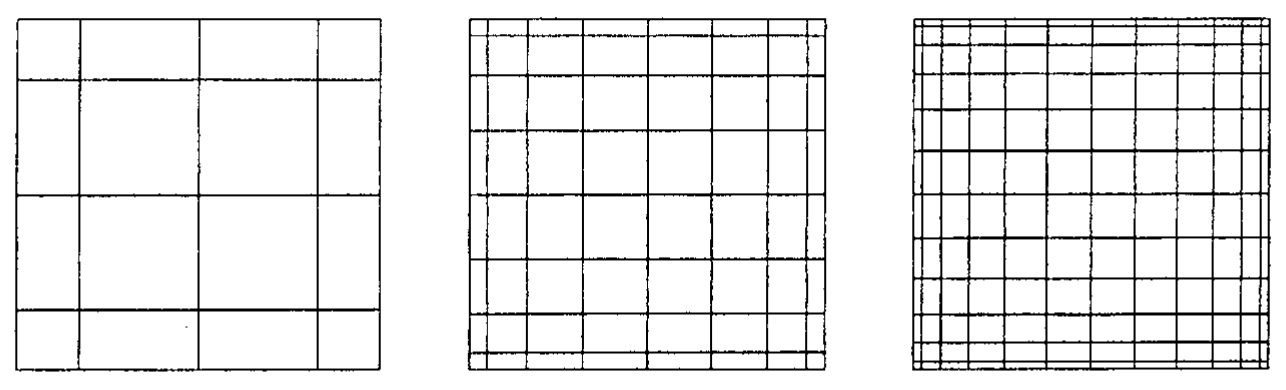
\includegraphics[width=.702\paperwidth]{images/fig-4-5-1.png}
  \caption{\(N=4,8,12\) 时的 Legendre--Gauss--Lobatto 网格}\label{fig:4.5.1}
\end{figure}

相应的离散内积为
\begin{equation}\label{eq:4.5.39}
  (u,v)_N:=\sum_{i,j=0}^N u(\boldsymbol{x}_{ij})v(\boldsymbol{x}_{ij})w_{ij},
  \qquad u,v\in C^0(\overline\Omega),
\end{equation}
并且
\SourcePage{139}
\begin{equation}\label{eq:4.5.40}
  (u,v)_N=(u,v)\qquad\text{若 }uv\in\mathbb Q_{2N-1}.
\end{equation}
由\eqref{eq:4.4.15}和\eqref{eq:4.4.16}容易得到
\begin{equation}\label{eq:4.5.41}
  \|u_N\|_0\le\|u_N\|_N\le\left(2+\frac1N\right)\|u_N\|_0
  \qquad\forall u_N\in\mathbb Q_N.
\end{equation}
对任意连续函数 \(u\),以 \(I_Nu\in\mathbb Q_N\) 表示 \(u\) 在节点 \(\{\boldsymbol{x}_{ij}\}\) 上的插值多项式,则
\begin{equation}\label{eq:4.5.42}
  I_Nu(\boldsymbol{x})=\sum_{k,m=0}^N u_{km}^*L_{km}(\boldsymbol{x}),\qquad
  u_{km}^*:=\frac{(u,L_{km})_N}{\|L_{km}\|_N^2},
\end{equation}
其中 \(\|v\|_N^2:=(v,v)_N\).也可以仿照\eqref{eq:4.4.18}将 \(u_{km}^*\) 写得更显式.

插值误差估计为
\begin{equation}\label{eq:4.5.43}
  \|u-I_Nu\|_k\le CN^{k-s}\|u\|_s,\qquad k=0,1,
\end{equation}
条件是 \(u\in H^s(\Omega)\),\(s\ge2\)(见\BookCite{bernardi-maday1992}{Bernardi 和 Maday(1992)}第 82–83 页).

\begin{note}\NumberedNote{note:4.5.1}{\heiti(多项式空间的基)}
次数不超过 \(N\) 的一元多项式空间 \(\mathbb P_N\)(\(N\ge0\))的一组基,可以取 \(L_k(\xi)\),也可以取 \(T_k(\xi)\),其中 \(k=0,\ldots,N\).

空间 \(\mathbb P_N^0:=\{p\in\mathbb P_N\mid p(-1)=p(1)=0\}\)(\(N\ge2\))的一组基可以取
\[
  \varphi_k(\xi)=L_k(\xi)-\varphi_k^*(\xi),\qquad 2\le k\le N,
\]
也可以取
\[
  \varphi_k(\xi)=T_k(\xi)-\varphi_k^*(\xi),\qquad 2\le k\le N,
\]
其中 \(k\) 为偶数时 \(\varphi_k^*(\xi)=1\),\(k\) 为奇数时 \(\varphi_k^*(\xi)=\xi\)(例如,见\BookCite{gottlieb-orszag1977}{Gottlieb 和 Orszag(1977)}).

也可以取 \((1-\xi^2)L_k'(\xi)\) 或 \((1-\xi^2)T_k'(\xi)\) 为 \(\mathbb P_N^0\) 的基,其中 \(1\le k\le N-1\).例如,以 Legendre 情形为例,利用 Sturm--Liouville 方程\eqref{eq:4.4.2},可知函数系 \((1-\xi^2)L_k'(\xi)\) 关于内积 \(\int_{-1}^1z(\xi)v(\xi)(1-\xi^2)^{-1}\,\mathrm d\xi\) 正交.

对于正方形 \([-1,1]^2\) 上的二元多项式空间 \(\mathbb Q_N\) 和 \(\mathbb Q_N^0\),将上述相应的一维基作张量积,就容易得到各自的基.\hfill\(\square\)
\end{note}

\section{补充说明}\label{sec:4.6}
\SourcePage{140}

对于三维区域 \(\Omega=(-1,1)^3\),可以按照第~\ref{sec:4.5.1}~节和第~\ref{sec:4.5.2}~节的思路构造 Chebyshev 逼近和 Legendre 逼近.前面给出的误差估计在三维情形下依然成立,而且可用相同的论证来证明(例如,见\BookCite{canuto-hussaini-quarteroni-zang1988}{Canuto、Hussaini、Quarteroni 和 Zang(1988)}以及\BookCite{bernardi-maday1992}{Bernardi 和 Maday(1992)}).

\BookCite{gottlieb-orszag1977}{Gottlieb 和 Orszag(1977)}以及\BookCite{boyd1989}{Boyd(1989)}的专著提供了处理多项式展开的许多有用工具,尤其是坐标变换、从无界区域到有界区域的映射以及物理空间与频率空间之间的变换公式.另见\BookCite{canuto-hussaini-quarteroni-zang1988}{Canuto、Hussaini、Quarteroni 和 Zang(1988)},其中给出了实现多项式变换和基于多项式的求积公式的若干程序.

谱方法最早是为逼近带周期数据的微分问题而提出的.在这些情形下,用基于三角多项式的 Fourier 展开取代 Chebyshev 和 Legendre 展开.本书不讨论 Fourier 谱方法.有兴趣的读者可参见\BookCite{gottlieb-orszag1977}{Gottlieb 和 Orszag(1977)}、\BookCite{canuto-hussaini-quarteroni-zang1988}{Canuto、Hussaini、Quarteroni 和 Zang(1988)}、\BookCite{mercier1989}{Mercier(1989)}以及\BookCite{boyd1989}{Boyd(1989)}.

关于 Sobolev 空间中多项式逼近的其他理论结果,见\BookCite{nikolskii1975}{Nikol’skiĭ(1975)}和\BookCite{canuto-hussaini-quarteroni-zang1988}{Canuto、Hussaini、Quarteroni 和 Zang(1988)}第 9 章,也可参见\BookCite{bernardi-maday1992}{Bernardi 和 Maday(1992)}及\BookCite{funaro1992}{Funaro(1992)},后两部著作还给出了关于 Laguerre 多项式和 Hermite 多项式的结果.

\chapter{Galerkin 法、配置法及其他方法}\label{ch:5}
\SourcePage{141}

本章简要介绍离散边值问题和初边值问题的几种经典方法.

我们从一个抽象边值问题出发,给出三个简单的例题.把问题改写为弱形式(或变分形式)后,介绍四类不同的空间逼近：Galerkin 法、Petrov--Galerkin 法、配置法和广义 Galerkin 法.对每一类方法,都回顾其主要的稳定性与收敛性质.

随后,讨论初边值问题的时间离散.为此,需要考察时间导数的几个基本有限差分格式,同时说明几种经典的分步法和算子分裂法.

\section{一个用作参照的抽象边值问题}\label{sec:5.1}

照例用 \(\Omega\) 表示 \(\mathbb R^d\) 中的有界区域(\(d=2,3\)),边界为 \(\partial\Omega\).考虑如下形式的边值问题：
\begin{equation}\label{eq:5.1.1}
  \begin{cases}
    Lu=f,&\text{在 }\Omega\text{ 内},\\
    Bu=0,&\text{在 }\partial\Omega^*\text{ 上},
  \end{cases}
\end{equation}
其中 \(f\) 是给定函数,\(u\) 是未知量,\(L\) 是线性微分算子,\(B\) 是仿射边界算子.这里 \(\partial\Omega^*\) 是 \(\partial\Omega\) 的一个子集,也可以是整个边界.通常,\(L\) 是空间 \(H\) 中的无界算子,其中 \(H\) 可以取为 \(L^2(\Omega)\) 或 \(L_w^2(\Omega)\).在 Chebyshev 谱逼近中,后一空间是\eqref{eq:4.5.3}引入的加权 Hilbert 空间.我们在空间 \(X\subset H\) 中寻找解 \(u\),要求 \(L\) 和 \(B\) 对 \(X\) 中的函数有定义.

一般可以把问题\eqref{eq:5.1.1}改写为弱形式(或变分形式).一方面,这种做法允许寻找弱解.弱解不必逐点满足\eqref{eq:5.1.1},这大大拓宽了可处理的物理问题的范围,\SourcePage{142}使数据不光滑的问题也能纳入其中.此外,弱形式便于构造逼近方法,例如 Galerkin 法及其推广,包括 Petrov--Galerkin 法和广义 Galerkin 法等.

在这一阶段,我们在许多地方采用简洁、启发性的论述,因为目的是说明各种方法所依据的基本思想.在后面各章中,会针对不同问题给出精确的数学框架.

形式上,将微分方程乘以适当的试验函数,再在区域上积分,就可以导出弱形式.在这一步,通常用分部积分的 Green 公式
\begin{equation}\label{eq:5.1.2}
  \int_\Omega\frac{\partial u}{\partial x_i}v\,\mathrm d\boldsymbol{x}
  =-\int_\Omega u\frac{\partial v}{\partial x_i}\,\mathrm d\boldsymbol{x}
    +\int_{\partial\Omega}uvn_i\,\mathrm d\gamma,\qquad i=1,\ldots,d,
\end{equation}
以降低对解 \(u\) 的求导阶数.这里 \(\boldsymbol{n}=(n_1,\ldots,n_d)\) 是 \(\partial\Omega\) 上的单位外法向量.

由此得到如下形式的问题：
\begin{equation}\label{eq:5.1.3}
  \text{求 }u\in W,\quad \mathcal A(u,v)=\mathcal F(v)
  \qquad\forall v\in V,
\end{equation}
其中 \(W\) 是容许解的空间,\(V\) 是试验函数空间.可以假定 \(W\) 和 \(V\) 都是 Hilbert 空间.\(\mathcal F\) 是 \(V\) 上的线性泛函,包含右端项 \(f\) 以及可能出现的非齐次边界项.最后,\(\mathcal A(\cdot,\cdot)\) 是与微分算子 \(L\) 相应的双线性形式.

\(u\) 的边界条件可以直接放进 \(W\) 的定义中,这类条件称为\emph{本质边界条件}.也可以通过适当选取双线性形式 \(\mathcal A\) 和泛函 \(\mathcal F\) 间接实现,这类条件称为\emph{自然边界条件}.

在大多数情况下,\(W=V\).无论如何,都要选取适当的空间 \(W\) 和 \(V\),使\eqref{eq:5.1.3}中的所有运算在数学上都有意义.

为了使说明不那么抽象,下面给出三个例题,后文还将详细讨论.这里仍以说明基本思想为主,严格的框架留待后文建立.

\begin{example}[(Poisson 问题)]\label{ex:5.1.1}
问题为
\begin{equation}\label{eq:5.1.4}
  \begin{cases}
    -\Delta u=f,&\text{在 }\Omega\text{ 内},\\
    u=0,&\text{在 }\partial\Omega\text{ 上},
  \end{cases}
\end{equation}
其中 \(f\) 是给定函数,\SourcePage{143}
\[
  \Delta:=\sum_{i=1}^d\frac{\partial^2}{\partial x_i^2}
\]
是 Laplace 算子.这一问题见于许多应用,将在第~\BookRef{ch:6}{6}~章讨论.

为得到其变分形式,回顾 Laplace 算子的 Green 公式：
\begin{equation}\label{eq:5.1.5}
  -\int_\Omega(\Delta u)v\,\mathrm d\boldsymbol{x}
  =\int_\Omega\nabla u\cdot\nabla v\,\mathrm d\boldsymbol{x}
    -\int_{\partial\Omega}\frac{\partial u}{\partial n}v\,\mathrm d\gamma.
\end{equation}
注意到 \(\Delta u=\operatorname{div}\nabla u\),此式可由\eqref{eq:5.1.2}得到.结合\eqref{eq:5.1.4}和\eqref{eq:5.1.5},容易看出 \(u\) 满足形如\eqref{eq:5.1.3}的问题,其中
\begin{equation}\label{eq:5.1.6}
  \begin{cases}
    W=V=H_0^1(\Omega),\\
    \mathcal A(u,v):=\displaystyle\int_\Omega\nabla u\cdot\nabla v\,\mathrm d\boldsymbol{x},\\
    \mathcal F(v):=\displaystyle\int_\Omega fv\,\mathrm d\boldsymbol{x},
  \end{cases}
\end{equation}
而 \(H_0^1(\Omega)\) 在第~\ref{sec:1.2}~节定义.
\end{example}

\begin{example}[(Stokes 问题)]\label{ex:5.1.2}
这一次求解的问题是
\begin{equation}\label{eq:5.1.7}
  \begin{cases}
    -\nu\Delta\boldsymbol{u}+\nabla p=\boldsymbol{f},&\text{在 }\Omega\text{ 内},\\
    \operatorname{div}\boldsymbol{u}=0,&\text{在 }\Omega\text{ 内},\\
    \boldsymbol{u}=\boldsymbol{0},&\text{在 }\partial\Omega\text{ 上},
  \end{cases}
\end{equation}
其中 \(\nu\) 为正常数,\(\boldsymbol{f}\) 是给定的向量函数.第~\BookRef{ch:9}{9}~章讨论这一问题,第~\BookRef{ch:10}{10}~章则在黏性不可压缩流动的 Navier--Stokes 方程框架中推导它.在这里,\(\boldsymbol{u}\) 和 \(p\) 分别表示流体的速度和压力.第一式是线性化的动量方程,第二式表达不可压缩性约束.

问题\eqref{eq:5.1.7}可写成\eqref{eq:5.1.1}的形式,只需令
\[
  u=\begin{pmatrix}\boldsymbol{u}\\p\end{pmatrix},\quad
  f=\begin{pmatrix}\boldsymbol{f}\\0\end{pmatrix},\quad
  L=\begin{pmatrix}-\nu\Delta&\nabla\\\operatorname{div}&0\end{pmatrix},\quad
  B=\begin{pmatrix}I&0\\0&0\end{pmatrix},
\]
其中 \(I\) 是恒等算子.

其变分形式可如下导出.定义
\begin{equation}\label{eq:5.1.8}
  \mathcal V=(H_0^1(\Omega))^d,\qquad
  Q=L_0^2(\Omega):=\left\{q\in L^2(\Omega)\ \middle|\ \int_\Omega q\,\mathrm d\boldsymbol{x}=0\right\}.
\end{equation}
\(\mathcal V\) 是容许速度空间,\(Q\) 是容许压力空间.要求压力平均值为零,是为了使压力唯一.对\eqref{eq:5.1.7}的第一式应用\eqref{eq:5.1.2}和\eqref{eq:5.1.5},得到
\SourcePage{144}
\[
  \nu\int_\Omega\nabla\boldsymbol{u}:\nabla\boldsymbol{v}\,\mathrm d\boldsymbol{x}
  -\int_\Omega p\operatorname{div}\boldsymbol{v}\,\mathrm d\boldsymbol{x}
  =\int_\Omega\boldsymbol{f}\cdot\boldsymbol{v}\,\mathrm d\boldsymbol{x}
  \qquad\forall\boldsymbol{v}\in\mathcal V,
\]
由第二式则得到
\[
  \int_\Omega q\operatorname{div}\boldsymbol{u}\,\mathrm d\boldsymbol{x}=0
  \qquad\forall q\in Q.
\]
因此,令
\begin{equation}\label{eq:5.1.9}
  \left\{
  \begin{aligned}
    W=V&=\mathcal V\times Q,\\
    \mathcal A(u,v)&:=\nu\int_\Omega\nabla\boldsymbol{u}:\nabla\boldsymbol{v}\,\mathrm d\boldsymbol{x}
     -\int_\Omega p\operatorname{div}\boldsymbol{v}\,\mathrm d\boldsymbol{x}
     +\int_\Omega q\operatorname{div}\boldsymbol{u}\,\mathrm d\boldsymbol{x},\\
    \mathcal F(v)&:=\int_\Omega\boldsymbol{f}\cdot\boldsymbol{v}\,\mathrm d\boldsymbol{x},
  \end{aligned}
  \right.
\end{equation}
其中 \(u=(\boldsymbol{u},p)\)、\(v=(\boldsymbol{v},q)\in V\),即可把\eqref{eq:5.1.7}改写为\eqref{eq:5.1.3}.这一推导的更多细节见第~\BookRef{ch:9}{9}~章,不过要注意函数空间的记号有所不同.
\end{example}

\begin{example}[(定常对流问题)]\label{ex:5.1.3}
设 \(\boldsymbol{a}\)、\(a_0\) 和 \(f\) 是 \(\Omega\) 上的给定函数,考虑问题
\begin{equation}\label{eq:5.1.10}
  \begin{cases}
    \boldsymbol{a}\cdot\nabla u+a_0u=f,&\text{在 }\Omega\text{ 内},\\
    u=\varphi,&\text{在 }\partial\Omega^{\mathrm{in}}\text{ 上},
  \end{cases}
\end{equation}
其中
\[
  \partial\Omega^{\mathrm{in}}
  :=\{\boldsymbol{x}\in\partial\Omega\mid\boldsymbol{a}(\boldsymbol{x})\cdot\boldsymbol{n}(\boldsymbol{x})<0\}
\]
称为\emph{流入边界},\(\varphi\) 在其上给定.随 \(\boldsymbol{a}(\boldsymbol{x})\) 取值的不同,\(\partial\Omega^{\mathrm{in}}\) 可以是空集,可以与 \(\partial\Omega\) 一致,也可以是 \(\partial\Omega\) 的真子集.\eqref{eq:5.1.10}的含时版本是流入流出型双曲问题,将在第~\BookRef{ch:14}{14}~章讨论.

\eqref{eq:5.1.10}的一种弱形式可按如下方式得到.按\eqref{eq:5.1.2}分部积分,有
\[
  \begin{aligned}
    \int_\Omega(\boldsymbol{a}\cdot\nabla u)v\,\mathrm d\boldsymbol{x}
    &=-\int_\Omega u\operatorname{div}(\boldsymbol{a}v)\,\mathrm d\boldsymbol{x}
      +\int_{\partial\Omega^{\mathrm{in}}}(\boldsymbol{a}\cdot\boldsymbol{n})\varphi v\,\mathrm d\gamma\\
    &\quad+\int_{\partial\Omega\setminus\partial\Omega^{\mathrm{in}}}
         (\boldsymbol{a}\cdot\boldsymbol{n})uv\,\mathrm d\gamma
         \qquad\forall v\in H^1(\Omega).
  \end{aligned}
\]
注意,边界条件已在分部积分过程中计入.令 \(V=H^1(\Omega)\),并取 \(W\) 为相应的输运图空间,即在 \(L^2(\Omega)\) 中要求 \(\boldsymbol{a}\cdot\nabla u\in L^2(\Omega)\),并具有使流出项有意义的迹.在系数和边界具有相应正则性的条件下,可令
\begin{equation}\label{eq:5.1.11}
  \left\{
  \begin{aligned}
    \mathcal A(u,v)&:=-\int_\Omega u\operatorname{div}(\boldsymbol{a}v)\,\mathrm d\boldsymbol{x}
      +\int_{\partial\Omega\setminus\partial\Omega^{\mathrm{in}}}
           (\boldsymbol{a}\cdot\boldsymbol{n})uv\,\mathrm d\gamma\\
      &\quad+\int_\Omega a_0uv\,\mathrm d\boldsymbol{x},\\
    \mathcal F(v)&:=\int_\Omega fv\,\mathrm d\boldsymbol{x}
      -\int_{\partial\Omega^{\mathrm{in}}}(\boldsymbol{a}\cdot\boldsymbol{n})\varphi v\,\mathrm d\gamma,
  \end{aligned}
  \right.
\end{equation}
从而将\eqref{eq:5.1.10}写成\eqref{eq:5.1.3}的形式.
\end{example}

\subsection{泛函分析的若干结果}\label{sec:5.1.1}
\SourcePage{145}

在考察\eqref{eq:5.1.3}的数值逼近之前,先给出关于解的存在性和唯一性的两个基本泛函分析定理.第一个定理针对 \(W=V\) 这一特殊情形,因而对应于问题
\begin{equation}\label{eq:5.1.12}
  \text{求 }u\in V,\quad \mathcal A(u,v)=\mathcal F(v)
  \qquad\forall v\in V.
\end{equation}

\begin{theorem}[Lax--Milgram 引理]{5.1.1}
设 \(V\) 为实 Hilbert 空间,赋有范数 \(\|\cdot\|\).设 \(\mathcal A\colon V\times V\to\mathbb R\) 是双线性形式,\(\mathcal F\colon V\to\mathbb R\) 是连续线性泛函,即 \(\mathcal F\in V'\),其中 \(V'\) 表示 \(V\) 的对偶空间.进一步假定 \(\mathcal A(\cdot,\cdot)\) 连续,即
\begin{equation}\label{eq:5.1.13}
  \exists\gamma>0:\quad |\mathcal A(w,v)|\le\gamma\|w\|\|v\|
  \qquad\forall w,v\in V,
\end{equation}
且具有强制性,即
\begin{equation}\label{eq:5.1.14}
  \exists\alpha>0:\quad\mathcal A(v,v)\ge\alpha\|v\|^2\qquad\forall v\in V.
\end{equation}
则\eqref{eq:5.1.12}存在唯一解 \(u\in V\),并且
\begin{equation}\label{eq:5.1.15}
  \|u\|\le\frac1\alpha\|\mathcal F\|_{V'}.
\end{equation}
\end{theorem}

\begin{proof}
由 Riesz 表示定理(例如,见\BookCite{yosida1974}{Yosida(1974)}第 90 页),可以写出
\[
  \mathcal F(v)=(R\mathcal F,v)_V\qquad\forall v\in V,
\]
并且对每个固定的 \(w\in V\),
\[
  \mathcal A(w,v)=(Aw,v)_V\qquad\forall v\in V.
\]
这里 \((\cdot,\cdot)_V\) 是 \(V\) 中的内积.双射 \(R\colon V'\to V\) 和 \(A\colon V\to V\) 都是连续线性算子.更确切地说,\(R\) 是等距算子,因为
\[
  \|R\mathcal F\|=\sup_{\substack{v\in V\\v\ne0}}\frac{(R\mathcal F,v)_V}{\|v\|}
     =\sup_{\substack{v\in V\\v\ne0}}\frac{\mathcal F(v)}{\|v\|}
     =\|\mathcal F\|_{V'},
\]
而且由\eqref{eq:5.1.13},
\[
  \|Aw\|=\sup_{\substack{v\in V\\v\ne0}}\frac{(Aw,v)_V}{\|v\|}
     =\sup_{\substack{v\in V\\v\ne0}}\frac{\mathcal A(w,v)}{\|v\|}
     \le\gamma\|w\|.
\]
于是,问题\eqref{eq:5.1.12}等价于：对每个 \(\mathcal F\in V'\),求唯一的 \(u\in V\),使得
\begin{equation}\label{eq:5.1.16}
  Au=R\mathcal F.
\end{equation}
\SourcePage{146}
也就是证明 \(A\) 是双射.

先证明 \(A\) 是单射.我们有
\begin{equation}\label{eq:5.1.17}
  \|v\|^2\le\frac1\alpha(Av,v)_V
    \le\frac1\alpha\|Av\|\|v\|,
\end{equation}
从而 \(\|v\|\le\|Av\|/\alpha\).由此得到唯一性.

现在证明值域 \(\mathcal R(A)\) 是闭的,且 \(\mathcal R(A)^\perp=\{0\}\).这等价于证明 \(\mathcal R(A)=V\).(若 \(S\) 是具有内积 \((\cdot,\cdot)_X\) 的 Hilbert 空间 \(X\) 的闭子空间,则其正交补 \(S^\perp\) 由满足 \((y,x)_X=0\) 对所有 \(x\in S\) 成立的 \(y\in X\) 组成.)设 \(Av_n\to w\) 于 \(V\).由\eqref{eq:5.1.17},
\[
  \|v_n-v_m\|\le\frac1\alpha\|Av_n-Av_m\|,
\]
所以 \(v_n\) 是 Cauchy 序列.设 \(v=\lim_{n\to\infty}v_n\).由 \(A\) 的连续性,\(Av=w\),因此 \(\mathcal R(A)\) 是闭的.取 \(z\in\mathcal R(A)^\perp\),则
\[
  0=(Az,z)_V=\mathcal A(z,z)\ge\alpha\|z\|^2,
\]
即 \(z=0\).

最后只需证明\eqref{eq:5.1.15}.在\eqref{eq:5.1.12}中取 \(v=u\),得到
\[
  \|u\|^2\le\frac1\alpha\mathcal A(u,u)=\frac1\alpha\mathcal F(u)
    \le\frac1\alpha\|\mathcal F\|_{V'}\|u\|,
\]
从而得到\eqref{eq:5.1.15}.\hfill\(\square\)
\end{proof}

\begin{note}\NumberedNote{note:5.1.1}{\heiti(对称情形)}
若双线性形式对称,即
\begin{equation}\label{eq:5.1.18}
  \mathcal A(w,v)=\mathcal A(v,w)\qquad\forall w,v\in V,
\end{equation}
则 \(\mathcal A(\cdot,\cdot)\) 在 \(V\) 上定义一个内积,直接应用 Riesz 表示定理便可推出\eqref{eq:5.1.12}解的存在性和唯一性.再回顾一下,在这种情形下,\eqref{eq:5.1.12}的解可看作下列最小化问题的唯一解：
\begin{equation}\label{eq:5.1.19}
  \text{求 }u\in V,\quad J(u)\le J(v)\qquad\forall v\in V,
\end{equation}
其中
\begin{equation}\label{eq:5.1.20}
  J(v):=\frac12\mathcal A(v,v)-\mathcal F(v)
\end{equation}
是一个二次泛函.\hfill\(\square\)
\end{note}

\begin{note}\NumberedNote{note:5.1.2}{\heiti(复数情形)}
若 \(V\) 是复 Hilbert 空间,就要修改对形式 \(\mathcal A(\cdot,\cdot)\) 的假设.首先,要求 \(\mathcal A\) 是半双线性的,即对第一个变量线性,并且
\[
  \mathcal A(w,c_1v_1+c_2v_2)
   =\overline c_1\mathcal A(w,v_1)+\overline c_2\mathcal A(w,v_2)
\]
\SourcePage{147}
对任意 \(w,v_1,v_2\in V\) 和 \(c_1,c_2\in\mathbb C\) 成立.这里 \(\overline c_k\) 是复数 \(c_k\) 的共轭,\(k=1,2\).相应地,\(\mathcal F\) 为连续共轭线性泛函.此外,强制性假设改为
\begin{equation}\label{eq:5.1.21}
  |\mathcal A(v,v)|\ge\alpha\|v\|^2\qquad\forall v\in V.
\end{equation}
Lax--Milgram 引理的证明基本不变.

在实数情形下,条件\eqref{eq:5.1.21}与\eqref{eq:5.1.14}只差一个整体符号.可以证明,它或者等价于对每个 \(v\in V\) 都有 \(\mathcal A(v,v)\ge\alpha\|v\|^2\),或者等价于对每个 \(v\in V\) 都有 \(-\mathcal A(v,v)\ge\alpha\|v\|^2\).也就是说,\(\mathcal A(\cdot,\cdot)\) 或 \(-\mathcal A(\cdot,\cdot)\) 必须满足\eqref{eq:5.1.14}.\hfill\(\square\)
\end{note}

在 \(W\) 与 \(V\) 不同的更一般情形下,可用下面的结果分析问题\eqref{eq:5.1.3}.这一结果是\BookCite{necas1962}{Nečas(1962)}对 Lax--Milgram 引理的推广.

\begin{theorem}[]{5.1.2}
设 \(W\) 和 \(V\) 是两个实 Hilbert 空间,范数分别为 \(\tnorm{\cdot}\) 和 \(\|\cdot\|\).设存在两个正常数 \(\alpha,\gamma\),使双线性形式 \(\mathcal A\colon W\times V\to\mathbb R\) 满足
\begin{align}
  |\mathcal A(w,v)|&\le\gamma\tnorm{w}\|v\|\qquad\forall w\in W,\ v\in V,
    \label{eq:5.1.22}\\
  \sup_{\substack{v\in V\\v\ne0}}\frac{\mathcal A(w,v)}{\|v\|}
    &\ge\alpha\tnorm{w}\qquad\forall w\in W,
    \label{eq:5.1.23}\\
  \sup_{w\in W}\mathcal A(w,v)&>0\qquad\forall v\in V,\ v\ne0.
    \label{eq:5.1.24}
\end{align}
则对任意 \(\mathcal F\in V'\),\eqref{eq:5.1.3}存在唯一解 \(u\in W\),且
\begin{equation}\label{eq:5.1.25}
  \tnorm{u}\le\frac{\|\mathcal F\|_{V'}}{\alpha}.
\end{equation}
\end{theorem}

\begin{proof}
证明与 Lax--Milgram 引理(定理~\ref{thm:5.1.1})很相似.事实上,由 Riesz 表示定理,可构造连续线性算子 \(A\colon W\to V\),使得
\begin{equation}\label{eq:5.1.26}
  \mathcal A(w,v)=(Aw,v)_V\qquad\forall v\in V
\end{equation}
对每个 \(w\in W\) 成立,其中 \((\cdot,\cdot)_V\) 表示 \(V\) 中的内积.此外,
\[
  \|Aw\|\le\gamma\tnorm{w}\qquad\forall w\in W.
\]
于是问题归结为：对任意给定的 \(\mathcal F\in V'\),求唯一的 \(u\in W\),使得
\begin{equation}\label{eq:5.1.27}
  Au=R\mathcal F.
\end{equation}
这里 \(R\colon V'\to V\) 是定理~\ref{thm:5.1.1}的证明中构造的等距算子.

\SourcePage{148}
由\eqref{eq:5.1.23}和\eqref{eq:5.1.26}立即可知,\(Aw=0\) 蕴含 \(w=0\),即 \(A\) 是单射.

此外,\(A\) 的值域 \(\mathcal R(A)\) 是闭的.事实上,若 \(Aw_n\to v\) 于 \(V\),则
\[
  \tnorm{w_n-w_m}\le\frac1\alpha
    \sup_{\substack{v_0\in V\\v_0\ne0}}
        \frac{\mathcal A(w_n-w_m,v_0)}{\|v_0\|}
    \le\frac1\alpha\|A(w_n-w_m)\|,
\]
所以 \(w_n\to w\) 于 \(W\),且 \(Aw_n\to Aw=v\) 于 \(V\).最后,若 \(z\in\mathcal R(A)^\perp\),即
\[
  (Aw,z)_V=\mathcal A(w,z)=0\qquad\forall w\in W,
\]
则由\eqref{eq:5.1.24}可知 \(z=0\),故 \(A\) 是满射.这样就证明了,对每个 \(\mathcal F\in V'\),\eqref{eq:5.1.27}存在唯一解 \(u\).

此外,
\[
  \alpha\tnorm{u}\le\sup_{\substack{v\in V\\v\ne0}}\frac{(Au,v)_V}{\|v\|}
    =\sup_{\substack{v\in V\\v\ne0}}\frac{(R\mathcal F,v)_V}{\|v\|}
    =\|\mathcal F\|_{V'},
\]
所以\eqref{eq:5.1.25}成立.\hfill\(\square\)
\end{proof}

\section{Galerkin 法}\label{sec:5.2}

现在考虑 \(W=V\) 的情形,因此所讨论的问题是\eqref{eq:5.1.12}.

设 \(h>0\) 是一个在应用中将取“小值”的参数.在有限元法中,\(h\) 是网格间距；在谱方法中,它是谱解的多项式次数的倒数,见第~\ref{ch:3}~章和第~\ref{ch:4}~章.记
\begin{equation}\label{eq:5.2.1}
  \{V_h\mid h>0\}
\end{equation}
为 \(V\) 的一族有限维子空间.假设
\begin{equation}\label{eq:5.2.2}
  \forall v\in V,\qquad
  \inf_{v_h\in V_h}\|v-v_h\|\longrightarrow0
  \quad\text{当 }h\to0\text{ 时.}
\end{equation}
\eqref{eq:5.1.12}的 Galerkin 逼近如下.给定 \(\mathcal F\in V'\),
\begin{equation}\label{eq:5.2.3}
  \text{求 }u_h\in V_h,\quad \mathcal A(u_h,v_h)=\mathcal F(v_h)
  \qquad\forall v_h\in V_h.
\end{equation}
因此,这是一种对\eqref{eq:5.1.12}的\emph{内部逼近}.从代数的角度看,设 \(\{\varphi_j\mid j=1,\ldots,N_h\}\) 是向量空间 \(V_h\) 的一组基,可以写成
\begin{equation}\label{eq:5.2.4}
  u_h(\boldsymbol{x})=\sum_{j=1}^{N_h}\xi_j\varphi_j(\boldsymbol{x}).
\end{equation}
\SourcePage{149}
由\eqref{eq:5.2.3}得到下列 \(N_h\) 阶线性方程组：
\begin{equation}\label{eq:5.2.5}
  A\boldsymbol{\xi}=\boldsymbol{F},
\end{equation}
其中 \(\boldsymbol{\xi}=(\xi_j)\)、\(\boldsymbol{F}:=(\mathcal F(\varphi_i))\),而 \(A_{ij}:=\mathcal A(\varphi_j,\varphi_i)\)(\(i,j=1,\ldots,N_h\)).矩阵 \(A\) 称为\emph{刚度矩阵}.它的性质见后面的笔记~\ref{note:5.2.2}.

对于问题\eqref{eq:5.2.3},有下列结果.

\begin{theorem}[]{5.2.1}
在定理~\ref{thm:5.1.1}的假设下,\eqref{eq:5.2.3}有唯一解 \(u_h\),而且这个解是稳定的,因为
\begin{equation}\label{eq:5.2.6}
  \|u_h\|\le\frac{\|\mathcal F\|_{V'}}{\alpha}.
\end{equation}
此外,若 \(u\) 是\eqref{eq:5.1.12}的解,则
\begin{equation}\label{eq:5.2.7}
  \|u-u_h\|\le\frac\gamma\alpha\inf_{v_h\in V_h}\|u-v_h\|.
\end{equation}
由\eqref{eq:5.2.2}可知 \(u_h\) 收敛到 \(u\).
\end{theorem}

\begin{proof}
由于 \(V_h\) 是 \(V\) 的子空间,在假设\eqref{eq:5.1.13}和\eqref{eq:5.1.14}下,可以对问题\eqref{eq:5.2.3}应用 Lax--Milgram 引理,得到 \(u_h\) 的存在性和唯一性.取 \(v_h=u_h\),由\eqref{eq:5.1.14}可得
\[
  \alpha\|u_h\|^2\le\mathcal A(u_h,u_h)=\mathcal F(u_h)
    \le\|\mathcal F\|_{V'}\|u_h\|.
\]
于是得到\eqref{eq:5.2.6}.由于 \(\|\mathcal F\|_{V'}\) 和 \(\alpha\) 都与 \(h\) 无关,这便给出了稳定性.现在将\eqref{eq:5.1.12}的试验函数限制在 \(V_h\) 中,再减去\eqref{eq:5.2.3},得到
\begin{equation}\label{eq:5.2.8}
  \mathcal A(u-u_h,v_h)=0\qquad\forall v_h\in V_h.
\end{equation}
利用\eqref{eq:5.1.13}、\eqref{eq:5.1.14},并在\eqref{eq:5.2.8}中取 \(v_h=w_h-u_h\),其中 \(w_h\in V_h\),可得
\[
  \begin{aligned}
    \alpha\|u-u_h\|^2
    &\le\mathcal A(u-u_h,u-u_h)=\mathcal A(u-u_h,u-w_h)\\
    &\le\gamma\|u-u_h\|\|u-w_h\|\qquad\forall w_h\in V_h.
  \end{aligned}
\]
由此得到\eqref{eq:5.2.7}.\hfill\(\square\)
\end{proof}

估计\eqref{eq:5.2.7}通常称为 Céa 引理.

\begin{note}\NumberedNote{note:5.2.1}{\heiti(对称情形)}
当 \(\mathcal A(\cdot,\cdot)\) 对称时,Galerkin 法称为 Ritz 法.这时,\eqref{eq:5.2.3}解的存在性和唯一性仍可由 Riesz 表示定理推出.此外,\eqref{eq:5.2.8}表明,在 \(\mathcal A\) 诱导的内积下,误差 \(u-u_h\) 与 \(V_h\) 正交.因此,\(u_h\) 是\SourcePage{150}\(u\) 关于同一内积到 \(V_h\) 的正交投影,可立即得到不等式\eqref{eq:5.2.7},而且其中的常数可改进为 \((\gamma/\alpha)^{1/2}\).\hfill\(\square\)
\end{note}

\begin{note}\NumberedNote{note:5.2.2}{\heiti(刚度矩阵 \(A\) 的性质)}
\eqref{eq:5.2.5}中定义的矩阵 \(A\) 是正定的,即对任意非零向量 \(\boldsymbol{\eta}\in\mathbb R^{N_h}\),均有 \((A\boldsymbol{\eta},\boldsymbol{\eta})>0\),其中 \((\cdot,\cdot)\) 表示 Euclid 内积.事实上,令 \(\eta_h\in V_h\) 为函数
\begin{equation}\label{eq:5.2.9}
  \eta_h(\boldsymbol{x})=\sum_{j=1}^{N_h}\eta_j\varphi_j(\boldsymbol{x}).
\end{equation}
则
\[
  (A\boldsymbol{\eta},\boldsymbol{\eta})
   =\sum_{i,j=1}^{N_h}\eta_i\mathcal A(\varphi_j,\varphi_i)\eta_j
   =\mathcal A(\eta_h,\eta_h),
\]
由\eqref{eq:5.1.14}即得结论.特别地,\(A\) 的每个特征值都具有正实部.

因此,\eqref{eq:5.2.3}解的存在性和唯一性也可以用纯代数论证证明,无需诉诸 Lax--Milgram 引理.

当双线性形式 \(\mathcal A\) 对称时,立即可知 \(A\) 也对称.\hfill\(\square\)
\end{note}

\section{Petrov--Galerkin 法}\label{sec:5.3}

这里的数值问题为
\begin{equation}\label{eq:5.3.1}
  \text{求 }u_h\in W_h,\quad
  \mathcal A_h(u_h,v_h)=\mathcal F_h(v_h)\qquad\forall v_h\in V_h,
\end{equation}
其中 \(\{W_h\mid h>0\}\) 和 \(\{V_h\mid h>0\}\) 是两族有限维空间.对每个 \(h>0\),\(W_h\ne V_h\),但 \(\dim W_h=\dim V_h=N_h\).

如果 \(\mathcal A_h\colon W_h\times V_h\to\mathbb R\) 和 \(\mathcal F_h\colon V_h\to\mathbb R\) 分别是 \(\mathcal A\) 和 \(\mathcal F\) 的适当逼近(也可与它们一致),且 \(W_h\) 是 \(W\) 的子空间,\(V_h\) 是 \(V\) 的子空间,那么可以把\eqref{eq:5.3.1}看作\eqref{eq:5.1.3}的逼近.这里,\(W\) 与 \(V\) 可以是同一个空间.

\eqref{eq:5.3.1}的代数表述如下.令 \(\{\varphi_j\mid j=1,\ldots,N_h\}\) 是 \(W_h\) 的一组基,\(\{\psi_i\mid i=1,\ldots,N_h\}\) 是 \(V_h\) 的一组基.仍按\eqref{eq:5.2.4}展开\eqref{eq:5.3.1}的解 \(u_h\),便得到下列 \(N_h\) 阶方程组：
\begin{equation}\label{eq:5.3.2}
  A\boldsymbol{\xi}=\boldsymbol{F},
\end{equation}
其中 \(\boldsymbol{\xi}=(\xi_j)\)、\(\boldsymbol{F}:=(\mathcal F_h(\psi_i))\),\(A_{ij}:=\mathcal A_h(\varphi_j,\psi_i)\).

\SourcePage{151}
对于\eqref{eq:5.3.1}的稳定性和收敛性分析,有如下由 Babuška 得到的定理(例如,见\BookCite{babuska-aziz1972}{Babuška 和 Aziz(1972)}).

\begin{theorem}[]{5.3.1}
在定理~\ref{thm:5.1.2}的假设下,再设 \(\mathcal F_h\colon V_h\to\mathbb R\) 是线性映射,\(\mathcal A_h\colon W_h\times V_h\to\mathbb R\) 是双线性形式,满足与 \(\mathcal A\) 的条件\eqref{eq:5.1.23}、\eqref{eq:5.1.24}相同的性质,其中用 \(W_h\) 代替 \(W\),用 \(V_h\) 代替 \(V\),用 \(\alpha_h\) 代替 \(\alpha\).则\eqref{eq:5.3.1}存在唯一解 \(u_h\),且
\begin{equation}\label{eq:5.3.3}
  \tnorm{u_h}\le\frac1{\alpha_h}
    \sup_{\substack{v_h\in V_h\\v_h\ne0}}\frac{\mathcal F_h(v_h)}{\|v_h\|}.
\end{equation}
进一步,若 \(u\) 是\eqref{eq:5.1.3}的解,则
\begin{equation}\label{eq:5.3.4}
  \begin{aligned}
    \tnorm{u-u_h}\le{}&
      \inf_{w_h\in W_h}\left[\left(1+\frac\gamma{\alpha_h}\right)\tnorm{u-w_h}
       +\frac1{\alpha_h}\sup_{\substack{v_h\in V_h\\v_h\ne0}}
         \frac{|\mathcal A(w_h,v_h)-\mathcal A_h(w_h,v_h)|}{\|v_h\|}\right]\\
     &+\frac1{\alpha_h}\sup_{\substack{v_h\in V_h\\v_h\ne0}}
             \frac{|\mathcal F(v_h)-\mathcal F_h(v_h)|}{\|v_h\|}.
  \end{aligned}
\end{equation}
\end{theorem}

\begin{proof}
对任意固定的 \(h\),存在性和唯一性由定理~\ref{thm:5.1.2}推出.此外,将\eqref{eq:5.1.23}用于 \(\mathcal A_h\) 的对应条件,并用\eqref{eq:5.3.1},得到\eqref{eq:5.3.3}.事实上,
\[
  \tnorm{u_h}\le\frac1{\alpha_h}\sup_{\substack{v_h\in V_h\\v_h\ne0}}
       \frac{\mathcal A_h(u_h,v_h)}{\|v_h\|}
    =\frac1{\alpha_h}\sup_{\substack{v_h\in V_h\\v_h\ne0}}
       \frac{\mathcal F_h(v_h)}{\|v_h\|}.
\]
为证明\eqref{eq:5.3.4},注意对所有 \(w_h\in W_h\) 和 \(v_h\in V_h\),有
\[
  \begin{aligned}
    \mathcal A_h(u_h-w_h,v_h)
     &=\mathcal A(u-w_h,v_h)+\mathcal A(w_h,v_h)-\mathcal A_h(w_h,v_h)\\
     &\quad+\mathcal F_h(v_h)-\mathcal F(v_h).
  \end{aligned}
\]
利用\eqref{eq:5.1.22}以及\eqref{eq:5.1.23}的离散对应式,得到
\[
  \begin{aligned}
    \alpha_h\tnorm{u_h-w_h}\le{}&\gamma\tnorm{u-w_h}\\
      &+\sup_{\substack{v_h\in V_h\\v_h\ne0}}\left\{
         \frac{|\mathcal A(w_h,v_h)-\mathcal A_h(w_h,v_h)|}{\|v_h\|}
         +\frac{|\mathcal F(v_h)-\mathcal F_h(v_h)|}{\|v_h\|}\right\}.
  \end{aligned}
\]
再用三角不等式
\[
  \tnorm{u-u_h}\le\tnorm{u-w_h}+\tnorm{u_h-w_h},
\]
便得到\eqref{eq:5.3.4}.\hfill\(\square\)
\end{proof}

\SourcePage{152}
Petrov--Galerkin 逼近的例子有通常所说的 \(\tau\) 法(例如,见\BookCite{canuto-hussaini-quarteroni-zang1988}{Canuto、Hussaini、Quarteroni 和 Zang(1988)}第 10.4 节),以及对流--扩散方程的迎风处理(见第~\BookRef{sec:8.2.2}{8.2.2}~节).

此外,Petrov--Galerkin 逼近有时可写成
\begin{equation}\label{eq:5.3.5}
  \text{求 }u_h\in W_h,\quad
  \mathcal A_h(u_h,w_h+L_hw_h)=\mathcal F_h(w_h+L_hw_h)
    \qquad\forall w_h\in W_h,
\end{equation}
其中 \(L_h\) 是按某种准则选择的、与 \(L\) 有关的适当算子.令
\[
  V_h:=\{w_h+L_hw_h\mid w_h\in W_h\},
\]
即可将问题\eqref{eq:5.3.5}写成\eqref{eq:5.3.1}的形式.在第~\BookRef{sec:14.3}{14.3}~节可以找到这类例子,其中用 GALS、SUPG 和 DWG 法逼近纯对流方程(见笔记~\BookRef{note:14.3.1}{14.3.1}).

\section{配置法}\label{sec:5.4}

配置法用于几种有限维逼近,尤其见于边界元法、有限元法和谱方法.为简明起见,这里只讨论最后一种情形,因为配置法在谱方法中的应用远比其他情形成功.

因此,可以将讨论限于区域 \(\Omega=(-1,1)^d\),\(d=2,3\),并假设所求离散解是一个关于每个坐标的次数均不超过 \(N\) 的代数多项式.此外,给定 \((N+1)^d\) 个配置点 \(\boldsymbol{x}_i\in\overline\Omega\),它们是 Gauss--Lobatto 求积公式的节点(见\eqref{eq:4.5.19}或\eqref{eq:4.5.38}).

谱配置解是一个函数 \(u_N\in\mathbb Q_N\),其中 \(\mathbb Q_N\) 是关于每个变量 \(x_i\)(\(i=1,\ldots,d\))的次数分别不超过 \(N\) 的代数多项式空间.它满足
\begin{equation}\label{eq:5.4.1}
  \begin{cases}
    L_Nu_N=f,&\text{在节点 }\boldsymbol{x}_i\in\overline\Omega\setminus\partial\Omega^*\text{ 处},\\
    B_Nu_N=0,&\text{在节点 }\boldsymbol{x}_i\in\partial\Omega^*\text{ 处},
  \end{cases}
\end{equation}
其中通常用 \(L_N\) 逼近 \(L\),做法是将各导数替换为伪谱导数,也就是在节点 \(\{\boldsymbol{x}_i\}\) 上插值得到的多项式的精确导数(见第~\ref{sec:4.3.2}~节和第~\ref{sec:4.4.2}~节).\(B_N\) 也作相应处理.

这样,就在 \(\partial\Omega^*\) 上的所有节点处施加边界条件,并在其余所有 Gauss--Lobatto 节点处施加微分方程.更确切地说,若 \(Bu=0\) 表示\SourcePage{153}自然边界条件,也可在 \(\partial\Omega^*\) 的节点处施加该边界条件与微分方程残差的适当线性组合.这样便在离散层面以自然方式施加边界条件.

我们将在第~\BookRef{sec:6.2.2}{6.2.2}~节看到,当原问题具有\eqref{eq:5.1.12}的形式时,这一做法归结为求解
\begin{equation}\label{eq:5.4.2}
  \text{求 }u_N\in V_N,\quad
   \mathcal A_N(u_N,v_N)=\mathcal F_N(v_N)\qquad\forall v_N\in V_N,
\end{equation}
其中 \(V_N=\mathbb Q_N\cap V\),而 \(\mathcal A_N\) 是对形式 \(\mathcal A\) 的逼近,其中所有积分均通过 Gauss--Lobatto 求积公式计算.右端项作同样的逼近.

\eqref{eq:5.4.2}称为谱配置法的\emph{弱形式},而\eqref{eq:5.4.1}称为\emph{强形式}.写成\eqref{eq:5.4.2}时,这一问题实际上表现为广义 Galerkin 法,因此适用下一节的稳定性和收敛性分析.

从代数的角度看,令 \(\{\psi_j\}\) 表示强形式中 \(\mathbb Q_N\) 的 Lagrange 基,即
\begin{equation}\label{eq:5.4.3}
  \psi_j\in\mathbb Q_N,\qquad \psi_j(\boldsymbol{x}_i)=\delta_{ij}
    \qquad\forall i,j=1,\ldots,(N+1)^d.
\end{equation}
令
\[
  u_N(\boldsymbol{x})=\sum_j\xi_j\psi_j(\boldsymbol{x}),\qquad
  \xi_j=u_N(\boldsymbol{x}_j),
\]
由\eqref{eq:5.4.1}可得
\begin{equation}\label{eq:5.4.4}
  \begin{cases}
    \displaystyle\sum_j(L_N\psi_j)(\boldsymbol{x}_i)\xi_j=f(\boldsymbol{x}_i),
        &\text{对所有使 \(\boldsymbol{x}_i\in\overline\Omega\setminus\partial\Omega^*\) 的 \(i\)},\\[3pt]
    \displaystyle\sum_j(B_N^{\mathrm{lin}}\psi_j)(\boldsymbol{x}_i)\xi_j
         =-(B_N0)(\boldsymbol{x}_i),
        &\text{对所有使 \(\boldsymbol{x}_i\in\partial\Omega^*\) 的 \(i\)},
  \end{cases}
\end{equation}
其中 \(B_N^{\mathrm{lin}}v:=B_Nv-B_N0\) 是仿射算子 \(B_N\) 的线性部分.若边界条件齐次,第二式右端为零.这就得到了关于 \(\boldsymbol{\xi}=(\xi_j)\) 的线性方程组,其矩阵可以用伪谱微分矩阵表示.因此,谱配置法也称为\emph{伪谱法}.

\section{广义 Galerkin 法}\label{sec:5.5}

在这种情形下,有限维问题为
\begin{equation}\label{eq:5.5.1}
  \text{求 }u_h\in V_h,\quad
  \mathcal A_h(u_h,v_h)=\mathcal F_h(v_h)\qquad\forall v_h\in V_h,
\end{equation}
其中 \(\{V_h\mid h>0\}\) 是 \(V\) 的一族有限维子空间.\(\mathcal A_h\) 和 \(\mathcal F_h\) 分别表示 \(\mathcal A\) 和 \(\mathcal F\) 的适当逼近.这是\eqref{eq:5.3.1}在允许试探空间与试验空间相同时的情形,包括配置法的\SourcePage{154}弱形式\eqref{eq:5.4.2}.不过,这里单独给出分析,因为本情形的收敛性证明有些不同.广义 Galerkin 法的其他例子包括使用数值积分的 Galerkin 有限元法(见第~\BookRef{sec:6.2.3}{6.2.3}~节),以及对流--扩散问题和 Stokes 问题的稳定化方法(见第~\BookRef{sec:8.3}{8.3}~节和第~\BookRef{sec:9.4}{9.4}~节).

回顾一下,\(\mathcal F_h(\cdot)\) 是定义在 \(V_h\) 上的线性泛函,\(\mathcal A_h(\cdot,\cdot)\) 是定义在 \(V_h\times V_h\) 上的双线性形式.将它们作用于 \(V\) 的元素时,未必有意义.事实上,\(\mathcal A_h\) 和 \(\mathcal F_h\) 往往涉及 \(u_h\) 或其导数的点值,而 \(V\) 中函数未必有这样的点值.例如,上面讨论的三个例题就都无法保证所需的点值有定义.

下述结果称为 Strang 第一引理.

\begin{theorem}[]{5.5.1}
在定理~\ref{thm:5.1.1}的假设下,再设 \(\mathcal F_h(\cdot)\) 是线性映射,双线性形式 \(\mathcal A_h(\cdot,\cdot)\) 在 \(V_h\times V_h\) 上一致强制.这意味着存在 \(\alpha^*>0\),使得对所有 \(h>0\),
\begin{equation}\label{eq:5.5.2}
  \mathcal A_h(v_h,v_h)\ge\alpha^*\|v_h\|^2\qquad\forall v_h\in V_h.
\end{equation}
则\eqref{eq:5.5.1}存在唯一解 \(u_h\),且
\begin{equation}\label{eq:5.5.3}
  \|u_h\|\le\frac1{\alpha^*}\sup_{\substack{v_h\in V_h\\v_h\ne0}}
                \frac{\mathcal F_h(v_h)}{\|v_h\|}.
\end{equation}
若 \(u\) 是\eqref{eq:5.1.12}的解,则
\begin{equation}\label{eq:5.5.4}
  \begin{aligned}
    \|u-u_h\|\le{}&
      \inf_{w_h\in V_h}\left[\left(1+\frac\gamma{\alpha^*}\right)\|u-w_h\|
        +\frac1{\alpha^*}\sup_{\substack{v_h\in V_h\\v_h\ne0}}
           \frac{|\mathcal A(w_h,v_h)-\mathcal A_h(w_h,v_h)|}{\|v_h\|}\right]\\
    &+\frac1{\alpha^*}\sup_{\substack{v_h\in V_h\\v_h\ne0}}
          \frac{|\mathcal F(v_h)-\mathcal F_h(v_h)|}{\|v_h\|}.
  \end{aligned}
\end{equation}
\end{theorem}

\begin{proof}
与定理~\ref{thm:5.3.1}的证明类似,由于\eqref{eq:5.5.2}成立,Lax--Milgram 引理给出存在性、唯一性和不等式\eqref{eq:5.5.3}.虽然\eqref{eq:5.5.4}的证明与\eqref{eq:5.3.4}的证明相差不大,为便于阅读,仍写在下面.

取 \(V_h\) 中任意元素 \(w_h\),令 \(\sigma_h:=u_h-w_h\).由\eqref{eq:5.5.2},
\[
  \begin{aligned}
    \alpha^*\|\sigma_h\|^2&\le\mathcal A_h(\sigma_h,\sigma_h)\\
      &=\mathcal A(u-w_h,\sigma_h)+\mathcal A(w_h,\sigma_h)
         -\mathcal A_h(w_h,\sigma_h)+\mathcal F_h(\sigma_h)-\mathcal F(\sigma_h).
  \end{aligned}
\]
\SourcePage{155}
设 \(\sigma_h\ne0\).由\eqref{eq:5.1.13},
\[
  \begin{aligned}
    \alpha^*\|\sigma_h\|
    &\le\gamma\|u-w_h\|
      +\frac{|\mathcal A(w_h,\sigma_h)-\mathcal A_h(w_h,\sigma_h)|}{\|\sigma_h\|}
      +\frac{|\mathcal F_h(\sigma_h)-\mathcal F(\sigma_h)|}{\|\sigma_h\|}\\
    &\le\gamma\|u-w_h\|+
       \sup_{\substack{v_h\in V_h\\v_h\ne0}}
          \frac{|\mathcal A(w_h,v_h)-\mathcal A_h(w_h,v_h)|}{\|v_h\|}\\
    &\quad+\sup_{\substack{v_h\in V_h\\v_h\ne0}}
        \frac{|\mathcal F_h(v_h)-\mathcal F(v_h)|}{\|v_h\|}.
  \end{aligned}
\]
当 \(\sigma_h=0\) 时,最后的不等式显然也成立.将它与三角不等式
\(\|u-u_h\|\le\|u-w_h\|+\|\sigma_h\|\) 结合,再对 \(w_h\in V_h\) 取下确界,就得到所需结果.\hfill\(\square\)
\end{proof}

下列结果也很有用.

\begin{proposition}[]{5.5.1}
在定理~\ref{thm:5.5.1}的假设下,再设双线性形式 \(\mathcal A_h(\cdot,\cdot)\) 在 \((u,v_h)\) 上有定义,其中 \(u\) 是\eqref{eq:5.1.12}的解,\(v_h\in V_h\).并且,对某个适当的 \(\gamma^*>0\),
\begin{equation}\label{eq:5.5.5}
  |\mathcal A_h(u-w_h,v_h)|\le\gamma^*\|u-w_h\|\|v_h\|
    \qquad\forall w_h,v_h\in V_h,
\end{equation}
此估计对 \(h>0\) 一致成立.则有如下收敛估计：
\begin{equation}\label{eq:5.5.6}
  \begin{aligned}
    \|u-u_h\|\le{}&\left(1+\frac{\gamma^*}{\alpha^*}\right)
                    \inf_{w_h\in V_h}\|u-w_h\|\\
      &+\frac1{\alpha^*}\sup_{\substack{v_h\in V_h\\v_h\ne0}}
          \frac{|\mathcal A_h(u,v_h)-\mathcal F_h(v_h)|}{\|v_h\|}.
  \end{aligned}
\end{equation}
\end{proposition}

\begin{proof}
设 \(w_h\) 是 \(V_h\) 中的任意元素.可以写成
\[
  \begin{aligned}
    \mathcal A_h(u_h-w_h,u_h-w_h)
    &=\mathcal A_h(u-w_h,u_h-w_h)\\
    &\quad+\mathcal F_h(u_h-w_h)-\mathcal A_h(u,u_h-w_h).
  \end{aligned}
\]
由\eqref{eq:5.5.2}和\eqref{eq:5.5.5}得到
\[
  \|u_h-w_h\|\le\frac{\gamma^*}{\alpha^*}\|u-w_h\|
    +\frac1{\alpha^*}\sup_{\substack{v_h\in V_h\\v_h\ne0}}
        \frac{|\mathcal F_h(v_h)-\mathcal A_h(u,v_h)|}{\|v_h\|}.
\]
由三角不等式立即得到\eqref{eq:5.5.6}.\hfill\(\square\)
\end{proof}

从代数的角度看,若按\eqref{eq:5.2.4}展开 \(u_h\),则问题\eqref{eq:5.5.1}给出一个形如\eqref{eq:5.2.5}的线性方程组,其中 \(\mathcal F(\cdot)\) 和 \(\mathcal A(\cdot,\cdot)\) \SourcePage{156}分别换成 \(\mathcal F_h(\cdot)\) 和 \(\mathcal A_h(\cdot,\cdot)\).强制性假设\eqref{eq:5.5.2}保证 \(A\) 是正定矩阵.若 \(\mathcal A_h(\cdot,\cdot)\) 是对称形式,则 \(A\) 也对称.

\begin{note}\NumberedNote{note:5.5.1}{\heiti(非协调逼近)}
\eqref{eq:5.5.1}的一个特殊情形是 \(V_h\) 并非 \(V\) 的子空间,因而双线性形式 \(\mathcal A\) 未必在 \(V_h\times V_h\) 上有定义.假设在 \(V+V_h\) 上定义了范数 \(\|\cdot\|_h\) 和近似双线性形式 \(\mathcal A_h(\cdot,\cdot)\),并在 \(V_h\) 上定义了近似线性泛函 \(\mathcal F_h(\cdot)\).进一步要求存在常数 \(\alpha^*,\gamma^*>0\),使得对每个 \(h>0\),
\[
  \begin{aligned}
    \mathcal A_h(v_h,v_h)&\ge\alpha^*\|v_h\|_h^2
      &&\forall v_h\in V_h,\\
    |\mathcal A_h(w,v_h)|&\le\gamma^*\|w\|_h\|v_h\|_h
      &&\forall w\in V+V_h,\quad v_h\in V_h.
  \end{aligned}
\]
由所谓的 Strang 第二引理,得到下列误差估计：
\[
  \|u-u_h\|_h\le
     \left(1+\frac{\gamma^*}{\alpha^*}\right)\inf_{w_h\in V_h}\|u-w_h\|_h
    +\frac1{\alpha^*}\sup_{\substack{v_h\in V_h\\v_h\ne0}}
          \frac{|\mathcal A_h(u,v_h)-\mathcal F_h(v_h)|}{\|v_h\|_h}.
\]
证明与命题~\ref{pro:5.5.1}非常相似.另见\BookCite{ciarlet1991}{Ciarlet(1991)}第 212–213 页.\hfill\(\square\)
\end{note}

\figref{fig:5.5.1}示意了前面各节给出的各种表述.图中 \(\overline\Omega_h\) 和 \(\partial\Omega_h^*\) 分别表示 \(\overline\Omega\) 与 \(\partial\Omega^*\) 中的配置节点集.

\begin{figure}[htbp]
  \centering
  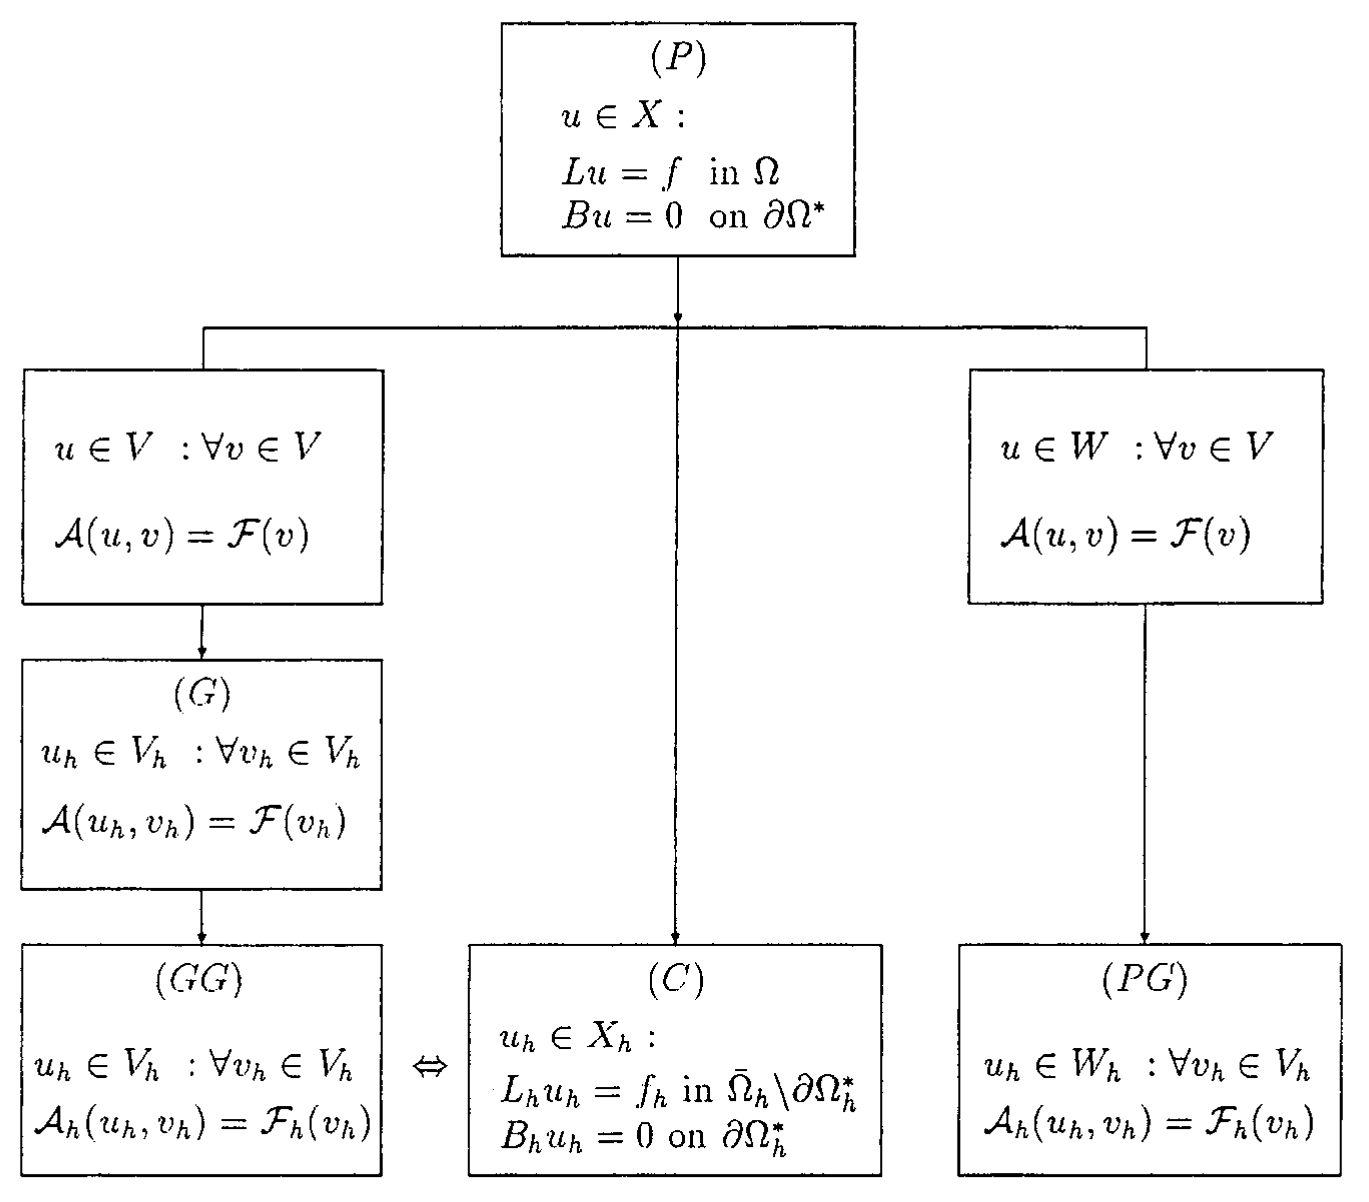
\includegraphics[width=.747\paperwidth]{images/fig-5-5-1.png}
  \caption{边值问题(P)的 Galerkin 逼近(G)、Petrov--Galerkin 逼近(PG)、广义 Galerkin 逼近(GG)和配置逼近(C)}\label{fig:5.5.1}
\end{figure}

\section{含时问题的时间推进方法}\label{sec:5.6}

本节讨论初边值问题的时间离散.这里仅作简要介绍,使读者对处理这一问题的几种方法有初步认识.本书\BookRef{part:3}{第三部分}将针对多类具体问题作详细讨论.

沿用第~\ref{sec:5.1}~节的抽象框架,现在定义下列问题：
\begin{equation}\label{eq:5.6.1}
  \begin{cases}
    \dfrac{\partial u}{\partial t}+Lu=f,&\text{在 }Q_T:=(0,T)\times\Omega\text{ 内},\\[2pt]
    Bu=0,&\text{在 }\Sigma_T^*:=(0,T)\times\partial\Omega^*\text{ 上},\\
    u=u_0,&\text{在 }\Omega\text{ 内,}t=0.
  \end{cases}
\end{equation}
\SourcePage{157}
这里 \(T>0\) 是给定的终止时刻,\(\partial/\partial t\) 表示对时间求导.未知量 \(u\) 和右端项 \(f\) 是 \(t\in(0,T)\) 与 \(\boldsymbol{x}\in\Omega\) 的函数,\(u_0=u_0(\boldsymbol{x})\) 是给定的初始数据.微分算子 \(L\) 和边界算子 \(B\) 现在可以依赖于 \(t\).

当 \(u\) 为向量值函数时,未必需要对它的每个分量作时间求导.下面介绍的 Stokes 问题便是一个例子.这类初边值问题称为\emph{微分代数方程}(见\BookCite{brenan-campbell-petzold1989}{Brenan、Campbell 和 Petzold(1989)}).

我们不讨论保证\eqref{eq:5.6.1}解的存在性和唯一性的一般假设.不过,可以假定上述问题能够写成弱形式.为此,假定存在三个 Hilbert 空间 \(V,W,H\),使得 \(W\) 和 \(V\) 都连续且稠密地嵌入 \(H\).除非另有说明,取 \(H=L^2(\Omega)\).\(H\) 中的内积记为 \((\cdot,\cdot)\).假定\SourcePage{158}\(u_0\in H\),\(f\in L^2(0,T;H)\).此外,假定存在 \(W\times V\) 上的连续双线性形式 \(\mathcal A(\cdot,\cdot)\).

\eqref{eq:5.6.1}的弱形式为：求 \(u\in L^2(0,T;W)\cap C^0([0,T];H)\)(这些空间的定义见第~\ref{sec:1.2}~节),使
\begin{equation}\label{eq:5.6.2}
  \frac{\mathrm d}{\mathrm dt}(u(t),v)+\mathcal A(u(t),v)
    =\mathcal F(t,v)\qquad\forall v\in V,
\end{equation}
并且 \(t=0\) 时 \(u=u_0\).对于微分代数系统,其中的时间导数及相应的时间连续性只涉及有时间导数的分量.右端项简记 \((f(t),v)\) 与非齐次边界条件可能产生的附加项之和.方程\eqref{eq:5.6.2}应按 \((0,T)\) 上的分布意义理解.在前述数据假设下,其中的运算都有意义.

下面给出三个例题,分别是第~\ref{sec:5.1}~节中三个例题的非定常版本.

\begin{example}[(热方程)]\label{ex:5.6.1}
考虑问题
\begin{equation}\label{eq:5.6.3}
  \begin{cases}
    \dfrac{\partial u}{\partial t}-\Delta u=f,&\text{在 }Q_T\text{ 内},\\[2pt]
    u=0,&\text{在 }\Sigma_T:=(0,T)\times\partial\Omega\text{ 上},\\
    u=u_0,&\text{在 }\Omega\text{ 内,}t=0.
  \end{cases}
\end{equation}
第~\BookRef{ch:11}{11}~章将详细讨论这个问题.它描述在外部热源 \(f\) 的作用下,\(\Omega\) 内各向同性均匀介质的温度 \(u\) 随时间的演化,其中 \(u_0\) 是初始温度.

其弱形式为：求 \(u\colon Q_T\to\mathbb R\),使 \(u(t,\cdot)\in H_0^1(\Omega)\),且
\begin{equation}\label{eq:5.6.4}
  \begin{aligned}
    &\int_\Omega\frac{\partial u}{\partial t}(t,\boldsymbol{x})v(\boldsymbol{x})\,\mathrm d\boldsymbol{x}
      +\int_\Omega\nabla u(t,\boldsymbol{x})\cdot\nabla v(\boldsymbol{x})\,\mathrm d\boldsymbol{x}\\
    &\qquad=\int_\Omega f(t,\boldsymbol{x})v(\boldsymbol{x})\,\mathrm d\boldsymbol{x}
      \qquad\forall v\in H_0^1(\Omega)
  \end{aligned}
\end{equation}
对几乎每个 \(t\in(0,T)\) 成立,并且 \(t=0\) 时 \(u=u_0\).因此,这是\eqref{eq:5.6.2}的一个特例,相应的记号见\eqref{eq:5.1.6}.
\end{example}

\begin{example}[(非定常 Stokes 问题)]\label{ex:5.6.2}
问题\eqref{eq:5.1.7}的含时版本为
\begin{equation}\label{eq:5.6.5}
  \begin{cases}
    \dfrac{\partial\boldsymbol{u}}{\partial t}-\nu\Delta\boldsymbol{u}+\nabla p
      =\boldsymbol{f},&\text{在 }Q_T\text{ 内},\\[2pt]
    \operatorname{div}\boldsymbol{u}=0,&\text{在 }Q_T\text{ 内},\\
    \boldsymbol{u}=\boldsymbol{0},&\text{在 }\Sigma_T\text{ 上},\\
    \boldsymbol{u}=\boldsymbol{u}_0,&\text{在 }\Omega\text{ 内,}t=0.
  \end{cases}
\end{equation}
\SourcePage{159}
这些方程描述 \(\Omega\) 内黏性不可压缩流体的非定常运动.这里假定流动缓慢,外力的体积密度为 \(\boldsymbol{f}\),初始速度为 \(\boldsymbol{u}_0\).第~\BookRef{ch:13}{13}~章将在含时 Navier--Stokes 方程的框架中推导这些方程.

\eqref{eq:5.6.5}的弱形式为：求 \(\boldsymbol{u}\colon Q_T\to\mathbb R^d\) 和 \(p\colon Q_T\to\mathbb R\),使得 \(\boldsymbol{u}(t,\cdot)\in(H_0^1(\Omega))^d\)、\(p(t,\cdot)\in L_0^2(\Omega)\),且
\begin{equation}\label{eq:5.6.6}
  \left\{
  \begin{aligned}
    &\int_\Omega \frac{\partial\boldsymbol{u}}{\partial t}(t,\boldsymbol{x})\cdot
           \boldsymbol{v}(\boldsymbol{x})\,\mathrm d\boldsymbol{x}
     +\nu\int_\Omega\nabla\boldsymbol{u}(t,\boldsymbol{x}):\nabla\boldsymbol{v}(\boldsymbol{x})\,\mathrm d\boldsymbol{x}\\
    &\qquad-\int_\Omega p(t,\boldsymbol{x})\operatorname{div}\boldsymbol{v}(\boldsymbol{x})\,\mathrm d\boldsymbol{x}\\
    &\qquad=\int_\Omega\boldsymbol{f}(t,\boldsymbol{x})\cdot\boldsymbol{v}(\boldsymbol{x})\,\mathrm d\boldsymbol{x}
             \qquad\forall\boldsymbol{v}\in(H_0^1(\Omega))^d,\\[3pt]
    &\int_\Omega q(\boldsymbol{x})\operatorname{div}\boldsymbol{u}(t,\boldsymbol{x})\,\mathrm d\boldsymbol{x}=0
             \qquad\forall q\in L_0^2(\Omega)
  \end{aligned}
  \right.
\end{equation}
对几乎每个 \(t\in(0,T)\) 成立,并且 \(t=0\) 时 \(\boldsymbol{u}=\boldsymbol{u}_0\).采用\eqref{eq:5.1.9}的记号,并只对速度分量求时间导数,又可将\eqref{eq:5.6.6}写成抽象形式\eqref{eq:5.6.2}.
\end{example}

\begin{example}[(线性输运问题)]\label{ex:5.6.3}
采用\eqref{eq:5.1.10}中的记号,输运方程的初边值问题为(另见第~\BookRef{ch:14}{14}~章)
\begin{equation}\label{eq:5.6.7}
  \begin{cases}
    \dfrac{\partial u}{\partial t}+\boldsymbol{a}\cdot\nabla u=f,
      &\text{在 }Q_T\text{ 内},\\[2pt]
    u=\varphi,&\text{在 }\Sigma_T^{\mathrm{in}}:=(0,T)\times\partial\Omega^{\mathrm{in}}\text{ 上},\\
    u=u_0,&\text{在 }\Omega\text{ 内,}t=0.
  \end{cases}
\end{equation}
这些方程描述量 \(u\) 的输运,其在任意点 \(\boldsymbol{x}\) 的传播速度由向量函数 \(\boldsymbol{a}\) 给出.为简便起见,可假定 \(\boldsymbol{a}\) 光滑且不依赖于 \(t\),这样流入边界 \(\partial\Omega^{\mathrm{in}}\) 不随时间变化.

\eqref{eq:5.6.7}的弱形式为：求 \(u\colon Q_T\to\mathbb R\),使 \(u(t,\cdot)\in L^2(\Omega)\),具有相应的流出迹,且
\begin{equation}\label{eq:5.6.8}
  \begin{aligned}
    &\int_\Omega\frac{\partial u}{\partial t}(t,\boldsymbol{x})v(\boldsymbol{x})\,\mathrm d\boldsymbol{x}
    -\int_\Omega u(t,\boldsymbol{x})\operatorname{div}(\boldsymbol{a}v)(\boldsymbol{x})\,\mathrm d\boldsymbol{x}\\
    &\quad+\int_{\partial\Omega\setminus\partial\Omega^{\mathrm{in}}}
      (\boldsymbol{a}\cdot\boldsymbol{n})(\boldsymbol{x})u(t,\boldsymbol{x})v(\boldsymbol{x})\,\mathrm d\gamma\\
    &=\int_\Omega f(t,\boldsymbol{x})v(\boldsymbol{x})\,\mathrm d\boldsymbol{x}
      -\int_{\partial\Omega^{\mathrm{in}}}(\boldsymbol{a}\cdot\boldsymbol{n})(\boldsymbol{x})
           \varphi(t,\boldsymbol{x})v(\boldsymbol{x})\,\mathrm d\gamma
     \qquad\forall v\in H^1(\Omega)
  \end{aligned}
\end{equation}
对几乎每个 \(t\in(0,T)\) 成立,并且 \(t=0\) 时 \(u=u_0\).由\eqref{eq:5.1.11}可见,这也是\eqref{eq:5.6.2}的一个例子.
\end{example}

\subsection{半离散逼近}\label{sec:5.6.1}
\SourcePage{160}

抽象问题\eqref{eq:5.6.2}需要对时间和空间两个变量作离散.

空间离散可以按定常问题的做法进行.例如,将\eqref{eq:5.2.3}的方法推广到\eqref{eq:5.6.2},便得到其 Galerkin 逼近.所得问题为：对每个 \(t\in[0,T]\),求 \(u_h(t,\cdot)\in V_h\subset V\),使得
\begin{equation}\label{eq:5.6.9}
  \frac{\mathrm d}{\mathrm dt}(u_h(t),v_h)+\mathcal A(u_h(t),v_h)
  =\mathcal F(t,v_h)\qquad\forall v_h\in V_h,\quad t\in(0,T),
\end{equation}
且 \(u_h(0)=u_{0,h}\),其中 \(u_{0,h}\) 是 \(V_h\) 中用来逼近初值 \(u_0\) 的适当元素.(通常取 \(u_0\) 的插值,或取它关于 \(L^2(\Omega)\) 内积或 \(V\) 内积的投影作为初值.)

类似地,也可引入基于 Petrov--Galerkin 法、广义 Galerkin 法或配置法的其他逼近.

问题\eqref{eq:5.6.9}常称为\eqref{eq:5.6.2}的\emph{半离散逼近},也称\emph{时间连续逼近}.令
\begin{equation}\label{eq:5.6.10}
  u_h(t,\boldsymbol{x})=\sum_{j=1}^{N_h}\xi_j(t)\varphi_j(\boldsymbol{x})\quad(t\ge0),
  \qquad
  u_{0,h}(\boldsymbol{x})=\sum_{j=1}^{N_h}\xi_{0,j}\varphi_j(\boldsymbol{x}),
\end{equation}
其中 \(\{\varphi_j\}\) 仍表示 \(V_h\) 的一组基.容易看出,\eqref{eq:5.6.9}给出关于未知向量 \(\boldsymbol{\xi}(t)\) 的常微分方程组：
\begin{equation}\label{eq:5.6.11}
  M\frac{\mathrm d\boldsymbol{\xi}(t)}{\mathrm dt}+A\boldsymbol{\xi}(t)
    =\boldsymbol{F}(t),\qquad \boldsymbol{\xi}(0)=\boldsymbol{\xi}_0.
\end{equation}
对每个 \(t\ge0\),\(\boldsymbol{\xi}(t)=(\xi_j(t))\),\(\boldsymbol{F}(t):=(\mathcal F(t,\varphi_i))\).此外,\(\boldsymbol{\xi}_0=(\xi_{0,j})\),且
\begin{equation}\label{eq:5.6.12}
  M_{ij}:=(\varphi_i,\varphi_j),\qquad
  A_{ij}:=\mathcal A(\varphi_j,\varphi_i),\qquad i,j=1,\ldots,N_h.
\end{equation}
刚度矩阵 \(A\) 与定常情形中引入的矩阵相同,见\eqref{eq:5.2.5}.若算子 \(L\) 不依赖于 \(t\),则 \(A\) 也不依赖于 \(t\).为便于论述,本节始终作此假设.对称正定矩阵 \(M\) 始终与 \(t\) 无关,称为\emph{质量矩阵}.对微分代数问题,相应质量矩阵在没有时间导数的分量上为零,因此不一定正定.

\subsection{全离散逼近}\label{sec:5.6.2}

\eqref{eq:5.6.9}的时间离散有多种做法.首先将时间区间 \([0,T]\) 分为 \(\mathcal N\) 个长度为 \(\Delta t=T/\mathcal N\) 的子区间 \([t_n,t_{n+1}]\),其中 \(t_0=0\),\(t_{\mathcal N}=T\).然后,在每个时刻 \(t_n\) 寻求 \(u(t_n)\) 的近似,以 \(u_h^n\) 记\SourcePage{161}相应的有限维函数.特别地,\(u_h^0\) 是 \(u_0\) 的一个适当近似.将问题\eqref{eq:5.6.9}完全离散化的经典做法,是用有限差分格式离散时间导数.这种格式用由 Taylor 展开公式得到的差商代替导数.下面通过常微分方程的 Cauchy 问题说明基本思想：
\begin{equation}\label{eq:5.6.13}
  \begin{cases}
    \dfrac{\mathrm dy}{\mathrm dt}(t)=\psi(t,y(t)),&0<t<T,\\
    y(0)=y_0,
  \end{cases}
\end{equation}
其中 \(\psi\colon[0,T]\times\mathbb R\to\mathbb R\) 是连续函数,且关于 \(y\) 满足对 \(t\in[0,T]\) 一致的 Lipschitz 条件.

在许多可能的有限差分格式中,先说明简单的 \(\theta\)-格式(\(0\le\theta\le1\)).按这一格式,上述问题由下式代替：
\begin{equation}\label{eq:5.6.14}
  \frac{y^{n+1}-y^n}{\Delta t}
    =\theta\psi(t_{n+1},y^{n+1})+(1-\theta)\psi(t_n,y^n),
\end{equation}
其中 \(n=0,\ldots,\mathcal N-1\),\(y^0=y_0\),\(y^n\) 逼近 \(y(t_n)\).

对\eqref{eq:5.6.9}应用 \(\theta\)-格式,得到
\begin{equation}\label{eq:5.6.15}
  \begin{aligned}
    &\frac1{\Delta t}(u_h^{n+1}-u_h^n,v_h)
     +\mathcal A(\theta u_h^{n+1}+(1-\theta)u_h^n,v_h)\\
    &\qquad=\theta\mathcal F(t_{n+1},v_h)+(1-\theta)\mathcal F(t_n,v_h)
            \qquad\forall v_h\in V_h,
  \end{aligned}
\end{equation}
其中 \(n=0,\ldots,\mathcal N-1\),\(u_h^0=u_{0,h}\).两个极端情形 \(\theta=0\) 和 \(\theta=1\) 分别给出熟知的前向 Euler 法和后向 Euler 法,它们关于时间步长 \(\Delta t\) 都是一阶精度.对应于 \(\theta=1/2\) 的格式称为 Crank--Nicolson 格式,在适当的光滑性条件下具有二阶精度.

两步法也能给出其他二阶格式.这类方法涉及 \(t_{n+1}\)、\(t_n\) 和 \(t_{n-1}\) 三个时刻.第一个例子是二阶 Adams--Bashforth 法：
\begin{equation}\label{eq:5.6.16}
  \frac{y^{n+1}-y^n}{\Delta t}
   =\frac32\psi(t_n,y^n)-\frac12\psi(t_{n-1},y^{n-1}),
   \qquad n=1,\ldots,\mathcal N-1.
\end{equation}
另一个例子是二阶后向差分法：
\begin{equation}\label{eq:5.6.17}
  \frac{3y^{n+1}-4y^n+y^{n-1}}{2\Delta t}=\psi(t_{n+1},y^{n+1}),
    \qquad n=1,\ldots,\mathcal N-1.
\end{equation}
两种格式都需要先求 \(y^1\),而且这一步的初始计算也必须具有二阶精度.将\eqref{eq:5.6.16}和\eqref{eq:5.6.17}用于\eqref{eq:5.6.9}的离散是直接的.

\SourcePage{162}
如果 \(u\) 及其直至 \(p+1\) 阶的时间导数连续,从形式上可以用 Taylor 公式达到 \(p\) 阶精度.

这里先指出,\eqref{eq:5.6.15}的代数形式为
\begin{equation}\label{eq:5.6.18}
  M\boldsymbol{\xi}^{n+1}+\theta\Delta t\,A\boldsymbol{\xi}^{n+1}=\boldsymbol{\eta}^{n+1},
    \qquad n=0,\ldots,\mathcal N-1,
\end{equation}
其中
\[
  \boldsymbol{\eta}^{n+1}:=\theta\Delta t\,\boldsymbol{F}(t_{n+1})
    +(1-\theta)\Delta t\,\boldsymbol{F}(t_n)
    +M\boldsymbol{\xi}^n+(\theta-1)\Delta t\,A\boldsymbol{\xi}^n,
\]
且 \(\boldsymbol{\xi}^0=\boldsymbol{\xi}_0\)(记号见\eqref{eq:5.6.10}–\eqref{eq:5.6.12}).如果先将有限差分格式用于\eqref{eq:5.6.2},再对所得的每一步定常问题作 Galerkin 空间逼近,也会得到相同的代数方程组.

当 \(\theta=0\) 时,除去对质量矩阵 \(M\) 的“求逆”,上述格式是显式的.如果 \(M\) 不是对角矩阵,常用质量集中把它变成对角形式,见第~\BookRef{sec:11.4}{11.4}~节.对于 \(\theta\) 的其他取值,\eqref{eq:5.6.18}都以隐式方式确定 \(\boldsymbol{\xi}^{n+1}\).类似地,\eqref{eq:5.6.16}是显式的,而\eqref{eq:5.6.17}是隐式的.

从计算的角度看,显式方法比隐式方法容易实现.其缺点是,显式方法一般只有\emph{条件稳定性}.对典型离散问题,时间步长 \(\Delta t\) 必须相对于 \(M^{-1}A\) 的最大特征值模的倒数足够小,因而也必须随空间尺度 \(h\) 取足够小的值.相反,某些隐式方法可以是\emph{无条件稳定的}.在这种情况下,\(\Delta t\) 的选取只由精度要求决定.

本书\BookRef{part:3}{第三部分}将针对所考虑的各类含时问题,具体说明这里提到的\emph{时间稳定性}概念.这里先作定性描述.对于 Cauchy 问题
\begin{equation}\label{eq:5.6.19}
  \begin{cases}
    \dfrac{\mathrm d\boldsymbol{\eta}}{\mathrm dt}(t)=B\boldsymbol{\eta}(t),
      &0<t<\infty,\\
    \boldsymbol{\eta}(0)=\boldsymbol{\eta}_0,
  \end{cases}
\end{equation}
其中 \(B\) 是给定的 \(m\) 阶矩阵,若存在与 \(\Delta t\) 无关的正常数 \(C,\lambda,\delta\),使得对所有 \(0<\Delta t\le\delta\),都有
\begin{equation}\label{eq:5.6.20}
  |\boldsymbol{\eta}^n|\le Ce^{\lambda t_n}|\boldsymbol{\eta}_0|,\qquad n\ge0,
\end{equation}
则称该方法稳定.这里 \(\boldsymbol{\eta}^n\) 是时刻 \(t_n=n\Delta t\) 的计算解,\(|\cdot|\) 是 \(\mathbb R^m\) 中的某个向量范数.

对于解 \(\boldsymbol{\eta}(t)\) 在所有 \(t>0\) 都有界的问题,\eqref{eq:5.6.20}允许的指数增长可能并不合适.这时,对时间离散方法提出\emph{绝对稳定性}要求更为恰当.这个概念定义如下.考虑标量\SourcePage{163}模型问题\eqref{eq:5.6.13},其中 \(\psi(t,y(t))=\mu y(t)\),\(\mu\in\mathbb C\).对给定的 \(\mu\Delta t\),若数值方法产生的近似解 \(y^n\) 在 \(n\to\infty\) 时趋于零,就称该方法对于这个 \(\mu\Delta t\) 是绝对稳定的.使方法绝对稳定的所有 \(\mu\Delta t\) 构成的集合称为\emph{绝对稳定域}.如果绝对稳定域包含 \(\{z\in\mathbb C\mid\operatorname{Re}z<0\}\),则称该方法为 \(A\)-稳定.容易证明,\(\theta\ge1/2\) 时,\(\theta\)-格式是 \(A\)-稳定的(例如,见\BookCite{lambert1991}{Lambert(1991)}第 244 页).

如果将\eqref{eq:5.6.19}换成半离散问题\eqref{eq:5.6.9},并取 \(\mathcal F(\cdot,\cdot)=0\)、\(T=\infty\),则当对所有 \(0<\Delta t\le\delta_h\) 都有
\begin{equation}\label{eq:5.6.21}
  \|u_h^n\|\le Ce^{\lambda t_n}\|u_h^0\|,\qquad n\ge0,
\end{equation}
便称时间推进方法关于 \(V_h\) 中的空间范数 \(\|\cdot\|\) 稳定.这里 \(C,\lambda,\delta_h\) 都与 \(\Delta t\) 无关,且 \(C,\lambda\) 也与 \(h\) 无关.若 \(\delta_h\) 具有与 \(h\) 无关的正下界,则这里称该方法为无条件稳定.否则,\(\delta_h\) 对 \(h\) 的函数依赖关系称为该数值方法的\emph{稳定性限制}.注意,对每个固定 \(h\),\(V_h\) 中的所有范数都等价,但等价常数一般不能对 \(h\) 一致选取.因此,\eqref{eq:5.6.21}可能只对适当选取的范数成立.

\section{分步法与算子分裂法}\label{sec:5.7}

分裂法是初边值问题时间离散的另一种工具.它也常用于求解形如\eqref{eq:5.1.1}的定常边值问题,把它的解看作相应含时问题\eqref{eq:5.6.1}的稳态.无论是哪种情形,其基本假设都是空间微分算子可以分裂成两个或更多结构较简单的部分之和.依次对这些部分作时间积分,便得到较简单的方程.

考虑形如
\begin{equation}\label{eq:5.7.1}
  \frac{\mathrm d\boldsymbol{\varphi}}{\mathrm dt}
    +\mathcal L\boldsymbol{\varphi}=\boldsymbol{\psi},\qquad t>0,
\end{equation}
的问题,其中 \(\mathcal L\) 是对给定微分算子作空间离散所产生的矩阵,已经计入边界条件；\(\boldsymbol{\psi}\) 是相应的右端项,\(\boldsymbol{\varphi}\) 是未知解.

对于 Galerkin 逼近,\(\mathcal L=M^{-1}A\),见\eqref{eq:5.6.11}.不过,也可以利用对称正定质量矩阵 \(M\) 的平方根作变量变换,取 \(\mathcal L=M^{-1/2}AM^{-1/2}\).在后一情形下,若 \(A\) 对称,则 \(\mathcal L\) 也对称.

对于谱配置逼近,质量矩阵 \(M\) 是对角矩阵,甚至可以是单位矩阵 \(I\)(见第~\BookRef{sec:11.4}{11.4}~节).在后一种情形下,直接取 \(\mathcal L=A\) 即可.

\SourcePage{164}
为简便起见,假设 \(\mathcal L\) 只是两个部分之和：
\begin{equation}\label{eq:5.7.2}
  \mathcal L=\mathcal L_1+\mathcal L_2,
\end{equation}
每个部分都与时间变量无关.现有分裂法理论大多只适用于下列情形：
\begin{equation}\label{eq:5.7.3}
  \text{\(\mathcal L_1\) 和 \(\mathcal L_2\) 都是正定矩阵(或半正定矩阵).}
\end{equation}
不过,分裂法所适用的问题远比这一类广泛.

还要指出,分裂经常直接作用于微分算子本身,在离散之前写成
\begin{equation}\label{eq:5.7.4}
  L=L_1+L_2,
\end{equation}
与在代数层面作\eqref{eq:5.7.2}的做法有所不同.直接分裂微分算子格外有吸引力,因为往往可以从物理角度出发,使 \(L_1\) 和 \(L_2\) 各有明确的物理含义,例如分别表示扩散和输运过程.不过,内在的数学困难是,\eqref{eq:5.7.4}通常也要求分拆边界条件,从而为 \(L_1\) 和 \(L_2\) 配上相容的边界数据.第~\BookRef{ch:12}{12}~章和第~\BookRef{ch:13}{13}~章将回到这个问题,讨论用于对流--扩散方程和 Navier--Stokes 方程组的若干分步法.

这里仍讨论\eqref{eq:5.7.1}–\eqref{eq:5.7.2}的情形.照例令 \(t_0=0\),并令 \(t_{n+1}=t_n+\Delta t\)(\(n\ge0\)).同时,取 \(\boldsymbol{\varphi}^0\) 为初始数据 \(u_0\) 的适当近似.

先考虑 \emph{Yanenko 分裂}：
\begin{equation}\label{eq:5.7.5}
  \begin{cases}
    \dfrac{\boldsymbol{\varphi}^{n+1/2}-\boldsymbol{\varphi}^n}{\tau}
     +\mathcal L_1\boldsymbol{\varphi}^{n+1/2}=\boldsymbol{0},\\[4pt]
    \dfrac{\boldsymbol{\varphi}^{n+1}-\boldsymbol{\varphi}^{n+1/2}}{\tau}
     +\mathcal L_2\boldsymbol{\varphi}^{n+1}=\boldsymbol{\psi}^n,
  \end{cases}
\end{equation}
其中 \(n\ge0\),\(\tau=\Delta t\).这一方法产生两个隐式问题.若问题数据足够光滑,它关于 \(\Delta t\) 是一阶精度的.事实上,消去 \(\boldsymbol{\varphi}^{n+1/2}\) 后得到
\[
  \frac{\boldsymbol{\varphi}^{n+1}-\boldsymbol{\varphi}^n}{\Delta t}
  +\mathcal L\boldsymbol{\varphi}^{n+1}
   =\boldsymbol{\psi}^n+\Delta t\,\mathcal L_1
          (\boldsymbol{\psi}^n-\mathcal L_2\boldsymbol{\varphi}^{n+1}).
\]
此外,在条件\eqref{eq:5.7.3}下,分裂格式\eqref{eq:5.7.5}无条件稳定(\BookCite{marchuk1990}{Marchuk(1990)},第 232 页).

若 \(L\) 是二维负 Laplace 算子,而 \(\mathcal L_i\) 是 \(-\partial^2/\partial x_i^2\)(\(i=1,2\))的离散对应,则上述分裂格式给出经典的\emph{交替方向法}.其对三维负 Laplace 算子的三阶段推广\SourcePage{165}可直接写出.

\emph{预测--校正格式}是下列三阶段方法：
\begin{equation}\label{eq:5.7.6}
  \begin{cases}
    \dfrac{\boldsymbol{\varphi}^{n+1/4}-\boldsymbol{\varphi}^n}{\tau}
      +\mathcal L_1\boldsymbol{\varphi}^{n+1/4}=\boldsymbol{\psi}^{n+1/2},\\[4pt]
    \dfrac{\boldsymbol{\varphi}^{n+1/2}-\boldsymbol{\varphi}^{n+1/4}}{\tau}
      +\mathcal L_2\boldsymbol{\varphi}^{n+1/2}=\boldsymbol{0},\\[4pt]
    \dfrac{\boldsymbol{\varphi}^{n+1}-\boldsymbol{\varphi}^n}{2\tau}
      +\mathcal L\boldsymbol{\varphi}^{n+1/2}=\boldsymbol{\psi}^{n+1/2},
  \end{cases}
\end{equation}
其中 \(\tau=\Delta t/2\),\(\boldsymbol{\psi}^{n+1/2}\) 是右端项在中间时刻 \(t_{n+1/2}=t_n+\Delta t/2\) 的取值.预测步骤通过两个隐式方程给出 \(\boldsymbol{\varphi}^{n+1/2}\),它是 \(t_{n+1/2}\) 时刻解的一阶近似；二阶校正步骤再显式给出新解 \(\boldsymbol{\varphi}^{n+1}\).

这一方法在形式上具有二阶精度.事实上,消去 \(\boldsymbol{\varphi}^{n+1/4}\) 可得
\[
  \frac{\boldsymbol{\varphi}^{n+1/2}-\boldsymbol{\varphi}^n}{\Delta t}
  +\frac12\mathcal L\boldsymbol{\varphi}^{n+1/2}
  +\frac{\Delta t}4\mathcal L_1\mathcal L_2\boldsymbol{\varphi}^{n+1/2}
    =\frac12\boldsymbol{\psi}^{n+1/2}.
\]
利用\eqref{eq:5.7.6}的第三式表示 \(\mathcal L\boldsymbol{\varphi}^{n+1/2}\),得到
\[
  \boldsymbol{\varphi}^{n+1/2}
   =\frac12(\boldsymbol{\varphi}^{n+1}+\boldsymbol{\varphi}^n)
      -\frac{(\Delta t)^2}4\mathcal L_1\mathcal L_2\boldsymbol{\varphi}^{n+1/2}.
\]
因此,有
\[
  \frac{\boldsymbol{\varphi}^{n+1}-\boldsymbol{\varphi}^n}{\Delta t}
   +\mathcal L\left(\frac{\boldsymbol{\varphi}^{n+1}+\boldsymbol{\varphi}^n}{2}\right)
   =\boldsymbol{\psi}^{n+1/2}
      +\frac{(\Delta t)^2}4\mathcal L\mathcal L_1\mathcal L_2\boldsymbol{\varphi}^{n+1/2}.
\]
由于
\[
  \begin{aligned}
    \boldsymbol{\varphi}^{n+1/2}
    &=\left(I+\frac{\Delta t}2\mathcal L_2\right)^{-1}
      \left(I+\frac{\Delta t}2\mathcal L_1\right)^{-1}
      \left(\boldsymbol{\varphi}^n+\frac{\Delta t}2\boldsymbol{\psi}^{n+1/2}\right)\\
    &=\boldsymbol{\varphi}^n+O(\Delta t),
  \end{aligned}
\]
最终有
\[
  \begin{aligned}
    &\frac{\boldsymbol{\varphi}^{n+1}-\boldsymbol{\varphi}^n}{\Delta t}
       +\mathcal L\left(\frac{\boldsymbol{\varphi}^{n+1}+\boldsymbol{\varphi}^n}{2}\right)\\
    &\qquad=\boldsymbol{\psi}^{n+1/2}
       +\frac{(\Delta t)^2}4\mathcal L\mathcal L_1\mathcal L_2\boldsymbol{\varphi}^n
       +O((\Delta t)^3).
  \end{aligned}
\]
这与 Crank--Nicolson 格式相差 \(O((\Delta t)^2)\).若 \(\mathcal L_1\) 与 \(\mathcal L_2\) 可交换,确实可写为
\[
  \begin{aligned}
    &\frac{\boldsymbol{\varphi}^{n+1}-\boldsymbol{\varphi}^n}{\Delta t}
       +\mathcal L\left(\frac{\boldsymbol{\varphi}^{n+1}+\boldsymbol{\varphi}^n}{2}\right)\\
    &\qquad=\boldsymbol{\psi}^{n+1/2}
       +\frac{(\Delta t)^2}4\mathcal L_1\mathcal L_2
        \left(\boldsymbol{\psi}^{n+1/2}
           -\frac{\boldsymbol{\varphi}^{n+1}-\boldsymbol{\varphi}^n}{\Delta t}\right).
  \end{aligned}
\]

\SourcePage{166}
只要\eqref{eq:5.7.3}成立,预测--校正格式就无条件稳定,即使校正步骤单独考虑时可能不稳定.参见\BookCite{marchuk1990}{Marchuk(1990,第 271 页)}.

Peaceman 和 Rachford 的分裂法为
\begin{equation}\label{eq:5.7.7}
  \begin{cases}
    \dfrac{\boldsymbol{\varphi}^{n+1/2}-\boldsymbol{\varphi}^n}{\tau}
      +\mathcal L_1\boldsymbol{\varphi}^{n+1/2}=\boldsymbol{\psi}^{n+1/2}-\mathcal L_2\boldsymbol{\varphi}^n,\\[4pt]
    \dfrac{\boldsymbol{\varphi}^{n+1}-\boldsymbol{\varphi}^{n+1/2}}{\tau}
      +\mathcal L_2\boldsymbol{\varphi}^{n+1}=\boldsymbol{\psi}^{n+1/2}-\mathcal L_1\boldsymbol{\varphi}^{n+1/2},
  \end{cases}
\end{equation}
其中 \(\tau=\Delta t/2\).这一方法具有二阶精度,见下文\eqref{eq:5.7.10}.在二维情形下,若 \(\mathcal L_i\) 是 \(-\partial^2/\partial x_i^2\) 的适当逼近,则这一格式无条件稳定.推广到三维后,这一性质便不再成立.

Douglas 和 Rachford 的方法与此类似：
\begin{equation}\label{eq:5.7.8}
  \begin{cases}
    \dfrac{\boldsymbol{\varphi}^{n+1/2}-\boldsymbol{\varphi}^n}{\tau}
      +\mathcal L_1\boldsymbol{\varphi}^{n+1/2}=\boldsymbol{\psi}^n-\mathcal L_2\boldsymbol{\varphi}^n,\\[4pt]
    \dfrac{\boldsymbol{\varphi}^{n+1}-\boldsymbol{\varphi}^{n+1/2}}{\tau}
      +\mathcal L_2\boldsymbol{\varphi}^{n+1}=\mathcal L_2\boldsymbol{\varphi}^n,
  \end{cases}
\end{equation}
其中 \(\tau=\Delta t\).这一格式只有一阶精度,见下文\eqref{eq:5.7.10}.但即使推广到 \(\mathcal L=\mathcal L_1+\mathcal L_2+\mathcal L_3\),且 \(\mathcal L_i\) 是 \(-\partial^2/\partial x_i^2\) 的适当逼近,它仍是无条件稳定的(见\BookCite{marchuk1990}{Marchuk(1990)}第 277–279 页).

\emph{Il’in 法}给出了同时推广\eqref{eq:5.7.7}和\eqref{eq:5.7.8}的分裂格式：
\begin{equation}\label{eq:5.7.9}
  \begin{cases}
    \dfrac{\boldsymbol{\varphi}^{n+1/2}-\boldsymbol{\varphi}^n}{\tau}
      +\mathcal L_1\boldsymbol{\varphi}^{n+1/2}=\boldsymbol{\psi}^{n+1/2}-\mathcal L_2\boldsymbol{\varphi}^n,\\[4pt]
    \dfrac{\boldsymbol{\varphi}^{n+1}-\boldsymbol{\varphi}^{n+1/2}}{\tau}
      +\mathcal L_2(\boldsymbol{\varphi}^{n+1}-\boldsymbol{\varphi}^n)
      =\rho\dfrac{\boldsymbol{\varphi}^{n+1/2}-\boldsymbol{\varphi}^n}{\tau},
  \end{cases}
\end{equation}
其中 \(\tau=\Delta t/(1+\rho)\),而 \(\rho\in(-1,1]\) 是一个参数.当 \(\rho=0\) 和 \(\rho=1\) 时,\eqref{eq:5.7.9}分别成为\eqref{eq:5.7.8}(右端用 \(\boldsymbol{\psi}^{n+1/2}\) 代替 \(\boldsymbol{\psi}^n\))和\eqref{eq:5.7.7}.

消去 \(\boldsymbol{\varphi}^{n+1/2}\),得到
\begin{equation}\label{eq:5.7.10}
  \begin{aligned}
    &\frac{\boldsymbol{\varphi}^{n+1}-\boldsymbol{\varphi}^n}{\Delta t}
      +\mathcal L\left(\frac{\boldsymbol{\varphi}^{n+1}}{1+\rho}
                   +\frac{\rho\boldsymbol{\varphi}^n}{1+\rho}\right)\\
    &\qquad=\boldsymbol{\psi}^{n+1/2}
      -\frac{(\Delta t)^2}{(1+\rho)^2}\mathcal L_1\mathcal L_2
       \left(\frac{\boldsymbol{\varphi}^{n+1}-\boldsymbol{\varphi}^n}{\Delta t}\right).
  \end{aligned}
\end{equation}
因此,\(\rho=1\) 时这一格式具有二阶精度,此时它与 Peaceman--Rachford 格式一致；其余情形均为一阶精度.此外,当 \(\mathcal L_i\) 满足\eqref{eq:5.7.3}时,它对任意 \(\rho\in(-1,1]\) 都无条件稳定(见\BookCite{yanenko1971}{Yanenko(1971)}第 65 页和\BookCite{marchuk1990}{Marchuk(1990)}第 291 页).

\SourcePage{167}
一种三阶段分裂格式是所谓的 \(\vartheta\)-法(或 Strang 法,见\BookCite{strang1968}{Strang(1968)})：
\begin{equation}\label{eq:5.7.11}
  \begin{cases}
    \dfrac{\boldsymbol{\varphi}^{n+\vartheta}-\boldsymbol{\varphi}^n}{\vartheta\tau}
      +\mathcal L_1\boldsymbol{\varphi}^{n+\vartheta}=\boldsymbol{\psi}^n-\mathcal L_2\boldsymbol{\varphi}^n,\\[4pt]
    \dfrac{\boldsymbol{\varphi}^{n+1-\vartheta}-\boldsymbol{\varphi}^{n+\vartheta}}{(1-2\vartheta)\tau}
      +\mathcal L_2\boldsymbol{\varphi}^{n+1-\vartheta}
       =\boldsymbol{\psi}^{n+1-\vartheta}-\mathcal L_1\boldsymbol{\varphi}^{n+\vartheta},\\[4pt]
    \dfrac{\boldsymbol{\varphi}^{n+1}-\boldsymbol{\varphi}^{n+1-\vartheta}}{\vartheta\tau}
      +\mathcal L_1\boldsymbol{\varphi}^{n+1}
       =\boldsymbol{\psi}^{n+1-\vartheta}-\mathcal L_2\boldsymbol{\varphi}^{n+1-\vartheta},
  \end{cases}
\end{equation}
其中 \(\tau=\Delta t\),\(\vartheta\) 是严格小于 \(1/2\) 的正实数.取 \(\vartheta=1-\sqrt2/2\) 时,该格式具有二阶精度,否则为一阶精度.另一方面,本书写作时还没有完整的稳定性分析.其他说明见\BookCite{glowinski-letallec1989}{Glowinski 和 Le Tallec(1989)}.

如前所述,若 \(\boldsymbol{\psi}\) 不依赖于 \(t\),以上分裂法除 Yanenko 格式和预测--校正格式外,都可用于求解定常问题 \(\mathcal L\boldsymbol{\chi}=\boldsymbol{\psi}\).事实上,只要 \(\boldsymbol{\varphi}^n\) 收敛,设 \(\boldsymbol{\varphi}^n\to\boldsymbol{\varphi}^\infty\),就有 \(\boldsymbol{\varphi}^\infty=\boldsymbol{\chi}\)(当定常问题的解唯一时).在这类应用中,应把 \(\tau\) 视为加速收敛的参数,其选取不再由物理时间步长决定.关于这一点,另见第~\ref{sec:2.3.5}~节.

文献中还有许多其他分裂法,有兴趣的读者可参见\BookCite{yanenko1971}{Yanenko(1971)}和\BookCite{marchuk1990}{Marchuk(1990)}.这些方法常针对具体方程构造,以反映整个问题中性质各异的物理过程.第~\BookRef{ch:12}{12}~章和第~\BookRef{ch:13}{13}~章将给出一些例子.

\begin{note}\NumberedNote{note:5.7.1}{\heiti(关于术语)}
在文献中,“算子分裂”与“分步”经常互作同义词.为求精确,宜用“算子分裂”指给定微分算子的分解\eqref{eq:5.7.4},或相应矩阵的分解\eqref{eq:5.7.2}；“分步”则指在已选定的算子分裂基础上,把问题从 \(t_n\) 推进到 \(t_{n+1}\) 的方法,例如 Douglas--Rachford 法和 Peaceman--Rachford 法.因此,同一种算子分裂可以配合多种分步格式.类似地,同一种分步格式可以用于不同的算子分裂,例如既用于 \(L=L_1+L_2\),也用于 \(L=L_3+L_4\),其中 \(L_1\ne L_3\) 且 \(L_1\ne L_4\).\hfill\(\square\)
\end{note}

\section{补充说明}\label{sec:5.8}
\SourcePage{168}

本章无意穷尽所有数值方法,因此还有许多方法未曾讨论.

\emph{有限差分法}或许是最常用的空间离散工具.第~\BookRef{ch:8}{8}~章和第~\BookRef{ch:14}{14}~章将广泛讨论这一方法.要系统了解这一主题,可参阅大量现有文献.这里特别提到\BookCite{forsythe-wasow1960}{Forsythe 和 Wasow(1960)}、\BookCite{godunov-ryabenkii1987}{Godunov 和 Ryaben’kii(1987)}、\BookCite{richtmyer-morton1967}{Richtmyer 和 Morton(1967)}以及\BookCite{samarskii-andreev1978}{Samarskiĭ 和 Andreev(1978)}的经典专著,也可参见较新的\BookCite{heinrich1987}{Heinrich(1987)}、\BookCite{strikwerda1989}{Strikwerda(1989)}及其所引文献.

某些椭圆型边值问题,例如外部区域上的 Laplace 方程,会导出积分方程.逼近这类积分方程的一种很成功的方法是所谓的\emph{边界元法}.借助微分算子的基本解,把问题改写为区域边界上的积分方程,再在适当的有限维分片多项式子空间中寻求近似解.有兴趣的读者可参见\BookCite{wendland1979}{Wendland(1979)}及\BookCite{brebbia-telles-wrobel1984}{Brebbia、Telles 和 Wrobel(1984)}.关于这一主题,较新的专著有\BookCite{chen-zhou1992}{Chen 和 Zhou(1992)},也可参见其中引用的文献.

\emph{有限体积法}的离散源于以积分形式表示的守恒律.因此,它主要用于计算流体动力学.第~\BookRef{sec:14.6}{14.6}~节将简要介绍这一方法,并给出多篇参考文献.

特殊的时空积分技术包括所谓的\emph{间断 Galerkin 法}和 \emph{Taylor--Galerkin 法}.这两种方法都已应用于双曲型初边值问题,将在第~\BookRef{sec:14.3.3}{14.3.3}~节和第~\BookRef{sec:14.3.4}{14.3.4}~节介绍.间断 Galerkin 法也可用于逼近抛物型问题,见第~\BookRef{sec:11.3.1}{11.3.1}~节和第~\BookRef{sec:12.3}{12.3}~节.

第~\ref{sec:5.2}~节至第~\ref{sec:5.5}~节给出的所有收敛结论,都基于所谓的\emph{先验误差分析}.只要数值方法稳定,且与原边值问题相容,它便收敛.这是 Lax--Richtmyer 等价定理所体现的原理在此处的推广.该定理断言,对于线性适定初值问题,一个相容的差分格式收敛当且仅当它稳定.随具体情形而异,对于 Galerkin 逼近,相容性假设可以采用\eqref{eq:5.2.2}和\eqref{eq:5.2.8}的形式；对于 Petrov--Galerkin 法和广义 Galerkin 法,则可由\eqref{eq:5.2.2}以及近似形式 \(\mathcal A_h\) 和 \(\mathcal F_h\) 在 \(h\to0\) 时分别以适当方式趋于 \(\mathcal A\) 和 \(\mathcal F\) 来表达.在后面各章中会看到,利用这样的分析可以推出误差估计,表明误差的某个适当范数可以用常数 \(C_{\mathrm{pr}}\) 乘以 \(h\) 的某个幂来控制.

\SourcePage{169}
一种互补的方法是所谓的\emph{后验误差分析}.它只能在实际完成一次计算之后使用,也就是“后验”地使用.其目的是给出误差上界,写成可以较精确估计的常数 \(C_{\mathrm{post}}\) 与易于计算的原问题残差的乘积.后验分析表明,若数值方法稳定,并且它给出的解的残差趋于零,则该格式收敛.后验分析对某些复杂问题尤其有用,例如非线性问题.在这些问题中,为使误差低于所要求的容差,往往要在整个求解过程中进行某种自适应调整.

建立后验误差分析,或提出和分析自适应方法,超出了本书的范围.不过,这是一个很值得关注的研究方向.有关参考资料,例如可见\BookCite{eriksson-estep-hansbo-johnson1995}{Eriksson、Estep、Hansbo 和 Johnson(1995)}的专著.此外,还可参阅较早的论文：\BookCite{babuska1976}{Babuška(1976)}、\BookCite{babuska-rheinboldt1978a}{Babuška 和 Rheinboldt(1978a}、\BookCite{babuska-rheinboldt1978b}{1978b)}、\BookCite{bank-wieser1985}{Bank 和 Wieser(1985)}、\BookCite{babuska-miller1987}{Babuška 和 Miller(1987)}、\BookCite{zienkiewicz-zhu1987}{Zienkiewicz 和 Zhu(1987)}、\BookCite{ainsworth-zhu-craig-zienkiewicz1989}{Ainsworth、Zhu、Craig 和 Zienkiewicz(1989)}、\BookCite{verfurth1989}{Verfürth(1989)}、\BookCite{ainsworth-oden1993}{Ainsworth 和 Oden(1993)},以及由\BookCite{babuska-chandra-flaherty1983}{Babuška、Chandra 和 Flaherty(1983)}、\BookCite{babuska-zienkiewicz-gago-arantes1986}{Babuška、Zienkiewicz、Gago 和 de Arantes e Oliveira(1986)}、\BookCite{oden1990}{Oden(1990)}以及\BookCite{demkowicz-oden-babuska1992}{Demkowicz、Oden 和 Babuška(1992)}编辑的著作.

\BookCite{johnson1987}{Johnson(1987)}第 4.6 节简要介绍了基于先验误差估计的自适应方法.

\part{边值问题的逼近}\ImportedPartLabel{part:2}
\chapter{椭圆型问题：Galerkin 法与配置法逼近}\label{ch:6}
\SourcePage{170}

本章讨论二阶线性椭圆型方程.先给出一些经典边值问题的变分形式,考虑几种不同的边界条件,并证明解的存在性与唯一性.随后在有限元方法和谱方法的框架下,分别用 Galerkin 法和配置法逼近这些问题.对于每种离散,都要分析其稳定性、收敛性和算法实现.

\section{问题的表述及数学性质}\label{sec:6.1}

设 \(\Omega\) 为 \(\mathbb R^d\)(\(d=2,3\))中的有界区域,具有 Lipschitz 连续边界 \(\partial\Omega\).以 \(\boldsymbol{n}\) 表示 \(\partial\Omega\) 上的单位外法向量.

考虑如下定义的二阶线性算子 \(L\)：
\begin{equation}\label{eq:6.1.1}
  Lw:=-\sum_{i,j=1}^d D_i(a_{ij}D_jw)
        +\sum_{i=1}^d[D_i(b_iw)+c_iD_iw]+a_0w.
\end{equation}
这里,\(D_j\) 表示偏导数 \(\partial/\partial x_j\),而 \(a_{ij}=a_{ij}(\boldsymbol{x})\)、\(b_i=b_i(\boldsymbol{x})\)、\(c_i=c_i(\boldsymbol{x})\)、\(a_0=a_0(\boldsymbol{x})\) 都是给定函数.如果系数 \(b_i\) 和 \(c_i\) 足够光滑,可把\eqref{eq:6.1.1}中的一阶项统一写成散度形式 \(D_i(b_iw)\) 或非散度形式 \(c_iD_iw\),相应调整零阶系数即可,且不失一般性.

\begin{definition}[]{6.1.1}
若存在常数 \(\alpha_0>0\),使得
\[
  \sum_{i,j=1}^d a_{ij}(\boldsymbol{x})\xi_i\xi_j
     \ge\alpha_0|\boldsymbol{\xi}|^2
\]
对每个 \(\boldsymbol{\xi}\in\mathbb R^d\) 及几乎每个 \(\boldsymbol{x}\in\Omega\) 都成立,则称微分算子 \(L\) 在 \(\Omega\) 内是{\heiti 椭圆型的}.
\end{definition}

可以把下列双线性形式与算子 \(L\) 联系起来：
\SourcePage{171}
\begin{equation}\label{eq:6.1.2}
  a(w,v):=\int_\Omega\left[
     \sum_{i,j=1}^d a_{ij}D_jwD_iv
     -\sum_{i=1}^d(b_iwD_iv-c_ivD_iw)+a_0wv
  \right],
\end{equation}
其中 \(w,v\) 是定义在 \(\Omega\) 上的函数.(为简便起见,此处及下文省略 \(\Omega\) 上的积分测度 \(\mathrm d\boldsymbol{x}\) 和 \(\partial\Omega\) 上的积分测度 \(\mathrm d\gamma\).)形式上,将\eqref{eq:6.1.1}乘以 \(v\),在 \(\Omega\) 上积分,再用 Green 公式\eqref{eq:1.3.3}并舍去边界项,便得到上式.

一个典型例子是 \(L=-\Delta\),即负 Laplace 算子.这时相应的双线性形式是 Dirichlet 形式
\[
  a(w,v)=\int_\Omega\nabla w\cdot\nabla v.
\]
若选取 \(H^1(\Omega)\) 的闭子空间 \(V\),满足
\begin{equation}\label{eq:6.1.3}
  H_0^1(\Omega)\subset V\subset H^1(\Omega),
\end{equation}
并假定
\begin{equation}\label{eq:6.1.4}
  a_{ij},b_i,c_i,a_0\in L^\infty(\Omega)
\end{equation}
(这些函数空间的定义见第~\ref{sec:1.2}~节),则 \(a(\cdot,\cdot)\) 在 \(V\times V\) 上有明确定义.对 \(b_i,c_i,a_0\) 本来可以采用较弱的假设.为简便起见,这里假定\eqref{eq:6.1.4}成立.

我们要解如下变分问题：给定 Hilbert 空间 \(V\) 上的连续线性泛函 \(\mathcal F\),
\begin{equation}\label{eq:6.1.5}
  \text{求 }u\in V,\quad \mathcal A(u,v)=\mathcal F(v)
    \qquad\forall v\in V.
\end{equation}
下文会看到,双线性形式 \(\mathcal A(\cdot,\cdot)\) 由 \(a(\cdot,\cdot)\) 加上可能出现的边界项得到.

视子空间 \(V\) 的选择而定,\eqref{eq:6.1.5}表示经典 Dirichlet、Neumann、混合或 Robin 型边值问题的弱形式.下面逐一说明.在讨论细节之前,回顾一下,当 \(\Gamma_D\) 是 \(\partial\Omega\) 的一个子集(可以等于整个边界)时,空间 \(H^1_{\Gamma_D}(\Omega)\) 定义为
\begin{equation}\label{eq:6.1.6}
  H^1_{\Gamma_D}(\Omega):=\{v\in H^1(\Omega)\mid v=0\text{ 于 }\Gamma_D\},
\end{equation}
这里 \(v=0\) 于 \(\Gamma_D\) 指 \(v\) 在 \(\Gamma_D\) 上的迹为零,见第~\ref{sec:1.3}~节.特别地,若 \(\Gamma_D=\partial\Omega\),则将 \(H^1_{\partial\Omega}(\Omega)\) 简写为 \(H_0^1(\Omega)\).

\subsection{边值问题的变分形式}\label{sec:6.1.1}
\SourcePage{172}

下面具体给出几类重要的边值问题.

\medskip
\noindent\textit{(i)Dirichlet 问题}

考虑齐次 Dirichlet 问题.给定定义在 \(\Omega\) 上的函数 \(f\),求 \(u\) 使得
\begin{equation}\label{eq:6.1.7}
  \begin{cases}
    Lu=f,&\text{在 }\Omega\text{ 内},\\
    u=0,&\text{在 }\partial\Omega\text{ 上}.
  \end{cases}
\end{equation}
其弱形式为：给定 \(f\in L^2(\Omega)\),
\begin{equation}\label{eq:6.1.8}
  \text{求 }u\in H_0^1(\Omega),\quad a(u,v)=(f,v)
    \qquad\forall v\in H_0^1(\Omega),
\end{equation}
其中 \((\cdot,\cdot)\) 是 \(L^2(\Omega)\) 中的内积,见第~\ref{sec:1.2}~节.

由分部积分公式\eqref{eq:1.3.3},立即可验证,若 \(u\) 是\eqref{eq:6.1.7}的经典解,则 \(u\) 也是\eqref{eq:6.1.8}的解.这里有必要弄清\eqref{eq:6.1.8}与\eqref{eq:6.1.7}究竟有怎样的关系.取 \(v\in C_0^\infty(\Omega)\) 并作分部积分,容易得到
\[
  \langle Lu,v\rangle=\int_\Omega fv\qquad\forall v\in C_0^\infty(\Omega),
\]
因此
\[
  Lu=f
\]
在 \(\mathcal D'(\Omega)\) 的意义下成立,见第~\ref{sec:1.2}~节.由于 \(f\in L^2(\Omega)\),分布 \(Lu\) 由 \(L^2(\Omega)\) 中的函数表示,这一等式作为函数等式在 \(\Omega\) 中几乎处处成立.此外,Dirichlet 边界条件 \(u|_{\partial\Omega}=0\) 是在 \(H_0^1(\Omega)\) 的意义下实现的,即 \(u\) 在 \(\partial\Omega\) 上的迹为零.

\medskip
\noindent\textit{(ii)Neumann 问题}

在这一情形下,要求解
\begin{equation}\label{eq:6.1.9}
  \begin{cases}
    Lu=f,&\text{在 }\Omega\text{ 内},\\
    \dfrac{\partial u}{\partial n_L}=g,&\text{在 }\partial\Omega\text{ 上},
  \end{cases}
\end{equation}
其中
\begin{equation}\label{eq:6.1.10}
  \frac{\partial u}{\partial n_L}
  :=\sum_{i,j=1}^d a_{ij}D_ju\,n_i-(\boldsymbol{b}\cdot\boldsymbol{n})u
\end{equation}
是 \(u\) 的\emph{余法向导数},\(g\) 是 \(\partial\Omega\) 上的给定函数.若 \(\boldsymbol{b}=\boldsymbol{0}\),且 \(a_{ij}=\delta_{ij}\),其中 Kronecker 符号 \(\delta_{ij}\) 在 \(i=j\) 时为 \(1\),在 \(i\ne j\) 时为 \(0\),则\eqref{eq:6.1.10}就是 \(u\) 沿单位外法向 \(\boldsymbol{n}\) 的导数.\eqref{eq:6.1.9}的弱形式如下.给定 \(f\in L^2(\Omega)\) 和 \(g\in L^2(\partial\Omega)\),
\SourcePage{173}
\begin{equation}\label{eq:6.1.11}
  \text{求 }u\in H^1(\Omega),\quad
  a(u,v)=(f,v)+(g,v)_{\partial\Omega}
    \qquad\forall v\in H^1(\Omega),
\end{equation}
其中 \((\cdot,\cdot)_{\partial\Omega}\) 是 \(L^2(\partial\Omega)\) 中的内积.

与前面一样,由\eqref{eq:1.3.3}可知,\eqref{eq:6.1.9}的经典解也是\eqref{eq:6.1.11}的解.反过来,取 \(v\in C_0^\infty(\Omega)\),可以得到 \(Lu=f\) 在 \(\mathcal D'(\Omega)\) 中成立,因而也在 \(\Omega\) 内几乎处处成立.现在若取 \(v\in H^1(\Omega)\) 并作分部积分,在 \(u\) 足够正则、使上述运算有意义的条件下,可得
\[
  \int_\Omega (Lu)v+\int_{\partial\Omega}\frac{\partial u}{\partial n_L}v
    =\int_\Omega fv+(g,v)_{\partial\Omega}\qquad\forall v\in H^1(\Omega).
\]
于是
\begin{equation}\label{eq:6.1.12}
  \int_{\partial\Omega}\frac{\partial u}{\partial n_L}v
    =(g,v)_{\partial\Omega}\qquad\forall v\in H^1(\Omega).
\end{equation}
由 \(v\) 的任意性,可得 \(\partial u/\partial n_L=g\) 在 \(\partial\Omega\) 上成立.

\medskip
\noindent\textit{(iii)混合边值问题}

现在考虑
\begin{equation}\label{eq:6.1.13}
  \begin{cases}
    Lu=f,&\text{在 }\Omega\text{ 内},\\
    u=0,&\text{在 }\Gamma_D\text{ 上},\\
    \dfrac{\partial u}{\partial n_L}=g,&\text{在 }\Gamma_N\text{ 上},
  \end{cases}
\end{equation}
其中 \(\Gamma_D\) 和 \(\Gamma_N\) 是 \(\partial\Omega\) 上不相交的相对开子集,且 \(\overline\Gamma_D\cup\overline\Gamma_N=\partial\Omega\).不难看出,其弱形式为：给定 \(f\in L^2(\Omega)\) 和 \(g\in L^2(\Gamma_N)\),
\begin{equation}\label{eq:6.1.14}
  \text{求 }u\in H^1_{\Gamma_D}(\Omega),\quad
  a(u,v)=(f,v)+(g,v)_{\Gamma_N}\qquad\forall v\in H^1_{\Gamma_D}(\Omega).
\end{equation}
与前面的情形一样,可以解释这一弱问题,并得到 \(Lu=f\) 在 \(\Omega\) 中几乎处处成立,\(u\) 的迹在 \(\Gamma_D\) 上为零,且在 \(\Gamma_N\) 上有 \(\partial u/\partial n_L=g\).最后一个结论至少在形式上成立,即须假定 \(u\) 足够光滑,使这里的运算都有意义.

\medskip
\noindent\textit{(iv)Robin 问题(第三类边值问题)}

在这一情形下,问题为
\begin{equation}\label{eq:6.1.15}
  \begin{cases}
    Lu=f,&\text{在 }\Omega\text{ 内},\\
    \dfrac{\partial u}{\partial n_L}+\kappa u=g,
     &\text{在 }\partial\Omega\text{ 上},
  \end{cases}
\end{equation}
其中 \(\kappa\) 是 \(\partial\Omega\) 上的给定函数.其弱形式为
\begin{equation}\label{eq:6.1.16}
  \begin{aligned}
    &\text{求 }u\in H^1(\Omega),\\
    &a(u,v)+(\kappa u,v)_{\partial\Omega}
      =(f,v)+(g,v)_{\partial\Omega}\qquad\forall v\in H^1(\Omega).
  \end{aligned}
\end{equation}
\SourcePage{174}
这里假定 \(f\in L^2(\Omega)\)、\(g\in L^2(\partial\Omega)\)、\(\kappa\in L^\infty(\partial\Omega)\).完全照前面的做法,可以从\eqref{eq:6.1.16}推出 \(Lu=f\) 在 \(\Omega\) 中几乎处处成立,并在形式上推出 \(\partial u/\partial n_L+\kappa u=g\) 在 \(\partial\Omega\) 上成立.

\begin{note}\NumberedNote{note:6.1.1}{\heiti(对称情形)}
若双线性形式 \(\mathcal A(\cdot,\cdot)\) 具有强制性且对称,即
\[
  \mathcal A(v,v)\ge\alpha\|v\|_1^2\qquad\forall v\in V,
\]
并且
\[
  \mathcal A(w,v)=\mathcal A(v,w)\qquad\forall w,v\in V,
\]
则上述问题等价于在 \(V\) 中最小化{\heiti 能量泛函}.

在 Dirichlet 情形,能量泛函的形式为
\[
  J(v):=\frac12a(v,v)-(f,v).
\]
事实上,若 \(u\) 是\eqref{eq:6.1.8}的解,容易验证
\[
  J(u+v)=J(u)+\frac12a(v,v)>J(u)\qquad\forall v\ne0.
\]
反过来,若泛函 \(J\) 在 \(u\) 处取得最小值,则其 Gâteaux 导数必为零,即
\[
  \left.\frac{\mathrm d}{\mathrm d\tau}J(u+\tau v)\right|_{\tau=0}=0
  \qquad\forall v\in V.
\]
因此,
\[
  \begin{aligned}
    0&=\left.\frac{\mathrm d}{\mathrm d\tau}J(u+\tau v)\right|_{\tau=0}
      =\lim_{\tau\to0}\frac{J(u+\tau v)-J(u)}{\tau}\\
     &=\lim_{\tau\to0}\left[a(u,v)+\frac{\tau}2a(v,v)-(f,v)\right]\\
     &=a(u,v)-(f,v)\qquad\forall v\in V,
  \end{aligned}
\]
所以\eqref{eq:6.1.8}成立.

如果所考虑的是边缘固定、承受强度为 \(f\) 的荷载的弹性膜平衡问题,那么泛函 \(J(v)\) 表示与位移 \(v\) 相应的总势能.

对于其他边值问题,相应的 \(J(v)\) 容易由\eqref{eq:6.1.11}、\eqref{eq:6.1.14}和\eqref{eq:6.1.16}得到.具体而言,对问题\eqref{eq:6.1.11},有
\[
  J(v):=\frac12a(v,v)-(f,v)-(g,v)_{\partial\Omega};
\]
\SourcePage{175}
对问题\eqref{eq:6.1.14},有
\[
  J(v):=\frac12a(v,v)-(f,v)-(g,v)_{\Gamma_N};
\]
对问题\eqref{eq:6.1.16},有
\[
  J(v):=\frac12[a(v,v)+(\kappa v,v)_{\partial\Omega}]
         -(f,v)-(g,v)_{\partial\Omega}.
\]
\hfill\(\square\)
\end{note}

\subsection{存在性、唯一性与先验估计}\label{sec:6.1.2}

这里回顾前述边值问题的一些主要数学性质.证明解的存在性所用的基本工具是 Lax--Milgram 引理(见定理~\ref{thm:5.1.1}),它本身是 Riesz 表示定理的推广.为了应用这一结果,下面验证在对数据作适当假设时,条件\eqref{eq:5.1.13}和\eqref{eq:5.1.14}成立.

先从 Dirichlet 问题\eqref{eq:6.1.8}开始.任意 \(f\in L^2(\Omega)\) 都在 \(H_0^1(\Omega)\) 上定义连续线性泛函 \(v\mapsto(f,v)\).因此,只需证明 \(a(\cdot,\cdot)\) 连续且具有强制性.在假设\eqref{eq:6.1.4}下,连续性容易验证.椭圆性假设还给出
\begin{equation}\label{eq:6.1.17}
  \int_\Omega\sum_{i,j=1}^d a_{ij}D_ivD_jv
    \ge\alpha_0\int_\Omega|\nabla v|^2\qquad\forall v\in H_0^1(\Omega),
\end{equation}
因为在定义~\ref{def:6.1.1}中取 \(\boldsymbol{\xi}=\nabla v(\boldsymbol{x})\),便得到
\[
  \sum_{i,j=1}^d a_{ij}(\boldsymbol{x})D_iv(\boldsymbol{x})D_jv(\boldsymbol{x})
    \ge\alpha_0|\nabla v(\boldsymbol{x})|^2
    \qquad\text{在 \(\Omega\) 内几乎处处成立.}
\]

再看 \(a(v,v)\) 中剩余的项.假定 \(\operatorname{div}(\boldsymbol{b}-\boldsymbol{c})\in L^\infty(\Omega)\),则对每个 \(v\in H_0^1(\Omega)\),可写成
\[
  \begin{aligned}
    \int_\Omega\left[-\sum_{i=1}^d(b_i-c_i)vD_iv+a_0v^2\right]
    &=\int_\Omega\left[-\frac12\sum_{i=1}^d(b_i-c_i)D_i(v^2)+a_0v^2\right]\\
    &=\int_\Omega\left[\frac12\operatorname{div}(\boldsymbol{b}-\boldsymbol{c})+a_0\right]v^2.
  \end{aligned}
\]
设 \(C_\Omega\) 是 Poincaré 不等式(见\eqref{eq:1.3.2})中的常数,即
\begin{equation}\label{eq:6.1.18}
  \int_\Omega v^2\le C_\Omega\int_\Omega|\nabla v|^2
    \qquad\forall v\in H_0^1(\Omega).
\end{equation}
那么,只要假定对 \(\Omega\) 中几乎每个 \(\boldsymbol{x}\),
\SourcePage{176}
\begin{equation}\label{eq:6.1.19}
  \frac12\operatorname{div}[\boldsymbol{b}(\boldsymbol{x})-\boldsymbol{c}(\boldsymbol{x})]+a_0(\boldsymbol{x})
    \ge-\eta,\qquad -\infty<\eta<\frac{\alpha_0}{C_\Omega},
\end{equation}
就可以断定 \(a(\cdot,\cdot)\) 具有强制性.

考察 Neumann 问题\eqref{eq:6.1.11}时,\(V=H^1(\Omega)\),因此 Poincaré 不等式\eqref{eq:6.1.18}在 \(V\) 上不再成立.不过,\eqref{eq:6.1.17}对每个 \(v\in H^1(\Omega)\) 仍然成立.此外,
\[
  -\int_\Omega\sum_{i=1}^d(b_i-c_i)vD_iv
    =\int_\Omega\frac12\operatorname{div}(\boldsymbol{b}-\boldsymbol{c})v^2
     -\int_{\partial\Omega}\frac12(\boldsymbol{b}-\boldsymbol{c})\cdot\boldsymbol{n}\,v^2.
\]
如果假定
\begin{equation}\label{eq:6.1.20}
  \frac12\operatorname{div}[\boldsymbol{b}(\boldsymbol{x})-\boldsymbol{c}(\boldsymbol{x})]+a_0(\boldsymbol{x})
  \ge\mu_0>0
  \qquad\text{在 \(\Omega\) 内几乎处处成立,}
\end{equation}
并且
\begin{equation}\label{eq:6.1.21}
  [\boldsymbol{b}(\boldsymbol{x})-\boldsymbol{c}(\boldsymbol{x})]\cdot\boldsymbol{n}(\boldsymbol{x})\le0
  \qquad\text{在 \(\partial\Omega\) 上几乎处处成立,}
\end{equation}
则仍可断定 \(a(\cdot,\cdot)\) 具有强制性.也可以用对 \(|\boldsymbol{b}-\boldsymbol{c}|\) 大小的限制代替\eqref{eq:6.1.21},例如
\begin{equation}\label{eq:6.1.22}
  \|\boldsymbol{b}-\boldsymbol{c}\|_{L^\infty(\partial\Omega)}\le\varepsilon_0,\qquad
  0\le\varepsilon_0<\frac{2\min(\alpha_0,\mu_0)}{C^*},
\end{equation}
其中 \(C^*\) 是迹不等式中的常数(见\eqref{eq:1.3.1}),即
\[
  \int_{\partial\Omega}v^2\le C^*\int_\Omega(v^2+|\nabla v|^2)
  \qquad\forall v\in H^1(\Omega).
\]
另一方面,对边界数据作假设 \(g\in L^2(\partial\Omega)\),可保证 \(v\mapsto(g,v)_{\partial\Omega}\) 是连续泛函.

对于混合边值问题\eqref{eq:6.1.14},若 \(\Gamma_D\) 具有正的边界测度,Poincaré 不等式在 \(H^1_{\Gamma_D}(\Omega)\) 上仍然成立.因此,若假定\eqref{eq:6.1.19},并用 \(\Gamma_N\) 代替 \(\partial\Omega\) 来施加\eqref{eq:6.1.21}或\eqref{eq:6.1.22},则 \(a(\cdot,\cdot)\) 具有强制性.在后一情形中,需要选取适当的 \(\varepsilon_0\),它的显式上界可仿照上面的计算容易地求出.和以前一样,假定 \(g\in L^2(\Gamma_N)\) 足以保证 \(v\mapsto(g,v)_{\Gamma_N}\) 是连续泛函.

对于 Robin 问题\eqref{eq:6.1.16},由于 Poincaré 不等式不再成立,可同时假定\eqref{eq:6.1.20}和
\begin{equation}\label{eq:6.1.23}
  \kappa(\boldsymbol{x})-\frac12[\boldsymbol{b}(\boldsymbol{x})-\boldsymbol{c}(\boldsymbol{x})]
                   \cdot\boldsymbol{n}(\boldsymbol{x})\ge0
  \qquad\text{在 \(\partial\Omega\) 上几乎处处成立,}
\end{equation}
从而得到强制性.也可以用 \(\|\kappa-\frac12(\boldsymbol{b}-\boldsymbol{c})\cdot\boldsymbol{n}\|_{L^\infty(\partial\Omega)}\) 足够小来代替\eqref{eq:6.1.23}.例如,当 \(\kappa\in L^\infty(\partial\Omega)\) 时,\((\kappa u,v)_{\partial\Omega}\) 是连续的双线性形式.

如前所述,也可以用其他假设保证前面各问题左端双线性形式的强制性.例如,另一个简单条件是
\SourcePage{177}
\begin{equation}\label{eq:6.1.24}
  \operatorname*{ess\,inf}_{\Omega}a_0-\frac{1}{4\alpha_0}
      \|\boldsymbol{b}-\boldsymbol{c}\|_{L^\infty(\Omega)}^2>0.
\end{equation}
事实上,只需这一个附加假设,就有
\[
  \begin{aligned}
    a(v,v)
    &\ge\alpha_0\int_\Omega|\nabla v|^2
      -\left|\int_\Omega v(\boldsymbol{b}-\boldsymbol{c})\cdot\nabla v\right|
      +\int_\Omega a_0v^2\\
    &\ge(\alpha_0-\varepsilon)\int_\Omega|\nabla v|^2
      +\int_\Omega\left[a_0-\frac1{4\varepsilon}
                        \|\boldsymbol{b}-\boldsymbol{c}\|_{L^\infty(\Omega)}^2\right]v^2
  \end{aligned}
\]
对每个 \(\varepsilon>0\) 成立.取 \(\varepsilon\) 略小于 \(\alpha_0\),由\eqref{eq:6.1.24}便立即得到 \(a(\cdot,\cdot)\) 的强制性.用于 Robin 问题时,例如再取 \(\kappa\ge0\),即可保证加上边界项后的形式同样具有强制性.注意,这里不要求系数 \(b_i,c_i\) 有额外正则性,也不需要\eqref{eq:6.1.21}、\eqref{eq:6.1.23}那样的边界条件.

概括来说,在前面各情形中,只要对数据作适当假设,就可以应用 Lax--Milgram 引理,得到\eqref{eq:6.1.5}的唯一解 \(u\in V\).由\eqref{eq:5.1.15}还可得先验估计
\begin{equation}\label{eq:6.1.25}
  \|u\|_1\le\frac1\alpha\|\mathcal F\|_{V'},
\end{equation}
其中 \(\alpha\) 是 \(\mathcal A(\cdot,\cdot)\) 的强制性常数,\(\mathcal F\) 是\eqref{eq:6.1.8}、\eqref{eq:6.1.11}、\eqref{eq:6.1.14}或\eqref{eq:6.1.16}右端的连续线性泛函.例如,在 Dirichlet 情形,
\begin{equation}\label{eq:6.1.26}
  \|\mathcal F\|_{V'}\le C\|f\|_0;
\end{equation}
在 Neumann 情形,
\begin{equation}\label{eq:6.1.27}
  \|\mathcal F\|_{V'}\le C(\|f\|_0+\|g\|_{0,\partial\Omega}).
\end{equation}

\begin{note}\NumberedNote{note:6.1.2}{\heiti(非齐次 Dirichlet 问题)}
Dirichlet 问题的边界数据不为零时,需要求解
\[
  \begin{cases}
    Lu=f,&\text{在 }\Omega\text{ 内},\\
    u=\varphi,&\text{在 }\partial\Omega\text{ 上},
  \end{cases}
\]
其中 \(\Omega\) 是 \(\mathbb R^d\)(\(d=2,3\))中的有界开区域.

可以如下分析这一情形.将函数 \(\varphi\) 延拓到整个 \(\Omega\) 内,记延拓为 \(\widetilde\varphi\),然后求齐次问题的解 \(\widetilde u=u-\widetilde\varphi\)：
\[
  \begin{cases}
    L\widetilde u=f-L\widetilde\varphi,&\text{在 }\Omega\text{ 内},\\
    \widetilde u=0,&\text{在 }\partial\Omega\text{ 上}.
  \end{cases}
\]
在弱意义下,就是求 \(\widetilde u\in H_0^1(\Omega)\),使
\SourcePage{178}
\[
  a(\widetilde u,v)=(f,v)-a(\widetilde\varphi,v)\qquad\forall v\in H_0^1(\Omega).
\]
为应用 Lax--Milgram 引理,需要证明 \(v\mapsto a(\widetilde\varphi,v)\) 是连续泛函.为此,取 \(\widetilde\varphi\in H^1(\Omega)\) 即可.若 \(\varphi\in H^{1/2}(\partial\Omega)\),由定理~\ref{thm:1.3.1}可选取这样的延拓.进一步,对每个 \(v\in H^1(\Omega)\),
\[
  |a(\widetilde\varphi,v)|\le C\|\widetilde\varphi\|_1\|v\|_1
  \le C\|\varphi\|_{1/2,\partial\Omega}\|v\|_1.
\]
于是,先验估计\eqref{eq:6.1.25}变为
\[
  \|u\|_1\le\|\widetilde u\|_1+\|\widetilde\varphi\|_1
   \le C(\|f\|_0+\|\varphi\|_{1/2,\partial\Omega}),
\]
说明解的能量范数可以用问题的数据从上方控制.

非齐次 Dirichlet 问题的另一种表述见笔记~\BookRef{note:7.1.4}{7.1.4},也可参见整个第~\BookRef{sec:7.1}{7.1}~节.\hfill\(\square\)
\end{note}

\begin{note}\NumberedNote{note:6.1.3}
证明这类边值问题解的存在性和唯一性,还可以用 Fredholm 择一定理和最大值原理.这里不介绍这种方法,有兴趣的读者可参见\BookCite{agmon1965}{Agmon(1965)}和\BookCite{grisvard1985}{Grisvard(1985)}.\hfill\(\square\)
\end{note}

\subsection{解的正则性}\label{sec:6.1.3}

如果对数据再作一些正则性假设,可以证明,前述问题原本在 \(H^1(\Omega)\) 中寻求的弱解实际上更正则,即对某个 \(s>1\),它属于 \(H^s(\Omega)\).

数据的不同假设会导出一系列结果.这里只给出其中几条,完整的讨论见\BookCite{grisvard1985}{Grisvard(1985)}.

值得指出的是,边值问题解的光滑程度会影响数值逼近的收敛阶.本章会通过各节的分析反复印证这一点.

先从非齐次 Dirichlet 问题出发,见笔记~\ref{note:6.1.2}.有如下正则性结果.假定对某个非负整数 \(k\),\(\partial\Omega\) 是 \(C^{k+2}\) 流形,系数 \(a_{ij},b_i\) 属于 \(C^{k+1}(\overline\Omega)\),系数 \(c_i,a_0\) 属于 \(C^k(\overline\Omega)\),且 \(f\in H^k(\Omega)\)、\(\varphi\in H^{k+3/2}(\partial\Omega)\).则解 \(u\in H^{k+2}(\Omega)\).特别地,如果边界和所有数据均为 \(C^\infty\),则 \(u\) 也是 \(C^\infty\) 的.更仔细地利用 Sobolev 嵌入定理所提供的信息,还可以减弱对 \(\partial\Omega\) 及系数的假设.

另一个值得考察的情形是 \(\Omega\) 为多边形域或多面体域,即 \(\overline\Omega\) 是有限个多边形或多面体的并.在这一情形下,当维数\SourcePage{179}\(d=2\) 时,边界 \(\partial\Omega\) 一般只有 Lipschitz 正则性.\(d=3\) 时,边界甚至未必具有这一性质,例如,见\BookCite{zenisek1990}{Ženíšek(1990)}第 384 页.因此,前面的结果不再适用.

作为这一情形下正则性结果的例子,考虑 Laplace 算子的齐次 Dirichlet 问题：
\begin{equation}\label{eq:6.1.28}
  \begin{cases}
    -\Delta u=f,&\text{在 }\Omega\text{ 内},\\
    u=0,&\text{在 }\partial\Omega\text{ 上}.
  \end{cases}
\end{equation}
若 \(f\in L^2(\Omega)\),且 \(\Omega\) 是平面凸多边形域,则仍有 \(u\in H^2(\Omega)\).

若 \(\Omega\) 不凸,且 \(\omega>\pi\) 是 \(\partial\Omega\) 某个凹角的角度,则在该角的邻域内,\(u-\psi\) 是 \(H^2\) 函数,其中 \(\psi\) 是一个适当的函数,在该角具有 \(r^{\pi/\omega}\) 型奇性,\(r\) 为到角点的距离.特别地,总可得出 \(u\in H^{3/2}(\Omega)\).

对于 Neumann 或 Robin 问题,光滑区域 \(\Omega\) 上的正则性结果与 Dirichlet 情形类似.对 \(\partial\Omega\)、系数 \(a_{ij},b_i,c_i,a_0\) 及数据 \(f\) 的假设实际上相同.再要求 \(g\in H^{k+1/2}(\partial\Omega)\),Robin 情形下还要求 \(\kappa\in C^{k+1}(\partial\Omega)\),就得到 \(u\in H^{k+2}(\Omega)\),其中 \(k\ge0\).

设 \(\Omega\) 是平面多边形域.为简便起见,考虑 Laplace 算子的齐次 Neumann 问题：
\begin{equation}\label{eq:6.1.29}
  \begin{cases}
    -\Delta u=f,&\text{在 }\Omega\text{ 内},\\
    \dfrac{\partial u}{\partial n}=0,&\text{在 }\partial\Omega\text{ 上}.
  \end{cases}
\end{equation}
在这一情形下,假定 \(f\in L^2(\Omega)\) 且满足相容条件 \(\int_\Omega f=0\),若区域是凸的,仍可得到 \(u\in H^2(\Omega)\)；一般情形下可得 \(u\in H^{3/2}(\Omega)\).解在相差一个加法常数的意义下唯一.

混合边值问题的解一般没有这样的正则性.更确切地说,有些例子的数据与边界均为光滑的,但解对任意 \(s<3/2\) 都属于 \(H^s(\Omega)\),却不属于 \(H^{3/2}(\Omega)\).

\subsection{稳定性与误差估计中常数的退化}\label{sec:6.1.4}

现在考察上述椭圆型问题解的先验界.已经由定理~\ref{thm:5.1.1}知道,解满足
\[
  \|u\|_1\le\frac1\alpha\|\mathcal F\|_{V'},
\]
\SourcePage{180}
其中 \(\alpha\) 是双线性形式 \(a(u,v)\) 的强制性常数.在 Robin 问题中,采用的是 \(a(u,v)+(\kappa u,v)_{\partial\Omega}\) 的强制性常数.

为具体说明,以下考虑 Dirichlet 边值问题\eqref{eq:6.1.8}.若假定 \(a_{ij}=\varepsilon\delta_{ij}\)(\(\varepsilon>0\) 为常数)、\(\operatorname{div}\boldsymbol{b}=0\)、\(c_i=0\) 且 \(a_0\ge0\),则由\eqref{eq:6.1.19}可知存在唯一解.此外,在 \(H_0^1(\Omega)\) 上以 \(\|\nabla\cdot\|_0\) 为范数时,强制性常数可取 \(\varepsilon\),因此有先验估计
\[
  \|\nabla u\|_0\le\frac{C_\Omega^{1/2}}{\varepsilon}\|f\|_0,
\]
其中 \(C_\Omega\) 是 Poincaré 不等式\eqref{eq:6.1.18}中的常数.若 \(\varepsilon\) 很小,这个界对 \(u\) 的梯度的控制就可能很弱.更重要的是,Galerkin 法的误差估计为(见\eqref{eq:5.2.7})
\begin{equation}\label{eq:6.1.30}
  \|\nabla u-\nabla u_h\|_0
  \le\frac\gamma\varepsilon\inf_{v_h\in V_h}\|\nabla u-\nabla v_h\|_0.
\end{equation}
这里 \(\gamma\) 是双线性形式 \(a(u,v)\) 的连续性常数,可以取
\[
  \gamma=\varepsilon+C_\Omega^{1/2}\|\boldsymbol{b}\|_{L^\infty(\Omega)}
                +C_\Omega\|a_0\|_{L^\infty(\Omega)}.
\]
可见,若 \(\varepsilon\) 相对于 \(\|\boldsymbol{b}\|_{L^\infty(\Omega)}\) 或 \(\|a_0\|_{L^\infty(\Omega)}\) 很小,则 \(\gamma/\varepsilon\) 会很大.

在这种情况下,直接使用 Galerkin 法的效果可能很差.具体表现是,当精确解 \(u\) 具有边界层时,数值解可能在 \(\Omega\) 的边界附近出现振荡.这时需要借助能抑制数值振荡的广义 Galerkin 方法,对数值方法作稳定化处理.第~\BookRef{ch:8}{8}~章将详细讨论这一问题.

\section{数值方法的构造与分析}\label{sec:6.2}

本节介绍用来逼近可写成\eqref{eq:6.1.5}形式的任意椭圆型边值问题的数值方法.

由于第~\ref{sec:6.1.4}~节所述原因,下面这些逼近方法的效果取决于椭圆性常数 \(\alpha_0\)、对流向量场 \(\boldsymbol{b},\boldsymbol{c}\) 和系数 \(a_0\) 的相对大小.本章介绍的方法适用于\emph{扩散占优}的情形,即 \(\alpha_0\) 相对于系数 \(b_i,c_i\)(\(i=1,\ldots,d\))和 \(a_0\) 足够大.对于\emph{对流占优}的情形,第~\BookRef{ch:8}{8}~章将讨论可用的其他方法.

在第~\ref{ch:5}~章介绍的数值方法中,我们将考察 Galerkin 法、配置法和广义 Galerkin 法.

\subsection{Galerkin 法：有限元逼近与谱逼近}\label{sec:6.2.1}
\SourcePage{181}

如\eqref{eq:5.2.3}所示,\eqref{eq:6.1.5}的 Galerkin 逼近为
\begin{equation}\label{eq:6.2.1}
  \text{求 }u_h\in V_h,\quad \mathcal A(u_h,v_h)=\mathcal F(v_h)
    \qquad\forall v_h\in V_h,
\end{equation}
其中 \(V_h\) 是 \(V\) 的一个适当有限维子空间.

为了保证\eqref{eq:6.1.5}和\eqref{eq:6.2.1}的解 \(u\) 和 \(u_h\) 分别存在且唯一,我们始终假定双线性形式 \(\mathcal A(\cdot,\cdot)\) 连续且具有强制性,而线性泛函 \(\mathcal F(\cdot)\) 连续.由这些假设还可得出误差估计\eqref{eq:5.2.7}.回顾一下,对第~\ref{sec:6.1.1}~节考察的所有边值问题,第~\ref{sec:6.1.2}~节已经明确给出了 \(\mathcal A\) 和 \(\mathcal F\) 连续、以及 \(\mathcal A\) 具有强制性的充分条件.

因此,要证明 \(u_h\) 收敛到 \(u\),关键在于验证\eqref{eq:5.2.2},即
\begin{equation}\label{eq:6.2.2}
  \lim_{h\to0}\inf_{v_h\in V_h}\|v-v_h\|=0
  \qquad\forall v\in V,
\end{equation}
其中 \(\|\cdot\|\) 表示 \(V\) 的范数.

下面证明一个一般性结果.它所要求的条件表面上比\eqref{eq:6.2.2}弱,实际上,下述条件\eqref{eq:6.2.3}与\eqref{eq:6.2.2}等价.

\begin{proposition}[]{6.2.1}
设双线性形式 \(\mathcal A(\cdot,\cdot)\) 在 \(V\) 上连续且具有强制性,线性泛函 \(\mathcal F(\cdot)\) 在 \(V\) 上连续.设 \(V_h\) 是 \(V\) 的一族有限维子空间.假定存在 \(V\) 的一个稠密子集 \(\mathcal V\),使得
\begin{equation}\label{eq:6.2.3}
  \inf_{v_h\in V_h}\|v-v_h\|\longrightarrow0
      \quad\text{当 }h\to0\text{ 时,对所有 }v\in\mathcal V.
\end{equation}
则 Galerkin 法收敛,即\eqref{eq:6.2.1}的解 \(u_h\) 在 \(V\) 的范数 \(\|\cdot\|\) 下收敛到\eqref{eq:6.1.5}的解 \(u\).
\end{proposition}

\begin{proof}
由于 \(\mathcal V\) 在 \(V\) 中稠密,对每个 \(\varepsilon>0\),都能找到 \(v\in\mathcal V\),使得
\[
  \|u-v\|<\varepsilon.
\]
由\eqref{eq:6.2.3},存在 \(h_0(\varepsilon)>0\),使得对任意 \(0<h<h_0(\varepsilon)\),都存在 \(v_h\in V_h\) 满足
\[
  \|v-v_h\|<\varepsilon.
\]
因此,由误差估计\eqref{eq:5.2.7},
\[
  \|u-u_h\|\le\frac\gamma\alpha\|u-v_h\|
  \le\frac\gamma\alpha(\|u-v\|+\|v-v_h\|).
\]
\SourcePage{182}
由此得到结论.\hfill\(\square\)
\end{proof}

下面分别在有限元和谱方法的框架下具体说明上述结果.

先从\emph{有限元法}开始.假定 \(\Omega\subset\mathbb R^d\)(\(d=2,3\))是具有 Lipschitz 边界的多边形域或多面体域,\(\mathcal T_h\) 是 \(\overline\Omega\) 的一族剖分.首先明确此前所考察的各类边值问题对应的 \(V_h\).

\medskip
\noindent\textit{(i)Dirichlet 问题}

在这一情形下,选取
\begin{equation}\label{eq:6.2.4}
  V_h=X_h^k\cap H_0^1(\Omega)
     =\{v_h\in X_h^k\mid v_h=0\text{ 于 }\partial\Omega\},\qquad k\ge1,
\end{equation}
其中,若参考多面体 \(\widehat K\) 是单位 \(d\)-单纯形,则 \(X_h^k\) 由\eqref{eq:3.2.4}定义；若 \(\widehat K=[0,1]^d\),则 \(X_h^k\) 由\eqref{eq:3.2.5}定义.

\medskip
\noindent\textit{(ii)Neumann 问题}

取
\begin{equation}\label{eq:6.2.5}
  V_h=X_h^k,\qquad k\ge1.
\end{equation}

\medskip
\noindent\textit{(iii)混合边值问题}

选取
\begin{equation}\label{eq:6.2.6}
  V_h=X_h^k\cap H^1_{\Gamma_D}(\Omega)
       =\{v_h\in X_h^k\mid v_h=0\text{ 于 }\Gamma_D\},\qquad k\ge1.
\end{equation}
(这里选取的每个剖分 \(\mathcal T_h\) 都与边界分区对齐,避免同一个边界面跨越 \(\Gamma_D\) 与 \(\Gamma_N\).)

\medskip
\noindent\textit{(iv)Robin 问题}

在这一情形下,取
\begin{equation}\label{eq:6.2.7}
  V_h=X_h^k,\qquad k\ge1.
\end{equation}

此外,假定在所有情形中,自由度和形函数均按第~\ref{sec:3.3}~节所述选取.于是,对每个 \(v\in C^0(\overline\Omega)\),插值函数 \(\pi_h^k(v)\) 由\eqref{eq:3.4.1}定义.

现在可以证明有限元 Galerkin 法的收敛性.为验证\eqref{eq:6.2.2}或\eqref{eq:6.2.3},用到第~\ref{ch:3}~章得到的逼近结果.主要定理如下.

\begin{theorem}[]{6.2.1}
设 \(\Omega\subset\mathbb R^d\)(\(d=2,3\))是具有 Lipschitz 边界的多边形域或多面体域,\(\mathcal T_h\) 是 \(\overline\Omega\) 的一个正则剖分族.其参考多面体 \(\widehat K\) 是单位 \(d\)-单纯形或 \([0,1]^d\).\SourcePage{183}假定双线性形式 \(\mathcal A(\cdot,\cdot)\) 在 \(V\) 上连续且具有强制性,线性泛函 \(\mathcal F(\cdot)\) 在 \(V\) 上连续.按\eqref{eq:6.2.4}–\eqref{eq:6.2.7}定义 \(V_h\).在这些假设下,有限元 Galerkin 法收敛.进一步,若精确解 \(u\in H^s(\Omega)\),\(s\ge2\),则有下列误差估计：
\begin{equation}\label{eq:6.2.8}
  \|u-u_h\|_1\le Ch^l\|u\|_{l+1},\qquad l=\min(k,s-1).
\end{equation}
\end{theorem}

\begin{proof}
应用命题~\ref{pro:6.2.1}.由于 \(C^\infty(\overline\Omega)\) 在 \(H^1(\Omega)\) 中稠密,对 Neumann 问题和 Robin 问题,可取 \(\mathcal V=C^\infty(\overline\Omega)\).对 Dirichlet 问题,取 \(\mathcal V=C^\infty(\overline\Omega)\cap H_0^1(\Omega)\).对混合边值问题,取 \(\mathcal V=C^\infty(\overline\Omega)\cap H^1_{\Gamma_D}(\Omega)\).此外,对每个 \(v\in\mathcal V\),
\[
  \inf_{v_h\in V_h}\|v-v_h\|_1\le\|v-\pi_h^k(v)\|_1,
\]
所以由\eqref{eq:3.4.19}可知,该下确界趋于零.

现在证明\eqref{eq:6.2.8}.在 \(u\in H^s(\Omega)\)、\(s\ge2\) 的假设下,由 Sobolev 嵌入定理可知 \(u\in C^0(\overline\Omega)\),所以插值函数 \(\pi_h^k(u)\) 有明确定义.此外,\(\pi_h^k(u)\in V_h\).容易验证,在 Dirichlet 情形,\(\pi_h^k(u)\in H_0^1(\Omega)\)；在混合情形,\(\pi_h^k(u)\in H^1_{\Gamma_D}(\Omega)\),因为可以选取剖分 \(\mathcal T_h\),使其在 \(\Gamma_D\) 上的限制恰好给出 \(\Gamma_D\) 的剖分.于是,由定理~\ref{thm:3.4.2}可得
\begin{equation}\label{eq:6.2.9}
  \|u-\pi_h^k(u)\|_1\le Ch^l\|u\|_{l+1}.
\end{equation}
又由误差估计\eqref{eq:5.2.7},
\begin{equation}\label{eq:6.2.10}
  \|u-u_h\|_1\le\frac\gamma\alpha\inf_{v_h\in V_h}\|u-v_h\|_1.
\end{equation}
结合\eqref{eq:6.2.9}和\eqref{eq:6.2.10},即得\eqref{eq:6.2.8}.\hfill\(\square\)
\end{proof}

收敛结果\eqref{eq:6.2.8}在 \(H^1(\Omega)\) 范数下是\emph{最优的},即达到多项式次数 \(k\) 在这一范数下所能允许的最高收敛阶.不过,从 \(m=0\) 时的插值估计\eqref{eq:3.4.19}来看,可以预期 \(L^2(\Omega)\) 范数下的误差实际上是 \(O(h^{l+1})\).在适当假设下,这一预期确实成立.为说明这一点,考虑如下辅助问题：给定 \(r\in L^2(\Omega)\),
\begin{equation}\label{eq:6.2.11}
  \text{求 }\varphi(r)\in V,\quad \mathcal A(v,\varphi(r))=(r,v)\qquad\forall v\in V.
\end{equation}
若 \(\mathcal A\) 连续且具有强制性,则由 Lax--Milgram 引理可保证 \(\varphi(r)\) 存在.通过对偶论证,也称 Aubin--Nitsche 技巧,现在可以得到 \(L^2(\Omega)\) 范数下的最优收敛结果.

\SourcePage{184}
\begin{proposition}[]{6.2.2}
设定理~\ref{thm:6.2.1}的假设成立.再假定,对每个 \(r\in L^2(\Omega)\),\eqref{eq:6.2.11}的解 \(\varphi(r)\) 属于 \(H^2(\Omega)\).于是由闭图像定理,存在常数 \(C>0\),使得
\begin{equation}\label{eq:6.2.12}
  \|\varphi(r)\|_2\le C\|r\|_0\qquad\forall r\in L^2(\Omega).
\end{equation}
那么,若 \(u\in H^s(\Omega)\)、\(s\ge2\),则有下列误差估计：
\begin{equation}\label{eq:6.2.13}
  \|u-u_h\|_0\le Ch^{l+1}\|u\|_{l+1},\qquad l=\min(k,s-1).
\end{equation}
\end{proposition}

\begin{proof}
仿照第~\ref{sec:3.5}~节的做法,由\eqref{eq:6.2.11}可写成
\[
  \|u-u_h\|_0
  =\sup_{\substack{r\in L^2(\Omega)\\r\ne0}}\frac{(r,u-u_h)}{\|r\|_0}
  =\sup_{\substack{r\in L^2(\Omega)\\r\ne0}}
       \frac{\mathcal A(u-u_h,\varphi(r))}{\|r\|_0}.
\]
对任意 \(\varphi_h\in V_h\),有
\[
  \mathcal A(u-u_h,\varphi(r))=\mathcal A(u-u_h,\varphi(r)-\varphi_h),
\]
从而
\[
  (r,u-u_h)\le\gamma\|u-u_h\|_1\|\varphi(r)-\varphi_h\|_1.
\]
由于 \(\varphi(r)\in H^2(\Omega)\subset C^0(\overline\Omega)\),可取 \(\varphi_h=\pi_h^k(\varphi(r))\).由\eqref{eq:3.4.19}得到
\[
  (r,u-u_h)\le C\gamma\|u-u_h\|_1h\|\varphi(r)\|_2.
\]
再用\eqref{eq:6.2.12},可得
\[
  \|u-u_h\|_0\le Ch\|u-u_h\|_1.
\]
于是由\eqref{eq:6.2.8}得到结论.\hfill\(\square\)
\end{proof}

\begin{note}\NumberedNote{note:6.2.1}
不等式\eqref{eq:6.2.12}是对{\heiti 伴随问题}\eqref{eq:6.2.11}解的正则性假设.\eqref{eq:6.2.11}的解具有与原问题\eqref{eq:6.1.5}的解同类的正则性,见第~\ref{sec:6.1.3}~节.特别地,若 \(\Omega\) 是凸多边形域,在系数具有相应正则性的条件下,具体取 \(a_{ij}\in C^1(\overline\Omega)\),Robin 问题中取 \(\kappa\in C^1(\partial\Omega)\),则解 \(\varphi(r)\) 属于 \(H^2(\Omega)\),并满足\eqref{eq:6.2.12}(见\BookCite{grisvard1976}{Grisvard(1976)}).这一结论适用于上述除混合边值问题外的各类问题.事实上,第~\ref{sec:6.1.3}~节已经指出,即使数据光滑,混合边值问题的解也可能对任意 \(s<3/2\) 都属于 \(H^s(\Omega)\),却一般不属于 \(H^{3/2}(\Omega)\).\hfill\(\square\)
\end{note}

\begin{note}\NumberedNote{note:6.2.2}{\heiti(非齐次 Dirichlet 问题)}
如笔记~\ref{note:6.1.2}所述,考虑 \(\partial\Omega\) 上非零的边界数据 \(u=\varphi\) 时,Dirichlet 问题的变分形式如下：
\[
  \text{求 }\widetilde u\in H_0^1(\Omega),\quad
  a(\widetilde u,v)=(f,v)-a(\widetilde\varphi,v)
  \qquad\forall v\in H_0^1(\Omega),
\]
\SourcePage{185}
其中 \(\widetilde\varphi\in H^1(\Omega)\) 是 \(\varphi\in H^{1/2}(\partial\Omega)\) 的适当延拓.

按\eqref{eq:6.2.4}选取 \(V_h\),可给出一种有限元逼近：
\[
  \text{求 }\widetilde u_h\in V_h,\quad
  a(\widetilde u_h,v_h)=(f,v_h)-a(\widetilde\varphi,v_h)\qquad\forall v_h\in V_h.
\]
不过,由于延拓算子 \(\varphi\mapsto\widetilde\varphi\) 并不容易构造,这种定义近似解的做法在实际计算中不方便.

若 \(\varphi\) 除了属于 \(H^{1/2}(\partial\Omega)\) 还属于 \(C^0(\partial\Omega)\),可以改用下列办法.记 \(\{\boldsymbol{x}_s\mid s=1,\ldots,M_h\}\) 为 \(\partial\Omega\) 上的节点,\(\{\boldsymbol{a}_i\mid i=1,\ldots,N_h\}\) 为内部节点,并令
\[
  V_h^*:=\{v_h\in X_h^k\mid v_h(\boldsymbol{x}_s)=\varphi(\boldsymbol{x}_s)
                        \quad\forall s=1,\ldots,M_h\}.
\]
近似问题为
\[
  \text{求 }u_h\in V_h^*,\quad a(u_h,v_h)=(f,v_h)\qquad\forall v_h\in V_h.
\]
可将任意 \(u_h\in V_h^*\) 写成
\[
  u_h(\boldsymbol{x})
    =\sum_{i=1}^{N_h}u_h(\boldsymbol{a}_i)\varphi_i
     +\sum_{s=1}^{M_h}\varphi(\boldsymbol{x}_s)\widetilde\varphi_s
    =:z_h+\widetilde\varphi_h,
\]
其中 \(\varphi_i\) 和 \(\widetilde\varphi_s\) 分别是 \(X_h^k\) 中与内部节点和边界节点相应的基函数.注意,\(z_h\in V_h\),而 \(\widetilde\varphi_h\in V_h^*\).假定剖分族 \(\mathcal T_h\) 拟一致(见定义~\BookRef{def:6.3.1}{6.3.1}),还可得到 \(\|\widetilde\varphi_h\|_1=O(h^{-1/2})\).

现在,问题可写成
\[
  \text{求 }z_h\in V_h,\quad
  a(z_h,v_h)=(f,v_h)-a(\widetilde\varphi_h,v_h)\qquad\forall v_h\in V_h.
\]
因此,若 \(a(\cdot,\cdot)\) 在 \(V\times V\) 上具有强制性,问题就可解.对于误差估计,可以立即验证
\[
  a(u-u_h,v_h)=0\qquad\forall v_h\in V_h.
\]
仿照定理~\ref{thm:5.2.1}(Céa 引理),以 \(v_h^*-u_h\in V_h\) 作试验函数,再用三角不等式,得到
\[
  \|u-u_h\|_1\le
  \left(1+\frac\gamma\alpha\right)\inf_{v_h^*\in V_h^*}\|u-v_h^*\|_1.
\]
若 \(u\in H^s(\Omega)\)、\(s\ge2\),则插值函数 \(\pi_h^k(u)\) 属于 \(V_h^*\).因此,仿照齐次 Dirichlet 情形,可得 \(\|u-u_h\|_1=O(h^l)\),其中 \(l=\min(k,s-1)\).在这些假设下,收敛也给出了 \(u_h\) 的有界性.

对于非齐次 Dirichlet 问题,还可采用基于 Lagrange 乘子和罚技术的其他方法,由\BookCite{babuska1973a}{Babuška(1973a}、\BookCite{babuska1973b}{1973b)}提出,另见第~\BookRef{sec:7.1}{7.1}~节.\hfill\(\square\)
\end{note}

\begin{note}\NumberedNote{note:6.2.3}{\heiti(\(L^\infty\) 误差估计)}
现在给出 \(L^\infty(\Omega)\) 中的误差估计.先写成
\SourcePage{186}
\[
  \|u-u_h\|_{L^\infty(\Omega)}
   \le\|u-\pi_h^k(u)\|_{L^\infty(\Omega)}
      +\|\pi_h^k(u)-u_h\|_{L^\infty(\Omega)}.
\]
在笔记~\ref{note:3.4.2}中,已经证明对于 \(1\le l\le k\),有
\[
  \|u-\pi_K^k(u)\|_{L^\infty(K)}
    \le Ch_K^{l+1}[\operatorname{meas}(K)]^{-1/2}|u|_{l+1,K}
      \qquad\forall u\in H^{l+1}(K).
\]
若剖分族正则,则 \([\operatorname{meas}(K)]^{-1/2}\le Ch_K^{-d/2}\),所以
\[
  \|u-\pi_h^k(u)\|_{L^\infty(\Omega)}
  \le Ch^{l+1-d/2}|u|_{l+1,\Omega}\qquad\forall u\in H^{l+1}(\Omega).
\]

另一方面,由于在有限维空间上所有范数都等价,可得
\[
  \|\widehat u_h-\pi_{\widehat K}^k(\widehat u)\|_{L^\infty(\widehat K)}
     \le C\|\widehat u_h-\pi_{\widehat K}^k(\widehat u)\|_{0,\widehat K}.
\]
再由\eqref{eq:3.4.4}得
\[
  \begin{aligned}
    \|u_h-\pi_K^k(u)\|_{L^\infty(K)}
      &\le C|\det B_K|^{-1/2}\|u_h-\pi_K^k(u)\|_{0,K}\\
      &\le C[\operatorname{meas}(K)]^{-1/2}\|u_h-\pi_K^k(u)\|_{0,K}.
  \end{aligned}
\]
现在假定 \(\mathcal T_h\) 是拟一致剖分族,也就是说,它是正则的,并且存在常数 \(\tau>0\),使得
\[
  \min_{K\in\mathcal T_h}h_K\ge\tau h\qquad\forall h>0
\]
(见定义~\BookRef{def:6.3.1}{6.3.1}).于是
\[
  [\operatorname{meas}(K)]^{-1/2}\le Ch^{-d/2}
  \qquad\forall K\in\mathcal T_h,\quad h>0,
\]
所以
\[
  \|u_h-\pi_h^k(u)\|_{L^\infty(\Omega)}
   \le Ch^{-d/2}\|u_h-\pi_h^k(u)\|_{0,\Omega}.
\]
最后,
\[
  \|u_h-\pi_h^k(u)\|_{0,\Omega}\le
       \|u-u_h\|_{0,\Omega}+\|u-\pi_h^k(u)\|_{0,\Omega},
\]
由定理~\ref{thm:3.4.2}和命题~\ref{pro:6.2.2}可得
\[
  \|u_h-\pi_h^k(u)\|_{0,\Omega}
    \le Ch^{l+1}|u|_{l+1,\Omega}\qquad\forall u\in H^{l+1}(\Omega).
\]
综上,得到误差估计
\[
  \|u-u_h\|_{L^\infty(\Omega)}
   \le Ch^{l+1-d/2}|u|_{l+1,\Omega}\qquad\forall u\in H^{l+1}(\Omega).
\]

更精细的方法可以得到更高的收敛阶.例如,\BookCite{nitsche1977}{Nitsche(1977)}提出使用加权范数和半范数,另一种方法见\BookCite{scott1976}{Scott(1976)}.在对区域 \(\Omega\subset\mathbb R^2\) 和算子 \(L\) 作适当假设的条件下,\SourcePage{187}取 \(V_h=X_h^1\cap H_0^1(\Omega)\),其中 \(X_h^1\) 由\eqref{eq:3.2.4}定义,则有如下误差估计：
\[
  \|u-u_h\|_{L^\infty(\Omega)}+h\|\nabla u-\nabla u_h\|_{L^\infty(\Omega)}
   \le Ch^2|\log h|\,|u|_{W^{2,\infty}(\Omega)}\qquad\forall u\in W^{2,\infty}(\Omega).
\]
若改取 \(V_h=X_h^k\cap H_0^1(\Omega)\),其中 \(k\ge2\),则可去掉因子 \(|\log h|\),即使 \(\Omega\subset\mathbb R^d\)、\(d\ge3\) 也是如此.对于线性三角形,\(|\log h|\) 项一般不可避免(\BookCite{haverkamp1984}{Haverkamp(1984)}).有关 \(L^\infty\) 误差估计的其他一些结果和说明,可见\BookCite{ciarlet1978}{Ciarlet(1978}、\BookCite{ciarlet1991}{1991)}.\hfill\(\square\)
\end{note}

\begin{note}\NumberedNote{note:6.2.4}{\heiti(不具强制性的双线性形式)}
此前将分析限于具有强制性的双线性形式,因而精确解的存在性和唯一性可由 Lax--Milgram 引理推出.根据另一种方法(见笔记~\ref{note:6.1.3}),也可以为不具强制性的形式建立逼近理论.\BookCite{schatz1974}{Schatz(1974)}给出了一个例子,其中假定双线性形式满足 Gårding 不等式(见式(\BookRef{eq:11.1.6}{11.1.6})).\hfill\(\square\)
\end{note}

现在回到一般的 Galerkin 问题\eqref{eq:6.2.1}.需要指出,只有在很简单的情况下,才能精确计算\eqref{eq:6.2.1}的右端项.若微分边值问题具有变系数 \(a_{ij},b_i,c_i,a_0\),左端积分也有同样的困难.这时应该使用数值求积公式.所得格式称为修正(或广义)Galerkin 法,将在第~\BookRef{sec:6.2.3}{6.2.3}~节分析.

现在考察\emph{谱方法}.以下假定 \(\Omega=(-1,1)^2\),且 \(\Gamma_D\) 是 \(\partial\Omega\) 的若干条边的并,可以为空.照例记 \(\mathbb Q_N\) 为关于每个变量 \(x_i\)(\(i=1,2\))的次数分别不超过 \(N\) 的代数多项式空间.有限维子空间族的选择如下.对 Dirichlet 问题,
\begin{equation}\label{eq:6.2.14}
  V_N=\mathbb Q_N^0:=\{v_N\in\mathbb Q_N\mid v_N=0\text{ 于 }\partial\Omega\};
\end{equation}
对 Neumann 和 Robin 问题,
\begin{equation}\label{eq:6.2.15}
  V_N=\mathbb Q_N;
\end{equation}
对混合边值问题,
\begin{equation}\label{eq:6.2.16}
  V_N=\mathbb Q_N\cap H^1_{\Gamma_D}(\Omega)
   =\{v_N\in\mathbb Q_N\mid v_N=0\text{ 于 }\Gamma_D\}.
\end{equation}

对于解具有周期性的边值问题,Galerkin 法在谱方法框架下更有用,此时用三角多项式代替代数多项式(例如,见\BookCite{gottlieb-orszag1977}{Gottlieb 和 Orszag(1977)}).在非周期情形下,谱配置法\SourcePage{188}比谱 Galerkin 法用得更多.不过,为使论述完整,这里也介绍谱 Galerkin 法.

为简便起见,重点考察齐次 Dirichlet 问题\eqref{eq:6.1.8}及其 Galerkin 逼近
\begin{equation}\label{eq:6.2.17}
  \text{求 }u_N\in V_N,\quad a(u_N,v_N)=(f,v_N)\qquad\forall v_N\in V_N,
\end{equation}
其中 \(V_N\) 由\eqref{eq:6.2.14}给出.

沿用有限元情形中的做法,谱 Galerkin 法的收敛性证明依赖命题~\ref{pro:6.2.1}及插值或投影算子的适当估计.首先,由\eqref{eq:5.2.7}可得
\[
  \|u-u_N\|_1\le\frac\gamma\alpha\inf_{v_N\in V_N}\|u-v_N\|_1.
\]
假定 \(u\in H^s(\Omega)\)、\(s\ge2\).由第~\ref{sec:4.5.2}~节的结果,特别是\eqref{eq:4.5.43}或\eqref{eq:4.5.37},例如可取 \(v_N=I_Nu\),其中 \(I_N\) 为 Legendre 插值算子.于是
\begin{equation}\label{eq:6.2.18}
  \|u-u_N\|_1\le\frac\gamma\alpha\|u-I_Nu\|_1\le CN^{1-s}\|u\|_s.
\end{equation}
值得强调的是,收敛阶实质上仅由解的光滑程度 \(s\) 限制；有限元中还会受到多项式次数等参数的限制,见\eqref{eq:6.2.8}.

假定伴随问题\eqref{eq:6.2.11}的解 \(\varphi(g)\) 满足\eqref{eq:6.2.12}.类似于命题~\ref{pro:6.2.2},由对偶论证得到
\[
  \|u-u_N\|_0\le CN^{-1}\|u-u_N\|_1.
\]
因此,当 \(s\ge2\) 时,有最优误差估计
\begin{equation}\label{eq:6.2.19}
  \|u-u_N\|_0\le CN^{-s}\|u\|_s.
\end{equation}

现在也可以证明,仅假定 \(u\in V\),\(u_N\) 就收敛到 \(u\).事实上,\(C_0^\infty(\Omega)\) 在 \(H_0^1(\Omega)\) 中稠密,且对每个 \(s\ge0\),都包含在 \(H^s(\Omega)\) 中.因此,取 \(\mathcal V=C_0^\infty(\Omega)\),由\eqref{eq:4.5.43}或\eqref{eq:4.5.37}可知,\eqref{eq:6.2.3}成立.

最后详细说明谱 Galerkin 法在 Poisson 问题\eqref{eq:6.1.28}中的应用.在这一情形下,逼近空间是 \(\mathbb Q_N^0\),见\eqref{eq:6.2.14}.下列试探函数
\begin{equation}\label{eq:6.2.20}
  \varphi_{kl}(x_1,x_2)
    =(1-x_1^2)(1-x_2^2)L_k'(x_1)L_l'(x_2),
  \qquad1\le k,l\le N-1,
\end{equation}
构成 \(\mathbb Q_N^0\) 的一组基,见笔记~\ref{note:4.5.1}.这里 \(\{L_n(\xi)\}\) 是 Legendre 多项式.若将\eqref{eq:6.2.17}的解写成
\SourcePage{189}
\[
  u_N=\sum_{m,n=1}^{N-1}u_{mn}\varphi_{mn},
\]
则未知系数 \(u_{mn}\) 满足线性方程组
\[
  \begin{aligned}
    &\frac{k^2(k+1)^2}{k+1/2}\sum_{n=1}^{N-1}u_{kn}\gamma_{nl}
      +\frac{l^2(l+1)^2}{l+1/2}\sum_{m=1}^{N-1}u_{ml}\gamma_{km}=F_{kl},\\
    &\hspace{14em}1\le k,l\le N-1,
  \end{aligned}
\]
其中
\[
  \begin{aligned}
    \gamma_{ij}&=\int_{-1}^1 L_i'(\xi)L_j'(\xi)(1-\xi^2)^2\,\mathrm d\xi,\\
    F_{kl}&=\int_{-1}^1\int_{-1}^1 f(x_1,x_2)\varphi_{kl}(x_1,x_2)\,\mathrm dx_1\,\mathrm dx_2.
  \end{aligned}
\]
推导这些方程时,用到了 Sturm--Liouville 关系\eqref{eq:4.4.2}及正交性质\eqref{eq:4.4.6}.

精确计算这些量可能极其复杂,有时甚至办不到.此外,如果微分算子不像 Laplace 算子这么简单,例如存在变系数,方程组矩阵的元素往往难以写成闭式.还要指出,即使已经知道系数 \(u_{kl}\)(谱未知量),仍需作 Legendre 变换,也就是在同一组节点上计算基函数 \(\varphi_{mn}\),才能得到谱解 \(u_N\) 在所选节点上的值(物理空间表示).

这使得谱 Galerkin 法往往难以直接用于计算,除非采用适当的数值求积公式.直接形式的价值主要在于理论：它易于分析,只要精确解光滑,就能给出很精确的逼近.

要有效实现\eqref{eq:6.2.17},需要另一组 Lagrange 型试探函数,把 \(u_N\) 在所选 Gauss 节点上的值作为相应未知量,并用 Gauss 求积计算积分.(低阶的数值求积无法重现\eqref{eq:6.2.18}中的谱精度.)这便得到将在第~\BookRef{sec:6.2.2}{6.2.2}~节介绍的谱配置法.

在 Galerkin 法的其他实现中,这里提到有限元法的 \(p\) 型和 \(hp\) 型,以及\emph{谱元法}.

第一种做法由 Babuška 及其合作者发展起来(例如,见\BookCite{babuska-szabo-katz1981}{Babuška、Szabó 和 Katz(1981)}及\BookCite{dorr1986}{Dorr(1986)}),仍属于有限元逼近的一般框架.不过,现在按照由大单元组成的剖分 \(\mathcal T_h\) 来选取有限元空间 \(X_h^k\),单元直径 \(h\) 不再趋于零,而多项式次数 \(k\)(这里称为 \(p\))可以很大.事实上,收敛是通过保持单元尺寸不变、让 \(p\)\SourcePage{190}不断增大实现的.通常的 \(h\) 型有限元则采用较低的固定次数 \(k\),通过加密网格,也就是令 \(h\) 趋于零,来达到所需的精度.

介于二者之间的做法称为 \(hp\) 型有限元法,其中根据预期解的局部行为同时调整两个参数,使 \(h\) 减小、\(p\) 增大.近些年,这一领域开展了大量研究,既有理论分析(\BookCite{babuska-dorr1981}{Babuška 和 Dorr(1981)}、\BookCite{guo-babuska1986a}{Guo 和 Babuška(1986a}、\BookCite{guo-babuska1986b}{1986b)}、\BookCite{babuska-suri1990}{Babuška 和 Suri(1990)}),也有实际应用(\BookCite{szabo1990}{Szabó(1990)}、\BookCite{szabo-babuska1991}{Szabó 和 Babuška(1991)}、\BookCite{oden-demkowicz1991}{Oden 和 Demkowicz(1991)}).

从形式上说,谱元法可定义为 \(p\) 型有限元法.其特点是单元取四边形.不过,两种做法在试探函数的选取和积分的计算方式上有相当大的差别.最早的工作见\BookCite{patera1984}{Patera(1984)},综述见\BookCite{maday-patera1989}{Maday 和 Patera(1989)}.

除 Galerkin 法和配置法以外,还有一种谱方法,称为 \(\tau\) 法(或 Lanczos 法).它有时用于求解 Poisson 方程或其他常系数线性微分方程,做法是寻求满足边界条件的 \(u_N\in\mathbb Q_N\),并将残差投影到次数较低的多项式空间上.从这个意义上说,\(\tau\) 法是一种 Petrov--Galerkin 技术.关于 Poisson 方程的 \(\tau\) 矩阵,一种很有效的对角化方法见\BookCite{haidvogel-zang1979}{Haidvogel 和 Zang(1979)}.

\subsection{谱配置法}\label{sec:6.2.2}

首先考虑正方形 \(\Omega=(-1,1)^2\) 上的 Dirichlet 问题\eqref{eq:6.1.28}.设 \(N\) 是给定的正整数,分别以 \(\boldsymbol{x}_{ij}\)、\(w_{ij}\)(\(0\le i,j\le N\))记 Legendre--Gauss--Lobatto 求积公式的节点和权重,见\eqref{eq:4.5.38}.对每个 \(z,v\in C^1(\overline\Omega)\),令
\begin{equation}\label{eq:6.2.21}
  a_N(z,v):=(\nabla z,\nabla v)_N,
\end{equation}
其中 \((\cdot,\cdot)_N\) 表示\eqref{eq:4.5.39}引入的离散内积.谱配置问题为
\begin{equation}\label{eq:6.2.22}
  \text{求 }u_N\in\mathbb Q_N^0,\quad
    a_N(u_N,v_N)=(f,v_N)_N\qquad\forall v_N\in\mathbb Q_N^0.
\end{equation}
这里假定 \(f\) 在 \(\overline\Omega\) 上连续.

由于一维 Legendre--Gauss--Lobatto 求积在 \(\mathbb P_{2N-1}\) 上是精确的(见\eqref{eq:4.2.6}),可以证明对每个 \(z_N,v_N\in\mathbb Q_N\),有
\begin{equation}\label{eq:6.2.23}
  (\nabla z_N,\nabla v_N)_N=-(\Delta z_N,v_N)_N
      +\sum_{k=1}^4\left(\frac{\partial z_N}{\partial n},v_N\right)_{N,S_k},
\end{equation}
\SourcePage{191}
其中 \(S_k\)(\(k=1,\ldots,4\))是 \(\overline\Omega\) 的四条边,\((\cdot,\cdot)_{N,S_k}\) 表示 \(S_k\) 上用 Legendre--Gauss--Lobatto 求积定义的离散内积.(注意,在这个公式中,每个角点有来自两条边的贡献.)事实上,对每个固定的 \(x_2\),函数 \(x_1\mapsto\partial z_N/\partial x_1\) 和 \(x_1\mapsto\partial v_N/\partial x_1\) 都属于 \(\mathbb P_{N-1}\).固定 \(x_1\) 时,函数 \(x_2\mapsto\partial z_N/\partial x_2\) 和 \(x_2\mapsto\partial v_N/\partial x_2\) 也同样如此.因此,可以写成
\[
  \begin{aligned}
    (\nabla z_N,\nabla v_N)_N
      &=\sum_{i,j=0}^N\nabla z_N(\boldsymbol{x}_{ij})\cdot\nabla v_N(\boldsymbol{x}_{ij})w_{ij}\\
      &=\sum_{j=0}^N\left(\sum_{i=0}^N
          \frac{\partial z_N}{\partial x_1}(\boldsymbol{x}_{ij})
          \frac{\partial v_N}{\partial x_1}(\boldsymbol{x}_{ij})w_i\right)w_j\\
      &\quad+\sum_{i=0}^N\left(\sum_{j=0}^N
          \frac{\partial z_N}{\partial x_2}(\boldsymbol{x}_{ij})
          \frac{\partial v_N}{\partial x_2}(\boldsymbol{x}_{ij})w_j\right)w_i\\
      &=\sum_{j=0}^Nw_j\int_{-1}^1
          \frac{\partial z_N}{\partial x_1}(\xi,x_j)
          \frac{\partial v_N}{\partial x_1}(\xi,x_j)\,\mathrm d\xi\\
      &\quad+\sum_{i=0}^Nw_i\int_{-1}^1
          \frac{\partial z_N}{\partial x_2}(x_i,\eta)
          \frac{\partial v_N}{\partial x_2}(x_i,\eta)\,\mathrm d\eta.
  \end{aligned}
\]
分部积分并再次使用\eqref{eq:4.2.6},立即得到\eqref{eq:6.2.23}.

对任意 \(1\le i,j\le N-1\),以与内点 \(\boldsymbol{x}_{ij}\) 对应的 Lagrange 基函数作为 \(v_N\),再用\eqref{eq:6.2.23},容易从\eqref{eq:6.2.22}得到
\begin{equation}\label{eq:6.2.24}
  \begin{cases}
    -\Delta u_N(\boldsymbol{x}_{ij})=f(\boldsymbol{x}_{ij}),
        &\forall\boldsymbol{x}_{ij}\in\Omega,\\
    u_N(\boldsymbol{x}_{ij})=0,&\forall\boldsymbol{x}_{ij}\in\partial\Omega.
  \end{cases}
\end{equation}

\begin{note}\NumberedNote{note:6.2.5}
传统上,谱配置法按\eqref{eq:6.2.24}的逐点形式实现.\eqref{eq:6.2.22}源于广义 Galerkin 方法,有时称为谱配置法的{\heiti 弱形式}.

对于有 Dirichlet 边界条件的问题,如这里讨论的情形,两种做法完全等价.但在处理 Neumann 数据时,两者实际上有所不同,下面将讨论这一点.为此,可将谱配置法的逐点形式称为{\heiti 强形式}.\hfill\(\square\)
\end{note}

由于\eqref{eq:6.2.22}属于广义 Galerkin 法的框架,可以据定理~\ref{thm:5.5.1}加以分析,只需作相应的记号变更.为此,要检验假设\eqref{eq:5.5.2},如下引理正好给出所需结果.

\begin{lemma}[]{6.2.1}
双线性形式 \(a_N(\cdot,\cdot)\) 满足
\SourcePage{192}
\begin{equation}\label{eq:6.2.25}
  |a_N(z_N,v_N)|\le9|z_N|_{1,\Omega}|v_N|_{1,\Omega}
   \qquad\forall z_N,v_N\in\mathbb Q_N,
\end{equation}
并且
\begin{equation}\label{eq:6.2.26}
  a_N(v_N,v_N)\ge|v_N|_{1,\Omega}^2\qquad\forall v_N\in\mathbb Q_N.
\end{equation}
\end{lemma}

\begin{proof}
若 \(p,q\in C^0(\overline\Omega)\),由 Schwarz 不等式的代数形式,
\[
  |(p,q)_N|\le
    \left(\sum_{i,j=0}^N p^2(\boldsymbol{x}_{ij})w_{ij}\right)^{1/2}
    \left(\sum_{i,j=0}^N q^2(\boldsymbol{x}_{ij})w_{ij}\right)^{1/2},
\]
即 \(|(p,q)_N|\le\|p\|_N\|q\|_N\),其中 \(\|\cdot\|_N=(\cdot,\cdot)_N^{1/2}\) 为离散范数.因此
\[
  |a_N(z_N,v_N)|\le\|\nabla z_N\|_N\|\nabla v_N\|_N.
\]
由\eqref{eq:4.5.41}得\eqref{eq:6.2.25}.\eqref{eq:6.2.26}的证明类似.\hfill\(\square\)
\end{proof}

进一步注意到
\begin{equation}\label{eq:6.2.27}
  \|f\|_N^2=\sum_{i,j=0}^N f^2(\boldsymbol{x}_{ij})w_{ij}
  \le\max_{\boldsymbol{x}\in\overline\Omega}|f(\boldsymbol{x})|^2
        \sum_{i,j=0}^N w_{ij}
  =4\|f\|_{C^0(\overline\Omega)}^2.
\end{equation}
因此,由上述引理并用\eqref{eq:4.5.41}以 \(\|u_N\|_0\) 估计 \(\|u_N\|_N\),容易得到
\[
  |u_N|_{1,\Omega}\le6C_\Omega^{1/2}\|f\|_{C^0(\overline\Omega)}.
\]
由于 \(f\) 连续,这给出一致稳定性.这里 \(C_\Omega\) 是 Poincaré 不等式的常数,见\eqref{eq:6.1.18}.

直接应用\eqref{eq:5.5.4},得到
\[
  \begin{aligned}
    |u-u_N|_{1,\Omega}
    &\le\inf_{w_N\in\mathbb Q_N^0}\left[2|u-w_N|_{1,\Omega}\right.\\
    &\quad\left.+\sup_{\substack{v_N\in\mathbb Q_N^0\\v_N\ne0}}
     \frac{|(\nabla w_N,\nabla v_N)-(\nabla w_N,\nabla v_N)_N|}{|v_N|_{1,\Omega}}\right]\\
    &\quad+\sup_{\substack{v_N\in\mathbb Q_N^0\\v_N\ne0}}
     \frac{|(f,v_N)-(f,v_N)_N|}{|v_N|_{1,\Omega}}.
  \end{aligned}
\]
如果取 \(w_N\in\mathbb Q_{N-1}^0\),由\eqref{eq:4.5.40}可知
\[
  (\nabla w_N,\nabla v_N)=(\nabla w_N,\nabla v_N)_N
   \qquad\forall v_N\in\mathbb Q_N^0.
\]
\SourcePage{193}
另一方面,应用\eqref{eq:4.4.24}的二维推广(基于\eqref{eq:4.5.43})和 Poincaré 不等式\eqref{eq:6.1.18},得到
\[
  \frac{|(f,v_N)-(f,v_N)_N|}{|v_N|_{1,\Omega}}
  \le CN^{-r}\|f\|_{r,\Omega},\qquad r\ge2.
\]
由\eqref{eq:4.5.37}推出
\[
  \|u-u_N\|_{1,\Omega}\le C(N^{1-s}\|u\|_{s,\Omega}+N^{-r}\|f\|_{r,\Omega}),
\]
其中假定 \(u\in H^s(\Omega)\cap H_0^1(\Omega)\)、\(s\ge1\),以及 \(f\in H^r(\Omega)\)、\(r\ge2\).

形如\eqref{eq:6.2.24}的配置问题也可用 Chebyshev--Gauss--Lobatto 节点\eqref{eq:4.5.19}来建立.这时,\eqref{eq:6.2.24}仍有等价形式\eqref{eq:6.2.22},但 \((\cdot,\cdot)_N\) 现指 Chebyshev 离散内积\eqref{eq:4.5.20},且
\begin{equation}\label{eq:6.2.28}
  a_N(z,v):=\left(\nabla z,\frac{\nabla(vw)}w\right)_N,
\end{equation}
其中 \(w(x_1,x_2)=[(1-x_1^2)(1-x_2^2)]^{-1/2}\) 是 Chebyshev 权函数.用 Chebyshev 半范数
\[
  |v|_{1,w,\Omega}:=\left(\int_\Omega|\nabla v|^2w\right)^{1/2}
\]
代替 \(|\cdot|_{1,\Omega}\) 后,可以证明这一形式满足与\eqref{eq:6.2.25}和\eqref{eq:6.2.26}类似的估计,其常数不依赖于 \(N\).(证明见\BookCite{funaro1981}{Funaro(1981)},亦可参见\BookCite{canuto-hussaini-quarteroni-zang1988}{Canuto、Hussaini、Quarteroni 和 Zang(1988)}定理 11.2.)此外,仿照\eqref{eq:6.2.23}的推导可以证明
\[
  a_N(z_N,v_N)=-(\Delta z_N,v_N)_N\qquad\forall z_N,v_N\in\mathbb Q_N^0,
\]
因为沿变量 \(x_i\),函数 \(x_i\mapsto D_i(v_Nw)/w\) 属于 \(\mathbb P_{N-1}\)(\(i=1,2\)),并可由这一多项式在端点取值.因此,在\eqref{eq:6.2.22}中采用\eqref{eq:6.2.28}仍给出一个配置问题.

仍用定理~\ref{thm:5.5.1},可证明 Chebyshev 配置解在 Chebyshev 范数下稳定且收敛,并满足类似于 Legendre 情形的误差界.证明见\BookCite{bernardi-maday1992}{Bernardi 和 Maday(1992)}第 90–92 页.

若边界条件不同,谱配置格式\eqref{eq:6.2.22}也要相应修改.例如,考虑齐次 Neumann 问题：
\begin{equation}\label{eq:6.2.29}
  \begin{cases}
    -\Delta u+a_0u=f,&\text{在 }\Omega\text{ 内},\\
    \dfrac{\partial u}{\partial n}=0,&\text{在 }\partial\Omega\text{ 上},
  \end{cases}
\end{equation}
\SourcePage{194}
其中 \(\inf_\Omega a_0>0\),以保证解的存在性和唯一性.其 Legendre 配置逼近的弱形式为
\begin{equation}\label{eq:6.2.30}
  \begin{aligned}
    &\text{求 }u_N\in\mathbb Q_N,\\
    &(\nabla u_N,\nabla v_N)_N+(a_0u_N,v_N)_N=(f,v_N)_N
      \qquad\forall v_N\in\mathbb Q_N.
  \end{aligned}
\end{equation}
稳定性和收敛性分析大体不变,只需根据试验函数和试探函数都不再在 \(\partial\Omega\) 上为零这一事实作相应修改.

为得到\eqref{eq:6.2.30}的逐点解释,利用\eqref{eq:6.2.23},直接计算得到
\begin{align}
  (-\Delta u_N+a_0u_N)(\boldsymbol{x}_{ij})
      &=f(\boldsymbol{x}_{ij})&&\forall\boldsymbol{x}_{ij}\in\Omega,\label{eq:6.2.31}\\
  \frac{\partial u_N}{\partial n}(\boldsymbol{x}_{ij})
      &=\gamma_{ij}(f+\Delta u_N-a_0u_N)(\boldsymbol{x}_{ij})
       &&\forall\boldsymbol{x}_{ij}\in\partial\Omega\setminus C_P,\label{eq:6.2.32}
\end{align}
其中 \(C_P\) 表示四个角点的集合,\(\boldsymbol{x}_{ij}=(x_i,x_j)\),且
\[
  \gamma_{ij}=
  \begin{cases}
    w_i,&i=0\text{ 或 }i=N,\qquad j=1,\ldots,N-1,\\
    w_j,&j=0\text{ 或 }j=N,\qquad i=1,\ldots,N-1.
  \end{cases}
\]
回顾一下,\(w_i,w_j\) 分别是与配置节点 \(x_i,x_j\) 相应的一维 Legendre--Gauss--Lobatto 权重.

由此可知,微分方程仍在每个内部配置点处满足.而在边界上的 Gauss 节点处,Neumann 条件与强形式下的精确施加有所不同.它允许一个偏差,等于该节点处微分方程残差乘以一个随 \(N\to\infty\) 而趋于零的常数.

如果 \(\boldsymbol{x}_{ij}\) 是角点,则需如下修改\eqref{eq:6.2.32}.例如,设 \(\boldsymbol{x}_{ij}=\boldsymbol{x}_{0N}=(1,-1)\)(回顾第~\ref{sec:4.4.2}~节,Legendre 节点按从右到左排列).这时齐次 Neumann 条件写为
\begin{equation}\label{eq:6.2.33}
  \left(w_N\frac{\partial u_N}{\partial x_1}
         -w_0\frac{\partial u_N}{\partial x_2}\right)(1,-1)
    =w_0w_N(f+\Delta u_N-a_0u_N)(1,-1).
\end{equation}
Neumann 问题的 Chebyshev 逼近需要更精细的分析,因为权函数 \(w(\boldsymbol{x})\) 在边界上有奇性,而解和试验函数在 \(\partial\Omega\) 上并不为零.这个问题已由\BookCite{canuto-quarteroni1984}{Canuto 和 Quarteroni(1984)}研究,另见\BookCite{funaro1992}{Funaro(1992)}第 194–196 页.

现在考虑较一般的问题\eqref{eq:6.1.13},其中算子 \(L\) 由\eqref{eq:6.1.1}定义.假定系数 \(a_{ij},b_i,a_0\) 和数据 \(f\) 在 \(\overline\Omega\) 上连续,边界数据 \(g\) 在 \(\overline\Gamma_N\) 上连续.再假定 \(\operatorname{div}\boldsymbol{b}\) 在 \(\overline\Omega\) 上连续,并为简便起见取\SourcePage{195}\(c_i=0\)(\(i=1,2\)).算子 \(L\) 的一阶项可以按下式分裂：
\begin{equation}\label{eq:6.2.34}
  \sum_{i=1}^2 D_i(b_i z)
    =\frac12(\operatorname{div}\boldsymbol{b})z
       +\frac12\left[\sum_{i=1}^2 D_i(b_i z)+\sum_{i=1}^2 b_iD_i z\right].
\end{equation}
这对应于将定义在 \(H_0^1(\Omega)\) 上的 \(\operatorname{div}(\boldsymbol{b}z)\),分解成关于 \(L^2(\Omega)\) 内积的对称部分和反对称部分.类似地,对每个 \(z,v\in H^1(\Omega)\),双线性形式 \(\mathcal A(z,v)\) 也可写成
\[
  \begin{aligned}
    \mathcal A(z,v)
      &=\sum_{i,j=1}^2(a_{ij}D_jz,D_iv)
        -\frac12\sum_{i=1}^2[(b_i z,D_iv)-(b_iD_i z,v)]\\
      &\quad+\left(\left(\frac12\operatorname{div}\boldsymbol{b}+a_0\right)z,v\right)
        -\frac12((\boldsymbol{b}\cdot\boldsymbol{n})z,v)_{\partial\Omega}.
  \end{aligned}
\]
由此得到 Legendre 配置逼近问题的弱形式：
\begin{equation}\label{eq:6.2.35}
  \begin{aligned}
    &\text{求 }u_N\in V_N,\\
    &\mathcal A_N(u_N,v_N)=(f,v_N)_N
     +\sum_{k=1}^4(g,v_N)_{N,\Gamma_N\cap S_k}\qquad\forall v_N\in V_N,
  \end{aligned}
\end{equation}
其中 \(V_N\) 由\eqref{eq:6.2.16}给出,\((\cdot,\cdot)_{N,\Gamma_N\cap S_k}\) 是 \(\Gamma_N\cap S_k\) 上用 Legendre--Gauss--Lobatto 求积定义的离散内积,而 \(S_k\)(\(k=1,\ldots,4\))是 \(\overline\Omega\) 的四条边.对每个 \(z,v\in C^1(\overline\Omega)\),令
\[
  \begin{aligned}
    \mathcal A_N(z,v)
    &=\sum_{i,j=1}^2(a_{ij}D_jz,D_iv)_N
       -\frac12\sum_{i=1}^2[(b_i z,D_iv)_N-(b_iD_i z,v)_N]\\
    &\quad+\left(\left(\frac12\operatorname{div}\boldsymbol{b}+a_0\right)z,v\right)_N
       -\frac12\sum_{k=1}^4((\boldsymbol{b}\cdot\boldsymbol{n})z,v)_{N,\Gamma_N\cap S_k}.
  \end{aligned}
\]
若满足\eqref{eq:6.1.19}和限制在 \(\Gamma_N\) 上的\eqref{eq:6.1.21},其中\eqref{eq:6.1.19}的 \(C_\Omega\) 取离散 Poincaré 不等式的一致常数,则 \(\mathcal A_N(\cdot,\cdot)\) 在 \(V_N\) 上一致强制.

\eqref{eq:6.2.35}的逐点解释如下.\(u_N\) 属于 \(\mathbb Q_N\),并满足
\begin{align}
  L_Nu_N(\boldsymbol{x}_{ij})&=f(\boldsymbol{x}_{ij})
     &&\forall\boldsymbol{x}_{ij}\in\Omega,\label{eq:6.2.36}\\
  u_N(\boldsymbol{x}_{ij})&=0
     &&\forall\boldsymbol{x}_{ij}\in\overline\Gamma_D,\label{eq:6.2.37}\\
  \left(\frac{\partial u_N}{\partial n_L}-g\right)(\boldsymbol{x}_{ij})
     &=\gamma_{ij}(f-L_Nu_N)(\boldsymbol{x}_{ij})
     &&\forall\boldsymbol{x}_{ij}\in\Gamma_N\setminus C_P.\label{eq:6.2.38}
\end{align}
算子 \(L_N\) 是 \(L\) 的一种\emph{伪谱逼近}.具体做法是,先将 \(L\) 的一阶项写成\SourcePage{196}\eqref{eq:6.2.34}的形式,再把一阶项和二阶项中的导数都换成伪谱导数(见第~\ref{sec:4.4.2}~节).因此,令
\begin{equation}\label{eq:6.2.39}
  D_{N,j}v:=D_j(I_Nv)
    \qquad\forall v\in C^0(\overline\Omega),\quad j=1,2,
\end{equation}
就有
\begin{equation}\label{eq:6.2.40}
  \begin{aligned}
    L_Nu_N={}&-\sum_{i,j=1}^2D_{N,i}(a_{ij}D_ju_N)
       +\frac12\sum_{i=1}^2[D_{N,i}(b_i u_N)+b_iD_i u_N]\\
      &+\left(\frac12\operatorname{div}\boldsymbol{b}+a_0\right)u_N.
  \end{aligned}
\end{equation}
因此,\eqref{eq:6.2.36}要求伪谱残差在每个内部配置点处为零.在 \(\overline\Gamma_D\) 的每个节点上,Dirichlet 条件由\eqref{eq:6.2.37}精确施加.另一方面,在 \(\Gamma_N\) 的每个非角点节点上,Neumann 条件允许一个偏差,等于同一节点处的伪谱残差乘以一个随 \(N\to\infty\) 而趋于零的小常数.若 \(\boldsymbol{x}_{ij}\) 是角点,则需对\eqref{eq:6.2.38}作与前面相同的修改.

应用定理~\ref{thm:5.5.1},并使用第~\ref{sec:4.5.2}~节的插值误差估计,就可以直接进行稳定性和收敛性分析.关于 Neumann 条件的弱形式,特别可参见\BookCite{funaro1986}{Funaro(1986}、\BookCite{funaro1988}{1988)}、\BookCite{bernardi-maday1992}{Bernardi 和 Maday(1992)}以及\BookCite{cividini-quarteroni-zampieri1993}{Cividini、Quarteroni 和 Zampieri(1993)}.Chebyshev 情形也可采用类似的方法.

\tabref{tab:6.2.1}和\tabref{tab:6.2.2}列出离散最大范数下的相对误差,也就是只在有限元法或谱配置法产生的网格点上取最大值.所求边值问题是 Poisson 问题\eqref{eq:6.1.28},不过这次采用非齐次 Dirichlet 数据 \(u=\varphi\) 于 \(\partial\Omega\).

笔记~\ref{note:6.2.2}介绍了这一非齐次 Dirichlet 问题的有限元 Galerkin 法.本例中 \(a(u,v)=(\nabla u,\nabla v)\).空间 \(V_h\) 见\eqref{eq:6.2.4},其中 \(X_h^k\) 按\eqref{eq:3.2.4}定义,取 \(k=1\).谱方法采用\eqref{eq:6.2.24}所述的 Legendre 配置法,只是现在对每个 \(\boldsymbol{x}_{ij}\in\partial\Omega\),取 \(u_N(\boldsymbol{x}_{ij})=\varphi(\boldsymbol{x}_{ij})\).参数 \(N\) 决定网格点数.具体而言,有限元法将区域 \(\Omega\) 剖分为 \(2N^2\) 个大小相同的三角形,而配置问题使用 \((N+1)^2\) 个 Gauss--Lobatto 节点.

\medskip
\noindent\textit{第一个算例}(\tabref{tab:6.2.1})

区域是 \(\Omega=(0,1)^2\),精确解为 \(C^\infty\) 函数 \(u(x_1,x_2)=\cos(4\pi x_1)\sin(4\pi x_2)\).在这种情形下,有限元误差关于网格尺寸 \(h=\sqrt2/N\) 的收敛阶接近二阶,\SourcePage{197}与笔记~\ref{note:6.2.3}一致,而谱误差随 \(N\) 指数衰减.

\begin{table}[htbp]
  \centering
  \caption{第一个算例在离散最大范数下的误差}\label{tab:6.2.1}
  \begin{tabular}{rcc}
    \toprule
    \(N\)&有限元&谱配置\\
    \midrule
    8  & \(1.948\times10^{-1}\) & \(1.518\times10^{-2}\)\\
    12 & \(9.678\times10^{-2}\) & \(6.943\times10^{-5}\)\\
    16 & \(5.732\times10^{-2}\) & \(7.700\times10^{-8}\)\\
    20 & \(3.823\times10^{-2}\) & \(3.696\times10^{-11}\)\\
    24 & \(2.550\times10^{-2}\) & \(1.769\times10^{-14}\)\\
    32 & \(1.451\times10^{-2}\) & \\
    \bottomrule
  \end{tabular}
\end{table}

\medskip
\noindent\textit{第二个算例}(\tabref{tab:6.2.2})

区域是 \(\Omega=(0,2)\times(0,1)\),精确解为
\[
  u(x_1,x_2)=\begin{cases}
    \sin(\pi x_2),&(x_1,x_2)\in[0,1]\times[0,1],\\
    \sin(\pi x_2)+(x_1-1)^\alpha,&(x_1,x_2)\in[1,2]\times[0,1].
  \end{cases}
\]
当 \(\alpha\ge1\) 时,这个函数属于 Sobolev 空间 \(H^\alpha(\Omega)\).与第一个算例一样,无论 \(\alpha\ge2\) 有多大,有限元误差都以接近二阶的速度衰减,因为使用的是线性单元.谱误差的衰减则会随着 \(u\) 的正则性提高而加快,与收敛理论的预言一致.

\begin{table}[htbp]
  \centering
  \caption{第二个算例在离散最大范数下的误差}\label{tab:6.2.2}
  \begin{tabular}{rccccc}
    \toprule
    &\multicolumn{2}{c}{有限元}&\multicolumn{3}{c}{谱配置}\\
    \cmidrule(lr){2-3}\cmidrule(lr){4-6}
    \(N\)&\(\alpha=2\)&\(\alpha=4\)&\(\alpha=2\)&\(\alpha=4\)&\(\alpha=6\)\\
    \midrule
    8  & \(4.102\times10^{-4}\) & \(4.390\times10^{-4}\) & \(2.563\times10^{-2}\) & \(2.878\times10^{-4}\) & \(7.764\times10^{-5}\)\\
    12 & \(1.871\times10^{-4}\) & \(2.016\times10^{-4}\) & \(1.892\times10^{-2}\) & \(7.501\times10^{-5}\) & \(8.017\times10^{-6}\)\\
    16 & \(1.066\times10^{-4}\) & \(1.139\times10^{-4}\) & \(1.491\times10^{-2}\) & \(2.765\times10^{-5}\) & \(1.598\times10^{-6}\)\\
    20 & \(6.847\times10^{-5}\) & \(7.309\times10^{-5}\) & \(1.228\times10^{-2}\) & \(1.245\times10^{-5}\) & \(4.523\times10^{-7}\)\\
    24 & \(4.758\times10^{-5}\) & \(5.095\times10^{-5}\) & \(1.043\times10^{-2}\) & \(6.403\times10^{-6}\) & \(1.599\times10^{-7}\)\\
    \bottomrule
  \end{tabular}
\end{table}

\subsection{广义 Galerkin 法}\label{sec:6.2.3}
\SourcePage{198}

如第~\ref{sec:5.5}~节所述,广义 Galerkin 法为
\begin{equation}\label{eq:6.2.41}
  \text{求 }u_h\in V_h,\quad
   \mathcal A_h(u_h,v_h)=\mathcal F_h(v_h)\qquad\forall v_h\in V_h,
\end{equation}
其中 \(\mathcal A_h(\cdot,\cdot)\) 是定义在 \(V_h\times V_h\) 上的双线性形式,它未必在 \(V\times V\) 上有定义；\(\mathcal F_h(\cdot)\) 是定义在 \(V_h\) 上的线性泛函.

除了上一节讨论的谱配置法的弱形式,这里再举一个例子,说明广义 Galerkin 法在椭圆型边值问题中的应用.我们考察椭圆型算子 \(Lu=-\sum_{i,j}D_i(a_{ij}D_j u)\) 的 Dirichlet 问题,取 \(V=H_0^1(\Omega)\)、\(V_h=X_h^k\cap H_0^1(\Omega)\),其中 \(X_h^k\) 由\eqref{eq:3.2.4}定义.

用数值积分计算双线性形式和源项.这意味着,多边形区域 \(\Omega\) 上的每个积分都用下式逼近：
\begin{equation}\label{eq:6.2.42}
  \int_\Omega\varphi\simeq
    \sum_{K\in\mathcal T_h}\sum_{j=1}^M\omega_{j,K}\varphi(\boldsymbol{b}_{j,K})
    =:Q_h(\varphi),
\end{equation}
其中权重 \(\omega_{j,K}\) 和节点 \(\boldsymbol{b}_{j,K}\) 由参考单元 \(\widehat K\) 上的求积公式得到.更确切地说,定义
\[
  \omega_{j,K}=|\det B_K|\widehat\omega_j,\qquad
  \boldsymbol{b}_{j,K}=T_K(\widehat{\boldsymbol{b}}_j),
\]
其中 \(\widehat\omega_j\) 和 \(\widehat{\boldsymbol{b}}_j\) 是 \(\widehat K\) 上所选求积公式的权重和节点,\(T_K(\widehat{\boldsymbol{x}})=B_K\widehat{\boldsymbol{x}}+\boldsymbol{b}_K\) 是从 \(\widehat K\) 到 \(K\) 的仿射映射.用数值积分的有限元问题写成\eqref{eq:6.2.41},其中
\[
  \mathcal F_h(v_h)=Q_h(fv_h),\qquad
  \mathcal A_h(u_h,v_h)=Q_h\left(\sum_{i,j}a_{ij}D_ju_hD_iv_h\right).
\]

由于涉及点值,\(\mathcal A_h(\cdot,\cdot)\) 和 \(\mathcal F_h(\cdot)\) 现在应定义在离散空间上,不能直接作用于整个 \(V\).此外,还需要假定算子 \(L\) 的系数和右端项 \(f\) 都是 \(\overline\Omega\) 上的连续函数.

若假定 \(\mathcal A_h(\cdot,\cdot)\) 在 \(V_h\times V_h\) 上一致强制(见\eqref{eq:5.5.2}),则误差估计\eqref{eq:5.5.4}成立.除了逼近误差
\[
  \inf_{w_h\in V_h}\|u-w_h\|,
\]
还会出现两个相容性误差.

首先注意,在几个重要情形下,双线性形式 \(\mathcal A_h(\cdot,\cdot)\) 的确在 \(V_h\) 上一致强制.例如,取 \(V_h=X_h^k\cap H_0^1(\Omega)\),其中 \(X_h^k\) 由\eqref{eq:3.2.4}定义,\(k=1,2,3\),且 \(Lu=-\sum_{i,j}D_i(a_{ij}D_ju)\),再在参考三角形 \(\widehat K\) 上按 \(k\) 选用下列求积公式：
\SourcePage{199}
\begin{equation}\label{eq:6.2.43}
  \int_{\widehat K}\widehat\varphi
  \simeq\operatorname{meas}(\widehat K)\widehat\varphi(\widehat{\boldsymbol{b}}_0),
  \qquad k=1;
\end{equation}
\begin{equation}\label{eq:6.2.44}
  \int_{\widehat K}\widehat\varphi\simeq
  \frac13\operatorname{meas}(\widehat K)
      \sum_{1\le i<j\le3}\widehat\varphi(\widehat{\boldsymbol{b}}_{ij}),
  \qquad k=2;
\end{equation}
\begin{equation}\label{eq:6.2.45}
  \begin{aligned}
    \int_{\widehat K}\widehat\varphi\simeq
       \frac1{60}\operatorname{meas}(\widehat K)
       \biggl[&3\sum_{i=1}^3\widehat\varphi(\widehat{\boldsymbol{b}}_i)
           +8\sum_{1\le i<j\le3}\widehat\varphi(\widehat{\boldsymbol{b}}_{ij})\\[-2pt]
          &+27\widehat\varphi(\widehat{\boldsymbol{b}}_0)\biggr],\qquad k=3.
  \end{aligned}
\end{equation}
这里,\(\widehat{\boldsymbol{b}}_0\) 是 \(\widehat K\) 的重心,\(\widehat{\boldsymbol{b}}_i\)(\(i=1,2,3\))是顶点,\(\widehat{\boldsymbol{b}}_{ij}\)(\(1\le i<j\le3\))是各边的中点.这三个公式分别在 \(\mathbb P_1\)、\(\mathbb P_2\) 和 \(\mathbb P_3\) 上精确.这些情形下 \(\mathcal A_h(\cdot,\cdot)\) 一致强制的证明,例如可见\BookCite{ciarlet1991}{Ciarlet(1991)}第 193–196 页.

现在考察相容性误差.首先定义求积误差
\begin{equation}\label{eq:6.2.46}
  E_K(\varphi):=\int_K\varphi-\sum_{j=1}^M\omega_{j,K}\varphi(\boldsymbol{b}_{j,K}).
\end{equation}
下列结果将会用到.

\begin{proposition}[]{6.2.3}
假定 \(\widehat K\) 上的求积公式在 \(\mathbb P_{2k-2}\) 上精确.则存在与 \(h\) 无关的常数 \(C\),使得对所有 \(K\in\mathcal T_h\),
\begin{equation}\label{eq:6.2.47}
  |E_K(aD_ipD_jq)|
  \le Ch_K^k\|a\|_{W^{k,\infty}(K)}\|p\|_{k,K}|q|_{1,K}
\end{equation}
对任意 \(a\in W^{k,\infty}(K)\)、\(p,q\in\mathbb P_k\)、\(i,j=1,\ldots,d\) 成立,并且
\begin{equation}\label{eq:6.2.48}
  |E_K(fp)|
  \le Ch_K^k[\operatorname{meas}(K)]^{1/2}\|f\|_{W^{k,\infty}(K)}\|p\|_{1,K}
\end{equation}
对任意 \(f\in W^{k,\infty}(K)\)、\(p\in\mathbb P_k\) 成立.
\end{proposition}

证明见\BookCite{ciarlet1991}{Ciarlet(1991)}第 199–203 页.

现在可以证明,\eqref{eq:6.2.41}对\eqref{eq:6.1.5}的逼近满足下列误差估计.

\begin{theorem}[]{6.2.2}
设 \(\mathcal T_h\) 是正则剖分族.假定 \(\widehat K\) 上的求积公式在 \(\mathbb P_{2k-2}\) 上精确,且其权重 \(\widehat\omega_j\) 均为正.若解 \(u\in H^{k+1}(\Omega)\),系数 \(a_{ij}\) 和数据 \(f\) 均属于 \(W^{k,\infty}(\Omega)\),则存在与 \(h\) 无关的常数 \(C\),使得
\SourcePage{200}
\begin{equation}\label{eq:6.2.49}
  \|u-u_h\|_1
   \le Ch^k\left[|u|_{k+1}
       +\|u\|_{k+1}\sum_{i,j=1}^d\|a_{ij}\|_{W^{k,\infty}(\Omega)}
       +\|f\|_{W^{k,\infty}(\Omega)}\right].
\end{equation}
\end{theorem}

\begin{proof}
由定理~\ref{thm:3.4.2}已知
\[
  \inf_{w_h\in V_h}\|u-w_h\|_1\le Ch^k|u|_{k+1}.
\]
此外,对任意 \(v_h\in V_h\),由\eqref{eq:6.2.47}和 Schwarz 不等式可得
\[
  \begin{aligned}
   |\mathcal A(\pi_h^k(u),v_h)-\mathcal A_h(\pi_h^k(u),v_h)|
   &\le\sum_{K\in\mathcal T_h}\sum_{i,j=1}^d|E_K(a_{ij}D_j\pi_h^k(u)D_iv_h)|\\
   &\le Ch^k\left(\sum_{i,j=1}^d\|a_{ij}\|_{W^{k,\infty}(\Omega)}\right)
    \left(\sum_{K\in\mathcal T_h}\|\pi_h^k(u)\|_{k,K}^2\right)^{1/2}|v_h|_1.
  \end{aligned}
\]
将 \(\pi_h^k(u)\) 写成 \(\pi_h^k(u)-u+u\),再用局部插值估计,得到
\[
  \begin{aligned}
    \left(\sum_{K\in\mathcal T_h}\|\pi_h^k(u)\|_{k,K}^2\right)^{1/2}
    &\le \|u\|_k+
        \left(\sum_{K\in\mathcal T_h}\|u-\pi_h^k(u)\|_{k,K}^2\right)^{1/2}\\
    &\le C(\|u\|_k+h|u|_{k+1})\le C\|u\|_{k+1}.
  \end{aligned}
\]
类似地,由\eqref{eq:6.2.48}可得
\[
  |\mathcal F(v_h)-\mathcal F_h(v_h)|
  \le\sum_{K\in\mathcal T_h}|E_K(fv_h)|
  \le Ch^k[\operatorname{meas}(\Omega)]^{1/2}\|f\|_{W^{k,\infty}(\Omega)}\|v_h\|_1.
\]
代入\eqref{eq:5.5.4},便得到\eqref{eq:6.2.49}.\hfill\(\square\)
\end{proof}

关于广义 Galerkin 法的其他例子,在对流--扩散方程及 Stokes 方程组的逼近框架下,将分别在第~\BookRef{sec:8.3}{8.3}~节和第~\BookRef{sec:9.4}{9.4}~节介绍并分析.

\section{算法实现}\label{sec:6.3}

本节说明并分析椭圆型边值问题用 Galerkin 法或配置法离散后的代数结构.主要考察 Galerkin 有限元问题\eqref{eq:6.2.1}和谱配置问题\eqref{eq:6.2.22}(或\eqref{eq:6.2.35}).
\subsection{代数表述}\label{sec:6.3.1}
\SourcePage{201}

如第~\ref{sec:5.2}~节所述,采用有限元逼近时,有限维问题\eqref{eq:6.2.1}的未知量为 \(u_h\) 在各有限元节点 \(\boldsymbol{a}_j\) 处的值.事实上,每个 \(u_h\in V_h\) 都可用基函数 \(\varphi_j\) 表示为
\begin{equation}\label{eq:6.3.1}
  u_h(\boldsymbol{x})=\sum_{j=1}^{N_h}u_h(\boldsymbol{a}_j)\varphi_j(\boldsymbol{x}),
\end{equation}
其中 \(N_h\) 是 \(V_h\) 的自由度总数,也就是 \(V_h\) 的维数.因此,记
\begin{equation}\label{eq:6.3.2}
  \boldsymbol{\xi}_{fe}:=\{u_h(\boldsymbol{a}_j)\}_{j=1,\ldots,N_h}
\end{equation}
以及
\begin{equation}\label{eq:6.3.3}
  \boldsymbol{F}_{fe}:=\{(f,\varphi_i)\}_{i=1,\ldots,N_h},
\end{equation}
则问题\eqref{eq:6.2.1}可改写为
\begin{equation}\label{eq:6.3.4}
  A_{fe}\boldsymbol{\xi}_{fe}=\boldsymbol{F}_{fe}.
\end{equation}
这里,矩阵 \(A_{fe}\) 由
\begin{equation}\label{eq:6.3.5}
  (A_{fe})_{ij}:=\mathcal A(\varphi_j,\varphi_i),\qquad i,j=1,\ldots,N_h
\end{equation}
给出,称为有限元\emph{刚度矩阵}.

在谱配置法中,也选取近似解在各节点处的值作为未知量.例如,取 \(\Omega=(-1,1)^2\),考虑 Laplace 算子的齐次 Dirichlet 问题\eqref{eq:6.1.28}.其 Legendre 谱配置逼近的弱形式\eqref{eq:6.2.22}有一个等价形式\eqref{eq:6.2.24},后者更便于实现.记 \(N_h=(N-1)^2\) 为内部配置点 \(\{\boldsymbol{x}_i\}\) 的个数,记 \(\psi_j\)(\(j=1,\ldots,N_h\))为与 \(\boldsymbol{x}_j\) 对应的 Lagrange 基函数,即 \(\psi_j\in\mathbb Q_N^0\),且 \(\psi_j(\boldsymbol{x}_i)=\delta_{ij}\).于是
\[
  u_N(\boldsymbol{x})=\sum_{j=1}^{N_h}u_N(\boldsymbol{x}_j)\psi_j(\boldsymbol{x}).
\]
\eqref{eq:6.2.22}的代数形式为
\begin{equation}\label{eq:6.3.6}
  A_{sp}\boldsymbol{\xi}_{sp}=\boldsymbol{F}_{sp},
\end{equation}
其中
\begin{equation}\label{eq:6.3.7}
  \begin{aligned}
    (A_{sp})_{ij}&:=a_N(\psi_j,\psi_i),\qquad
    \boldsymbol{\xi}_{sp}:=\{u_N(\boldsymbol{x}_j)\}_{j=1,\ldots,N_h},\\
    \boldsymbol{F}_{sp}&:=\{(f,\psi_i)_N\}_{i=1,\ldots,N_h}.
  \end{aligned}
\end{equation}

\SourcePage{202}Chebyshev 情形也可作类似推导.

谱配置刚度矩阵 \(A_{sp}\) 的元素可如下刻画.这里只考虑 Legendre 情形.令 \(\boldsymbol{x}_j=(x_{j_1},x_{j_2})\),\(1\le j_1,j_2\le N-1\),其中 \(x_j\in[-1,1]\) 表示第 \(j\) 个 Legendre--Gauss--Lobatto 节点(见第~\ref{sec:4.4.2}~节),\(w_j\) 为相应权重(见\eqref{eq:4.4.13}).又记 \(l_j\) 为与 \(x_j\) 对应的 Lagrange 基函数,即 \(l_j\in\mathbb P_N\),且 \(l_j(x_i)=\delta_{ij}\)(\(i,j=0,\ldots,N\)).于是
\[
  a_N(\psi_j,\psi_i)=a_N(l_{j_1}l_{j_2},l_{i_1}l_{i_2})
    =\alpha_{j_1i_1}\delta_{j_2i_2}w_{j_2}+\alpha_{j_2i_2}\delta_{j_1i_1}w_{j_1},
\]
其中(见\BookCite{bernardi-maday1992}{Bernardi 和 Maday(1992)}第 102 页)
\[
  \alpha_{jr}=
  \begin{cases}
    \displaystyle\frac{4}{N(N+1)L_N(x_j)L_N(x_r)(x_j-x_r)^2},& j\ne r,\\[6pt]
    \displaystyle\frac{2}{3(1-x_j^2)L_N^2(x_j)},& j=r.
  \end{cases}
\]

不过,在实际计算中,该方法往往以纯配置形式\eqref{eq:6.2.24}实现.为此,回顾一下,一维伪谱导数由\eqref{eq:4.4.20}或\eqref{eq:4.3.24}中的矩阵 \(D_N\) 表示.在 \([-1,1]^2\) 内从右向左、由上到下逐行给节点编号,则表示关于 \(x_1\) 的导数的矩阵 \(D_{N,1}\) 具有分块结构.每块的大小为 \((N+1)\times(N+1)\),第 \((i,j)\) 块为
\[
  (D_{N,1})_{ij}=\delta_{ij}D_N,\qquad i,j=1,\ldots,N+1.
\]
另一方面,关于 \(x_2\) 的导数用分块矩阵 \(D_{N,2}\) 表示,各块为
\[
  (D_{N,2})_{ij}=d_{ij}I,\qquad i,j=1,\ldots,N+1,
\]
其中 \(I\) 是 \((N+1)\times(N+1)\) 单位矩阵,\(d_{ij}\) 在此表示 \(D_N\) 的元素.令
\[
  A^*:=-\bigl(D_{N,1}^2+D_{N,2}^2\bigr),
\]
则问题\eqref{eq:6.2.24}可写成
\begin{equation}\label{eq:6.3.8}
  A_{sp}^c\boldsymbol{\xi}_{sp}^c=\boldsymbol{F}_{sp}^c,
\end{equation}
其中 \(A_{sp}^c\) 由 \(A^*\) 删除与边界节点相应的行和列得到,因为解在边界上必须为零.此外,同\eqref{eq:6.3.7}一样,有
\begin{equation}\label{eq:6.3.9}
  \boldsymbol{\xi}_{sp}^c:=\{u_N(\boldsymbol{x}_j)\}_{j=1,\ldots,N_h},
\end{equation}
而
\SourcePage{203}
\begin{equation}\label{eq:6.3.10}
  \boldsymbol{F}_{sp}^c:=\{f(\boldsymbol{x}_i)\}_{i=1,\ldots,N_h},
\end{equation}
其中 \(\{\boldsymbol{x}_i\mid i=1,\ldots,N_h\}\) 是 \(\Omega\) 的内部配置节点.

对于问题\eqref{eq:6.2.24},\(A_{sp}^c\) 还有一种写法,
\begin{equation}\label{eq:6.3.11}
  (A_{sp}^c)_{ij}=-\Delta\psi_j(\boldsymbol{x}_i),\qquad i,j=1,\ldots,N_h,
\end{equation}
其中 \(\psi_j\) 是节点 \(\boldsymbol{x}_j\) 对应的 Lagrange 基函数.与配置问题的强形式相对应的矩阵 \(A_{sp}^c\) 并不对称.事实上,
\begin{equation}\label{eq:6.3.12}
  DA_{sp}^c=A_{sp},
\end{equation}
其中 \(D=\operatorname{diag}(w_i)\),\(w_i=w_{i_1}w_{i_2}\) 是第 \(i\) 个节点 \(\boldsymbol{x}_i=(x_{i_1},x_{i_2})\) 对应的 Gauss--Lobatto 权重(见\eqref{eq:4.5.38}).

对于更一般的边值问题,也采用类似的办法.例如,\eqref{eq:6.2.35}常按\eqref{eq:6.2.36}至\eqref{eq:6.2.38}的形式实现.这时,\(\boldsymbol{\xi}_{sp}^c\) 包含 \(u_N\) 在 \(\Gamma_D\) 以外各节点 \(\boldsymbol{x}_i\) 处的值.矩阵 \(A_{sp}^c\) 则由 \(L_N\) 对应的矩阵 \(A^*\) 删除 \(\Gamma_D\) 上节点所对应的行和列,并将 \(\Gamma_N\) 上每个节点所对应的行替换为\eqref{eq:6.2.38}给出的相应方程而得.右端 \(\boldsymbol{F}_{sp}^c\) 也随之确定.详情见\BookCite{carlenzoli-gervasio1992}{Carlenzoli 和 Gervasio(1992)}.

上述讨论很容易推广到三维区域 \(\Omega=(-1,1)^3\).

只要有限维问题的未知量是近似解在各点处的值,无论采用的是有限元离散还是谱离散,我们都说近似解采用了\emph{物理表示}.另一种做法可见于谱 Galerkin 法.例如,可以寻找形如
\[
  u_N(\boldsymbol{x})=\sum_{k=1}^{N_h}u_k p_k(\boldsymbol{x})
\]
的解,其中 \(p_k\) 可以是 Legendre 多项式,也可以是 Chebyshev 多项式.此时,未知量是展开系数 \(u_k\)(见第~\ref{sec:6.2.1}~节),这通常称为近似解的\emph{频率表示}.

\subsection{有限元情形}\label{sec:6.3.2}

现在着重讨论\eqref{eq:6.3.5}给出的刚度矩阵 \(A_{fe}\).首先,按照通常的假设,若双线性形式 \(\mathcal A\) 具有强制性,则
\begin{equation}\label{eq:6.3.13}
  A_{fe}\quad\text{是正定矩阵}
\end{equation}
\SourcePage{204}(见笔记~\ref{note:5.2.2}).此外,若双线性形式对称,即对所有 \(z,v\in V\) 均有 \(\mathcal A(z,v)=\mathcal A(v,z)\),则
\begin{equation}\label{eq:6.3.14}
  A_{fe}\quad\text{是对称矩阵}.
\end{equation}
这时,有多种高效的方法可以求解线性方程组\eqref{eq:6.3.4}.为此,可参见第~\ref{ch:2}~章对直接法和迭代法这两类方法的分析.

无论如何选取有限维空间 \(V_h\),性质\eqref{eq:6.3.13}和\eqref{eq:6.3.14}都成立.对任意有限元空间,还具有以下特有的性质：
\begin{equation}\label{eq:6.3.15}
  A_{fe}\quad\text{是稀疏矩阵}.
\end{equation}
事实上,每个基函数的支集都很小(见\figref{fig:3.3.4}),所以,当指标 \(i\) 和 \(j\) 所指的节点相距足够远时,双线性形式满足 \(\mathcal A(\varphi_j,\varphi_i)=0\).更具体地说,\(A_{fe}\) 的结构既取决于节点的编号方式,也取决于剖分的类型.无论哪种情形,只要 \(\operatorname{supp}\varphi_j\cap\operatorname{supp}\varphi_i=\varnothing\),就有 \(\mathcal A(\varphi_j,\varphi_i)=0\).

下面将给出 \(A_{fe}\) 的条件数 \(\chi(A_{fe})\) 随网格尺寸 \(h\) 变化的精确估计.回顾一下,
\[
  \chi(A_{fe}):=\|A_{fe}\|\|A_{fe}^{-1}\|,
\]
其中 \(\|\cdot\|\) 是适当的矩阵范数(见\eqref{eq:2.1.25}).若 \(A_{fe}\) 对称,则 \(\|A_{fe}\|_2=\rho(A_{fe})\),其中 \(\rho(A_{fe})\) 是 \(A_{fe}\) 的谱半径(见\eqref{eq:2.1.24}).若 \(A_{fe}\) 还正定,则与范数 \(\|\cdot\|_2\) 对应的条件数为
\begin{equation}\label{eq:6.3.16}
  \chi_2(A_{fe})=\chi_{sp}(A_{fe}):=\frac{\lambda_{\max}(A_{fe})}{\lambda_{\min}(A_{fe})}
\end{equation}
(见第~\ref{sec:2.1.2}~节).

下面要证明,在对剖分族 \(\mathcal T_h\) 作适当假设的情况下,
\begin{equation}\label{eq:6.3.17}
  \chi_{sp}(A_{fe})=O(h^{-2}).
\end{equation}
为此,先给出一个定义.

\begin{definition}[]{6.3.1}
设 \(\mathcal T_h\)(\(h>0\))为一族剖分.若该族剖分正则,并且存在常数 \(\tau>0\),使
\begin{equation}\label{eq:6.3.18}
  \min_{K\in\mathcal T_h}h_K\ge\tau h\qquad\forall\, h>0,
\end{equation}
则称其为{\heiti 拟一致剖分族}.
\end{definition}

\SourcePage{205}现在可以证明以下结果.这些结果是证明\eqref{eq:6.3.17}的主要步骤.

\begin{proposition}[]{6.3.1}
设 \(\mathcal T_h\) 是 \(\overline\Omega\) 的一族拟一致剖分.则存在正常数 \(C_1\) 和 \(C_2\),使对每个 \(v_h=\sum_i\eta_i\varphi_i\in V_h\),都有
\begin{equation}\label{eq:6.3.19}
  C_1h^d|\boldsymbol{\eta}|^2\le\|v_h\|_0^2\le C_2h^d|\boldsymbol{\eta}|^2.
\end{equation}
\end{proposition}

\begin{proof}
由于 \(\mathcal T_h\) 正则,对任意给定的有限元节点,共享该节点的单元数关于 \(h\) 一致有界.此外,由拟一致性可知 \(h_K\ge\tau h\).因此,只需对每个单元 \(K\) 证明
\begin{equation}\label{eq:6.3.20}
  C_1^* h_K^d\sum_{i=1}^M\eta_i^2
    \le\int_K v_h^2\le C_2^* h_K^d\sum_{i=1}^M\eta_i^2.
\end{equation}
这里,\(M\) 是 \(K\) 所对应的自由度数.

首先证明\eqref{eq:6.3.20}在参考单元 \(\widehat K\) 上成立.令 \(\widehat v=v_h\circ T_K\),其中 \(T_K\) 是从 \(\widehat K\) 到 \(K\) 的仿射映射.于是
\[
  \widehat v=\sum_{i=1}^M\eta_i\widehat\varphi_i.
\]
对每个 \(\boldsymbol{\eta}\in\mathbb R^M\)、\(\boldsymbol{\eta}\ne0\),定义
\[
  \psi(\boldsymbol{\eta}):=\frac{\int_{\widehat K}\widehat v^2}{\sum_{i=1}^M\eta_i^2}.
\]
显然,\(\psi\) 为正且连续,并且是零次齐次函数,即对每个 \(t>0\) 都有 \(\psi(t\boldsymbol{\eta})=\psi(\boldsymbol{\eta})\).因此,\(\psi\) 在紧集 \(\{\boldsymbol{\eta}\in\mathbb R^M\mid\sum_{i=1}^M\eta_i^2=1\}\) 上取得正的最小值和最大值.由此可得
\[
  C_1^{**}\sum_{i=1}^M\eta_i^2\le\int_{\widehat K}\widehat v^2
     \le C_2^{**}\sum_{i=1}^M\eta_i^2.
\]
现在考虑积分 \(\int_K v_h^2\).将 \(v_h\) 写成 \(\widehat v\circ T_K^{-1}\),得到
\[
  \int_K v_h^2=\int_K(\widehat v\circ T_K^{-1})^2
    =\int_{\widehat K}\widehat v^2|\det B_K|.
\]
例如取 \(v_h=1\),便可得出
\[
  |\det B_K|=\frac{\operatorname{meas}(K)}{\operatorname{meas}(\widehat K)}\le Ch_K^d.
\]
\SourcePage{206}另一方面,由于 \(\mathcal T_h\) 正则,还有
\[
  |\det B_K|\ge Ch_K^d.
\]
由此即得\eqref{eq:6.3.20}.\hfill\(\square\)
\end{proof}

\begin{proposition}[分片多项式的逆不等式]{6.3.2}
设 \(\mathcal T_h\) 是 \(\overline\Omega\) 的一族拟一致剖分.则存在正常数 \(C_3\),使对每个 \(v_h\in V_h\),都有
\begin{equation}\label{eq:6.3.21}
  \|\nabla v_h\|_0^2\le C_3h^{-2}\|v_h\|_0^2.
\end{equation}
\end{proposition}

\begin{proof}
同前面一样,利用 \(\mathcal T_h\) 的拟一致性,只需对每个 \(K\in\mathcal T_h\) 证明
\begin{equation}\label{eq:6.3.22}
  \int_K|\nabla v_h|^2\le C_3^*h_K^{-2}\int_Kv_h^2.
\end{equation}
仿照上一个证明,在参考单元 \(\widehat K\) 上讨论,并沿用其中的记号.容易看出,
\[
  \psi^*(\boldsymbol{\eta}):=
    \frac{\int_{\widehat K}|\nabla\widehat v|^2}{\int_{\widehat K}\widehat v^2},
    \qquad \boldsymbol{\eta}\ne0,
\]
是零次齐次函数,且在 \(\mathbb R^M\setminus\{0\}\) 上有界.再由\eqref{eq:3.4.4}至\eqref{eq:3.4.6}可得
\[
  \int_K|\nabla v_h|^2\le C\|B_K^{-1}\|^2\int_Kv_h^2
    \le\frac{C}{\rho_K^2}\int_Kv_h^2.
\]
利用剖分族 \(\mathcal T_h\) 的正则性便可得出结论.\hfill\(\square\)
\end{proof}

现在估计 \(\chi_{sp}(A_{fe})\).假设 \(A_{fe}\) 对称正定,则其特征值为正实数,且\eqref{eq:6.3.16}成立.为此,需要估计 \(A_{fe}\) 的最小和最大特征值.仍写 \(v_h=\sum_i\eta_i\varphi_i\),则
\begin{equation}\label{eq:6.3.23}
  \frac{(A_{fe}\boldsymbol{\eta},\boldsymbol{\eta})}{|\boldsymbol{\eta}|^2}
    =\frac{\mathcal A(v_h,v_h)}{|\boldsymbol{\eta}|^2},
\end{equation}
其中 \((\cdot,\cdot)\) 表示 Euclid 内积.由于 \(\mathcal A(\cdot,\cdot)\) 连续且具有强制性,\(\mathcal A(\cdot,\cdot)\) 诱导的范数与 \(H^1(\Omega)\) 范数等价.因此,由\eqref{eq:6.3.19}和\eqref{eq:6.3.21}可得
\[
  \alpha C_1h^d\le\frac{(A_{fe}\boldsymbol{\eta},\boldsymbol{\eta})}{|\boldsymbol{\eta}|^2}
    \le\gamma C_2h^d(1+C_3h^{-2}),
\]
其中 \(\alpha\) 和 \(\gamma\) 分别为强制性常数和连续性常数.因而,
\SourcePage{207}
\[
  \chi_{sp}(A_{fe})=\frac{\lambda_{\max}(A_{fe})}{\lambda_{\min}(A_{fe})}
    \le\frac{\gamma C_2}{\alpha C_1}(1+C_3h^{-2})=O(h^{-2}).
\]
更准确地说,上面已经证明,\(A_{fe}\) 的任一特征值 \(\lambda\) 均满足 \(\alpha C_1h^d\le\lambda\le\gamma C_2(1+C_3h^{-2})h^d\).

\tabref{tab:6.3.1}列出了 \(\Omega=(0,1)^2\) 上 Laplace 算子经预处理后的刚度矩阵的谱条件数 \(\chi_{sp}(P^{-1}A_{fe})\).其中,子表 \subref{tab:6.3.1a} 对应 Dirichlet 边界条件,子表 \subref{tab:6.3.1b} 对应混合边界条件.混合条件是在水平边上施加 Dirichlet 条件,在竖直边上施加 Neumann 条件.对若干不同的 \(N\),将区域剖分成 \(N^2\) 个大小相同的正方形,并采用分片双线性有限元(见\eqref{eq:3.2.5}中 \(k=1\) 的情形).预条件矩阵 \(P\) 分别取 \(A_{fe}\) 的对角部分或其不完全 Cholesky 分解(见\eqref{eq:2.5.9}和\eqref{eq:2.5.13}).

\begin{table}[!htbp]
  \centering
  \caption{两种边值问题的谱条件数 \(\chi_{sp}(P^{-1}A_{fe})\)}\label{tab:6.3.1}
  \begin{subtable}[t]{.47\textwidth}
  \centering
  \caption{Dirichlet 边值问题}\label{tab:6.3.1a}
  \begin{tabular}{rrrr}
    \toprule
      & \multicolumn{3}{c}{\(P\)}\\
    \cmidrule(lr){2-4}
    \(N\)&\(I\)&\(\operatorname{diag}(A_{fe})\)&\(IC(A_{fe})\)\\
    \midrule
     4 & 3.030 & 3.035 & 1.097\\
     8 & 12.228 & 12.233 & 1.775\\
    12 & 27.647 & 28.651 & 3.016\\
    16 & 49.245 & 49.248 & 4.764\\
    20 & 77.017 & 77.019 & 7.015\\
    24 & 110.961 & 110.963 & 9.767\\
    \bottomrule
  \end{tabular}
  \end{subtable}\hfill
  \begin{subtable}[t]{.47\textwidth}
  \centering
  \caption{混合边值问题}\label{tab:6.3.1b}
  \begin{tabular}{rrrr}
    \toprule
      & \multicolumn{3}{c}{\(P\)}\\
    \cmidrule(lr){2-4}
    \(N\)&\(I\)&\(\operatorname{diag}(A_{fe})\)&\(IC(A_{fe})\)\\
    \midrule
     4 & 7.105 & 5.960 & 1.310\\
     8 & 26.105 & 23.631 & 2.711\\
    12 & 56.973 & 53.083 & 5.020\\
    16 & 99.639 & 94.316 & 8.292\\
    20 & 154.091 & 147.329 & 12.494\\
    24 & 220.322 & 212.122 & 17.647\\
    \bottomrule
  \end{tabular}
  \end{subtable}
\end{table}

可以将 \(A_{fe}\) 的谱同双线性形式 \(\mathcal A(\cdot,\cdot)\) 的谱作比较.这里仍假设 \(\mathcal A(\cdot,\cdot)\) 对称且具有强制性.\SourcePage{208}\(\mathcal A(\cdot,\cdot)\) 的谱定义为所有具有下述性质的 \(\mu\in\mathbb R\) 的集合：存在特征函数 \(\omega_h\in V_h\)、\(\omega_h\ne0\),满足
\[
  \mathcal A(\omega_h,v_h)=\mu(\omega_h,v_h)\qquad\forall\, v_h\in V_h.
\]
因此,若 \(\mu\) 是一个特征值,\(\omega_h\) 是相应的特征函数,则有
\begin{equation}\label{eq:6.3.24}
  \alpha\le\frac{\mathcal A(\omega_h,\omega_h)}{\|\omega_h\|_0^2}
    =\mu\le\gamma\frac{\|\omega_h\|_1^2}{\|\omega_h\|_0^2}\le\gamma(1+C_3h^{-2}).
\end{equation}
从而 \(\mathcal A(\cdot,\cdot)\) 的特征值 \(\mu\) 满足 \(\alpha\le\mu\le\gamma(1+C_3h^{-2})\).

注意,刚度矩阵 \(A_{fe}\) 的谱中多出一个因子 \(h^d\).因此,有时将 \(A_{fe}\) 乘以 \(h^{-d}\),使所得矩阵的谱与 \(\mathcal A(\cdot,\cdot)\) 的谱等价.这样得到的谱确实是椭圆型算子谱的一个有限维逼近.该算子的特征值属于 \([\alpha,\infty)\).

有限元方程组\eqref{eq:6.3.4}可用第~\ref{ch:2}~章的方法求解.更多讨论可参见\BookCite{axelsson-barker1984}{Axelsson 和 Barker(1984)}的著作.矩阵 \(A\) 的稀疏结构取决于有限元节点的编号方式,求解时可以充分利用这一结构.除了第~\ref{sec:2.1.1}~节所介绍的方法,还有一些专为有限元刚度矩阵设计的直接求解技术.

\emph{波前法}及其多波前变体(见\BookCite{liu1992}{Liu(1992)})尤其适合在多处理器上实现.这类方法利用了这样一个事实：在 Gauss 消元的任一步中,只有少量节点未知量处于活动状态.实现时,可随消元过程动态维护一个规模较小的活动矩阵,将其放在计算机的主存储器中处理.

消元过程中,原矩阵中为零的元素可能在最终的 \(LU\) 因子中变成非零元素,这就是\emph{填充}.可以采用多种策略减少填充,其中包括最小度算法、反向 Cuthill--McKee 算法、嵌套剖分算法和改进的商树算法(例如,见\BookCite{george-liu1981}{George 和 Liu(1981)}).

还有一种专用技术以经典的快速 Poisson 求解器为基础,适用于在矩形(或立方体)内用结构化有限元网格离散 Laplace 方程的情形.

在迭代法中,当 \(A\) 对称正定时,常用共轭梯度法.不过,当网格尺寸 \(h\) 足够小时,\(A\) 的条件数很大(见\eqref{eq:6.3.17}),收敛速率也随之下降(见\eqref{eq:2.4.34}).第~\ref{sec:2.5}~节已经指出,可用预条件矩阵来改善这种状况,例如采用 \(A\) 的不完全 Cholesky 分解(见\eqref{eq:2.5.13}).

另一种很有效的办法是采用\emph{多重网格法}.第~\ref{sec:2.7}~节已在抽象框架下作了简要介绍.\SourcePage{209}有关该方法及其在偏微分方程中应用的详细分析,见\BookCite{hackbusch1985}{Hackbusch(1985)}和\BookCite{bramble1993}{Bramble(1993)}.

\subsection{谱配置情形}\label{sec:6.3.3}

在\eqref{eq:6.3.7}中引入的 Legendre 谱配置矩阵 \(A_{sp}\),在双线性形式 \(a_N(\cdot,\cdot)\) 对称且正定时也对称正定.对于一维问题,\(A_{sp}\) 是满矩阵；对于 \(d\) 维区域 \(\Omega=(-1,1)^d\)(\(d=2,3\)),矩阵约有 \(N^{2d}\) 个元素,其中非零元素的个数为 \(N^{d+1}\) 量级.以二维 Neumann 边值问题的逼近为例,其矩阵结构见\figref{fig:6.3.1}.符号 \(\triangle\)、\(\square\) 和 \(\circ\) 分别表示顶点、边界节点和内部节点,白色、灰色和黑色则分别表示与顶点、边界节点和内部节点对应的 Lagrange 基函数.

\begin{figure}[!htbp]
  \centering
  
\includegraphics[page=209,pagebox=cropbox,trim=133.00bp 224.00bp 130.00bp 266.00bp,clip,width=.384\paperwidth]{../input/source/Numerical Approximation of Partial Differential Equations.pdf}
  \caption{\(d=2\)、\(N=4\) 时谱配置矩阵的结构}\label{fig:6.3.1}
\end{figure}

若有限元矩阵采用均匀网格且节点数相同,谱配置矩阵的条件比它差得多.\eqref{eq:6.3.8}中引入的矩阵 \(A_{sp}^c\) 也是如此.事实上,
\begin{equation}\label{eq:6.3.25}
  \chi_{sp}(A_{sp}^c)=O(N^4).
\end{equation}
这一结论对 Legendre 和 Chebyshev 配置矩阵都成立.下面仿照上一小节对有限元情形的论证来证明它.同时,对 Chebyshev 情形中矩阵 \(A_{sp}\) 的谱条件数,我们也会得到形如\eqref{eq:6.3.25}的估计.Legendre 情形下,则已证明 \(\chi_{sp}(A_{sp})=O(N^3)\)(见\BookCite{bernardi-maday1992}{Bernardi 和 Maday(1992)}第 104 页).

\SourcePage{210}为简便起见,只讨论 Laplace 算子及齐次 Dirichlet 边界条件.先考虑 Chebyshev 情形.矩阵 \(A_{sp}\) 与\eqref{eq:6.2.28}中定义的双线性形式 \(a_N(\cdot,\cdot)\) 对应,即
\[
  a_N(z,v):=\left(\nabla z,\frac{\nabla(vw)}{w}\right)_N,
\]
其中 \((\cdot,\cdot)_N\) 是\eqref{eq:4.5.20}中定义的 Chebyshev 离散内积.因此,
\[
  (A_{sp})_{ij}:=
  \left(\nabla\psi_j,\frac{\nabla(\psi_iw)}w\right)_N
    =\sum_{k} \nabla\psi_j(\boldsymbol{x}_k)
      \cdot\frac{\nabla(\psi_iw)(\boldsymbol{x}_k)}{w(\boldsymbol{x}_k)}w_k,
\]
这里求和遍及全部求积节点,\(\nabla(\psi_iw)/w\) 在边界节点处按其多项式延拓取值.各坐标方向 \(x_1,\ldots,x_d\) 均划分为 \(N\) 个子区间,由此得到的 \(\overline\Omega\) 内部 Gauss--Lobatto 节点共有 \(N_h=(N-1)^d\) 个.

\begin{proposition}[]{6.3.3}
存在两个正常数 \(C_1^*\) 和 \(C_2^*\),使对任意 \(v_N=\sum_i\eta_i\psi_i\in\mathbb Q_N\),都有
\begin{equation}\label{eq:6.3.26}
  C_1^*N^{-d}|\boldsymbol{\eta}|^2\le\|v_N\|_N^2\le C_2^*N^{-d}|\boldsymbol{\eta}|^2,
\end{equation}
其中 \(\|\cdot\|_N\) 是\eqref{eq:4.5.20}中定义的 Chebyshev 离散范数.
\end{proposition}

\begin{proof}
只证明 \(d=1\) 的情形.仍以 \(w_i\) 记第 \(i\) 个 Gauss--Lobatto 节点的权重,有
\[
  \|v_N\|_N^2=\sum_{i=0}^N\eta_i^2w_i.
\]
对于每个 \(i=0,\ldots,N\),均有 \(\pi/(2N)\le w_i\le\pi/N\)(见\eqref{eq:4.3.13}),结论随即成立.很容易推广到 \(d>1\) 的情形.\hfill\(\square\)
\end{proof}

下面的命题是\eqref{eq:6.3.21}在谱逼近中的对应结果,证明见\BookCite{canuto-quarteroni1982}{Canuto 和 Quarteroni(1982)}.

\begin{proposition}[代数多项式的逆不等式]{6.3.4}
存在正常数 \(C_3^*\),使对每个 \(v_N\in\mathbb Q_N\),都有
\begin{equation}\label{eq:6.3.27}
  \|\nabla v_N\|_{0,w}^2\le C_3^*N^4\|v_N\|_{0,w}^2.
\end{equation}
\end{proposition}

由\eqref{eq:6.3.12}有 \(A_{sp}=DA_{sp}^c\).对齐次 Dirichlet 数据的 Chebyshev 情形,\(D=\operatorname{diag}((\pi/N)^d,\ldots,(\pi/N)^d)\).这有几项推论.首先,\(A_{sp}^c\) 的特征值都是正实数(见\BookCite{gottlieb-lustman1983}{Gottlieb 和 Lustman(1983)}以及\BookCite{canuto-hussaini-quarteroni-zang1988}{Canuto、Hussaini、Quarteroni 和 Zang(1988)}第~\SourcePage{211}11.4.1 节),因此 \(A_{sp}\) 也有同样的性质.此外,若以 \(\lambda(A_{sp})\) 和 \(\mu(A_{sp}^c)\) 分别记 \(A_{sp}\) 和 \(A_{sp}^c\) 的对应特征值,则
\begin{equation}\label{eq:6.3.28}
  \lambda(A_{sp})=\left(\frac{\pi}{N}\right)^d\mu(A_{sp}^c).
\end{equation}

现在设 \(\lambda\) 是 \(A_{sp}\) 的特征值,\(\boldsymbol{\xi}\) 是相应的特征向量.这时,\eqref{eq:6.3.23}相应改为
\begin{equation}\label{eq:6.3.29}
  \lambda=\frac{(A_{sp}\boldsymbol{\xi},\boldsymbol{\xi})}{|\boldsymbol{\xi}|^2}
     =\frac{a_N(v_N,v_N)}{|\boldsymbol{\xi}|^2},
\end{equation}
其中 \(v_N=\sum_i\xi_i\psi_i\).因而,由\eqref{eq:6.3.26}可得
\begin{equation}\label{eq:6.3.30}
  \frac{a_N(v_N,v_N)}{\|v_N\|_N^2}C_1^*N^{-d}
    \le\lambda\le\frac{a_N(v_N,v_N)}{\|v_N\|_N^2}C_2^*N^{-d}.
\end{equation}
另外,回顾\eqref{eq:4.3.20}在 \(d\) 维情形下的推广,
\begin{equation}\label{eq:6.3.31}
  \|v_N\|_{0,w}^2\le\|v_N\|_N^2\le2^d\|v_N\|_{0,w}^2.
\end{equation}
注意,\(a_N(\cdot,\cdot)\) 关于 Chebyshev 半范数 \(|v|_{1,w}=\|\nabla v\|_{0,w}\) 连续且具有强制性(见\BookCite{canuto-hussaini-quarteroni-zang1988}{Canuto、Hussaini、Quarteroni 和 Zang(1988)}定理 11.2).利用\eqref{eq:6.3.27}和 Poincaré 不等式\eqref{eq:4.3.53},可得
\[
  \begin{aligned}
    \frac{\alpha}{C_\Omega}\|v_N\|_{0,w}^2&\le\alpha\|\nabla v_N\|_{0,w}^2
       \le a_N(v_N,v_N)\\
       &\le\gamma\|\nabla v_N\|_{0,w}^2\le\gamma C_3^*N^4\|v_N\|_{0,w}^2.
  \end{aligned}
\]
这里用到的 Poincaré 不等式在 \(d\) 维情形也成立,例如见\BookCite{canuto-hussaini-quarteroni-zang1988}{Canuto、Hussaini、Quarteroni 和 Zang(1988)}第 11.1.2 节.因此,由\eqref{eq:6.3.30}和\eqref{eq:6.3.31}得到
\begin{equation}\label{eq:6.3.32}
  C_4^*N^{-d}\le\lambda\le C_5^*N^{4-d}.
\end{equation}
再用\eqref{eq:6.3.28},对 \(A_{sp}^c\) 的每个特征值 \(\mu\) 得到
\begin{equation}\label{eq:6.3.33}
  K_1^*\le\mu\le K_2^*N^4.
\end{equation}
由于
\[
  \chi_{sp}(A_{sp}^c)=\frac{\mu_{\max}(A_{sp}^c)}{\mu_{\min}(A_{sp}^c)},
\]
所以\eqref{eq:6.3.25}成立,\(\chi_{sp}(A_{sp})\) 也有同样的估计.

还要指出,下面的特征值问题与 \(A_{sp}^c\) 的特征值问题等价：求 \(\mu\in\mathbb R\) 和 \(\omega_N\in\mathbb Q_N^0\)、\(\omega_N\ne0\),使
\begin{equation}\label{eq:6.3.34}
  a_N(\omega_N,v_N)=\mu(\omega_N,v_N)_N\qquad\forall\,v_N\in\mathbb Q_N^0.
\end{equation}
\SourcePage{212}事实上,令 \(\omega_N=\sum_j\xi_j\psi_j\),并取 \(v_N=\psi_i\),即第 \(i\) 个 Lagrange 基函数.仿照\eqref{eq:6.2.23}作离散分部积分,可由\eqref{eq:6.3.34}得到
\[
  \mu\xi_iw_i=a_N(\omega_N,\psi_i)=-\Delta\omega_N(\boldsymbol{x}_i)w_i
    =-\sum_{j=1}^{N_h}\xi_j\Delta\psi_j(\boldsymbol{x}_i)w_i.
\]
约去权重 \(w_i\),便有
\[
  A_{sp}^c\boldsymbol{\xi}=\mu\boldsymbol{\xi}.
\]

上述等价关系在 Chebyshev 和 Legendre 情形下都成立.在 Legendre 情形,由\eqref{eq:6.3.34}立刻得到
\[
  \frac{1}{3^d C_\Omega}\le\mu
    =\frac{a_N(\omega_N,\omega_N)}{\|\omega_N\|_N^2}
    =\frac{\|\nabla\omega_N\|_N^2}{\|\omega_N\|_N^2}
    \le3^d C_3^* N^4.
\]
这里使用了\eqref{eq:4.5.41}、逆不等式\eqref{eq:6.3.27}在 Legendre 范数下的对应形式及 Poincaré 不等式\eqref{eq:6.1.18}.所以 Legendre 配置矩阵的谱条件数也为 \(O(N^4)\).

一般采用迭代法求解谱方程组\eqref{eq:6.3.6}或\eqref{eq:6.3.8},因为 \(A_{sp}\) 或 \(A_{sp}^c\) 的非零元分布不适合直接法.事实上,对于常系数算子,也可以用一种基于对 \(A_{sp}^c\) 逐次对角化的直接法,见\BookCite{haldenwang-labrosse-abboudi-deville1984}{Haldenwang、Labrosse、Abboudi 和 Deville(1984)}.困难在于两个矩阵的谱条件数都按 \(O(N^4)\) 增长(Legendre 情形的 \(A_{sp}\) 按 \(O(N^3)\) 增长),因此必须采用预处理.

\BookCite{orszag1980}{Orszag(1980)}提出用在同一组 Gauss--Lobatto 网格点上构造的中心有限差分矩阵作为预条件矩阵.后来,\BookCite{deville-mund1985}{Deville 和 Mund(1985)}以及\BookCite{canuto-quarteroni1985}{Canuto 和 Quarteroni(1985)}提出在这些节点诱导的网格上使用双线性单元,以所得有限元矩阵作预条件矩阵.关于这种有限元预处理的进一步推广,见\BookCite{canuto-pietra1991}{Canuto 和 Pietra(1991)}、\BookCite{deville-mund1990}{Deville 和 Mund(1990)}以及\BookCite{quarteroni-zampieri1992}{Quarteroni 和 Zampieri(1992)}.对于 Laplace 方程,这两种矩阵都能使预处理后矩阵的条件数与 \(N\) 无关.\BookCite{haldenwang-labrosse-abboudi-deville1984}{Haldenwang、Labrosse、Abboudi 和 Deville(1984)}对此给出了理论分析.

对于变系数算子\eqref{eq:6.1.1},\BookCite{guillard-desideri1990}{Guillard 和 Desideri(1990)}提出并分析了基于常系数算子的谱预条件矩阵.

\tabref{tab:6.3.2}\subref{tab:6.3.2a}列出了 Legendre 配置矩阵经预处理后的 \(P^{-1}A_{sp}^c\) 的谱条件数,涵盖多种预条件矩阵 \(P\) 和多个多项式次数 \(N\).这里仍考察区域 \(\Omega=(0,1)^2\) 上的问题\eqref{eq:6.1.28}.对于同一个问题,\SourcePage{213}\tabref{tab:6.3.2}\subref{tab:6.3.2b}列出了条件数
\(\chi_1(P^{-1}A_{sp}^c):=\|P^{-1}A_{sp}^c\|_1\|(P^{-1}A_{sp}^c)^{-1}\|_1\)(见\eqref{eq:2.1.22}).\tabref{tab:6.3.3}列出了 \(P^{-1}A_{sp}\) 的谱条件数.对非对称矩阵 \(A_{sp}^c\),预条件矩阵 \(P\) 取\eqref{eq:2.5.10}中引入的对角矩阵、不完全 \(LU\)(\(ILU\))分解(见第~\ref{sec:2.5}~节)、上述有限差分矩阵及其不完全分解 \(ILU\) 和 \(RS5\)(例如,见\BookCite{meijerink-vandervorst1981}{Meijerink 和 van der Vorst(1981)}以及\BookCite{canuto-hussaini-quarteroni-zang1988}{Canuto、Hussaini、Quarteroni 和 Zang(1988)}第 5.4.2 节),以及矩阵 \(A_{fe}^*:=M^{-1}A_{fe}\).这里 \(A_{fe}\) 是有限元刚度矩阵,\(M_{ij}:=(\varphi_i,\varphi_j)\) 是有限元质量矩阵的元素(见\BookCite{quarteroni-zampieri1992}{Quarteroni 和 Zampieri(1992)}).对于对称矩阵 \(A_{sp}\),则仍取对角矩阵、不完全 Cholesky 分解\eqref{eq:2.5.13}和有限元刚度矩阵作为预条件矩阵.

\begin{table}[!htbp]
  \centering
  \caption{Poisson 问题\eqref{eq:6.1.28}使用不同预条件矩阵 \(P\) 时 \(P^{-1}A_{sp}^c\) 的条件数}\label{tab:6.3.2}
  \begin{subtable}{\linewidth}
    \centering
    \caption{谱条件数 \(\chi_{sp}(P^{-1}A_{sp}^c)\)}\label{tab:6.3.2a}
    \begin{tabular}{rrrrrrrr}
      \toprule
      & \multicolumn{7}{c}{\(P\)}\\
      \cmidrule(lr){2-8}
      \(N\)&\(I\)&\(\operatorname{diag}(A_{sp}^c)\)&\(ILU(A_{sp}^c)\)&\(ILU(A_{fd})\)&\(RS5(A_{fd})\)&\(A_{fd}\)&\(A_{fe}^*\)\\
      \midrule
       4 & 6.909 & 5.898 & 1.357 & 1.690 & 1.517 & 1.554 & 1.465\\
       8 & 59.501 & 27.208 & 2.851 & 3.836 & 2.511 & 1.945 & 1.352\\
      12 & 261.451 & 64.399 & 5.245 & 7.129 & 3.297 & 2.101 & 1.355\\
      16 & 778.872 & 117.557 & 8.691 & 11.705 & 3.979 & 2.185 & 1.359\\
      20 & 1840.229 & 186.689 & 13.231 & 17.428 & 4.703 & 2.238 & 1.368\\
      \bottomrule
    \end{tabular}
  \end{subtable}\par\medskip
  \begin{subtable}{\linewidth}
    \centering
    \caption{条件数 \(\chi_1(P^{-1}A_{sp}^c)\)}\label{tab:6.3.2b}
    \begin{tabular}{rrrrrrr}
      \toprule
      & \multicolumn{6}{c}{\(P\)}\\
      \cmidrule(lr){2-7}
      \(N\)&\(I\)&\(\operatorname{diag}(A_{sp}^c)\)&\(ILU(A_{sp}^c)\)&\(ILU(A_{fd})\)&\(RS5(A_{fd})\)&\(A_{fd}\)\\
      \midrule
       4 & 12.576 & 10.893 & 1.578 & 2.699 & 2.140 & 2.267\\
       8 & 123.285 & 46.706 & 5.421 & 7.428 & 4.796 & 3.311\\
      12 & 547.125 & 106.495 & 11.262 & 14.875 & 9.790 & 3.678\\
      16 & 1629.664 & 190.290 & 19.087 & 25.143 & 22.359 & 3.912\\
      20 & 3848.456 & 298.079 & 28.809 & 38.559 & 43.239 & 4.078\\
      \bottomrule
    \end{tabular}
  \end{subtable}
\end{table}

\SourcePage{214}
\begin{table}[!htbp]
  \centering
  \caption{Poisson 问题\eqref{eq:6.1.28}使用不同预条件矩阵 \(P\) 时的谱条件数 \(\chi_{sp}(P^{-1}A_{sp})\)}\label{tab:6.3.3}
  \begin{tabular}{rrrrr}
    \toprule
    &\multicolumn{4}{c}{\(P\)}\\
    \cmidrule(lr){2-5}
    \(N\)&\(I\)&\(\operatorname{diag}(A_{sp})\)&\(IC(A_{sp})\)&\(A_{fe}\)\\
    \midrule
     4 & 6.019 & 6.068 & 1.357 & 3.517\\
     8 & 28.954 & 28.217 & 2.851 & 5.473\\
    12 & 71.333 & 66.097 & 5.245 & 6.115\\
    16 & 143.664 & 119.922 & 8.691 & 6.440\\
    20 & 261.369 & 189.751 & 13.231 & 6.635\\
    \bottomrule
  \end{tabular}
\end{table}

\begin{example}[非自伴算子的配置逼近]\label{ex:6.3-advection}
以对流--扩散问题
\begin{equation}\label{eq:6.3.35}
  \begin{cases}
    -\Delta u+\operatorname{div}(\boldsymbol{b}u)=f,&\text{在 }\Omega=(0,1)^2\text{ 内},\\
    u=\varphi,&\text{在 }\partial\Omega\text{ 上},
  \end{cases}
\end{equation}
为例,说明非自伴算子的情形.用 \((N+1)^2\) 个网格点作 Legendre 配置逼近,相应的矩阵 \(A_{sp}^c\) 非对称.\tabref{tab:6.3.4}对应测试算例 \(\boldsymbol{b}(x_1,x_2)=(1,x_1+x_2)\),列出了采用若干不同预条件矩阵 \(P\) 时的条件数 \(\chi_1(P^{-1}A_{sp}^c)\).针对同一个问题,\figref{fig:6.3.2}还给出了 \(N=16\) 时采用若干预条件矩阵所得的谱分布.
\end{example}

\begin{table}[!htbp]
  \centering
  \caption{对流--扩散问题\eqref{eq:6.3.35}使用不同预条件矩阵 \(P\) 时的条件数 \(\chi_1(P^{-1}A_{sp}^c)\)}\label{tab:6.3.4}
  \begin{tabular}{rrrrrrr}
    \toprule
    &\multicolumn{6}{c}{\(P\)}\\
    \cmidrule(lr){2-7}
    \(N\)&\(I\)&\(\operatorname{diag}(A_{sp}^c)\)&\(ILU(A_{sp}^c)\)&\(ILU(A_{fd})\)&\(RS5(A_{fd})\)&\(A_{fd}\)\\
    \midrule
     4 & 12.509 & 10.623 & 1.549 & 2.662 & 2.168 & 2.257\\
     8 & 120.852 & 45.414 & 5.234 & 7.231 & 4.475 & 3.383\\
    12 & 532.105 & 103.356 & 10.883 & 14.433 & 10.612 & 3.766\\
    16 & 1580.752 & 184.506 & 18.401 & 24.302 & 24.813 & 3.978\\
    20 & 3728.608 & 289.370 & 27.896 & 37.109 & 48.407 & 4.140\\
    \bottomrule
  \end{tabular}
\end{table}

对谱配置法,若 \(A_{sp}\) 对称,通常用共轭梯度法迭代.否则,对于 \(A_{sp}^c\),或对于非自伴算子对应的 \(A_{sp}\),可有效地采用 Richardson 最小残差法、GMRES 法或 Bi-CGSTAB 法.

\SourcePage{215}
\begin{figure}[!htbp]
  \centering
  \makebox[\linewidth][c]{
\includegraphics[page=215,pagebox=cropbox,trim=36.50bp 324.33bp 29.00bp 91.67bp,clip,width=.826\paperwidth]{../input/source/Numerical Approximation of Partial Differential Equations.pdf}}
  \caption{对流--扩散问题\eqref{eq:6.3.35}的 \(P^{-1}A_{sp}^c\) 的谱}\label{fig:6.3.2}
\end{figure}

对于问题\eqref{eq:6.1.28},\figref{fig:6.3.3}给出了预处理迭代过程中归一化残差的 Euclid 范数随迭代步数的变化.采用 Legendre 谱配置法,分别取 \(N=12\)(\figref{fig:6.3.3}\subref{fig:6.3.3a} 和 \subref{fig:6.3.3c})和 \(N=24\)(\figref{fig:6.3.3}\subref{fig:6.3.3b} 和 \subref{fig:6.3.3d}).对非对称矩阵 \(A_{sp}^c\),采用 Bi-CGSTAB 法(见\eqref{eq:2.6.42}至\eqref{eq:2.6.53})；对矩阵 \(A_{sp}\),采用共轭梯度法(见\eqref{eq:2.4.36}至\eqref{eq:2.4.41}).

\begin{figure}[!htbp]
  \centering
  \caption{Poisson 问题\eqref{eq:6.1.28}的预处理迭代收敛过程}\label{fig:6.3.3}
  \begin{subfigure}{\linewidth}
    \centering
    
\includegraphics[page=216,pagebox=cropbox,trim=104.50bp 420.33bp 100.83bp 90.33bp,clip,width=.529\paperwidth]{../input/source/Numerical Approximation of Partial Differential Equations.pdf}
    \caption{矩阵 \(A_{sp}^c\),Bi-CGSTAB 法,\(N=12\)}\label{fig:6.3.3a}
  \end{subfigure}\par\medskip
  \begin{subfigure}{\linewidth}
    \centering
    
\includegraphics[page=216,pagebox=cropbox,trim=103.83bp 214.33bp 104.83bp 296.33bp,clip,width=.526\paperwidth]{../input/source/Numerical Approximation of Partial Differential Equations.pdf}
    \caption{矩阵 \(A_{sp}^c\),Bi-CGSTAB 法,\(N=24\)}\label{fig:6.3.3b}
  \end{subfigure}
\end{figure}

\begin{figure}[!htbp]
  \ContinuedFloat
  \centering
  \caption[]{Poisson 问题\eqref{eq:6.1.28}的预处理迭代收敛过程(续)}
  \begin{subfigure}{\linewidth}
    \centering
    
\includegraphics[page=217,pagebox=cropbox,trim=109.17bp 419.00bp 98.83bp 85.67bp,clip,width=.516\paperwidth]{../input/source/Numerical Approximation of Partial Differential Equations.pdf}
    \caption{矩阵 \(A_{sp}\),共轭梯度法,\(N=12\)}\label{fig:6.3.3c}
  \end{subfigure}\par\medskip
  \begin{subfigure}{\linewidth}
    \centering
    
\includegraphics[page=217,pagebox=cropbox,trim=108.50bp 215.00bp 100.17bp 292.33bp,clip,width=.518\paperwidth]{../input/source/Numerical Approximation of Partial Differential Equations.pdf}
    \caption{矩阵 \(A_{sp}\),共轭梯度法,\(N=24\)}\label{fig:6.3.3d}
  \end{subfigure}
\end{figure}

\clearpage
\section{区域分解法}\label{sec:6.4}

区域分解法使偏微分方程的数值方法能够高效地在并行架构上实现.

这类方法都假定给定的计算区域 \(\Omega\) 被分解成子区域 \(\Omega_i\),\(i=1,\ldots,M\).各子区域可以重叠,也可以互不重叠.随后,在每个子区域 \(\Omega_i\) 上重新表述原问题,得到一族规模较小的子问题.它们通过未知解在子区域交界面上的取值相互耦合.

\SourcePage{216}可以引入子区域之间的迭代来解除界面耦合,使每一步得到的各子区域问题彼此独立.这些子问题可在并行计算环境中同时求解.

下面结合模型 Poisson 问题\eqref{eq:6.1.28}的求解来说明区域分解法的基本思想.我们将回顾几种常用的方法(第~\BookRef{sec:6.4.1}{6.4.1}~节和第~\BookRef{sec:6.4.2}{6.4.2}~节)及其主要\SourcePage{217}数学性质(第~\BookRef{sec:6.4.3}{6.4.3}~节和第~\BookRef{sec:6.4.4}{6.4.4}~节),并介绍这些方法能解决哪些问题.

\subsection{Schwarz 法}\label{sec:6.4.1}

Schwarz 交替法(\BookCite{schwarz1869}{Schwarz(1869)})是区域分解思想用于偏微分方程的最早实例.将 \(\Omega\) 分成两个相互重叠的子区域 \(\Omega_1\) 和 \(\Omega_2\),\SourcePage{218}使 \(\Omega=\Omega_1\cup\Omega_2\),并记 \(\Gamma_1:=\partial\Omega_1\cap\Omega_2\)、\(\Gamma_2:=\partial\Omega_2\cap\Omega_1\)、\(\Omega_{1,2}:=\Omega_1\cap\Omega_2\)(\figref{fig:6.4.1}给出两个例子).

\begin{figure}[!htbp]
  \centering
  
\includegraphics[page=218,pagebox=cropbox,trim=107.83bp 430.33bp 102.17bp 124.33bp,clip,width=.514\paperwidth]{../input/source/Numerical Approximation of Partial Differential Equations.pdf}
  \caption{\(\Omega\) 的两种重叠分解}\label{fig:6.4.1}
\end{figure}

取在 \(\partial\Omega\) 上为零的函数 \(\widetilde u^0\) 作为初值.求解\eqref{eq:6.1.28}的 Schwarz 法分别通过求解
\begin{equation}\label{eq:6.4.1}
  \begin{cases}
    -\Delta\widetilde u^{2k+1}=f,&\text{在 }\Omega_1\text{ 内},\\
    \widetilde u^{2k+1}=\widetilde u^{2k},&\text{在 }\Gamma_1\text{ 上},\\
    \widetilde u^{2k+1}=0,&\text{在 }\partial\Omega_1\cap\partial\Omega\text{ 上},
  \end{cases}
\end{equation}
和
\begin{equation}\label{eq:6.4.2}
  \begin{cases}
    -\Delta\widetilde u^{2k+2}=f,&\text{在 }\Omega_2\text{ 内},\\
    \widetilde u^{2k+2}=\widetilde u^{2k+1},&\text{在 }\Gamma_2\text{ 上},\\
    \widetilde u^{2k+2}=0,&\text{在 }\partial\Omega_2\cap\partial\Omega\text{ 上},
  \end{cases}
\end{equation}
定义两个序列 \(\widetilde u^{2k+1}\) 和 \(\widetilde u^{2k+2}\)(\(k\ge0\)).

上述序列收敛于\eqref{eq:6.1.28}的解 \(u\).更确切地说,存在 \(C_1,C_2\in(0,1)\),使得对所有 \(k\ge0\),有
\begin{align}
  \|u-\widetilde u^{2k+1}\|_{L^\infty(\Omega_1)}
    &\le C_1^k C_2^k\|u-\widetilde u^0\|_{L^\infty(\Gamma_1)},\label{eq:6.4.3}\\
  \|u-\widetilde u^{2k+2}\|_{L^\infty(\Omega_2)}
    &\le C_1^{k+1} C_2^k\|u-\widetilde u^0\|_{L^\infty(\Gamma_1)}.\label{eq:6.4.4}
\end{align}
若重叠区域 \(\Omega_{1,2}\) 较窄,误差缩减常数 \(C_1\) 和 \(C_2\) 可能十分接近 \(1\).上述估计可利用最大值原理证明,例如见\BookCite{lions1989}{Lions(1989)}.

Schwarz 法\eqref{eq:6.4.1}、\eqref{eq:6.4.2}有如下变分解释(\BookCite{lions1988}{Lions(1988)}).首先,对 \(k\ge0\) 定义
\SourcePage{219}
\[
  u^{2k+1}:=
  \begin{cases}
    \widetilde u^{2k+1},&\text{在 }\Omega_1\text{ 内},\\
    u^{2k},&\text{在 }\Omega\setminus\Omega_1\text{ 内},
  \end{cases}
  \qquad
  u^{2k+2}:=
  \begin{cases}
    \widetilde u^{2k+2},&\text{在 }\Omega_2\text{ 内},\\
    u^{2k+1},&\text{在 }\Omega\setminus\Omega_2\text{ 内},
  \end{cases}
\]
其中 \(u^0=\widetilde u^0\).这些序列满足
\[
  \begin{aligned}
    u^{2k+1}-u^{2k}&=P_1(u-u^{2k})&&\forall\,k\ge0,\\
    u^{2k+2}-u^{2k+1}&=P_2(u-u^{2k+1})&&\forall\,k\ge0,
  \end{aligned}
\]
或者等价地,
\[
  \begin{aligned}
    u-u^{2k+1}&=(I-P_1)(u-u^{2k})&&\forall\,k\ge0,\\
    u-u^{2k+2}&=(I-P_2)(u-u^{2k+1})&&\forall\,k\ge0.
  \end{aligned}
\]
这里,\(I\) 是恒等算子.对于 \(i=1,2\),\(P_i\) 是关于算子 \(-\Delta\) 对应的双线性形式 \((\nabla w,\nabla v)\) 从 \(H_0^1(\Omega)\) 到 \(V_i\) 的正交投影.也就是说,对任意 \(w\in H_0^1(\Omega)\),
\begin{equation}\label{eq:6.4.5}
  P_iw\in V_i:\qquad(\nabla(P_iw-w),\nabla v)=0\qquad\forall\, v\in V_i.
\end{equation}
闭子空间 \(V_i\subset H_0^1(\Omega)\) 由 \(H_0^1(\Omega_i)\) 中的函数作零延拓到 \(\Omega\) 而得.

令 \(e^k:=u-u^{2k}\),由上面的关系得到误差递推公式
\begin{equation}\label{eq:6.4.6}
  e^{k+1}=(I-P_2)(I-P_1)e^k=(I-Q)e^k\qquad\forall\,k\ge0,
\end{equation}
其中
\begin{equation}\label{eq:6.4.7}
  Q:=P_1+P_2-P_2P_1.
\end{equation}
由\eqref{eq:6.4.6}可知,Schwarz 交替法可视为求解问题
\begin{equation}\label{eq:6.4.8}
  Qu=g
\end{equation}
的迭代过程,其中 \(g\) 是适当选取的右端.

乘积项 \(P_2P_1\) 使 \(Q\) 成为二次多项式算子,因而\eqref{eq:6.4.1}、\eqref{eq:6.4.2}无法并行执行.这两步确实必须顺序执行.因此,\eqref{eq:6.4.1}和\eqref{eq:6.4.2}如今被称为 Schwarz 交替法的\emph{乘法形式}.

要得到\emph{加法形式},可将\eqref{eq:6.4.8}替换为
\begin{equation}\label{eq:6.4.9}
  P^*u:=(P_1+P_2)u=g^*,
\end{equation}
例如见\BookCite{matsokin-nepomnyashchikh1985}{Matsokin 和 Nepomnyashchikh(1985)}、\BookCite{dryja-widlund1987}{Dryja 和 Widlund(1987)}.新的右端 \(g^*\) 由\eqref{eq:6.4.8}和\eqref{eq:6.4.9}具有同一个解这一要求确定.容易看出 \(g^*=g_1^*+g_2^*\),其中 \(g_1^*\in V_1\)、\(g_2^*\in V_2\),并满足
\[
  (\nabla g_i^*,\nabla\varphi)_{\Omega_i}=(f,\varphi)_{\Omega_i}
  \qquad\forall\,\varphi\in H_0^1(\Omega_i),\qquad i=1,2.
\]

\SourcePage{220}\eqref{eq:6.4.9}的有限维实现是直接的.设 \(V_h\) 是 \(V=H_0^1(\Omega)\) 的有限维逼近.与前面一样,令 \(V_{i,h}\) 为 \(V_h\) 中由在 \(\Omega_i\) 外为零的函数组成的子空间(\(i=1,2\)).采用这一记号,将\eqref{eq:6.4.9}换成
\begin{equation}\label{eq:6.4.10}
  P_h^*u_h:=(P_{1,h}+P_{2,h})u_h=g_h^*,
\end{equation}
其中 \(u_h\in V_h\),\(g_h^*=g_{1,h}^*+g_{2,h}^*\),而 \(g_{i,h}^*\in V_{i,h}\) 是 Dirichlet 问题
\begin{equation}\label{eq:6.4.11}
  (\nabla g_{i,h}^*,\nabla\varphi_h)_{\Omega_i}=(f,\varphi_h)_{\Omega_i}
   \qquad\forall\,\varphi_h\in V_{i,h},\qquad i=1,2
\end{equation}
的解.然后,对\eqref{eq:6.4.10}的代数形式作共轭梯度迭代,便得到 Schwarz 交替法的加法形式.由于 \(P_h^*\) 关于形式 \((\nabla w,\nabla v)\) 对称正定,共轭梯度法所用的内积应取为与该形式对应的刚度矩阵所诱导的内积.

有关这些结果及 Schwarz 法的其他结果的分析,例如可参见\BookCite{glowinski-dinh-periaux1983}{Glowinski、Dinh 和 Périaux(1983)}、\BookCite{bjorstad1989}{Bjørstad(1989)}、\BookCite{dryja1989}{Dryja(1989)}、\BookCite{dryja-widlund1990}{Dryja 和 Widlund(1990}、\BookCite{dryja-widlund1992}{1992)}、\BookCite{cai1990}{Cai(1990)}、\BookCite{kuznetsov1991}{Kuznetsov(1991)}和\BookCite{widlund1992}{Widlund(1992)}.

\subsection{基于界面传输条件的逐子域迭代法}\label{sec:6.4.2}

现在假设 \(\Omega\) 分解成如\figref{fig:6.4.2}所示的\emph{互不重叠}的子区域.只考虑有两个子区域 \(\Omega_1\) 和 \(\Omega_2\) 的最简单情形,记 \(\Gamma\) 为二者的公共边界,\(\boldsymbol{n}\) 为 \(\partial\Omega_1\cap\Gamma\) 上指向 \(\Omega_1\) 外部的法向.

\begin{figure}[!htbp]
  \centering
  
\includegraphics[page=220,pagebox=cropbox,trim=146.50bp 131.00bp 146.17bp 419.67bp,clip,width=.324\paperwidth]{../input/source/Numerical Approximation of Partial Differential Equations.pdf}
  \caption{\(\Omega\) 的非重叠分解}\label{fig:6.4.2}
\end{figure}

假设 \(f\)(从而 \(u\))充分光滑,并以 \(u_i\) 表示 \(u\) 在 \(\Omega_i\) 上的限制(\(i=1,2\)).Poisson 问题\eqref{eq:6.1.28}可改写为等价的多区域形式：
\SourcePage{221}
\begin{align}
  -\Delta u_1&=f &&\text{在 }\Omega_1\text{ 内},\label{eq:6.4.12}\\
  u_1&=0 &&\text{在 }\partial\Omega_1\cap\partial\Omega\text{ 上},\label{eq:6.4.13}\\
  u_1&=u_2 &&\text{在 }\Gamma\text{ 上},\label{eq:6.4.14}\\
  \frac{\partial u_2}{\partial n}&=\frac{\partial u_1}{\partial n}
      &&\text{在 }\Gamma\text{ 上},\label{eq:6.4.15}\\
  u_2&=0 &&\text{在 }\partial\Omega_2\cap\partial\Omega\text{ 上},\label{eq:6.4.16}\\
  -\Delta u_2&=f &&\text{在 }\Omega_2\text{ 内}.\label{eq:6.4.17}
\end{align}
\(u_1\) 和 \(u_2\) 在 \(\Gamma\) 上的匹配关系\eqref{eq:6.4.14}和\eqref{eq:6.4.15}称为\emph{传输条件}.逐子域迭代法利用这些条件,在每一步给出 \(u_1\) 和 \(u_2\) 的\emph{边界条件},从而可以分别求解 \(\Omega_1\) 和 \(\Omega_2\) 上的问题.

具体做法有多种,下面介绍其中几种.它们的共同框架是,从初始近似 \(u_1^0\)、\(u_2^0\) 出发生成两个函数序列 \(\{u_1^k\}\)、\(\{u_2^k\}\),期望它们分别收敛到 \(u_1\) 和 \(u_2\).

\medskip
\noindent (i) \emph{第一种方法：Dirichlet/Neumann 法}\par
对每个 \(k\ge0\),求解
\begin{equation}\label{eq:6.4.18}
  \begin{cases}
    -\Delta u_1^{k+1}=f,&\text{在 }\Omega_1\text{ 内},\\
    u_1^{k+1}=0,&\text{在 }\partial\Omega_1\cap\partial\Omega\text{ 上},\\
    u_1^{k+1}=\lambda^k,&\text{在 }\Gamma\text{ 上},
  \end{cases}
\end{equation}
再求解
\begin{equation}\label{eq:6.4.19}
  \begin{cases}
    -\Delta u_2^{k+1}=f,&\text{在 }\Omega_2\text{ 内},\\
    u_2^{k+1}=0,&\text{在 }\partial\Omega_2\cap\partial\Omega\text{ 上},\\
    \dfrac{\partial u_2^{k+1}}{\partial n}
      =\dfrac{\partial u_1^{k+1}}{\partial n},&\text{在 }\Gamma\text{ 上},
  \end{cases}
\end{equation}
其中
\begin{equation}\label{eq:6.4.20}
  \lambda^k:=\theta u_2^k|_\Gamma+(1-\theta)u_1^k|_\Gamma,
\end{equation}
而 \(\theta\) 是一个正的加速参数.

有限元逼近中的这一方法,例如见\BookCite{bjorstad-widlund1986}{Bjørstad 和 Widlund(1986)}及\BookCite{marini-quarteroni1989}{Marini 和 Quarteroni(1989)}.谱配置逼近中的相应方法见\BookCite{funaro-quarteroni-zanolli1988}{Funaro、Quarteroni 和 Zanolli(1988)}.

\medskip
\noindent (ii) \emph{第二种方法：Neumann/Neumann 法}\par
在这一情形下,还要给定初值 \(\psi_1^0\) 和 \(\psi_2^0\).对每个 \(k\ge0\),先求解
\SourcePage{222}
\begin{equation}\label{eq:6.4.21}
  \begin{cases}
    -\Delta u_i^{k+1}=f,&\text{在 }\Omega_i\text{ 内},\\
    u_i^{k+1}=0,&\text{在 }\partial\Omega_i\cap\partial\Omega\text{ 上},\\
    u_i^{k+1}=\lambda^k,&\text{在 }\Gamma\text{ 上},
  \end{cases}
\end{equation}
再求解
\begin{equation}\label{eq:6.4.22}
  \begin{cases}
    -\Delta\psi_i^{k+1}=0,&\text{在 }\Omega_i\text{ 内},\\
    \psi_i^{k+1}=0,&\text{在 }\partial\Omega_i\cap\partial\Omega\text{ 上},\\
    \dfrac{\partial\psi_i^{k+1}}{\partial n}
      =\dfrac{\partial u_1^{k+1}}{\partial n}-\dfrac{\partial u_2^{k+1}}{\partial n},
        &\text{在 }\Gamma\text{ 上},
  \end{cases}
\end{equation}
这里 \(i=1,2\),并且
\begin{equation}\label{eq:6.4.23}
  \lambda^k:=u_1^k|_\Gamma-\theta(\alpha_1\psi_1^k|_\Gamma-\alpha_2\psi_2^k|_\Gamma).
\end{equation}
同样,\(\theta\) 是正的加速参数,而 \(\alpha_1\) 和 \(\alpha_2\) 是两个正的平均权系数.

这一方法见\BookCite{bourgat-glowinski-letallec-vidrascu1989}{Bourgat、Glowinski、Le Tallec 和 Vidrascu(1989)}.一个较早的版本见\BookCite{agoshkov-lebedev1985}{Agoshkov 和 Lebedev(1985)}.

\begin{note}\NumberedNote{note:6.4.1}
上面考察的逐子域迭代法可以推广到形如
\begin{equation}\label{eq:6.4.24}
  \begin{cases}
    Lu=f,&\text{在 }\Omega\text{ 内},\\
    Bu=0,&\text{在 }\partial\Omega\text{ 上},
  \end{cases}
\end{equation}
的更一般的微分边值问题,其中 \(L\) 是椭圆型偏微分算子,\(B\) 是第~\ref{sec:6.1.1}~节考察的任一种边界算子,\(f\) 是给定数据,\(u\) 是待求解.标量情形和向量情形都可以处理.对于向量情形,\eqref{eq:6.4.24}表示一个椭圆型偏微分方程组.在这一更一般的情形中,同样可以建立上述方法,并在适当的假设下保证收敛.例如,见\BookCite{bramble-pasciak-schatz1986a}{Bramble、Pasciak 和 Schatz(1986a}、\BookCite{bramble-pasciak-schatz1986b}{1986b)}、\BookCite{dryja-widlund1990}{Dryja 和 Widlund(1990)}、\BookCite{glowinski-letallec1990}{Glowinski 和 Le Tallec(1990)}、\BookCite{lions1990}{Lions(1990)}、\BookCite{quarteroni1991}{Quarteroni(1991)}和\BookCite{quarteroni-sacchilandriani-valli1991}{Quarteroni、Sacchi Landriani 和 Valli(1991)}.\hfill\(\square\)
\end{note}

考虑到\emph{并行实现},将 \(\Omega\) 划分成许多子区域 \(\Omega_i\)(\(i=1,\ldots,M\))更为有利,子区域之间的界面如\figref{fig:6.4.2}所示.每个子问题\eqref{eq:6.4.18}、\eqref{eq:6.4.19}(或\eqref{eq:6.4.21}、\eqref{eq:6.4.22})都可用任何一种有限维逼近方法求解,如有限元法、有限差分法、谱方法和\SourcePage{223}配置法.微分方程的施加方式取决于所用的数值方法.例如,有限元法和谱 Galerkin 法在变分意义下施加方程及界面条件,有限差分法和配置法则逐点施加这些条件.有关结果可参见\BookCite{gropp-keyes1988}{Gropp 和 Keyes(1988)}、\BookCite{gropp1992}{Gropp(1992)}及其中所引文献.

\begin{note}\NumberedNote{note:6.4.2}
与上面所述方法不同的另一种途径是所谓的虚域法.其基本思想是将给定计算区域 \(\Omega\) 嵌入形状简单的较大区域 \(\widehat\Omega\)(例如,二维时可取矩形),从而将原问题化为一系列在 \(\widehat\Omega\) 上提出的新问题.这一思想有多种实现方式.俄罗斯学派作了开创性的工作,例如见\BookCite{marchuk-kuznetsov-matsokin1986}{Marchuk、Kuznetsov 和 Matsokin(1986)}及其中所引文献,亦见\BookCite{nepomnyashchikh1992}{Nepomnyashchikh(1992)}.较近的工作见\BookCite{glowinski-pan-periaux1993}{Glowinski、Pan 和 Périaux(1993}、\BookCite{glowinski-pan-periaux1994}{1994)}以及\BookCite{ernst-golub1994}{Ernst 和 Golub(1994)}.

虚域法与电容矩阵法密切相关.电容矩阵法由\BookCite{buzbee-dorr-georg-golub1971}{Buzbee、Dorr、Georg 和 Golub(1971)}、\BookCite{proskurowski-widlund1976}{Proskurowski 和 Widlund(1976)}提出,亦见\BookCite{oleary-widlund1979}{O'Leary 和 Widlund(1979)}、\BookCite{dryja1982}{Dryja(1982}、\BookCite{dryja1983}{1983}、\BookCite{dryja1984}{1984)}.\hfill\(\square\)
\end{note}

\subsection{Steklov--Poincaré 算子}\label{sec:6.4.3}

区域分解法通常可解释为对给定微分问题所对应的\emph{界面方程}施行的迭代.该界面问题可用下面要引入的 Steklov--Poincaré 算子来处理(亦见\BookCite{agoshkov-lebedev1985}{Agoshkov 和 Lebedev(1985)}、\BookCite{agoshkov1988}{Agoshkov(1988)}和\BookCite{quarteroni-valli1991a}{Quarteroni 和 Valli(1991a}、\BookCite{quarteroni-valli1991b}{1991b)}).

设计得当时,这些迭代过程本身就包含对界面未知量方程组的预处理.区域分解法的一项重要特征是这种预处理的最优性,即能使所得迭代序列以与原方程组规模无关的速率收敛.

仍考虑模型问题\eqref{eq:6.1.28},以及按\figref{fig:6.4.2}所示的区域分解所得到的多区域形式\eqref{eq:6.4.12}至\eqref{eq:6.4.17}.令 \(\lambda\) 表示 \(u\) 在 \(\Gamma\) 上的未知取值.考察两个 Dirichlet 问题
\begin{equation}\label{eq:6.4.25}
  \begin{cases}
    -\Delta w_i=f,&\text{在 }\Omega_i\text{ 内},\\
    w_i=0,&\text{在 }\partial\Omega_i\cap\partial\Omega\text{ 上},\\
    w_i=\lambda,&\text{在 }\Gamma\text{ 上},
  \end{cases}
\end{equation}
\SourcePage{224}其中 \(i=1,2\).由线性性可写成
\begin{equation}\label{eq:6.4.26}
  w_i=H_i\lambda+T_if,
\end{equation}
其中
\begin{equation}\label{eq:6.4.27}
  \begin{cases}
    -\Delta H_i\lambda=0,&\text{在 }\Omega_i\text{ 内},\\
    H_i\lambda=0,&\text{在 }\partial\Omega_i\cap\partial\Omega\text{ 上},\\
    H_i\lambda=\lambda,&\text{在 }\Gamma\text{ 上},
  \end{cases}
\end{equation}
并且
\begin{equation}\label{eq:6.4.28}
  \begin{cases}
    -\Delta T_if=f,&\text{在 }\Omega_i\text{ 内},\\
    T_if=0,&\text{在 }\partial\Omega_i\cap\partial\Omega\text{ 上},\\
    T_if=0,&\text{在 }\Gamma\text{ 上}.
  \end{cases}
\end{equation}
对 \(i=1,2\),\(H_i\lambda\) 是 \(\lambda\) 到 \(\Omega_i\) 的\emph{调和延拓}.对照\eqref{eq:6.4.12}至\eqref{eq:6.4.17}和\eqref{eq:6.4.25}可知,
\begin{equation}\label{eq:6.4.29}
  w_i=u_i\quad(i=1,2)\qquad
  \Longleftrightarrow\qquad
  \frac{\partial w_1}{\partial n}=\frac{\partial w_2}{\partial n}
      \quad\text{在 }\Gamma\text{ 上}.
\end{equation}
由此得到,所求 \(\lambda\) 必须满足
\begin{equation}\label{eq:6.4.30}
  S\lambda=\psi\qquad\text{在 }\Gamma\text{ 上},
\end{equation}
其中
\begin{equation}\label{eq:6.4.31}
  \psi:=\frac{\partial}{\partial n}T_2f-\frac{\partial}{\partial n}T_1f.
\end{equation}
\begin{definition*}
Steklov--Poincaré 算子 \(S\) 形式上定义为
\begin{equation}\label{eq:6.4.32}
  S\mu:=\frac{\partial}{\partial n}H_1\mu-\frac{\partial}{\partial n}H_2\mu.
\end{equation}
\end{definition*}

算子 \(S\) 将迹函数空间 \(\Lambda:=H_{00}^{1/2}(\Gamma)=\{v|_\Gamma\mid v\in H_0^1(\Omega)\}\) 映到其对偶空间 \(\Lambda':=H_{00}^{-1/2}(\Gamma)\).关于这些空间的定义,见第~\ref{sec:1.3}~节及\BookCite{lions-magenes1968a}{Lions 和 Magenes(1968a)}.由\eqref{eq:6.4.27}的弱形式出发,可得到 Steklov--Poincaré 算子的等价定义：
\begin{equation}\label{eq:6.4.33}
  \begin{aligned}
    \langle S\gamma,\mu\rangle_{\Lambda',\Lambda}
      &=(\nabla H_1\gamma,\nabla H_1\mu)_{\Omega_1}
       +(\nabla H_2\gamma,\nabla H_2\mu)_{\Omega_2}
       \qquad\forall\,\gamma,\mu\in\Lambda .
  \end{aligned}
\end{equation}
因此,\(S\) 对称正定,因为
\[
  \langle S\mu,\mu\rangle_{\Lambda',\Lambda}
     =\|\nabla H_1\mu\|_{0,\Omega_1}^2+\|\nabla H_2\mu\|_{0,\Omega_2}^2>0
     \qquad\forall\,\mu\in\Lambda\setminus\{0\}.
\]

\SourcePage{225}上述过程可以在有限维层次上重复.仍记 \(V_h\) 为 \(V=H_0^1(\Omega)\) 的一个有限维子空间,以 \(V_{i,h}\)(\(i=1,2\))和 \(\Lambda_h\) 分别记它在 \(\Omega_i\) 和 \(\Gamma\) 上的限制.对每个 \(\mu_h\in\Lambda_h\),记 \(H_{i,h}\mu_h\in V_{i,h}\) 为\eqref{eq:6.4.27}以 \(\mu_h\) 作界面数据时的近似解.有限维 Steklov--Poincaré 算子 \(S_h\) 由下式给出：
\begin{equation}\label{eq:6.4.34}
  \begin{aligned}
    \langle S_h\gamma_h,\mu_h\rangle_{\Lambda_h',\Lambda_h}
      &=(\nabla H_{1,h}\gamma_h,\nabla H_{1,h}\mu_h)_{\Omega_1}\\
      &\quad+(\nabla H_{2,h}\gamma_h,\nabla H_{2,h}\mu_h)_{\Omega_2}
       \qquad\forall\,\gamma_h,\mu_h\in\Lambda_h.
  \end{aligned}
\end{equation}
显然,\(S_h=S_{1,h}+S_{2,h}\),这里两项分别对应上式的两个子区域.

借助图示更容易看清有限维算子 \(S_h\) 的代数含义.\figref{fig:6.4.3}画出了有限元网格,并区分属于 \(\Gamma\)(\(\bullet\))、\(\Omega_1\)(\(\square\))和 \(\Omega_2\)(\(\circ\))的有限元节点.分别用 \(\boldsymbol{\xi}_\Gamma\)、\(\boldsymbol{\xi}_1\) 和 \(\boldsymbol{\xi}_2\) 表示相应的有限元未知量向量,其长度分别为 \(N_{\Gamma,h}\)、\(N_{1,h}\) 和 \(N_{2,h}\).

\begin{figure}[!htbp]
  \centering
  
\includegraphics[page=225,pagebox=cropbox,trim=151.17bp 297.00bp 142.17bp 282.33bp,clip,width=.324\paperwidth]{../input/source/Numerical Approximation of Partial Differential Equations.pdf}
  \caption{有限元剖分及其节点}\label{fig:6.4.3}
\end{figure}

有限元问题
\[
  \text{求 }u_h\in V_h,\ \text{使}\quad
  (\nabla u_h,\nabla v_h)=(f,v_h)\qquad\forall\,v_h\in V_h
\]
可写成代数形式
\[
  A\boldsymbol{\xi}=\boldsymbol{F}
\]
(记号见第~\ref{sec:6.3}~节).\(A\) 是 \(N_h\times N_h\) 刚度矩阵,其中 \(N_h=N_{\Gamma,h}+N_{1,h}+N_{2,h}\).上述方程组可写成分块形式：
\[
  \begin{pmatrix}
    A_{11}&0&A_{1\Gamma}\\
    0&A_{22}&A_{2\Gamma}\\
    A_{\Gamma1}&A_{\Gamma2}&A_{\Gamma\Gamma}
  \end{pmatrix}
  \begin{pmatrix}\boldsymbol{\xi}_1\\\boldsymbol{\xi}_2\\\boldsymbol{\xi}_\Gamma\end{pmatrix}
  =
  \begin{pmatrix}\boldsymbol{F}_1\\\boldsymbol{F}_2\\\boldsymbol{F}_\Gamma\end{pmatrix}.
\]
注意,\(A_{\Gamma i}=A_{i\Gamma}^T\)(\(i=1,2\)).

消去 \(\boldsymbol{\xi}_1\) 和 \(\boldsymbol{\xi}_2\),得到
\begin{equation}\label{eq:6.4.35}
  \Sigma\boldsymbol{\xi}_\Gamma=\boldsymbol{G}_\Gamma,
\end{equation}
\SourcePage{226}其中
\begin{equation}\label{eq:6.4.36}
  \boldsymbol{G}_\Gamma:=\boldsymbol{F}_\Gamma
    -A_{\Gamma1}A_{11}^{-1}\boldsymbol{F}_1
    -A_{\Gamma2}A_{22}^{-1}\boldsymbol{F}_2
\end{equation}
和
\begin{equation}\label{eq:6.4.37}
  \Sigma:=A_{\Gamma\Gamma}-A_{\Gamma1}A_{11}^{-1}A_{1\Gamma}
            -A_{\Gamma2}A_{22}^{-1}A_{2\Gamma}.
\end{equation}
\(\Sigma\) 是刚度矩阵 \(A\) 的\emph{Schur 补},恰好是离散 Steklov--Poincaré 算子 \(S_h\) 的代数对应物.\eqref{eq:6.4.35}称为 \emph{Schur 补方程组}.由于 \(\Sigma\) 是一个对称正定矩阵的 Schur 补,它本身也对称正定.从下面的关系也容易看出这一点：
\begin{equation}\label{eq:6.4.38}
  \begin{aligned}
    (\Sigma\boldsymbol{\gamma}_h,\boldsymbol{\mu}_h)
      &=\langle S_h\gamma_h,\mu_h\rangle_{\Lambda_h',\Lambda_h}\\
      &=(\nabla H_{1,h}\gamma_h,\nabla H_{1,h}\mu_h)_{\Omega_1}
       +(\nabla H_{2,h}\gamma_h,\nabla H_{2,h}\mu_h)_{\Omega_2}.
  \end{aligned}
\end{equation}
该式对所有 \(\gamma_h,\mu_h\in\Lambda_h\) 成立.这里,\((\cdot,\cdot)\) 为 \(\mathbb R^{N_{\Gamma,h}}\) 的 Euclid 内积,给定 \(\mu_h\in\Lambda_h\),\(\boldsymbol{\mu}_h\) 表示它在 \(\Gamma\) 上各节点处的值所组成的向量.

与算子 \(S_h\) 一样,可写 \(\Sigma=\Sigma_1+\Sigma_2\).\(\Sigma_1\) 或 \(\Sigma_2\) 都可以作为 \(\Sigma\) 的\emph{最优预条件矩阵}.事实上,预处理后矩阵 \(\Sigma_i^{-1}\Sigma\) 的谱条件数满足
\begin{equation}\label{eq:6.4.39}
  \chi_{sp}(\Sigma_i^{-1}\Sigma)\le C,
\end{equation}
而 \(\chi_{sp}(\Sigma)\) 以 \(h^{-1}\) 的量级增长,因而无界.性质\eqref{eq:6.4.39}来自所谓的\emph{延拓定理}.该定理指出,\(S_{1,h}\) 和 \(S_{2,h}\) 所诱导的范数一致等价.证明例如可见\BookCite{bramble-pasciak-schatz1986a}{Bramble、Pasciak 和 Schatz(1986a)}、\BookCite{widlund1987}{Widlund(1987)}、\BookCite{matsokin1988}{Matsokin(1988)}或\BookCite{marini-quarteroni1989}{Marini 和 Quarteroni(1989)}.

\subsection{逐子域迭代法与 Schur 补方程组的联系}\label{sec:6.4.4}

如前所述,可以在有限维框架中重新表述第~\ref{sec:6.4.2}~节的方法.无论采用方法 (i) 还是方法 (ii),迭代过程都可以看成作用于 \(\lambda_h:=u_h|_\Gamma\),即有限维解在界面 \(\Gamma\) 上的限制.

从这个角度看,第 \(k\) 步产生的新值 \(\lambda_h^{k+1}\) 由上一值 \(\lambda_h^k\) 线性地确定,因此可视为直接施加于离散 Steklov--Poincaré 方程的迭代过程.类似地,\SourcePage{227}将 \(\lambda_h^k\) 与它在 \(\Gamma\) 各节点处的值所组成的向量 \(\boldsymbol{\lambda}_h^k\) 对应起来,得到的序列便逼近 Schur 补方程组\eqref{eq:6.4.35}的解 \(\boldsymbol{\xi}_\Gamma\).

更具体地说,第~\ref{sec:6.4.2}~节概述的第一种方法(Dirichlet/Neumann 法)对\eqref{eq:6.4.35}给出如下迭代：
\begin{equation}\label{eq:6.4.40}
  P(\boldsymbol{\lambda}_h^{k+1}-\boldsymbol{\lambda}_h^k)
    =\theta(\boldsymbol{G}_\Gamma-\Sigma\boldsymbol{\lambda}_h^k),\qquad k\ge0,
\end{equation}
其中 \(P=\Sigma_2\).因此,Dirichlet/Neumann 法可以看作以矩阵 \(\Sigma_2\) 为 \(\Sigma\) 的\emph{预条件矩阵},对\eqref{eq:6.4.35}施行 Richardson 迭代.只要适当选取 \(\theta\),便可推知每一步迭代的误差缩减因子为 \(\rho=(\chi-1)/(\chi+1)\),其中 \(\chi:=\chi_{sp}(\Sigma_2^{-1}\Sigma)\).因此,\(\boldsymbol{\lambda}_h^k\) 收敛到 \(\boldsymbol{\xi}_\Gamma\) 的速率与网格尺寸 \(h\) 无关.

对第~\ref{sec:6.4.2}~节考察的第二种方法(Neumann/Neumann 法)可建立类似的性质.这时的预条件矩阵为 \(P=(\alpha_1\Sigma_1^{-1}+\alpha_2\Sigma_2^{-1})^{-1}\),见\BookCite{deroeck-letallec1991}{De Roeck 和 Le Tallec(1991)}、\BookCite{letallec1992}{Le Tallec(1992)}、\BookCite{roux1992}{Roux(1992)}.

由于 \(P\) 对称正定,也可以在同类预条件矩阵的基础上用共轭梯度迭代代替 Richardson 迭代.所得方法仍可解释为逐子域迭代法,只是同\eqref{eq:6.4.18}、\eqref{eq:6.4.19}和\eqref{eq:6.4.21}、\eqref{eq:6.4.22}略有不同,见\BookCite{quarteroni-sacchilandriani1989}{Quarteroni 和 Sacchi Landriani(1989)}及\BookCite{bourgat-glowinski-letallec-vidrascu1989}{Bourgat、Glowinski、Le Tallec 和 Vidrascu(1989)}.

界面预处理的开创性工作见\BookCite{dryja1982}{Dryja(1982}、\BookCite{dryja1983}{1983}、\BookCite{dryja1984}{1984)}、\BookCite{golub-mayers1984}{Golub 和 Mayers(1984)}、\BookCite{bramble1986}{Bramble(1986)}、\BookCite{chan1987}{Chan(1987)}、\BookCite{meurant1988}{Meurant(1988)}.

当区域被划分成许多子结构时,如何使预处理达到最优是一个很重要的问题.此时需要采用多层方法,以保证即使在局部细化网格时,信息也能在各子区域之间迅速传播.该研究方向的一些重要工作,例如见\BookCite{bramble-pasciak-schatz1986b}{Bramble、Pasciak 和 Schatz(1986b}、\BookCite{bramble-pasciak-schatz1987}{1987}、\BookCite{bramble-pasciak-schatz1988}{1988}、\BookCite{bramble-pasciak-schatz1989}{1989)}、\BookCite{tezduyar-liou1988}{Tezduyar 和 Liou(1988)}、\BookCite{bramble-pasciak-xu1990}{Bramble、Pasciak 和 Xu(1990)}、\BookCite{smith1990}{Smith(1990}、\BookCite{smith1991}{1991)}、\BookCite{dryja-widlund1990}{Dryja 和 Widlund(1990)}、\BookCite{chan-mathew1991}{Chan 和 Mathew(1991)}以及\BookCite{tezduyar-behr-aliabadi-mittal-ray1994}{Tezduyar、Behr、Aliabadi、Mittal 和 Ray(1994)}.

近年来,将区域分解技术用于初边值问题也受到广泛关注,见\BookCite{cai1991}{Cai(1991)}、\BookCite{dawson-du1991}{Dawson 和 Du(1991)}、\BookCite{dryja1991}{Dryja(1991)}、\BookCite{meurant1991}{Meurant(1991)}、\BookCite{dawson-dupont1992}{Dawson 和 Dupont(1992)}、\BookCite{kuznetsov1994}{Kuznetsov(1994)}及这些工作所引的文献.

\chapter{椭圆型问题：混合与杂交方法逼近}\label{ch:7}
\SourcePage{228}

本章考察二阶线性椭圆方程的几种表述.它们以不同于上一章经典变分原理的变分原理为基础.随后介绍与这些表述相适应的数值方法.具体来说,先从余能的极小化出发,引入所谓的平衡有限元法；再讨论 Hellinger--Reissner 原理,由此得到混合有限元法和杂交有限元法；最后,对鞍点问题及其借助 Lagrange 乘子的逼近作更一般的分析.

\section{其他数学表述}\label{sec:7.1}

现在考察椭圆型方程
\begin{equation}\label{eq:7.1.1}
  Lu:=-\sum_{i,j=1}^d D_i(a_{ij}D_ju)=f,\qquad a_{ij}\in L^\infty(\Omega),
\end{equation}
并附加齐次 Dirichlet 边界条件.第~\ref{sec:6.1.1}~节已经分析了这个问题,并引入了变分形式\eqref{eq:6.1.8}.在系数对称,即 \(a_{ij}=a_{ji}\) 的条件下,该形式等价于在 \(H_0^1(\Omega)\) 中极小化能量泛函
\begin{equation}\label{eq:7.1.2}
  J(v):=\frac12\int_\Omega\sum_{i,j=1}^d a_{ij}D_ivD_jv-\int_\Omega fv.
\end{equation}

现在引入向量场 \(\boldsymbol{p}\),其分量为
\[
  p_i=\sum_{j=1}^d a_{ij}D_ju,\qquad i=1,\ldots,d,
\]
其中 \(u\) 是\eqref{eq:7.1.1}的解.用新的未知量对 \((u,\boldsymbol{p})\),可将原问题\eqref{eq:7.1.1}写成一阶方程组
\SourcePage{229}
\begin{equation}\label{eq:7.1.3}
  \begin{cases}
    p_i=\displaystyle\sum_{j=1}^d a_{ij}D_ju,&\text{在 }\Omega\text{ 内},\quad i=1,\ldots,d,\\
    \operatorname{div}\boldsymbol{p}+f=0,&\text{在 }\Omega\text{ 内},\\
    u|_{\partial\Omega}=0.&
  \end{cases}
\end{equation}

下面介绍的逼近方法都以这一表述为基础.这样做是因为,在多种物理情形中,人们更关心的是得到 \(\boldsymbol{p}\) 的近似值,并希望其精度至少与 \(u\) 的近似值相当.

原则上,算出 \(u_h\) 之后(例如用 Galerkin 法或配置法),可以按
\[
  (\boldsymbol{p}_h)_i:=\sum_{j=1}^d a_{ij}D_ju_h
\]
构造 \(\boldsymbol{p}_h\).这里需要以与 \(u_h\) 的函数形式相适应的方式计算其导数.这样得到的 \(\boldsymbol{p}_h\) 只在弱意义下满足平衡关系 \(\operatorname{div}\boldsymbol{p}+f=0\),并且在单元之间的公共边界上,从两侧取得的法向迹并不相同.此外,理论估计和数值经验都表明,误差 \(\boldsymbol{p}-\boldsymbol{p}_h\) 的表现比 \(u-u_h\) 差.因此,直接逼近\eqref{eq:7.1.3}来构造解 \((u_h,\boldsymbol{p}_h)\) 更为合适.

\subsection{最小余能原理}\label{sec:7.1.1}

为说明这一方法,简单起见,假设 \(a_{ij}=a_{ji}\).首先,由椭圆性可知,几乎处处的 \(\boldsymbol{x}\in\Omega\) 都可求得系数矩阵的逆,记其元素为 \(a^{ij}(\boldsymbol{x})\).这个逆矩阵显然对称正定.因此,对几乎处处的 \(\boldsymbol{x}\in\Omega\),有
\begin{equation}\label{eq:7.1.4}
  \sum_{j=1}^d a_{ij}(\boldsymbol{x})a^{js}(\boldsymbol{x})=\delta_{is},
    \qquad i,s=1,\ldots,d.
\end{equation}

下面将说明,\eqref{eq:7.1.3}中的解 \(\boldsymbol{p}\) 可通过极小化一个适当的泛函得到.事实上,令
\begin{definition*}
\begin{equation}\label{eq:7.1.5}
  I(\boldsymbol{q}):=\frac12\int_\Omega\sum_{i,j=1}^d a^{ij}q_iq_j,
\end{equation}
称 \(I\) 为{\heiti 余能泛函}.对每个 \(f\in L^2(\Omega)\),定义
\SourcePage{230}
\begin{equation}\label{eq:7.1.6}
  W^f:=\{\boldsymbol{q}\in H(\operatorname{div};\Omega)
        \mid\operatorname{div}\boldsymbol{q}+f=0\text{ 在 }\Omega\text{ 内}\}.
\end{equation}
\end{definition*}

下面的定理表明,极小化余能 \(I(\boldsymbol{q})\) 与求解相应的 Euler 方程等价.定理还说明了使余能 \(I(\boldsymbol{q})\) 与能量泛函 \(J(v)\) 分别达到极小值的 \(\boldsymbol{p}\) 和 \(u\) 之间的关系.

\begin{theorem}[]{7.1.1}
假设 \(f\in L^2(\Omega)\),且对每个 \(i,j=1,\ldots,d\),都有 \(a_{ij}=a_{ji}\).则极小化问题
\begin{equation}\label{eq:7.1.7}
  \text{求 }\boldsymbol{p}\in W^f,\quad\text{使}\quad
    I(\boldsymbol{p})=\min_{\boldsymbol{q}\in W^f} I(\boldsymbol{q})
\end{equation}
有唯一解.该问题等价于
\begin{equation}\label{eq:7.1.8}
  \text{求 }\boldsymbol{p}\in W^f,\quad\text{使}\quad
    \int_\Omega\sum_{i,j=1}^d a^{ij}p_jq_i=0\qquad\forall\,\boldsymbol{q}\in W^0.
\end{equation}
此外,解 \(\boldsymbol{p}\) 与满足 \(u|_{\partial\Omega}=0\) 的\eqref{eq:7.1.1}的解 \(u\) 有如下关系：
\begin{equation}\label{eq:7.1.9}
  p_i=\sum_{j=1}^d a_{ij}D_ju,\qquad i=1,\ldots,d.
\end{equation}
\end{theorem}

\begin{proof}
\(I(\boldsymbol{q})\) 是仿射流形 \(W^f\) 上的强制性凸二次泛函,因此由凸分析中的标准结果可知,极小值存在(例如,见\BookCite{rockafellar1970}{Rockafellar(1970)}).

为证明\eqref{eq:7.1.7}与\eqref{eq:7.1.8}等价,先注意到 \(I\) 在极小点 \(\boldsymbol{p}\) 沿 \(W^0\) 中方向的 Gâteaux 导数为零.因此,对每个 \(\boldsymbol{q}\in W^0\),有
\[
  0=\lim_{t\to0}\frac{I(\boldsymbol{p}+t\boldsymbol{q})-I(\boldsymbol{p})}{t}
    =\int_\Omega\sum_{i,j=1}^d a^{ij}p_jq_i.
\]
注意,\(\boldsymbol{q}\in W^0\) 意味着对每个 \(t\in\mathbb R\),都有 \(\boldsymbol{p}+t\boldsymbol{q}\in W^f\).

反过来,设 \(\boldsymbol{p}\) 为\eqref{eq:7.1.8}的解.对每个 \(\boldsymbol{q}\in W^0\),有
\[
  \begin{aligned}
    I(\boldsymbol{p}+\boldsymbol{q})
      &=\frac12\int_\Omega\sum_{i,j=1}^d a^{ij}(p_i+q_i)(p_j+q_j)\\
      &=I(\boldsymbol{p})+\int_\Omega\sum_{i,j=1}^d a^{ij}p_jq_i
        +\frac12\int_\Omega\sum_{i,j=1}^d a^{ij}q_iq_j
        \ge I(\boldsymbol{p}).
  \end{aligned}
\]
最后一个不等式是因为矩阵 \(\{a^{ij}(\boldsymbol{x})\}\) 在 \(\Omega\) 上几乎处处正定.

\SourcePage{231}此外,\eqref{eq:7.1.8}的解唯一.事实上,若 \(\boldsymbol{p}_1\) 和 \(\boldsymbol{p}_2\) 都是解,则 \(\boldsymbol{p}_1-\boldsymbol{p}_2\in W^0\).在两解所满足的\eqref{eq:7.1.8}相减后,取 \(\boldsymbol{q}=\boldsymbol{p}_1-\boldsymbol{p}_2\),即得 \(\boldsymbol{p}_1=\boldsymbol{p}_2\).

最后,令 \(u\) 是满足 \(u|_{\partial\Omega}=0\) 的\eqref{eq:7.1.1}的解,并按\eqref{eq:7.1.9}定义 \(\boldsymbol{p}\).由于
\[
  \operatorname{div}\boldsymbol{p}+f=0\qquad\text{在 }\mathcal D'(\Omega)\text{ 中},
\]
可知 \(\boldsymbol{p}\in W^f\).此外,由\eqref{eq:7.1.4},对每个 \(\boldsymbol{q}\in W^0\) 都有
\[
  \begin{aligned}
    \int_\Omega\sum_{i,j=1}^d a^{ij}p_jq_i
      &=\int_\Omega\sum_{i,j,s=1}^d a^{ij}a_{js}D_su\,q_i
       =\int_\Omega\nabla u\cdot\boldsymbol{q}\\
      &=-\int_\Omega u\operatorname{div}\boldsymbol{q}
        +\langle\boldsymbol{q}\cdot\boldsymbol{n},u\rangle_{\partial\Omega}=0.
  \end{aligned}
\]
在本章中,\(\langle\cdot,\cdot\rangle_\Sigma\) 表示 \(H^{-1/2}(\Sigma)\) 和 \(H^{1/2}(\Sigma)\) 之间的对偶配对(见第~\ref{sec:1.3}~节),其中 \(\Sigma\) 为边界 \(\partial\Omega\) 的一个子集,随所讨论的情形而定.\hfill\(\square\)
\end{proof}

\begin{note}\NumberedNote{note:7.1.1}
若系数矩阵 \(\{a_{ij}\}\) 不对称,仍可沿用前面的论证,证明\eqref{eq:7.1.1}和\eqref{eq:7.1.8}的解依然由\eqref{eq:7.1.9}联系起来.这时,\eqref{eq:7.1.8}不再是\eqref{eq:7.1.5}所定义的泛函 \(I(\boldsymbol{q})\) 对应的 Euler 方程.\hfill\(\square\)
\end{note}

下面考察其他类型的边值问题.先考虑\emph{非齐次 Dirichlet 边值问题}
\[
  \begin{cases}
    Lu=f,&\text{在 }\Omega\text{ 内},\\
    u|_{\partial\Omega}=\varphi,&\text{在 }\partial\Omega\text{ 上},
  \end{cases}
\]
其中 \(\varphi\in H^{1/2}(\partial\Omega)\).容易看出,这时余能泛函变为
\[
  I(\boldsymbol{q}):=\frac12\int_\Omega\sum_{i,j=1}^d a^{ij}q_iq_j
    -\langle\boldsymbol{q}\cdot\boldsymbol{n},\varphi\rangle_{\partial\Omega}.
\]
相应的 Euler 方程为
\[
  \int_\Omega\sum_{i,j=1}^d a^{ij}p_jq_i
    -\langle\boldsymbol{q}\cdot\boldsymbol{n},\varphi\rangle_{\partial\Omega}=0
    \qquad\forall\,\boldsymbol{q}\in W^0,
\]
或等价地,
\[
  \int_\Omega\left(\sum_{i,j=1}^d a^{ij}p_jq_i-\boldsymbol{q}\cdot\nabla\widetilde\varphi\right)=0
    \qquad\forall\,\boldsymbol{q}\in W^0,
\]
\SourcePage{232}其中 \(\widetilde\varphi\in H^1(\Omega)\) 是 \(\varphi\) 的适当延拓,满足 \(\widetilde\varphi|_{\partial\Omega}=\varphi\).

若 \(u\) 是带其他边界条件的\eqref{eq:7.1.1}的解,就需要用不同方式表述极小化问题\eqref{eq:7.1.7}.这里仅考察 \emph{Neumann 边界条件},即
\[
  \frac{\partial u}{\partial n_L}=g\qquad\text{在 }\partial\Omega\text{ 上},
       \quad g\in L^2(\partial\Omega).
\]
这对应于 \(\boldsymbol{p}\cdot\boldsymbol{n}=g\) 在 \(\partial\Omega\) 上成立,因而可写成
\begin{equation}\label{eq:7.1.10}
  \text{求 }\boldsymbol{p}\in W^{f,g},\quad\text{使}\quad
     I(\boldsymbol{p})=\min_{\boldsymbol{q}\in W^{f,g}}I(\boldsymbol{q}),
\end{equation}
其中
\begin{equation}\label{eq:7.1.11}
  W^{f,g}:=\left\{\boldsymbol{q}\in H(\operatorname{div};\Omega)\ \left|\ 
    \begin{aligned}
      \operatorname{div}\boldsymbol{q}+f=0&\quad\text{在 }\Omega\text{ 内},\\
      \boldsymbol{q}\cdot\boldsymbol{n}=g&\quad\text{在 }\partial\Omega\text{ 上}
    \end{aligned}
  \right.\right\}.
\end{equation}
因此,右端 \(f\) 和给定数据 \(g\) 必须满足相容性条件
\begin{equation}\label{eq:7.1.12}
  \int_\Omega f+\int_{\partial\Omega}g=0.
\end{equation}
事实上,\eqref{eq:7.1.1}中的算子 \(L\) 对应的纯 Neumann 变分形式在 \(H^1(\Omega)\) 上不满足强制性假设\eqref{eq:6.1.20}.但在相容性条件\eqref{eq:7.1.12}下,可以证明\eqref{eq:7.1.1}对应的 Neumann 问题有解,而且解在相差一个常数的意义下唯一(例如,见\BookCite{grisvard1985}{Grisvard(1985)}).

从弱形式\eqref{eq:7.1.8}出发,可以很容易地用有限元法或其他方法构造适当的 Galerkin 逼近.有兴趣的读者可参见\BookCite{fraeijsdeveubeke1965}{Fraeijs de Veubeke(1965)}、\BookCite{thomas1977}{Thomas(1977)}、\BookCite{raviart-thomas1979}{Raviart 和 Thomas(1979)}.

然而,问题\eqref{eq:7.1.8}虽然形式简单,构造满足约束 \(\operatorname{div}\boldsymbol{p}+f=0\) 的解却可能相当困难,尤其在有限维层次上.例如,即使在剖分 \(\mathcal T_h\) 的每个单元 \(K\) 上都有 \(\boldsymbol{p}|_K\in H(\operatorname{div};K)\),也无法保证 \(\boldsymbol{p}\in H(\operatorname{div};\Omega)\).事实上,在每个单元间的公共边界 \(K_1\cap K_2\) 上,还必须有 \(\boldsymbol{n}\cdot\boldsymbol{p}|_{K_1}=\boldsymbol{n}\cdot\boldsymbol{p}|_{K_2}\)(见命题~\ref{pro:3.2.2}).此外,约束 \(\operatorname{div}\boldsymbol{p}+f=0\) 必须在每个 \(K\) 内成立,特别要求
\[
  \int_{\partial K}\boldsymbol{n}\cdot\boldsymbol{p}|_K+\int_K f=0.
\]
这一困难促使人们引入了其他等价表述,这正是下一小节要讨论的内容.

\subsection{鞍点表述：混合方法与杂交方法}\label{sec:7.1.2}
\SourcePage{233}

\emph{混合方法}的思想是引入一个 Lagrange 乘子来放宽约束 \(\operatorname{div}\boldsymbol{p}+f=0\).仍假设 \(a_{ij}=a_{ji}\),引入定义在 \(H(\operatorname{div};\Omega)\times L^2(\Omega)\) 上的 Lagrange 泛函
\begin{equation}\label{eq:7.1.13}
  \mathcal L(\boldsymbol{q},v):=I(\boldsymbol{q})+\int_\Omega(\operatorname{div}\boldsymbol{q}+f)v.
\end{equation}
我们希望关于 \(\boldsymbol{q}\) 极小化、关于 \(v\) 极大化这个泛函,即寻找 \(\mathcal L(\cdot,\cdot)\) 的鞍点 \((\boldsymbol{p},u)\in H(\operatorname{div};\Omega)\times L^2(\Omega)\),使
\begin{equation}\label{eq:7.1.14}
  \mathcal L(\boldsymbol{p},v)\le\mathcal L(\boldsymbol{p},u)\le\mathcal L(\boldsymbol{q},u)
  \qquad\forall\,(\boldsymbol{q},v)\in H(\operatorname{div};\Omega)\times L^2(\Omega).
\end{equation}
若 \((\boldsymbol{p},u)\) 是这样的鞍点,就必然满足约束 \(\operatorname{div}\boldsymbol{p}+f=0\).否则,取 \(v=v_\tau=\tau(\operatorname{div}\boldsymbol{p}+f)\) 就会得到
\[
  \lim_{\tau\to+\infty}\mathcal L(\boldsymbol{p},v_\tau)=+\infty.
\]

将\eqref{eq:7.1.8}和\eqref{eq:7.1.1}的解 \((\boldsymbol{p},u)\) 刻画为 Lagrange 泛函\eqref{eq:7.1.13}的鞍点,称为\emph{Hellinger--Reissner 原理}.第~\BookRef{sec:7.2}{7.2}~节将讨论以这一变分形式为基础的有限元法.

\begin{note}\NumberedNote{note:7.1.2}{\heiti(关于术语)}
由\eqref{eq:7.1.2}定义的能量 \(J(v)\) 的极小化所得的表述称为{\heiti 原始表述},由\eqref{eq:7.1.5}定义的余能 \(I(\boldsymbol{q})\) 的极小化所得的表述称为{\heiti 对偶表述}.

凡通过鞍点表述放宽约束而得到的方法,都称为{\heiti 混合方法}.其中,有一类方法将 \(\Omega\) 分成若干子集,并且某一未知量只在子集之间的界面上定义,这类方法称为{\heiti 杂交方法}.

按照这一分类,Hellinger--Reissner 原理属于{\heiti 对偶混合}情形.\hfill\(\square\)
\end{note}

下面证明 Lagrange 泛函 \(\mathcal L(\boldsymbol{q},v)\) 有唯一的鞍点,并将它刻画为一个变分方程组的解.

\begin{theorem}[]{7.1.2}
假设 \(f\in L^2(\Omega)\),且对每个 \(i,j=1,\ldots,d\),都有 \(a_{ij}=a_{ji}\).鞍点问题\eqref{eq:7.1.14}有唯一解 \((\boldsymbol{p},u)\in H(\operatorname{div};\Omega)\times L^2(\Omega)\),它也是如下等价问题的解：
\SourcePage{234}
\begin{align}
  \int_\Omega\left(\sum_{i,j=1}^d a^{ij}p_jq_i+u\operatorname{div}\boldsymbol{q}\right)
    &=0 &&\forall\,\boldsymbol{q}\in H(\operatorname{div};\Omega),\label{eq:7.1.15}\\
  \int_\Omega(\operatorname{div}\boldsymbol{p}+f)v
    &=0 &&\forall\,v\in L^2(\Omega).\label{eq:7.1.16}
\end{align}
此外,\((\boldsymbol{p},u)\) 是\eqref{eq:7.1.15}和\eqref{eq:7.1.16}的解,当且仅当 \(u\) 是满足 \(u|_{\partial\Omega}=0\) 的\eqref{eq:7.1.1}的解,而且 \(\boldsymbol{p}\) 和 \(u\) 由\eqref{eq:7.1.9}联系起来.
\end{theorem}

\begin{proof}
由凸极小化的标准结果可知鞍点解存在,例如见\BookCite{rockafellar1970}{Rockafellar(1970)}.由于 \(\mathcal L(\cdot,\cdot)\) 在 \((\boldsymbol{p},u)\) 处关于两个变量的 Gâteaux 导数都必须为零,有
\[
  \begin{aligned}
    \lim_{t\to0}\frac{\mathcal L(\boldsymbol{p}+t\boldsymbol{q},u)-\mathcal L(\boldsymbol{p},u)}t
      &=0&&\forall\,\boldsymbol{q}\in H(\operatorname{div};\Omega),\\
    \lim_{t\to0}\frac{\mathcal L(\boldsymbol{p},u+tv)-\mathcal L(\boldsymbol{p},u)}t
      &=0&&\forall\,v\in L^2(\Omega).
  \end{aligned}
\]
于是立即得到\eqref{eq:7.1.15}和\eqref{eq:7.1.16}.

反过来,若 \((\boldsymbol{p},u)\) 是\eqref{eq:7.1.15}和\eqref{eq:7.1.16}的解,则对每个 \(\boldsymbol{q}\in H(\operatorname{div};\Omega)\),有
\[
  \begin{aligned}
    \mathcal L(\boldsymbol{p}+\boldsymbol{q},u)
       &=I(\boldsymbol{p})+\int_\Omega\sum_{i,j=1}^d a^{ij}p_jq_i
           +\frac12\int_\Omega\sum_{i,j=1}^d a^{ij}q_iq_j\\
       &\quad+\int_\Omega(\operatorname{div}\boldsymbol{p}+f)u
           +\int_\Omega u\operatorname{div}\boldsymbol{q}
           \ge\mathcal L(\boldsymbol{p},u),
  \end{aligned}
\]
因为 \(\{a^{ij}\}\) 是正定矩阵.此外,对每个 \(v\in L^2(\Omega)\),有
\[
  \mathcal L(\boldsymbol{p},v)=I(\boldsymbol{p})+\int_\Omega(\operatorname{div}\boldsymbol{p}+f)v=I(\boldsymbol{p}).
\]
因此,\((\boldsymbol{p},u)\) 是 \(\mathcal L(\cdot,\cdot)\) 的鞍点.

下面证明\eqref{eq:7.1.15}和\eqref{eq:7.1.16}的解唯一.若 \((\boldsymbol{p}_1,u_1)\) 和 \((\boldsymbol{p}_2,u_2)\) 都是解,由\eqref{eq:7.1.16}可得
\[
  \operatorname{div}\boldsymbol{p}_1+f=0=\operatorname{div}\boldsymbol{p}_2+f.
\]
因而 \(\operatorname{div}(\boldsymbol{p}_1-\boldsymbol{p}_2)=0\).将两解对应的\eqref{eq:7.1.15}相减,并取 \(\boldsymbol{q}=\boldsymbol{p}_1-\boldsymbol{p}_2\),得到
\[
  \begin{aligned}
    0&=\int_\Omega\left[\sum_{i,j=1}^d a^{ij}(\boldsymbol{p}_1-\boldsymbol{p}_2)_i
       (\boldsymbol{p}_1-\boldsymbol{p}_2)_j+(u_1-u_2)\operatorname{div}(\boldsymbol{p}_1-\boldsymbol{p}_2)\right]\\
     &=\int_\Omega\sum_{i,j=1}^d a^{ij}(\boldsymbol{p}_1-\boldsymbol{p}_2)_i(\boldsymbol{p}_1-\boldsymbol{p}_2)_j,
  \end{aligned}
\]
从而 \(\boldsymbol{p}_1=\boldsymbol{p}_2\).于是由\eqref{eq:7.1.15}得到
\SourcePage{235}
\[
  \int_\Omega(u_1-u_2)\operatorname{div}\boldsymbol{q}=0
    \qquad\forall\,\boldsymbol{q}\in H(\operatorname{div};\Omega).
\]
取 \(\boldsymbol{q}=\nabla\psi\),其中 \(\psi\) 为
\[
  \begin{cases}
    \Delta\psi=u_1-u_2,\\
    \psi|_{\partial\Omega}=0
  \end{cases}
\]
的解,立即得到 \(u_1=u_2\).

现在令 \(u\) 是满足齐次 Dirichlet 边界条件的\eqref{eq:7.1.1}的解,并由\eqref{eq:7.1.9}定义 \(\boldsymbol{p}\).对每个 \(\boldsymbol{q}\in H(\operatorname{div};\Omega)\),都有
\[
  \int_\Omega\sum_{i,j=1}^d a^{ij}p_jq_i
    =\int_\Omega\nabla u\cdot\boldsymbol{q}=-\int_\Omega u\operatorname{div}\boldsymbol{q},
\]
并且
\[
  \operatorname{div}\boldsymbol{p}+f=-Lu+f=0.
\]

反过来,若 \((\boldsymbol{p},u)\) 是\eqref{eq:7.1.15}和\eqref{eq:7.1.16}的解,取 \(\boldsymbol{q}\in(\mathcal D(\Omega))^d\) 可得
\begin{equation}\label{eq:7.1.17}
  D_iu=\sum_{j=1}^d a^{ij}p_j\in L^2(\Omega),\qquad i=1,\ldots,d,
\end{equation}
其中等式在分布意义下成立,故 \(u\in H^1(\Omega)\).此外,
\[
  \sum_{s=1}^d a_{is}D_su=\sum_{j,s=1}^d a_{is}a^{sj}p_j=p_i,\qquad i=1,\ldots,d,
\]
因此 \(Lu=-\operatorname{div}\boldsymbol{p}=f\) 在 \(\Omega\) 内成立.最后,在\eqref{eq:7.1.15}中取任意 \(\boldsymbol{q}\in H(\operatorname{div};\Omega)\).分部积分,并用\eqref{eq:7.1.17},得到
\[
  0=\int_\Omega\sum_{i=1}^d\left(\sum_{j=1}^d a^{ij}p_j-D_iu\right)q_i
    +\langle\boldsymbol{q}\cdot\boldsymbol{n},u\rangle_{\partial\Omega}
    =\langle\boldsymbol{q}\cdot\boldsymbol{n},u\rangle_{\partial\Omega}.
\]
由于 \(\boldsymbol{q}\) 可任意选取,便有 \(u|_{\partial\Omega}=0\).\hfill\(\square\)
\end{proof}

未知量对 \((\boldsymbol{p},u)\) 的第二个分量 \(u\) 是约束 \(\operatorname{div}\boldsymbol{p}+f=0\) 对应的 \emph{Lagrange 乘子}.这里将 \(u\) 看作 \(L^2(\Omega)\) 中的函数,因而逼近它时所需的正则性较低.

\begin{note}\NumberedNote{note:7.1.3}
在证明\eqref{eq:7.1.1}对应的齐次 Dirichlet 问题与问题\eqref{eq:7.1.15}、\eqref{eq:7.1.16}等价时,并未使用系数 \(a_{ij}\) 的对称性假设.\hfill\(\square\)
\end{note}

\SourcePage{236}现在来看其他边界条件.对于\emph{非齐次 Dirichlet} 问题,与上一小节中处理 \(u|_{\partial\Omega}=\varphi\) 时类似,需要将\eqref{eq:7.1.15}修改为
\begin{equation}\label{eq:7.1.18}
  \begin{aligned}
    &\int_\Omega\left(\sum_{i,j=1}^d a^{ij}p_jq_i+u\operatorname{div}\boldsymbol{q}\right)
        -\langle\boldsymbol{q}\cdot\boldsymbol{n},\varphi\rangle_{\partial\Omega}=0\\
    &\hspace{13em}\forall\,\boldsymbol{q}\in H(\operatorname{div};\Omega),
  \end{aligned}
\end{equation}
或写成
\begin{equation}\label{eq:7.1.19}
  \int_\Omega\left[\sum_{i,j=1}^d a^{ij}p_jq_i+u\operatorname{div}\boldsymbol{q}
              -\operatorname{div}(\widetilde\varphi\boldsymbol{q})\right]=0
    \qquad\forall\,\boldsymbol{q}\in H(\operatorname{div};\Omega),
\end{equation}
其中 \(\widetilde\varphi\in H^1(\Omega)\),\(\widetilde\varphi|_{\partial\Omega}=\varphi\).

若 \(u\) 为 \emph{Neumann 问题}
\[
  \begin{cases}
    Lu=f,&\text{在 }\Omega\text{ 内},\\
    \dfrac{\partial u}{\partial n_L}=g,&\text{在 }\partial\Omega\text{ 上},\\
    \displaystyle\int_\Omega u=0&
  \end{cases}
\]
的解,且 \(f\) 和 \(g\) 满足相容性条件\eqref{eq:7.1.12},则 Hellinger--Reissner 原理表述为：求 \((\boldsymbol{p}^0,u)\in H_0(\operatorname{div};\Omega)\times L_0^2(\Omega)\),使
\begin{align}
  \int_\Omega\left(\sum_{i,j=1}^d a^{ij}p_j^0q_i+u\operatorname{div}\boldsymbol{q}\right)
    &=-\int_\Omega\sum_{i,j=1}^d a^{ij}p_j^gq_i
    \qquad\forall\,\boldsymbol{q}\in H_0(\operatorname{div};\Omega),\label{eq:7.1.20}\\
  \int_\Omega(\operatorname{div}\boldsymbol{p}^0+f)v
    &=-\int_\Omega(\operatorname{div}\boldsymbol{p}^g)v
    \qquad\forall\,v\in L_0^2(\Omega).\label{eq:7.1.21}
\end{align}
这里令
\[
  \begin{aligned}
    H_0(\operatorname{div};\Omega)&:=
      \{\boldsymbol{q}\in H(\operatorname{div};\Omega)\mid
          \boldsymbol{q}\cdot\boldsymbol{n}=0\text{ 在 }\partial\Omega\text{ 上}\},\\
    L_0^2(\Omega)&:=\left\{u\in L^2(\Omega)\ \middle|\ \int_\Omega u=0\right\},
  \end{aligned}
\]
并取适当的函数 \(\boldsymbol{p}^g\in H(\operatorname{div};\Omega)\),使 \(\boldsymbol{p}^g\cdot\boldsymbol{n}=g\) 在 \(\partial\Omega\) 上成立.这时 \(u\) 和 \(\boldsymbol{p}^0\) 由
\[
  p_i^0=\sum_{j=1}^d a_{ij}D_ju-p_i^g,\qquad i=1,\ldots,d
\]
联系起来.这一关系取代\eqref{eq:7.1.9}.

对于\emph{混合边值问题}
\SourcePage{237}
\[
  \begin{cases}
    Lu=f,&\text{在 }\Omega\text{ 内},\\
    u=0,&\text{在 }\Gamma_D\text{ 上},\\
    \dfrac{\partial u}{\partial n_L}=g,&\text{在 }\Gamma_N\text{ 上},
  \end{cases}
\]
解 \((\boldsymbol{p}^0,u)\) 和试验函数 \((\boldsymbol{q},v)\) 必须属于空间 \(H_{0,\Gamma_N}(\operatorname{div};\Omega)\times L^2(\Omega)\),其中
\[
  H_{0,\Gamma_N}(\operatorname{div};\Omega):=
    \{\boldsymbol{q}\in H(\operatorname{div};\Omega)\mid\boldsymbol{q}\cdot\boldsymbol{n}=0
      \text{ 在 }\Gamma_N\text{ 上}\}.
\]
这时,\eqref{eq:7.1.20}和\eqref{eq:7.1.21}中的函数 \(\boldsymbol{p}^g\) 属于 \(H(\operatorname{div};\Omega)\),满足 \(\boldsymbol{p}^g\cdot\boldsymbol{n}=g\) 在 \(\Gamma_N\) 上成立,且 \(\boldsymbol{p}^g\cdot\boldsymbol{n}=0\) 在 \(\Gamma_D\) 上成立.

最后,对于 \emph{Robin 边界条件}
\[
  \frac{\partial u}{\partial n_L}+\kappa u=g\qquad\text{在 }\partial\Omega\text{ 上},
    \qquad\kappa\in L^\infty(\partial\Omega),
\]
应求 \((\boldsymbol{p},u)\in\mathcal H(\operatorname{div};\Omega)\times L^2(\Omega)\),使
\begin{equation}\label{eq:7.1.22}
  \begin{aligned}
    &\int_\Omega\left(\sum_{i,j=1}^d a^{ij}p_jq_i+u\operatorname{div}\boldsymbol{q}\right)
       +\int_{\partial\Omega}\kappa^{-1}(\boldsymbol{p}\cdot\boldsymbol{n})(\boldsymbol{q}\cdot\boldsymbol{n})\\
    &\qquad=\int_{\partial\Omega}\kappa^{-1}g\boldsymbol{q}\cdot\boldsymbol{n}
          \qquad\forall\,\boldsymbol{q}\in\mathcal H(\operatorname{div};\Omega),
  \end{aligned}
\end{equation}
\begin{equation}\label{eq:7.1.23}
  \int_\Omega(\operatorname{div}\boldsymbol{p}+f)v=0\qquad\forall\,v\in L^2(\Omega).
\end{equation}
这里假定 \(\kappa(\boldsymbol{x})\ge\kappa_*>0\) 在 \(\partial\Omega\) 上几乎处处成立,并令
\begin{equation}\label{eq:7.1.24}
  \mathcal H(\operatorname{div};\Omega):=
    \{\boldsymbol{q}\in H(\operatorname{div};\Omega)\mid
        \boldsymbol{q}\cdot\boldsymbol{n}\in L^2(\partial\Omega)\}.
\end{equation}
这是关于下列内积的 Hilbert 空间：
\begin{equation}\label{eq:7.1.25}
  (\boldsymbol{p},\boldsymbol{q})_{\mathcal H(\operatorname{div};\Omega)}
     :=(\boldsymbol{p},\boldsymbol{q})_{H(\operatorname{div};\Omega)}
        +\int_{\partial\Omega}(\boldsymbol{p}\cdot\boldsymbol{n})(\boldsymbol{q}\cdot\boldsymbol{n}).
\end{equation}

现在回到齐次 Dirichlet 问题\eqref{eq:7.1.15}、\eqref{eq:7.1.16}.如定理~\ref{thm:7.1.2}所示,这一问题的解的分量 \(u\) 实际上属于 \(H^1(\Omega)\),因为它是\eqref{eq:7.1.1}的解.因此,可将\eqref{eq:7.1.15}和\eqref{eq:7.1.16}改写为：求 \((\boldsymbol{p},u)\in(L^2(\Omega))^d\times H_0^1(\Omega)\),使
\SourcePage{238}
\begin{align}
  \int_\Omega\left(\sum_{i,j=1}^d a^{ij}p_jq_i-\nabla u\cdot\boldsymbol{q}\right)
      &=0 &&\forall\,\boldsymbol{q}\in(L^2(\Omega))^d,\label{eq:7.1.26}\\
  \int_\Omega\boldsymbol{p}\cdot\nabla v
      &=\int_\Omega fv &&\forall\,v\in H_0^1(\Omega).\label{eq:7.1.27}
\end{align}
通过\eqref{eq:7.1.26}消去 \(\boldsymbol{p}\),得到\eqref{eq:7.1.1}对应的通常的齐次 Dirichlet 问题.关于表述\eqref{eq:7.1.26}、\eqref{eq:7.1.27},这里从略,可参见\BookCite{babuska-oden-lee1977}{Babuška、Oden 和 Lee(1977)}的分析,亦见\BookCite{ciarlet-destuynder1979}{Ciarlet 和 Destuynder(1979)}.

\begin{note}\NumberedNote{note:7.1.4}
第~\ref{sec:6.1.1}~节已经用原始表述处理了非齐次 Dirichlet 问题(见笔记~\ref{note:6.1.2}).另一种方法是放宽 \(\partial\Omega\) 上的边界条件 \(u=\varphi\),得到下列表述：求 \((u,\mu)\in H^1(\Omega)\times H^{-1/2}(\partial\Omega)\),使
\begin{align}
  \int_\Omega\sum_{i,j=1}^d a_{ij}D_juD_iv-\langle\mu,v\rangle_{\partial\Omega}
    &=\int_\Omega fv &&\forall\,v\in H^1(\Omega),\label{eq:7.1.28}\\
  \langle\eta,u-\varphi\rangle_{\partial\Omega}
    &=0 &&\forall\,\eta\in H^{-1/2}(\partial\Omega).\label{eq:7.1.29}
\end{align}
这两个方程是 Lagrange 泛函 \(\mathcal L(v,\eta)=J(v)-\langle\eta,v-\varphi\rangle_{\partial\Omega}\) 的鞍点方程.Lagrange 乘子 \(\mu\) 即 \(\partial u/\partial n_L\) 在 \(\partial\Omega\) 上的值.从这个意义上说,\eqref{eq:7.1.28}、\eqref{eq:7.1.29}是一种原始混合表述.该问题由\BookCite{babuska1973a}{Babuška(1973a)}引入并分析.\hfill\(\square\)
\end{note}

还有一种鞍点表述导向所谓的\emph{杂交方法}.为说明这种方法,先引入将 \(\overline\Omega\) 划分成互不相交的子集 \(K\) 的剖分 \(\mathcal P\).例如,可取第~\ref{ch:3}~章所述的有限元剖分 \(\mathcal T_h\).然后,按下式定义 \(L^2(\Omega)\) 的子空间 \(Y\)：
\begin{definition*}
\begin{equation}\label{eq:7.1.30}
  Y:=\{v\in L^2(\Omega)\mid v|_K\in H^1(K)\quad\forall\,K\in\mathcal P\}.
\end{equation}
\end{definition*}
容易看出,Sobolev 空间 \(H_0^1(\Omega)\) 可刻画为 \(Y\) 中满足下列约束的函数 \(v\) 所成的空间：
\begin{equation}\label{eq:7.1.31}
  \sum_{K\in\mathcal P}\langle\boldsymbol{q}\cdot\boldsymbol{n},v|_K\rangle_{\partial K}
    =0\qquad\forall\,\boldsymbol{q}\in H(\operatorname{div};\Omega).
\end{equation}
由此得到如下问题：求 \((\boldsymbol{p},u)\in H(\operatorname{div};\Omega)\times Y\),使
\begin{align}
  \sum_{K\in\mathcal P}\left(\int_K\sum_{i,j=1}^d a_{ij}D_juD_iv
    -\langle\boldsymbol{p}\cdot\boldsymbol{n},v|_K\rangle_{\partial K}\right)
    &=\int_\Omega fv &&\forall\,v\in Y,\label{eq:7.1.32}\\
  \sum_{K\in\mathcal P}\langle\boldsymbol{q}\cdot\boldsymbol{n},u|_K\rangle_{\partial K}
    &=0 &&\forall\,\boldsymbol{q}\in H(\operatorname{div};\Omega).\label{eq:7.1.33}
\end{align}

\SourcePage{239}由\eqref{eq:7.1.31}对 \(H_0^1(\Omega)\) 的刻画可知,该问题显然等价于\eqref{eq:7.1.1}对应的齐次 Dirichlet 问题.不过,由于\eqref{eq:7.1.32}只涉及 \(\boldsymbol{p}\cdot\boldsymbol{n}\),\(\boldsymbol{p}\) 本身并不唯一.这也使我们可以用 \(\lambda\) 代替 \(\boldsymbol{p}\cdot\boldsymbol{n}\),用 \(\mu\) 代替任意的 \(\boldsymbol{q}\cdot\boldsymbol{n}\).这里,\(\lambda\) 和 \(\mu\) 都属于由 \(H(\operatorname{div};\Omega)\) 中向量函数的法向分量在 \(\Gamma:=\bigcup_{K\in\mathcal P}\partial K\) 上的迹所组成的空间.这一表述通常称为\emph{原始杂交表述}.

最后一种要考察的鞍点表述是\emph{对偶杂交表述}.这时引入 \((L^2(\Omega))^d\) 的仿射子空间 \(\widehat W^f\),定义如下：
\begin{definition*}
\begin{equation}\label{eq:7.1.34}
  \widehat W^f:=\{\boldsymbol{q}\in(L^2(\Omega))^d\mid
     \operatorname{div}(\boldsymbol{q}|_K)+f=0\text{ 在 }L^2(K)\text{ 中}
     \quad\forall\,K\in\mathcal P\}.
\end{equation}
\end{definition*}
容易证明,\eqref{eq:7.1.6}定义的仿射子空间 \(W^f\) 恰是 \(\widehat W^f\) 中满足下列条件的函数 \(\boldsymbol{q}\) 的集合：
\begin{equation}\label{eq:7.1.35}
  \sum_{K\in\mathcal P}\langle\boldsymbol{q}|_K\cdot\boldsymbol{n},v\rangle_{\partial K}
     =0\qquad\forall\,v\in H_0^1(\Omega).
\end{equation}
借助这一约束,可以提出如下问题：求 \((\boldsymbol{p},u)\in\widehat W^f\times H_0^1(\Omega)\),使
\begin{align}
  \int_\Omega\sum_{i,j=1}^d a^{ij}p_jq_i
    -\sum_{K\in\mathcal P}\langle\boldsymbol{q}|_K\cdot\boldsymbol{n},u\rangle_{\partial K}
    &=0 &&\forall\,\boldsymbol{q}\in\widehat W^0,\label{eq:7.1.36}\\
  \sum_{K\in\mathcal P}\langle\boldsymbol{p}|_K\cdot\boldsymbol{n},v\rangle_{\partial K}
    &=0 &&\forall\,v\in H_0^1(\Omega).\label{eq:7.1.37}
\end{align}
当 \(a_{ij}=a_{ji}\)(\(i,j=1,\ldots,d\))时,这一问题对应于下列 Lagrange 泛函的鞍点：
\begin{equation}\label{eq:7.1.38}
  \mathcal D(\boldsymbol{q},v):=I(\boldsymbol{q})
     -\sum_{K\in\mathcal P}\langle\boldsymbol{q}|_K\cdot\boldsymbol{n},v\rangle_{\partial K}.
\end{equation}
式\eqref{eq:7.1.38}说明了 Hellinger--Reissner 原理和对偶杂交表述之间的基本区别.在前者中,从函数空间 \(W^f\) 中寻找 \(\boldsymbol{q}\)(见\eqref{eq:7.1.6}),而 \(W^f\) 是 \(H(\operatorname{div};\Omega)\) 的仿射子空间.在后者中,约束 \(\boldsymbol{q}\in H(\operatorname{div};\Omega)\) 被放宽,相关要求仅在每个 \(K\in\mathcal P\) 上局部施加(见\eqref{eq:7.1.34}).

显然,\(u\) 在 \(H_0^1(\Omega)\) 中并不唯一,因为\eqref{eq:7.1.36}只约束它在各个 \(\partial K\) 上的迹.不过,若 \(u\in H_0^1(\Omega)\) 是\eqref{eq:7.1.1}的解,并由\eqref{eq:7.1.9}给出 \(\boldsymbol{p}\),则 \((\boldsymbol{p},u)\) 是\eqref{eq:7.1.36}、\eqref{eq:7.1.37}的一个解.

\tabref{tab:7.1.1}汇总了第~\ref{ch:6}~章和第~\ref{ch:7}~章迄今为\eqref{eq:7.1.1}对应的齐次 Dirichlet 问题所引入的各个变分原理.第一列是方法名称,\SourcePage{240}第二列是所考虑的极小化问题或鞍点问题,第三列是所用的泛函.

\begin{table}[!htbp]
  \centering
  \caption{第~\ref{sec:7.1}~节介绍的变分方法一览}\label{tab:7.1.1}
  \small
  \setlength{\tabcolsep}{4pt}
  \renewcommand{\arraystretch}{1.65}
  \begin{tabular}{@{}p{.12\linewidth}p{.40\linewidth}p{.44\linewidth}@{}}
    \toprule
    & 极值问题 & 泛函\\
    \midrule
    位移 &
    \(\displaystyle\min_{v\in H_0^1(\Omega)} J_\Omega(v)\) &
    \(\begin{aligned}[t]
      J_\Omega(v)&:=\tfrac12\int_\Omega\sum_{i,j}a_{ij}D_ivD_jv\\
                 &\quad-\int_\Omega fv
    \end{aligned}\)\par (势能)\\
    \addlinespace
    平衡 &
    \(\displaystyle\min_{\boldsymbol{q}\in W^f} I(\boldsymbol{q})\)\par
    (\(W^f\) 见\eqref{eq:7.1.6}) &
    \(I(\boldsymbol{q}):=\tfrac12\int_\Omega\sum_{i,j}a^{ij}q_iq_j\)\par (余能)\\
    \addlinespace
    对偶混合 &
    \(\displaystyle\min_{\boldsymbol{q}\in H(\operatorname{div};\Omega)}
       \max_{v\in L^2(\Omega)}\mathcal L(\boldsymbol{q},v)\) &
    \(\begin{aligned}[t]
      \mathcal L(\boldsymbol{q},v)&:=I(\boldsymbol{q})\\
        &\quad+\int_\Omega(\operatorname{div}\boldsymbol{q}+f)v
    \end{aligned}\)\par (Hellinger--Reissner 能量)\\
    \addlinespace
    原始混合 &
    \(\displaystyle\min_{v\in H^1(\Omega)}
      \max_{\eta\in H^{-1/2}(\partial\Omega)}\mathcal L_*(v,\eta)\) &
    \(\mathcal L_*(v,\eta):=J_\Omega(v)-\langle\eta,v\rangle_{\partial\Omega}\)\\
    \addlinespace
    对偶杂交 &
    \(\displaystyle\min_{\boldsymbol{q}\in\widehat W^f}
      \max_{v\in H_0^1(\Omega)}\mathcal D(\boldsymbol{q},v)\)\par
    (\(\widehat W^f\) 见\eqref{eq:7.1.34}) &
    \(\begin{aligned}[t]
      \mathcal D(\boldsymbol{q},v)&:=I(\boldsymbol{q})\\
        &\quad-\sum_{K\in\mathcal P}\langle\boldsymbol{q}|_K\cdot\boldsymbol{n},v\rangle_{\partial K}
    \end{aligned}\)\\
    \addlinespace
    原始杂交 &
    \(\displaystyle\min_{v\in Y}
      \max_{\boldsymbol{q}\in H(\operatorname{div};\Omega)}\mathcal D_*(\boldsymbol{q},v)\)\par
    (\(Y\) 见\eqref{eq:7.1.30}) &
    \(\begin{aligned}[t]
      \mathcal D_*(\boldsymbol{q},v)&:=\sum_{K\in\mathcal P}J_K(v)\\
        &\quad-\sum_{K\in\mathcal P}\langle\boldsymbol{q}\cdot\boldsymbol{n},v|_K\rangle_{\partial K}
    \end{aligned}\)\\
    \bottomrule
  \end{tabular}
\end{table}

接下来将介绍并分析基于上述变分形式的几种逼近方法.\SourcePage{241}第~\BookRef{sec:7.2}{7.2}~节着重讨论基于 Hellinger--Reissner 原理的对偶混合有限元法.

\section{混合方法逼近}\label{sec:7.2}

下面集中讨论椭圆型方程\eqref{eq:7.1.1}的齐次 Dirichlet 边值问题所对应的对偶混合表述\eqref{eq:7.1.15}、\eqref{eq:7.1.16}.关于其他边值问题、原始混合表述以及原始和对偶杂交表述的详细分析,见\BookCite{roberts-thomas1991}{Roberts 和 Thomas(1991)}以及\BookCite{brezzi-fortin1991}{Brezzi 和 Fortin(1991)}.本书第~\BookRef{sec:7.4}{7.4}~节还介绍约束问题逼近的一般理论,其中包括混合方法和杂交方法.

\subsection{问题的构造与分析}\label{sec:7.2.1}

从\eqref{eq:7.1.15}和\eqref{eq:7.1.16}出发,得到下列离散问题：
\begin{equation}\label{eq:7.2.1}
  \left\{
  \begin{aligned}
    &\text{求 }(\boldsymbol{p}_h,u_h)\in W_h\times Y_h,\ \text{使}\\
    &\int_\Omega\left(\sum_{i,j=1}^d a^{ij}p_{h,j}q_{h,i}
          +u_h\operatorname{div}\boldsymbol{q}_h\right)=0
       &&\forall\,\boldsymbol{q}_h\in W_h,\\
    &\int_\Omega(\operatorname{div}\boldsymbol{p}_h+f)v_h=0
       &&\forall\,v_h\in Y_h,
  \end{aligned}
  \right.
\end{equation}
其中 \(W_h\subset H(\operatorname{div};\Omega)\) 和 \(Y_h\subset L^2(\Omega)\) 是适当的有限维空间.

这里有几点需要说明.首先,\eqref{eq:7.2.1}的第二个方程未必意味着 \(\operatorname{div}\boldsymbol{p}_h+f=0\) 在 \(\Omega\) 内成立,所以一般不能保证 \(\boldsymbol{p}_h\in W^f\).\(\boldsymbol{p}_h\) 属于 \(W^f\) 的一个明显的必要条件是 \(f\in\operatorname{div}W_h\).若 \(\operatorname{div}W_h\subset Y_h\),这也是充分条件,因为此时可在\eqref{eq:7.2.1}的第二个方程中取 \(v_h=\operatorname{div}\boldsymbol{p}_h+f\).

其次,无限维理论不能直接给出\eqref{eq:7.2.1}解的存在性和唯一性.在无限维情形,只需验证\eqref{eq:7.1.1}的解 \(u\in H_0^1(\Omega)\) 及由\eqref{eq:7.1.9}定义的相应 \(\boldsymbol{p}\) 确实满足\eqref{eq:7.1.15}和\eqref{eq:7.1.16}.在目前的情形,若取适当的有限维子空间 \(V_h\subset H_0^1(\Omega)\),则 Galerkin 问题
\begin{equation}\label{eq:7.2.2}
  u_h\in V_h:\quad
    \int_\Omega\sum_{i,j=1}^d a_{ij}D_ju_hD_iv_h
       =\int_\Omega fv_h\qquad\forall\,v_h\in V_h
\end{equation}
的解和\SourcePage{242}由下式定义的向量 \(\boldsymbol{p}_h\)
\begin{equation}\label{eq:7.2.3}
  p_{h,i}:=\sum_{j=1}^d a_{ij}D_ju_h,\qquad i=1,\ldots,d,
\end{equation}
一般不满足\eqref{eq:7.2.1},因为 \(\boldsymbol{p}_h\) 未必属于 \(H(\operatorname{div};\Omega)\),此时\eqref{eq:7.2.1}的第二个方程甚至没有意义.

因此,先来证明一个存在性定理.

\begin{theorem}[]{7.2.1}
假定空间 \(W_h\) 和 \(Y_h\) 满足下列相容性条件：存在 \(\beta_h>0\),使
\begin{equation}\label{eq:7.2.4}
  \begin{gathered}
    \forall\,v_h\in Y_h,\ \exists\,\boldsymbol{q}_h\in W_h,\ \boldsymbol{q}_h\ne0:\qquad\\
    \int_\Omega v_h\operatorname{div}\boldsymbol{q}_h
      \ge\beta_h\|\boldsymbol{q}_h\|_{H(\operatorname{div};\Omega)}\|v_h\|_0.
  \end{gathered}
\end{equation}
则\eqref{eq:7.2.1}有唯一解.
\end{theorem}

\begin{proof}
由于这里考察的是有限维问题,只需证明唯一性,即证明 \(f=0\) 蕴含 \(\boldsymbol{p}_h=0\) 和 \(u_h=0\).为此,在\eqref{eq:7.2.1}的第一个方程中取 \(\boldsymbol{q}_h=\boldsymbol{p}_h\).利用第二个方程(取 \(f=0\))及 \(\{a^{ij}\}\) 的正定性,立刻得到 \(\boldsymbol{p}_h=0\).

另一方面,由\eqref{eq:7.2.1}的第一个方程还有
\[
  \int_\Omega u_h\operatorname{div}\boldsymbol{q}_h=0\qquad\forall\,\boldsymbol{q}_h\in W_h.
\]
于是由\eqref{eq:7.2.4}可知 \(u_h=0\).\hfill\(\square\)
\end{proof}

相容性条件\eqref{eq:7.2.4}也称为 \emph{inf--sup 条件}或 \emph{Ladyzhenskaya--Babuška--Brezzi 条件}.特别要注意,它蕴含 \(\dim Y_h\le\dim W_h\).事实上,若不满足这一维数关系,就会存在非零的 \(v_h\in Y_h\) 与空间 \(\{\operatorname{div}\boldsymbol{q}_h\mid\boldsymbol{q}_h\in W_h\}\) 正交,这与\eqref{eq:7.2.4}矛盾.

现在来看近似解 \((\boldsymbol{p}_h,u_h)\) 的稳定性和收敛性.为此需要引入下列有限维仿射子空间：
\begin{definition*}
\begin{equation}\label{eq:7.2.5}
  W_h^f:=\left\{\boldsymbol{q}_h\in W_h\ \middle|\
     \int_\Omega(\operatorname{div}\boldsymbol{q}_h+f)v_h=0
     \quad\forall\,v_h\in Y_h\right\}.
\end{equation}
\end{definition*}
前面已指出,一般而言,\(W_h^f\) 未必包含于 \(W^f\).不过,若假设 \(W_h^0\subset W^0\),则容易证明存在正常数 \(C_0\),使
\begin{equation}\label{eq:7.2.6}
  \int_\Omega\sum_{i,j=1}^d a^{ij}p_{h,j}p_{h,i}
    \ge C_0\|\boldsymbol{p}_h\|_{H(\operatorname{div};\Omega)}^2
      \qquad\forall\,\boldsymbol{p}_h\in W_h^0,
\end{equation}
因为范数 \(\|\cdot\|_0\) 和 \(\|\cdot\|_{H(\operatorname{div};\Omega)}\) 在 \(W^0\) 上相同.前面也已指出,\(\operatorname{div}W_h\subset Y_h\) 是使 \(W_h^0\subset W^0\) 的一个充分条件.

\SourcePage{243}现在可以陈述下列结果.第~\BookRef{sec:7.4.1}{7.4.1}~节将在更一般的背景下证明它们(见命题~\BookRef{pro:7.4.1}{7.4.1}).

\begin{proposition}[]{7.2.1}
假定 \(W_h\) 和 \(Y_h\) 满足相容性条件\eqref{eq:7.2.4}.则对每个 \(f\in L^2(\Omega)\),存在唯一的 \(\boldsymbol{q}_h^f\in(W_h^0)^\perp\),使
\begin{equation}\label{eq:7.2.7}
  \int_\Omega(\operatorname{div}\boldsymbol{q}_h^f+f)v_h=0
    \qquad\forall\,v_h\in Y_h,
\end{equation}
并且
\begin{equation}\label{eq:7.2.8}
  \|\boldsymbol{q}_h^f\|_{H(\operatorname{div};\Omega)}
    \le\frac{1}{\beta_h}\sup_{\substack{v_h\in Y_h\\v_h\ne0}}
       \frac{\int_\Omega fv_h}{\|v_h\|_0}.
\end{equation}
此外,若 \(\boldsymbol{p}_h\in W_h\) 满足
\begin{equation}\label{eq:7.2.9}
  \int_\Omega\sum_{i,j=1}^d a^{ij}p_{h,j}q_{h,i}=0
     \qquad\forall\,\boldsymbol{q}_h\in W_h^0,
\end{equation}
则存在唯一的 \(u_h\in Y_h\),使
\begin{equation}\label{eq:7.2.10}
  \int_\Omega u_h\operatorname{div}\boldsymbol{q}_h
     +\int_\Omega\sum_{i,j=1}^d a^{ij}p_{h,j}q_{h,i}=0
     \qquad\forall\,\boldsymbol{q}_h\in W_h,
\end{equation}
并且
\begin{equation}\label{eq:7.2.11}
  \|u_h\|_0\le\frac{1}{\beta_h}\sup_{\substack{\boldsymbol{q}_h\in W_h\\\boldsymbol{q}_h\ne0}}
     \frac{\int_\Omega\sum_{i,j=1}^d a^{ij}p_{h,j}q_{h,i}}
          {\|\boldsymbol{q}_h\|_{H(\operatorname{div};\Omega)}}.
\end{equation}
\end{proposition}

这里,\((W_h^0)^\perp\) 表示 \(W_h\) 中关于 \(H(\operatorname{div};\Omega)\) 的内积与 \(W_h^0\) 正交的子空间.

现在可以给出本小节的主要结果.

\begin{theorem}[稳定性与收敛性]{7.2.2}
假定空间 \(W_h\) 和 \(Y_h\) 满足相容性条件\eqref{eq:7.2.4},其中可取与 \(h\) 无关的常数 \(\beta>0\),并且 \(W_h^0\subset W^0\).则\eqref{eq:7.2.1}的解 \((\boldsymbol{p}_h,u_h)\) 满足
\begin{equation}\label{eq:7.2.12}
  \|\boldsymbol{p}_h\|_{H(\operatorname{div};\Omega)}+\|u_h\|_0\le C_1\|f\|_0.
\end{equation}
此外,设 \((\boldsymbol{p},u)\) 为\eqref{eq:7.1.15}和\eqref{eq:7.1.16}的解,则有
\begin{equation}\label{eq:7.2.13}
  \begin{aligned}
    &\|\boldsymbol{p}-\boldsymbol{p}_h\|_{H(\operatorname{div};\Omega)}+\|u-u_h\|_0\\
    &\quad\le C_2\left\{\inf_{\boldsymbol{q}_h\in W_h}
       \|\boldsymbol{p}-\boldsymbol{q}_h\|_{H(\operatorname{div};\Omega)}
        +\inf_{v_h\in Y_h}\|u-v_h\|_0\right\}.
  \end{aligned}
\end{equation}
\SourcePage{244}常数 \(C_1\) 和 \(C_2\) 随 \(\beta^{-1}\) 增大而增大.
\end{theorem}

\begin{proof}
由\eqref{eq:7.2.4}和命题~\ref{pro:7.2.1},存在唯一的 \(\boldsymbol{q}_h^f\in(W_h^0)^\perp\),使\eqref{eq:7.2.7}和\eqref{eq:7.2.8}成立.因此,令 \(\boldsymbol{p}_h=\boldsymbol{p}_h^0+\boldsymbol{q}_h^f\),可将\eqref{eq:7.2.1}改写为：求 \((\boldsymbol{p}_h^0,u_h)\in W_h^0\times Y_h\),使
\begin{equation}\label{eq:7.2.14}
  \begin{aligned}
    \int_\Omega\left(\sum_{i,j=1}^d a^{ij}p_{h,j}^0q_{h,i}+u_h\operatorname{div}\boldsymbol{q}_h\right)
     &=-\int_\Omega\sum_{i,j=1}^d a^{ij}q_{h,j}^fq_{h,i}
       &&\forall\,\boldsymbol{q}_h\in W_h.
  \end{aligned}
\end{equation}
另一方面,\eqref{eq:7.2.14}等价于求 \(\boldsymbol{p}_h^0\in W_h^0\),使
\begin{equation}\label{eq:7.2.15}
  \int_\Omega\sum_{i,j=1}^d a^{ij}p_{h,j}^0q_{h,i}
    =-\int_\Omega\sum_{i,j=1}^d a^{ij}q_{h,j}^fq_{h,i}
    \qquad\forall\,\boldsymbol{q}_h\in W_h^0.
\end{equation}
事实上,\eqref{eq:7.2.15}直接由\eqref{eq:7.2.14}得到.反过来的结论由命题~\ref{pro:7.2.1}得到.

根据 \(W_h^0\subset W^0\) 的假设,\eqref{eq:7.2.6}表明双线性形式
\[
  \int_\Omega\sum_{i,j=1}^d a^{ij}p_{h,j}q_{h,i}
\]
在 \(W_h^0\) 上具有强制性.由 Lax--Milgram 引理(见定理~\ref{thm:5.1.1}),\eqref{eq:7.2.15}存在唯一解 \(\boldsymbol{p}_h^0\in W_h^0\),且满足
\[
  \|\boldsymbol{p}_h^0\|_{H(\operatorname{div};\Omega)}\le C\|\boldsymbol{q}_h^f\|_0.
\]
因此,由\eqref{eq:7.2.8}可得
\begin{equation}\label{eq:7.2.16}
  \|\boldsymbol{p}_h\|_{H(\operatorname{div};\Omega)}
     \le C\|\boldsymbol{q}_h^f\|_{H(\operatorname{div};\Omega)}
     \le\frac{C}{\beta}\|f\|_0.
\end{equation}
此外,由\eqref{eq:7.2.11}得到
\[
  \|u_h\|_0\le\frac{C}{\beta}\|\boldsymbol{p}_h\|_0,
\]
所以\eqref{eq:7.2.12}成立.

为证明\eqref{eq:7.2.13},先证明
\begin{equation}\label{eq:7.2.17}
  \|\boldsymbol{p}-\boldsymbol{p}_h\|_{H(\operatorname{div};\Omega)}
   \le C\inf_{\boldsymbol{q}_h^*\in W_h^f}
         \|\boldsymbol{p}-\boldsymbol{q}_h^*\|_{H(\operatorname{div};\Omega)}.
\end{equation}
将\eqref{eq:7.1.15}和\eqref{eq:7.2.1}的第一个方程相减,对每个 \(\boldsymbol{q}_h\in W_h\)、\(\boldsymbol{q}_h^*\in W_h^f\)、\(v_h\in Y_h\),有
\SourcePage{245}
\[
  \begin{aligned}
   &\int_\Omega\left[\sum_{i,j=1}^d a^{ij}(p_{h,j}-q_{h,j}^*)q_{h,i}
            +(u_h-v_h)\operatorname{div}\boldsymbol{q}_h\right]\\
   &\qquad=\int_\Omega\left[\sum_{i,j=1}^d a^{ij}(p_j-q_{h,j}^*)q_{h,i}
            +(u-v_h)\operatorname{div}\boldsymbol{q}_h\right].
  \end{aligned}
\]
取 \(\boldsymbol{q}_h=\boldsymbol{p}_h-\boldsymbol{q}_h^*\in W_h^0\),由\eqref{eq:7.2.6}及 \(W_h^0\subset W^0\) 可得
\[
  \|\boldsymbol{q}_h\|_{H(\operatorname{div};\Omega)}^2
    \le C\|\boldsymbol{q}_h\|_0\|\boldsymbol{p}-\boldsymbol{q}_h^*\|_0,
\]
也就是说,
\[
  \|\boldsymbol{q}_h\|_{H(\operatorname{div};\Omega)}
    \le C\|\boldsymbol{p}-\boldsymbol{q}_h^*\|_0.
\]
将 \(\boldsymbol{p}-\boldsymbol{p}_h\) 写成 \(\boldsymbol{p}-\boldsymbol{q}_h^*-\boldsymbol{q}_h\),即得\eqref{eq:7.2.17}.再证明
\begin{equation}\label{eq:7.2.18}
  \inf_{\boldsymbol{q}_h^*\in W_h^f}\|\boldsymbol{p}-\boldsymbol{q}_h^*\|_{H(\operatorname{div};\Omega)}
     \le\left(1+\frac1\beta\right)
       \inf_{\boldsymbol{q}_h\in W_h}\|\boldsymbol{p}-\boldsymbol{q}_h\|_{H(\operatorname{div};\Omega)}.
\end{equation}
由命题~\ref{pro:7.2.1},对每个 \(\boldsymbol{q}_h\in W_h\),都存在唯一的 \(\boldsymbol{z}_h\in(W_h^0)^\perp\),使
\[
  \int_\Omega v_h\operatorname{div}\boldsymbol{z}_h
    =\int_\Omega v_h\operatorname{div}(\boldsymbol{p}-\boldsymbol{q}_h)\qquad\forall\,v_h\in Y_h,
\]
并且
\[
  \|\boldsymbol{z}_h\|_{H(\operatorname{div};\Omega)}
     \le\frac1\beta\|\operatorname{div}(\boldsymbol{p}-\boldsymbol{q}_h)\|_0.
\]
令 \(\boldsymbol{q}_h^*:=\boldsymbol{z}_h+\boldsymbol{q}_h\).由于 \(\operatorname{div}\boldsymbol{p}+f=0\) 在 \(\Omega\) 内成立,可知 \(\boldsymbol{q}_h^*\in W_h^f\).此外,
\[
  \begin{aligned}
    \|\boldsymbol{p}-\boldsymbol{q}_h^*\|_{H(\operatorname{div};\Omega)}
    &\le\|\boldsymbol{p}-\boldsymbol{q}_h\|_{H(\operatorname{div};\Omega)}
       +\|\boldsymbol{z}_h\|_{H(\operatorname{div};\Omega)}\\
    &\le\left(1+\frac1\beta\right)\|\boldsymbol{p}-\boldsymbol{q}_h\|_{H(\operatorname{div};\Omega)}.
  \end{aligned}
\]
于是\eqref{eq:7.2.18}成立.

现在估计 \(\|u-u_h\|_0\).由相容性条件\eqref{eq:7.2.4},对每个 \(v_h\in Y_h\),有
\[
  \|u_h-v_h\|_0\le\frac1\beta
    \sup_{\substack{\boldsymbol{q}_h\in W_h\\\boldsymbol{q}_h\ne0}}
    \frac{\int_\Omega(u_h-v_h)\operatorname{div}\boldsymbol{q}_h}
         {\|\boldsymbol{q}_h\|_{H(\operatorname{div};\Omega)}}.
\]
另一方面,将\eqref{eq:7.1.15}和\eqref{eq:7.2.1}的第一个方程相减可得
\[
  \int_\Omega(u_h-v_h)\operatorname{div}\boldsymbol{q}_h
     =\int_\Omega(u-v_h)\operatorname{div}\boldsymbol{q}_h
       +\int_\Omega\sum_{i,j=1}^d a^{ij}(p_j-p_{h,j})q_{h,i}.
\]
因此,
\SourcePage{246}
\[
  \|u_h-v_h\|_0\le\frac1\beta\bigl(\|u-v_h\|_0+C\|\boldsymbol{p}-\boldsymbol{p}_h\|_0\bigr).
\]
将 \(u-u_h\) 写成 \(u-v_h+v_h-u_h\),即可完成\eqref{eq:7.2.13}的证明.\hfill\(\square\)
\end{proof}

注意,\(\|\boldsymbol{p}-\boldsymbol{p}_h\|_{H(\operatorname{div};\Omega)}\) 的误差估计依赖于 \(1/\beta\),而 \(\|u-u_h\|_0\) 的误差估计依赖于 \(1/\beta^2\).因此,当\eqref{eq:7.2.4}中的 \(\beta\) 较小时,\(u\) 的逼近对它更为敏感.

现在需要构造一对子空间 \(W_h\) 和 \(Y_h\),使它们满足定理~\ref{thm:7.2.2}的假设,并估计\eqref{eq:7.2.13}中的逼近误差.下一小节将给出一种选取方式.

\subsection{例：Raviart--Thomas 有限元}\label{sec:7.2.2}

假定 \(\Omega\subset\mathbb R^d\)(\(d=2,3\))是具有 Lipschitz 边界的多边形区域,\(\mathcal T_h\) 是 \(\overline\Omega\) 的一族剖分.为简便起见,只考虑参考多面体 \(\widehat K\) 为单位 \(d\) 维单纯形的情形(见\eqref{eq:3.1.6}).不过,\(\widehat K=[0,1]^d\) 时也有类似结果,例如见\BookCite{roberts-thomas1991}{Roberts 和 Thomas(1991)}.

在二维情形,\BookCite{raviart-thomas1977}{Raviart 和 Thomas(1977)}建议将 \(W_h\) 和 \(Y_h\) 选为如下空间,其中 \(k\ge1\) 是给定的整数：
\begin{align}
  W_h=W_h^k&:=\{\boldsymbol{q}_h\in H(\operatorname{div};\Omega)\mid
      \boldsymbol{q}_h|_K\in\mathbb D_k\quad\forall\,K\in\mathcal T_h\},\label{eq:7.2.19}\\
  Y_h=Y_h^{k-1}&:=\{v_h\in L^2(\Omega)\mid
      v_h|_K\in\mathbb P_{k-1}\quad\forall\,K\in\mathcal T_h\},\label{eq:7.2.20}
\end{align}
其中
\begin{equation}\label{eq:7.2.21}
  \mathbb D_k:=(\mathbb P_{k-1})^d\oplus\boldsymbol{x}\mathbb P_{k-1}^{\mathrm{hom}}.
\end{equation}
这些空间已分别在\eqref{eq:3.2.6}、\eqref{eq:3.5.7}和\eqref{eq:3.2.2}中引入.Raviart--Thomas 有限元的自由度见第~\ref{sec:3.3.3}~节.三维情形下这类单元的性质由\BookCite{nedelec1980}{Nédélec(1980)}分析.

下面证明,选用\eqref{eq:7.2.19}和\eqref{eq:7.2.20}所给的空间时,定理~\ref{thm:7.2.2}的假设成立.首先,第~\ref{sec:3.3.3}~节已经指出 \(\operatorname{div}W_h^k\subset Y_h^{k-1}\),故 \(W_h^0\subset W^0\).

为证明相容性条件\eqref{eq:7.2.4}可用与 \(h\) 无关的常数 \(\beta\) 成立,下面这个由\BookCite{fortin1977}{Fortin(1977)}提出的抽象引理很有用.

\begin{lemma}[Fortin]{7.2.1}
假设存在 \(\beta^*>0\),使相容性条件
\SourcePage{247}
\begin{equation}\label{eq:7.2.22}
  \begin{gathered}
    \forall\,v\in L^2(\Omega),\ \exists\,\boldsymbol{q}\in H(\operatorname{div};\Omega),\
      \boldsymbol{q}\ne0:\qquad\\
    \int_\Omega v\operatorname{div}\boldsymbol{q}
      \ge\beta^*\|\boldsymbol{q}\|_{H(\operatorname{div};\Omega)}\|v\|_0
  \end{gathered}
\end{equation}
成立.此外,假设存在算子 \(\tau_h\colon H(\operatorname{div};\Omega)\to W_h\),使
\[
  \begin{aligned}
    \text{(i)}\quad\int_\Omega v_h\operatorname{div}(\boldsymbol{q}-\tau_h(\boldsymbol{q}))
       &=0 &&\forall\,\boldsymbol{q}\in H(\operatorname{div};\Omega),\ v_h\in Y_h,\\
    \text{(ii)}\quad\|\tau_h(\boldsymbol{q})\|_{H(\operatorname{div};\Omega)}
       &\le C_*\|\boldsymbol{q}\|_{H(\operatorname{div};\Omega)}
       &&\forall\,\boldsymbol{q}\in H(\operatorname{div};\Omega),
  \end{aligned}
\]
其中 \(C_*>0\) 与 \(h\) 无关.则相容性条件\eqref{eq:7.2.4}成立,且可取 \(\beta=\beta^*/C_*\).
\end{lemma}

\begin{proof}
由\eqref{eq:7.2.22},对任意 \(v_h\in Y_h\),都存在 \(\boldsymbol{q}^*\in H(\operatorname{div};\Omega)\)、\(\boldsymbol{q}^*\ne0\),使
\begin{equation}\label{eq:7.2.23}
  \int_\Omega v_h\operatorname{div}\boldsymbol{q}^*
     \ge\beta^*\|\boldsymbol{q}^*\|_{H(\operatorname{div};\Omega)}\|v_h\|_0.
\end{equation}
可假定 \(v_h\ne0\).于是,由\eqref{eq:7.2.23}可知 \(\int_\Omega v_h\operatorname{div}\boldsymbol{q}^*\ne0\),进而由 (i) 得到 \(\tau_h(\boldsymbol{q}^*)\ne0\).

另一方面,由 (i)、(ii) 和\eqref{eq:7.2.23}可得
\[
  \int_\Omega v_h\operatorname{div}\tau_h(\boldsymbol{q}^*)
    =\int_\Omega v_h\operatorname{div}\boldsymbol{q}^*
    \ge\frac{\beta^*}{C_*}\|\tau_h(\boldsymbol{q}^*)\|_{H(\operatorname{div};\Omega)}\|v_h\|_0,
\]
结论随即成立.\hfill\(\square\)
\end{proof}

相容性条件\eqref{eq:7.2.22}是\eqref{eq:7.2.4}在无限维情形下的对应条件.还应注意,条件 (i) 尤其意味着不存在伪零能模态.也就是说,不会出现这样的 \(v_h^*\in Y_h\)：对所有 \(\boldsymbol{q}_h\in W_h\) 都有 \(\int_\Omega v_h^*\operatorname{div}\boldsymbol{q}_h=0\),却对某个 \(\boldsymbol{q}\in H(\operatorname{div};\Omega)\) 有 \(\int_\Omega v_h^*\operatorname{div}\boldsymbol{q}\ne0\).

现在验证\eqref{eq:7.2.19}和\eqref{eq:7.2.20}中的 \(W_h^k\) 和 \(Y_h^{k-1}\) 满足引理~\ref{lem:7.2.1}的假设.首先,给定 \(v\in L^2(\Omega)\)、\(v\ne0\),可以找到 \(\boldsymbol{q}\in H(\operatorname{div};\Omega)\)、\(\boldsymbol{q}\ne0\),使 \(\operatorname{div}\boldsymbol{q}=v\).例如,可取 \(\boldsymbol{q}=\nabla\psi\),其中 \(\psi\) 为
\[
  \begin{cases}
    \Delta\psi=v,&\text{在 }\Omega\text{ 内},\\
    \psi|_{\partial\Omega}=0,&\text{在 }\partial\Omega\text{ 上}
  \end{cases}
\]
的解.这样选取后,\eqref{eq:7.2.22}成立,因为 \(\|\boldsymbol{q}\|_0=\|\nabla\psi\|_0\le C_\Omega^{1/2}\|v\|_0\),并且 \(\|\operatorname{div}\boldsymbol{q}\|_0=\|v\|_0\),其中 \(C_\Omega\) 是 Poincaré 不等式\eqref{eq:1.3.2}中的常数.

为构造算子 \(\tau_h\),取 \(\boldsymbol{q}\in H(\operatorname{div};\Omega)\) 并定义
\SourcePage{248}
\[
  \phi:=
  \begin{cases}
    \operatorname{div}\boldsymbol{q},&\text{在 }\Omega\text{ 内},\\
    0,&\text{在 }B\setminus\Omega\text{ 内},
  \end{cases}
\]
其中 \(B\) 是包含 \(\Omega\) 的开球.显然 \(\phi\in L^2(B)\),因此可以求解
\[
  \begin{cases}
    \Delta\psi_*=\phi,&\text{在 }B\text{ 内},\\
    \psi_*|_{\partial B}=0,&\text{在 }\partial B\text{ 上},
  \end{cases}
\]
得到 \(\psi_*\in H^2(B)\),且 \(\|\psi_*\|_{2,B}\le C_B\|\phi\|_{0,B}\).于是,令 \(\boldsymbol{q}_*:=(\nabla\psi_*)|_\Omega\),有 \(\boldsymbol{q}_*\in(H^1(\Omega))^d\),\(\operatorname{div}\boldsymbol{q}_*=\operatorname{div}\boldsymbol{q}\) 在 \(\Omega\) 内成立,并且
\[
  \|\boldsymbol{q}_*\|_{1,\Omega}\le C_B\|\operatorname{div}\boldsymbol{q}\|_{0,\Omega}.
\]
现在可取 \(\boldsymbol{q}_*\) 在 \(W_h\) 中的插值,即定义
\begin{equation}\label{eq:7.2.24}
  \tau_h(\boldsymbol{q}):=\omega_h^k(\boldsymbol{q}_*),
\end{equation}
其中 \(\omega_h^k\) 是\eqref{eq:3.4.20}中引入的插值算子.注意,\(\omega_h^k\) 定义在 \((H^1(\Omega))^d\) 上,因而对于给定的 \(\boldsymbol{q}\in H(\operatorname{div};\Omega)\) 需要先做上述正则化.算子 \(\tau_h\) 满足
\[
  \|\tau_h(\boldsymbol{q})\|_{H(\operatorname{div};\Omega)}
    =\|\omega_h^k(\boldsymbol{q}_*)\|_{H(\operatorname{div};\Omega)}
    \le C\|\boldsymbol{q}_*\|_{1,\Omega}\le C\|\operatorname{div}\boldsymbol{q}\|_{0,\Omega},
\]
所以 (ii) 成立.性质 (i) 则直接由\eqref{eq:3.4.23}推出,即
\begin{equation}\label{eq:7.2.25}
  \operatorname{div}(\omega_h^k(\boldsymbol{q}_*))
    =p_h^{k-1}(\operatorname{div}\boldsymbol{q}_*)
    =p_h^{k-1}(\operatorname{div}\boldsymbol{q}),
\end{equation}
其中 \(p_h^{k-1}\) 是到 \(Y_h^{k-1}\) 上的 \(L^2(\Omega)\) 正交投影.

这样便证明了,对 Raviart--Thomas 有限元,相容性条件\eqref{eq:7.2.4}可用与 \(h\) 无关的常数 \(\beta\) 成立.于是,定理~\ref{thm:7.2.2}的所有假设均满足,误差估计\eqref{eq:7.2.13}成立.另一方面,从定理~\ref{thm:3.4.4}已经知道,若 \(\mathcal T_h\) 是一族正则剖分,则
\[
  \inf_{\boldsymbol{q}_h\in W_h^k}\|\boldsymbol{p}-\boldsymbol{q}_h\|_{H(\operatorname{div};\Omega)}
    \le Ch^l\bigl(|\boldsymbol{p}|_{l,\Omega}+|\operatorname{div}\boldsymbol{p}|_{l,\Omega}\bigr),
    \qquad 1\le l\le k.
\]
此外(见\eqref{eq:3.5.24}),
\[
  \inf_{v_h\in Y_h^{k-1}}\|u-v_h\|_0\le Ch^l|u|_{l,\Omega},\qquad 1\le l\le k.
\]
因此,当 \(1\le l\le k\) 时有下列误差估计：
\begin{equation}\label{eq:7.2.26}
  \|\boldsymbol{p}-\boldsymbol{p}_h\|_{H(\operatorname{div};\Omega)}+\|u-u_h\|_0
    \le Ch^l\bigl(|\boldsymbol{p}|_{l,\Omega}+|\operatorname{div}\boldsymbol{p}|_{l,\Omega}+|u|_{l,\Omega}\bigr).
\end{equation}

\begin{note}\NumberedNote{note:7.2.1}
沿用\BookCite{falk-osborn1980}{Falk 和 Osborn(1980)}的做法,还可证明
\[
  \|\boldsymbol{p}-\boldsymbol{p}_h\|_0\le Ch^l|\boldsymbol{p}|_{l,\Omega},\qquad 1\le l\le k.
\]
\SourcePage{249}若正则性条件\eqref{eq:6.2.12}成立,则还可得到
\[
  \|u-u_h\|_0\le Ch^l|u|_{l^*,\Omega},\qquad l^*=\max(2,l),\quad 1\le l\le k.
\]
\hfill\(\square\)
\end{note}

\begin{note}\NumberedNote{note:7.2.2}
由于 \((C^\infty(\overline\Omega))^d\) 在 \(H(\operatorname{div};\Omega)\) 中稠密(例如,见\BookCite{girault-raviart1986}{Girault 和 Raviart(1986)}第 27 页),且 \(C_0^\infty(\Omega)\) 在 \(L^2(\Omega)\) 中稠密,可以沿用定理~\ref{thm:6.2.1}的论证,证明只要 \(\boldsymbol{p}\in H(\operatorname{div};\Omega)\)、\(u\in L^2(\Omega)\),或者等价地,只要 \(u\in H^1(\Omega)\),就有 \(\boldsymbol{p}_h\to\boldsymbol{p}\) 在 \(H(\operatorname{div};\Omega)\) 中成立,并且 \(u_h\to u\) 在 \(L^2(\Omega)\) 中成立.\hfill\(\square\)
\end{note}

\begin{note}\NumberedNote{note:7.2.3}
沿用构造算子 \(\tau_h\) 的方法,容易看出,对每个 \(v_h\in Y_h^{k-1}\),都存在 \(\boldsymbol{q}_h\in W_h^k\) 使 \(\operatorname{div}\boldsymbol{q}_h=v_h\).只需以 \(v_h\) 代替 \(\operatorname{div}\boldsymbol{q}\) 即可.由此证明 \(\operatorname{div}W_h^k=Y_h^{k-1}\).\hfill\(\square\)
\end{note}

\begin{note}\NumberedNote{note:7.2.4}
交换性质\eqref{eq:7.2.25}在 Raviart--Thomas 有限元的分析中非常重要.它直接给出 \(\operatorname{div}W_h^k\subset Y_h^{k-1}\),从而 \(W_h^0\subset W^0\).此外,它还有助于构造引理~\ref{lem:7.2.1}中的算子 \(\tau_h\).

本小节末尾还将介绍另一族具有性质\eqref{eq:7.2.25}的有限元.\hfill\(\square\)
\end{note}

对迄今考察的其他边值问题,也有类似结果.

第~\ref{sec:7.1.2}~节已经指出,Neumann 问题可写成\eqref{eq:7.1.20}、\eqref{eq:7.1.21}的形式,基本空间为 \(H_0(\operatorname{div};\Omega)\) 和 \(L_0^2(\Omega)\).相应的相容性条件\eqref{eq:7.2.22}成立,因为对每个 \(v\in L_0^2(\Omega)\),都可以构造 \(\boldsymbol{q}\in H_0(\operatorname{div};\Omega)\),使 \(\operatorname{div}\boldsymbol{q}=v\),且 \(\|\boldsymbol{q}\|_{H(\operatorname{div};\Omega)}\le C\|v\|_0\).为此,先求解 Neumann 问题
\[
  \begin{cases}
    \Delta\psi=v,&\text{在 }\Omega\text{ 内},\\
    \dfrac{\partial\psi}{\partial n}=0,&\text{在 }\partial\Omega\text{ 上},
  \end{cases}
\]
再令 \(\boldsymbol{q}=\nabla\psi\).

要证明离散相容性条件\eqref{eq:7.2.4}关于 \(h\) 一致成立,则要细致一些.不过,可以证明 Raviart--Thomas 空间
\[
  \begin{aligned}
    W_{0,h}^k&:=\{\boldsymbol{q}_h\in H_0(\operatorname{div};\Omega)\mid
                \boldsymbol{q}_h|_K\in\mathbb D_k\quad\forall\,K\in\mathcal T_h\},\\
    Y_{0,h}^k&:=\{v_h\in L_0^2(\Omega)\mid
                v_h|_K\in\mathbb P_{k-1}\quad\forall\,K\in\mathcal T_h\}
  \end{aligned}
\]
满足\eqref{eq:7.2.4}.证明见\BookCite{roberts-thomas1991}{Roberts 和 Thomas(1991)},也适用于混合边界条件下的问题.

\SourcePage{250}对于 Robin 问题\eqref{eq:7.1.22}、\eqref{eq:7.1.23},与 Dirichlet 情形的唯一区别是用\eqref{eq:7.1.24}定义的空间 \(\mathcal H(\operatorname{div};\Omega)\) 代替 \(H(\operatorname{div};\Omega)\).仿照\eqref{eq:7.2.24}中构造算子 \(\tau_h\) 的步骤,容易看出,对每个 \(v\in L^2(\Omega)\),都存在 \(\boldsymbol{q}\in\mathcal H(\operatorname{div};\Omega)\),使 \(\operatorname{div}\boldsymbol{q}=v\),且 \(\|\boldsymbol{q}\|_{\mathcal H(\operatorname{div};\Omega)}\le C\|v\|_0\).于是,相容性条件\eqref{eq:7.2.22}的相应形式成立,仍可取 Raviart--Thomas 有限元空间 \(W_h^k\) 和 \(Y_h^{k-1}\) 作为 \(W_h\) 和 \(Y_h\).注意,\(W_h^k\) 确实包含于 \(\mathcal H(\operatorname{div};\Omega)\).

现在介绍用于问题\eqref{eq:7.2.1}的另一族有限元空间.二维情形由\BookCite{brezzi-douglas-marini1985}{Brezzi、Douglas 和 Marini(1985)}提出,三维情形由\BookCite{brezzi-douglas-duran-fortin1987}{Brezzi、Douglas、Durán 和 Fortin(1987)}提出.

这时,\(W_h\) 和 \(Y_h\) 取为
\begin{align}
  W_h=W_h^{*k}&:=\{\boldsymbol{q}_h\in H(\operatorname{div};\Omega)\mid
      \boldsymbol{q}_h|_K\in(\mathbb P_{k-1})^d\quad\forall\,K\in\mathcal T_h\},\label{eq:7.2.27}\\
  Y_h&=Y_h^{k-2},\label{eq:7.2.28}
\end{align}
其中 \(k\ge2\).在二维情形,\(W_h^{*k}\) 在每个三角形 \(K\) 上的自由度由下列积分给出：
\[
  \begin{aligned}
    \int_{F_K}(\boldsymbol{n}\cdot\boldsymbol{q})\psi,\quad
       &\psi\in\mathbb P_{k-1},\\
    \int_K\boldsymbol{q}\cdot\nabla\chi,\quad
       &\chi\in\mathbb P_{k-2}\quad(k\ge3),\\
    \int_K\boldsymbol{q}\cdot\boldsymbol{w},\quad
       &\boldsymbol{w}\in(\mathbb P_{k-1})^2,\quad
        \operatorname{div}\boldsymbol{w}=0\ \text{在 }K\text{ 内},\\[-1ex]
       &\boldsymbol{w}\cdot\boldsymbol{n}=0\ \text{在 }\partial K\text{ 上}\quad(k\ge3),
  \end{aligned}
\]
其中 \(\boldsymbol{q}\in(\mathbb P_{k-1})^2\),\(F_K\) 是 \(K\) 的任一条边.因此,每个 \(K\) 上的自由度数比 Raviart--Thomas 单元少 \(2k\) 个.

已经证明,以 \(Y_h^{k-2}\) 代替 \(Y_h^{k-1}\) 后,交换性质\eqref{eq:7.2.25}依然成立,且有下列插值误差估计：
\[
  \|\boldsymbol{q}-\omega_h^{*k}(\boldsymbol{q})\|_{0,\Omega}\le Ch^l|\boldsymbol{q}|_{l,\Omega},
      \qquad 1\le l\le k,
\]
其中 \(\boldsymbol{q}\in(H^l(\Omega))^d\),以及
\[
  \|\operatorname{div}(\boldsymbol{q}-\omega_h^{*k}(\boldsymbol{q}))\|_{0,\Omega}
    \le Ch^l|\operatorname{div}\boldsymbol{q}|_{l,\Omega},\qquad 1\le l\le k-1,
\]
其中 \(\boldsymbol{q}\in(H^1(\Omega))^d\),且 \(\operatorname{div}\boldsymbol{q}\in H^l(\Omega)\).因此,由定理~\ref{thm:7.2.2}可得,当 \(1\le l\le k-1\) 时,
\begin{equation}\label{eq:7.2.29}
  \|\boldsymbol{p}-\boldsymbol{p}_h\|_{H(\operatorname{div};\Omega)}+\|u-u_h\|_0
    \le Ch^l\bigl(|\boldsymbol{p}|_{l,\Omega}+|\operatorname{div}\boldsymbol{p}|_{l,\Omega}+|u|_{l,\Omega}\bigr).
\end{equation}
注意,在\SourcePage{251}\(L^2(\Omega)\) 范数下,Raviart--Thomas 单元和 Brezzi--Douglas--Marini 单元的插值误差同阶.若主要关心向量 \(\boldsymbol{p}\) 的逼近,后者是一种可行的选择.

\begin{example}[混合有限元的精度比较]\label{ex:7.2-neumann}
为说明混合方法的精度,考虑 Neumann 问题
\begin{equation}\label{eq:7.2.30}
  \begin{cases}
    -\operatorname{div}(\alpha\nabla u)=f,&\text{在 }\Omega=(0,1)^2\text{ 内},\\
    \alpha\dfrac{\partial u}{\partial n}=0,&\text{在 }\partial\Omega\text{ 上},
  \end{cases}
\end{equation}
其中给定数据 \(f\) 满足相容性条件 \(\int_\Omega f=0\).用 \(2N^2\) 个大小相同的三角形对 \(\Omega\) 作均匀剖分,有限元网格尺寸为 \(h=\sqrt 2/N\).\tabref{tab:7.2.1}、\tabref{tab:7.2.2}和\tabref{tab:7.2.3}列出了向量函数 \(\boldsymbol{p}=\alpha\nabla u\) 在 \(L^2(\Omega)\) 范数下的相对误差.

\tabref{tab:7.2.1}对应 \(\alpha=1\) 和 \(f(x_1,x_2)=2(1-x_1-x_2)\) 的情形,比较了采用两种空间所得的误差.一种是基于\eqref{eq:7.2.19}、\eqref{eq:7.2.20}中 \(k=1\) 的 Raviart--Thomas 混合有限元(RT(1)),另一种是基于\eqref{eq:7.2.27}、\eqref{eq:7.2.28}中 \(k=2\) 的 Brezzi--Douglas--Marini 混合有限元(BDM(2)).可以看出,Raviart--Thomas 单元为一阶收敛,Brezzi--Douglas--Marini 单元为二阶收敛.

\tabref{tab:7.2.2}也比较 RT(1) 和 BDM(2),但此时系数 \(\alpha=\alpha(\boldsymbol{x})\) 仅关于 \(x_2\) 为常数,沿 \(x_1\) 有很大变化,即 \(\max_{x_1}\alpha(\boldsymbol{x})/\min_{x_1}\alpha(\boldsymbol{x})\) 为 \(10^4\) 量级.

\tabref{tab:7.2.3}列出不同 \(N\) 下的计算结果.同上,系数 \(\alpha(\boldsymbol{x})\) 只沿 \(x_1\) 变化.这里最大值与最小值之比为 \(10^i\) 量级,其中 \(i=0,1,2,4,8\).

下一节末尾将针对一种适当的求解算法,比较这些混合有限元的精度和计算代价.
\end{example}

\begin{table}[!htbp]
  \centering
  \caption{\(\alpha=1\) 时两类混合有限元逼近的比较}\label{tab:7.2.1}
  \begin{tabular}{rrr}
    \toprule
    \(N(=\sqrt2h^{-1})\)&RT(1)&BDM(2)\\
    \midrule
     10 & 0.093 & 0.0045\\
     20 & 0.047 & 0.0011\\
     40 & 0.023 & 0.00028\\
     60 & 0.016 & 0.00012\\
     80 & 0.012 & 0.000071\\
    100 & 0.0093 & 0.000045\\
    \bottomrule
  \end{tabular}
\end{table}

\SourcePage{252}
\begin{table}[!htbp]
  \centering
  \caption{\(\alpha\) 的梯度为 \(10^4\) 量级时两类混合有限元逼近的比较}\label{tab:7.2.2}
  \begin{tabular}{rrr}
    \toprule
    \(N(=\sqrt2h^{-1})\)&RT(1)&BDM(2)\\
    \midrule
     10 & 0.21 & 0.040\\
     20 & 0.093 & 0.011\\
     40 & 0.045 & 0.0027\\
     60 & 0.030 & 0.0012\\
     80 & 0.022 & 0.00067\\
    100 & 0.018 & 0.00043\\
    \bottomrule
  \end{tabular}
\end{table}

\begin{table}[!htbp]
  \centering
  \caption{\(\alpha\) 的梯度很大时两类混合有限元逼近的比较}\label{tab:7.2.3}
  \begin{tabular}{rrrrr}
    \toprule
    \(i\)&RT(1)&BDM(2)&BDM(2)&BDM(2)\\
    &\(N=40\)&\(N=40\)&\(N=60\)&\(N=100\)\\
    \midrule
     0 & 0.029 & 0.0011 & 0.00051 & 0.00020\\
     1 & 0.041 & 0.0023 & 0.0010 & 0.00037\\
     2 & 0.044 & 0.0026 & 0.0011 & 0.00041\\
     4 & 0.045 & 0.0027 & 0.0012 & 0.00043\\
     8 & 0.045 & 0.0028 & 0.0012 & 0.00043\\
    \bottomrule
  \end{tabular}
\end{table}

\clearpage
\section{算法实现中的几个问题}\label{sec:7.3}

为写出与\eqref{eq:7.2.1}对应的代数问题,先令
\begin{equation}\label{eq:7.3.1}
  a(\boldsymbol{r},\boldsymbol{q}):=\int_\Omega\sum_{s,t=1}^d a^{st}r_tq_s,\qquad
  b(\boldsymbol{q},v):=\int_\Omega v\operatorname{div}\boldsymbol{q},
\end{equation}
并分别选取 \(W_h\) 和 \(Y_h\) 的基 \(\{\boldsymbol{\varphi}_j\mid j=1,\ldots,N_h\}\) 和 \(\{\psi_l\mid l=1,\ldots,K_h\}\).将解 \(\boldsymbol{p}_h\)、\(u_h\) 分别写成
\(\boldsymbol{p}_h(\boldsymbol{x})=\sum_{j=1}^{N_h}p_j\boldsymbol{\varphi}_j(\boldsymbol{x})\) 和
\(u_h(\boldsymbol{x})=\sum_{l=1}^{K_h}u_l\psi_l(\boldsymbol{x})\),则\eqref{eq:7.2.1}可表述为代数方程组
\begin{equation}\label{eq:7.3.2}
  \begin{cases}
    A\boldsymbol{p}+B^T\boldsymbol{u}=0,\\
    B\boldsymbol{p}=-\boldsymbol{f},
  \end{cases}
\end{equation}
其中
\SourcePage{253}
\begin{equation}\label{eq:7.3.3}
  A_{ij}:=a(\boldsymbol{\varphi}_j,\boldsymbol{\varphi}_i),\qquad
  B_{li}:=b(\boldsymbol{\varphi}_i,\psi_l),\qquad f_l:=(f,\psi_l).
\end{equation}
矩阵
\begin{equation}\label{eq:7.3.4}
  S:=\begin{pmatrix} A&B^T\\ B&0\end{pmatrix}
\end{equation}
在 \(\ker B^T=\{0\}\) 时非奇异,这等价于相容性条件\eqref{eq:7.2.4}成立.由于 \(A\) 正定,在这个假设下,可从\eqref{eq:7.3.2}的第一个方程中消去 \(\boldsymbol{p}\),得到
\begin{equation}\label{eq:7.3.5}
  \boldsymbol{p}=-A^{-1}B^T\boldsymbol{u},
\end{equation}
然后求解
\begin{equation}\label{eq:7.3.6}
  BA^{-1}B^T\boldsymbol{u}=\boldsymbol{f}.
\end{equation}
这个过程称为\emph{混合 Schur 补算法}.它类似于处理 Stokes 问题时从动量方程中消去速度场的做法(见第~\BookRef{sec:9.6.1}{9.6.1}~节).

为简便起见,从现在起假设双线性形式 \(a(\cdot,\cdot)\) 对称.于是,矩阵 \(R:=BA^{-1}B^T\) 对称正定.由于含有 \(A^{-1}\),\(R\) 是满矩阵,因此可用第~\ref{sec:2.4.2}~节所述的共轭梯度法等方法求解\eqref{eq:7.3.6}.这个过程的每一步都要求求解以 \(A\) 为系数矩阵的线性方程组.虽然 \(A\) 稀疏,维数 \(N_h\) 却很大.由于 \(R\) 的条件数可能按 \(h^{-2}\) 增长,必须进行预处理.在\tabref{tab:7.3.1}的数值试验中,用矩阵 \(BB^T\) 作为 \(R\) 的预条件矩阵.它具有最优的谱性质,但在 \(K_h\) 很大时,可能需要占用大量内存.

另一种求解算法基于如下观察：如果放宽 \(W_h\) 中的向量函数须属于 \(H(\operatorname{div};\Omega)\) 的要求,允许它们的法向分量在单元的公共边界上不连续,那么对矩阵 \(A\) 求逆的代价就会很低.此时,\(A\) 是分块对角矩阵,每一块对应一个三角形,都是规模较小的非奇异矩阵.

因此,可以采用\emph{混合 Lagrange 表述},引入适当的 Lagrange 乘子,放宽法向分量在单元公共边界上的连续性条件.

\begin{example}[间断 Raviart--Thomas 空间]\label{ex:7.3-discontinuous}
引入
\begin{equation}\label{eq:7.3.7}
  \widetilde W_h:=\{\boldsymbol{q}_h\in(L^2(\Omega))^2\mid
     \boldsymbol{q}_h|_K\in\mathbb D_1\quad\forall\,K\in\mathcal T_h\},
\end{equation}
即间断的一阶 Raviart--Thomas 有限元空间.注意,\(W_h\subset\widetilde W_h\),而且 \(\widetilde W_h\) 中的元素 \(\boldsymbol{q}_h\) 属于 \(W_h\) 当且仅当 \(\boldsymbol{q}_h\in H(\operatorname{div};\Omega)\).

\SourcePage{254}令
\begin{equation}\label{eq:7.3.8}
  \Gamma_h:=\bigcup_{K\in\mathcal T_h}\partial K,\qquad
  \Gamma_h^i:=\Gamma_h\cap\Omega,
\end{equation}
并以 \(S\) 表示三角形 \(K\) 的一条边,则乘子空间定义为
\begin{equation}\label{eq:7.3.9}
  \Lambda_h:=\left\{\mu_h\in L^2(\Gamma_h)\ \left|\
    \begin{aligned}
      \mu_h|_S&\in\mathbb P_0&&\forall\,S\subset\Gamma_h^i,\\
      \mu_h|_S&=0&&\forall\,S\subset\Gamma_h\setminus\Gamma_h^i
    \end{aligned}
  \right.\right\}.
\end{equation}
此外,对 \(\boldsymbol{q}_h\in\widetilde W_h\)、\(\mu_h\in\Lambda_h\),引入双线性形式
\begin{equation}\label{eq:7.3.10}
  d(\boldsymbol{q}_h,\mu_h):=-\sum_{K\in\mathcal T_h}\int_{\partial K}\mu_h\boldsymbol{q}_h|_K\cdot\boldsymbol{n}_K
     =\sum_{S\subset\Gamma_h^i}\int_S\mu_h[\boldsymbol{q}_h\cdot\boldsymbol{n}],
\end{equation}
其中 \(\boldsymbol{n}_K\) 是 \(\partial K\) 上的单位外法向量,\([\boldsymbol{q}_h\cdot\boldsymbol{n}]\) 表示 \(\boldsymbol{q}_h\) 的法向分量跨边 \(S\) 的跳跃.注意,\(\widetilde W_h\) 中的元素 \(\boldsymbol{q}_h\) 对每个 \(\mu_h\in\Lambda_h\) 都满足 \(d(\boldsymbol{q}_h,\mu_h)=0\),当且仅当 \(\boldsymbol{q}_h\in H(\operatorname{div};\Omega)\),即 \(\boldsymbol{q}_h\in W_h\).

由于 \(b(\boldsymbol{q}_h,v_h)\) 未对 \(\boldsymbol{q}_h\in\widetilde W_h\) 定义,故对每个 \(\boldsymbol{q}_h\in\widetilde W_h\)、\(v_h\in Y_h\),另令
\begin{equation}\label{eq:7.3.11}
  b_h(\boldsymbol{q}_h,v_h):=\sum_{K\in\mathcal T_h}\int_K v_h\operatorname{div}(\boldsymbol{q}_h|_K).
\end{equation}
取代\eqref{eq:7.3.2},考虑如下问题：求 \(\widetilde{\boldsymbol{p}}_h\in\widetilde W_h\)、\(\widetilde u_h\in Y_h\)、\(\lambda_h\in\Lambda_h\),使
\begin{equation}\label{eq:7.3.12}
  \left\{
  \begin{aligned}
    a(\widetilde{\boldsymbol{p}}_h,\widetilde{\boldsymbol{q}}_h)
        +b_h(\widetilde{\boldsymbol{q}}_h,\widetilde u_h)+d(\widetilde{\boldsymbol{q}}_h,\lambda_h)
          &=0 &&\forall\,\widetilde{\boldsymbol{q}}_h\in\widetilde W_h,\\
    b_h(\widetilde{\boldsymbol{p}}_h,v_h)&=-(f,v_h)&&\forall\,v_h\in Y_h,\\
    d(\widetilde{\boldsymbol{p}}_h,\mu_h)&=0&&\forall\,\mu_h\in\Lambda_h.
  \end{aligned}
  \right.
\end{equation}
显然,\eqref{eq:7.3.12}的解也给出\eqref{eq:7.2.1}的解,即 \(\widetilde{\boldsymbol{p}}_h=\boldsymbol{p}_h\)、\(\widetilde u_h=u_h\).Lagrange 乘子 \(\lambda_h\) 则是解 \(u\) 在 \(\Gamma_h\) 上的迹的一个近似.可将它和 \(\widetilde u_h\) 一起用来得到 \(u\) 的更好逼近,例如见\BookCite{arnold-brezzi1985}{Arnold 和 Brezzi(1985)}.

\eqref{eq:7.3.12}的代数表述为
\begin{equation}\label{eq:7.3.13}
  \begin{cases}
    \widetilde A\boldsymbol{p}+B_h^T\boldsymbol{u}+D^T\boldsymbol{\lambda}=0,\\
    B_h\boldsymbol{p}=-\boldsymbol{f},\\
    D\boldsymbol{p}=0,
  \end{cases}
\end{equation}
\SourcePage{255}其中 \(\widetilde A_{ij}:=a(\widetilde{\boldsymbol{\varphi}}_j,\widetilde{\boldsymbol{\varphi}}_i)\),\((B_h)_{li}:=b_h(\widetilde{\boldsymbol{\varphi}}_i,\psi_l)\),\(D_{si}:=d(\widetilde{\boldsymbol{\varphi}}_i,\chi_s)\),而 \(\{\widetilde{\boldsymbol{\varphi}}_j\mid j=1,\ldots,\widetilde N_h\}\) 和 \(\{\chi_s\mid s=1,\ldots,L_h\}\) 分别是 \(\widetilde W_h\) 和 \(\Lambda_h\) 的基.

矩阵
\begin{equation}\label{eq:7.3.14}
  \widetilde S:=\begin{pmatrix}
    \widetilde A&B_h^T&D^T\\
    B_h&0&0\\
    D&0&0
  \end{pmatrix}
\end{equation}
对称、非奇异,但并非正定.不过,\(\widetilde A\) 是分块对角矩阵,每一块都是容易求逆的 \(3\times3\) 矩阵.因此,可从\eqref{eq:7.3.13}中消去 \(\boldsymbol{p}\),得到
\begin{equation}\label{eq:7.3.15}
  \begin{cases}
    B_h\widetilde A^{-1}B_h^T\boldsymbol{u}+B_h\widetilde A^{-1}D^T\boldsymbol{\lambda}=\boldsymbol{f},\\
    D\widetilde A^{-1}B_h^T\boldsymbol{u}+D\widetilde A^{-1}D^T\boldsymbol{\lambda}=0,
  \end{cases}
\end{equation}
即一个以对称正定矩阵为系数矩阵的线性方程组.

未知量 \(\widetilde u_h\) 可以在单元之间不连续,因此再经过一次简单的消元,就能得到仅以 \(\boldsymbol{\lambda}\) 为未知量的方程组
\begin{equation}\label{eq:7.3.16}
  \widetilde R\boldsymbol{\lambda}=\boldsymbol{g},
\end{equation}
其中
\begin{equation}\label{eq:7.3.17}
  \begin{aligned}
    \widetilde R
      &:=D\widetilde A^{-1}D^T
        -D\widetilde A^{-1}B_h^T(B_h\widetilde A^{-1}B_h^T)^{-1}B_h\widetilde A^{-1}D^T,\\
    \boldsymbol{g}&:=-D\widetilde A^{-1}B_h^T(B_h\widetilde A^{-1}B_h^T)^{-1}\boldsymbol{f}.
  \end{aligned}
\end{equation}

对称正定矩阵 \(\widetilde R\) 的大小为 \(L_h\times L_h\),其中 \(L_h\) 是剖分的内部边数.矩阵 \(R=BA^{-1}B^T\) 的大小为 \(K_h\times K_h\),其中 \(K_h\) 是三角形的个数.虽然 \(L_h\) 一般比 \(K_h\) 大,但对矩阵 \(\widetilde R\) 对应的线性方程组施行共轭梯度迭代更为容易,因为 \(\widetilde A\) 是由 \(3\times3\) 的块组成的分块对角矩阵,且 \(B_h\widetilde A^{-1}B_h^T\) 为对角矩阵.

由方程组\eqref{eq:7.3.16}求得 Lagrange 乘子 \(\boldsymbol{\lambda}\) 后,混合 Lagrange 算法利用\eqref{eq:7.3.15}的第一个方程得到 \(\boldsymbol{u}\),再由\eqref{eq:7.3.13}的第一个方程得到 \(\boldsymbol{p}\).
\end{example}

下面给出一些数值结果.\tabref{tab:7.3.1}对应于用 BDM(2) 混合有限元求解边值问题\eqref{eq:7.2.30},其中取 \(\alpha=1\)、\(f(x_1,x_2)=2(1-x_1-x_2)\).目的是比较混合 Schur 补算法(M-SC)与混合 Lagrange 算法(M-L)的性能.

对若干不同的网格尺寸,表中列出了共轭梯度法的迭代次数(ITER)和总 CPU 用时(单位为秒).M-SC 方法求解方程组\eqref{eq:7.3.6},采用 \(BB^T\) 作预条件矩阵；M-L 方法求解方程组\eqref{eq:7.3.16},\SourcePage{256}用 \(\widetilde R\) 的不完全 Cholesky 分解作预条件矩阵.

\begin{table}[!htbp]
  \centering
  \caption{用 BDM(2) 混合有限元求解问题\eqref{eq:7.2.30}时混合 Lagrange 算法和混合 Schur 补算法的比较}\label{tab:7.3.1}
  \begin{tabular}{rrrrr}
    \toprule
    &\multicolumn{2}{c}{混合 Lagrange 算法}&\multicolumn{2}{c}{混合 Schur 补算法}\\
    \cmidrule(lr){2-3}\cmidrule(lr){4-5}
    \(N(=\sqrt2h^{-1})\)&ITER&CPU 用时&ITER&CPU 用时\\
    \midrule
     10 & 30 & 0.08 & 7 & 0.23\\
     20 & 38 & 0.42 & 7 & 0.84\\
     40 & 69 & 3.03 & 8 & 3.59\\
     60 & 85 & 8.32 & 7 & 7.58\\
     80 & 111 & 16.18 & 7 & 12.96\\
    100 & 139 & 37.36 & 7 & 22.35\\
    \bottomrule
  \end{tabular}
\end{table}

对于同一个问题,\figref{fig:7.3.1}给出了采用 RT(1) 和 BDM(2) 混合有限元时,CPU 用时(单位为秒)随精度变化的关系.精度仍用 \(L^2(\Omega)\) 范数下的相对误差 \(\|\boldsymbol{p}-\boldsymbol{p}_h\|_0/\|\boldsymbol{p}\|_0\) 衡量.两种单元的计算都采用 M-SC 算法.

\begin{figure}[!htbp]
  \centering
  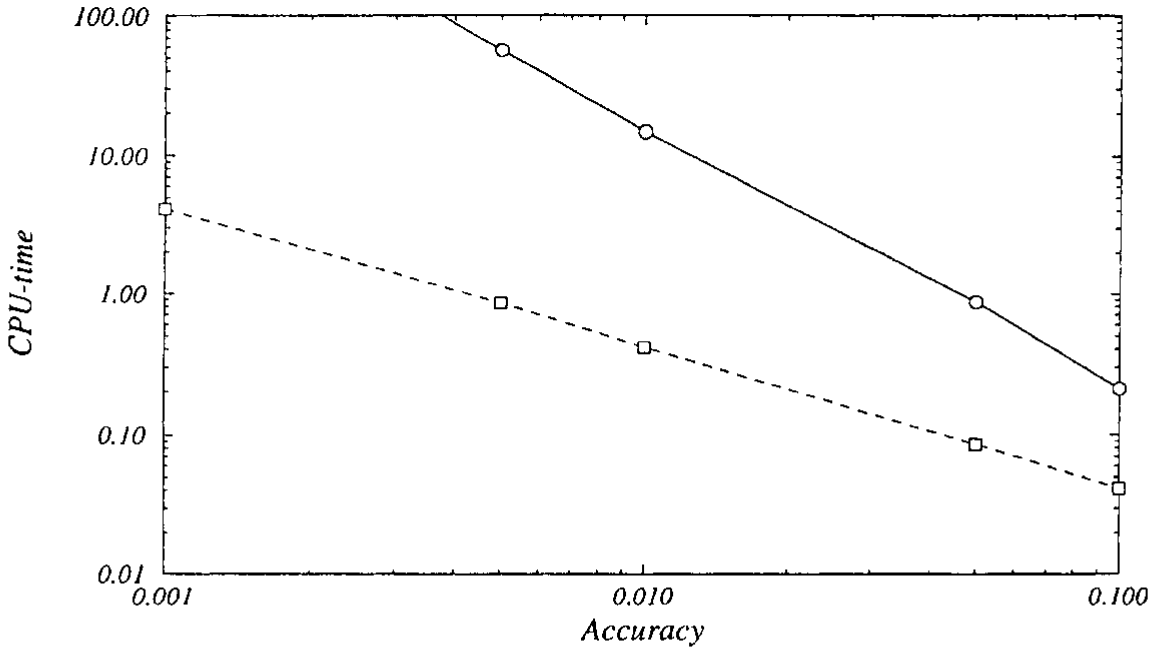
\includegraphics[width=.633\paperwidth]{images/fig-7-3-1.png}
  \caption{RT(1)(实线)和 BDM(2)(虚线)混合有限元的 CPU 用时与精度的关系}\label{fig:7.3.1}
\end{figure}

\clearpage
\section{更一般的约束问题的逼近}\label{sec:7.4}
\SourcePage{257}

本节介绍由\BookCite{babuska1971}{Babuška(1971)}和\BookCite{brezzi1974}{Brezzi(1974)}建立的抽象理论,讨论形如\eqref{eq:7.1.15}、\eqref{eq:7.1.16}的问题及其内逼近\eqref{eq:7.2.1}的解的存在性和唯一性.前面已经指出,若系数矩阵 \(\{a^{ij}\}\) 对称,这些问题等价于确定一个约束问题所对应的 Lagrange 泛函的唯一鞍点.以下分析无需这一对称性假设,所得结果也适用于更一般的问题.因此,这里在较广的意义上使用“约束问题”一词.

我们将沿用\BookCite{brezzi1974}{Brezzi(1974)}建立的理论.该理论推广并涵盖第~\ref{sec:7.2}~节只针对二阶椭圆方程\eqref{eq:7.1.1}给出的理论.事实上,对以速度 \(\boldsymbol{u}\) 和压力 \(p\) 为原始变量的 Stokes 问题作 Galerkin 逼近(见第~\BookRef{ch:9}{9}~章)时,便要用到下面的抽象理论.

更一般地说,多种边值问题的混合逼近都可以纳入这一抽象理论进行数值分析.例如,双调和算子 \(\Delta^2\) 的边值问题及其在板弯曲问题中的应用,以及采用流函数表述的 Stokes 和 Navier--Stokes 问题,都属于这种情形(见第~\BookRef{sec:10.4}{10.4}~节,亦见\BookCite{brezzi-fortin1991}{Brezzi 和 Fortin(1991)}第 IV 章).线性弹性问题的混合逼近是另一个例子(见\BookCite{brezzi-fortin1991}{Brezzi 和 Fortin(1991)}第 VII 章及其中所引文献).

\subsection{抽象表述}\label{sec:7.4.1}

先给出这一分析的一般框架.令 \(X\) 和 \(M\) 为两个实 Hilbert 空间,范数分别为 \(\|\cdot\|_X\) 和 \(\|\cdot\|_M\).设 \(X'\) 和 \(M'\) 为它们的对偶空间,即分别由 \(X\) 和 \(M\) 上的连续线性泛函组成的空间.引入两个双线性形式
\begin{equation}\label{eq:7.4.1}
  a(\cdot,\cdot)\colon X\times X\to\mathbb R,\qquad
  b(\cdot,\cdot)\colon X\times M\to\mathbb R,
\end{equation}
使对每个 \(w,v\in X\) 和 \(\mu\in M\),都有
\begin{equation}\label{eq:7.4.2}
  |a(w,v)|\le\gamma\|w\|_X\|v\|_X,\qquad
  |b(w,\mu)|\le\delta\|w\|_X\|\mu\|_M.
\end{equation}
考察下列约束问题：
\SourcePage{258}
\begin{equation}\label{eq:7.4.3}
  \left\{
  \begin{aligned}
    &\text{求 }(u,\eta)\in X\times M,\ \text{使}\\
    &a(u,v)+b(v,\eta)=\langle l,v\rangle&&\forall\,v\in X,\\
    &b(u,\mu)=\langle\sigma,\mu\rangle&&\forall\,\mu\in M,
  \end{aligned}
  \right.
\end{equation}
其中 \(l\in X'\)、\(\sigma\in M'\),\(\langle\cdot,\cdot\rangle\) 表示 \(X'\) 与 \(X\) 或 \(M'\) 与 \(M\) 之间的对偶配对.

将问题\eqref{eq:7.4.3}改写成算子形式会很方便.为双线性形式 \(a(\cdot,\cdot)\) 和 \(b(\cdot,\cdot)\) 分别引入算子 \(A\in\mathcal L(X;X')\) 和 \(B\in\mathcal L(X;M')\),其定义为
\begin{align}
  \langle Aw,v\rangle&=a(w,v)&&\forall\,w,v\in X,\label{eq:7.4.4}\\
  \langle Bv,\mu\rangle&=b(v,\mu)&&\forall\,v\in X,\ \mu\in M.\label{eq:7.4.5}
\end{align}
以 \(B^T\in\mathcal L(M;X')\) 表示 \(B\) 的伴随算子,即
\begin{equation}\label{eq:7.4.6}
  \langle B^T\mu,v\rangle=\langle Bv,\mu\rangle=b(v,\mu)
      \qquad\forall\,v\in X,\ \mu\in M.
\end{equation}
于是,可将\eqref{eq:7.4.3}写成求 \((u,\eta)\in X\times M\),使
\begin{equation}\label{eq:7.4.7}
  \begin{cases}
    Au+B^T\eta=l,&\text{在 }X'\text{ 中},\\
    Bu=\sigma,&\text{在 }M'\text{ 中}.
  \end{cases}
\end{equation}

现在定义仿射流形
\[
  X^\sigma:=\{v\in X\mid b(v,\mu)=\langle\sigma,\mu\rangle
      \quad\forall\,\mu\in M\}.
\]
显然,\(X^0=\ker B\) 是 \(X\) 的闭子空间.可以将问题\eqref{eq:7.4.3}与下列问题联系起来：
\begin{equation}\label{eq:7.4.8}
  \text{求 }u\in X^\sigma,\quad\text{使}\quad
    a(u,v)=\langle l,v\rangle\qquad\forall\,v\in X^0.
\end{equation}
容易看出,若 \((u,\eta)\) 是\eqref{eq:7.4.3}的解,则 \(u\) 是\eqref{eq:7.4.8}的解.下面将引入适当条件,使反过来也成立,并保证\eqref{eq:7.4.8}有唯一解,从而构造\eqref{eq:7.4.3}的解.

在此之前,需要证明一个关于双线性形式 \(b(\cdot,\cdot)\) 和算子 \(B\) 的等价性结论.记 \(X_\#^0\) 为 \(X^0\) 的极集,即
\begin{equation}\label{eq:7.4.9}
  X_\#^0:=\{g\in X'\mid\langle g,v\rangle=0\quad\forall\,v\in X^0\}.
\end{equation}
由于 \(X^0=\ker B\),也可写成 \(X_\#^0=(\ker B)_\#\).将 \(X\) 作如下分解：
\[
  X=X^0\oplus(X^0)^\perp.
\]
一般来说,\(\ker B=X^0\ne\{0\}\),因此 \(B\) 并非从 \(X\) 到 \(M'\) 的同构.下面要引入的一个条件等价于\SourcePage{259}\(B\) 从 \((X^0)^\perp\) 到 \(M'\) 是同构,并且 \(B^T\) 从 \(M\) 到 \(X_\#^0\) 是同构.

\begin{proposition}[]{7.4.1}
下列陈述等价：
\begin{enumerate}[label=\alph*.]
  \item 存在常数 \(\beta^*>0\),使相容性条件
  \begin{equation}\label{eq:7.4.10}
    \forall\,\mu\in M,\ \exists\,v\in X,\ v\ne0:\quad
      b(v,\mu)\ge\beta^*\|v\|_X\|\mu\|_M
  \end{equation}
  成立.
  \item 算子 \(B^T\) 是从 \(M\) 到 \(X_\#^0\) 的同构,并且
  \begin{equation}\label{eq:7.4.11}
    \|B^T\mu\|_{X'}:=\sup_{\substack{v\in X\\v\ne0}}
       \frac{\langle B^T\mu,v\rangle}{\|v\|_X}
         \ge\beta^*\|\mu\|_M\qquad\forall\,\mu\in M.
  \end{equation}
  \item 算子 \(B\) 是从 \((X^0)^\perp\) 到 \(M'\) 的同构,并且
  \begin{equation}\label{eq:7.4.12}
    \|Bv\|_{M'}:=\sup_{\substack{\mu\in M\\\mu\ne0}}
       \frac{\langle Bv,\mu\rangle}{\|\mu\|_M}
       \ge\beta^*\|v\|_X\qquad\forall\,v\in(X^0)^\perp.
  \end{equation}
\end{enumerate}
\end{proposition}

\begin{proof}
先证明 a. 与 b. 等价.由 \(B^T\) 的定义(见\eqref{eq:7.4.6})可知,\eqref{eq:7.4.10}和\eqref{eq:7.4.11}等价.因此,只需证明 \(B^T\) 是从 \(M\) 到 \(X_\#^0\) 的同构.显然,\eqref{eq:7.4.11}表明 \(B^T\) 从 \(M\) 到其值域 \(\mathcal R(B^T)\) 为单射,且逆算子连续.由此,\(\mathcal R(B^T)\) 是 \(X'\) 的闭子空间.只需证明 \(\mathcal R(B^T)=X_\#^0\).应用闭值域定理(例如,见\BookCite{yosida1974}{Yosida(1974)}第 205 页)立即得到
\[
  \mathcal R(B^T)=(\ker B)_\#=X_\#^0.
\]

接下来证明 b. 与 c. 等价.首先说明,\(X_\#^0\) 可与 \((X^0)^\perp\) 的对偶空间等同.事实上,对每个 \(g\in((X^0)^\perp)'\),可对应一个 \(\widehat g\in X'\),满足
\[
  \langle\widehat g,v\rangle=\langle g,P^\perp v\rangle\qquad\forall\,v\in X,
\]
其中 \(P^\perp\) 是到 \((X^0)^\perp\) 的正交投影.显然 \(\widehat g\in X_\#^0\),而且可以验证,\(g\mapsto\widehat g\) 是从 \(((X^0)^\perp)'\) 到 \(X_\#^0\) 的等距双射.因此,\(B^T\) 从 \(M\) 到 \(((X^0)^\perp)'\) 是同构且满足
\[
  \|(B^T)^{-1}\|_{\mathcal L(X_\#^0;M)}\le\frac1{\beta^*}
\]
的充要条件是,\(B\) 从 \((X^0)^\perp\) 到 \(M'\) 是同构且满足
\[
  \|B^{-1}\|_{\mathcal L(M';(X^0)^\perp)}\le\frac1{\beta^*}.
\]
证明完毕.\hfill\(\square\)
\end{proof}

\SourcePage{260}现在可以证明本节的主要定理.

\begin{theorem}[]{7.4.1}
假设双线性形式 \(a(\cdot,\cdot)\) 满足\eqref{eq:7.4.2},并在 \(X^0\) 上具有强制性,即存在常数 \(\alpha>0\),使
\begin{equation}\label{eq:7.4.13}
  a(v,v)\ge\alpha\|v\|_X^2\qquad\forall\,v\in X^0.
\end{equation}
还假设双线性形式 \(b(\cdot,\cdot)\) 满足\eqref{eq:7.4.2},且相容性条件\eqref{eq:7.4.10}成立.则对每个 \(l\in X'\)、\(\sigma\in M'\),\eqref{eq:7.4.8}有唯一解 \(u\),并且存在唯一的 \(\eta\in M\),使 \((u,\eta)\) 是\eqref{eq:7.4.3}的唯一解.此外,映射 \((l,\sigma)\mapsto(u,\eta)\) 是从 \(X'\times M'\) 到 \(X\times M\) 的同构,并且
\begin{align}
  \|u\|_X&\le\frac1\alpha
    \left(\|l\|_{X'}+\frac{\alpha+\gamma}{\beta^*}\|\sigma\|_{M'}\right),\label{eq:7.4.14}\\
  \|\eta\|_M&\le\frac1{\beta^*}
    \left[\left(1+\frac{\gamma}{\alpha}\right)\|l\|_{X'}
       +\frac{\gamma(\alpha+\gamma)}{\alpha\beta^*}\|\sigma\|_{M'}\right].\label{eq:7.4.15}
\end{align}
\end{theorem}

\begin{proof}
问题\eqref{eq:7.4.8}解的唯一性直接由强制性假设\eqref{eq:7.4.13}得到.

现在证明存在性.由于满足条件\eqref{eq:7.4.10},由命题~\ref{pro:7.4.1}的 c.,存在唯一的 \(u^0\in(X^0)^\perp\),使 \(Bu^0=\sigma\),且
\begin{equation}\label{eq:7.4.16}
  \|u^0\|_X\le\frac1{\beta^*}\|\sigma\|_{M'}.
\end{equation}
因此,可将\eqref{eq:7.4.8}改写为
\begin{equation}\label{eq:7.4.17}
  \text{求 }\widetilde u\in X^0,\quad\text{使}\quad
    a(\widetilde u,v)=\langle l,v\rangle-a(u^0,v)\qquad\forall\,v\in X^0,
\end{equation}
并令 \(u=\widetilde u+u^0\) 为\eqref{eq:7.4.8}的解.由 Lax--Milgram 引理(见定理~\ref{thm:5.1.1}),\eqref{eq:7.4.17}有唯一解,并且
\begin{equation}\label{eq:7.4.18}
  \|\widetilde u\|_X\le\frac1\alpha(\|l\|_{X'}+\gamma\|u^0\|_X).
\end{equation}

现在考察问题\eqref{eq:7.4.3}.由于\eqref{eq:7.4.17}可写成
\[
  \langle Au-l,v\rangle=0\qquad\forall\,v\in X^0,
\]
可知 \(Au-l\in X_\#^0\).再由命题~\ref{pro:7.4.1}的 b.,可以找到唯一的 \(\eta\in M\),使 \(Au-l=-B^T\eta\),即 \((u,\eta)\) 是\eqref{eq:7.4.3}的解,并满足
\begin{equation}\label{eq:7.4.19}
  \|\eta\|_M\le\frac1{\beta^*}\|Au-l\|_{X'}.
\end{equation}
\SourcePage{261}前面已指出,\eqref{eq:7.4.3}的每个解 \((u,\eta)\) 都给出\eqref{eq:7.4.8}的解 \(u\),所以问题\eqref{eq:7.4.3}的解也唯一.最后,合用不等式\eqref{eq:7.4.16}、\eqref{eq:7.4.18}和\eqref{eq:7.4.19},即得所需结论.\hfill\(\square\)
\end{proof}

现在可以考察抽象约束问题\eqref{eq:7.4.3}的逼近.设 \(X_h\) 和 \(M_h\) 分别为 \(X\) 和 \(M\) 的有限维子空间.给定 \(l\in X'\)、\(\sigma\in M'\),考虑求解下列问题：
\begin{equation}\label{eq:7.4.20}
  \left\{
  \begin{aligned}
    &\text{求 }(u_h,\eta_h)\in X_h\times M_h,\ \text{使}\\
    &a(u_h,v_h)+b(v_h,\eta_h)=\langle l,v_h\rangle&&\forall\,v_h\in X_h,\\
    &b(u_h,\mu_h)=\langle\sigma,\mu_h\rangle&&\forall\,\mu_h\in M_h.
  \end{aligned}
  \right.
\end{equation}
仿照无限维情形,定义空间
\[
  X_h^\sigma:=\{v_h\in X_h\mid b(v_h,\mu_h)=\langle\sigma,\mu_h\rangle
     \quad\forall\,\mu_h\in M_h\}.
\]
由于 \(M_h\) 一般是 \(M\) 的真子空间,\(X_h^\sigma\) 未必包含于 \(X^\sigma\).

与\eqref{eq:7.4.8}对应的有限维问题为
\begin{equation}\label{eq:7.4.21}
  \text{求 }u_h\in X_h^\sigma,\quad\text{使}\quad
    a(u_h,v_h)=\langle l,v_h\rangle\qquad\forall\,v_h\in X_h^0.
\end{equation}
显然,\eqref{eq:7.4.20}的每个解 \((u_h,\eta_h)\) 都给出\eqref{eq:7.4.21}的解 \(u_h\).下面将给出适当的条件,保证反过来也成立,并据此进行稳定性与收敛性分析.

\subsection{稳定性与收敛性分析}\label{sec:7.4.2}

先给出定理~\ref{thm:7.4.1}在有限维情形下的对应结果.它同时表明近似解 \((u_h,\eta_h)\) 的稳定性.

\begin{theorem}[稳定性]{7.4.2}
假定双线性形式 \(a(\cdot,\cdot)\) 满足\eqref{eq:7.4.2},并在 \(X_h^0\) 上具有强制性,即存在常数 \(\alpha_h>0\),使
\begin{equation}\label{eq:7.4.22}
  a(v_h,v_h)\ge\alpha_h\|v_h\|_X^2\qquad\forall\,v_h\in X_h^0.
\end{equation}
还假定双线性形式 \(b(\cdot,\cdot)\) 满足\eqref{eq:7.4.2}以及下列相容性条件：存在 \(\beta_h>0\),使
\begin{equation}\label{eq:7.4.23}
  \forall\,\mu_h\in M_h,\ \exists\,v_h\in X_h,\ v_h\ne0:\quad
     b(v_h,\mu_h)\ge\beta_h\|v_h\|_X\|\mu_h\|_M.
\end{equation}
则对每个 \(l\in X'\)、\(\sigma\in M'\),\eqref{eq:7.4.20}存在唯一解 \((u_h,\eta_h)\),且满足\eqref{eq:7.4.14}和\eqref{eq:7.4.15}中分别以 \(\alpha_h\) 和 \(\beta_h\) 代替 \(\alpha\) 和 \(\beta^*\) 所得的估计.若\eqref{eq:7.4.22}中的 \(\alpha_h\) 和\eqref{eq:7.4.23}中的 \(\beta_h\) 均与 \(h\) 无关,这便给出了 \((u_h,\eta_h)\) 的稳定性.
\end{theorem}

\SourcePage{262}
\begin{proof}
在定理~\ref{thm:7.4.1}中以 \(X_h\)、\(M_h\) 代替 \(X\)、\(M\),并注意到
\[
  \|l\|_{X_h'}\le\|l\|_{X'},\qquad \|\sigma\|_{M_h'}\le\|\sigma\|_{M'},
\]
即可得到上述结论.
\end{proof}
不过,必须注意,\(X_h^0\) 未必包含于 \(X^0\),因而\eqref{eq:7.4.13}并不蕴含\eqref{eq:7.4.22}.同样,由于 \(X_h\) 一般是 \(X\) 的真子空间,\eqref{eq:7.4.10}也不蕴含\eqref{eq:7.4.23}.

如第~\ref{sec:7.2.1}~节已指出的,相容性条件\eqref{eq:7.4.23}也称为 \emph{inf--sup 条件}或 \emph{Ladyzhenskaya--Babuška--Brezzi 条件}.

现在来看收敛性定理.它的证明与定理~\ref{thm:7.2.2}的证明很相似,这里仍将给出.

\begin{theorem}[收敛性]{7.4.3}
设定理~\ref{thm:7.4.1}和定理~\ref{thm:7.4.2}的假设均满足.则\eqref{eq:7.4.3}的解 \((u,\eta)\) 和\eqref{eq:7.4.20}的解 \((u_h,\eta_h)\) 满足下列误差估计：
\begin{align}
  \|u-u_h\|_X&\le\left(1+\frac{\gamma}{\alpha_h}\right)
      \inf_{v_h^*\in X_h^\sigma}\|u-v_h^*\|_X
      +\frac{\delta}{\alpha_h}\inf_{\mu_h\in M_h}\|\eta-\mu_h\|_M,\label{eq:7.4.24}\\
  \begin{split}
  \|\eta-\eta_h\|_M&\le\frac{\gamma}{\beta_h}\left(1+\frac{\gamma}{\alpha_h}\right)
      \inf_{v_h^*\in X_h^\sigma}\|u-v_h^*\|_X\\
      &\quad+\left(1+\frac{\delta}{\beta_h}+\frac{\gamma\delta}{\alpha_h\beta_h}\right)
      \inf_{\mu_h\in M_h}\|\eta-\mu_h\|_M.
  \end{split}\label{eq:7.4.25}
\end{align}
此外,还有估计
\begin{equation}\label{eq:7.4.26}
  \inf_{v_h^*\in X_h^\sigma}\|u-v_h^*\|_X
    \le\left(1+\frac{\delta}{\beta_h}\right)\inf_{v_h\in X_h}\|u-v_h\|_X.
\end{equation}
由\eqref{eq:7.4.24}至\eqref{eq:7.4.26}可知,只要\eqref{eq:7.4.22}和\eqref{eq:7.4.23}可用与 \(h\) 无关的常数成立,收敛就是最优的.
\end{theorem}

\begin{proof}
取 \(v_h\in X_h\)、\(v_h^*\in X_h^\sigma\) 和 \(\mu_h\in M_h\).将\eqref{eq:7.4.3}和\eqref{eq:7.4.20}的第一个方程相减,可得
\[
  a(u_h-v_h^*,v_h)+b(v_h,\eta_h-\mu_h)
     =a(u-v_h^*,v_h)+b(v_h,\eta-\mu_h).
\]
取 \(v_h=u_h-v_h^*\in X_h^0\),由\eqref{eq:7.4.22}和\eqref{eq:7.4.2}可得
\[
  \|u_h-v_h^*\|_X
     \le\frac1{\alpha_h}\bigl(\gamma\|u-v_h^*\|_X+\delta\|\eta-\mu_h\|_M\bigr),
\]
所以\eqref{eq:7.4.24}成立.

为得到\eqref{eq:7.4.25},从相容性条件\eqref{eq:7.4.23}出发.对每个 \(\mu_h\in M_h\),有
\SourcePage{263}
\[
  \|\eta_h-\mu_h\|_M
    \le\frac1{\beta_h}\sup_{\substack{v_h\in X_h\\v_h\ne0}}
       \frac{b(v_h,\eta_h-\mu_h)}{\|v_h\|_X}.
\]
另一方面,由\eqref{eq:7.4.3}和\eqref{eq:7.4.20}的第一个方程相减可知
\[
  b(v_h,\eta_h-\mu_h)=a(u-u_h,v_h)+b(v_h,\eta-\mu_h).
\]
由\eqref{eq:7.4.2}得到
\[
  \|\eta_h-\mu_h\|_M
    \le\frac1{\beta_h}\bigl(\gamma\|u-u_h\|_X+\delta\|\eta-\mu_h\|_M\bigr).
\]
结合\eqref{eq:7.4.24},即可得到\eqref{eq:7.4.25}.

最后,证明\eqref{eq:7.4.26}.对于每个 \(v_h\in X_h\),由\eqref{eq:7.4.23}和命题~\ref{pro:7.4.1}可知,存在唯一的 \(z_h\in X_h\cap(X_h^0)^\perp\),使
\[
  b(z_h,\mu_h)=b(u-v_h,\mu_h)\qquad\forall\,\mu_h\in M_h,
\]
并且
\[
  \|z_h\|_X\le\frac{\delta}{\beta_h}\|u-v_h\|_X.
\]
令 \(v_h^*:=z_h+v_h\).由于对每个 \(\mu_h\in M_h\) 都有 \(b(u,\mu_h)=\langle\sigma,\mu_h\rangle\),显然 \(v_h^*\in X_h^\sigma\).此外,
\[
  \|u-v_h^*\|_X\le\|u-v_h\|_X+\|z_h\|_X
    \le\left(1+\frac{\delta}{\beta_h}\right)\|u-v_h\|_X.
\]
于是\eqref{eq:7.4.26}成立.\hfill\(\square\)
\end{proof}

\begin{note}\NumberedNote{note:7.4.1}
考察定理~\ref{thm:7.2.2}的证明,特别是\eqref{eq:7.2.17},可看出,在 \(X_h^0\subset X^0\) 的条件下,只用 \(\inf_{v_h\in X_h}\|u-v_h\|_X\) 即可估计 \(\|u-u_h\|_X\).此外,即使相容性条件\eqref{eq:7.4.10}和\eqref{eq:7.4.23}不成立,误差估计\eqref{eq:7.4.24}仍然成立.\hfill\(\square\)
\end{note}

\begin{note}\NumberedNote{note:7.4.2}{\heiti(伪模态)}
相容性条件\eqref{eq:7.4.23}是保证 \(\eta_h\) 唯一的必要条件.事实上,它可以写成：若 \(\mu_h\in M_h\),并且对每个 \(v_h\in X_h\) 都有 \(b(v_h,\mu_h)=0\),则 \(\mu_h=0\).

所以,若\eqref{eq:7.4.23}不成立,则存在非零的 \(\mu_h^*\in M_h\),使
\[
  b(v_h,\mu_h^*)=0\qquad\forall\,v_h\in X_h.
\]
因此,若 \((u_h,\eta_h)\) 是\eqref{eq:7.4.20}的解,则对每个 \(\tau\in\mathbb R\),\((u_h,\eta_h+\tau\mu_h^*)\) 也是同一个问题的解.

任何这样的 \(\mu_h^*\) 都称为{\heiti 伪模态}(或{\heiti 寄生模态}),因为数值问题\eqref{eq:7.4.20}无法检测到它.因而它可能使方法不稳定(另见第~\BookRef{sec:9.2.2}{9.2.2}~节).\hfill\(\square\)
\end{note}

\subsection{如何验证一致相容性条件}\label{sec:7.4.3}
\SourcePage{264}

在大多数应用中,验证\eqref{eq:7.4.22}关于 \(h\) 一致成立并不困难,例如见第~\ref{sec:7.2.1}~节和第~\BookRef{ch:9}{9}~章.较困难的是证明相容性条件\eqref{eq:7.4.23}关于 \(h\) 一致成立.

\BookCite{fortin1977}{Fortin(1977)}提出了这方面的第一个判据(见引理~\ref{lem:7.2.1}).这里给出一般的抽象表述,其证明思路与前面相同.

\begin{lemma}[Fortin]{7.4.1}
假设相容性条件\eqref{eq:7.4.10}成立,并且存在算子 \(\tau_h\colon X\to X_h\),使
\[
  \begin{aligned}
    \text{(i)}\quad &b(v-\tau_h(v),\mu_h)=0 &&\forall\,v\in X,\ \mu_h\in M_h,\\
    \text{(ii)}\quad &\|\tau_h(v)\|_X\le C_*\|v\|_X &&\forall\,v\in X,
  \end{aligned}
\]
其中 \(C_*>0\) 与 \(h\) 无关.则相容性条件\eqref{eq:7.4.23}成立,且可取 \(\beta=\beta^*/C_*\).
\end{lemma}

另一种值得考察的情形是取 \(X=(H_0^1(\Omega))^d\)、\(M=L_0^2(\Omega)\),并令 \(a(\boldsymbol{w},\boldsymbol{v})=\nu(\nabla\boldsymbol{w},\nabla\boldsymbol{v})\)、\(b(\boldsymbol{v},q)=-(q,\operatorname{div}\boldsymbol{v})\),其中 \(\nu>0\).这些是 Stokes 问题变分形式中的函数空间和双线性形式(见第~\BookRef{ch:9}{9}~章).在这种情形下,\BookCite{verfurth1984b}{Verfürth(1984b)}证明了下列结果.

\begin{lemma}[Verfürth]{7.4.2}
设 \(\mathcal T_h\) 是 \(\overline\Omega\) 的一族拟一致剖分.假设 \(M_h\subset H^1(\Omega)\cap L_0^2(\Omega)\),且存在 \(\widehat\beta>0\),使
\begin{equation}\label{eq:7.4.27}
  \forall\,q_h\in M_h,\ \exists\,\boldsymbol{v}_h\in X_h,\ \boldsymbol{v}_h\ne0:\quad
     b(\boldsymbol{v}_h,q_h)\ge\widehat\beta\|\boldsymbol{v}_h\|_0\|q_h\|_1.
\end{equation}
再假设存在算子 \(R_h\colon X\to X_h\) 和常数 \(K>0\),使
\begin{equation}\label{eq:7.4.28}
  \|\boldsymbol{v}-R_h(\boldsymbol{v})\|_0+h\|\boldsymbol{v}-R_h(\boldsymbol{v})\|_1
     \le Kh|\boldsymbol{v}|_1\qquad\forall\,\boldsymbol{v}\in X.
\end{equation}
则相容性条件\eqref{eq:7.4.23}关于 \(h\) 一致成立.
\end{lemma}

\begin{proof}
首先,由逆不等式\eqref{eq:6.3.21}可知,对每个 \(\boldsymbol{v}_h\in X_h\),都有
\[
  \|\boldsymbol{v}_h\|_1\le Ch^{-1}\|\boldsymbol{v}_h\|_0.
\]
因此,条件\eqref{eq:7.4.27}蕴含
\begin{equation}\label{eq:7.4.29}
  \forall\,q_h\in M_h,\ \exists\,\boldsymbol{v}_h\in X_h,\ \boldsymbol{v}_h\ne0:\quad
     b(\boldsymbol{v}_h,q_h)\ge K_1h\|\boldsymbol{v}_h\|_1\|q_h\|_1.
\end{equation}
回顾一下,对每个 \(q_h\in M_h\),都存在 \(\boldsymbol{w}\in X\),使 \(\operatorname{div}\boldsymbol{w}=-q_h\),并且
\begin{equation}\label{eq:7.4.30}
  \|\boldsymbol{w}\|_1\le K_2\|q_h\|_0
\end{equation}
\SourcePage{265}(例如,见\BookCite{girault-raviart1986}{Girault 和 Raviart(1986)}第 24 页).于是,由\eqref{eq:7.4.28}得到
\begin{equation}\label{eq:7.4.31}
  \begin{aligned}
    \|R_h(\boldsymbol{w})\|_1
      &\le\|R_h(\boldsymbol{w})-\boldsymbol{w}\|_1+\|\boldsymbol{w}\|_1\\
      &\le(1+K)\|\boldsymbol{w}\|_1\le K_2(1+K)\|q_h\|_0.
  \end{aligned}
\end{equation}
若 \(q_h\) 满足
\begin{equation}\label{eq:7.4.32}
  \|q_h\|_0\le KK_2h\|q_h\|_1,
\end{equation}
则由\eqref{eq:7.4.29}可得
\begin{equation}\label{eq:7.4.33}
  b(\boldsymbol{v}_h,q_h)\ge\frac{K_1}{KK_2}\|\boldsymbol{v}_h\|_1\|q_h\|_0.
\end{equation}
若
\begin{equation}\label{eq:7.4.34}
  \|q_h\|_0>KK_2h\|q_h\|_1,
\end{equation}
则由\eqref{eq:7.4.28}、\eqref{eq:7.4.30}和\eqref{eq:7.4.31}得到
\begin{equation}\label{eq:7.4.35}
  \begin{aligned}
    b(R_h(\boldsymbol{w}),q_h)
      &=b(\boldsymbol{w},q_h)+b(R_h(\boldsymbol{w})-\boldsymbol{w},q_h)\\
      &\ge\|q_h\|_0^2-\|R_h(\boldsymbol{w})-\boldsymbol{w}\|_0\|q_h\|_1\\
      &\ge\|q_h\|_0^2-KK_2h\|q_h\|_0\|q_h\|_1\\
      &\ge\frac{1}{K_2(1+K)}
         (\|q_h\|_0-KK_2h\|q_h\|_1)\|R_h(\boldsymbol{w})\|_1.
  \end{aligned}
\end{equation}
其中 \(b(R_h(\boldsymbol{w})-\boldsymbol{w},q_h)\) 一项用了分部积分.

结合\eqref{eq:7.4.29}和\eqref{eq:7.4.35},容易证明,对每个满足\eqref{eq:7.4.34}的 \(q_h\in M_h\),都存在 \(\boldsymbol{z}_h\in X_h\)、\(\boldsymbol{z}_h\ne0\),使
\begin{equation}\label{eq:7.4.36}
  b(\boldsymbol{z}_h,q_h)\ge Q(h\|q_h\|_1)\|\boldsymbol{z}_h\|_1,
\end{equation}
其中
\[
  Q(\xi):=\max\left\{K_1\xi,\frac{1}{K_2(1+K)}
       (\|q_h\|_0-KK_2\xi)\right\},\qquad \xi>0.
\]
最后,求 \(Q(\xi)\) 在 \(\xi>0\) 上的最小值.由\eqref{eq:7.4.33}和\eqref{eq:7.4.36},可知\eqref{eq:7.4.23}成立,且可取
\[
  \beta=K_1K_2^{-1}[K_1(1+K)+K]^{-1}.
\]
\hfill\(\square\)
\end{proof}

注意,\eqref{eq:7.4.27}与\eqref{eq:7.4.23}不同,其右端使用的是另一组范数.已有证明表明,一些常用于逼近 Stokes 问题的有限元空间满足\eqref{eq:7.4.27}.例如,第~\BookRef{sec:9.3.2}{9.3.2}~节将介绍 Taylor--Hood 单元和 Bercovier--Pironneau 单元,其证明分别见\BookCite{fortin1993}{Fortin(1993)}和\BookCite{bercovier-pironneau1979}{Bercovier 和 Pironneau(1979)}.

此外,在适当假设下,多种 \(X_h\) 都满足逼近性质\eqref{eq:7.4.28},例如见\eqref{eq:3.5.22}或\BookCite{clement1975}{Clément(1975)}.

\SourcePage{266}对于 Stokes 问题,还有一些可用来验证一致相容性条件\eqref{eq:7.4.23}的判据,由\BookCite{boland-nicolaides1983}{Boland 和 Nicolaides(1983)}及\BookCite{stenberg1984}{Stenberg(1984)}提出(另见\BookCite{gunzburger1989}{Gunzburger(1989)}第 16–21 页和\BookCite{girault-raviart1986}{Girault 和 Raviart(1986)}第 129–132 页).这些判据的基本做法是将 \(\Omega\) 划分成若干宏单元,只在各个宏单元上局部验证相容性条件\eqref{eq:7.4.23}.

\section{补充说明}\label{sec:7.5}

对于混合方法,已有关于 \(u-u_h\) 在 \(L^\infty(\Omega)\) 范数下的误差估计,例如见\BookCite{scholz1977}{Scholz(1977)}、\BookCite{douglas-roberts1985}{Douglas 和 Roberts(1985)}及\BookCite{gastaldi-nochetto1987}{Gastaldi 和 Nochetto(1987)}.

把本章的结果推广到一般的椭圆型算子
\[
  Lw:=-\sum_{i,j=1}^d D_i(a_{ij}D_jw)+\sum_{i=1}^d c_iD_iw+a_0w
\]
时可能遇到一些困难.对偶混合表述的情形见\BookCite{douglas-roberts1985}{Douglas 和 Roberts(1985)}的分析.

另一种推广涉及可写成如下形式的问题：
\[
  \left\{
  \begin{aligned}
    &\text{求 }(u,\eta)\in X\times M,\ \text{使}\\
    &a(u,v)+b(v,\eta)=\langle l,v\rangle&&\forall\,v\in X,\\
    &b(u,\mu)-d(\eta,\mu)=\langle\sigma,\mu\rangle&&\forall\,\mu\in M,
  \end{aligned}
  \right.
\]
其中 \(d(\cdot,\cdot)\) 是 \(M\times M\) 上连续且非负的双线性形式.关于该问题的分析,见\BookCite{roberts-thomas1991}{Roberts 和 Thomas(1991)},另见第~\BookRef{sec:9.6.7}{9.6.7}~节.

Brezzi 理论的另一项推广涉及下列问题：
\[
  \left\{
  \begin{aligned}
    &\text{求 }(u,\eta)\in X\times M,\ \text{使}\\
    &a(u,v)+b_1(v,\eta)=\langle l,v\rangle&&\forall\,v\in X,\\
    &b_2(u,\mu)=\langle\sigma,\mu\rangle&&\forall\,\mu\in M,
  \end{aligned}
  \right.
\]
其中双线性形式 \(b_1\) 和 \(b_2\) 彼此不同.见\BookCite{nicolaides1982}{Nicolaides(1982)}及\BookCite{bernardi-canuto-maday1988}{Bernardi、Canuto 和 Maday(1988)},后一项工作以 Stokes 问题的 Chebyshev 逼近为出发点.

\chapter{定常对流--扩散问题}\label{ch:8}
\SourcePage{267}

本章考察对流项远强于扩散项的二阶线性椭圆方程.

首先通过一个简单的一维有限差分格式,说明采用 Galerkin 法时遇到的困难.第一种补救措施是采用“迎风”格式,引入“数值黏性”,使计算算法稳定下来.不过,这种处理只有一阶精度.

随后在二维和三维情形下,分别对有限元逼近和谱配置逼近介绍并分析更一般、具有高阶精度的稳定化方法.另有一节给出采用这些方法得到的一些数值结果.

最后,简要说明一种基于区域分解技术的异质方法.

对流占优问题的最优稳定化方法仍是一个活跃的研究领域.有兴趣的读者可继续关注最新文献.

\section{数学表述}\label{sec:8.1}

现在考察第~\ref{sec:6.1}~节引入的二阶线性椭圆算子
\begin{equation}\label{eq:8.1.1}
  Lz:=-\sum_{i,j=1}^d D_i(a_{ij}D_jz)+\sum_{i=1}^d D_i(b_iz)+a_0z
\end{equation}
及其对应的双线性形式
\begin{equation}\label{eq:8.1.2}
  a(z,v):=\int_\Omega\left[\sum_{i,j=1}^d a_{ij}D_jzD_iv-\sum_{i=1}^d b_izD_iv+a_0zv\right].
\end{equation}
假设 \(V\) 是 \(H^1(\Omega)\) 的一个闭子空间,且 \(a(\cdot,\cdot)\) 在 \(V\times V\) 上连续并具有强制性.也就是说,存在常数 \(\gamma>0\) 和 \(\alpha>0\),使
\SourcePage{268}
\begin{align}
  |a(z,v)|&\le\gamma\|z\|_1\|v\|_1&&\forall\,z,v\in V,\label{eq:8.1.3}\\
  a(v,v)&\ge\alpha\|v\|_1^2&&\forall\,v\in V.\label{eq:8.1.4}
\end{align}
如第~\ref{sec:6.1.2}~节所述,对系数 \(a_{ij}\)、\(b_i\) 和 \(a_0\) 作适当假设,就可保证\eqref{eq:8.1.3}和\eqref{eq:8.1.4}成立.例如,若 \(V=H_0^1(\Omega)\),且\eqref{eq:6.1.19}在 \(\eta=0\) 时成立,则可以选取
\begin{equation}\label{eq:8.1.5}
  \alpha=\frac{\alpha_0}{1+C_\Omega},
\end{equation}
其中 \(\alpha_0\) 和 \(C_\Omega\) 分别为椭圆性常数和 Poincaré 常数(见定义~\ref{def:6.1.1}和\eqref{eq:1.3.2}).此外,\(\gamma\) 可表示为
\begin{equation}\label{eq:8.1.6}
  \gamma=C_{d,\Omega}\left(
    \max_{1\le i,j\le d}\|a_{ij}\|_{L^\infty(\Omega)}
      +\|\boldsymbol{b}\|_{L^\infty(\Omega)}+\|a_0\|_{L^\infty(\Omega)}\right),
\end{equation}
其中 \(C_{d,\Omega}\) 是一个依赖于空间维数 \(d\) 和区域 \(\Omega\) 的适当常数.

回顾一下,在上述假设\eqref{eq:8.1.3}和\eqref{eq:8.1.4}下,Lax--Milgram 引理(见定理~\ref{thm:5.1.1})保证存在唯一的解
\begin{equation}\label{eq:8.1.7}
  u\in V:\quad a(u,v)=\mathcal F(v)\qquad\forall\,v\in V,
\end{equation}
其中 \(\mathcal F(\cdot)\) 是 Hilbert 空间 \(V\) 上的连续线性泛函.

第~\ref{sec:6.2.1}~节已经介绍了用 Galerkin 法逼近\eqref{eq:8.1.7}的解 \(u\).不过,第~\ref{sec:6.1.4}~节也指出,若强制性常数 \(\alpha\) 与连续性常数 \(\gamma\) 相比很小,Galerkin 法的表现可能不佳.特别是,若椭圆性常数 \(\alpha_0\) 与 \(\|\boldsymbol{b}\|_{L^\infty(\Omega)}\) 或 \(\|a_0\|_{L^\infty(\Omega)}\) 相比很小,误差估计\eqref{eq:6.2.8}中的乘法常数 \(C\) 就可能很大.

下面各节旨在说明,这类困难在采用 Galerkin 法时确实可能出现,随后将介绍几种克服这些困难的方法.

第~\BookRef{sec:8.2}{8.2}~节先从一个简单的一维例子出发,说明不稳定性的来源.接着,第~\BookRef{sec:8.3}{8.3}~节介绍一些最常见的补救措施,重点讨论有限元逼近和谱逼近.

\section{一个一维例题}\label{sec:8.2}

\begin{example}[一维对流--扩散方程]\label{ex:8.2-model}
考虑一维对流--扩散方程
\SourcePage{269}
\begin{equation}\label{eq:8.2.1}
  \begin{cases}
    -\varepsilon D^2u+bDu=0,\quad 0<x<1,\\
    u(0)=0,\\
    u(1)=1,
  \end{cases}
\end{equation}
其中 \(\varepsilon>0\)、\(b>0\).其精确解为
\[
  u(x)=(e^{b/\varepsilon}-1)^{-1}(e^{bx/\varepsilon}-1).
\]
若 \(\varepsilon/b\) 充分小,则解在 \(x=1\) 附近有一个宽度为 \(O(\varepsilon/b)\) 的边界层.
\end{example}

\subsection{Galerkin 逼近与中心有限差分}\label{sec:8.2.1}

首先,在均匀网格上用分片线性有限元 Galerkin 法逼近\eqref{eq:8.2.1}\@.为此,选定正整数 \(M\),令 \(h:=1/M\),\(x_j:=jh\),\(j=0,\ldots,M\).然后,按照笔记~\ref{note:6.2.2}后半部分的做法逼近非齐次 Dirichlet 问题\eqref{eq:8.2.1},取 \(V_h=X_h^1\cap H_0^1(0,1)\) 和 \(V_h^*=\{v_h\in X_h^1\mid v_h(0)=0,\ v_h(1)=1\}\),其中 \(X_h^1\) 按\eqref{eq:3.2.4}定义.

由此得到线性方程组
\begin{equation}\label{eq:8.2.2}
  A\boldsymbol{\xi}=\boldsymbol{F},
\end{equation}
其中
\begin{align}
  A&:=\operatorname{tridiag}\left(-\frac{\varepsilon}h-\frac b2,\
     \frac{2\varepsilon}h,-\frac{\varepsilon}h+\frac b2\right),\label{eq:8.2.3}\\
  \boldsymbol{F}&:=\left(0,\ldots,0,\frac{\varepsilon}h-\frac b2\right),\label{eq:8.2.4}\\
  \boldsymbol{\xi}&:=\{u_h(x_j)\}_{j=1,\ldots,M-1}.\label{eq:8.2.5}
\end{align}
假设 \(2\varepsilon\ne bh\),容易看出\eqref{eq:8.2.2}的解为
\begin{equation}\label{eq:8.2.6}
  \xi_j=u_h(x_j)=
    \frac{\left(\dfrac{1+\mathrm{Pe}}{1-\mathrm{Pe}}\right)^j-1}
         {\left(\dfrac{1+\mathrm{Pe}}{1-\mathrm{Pe}}\right)^M-1},
   \qquad j=1,\ldots,M-1,
\end{equation}
其中
\begin{equation}\label{eq:8.2.7}
  \mathrm{Pe}:=\frac{bh}{2\varepsilon}
\end{equation}
是 \emph{Péclet 数}.若 \(\mathrm{Pe}>1\),则 \((1+\mathrm{Pe})/(1-\mathrm{Pe})<0\),所以解 \(u_h\) 出现振荡.显然,给定 \(\varepsilon\) 和 \(b\),原则上总可以把网格尺寸 \(h\) 取得足够小,使 \(\mathrm{Pe}\le1\),从而避免振荡(见\figref{fig:8.2.1}).然而,\SourcePage{270}当 \(\varepsilon\) 相对于 \(b\) 很小时,这种做法通常不切实际,因为所得线性方程组的未知量太多,在更高维情形下甚至可能无法求解.

\begin{figure}[!htbp]
  \centering
  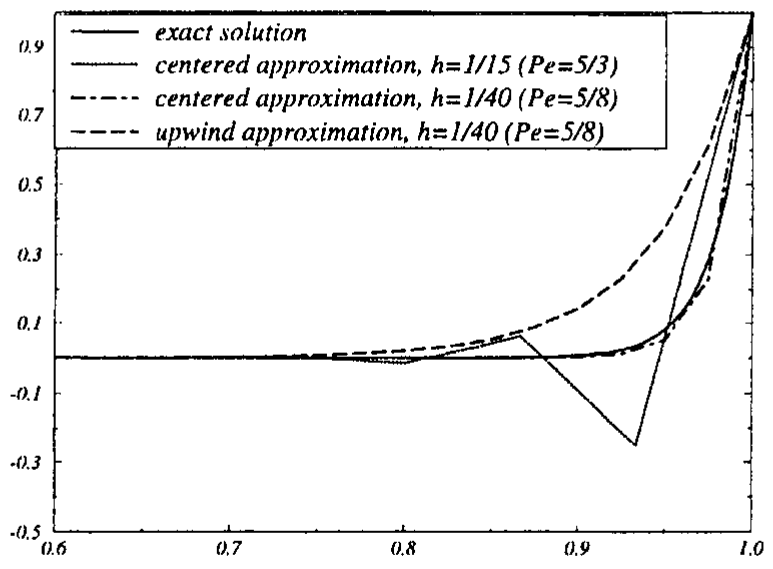
\includegraphics[width=.421\paperwidth]{images/fig-8-2-1.png}
  \caption{\(\varepsilon=1/50\)、\(b=1\) 时\eqref{eq:8.2.1}的精确解、中心差分逼近和迎风差分逼近}\label{fig:8.2.1}
\end{figure}

因此可以先得出如下结论：若对流--扩散问题存在边界层,且网格尺寸 \(h\) 大于 \(2\varepsilon/b\),Galerkin 解就可能出现振荡.第~\BookRef{sec:8.3}{8.3}~节将介绍如何克服这一困难.

线性方程组\eqref{eq:8.2.2}与用\emph{中心有限差分}逼近\eqref{eq:8.2.1}所得的方程组等价.这里之所以一致,是因为采用了均匀网格,且对流速度 \(b\) 为常数.事实上,中心差分格式为
\begin{equation}\label{eq:8.2.8}
  \begin{cases}
    -\varepsilon\dfrac{u_{j+1}-2u_j+u_{j-1}}{h^2}
        +b\dfrac{u_{j+1}-u_{j-1}}{2h}=0,\quad j=1,\ldots,M-1,\\[6pt]
    u_0=0,\\
    u_M=1,
  \end{cases}
\end{equation}
其中 \(u_j\) 是 \(u(x_j)\) 的近似值.这是一组线性差分方程,其解为 \(u_j=\xi_j\),其中 \(\xi_j\) 由\eqref{eq:8.2.6}给出(例如,见\BookCite{isaacson-keller1966}{Isaacson 和 Keller(1966)}第 8.4 节).因此,采用分片线性多项式的 Galerkin 法与中心有限差分逼近等价.

\begin{note}\NumberedNote{note:8.2.1}
暂且离开问题\eqref{eq:8.2.1},考虑反应--扩散问题
\SourcePage{271}
\[
  \begin{cases}
    -\varepsilon D^2u+a_0u=0,\quad 0<x<1,\\
    u(0)=0,\\
    u(1)=1,
  \end{cases}
\]
其中 \(\varepsilon>0\)、\(a_0>0\).其解为
\[
  u(x)=\frac{\sinh(\sqrt{a_0/\varepsilon}\,x)}{\sinh(\sqrt{a_0/\varepsilon})}.
\]
只要 \(\varepsilon/a_0\) 足够小,解就在 \(x=1\) 附近有一个宽度为 \(O(\sqrt{\varepsilon/a_0})\) 的边界层.

中心有限差分格式用下式逼近精确解 \(u(x_j)\)：
\begin{equation}\label{eq:8.2.9}
  \xi_j=(\tau_2^M-\tau_1^M)^{-1}(\tau_2^j-\tau_1^j),\qquad j=1,\ldots,M-1,
\end{equation}
其中 \(\tau_1=1+\sigma-\sqrt{\sigma(2+\sigma)}\),\(\tau_2=1+\sigma+\sqrt{\sigma(2+\sigma)}\),且 \(\sigma:=a_0h^2/(2\varepsilon)\).由于对任意网格尺寸 \(h\) 都有 \(0<\tau_1<1<\tau_2\),序列 \(\xi_j\) 单调递增.因此,无论 \(h\) 取何值,这一有限差分格式都不会产生振荡.

另一方面,采用分片线性有限元 Galerkin 法逼近该反应--扩散问题,得到下列方程组：
\[
  \varepsilon\sum_{i=0}^M\xi_i\int_0^1D\varphi_iD\varphi_j
    +a_0\sum_{i=0}^M\xi_i\int_0^1\varphi_i\varphi_j=0,\qquad j=1,\ldots,M-1,
\]
其中 \(\varphi_i\) 是包含端点的节点基函数,且 \(\xi_0=0\)、\(\xi_M=1\).算出积分后,得到代数方程组
\[
  \begin{cases}
    -\varepsilon\dfrac{\xi_{j+1}-2\xi_j+\xi_{j-1}}h
       +a_0h\dfrac{\xi_{j+1}+4\xi_j+\xi_{j-1}}6=0,\quad j=1,\ldots,M-1,\\[6pt]
    \xi_0=0,\\
    \xi_M=1.
  \end{cases}
\]
当 \(\sigma\ne3\) 时,相应的解形如\eqref{eq:8.2.9},但其中
\[
  \tau_1=\frac{3+2\sigma-\sqrt{3\sigma(\sigma+6)}}{3-\sigma},\qquad
  \tau_2=\frac{3+2\sigma+\sqrt{3\sigma(\sigma+6)}}{3-\sigma}.
\]
这两个特征根的符号都与 \(3-\sigma\) 相同.因此,当 \(\sigma>3\),即 \(h>\sqrt{6\varepsilon/a_0}\) 时,有限元解会出现振荡.

这一次,导致数值振荡的是零阶项 \(a_0u\).事实上,质量矩阵 \(M_{ij}:=\int_0^1\varphi_i\varphi_j\) 是恒等算子在有限元下的表示.若将它换成{\heiti 集中质量矩阵} \(\widehat M_{ij}:=(\sum_{k=0}^M M_{ik})\delta_{ij}\),可以立即验证,内点上的集中质量矩阵为 \(\widehat M=hI\).将内点方程除以 \(h\),就恰好得到有限差分格式,从而获得无条件稳定的解.关于时间依赖问题中的质量集中处理,见第~\BookRef{sec:11.4}{11.4}~节.\hfill\(\square\)
\end{note}

\subsection{迎风有限差分与数值扩散}\label{sec:8.2.2}
\SourcePage{272}

注意,问题\eqref{eq:8.2.1}中 \(b>0\),输运由左向右.因此,可以考虑用向后(\emph{迎风})有限差分逼近 \(bDu\).

所得格式可写为
\begin{equation}\label{eq:8.2.10}
  \begin{cases}
    -\varepsilon\dfrac{\widetilde u_{j+1}-2\widetilde u_j+\widetilde u_{j-1}}{h^2}
       +b\dfrac{\widetilde u_j-\widetilde u_{j-1}}h=0,\quad j=1,\ldots,M-1,\\[6pt]
    \widetilde u_0=0,\\
    \widetilde u_M=1,
  \end{cases}
\end{equation}
其解为
\begin{equation}\label{eq:8.2.11}
  \widetilde u_j=\frac{(1+2\mathrm{Pe})^j-1}{(1+2\mathrm{Pe})^M-1},
    \qquad j=1,\ldots,M-1.
\end{equation}
这一次,\(\widetilde u_j\) 不再振荡.事实上,对任意正的 \(\varepsilon\)、\(b\) 和 \(h\),均有 \(1+2\mathrm{Pe}>1\),所以 \(\widetilde u_j\) 随 \(j\) 递增(见\figref{fig:8.2.1}).

可以看到,这一迎风格式引入的局部截断误差为 \(O(h)\),而中心差分格式的局部截断误差为 \(O(h^2)\).需要注意,分片线性有限元的误差在 \(H^1\) 范数下按 \(O(h)\) 衰减(见\eqref{eq:6.2.8}),在最大范数下却按 \(O(h^2)\) 衰减(见\BookCite{ciarlet1968}{Ciarlet(1968)}).这与前面所见的一致：对常系数一维边值问题,均匀网格上的分片线性有限元与中心有限差分一致.

迎风格式的精度较低,但当 Péclet 数 \(\mathrm{Pe}>1\) 时,确实更适合用来逼近\eqref{eq:8.2.1}的解.

也可以从另一个角度解释这一事实.对 \(Du\) 的迎风逼近可以写成
\[
  \frac{\widetilde u_j-\widetilde u_{j-1}}h
   =\frac{\widetilde u_{j+1}-\widetilde u_{j-1}}{2h}
    -\frac h2\frac{\widetilde u_{j+1}-2\widetilde u_j+\widetilde u_{j-1}}{h^2}.
\]
因此,它相当于对正则化算子 \(D-\tfrac h2D^2\) 作中心差分逼近.换言之,迎风逼近引入了数值耗散,可将其看作对人工黏性项 \(-\tfrac h2D^2u\) 的直接离散.这通常称为\emph{数值扩散}(或\emph{数值黏性}).这也从另一个角度说明了迎风差分格式为何只有一阶精度.

迎风差分格式可以解释为\eqref{eq:8.2.1}的 Petrov--Galerkin 逼近.在这种方法中,近似解与试验函数分别取自不同的空间,通常记为 \(W_h\) 和 \(V_h\).逼近\eqref{eq:8.2.1}时,\SourcePage{273}可取 \(W_h=X_h^1\cap H_0^1(0,1)\)；相应的仿射子空间 \(W_h^*=\{v_h\in X_h^1\mid v_h(0)=0,\ v_h(1)=1\}\) 负责满足非齐次 Dirichlet 条件.为定义试验函数空间 \(V_h\),考察分片二次函数
\begin{equation}\label{eq:8.2.12}
  \sigma_2(x):=
  \begin{cases}
    -3x(1+x),&-1\le x\le0,\\
    -3x(1-x),&0\le x\le1,\\
    0,&|x|\ge1.
  \end{cases}
\end{equation}
这样便可引入有限维空间
\begin{equation}\label{eq:8.2.13}
  V_h=\operatorname{span}\{\psi_1,\ldots,\psi_{M-1}\},
\end{equation}
其中
\begin{equation}\label{eq:8.2.14}
  \psi_j(x):=\varphi_j(x)+\sigma_2(h^{-1}x-j),\qquad j=1,\ldots,M-1,
\end{equation}
而 \(\varphi_j\) 是 \(W_h\) 中与节点 \(x_j\) 对应的基函数.

容易验证(例如,见\BookCite{mitchell-griffiths1980}{Mitchell 和 Griffiths(1980)}第 221–223 页),\eqref{eq:8.2.10}对应的线性方程组与下列 Petrov--Galerkin 问题的方程组等价：
\[
  \text{求 }u_h\in W_h^*,\quad\text{使}\quad
  \int_0^1(\varepsilon Du_hDv_h+bDu_hv_h)=0\qquad\forall\,v_h\in V_h.
\]

\subsection{谱逼近}\label{sec:8.2.3}

本小节考察对流--扩散问题\eqref{eq:8.2.1}的 Chebyshev 配置逼近.可以看到,对流项占优时确实会出现振荡,但谱解仍满足某种形式的最大值原理.这些结果由\BookCite{canuto1988}{Canuto(1988)}给出.

为简便起见,在区间 \((-1,1)\) 上讨论与前面相同的 Dirichlet 问题,即
\begin{equation}\label{eq:8.2.15}
  \begin{cases}
    -\varepsilon D^2u+bDu=0,\quad -1<x<1,\\
    u(-1)=0,\\
    u(1)=1.
  \end{cases}
\end{equation}
对 \(N\ge2\),定义
\begin{equation}\label{eq:8.2.16}
  V_N^*:=\{v_N\in\mathbb P_N\mid v_N(-1)=0,\ v_N(1)=1\}
\end{equation}
及
\begin{equation}\label{eq:8.2.17}
  V_N=\mathbb P_N^0:=\{v_N\in\mathbb P_N\mid v_N(-1)=v_N(1)=0\},
\end{equation}
\SourcePage{274}则 Chebyshev 谱问题为
\begin{equation}\label{eq:8.2.18}
  \text{求 }u_N\in V_N^*,\quad\text{使}\quad
  \varepsilon\left(Du_N,\frac{D(v_Nw)}w\right)_N
       +b(Du_N,v_N)_N=0\qquad\forall\,v_N\in V_N,
\end{equation}
其中 \((\cdot,\cdot)_N\) 是\eqref{eq:4.2.4}中引入的离散内积,Chebyshev 节点和权重分别由\eqref{eq:4.3.12}和\eqref{eq:4.3.13}给出.

注意,\eqref{eq:8.2.18}同时体现了 Galerkin 法和配置法.事实上,由于 \(v_N=(1-x^2)p_{N-2}\),其中 \(p_{N-2}\in\mathbb P_{N-2}\),有 \(D(v_Nw)/w\in\mathbb P_{N-1}\).于是由\eqref{eq:4.2.6}可得
\[
  \left(Du_N,\frac{D(v_Nw)}w\right)_N
    =\left(Du_N,\frac{D(v_Nw)}w\right)_w
\]
和
\[
  (Du_N,v_N)_N=(Du_N,v_N)_w.
\]
因此,\eqref{eq:8.2.18}可以看成相对于内积 \((\cdot,\cdot)_w\) 的\eqref{eq:8.2.15}的 Galerkin 法.此外,由于
\[
  \left(Du_N,\frac{D(v_Nw)}w\right)_w
      =-(D^2u_N,v_N)_w=-(D^2u_N,v_N)_N
\]
(仍用了\eqref{eq:4.2.6}),可从\eqref{eq:8.2.18}推出 \(u_N\) 满足
\[
  -\varepsilon D^2u_N+bDu_N=0\qquad
  \text{在 }x_j=\cos\frac{\pi j}{N},\quad j=1,\ldots,N-1,
\]
即满足一个配置问题.

\eqref{eq:8.2.15}的精确解
\[
  u(x)=(e^{2b/\varepsilon}-1)^{-1}[e^{b(x+1)/\varepsilon}-1]
\]
是递增函数,且满足最大值原理 \(0\le u(x)\le1\).近似解 \(u_N(x)\) 则不一定满足这一性质,因为当 \(\varepsilon/b\) 远小于 \(1/N\) 时,\(x=1\) 附近会出现 Gibbs 现象.

换言之,谱配置逼近或谱 Galerkin 逼近在\emph{物理空间}中不满足最大值原理.不过,在\emph{频率空间}中可能有某种形式的最大值原理.事实上,可以证明谱解
\[
  u_N(x)=\sum_{m=0}^N\widehat u_mT_m(x)
\]
的 Chebyshev 系数满足 \(\widehat u_m>0\)(\(1\le m\le N\)),其中 \(T_m(x)\) 是\eqref{eq:4.3.2}中引入的 Chebyshev 多项式.

这一事实的一个重要推论是
\SourcePage{275}
\begin{equation}\label{eq:8.2.19}
  \begin{aligned}
  u_N(x)=\sum_{m=0}^N\widehat u_m T_m(x)
     &\le \widehat u_0+\sum_{m=1}^N\widehat u_m|T_m(x)|\\
     &\le\sum_{m=0}^N\widehat u_m
       =\sum_{m=0}^N\widehat u_mT_m(1)=u_N(1)=1
  \end{aligned}
\end{equation}
对任意 \(x\in[-1,1]\) 成立.因此,边界数据给出了 \(u_N(x)\) 的一致上界.

若 \(\varepsilon/b\) 与 \(1/N^2\) 相比足够小,即
\begin{equation}\label{eq:8.2.20}
  \frac{\varepsilon}{b}\le C_0N^{-2}
\end{equation}
对一个较小的常数 \(C_0>0\) 成立,则可得到更精确的结果.注意,此时 \(x=1\) 附近确实出现 Gibbs 现象.在这一情形下,若 \(N\) 为奇数,则 \(\widehat u_m>0\)(\(0\le m\le N\)).仿照\eqref{eq:8.2.19}的证明可得,对 \(-1\le x\le1\),有 \(|u_N(x)|\le1\).若 \(N\) 为偶数,则 \(\widehat u_0<0\),而 \(\widehat u_m>0\)(\(1\le m\le N\)),所以对 \(-1\le x\le1\) 有 \(-1-2|\widehat u_0|\le u_N(x)\le1\).不过,这时 \(|\widehat u_0|\) 依赖于 \(\varepsilon\)、\(b\) 和 \(N\),确切地说,它与 \(N^{-2}b/\varepsilon\) 同阶,因而 \(u_N(x)\) 没有一致下界.特别是,当 \(\varepsilon/b\) 远小于 \(1/N\) 时,这一结果表明,对流占优问题的谱逼近可能对 \(N\) 的奇偶性非常敏感.

\section{稳定化方法}\label{sec:8.3}

现在回到一般的 \(d\) 维问题
\begin{equation}\label{eq:8.3.1}
  \begin{cases}
    Lu=f,&\text{在 }\Omega\text{ 内},\\
    u=0,&\text{在 }\partial\Omega\text{ 上},
  \end{cases}
\end{equation}
其中 \(d=2,3\),\(L\) 由\eqref{eq:8.1.1}定义.为简便起见,取 \(\Omega\) 为多边形区域.

将\eqref{eq:8.3.1}写成\eqref{eq:8.1.7}的形式后,其 Galerkin 逼近为
\begin{equation}\label{eq:8.3.2}
  \text{求 }u_h\in V_h,\quad\text{使}\quad
    a(u_h,v_h)=(f,v_h)\qquad\forall\,v_h\in V_h,
\end{equation}
其中 \(V_h\) 是 \(V=H_0^1(\Omega)\) 的适当有限维子空间.上一节已经看到,若相对于 \(\|\boldsymbol{b}\|_{L^\infty(\Omega)}\) 与网格尺寸 \(h\) 的乘积而言,椭圆性常数 \(\alpha_0\) 很小,这一方法就可能无法给出令人满意的近似解.

\SourcePage{276}
\begin{example}[对流占优时 Galerkin 解的振荡]\label{ex:8.3-galerkin}
\figref{fig:8.3.1}给出一个实例.图中是对流--扩散方程
\begin{equation}\label{eq:8.3.3}
  -\varepsilon\Delta u+\operatorname{div}(\boldsymbol{b}u)=0
    \qquad\text{在 }\Omega=(0,1)^2\text{ 内}
\end{equation}
的分片线性有限元 Galerkin 逼近,其中 \(\varepsilon=10^{-3}\)、\(\boldsymbol{b}=(0,1)\),剖分采用 \(30\times30\) 个均匀分布的节点.可以清楚地看到,解在层的两侧出现严重振荡.
\end{example}

\begin{figure}[!htbp]
  \centering
  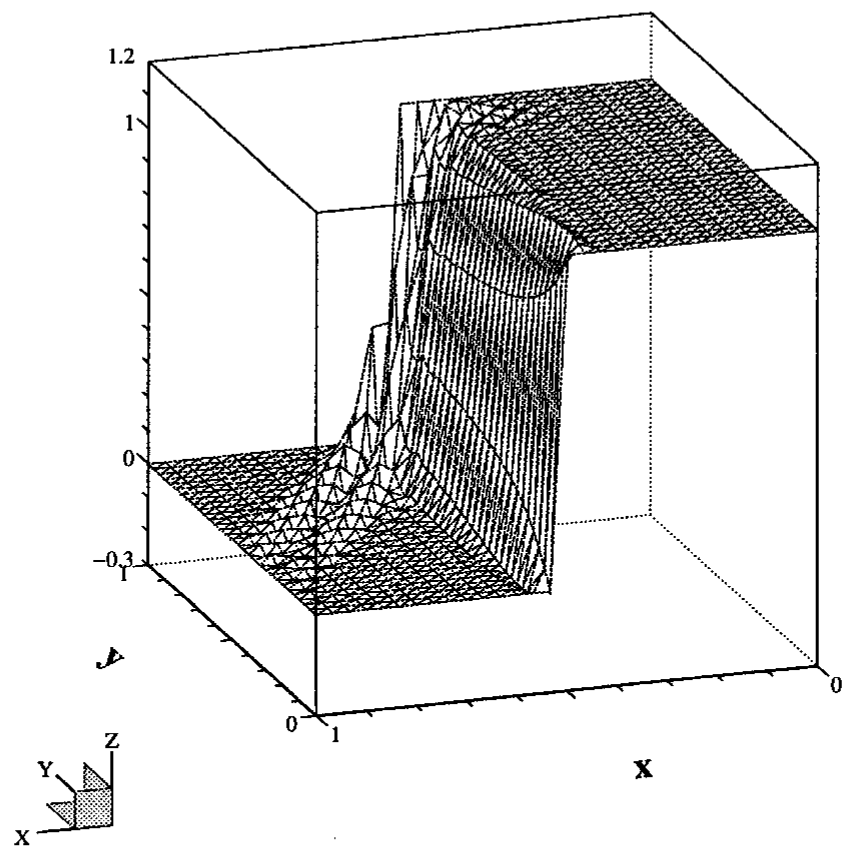
\includegraphics[width=.465\paperwidth]{images/fig-8-3-1.png}
  \caption{用 Galerkin 法得到的数值结果}\label{fig:8.3.1}
\end{figure}

注意,对于问题\eqref{eq:8.3.3},对流项对稳定性估计不起作用.因此,无法得到与参数 \(\varepsilon\) 无关的先验控制.

前面已经表明,一种可能的补救措施是采用 Petrov--Galerkin 逼近.在一维情形,它等价于迎风有限差分格式.不过,这种方法引入了 \(O(h)\) 量级的数值黏性,影响了逼近精度.

下面回顾几种用于逼近 \(d\) 维问题\eqref{eq:8.3.1}的方法.首先介绍具有一阶精度的人工扩散法,随后着重讨论几种具有强相容性(见\eqref{eq:8.3.6})和高阶精度的稳定化方法.

\subsection{人工扩散法}\label{sec:8.3.1}
\SourcePage{277}

经典的\emph{人工扩散法}是一维迎风有限差分格式在 \(d\) 维情形下的推广.它在所有方向上引入 \(O(h)\) 量级的数值扩散.

这一方法的思想很容易解释.Galerkin 法在 Péclet 数 \(\mathrm{Pe}\) 较大时会产生振荡,此时椭圆性常数 \(\alpha_0\) 相对于 \(\|\boldsymbol{b}\|_{L^\infty(\Omega)}\) 与 \(h\) 的乘积很小.为避免这一困难,可将原问题改为椭圆性常数更大的问题.例如,在 \(L\) 上加上算子 \(\mathcal L\),其中
\[
  \mathcal Lz:=-hQ\Delta z,\qquad Q:=\|\boldsymbol{b}\|_{L^\infty(\Omega)}.
\]
椭圆性常数变为 \(\alpha_0^*:=\alpha_0+hQ\).对新算子应用 Galerkin 法,得到不再受振荡影响的近似解.

新的解 \(u_h^*\) 满足
\begin{equation}\label{eq:8.3.4}
  u_h^*\in V_h:\quad a_h(u_h^*,v_h)=(f,v_h)\qquad\forall\,v_h\in V_h,
\end{equation}
其中
\[
  a_h(z,v):=a(z,v)+hQ(\nabla z,\nabla v)\qquad\forall\,z,v\in V.
\]
这是一个广义 Galerkin 问题(见第~\ref{sec:5.5}~节).

这种处理有一个明显的缺点.由于附加项 \(-hQ\Delta z\) 为 \(O(h)\) 量级,特别有
\begin{equation}\label{eq:8.3.5}
  \sup_{\substack{v_h\in V_h\\v_h\ne0}}
     \frac{|a_h(u,v_h)-(f,v_h)|}{\|v_h\|_1}=O(h),
\end{equation}
其中 \(u\) 是\eqref{eq:8.3.1}的解.这说明格式是\emph{相容}的,但只有一阶相容性.因此,无论有限元空间的多项式次数 \(k\) 有多高,人工扩散法的精度都不会超过一阶.

对于最低次的分片线性有限元(\(k=1\)),上述稳定化仍能保持误差 \(H^1\) 范数下的一阶精度,但会使误差的最大范数从 \(O(h^2|\log h|)\)(见笔记~\ref{note:6.2.3})退化到 \(O(h)\).

因此,稳定项与多项式逼近本来可以保证的最优阶不相容.采用谱方法时,精度损失更加明显.

应用命题~\ref{pro:5.5.1}可得到人工扩散法的误差估计.具体来说,
\[
  \|u-u_h^*\|_1\le C\left(\inf_{v_h\in V_h}\|u-v_h\|_1+h\|u\|_1\right),
\]
\SourcePage{278}其中 \(C=C(\alpha,\gamma,Q)\),而 \(\alpha\) 和 \(\gamma\) 分别是双线性形式 \(a(\cdot,\cdot)\) 的强制性常数和连续性常数.

和一维迎风有限差分的情形一样,稳定性的获得以精度损失为代价.典型结果会表现出过度扩散,\figref{fig:8.2.1}已经给出了一维的情形.在二维情形,除了沿流线方向(即与 \(\boldsymbol{b}(\boldsymbol{x})\) 方向平行的曲线方向)有扩散,在与之垂直的方向上也可观察到扩散.这种不希望出现的现象通常称为\emph{横风扩散},见\figref{fig:8.3.2}.

\begin{figure}[!htbp]
  \centering
  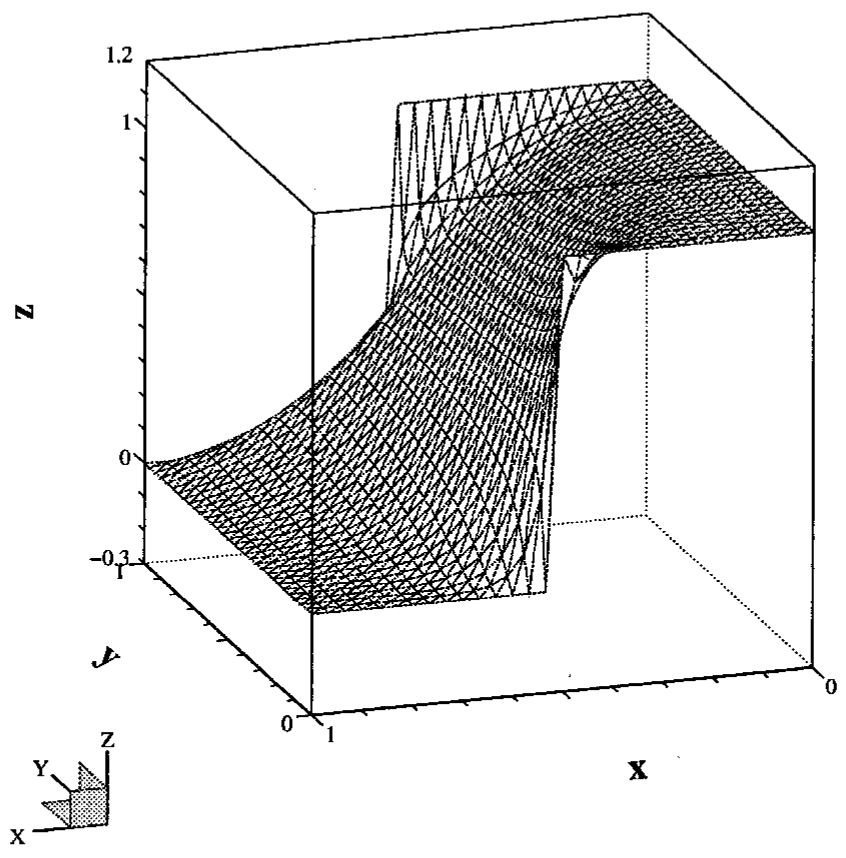
\includegraphics[width=.461\paperwidth]{images/fig-8-3-2.png}
  \caption{用人工扩散法得到的数值结果}\label{fig:8.3.2}
\end{figure}

可以在 \(L\) 上加上如下算子 \(\widehat{\mathcal L}\) 来避免横风扩散：
\[
  \widehat{\mathcal L}z:=-\frac hQ\operatorname{div}
       [(\boldsymbol{b}\cdot\nabla z)\boldsymbol{b}].
\]
它在 \(H_0^1(\Omega)\) 上不具有强制性,但满足
\[
  \int_\Omega(\widehat{\mathcal L}v)v=\frac hQ\int_\Omega(\boldsymbol{b}\cdot\nabla v)^2
    \ge0\qquad\forall\,v\in H_0^1(\Omega).
\]
这一做法称为\emph{流线迎风法}.在有限差分格式中由\BookCite{raithby1976}{Raithby(1976)}提出,在有限元框架下由\BookCite{hughes-brooks1979}{Hughes 和 Brooks(1979)}提出.它产生的人工扩散只沿流线方向影响近似解.\SourcePage{279}不过,它仍引入一阶附加项,所以只有 \(O(h)\) 精度.

\begin{note}\NumberedNote{note:8.3.1}
文献中还提出了其他几种迎风型有限元法.下一小节将介绍不同作者提出的一族稳定化方法.关于较早格式的理论介绍和计算效率分析,见\BookCite{ikeda1983}{Ikeda(1983)}、\BookCite{tabata1986}{Tabata(1986)}及其中所引文献.\hfill\(\square\)
\end{note}

\subsection{有限元的强相容稳定化方法}\label{sec:8.3.2}

本小节介绍几种能保持多项式子空间固有精度的稳定化方法.这些方法都属于\eqref{eq:5.5.1}所述的广义 Galerkin 法.若 \(u\) 是问题\eqref{eq:8.3.1}的精确解,则有
\begin{equation}\label{eq:8.3.6}
  \mathcal A_h(u,v_h)-\mathcal F_h(v_h)=0\qquad\forall\,v_h\in V_h.
\end{equation}
这个性质加强了相容性\eqref{eq:8.3.5},称为\emph{强相容性}.它使稳定化方法能够保持由有限维子空间的选取所决定的最优精度.

下面会看到,即使 Péclet 数很大,这些方法仍能给出无振荡的解.某些数值扩散依然存在,但主要沿流线方向影响解,使横风扩散明显减弱.

此外,适当调整这些方法,也可以用来处理其他问题中的不同类型的数值病态.例如,在 Stokes 问题的逼近中,不稳定性来自伪压力模态.若速度和压力的逼近子空间之间不满足适当的相容性条件,就可能出现这类模态(见第~\BookRef{sec:9.2}{9.2}~节和第~\BookRef{sec:9.4}{9.4}~节).

考察\eqref{eq:8.1.1}引入的算子 \(L\),按 \(L^2(\Omega)\) 的内积将它分解为对称部分和斜对称部分,即
\begin{equation}\label{eq:8.3.7}
  L=L_S+L_{SS},
\end{equation}
其中
\SourcePage{280}
\begin{align}
  L_S z&:=-\sum_{i,j=1}^d D_i(a_{ij}^S D_jz)
              +\left(\frac12\operatorname{div}\boldsymbol{b}+a_0\right)z,\label{eq:8.3.8}\\
  L_{SS} z&:=-\sum_{i,j=1}^d D_i(a_{ij}^{SS}D_jz)
        +\frac12\operatorname{div}(\boldsymbol{b}z)+\frac12\boldsymbol{b}\cdot\nabla z,\label{eq:8.3.9}
\end{align}
并且
\begin{equation}\label{eq:8.3.10}
  a_{ij}^S:=\frac{a_{ij}+a_{ji}}2,\qquad
  a_{ij}^{SS}:=\frac{a_{ij}-a_{ji}}2,\qquad i,j=1,\ldots,d.
\end{equation}

取 \(\overline\Omega\) 的一族正则剖分 \(\mathcal T_h\)(见定义~\ref{def:3.4.1}),并考察由分片光滑函数组成的有限维子空间 \(V_h\subset V=H_0^1(\Omega)\).例如,可以选取 \(V_h=X_h^k\cap H_0^1(\Omega)\)、\(k\ge1\),其中 \(X_h^k\) 是\eqref{eq:3.2.4}或\eqref{eq:3.2.5}定义的有限元空间.

本章讨论\emph{对流占优情形},即假设每个 \(K\in\mathcal T_h\) 上的局部 Péclet 函数 \(\mathrm{Pe}_K(\boldsymbol{x})\) 大于 \(1\)：
\begin{equation}\label{eq:8.3.11}
  \mathrm{Pe}_K(\boldsymbol{x}):=
    \frac{|\boldsymbol{b}(\boldsymbol{x})|h_K}{2\alpha_0(\boldsymbol{x})}>1
    \qquad\forall\,\boldsymbol{x}\in K,
\end{equation}
其中
\begin{equation}\label{eq:8.3.12}
  \alpha_0(\boldsymbol{x}):=\min_{\boldsymbol{\xi}\in\mathbb R^d\setminus\{0\}}
    \frac{\sum_{i,j=1}^d a_{ij}(\boldsymbol{x})\xi_i\xi_j}{|\boldsymbol{\xi}|^2},
      \qquad \boldsymbol{x}\in\overline\Omega.
\end{equation}
这里及下文均假设系数 \(a_{ij}(\boldsymbol{x})\) 和 \(\boldsymbol{b}(\boldsymbol{x})\) 在 \(\overline\Omega\) 上连续.注意,由椭圆性假设(见定义~\ref{def:6.1.1}),对于每个 \(\boldsymbol{x}\in\overline\Omega\),都有 \(\alpha_0(\boldsymbol{x})\ge\alpha_0>0\).此外,\eqref{eq:8.3.11}特别蕴含 \(\inf_\Omega|\boldsymbol{b}(\boldsymbol{x})|>0\).

现在可以引入\eqref{eq:8.3.1}的\emph{稳定化逼近}.定义
\[
  \begin{aligned}
    \mathcal L_h^{(\rho)}(z_h,v_h)
      &:=\sum_{K\in\mathcal T_h}\delta\left(
           Lz_h,\frac{h_K}{|\boldsymbol{b}|}(L_{SS}+\rho L_S)v_h\right)_K,\\
    \varphi_h^{(\rho)}(v_h)
      &:=\sum_{K\in\mathcal T_h}\delta\left(
           f,\frac{h_K}{|\boldsymbol{b}|}(L_{SS}+\rho L_S)v_h\right)_K,
  \end{aligned}
\]
其中 \(z_h,v_h\in V_h\),\((\cdot,\cdot)_K\) 表示 \(L^2(K)\) 的内积,参数 \(\delta>0\) 和 \(\rho\in\mathbb R\) 有待选定.于是,考虑如下问题：
\begin{equation}\label{eq:8.3.13}
  \text{求 }u_h\in V_h,\quad\text{使}\quad
     a(u_h,v_h)+\mathcal L_h^{(\rho)}(u_h,v_h)
       =(f,v_h)+\varphi_h^{(\rho)}(v_h)\qquad\forall\,v_h\in V_h.
\end{equation}
进一步,用 \(a_h^{(\rho)}(\cdot,\cdot)\) 表示上面的稳定化双线性形式,即
\SourcePage{281}
\begin{equation}\label{eq:8.3.14}
  a_h^{(\rho)}(z_h,v_h):=a(z_h,v_h)+\mathcal L_h^{(\rho)}(z_h,v_h)
     \qquad\forall\,z_h,v_h\in V_h,
\end{equation}
用 \(\mathcal F_h^{(\rho)}(\cdot)\) 表示经扰动的连续线性泛函
\[
  \mathcal F_h^{(\rho)}(v_h):=(f,v_h)+\varphi_h^{(\rho)}(v_h)\qquad\forall\,v_h\in V_h.
\]

先说明一个重要的事实.由于精确解 \(u\) 满足 \(Lu=f\in L^2(\Omega)\),对每个 \(v_h\in V_h\),\(a_h^{(\rho)}(u,v_h)\) 都有定义.此外,无论怎样选取 \(\delta\) 和 \(\rho\),问题\eqref{eq:8.3.13}都具有\eqref{eq:8.3.6}意义下的\emph{强相容性}.现在的问题是如何选取合适的参数,使得在适当范数下同时具有稳定性和收敛性.

第~\BookRef{sec:8.4}{8.4}~节将分析参数 \(\rho\) 取三个不同值时的稳定化问题\eqref{eq:8.3.13}.这些方法分别由不同的研究者提出.这里沿用\BookCite{baiocchi-brezzi1992}{Baiocchi 和 Brezzi(1992)}的做法,将它们放在统一的框架下介绍.\(\rho=0\) 对应 \emph{SUPG 法(流线迎风/Petrov--Galerkin 法)},由\BookCite{hughes-brooks1982}{Hughes 和 Brooks(1982)}及\BookCite{brooks-hughes1982}{Brooks 和 Hughes(1982)}提出.这一方法也称为\emph{流线扩散法},例如见\BookCite{johnson1987}{Johnson(1987)}.\(\rho=1\) 对应 \emph{GALS 法(Galerkin/最小二乘法)},由\BookCite{hughes-franca-hulbert1989}{Hughes、Franca 和 Hulbert(1989)}引入.\(\rho=-1\) 对应\BookCite{franca-frey-hughes1992}{Franca、Frey 和 Hughes(1992)}提出的方法,它将\BookCite{douglas-wang1989}{Douglas 和 Wang(1989)}在 Stokes 问题逼近中使用的思想推广到对流--扩散方程.称最后这一种为 \emph{DWG 法(Douglas--Wang/Galerkin 法)}.应当注意,当扩散系数在各单元上为常数、\(\tfrac12\operatorname{div}\boldsymbol{b}+a_0=0\) 且以分片线性多项式作为试验函数时,上述三种方法一致.

\begin{note}\NumberedNote{note:8.3.2}
如前所述,SUPG 是流线迎风/Petrov--Galerkin 的缩写.不过,正如\BookCite{hughes1987}{Hughes(1987)}指出的,这一名称未必恰当.实际上,SUPG 是\eqref{eq:8.3.13}的特例,而\eqref{eq:8.3.13}是广义 Galerkin 法.\hfill\(\square\)
\end{note}

\begin{note}\NumberedNote{note:8.3.3}
在{\heiti 扩散占优情形},即对每个 \(K\in\mathcal T_h\) 和每个 \(\boldsymbol{x}\in K\) 都有 \(\mathrm{Pe}_K(\boldsymbol{x})\le1\) 时,标准 Galerkin 法就能令人满意地处理这一问题.不过,只要将稳定化参数 \(\delta\) 取为 \(\mathrm{Pe}_K\) 的函数,具体取 \(\delta=O(\mathrm{Pe}_K)\),也可使用\eqref{eq:8.3.13}的稳定化方法(另见笔记~\BookRef{note:8.4.2}{8.4.2}).\hfill\(\square\)
\end{note}

最后给出一些数值结果.先用稳定化 GALS 法和分片二次有限元逼近对流--扩散方程\eqref{eq:8.3.3},其中取 \(\varepsilon=10^{-5}\).剖分采用 \(30\times30\) 个均匀分布的节点.选取几种不同的对流场 \(\boldsymbol{b}\) 和 \(u\) 的边界值.每个算例中的\SourcePage{282}\(\boldsymbol{b}\) 及边界数据都可以直接从下面的图中看出.\figref{fig:8.3.3}\subref{fig:8.3.3a} 和 \subref{fig:8.3.3b} 表明,数值耗散只能沿流线方向增加.图 \subref{fig:8.3.3a} 中完全没有耗散,图 \subref{fig:8.3.3b} 中则由于流线穿过间断线而出现扩散.后一情形下还可看到一些欠冲和过冲,这在此类稳定化方法中时常发生(另见\figref{fig:8.3.3}\subref{fig:8.3.3c}).图 \subref{fig:8.3.3c} 和 \subref{fig:8.3.3d} 对应的测试问题实际上相同.不过,图 \subref{fig:8.3.3d} 表明,网格取向可能产生显著影响,导致即使 \(\boldsymbol{b}\) 与间断线平行,也出现数值扩散.

层附近出现的欠冲与过冲说明格式缺乏单调性.可在\eqref{eq:8.3.13}中再引入一个稳定项来克服这一缺陷.所加的是一个激波捕捉型非线性黏性项,见\BookCite{hughes-mallet-mizukami1986}{Hughes、Mallet 和 Mizukami(1986)}、\BookCite{galeao-dutradocarmo1988}{Galeão 和 Dutra do Carmo(1988)}、\BookCite{shakib1988}{Shakib(1988)}.

\begin{figure}[!htbp]
  \centering
  \caption{用 GALS 法得到的数值结果}\label{fig:8.3.3}
  \begin{subfigure}{\linewidth}
    \centering
    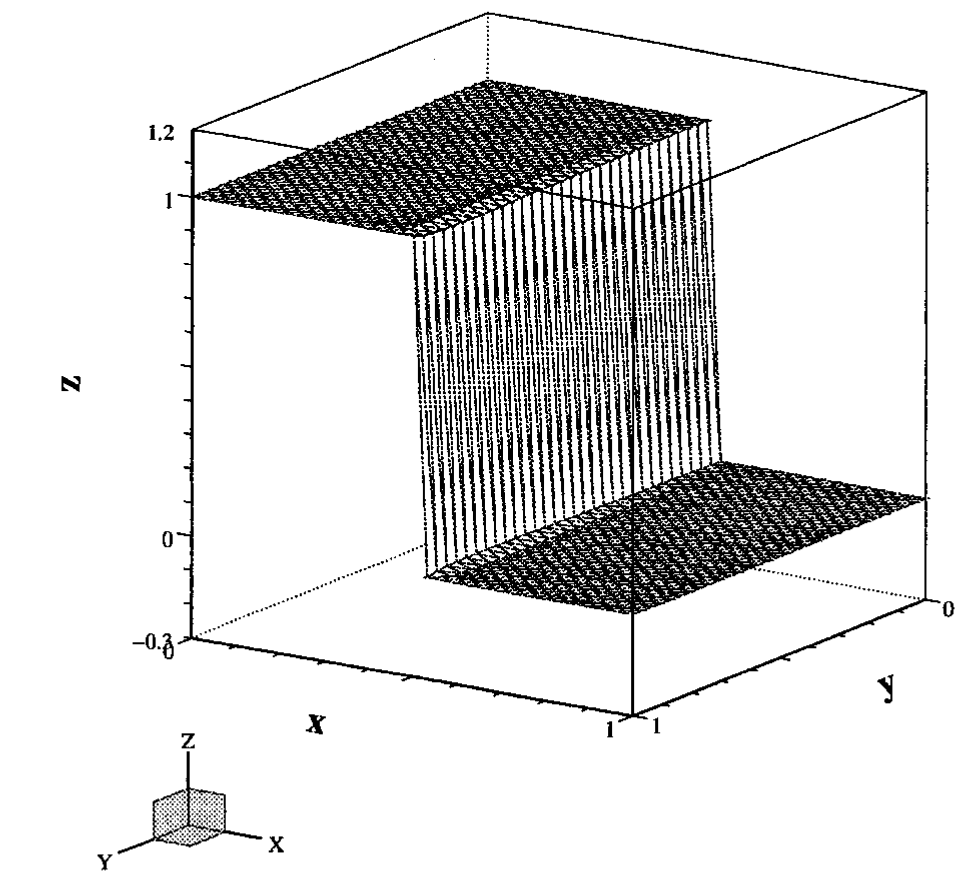
\includegraphics[width=.527\paperwidth]{images/fig-8-3-3a.png}
    \caption{}\label{fig:8.3.3a}
  \end{subfigure}\par\medskip
  \begin{subfigure}{\linewidth}
    \centering
    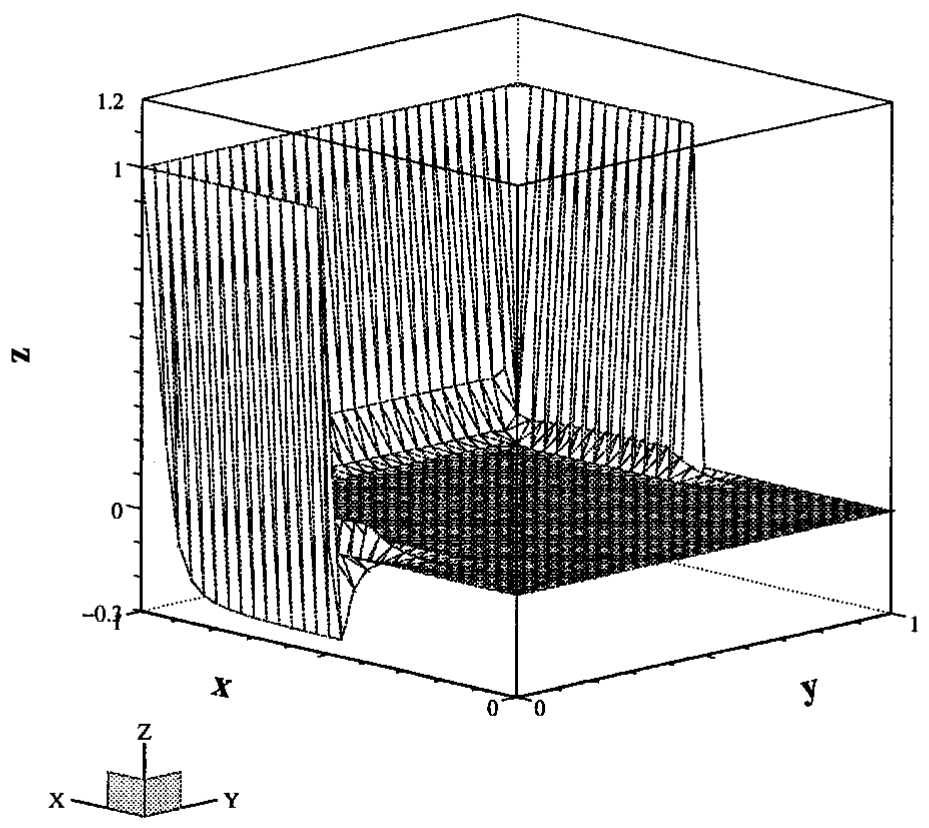
\includegraphics[width=.507\paperwidth]{images/fig-8-3-3b.png}
    \caption{}\label{fig:8.3.3b}
  \end{subfigure}
\end{figure}
\begin{figure}[!htbp]
  \ContinuedFloat
  \centering
  \caption[]{用 GALS 法得到的数值结果(续)}
  \begin{subfigure}{\linewidth}
    \centering
    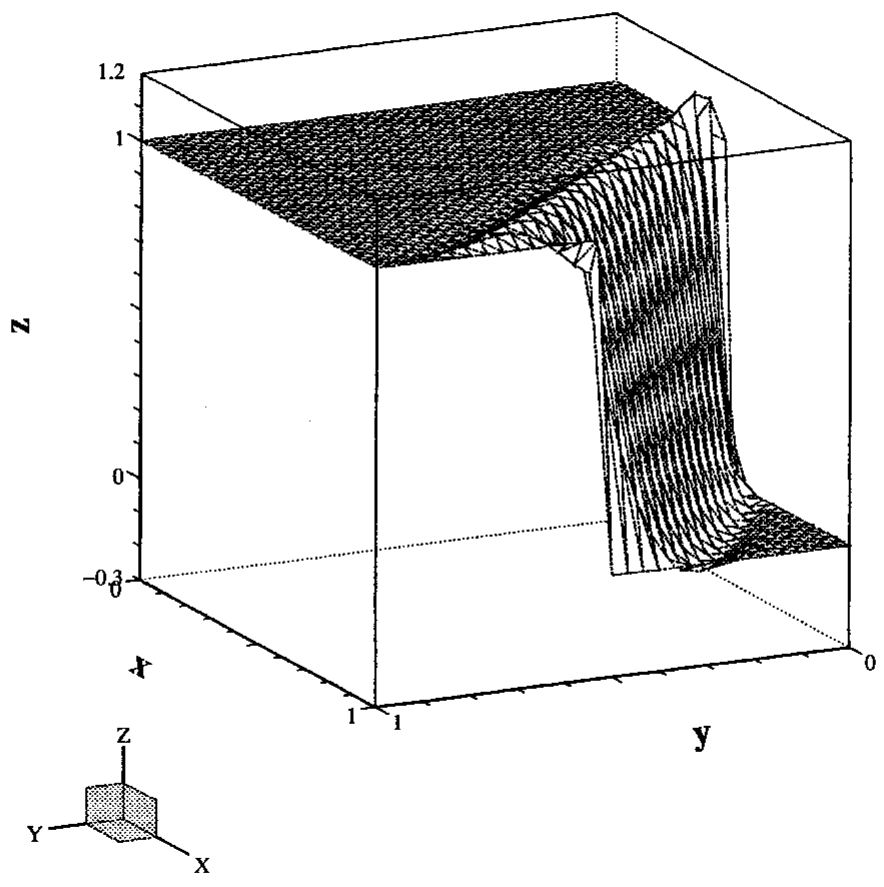
\includegraphics[width=.483\paperwidth]{images/fig-8-3-3c.png}
    \caption{}\label{fig:8.3.3c}
  \end{subfigure}\par\medskip
  \begin{subfigure}{\linewidth}
    \centering
    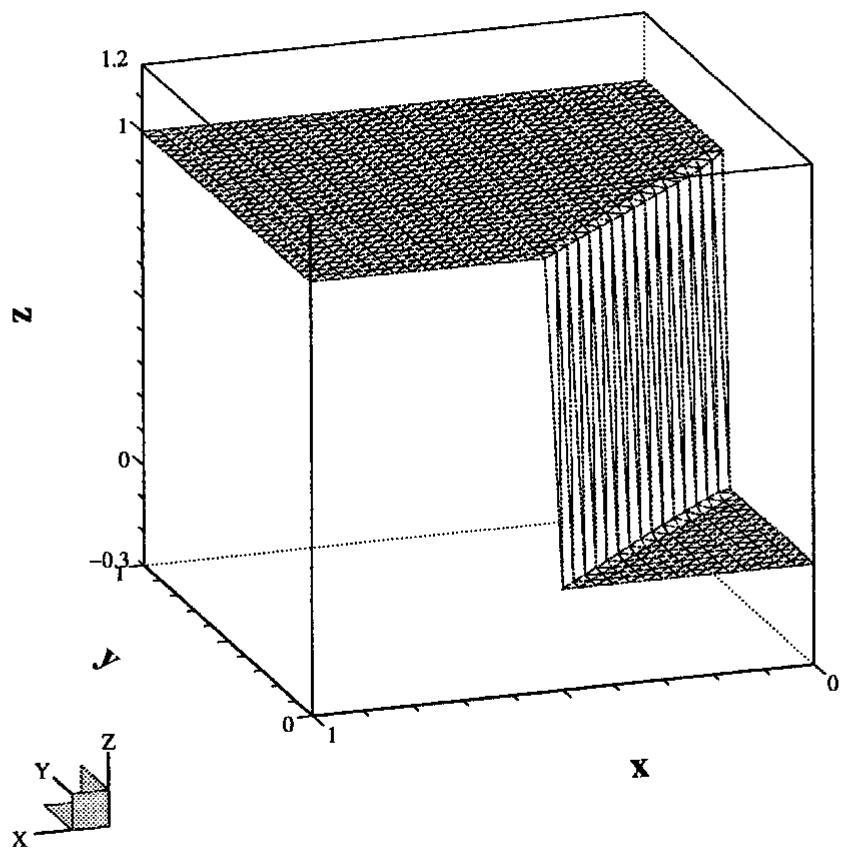
\includegraphics[width=.461\paperwidth]{images/fig-8-3-3d.png}
    \caption{}\label{fig:8.3.3d}
  \end{subfigure}
\end{figure}

\clearpage
\subsection{利用泡函数稳定化}\label{sec:8.3.3}
\SourcePage{283}

在分析上一小节所给方法的稳定性和收敛性之前,先介绍另一种解释.最早的解释由\BookCite{brezzi-bristeau-franca-mallet-roge1992}{Brezzi、Bristeau、Franca、Mallet 和 Rogé(1992)}给出.进一步的说明和改进见\BookCite{baiocchi-brezzi-franca1993}{Baiocchi、Brezzi 和 Franca(1993)}.关于不同背景下的类似方法,另见笔记~\BookRef{note:9.4.2}{9.4.2}.

为简便起见,仅考虑二维情形,即 \(d=2\).先引入有限维空间
\begin{equation}\label{eq:8.3.15}
  V_h^b:=[X_h^k\cap H_0^1(\Omega)]\oplus B,
\end{equation}
其中 \(X_h^k\) 按\eqref{eq:3.2.4}定义,\(B\) 是由\emph{泡函数}组成的有限维空间,在每个单元 \(K\in\mathcal T_h\) 上恰有一个自由度.例如,若 \(k<3\),可以选用三次泡函数,即
\begin{equation}\label{eq:8.3.16}
  B=B_3:=\{v_B\in H_0^1(\Omega)\mid
       v_B|_K=c_Kb_K,\ c_K\in\mathbb R,\ b_K=\lambda_1\lambda_2\lambda_3
       \quad\forall\,K\in\mathcal T_h\}.
\end{equation}
这里的 \(\lambda_i\)(\(i=1,2,3\))为线性多项式,各自在 \(K\) 的一条边上为零,并在对顶点取值 \(1\).因此,泡函数的一个例子 \(b_K\) 在 \(K\) 的内部为正,在 \(\partial K\) 上为零.

现在考察\eqref{eq:8.3.1}在 \(V_h^b\) 中的 Galerkin 逼近：
\SourcePage{284}
\begin{equation}\label{eq:8.3.17}
  \begin{aligned}
    \text{求 }u_h+u_B\in V_h^b,\quad\text{使}\quad
      a(u_h+u_B,v_h+v_B)&=(f,v_h+v_B)\\
      &\qquad\forall\,v_h+v_B\in V_h^b.
  \end{aligned}
\end{equation}
我们想先求出 \(u_B\),再将\eqref{eq:8.3.17}改写成 \(X_h^k\cap H_0^1(\Omega)\) 中的稳定化 Galerkin 法.首先,在每个 \(K\) 上可以将 \(u_B\) 写成
\begin{equation}\label{eq:8.3.18}
  u_B|_K=c_{b,K}b_K.
\end{equation}
在\eqref{eq:8.3.17}中,选试验函数 \(v_h=0\) 和 \(v_B\in B\),其中
\[
  v_B=
  \begin{cases}
    b_K,&\text{在 }K\text{ 内},\\
    0,&\text{在 }\Omega\setminus K\text{ 上},
  \end{cases}
\]
便有
\[
  a(u_h+u_B,v_B)=a_K(u_h+c_{b,K}b_K,b_K),
\]
其中 \(a_K(\cdot,\cdot)\) 表示 \(a(\cdot,\cdot)\) 在三角形 \(K\) 上的限制.于是,\eqref{eq:8.3.17}成为
\[
  a_K(u_h,b_K)+c_{b,K}a_K(b_K,b_K)=(f,b_K)_K.
\]
由于 \(u_h|_K\) 是多项式且 \(b_K\) 在 \(\partial K\) 上为零,可以对第一项分部积分,得到
\begin{equation}\label{eq:8.3.19}
  c_{b,K}=\frac{(f-Lu_h,b_K)_K}{a_K(b_K,b_K)}.
\end{equation}

\SourcePage{285}现在在\eqref{eq:8.3.17}中选任意 \(v_h\in X_h^k\cap H_0^1(\Omega)\) 和 \(v_B=0\) 作为试验函数,得到
\[
  a(u_h,v_h)+\sum_{K\in\mathcal T_h}c_{b,K}a_K(b_K,v_h)=(f,v_h).
\]
分部积分后,\(a_K(b_K,v_h)\) 一项给出
\[
  a_K(b_K,v_h)=(b_K,L_Sv_h-L_{SS}v_h)_K
\]
(记号见\eqref{eq:8.3.8}和\eqref{eq:8.3.9}).同理,
\[
  a_K(b_K,b_K)=(L_Sb_K,b_K)_K.
\]
利用\eqref{eq:8.3.19},最终可将\eqref{eq:8.3.17}写成
\begin{equation}\label{eq:8.3.20}
  a(u_h,v_h)+a_B(f;u_h,v_h)=(f,v_h)\qquad\forall\,v_h\in X_h^k\cap H_0^1(\Omega),
\end{equation}
其中
\begin{equation}\label{eq:8.3.21}
  a_B(f;u_h,v_h):=\sum_{K\in\mathcal T_h}
      \frac{(Lu_h-f,b_K)_K(L_{SS}v_h-L_Sv_h,b_K)_K}{(L_Sb_K,b_K)_K}.
\end{equation}
\eqref{eq:8.3.1}的这一有限维逼近具有强相容性.与通常的 Galerkin 逼近相比,它多出附加项 \(a_B(f;u_h,v_h)\).此外,它与\eqref{eq:8.3.13}中 \(\rho=-1\) 时的 DWG 法相似,因为 DWG 法的附加项形如
\SourcePage{286}
\begin{equation}\label{eq:8.3.22}
  \sum_{K\in\mathcal T_h}\delta\left(
     Lu_h-f,\frac{h_K}{|\boldsymbol{b}|}(L_{SS}v_h-L_Sv_h)\right)_K.
\end{equation}

下面说明,至少在一种简化情形下,可以将\eqref{eq:8.3.21}写成\eqref{eq:8.3.22}的形式.取\eqref{eq:3.2.4}中的分片线性有限元(\(k=1\)).假设 \(\boldsymbol{b}(\boldsymbol{x})\) 为常向量、\(f(\boldsymbol{x})\) 为常数、\(a_0(\boldsymbol{x})=0\),且 \(a_{ij}(\boldsymbol{x})=\varepsilon\delta_{ij}\),其中 \(\varepsilon>0\) 为常数,\(\delta_{ij}\) 是 Kronecker 符号.这时,
\[
  L_Sz=-\varepsilon\Delta z,\qquad L_{SS}z=\boldsymbol{b}\cdot\nabla z,
\]
SUPG、GALS 和 DWG 法均一致.再按\eqref{eq:8.3.16}选取泡函数空间 \(B\).注意,泡函数 \(b_K\) 满足
\begin{equation}\label{eq:8.3.23}
  \int_Kb_K=C_1\operatorname{meas}(K)=C_{1,K}h_K^2,\qquad
    \int_K|\nabla b_K|^2=C_{2,K},
\end{equation}
其中常数 \(C_{1,K}\) 和 \(C_{2,K}\) 与 \(h_K\) 无关.

先计算 \((Lu_h-f,b_K)_K\).回顾 \(u_h|_K\in\mathbb P_1\),由\eqref{eq:8.3.23}有
\[
  \begin{aligned}
    (Lu_h-f,b_K)_K
      &=(\boldsymbol{b}\cdot\nabla u_h-f,b_K)_K
       =(\boldsymbol{b}\cdot\nabla u_h|_K-f)\int_K b_K\\
      &=(\boldsymbol{b}\cdot\nabla u_h|_K-f)C_{1,K}h_K^2.
  \end{aligned}
\]
同样,
\[
  (L_{SS}v_h-L_Sv_h,b_K)_K=(\boldsymbol{b}\cdot\nabla v_h,b_K)_K
    =(\boldsymbol{b}\cdot\nabla v_h|_K)C_1\operatorname{meas}(K).
\]
最后,由\eqref{eq:8.3.23}得
\[
  (L_Sb_K,b_K)_K=-\varepsilon(\Delta b_K,b_K)_K=\varepsilon C_{2,K}.
\]
因此可写成
\[
  \begin{aligned}
    a_B(f;u_h,v_h)
      &=\sum_{K\in\mathcal T_h}
        \frac{(\boldsymbol{b}\cdot\nabla u_h|_K-f)(\boldsymbol{b}\cdot\nabla v_h|_K)
             C_1C_{1,K}h_K^2\operatorname{meas}(K)}{\varepsilon C_{2,K}}\\
      &=\sum_{K\in\mathcal T_h}
        \frac{C_1C_{1,K}h_K^2}{\varepsilon C_{2,K}}(L_{SS}u_h-f,L_{SS}v_h)_K.
  \end{aligned}
\]
再由定义\eqref{eq:8.3.11}最终得到
\begin{equation}\label{eq:8.3.24}
  a_B(f;u_h,v_h)=\sum_{K\in\mathcal T_h}\frac{2C_1C_{1,K}\mathrm{Pe}_K}{C_{2,K}}
      \left(Lu_h-f,\frac{h_K}{|\boldsymbol{b}|}(L_{SS}v_h-L_Sv_h)\right)_K.
\end{equation}

\SourcePage{287}与\eqref{eq:8.3.13}比较便可看出,泡函数带来的附加项恰好是 DWG 法的稳定项,其中在每个单元 \(K\in\mathcal T_h\) 上适当选取常数 \(\delta=\delta_K\).再次注意,在当前假设下,\(L_Su_h=L_Sv_h=0\),所以 SUPG、GALS 和 DWG 法一致.

实际上,\eqref{eq:8.3.24}用于对流占优问题的逼近时还不够理想,因为常数 \(\delta_K:=2C_{2,K}^{-1}C_1C_{1,K}\mathrm{Pe}_K\) 依赖于局部 Péclet 数.不过,稍稍改变做法并选用其他类型的泡函数,就能得到形式\eqref{eq:8.3.13},其中参数 \(\delta_K\) 与 \(\mathrm{Pe}_K\) 无关.见\BookCite{brezzi-bristeau-franca-mallet-roge1992}{Brezzi、Bristeau、Franca、Mallet 和 Rogé(1992)}.

\subsection{谱逼近的稳定化方法}\label{sec:8.3.4}

本小节考察谱配置逼近的两种稳定化方法.第一种方法表明,在标准谱配置格式中增加具有局部支集的近似解基函数和试验函数(通常为泡函数),可以使格式稳定.第二种方法将第~\ref{sec:8.3.2}~节的方法推广到谱配置,在通常的 Galerkin 方法中加入与 SUPG、GALS 或 DWG 法类似的附加项.

为简便起见,集中讨论二维齐次 Dirichlet 问题
\begin{equation}\label{eq:8.3.25}
  \begin{cases}
    Lu:=-\varepsilon\Delta u+\operatorname{div}(\boldsymbol{b}u)+a_0u=f,
       &\text{在 }\Omega\text{ 内},\\
    u=0,&\text{在 }\partial\Omega\text{ 上},
  \end{cases}
\end{equation}
其中 \(f\in L^2(\Omega)\)、\(\Omega=(-1,1)^2\).与\eqref{eq:8.3.25}对应的双线性形式 \(a(\cdot,\cdot)\) 按\eqref{eq:8.1.2}定义,其中 \(a_{ij}=\varepsilon\delta_{ij}\).假设它连续且具有强制性,即满足\eqref{eq:8.1.3}和\eqref{eq:8.1.4}.相应的变分问题为
\begin{equation}\label{eq:8.3.26}
  \text{求 }u\in H_0^1(\Omega),\quad\text{使}\quad
    a(u,v)=(f,v)\qquad\forall\,v\in H_0^1(\Omega).
\end{equation}

对每个整数 \(N\ge2\),Legendre--Gauss--Lobatto 节点 \(\boldsymbol{x}_{ij}=(x_i,x_j)\)(\(i,j=0,\ldots,N\))诱导 \(\overline\Omega\) 的一个剖分 \(\mathcal T_h\),由 \(N^2\) 个矩形单元 \(K_{ij}:=I_i\times I_j\) 组成.每个单元的顶点是 Gauss--Lobatto 网格上的四个相邻节点.这里取 \(I_i:=[x_{i+1},x_i]\),因为 Legendre 节点通常从右向左排序,见第~\ref{sec:4.4.2}~节.仍以 \(w_{ij}\) 记 Legendre--Gauss--Lobatto 求积公式的权重(见\eqref{eq:4.5.38}).

令 \(V_N:=\mathbb Q_N^0\) 为每个变量 \(x\)、\(y\) 的次数均不超过 \(N\)、且在 \(\partial\Omega\) 上为零的多项式空间.类似地,令 \(V_h\) 为有限元空间 \(X_h^1\cap H_0^1(\Omega)\),其中 \(X_h^1\) 按\eqref{eq:3.2.5}定义.泡函数空间记为
\SourcePage{288}
\begin{equation}\label{eq:8.3.27}
  B:=\{v_B\in H_0^1(\Omega)\mid v_B|_{K_{ij}}=c_{ij}b_{ij},\
          c_{ij}\in\mathbb R,\ i,j=0,\ldots,N-1\},
\end{equation}
其中对每个 \(i,j\),预先选定一个在 \(K_{ij}\) 的边界上为零的函数 \(b_{ij}\).最简单的例子是 \(b_{ij}\in\mathbb Q_2\)、\(b_{ij}(x,y)=p_i(x)p_j(y)\),这里 \(p_i\) 和 \(p_j\) 是两个二次多项式,分别在区间 \(I_i\) 和 \(I_j\) 的两个端点处为零,在中点取值 \(1\).下文的\eqref{eq:8.3.33}给出一个更有用的选择.

沿用\BookCite{canuto1994}{Canuto(1994)}的做法,定义
\begin{equation}\label{eq:8.3.28}
  V_N^b:=V_N\oplus B,
\end{equation}
并引入\eqref{eq:8.3.26}在 \(V_N^b\) 中的 Galerkin 逼近：
\begin{equation}\label{eq:8.3.29}
  \text{求 }u_N^b\in V_N^b,\quad\text{使}\quad
    a(u_N^b,v_N^b)=(f,v_N^b)\qquad\forall\,v_N^b\in V_N^b.
\end{equation}
显然,该问题有唯一解 \(u_N^b\),且满足
\begin{align}
  \|u_N^b\|_1&\le\frac1\alpha\|f\|_0\qquad\forall\,N\ge2,\label{eq:8.3.30}\\
  \|u-u_N^b\|_1&\le\frac{\gamma}{\alpha}\inf_{v_N^b\in V_N^b}\|u-v_N^b\|_1
      \le\frac{\gamma}{\alpha}\inf_{v_N\in V_N}\|u-v_N\|_1,\label{eq:8.3.31}
\end{align}
因为 \(V_N\subset V_N^b\).这表明,该 Galerkin 逼近的先验误差界至少不劣于在 \(V_N\) 中使用标准 Galerkin 法所得的误差界.

不过,我们已经指出,谱 Galerkin 法难以实现(见第~\ref{sec:6.2.1}~节).因此,这里更关心如何给出\eqref{eq:8.3.26}的谱配置逼近.为此,假设 \(f\in C^0(\overline\Omega)\).为简便起见,再令 \(\boldsymbol{b}\) 为常向量且 \(a_0=a_0(\boldsymbol{x})\ge0\).

\BookCite{canuto1994}{Canuto(1994)}提出如下带泡函数修正的谱配置法：求 \(u_N^b=u_N+u_b\in V_N^b\),使
\begin{equation}\label{eq:8.3.32}
  \left\{
  \begin{aligned}
    (Lu_N,v_N)_N+a(u_b,\pi_h^1(v_N))
      &=(f,v_N)_N&&\forall\,v_N\in V_N,\\
    (\pi_h^1(Lu_N),v_b)+a(u_b,v_b)
      &=(\pi_h^1(f),v_b)&&\forall\,v_b\in B.
  \end{aligned}
  \right.
\end{equation}
这里,\((\cdot,\cdot)_N\) 是\eqref{eq:4.5.39}中引入的离散内积,\(\pi_h^1\colon C^0(\overline\Omega)\to X_h^1\) 是\eqref{eq:3.4.1}定义的有限元插值算子.

可以如下理解\eqref{eq:8.3.32}的由来.先按分解\eqref{eq:8.3.28}将\eqref{eq:8.3.29}分成两组方程,一组用试验函数 \(v_N\) 求 \(u_N\),另一组用试验函数 \(v_b\) 求 \(u_b\).然后,用基于 \((\cdot,\cdot)_N\) 的离散形式分别代替双线性形式 \(a(u_N,v_N)\) 和项 \((f,v_N)\).对于其余各项,用有限元插值函数逼近其中的代数多项式和 \(f\).

引入这些插值修正的目的是使整体矩阵更稀疏.事实上,\(a(u_b,\pi_h^1(v_N))\) 对应的矩阵块是带状的.\SourcePage{289}另一个矩阵块 \((\pi_h^1(Lu_N),v_b)\) 仍是满的,因为 \(Lu_N\) 依赖于 \(u_N\) 在所有网格节点上的值.不过,由于 \(\pi_h^1\) 是局部算子,这个矩阵块对 \(Lu_N\) 节点值的依赖具有带状结构.因此,可以借助\eqref{eq:8.3.32}的第二个方程逐单元用 \(Lu_N\) 在邻近节点上的值表示泡函数修正 \(u_b\),然后从第一个方程中消去 \(u_b\).

还需要说明如何构造泡函数空间 \(B\).令 \(b^*(x)\) 为区间 \((0,1)\) 上的一维泡函数,即 \(H_0^1(0,1)\) 中不恒为零的任一非负函数.于是,在每个矩形单元 \(K_{ij}=(x_{i+1},x_i)\times(x_{j+1},x_j)\) 上,令
\begin{equation}\label{eq:8.3.33}
  b_{ij}(x,y):=b^*\left(\frac{x-x_{i+1}}{x_i-x_{i+1}}\right)
    b^*\left(\frac{y-x_{j+1}}{x_j-x_{j+1}}\right).
\end{equation}
现在按\eqref{eq:8.3.27}定义空间 \(B\).

令
\[
  c^*:=\frac{\|b^*\|_0}{\|Db^*\|_0}.
\]
如果 \(c^*\) 足够小,且所需的小量与 \(N\) 无关,则问题\eqref{eq:8.3.32}有唯一解.在这种情形下,还成立
\[
  \|u_N^b\|_1\le C\|f\|_{C^0(\overline\Omega)}
\]
和
\[
  \|u-u_N^b\|_1\le C\bigl(N^{1-s}\|u\|_s+N^{-r}\|f\|_r\bigr),
\]
其中假定精确解 \(u\in H^s(\Omega)\)、\(f\in H^r(\Omega)\),且 \(s\ge1\)、\(r\ge2\).

\BookCite{pasquarelli-quarteroni1994}{Pasquarelli 和 Quarteroni(1994)}提出了另一种方法,它与第~\ref{sec:8.3.2}~节的有限元稳定化方法更为接近.现在的近似问题为：求 \(u_N\in\mathbb Q_N^0\),使
\begin{equation}\label{eq:8.3.34}
  \begin{aligned}
    (L_Nu_N,v_N+\delta(L_{N,SS}+\rho L_{N,S})v_N)_N
      &=(f,v_N+\delta(L_{N,SS}+\rho L_{N,S})v_N)_N\\
      &\qquad\forall\,v_N\in\mathbb Q_N^0,
  \end{aligned}
\end{equation}
其中 \(\delta>0\) 是一个参数,而 \(\rho\) 可以取 \(0\)(SUPG 法)、\(1\)(GALS 法)或 \(-1\)(DWG 法).这里,\(L_N\) 表示算子 \(L\) 的如下伪谱逼近：
\begin{equation}\label{eq:8.3.35}
  L_Nz:=-\varepsilon\Delta z
    +\frac12\bigl[\operatorname{div}I_N(\boldsymbol{b}z)+\boldsymbol{b}\cdot\nabla z\bigr]
    +\left(\frac12\operatorname{div}\boldsymbol{b}+a_0\right)z.
\end{equation}
显然,当 \(\boldsymbol{b}\) 为常向量且 \(z\in\mathbb Q_N\) 时,\(L_Nz=Lz\).此外,\(L_{N,S}\) 和 \(L_{N,SS}\) 分别是 \(L_N\) 关于内积 \((\cdot,\cdot)_N\) 的对称部分和斜对称部分,即
\SourcePage{290}
\begin{align}
  L_{N,S}z&:=-\varepsilon\Delta z+
      \left(\frac12\operatorname{div}\boldsymbol{b}+a_0\right)z,\label{eq:8.3.36}\\
  L_{N,SS}z&:=\frac12\bigl[\operatorname{div}I_N(\boldsymbol{b}z)
                                 +\boldsymbol{b}\cdot\nabla z\bigr].\label{eq:8.3.37}
\end{align}

和前面一样,分别记 \(\boldsymbol{x}_{ij}=(x_i,x_j)\) 和 \(w_{ij}=w_iw_j\)(\(i,j=0,\ldots,N\))为 Legendre--Gauss--Lobatto 节点和权重.\eqref{eq:8.3.34}的配置形式为
\begin{equation}\label{eq:8.3.38}
  \left\{
  \begin{aligned}
    &L_Nu_N(\boldsymbol{x}_{ij})\\
    &\quad+\delta\sum_{l,k=0}^N L_Nu_N(\boldsymbol{x}_{lk})
         (L_{N,SS}+\rho L_{N,S})\psi_{ij}(\boldsymbol{x}_{lk})\frac{w_{lk}}{w_{ij}}\\
    &\qquad=\delta\sum_{l,k=0}^N f(\boldsymbol{x}_{lk})
         (L_{N,SS}+\rho L_{N,S})\psi_{ij}(\boldsymbol{x}_{lk})\frac{w_{lk}}{w_{ij}}\\
    &\qquad\quad+f(\boldsymbol{x}_{ij})\qquad\forall\,i,j\text{ 使 }\boldsymbol{x}_{ij}\in\Omega,\\
    &u_N(\boldsymbol{x}_{ij})=0\qquad\forall\,i,j\text{ 使 }\boldsymbol{x}_{ij}\in\partial\Omega,
  \end{aligned}
  \right.
\end{equation}
其中 \(\psi_{ij}\in\mathbb Q_N^0\) 是内部节点 \(\boldsymbol{x}_{ij}\) 对应的 Lagrange 基函数.

对各 \(i,j\),函数 \((L_{N,SS}+\rho L_{N,S})\psi_{ij}\) 一般可能在各配置点都非零.因此,除边界上的方程外,每个方程都可能依赖 \(L_Nu_N\) 在所有配置点上的值.特别地,所得矩阵一般为满矩阵,区别于通常的分块矩阵(见第~\ref{sec:6.3.1}~节和第~\ref{sec:6.3.3}~节).

参数 \(\delta\) 可随配置节点而变化,也可取为常数.在后一情形,一种合适的尺度选取是
\[
  \delta=\frac{\widehat c}{\varepsilon N^4},
\]
其中 \(\widehat c>0\) 是一个与 \(\varepsilon\) 和 \(N\) 无关的待定常数.

\section{强相容稳定化方法的分析}\label{sec:8.4}

本节分析\eqref{eq:8.3.13}定义的稳定化方法.它们可视为广义 Galerkin 法,不过相应的双线性形式 \(a_h^{(\rho)}(\cdot,\cdot)\) 不满足连续性要求\eqref{eq:5.5.5},因而不适用命题~\ref{pro:5.5.1}的抽象框架.另一方面,定理~\ref{thm:5.5.1}证明的结果也不能推出这里的收敛性.

\SourcePage{291}为简便起见,下文假设存在常数 \(\mu_0\) 和 \(\mu_1\),使
\begin{equation}\label{eq:8.4.1}
  0<\mu_0\le\mu(\boldsymbol{x}):=\frac12\operatorname{div}\boldsymbol{b}(\boldsymbol{x})+a_0(\boldsymbol{x})
       \le\mu_1,\qquad \boldsymbol{x}\in\Omega.
\end{equation}
不过,如果流场 \(\boldsymbol{b}(\boldsymbol{x})\) 没有闭合流线,则可放宽这一条件.在这种情形下,较弱的条件就已足够；在 \(a_{ij}\to0\) 的极限下,甚至可以不作这一要求(例如,见\BookCite{johnson-navert-pitkaranta1984}{Johnson、Nävert 和 Pitkäranta(1984)}).

再假设系数 \(a_{ij}\) 具有如下简单形式：
\[
  a_{ij}(\boldsymbol{x})=\varepsilon\delta_{ij},\qquad
  i,j=1,\ldots,d,\quad\boldsymbol{x}\in\Omega,
\]
其中 \(\varepsilon>0\) 为常数.因此,
\[
  \begin{aligned}
    L_Sz&=-\varepsilon\Delta z+\mu z,\\
    L_{SS}z&=\tfrac12\operatorname{div}(\boldsymbol{b}z)+\tfrac12\boldsymbol{b}\cdot\nabla z,
  \end{aligned}
\]
立即得到
\begin{equation}\label{eq:8.4.2}
  a(v_h,v_h)=\varepsilon\|\nabla v_h\|_{0,\Omega}^2+
              \|\mu^{1/2}v_h\|_{0,\Omega}^2\qquad\forall\,v_h\in V_h.
\end{equation}

先分析 SUPG 法的稳定性.第一步是估计 \(a_h^{(0)}(v_h,v_h)\) 的下界.

\begin{proposition}[]{8.4.1}
假设讨论的是对流占优情形,即对每个 \(K\in\mathcal T_h\),
\begin{equation}\label{eq:8.4.3}
  \frac{|\boldsymbol{b}(\boldsymbol{x})|h_K}{2\varepsilon}>1\qquad\forall\,\boldsymbol{x}\in K.
\end{equation}
若参数 \(\delta\) 和网格尺寸 \(h_K\) 满足
\begin{equation}\label{eq:8.4.4}
  0<\delta\le C_0^{-1},\qquad
  \delta h_K\le\frac{|\boldsymbol{b}(\boldsymbol{x})|}{2\mu(\boldsymbol{x})}
             \qquad\forall\,\boldsymbol{x}\in K,
\end{equation}
其中 \(C_0\) 是下文逆不等式\eqref{eq:8.4.7}中的常数,则 SUPG 法对应的双线性形式 \(a_h^{(0)}(\cdot,\cdot)\) 满足强制性不等式
\begin{equation}\label{eq:8.4.5}
  \begin{aligned}
    a_h^{(0)}(v_h,v_h)
      &\ge\frac{\varepsilon}2\|\nabla v_h\|_{0,\Omega}^2
          +\frac12\|\mu^{1/2}v_h\|_{0,\Omega}^2\\
      &\quad+\frac12\sum_{K\in\mathcal T_h}\delta
         \left(\frac{h_K}{|\boldsymbol{b}|}L_{SS}v_h,L_{SS}v_h\right)_K
         \qquad\forall\,v_h\in V_h.
  \end{aligned}
\end{equation}
\end{proposition}

\begin{proof}
由于\eqref{eq:8.4.2}成立,只需着重考察稳定项.该项可改写为
\SourcePage{292}
\begin{equation}\label{eq:8.4.6}
  \begin{aligned}
    &\sum_{K\in\mathcal T_h}\delta
      \left(-\varepsilon\Delta v_h,\frac{h_K}{|\boldsymbol{b}|}L_{SS}v_h\right)_K\\
    &\quad+\sum_{K\in\mathcal T_h}\delta
      \left(\mu v_h,\frac{h_K}{|\boldsymbol{b}|}L_{SS}v_h\right)_K
      +\sum_{K\in\mathcal T_h}\delta
      \left(L_{SS}v_h,\frac{h_K}{|\boldsymbol{b}|}L_{SS}v_h\right)_K .
  \end{aligned}
\end{equation}
先考察第一项.下列逆不等式成立：
\begin{equation}\label{eq:8.4.7}
  \sum_{K\in\mathcal T_h}h_K^2\int_K|\Delta v_h|^2
       \le C_0\|\nabla v_h\|_{0,\Omega}^2\qquad\forall\,v_h\in V_h.
\end{equation}
证明可仿照命题~\ref{pro:6.3.2}.此外,由\eqref{eq:8.4.3}可知,在各 \(K\) 上有
\begin{equation}\label{eq:8.4.8}
  \frac{\varepsilon^2}{|\boldsymbol{b}(\boldsymbol{x})|h_K}
      \le\frac{\varepsilon}2\qquad\forall\,\boldsymbol{x}\in K.
\end{equation}
因此,
\begin{equation}\label{eq:8.4.9}
  \begin{aligned}
    &\left|\sum_{K\in\mathcal T_h}\delta
         \left(-\varepsilon\Delta v_h,\frac{h_K}{|\boldsymbol{b}|}L_{SS}v_h\right)_K\right|\\
    &\quad\le\frac14\sum_{K\in\mathcal T_h}\delta
         \left(\frac{h_K}{|\boldsymbol{b}|}L_{SS}v_h,L_{SS}v_h\right)_K
       +\sum_{K\in\mathcal T_h}\delta\varepsilon^2
         \left(\frac{h_K}{|\boldsymbol{b}|}\Delta v_h,\Delta v_h\right)_K\\
    &\quad\le\frac14\sum_{K\in\mathcal T_h}\delta
         \left(\frac{h_K}{|\boldsymbol{b}|}L_{SS}v_h,L_{SS}v_h\right)_K
       +\frac{C_0\delta\varepsilon}{2}\|\nabla v_h\|_{0,\Omega}^2.
  \end{aligned}
\end{equation}
对于\eqref{eq:8.4.6}的第二项,利用\eqref{eq:8.4.1}可作如下估计：
\begin{equation}\label{eq:8.4.10}
  \begin{aligned}
    &\left|\sum_{K\in\mathcal T_h}\delta
       \left(\mu v_h,\frac{h_K}{|\boldsymbol{b}|}L_{SS}v_h\right)_K\right|\\
    &\quad\le\frac14\sum_{K\in\mathcal T_h}\delta
         \left(\frac{h_K}{|\boldsymbol{b}|}L_{SS}v_h,L_{SS}v_h\right)_K
         +\sum_{K\in\mathcal T_h}\delta
           \left(\frac{h_K}{|\boldsymbol{b}|}\mu^2v_h,v_h\right)_K.
  \end{aligned}
\end{equation}
由\eqref{eq:8.4.2}、\eqref{eq:8.4.6}、\eqref{eq:8.4.9}和\eqref{eq:8.4.10}可得
\SourcePage{293}
\begin{equation}\label{eq:8.4.11}
  \begin{aligned}
    a_h^{(0)}(v_h,v_h)
      &\ge\varepsilon\left(1-\frac{C_0\delta}{2}\right)\|\nabla v_h\|_0^2\\
      &\quad+\frac12\sum_{K\in\mathcal T_h}\delta
           \left(\frac{h_K}{|\boldsymbol{b}|}L_{SS}v_h,L_{SS}v_h\right)_K\\
      &\quad+\sum_{K\in\mathcal T_h}
           \left(\mu\left[1-\delta\frac{h_K}{|\boldsymbol{b}|}\mu\right]v_h,v_h\right)_K.
  \end{aligned}
\end{equation}
按\eqref{eq:8.4.4}选取 \(\delta\) 和 \(h_K\),便得到稳定性不等式\eqref{eq:8.4.5}.\hfill\(\square\)
\end{proof}

注意,对于这里所考察的对流占优问题,\(|\boldsymbol{b}(\boldsymbol{x})|\) 足够大,因此\eqref{eq:8.4.4}对 \(h_K\) 的要求实际并不苛刻.

由\eqref{eq:8.4.5}可以得到问题\eqref{eq:8.3.13}的解的稳定性.为此,定义
\begin{equation}\label{eq:8.4.12}
  \begin{aligned}
    \|v_h\|_{\mathrm{SUPG}}^2
      &:=\varepsilon\|\nabla v_h\|_{0,\Omega}^2+\|\mu^{1/2}v_h\|_{0,\Omega}^2\\
      &\quad+\sum_{K\in\mathcal T_h}\delta
             \left(\frac{h_K}{|\boldsymbol{b}|}L_{SS}v_h,L_{SS}v_h\right)_K .
  \end{aligned}
\end{equation}
若 \(u_h\) 是\eqref{eq:8.3.13}在 \(\rho=0\) 时的解,则
\[
  \begin{aligned}
    \frac12\|u_h\|_{\mathrm{SUPG}}^2
      &\le a_h^{(0)}(u_h,u_h)
       =(f,u_h)+\sum_{K\in\mathcal T_h}\delta
               \left(f,\frac{h_K}{|\boldsymbol{b}|}L_{SS}u_h\right)_K\\
      &\le\|\mu^{-1/2}f\|_{0,\Omega}^2+\sum_{K\in\mathcal T_h}\delta
              \left(\frac{h_K}{|\boldsymbol{b}|}f,f\right)_K
             +\frac14\|u_h\|_{\mathrm{SUPG}}^2.
  \end{aligned}
\]
由此可知,存在与 \(h\) 无关的常数 \(C\),使
\begin{equation}\label{eq:8.4.13}
  \|u_h\|_{\mathrm{SUPG}}\le C\|f\|_{0,\Omega}.
\end{equation}
再强调一点：这个稳定性估计改进了 Galerkin 法所能得到的估计,因为其左端的范数多了附加项
\[
  \sum_{K\in\mathcal T_h}\delta
     \left(\frac{h_K}{|\boldsymbol{b}|}L_{SS}u_h,L_{SS}u_h\right)_K.
\]
特别地,这一项给出了对 \(u_h\) 沿流线方向 \(\boldsymbol{b}(\boldsymbol{x})\) 的导数的控制.

现在考察 GALS 法.由\eqref{eq:8.4.2}容易得到：

\begin{proposition}[]{8.4.2}
对任意 \(\delta>0\),GALS 法对应的双线性形式 \(a_h^{(1)}(\cdot,\cdot)\) 满足
\SourcePage{294}
\begin{equation}\label{eq:8.4.14}
  \begin{aligned}
    a_h^{(1)}(v_h,v_h)
      &=\varepsilon\|\nabla v_h\|_{0,\Omega}^2+\|\mu^{1/2}v_h\|_{0,\Omega}^2
         +\sum_{K\in\mathcal T_h}\delta
              \left(\frac{h_K}{|\boldsymbol{b}|}Lv_h,Lv_h\right)_K\\
      &=:\|v_h\|_{\mathrm{GALS}}^2\qquad\forall\,v_h\in V_h.
  \end{aligned}
\end{equation}
\end{proposition}
这一强制性性质给出一个稳定性估计.事实上,若 \(u_h\) 是\eqref{eq:8.3.13}在 \(\rho=1\) 时的解,则
\[
  \begin{aligned}
    \|u_h\|_{\mathrm{GALS}}^2
      &=a_h^{(1)}(u_h,u_h)
        =(f,u_h)+\sum_{K\in\mathcal T_h}\delta
          \left(f,\frac{h_K}{|\boldsymbol{b}|}Lu_h\right)_K\\
      &\le\|\mu^{-1/2}f\|_{0,\Omega}^2
         +\sum_{K\in\mathcal T_h}\delta\left(\frac{h_K}{|\boldsymbol{b}|}f,f\right)_K
         +\frac14\|u_h\|_{\mathrm{GALS}}^2,
  \end{aligned}
\]
因而
\begin{equation}\label{eq:8.4.15}
  \|u_h\|_{\mathrm{GALS}}\le C\|f\|_{0,\Omega}.
\end{equation}
注意,对任意选取的 \(\delta>0\),\eqref{eq:8.4.15}都成立.

为求完整,也给出 DWG 法的稳定性证明.

\begin{proposition}[]{8.4.3}
设\eqref{eq:8.4.3}成立.若参数 \(\delta\) 和网格尺寸 \(h_K\) 满足
\[
  0<\delta\le(2C_0)^{-1},\qquad
  \delta h_K\le\frac{|\boldsymbol{b}(\boldsymbol{x})|}{4\mu(\boldsymbol{x})}\qquad\forall\,\boldsymbol{x}\in K,
\]
其中 \(C_0\) 是逆不等式\eqref{eq:8.4.7}中的常数,则 DWG 法对应的双线性形式 \(a_h^{(-1)}(\cdot,\cdot)\) 满足强制性不等式
\begin{equation}\label{eq:8.4.16}
  \begin{aligned}
    a_h^{(-1)}(v_h,v_h)
      &\ge\frac{\varepsilon}2\|\nabla v_h\|_{0,\Omega}^2
       +\frac12\|\mu^{1/2}v_h\|_{0,\Omega}^2\\
      &\quad+\sum_{K\in\mathcal T_h}\delta
             \left(\frac{h_K}{|\boldsymbol{b}|}L_{SS}v_h,L_{SS}v_h\right)_K
             \qquad\forall\,v_h\in V_h.
  \end{aligned}
\end{equation}
\end{proposition}

\begin{proof}
稳定项可以改写为
\[
  \begin{aligned}
    &\sum_{K\in\mathcal T_h}\delta\left(L_{SS}v_h+L_Sv_h,
        \frac{h_K}{|\boldsymbol{b}|}(L_{SS}v_h-L_Sv_h)\right)_K\\
    &\quad=\sum_{K\in\mathcal T_h}\delta\left(\frac{h_K}{|\boldsymbol{b}|}L_{SS}v_h,L_{SS}v_h\right)_K
         -\sum_{K\in\mathcal T_h}\delta\left(\frac{h_K}{|\boldsymbol{b}|}L_Sv_h,L_Sv_h\right)_K .
  \end{aligned}
\]
\SourcePage{295}利用\eqref{eq:8.4.7}和\eqref{eq:8.4.8},可以如下估计右边第二项：
\[
  \begin{aligned}
    &\sum_{K\in\mathcal T_h}\delta\left(\frac{h_K}{|\boldsymbol{b}|}L_Sv_h,L_Sv_h\right)_K\\
    &\quad=\sum_{K\in\mathcal T_h}\delta\varepsilon^2
            \left(\frac{h_K}{|\boldsymbol{b}|}\Delta v_h,\Delta v_h\right)_K
         -2\sum_{K\in\mathcal T_h}\delta
            \left(\frac{h_K}{|\boldsymbol{b}|}\varepsilon\Delta v_h,\mu v_h\right)_K\\
    &\qquad+\sum_{K\in\mathcal T_h}\delta
             \left(\frac{h_K}{|\boldsymbol{b}|}\mu^2v_h,v_h\right)_K\\
    &\quad\le C_0\delta\varepsilon\|\nabla v_h\|_{0,\Omega}^2+
         2\sum_{K\in\mathcal T_h}\delta
             \left(\frac{h_K}{|\boldsymbol{b}|}\mu^2v_h,v_h\right)_K .
  \end{aligned}
\]
与 SUPG 的情形(见\eqref{eq:8.4.11})一样,将上式代入稳定项的下界,得到
\begin{equation}\label{eq:8.4.17}
  \begin{aligned}
    a_h^{(-1)}(v_h,v_h)
      &\ge\varepsilon(1-C_0\delta)\|\nabla v_h\|_{0,\Omega}^2\\
      &\quad+\sum_{K\in\mathcal T_h}\delta
           \left(\frac{h_K}{|\boldsymbol{b}|}L_{SS}v_h,L_{SS}v_h\right)_K\\
      &\quad+\sum_{K\in\mathcal T_h}
           \left(\mu\left[1-2\delta\frac{h_K}{|\boldsymbol{b}|}\mu\right]v_h,v_h\right)_K .
  \end{aligned}
\end{equation}
由对 \(\delta\) 和 \(h_K\) 的假设得到结论.\hfill\(\square\)
\end{proof}

显然,对于 \(\rho=-1\) 时\eqref{eq:8.3.13}的解 \(u_h\),这个结果立即给出稳定性估计\eqref{eq:8.4.13}.

现在给出\eqref{eq:8.3.13}的解 \(u_h\) 的误差估计.为简便起见,只考察 GALS 法,即\eqref{eq:8.3.13}中 \(\rho=1\) 的情形.SUPG 法和 DWG 法的收敛性可以类似地证明,有兴趣的读者可分别参见\BookCite{johnson-navert-pitkaranta1984}{Johnson、Nävert 和 Pitkäranta(1984)}及\BookCite{franca-frey-hughes1992}{Franca、Frey 和 Hughes(1992)}.

\begin{proposition}[]{8.4.4}
设空间 \(V_h\) 满足下列逼近性质：对于每个 \(v\in V\cap H^{k+1}(\Omega)\),存在 \(\widehat v_h\in V_h\),使对于每个 \(K\in\mathcal T_h\),有
\begin{equation}\label{eq:8.4.18}
  \begin{aligned}
    \|v-\widehat v_h\|_{0,K}&+h_K\|\nabla(v-\widehat v_h)\|_{0,K}
      +h_K^2\|D^2(v-\widehat v_h)\|_{0,K}\\
      &\le Ch_K^{k+1}|v|_{k+1,K}.
  \end{aligned}
\end{equation}
再假设\eqref{eq:8.4.3}成立,且 \(0<\delta\le2C_0^{-1}\),其中 \(C_0\) 是逆不等式\eqref{eq:8.4.7}中的常数.若\eqref{eq:8.1.7}的解 \(u\in H^{k+1}(\Omega)\),则它与\eqref{eq:8.3.13}在 \(\rho=1\) 时的解 \(u_h\) 满足下列估计：
\SourcePage{296}
\begin{equation}\label{eq:8.4.19}
  \|u_h-u\|_{\mathrm{GALS}}\le Ch^{k+1/2}|u|_{k+1,\Omega}.
\end{equation}
\end{proposition}

\begin{proof}
将误差写成 \(u_h-u=\sigma_h-\eta\),其中
\begin{equation}\label{eq:8.4.20}
  \sigma_h:=u_h-\widehat u_h,\qquad \eta:=u-\widehat u_h,
\end{equation}
而 \(\widehat u_h\in V_h\) 是与 \(u\) 对应、满足\eqref{eq:8.4.18}的函数.例如,若 \(V_h=X_h^k\cap H_0^1(\Omega)\),则可选取 \(\widehat u_h=\pi_h^k(u)\),其中 \(\pi_h^k\) 是\eqref{eq:3.4.1}定义的有限元插值算子(见\eqref{eq:3.4.14}).

先估计 \(\|\sigma_h\|_{\mathrm{GALS}}\).由强相容性\eqref{eq:8.3.6},
\[
  a_h^{(1)}(\sigma_h,\sigma_h)
     =a_h^{(1)}(u_h-u+\eta,\sigma_h)=a_h^{(1)}(\eta,\sigma_h).
\]
因此,利用\eqref{eq:8.4.14}得到
\begin{equation}\label{eq:8.4.21}
  \|\sigma_h\|_{\mathrm{GALS}}^2=a_h^{(1)}(\eta,\sigma_h)
       \qquad\forall\,\widehat u_h\in V_h.
\end{equation}
右端可以写成
\begin{equation}\label{eq:8.4.22}
  \begin{aligned}
    a_h^{(1)}(\eta,\sigma_h)
     &=\varepsilon\int_\Omega\nabla\eta\cdot\nabla\sigma_h
       -\int_\Omega\eta\boldsymbol{b}\cdot\nabla\sigma_h+\int_\Omega a_0\eta\sigma_h
       +\sum_{K\in\mathcal T_h}\delta\left(L\eta,\frac{h_K}{|\boldsymbol{b}|}L\sigma_h\right)_K\\
     &=\varepsilon(\nabla\eta,\nabla\sigma_h)
       -\sum_{K\in\mathcal T_h}(\eta,L\sigma_h)_K+2(\mu\eta,\sigma_h)\\
     &\quad+\sum_{K\in\mathcal T_h}(\eta,-\varepsilon\Delta\sigma_h)_K
       +\sum_{K\in\mathcal T_h}\delta\left(L\eta,\frac{h_K}{|\boldsymbol{b}|}L\sigma_h\right)_K .
  \end{aligned}
\end{equation}
逐项估计\eqref{eq:8.4.22}.首先,
\begin{equation}\label{eq:8.4.23}
  \varepsilon(\nabla\eta,\nabla\sigma_h)
     \le\frac\varepsilon4\|\nabla\sigma_h\|_{0,\Omega}^2
           +\varepsilon\|\nabla\eta\|_{0,\Omega}^2.
\end{equation}
接着,
\begin{equation}\label{eq:8.4.24}
  -\sum_{K\in\mathcal T_h}(\eta,L\sigma_h)_K
    \le\frac14\sum_{K\in\mathcal T_h}\delta
         \left(\frac{h_K}{|\boldsymbol{b}|}L\sigma_h,L\sigma_h\right)_K
        +\sum_{K\in\mathcal T_h}\left(\frac{|\boldsymbol{b}|}{\delta h_K}\eta,\eta\right)_K.
\end{equation}
第三项满足
\begin{equation}\label{eq:8.4.25}
  2(\mu\eta,\sigma_h)\le\frac12\|\mu^{1/2}\sigma_h\|_{0,\Omega}^2
                         +2\|\mu^{1/2}\eta\|_{0,\Omega}^2.
\end{equation}
\SourcePage{297}根据\eqref{eq:8.4.8},第四项可作如下估计：
\begin{equation}\label{eq:8.4.26}
  \begin{aligned}
    \sum_{K\in\mathcal T_h}(\eta,-\varepsilon\Delta\sigma_h)_K
      &\le\frac14\sum_{K\in\mathcal T_h}\delta\varepsilon^2
            \left(\frac{h_K}{|\boldsymbol{b}|}\Delta\sigma_h,\Delta\sigma_h\right)_K
        +\sum_{K\in\mathcal T_h}\left(\frac{|\boldsymbol{b}|}{\delta h_K}\eta,\eta\right)_K\\
      &\le\frac{\delta C_0\varepsilon}{8}\|\nabla\sigma_h\|_{0,\Omega}^2
        +\sum_{K\in\mathcal T_h}\left(\frac{|\boldsymbol{b}|}{\delta h_K}\eta,\eta\right)_K.
  \end{aligned}
\end{equation}
最后一项则有下列上界：
\begin{equation}\label{eq:8.4.27}
  \begin{aligned}
    \sum_{K\in\mathcal T_h}\delta\left(L\eta,\frac{h_K}{|\boldsymbol{b}|}L\sigma_h\right)_K
      &\le\frac14\sum_{K\in\mathcal T_h}\delta
               \left(\frac{h_K}{|\boldsymbol{b}|}L\sigma_h,L\sigma_h\right)_K\\
      &\quad+\sum_{K\in\mathcal T_h}\delta\left(\frac{h_K}{|\boldsymbol{b}|}L\eta,L\eta\right)_K.
  \end{aligned}
\end{equation}
综上,由于 \(0<\delta\le2C_0^{-1}\),从\eqref{eq:8.4.21}及\eqref{eq:8.4.23}至\eqref{eq:8.4.27}可得
\begin{equation}\label{eq:8.4.28}
  \begin{aligned}
    \frac12\|\sigma_h\|_{\mathrm{GALS}}^2
      &\le\varepsilon\|\nabla\eta\|_{0,\Omega}^2
          +2\sum_{K\in\mathcal T_h}\left(\frac{|\boldsymbol{b}|}{\delta h_K}\eta,\eta\right)_K\\
      &\quad+2\|\mu^{1/2}\eta\|_{0,\Omega}^2
          +\sum_{K\in\mathcal T_h}\delta\left(\frac{h_K}{|\boldsymbol{b}|}L\eta,L\eta\right)_K.
  \end{aligned}
\end{equation}
对\eqref{eq:8.4.28}的右端应用\eqref{eq:8.4.18}并利用\eqref{eq:8.4.8},最后得到
\begin{equation}\label{eq:8.4.29}
  \|\sigma_h\|_{\mathrm{GALS}}\le Ch^{k+1/2}|u|_{k+1,\Omega},\qquad u\in H^{k+1}(\Omega),
\end{equation}
其中 \(C\) 既不依赖于 \(h\),也不依赖于 \(\mathrm{Pe}_K\).不过,\(C\) 可以依赖其他一些量,例如\eqref{eq:8.4.1}中的 \(\mu_0\) 和 \(\mu_1\)、\eqref{eq:8.4.7}中的常数 \(C_0\)、\(\|\boldsymbol{b}\|_{L^\infty(\Omega)}\) 以及 \(\|a_0\|_{L^\infty(\Omega)}\).

显然,\(\|\eta\|_{\mathrm{GALS}}\) 也有类似的估计.于是,由三角不等式得到误差估计\eqref{eq:8.4.19}.\hfill\(\square\)
\end{proof}

特别地,从\eqref{eq:8.4.14}中 \(\|\cdot\|_{\mathrm{GALS}}\) 的定义可以看出,这一结果在 \(L^2(\Omega)\) 范数下给出了流线导数 \(|\boldsymbol{b}|^{-1}\boldsymbol{b}\cdot\nabla(u_h-u)\) 的最优估计,即 \(k\) 阶估计,并且关于 \(\mathrm{Pe}_K\) 一致.另一方面,\(u_h-u\) 的 \(L^2(\Omega)\) 范数为 \(O(h^{k+1/2})\),比最优阶低半阶.最后,对 \(\nabla(u_h-u)\) 的 \(L^2(\Omega)\) 范数,这个估计给出的精度至多为 \(O(h^k)\),因为由\eqref{eq:8.4.3}可知 \(\varepsilon\) 小于 \(Ch\).

\begin{note}\NumberedNote{note:8.4.1}
\BookCite{johnson-navert-pitkaranta1984}{Johnson、Nävert 和 Pitkäranta(1984)}对具有陡峭内部层和边界\SourcePage{298}层的非光滑解导出了局部化结果.这些结果表明,在这些层的一个小邻域之外,仍成立形如\eqref{eq:8.4.19}的误差估计.注意,对\eqref{eq:8.3.1}采用标准 Galerkin 法时,陡峭层的扰动效应可能沿任意方向传播,因而无法得到类似的局部估计.\hfill\(\square\)
\end{note}

\begin{note}\NumberedNote{note:8.4.2}
为简便起见,本节考察的是处处对流占优的情形\eqref{eq:8.3.11}.然而,形如\eqref{eq:8.3.13}的方法也可用于扩散占优或混合情形.若局部 Péclet 函数满足 \(\mathrm{Pe}_K(\boldsymbol{x})\le1\),便在稳定项中用 \(\delta\mathrm{Pe}_K(\boldsymbol{x})\) 代替 \(\delta h_K|\boldsymbol{b}(\boldsymbol{x})|^{-1}\)(例如,见\BookCite{hughes-franca-hulbert1989}{Hughes、Franca 和 Hulbert(1989)}以及\BookCite{franca-frey-hughes1992}{Franca、Frey 和 Hughes(1992)}).此时,方法在 GALS 范数下具有 \(O(h^k)\) 精度.\hfill\(\square\)
\end{note}

\section{若干数值结果}\label{sec:8.5}

在第~\ref{sec:8.4}~节相应的稳定性条件下,与双线性形式 \(a_h^{(\rho)}(\cdot,\cdot)\) 对应的刚度矩阵 \(A\) 正定,但不对称.因此,可采用第~\ref{sec:2.6}~节介绍的迭代方法来求解.由于 \(A\) 的条件数随网格尺寸 \(h\) 显著变化,至少在 \(h\) 较小时,预处理不可避免.

\begin{example}[对流--扩散问题的迭代收敛]\label{ex:8.5-convergence}
下面给出几幅关于对流--扩散问题\eqref{eq:8.3.3}的图,其中取 \(\boldsymbol{b}=(1,1)\),而 \(\varepsilon\ll1\) 的具体取值随后给出.解 \(u\) 的边界数据在上边 \(\{x_2=1\}\) 上取 \(1\),在 \(\{x_1=1\}\) 和 \(\{x_2=0\}\) 上取 \(0\).在边 \(\{x_1=0\}\) 上,\(0\le x_2\le1/3\) 时取 \(0\),\(1/3<x_2<2/3\) 时取 \(1/2\),\(2/3\le x_2\le1\) 时取 \(1\).沿从边 \(\{x_1=0\}\) 上两个间断点出发的特征线,解具有两个内部层.将区域剖分成 \(2n^2\) 个等面积三角形,采用分片二次有限元和 Bi-CGSTAB 迭代(见\eqref{eq:2.6.42}至\eqref{eq:2.6.53}).各图均给出归一化残差的 Euclid 范数随迭代次数的变化.

\figref{fig:8.5.1}和\figref{fig:8.5.2}对应 \(\varepsilon=10^{-2}\) 及不同的 \(n\),前者由 Galerkin 法得到,后者由 GALS 法得到.两种情形均采用 \(ILU\) 预条件矩阵(见第~\ref{sec:2.5}~节).

\figref{fig:8.5.3}和\figref{fig:8.5.4}给出 \(n=40\)、\(\varepsilon=10^{-3}\) 时的收敛过程.所用的预条件矩阵分别为对角预条件矩阵、SOR 预条件矩阵和 \(ILU\) 预条件矩阵.\figref{fig:8.5.3}对应 Galerkin 逼近,\figref{fig:8.5.4}对应 GALS 逼近.

最后,\figref{fig:8.5.5}给出 GALS 逼近在 \(n=40\) 及三种不同 \(\varepsilon\) 下的收敛过程,仍采用 \(ILU\) 预处理的 Bi-CGSTAB 迭代.由图可见,这一方法收敛很快,收敛速率实际上与 \(\varepsilon\) 无关.
\end{example}

\begin{figure}[!htbp]
  \centering
  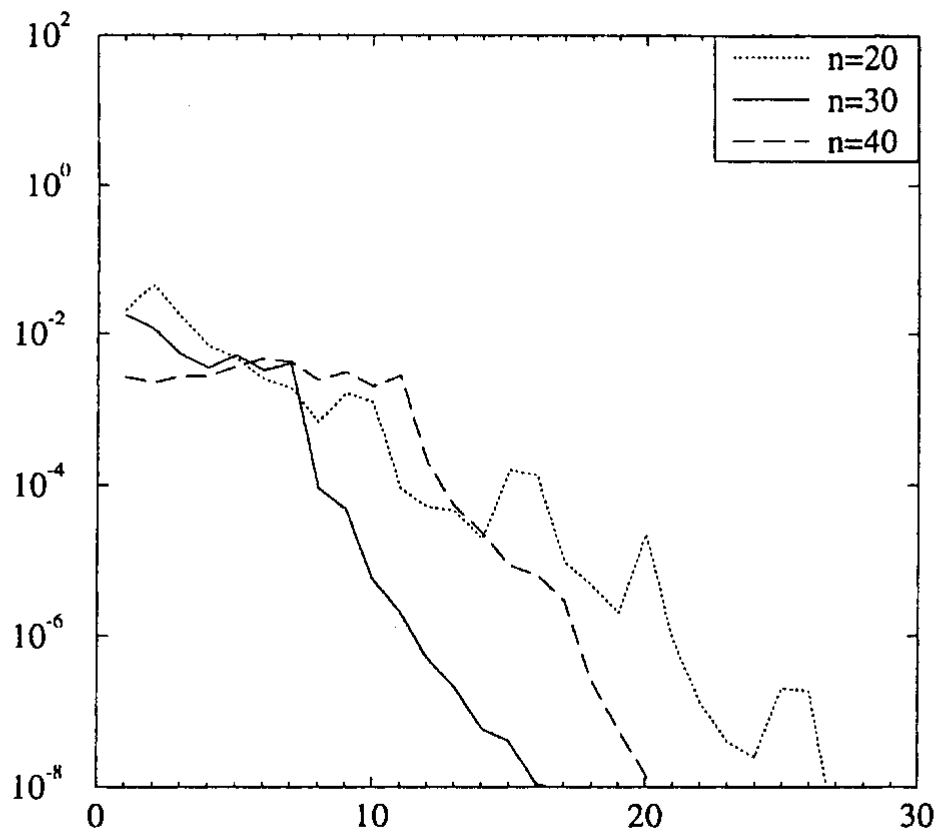
\includegraphics[width=.515\paperwidth]{images/fig-8-5-1.png}
  \caption{\(\varepsilon=10^{-2}\) 时 Galerkin 法在不同网格尺寸下的收敛过程}\label{fig:8.5.1}
\end{figure}
\begin{figure}[!htbp]
  \centering
  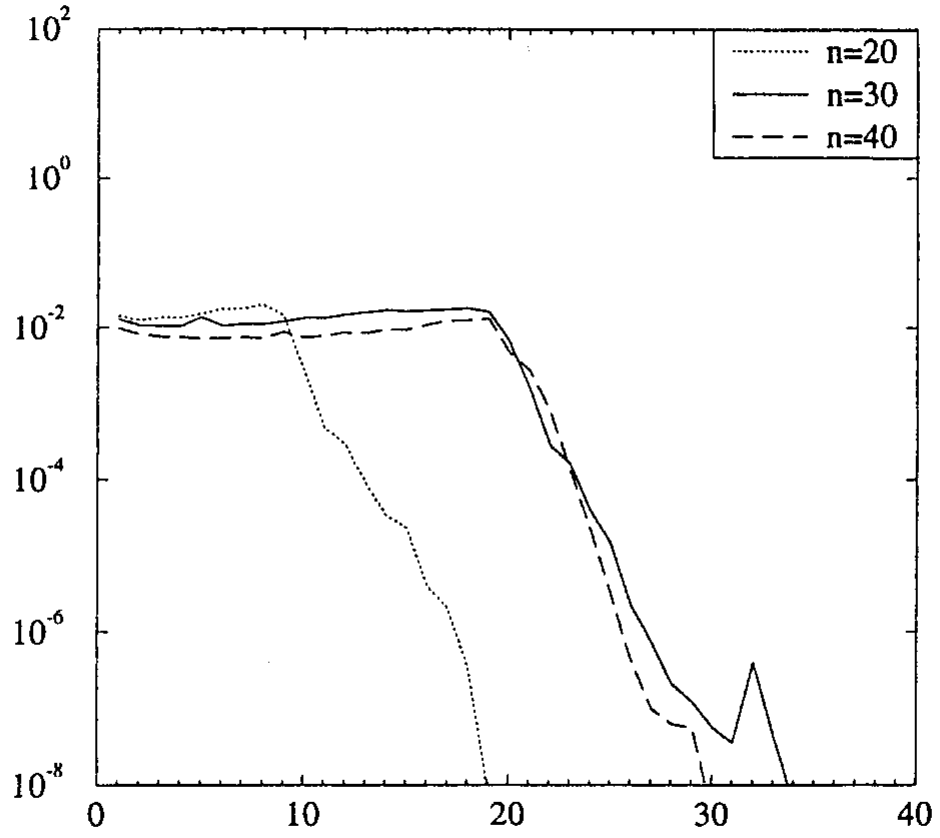
\includegraphics[width=.513\paperwidth]{images/fig-8-5-2.png}
  \caption{\(\varepsilon=10^{-2}\) 时 GALS 法在不同网格尺寸下的收敛过程}\label{fig:8.5.2}
\end{figure}
\begin{figure}[!htbp]
  \centering
  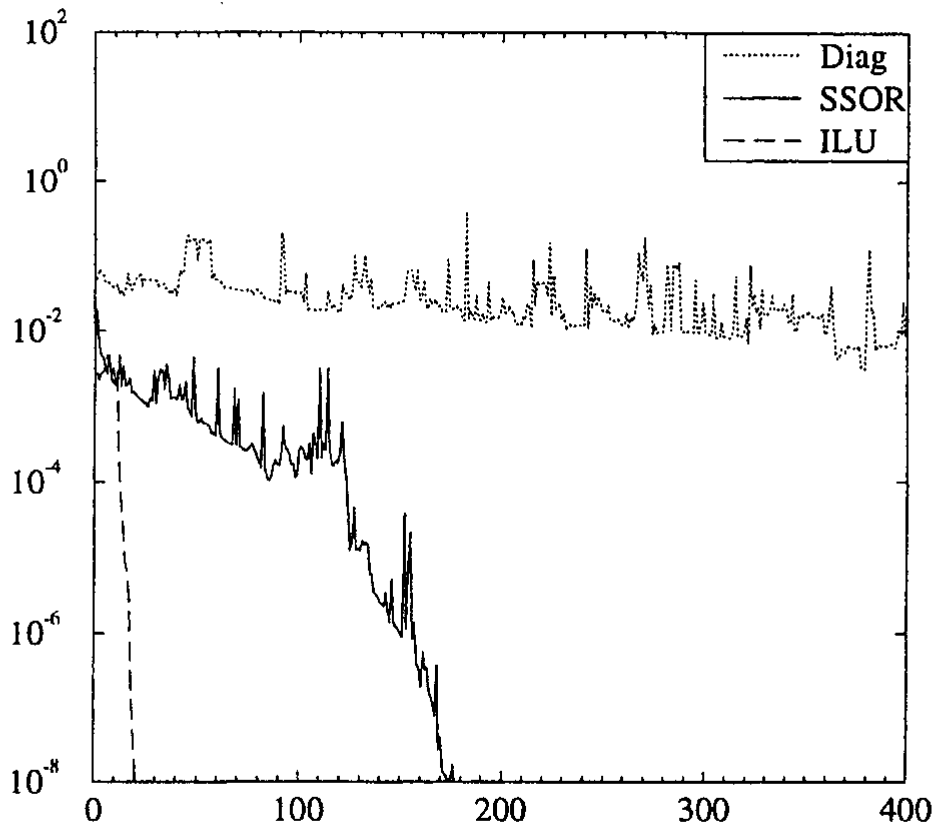
\includegraphics[width=.514\paperwidth]{images/fig-8-5-3.png}
  \caption{\(\varepsilon=10^{-3}\)、\(n=40\) 时 Galerkin 法使用不同预条件矩阵的收敛过程}\label{fig:8.5.3}
\end{figure}
\begin{figure}[!htbp]
  \centering
  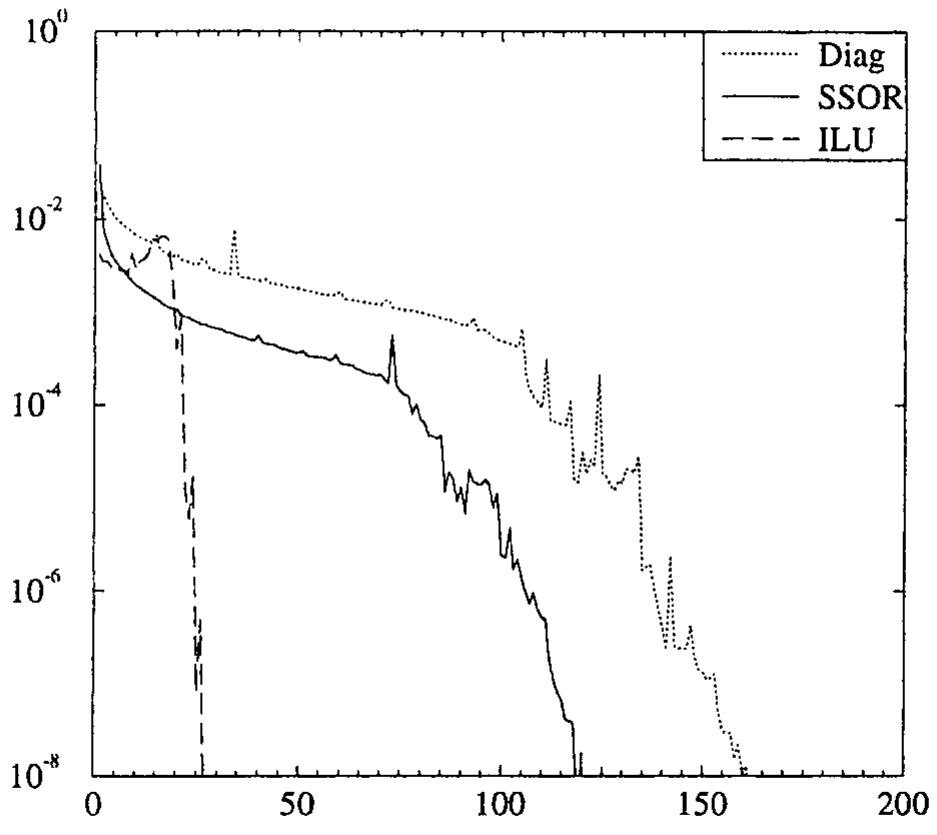
\includegraphics[width=.511\paperwidth]{images/fig-8-5-4.png}
  \caption{\(\varepsilon=10^{-3}\)、\(n=40\) 时 GALS 法使用不同预条件矩阵的收敛过程}\label{fig:8.5.4}
\end{figure}
\begin{figure}[!htbp]
  \centering
  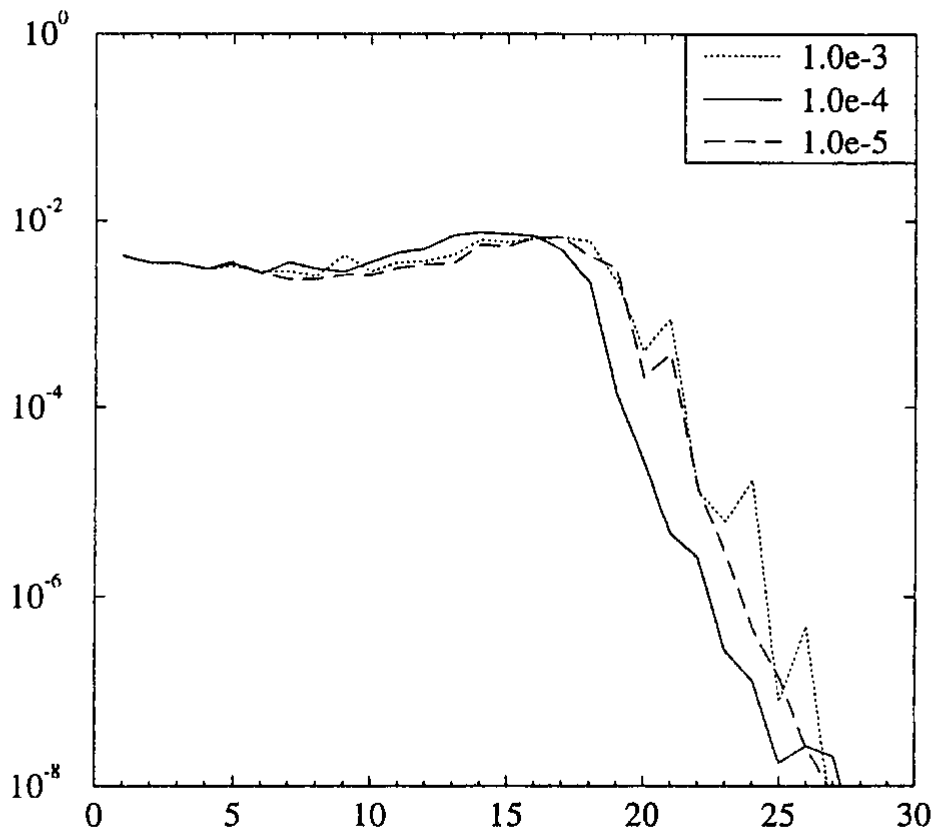
\includegraphics[width=.514\paperwidth]{images/fig-8-5-5.png}
  \caption{\(n=40\) 时 GALS 法对不同 \(\varepsilon\) 的收敛过程}\label{fig:8.5.5}
\end{figure}

\clearpage
\section{异质方法}\label{sec:8.6}
\SourcePage{299}

这里考察另一种方法,可用来逼近形如\eqref{eq:8.3.1}的对流占优的对流--扩散问题.

具体来说,假设\eqref{eq:8.3.1}对应的算子 \(L\) 由\eqref{eq:8.1.1}给出,将它改写为
\[
  Lz=L_1z+L_2z,
\]
其中
\begin{align}
  L_2z&:=-\sum_{i,j=1}^d D_i(a_{ij}D_jz),\label{eq:8.6.1}\\
  L_1z&:=\sum_{i=1}^d D_i(b_iz)+a_0z.\label{eq:8.6.2}
\end{align}
假设\eqref{eq:8.3.12}中定义的函数 \(\alpha_0(\boldsymbol{x})\) 满足
\begin{equation}\label{eq:8.6.3}
  0<\alpha_0\le\alpha_0(\boldsymbol{x})\le\alpha^*
      \qquad\text{在 }\Omega\text{ 上几乎处处},
\end{equation}
且\eqref{eq:6.1.20}成立,使得 \(L\) 对应的双线性形式 \(a(\cdot,\cdot)\) 在 \(H_0^1(\Omega)\) 上具有强制性.此外,假定常数 \(\alpha^*\) 与 \(\boldsymbol{b}\) 的大小相比很小,即
\SourcePage{300}
\[
  \widehat\alpha:=\frac{\alpha^*}{\|\boldsymbol{b}\|_{L^\infty(\Omega)}}\ll1.
\]
因此,可以预期出现边界层或内部层,宽度分别与 \(\widehat\alpha\) 或 \(\sqrt{\widehat\alpha}\) 成正比.

为明确起见,集中讨论边界层.若大致知道边界层的位置(实际中常常如此),就可以只在层的邻域内使用完整算子 \(L\),因为依赖于 \(\alpha_0(\boldsymbol{x})\) 的扩散项只有在那里才有显著影响.在其余区域,可以用\emph{简化算子} \(L_1\) 代替 \(L\),略去黏性的贡献.

\(L_1\) 是一个一阶双曲型算子,属于第~\BookRef{ch:14}{14}~章考察的算子族.这里只指出,在若干情形下,求解双曲型问题 \(L_1u=f\) 的计算量小于求解完整问题 \(Lu=f\) 的计算量.此外,在远离边界层的地方,双曲型问题通常可以用粗网格求解而不影响精度,从而只需在陡峭层附近使用细网格.

显然,这种方法要求将计算区域 \(\Omega\) 分为两个互不相交的区域 \(\Omega_1\) 和 \(\Omega_2\),使 \(\Omega_1\cap\Omega_2=\varnothing\) 且 \(\overline\Omega_1\cup\overline\Omega_2=\overline\Omega\).因此,需要在界面 \(\Gamma:=\partial\Omega_1\cap\partial\Omega_2\) 上对 \(\Omega_2\) 中完整问题的解和 \(\Omega_1\) 中简化问题的解施加适当的匹配条件.

\SourcePage{301}为简便起见,仅讨论齐次 Dirichlet 问题\eqref{eq:8.3.1}.\BookCite{gastaldi-quarteroni-sacchilandriani1990}{Gastaldi、Quarteroni 和 Sacchi Landriani(1990)}提出了下列\emph{耦合问题}：
\begin{equation}\label{eq:8.6.4}
  \begin{cases}
    Lu_2=f,&\text{在 }\Omega_2\text{ 内},\\
    L_1u_1=f,&\text{在 }\Omega_1\text{ 内},\\
    u_2=u_1,&\text{在 }\Gamma^{\mathrm{in}}\text{ 上},\\
    \dfrac{\partial u_2}{\partial n_L}=-\boldsymbol{b}\cdot\boldsymbol{n}\,u_1,
          &\text{在 }\Gamma\text{ 上},\\
    u_2=0,&\text{在 }\partial\Omega_2\cap\partial\Omega\text{ 上},\\
    u_1=0,&\text{在 }\partial\Omega_1^{\mathrm{in}}\cap\partial\Omega\text{ 上},
  \end{cases}
\end{equation}
其中 \(\boldsymbol{n}=\boldsymbol{n}(\boldsymbol{x})\) 是 \(\partial\Omega_1\) 上的单位外法向量,\(\partial u_2/\partial n_L\) 表示 \(u_2\) 关于 \(\boldsymbol{n}\) 的余法向导数,即
\[
  \frac{\partial u_2}{\partial n_L}
     :=\sum_{i,j=1}^d a_{ij}D_ju_2\,n_i-\boldsymbol{b}\cdot\boldsymbol{n}\,u_2.
\]
最后,
\[
  \partial\Omega_1^{\mathrm{in}}
    :=\{\boldsymbol{x}\in\partial\Omega_1\mid \boldsymbol{b}(\boldsymbol{x})\cdot\boldsymbol{n}(\boldsymbol{x})<0\}
\]
\SourcePage{302}是区域 \(\Omega_1\) 的流入边界,并且 \(\Gamma^{\mathrm{in}}:=\partial\Omega_1^{\mathrm{in}}\cap\Gamma\),见\figref{fig:8.6.1}.

匹配条件\eqref{eq:8.6.4}中的第三个条件要求解只在 \(\Gamma^{\mathrm{in}}\) 上连续,第四个条件则在整个界面 \(\Gamma\) 上保证通量平衡.

耦合问题\eqref{eq:8.6.4}可看作求解完整方程\eqref{eq:8.3.1}的一种区域分解表述(见笔记~\ref{note:6.4.1}).由于两侧使用不同的算子,这类方法称为\emph{异质区域分解法},例如见\BookCite{quarteroni-pasquarelli-valli1992}{Quarteroni、Pasquarelli 和 Valli(1992)}.

注意,\eqref{eq:8.6.4}中的界面条件是下面完全椭圆型问题的界面条件所趋向的极限：
\begin{equation}\label{eq:8.6.5}
  L_\varepsilon u_\varepsilon=f\qquad\text{在 }\Omega\text{ 内},
\end{equation}
其中 \(\varepsilon>0\),
\begin{equation}\label{eq:8.6.6}
  L_\varepsilon z:=-\sum_{i,j=1}^d D_i(a_{ij}^\varepsilon D_jz)
     +\sum_{i=1}^d D_i(b_iz)+a_0z,
\end{equation}
并且
\begin{equation}\label{eq:8.6.7}
  a_{ij}^\varepsilon(\boldsymbol{x}):=
  \begin{cases}
    a_{ij}(\boldsymbol{x}),&\boldsymbol{x}\in\Omega_2,\\
    \varepsilon\delta_{ij},&\boldsymbol{x}\in\Omega_1.
  \end{cases}
\end{equation}
事实上,这时 \(L_\varepsilon u_\varepsilon=f\) 在 \(\Omega\) 内的解 \(u_\varepsilon\) 在 \(\Gamma\) 上满足
\SourcePage{303}
\begin{figure}[!htbp]
  \centering
  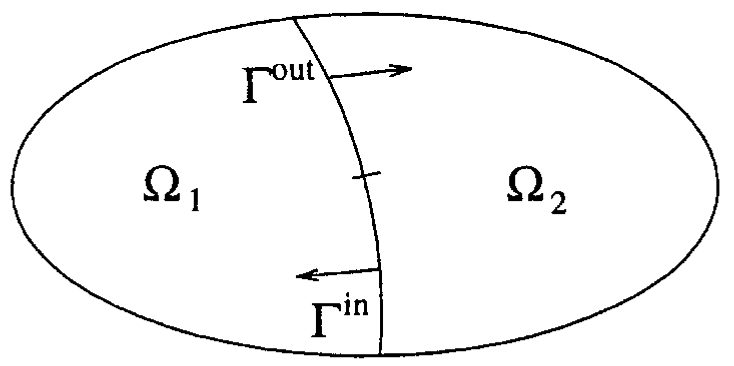
\includegraphics[width=.400\paperwidth]{images/fig-8-6-1.png}
  \caption{区域 \(\Omega\) 的分解}\label{fig:8.6.1}
\end{figure}
\begin{equation}\label{eq:8.6.8}
  \begin{cases}
    u_\varepsilon|_{\Omega_2}=u_\varepsilon|_{\Omega_1},\\
    \dfrac{\partial(u_\varepsilon|_{\Omega_2})}{\partial n_L}
       =\varepsilon\dfrac{\partial(u_\varepsilon|_{\Omega_1})}{\partial n}
         -\boldsymbol{b}\cdot\boldsymbol{n}\,u_\varepsilon|_{\Omega_1}.
  \end{cases}
\end{equation}
在取极限的过程中,解的连续性只在 \(\Gamma^{\mathrm{in}}\) 上保留.不过,可以证明,\(\Gamma\setminus\Gamma^{\mathrm{in}}\) 上的跳跃幅度与 \(\max_\Gamma\alpha_0(\boldsymbol{x})\) 一样小.

现在讨论\eqref{eq:8.6.4}的有限维逼近.先引入双线性形式
\begin{equation}\label{eq:8.6.9}
  a_2(z,v):=\int_{\Omega_2}
    \left[\sum_{i,j=1}^d a_{ij}D_jzD_iv-\sum_{i=1}^d b_izD_iv+a_0zv\right]
\end{equation}
\SourcePage{304}
及
\begin{equation}\label{eq:8.6.10}
  a_1(z,v):=\int_{\Omega_1}\left[-\sum_{i=1}^d b_izD_iv+a_0zv\right].
\end{equation}
于是,将\eqref{eq:8.6.4}改写为：求 \(u_2\in H^1_{\partial\Omega_2\setminus\Gamma}(\Omega_2)\)、\(u_1\in L^2(\Omega_1)\),使
\begin{equation}\label{eq:8.6.11}
  \left\{
  \begin{aligned}
    &a_2(u_2,v_2)-(\boldsymbol{b}\cdot\boldsymbol{n}\,u_2,v_2)_{\Gamma^{\mathrm{in}}}\\
    &\quad=(f,v_2)_{\Omega_2}+(\boldsymbol{b}\cdot\boldsymbol{n}\,u_1,v_2)_{\Gamma^{\mathrm{out}}}
         \qquad\forall\,v_2\in H^1_{\partial\Omega_2\setminus\Gamma}(\Omega_2),\\
    &a_1(u_1,v_1)+(\boldsymbol{b}\cdot\boldsymbol{n}\,u_1,v_1)_{\partial\Omega_1^{\mathrm{out}}}\\
    &\quad=(f,v_1)_{\Omega_1}-(\boldsymbol{b}\cdot\boldsymbol{n}\,u_2,v_1)_{\Gamma^{\mathrm{in}}}
          \qquad\forall\,v_1\in H^1(\Omega_1),
  \end{aligned}
  \right.
\end{equation}
其中 \(\Gamma^{\mathrm{out}}:=\Gamma\setminus\Gamma^{\mathrm{in}}\)、\(\partial\Omega_1^{\mathrm{out}}:=\partial\Omega_1\setminus\partial\Omega_1^{\mathrm{in}}\),并且
\[
  H^1_{\partial\Omega_2\setminus\Gamma}(\Omega_2)
      :=\{v\in H^1(\Omega_2)\mid v=0\text{ 在 }\partial\Omega_2\setminus\Gamma\text{ 上}\}
\]
(见第~\ref{sec:1.3}~节).在涉及 \(u_1\) 的边界项中,用 \(\boldsymbol{b}u_1\) 的法向迹解释其通量.

注意,\eqref{eq:8.6.11}的第一个方程保证\eqref{eq:8.6.4}中的第一个方程成立,此外还给出
\begin{align}
  \sum_{i,j=1}^d a_{ij}(D_ju_2)n_i&=0
    &&\text{在 }\Gamma^{\mathrm{in}}\text{ 上},\label{eq:8.6.12}\\
  \frac{\partial u_2}{\partial n_L}&=-\boldsymbol{b}\cdot\boldsymbol{n}\,u_1
    &&\text{在 }\Gamma^{\mathrm{out}}\text{ 上}.\label{eq:8.6.13}
\end{align}
而\eqref{eq:8.6.11}的第二个方程蕴含\eqref{eq:8.6.4}的第二个方程以及
\begin{equation}\label{eq:8.6.14}
  u_1=u_2\qquad\text{在 }\Gamma^{\mathrm{in}}\text{ 上}.
\end{equation}
界面条件\eqref{eq:8.6.12}至\eqref{eq:8.6.14}显然等价于\eqref{eq:8.6.4}的第三个和第四个条件.

还应注意,从\eqref{eq:8.6.11}的第二个方程可知,\(u_1\) 确实满足 \(\operatorname{div}(\boldsymbol{b}u_1)\in L^2(\Omega_1)\),所以 \(\partial\Omega_1\) 上的迹 \(\boldsymbol{b}\cdot\boldsymbol{n}\,u_1\) 有明确定义(见定理~\ref{thm:1.3.2}).

可以通过逐子域迭代有效地求解\eqref{eq:8.6.11},交替地在各自的区域内求解双曲型方程和椭圆型方程.这种策略便于数值计算,因为两个区域可以采用不同的求解器,甚至可以采用不同的空间离散.

下面给出\eqref{eq:8.6.11}基于 Galerkin 法的有限维逼近.设 \(V_{2,h}\) 和 \(V_{1,h}\) 分别为 \(H^1_{\partial\Omega_2\setminus\Gamma}(\Omega_2)\) 和 \(H^1(\Omega_1)\) 的适当有限维子空间.离散问题写成：求 \(u_{2,h}\in V_{2,h}\)、\(u_{1,h}\in V_{1,h}\),使
\SourcePage{305}
\begin{equation}\label{eq:8.6.15}
  \left\{
  \begin{aligned}
    &a_2(u_{2,h},v_{2,h})-(\boldsymbol{b}\cdot\boldsymbol{n}\,u_{2,h},v_{2,h})_{\Gamma^{\mathrm{in}}}\\
    &\quad=(f,v_{2,h})_{\Omega_2}+(\boldsymbol{b}\cdot\boldsymbol{n}\,u_{1,h},v_{2,h})_{\Gamma^{\mathrm{out}}}
         \qquad\forall\,v_{2,h}\in V_{2,h},\\
    &a_1(u_{1,h},v_{1,h})+(\boldsymbol{b}\cdot\boldsymbol{n}\,u_{1,h},v_{1,h})_{\partial\Omega_1^{\mathrm{out}}}\\
    &\quad=(f,v_{1,h})_{\Omega_1}-(\boldsymbol{b}\cdot\boldsymbol{n}\,u_{2,h},v_{1,h})_{\Gamma^{\mathrm{in}}}
         \qquad\forall\,v_{1,h}\in V_{1,h}.
  \end{aligned}
  \right.
\end{equation}
求解这一问题的一种有效迭代方法如下.给定任意初始近似 \(u_{2,h}^0\in V_{2,h}\),对 \(k\ge1\) 先求解
\begin{equation}\label{eq:8.6.16}
  \begin{aligned}
    &a_1(u_{1,h}^k,v_{1,h})+(\boldsymbol{b}\cdot\boldsymbol{n}\,u_{1,h}^k,v_{1,h})_{\partial\Omega_1^{\mathrm{out}}}\\
    &\quad=(f,v_{1,h})_{\Omega_1}-(\boldsymbol{b}\cdot\boldsymbol{n}\,u_{2,h}^{k-1},v_{1,h})_{\Gamma^{\mathrm{in}}}
         \qquad\forall\,v_{1,h}\in V_{1,h},
  \end{aligned}
\end{equation}
再求解
\begin{equation}\label{eq:8.6.17}
  \begin{aligned}
    &a_2(u_{2,h}^k,v_{2,h})-(\boldsymbol{b}\cdot\boldsymbol{n}\,u_{2,h}^k,v_{2,h})_{\Gamma^{\mathrm{in}}}\\
    &\quad=(f,v_{2,h})_{\Omega_2}+(\boldsymbol{b}\cdot\boldsymbol{n}\,u_{1,h}^k,v_{2,h})_{\Gamma^{\mathrm{out}}}
         \qquad\forall\,v_{2,h}\in V_{2,h}.
  \end{aligned}
\end{equation}
这两个问题都可求解,因为相应的矩阵正定.

\begin{figure}[!htbp]
  \centering
  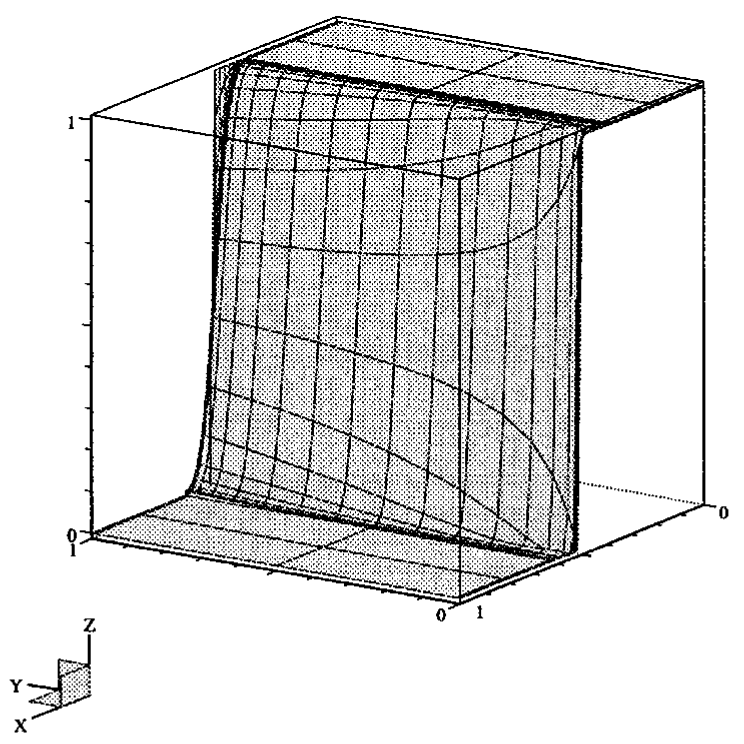
\includegraphics[width=.406\paperwidth]{images/fig-8-6-2.png}
  \caption{用异质方法为具有一个内部层的第一个测试问题计算的数值解}\label{fig:8.6.2}
\end{figure}

在二维情形,\BookCite{gastaldi-quarteroni-sacchilandriani1990}{Gastaldi、Quarteroni 和 Sacchi Landriani(1990)}证明了采用谱配置法时这一迭代格式的收敛性,且收敛速率与离散参数 \(h\) 无关.\SourcePage{306}也可使用加速参数 \(\theta_k>0\),将\eqref{eq:8.6.16}右端的 \(u_{2,h}^{k-1}\) 替换为 \(\lambda_h^{k-1}:=\theta_ku_{2,h}^{k-1}+(1-\theta_k)u_{1,h}^{k-1}\),这里还需要另选一个初值 \(u_{1,h}^0\in V_{1,h}\).

关于这一方法实际表现的全面介绍,见\BookCite{quarteroni-pasquarelli-valli1992}{Quarteroni、Pasquarelli 和 Valli(1992)}及\BookCite{frati-pasquarelli-quarteroni1993}{Frati、Pasquarelli 和 Quarteroni(1993)}.

\BookCite{brezzi-canuto-russo1989}{Brezzi、Canuto 和 Russo(1989)}提出了另一种处理椭圆型与双曲型耦合的方法,称为 \(\chi\) 表述,亦见\BookCite{canuto-russo1993}{Canuto 和 Russo(1993)}及其中所引文献.

下面给出两个用异质方法得到的数值结果,其中将 \(\Omega\subset\mathbb R^2\) 划分成两个以上的子区域.\figref{fig:8.6.2}是\figref{fig:8.3.3}\subref{fig:8.3.3a}的对应结果.将 \(\Omega\) 划分成九个子区域,只在含有内部层的三个子区域中求解完整的椭圆型问题(\(\varepsilon=10^{-3}\)),其余各子区域令 \(\varepsilon=0\).用 Legendre 谱配置法计算数值解,总共采用 874 个配置点.

\figref{fig:8.6.3}对应对流场 \(\boldsymbol{b}=(x_1,x_2)\)、\(\varepsilon=10^{-4}\) 的情形.将 \(\Omega\) 划分成九个子区域：一个较大的内部“双曲型”子区域和八个紧邻边界的狭长子区域.在后八个子区域中求解完整的椭圆型问题.“双曲型”子区域采用 9 个配置点,每个角部子区域采用 49 个,其余四个“边界”子区域各采用 21 个.

\begin{figure}[!htbp]
  \centering
  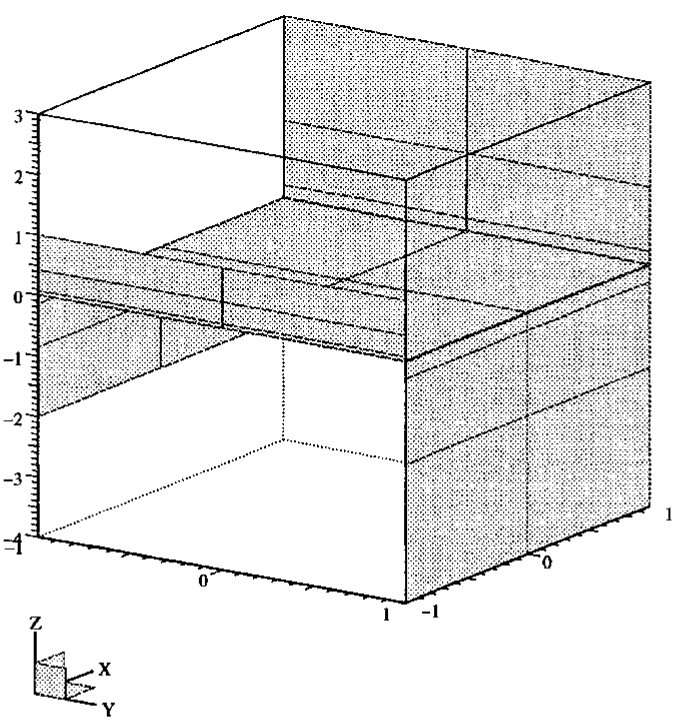
\includegraphics[width=.372\paperwidth]{images/fig-8-6-3.png}
  \caption{用异质方法为具有四个边界层的第二个测试问题计算的数值解}\label{fig:8.6.3}
\end{figure}

\chapter{Stokes 问题}\label{ch:9}
\SourcePage{307}

本章讨论 Stokes 微分方程组,可写成
\begin{equation}\tag{9.1}\label{eq:9.1}
  \begin{cases}
    a_0\boldsymbol{u}-\nu\Delta\boldsymbol{u}+\nabla p=\boldsymbol{f},
      &\text{在 }\Omega\subset\mathbb R^d\text{ 内},\quad d=2,3,\\
    \operatorname{div}\boldsymbol{u}=0,&\text{在 }\Omega\text{ 内},\\
    \boldsymbol{u}=0,&\text{在 }\partial\Omega\text{ 上},
  \end{cases}
\end{equation}
其中 \(a_0\ge0\) 和 \(\nu>0\) 是给定常数,\(\boldsymbol{f}\colon\Omega\to\mathbb R^d\) 是给定函数,\(\boldsymbol{u}\colon\Omega\to\mathbb R^d\) 和 \(p\colon\Omega\to\mathbb R\) 是待求的未知量.

在流体力学中求解局限于 \(\Omega\) 内的流动的 Navier--Stokes 方程时,\eqref{eq:9.1}可作为求解过程中的一环出现,例如用半隐式格式或分裂法推进时间时.在这些情形下,\(a_0\) 几乎总起时间步长倒数的作用.Navier--Stokes 方程的完整推导见第~\BookRef{sec:13.1}{13.1}~节.另一个例子是黏性很大、Reynolds 数很小的流体缓慢运动,此时 \(a_0=0\),而 \(\boldsymbol{f}\) 表示单位质量所受的外力.两种情形中,\(p\) 都表示流体压力与密度之比,\(\boldsymbol{u}\) 则表示速度.

\eqref{eq:9.1}采用经典的齐次 Dirichlet 边界条件.也可在 \(\partial\Omega\) 上施加涉及 \(\boldsymbol{u}\) 的法向导数,或该导数与 \(p\) 的线性组合的其他条件,这将在第~\BookRef{sec:10.1.1}{10.1.1}~节指出.

\section{数学表述与分析}\label{sec:9.1}

假定 \(\boldsymbol{f}\in(L^2(\Omega))^d\),并令
\(\mathcal V:=\{\boldsymbol{v}\in(\mathcal D(\Omega))^d\mid\operatorname{div}\boldsymbol{v}=0\}\)
及 \(V:=(H_0^1(\Omega))^d\),其中 \(V\) 为 Hilbert 空间.由\eqref{eq:9.1}的第一个方程以及 Green 公式\eqref{eq:5.1.2}和\eqref{eq:5.1.5},得到
\begin{equation}\label{eq:9.1.1}
  a_0(\boldsymbol{u},\boldsymbol{v})+\nu(\nabla\boldsymbol{u},\nabla\boldsymbol{v})
      -(p,\operatorname{div}\boldsymbol{v})=(\boldsymbol{f},\boldsymbol{v})
      \qquad\forall\,\boldsymbol{v}\in(\mathcal D(\Omega))^d,
\end{equation}
因而
\SourcePage{308}
\begin{equation}\label{eq:9.1.2}
  a_0(\boldsymbol{u},\boldsymbol{v})+\nu(\nabla\boldsymbol{u},\nabla\boldsymbol{v})
      =(\boldsymbol{f},\boldsymbol{v})\qquad\forall\,\boldsymbol{v}\in\mathcal V.
\end{equation}

\begin{definition*}
定义空间
\begin{equation}\label{eq:9.1.3}
  V_{\mathrm{div}}:=\{\boldsymbol{v}\in V\mid\operatorname{div}\boldsymbol{v}=0\}.
\end{equation}
\end{definition*}
这是 \(V\) 的闭子空间.由 Poincaré 不等式\eqref{eq:1.3.2}可知,它关于范数
\begin{equation}\label{eq:9.1.4}
  \|\boldsymbol{v}\|:=\|\nabla\boldsymbol{v}\|_0
\end{equation}
为 Hilbert 空间.由此可知,双线性形式
\begin{equation}\label{eq:9.1.5}
  a(\boldsymbol{w},\boldsymbol{v}):=a_0(\boldsymbol{w},\boldsymbol{v})
      +\nu(\nabla\boldsymbol{w},\nabla\boldsymbol{v}),\qquad \boldsymbol{w},\boldsymbol{v}\in V
\end{equation}
在 \(V_{\mathrm{div}}\times V_{\mathrm{div}}\) 上具有强制性.此外,映射 \(\boldsymbol{v}\mapsto(\boldsymbol{f},\boldsymbol{v})\) 在 \(V_{\mathrm{div}}\) 上线性且连续,所以由 Lax--Milgram 引理可知,问题
\begin{equation}\label{eq:9.1.6}
  \text{求 }\boldsymbol{u}\in V_{\mathrm{div}},\quad\text{使}\quad
     a(\boldsymbol{u},\boldsymbol{v})=(\boldsymbol{f},\boldsymbol{v})
      \qquad\forall\,\boldsymbol{v}\in V_{\mathrm{div}}
\end{equation}
有唯一解.

下面将用到下列结果.

\begin{lemma}[]{9.1.1}
设 \(\Omega\) 为 \(\mathbb R^d\) 中具有 Lipschitz 连续边界的有界区域,且 \(L\in V'\),即 \(L\) 是 \(V\) 上的连续线性泛函.则 \(L\) 在 \(V_{\mathrm{div}}\) 上恒为零,当且仅当存在 \(p\in L^2(\Omega)\),使
\begin{equation}\label{eq:9.1.7}
  L(\boldsymbol{v})=(p,\operatorname{div}\boldsymbol{v})\qquad\forall\,\boldsymbol{v}\in V.
\end{equation}
此外,\eqref{eq:9.1.7}确定的函数 \(p\) 在相差一个加性常数的意义下唯一.
\end{lemma}

为简便起见,这里省略这一引理的证明,例如可见\BookCite{girault-raviart1986}{Girault 和 Raviart(1986)}第 22 页.

现在可以证明下列定理.

\begin{theorem}[]{9.1.1}
设 \(\Omega\) 为 \(\mathbb R^d\) 中具有 Lipschitz 连续边界的有界区域.对于每个 \(\boldsymbol{f}\in(L^2(\Omega))^d\),令 \(\boldsymbol{u}\) 为\eqref{eq:9.1.6}的解.则存在 \(p\in L^2(\Omega)\),在相差一个加性常数的意义下唯一,使
\begin{equation}\label{eq:9.1.8}
  a(\boldsymbol{u},\boldsymbol{v})-(p,\operatorname{div}\boldsymbol{v})=(\boldsymbol{f},\boldsymbol{v})
      \qquad\forall\,\boldsymbol{v}\in V.
\end{equation}
\end{theorem}

\begin{proof}
令 \(\boldsymbol{u}\) 是\eqref{eq:9.1.6}的解,并定义
\[
  L(\boldsymbol{v}):=a(\boldsymbol{u},\boldsymbol{v})-(\boldsymbol{f},\boldsymbol{v})
      \qquad\forall\,\boldsymbol{v}\in V.
\]
\SourcePage{309}由\eqref{eq:9.1.6}可知,\(L\) 满足引理~\ref{lem:9.1.1}的假设.因此,存在 \(p\in L^2(\Omega)\),使 \((\boldsymbol{u},p)\) 是\eqref{eq:9.1.8}的解.\hfill\(\square\)
\end{proof}

现在给出另一种方法.定义 Hilbert 空间 \(Q=L_0^2(\Omega)\),其中
\begin{equation}\label{eq:9.1.9}
  L_0^2(\Omega):=\left\{q\in L^2(\Omega)\ \middle|\ \int_\Omega q=0\right\},
\end{equation}
并定义双线性形式
\begin{equation}\label{eq:9.1.10}
  b(\boldsymbol{v},q):=-(q,\operatorname{div}\boldsymbol{v}),\qquad
  \boldsymbol{v}\in V,\quad q\in Q.
\end{equation}
由定理~\ref{thm:9.1.1}可知,下列问题有唯一解：
\begin{equation}\label{eq:9.1.11}
  \left\{
  \begin{aligned}
    &\text{求 }\boldsymbol{u}\in V,\ p\in Q,\ \text{使}\\
    &a(\boldsymbol{u},\boldsymbol{v})+b(\boldsymbol{v},p)=(\boldsymbol{f},\boldsymbol{v})
       &&\forall\,\boldsymbol{v}\in V,\\
    &b(\boldsymbol{u},q)=0&&\forall\,q\in Q.
  \end{aligned}
  \right.
\end{equation}
这里用零平均值条件选定了原先只确定到一个加性常数的压力.

还需说明,\eqref{eq:9.1.11}的解也是\eqref{eq:9.1}的解.这可以用经典的稠密性论证.由于 \((\mathcal D(\Omega))^d\) 在 \(V\) 中稠密,即 \(V\) 是它关于 \((H^1(\Omega))^d\) 范数的闭包,可在\eqref{eq:9.1.11}中取任意 \(\boldsymbol{v}\in(\mathcal D(\Omega))^d\).分部积分可知,\eqref{eq:9.1}的第一个方程在分布意义下成立.事实上,因 \(\boldsymbol{f}\in(L^2(\Omega))^d\),该方程的左端作为一个整体可由 \(L^2\) 函数表示,等式几乎处处成立.最后,\eqref{eq:9.1.11}的最后一个方程保证 \(\operatorname{div}\boldsymbol{u}=0\) 几乎处处成立,因为 \(\operatorname{div}\boldsymbol{u}\in Q\) 且与 \(Q\) 中所有函数正交.

以下将\eqref{eq:9.1.11}称为 Stokes 方程的\emph{弱形式}.

\begin{note}\NumberedNote{note:9.1.1}{\heiti(压力空间的另一种选择)}
由\eqref{eq:9.1}及前面的分析可知,压力 \(p\) 是 \(L^2(\Omega)\) 中只确定到一个加性常数的函数.消除这种不确定性的一种方法是寻找在 \(\Omega\) 上平均值为零的压力,即取 \(p\) 属于\eqref{eq:9.1.9}定义的空间 \(L_0^2(\Omega)\).这一选择很合适,尤其是用谱方法逼近\eqref{eq:9.1.11}时.事实上,为求得平均值为零的离散压力,只需去掉它的最低次 Fourier 系数,即与常数多项式对应的那个系数(见第~\ref{ch:4}~章).

不过,对有限元或有限差分等局部型有限维逼近而言,平均值的整体约束可能不便处理.这时,可用商空间 \(L^2(\Omega)/\mathbb R\) 代替压力空间 \(Q\).这样,在离散层次上,例如可\SourcePage{310}预先指定压力在区域 \(\Omega\) 内某个给定点处的值.\hfill\(\square\)
\end{note}

\begin{note}\NumberedNote{note:9.1.2}{\heiti(鞍点表述)}
考察 Lagrange 泛函
\begin{equation}\label{eq:9.1.12}
  \mathcal L(\boldsymbol{v},q):=\tfrac12a(\boldsymbol{v},\boldsymbol{v})+b(\boldsymbol{v},q)
       -(\boldsymbol{f},\boldsymbol{v}),\qquad \boldsymbol{v}\in V,\quad q\in Q.
\end{equation}
Stokes 问题\eqref{eq:9.1.11}的解 \((\boldsymbol{u},p)\) 是上述泛函的一个鞍点,即
\begin{equation}\label{eq:9.1.13}
  \mathcal L(\boldsymbol{u},p)=\min_{\boldsymbol{v}\in V}\max_{q\in Q}\mathcal L(\boldsymbol{v},q).
\end{equation}
反过来也成立.证明例如可见\BookCite{temam1984}{Temam(1984)}、\BookCite{glowinski-letallec1989}{Glowinski 和 Le Tallec(1989)},另见第~\ref{sec:7.1.2}~节.从这个角度看,\(p\) 是无散度约束对应的 Lagrange 乘子.\hfill\(\square\)
\end{note}

\section{Galerkin 逼近}\label{sec:9.2}

上一节的分析给出了 Stokes 问题\eqref{eq:9.1}的两种弱形式.第一种由\eqref{eq:9.1.6}给出,求解它便得到速度场 \(\boldsymbol{u}\).在速度已知后,可以通过\eqref{eq:9.1.8}或其他适用的方法恢复压力 \(p\).另一种弱形式是\eqref{eq:9.1.11},它又与鞍点问题\eqref{eq:9.1.13}等价.

这两种表述提示了数值求解 Stokes 问题的两条途径.先从较易分析的\eqref{eq:9.1.6}入手,不过后面将主要讨论\eqref{eq:9.1.11}的数值逼近.按照第~\ref{sec:5.2}~节的方法,\eqref{eq:9.1.6}的 Galerkin 逼近为
\begin{equation}\label{eq:9.2.1}
  \text{求 }\boldsymbol{u}_h\in V_{\mathrm{div},h},\quad\text{使}\quad
    a(\boldsymbol{u}_h,\boldsymbol{v}_h)=(\boldsymbol{f},\boldsymbol{v}_h)
       \qquad\forall\,\boldsymbol{v}_h\in V_{\mathrm{div},h},
\end{equation}
其中 \(\{V_{\mathrm{div},h}\}\) 是 \(V_{\mathrm{div}}\) 的一族有限维子空间,满足相容性假设
\begin{equation}\label{eq:9.2.2}
  \forall\,\boldsymbol{v}\in V_{\mathrm{div}},\qquad
     \inf_{\boldsymbol{v}_h\in V_{\mathrm{div},h}}\|\boldsymbol{v}-\boldsymbol{v}_h\|\to0
       \quad\text{当 }h\to0.
\end{equation}
直接应用定理~\ref{thm:5.2.1}可知,\eqref{eq:9.2.1}存在唯一解.该解稳定,并收敛到\eqref{eq:9.1.6}的解 \(\boldsymbol{u}\).更确切地说,存在与 \(h\) 无关的常数 \(C\),使
\SourcePage{311}
\begin{equation}\label{eq:9.2.3}
  \|\boldsymbol{u}-\boldsymbol{u}_h\|\le C\inf_{\boldsymbol{v}_h\in V_{\mathrm{div},h}}
           \|\boldsymbol{u}-\boldsymbol{v}_h\|.
\end{equation}

这一结果在数学上很简洁,但实践中很少用\eqref{eq:9.2.1}逼近速度场.原因有两个.首先,很难找到空间\eqref{eq:9.1.3}的内逼近 \(V_{\mathrm{div},h}\),即一个由无散度向量值函数组成、又足够丰富的有限维空间,使\eqref{eq:9.2.3}给出随 \(h\) 变化的良好收敛性.其次,即使解决了这个问题,实际构造 \(V_{\mathrm{div},h}\) 的基也可能十分困难.文献中已有一些成功的例子,尤其是在谱逼近方面,例如见\BookCite{moser-moin-leonard1983}{Moser、Moin 和 Leonard(1983)}.采用有限元法时,可考虑调整\eqref{eq:9.2.1}中的有限维空间,见笔记~\BookRef{note:9.2.1}{9.2.1}.

现在转向\eqref{eq:9.1.11}.这个问题的形式并不陌生,第~\ref{ch:7}~章已经遇到过.按照第~\ref{sec:7.4}~节的方法,引入分别依赖于 \(h\) 的两族有限维子空间 \(V_h\subset V\) 和 \(Q_h\subset Q\),用下列离散问题逼近\eqref{eq:9.1.11}：
\begin{equation}\label{eq:9.2.4}
  \left\{
  \begin{aligned}
    &\text{求 }\boldsymbol{u}_h\in V_h,\ p_h\in Q_h,\ \text{使}\\
    &a(\boldsymbol{u}_h,\boldsymbol{v}_h)+b(\boldsymbol{v}_h,p_h)=(\boldsymbol{f},\boldsymbol{v}_h)
        &&\forall\,\boldsymbol{v}_h\in V_h,\\
    &b(\boldsymbol{u}_h,q_h)=0&&\forall\,q_h\in Q_h.
  \end{aligned}
  \right.
\end{equation}
为分析这个问题,令
\begin{equation}\label{eq:9.2.5}
  Z_h:=\{\boldsymbol{v}_h\in V_h\mid (q_h,\operatorname{div}\boldsymbol{v}_h)=0
      \quad\forall\,q_h\in Q_h\}.
\end{equation}
这是与这些有限维空间对应的离散无散度函数空间.由于 \(a(\cdot,\cdot)\) 在 \(V\) 上具有强制性,而 \(Z_h\) 是 \(V\) 的子空间,所以 \(a(\cdot,\cdot)\) 在 \(Z_h\) 上也具有强制性.也就是说,存在 \(\alpha>0\),使
\begin{equation}\label{eq:9.2.6}
  a_0\|\boldsymbol{v}_h\|_0^2+\nu\|\nabla\boldsymbol{v}_h\|_0^2\ge\alpha\|\boldsymbol{v}_h\|^2
    \qquad\forall\,\boldsymbol{v}_h\in Z_h.
\end{equation}
此外,仍用 Poincaré 不等式\eqref{eq:1.3.2},可知存在 \(\gamma>0\) 和 \(\delta>0\),使
\begin{equation}\label{eq:9.2.7}
  |a_0(\boldsymbol{w},\boldsymbol{v})+\nu(\nabla\boldsymbol{w},\nabla\boldsymbol{v})|
      \le\gamma\|\boldsymbol{w}\|\|\boldsymbol{v}\|\qquad\forall\,\boldsymbol{w},\boldsymbol{v}\in V,
\end{equation}
这表示双线性形式 \(a(\cdot,\cdot)\) 在 \(V\times V\) 上连续；并且
\begin{equation}\label{eq:9.2.8}
  |(q,\operatorname{div}\boldsymbol{v})|\le\delta\|\boldsymbol{v}\|\|q\|_0
      \qquad\forall\,\boldsymbol{v}\in V,\ q\in Q,
\end{equation}
这表示双线性形式 \(b(\cdot,\cdot)\) 在 \(V\times Q\) 上连续.

此外,假定空间 \(V_h\) 和 \(Q_h\) 具有下列性质：存在 \(\beta>0\),使
\SourcePage{312}
\begin{equation}\label{eq:9.2.9}
  \forall\,q_h\in Q_h,\ \exists\,\boldsymbol{v}_h\in V_h,\ \boldsymbol{v}_h\ne0:\qquad
      (q_h,\operatorname{div}\boldsymbol{v}_h)\ge\beta\|\boldsymbol{v}_h\|\|q_h\|_0.
\end{equation}
这称为\emph{相容性条件},也称为 \emph{inf--sup 条件}或 \emph{Ladyzhenskaya--Babuška--Brezzi 条件}.

在上述假设下,由定理~\ref{thm:7.4.2}可知,\eqref{eq:9.2.4}存在唯一解,并且该解满足
\begin{equation}\label{eq:9.2.10}
  \|\boldsymbol{u}_h\|\le\frac1\alpha\|\boldsymbol{f}\|_{V'},\qquad
  \|p_h\|_0\le\frac1\beta\left(1+\frac{\gamma}{\alpha}\right)\|\boldsymbol{f}\|_{V'}.
\end{equation}
这些估计表明,若 \(\beta\) 与 \(h\) 无关,则解稳定.若这一条件不成立,或更糟的是\eqref{eq:9.2.9}不成立,就称逼近\eqref{eq:9.2.4}不稳定.

定理~\ref{thm:7.4.3}给出的抽象收敛结论在这里化为
\begin{equation}\label{eq:9.2.11}
  \|\boldsymbol{u}-\boldsymbol{u}_h\|\le\left(1+\frac{\gamma}{\alpha}\right)
       \inf_{\boldsymbol{v}_h\in Z_h}\|\boldsymbol{u}-\boldsymbol{v}_h\|
       +\frac{\delta}{\alpha}\inf_{q_h\in Q_h}\|p-q_h\|_0
\end{equation}
和
\begin{equation}\label{eq:9.2.12}
  \begin{aligned}
    \|p-p_h\|_0&\le\frac{\gamma}{\beta}\left(1+\frac{\gamma}{\alpha}\right)
        \inf_{\boldsymbol{v}_h\in Z_h}\|\boldsymbol{u}-\boldsymbol{v}_h\|\\
       &\quad+\left(1+\frac{\delta}{\beta}+\frac{\gamma\delta}{\alpha\beta}\right)
         \inf_{q_h\in Q_h}\|p-q_h\|_0.
  \end{aligned}
\end{equation}
由\eqref{eq:7.4.26}可知
\[
  \inf_{\boldsymbol{v}_h\in Z_h}\|\boldsymbol{u}-\boldsymbol{v}_h\|
   \le\left(1+\frac{\delta}{\beta}\right)
         \inf_{\boldsymbol{v}_h\in V_h}\|\boldsymbol{u}-\boldsymbol{v}_h\|.
\]
所以,只要 \(\beta\) 与 \(h\) 无关,收敛估计就是最优的.

\begin{note}\NumberedNote{note:9.2.1}{\heiti(非协调逼近)}
为避免构造 \(V_{\mathrm{div},h}\) 的困难,可以将\eqref{eq:9.2.1}换成
\begin{equation}\label{eq:9.2.13}
  \text{求 }\boldsymbol{u}_h\in Z_h,\quad\text{使}\quad
  a(\boldsymbol{u}_h,\boldsymbol{v}_h)=(\boldsymbol{f},\boldsymbol{v}_h)\qquad\forall\,\boldsymbol{v}_h\in Z_h
\end{equation}
(见\eqref{eq:9.2.5}).一般来说,\(Z_h\) 不是 \(V_{\mathrm{div}}\) 的子空间,因为 \(Z_h\) 的元素未必无散度.因此,\eqref{eq:9.2.13}给出\eqref{eq:9.1.6}的一个{\heiti 非协调逼近}.

采用非协调有限维空间 \(Z_h\) 的主要好处是,构造一组基可能比较容易.例子见\BookCite{hecht1981}{Hecht(1981)}.如笔记~\ref{note:5.5.1}所示,在该笔记所述的其余条件下,若以 \(Z_h\) 代替 \(V_{\mathrm{div},h}\) 后相容性\eqref{eq:9.2.2}仍成立,就可以证明收敛性.\hfill\(\square\)
\end{note}

\subsection{Stokes 问题的代数形式}\label{sec:9.2.1}
\SourcePage{313}

先看问题\eqref{eq:9.2.1}.对任一固定的 \(h\),记 \(N_h^0\) 为子空间 \(V_{\mathrm{div},h}\) 的维数,并设 \(\{\boldsymbol{\varphi}_j^0\mid j=1,\ldots,N_h^0\}\) 是 \(V_{\mathrm{div},h}\) 的一组基.令
\[
  \boldsymbol{u}_h(\boldsymbol{x})=\sum_{j=1}^{N_h^0}\xi_j\boldsymbol{\varphi}_j^0(\boldsymbol{x}).
\]
则\eqref{eq:9.2.1}对应的线性方程组为
\[
  A^0\boldsymbol{\xi}=\boldsymbol{f},\qquad
     f_i:=(\boldsymbol{f},\boldsymbol{\varphi}_i^0),\quad
     A_{ij}^0:=a(\boldsymbol{\varphi}_j^0,\boldsymbol{\varphi}_i^0).
\]
矩阵 \(A^0\) 对称正定.

问题\eqref{eq:9.2.4}的情形较为复杂.现在分别以 \(N_h\) 和 \(K_h\) 记 \(V_h\) 和 \(Q_h\) 的维数,以 \(\{\boldsymbol{\varphi}_j\mid j=1,\ldots,N_h\}\) 和 \(\{\psi_l\mid l=1,\ldots,K_h\}\) 分别记 \(V_h\) 和 \(Q_h\) 的基.若令
\[
  \boldsymbol{u}_h(\boldsymbol{x})=\sum_{j=1}^{N_h}u_j\boldsymbol{\varphi}_j(\boldsymbol{x}),\qquad
  p_h(\boldsymbol{x})=\sum_{l=1}^{K_h}p_l\psi_l(\boldsymbol{x}),
\]
则\eqref{eq:9.2.4}对应的线性方程组具有如下形式：
\begin{equation}\label{eq:9.2.14}
  \begin{pmatrix}A&B^T\\B&0\end{pmatrix}
    \begin{pmatrix}\boldsymbol{u}\\\boldsymbol{p}\end{pmatrix}
       =\begin{pmatrix}\boldsymbol{f}\\0\end{pmatrix},
\end{equation}
其中
\begin{equation}\label{eq:9.2.15}
  A_{ij}:=a(\boldsymbol{\varphi}_j,\boldsymbol{\varphi}_i),\qquad
  B_{li}:=b(\boldsymbol{\varphi}_i,\psi_l),\qquad f_i:=(\boldsymbol{f},\boldsymbol{\varphi}_i).
\end{equation}
\(A\) 是 \(N_h\times N_h\) 的对称正定矩阵,而 \(B\) 是 \(K_h\times N_h\) 的矩形矩阵.用代数论证容易看出,相容性条件\eqref{eq:9.2.9}成立,当且仅当 \(\ker B^T=\{0\}\).此时,阶数为 \(N_h+K_h\) 的整体矩阵
\begin{equation}\label{eq:9.2.16}
  S:=\begin{pmatrix}A&B^T\\B&0\end{pmatrix}
\end{equation}
非奇异.事实上,这时由\eqref{eq:9.2.14}可得
\begin{align}
  \boldsymbol{u}&=A^{-1}(\boldsymbol{f}-B^T\boldsymbol{p}),\label{eq:9.2.17}\\
  BA^{-1}B^T\boldsymbol{p}&=BA^{-1}\boldsymbol{f}.\label{eq:9.2.18}
\end{align}
由于 \(K_h\times K_h\) 的对称\emph{压力矩阵}
\begin{equation}\label{eq:9.2.19}
  R:=BA^{-1}B^T
\end{equation}
在 \(\ker B^T=\{0\}\) 时正定,\(\boldsymbol{p}\) 和随后的 \(\boldsymbol{u}\) 可分别由\eqref{eq:9.2.18}和\eqref{eq:9.2.17}唯一确定.由此可知,\(S\) 非奇异.

\SourcePage{314}还应注意,\(S\) 对称但不定,所以它的特征值为实数,既有正值也有负值.

也可将\eqref{eq:9.2.14}换成等价的方程组,即把最后 \(K_h\) 行反号,用
\begin{equation}\label{eq:9.2.20}
  S':=\begin{pmatrix}A&B^T\\-B&0\end{pmatrix}
\end{equation}
代替 \(S\).这一矩阵不再对称.由于 \(A\) 正定,且在 \(\ker B^T=\{0\}\) 时,\(S'\) 的特征向量不可能只有压力分量,所以 \(S'\) 的所有特征值都有正实部.

若以 \(\sqrt{a(\boldsymbol{v},\boldsymbol{v})}\) 作为速度空间的等价范数,则\eqref{eq:9.2.8}和\eqref{eq:9.2.9}中的相应常数 \(\delta\) 和 \(\beta\) 与广义特征值问题
\[
  BA^{-1}B^T\boldsymbol{\omega}^k=\lambda_k J\boldsymbol{\omega}^k
\]
有关,其中 \(J_{lm}:=(\psi_l,\psi_m)\) 是压力质量矩阵.确切地说(例如,见\BookCite{fortin1993}{Fortin(1993)}),最优的 \(\beta\) 及任一连续性常数 \(\delta\) 满足
\[
  \beta=\sqrt{\lambda_{\min}},\qquad \delta\ge\sqrt{\lambda_{\max}}.
\]

\subsection{相容性条件与伪压力模态}\label{sec:9.2.2}

上一小节已表明,相容性条件\eqref{eq:9.2.9}保证 \(\ker B^T=\{0\}\),从而整体矩阵 \(S\) 非奇异.条件\eqref{eq:9.2.9}意味着,与离散压力空间 \(Q_h\) 相比,离散速度空间 \(V_h\) 足够丰富.

\eqref{eq:9.2.9}的另一个重要结果是排除了伪压力模态.
\begin{definition*}
伪模态是满足下列条件的任意函数 \(p_h^*\)：
\begin{equation}\label{eq:9.2.21}
  p_h^*\in Q_h,\qquad (p_h^*,\operatorname{div}\boldsymbol{v}_h)=0
      \qquad\forall\,\boldsymbol{v}_h\in V_h.
\end{equation}
\end{definition*}
任何这样的函数都使得对所有 \(\boldsymbol{v}_h\in V_h\) 和 \(c\in\mathbb R\),有
\(b(\boldsymbol{v}_h,p_h+cp_h^*)=b(\boldsymbol{v}_h,p_h)\).因此,\eqref{eq:9.2.4}确定的压力可以相差一个由伪模态线性组合而成的函数.这很容易导致压力计算不稳定.

现在可以看出,若相容性条件\eqref{eq:9.2.9}成立,则唯一可能的伪模态是平凡的 \(p_h^*=0\).事实上,若 \(p_h^*\) 是 \(Q_h\) 中任一非零函数,则\eqref{eq:9.2.9}保证存在 \(\boldsymbol{v}_h\in V_h\),使 \((p_h^*,\operatorname{div}\boldsymbol{v}_h)>0\).

于是有一个重要的问题：若有限维空间不满足相容性条件,数值格式会怎样？由前面的分析可知,\eqref{eq:9.2.11}和\eqref{eq:9.2.10}的第一个不等式都不依赖于常数 \(\beta\),因此只要逼近误差趋于零,速度场仍可稳定、收敛地得到.伪模态本身只会影响压力场.若还需要良好的离散压力 \(p_h\),显然可\SourcePage{315}选取满足\eqref{eq:9.2.9}的 \(Q_h\) 和 \(V_h\).若这一条件不满足,则可以采取几种补救措施.

一种典型的做法是对有限维方程组\eqref{eq:9.2.4}作\emph{稳定化},即放宽 \(\boldsymbol{u}_h\) 的不可压缩性约束.可以用多种方法来实现,严谨的数学分析能说明这些方法的依据.第~\BookRef{sec:9.4}{9.4}~节将讨论这一问题.

另一种做法是从算出的压力中\emph{滤除}伪模态.通常在迭代过程中每做完一步便进行滤除,这要求预先知道伪模态向量空间的结构.参见第~\BookRef{sec:9.5}{9.5}~节.

最后,在特定的逼近框架下,还有其他可行的方法.例如,有限元逼近可以采用\emph{宏单元},第~\BookRef{sec:9.3}{9.3}~节将说明这种技术.

\subsection{无散度性质与锁定现象}\label{sec:9.2.3}

一般来说,离散连续性条件
\begin{equation}\label{eq:9.2.22}
  b(\boldsymbol{u}_h,q_h)=0\qquad\forall\,q_h\in Q_h
\end{equation}
未必意味着
\begin{equation}\label{eq:9.2.23}
  \operatorname{div}\boldsymbol{u}_h=0.
\end{equation}
事实上,\eqref{eq:9.2.22}只蕴含 \(\boldsymbol{u}_h\in Z_h\)(见\eqref{eq:9.2.5}).如笔记~\ref{note:9.2.1}指出的,仅凭这一点无法得出\eqref{eq:9.2.23}.不过,若
\begin{equation}\label{eq:9.2.24}
  \operatorname{div}V_h\subset Q_h,
\end{equation}
则\eqref{eq:9.2.23}成立.事实上,只需在\eqref{eq:9.2.22}中取 \(q_h=\operatorname{div}\boldsymbol{u}_h\),即可得出\eqref{eq:9.2.23}.在 Stokes 问题的有限元逼近中,\eqref{eq:9.2.24}很少得到满足.

\(Q_h\) 越丰富,\eqref{eq:9.2.24}就越有可能成立.不过,这样做可能妨碍满足相容性条件\eqref{eq:9.2.9}.一个极端情形是 \(Q_h\) 相对于 \(V_h\) 过大,以至于\eqref{eq:9.2.22}对 \(\boldsymbol{u}_h\) 施加过强的约束,使它在满足\eqref{eq:9.2.23}的同时甚至有
\[
  \boldsymbol{u}_h=0.
\]
这种特有的行为称为速度场的\emph{锁定现象}.第~\BookRef{sec:9.3.1}{9.3.1}~节将给出一个例子.

\section{有限元逼近}\label{sec:9.3}
\SourcePage{316}

沿用第~\ref{ch:3}~章的记号.特别地,只考察多边形区域 \(\Omega\),以 \(\mathcal T_h\) 记 \(\overline\Omega\) 的一个剖分.剖分由直径不超过 \(h\) 的多面体 \(K\) 组成,简称单元.

若每个 \(K\) 为三角形或四面体,定义
\begin{equation}\label{eq:9.3.1}
  Y_h^k:=\{\varphi_h\in L^2(\Omega)\mid
    \varphi_h|_K\in\mathbb P_k\quad\forall\,K\in\mathcal T_h\},\qquad k\ge0.
\end{equation}
若每个 \(K\) 为平行四边形或平行六面体,则定义
\begin{equation}\label{eq:9.3.2}
  Y_h^k:=\{\varphi_h\in L^2(\Omega)\mid
    (\varphi_h|_K)\circ T_K\in\mathbb Q_k\quad\forall\,K\in\mathcal T_h\},\qquad k\ge0.
\end{equation}
也可以考察一般的四边形或六面体.不过,与第~\ref{ch:3}~章一样,这里只考虑最简单的情形.两种情形都令
\begin{equation}\label{eq:9.3.3}
  X_h^k=Y_h^k\cap C^0(\overline\Omega),\qquad k\ge1,
\end{equation}
与\eqref{eq:3.2.4}和\eqref{eq:3.2.5}一致.

显然,\(Y_h^m\cap L_0^2(\Omega)\)(\(m\ge0\))或 \(X_h^m\cap L_0^2(\Omega)\)(\(m\ge1\))是压力空间 \(Q_h\) 的合适候选空间,而 \(V_h\) 可取 \((X_h^k\cap H_0^1(\Omega))^d\),其中 \(k\ge1\).

下面给出这些空间的几种组合,逐一说明参考单元上每个速度分量及压力的自由度.

对于速度空间,需要将边界上的自由度固定为零,以使 \(\boldsymbol{u}_h\) 满足齐次 Dirichlet 条件.对于压力,若要求函数的平均值为零,或者要求它在 \(\overline\Omega\) 的某个给定点 \(\boldsymbol{x}^*\) 处为零,整体自由度总数都将减少一个.若采用后一种做法,选取间断空间 \(Y_h^m\) 有一个好处：在每个单元 \(K\) 上,除包含 \(\boldsymbol{x}^*\) 的单元 \(K^*\) 外,\(\boldsymbol{u}_h\) 的散度的平均值为零,即该单元内质量守恒.这一性质直接由\eqref{eq:9.2.4}的第二个方程得到,因为这时 \(Q_h\) 包含所有在 \(\overline\Omega\setminus K^*\) 上分片为常数且在 \(K^*\) 上为零的函数.

\subsection{压力间断的有限元}\label{sec:9.3.1}

本小节只考察二维情形.首先考虑
\begin{equation}\label{eq:9.3.4}
  Q_h=Y_h^m\cap L_0^2(\Omega),\quad m\ge0,\qquad
  V_h=(X_h^k\cap H_0^1(\Omega))^2,\quad k\ge1.
\end{equation}

\SourcePage{317}最简单的是 \(m=0\)、\(k=1\) 的情形,即压力分片常值,速度分片线性或双线性.自由度如\figref{fig:9.3.1}所示.符号 \(\bullet\) 表示速度分量的值,\(\square\) 表示压力值.

\begin{figure}[!htbp]
  \centering
  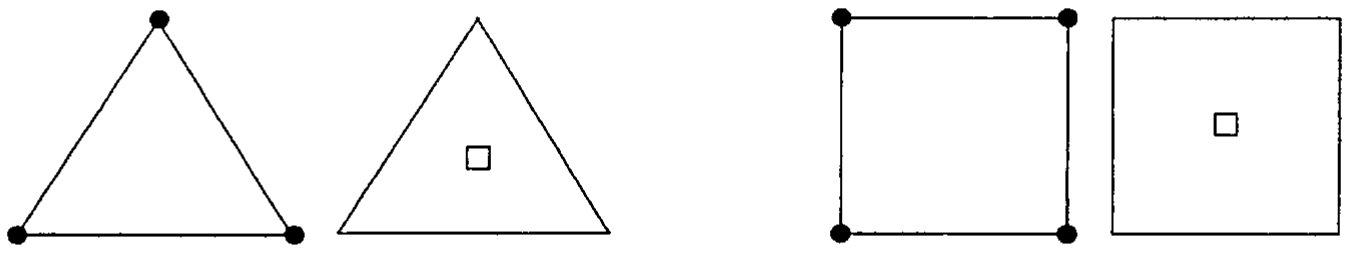
\includegraphics[width=.739\paperwidth]{images/fig-9-3-1.png}
  \caption{分片常值压力与分片线性或双线性速度}\label{fig:9.3.1}
\end{figure}

这类单元一般不满足相容性条件\eqref{eq:9.2.9},还可能发生锁定.例如,设剖分由 \(N\) 个三角形组成,每个三角形都有一条边在 \(\partial\Omega\) 上,且所有三角形共用同一个顶点(见\figref{fig:9.3.2}).此时,\(\boldsymbol{u}_h\) 仅有两个自由度,即唯一的内部顶点上的两个速度分量,而 \(p_h\) 有 \(N-1\) 个自由度,因为压力平均值为零,故比单元数少一个.条件\eqref{eq:9.2.22}于是给出 \(\boldsymbol{u}_h\equiv0\).

\begin{figure}[!htbp]
  \centering
  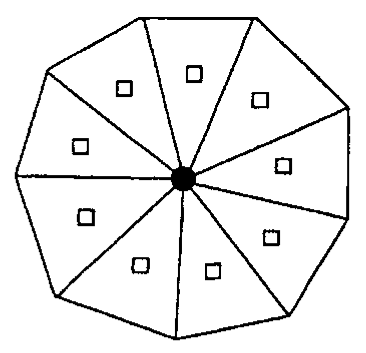
\includegraphics[width=.199\paperwidth]{images/fig-9-3-2.png}
  \caption{导致 \(\boldsymbol{u}_h\) 出现锁定现象的剖分}\label{fig:9.3.2}
\end{figure}

一种部分补救办法是采用所谓的交叉网格剖分.具体做法是将每个三角形 \(K\)(一个\emph{宏单元})分成三个以其重心为公共顶点的子三角形.压力在 \(K\) 上为常数,速度在每个子三角形上为线性函数,并在 \(\overline\Omega\) 上连续(见\figref{fig:9.3.3}).这样的选取消除了锁定现象,但仍不满足相容性条件\eqref{eq:9.2.9},例如见\BookCite{gunzburger1989}{Gunzburger(1989)}第 28 页.

\SourcePage{318}
\begin{figure}[!htbp]
  \centering
  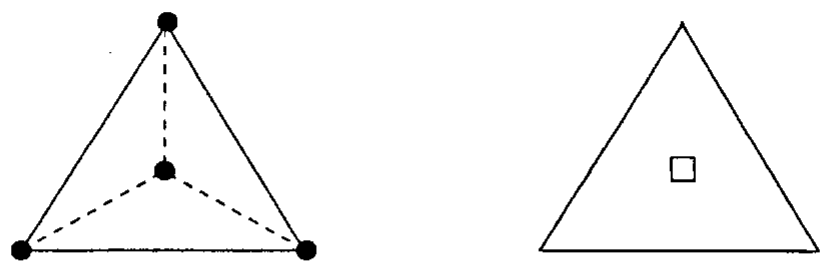
\includegraphics[width=.454\paperwidth]{images/fig-9-3-3.png}
  \caption{(交叉网格 \(\mathbb P_1\))--\(\mathbb P_0\) 单元}\label{fig:9.3.3}
\end{figure}

\figref{fig:9.3.1}右侧的分片 \(\mathbb Q_1\)--\(\mathbb Q_0\) 单元也未通过相容性检验.例如,设 \(\Omega\) 是边与坐标轴平行的矩形,并将它均匀剖分成矩形单元.可证明棋盘格模态在相邻单元上交替取 \(1\) 和 \(-1\)(必要时再减去平均值),由此得到的 \(p_h^*\in Q_h\) 确实是一个伪压力模态(见\BookCite{girault-raviart1986}{Girault 和 Raviart(1986)}第 160 页).

采用\figref{fig:9.3.4}左侧所示的交叉网格剖分,可以滤除该模态.用 \(\mathcal T_h\) 中任一平行四边形 \(K\)(宏单元)的两条对角线,将它分成四个三角形.相应空间是稳定的,并且有以下误差估计(见\BookCite{brezzi-fortin1991}{Brezzi 和 Fortin(1991)}第 VI.5.4 节)：
\begin{equation}\label{eq:9.3.5}
  \|\boldsymbol{u}-\boldsymbol{u}_h\|+\|p-p_h\|_0
       \le Ch(\|\boldsymbol{u}\|_2+\|p\|_1),
\end{equation}
其中 \(\|\cdot\|_s\) 是 \(s\) 阶 Sobolev 范数(见第~\ref{sec:1.2}~节),\(h\) 是宏单元直径的最大值.误差估计\eqref{eq:9.3.5}由\eqref{eq:9.2.11}、\eqref{eq:9.2.12}、定理~\ref{thm:3.4.2}以及估计\eqref{eq:3.5.24}得到,其中默认右端的两个范数均有意义.

\begin{figure}[!htbp]
  \centering
  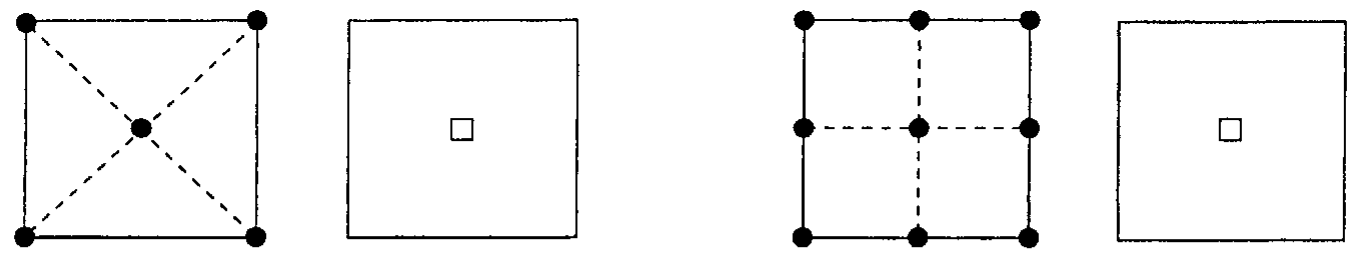
\includegraphics[width=.743\paperwidth]{images/fig-9-3-4.png}
  \caption{(交叉网格 \(\mathbb P_1\))--\(\mathbb Q_0\) 单元(左)和(交叉网格 \(\mathbb Q_1\))--\(\mathbb Q_0\) 单元(右)}\label{fig:9.3.4}
\end{figure}

另一种稳定化办法采用\figref{fig:9.3.4}右侧的宏单元.将每个平行四边形分成四个以其重心为公共顶点的平行四边形,然后在每个子单元上使用 \(\mathbb Q_1\) 多项式.这样的逼近稳定,且具有一阶收敛性(见\BookCite{gunzburger1989}{Gunzburger(1989)}第 30 页).

避免不稳定性的另一种办法是用更丰富的空间逼近速度.这里指出,\(\mathbb P_2\)--\(\mathbb P_0\) 和 \(\mathbb Q_2\)--\(\mathbb Q_0\) 单元都是稳定的,并且都具有一阶收敛性(\BookCite{fortin1972}{Fortin(1972)}).

为获得二阶精度,必须用分片线性多项式逼近压力.不过,\(\mathbb P_2\)--\(\mathbb P_1\) 单元,即在\eqref{eq:9.3.4}中取 \(k=2\) 和 \(m=1\) 所得的单元,仍不稳定(例如,见\BookCite{brezzi-fortin1991}{Brezzi 和 Fortin(1991)}第 231 页).可采用\BookCite{crouzeix-raviart1973}{Crouzeix 和 Raviart(1973)}引入的单元来实现稳定化.这类单元采用间断的分片 \(\mathbb P_1\) \SourcePage{319}压力和分片 \(\mathbb P_2^b(K)\) 速度,其中
\begin{equation}\label{eq:9.3.6}
  \mathbb P_k^b(K):=\{v=p_k+b\mid p_k\in\mathbb P_k,\
            b\text{ 是 }K\text{ 上的三次泡函数}\},\qquad k\ge1.
\end{equation}
三角形 \(K\) 上的三次\emph{泡函数} \(b\) 是在 \(K\) 的边上为零的三次多项式.因此,任一此类函数都可表示为下式的常数倍：
\begin{equation}\label{eq:9.3.7}
  b_K:=\lambda_1\lambda_2\lambda_3,
\end{equation}
其中 \(\{\lambda_i\mid i=1,2,3\}\) 为线性多项式,各自在 \(K\) 的一条边上为零,在对顶点取值 \(1\).泡函数由其在 \(K\) 的重心处的取值确定.Crouzeix--Raviart 单元稳定,且具有二阶收敛性.\figref{fig:9.3.5}左侧给出了它们的自由度.

Crouzeix--Raviart 单元的一种高阶推广采用间断的分片 \(\mathbb P_{k-1}\) 压力和分片 \(\mathbb P_k+B_{k+1}(K)\) 速度,其中在每个三角形 \(K\) 上,
\begin{equation}\label{eq:9.3.8}
  B_{k+1}(K):=\{v\in\mathbb P_{k+1}\mid v=p_{k-2}b_K,\
                    p_{k-2}\in\mathbb P_{k-2}\},\qquad k\ge2,
\end{equation}
而 \(b_K\) 由\eqref{eq:9.3.7}定义.因此,\(B_{k+1}\) 是 \(K\) 上次数不超过 \(k+1\) 的泡函数空间.这些单元满足相容性条件,且以 \(O(h^k)\) 的速率收敛.证明例如见\BookCite{girault-raviart1986}{Girault 和 Raviart(1986)}第 139 页.

\begin{figure}[!htbp]
  \centering
  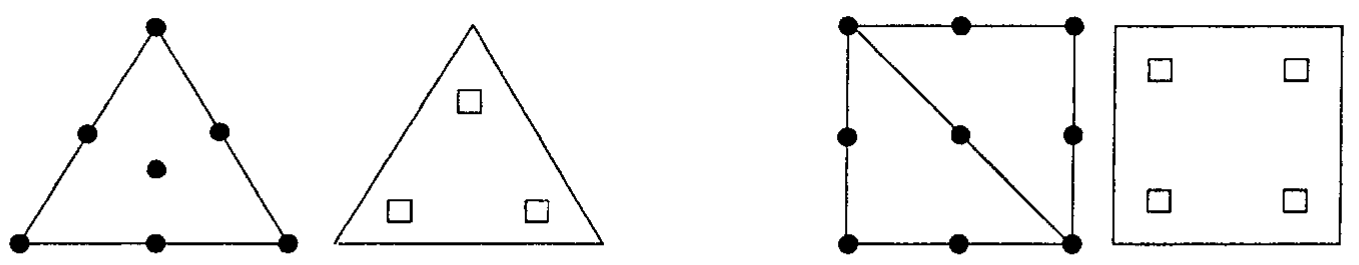
\includegraphics[width=.742\paperwidth]{images/fig-9-3-5.png}
  \caption{Crouzeix--Raviart 单元(左)和 Boland--Nicolaides 单元(右,\(k=2\))}\label{fig:9.3.5}
\end{figure}

另一个很好的例子以平行四边形为基础.采用间断的分片 \(\mathbb Q_{k-1}\) 压力(\(k\ge1\)),再沿各平行四边形的一条对角线将它分成两个三角形,速度在两个三角形上均为 \(\mathbb P_k\) 多项式.\figref{fig:9.3.5}右侧是 \(k=2\) 的例子.这类单元由\BookCite{boland-nicolaides1983}{Boland 和 Nicolaides(1983)}引入,满足相容性条件,且以 \(O(h^k)\) 的速率收敛(另见\BookCite{gunzburger1989}{Gunzburger(1989)}第 36 页).

其他稳定的单元还包括平行六面体剖分上的 \(\mathbb Q_2\)--\(\mathbb P_1\) 单元,其中压力仍是间断的.见\BookCite{girault-raviart1986}{Girault 和 Raviart(1986)}第 156 页.

\subsection{压力连续的有限元}\label{sec:9.3.2}
\SourcePage{320}

为简便起见,本小节也只考察二维情形.若要求有限元压力为连续函数,自然可考虑下列空间：
\begin{equation}\label{eq:9.3.9}
  Q_h=X_h^m\cap L_0^2(\Omega),\quad m\ge1,\qquad
  V_h=(X_h^k\cap H_0^1(\Omega))^2,\quad k\ge1.
\end{equation}

首先指出,所谓的\emph{等阶插值},即速度和压力采用相同多项式次数 \(m=k\),会给出不稳定的逼近.见\BookCite{sani-gresho-lee-griffiths1981}{Sani、Gresho、Lee 和 Griffiths(1981)}、\BookCite{sani-gresho-lee-griffiths-engelman1981}{Sani、Gresho、Lee、Griffiths 和 Engelman(1981)}以及\BookCite{brezzi-fortin1991}{Brezzi 和 Fortin(1991)}第 210 页.

\BookCite{taylor-hood1973}{Taylor 和 Hood(1973)}提出的单元对应\eqref{eq:9.3.9}中 \(m=1\)、\(k=2\) 的选择.这类单元稳定,并以最优速率收敛,即
\begin{equation}\label{eq:9.3.10}
  \|\boldsymbol{u}-\boldsymbol{u}_h\|+\|p-p_h\|_0
     \le Ch^s(\|\boldsymbol{u}\|_{s+1}+\|p\|_s),\qquad s=1,2,
\end{equation}
只要解具有足够的正则性,使右端的范数有意义(例如,见\BookCite{girault-raviart1986}{Girault 和 Raviart(1986)}第 176 页).这一结论对三角形单元和平行六面体型单元均成立.\BookCite{brezzi-falk1991}{Brezzi 和 Falk(1991)}分析了高阶 Taylor--Hood 单元,即\eqref{eq:9.3.9}中取 \(m=k-1\)、\(k\ge3\) 的情形.\figref{fig:9.3.6}给出 \(m=1\)、\(k=2\) 时的自由度.

\begin{figure}[!htbp]
  \centering
  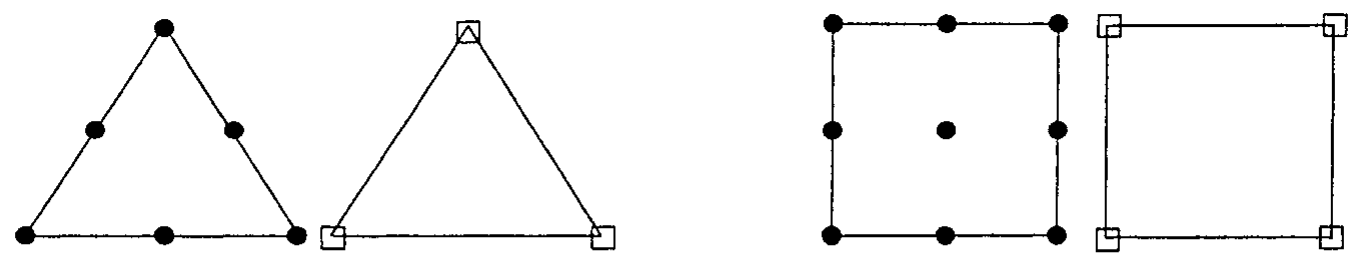
\includegraphics[width=.745\paperwidth]{images/fig-9-3-6.png}
  \caption{低阶 Taylor--Hood 三角形单元(左)和平行四边形单元(右)}\label{fig:9.3.6}
\end{figure}

另一种做法从由三角形 \(K\) 组成的剖分 \(\mathcal T_h\) 出发.压力在每个 \(K\) 上为线性函数,速度在 \(K\) 的三个以重心为公共顶点的子三角形上分片线性(见\figref{fig:9.3.7}左侧).为简便起见,记为(交叉网格 \(\mathbb P_1\))--\(\mathbb P_1\) 单元.这种选取满足相容性条件,相应的有限元解关于 \(h\) 一阶收敛(见\BookCite{pironneau1988}{Pironneau(1988)}第 107 页).

类似的思想产生了所谓的 \((\mathbb P_1\text{ iso }\mathbb P_2)\)--\(\mathbb P_1\) 单元,由\BookCite{bercovier-pironneau1979}{Bercovier 和 Pironneau(1979)}提出,见\figref{fig:9.3.7}右侧.压力空间仍相同,速度在 \(K\) 的四个子三角形上为线性函数,这四个子三角形由连接 \(K\) 各边的中点得到.此离散稳定,且具有一阶收敛性.\SourcePage{321}这种命名是因为其自由度与 \(\mathbb P_2\)--\(\mathbb P_1\) Taylor--Hood 单元的自由度相同(见\figref{fig:9.3.6}左侧).类似地,当 \(\mathcal T_h\) 由平行四边形组成时,可以考察 \((\mathbb Q_1\text{ iso }\mathbb Q_2)\)--\(\mathbb Q_1\) 单元.

\begin{figure}[!htbp]
  \centering
  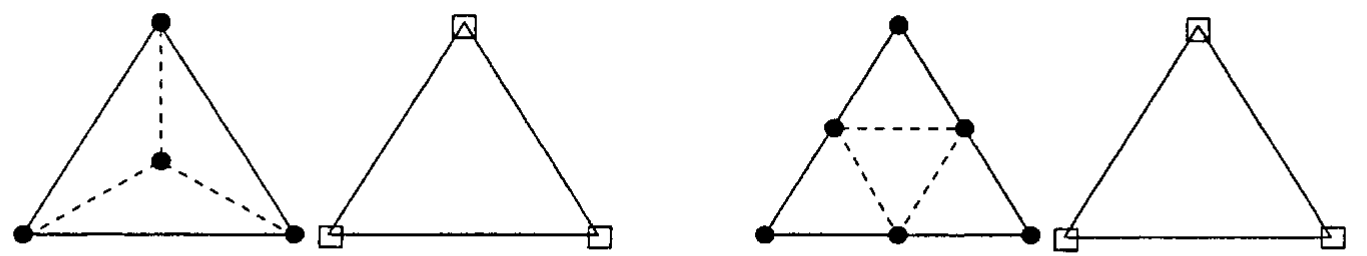
\includegraphics[width=.746\paperwidth]{images/fig-9-3-7.png}
  \caption{(交叉网格 \(\mathbb P_1\))--\(\mathbb P_1\) 单元(左)和 \((\mathbb P_1\text{ iso }\mathbb P_2)\)--\(\mathbb P_1\) 单元(右)}\label{fig:9.3.7}
\end{figure}

最后介绍所谓的 \emph{mini 单元},由\BookCite{arnold-brezzi-fortin1984}{Arnold、Brezzi 和 Fortin(1984)}引入.压力仍为分片 \(\mathbb P_1\) 函数,而速度为分片 \(\mathbb P_1^b\) 函数(见\eqref{eq:9.3.6}).这种选取稳定,并且一阶收敛(见\figref{fig:9.3.8}).mini 单元与\figref{fig:9.3.7}左侧的(交叉网格 \(\mathbb P_1\))--\(\mathbb P_1\) 单元十分相似.事实上,后者将 \(K\) 上在 \(\partial K\) 处为零的三次泡函数 \(b\),换成了同样在 \(\partial K\) 上为零的函数 \(\psi\in C^0(K)\).\(\psi\) 在以 \(K\) 的重心为公共顶点的三个子三角形上分别为线性函数.这两类单元具有相同的稳定性和收敛性质.

\begin{figure}[!htbp]
  \centering
  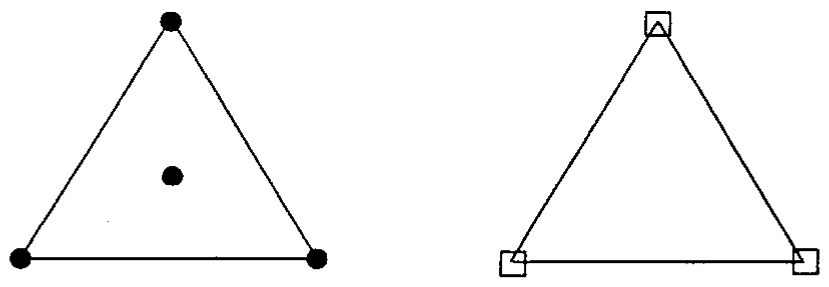
\includegraphics[width=.453\paperwidth]{images/fig-9-3-8.png}
  \caption{mini 单元}\label{fig:9.3.8}
\end{figure}

应用中还使用过许多其他有限元空间,例如速度非协调的单元以及基于降阶积分的单元.有兴趣的读者可参见\BookCite{girault-raviart1986}{Girault 和 Raviart(1986)}及\BookCite{brezzi-fortin1991}{Brezzi 和 Fortin(1991)}.

\section{稳定化方法}\label{sec:9.4}

若采用不满足相容性条件\eqref{eq:9.2.9}的空间对 \(V_h,Q_h\) 来构造鞍点问题\eqref{eq:9.1.11}的逼近\eqref{eq:9.2.4},离散解就可能受到伪压力模态的影响.可按多种准则对它作稳定化处理.

\SourcePage{322}第~\ref{sec:9.3}~节已经看到,有时采用交叉网格剖分,可以使一般剖分上原本不稳定的有限元变得稳定.

另一种稳定化办法并不依赖特殊剖分,而是略微修改\eqref{eq:9.2.4},并相应修改其代数方程组\eqref{eq:9.2.14}.这类方法通常旨在放宽不可压缩性约束,因此会改变\eqref{eq:9.2.4}的第二组方程.抽象地说,稳定化问题为
\begin{equation}\label{eq:9.4.1}
  \left\{
  \begin{aligned}
    &\text{求 }\boldsymbol{u}_h\in V_h,\ p_h\in Q_h,\ \text{使}\\
    &a(\boldsymbol{u}_h,\boldsymbol{v}_h)+b(\boldsymbol{v}_h,p_h)=(\boldsymbol{f},\boldsymbol{v}_h)
          &&\forall\,\boldsymbol{v}_h\in V_h,\\
    &b(\boldsymbol{u}_h,q_h)=\Phi_h(q_h)&&\forall\,q_h\in Q_h,
  \end{aligned}
  \right.
\end{equation}
其中稳定项 \(\Phi_h\) 线性地依赖于试验函数 \(q_h\),也可以依赖 \(\boldsymbol{u}_h\)、\(p_h\)、\(\boldsymbol{f}\) 及 \(h\).为简便起见,以下只考察二维问题.

\BookCite{brezzi-pitkaranta1984}{Brezzi 和 Pitkäranta(1984)}给出了第一个例子,取
\begin{equation}\label{eq:9.4.2}
  \Phi_h(q_h):=\sum_{K\in\mathcal T_h}h_K^2\int_K\nabla p_h\cdot\nabla q_h.
\end{equation}
这里仍以 \(\mathcal T_h\) 表示由三角形 \(K\) 构成的有限元剖分,\(h_K\) 是 \(K\) 的直径.第~\ref{sec:9.3.2}~节已经看到,若 \(\Phi_h\equiv0\),则\eqref{eq:9.3.9}中 \(m=k=1\) 的选择,即对压力和速度都使用连续分片线性多项式,会给出不稳定的逼近.把\eqref{eq:9.4.2}代入\eqref{eq:9.4.1},则得到稳定且一阶收敛的逼近.直观上,由于有 \(\Phi_h(q_h)\) 这一项,至少在\eqref{eq:9.4.2}中以 \(h\) 代替 \(h_K\) 时,可以把\eqref{eq:9.4.1}看作下列修正连续性方程的逼近：
\begin{equation}\label{eq:9.4.3}
  \operatorname{div}\boldsymbol{u}=h^2\Delta p,
\end{equation}
其中压力 \(p\) 满足齐次 Neumann 边界条件.关于这一方法的分析,另见\BookCite{brezzi-douglas1988}{Brezzi 和 Douglas(1988)}.

后来,\BookCite{hughes-franca-balestra1986}{Hughes、Franca 和 Balestra(1986)}建议,对于连续压力空间,采用
\begin{equation}\label{eq:9.4.4}
  \Phi_h(q_h):=\delta\sum_K h_K^2\int_K
      (a_0\boldsymbol{u}_h-\nu\Delta\boldsymbol{u}_h+\nabla p_h-\boldsymbol{f})\cdot\nabla q_h,
\end{equation}
并证明当 \(0<\delta\le C_I\) 时,方法是稳定的,其中 \(C_I\) 是一个适当常数.这一做法类似于第~\ref{sec:8.3.2}~节针对定常对流--扩散方程考察的流线迎风/Petrov--Galerkin(SUPG)法.若按\eqref{eq:9.3.9}取 \(m=k\),则速度和压力都以 \(O(h^k)\) 收敛.这时,在微分方程层次上,若所有 \(K\in\mathcal T_h\) 的 \(h_K\) 都等于 \(h\),连续性方程改为
\SourcePage{323}
\[
  \operatorname{div}\boldsymbol{u}
    =\delta h^2\operatorname{div}(a_0\boldsymbol{u}-\nu\Delta\boldsymbol{u}+\nabla p-\boldsymbol{f}).
\]
由\eqref{eq:9.1}可知,右端恒为零.实践中,参数 \(\delta\) 不能太小,否则无法消除寄生模态.另一方面,\(\delta\) 过大又会使 \(\partial\Omega\) 附近的压力场逼近不佳.还要注意,\eqref{eq:9.4.4}给\eqref{eq:9.2.4}引入了非对称扰动.

另一种选择是用
\begin{equation}\label{eq:9.4.5}
  \Phi_h(q_h):=\delta\sum_K h_K^2\left\{
     \int_K(a_0\boldsymbol{u}_h+\nabla p_h-\boldsymbol{f})\cdot\nabla q_h
     -\int_{\partial K\cap\partial\Omega}\nu\Delta\boldsymbol{u}_h\cdot\boldsymbol{n}\,q_h
    \right\}
\end{equation}
代替\eqref{eq:9.4.4}(见\BookCite{brezzi-douglas1988}{Brezzi 和 Douglas(1988)}).在各单元取相同权重时,对无散度向量 \(\boldsymbol{u}\),若 \(\Delta\boldsymbol{u}\) 连续,则\eqref{eq:9.4.4}和\eqref{eq:9.4.5}一致.这可由 Green 公式\eqref{eq:5.1.5}得到.与\eqref{eq:9.4.4}相比,\eqref{eq:9.4.5}的好处是,矩阵\eqref{eq:9.2.16}的扰动中,涉及 \(\boldsymbol{u}_h\) 的自由度仅限于与边界单元有关的那些自由度.

更一般的办法是同时扰动连续性方程和动量方程.稳定化问题为
\begin{equation}\label{eq:9.4.6}
  \left\{
  \begin{aligned}
    &\text{求 }\boldsymbol{u}_h\in V_h,\ p_h\in Q_h,\ \text{使}\\
    &a(\boldsymbol{u}_h,\boldsymbol{v}_h)+b(\boldsymbol{v}_h,p_h)
       =(\boldsymbol{f},\boldsymbol{v}_h)-\Psi_h^{(\rho)}(\boldsymbol{v}_h)
            &&\forall\,\boldsymbol{v}_h\in V_h,\\
    &b(\boldsymbol{u}_h,q_h)=\Phi_h(q_h)&&\forall\,q_h\in Q_h,
  \end{aligned}
  \right.
\end{equation}
其中 \(\Phi_h(q_h)\) 由\eqref{eq:9.4.4}给出,且
\[
  \begin{aligned}
  \Psi_h^{(\rho)}(\boldsymbol{v}_h):={}&\delta\sum_K h_K^2\int_K
      (a_0\boldsymbol{u}_h-\nu\Delta\boldsymbol{u}_h+\nabla p_h-\boldsymbol{f})\\
      &\hspace{9em}\cdot(\rho a_0\boldsymbol{v}_h-\rho\nu\Delta\boldsymbol{v}_h),
  \end{aligned}
\]
\(\rho\) 是一个参数,通常取 \(-1,0,1\),且 \(\delta>0\).

当 \(\rho=0\) 时,这一方法与 SUPG 法\eqref{eq:9.4.4}一致.当 \(\rho=-1\) 时,称为 Galerkin/最小二乘(GALS)法(\BookCite{hughes-franca1987}{Hughes 和 Franca(1987)}),所得方程组对称.\(\rho=1\) 的情形由\BookCite{douglas-wang1989}{Douglas 和 Wang(1989)}提出,所得方程组不对称.将连续性方程反号后,其双线性形式为半正定,并在更一般的条件下保持稳定.事实上,有下列结果(\BookCite{franca-stenberg1991}{Franca 和 Stenberg(1991)}).

\begin{theorem}[]{9.4.1}
设 \(V_h=(X_h^k\cap H_0^1(\Omega))^2\)、\(Q_h=Y_h^m\cap L_0^2(\Omega)\),其中 \(k\ge2\)、\(m\ge0\).对于 SUPG 和 GALS 法,即分别取 \(\rho=0\) 和 \(\rho=-1\),再假设
\SourcePage{324}
\begin{equation}\label{eq:9.4.7}
  0<\delta<C_I,
\end{equation}
其中 \(C_I\) 是适当常数.则\eqref{eq:9.4.6}给出稳定解,并且有下列最优收敛结果：
\begin{equation}\label{eq:9.4.8}
  \|\boldsymbol{u}-\boldsymbol{u}_h\|+\|p-p_h\|_0
       \le C(h^k\|\boldsymbol{u}\|_{k+1}+h^{m+1}\|p\|_{m+1}).
\end{equation}
当 \(k=1\) 时,只要对某个 \(m\ge1\) 取 \(Q_h=X_h^m\cap L_0^2(\Omega)\),使 \(Q_h\subset C^0(\overline\Omega)\),同样的结论依然成立.
\end{theorem}

\eqref{eq:9.4.7}中的 \(C_I\) 可能很小.事实上,其取值受逆不等式\eqref{eq:6.3.21}中的常数约束.

值得注意的是,有些有限元对问题\eqref{eq:9.2.4}不稳定,用于扰动后问题\eqref{eq:9.4.6}时却是稳定的.其中包括 \(\mathbb P_1\)--\(\mathbb P_1\) 和 \(\mathbb Q_1\)--\(\mathbb Q_1\) 单元(见\figref{fig:9.4.1}).

\begin{figure}[!htbp]
  \centering
  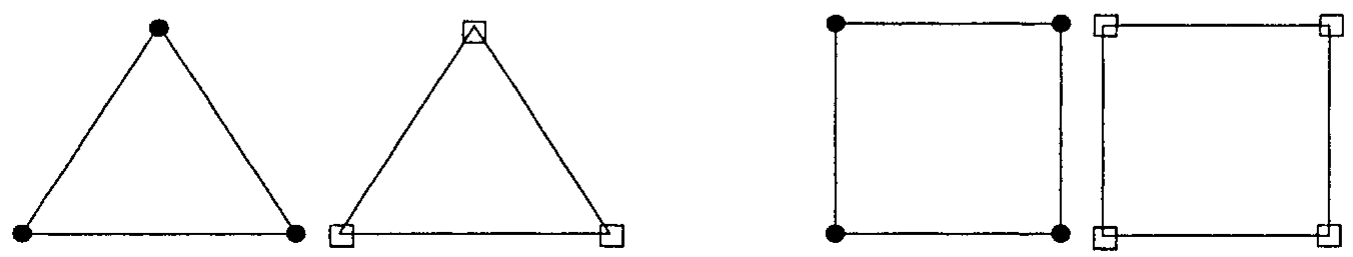
\includegraphics[width=.739\paperwidth]{images/fig-9-4-1.png}
  \caption{满足定理~\ref{thm:9.4.1}假设的有限元示例}\label{fig:9.4.1}
\end{figure}

\begin{note}\NumberedNote{note:9.4.1}
对于分片线性速度,或在矩形网格上的分片双线性速度,对所有 \(K\in\mathcal T_h\) 都有 \(\Delta\boldsymbol{v}_h|_K=0\).因此,在这一情形下,若再假定 \(a_0=0\),则本节迄今考察的各方法(\eqref{eq:9.4.2}除外)彼此一致.\hfill\(\square\)
\end{note}

前一个定理不适用于最低阶单元
\begin{equation}\label{eq:9.4.9}
  V_h=(X_h^1\cap H_0^1(\Omega))^2,\qquad Q_h=Y_h^0\cap L_0^2(\Omega)
\end{equation}
(见\figref{fig:9.3.1}).这类单元在一般剖分上仍可能有伪模态(见第~\ref{sec:9.3.1}~节).在这种情形下,一种稳定化方法如下：
\begin{equation}\label{eq:9.4.10}
  \left\{
  \begin{aligned}
    &\text{求 }\boldsymbol{u}_h\in V_h,\ p_h\in Q_h,\ \text{使}\\
    &a(\boldsymbol{u}_h,\boldsymbol{v}_h)+b(\boldsymbol{v}_h,p_h)=(\boldsymbol{f},\boldsymbol{v}_h)
       &&\forall\,\boldsymbol{v}_h\in V_h,\\
    &b(\boldsymbol{u}_h,q_h)=\delta\sum_{\sigma\in\Gamma_h}h_\sigma
          \int_\sigma[p_h]_\sigma[q_h]_\sigma &&\forall\,q_h\in Q_h,
  \end{aligned}
  \right.
\end{equation}
其中 \(\delta>0\) 是适当常数,\(\Gamma_h\) 是剖分中除边界 \(\partial\Omega\) 上的边以外的所有边的集合,\(h_\sigma\) 是 \(\sigma\) 的\SourcePage{325}长度.最后,对任意 \(q_h\in Q_h\),\([q_h]_\sigma\) 表示它跨边 \(\sigma\) 的跳跃.对于所有 \(\delta>0\),这一方法都给出稳定且一阶收敛的解,即
\[
  \|\boldsymbol{u}-\boldsymbol{u}_h\|+\|p-p_h\|_0\le Ch(\|\boldsymbol{u}\|_2+\|p\|_1)
\]
(\BookCite{kechkar-silvester1992}{Kechkar 和 Silvester(1992)}).

\eqref{eq:9.4.10}的代数表述给出如下对称、非奇异的方程组：
\begin{equation}\label{eq:9.4.11}
  \begin{pmatrix}A&B^T\\B&-\delta D\end{pmatrix}
     \begin{pmatrix}\boldsymbol{u}\\\boldsymbol{p}\end{pmatrix}
       =\begin{pmatrix}\boldsymbol{f}\\0\end{pmatrix},
\end{equation}
其中 \(D\) 为对称半正定矩阵,元素为
\begin{equation}\label{eq:9.4.12}
  D_{ij}:=\sum_{\sigma\in\Gamma_h}h_\sigma\int_\sigma[\psi_i]_\sigma[\psi_j]_\sigma.
\end{equation}
从代数上看,记\eqref{eq:9.4.11}中的矩阵为 \(S_\delta\),则可分解为
\[
  S_\delta=
  \begin{pmatrix}A&0\\B&I\end{pmatrix}
  \begin{pmatrix}A^{-1}&0\\0&-BA^{-1}B^T-\delta D\end{pmatrix}
  \begin{pmatrix}A&B^T\\0&I\end{pmatrix}.
\]
因此,由 Sylvester 惯性定律,\(S_\delta\) 的正、负特征值个数与第二个因子的相同,即有 \(N_h\) 个正特征值和 \(K_h\) 个负特征值.回顾一下,若 \(\ker B^T\ne\{0\}\),则\eqref{eq:9.2.16}中的矩阵 \(S\) 有 \(N_h\) 个正特征值,其余 \(K_h\) 个特征值为负或为零.

若剖分由\emph{宏单元}组成,且每个宏单元含四个三角形或四边形(见\figref{fig:9.4.2}),便可简化\eqref{eq:9.4.10}.其中关于 \(\sigma\in\Gamma_h\) 的求和可只取每个宏单元的内部边.简化后的格式与\eqref{eq:9.4.10}具有相同的稳定性和收敛性,而 \(D\) 的带宽更小.

\begin{figure}[!htbp]
  \centering
  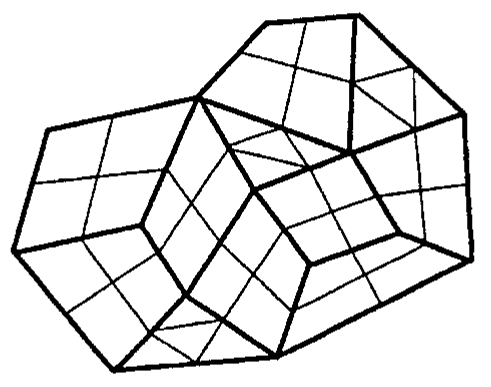
\includegraphics[width=.268\paperwidth]{images/fig-9-4-2.png}
  \caption{\(\Omega\) 的宏单元剖分}\label{fig:9.4.2}
\end{figure}

\begin{note}\NumberedNote{note:9.4.2}{\heiti(稳定化与泡函数)}
\BookCite{baiocchi-brezzi-franca1993}{Baiocchi、Brezzi 和 Franca(1993)}指出,在有限元空间中加入泡函数,可以得到一种在形式上类似于前述方法的稳定化方法(另见\SourcePage{326}\BookCite{pierre1988}{Pierre(1988}、\BookCite{pierre1989}{1989)}及\BookCite{bank-welfert1990}{Bank 和 Welfert(1990)}).类似的结论也适用于第~\ref{sec:8.3.2}~节引入的对流--扩散问题稳定化方法(见第~\ref{sec:8.3.3}~节).

用抽象的方式,可将采用泡函数空间的有限维方法表述如下.令
\[
  \mathcal V_h^b:=\mathcal U_h\oplus\mathcal B,
\]
其中 \(\mathcal U_h\) 是标准有限元空间,\(\mathcal B\) 是泡函数空间.例如,对\figref{fig:9.3.8}中的 mini 单元,有
\begin{equation}\label{eq:9.4.13}
  \mathcal U_h=(X_h^1\cap H_0^1(\Omega))^2\times(X_h^1\cap L_0^2(\Omega)),
      \qquad \mathcal B|_K=(B_3(K))^2\times\{0\}
\end{equation}
(见\eqref{eq:9.3.8}).然后,以 \(\mathcal A(\cdot,\cdot)\) 表示边值问题对应的双线性形式.有限维问题可表述为
\begin{equation}\label{eq:9.4.14}
  \begin{aligned}
    \text{求 }\boldsymbol{u}_h+\boldsymbol{u}_B\in\mathcal V_h^b,\quad\text{使}\quad
     \mathcal A(\boldsymbol{u}_h+\boldsymbol{u}_B,\boldsymbol{v}_h+\boldsymbol{v}_B)
       &=\mathcal F(\boldsymbol{v}_h+\boldsymbol{v}_B)\\
       &\qquad\forall\,\boldsymbol{v}_h\in\mathcal U_h,\ \boldsymbol{v}_B\in\mathcal B.
  \end{aligned}
\end{equation}
特别地,取 \(\boldsymbol{v}_h=0\),有
\[
  \mathcal A(\boldsymbol{u}_h+\boldsymbol{u}_B,\boldsymbol{v}_B)
       =\mathcal F(\boldsymbol{v}_B)\qquad\forall\,\boldsymbol{v}_B\in\mathcal B.
\]
逐单元计算 \(\boldsymbol{u}_B\),得到
\begin{equation}\label{eq:9.4.15}
  \boldsymbol{u}_B=\boldsymbol{\Phi}(\boldsymbol{f},\boldsymbol{u}_h),
\end{equation}
其中 \(\boldsymbol{\Phi}\) 是适当的映射.现在,在\eqref{eq:9.4.14}中取 \(\boldsymbol{v}_B=0\),可得
\begin{equation}\label{eq:9.4.16}
  \mathcal A(\boldsymbol{u}_h,\boldsymbol{v}_h)
    =\mathcal F(\boldsymbol{v}_h)-\mathcal A(\boldsymbol{\Phi}(\boldsymbol{f},\boldsymbol{u}_h),\boldsymbol{v}_h)
         \qquad\forall\,\boldsymbol{v}_h\in\mathcal U_h .
\end{equation}
这一问题就是在原空间 \(\mathcal U_h\) 上表述的 Galerkin 逼近.右端第二项可以看作旨在使解 \(\boldsymbol{u}_h\) 稳定的扰动.以 mini 单元为例,泡函数产生的效果可视为在空间 \(\mathcal U_h\) 上作 GALS 逼近.\hfill\(\square\)
\end{note}

\begin{note}\NumberedNote{note:9.4.3}
稳定化问题\eqref{eq:9.4.6}可写成类似于第~\ref{sec:8.3.2}~节对流--扩散方程的方法.事实上,若将 Stokes 算子和右端写为
\begin{equation}\label{eq:9.4.17}
  L(\boldsymbol{w},r):=\begin{pmatrix}a_0\boldsymbol{w}-\nu\Delta\boldsymbol{w}+\nabla r\\
                \operatorname{div}\boldsymbol{w}\end{pmatrix},
   \qquad \boldsymbol{f}^*:=\begin{pmatrix}\boldsymbol{f}\\0\end{pmatrix},
\end{equation}
则 \(L\) 关于 \(L^2(\Omega)\) 内积的对称部分和斜对称部分为
\SourcePage{327}
\begin{equation}\label{eq:9.4.18}
  L_S(\boldsymbol{w},r):=\begin{pmatrix}a_0\boldsymbol{w}-\nu\Delta\boldsymbol{w}\\0\end{pmatrix},
   \qquad L_{SS}(\boldsymbol{w},r):=\begin{pmatrix}\nabla r\\\operatorname{div}\boldsymbol{w}\end{pmatrix}.
\end{equation}
于是,可引入如下稳定化问题：求 \((\boldsymbol{u}_h,p_h)\in V_h\times Q_h\),使
\begin{equation}\label{eq:9.4.19}
  \begin{aligned}
    &a(\boldsymbol{u}_h,\boldsymbol{v}_h)+b(\boldsymbol{v}_h,p_h)-b(\boldsymbol{u}_h,q_h)\\
    &\quad+\delta\sum_{K\in\mathcal T_h}
        (L(\boldsymbol{u}_h,p_h)-\boldsymbol{f}^*,h_K^2(L_{SS}+\rho L_S)(\boldsymbol{v}_h,q_h))_K\\
    &\quad=(\boldsymbol{f},\boldsymbol{v}_h)
  \end{aligned}
\end{equation}
对每个 \((\boldsymbol{v}_h,q_h)\in V_h\times Q_h\) 成立.这与\eqref{eq:9.4.6}基本相同,事实上只在\eqref{eq:9.4.19}左端增加了稳定项
\[
  \delta\sum_{K\in\mathcal T_h}h_K^2(\operatorname{div}\boldsymbol{u}_h,\operatorname{div}\boldsymbol{v}_h)_K.
\]

注意,对流--扩散方程的 GALS 法对应 \(\rho=1\),Stokes 问题的 GALS 法则对应 \(\rho=-1\).这一名称对应的参数发生变化,是因为 GALS 法最初从 Stokes 算子的对称形式出发,即
\[
  L^*(\boldsymbol{w},r):=\begin{pmatrix}a_0\boldsymbol{w}-\nu\Delta\boldsymbol{w}+\nabla r\\
                    -\operatorname{div}\boldsymbol{w}\end{pmatrix}
\]
(见\BookCite{hughes-franca1987}{Hughes 和 Franca(1987)}),再从方程左端减去“最小二乘”项
\[
  \delta\sum_K h_K^2(a_0\boldsymbol{u}_h-\nu\Delta\boldsymbol{u}_h+\nabla p_h-\boldsymbol{f},\
                    a_0\boldsymbol{v}_h-\nu\Delta\boldsymbol{v}_h+\nabla q_h)_K .
\]
这对应于\eqref{eq:9.4.19}中 \(\rho=-1\) 的选择.事实上,对 Stokes 问题而言,将“最小二乘法”这一名称用于\eqref{eq:9.4.6}中 \(\rho=1\) 的 Douglas--Wang 法会更贴切.\hfill\(\square\)
\end{note}

\section{谱方法逼近}\label{sec:9.5}

这类逼近的特点是,试验函数和近似解都用高次代数多项式表示.为简便起见,假定 \(\Omega=(-1,1)^d\),\(d=2,3\).对于更一般的区域,需要采用区域分解方法,例如见第~\ref{sec:6.4}~节.

先逼近问题\eqref{eq:9.1.6},取
\begin{equation}\label{eq:9.5.1}
  V_N:=(\mathbb Q_N^0)^d,\qquad
  V_{\mathrm{div},N}:=\{\boldsymbol{v}_N\in V_N\mid\operatorname{div}\boldsymbol{v}_N=0\},
\end{equation}
\SourcePage{328}其中,仍以 \(\mathbb Q_N^0\) 记关于每个变量 \(x_i\)(\(i=1,\ldots,d\))的次数均不超过 \(N\)、在 \(\partial\Omega\) 上为零的代数多项式空间.此时,Galerkin 逼近\eqref{eq:9.2.1}写成
\begin{equation}\label{eq:9.5.2}
  \text{求 }\boldsymbol{u}_N\in V_{\mathrm{div},N},\quad\text{使}\quad
      a(\boldsymbol{u}_N,\boldsymbol{v}_N)=(\boldsymbol{f},\boldsymbol{v}_N)
       \qquad\forall\,\boldsymbol{v}_N\in V_{\mathrm{div},N}.
\end{equation}
这一问题存在唯一解,解是稳定的,并满足\eqref{eq:9.2.3}的收敛结论,只需相应改变记号.为得到关于 \(N^{-1}\) 的收敛阶,需要估计\eqref{eq:9.2.3}右端的下确界.为此,使用\BookCite{sacchilandriani-vandeven1989}{Sacchi Landriani 和 Vandeven(1989)}证明的下列结果.

\begin{theorem}[]{9.5.1}
对任意 \(s\ge1\),都存在与 \(N\) 无关的常数 \(C\),使对所有 \(\boldsymbol{v}\in(H^s(\Omega))^d\cap V_{\mathrm{div}}\),有
\begin{equation}\label{eq:9.5.3}
  \inf_{\boldsymbol{v}_N\in V_{\mathrm{div},N}}\|\boldsymbol{v}-\boldsymbol{v}_N\|
    \le CN^{1-s}\|\boldsymbol{v}\|_s.
\end{equation}
\end{theorem}

\begin{proof}
只考察二维情形(\(d=2\)).首先,对任意 \(\boldsymbol{v}\in V_{\mathrm{div}}\),存在{\heiti 流函数} \(\psi\in H^2(\Omega)\),使
\begin{equation}\label{eq:9.5.4}
  \boldsymbol{v}=\operatorname{rot}\psi:=
     \left(\frac{\partial\psi}{\partial x_2},-\frac{\partial\psi}{\partial x_1}\right)
       \qquad\text{在 }\Omega\text{ 内}.
\end{equation}
此外,若 \(\boldsymbol{v}\in(H^s(\Omega))^2\),其中 \(s\ge1\),则 \(\psi\in H^{s+1}(\Omega)\),选定其加性常数后有
\begin{equation}\label{eq:9.5.5}
  \|\psi\|_{s+1}\le C\|\boldsymbol{v}\|_s.
\end{equation}
由于 \(\boldsymbol{v}=0\) 在 \(\partial\Omega\) 上成立,\(\nabla\psi\) 在 \(\partial\Omega\) 上为零.此外,\(\psi\) 只确定到一个加性常数,可以令它在一个边界点处为零,从而它在整个 \(\partial\Omega\) 上恒为零.因此,\(\psi\in H_0^2(\Omega)\),其中
\begin{equation}\label{eq:9.5.6}
  H_0^2(\Omega)=\left\{\varphi\in H^2(\Omega)\ \middle|\
      \varphi=\frac{\partial\varphi}{\partial n}=0\text{ 在 }\partial\Omega\text{ 上}\right\}.
\end{equation}
在这一空间上,可以定义算子 \(P_{2,N}^0\),将任意 \(H_0^2(\Omega)\) 中的函数,按 \(H^2(\Omega)\) 的内积,正交投影到次数不超过 \(N\)、且函数及其法向导数均在 \(\partial\Omega\) 上为零的多项式空间.沿用类似于推导 \(P_{1,N}^0\) 误差估计的论证(见第~\ref{sec:4.5.2}~节),可证明
\begin{equation}\label{eq:9.5.7}
  \|\psi-P_{2,N}^0\psi\|_2
       \le CN^{1-s}\|\psi\|_{s+1}\le CN^{1-s}\|\boldsymbol{v}\|_s,\qquad s\ge1,
\end{equation}
其中最后一个不等式由\eqref{eq:9.5.5}得到.取 \(\boldsymbol{v}_N=\operatorname{rot}(P_{2,N}^0\psi)\),并注意 \(\boldsymbol{v}_N\in V_{\mathrm{div},N}\),即得\eqref{eq:9.5.3}.\hfill\(\square\)
\end{proof}

\SourcePage{329}由\eqref{eq:9.2.3}和\eqref{eq:9.5.3}可知
\begin{equation}\label{eq:9.5.8}
  \|\boldsymbol{u}-\boldsymbol{u}_N\|\le CN^{1-s}\|\boldsymbol{u}\|_s,
\end{equation}
其中假定对某个 \(s\ge1\),有 \(\boldsymbol{u}\in(H^s(\Omega))^d\cap V_{\mathrm{div}}\).得到 \(\boldsymbol{u}_N\) 之后,问题是如何恢复具有同样最优精度的压力场 \(p_N\).这并不容易,不过有些情况下可以做到.特别可参见\BookCite{moser-moin-leonard1983}{Moser、Moin 和 Leonard(1983)}的方法及其推广(见\BookCite{pasquarelli-quarteroni-sacchilandriani1987}{Pasquarelli、Quarteroni 和 Sacchi Landriani(1987)}及\BookCite{pasquarelli1991}{Pasquarelli(1991)}).不过要注意,这一做法采用由 Chebyshev 多项式的线性组合构成的 \(V_{\mathrm{div},N}\) 基(见第~\ref{sec:4.5.1}~节).相应地,\eqref{eq:9.5.2}中的每个积分都要换成采用 Chebyshev 权函数的加权积分(见第~\ref{sec:4.5.1}~节).

一般来说,构造 \(V_{\mathrm{div},N}\) 的基和恢复压力场都比较困难,因此可以直接逼近鞍点问题\eqref{eq:9.1.11}.对这一问题,可以采用谱 Galerkin 法,也可以采用广义 Galerkin 法,后者往往与谱配置法等价.

\subsection{谱 Galerkin 逼近}\label{sec:9.5.1}

令 \(Q_N\) 和 \(V_N\) 分别为 \(L_0^2(\Omega)\) 和 \((H_0^1(\Omega))^d\) 的多项式子空间,考察\eqref{eq:9.1.11}的下列谱逼近：
\begin{equation}\label{eq:9.5.9}
  \left\{
  \begin{aligned}
    &\text{求 }\boldsymbol{u}_N\in V_N,\ p_N\in Q_N,\ \text{使}\\
    &a(\boldsymbol{u}_N,\boldsymbol{v}_N)+b(\boldsymbol{v}_N,p_N)=(\boldsymbol{f},\boldsymbol{v}_N)
         &&\forall\,\boldsymbol{v}_N\in V_N,\\
    &b(\boldsymbol{u}_N,q_N)=0&&\forall\,q_N\in Q_N.
  \end{aligned}
  \right.
\end{equation}
通常,\(V_N\) 取为\eqref{eq:9.5.1}定义的空间,这可以保证速度场具有形如\eqref{eq:9.5.8}的误差估计.相应地,本想取 \(Q_N=M_N\),其中 \(M_N:=\mathbb Q_N\cap L_0^2(\Omega)\).但这种选择不合适,因为 \(V_N,M_N\) 不满足相容性条件\eqref{eq:9.2.9}.因此,需要选取 \(M_N\) 的一个真子空间作为 \(Q_N\).

先定义
\begin{equation}\label{eq:9.5.10}
  S_N:=\{p_N^*\in\mathbb Q_N\mid b(\boldsymbol{v}_N,p_N^*)=0\quad
                  \forall\,\boldsymbol{v}_N\in V_N\},
\end{equation}
即 \(\mathbb Q_N\) 中由所有伪压力模态组成的子空间(见\eqref{eq:9.2.21}).再定义
\begin{equation}\label{eq:9.5.11}
  D_N:=\{\varphi_N\in\mathbb Q_N\mid
          \exists\,\boldsymbol{v}_N\in V_N,\ \operatorname{div}\boldsymbol{v}_N=\varphi_N\},
\end{equation}
即 \(V_N\) 在散度算子下的像.显然,关于 \(L^2(\Omega)\) 内积,\(D_N\) 是 \(S_N\) 在 \(\mathbb Q_N\) 中的正交补.\SourcePage{330}可以完整刻画空间 \(S_N\).先注意,可以取 \(S_N\) 在 \(\mathbb Q_N\) 中的任一补空间作为压力空间 \(Q_N\),即取任一满足
\begin{equation}\label{eq:9.5.12}
  \dim S_N+\dim Q_N=\dim\mathbb Q_N,\qquad S_N\cap Q_N=\{0\}
\end{equation}
的子空间 \(Q_N\subset\mathbb Q_N\),并以选取零平均值代表元的方式固定压力的加性常数.

下列结果刻画了二维逼近的伪模态空间,证明例如见\BookCite{bernardi-maday1992}{Bernardi 和 Maday(1992)}第 126–127 页.

\begin{theorem}[]{9.5.2}
设 \(\Omega=(-1,1)^2\) 且 \(N\ge3\).空间 \(S_N\) 的维数为 \(8\),它的一组基由下列多项式给出：
\begin{equation}\label{eq:9.5.13}
  \begin{gathered}
    1,\quad L_N(x_1),\quad L_N(x_2),\quad L_N(x_1)L_N(x_2),\quad
          L_N'(x_1)L_N'(x_2),\\
    L_N'(x_1)L_{N+1}'(x_2),\quad L_{N+1}'(x_1)L_N'(x_2),\quad
       L_{N+1}'(x_1)L_{N+1}'(x_2),
  \end{gathered}
\end{equation}
其中 \(\{L_k\mid k=0,1,\ldots\}\) 为第~\ref{sec:4.4.1}~节引入的 Legendre 多项式.
\end{theorem}

\begin{proof}
容易证明,\eqref{eq:9.5.13}中的每个函数都属于 \(S_N\).反过来,来证明 \(S_N\) 中任意函数 \(p_N^*\) 都可由上述多项式线性组合得到.注意,\(p_N^*\) 必须满足
\begin{equation}\label{eq:9.5.14}
  \int_\Omega p_N^*\left(\frac{\partial v_{N,1}}{\partial x_1}
                       +\frac{\partial v_{N,2}}{\partial x_2}\right)\mathrm d\boldsymbol{x}=0
        \qquad\forall\,\boldsymbol{v}_N=(v_{N,1},v_{N,2})\in V_N .
\end{equation}
先取 \(\boldsymbol{v}_N=(\varphi_{mn},0)\),再取 \(\boldsymbol{v}_N=(0,\varphi_{mn})\),其中
\[
  \varphi_{mn}(x_1,x_2)=(1-x_1^2)(1-x_2^2)L_m'(x_1)L_n'(x_2),
       \qquad1\le m,n\le N-1.
\]
由\eqref{eq:9.5.14}可得
\begin{equation}\label{eq:9.5.15}
  \begin{aligned}
    \int_\Omega p_N^*(\boldsymbol{x})L_m(x_1)(1-x_2^2)L_n'(x_2)\,\mathrm d\boldsymbol{x}
      &=\int_\Omega p_N^*(\boldsymbol{x})(1-x_1^2)L_m'(x_1)L_n(x_2)\,\mathrm d\boldsymbol{x}\\
      &=0 .
  \end{aligned}
\end{equation}
这里使用了 Legendre 多项式的 Sturm--Liouville 公式(见\eqref{eq:4.4.2})：
\begin{equation}\label{eq:9.5.16}
  \bigl((1-\xi^2)L_k'(\xi)\bigr)'=-k(k+1)L_k(\xi),\qquad -1<\xi<1.
\end{equation}
回顾(见\eqref{eq:6.2.20}),
\begin{equation}\label{eq:9.5.17}
  \varphi_k(\xi):=(1-\xi^2)L_k'(\xi),\qquad1\le k\le N-1,
\end{equation}
是在 \(\xi=\pm1\) 处为零、次数不超过 \(N\) 的一维多项式空间 \(\mathbb P_N^0\) 的一组基.由\eqref{eq:9.5.16}和\eqref{eq:4.4.6}可知,\(\mathbb P_N^0\) 在 \(\mathbb P_N\) 中的正交补由 \(L_N'(\xi)\) 和 \(L_{N+1}'(\xi)\) 张成.因此,由\eqref{eq:9.5.15}可知,\(p_N^*\) 可写成
\SourcePage{331}
\[
  \begin{aligned}
    p_N^*(x_1,x_2)={}&a_0(x_2)+a_N(x_2)L_N(x_1)\\
           &+b_N(x_1)L_N'(x_2)+b_{N+1}(x_1)L_{N+1}'(x_2),
  \end{aligned}
\]
也可写成
\[
  \begin{aligned}
    p_N^*(x_1,x_2)={}&c_0(x_1)+c_N(x_1)L_N(x_2)\\
           &+d_N(x_2)L_N'(x_1)+d_{N+1}(x_2)L_{N+1}'(x_1),
  \end{aligned}
\]
其中 \(a_0,a_N,\ldots,d_N,d_{N+1}\) 是次数不超过 \(N\) 的代数多项式.因此,\(p_N^*\) 可表示为\eqref{eq:9.5.13}中各多项式的线性组合.

还需证明\eqref{eq:9.5.13}中的八个多项式线性无关.为此,只需验证 \(\{1,L_N,L_N',L_{N+1}'\}\) 线性无关.假设
\[
  \alpha_0+\alpha_NL_N+\beta_NL_N'+\beta_{N+1}L_{N+1}'=0.
\]
由积分关系
\[
  \int_{-1}^{\xi}L_k(\eta)\,\mathrm d\eta
    =\frac{L_{k+1}(\xi)-L_{k-1}(\xi)}{2k+1},\qquad -1\le\xi\le1,\quad k\ge1,
\]
可用 \((2N+1)L_N+L_{N-1}'\) 替换 \(L_{N+1}'\).注意,\(L_N\) 与 \(L_N'\) 的奇偶性不同.比较替换后各多项式的次数 \(0,N,N-1,N-2\),容易得到
\(\alpha_0=\alpha_N=\beta_N=\beta_{N+1}=0\).\hfill\(\square\)
\end{proof}

等价地,上述定理表明,\(D_N\) 在 \(\mathbb Q_N\) 中的余维为 \(8\).

非常数伪模态的存在表明,取 \(Q_N=\mathbb Q_N\) 为压力空间不能满足相容性条件.取 \(Q_N=D_N\) 时,该条件当然成立.不过,\eqref{eq:9.2.9}中的最优常数 \(\beta\) 关于 \(N\) 没有一致的正下界.证明这一性质的重要一步依赖于下列结果,其证明见\BookCite{bernardi-maday1992}{Bernardi 和 Maday(1992)}第 130 页.

\begin{lemma}[]{9.5.1}
对任意 \(q_N\in D_N\),存在多项式 \(\boldsymbol{v}_N\in V_N\),使
\begin{align}
  \operatorname{div}\boldsymbol{v}_N&=q_N,\label{eq:9.5.18}\\
  \|\boldsymbol{v}_N\|&\le CN\|q_N\|_0.\label{eq:9.5.19}
\end{align}
\end{lemma}

由这一引理,对每个 \(q_N\in D_N\),可以找到 \(\boldsymbol{v}_N\in V_N\),使
\[
  |b(\boldsymbol{v}_N,q_N)|=
      \left|\int_\Omega q_N\operatorname{div}\boldsymbol{v}_N\,\mathrm d\boldsymbol{x}\right|
        =\int_\Omega q_N^2\,\mathrm d\boldsymbol{x}
        \ge CN^{-1}\|\boldsymbol{v}_N\|\|q_N\|_0.
\]
\SourcePage{332}因此,\((V_N,D_N)\) 满足相容性条件,且 \(\beta\) 的最优值不小于 \(CN^{-1}\).这个结果不能改进,因为在 \(N\to\infty\) 时,找不到一个满足\eqref{eq:9.2.9}且比 \(N^{-1}\) 趋零更慢的 \(\beta\).因此,当 \(V_N=(\mathbb Q_N^0)^2\) 且 \(Q_N=D_N\) 时,Stokes 问题的谱 Galerkin 逼近有
\begin{equation}\label{eq:9.5.20}
  \beta\asymp N^{-1}.
\end{equation}

不过,从能否一致逼近压力的角度看,选择 \(Q_N=D_N\) 作为压力空间并不合适.事实上,\(D_N\) 与多项式 \(L_N'(x_1)L_N'(x_2)\) 等正交,这意味着某些低次多项式无法包含在 \(D_N\) 中.因此,\(D_N\) 不适合用来逼近物理压力空间 \(L_0^2(\Omega)\) 中的所有函数.

\BookCite{bernardi-maday-metivet1987}{Bernardi、Maday 和 Métivet(1987)}给出了一个更合适的选择：取 \(Q_N\) 为 \(\mathbb Q_N\) 中与下列多项式正交的所有多项式所成的空间：
\[
  \begin{gathered}
    1,\quad L_N(x_1),\quad L_N(x_2),\quad L_N(x_1)L_N(x_2),\quad
         A_{N-1}(x_1)A_{N-1}(x_2),\\
    A_{N-1}(x_1)A_N(x_2),\quad A_N(x_1)A_{N-1}(x_2),\quad A_N(x_1)A_N(x_2),
  \end{gathered}
\]
其中
\[
  A_{N-1}:=L_N'-P_{\lfloor\lambda N\rfloor}L_N',\qquad
  A_N:=P_{N-1}L_{N+1}'-P_{\lfloor\lambda N\rfloor}L_{N+1}'.
\]
对任意 \(0<\lambda<1\),\(\lfloor\lambda N\rfloor\) 表示 \(\lambda N\) 的整数部分,\(P_{\lfloor\lambda N\rfloor}\) 表示关于\eqref{eq:4.4.5}所定义的内积到次数不超过 \(\lfloor\lambda N\rfloor\) 的一维多项式空间上的正交投影.

这个选择看上去比较复杂,但从理论上很合适,因为相容性条件成立,且常数 \(\beta\) 与\eqref{eq:9.5.20}具有相同的渐近行为.此外,按上述准则选取的 \(Q_N\) 足够丰富,包含所有次数不超过 \(\lfloor\lambda N\rfloor\) 且平均值为零的多项式.因此,\(Q_N\) 具有最优的逼近性质.事实上,利用\eqref{eq:9.2.12}并结合\eqref{eq:9.5.20},得到下列压力误差估计：
\begin{equation}\label{eq:9.5.21}
  \|p-p_N\|_0\le CN^{2-s}(\|\boldsymbol{u}\|_s+\|p\|_{s-1}),\qquad s\ge2,
\end{equation}
其中假定精确解 \((\boldsymbol{u},p)\) 具有右端所要求的光滑性.注意,\eqref{eq:9.5.21}与最优估计相差一个因子 \(N\),它正是常数 \(\beta\) 的倒数的量级.

\subsection{谱配置逼近}\label{sec:9.5.2}
\SourcePage{333}

用谱方法逼近 Stokes 方程时,通常较多采用配置法.理由之一是\eqref{eq:9.5.9}的右端难以计算,配置法用 Gauss 数值积分代替所有积分,克服了这一困难.

令 \(\Omega=(-1,1)^2\),取整数 \(N\ge3\).以 \(\Omega_N\) 记全部 \((N+1)^2\) 个 Legendre--Gauss--Lobatto 节点(见\eqref{eq:4.5.38}),以 \(\Xi_N\) 记 \(\Omega_N\) 中属于 \(\Omega\) 内部的 \((N-1)^2\) 个节点,以 \(\Sigma_N\) 记位于边界 \(\partial\Omega\) 上的 \(4N\) 个节点.当 \(\Omega=(-1,1)^2\) 时,逼近\eqref{eq:9.1}的配置问题为
\begin{equation}\label{eq:9.5.22}
  \begin{cases}
    a_0\boldsymbol{u}_N-\nu\Delta\boldsymbol{u}_N+\nabla p_N=\boldsymbol{f},
      &\text{在 }\boldsymbol{x}\in\Xi_N\text{ 处},\\
    \operatorname{div}\boldsymbol{u}_N=0,&\text{在 }\boldsymbol{x}\in\Omega_N\setminus R_N\text{ 处},\\
    \boldsymbol{u}_N=0,&\text{在 }\boldsymbol{x}\in\Sigma_N\text{ 处},
  \end{cases}
\end{equation}
其中 \(R_N\) 是由八个节点组成的集合.其中四个是 \(\overline\Omega\) 的角点.其余四个记为 \(\{\boldsymbol{x}^1,\boldsymbol{x}^2,\boldsymbol{x}^3,\boldsymbol{x}^4\}\),可以任意选取,只要 Gram 矩阵 \((\phi_i(\boldsymbol{x}^j))_{i,j=1}^4\) 非奇异,其中
\(\phi_1(\boldsymbol{x})=1\)、\(\phi_2(\boldsymbol{x})=L_N(x_1)\)、\(\phi_3(\boldsymbol{x})=L_N(x_2)\)、\(\phi_4(\boldsymbol{x})=L_N(x_1)L_N(x_2)\).

利用离散内积\eqref{eq:4.5.39}和性质\eqref{eq:4.5.40},配置问题\eqref{eq:9.5.22}可等价地改写为
\begin{equation}\label{eq:9.5.23}
  \left\{
  \begin{aligned}
    &\text{求 }\boldsymbol{u}_N\in V_N,\ p_N\in Q_N,\ \text{使}\\
    &a_N(\boldsymbol{u}_N,\boldsymbol{v}_N)+b_N(\boldsymbol{v}_N,p_N)
       =(\boldsymbol{f},\boldsymbol{v}_N)_N&&\forall\,\boldsymbol{v}_N\in V_N,\\
    &b_N(\boldsymbol{u}_N,q_N)=0&&\forall\,q_N\in Q_N .
  \end{aligned}
  \right.
\end{equation}
说明如下.\(V_N\) 是\eqref{eq:9.5.1}定义的空间,\(Q_N\) 的维数为 \((N+1)^2-8\),它是下列函数所张成的空间 \(S_N^c\) 的补空间：
\begin{equation}\label{eq:9.5.24}
  \begin{gathered}
    1,\quad L_N(x_1),\quad L_N(x_2),\quad L_N(x_1)L_N(x_2),\quad L_N'(x_1)L_N'(x_2),\\
    L_N'(x_1)x_2L_N'(x_2),\quad x_1L_N'(x_1)L_N'(x_2),\quad
           x_1L_N'(x_1)x_2L_N'(x_2).
  \end{gathered}
\end{equation}
此外,
\begin{equation}\label{eq:9.5.25}
  \begin{aligned}
    a_N(\boldsymbol{w}_N,\boldsymbol{v}_N)&:=a_0(\boldsymbol{w}_N,\boldsymbol{v}_N)_N
       +\nu(\nabla\boldsymbol{w}_N,\nabla\boldsymbol{v}_N)_N,\\
    b_N(\boldsymbol{v}_N,q_N)&:=-(q_N,\operatorname{div}\boldsymbol{v}_N)_N,
  \end{aligned}
\end{equation}
其中 \((\cdot,\cdot)_N\) 是\eqref{eq:4.4.14}所定义的离散内积在二维情形下的推广,且 \(\boldsymbol{w}_N,\boldsymbol{v}_N\in V_N\)、\(q_N\in Q_N\).

因此,问题\eqref{eq:9.5.23}是\eqref{eq:9.1.11}的一个广义 Galerkin 逼近.与 Galerkin 情形一样,可使 \(Q_N\) 包含 \(\mathbb Q_{\lfloor\lambda N\rfloor}\) 中的零平均值多项式,其中 \(0<\lambda<1\).

\SourcePage{334}对于这种方法,可以直接证明推广了定理~\ref{thm:7.4.2}和定理~\ref{thm:7.4.3}的稳定性与收敛性定理.特别地,此时相容性条件为
\begin{equation}\label{eq:9.5.26}
  \forall\,q_N\in Q_N,\ \exists\,\boldsymbol{v}_N\in V_N,\ \boldsymbol{v}_N\ne0:\quad
    (q_N,\operatorname{div}\boldsymbol{v}_N)_N
       \ge\beta\|\boldsymbol{v}_N\|\|q_N\|_0 .
\end{equation}
采用上述有限维子空间时,\eqref{eq:9.5.23}没有非平凡的伪压力模态,也就是没有满足
\begin{equation}\label{eq:9.5.27}
  p_N^*\in Q_N,\qquad (p_N^*,\operatorname{div}\boldsymbol{v}_N)_N=0
             \qquad\forall\,\boldsymbol{v}_N\in V_N
\end{equation}
的非零函数 \(p_N^*\).仿照 Galerkin 情形,可以证明\eqref{eq:9.5.26}成立,且常数 \(\beta\) 与\eqref{eq:9.5.20}具有相同的渐近行为.这里也可得到类似于\eqref{eq:9.5.8}和\eqref{eq:9.5.21}的误差估计,只是多了一个涉及右端 \(\boldsymbol{f}\) 的项.具体来说,新的估计为
\begin{equation}\label{eq:9.5.28}
  \|\boldsymbol{u}-\boldsymbol{u}_N\|
    \le C\bigl(N^{1-s}\|\boldsymbol{u}\|_s+N^{-r}\|\boldsymbol{f}\|_r\bigr)
\end{equation}
和
\begin{equation}\label{eq:9.5.29}
  \|p-p_N\|_0
    \le C\bigl(N^{2-s}(\|\boldsymbol{u}\|_s+\|p\|_{s-1})+N^{1-r}\|\boldsymbol{f}\|_r\bigr),
\end{equation}
其中 \(s\ge2\)、\(r\ge2\) 要使右端的范数有意义.还可证明,这一逼近具有 \(\operatorname{div}\boldsymbol{u}_N\equiv0\) 的性质.

这一方法的算法实现见\BookCite{bernardi-maday1992}{Bernardi 和 Maday(1992)}第 153–155 页.

\subsection{谱广义 Galerkin 逼近}\label{sec:9.5.3}

这一方法由\BookCite{maday-meiron-patera-ronquist1993}{Maday、Meiron、Patera 和 Rønquist(1993)}提出,它不再与配置法等价.仍取 \(V_N=(\mathbb Q_N^0)^2\),但此时 \(Q_N=\mathbb Q_{N-2}\cap L_0^2(\Omega)\).谱问题为
\begin{equation}\label{eq:9.5.30}
  \left\{
  \begin{aligned}
    &\text{求 }\boldsymbol{u}_N\in V_N,\ p_N\in Q_N,\ \text{使}\\
    &a_N(\boldsymbol{u}_N,\boldsymbol{v}_N)+b(\boldsymbol{v}_N,p_N)
      =(\boldsymbol{f},\boldsymbol{v}_N)_N &&\forall\,\boldsymbol{v}_N\in V_N,\\
    &b(\boldsymbol{u}_N,q_N)=0&&\forall\,q_N\in Q_N,
  \end{aligned}
  \right.
\end{equation}
其中 \(a_N(\cdot,\cdot)\) 由\eqref{eq:9.5.25}定义,\(b(\cdot,\cdot)\) 由\eqref{eq:9.1.10}定义.由 Legendre--Gauss--Lobatto 求积公式的精确性,以及 \(Q_N\) 中多项式的次数不超过 \(N-2\),可得
\[
  b(\boldsymbol{v}_N,q_N)=-(\operatorname{div}\boldsymbol{v}_N,q_N)_N=b_N(\boldsymbol{v}_N,q_N)
       \qquad\forall\,\boldsymbol{v}_N\in V_N,\ q_N\in Q_N.
\]
由此,根据\eqref{eq:9.5.30}有
\SourcePage{335}
\[
  \begin{aligned}
    a_0\boldsymbol{u}_N-\nu\Delta\boldsymbol{u}_N+\nabla p_N&=\boldsymbol{f}
             &&\text{在 }\boldsymbol{x}\in\Xi_N\text{ 处},\\
    \boldsymbol{u}_N&=0&&\text{在 }\boldsymbol{x}\in\Sigma_N\text{ 处}.
  \end{aligned}
\]
此外,对任意 \(\boldsymbol{x}=(\xi_i,\xi_j)\in\Xi_N\),\(\operatorname{div}\boldsymbol{u}_N(\boldsymbol{x})\) 是 \(\operatorname{div}\boldsymbol{u}_N\) 在四个点 \((-1,\xi_j)\)、\((1,\xi_j)\)、\((\xi_i,-1)\)、\((\xi_i,1)\) 处的值的一个适当线性组合.这说明\eqref{eq:9.5.30}不是完全配置法.

这一方法的好处是,压力空间 \(Q_N\) 易于刻画,而且没有伪模态.此外,可以证明
\begin{equation}\label{eq:9.5.31}
  \forall\,q_N\in Q_N,\ \exists\,\boldsymbol{v}_N\in V_N,\ \boldsymbol{v}_N\ne0:\quad
     b(\boldsymbol{v}_N,q_N)\ge CN^{-1/2}\|\boldsymbol{v}_N\|\|q_N\|_0,
\end{equation}
即相容性条件成立,且可取 \(N^{-1/2}\) 量级的常数 \(\beta\).因此,在通常的光滑性假设下,误差估计为
\begin{equation}\label{eq:9.5.32}
  \begin{aligned}
    \|\boldsymbol{u}-\boldsymbol{u}_N\|+N^{-1/2}\|p-p_N\|_0
       &\le C\bigl[N^{1-s}(\|\boldsymbol{u}\|_s+\|p\|_{s-1})
                     +N^{-r}\|\boldsymbol{f}\|_r\bigr],
  \end{aligned}
\end{equation}
优于\eqref{eq:9.5.29}.

\section{Stokes 方程组的求解}\label{sec:9.6}

这里讨论如何求解 Stokes 方程组\eqref{eq:9.2.14}.将要考察的有些方法实际上以微分方程组的另一种表述为基础,再对重新表述后的方程组作逼近,因而所得数值解未必与\eqref{eq:9.2.14}的数值解一致.

回顾一下,矩阵 \(S\) 对称但不定.若 \(\ker B^T=\{0\}\),它就是非奇异的；而相容性条件\eqref{eq:9.2.9}成立时,正是这种情形.下面介绍文献中受到较多关注的求解技术.关于有限元逼近,更完整的综述例如见\BookCite{pironneau1988}{Pironneau(1988)}、\BookCite{gunzburger1989}{Gunzburger(1989)}、\BookCite{quartapelle1993}{Quartapelle(1993)}及\BookCite{fortin1993}{Fortin(1993)}；关于谱逼近,见\BookCite{canuto-hussaini-quarteroni-zang1988}{Canuto、Hussaini、Quarteroni 和 Zang(1988)}、\BookCite{boyd1989}{Boyd(1989)}和\BookCite{ronquist1988}{Rønquist(1988)}.

本节沿用同一个记号 \(\boldsymbol{u}\),既表示无限维问题\eqref{eq:9.1}的解,即向量函数 \(\boldsymbol{u}=\boldsymbol{u}(\boldsymbol{x})\),也表示线性方程组\eqref{eq:9.2.14}的解,即有限维向量 \(\boldsymbol{u}\in\mathbb R^{N_h}\).

\subsection{压力矩阵法}\label{sec:9.6.1}
\SourcePage{336}

这一方法以\eqref{eq:9.2.17}和\eqref{eq:9.2.18}中的消元过程为基础.消去速度向量后,得到一个单独关于压力的线性方程组：
\begin{equation}\label{eq:9.6.1}
  R\boldsymbol{p}=\boldsymbol{g},
\end{equation}
其中 \(R\) 是\eqref{eq:9.2.19}给出的 \(K_h\times K_h\) 压力矩阵,\(\boldsymbol{g}=BA^{-1}\boldsymbol{f}\).前面已经指出,\(R\) 对称,并且在 \(\ker B^T=\{0\}\) 时正定.

若\eqref{eq:9.1}中 \(a_0=0\),则对满足一致相容性条件的离散,压力矩阵在质量矩阵 \(J\) 所给出的度量下条件良好.事实上,\(\nu R\) 是算子 \(\operatorname{div}\Delta^{-1}\nabla\) 的一个逼近,而该算子的行为类似于恒等算子.因此,\(\nu R\) 接近恒等算子的变分对应物,即压力质量矩阵 \(J:=(\psi_l,\psi_m)_{lm}\)(见\eqref{eq:9.2.15}).更准确地说,用 \(\chi_{sp}\) 表示谱条件数(见\eqref{eq:2.4.8}),则
\begin{equation}\label{eq:9.6.2}
  \chi_{sp}(J^{-1}R)
     =\frac{\lambda_{\max}(J^{-1}R)}{\lambda_{\min}(J^{-1}R)}
     =\frac{\delta_h^2}{\beta_h^2},
\end{equation}
其中 \(\beta_h\) 和 \(\delta_h\) 是在 \(A\) 所诱导的速度范数下,\eqref{eq:9.2.9}和\eqref{eq:9.2.8}中的最优常数(见第~\ref{sec:9.2.1}~节及\BookCite{fortin-pierre1992}{Fortin 和 Pierre(1992)}).若 \(\beta_h\) 有与 \(h\) 无关的正下界,则这一谱条件数也有与 \(h\) 无关的上界.在 \(J\) 谱等价于标量倍单位矩阵的基下,同样可以控制 \(\chi_{sp}(R)\).

在这些情形下,共轭梯度法可以高效求解\eqref{eq:9.6.1},其收敛速率与 \(R\) 的阶数无关,见第~\ref{sec:2.4.2}~节.每次共轭梯度迭代的关键步骤是求残差
\[
  \boldsymbol{r}^k=\boldsymbol{g}-R\boldsymbol{p}^k,
\]
可以按如下顺序完成：
\begin{enumerate}[label=(\roman*)]
  \item 先计算 \(\boldsymbol{q}^k=B^T\boldsymbol{p}^k\).
  \item 再求解 \(A\boldsymbol{y}^k=\boldsymbol{q}^k\).
  \item 最后计算 \(\boldsymbol{r}^k=\boldsymbol{g}-B\boldsymbol{y}^k\).
\end{enumerate}
步骤 (i) 和 (iii) 很简单,只需作矩阵与向量的乘法.步骤 (ii) 则需要求解系数矩阵相同的线性方程组,二维时有两个,每个都是一个速度分量的 Poisson 问题.由于 \(A\) 对称正定,可以用直接法(对 \(A\) 作 Cholesky 分解)或内层共轭梯度迭代来完成步骤 (ii),见第~\ref{ch:2}~章.后一种情形下,应对 \(A\) 进行预处理,因为 \(A\) 的条件数随其阶数 \(N_h\) 增长(见\eqref{eq:6.3.17}和\eqref{eq:6.3.25}).还应注意,这样求解步骤 (ii) 可能代价较高,因为在对 \(R\) 作外层迭代的每一步中,都要将计算向量 \(\boldsymbol{y}^k\) 的内层迭代进行到收敛.第~\BookRef{sec:9.6.7}{9.6.7}~节将介绍没有这一缺点的方法.

对谱逼近而言,相容性条件中的常数 \(\beta\) 有时依赖于多项式解的\SourcePage{337}次数 \(N\)(见\eqref{eq:9.5.20}和\eqref{eq:9.5.31}).即使如此,通常仍采用外层共轭梯度迭代求解\eqref{eq:9.6.1},可以不作预处理,也可以取 \(J/\nu\) 为预条件矩阵.

当\eqref{eq:9.1}中的 \(a_0\ne0\) 时,例如在时间依赖问题中,压力矩阵 \(R\) 的条件数可能随离散尺度恶化,尤其是 \(a_0\) 相对于扩散项很大时.速度矩阵 \(A\) 的谱条件数也会随离散维数增大,例如在二维情形,有限元情形可按 \(N_h\) 增长,谱逼近情形可按 \(N_h^2\) 增长.因此,宜为方程组\eqref{eq:9.6.1}选取预条件矩阵 \(P\).下面回顾几种已经提出的选法.

首先,从\eqref{eq:9.1}形式上可推出,压力 \(p\) 满足
\[
  \begin{cases}
    -\Delta p=-\operatorname{div}\boldsymbol{f},&\text{在 }\Omega\text{ 内},\\
    \dfrac{\partial p}{\partial n}
      =\boldsymbol{f}\cdot\boldsymbol{n}+\nu\Delta\boldsymbol{u}\cdot\boldsymbol{n}
        -a_0\boldsymbol{u}\cdot\boldsymbol{n},&\text{在 }\partial\Omega\text{ 上}.
  \end{cases}
\]
由于 \(\boldsymbol{u}=0\) 在 \(\partial\Omega\) 上成立,在 \(\nu\) 很小时略去 \(\nu\Delta\boldsymbol{u}\cdot\boldsymbol{n}\),便得到一个在 \(\partial\Omega\) 上带 Neumann 边界条件的 Poisson 问题.因此,可以取 \(P\) 为与 Neumann 条件下 Laplace 算子对应的 \(K_h\times K_h\) 矩阵.

这一选法由\BookCite{benque-ibler-keramsi-labadie1980}{Benqué、Ibler、Keramsi 和 Labadie(1980)}提出,后来由\BookCite{cahouet-chabard1988}{Cahouet 和 Chabard(1988)}推广.他们建议用算子 \((\nu I^{-1}-a_0\Delta^{-1})^{-1}\) 的适当逼近作为 \(P\),其中仍采用 Neumann 边界条件.在离散层次,这相当于选取预条件矩阵
\[
  P=(\nu J^{-1}+a_0H^{-1})^{-1},
\]
其中 \(H:=BM^{-1}B^T\),\(M_{ij}:=(\boldsymbol{\varphi}_i,\boldsymbol{\varphi}_j)\) 为速度质量矩阵(见\eqref{eq:9.2.15}).这样选取时,\(P^{-1}R\) 是算子
\[
  -(\nu I^{-1}-a_0\Delta^{-1})
        \operatorname{div}(a_0I-\nu\Delta)^{-1}\nabla
\]
的一个逼近.这个算子在 \(\nu=0\) 或 \(a_0=0\) 时的行为类似于恒等算子.数值试验表明,至少对满足相容性条件\eqref{eq:9.2.9}的有限元逼近,\(P^{-1}R\) 的谱条件数与有限元网格尺寸无关(见\BookCite{cahouet-chabard1988}{Cahouet 和 Chabard(1988)}).

稍一般的办法是采用 \((\mu_1I^{-1}-\mu_2\Delta^{-1})^{-1}\) 的一个逼近,其中 \(\mu_1,\mu_2\) 根据 Stokes 问题所给边界条件的类型选取.

\subsection{Uzawa 法}\label{sec:9.6.2}

这一方法来自对原问题\eqref{eq:9.1}的下列迭代过程.给定 \(p^0\),对任意 \(k\ge0\),求解
\SourcePage{338}
\begin{equation}\label{eq:9.6.3}
  a_0\boldsymbol{u}^{k+1}-\nu\Delta\boldsymbol{u}^{k+1}=\boldsymbol{f}-\nabla p^k,
\end{equation}
其中 \(\boldsymbol{u}^{k+1}=0\) 在 \(\partial\Omega\) 上成立,然后令
\begin{equation}\label{eq:9.6.4}
  p^{k+1}-p^k=-\rho\operatorname{div}\boldsymbol{u}^{k+1}.
\end{equation}
正实数 \(\rho\) 是一个加速参数.适当选取 \(\rho\) 时,这一过程正是对鞍点泛函\eqref{eq:9.1.12}的对偶泛函应用梯度法.还要注意,可以把\eqref{eq:9.6.4}看作伪演化连续性方程
\[
  \frac{\partial p}{\partial t}+\operatorname{div}\boldsymbol{u}=0
\]
的向后 Euler 逼近,其中 \(\rho\) 相当于时间步长 \(\Delta t\).

在离散层次,Uzawa 格式就是以压力质量矩阵 \(J\) 为预条件矩阵,对方程\eqref{eq:9.6.1}应用预处理 Richardson 法(见第~\ref{sec:2.4.1}~节).

当 \(0<\rho<2\nu\) 时,\eqref{eq:9.6.3}、\eqref{eq:9.6.4}收敛.证明例如见\BookCite{temam1984}{Temam(1984)}.不过,它通常收敛较慢,可以在\eqref{eq:9.6.4}中使用与上一小节所讨论的同类型的压力矩阵 \(R\) 的预条件矩阵 \(P\) 来加快收敛.预处理迭代的代数形式为
\begin{equation}\label{eq:9.6.5}
  \begin{cases}
    A\boldsymbol{u}^{k+1}=\boldsymbol{f}-B^T\boldsymbol{p}^k,\\
    P(\boldsymbol{p}^{k+1}-\boldsymbol{p}^k)=\rho B\boldsymbol{u}^{k+1}.
  \end{cases}
\end{equation}
这一迭代法的收敛速率通常与网格尺寸 \(h\) 无关.

\subsection{Arrow--Hurwicz 法}\label{sec:9.6.3}

下面给出一个较复杂的格式,但每次迭代的计算量与 Uzawa 法相同.给定 \(p^0\) 和 \(\boldsymbol{u}^0\),对 \(k\ge0\),求解
\begin{equation}\label{eq:9.6.6}
  \begin{aligned}
    \beta_0\boldsymbol{u}^{k+1}-\Delta\boldsymbol{u}^{k+1}
       &=\beta_0\boldsymbol{u}^k-\Delta\boldsymbol{u}^k\\
       &\quad+\rho(\boldsymbol{f}-\nabla p^k-a_0\boldsymbol{u}^k+\nu\Delta\boldsymbol{u}^k),
  \end{aligned}
\end{equation}
其中 \(\boldsymbol{u}^{k+1}=0\) 在 \(\partial\Omega\) 上成立,然后令
\begin{equation}\label{eq:9.6.7}
  p^{k+1}-p^k=-\frac{\rho}{\sigma}\operatorname{div}\boldsymbol{u}^{k+1}.
\end{equation}
选取参数 \(\beta_0\ge0\)、\(\rho>0\) 和 \(\sigma>0\),使迭代收敛.常用的一种简单选取是 \(\beta_0=a_0/\nu\).简化情形 \(\beta_0=a_0=0\) 下的收敛性证明,例如见\BookCite{temam1984}{Temam(1984)}.一般情形的证明类似,当 \(a_0>0\) 且
\[
  0<\rho<\min\left(\frac{2\beta_0}{a_0},\frac{2\sigma\nu}{1+\sigma\nu^2}\right)
\]
时得到收敛性.

\SourcePage{339}还应注意,可以用其他对称且具有强制性的预条件算子代替 \(\beta_0I-\Delta\).在离散层次,通常可采用矩阵 \(A/\nu\) 的适当对称正定预条件矩阵 \(P\).

\subsection{罚方法}\label{sec:9.6.4}

另一种方法是所谓的\emph{罚方法}.它将待极小化的泛函改为
\begin{equation}\label{eq:9.6.8}
  \mathcal I_\varepsilon(\boldsymbol{v})
    :=\frac{a_0}{2}\int_\Omega|\boldsymbol{v}|^2+\frac{\nu}{2}\int_\Omega|\nabla\boldsymbol{v}|^2
       +\frac{1}{2\varepsilon}\int_\Omega|\operatorname{div}\boldsymbol{v}|^2
       -(\boldsymbol{f},\boldsymbol{v}),
\end{equation}
其中 \(\varepsilon>0\),极小化在 \((H_0^1(\Omega))^d\) 上进行.

这相当于求解
\begin{equation}\label{eq:9.6.9}
  \begin{cases}
    a_0\boldsymbol{u}_\varepsilon-\nu\Delta\boldsymbol{u}_\varepsilon
       -\dfrac1\varepsilon\nabla\operatorname{div}\boldsymbol{u}_\varepsilon=\boldsymbol{f},
        &\text{在 }\Omega\text{ 内},\\
    \boldsymbol{u}_\varepsilon=0,&\text{在 }\partial\Omega\text{ 上},
  \end{cases}
\end{equation}
或等价地求解
\begin{equation}\label{eq:9.6.10}
  \begin{cases}
    a_0\boldsymbol{u}_\varepsilon-\nu\Delta\boldsymbol{u}_\varepsilon+\nabla p_\varepsilon
       =\boldsymbol{f},&\text{在 }\Omega\text{ 内},\\
    \boldsymbol{u}_\varepsilon=0,&\text{在 }\partial\Omega\text{ 上},\\
    \varepsilon p_\varepsilon+\operatorname{div}\boldsymbol{u}_\varepsilon=0,
       &\text{在 }\Omega\text{ 内}.
  \end{cases}
\end{equation}
约束 \(\operatorname{div}\boldsymbol{u}=0\) 不再精确满足.不过,可以证明,当 \(\varepsilon\to0\) 时,\(\boldsymbol{u}_\varepsilon\) 和 \(p_\varepsilon\) 以一阶精度收敛到\eqref{eq:9.1}的解(例如,见\BookCite{bercovier1978}{Bercovier(1978)}及\BookCite{temam1984}{Temam(1984)}).但必须注意,\eqref{eq:9.6.9}对应矩阵的谱条件数按 \(1/\varepsilon\) 增长,而且恢复压力 \(p_\varepsilon\) 还需要另解一个与压力质量矩阵 \(J\) 对应的线性方程组.

另一种罚方法如下.对每个 \(\varepsilon>0\),求解下列问题的解 \((\boldsymbol{u}_\varepsilon^*,p_\varepsilon^*)\)：
\begin{equation}\label{eq:9.6.11}
  \begin{cases}
    a_0\boldsymbol{u}_\varepsilon^*-\nu\Delta\boldsymbol{u}_\varepsilon^*
      +\nabla p_\varepsilon^*=\boldsymbol{f},&\text{在 }\Omega\text{ 内},\\
    \boldsymbol{u}_\varepsilon^*=0,&\text{在 }\partial\Omega\text{ 上},\\
    -\varepsilon\Delta p_\varepsilon^*+\operatorname{div}\boldsymbol{u}_\varepsilon^*=0,
      &\text{在 }\Omega\text{ 内},\\
    \dfrac{\partial p_\varepsilon^*}{\partial n}=0,&\text{在 }\partial\Omega\text{ 上}.
  \end{cases}
\end{equation}
用 Galerkin 有限元法逼近\eqref{eq:9.6.11}会得到问题\eqref{eq:9.4.1}、\eqref{eq:9.4.2},其中以 \(\varepsilon\) 代替\eqref{eq:9.4.2}中的 \(h_K^2\).取 \(\varepsilon=h^2\),\BookCite{brezzi-pitkaranta1984}{Brezzi 和 Pitkäranta(1984)}的分析给出误差估计
\SourcePage{340}
\[
  \|\boldsymbol{u}-\boldsymbol{u}_h\|_1+\|p-p_h\|_0=O(h),
\]
其中 \(V_h\) 和 \(Q_h\) 按\eqref{eq:9.3.9}选取,取 \(k=m=1\).

再次强调,罚方法确实可以看作 Stokes 方程组的稳定化方法(见第~\ref{sec:9.4}~节).不过,由于精确解满足 \(\operatorname{div}\boldsymbol{u}=0\),这些格式不具有\eqref{eq:8.3.6}所定义的强相容性.

\subsection{增广 Lagrange 法}\label{sec:9.6.5}

这是 Uzawa 法和罚方法\eqref{eq:9.6.10}的结合.仍用微分形式来写,增广 Lagrange 迭代如下.给定 \(p^0\),对任意 \(k\ge0\),求解方程组
\begin{align}
  a_0\boldsymbol{u}^{k+1}-\nu\Delta\boldsymbol{u}^{k+1}+\nabla p^{k+1}
     &=\boldsymbol{f},\label{eq:9.6.12}\\
  p^{k+1}-p^k&=-\rho\operatorname{div}\boldsymbol{u}^{k+1},\label{eq:9.6.13}
\end{align}
并对 \(\boldsymbol{u}^{k+1}\) 施加边界条件.\(\rho\) 仍是一个加速参数.

\eqref{eq:9.6.13}的代数形式为
\begin{equation}\label{eq:9.6.14}
  J(\boldsymbol{p}^{k+1}-\boldsymbol{p}^k)=\rho B\boldsymbol{u}^{k+1},
\end{equation}
其中 \(J\) 是压力质量矩阵.在有限元逼近和谱 Galerkin 逼近中,\(J_{lm}=(\psi_l,\psi_m)\)(见\eqref{eq:9.2.15}).在谱配置法中,采用离散内积下归一化的压力基时,\(J\) 是单位矩阵.无论哪种情形,\(J\) 都非奇异,因而可以形式上消去 \(\boldsymbol{p}^{k+1}\),代入\eqref{eq:9.6.12},得到方程组
\begin{equation}\label{eq:9.6.15}
  (A+\rho B^TJ^{-1}B)\boldsymbol{u}^{k+1}=\boldsymbol{f}-B^T\boldsymbol{p}^k.
\end{equation}
这是一个对称正定方程组.求解后,例如采用预处理共轭梯度法,即可由\eqref{eq:9.6.14}恢复压力 \(\boldsymbol{p}^{k+1}\).

对任意 \(\rho>0\),\eqref{eq:9.6.12}和\eqref{eq:9.6.13}都收敛,且 \(\rho\) 很大时收敛很快(见\BookCite{fortin-pierre1992}{Fortin 和 Pierre(1992)}).但必须注意,随着 \(\rho\) 增大,\eqref{eq:9.6.15}中矩阵 \(A+\rho B^TJ^{-1}B\) 的谱条件数也增大(见\BookCite{fortin-glowinski1983}{Fortin 和 Glowinski(1983)}第 15 页).这里假定 \(\ker B\ne\{0\}\),这是得到非零速度逼近的必要条件.有时也把增广 Lagrange 法用作共轭梯度法求解问题\eqref{eq:9.2.14}的预处理(见\BookCite{fortin1989}{Fortin(1989)}).

关于增广 Lagrange 法的详细介绍,见\BookCite{glowinski-letallec1989}{Glowinski 和 Le Tallec(1989)}.

\subsection{基于压力求解器的方法}\label{sec:9.6.6}
\SourcePage{341}

对\eqref{eq:9.1}中的动量方程取散度,利用 \(\boldsymbol{u}\) 无散度,得到
\begin{equation}\label{eq:9.6.16}
  \Delta p=\operatorname{div}\boldsymbol{f}\qquad\text{在 }\Omega\text{ 内}.
\end{equation}
Poisson 问题\eqref{eq:9.6.16}需要给定 \(p\) 或其法向导数的边界条件.形式上,取动量方程在 \(\partial\Omega\) 上的法向分量,得到
\begin{equation}\label{eq:9.6.17}
  \frac{\partial p}{\partial n}=\boldsymbol{f}\cdot\boldsymbol{n}+\nu\Delta\boldsymbol{u}\cdot\boldsymbol{n}
          \qquad\text{在 }\partial\Omega\text{ 上},
\end{equation}
前提是这些项在 \(\partial\Omega\) 上有意义.

上式给出问题\eqref{eq:9.6.16}的一个 Neumann 条件,不过它将 \(\boldsymbol{u}\) 与 \(p\) 联系在一起.使 \(\partial\Omega\) 上的 \(\boldsymbol{u}\) 与 \(p\) 解耦的一种办法是采用下列迭代.给定满足 Neumann 相容性条件 \(\int_{\partial\Omega}\partial_np^0=\int_\Omega\operatorname{div}\boldsymbol{f}\) 的 \(p^0\),对每个 \(k\ge0\),先求解
\begin{equation}\label{eq:9.6.18}
  \begin{cases}
    a_0\boldsymbol{u}^{k+1}-\nu\Delta\boldsymbol{u}^{k+1}
       =\boldsymbol{f}-\nabla p^k,&\text{在 }\Omega\text{ 内},\\
    \boldsymbol{u}^{k+1}=0,&\text{在 }\partial\Omega\text{ 上},
  \end{cases}
\end{equation}
再求解
\begin{equation}\label{eq:9.6.19}
  \begin{cases}
    -\Delta p^{k+1}=-\operatorname{div}\boldsymbol{f},&\text{在 }\Omega\text{ 内},\\
    \dfrac{\partial p^{k+1}}{\partial n}
       =\boldsymbol{f}\cdot\boldsymbol{n}+\nu\Delta\boldsymbol{u}^{k+1}\cdot\boldsymbol{n},
       &\text{在 }\partial\Omega\text{ 上}.
  \end{cases}
\end{equation}

另一种可能是给\eqref{eq:9.6.16}施加压力的 Dirichlet 条件.首先注意,若 \((\boldsymbol{u},p)\) 是\eqref{eq:9.1}的经典解,则\eqref{eq:9.6.16}和
\begin{equation}\label{eq:9.6.20}
  \operatorname{div}\boldsymbol{u}=0\qquad\text{在 }\partial\Omega\text{ 上}
\end{equation}
都成立.反过来,若 \((\boldsymbol{u},p)\) 是\eqref{eq:9.1}中的动量方程和第三个条件以及\eqref{eq:9.6.16}、\eqref{eq:9.6.20}的经典解,则可立即验证
\[
  \begin{cases}
    a_0\operatorname{div}\boldsymbol{u}-\nu\Delta\operatorname{div}\boldsymbol{u}=0,
          &\text{在 }\Omega\text{ 内},\\
    \operatorname{div}\boldsymbol{u}=0,&\text{在 }\partial\Omega\text{ 上},
  \end{cases}
\]
因而必有 \(\operatorname{div}\boldsymbol{u}=0\) 在 \(\Omega\) 内成立.于是,\((\boldsymbol{u},p)\) 是 Stokes 问题\eqref{eq:9.1}的经典解.不过,\eqref{eq:9.6.20}不能直接作为 Poisson 问题\eqref{eq:9.6.16}的边界条件.下面介绍一种绕开这一困难的办法.

\SourcePage{342}基本思想是寻找 \(\partial\Omega\) 上的未知值 \(\lambda\),使 \(p=p(\lambda)\) 在满足边界条件
\begin{equation}\label{eq:9.6.21}
  p=\lambda\qquad\text{在 }\partial\Omega\text{ 上}
\end{equation}
时解出\eqref{eq:9.6.16},而 Dirichlet 问题
\begin{equation}\label{eq:9.6.22}
  \begin{cases}
    a_0\boldsymbol{u}(\lambda)-\nu\Delta\boldsymbol{u}(\lambda)
       =\boldsymbol{f}-\nabla p(\lambda),&\text{在 }\Omega\text{ 内},\\
    \boldsymbol{u}(\lambda)=0,&\text{在 }\partial\Omega\text{ 上}
  \end{cases}
\end{equation}
的解 \(\boldsymbol{u}=\boldsymbol{u}(\lambda)\) 满足\eqref{eq:9.6.20}.如果能够做到这一点,由前面的推导可知,\((\boldsymbol{u},p)\) 确实是\eqref{eq:9.1}的解.这一过程有几种实现方式.下面给出其中两种,即\emph{影响矩阵法}和\emph{积分条件法}.

先讨论影响矩阵法.设 \(H(\mu)\) 是边界值 \(\mu\) 的调和延拓,即下列问题的解：
\begin{equation}\label{eq:9.6.23}
  \begin{cases}
    \Delta H(\mu)=0,&\text{在 }\Omega\text{ 内},\\
    H(\mu)=\mu,&\text{在 }\partial\Omega\text{ 上}.
  \end{cases}
\end{equation}
\eqref{eq:9.6.16}、\eqref{eq:9.6.21}的解 \(p(\lambda)\) 可写成 \(p(\lambda)=H(\lambda)+p_0\),其中 \(p_0\) 满足
\begin{equation}\label{eq:9.6.24}
  \begin{cases}
    \Delta p_0=\operatorname{div}\boldsymbol{f},&\text{在 }\Omega\text{ 内},\\
    p_0=0,&\text{在 }\partial\Omega\text{ 上}.
  \end{cases}
\end{equation}
同样,可将\eqref{eq:9.6.22}的解 \(\boldsymbol{u}(\lambda)\) 分解为 \(\boldsymbol{u}(\lambda)=\widehat{\boldsymbol{u}}(\lambda)+\boldsymbol{u}_0\),其中
\begin{equation}\label{eq:9.6.25}
  \begin{cases}
    a_0\widehat{\boldsymbol{u}}(\lambda)-\nu\Delta\widehat{\boldsymbol{u}}(\lambda)
         =-\nabla H(\lambda),&\text{在 }\Omega\text{ 内},\\
    \widehat{\boldsymbol{u}}(\lambda)=0,&\text{在 }\partial\Omega\text{ 上},
  \end{cases}
\end{equation}
而且
\begin{equation}\label{eq:9.6.26}
  \begin{cases}
    a_0\boldsymbol{u}_0-\nu\Delta\boldsymbol{u}_0=\boldsymbol{f}-\nabla p_0,&\text{在 }\Omega\text{ 内},\\
    \boldsymbol{u}_0=0,&\text{在 }\partial\Omega\text{ 上}.
  \end{cases}
\end{equation}
再引入函数 \(\psi(\lambda)\),它是下列问题的解：
\begin{equation}\label{eq:9.6.27}
  \begin{cases}
    \Delta\psi(\lambda)=\operatorname{div}\boldsymbol{u}(\lambda),
         &\text{在 }\Omega\text{ 内},\\
    \psi(\lambda)=0,&\text{在 }\partial\Omega\text{ 上}.
  \end{cases}
\end{equation}
对\eqref{eq:9.6.22}中的第一个方程取散度,由\eqref{eq:9.6.16}和\eqref{eq:9.6.27}容易得到
\SourcePage{343}
\[
  a_0\Delta\psi(\lambda)-\nu\Delta^2\psi(\lambda)=0\qquad\text{在 }\Omega\text{ 内}.
\]
因此,若满足 \(\partial\psi(\lambda)/\partial n=0\) 在 \(\partial\Omega\) 上成立,则在 \(\Omega\) 内有 \(\psi(\lambda)=0\),从而 \(\operatorname{div}\boldsymbol{u}(\lambda)=0\).

形式上利用 Green 公式\eqref{eq:1.3.3}以及\eqref{eq:9.6.23}和\eqref{eq:9.6.27},对适当函数类 \(\Lambda\) 中的每个边界函数 \(\mu\),有
\[
  \begin{aligned}
    \int_{\partial\Omega}\frac{\partial\psi(\lambda)}{\partial n}\mu
      &=\int_\Omega\operatorname{div}[\nabla\psi(\lambda)H(\mu)]\\
      &=\int_\Omega\Delta\psi(\lambda)H(\mu)
           +\int_\Omega\nabla\psi(\lambda)\cdot\nabla H(\mu)\\
      &=\int_\Omega\operatorname{div}\boldsymbol{u}(\lambda)H(\mu)
           -\int_\Omega\psi(\lambda)\Delta H(\mu)\\
      &=\int_\Omega\operatorname{div}\boldsymbol{u}(\lambda)H(\mu).
  \end{aligned}
\]
由此便要求寻找 \(\lambda\in\Lambda\),使
\begin{equation}\label{eq:9.6.28}
  \int_\Omega\operatorname{div}\boldsymbol{u}(\lambda)H(\mu)=0\qquad\forall\,\mu\in\Lambda.
\end{equation}
再次使用 Green 公式\eqref{eq:1.3.3},可将\eqref{eq:9.6.28}等价地改写为
\begin{equation}\label{eq:9.6.29}
  \text{求 }\lambda\in\Lambda,\quad\text{使}\quad
   \mathcal A(\lambda,\mu)=\mathcal F(\mu)\qquad\forall\,\mu\in\Lambda,
\end{equation}
其中
\[
  \begin{aligned}
    \mathcal A(\eta,\mu)
      &:=a_0(\widehat{\boldsymbol{u}}(\eta),\widehat{\boldsymbol{u}}(\mu))
       +\nu(\nabla\widehat{\boldsymbol{u}}(\eta),\nabla\widehat{\boldsymbol{u}}(\mu)),\\
    \mathcal F(\mu)
      &:=-a_0(\boldsymbol{u}_0,\widehat{\boldsymbol{u}}(\mu))
       -\nu(\nabla\boldsymbol{u}_0,\nabla\widehat{\boldsymbol{u}}(\mu)).
  \end{aligned}
\]
形式 \(\mathcal A(\cdot,\cdot)\) 对称.此外,适当选取 \(\Lambda\) 时,可以证明 \(\mathcal A(\cdot,\cdot)\) 在 \(\Lambda\times\Lambda\) 上连续且具有强制性(见\BookCite{glowinski-pironneau1979}{Glowinski 和 Pironneau(1979)}或\BookCite{girault-raviart1986}{Girault 和 Raviart(1986)}第 183 页).因此,Lax--Milgram 引理保证\eqref{eq:9.6.29}有唯一解 \(\lambda\).

从数值角度看,问题\eqref{eq:9.6.29}的规模等于位于 \(\partial\Omega\) 上的网格点个数.例如,可以用共轭梯度法求解.得到 \(\partial\Omega\) 上的 \(\lambda\) 后,就可以逼近 Poisson 问题\eqref{eq:9.6.16}.最后,通过求解 Poisson 型问题\eqref{eq:9.6.22}恢复 \(\boldsymbol{u}\).从代数角度看,这相当于求解系数矩阵相同的线性方程组,二维时每个速度分量对应一个,共两个.

这一方法的详细分析和高效实现,有限元逼近情形见\BookCite{glowinski-pironneau1979}{Glowinski 和 Pironneau(1979)},另见\BookCite{chinosi-comodi1991}{Chinosi 和 Comodi(1991)}；谱逼近情形见\BookCite{kleiser-schumann1980}{Kleiser 和 Schumann(1980)}、\BookCite{canuto-sacchilandriani1986}{Canuto 和 Sacchi Landriani(1986)}以及\BookCite{sacchilandriani1987}{Sacchi Landriani(1987)}.

影响矩阵法得名于相应的矩阵：它把 \(\lambda\) 在 \(\partial\Omega\) 上各网格点处的值所成的向量,映到 \(\operatorname{div}\boldsymbol{u}(\lambda)\) 在同一组节点处的值所成的向量.

\SourcePage{344}积分条件法由\BookCite{quartapelle-napolitano1986}{Quartapelle 和 Napolitano(1986)}提出.其名称来自这样一个事实：在这一表述中,要求压力满足一个积分条件,这一条件在一定程度上起到压力边界条件的作用.推导如下.为明确起见,考虑三维情形.引入算子
\begin{equation}\label{eq:9.6.30}
  \operatorname{Curl}\boldsymbol{v}
     :=(D_2v_3-D_3v_2,\ D_3v_1-D_1v_3,\ D_1v_2-D_2v_1).
\end{equation}
容易验证
\[
  -\Delta\boldsymbol{v}=\operatorname{Curl}\operatorname{Curl}\boldsymbol{v}
                     -\nabla\operatorname{div}\boldsymbol{v}.
\]
因此,成立下列 Green 公式：
\begin{equation}\label{eq:9.6.31}
  \begin{aligned}
    -\int_\Omega\Delta\boldsymbol{w}\cdot\boldsymbol{v}
      &=\int_\Omega\bigl(\operatorname{div}\boldsymbol{w}\operatorname{div}\boldsymbol{v}
                        +\operatorname{Curl}\boldsymbol{w}\cdot\operatorname{Curl}\boldsymbol{v}\bigr)\\
      &\quad-\int_{\partial\Omega}\bigl[(\operatorname{div}\boldsymbol{w})\boldsymbol{v}\cdot\boldsymbol{n}
                 +(\operatorname{Curl}\boldsymbol{w})\cdot(\boldsymbol{n}\times\boldsymbol{v})\bigr].
  \end{aligned}
\end{equation}
令 \(\boldsymbol{K}(\mu)\) 为下列问题的解：
\begin{equation}\label{eq:9.6.32}
  \begin{cases}
    a_0\boldsymbol{K}(\mu)-\nu\Delta\boldsymbol{K}(\mu)=0,&\text{在 }\Omega\text{ 内},\\
    \boldsymbol{K}(\mu)\cdot\boldsymbol{n}=\mu,&\text{在 }\partial\Omega\text{ 上},\\
    \boldsymbol{K}(\mu)\times\boldsymbol{n}=0,&\text{在 }\partial\Omega\text{ 上}.
  \end{cases}
\end{equation}
利用\eqref{eq:9.6.31}和\eqref{eq:9.6.32},\eqref{eq:9.1}的解 \((\boldsymbol{u},p)\) 满足
\begin{equation}\label{eq:9.6.33}
  \begin{aligned}
    \int_\Omega\nabla p\cdot\boldsymbol{K}(\mu)
      &=\int_\Omega(\boldsymbol{f}-a_0\boldsymbol{u}+\nu\Delta\boldsymbol{u})\cdot\boldsymbol{K}(\mu)\\
      &=\int_\Omega\boldsymbol{f}\cdot\boldsymbol{K}(\mu)\qquad\forall\,\mu\in\Lambda .
  \end{aligned}
\end{equation}
由于这一积分关系必须对每个边界函数 \(\mu\) 成立,可以把它看作压力的一个边界条件.从\eqref{eq:9.6.33}出发,可建立一个变分问题,其解给出正确的压力边界值.像前面一样分解 \(p(\lambda)\) 后,求 \(\lambda\in\Lambda\),使
\begin{equation}\label{eq:9.6.34}
  \int_\Omega\nabla H(\lambda)\cdot\boldsymbol{K}(\mu)
   =\int_\Omega(\boldsymbol{f}-\nabla p_0)\cdot\boldsymbol{K}(\mu)\qquad\forall\,\mu\in\Lambda.
\end{equation}
这一问题代替了\eqref{eq:9.6.29}.注意,左端的双线性形式不对称.

利用\eqref{eq:9.6.25}和\eqref{eq:9.6.26}改写 \(\nabla H(\lambda)\) 和 \(\nabla p_0\),再对含 \(\widehat{\boldsymbol{u}}(\lambda)\) 和 \(\boldsymbol{u}_0\) 的项分部积分.由\eqref{eq:9.6.31}可知,若 \(\lambda\) 是\eqref{eq:9.6.34}的解,则对应的向量场 \(\boldsymbol{u}(\lambda)\) 满足
\begin{equation}\label{eq:9.6.35}
  \nu\int_{\partial\Omega}\operatorname{div}\boldsymbol{u}(\lambda)\mu=0\qquad\forall\,\mu\in\Lambda,
\end{equation}
\SourcePage{345}即 \(\operatorname{div}\boldsymbol{u}(\lambda)=0\) 在 \(\partial\Omega\) 上成立.

关于积分条件法的全面分析、高效实现及其与影响矩阵法的比较,见\BookCite{quartapelle1993}{Quartapelle(1993)}第 5.3–5.5 节.

\subsection{一种整体预处理技术}\label{sec:9.6.7}

对压力矩阵 \(R\) 施行共轭梯度迭代,或采用相当于对 \(R\) 作预处理 Richardson 迭代的 Uzawa 法,都有一个缺点：每一步迭代都必须计算 \(R\) 的作用,特别是 \(A^{-1}\) 的作用.

若采用双层迭代,即对\eqref{eq:9.6.1}用外层共轭梯度法,而对与 \(A\) 有关的方程组用内层迭代法,则因 \(A\) 的条件较差,应为其采用预条件矩阵,例如 \(P_0\).这样做的整体求解代价可能较高,因为每一步外层迭代都必须将内层迭代进行到收敛.

可以把问题\eqref{eq:9.2.14}改写成一个等价问题,未知量仍是 \((\boldsymbol{u},\boldsymbol{p})\).新问题关于适当的内积对称正定,因而可以用共轭梯度法求解.这样只需一层迭代,而且可以证明,每一步只需施行预条件矩阵 \(P_0^{-1}\) 的作用.在很多应用中,用这种单层迭代求解\eqref{eq:9.2.14}的总工作量,与双层迭代中计算一次 \(A^{-1}\) 的作用所需的工作量相当.

为矩阵 \(A\) 使用预条件矩阵 \(P_0\),也是 Arrow--Hurwicz 型方法的一个特征(见第~\ref{sec:9.6.3}~节).不过,该方法需要选取合适的迭代参数 \(\rho\) 和 \(\sigma\),而如何作最优选取并不清楚.

对下面将介绍的改写后问题\eqref{eq:9.6.38}应用共轭梯度法,无需确定这类迭代参数,且自然得到一个以最优速率收敛的格式.这里介绍由\BookCite{bramble-pasciak1988}{Bramble 和 Pasciak(1988)}提出的技术.它也适用于方程组
\begin{equation}\label{eq:9.6.36}
  \begin{cases}
    A\boldsymbol{u}+B^T\boldsymbol{p}=\boldsymbol{f},\\
    B\boldsymbol{u}-D\boldsymbol{p}=\boldsymbol{g},
  \end{cases}
\end{equation}
其中假定 \(A\) 对称正定、\(\ker B^T=\{0\}\),且 \(D\) 对称半正定.方程组\eqref{eq:9.6.36}比\eqref{eq:9.2.14}稍一般,也包括第~\ref{sec:9.4}~节讨论的稳定化方法.

\SourcePage{346}令 \(P_0\) 为 \(A\) 的一个适当的对称正定预条件矩阵,例如取 \(A\) 的不完全 Cholesky 分解,或在 \(A\) 由谱逼近得到时取有限元预条件矩阵.再要求
\begin{equation}\label{eq:9.6.37}
  K_1(P_0\boldsymbol{v},\boldsymbol{v})\le(A\boldsymbol{v},\boldsymbol{v})
      \le K_2(P_0\boldsymbol{v},\boldsymbol{v})
        \qquad\forall\,\boldsymbol{v}\in\mathbb R^{N_h},
\end{equation}
其中 \(K_1>1\).因此,对每个 \(\boldsymbol{v}\in\mathbb R^{N_h}\),有 \(((A-P_0)\boldsymbol{v},\boldsymbol{v})\ge(K_1-1)(P_0\boldsymbol{v},\boldsymbol{v})\).从\eqref{eq:9.6.36}可得
\[
  P_0^{-1}A\boldsymbol{u}+P_0^{-1}B^T\boldsymbol{p}=P_0^{-1}\boldsymbol{f},
\]
并且
\[
  \begin{aligned}
    0&=BP_0^{-1}(A\boldsymbol{u}+B^T\boldsymbol{p}-\boldsymbol{f})\\
     &=BP_0^{-1}(A-P_0)\boldsymbol{u}
        +B\boldsymbol{u}+BP_0^{-1}B^T\boldsymbol{p}-BP_0^{-1}\boldsymbol{f}.
  \end{aligned}
\]
以 \(D\boldsymbol{p}+\boldsymbol{g}\) 代替 \(B\boldsymbol{u}\),得到
\begin{equation}\label{eq:9.6.38}
  S^*\begin{pmatrix}\boldsymbol{u}\\\boldsymbol{p}\end{pmatrix}
    =\begin{pmatrix}P_0^{-1}\boldsymbol{f}\\BP_0^{-1}\boldsymbol{f}-\boldsymbol{g}\end{pmatrix},
\end{equation}
其中
\[
  S^*:=\begin{pmatrix}
    P_0^{-1}A&P_0^{-1}B^T\\
    BP_0^{-1}(A-P_0)&D+BP_0^{-1}B^T
  \end{pmatrix}.
\]
引入内积
\[
  \left[\begin{pmatrix}\boldsymbol{w}\\\boldsymbol{r}\end{pmatrix},
        \begin{pmatrix}\boldsymbol{v}\\\boldsymbol{q}\end{pmatrix}\right]
    :=((A-P_0)\boldsymbol{w},\boldsymbol{v})+(\boldsymbol{r},\boldsymbol{q}).
\]
可以看出,\(S^*\) 关于 \([\cdot,\cdot]\) 对称正定.更确切地说,
\[
  \left[S^*\begin{pmatrix}\boldsymbol{v}\\\boldsymbol{q}\end{pmatrix},
        \begin{pmatrix}\boldsymbol{v}\\\boldsymbol{q}\end{pmatrix}\right]
   \ge c_0\left[\begin{pmatrix}\boldsymbol{v}\\(D+BA^{-1}B^T)\boldsymbol{q}\end{pmatrix},
        \begin{pmatrix}\boldsymbol{v}\\\boldsymbol{q}\end{pmatrix}\right]
\]
对某个适当的常数 \(c_0>0\) 成立.此外,谱条件数 \(\chi_{sp}(S^*)\) 满足
\[
  K_3^{-1}\chi_{sp}(\widehat S)\le\chi_{sp}(S^*)\le K_3\chi_{sp}(\widehat S),
\]
其中 \(K_3>0\) 与\eqref{eq:9.6.37}中的常数 \(K_1,K_2\) 有关,并且
\[
  \widehat S:=\begin{pmatrix}I&0\\0&D+BA^{-1}B^T\end{pmatrix}.
\]
因此,可以对\eqref{eq:9.6.38}应用共轭梯度法.在每一步中,要解一个以 \(P_0\) 为系数矩阵的线性方程组,可采用直接法.

最后注意,在应用中,选定的预条件矩阵 \(P_0\) 未必以 \(K_1>1\) 满足条件\eqref{eq:9.6.37},因而需要作尺度调整.\SourcePage{347}例如,可以估计 \(P_0^{-1}A\) 的最小特征值 \(\eta_1\),以确定最佳尺度因子 \(\eta^*\).回顾一下,由定理~\ref{thm:2.5.1}可知,\eqref{eq:9.6.37}中可取的最大 \(K_1\) 正是 \(\eta_1\),因此可令 \(\eta^*\) 小于 \(\eta_1\),且足够接近它.

\section{补充说明}\label{sec:9.7}

近年来,第~\ref{sec:9.4}~节所述的稳定化方法已广泛用于数值计算.有关介绍见\BookCite{tezduyar1992}{Tezduyar(1992)}.

对谱配置法,还可采用\emph{交错网格}.用通常的 Gauss--Lobatto 节点表示速度,而用 \(\Omega\) 内部的 Gauss 节点表示压力场,例如见\BookCite{bernardi-maday1992}{Bernardi 和 Maday(1992)}.

采用 Chebyshev 配置点代替 Legendre 配置点时,Stokes 算子对应的矩阵 \(S\) 中,非对角块不再互为转置.这是因为相对于 Chebyshev 离散内积,\(\nabla\) 并非 \(-\operatorname{div}\) 的伴随算子.因此,在这种情形下,必须用\BookCite{bernardi-canuto-maday1988}{Bernardi、Canuto 和 Maday(1988)}建立的理论分析 Stokes 问题的配置逼近,另见第~\ref{sec:7.5}~节.

还有一种不同于第~\ref{sec:9.6.7}~节的整体预处理技术,它对方程组\eqref{eq:9.6.36}采用如下分块预条件矩阵：
\[
  P=\begin{pmatrix}P_0&0\\0&Q_0\end{pmatrix},
\]
其中 \(P_0\) 仍是 \(A\) 的预条件矩阵,\(Q_0\) 是压力质量矩阵 \(J\) 的预条件矩阵.若 \(P_0\) 和 \(Q_0\) 分别是 \(A\) 和 \(J\) 的最优预条件矩阵,且 \(D\) 关于 \(J\) 一致有界,则只要存在与 \(h\) 无关的 \(\kappa>0\),使
\[
  \kappa(J\boldsymbol{q},\boldsymbol{q})
       \le((D+BA^{-1}B^T)\boldsymbol{q},\boldsymbol{q})
       \qquad\forall\,\boldsymbol{q}\in\mathbb R^{K_h},
\]
\(P\) 就是\eqref{eq:9.6.36}的最优预条件矩阵(见\BookCite{wathen-silvester1993}{Wathen 和 Silvester(1993)}及\BookCite{silvester-wathen1994}{Silvester 和 Wathen(1994)}).

最后还要提到,可以直接用多重网格法求解 Stokes 方程组\eqref{eq:9.2.14}.对有限元逼近,有兴趣的读者可参见\BookCite{verfurth1984a}{Verfürth(1984a)}及\BookCite{wittum1987}{Wittum(1987}、\BookCite{wittum1988}{1988)}；对基于谱方法的离散,见\BookCite{heinrichs1992}{Heinrichs(1992}、\BookCite{heinrichs1993}{1993)}.

\chapter{定常 Navier--Stokes 问题}\label{ch:10}
\SourcePage{348}

本章讨论定常 Navier--Stokes 方程,它描述均质不可压缩流体不随时间变化的运动.第~\BookRef{sec:13.1}{13.1}~节将完整推导这些方程.

在引入问题的弱形式之后,着重讨论如何用有限元法和谱方法逼近非奇异解分支.接着分析求解非线性方程组的几种迭代方法,最后考察以流函数和涡量为变量的 Navier--Stokes 方程表述.

\section{数学表述}\label{sec:10.1}

Navier--Stokes 方程为均质不可压缩 Newton 流体的运动提供了一个模型.在定常情形下,这组方程为
\begin{align}
  -\nu\Delta\boldsymbol{u}+(\boldsymbol{u}\cdot\nabla)\boldsymbol{u}+\nabla p
      &=\boldsymbol{f}&&\text{在 }\Omega\text{ 内},\label{eq:10.1.1}\\
  \operatorname{div}\boldsymbol{u}&=0&&\text{在 }\Omega\text{ 内},\label{eq:10.1.2}
\end{align}
其中记
\[
  (\boldsymbol{u}\cdot\nabla)\boldsymbol{u}:=\sum_{i=1}^d u_iD_i\boldsymbol{u}.
\]
设 \(\Omega\) 是 \(\mathbb R^d\)(\(d=2,3\))中具有 Lipschitz 连续边界 \(\partial\Omega\) 的有界区域.沿用第~\ref{ch:9}~章的记号,以 \(\boldsymbol{u}\) 表示流体速度,\(p\) 表示压力与密度之比,\(\boldsymbol{f}\) 表示单位质量所受的外力场.\(\nu>0\) 是常数运动黏度.\eqref{eq:10.1.1}和\eqref{eq:10.1.2}的推导见第~\BookRef{sec:13.1}{13.1}~节.

上述方程还须配以边界条件.为简便起见,考察下列齐次 Dirichlet 条件：
\begin{equation}\label{eq:10.1.3}
  \boldsymbol{u}=0\qquad\text{在 }\partial\Omega\text{ 上}.
\end{equation}
它描述流体被限制在边界固定的区域 \(\Omega\) 内.其他边界条件描述不同的\SourcePage{349}物理情形.关于这些条件,见第~\BookRef{sec:10.1.1}{10.1.1}~节.

与 Stokes 方程组相比,Navier--Stokes 方程组多了非线性对流项 \((\boldsymbol{u}\cdot\nabla)\boldsymbol{u}\).如第~\ref{ch:9}~章所述,取两个 Hilbert 空间 \(V=(H_0^1(\Omega))^d\) 和 \(Q=L_0^2(\Omega)\),则\eqref{eq:10.1.1}至\eqref{eq:10.1.3}的弱形式如下.给定 \(\boldsymbol{f}\in(L^2(\Omega))^d\),
\begin{equation}\label{eq:10.1.4}
  \left\{
  \begin{aligned}
    &\text{求 }\boldsymbol{u}\in V,\ p\in Q,\ \text{使}\\
    &a(\boldsymbol{u},\boldsymbol{v})+c(\boldsymbol{u};\boldsymbol{u},\boldsymbol{v})+b(\boldsymbol{v},p)
       =(\boldsymbol{f},\boldsymbol{v})&&\forall\,\boldsymbol{v}\in V,\\
    &b(\boldsymbol{u},q)=0&&\forall\,q\in Q .
  \end{aligned}
  \right.
\end{equation}
回顾一下,
\[
  a\colon V\times V\to\mathbb R,\qquad b\colon V\times Q\to\mathbb R
\]
是双线性形式 \(a(\boldsymbol{w},\boldsymbol{v}):=\nu(\nabla\boldsymbol{w},\nabla\boldsymbol{v})\) 和 \(b(\boldsymbol{v},q):=-(q,\operatorname{div}\boldsymbol{v})\),其中 \((\cdot,\cdot)\) 表示 \(L^2(\Omega)\) 或其向量值空间中的内积.另定义 \(c\colon V\times V\times V\to\mathbb R\) 为
\begin{equation}\label{eq:10.1.5}
  c(\boldsymbol{w};\boldsymbol{z},\boldsymbol{v}):=
      \int_\Omega[(\boldsymbol{w}\cdot\nabla)\boldsymbol{z}]\cdot\boldsymbol{v}
      =\sum_{i,j=1}^d\left(w_j\frac{\partial z_i}{\partial x_j},v_i\right).
\end{equation}
这是与非线性对流项对应的三线性形式.

首先注意,形式 \(c(\cdot;\cdot,\cdot)\) 在 \((H^1(\Omega))^d\) 上连续.事实上,由 Hölder 不等式容易得到
\[
  \left|\int_\Omega w_j\frac{\partial z_i}{\partial x_j}v_i\,\mathrm d\boldsymbol{x}\right|
      \le\|w_j\|_{L^4(\Omega)}
          \left\|\frac{\partial z_i}{\partial x_j}\right\|_0
          \|v_i\|_{L^4(\Omega)}.
\]
由于 \(d=2,3\) 时 \(H^1(\Omega)\subset L^4(\Omega)\)(见定理~\ref{thm:1.3.4}),由 Poincaré 不等式\eqref{eq:1.3.2}可知,存在常数 \(\widehat C>0\),使
\begin{equation}\label{eq:10.1.6}
  |c(\boldsymbol{w};\boldsymbol{z},\boldsymbol{v})|
      \le\widehat C|\boldsymbol{w}|_1|\boldsymbol{z}|_1|\boldsymbol{v}|_1
      \qquad\forall\,\boldsymbol{w},\boldsymbol{z},\boldsymbol{v}\in(H_0^1(\Omega))^d.
\end{equation}
Sobolev 空间中的范数与半范数见第~\ref{sec:1.2}~节.特别地,固定任意 \(\boldsymbol{w}\in V\),则 \(\boldsymbol{v}\mapsto c(\boldsymbol{w};\boldsymbol{w},\boldsymbol{v})\) 是 \(V\) 上的连续线性泛函,即属于 \(V'\).

作为\eqref{eq:10.1.4}的另一种写法,可以将 Navier--Stokes 问题表述为
\begin{equation}\label{eq:10.1.7}
  \text{求 }\boldsymbol{u}\in V_{\mathrm{div}},\quad\text{使}\quad
   a(\boldsymbol{u},\boldsymbol{v})+c(\boldsymbol{u};\boldsymbol{u},\boldsymbol{v})=(\boldsymbol{f},\boldsymbol{v})
      \qquad\forall\,\boldsymbol{v}\in V_{\mathrm{div}},
\end{equation}
其中 \(V_{\mathrm{div}}\) 是\eqref{eq:9.1.3}引入的 \(V\) 中无散度函数组成的子空间.显然,\eqref{eq:10.1.4}推广了线性问题\eqref{eq:9.1.11}.同样,\eqref{eq:10.1.7}是\eqref{eq:9.1.6}的非线性推广.

若 \((\boldsymbol{u},p)\) 是\eqref{eq:10.1.4}的解,则 \(\boldsymbol{u}\) 是\eqref{eq:10.1.7}的解.反过来,在下述意义下也成立.

\SourcePage{350}
\begin{lemma}[]{10.1.1}
设 \(\boldsymbol{u}\) 是问题\eqref{eq:10.1.7}的解.则存在唯一的 \(p\in Q\),使 \((\boldsymbol{u},p)\) 是问题\eqref{eq:10.1.4}的解.
\end{lemma}
\begin{proof}
映射 \(\boldsymbol{v}\mapsto a(\boldsymbol{u},\boldsymbol{v})+c(\boldsymbol{u};\boldsymbol{u},\boldsymbol{v})-(\boldsymbol{f},\boldsymbol{v})\) 属于 \(V'\),并在 \(V_{\mathrm{div}}\) 上恒为零.因此,由引理~\ref{lem:9.1.1}立即得到结论.\hfill\(\square\)
\end{proof}

现在证明\eqref{eq:10.1.7}解的存在性和唯一性.先定义空间
\begin{equation}\label{eq:10.1.8}
  H_{\mathrm{div}}:=\{\boldsymbol{v}\in(L^2(\Omega))^d\mid
   \operatorname{div}\boldsymbol{v}=0\text{ 在 }\Omega\text{ 内},\
   \boldsymbol{v}\cdot\boldsymbol{n}=0\text{ 在 }\partial\Omega\text{ 上}\},
\end{equation}
其中 \(\boldsymbol{n}\) 是 \(\partial\Omega\) 上的单位外法向量.再选 \(H^1(\Omega)\) 半范数 \(|\cdot|_1\) 作为 \(V_{\mathrm{div}}\) 上的范数.

\begin{theorem}[]{10.1.1}
设 \(\boldsymbol{f}\in H_{\mathrm{div}}\),且
\begin{equation}\label{eq:10.1.9}
  \frac{\|\boldsymbol{f}\|_0}{\nu^2}<\frac{1}{\widehat C C_\Omega^{1/2}},
\end{equation}
其中 \(\widehat C>0\) 是\eqref{eq:10.1.6}中的常数,\(C_\Omega>0\) 是 Poincaré 不等式\eqref{eq:1.3.2}的常数.则问题\eqref{eq:10.1.7}存在唯一解 \(\boldsymbol{u}\in V_{\mathrm{div}}\).
\end{theorem}

\begin{proof}
对每个 \(\boldsymbol{w}\in V_{\mathrm{div}}\),定义双线性形式
\begin{equation}\label{eq:10.1.10}
  \mathcal A_{\boldsymbol{w}}(\boldsymbol{z},\boldsymbol{v})
      :=a(\boldsymbol{z},\boldsymbol{v})+c(\boldsymbol{w};\boldsymbol{z},\boldsymbol{v}),
\end{equation}
它显然在 \(V_{\mathrm{div}}\times V_{\mathrm{div}}\) 上连续.它还具有强制性,因为对每个 \(\boldsymbol{v}\in V_{\mathrm{div}}\),分部积分得到
\begin{equation}\label{eq:10.1.11}
  \begin{aligned}
    \mathcal A_{\boldsymbol{w}}(\boldsymbol{v},\boldsymbol{v})
      &=\nu|\boldsymbol{v}|_1^2+\int_\Omega\sum_{i,j=1}^d w_i v_jD_i v_j\\
      &=\nu|\boldsymbol{v}|_1^2+\frac12\int_\Omega\sum_{i=1}^d w_iD_i(|\boldsymbol{v}|^2)\\
      &=\nu|\boldsymbol{v}|_1^2-\frac12\int_\Omega
         (\operatorname{div}\boldsymbol{w})|\boldsymbol{v}|^2
          +\frac12\int_{\partial\Omega}(\boldsymbol{w}\cdot\boldsymbol{n})|\boldsymbol{v}|^2\\
      &=\nu|\boldsymbol{v}|_1^2.
  \end{aligned}
\end{equation}
应用 Lax--Milgram 引理(见定理~\ref{thm:5.1.1}),对每个 \(\boldsymbol{w}\in V_{\mathrm{div}}\),存在唯一的 \(\boldsymbol{z}\in V_{\mathrm{div}}\) 使
\begin{equation}\label{eq:10.1.12}
  \mathcal A_{\boldsymbol{w}}(\boldsymbol{z},\boldsymbol{v})=(\boldsymbol{f},\boldsymbol{v})
      \qquad\forall\,\boldsymbol{v}\in V_{\mathrm{div}}.
\end{equation}

非线性映射 \(\Phi\colon\boldsymbol{w}\mapsto\boldsymbol{z}\) 的不动点显然是\eqref{eq:10.1.7}的解.为证明这种不动点存在,先证明\eqref{eq:10.1.12}的任一解,以及\eqref{eq:10.1.7}的任一解,都属于 \(V_{\mathrm{div}}\) 中同一个固定的球.在\eqref{eq:10.1.12}中取 \(\boldsymbol{v}=\boldsymbol{z}\),由\eqref{eq:10.1.11}得到
\SourcePage{351}
\[
  |\boldsymbol{z}|_1^2\le\frac1\nu\|\boldsymbol{f}\|_0\|\boldsymbol{z}\|_0
         \le\frac{C_\Omega^{1/2}}{\nu}\|\boldsymbol{f}\|_0|\boldsymbol{z}|_1,
\]
其中 \(C_\Omega\) 为 Poincaré 不等式\eqref{eq:1.3.2}中的常数.于是得到先验估计
\begin{equation}\label{eq:10.1.13}
  |\boldsymbol{z}|_1\le\frac{C_\Omega^{1/2}}{\nu}\|\boldsymbol{f}\|_0.
\end{equation}
定义 \(V_{\mathrm{div}}\) 的闭子集 \(\mathcal K\) 为
\begin{equation}\label{eq:10.1.14}
  \mathcal K:=\left\{\boldsymbol{v}\in V_{\mathrm{div}}\ \middle|\
     |\boldsymbol{v}|_1\le\frac{C_\Omega^{1/2}}{\nu}\|\boldsymbol{f}\|_0\right\}.
\end{equation}
由\eqref{eq:10.1.13}可知 \(\Phi(V_{\mathrm{div}})\subset\mathcal K\).

下面说明 \(\Phi\colon\mathcal K\to\mathcal K\) 是压缩映射,即对每个 \(\boldsymbol{w},\overline{\boldsymbol{w}}\in\mathcal K\),有
\begin{equation}\label{eq:10.1.15}
  |\Phi(\boldsymbol{w})-\Phi(\overline{\boldsymbol{w}})|_1
     =|\boldsymbol{z}-\overline{\boldsymbol{z}}|_1
     \le\kappa|\boldsymbol{w}-\overline{\boldsymbol{w}}|_1
\end{equation}
对某个 \(0\le\kappa<1\) 成立.事实上,将 \(\boldsymbol{z}\) 和 \(\overline{\boldsymbol{z}}\) 所满足的方程相减,得到
\[
  \nu(\nabla(\boldsymbol{z}-\overline{\boldsymbol{z}}),\nabla\boldsymbol{v})
       +c(\boldsymbol{w};\boldsymbol{z},\boldsymbol{v})
       -c(\overline{\boldsymbol{w}};\overline{\boldsymbol{z}},\boldsymbol{v})=0
      \qquad\forall\,\boldsymbol{v}\in V_{\mathrm{div}} .
\]
取 \(\boldsymbol{v}=\boldsymbol{z}-\overline{\boldsymbol{z}}\),上式可改写为
\[
  \begin{aligned}
    \nu|\boldsymbol{z}-\overline{\boldsymbol{z}}|_1^2
       &+c(\boldsymbol{w};\boldsymbol{z}-\overline{\boldsymbol{z}},\boldsymbol{z}-\overline{\boldsymbol{z}})\\
       &+c(\boldsymbol{w}-\overline{\boldsymbol{w}};\overline{\boldsymbol{z}},\boldsymbol{z}-\overline{\boldsymbol{z}})
        =0 .
  \end{aligned}
\]
注意,分部积分并利用 \(\boldsymbol{w}\in V_{\mathrm{div}}\) 得到
\[
  c(\boldsymbol{w};\boldsymbol{z}-\overline{\boldsymbol{z}},\boldsymbol{z}-\overline{\boldsymbol{z}})
    =\frac12\int_\Omega\sum_{i=1}^d w_iD_i(|\boldsymbol{z}-\overline{\boldsymbol{z}}|^2)=0.
\]
因此,由\eqref{eq:10.1.6}可知
\[
  \begin{aligned}
    \nu|\boldsymbol{z}-\overline{\boldsymbol{z}}|_1^2
      &=-c(\boldsymbol{w}-\overline{\boldsymbol{w}};\overline{\boldsymbol{z}},\boldsymbol{z}-\overline{\boldsymbol{z}})\\
      &\le\widehat C|\boldsymbol{w}-\overline{\boldsymbol{w}}|_1
            |\overline{\boldsymbol{z}}|_1|\boldsymbol{z}-\overline{\boldsymbol{z}}|_1 .
  \end{aligned}
\]
由于 \(\overline{\boldsymbol{z}}\in\mathcal K\),由此得到
\[
  \nu|\boldsymbol{z}-\overline{\boldsymbol{z}}|_1
       \le\frac{\widehat C C_\Omega^{1/2}}{\nu}\|\boldsymbol{f}\|_0
            |\boldsymbol{w}-\overline{\boldsymbol{w}}|_1.
\]
在假设\eqref{eq:10.1.9}下,取 \(\kappa=\widehat C C_\Omega^{1/2}\|\boldsymbol{f}\|_0/\nu^2\),便得到不等式\eqref{eq:10.1.15}.

由 Banach 压缩映射定理,存在唯一不动点 \(\boldsymbol{u}=\Phi(\boldsymbol{u})\in\mathcal K\),因而是\eqref{eq:10.1.7}的解.由于\eqref{eq:10.1.7}的任一其他解也属于 \(\mathcal K\),并且是 \(\Phi\) 的不动点,所以解唯一.\hfill\(\square\)
\end{proof}

\SourcePage{352}假定 \(\boldsymbol{f}\in H_{\mathrm{div}}\) 不会损失一般性.事实上,所谓 Helmholtz 分解原理表明,空间 \((L^2(\Omega))^d\) 可分解为 \(H_{\mathrm{div}}\) 和 \(\mathcal G\) 的直和,其中
\begin{equation}\label{eq:10.1.16}
  \mathcal G:=\{\boldsymbol{v}\in(L^2(\Omega))^d\mid\boldsymbol{v}=\nabla q,\ q\in H^1(\Omega)\}
\end{equation}
(例如,见\BookCite{temam1984}{Temam(1984)}第 15 页).此外,分部积分容易验证
\begin{equation}\label{eq:10.1.17}
  (\nabla q,\boldsymbol{v})=0\qquad\forall\,q\in H^1(\Omega),\ \boldsymbol{v}\in H_{\mathrm{div}},
\end{equation}
因此外力场 \(\boldsymbol{f}\) 的梯度分量在\eqref{eq:10.1.7}中不起作用.

还应指出,对每个 \(\boldsymbol{f}\in H_{\mathrm{div}}\),\eqref{eq:10.1.7}都确实有解,但未必唯一(例如,见\BookCite{temam1984}{Temam(1984)}第 164 页).上述唯一性证明用到了小数据条件\eqref{eq:10.1.9}.事实上,已知当 \(\nu\) 相对于 \(\boldsymbol{f}\) 较小时,类似\eqref{eq:10.1.7}的问题可能有多个解.例如,旋转的无限长圆柱之间流动的 Taylor 问题,以及导热流体的 Bénard 问题(见\BookCite{temam1984}{Temam(1984)}第 II 章第 4 节).

\subsection{其他类型的边界条件}\label{sec:10.1.1}

对盛在刚性容器内的黏性流体,无滑移条件\eqref{eq:10.1.3}是适当的边界条件,因为黏性效应使流体质点附着在边界上.在不同的物理情形中,需要施加其他边界条件.下面简要介绍其中几种.

一种\emph{无摩擦条件}是
\begin{equation}\label{eq:10.1.18}
  \sum_{j=1}^d[-p\delta_{ij}+\nu(D_iu_j+D_ju_i)]n_j=g_i
     \qquad\text{在 }\partial\Omega\text{ 上},\quad i=1,\ldots,d,
\end{equation}
其中 \(\delta_{ij}\) 是 Kronecker 张量,即 \(i\ne j\) 时 \(\delta_{ij}=0\),而 \(\delta_{ii}=1\).\(\boldsymbol{n}\) 表示 \(\partial\Omega\) 上的单位外法向量,\(\boldsymbol{g}\) 是给定的向量.通常取 \(\boldsymbol{g}=-p_e\boldsymbol{n}\),其中 \(p_e\) 表示外部压力,例如 \(p_e=0\).这个条件可看作虚拟边界上的流出条件,例如管道的出口.数学上,它对应于下列算子的 Neumann 条件：
\begin{equation}\label{eq:10.1.19}
  \sum_{j=1}^dD_j[p\delta_{ij}-\nu(D_iu_j+D_ju_i)]
      =D_ip-\nu\Delta u_i
\end{equation}
(回顾一下,\(\boldsymbol{u}\) 满足不可压缩性约束 \(\operatorname{div}\boldsymbol{u}=0\)).张量 \(T_{ij}:=\rho^*[-p\delta_{ij}+\nu(D_iu_j+D_ju_i)]\) 是均质不可压缩流体运动的应力张量,其中 \(\rho^*>0\) 是常数密度(见第~\BookRef{sec:13.1}{13.1}~节).\SourcePage{353}带这一边界条件的 Stokes 问题由\BookCite{krein-laptev1968}{Kreĭn 和 Laptev(1968)}研究.

一种\emph{滑移边界条件}可以写成
\begin{align}
  \boldsymbol{u}\cdot\boldsymbol{n}&=0
      &&\text{在 }\partial\Omega\text{ 上},\label{eq:10.1.20}\\
  \sum_{i,j=1}^d\nu(D_iu_j+D_ju_i)n_j\tau_i^k&=g^k
      &&\text{在 }\partial\Omega\text{ 上},\quad k=1,\ldots,d-1,\label{eq:10.1.21}
\end{align}
其中 \(\boldsymbol{\tau}^k=\boldsymbol{\tau}^k(\boldsymbol{x})\) 是 \(\boldsymbol{x}\in\partial\Omega\) 处线性无关的切向量,\(g^k\) 是给定数据,\(k=1,\ldots,d-1\).此时,流体不能离开区域 \(\Omega\),但质点可以沿边界滑动.这个边值问题可以看作具有自由表面的流体运动的一个简化模型.\BookCite{solonnikov-scadilov1973}{Solonnikov 和 Ščadilov(1973)}考察了带这一滑移边界条件的 Stokes 问题.\BookCite{conca1984}{Conca(1984)}和\BookCite{verfurth1987}{Verfürth(1987)}研究了带这类条件的 Stokes 方程组和非线性 Navier--Stokes 方程组的解的逼近.

\emph{自由边界问题}描述未受刚性容器约束、可自由运动的流体.其表述如下.首先,未知曲面 \(\partial\Omega\) 有待确定,并且须满足无摩擦条件\eqref{eq:10.1.18}.还需另一个边界条件才能使方程组封闭.可以要求流体中位于边界上的每个质点在运动过程中一直留在 \(\partial\Omega\) 上.在定常情形下,这就相当于施加滑移条件\eqref{eq:10.1.20}.若考虑表面张力,须以
\begin{equation}\label{eq:10.1.22}
  \begin{aligned}
    \sum_{j=1}^d[-p\delta_{ij}+\nu(D_iu_j+D_ju_i)]n_j
      &=g_i+2\sigma Hn_i\\
      &\qquad\text{在 }\partial\Omega\text{ 上},\quad i=1,\ldots,d
  \end{aligned}
\end{equation}
代替\eqref{eq:10.1.18},其中 \(\sigma>0\) 是按密度归一化的表面张力系数,\(H\) 是 \(\partial\Omega\) 的平均曲率.\BookCite{bemelmans1981}{Bemelmans(1981)}证明了 Navier--Stokes 方程自由边界问题的一个存在性定理.

\BookCite{pironneau1986}{Pironneau(1986)}及\BookCite{begue-conca-murat-pironneau1988}{Bègue、Conca、Murat 和 Pironneau(1988)}还考察了其他边界条件.为简便起见,只介绍 \(d=3\) 的情形.他们对施加以下两组边界条件之一的 Navier--Stokes 方程证明了存在性和唯一性定理：
\begin{equation}\label{eq:10.1.23}
  \boldsymbol{u}\times\boldsymbol{n}=\boldsymbol{g}_1,\qquad
  p+\tfrac12|\boldsymbol{u}|^2=g_2\qquad\text{在 }\partial\Omega\text{ 上},
\end{equation}
或者
\begin{equation}\label{eq:10.1.24}
  \boldsymbol{u}\cdot\boldsymbol{n}=g_1,\qquad
  \operatorname{Curl}\boldsymbol{u}\times\boldsymbol{n}=\boldsymbol{g}_2
       \qquad\text{在 }\partial\Omega\text{ 上}
\end{equation}
\SourcePage{354}(算子 \(\operatorname{Curl}\) 在\eqref{eq:9.6.30}中引入).这些边界条件可用于模拟管内流动(在流入和流出边界上用\eqref{eq:10.1.23}),或绕障碍物的外部流动(仍在远离障碍物的人工计算边界上用\eqref{eq:10.1.23}).\BookCite{girault1988}{Girault(1988}、\BookCite{girault1990}{1990)}考察了这些问题的有限元逼近,并在后一篇论文中分析了下列边界条件：
\begin{equation}\label{eq:10.1.25}
  \begin{gathered}
  \boldsymbol{u}\cdot\boldsymbol{n}=0,\qquad
  (\operatorname{Curl}\boldsymbol{u})\cdot\boldsymbol{n}=0,\qquad
  (\operatorname{Curl}\operatorname{Curl}\boldsymbol{u})\cdot\boldsymbol{n}=0
        \quad\text{在 }\partial\Omega\text{ 上}.
  \end{gathered}
\end{equation}
上述各组边界条件也适用于 Stokes 问题\eqref{eq:9.1}.其中,\eqref{eq:10.1.23}要换成
\begin{equation}\label{eq:10.1.26}
  \boldsymbol{u}\times\boldsymbol{n}=\boldsymbol{g}_1,\qquad p=g_2
     \qquad\text{在 }\partial\Omega\text{ 上}.
\end{equation}
关于允许采用的边界条件,更多讨论见\BookCite{pironneau1988}{Pironneau(1988)}第 123–127 页.

\subsection{抽象表述}\label{sec:10.1.2}

问题\eqref{eq:10.1.4}和\eqref{eq:10.1.7}都可以视为下列一类问题的特例：
\begin{equation}\label{eq:10.1.27}
  \text{求 }(\lambda,w)\in\Lambda\times W,\quad\text{使}\quad
       F(\lambda,w):=w+TG(\lambda,w)=0,
\end{equation}
其中 \(T\in\mathcal L(Y;W)\),\(G\) 是从 \(\Lambda\times W\) 到 \(Y\) 的 \(C^2\) 映射,\(W,Y\) 为两个 Banach 空间,\(\Lambda\) 是 \(\mathbb R^+:=\{\mu\in\mathbb R\mid\mu>0\}\) 的一个连通子集.这里用 \(\mathcal L(A;B)\) 表示 Banach 空间 \(A\) 到 \(B\) 的连续线性映射空间(见第~\ref{sec:1.2}~节第 (ii) 项).

先看问题\eqref{eq:10.1.4},取
\begin{equation}\label{eq:10.1.28}
  W=V\times Q,\qquad Y=V',\qquad \Lambda=\mathbb R^+.
\end{equation}
然后定义线性算子 \(T\) 如下.给定 \(\boldsymbol{f}^*\in V'\),记
\begin{equation}\label{eq:10.1.29}
  T\boldsymbol{f}^*:=(\boldsymbol{u}^*,p^*)\in V\times Q
\end{equation}
为带齐次 Dirichlet 条件的 Stokes 问题的解：
\begin{equation}\label{eq:10.1.30}
  \left\{
  \begin{aligned}
    &(\nabla\boldsymbol{u}^*,\nabla\boldsymbol{v})+b(\boldsymbol{v},p^*)
        =\langle\boldsymbol{f}^*,\boldsymbol{v}\rangle&&\forall\,\boldsymbol{v}\in V,\\
    &b(\boldsymbol{u}^*,q)=0&&\forall\,q\in Q.
  \end{aligned}
  \right.
\end{equation}
对给定数据 \(\boldsymbol{f}\in(L^2(\Omega))^d\),从 \(\Lambda\times W\) 到 \(Y\) 的 \(C^\infty\) 映射定义为
\begin{equation}\label{eq:10.1.31}
  G\colon(\mu,\boldsymbol{z})\mapsto G(\mu,\boldsymbol{z})
     :=\mu\left(\sum_{j=1}^d v_j\frac{\partial\boldsymbol{v}}{\partial x_j}-\boldsymbol{f}\right).
\end{equation}
\SourcePage{355}这里 \(\boldsymbol{z}=(\boldsymbol{v},q)\in W\),映射 \(G\) 实际上与 \(q\) 无关.现在很容易给出下列结果.

\begin{lemma}[]{10.1.2}
\((\boldsymbol{u},p)\in(H_0^1(\Omega))^d\times L_0^2(\Omega)\) 是问题\eqref{eq:10.1.4}的解,当且仅当 \(\lambda=1/\nu\)、\(w=(\boldsymbol{u},p/\nu)\) 是问题\eqref{eq:10.1.27}的解.其中 \(W,Y\) 由\eqref{eq:10.1.28}定义,\(T\) 由\eqref{eq:10.1.29}和\eqref{eq:10.1.30}定义,\(G\) 由\eqref{eq:10.1.31}定义.
\end{lemma}

类似地,也可以将\eqref{eq:10.1.7}表述为\eqref{eq:10.1.27}.此时,
\begin{equation}\label{eq:10.1.32}
  W=V_{\mathrm{div}},\qquad Y=(V_{\mathrm{div}})',\qquad \Lambda=\mathbb R^+.
\end{equation}
算子 \(T\) 定义如下.对任意 \(\boldsymbol{f}^*\in(V_{\mathrm{div}})'\),记 \(T\boldsymbol{f}^*:=\boldsymbol{u}^*\in V_{\mathrm{div}}\) 为下列问题的解：
\begin{equation}\label{eq:10.1.33}
  -P\Delta\boldsymbol{u}^*=\boldsymbol{f}^*\qquad\text{在 }\Omega\text{ 内},
\end{equation}
这里 \(P\) 表示将泛函限制到 \(V_{\mathrm{div}}\) 上.换言之,
\begin{equation}\label{eq:10.1.34}
  (\nabla\boldsymbol{u}^*,\nabla\boldsymbol{v})=\langle\boldsymbol{f}^*,\boldsymbol{v}\rangle
           \qquad\forall\,\boldsymbol{v}\in V_{\mathrm{div}}.
\end{equation}
最后,对任意 \(\boldsymbol{f}\in(L^2(\Omega))^d\),算子 \(G\colon\Lambda\times W\to Y\) 定义为
\begin{equation}\label{eq:10.1.35}
  G(\mu,\boldsymbol{v}):=\mu P\left(\sum_{j=1}^d v_j\frac{\partial\boldsymbol{v}}{\partial x_j}
                                         -\boldsymbol{f}\right).
\end{equation}

\section{有限维逼近}\label{sec:10.2}

本节讨论问题\eqref{eq:10.1.4}.第~\ref{sec:10.1.2}~节已将它改写如下.给定 \(\lambda\in\Lambda\),
\begin{equation}\label{eq:10.2.1}
  \text{求 }w(\lambda)\in W,\quad\text{使}\quad
    F(\lambda,w(\lambda)):=w(\lambda)+TG(\lambda,w(\lambda))=0,
\end{equation}
其中 \(T\) 是从 \(Y\) 到 \(W\) 的连续线性映射,\(G\) 是从 \(\Lambda\times W\) 到 \(Y\) 的 \(C^2\) 映射,\(W,Y\) 为两个 Banach 空间,\(\Lambda\) 是 \(\mathbb R^+:=\{\mu\in\mathbb R\mid\mu>0\}\) 的一个连通子集.

首先提出一种求解\eqref{eq:10.2.1}的通用逼近方法,并在抽象框架下说明其性质,见第~\BookRef{sec:10.2.1}{10.2.1}~节.接着,考察两种专为 Navier--Stokes 方程设计的逼近方法,并说明如何将它们纳入第~\BookRef{sec:10.2.1}{10.2.1}~节的一般框架.具体来说,第~\BookRef{sec:10.2.2}{10.2.2}~节考察直接离散动量方程和连续性方程的混合逼近方法,也简要讨论基于投影到无散度子空间的逼近.第~\BookRef{sec:10.2.3}{10.2.3}~节讨论基于谱配置法的逼近.

\SourcePage{356}若 \(\lambda\mapsto w(\lambda)\) 是从 \(\Lambda\) 到 \(W\) 的连续函数,且 \(F(\lambda,w(\lambda))=0\),就称 \(\{(\lambda,w(\lambda))\mid\lambda\in\Lambda\}\) 是\eqref{eq:10.2.1}的一个\emph{解分支}.本节只分析\eqref{eq:10.2.1}的\emph{非奇异解分支}的逼近.这里的非奇异是指,在“曲线” \(\{(\lambda,w(\lambda))\mid\lambda\in\Lambda\}\) 上,映射 \(F\) 关于 \(w\) 的 Fréchet 导数 \(D_wF\) 是 \(W\) 到自身的同构.例如,若 \(D_wF\) 在该曲线上是 Fredholm 指标为零的算子,并存在常数 \(\alpha>0\),使
\[
  \begin{aligned}
    \|D_wF(\lambda,w(\lambda))v\|_W
      &=\|v+TD_wG(\lambda,w(\lambda))v\|_W\\
      &\ge\alpha\|v\|_W\qquad\forall\,v\in W,\ \lambda\in\Lambda,
  \end{aligned}
\]
则该分支非奇异.记号 \(D_wF(\lambda_0,w_0)\) 表示 \(F\) 关于变量 \(w\) 的 Fréchet 导数在点 \((\lambda_0,w_0)\) 的值.

特别要注意,如果 Reynolds 数足够小,即黏度 \(\nu\) 满足\eqref{eq:10.1.9},且 \((\boldsymbol{u},p)\) 是问题\eqref{eq:10.1.4}的唯一解,则 \(\lambda=1/\nu\)、\(w=(\boldsymbol{u},p/\nu)\) 是\eqref{eq:10.1.27}的一个非奇异解.证明例如见\BookCite{girault-raviart1986}{Girault 和 Raviart(1986)}第 300 页.

Reynolds 数 \(\mathrm{Re}\) 是一个无量纲数,定义如下(见\BookCite{landau-lifshitz1959}{Landau 和 Lifshitz(1959)}第 19 节)：
\begin{equation}\label{eq:10.2.2}
  \mathrm{Re}:=\frac{l|\boldsymbol{v}^*|}{\nu},
\end{equation}
其中 \(l\) 是区域 \(\Omega\) 的特征长度,\(\boldsymbol{v}^*\) 是流动的典型速度.也可以用数据的其他度量给出不同的定义.例如,根据定理~\ref{thm:10.1.1},可将 Reynolds 数定义为
\[
  \mathrm{Re}:=\frac{l^{3/2-d/4}\|\boldsymbol{f}\|_0^{1/2}}{\nu}.
\]
按\eqref{eq:10.2.2}定义的 Reynolds 数表示对流与扩散之比.它本身没有绝对含义,可用来比较几何形状相同、数据(边界数据和源项)相近的问题.在实际计算中,\(\mathrm{Re}\) 越大,问题越难处理.

\subsection{抽象的近似问题}\label{sec:10.2.1}

令 \(\{W_h\mid h>0\}\) 为 \(W\) 的一族有限维子空间.这里考察的\eqref{eq:10.2.1}的逼近方法具有如下抽象形式.给定 \(\lambda\in\Lambda\),
\begin{equation}\label{eq:10.2.3}
  \text{求 }w_h(\lambda)\in W_h,\quad\text{使}\quad
    F_h(\lambda,w_h(\lambda)):=w_h(\lambda)+T_hG(\lambda,w_h(\lambda))=0.
\end{equation}
离散线性算子 \(T_h\colon Y\to W_h\) 是线性算子 \(T\) 的一个逼近.下面将对 \(T_h\) 作一组假设,以保证\eqref{eq:10.2.3}存在一个解分支,并且在 \(h\to0\) 时收敛到\eqref{eq:10.2.1}的一个非奇异解分支.

\SourcePage{357}先对 \(G\) 和 \(T\) 作一些补充假设.以 \(\tnorm{\cdot}\) 表示双线性映射 \(\mathcal F\colon X_1\times X_2\to X_3\) 的范数,其中 \(X_1,X_2,X_3\) 是 Banach 空间,即
\[
  \tnorm{\mathcal F}:=
   \sup_{\substack{v_1\in X_1\\v_1\ne0}}\ 
   \sup_{\substack{v_2\in X_2\\v_2\ne0}}
   \frac{\|\mathcal F(v_1,v_2)\|_{X_3}}{\|v_1\|_{X_1}\|v_2\|_{X_2}}.
\]
假定
\begin{equation}\label{eq:10.2.4}
  \begin{gathered}
    \text{存在连续嵌入 \(Y\) 的 Banach 空间 \(H\subset Y\),}\\
    \text{使 \(G\) 是从 \(\Lambda\times W\) 到 \(H\) 的 \(C^2\) 映射.}
  \end{gathered}
\end{equation}
此外,要求 \(D^2G\) 将 \(\Lambda\times W\) 的每个有界子集映成 \(H\) 中的有界集.这意味着,存在局部有界的函数 \(\Phi\colon\mathbb R^+\to\mathbb R^+\),使
\begin{equation}\label{eq:10.2.5}
  \tnorm{D^2G(\mu,v)}\le\Phi(\mu+\|v\|_W)\qquad\forall\,\mu\in\Lambda,\ v\in W.
\end{equation}
最后,假定
\begin{equation}\label{eq:10.2.6}
  T\text{ 是从 \(H\) 到 \(W\) 的紧算子.}
\end{equation}
关于 Banach 空间之间紧算子的定义,见第~\ref{sec:1.3}~节.由于已经假定 \(T\in\mathcal L(Y;W)\),只要嵌入 \(H\subset Y\) 是紧的,\eqref{eq:10.2.6}就成立.

下列结果给出问题\eqref{eq:10.2.3}的解稳定并收敛到问题\eqref{eq:10.2.1}的解所需的条件.

\begin{theorem}[]{10.2.1}
设 \(\Lambda\) 是 \(\mathbb R^+\) 中的一个紧区间,\(\{(\lambda,w(\lambda))\mid\lambda\in\Lambda\}\) 是\eqref{eq:10.2.1}的一个非奇异解分支,且满足\eqref{eq:10.2.4}至\eqref{eq:10.2.6}.再假设：
\begin{enumerate}[label=\alph*.]
  \item 算子 \(T_h\in\mathcal L(Y;W)\) 满足
  \begin{equation}\label{eq:10.2.7}
    \begin{aligned}
      \lim_{h\to0}\|(T-T_h)\psi\|_W&=0\qquad\forall\,\psi\in Y,\\
      \lim_{h\to0}\|T-T_h\|_{\mathcal L(H;W)}&=0.
    \end{aligned}
  \end{equation}
  \item 存在线性算子 \(\Pi_h\colon W\to W_h\),满足
  \begin{equation}\label{eq:10.2.8}
    \lim_{h\to0}\|v-\Pi_hv\|_W=0\qquad\forall\,v\in W.
  \end{equation}
\end{enumerate}
则存在 \(W\) 中原点的一个邻域 \(\Theta\),且当 \(h\) 充分小时,存在唯一的 \(C^2\) 映射 \(\lambda\in\Lambda\mapsto w_h(\lambda)\in W_h\),使对所有 \(\lambda\in\Lambda\),
\begin{equation}\label{eq:10.2.9}
  F_h(\lambda,w_h(\lambda))=0,\qquad w_h(\lambda)-w(\lambda)\in\Theta.
\end{equation}
此外,成立下列收敛不等式：
\begin{equation}\label{eq:10.2.10}
  \begin{aligned}
    \|w(\lambda)-w_h(\lambda)\|_W
      &\le C\bigl\{\|w(\lambda)-\Pi_hw(\lambda)\|_W\\
      &\hspace{4em}+\|(T-T_h)G(\lambda,w(\lambda))\|_W\bigr\},
  \end{aligned}
\end{equation}
\SourcePage{358}其中 \(C>0\) 与 \(h\) 和 \(\lambda\) 无关.
\end{theorem}

注意,只要嵌入 \(H\subset Y\) 是紧的,\eqref{eq:10.2.7}的第二个条件就可由第一个条件推出.

定理~\ref{thm:10.2.1}的证明见\BookCite{girault-raviart1986}{Girault 和 Raviart(1986)}第 307–308 页.\BookCite{brezzi-rappaz-raviart1980}{Brezzi、Rappaz 和 Raviart(1980)}早先证明过一个略有不同的版本.\BookCite{maday-quarteroni1982b}{Maday 和 Quarteroni(1982b)}得到一个更一般的结果,其中非线性映射 \(G\) 也由适当的 \(G_h\) 逼近.

收敛估计\eqref{eq:10.2.10}涉及有限维逼近的各个组成部分.事实上,右端第一项度量解 \(w(\lambda)\) 与子空间 \(W_h\) 的距离,第二项取决于 \(T_h\) 逼近线性算子 \(T\) 的程度.

\subsection{混合有限元法逼近}\label{sec:10.2.2}

可以将 Galerkin 法用于\eqref{eq:10.1.4},构造 Navier--Stokes 方程\eqref{eq:10.1.1}至\eqref{eq:10.1.3}的逼近.为此,令 \(\{V_h\mid h>0\}\) 为 \(V\) 的一族子空间,令 \(\{Q_h\mid h>0\}\) 为 \(Q\) 的一族子空间.为便于论述,可以把 \(Q_h\) 和 \(V_h\) 看作有限元空间,不过下面的论证也容易推广到谱 Galerkin 逼近.于是,假设 \(Q_h\) 和 \(V_h\) 如第~\ref{sec:9.3}~节所定义,并且是\emph{相容的空间},即以与 \(h\) 无关的常数满足相容性条件\eqref{eq:9.2.9}.此外,假设满足以下逼近性质：存在两个算子 \(r_h\colon V\to V_h\) 和 \(s_h\colon Q\to Q_h\),使
\begin{equation}\label{eq:10.2.11}
  \begin{aligned}
    \|\boldsymbol{v}-r_h(\boldsymbol{v})\|_1
       &\le Ch^{l_1}\|\boldsymbol{v}\|_{l_1+1}
       &&\forall\,\boldsymbol{v}\in V\cap(H^{l_1+1}(\Omega))^d,\\
    \|q-s_h(q)\|_0&\le Ch^{l_2+1}\|q\|_{l_2+1}
       &&\forall\,q\in Q\cap H^{l_2+1}(\Omega),
  \end{aligned}
\end{equation}
其中 \(l_1\ge1\)、\(l_2\ge0\) 为给定整数.例如,若如\eqref{eq:9.3.4}那样取 \(V_h=(X_h^k\cap H_0^1(\Omega))^d\)、\(Q_h=Y_h^m\cap L_0^2(\Omega)\),则可取 \(r_h=\pi_h^k\),即取值于 \(V_h\) 的有限元插值算子,并取 \(s_h=p_h^m\),即到 \(Q_h\) 的 \(L^2\) 正交投影.这样选取时,\eqref{eq:10.2.11}以 \(l_1=k\)、\(l_2=m\) 成立.

于是,对每个 \(h>0\),考察问题
\begin{equation}\label{eq:10.2.12}
  \left\{
  \begin{aligned}
    &\text{求 }\boldsymbol{u}_h\in V_h,\ p_h\in Q_h,\ \text{使}\\
    &a(\boldsymbol{u}_h,\boldsymbol{v}_h)+c(\boldsymbol{u}_h;\boldsymbol{u}_h,\boldsymbol{v}_h)
         +b(\boldsymbol{v}_h,p_h)=(\boldsymbol{f},\boldsymbol{v}_h)&&\forall\,\boldsymbol{v}_h\in V_h,\\
    &b(\boldsymbol{u}_h,q_h)=0&&\forall\,q_h\in Q_h .
  \end{aligned}
  \right.
\end{equation}
这正是有限维 Stokes 问题\eqref{eq:9.2.4}的非线性推广.

\SourcePage{359}问题\eqref{eq:10.2.12}可以写成\eqref{eq:10.2.3}的形式.事实上,如\eqref{eq:10.1.28}那样定义 \(W=V\times Q\)、\(Y=V'=(H^{-1}(\Omega))^d\)、\(\Lambda=\mathbb R^+\),按\eqref{eq:10.1.29}和\eqref{eq:10.1.30}定义 \(T\),并按\eqref{eq:10.1.31}定义 \(G\).再令 \(W_h=V_h\times Q_h\),并如下定义 \(T_h\colon(H^{-1}(\Omega))^d\to W_h\).对任意 \(\boldsymbol{f}^*\in(H^{-1}(\Omega))^d\),令 \(T_h\boldsymbol{f}^*:=(\boldsymbol{u}_h^*,p_h^*)\in V_h\times Q_h\) 满足
\begin{equation}\label{eq:10.2.13}
  \left\{
  \begin{aligned}
    &(\nabla\boldsymbol{u}_h^*,\nabla\boldsymbol{v}_h)+b(\boldsymbol{v}_h,p_h^*)
       =\langle\boldsymbol{f}^*,\boldsymbol{v}_h\rangle&&\forall\,\boldsymbol{v}_h\in V_h,\\
    &b(\boldsymbol{u}_h^*,q_h)=0&&\forall\,q_h\in Q_h .
  \end{aligned}
  \right.
\end{equation}
换言之,\eqref{eq:10.2.13}是 Stokes 问题\eqref{eq:10.1.30}的有限维逼近.若令 \(w_h:=(\boldsymbol{u}_h,p_h/\nu)\),则由\eqref{eq:10.2.12}可得
\[
  w_h=-T_hG(1/\nu,w_h),
\]
或等价地,令 \(\lambda=1/\nu\),有
\[
  F_h(\lambda,w_h):=w_h+T_hG(\lambda,w_h)=0.
\]

下面简要说明这一逼近如何满足定理~\ref{thm:10.2.1}的要求.完整证明例如见\BookCite{girault-raviart1986}{Girault 和 Raviart(1986)}第 IV 章第 4.1 和 4.2 节.

首先,应用第~\ref{sec:9.2}~节的收敛理论,并沿用命题~\ref{pro:6.2.1}中的论证,可得
\[
  \lim_{h\to0}\{\|\boldsymbol{u}^*-\boldsymbol{u}_h^*\|_1+\|p^*-p_h^*\|_0\}=0,
\]
也就是说,对所有 \(\boldsymbol{f}^*\in(H^{-1}(\Omega))^d\),有
\begin{equation}\label{eq:10.2.14}
  \lim_{h\to0}\|(T-T_h)\boldsymbol{f}^*\|_W=0.
\end{equation}
因此,\eqref{eq:10.2.7}的第一个条件成立.

现在希望找到满足\eqref{eq:10.2.4}和\eqref{eq:10.2.5}的空间 \(H\),并且它紧嵌入 \(Y\),从而\eqref{eq:10.2.6}和\eqref{eq:10.2.7}的第二个条件也成立.例如,可以取 \(H=(L^{3/2}(\Omega))^d\).事实上,由定理~\ref{thm:1.3.5}可知,嵌入 \(L^{3/2}(\Omega)\subset H^{-1}(\Omega)\) 是紧的,因此 \(H\) 紧嵌入 \(Y\).还应注意,由定理~\ref{thm:1.3.4},当 \(d\le3\) 时,空间 \(H_0^1(\Omega)\) 连续嵌入 \(L^6(\Omega)\).所以,用 Hölder 不等式\eqref{eq:1.2.8}可知,对每个 \(\boldsymbol{v},\boldsymbol{w}\in V\),有
\[
  \sum_{j=1}^d\left(v_j\frac{\partial\boldsymbol{w}}{\partial x_j}
             +w_j\frac{\partial\boldsymbol{v}}{\partial x_j}\right)
       \in(L^{3/2}(\Omega))^d.
\]
只要假设 \(\boldsymbol{f}\in(L^{3/2}(\Omega))^d\),\eqref{eq:10.2.4}和\eqref{eq:10.2.5}即成立.

最后,对每个 \(v=(\boldsymbol{v},q)\in V\times Q\),定义
\SourcePage{360}
\[
  \Pi_hv:=(P_{V_h}(\boldsymbol{v}),P_{Q_h}(q)),
\]
其中 \(P_{V_h}\) 和 \(P_{Q_h}\) 分别是关于 \((H^1(\Omega))^d\) 内积和 \(L^2(\Omega)\) 内积到 \(V_h\) 和 \(Q_h\) 的正交投影.沿用命题~\ref{pro:6.2.1}中的论证并利用\eqref{eq:10.2.11},可知性质\eqref{eq:10.2.8}成立.

由定理~\ref{thm:10.2.1}可知,当 \(h\) 足够小时,在所考察的连续分支附近,\eqref{eq:10.2.12}存在唯一的非奇异解分支.此外,收敛估计\eqref{eq:10.2.10}在本情形下给出
\begin{equation}\label{eq:10.2.15}
  \begin{aligned}
    \|\boldsymbol{u}(\lambda)-\boldsymbol{u}_h(\lambda)\|_1
      &+\|p(\lambda)-p_h(\lambda)\|_0\\
      &\le C\bigl(h^{l_1}\|\boldsymbol{u}(\lambda)\|_{l_1+1}
                    +h^{l_2+1}\|p(\lambda)\|_{l_2+1}\bigr).
  \end{aligned}
\end{equation}
事实上,记 \(\widetilde p(\lambda)=p(\lambda)/\nu\),则
\[
  \begin{aligned}
    \|w(\lambda)-\Pi_hw(\lambda)\|_W^2
      &=\|\boldsymbol{u}(\lambda)-P_{V_h}(\boldsymbol{u}(\lambda))\|_1^2
             +\|\widetilde p(\lambda)-P_{Q_h}(\widetilde p(\lambda))\|_0^2\\
      &\le\|\boldsymbol{u}(\lambda)-r_h(\boldsymbol{u}(\lambda))\|_1^2
             +\|\widetilde p(\lambda)-s_h(\widetilde p(\lambda))\|_0^2.
  \end{aligned}
\]
右端可用\eqref{eq:10.2.11}来估计.此外,\(\|(T-T_h)G(\lambda,w(\lambda))\|_W\) 正是以 \(G(\lambda,w(\lambda))\) 为右端的一个 Stokes 问题的有限元逼近误差.由第~\ref{sec:9.3}~节关于 Stokes 问题的结果,该项可用\eqref{eq:10.2.15}的右端来控制.

若有限维子空间是 \(V_{\mathrm{div},h}\subset V_{\mathrm{div}}\),可以推广第~\ref{sec:9.2}~节对 Stokes 问题的处理,得到问题\eqref{eq:10.1.7}的下列 Galerkin 逼近：
\[
  \begin{aligned}
    &\text{求 }\boldsymbol{u}_h\in V_{\mathrm{div},h},\quad\text{使}\\
    &a(\boldsymbol{u}_h,\boldsymbol{v}_h)+c(\boldsymbol{u}_h;\boldsymbol{u}_h,\boldsymbol{v}_h)
         =(\boldsymbol{f},\boldsymbol{v}_h)\qquad\forall\,\boldsymbol{v}_h\in V_{\mathrm{div},h}.
  \end{aligned}
\]
容易看出,这一问题可以表述为\eqref{eq:10.2.3},而\eqref{eq:10.1.7}可以表述为\eqref{eq:10.1.27}.因此,可以用定理~\ref{thm:10.2.1}作分析.有兴趣的读者可参见\BookCite{girault-raviart1986}{Girault 和 Raviart(1986)}第 IV 章第 4.3 节.

\subsection{谱配置法逼近}\label{sec:10.2.3}

用谱配置法或采用数值积分的有限元法逼近 Navier--Stokes 方程时,得到一个类似于\eqref{eq:10.2.12}的方程组,但所有积分预先由适当的求积公式代替.

例如,设 \(\Omega=(-1,1)^2\),采用第~\ref{sec:9.5.3}~节考察的 \(\mathbb Q_N\)--\(\mathbb Q_{N-2}\) 表示,即 \(V_N:=(\mathbb Q_N^0)^2\)、\(Q_N:=\mathbb Q_{N-2}\cap L_0^2(\Omega)\).若在 Legendre--Gauss--Lobatto 公式的 \((N-1)^2\) 个内部节点上配置动量方程,则得到问题
\SourcePage{361}
\begin{equation}\label{eq:10.2.16}
  \left\{
  \begin{aligned}
    &\text{求 }\boldsymbol{u}_N\in V_N,\ p_N\in Q_N,\ \text{使}\\
    &a_N(\boldsymbol{u}_N,\boldsymbol{v}_N)+c_N(\boldsymbol{u}_N;\boldsymbol{u}_N,\boldsymbol{v}_N)
       +b(\boldsymbol{v}_N,p_N)\\
    &\qquad=(\boldsymbol{f},\boldsymbol{v}_N)_N
            \qquad\forall\,\boldsymbol{v}_N\in V_N,\\
    &b(\boldsymbol{u}_N,q_N)=0\qquad\forall\,q_N\in Q_N,
  \end{aligned}
  \right.
\end{equation}
它将\eqref{eq:9.5.30}推广到非线性 Navier--Stokes 方程.这里令
\[
  \begin{aligned}
    a_N(\boldsymbol{u},\boldsymbol{v})&:=\nu(\nabla\boldsymbol{u},\nabla\boldsymbol{v})_N,\\
    c_N(\boldsymbol{u};\boldsymbol{u},\boldsymbol{v})&:=((\boldsymbol{u}\cdot\nabla)\boldsymbol{u},\boldsymbol{v})_N,
  \end{aligned}
\]
其中仍用 \((\varphi,\psi)_N:=\sum_{i,j=0}^N\varphi(\boldsymbol{x}_{ij})\psi(\boldsymbol{x}_{ij})w_{ij}\) 表示逼近积分 \((\varphi,\psi)=\int_\Omega\varphi\psi\) 的 Legendre--Gauss--Lobatto 求积公式(见\eqref{eq:4.5.39}).注意,由 Gauss--Lobatto 求积公式的精确性(见\eqref{eq:4.5.40}),对所有 \(\boldsymbol{v}_N\in V_N\)、\(q_N\in Q_N\) 有
\[
  b(\boldsymbol{v}_N,q_N)=-(q_N,\operatorname{div}\boldsymbol{v}_N)_N.
\]

定义 \(W_N:=V_N\times Q_N\),取 \(\lambda=1/\nu\)、\(w_N=(\boldsymbol{u}_N,p_N/\nu)\),并按下面的方式定义 \(T_N\) 和 \(G_N\),则问题\eqref{eq:10.2.16}容易改写成
\[
  \text{求 }w_N\in W_N,\quad\text{使}\quad
    F_N(\lambda,w_N):=w_N+T_NG_N(\lambda,w_N)=0.
\]
对任意连续向量函数 \(\boldsymbol{f}^*\),令 \(T_N\boldsymbol{f}^*:=(\boldsymbol{u}_N^*,p_N^*)\in V_N\times Q_N\) 满足
\begin{equation}\label{eq:10.2.17}
  \left\{
  \begin{aligned}
    &(\nabla\boldsymbol{u}_N^*,\nabla\boldsymbol{v}_N)+b(\boldsymbol{v}_N,p_N^*)
       =(\boldsymbol{f}^*,\boldsymbol{v}_N)_N&&\forall\,\boldsymbol{v}_N\in V_N,\\
    &b(\boldsymbol{u}_N^*,q_N)=0&&\forall\,q_N\in Q_N .
  \end{aligned}
  \right.
\end{equation}
换言之,\(T_N\boldsymbol{f}^*\) 给出 \(T\boldsymbol{f}^*:=(\boldsymbol{u}^*,p^*)\) 的谱配置逼近,后者是下列 Stokes 问题的解：
\[
  \begin{cases}
    -\Delta\boldsymbol{u}^*+\nabla p^*=\boldsymbol{f}^*,&\text{在 }\Omega\text{ 内},\\
    \operatorname{div}\boldsymbol{u}^*=0,&\text{在 }\Omega\text{ 内},\\
    \boldsymbol{u}^*=0,&\text{在 }\partial\Omega\text{ 上}.
  \end{cases}
\]
由\eqref{eq:9.5.32}可知,只要 \(\boldsymbol{f}^*\) 和 \(T\boldsymbol{f}^*\) 光滑,\(T_N\) 就以谱精度收敛到 \(T\)(精确的 Stokes 解算子).

关于 \(G_N\),对每个 \(\boldsymbol{v}_N,\boldsymbol{w}_N\in V_N\)、\(q_N\in Q_N\) 和 \(\boldsymbol{f}\in(C^0([-1,1]^2))^2\),定义
\begin{equation}\label{eq:10.2.18}
  \langle G_N(\mu,z_N),\boldsymbol{w}_N\rangle
    :=\mu[c_N(\boldsymbol{v}_N;\boldsymbol{v}_N,\boldsymbol{w}_N)-(\boldsymbol{f},\boldsymbol{w}_N)_N],
\end{equation}
这里,\(z_N:=(\boldsymbol{v}_N,q_N)\),尖括号表示 \(V'\) 与 \(V\) 的对偶配对.由于 \((\varphi,\psi)_N\) 以谱精度收敛到 \((\varphi,\psi)\)(见\eqref{eq:4.4.24}),\SourcePage{362}\(G_N\) 显然是\eqref{eq:10.1.31}所定义的算子 \(G\) 的良好逼近.后者的作用可写成
\begin{equation}\label{eq:10.2.19}
  \langle G(\mu,z),\boldsymbol{w}\rangle
    =\mu[c(\boldsymbol{v};\boldsymbol{v},\boldsymbol{w})-(\boldsymbol{f},\boldsymbol{w})]
         \qquad\forall\,\boldsymbol{w}\in V,
\end{equation}
其中 \(z:=(\boldsymbol{v},q)\).

由于 \(G_N\) 与 \(G\) 不同,收敛性证明应应用\BookCite{maday-quarteroni1982b}{Maday 和 Quarteroni(1982b)}对定理~\ref{thm:10.2.1}的推广.关于这类分析,虽背景略有不同,可参见\BookCite{maday-quarteroni1982a}{Maday 和 Quarteroni(1982a}、\BookCite{maday-quarteroni1982b}{1982b)}.

\section{数值算法}\label{sec:10.3}

这里简要讨论求解非线性问题\eqref{eq:10.2.3}的主要算法.值得一提的是,定常问题\eqref{eq:10.1.1}至\eqref{eq:10.1.3}的解常被视为时间依赖 Navier--Stokes 问题的定常极限.在这种情形下,第~\BookRef{ch:13}{13}~章考察的任何适当逼近方法,都可用来得到\eqref{eq:10.1.1}至\eqref{eq:10.1.3}的近似解.

本节直接处理问题\eqref{eq:10.2.3}.为简化记号,略去各处的下标 \(h\),因此仍采用问题\eqref{eq:10.1.27}的记号.

\subsection{Newton 法与延拓法}\label{sec:10.3.1}

考虑求解抽象问题\eqref{eq:10.1.27},其中
\begin{equation}\label{eq:10.3.1}
  F\colon\Lambda\times W\to W
\end{equation}
是可微映射.固定 \(\lambda\in\Lambda\),若要寻找孤立的非奇异解 \(w=w(\lambda)\),一种高效的办法是采用下列 Newton 算法.

从初始近似 \(w^0\) 出发,按下式在 \(W\) 中构造序列 \(\{w^n\}\)：
\begin{equation}\label{eq:10.3.2}
  D_wF(\lambda,w^n)(w^{n+1}-w^n)=-F(\lambda,w^n).
\end{equation}
因此,每一步都要解一个与线性算子 \(D_wF(\lambda,w^n)\) 对应的线性微分问题.

由于该算子随 \(n\) 变化,上述过程的代价可能太高.一种代价较低的办法是用
\begin{equation}\label{eq:10.3.3}
  D_wF(\lambda,w^0)(w^{n+1}-w^n)=-F(\lambda,w^n)
\end{equation}
代替\eqref{eq:10.3.2}.

只要 \(D_wF(\lambda,v)\) 在适当的球 \(S(w;\delta)\) 内关于 \(v\) 为 Lipschitz 连续,两种方法都收敛.更确切地说,假设存在 \(K>0\),使
\SourcePage{363}
\begin{equation}\label{eq:10.3.4}
  \|D_wF(\lambda,v)-D_wF(\lambda,v^*)\|_{\mathcal L(W;W)}
     \le K\|v-v^*\|_W\qquad\forall\,v,v^*\in S(w;\delta).
\end{equation}
则存在 \(0<\delta'\le\delta\),使对 \(S(w;\delta')\) 中的每个初值 \(w^0\),Newton 算法\eqref{eq:10.3.2}都确定唯一的序列 \(\{w^n\}\subset S(w;\delta')\),并且该序列二次收敛到 \(w\),即
\begin{equation}\label{eq:10.3.5}
  \exists\,C_1>0:\qquad\|w^{n+1}-w\|_W\le C_1\|w^n-w\|_W^2.
\end{equation}
类似地,存在 \(0<\delta''\le\delta\),使对 \(S(w;\delta'')\) 中的每个初始近似 \(w^0\),算法\eqref{eq:10.3.3}都确定唯一的序列 \(\{w^n\}\subset S(w;\delta'')\),且该序列线性收敛到 \(w\),即
\begin{equation}\label{eq:10.3.6}
  \exists\,0<C_2<1:\qquad\|w^{n+1}-w\|_W\le C_2\|w^n-w\|_W.
\end{equation}

\begin{proof}
这里概述上述结果的证明,详情见\BookCite{girault-raviart1986}{Girault 和 Raviart(1986)}第 362–367 页.首先定义常数 \(\gamma=\gamma(\lambda)\)：
\[
  \gamma(\lambda):=\|[D_wF(\lambda,w(\lambda))]^{-1}\|_{\mathcal L(W;W)},
       \qquad\lambda\in\Lambda.
\]
由于 \(w=w(\lambda)\) 是非奇异解,该常数存在.令 \(v\in S(w;\delta')\),其中 \(\delta'\le\delta\) 待选.记
\[
  \begin{aligned}
    \mathcal B&:=[D_wF(\lambda,w(\lambda))]^{-1}
        [D_wF(\lambda,w(\lambda))-D_wF(\lambda,v)]\\
        &=I-[D_wF(\lambda,w(\lambda))]^{-1}D_wF(\lambda,v).
  \end{aligned}
\]
由\eqref{eq:10.3.4}可得
\[
  \|\mathcal B\|_{\mathcal L(W;W)}\le\gamma K\delta'.
\]
因此,若 \(\gamma K\delta'<1\),算子 \(I-\mathcal B\) 可逆,并且
\(\|(I-\mathcal B)^{-1}\|_{\mathcal L(W;W)}\le1/(1-\gamma K\delta')\).于是
\([D_wF(\lambda,v)]^{-1}=(I-\mathcal B)^{-1}[D_wF(\lambda,w(\lambda))]^{-1}\),且
\begin{equation}\label{eq:10.3.7}
  \|[D_wF(\lambda,v)]^{-1}\|_{\mathcal L(W;W)}
      \le\frac{\gamma}{1-\gamma K\delta'}\qquad\forall\,v\in S(w;\delta').
\end{equation}

现在证明,只要 \(w^0\in S(w;\delta')\),其中 \(\delta'\) 如上选取,则\eqref{eq:10.3.2}给出序列 \(w^n\in S(w;\delta')\),且它收敛到 \(w\).可用归纳法.假设 \(w^n\in S(w;\delta')\),则 \([D_wF(\lambda,w^n)]^{-1}\) 存在,并且
\[
  \begin{aligned}
    w^{n+1}-w
      &=w^n-w+[D_wF(\lambda,w^n)]^{-1}\bigl(F(\lambda,w)-F(\lambda,w^n)\bigr)\\
      &=[D_wF(\lambda,w^n)]^{-1}
        [F(\lambda,w)-F(\lambda,w^n)-D_wF(\lambda,w^n)(w-w^n)]\\
      &=[D_wF(\lambda,w^n)]^{-1}
        \int_0^1[D_wF(\lambda,w^n+t(w-w^n))-D_wF(\lambda,w^n)](w-w^n)\,\mathrm dt .
  \end{aligned}
\]
\SourcePage{364}由\eqref{eq:10.3.4}和\eqref{eq:10.3.7}可知,
\[
  \|w^{n+1}-w\|_W
      \le\frac{\gamma K}{2(1-\gamma K\delta')}\|w^n-w\|_W^2.
\]
由于 \(\|w^n-w\|_W\le\delta'\),还得到
\[
  \|w^{n+1}-w\|_W
      \le\frac{\gamma K\delta'}{2(1-\gamma K\delta')}\|w^n-w\|_W.
\]
取 \(\delta'\) 使 \(\gamma K\delta'<2/3\),则 \(\gamma K\delta'/[2(1-\gamma K\delta')]<1\).因而 \(w^{n+1}\in S(w;\delta')\),且最后两个不等式保证序列二次收敛.

算法\eqref{eq:10.3.3}的收敛性证明类似.沿用前面的做法,这时得到
\[
  \begin{aligned}
    w^{n+1}-w
      &=[D_wF(\lambda,w^0)]^{-1}
        \int_0^1[D_wF(\lambda,w^n+t(w-w^n))-D_wF(\lambda,w^0)]\\
      &\hspace{17em}\cdot(w-w^n)\,\mathrm dt .
  \end{aligned}
\]
假设 \(w^n\in S(w;\delta'')\),并取 \(\gamma K\delta''<1/2\).可推得
\[
  \begin{aligned}
    \|w^{n+1}-w\|_W
      &\le2\gamma K(\|w^n-w^0\|_W+\|w^n-w\|_W)\|w^n-w\|_W\\
      &\le6\gamma K\delta''\|w^n-w\|_W.
  \end{aligned}
\]
取 \(\delta''<1/(6\gamma K)\),便得到 \(w^{n+1}\in S(w;\delta'')\),并且\eqref{eq:10.3.3}生成的序列 \(\{w^n\}\) 线性收敛到 \(w\).
\end{proof}

将 Newton 法\eqref{eq:10.3.2}用于 Navier--Stokes 问题\eqref{eq:10.1.4},回顾这时 \(\lambda=1/\nu\),可写成求 \((\boldsymbol{u}^{n+1},p^{n+1})\in V\times Q\),使
\begin{equation}\label{eq:10.3.8}
  \left\{
  \begin{aligned}
    &a(\boldsymbol{u}^{n+1},\boldsymbol{v})+c(\boldsymbol{u}^{n+1};\boldsymbol{u}^n,\boldsymbol{v})
      +c(\boldsymbol{u}^n;\boldsymbol{u}^{n+1},\boldsymbol{v})+b(\boldsymbol{v},p^{n+1})\\
    &\quad=c(\boldsymbol{u}^n;\boldsymbol{u}^n,\boldsymbol{v})+(\boldsymbol{f},\boldsymbol{v})
              \qquad\forall\,\boldsymbol{v}\in V,\\
    &b(\boldsymbol{u}^{n+1},q)=0\qquad\forall\,q\in Q.
  \end{aligned}
  \right.
\end{equation}
类似地,变体\eqref{eq:10.3.3}写成求 \((\boldsymbol{u}^{n+1},p^{n+1})\in V\times Q\),使
\begin{equation}\label{eq:10.3.9}
  \left\{
  \begin{aligned}
    &a(\boldsymbol{u}^{n+1},\boldsymbol{v})+c(\boldsymbol{u}^{n+1};\boldsymbol{u}^0,\boldsymbol{v})
      +c(\boldsymbol{u}^0;\boldsymbol{u}^{n+1},\boldsymbol{v})+b(\boldsymbol{v},p^{n+1})\\
    &\quad=c(\boldsymbol{u}^0-\boldsymbol{u}^n;\boldsymbol{u}^n,\boldsymbol{v})
       +c(\boldsymbol{u}^n;\boldsymbol{u}^0,\boldsymbol{v})+(\boldsymbol{f},\boldsymbol{v})
          \qquad\forall\,\boldsymbol{v}\in V,\\
    &b(\boldsymbol{u}^{n+1},q)=0\qquad\forall\,q\in Q .
  \end{aligned}
  \right.
\end{equation}
这里有几点说明.首先,新的迭代值 \((\boldsymbol{u}^{n+1},p^{n+1})\) 与 \(p^n\) 无关.固定 \(\lambda\) 时,\(D_w^2G(\lambda,w)\) 与 \(w\) 无关,所以 \(D_wF(\lambda,w)\) 为 Lipschitz 连续.因此,若 \((\boldsymbol{u},p)\) 是\eqref{eq:10.1.4}的一个非奇异解,等价地,是\eqref{eq:10.1.1}至\eqref{eq:10.1.3}的一个非奇异解,那么对于任意充分接近\SourcePage{365}\(\boldsymbol{u}\) 的 \(\boldsymbol{u}^0\),格式\eqref{eq:10.3.8}和\eqref{eq:10.3.9}各自确定唯一的序列,分别以二次和线性速率收敛到 \((\boldsymbol{u},p)\).

算法\eqref{eq:10.3.2}和\eqref{eq:10.3.3}的一个主要缺点是,初始近似必须接近精确解.若该解是一个非奇异解分支上的点,即对于固定的 \(\lambda\) 有 \(w=w(\lambda)\),而且已知一个邻近的解,例如对于某个小增量 \(\Delta\lambda\),已知 \(w(\lambda-\Delta\lambda)\),就可以用后者给迭代过程提供初始近似.这便是所谓的\emph{延拓法}.下面说明这一方法.对\eqref{eq:10.1.27}作形式微分,得到
\[
  D_wF(\lambda,w(\lambda))\frac{\mathrm dw(\lambda)}{\mathrm d\lambda}
    +D_\lambda F(\lambda,w(\lambda))=0\qquad\forall\,\lambda\in\Lambda,
\]
因而
\begin{equation}\label{eq:10.3.10}
  \frac{\mathrm dw(\lambda)}{\mathrm d\lambda}=-\psi(\lambda),
\end{equation}
其中
\[
  \psi(\lambda)=[D_wF(\lambda,w(\lambda))]^{-1}D_\lambda F(\lambda,w(\lambda)).
\]
常微分方程\eqref{eq:10.3.10}可以用任一种单步法求解,例如 Euler 法或 Runge--Kutta 法,也可用显式多步法.为简便起见,若用步长为 \(\Delta\lambda\) 的向前 Euler 法,且假定 \(w(\lambda-\Delta\lambda)\) 已知,则得到
\begin{equation}\label{eq:10.3.11}
  \overline w(\lambda)=w(\lambda-\Delta\lambda)-\psi(\lambda-\Delta\lambda)\Delta\lambda.
\end{equation}
这就是说,\(\overline w(\lambda)\) 由下式确定：
\[
  \begin{aligned}
   &D_wF(\lambda-\Delta\lambda,w(\lambda-\Delta\lambda))
            (\overline w(\lambda)-w(\lambda-\Delta\lambda))\\
   &\quad=-D_\lambda F(\lambda-\Delta\lambda,w(\lambda-\Delta\lambda))\Delta\lambda.
  \end{aligned}
\]
由于精确值为
\[
  w(\lambda)=w(\lambda-\Delta\lambda)-\int_{\lambda-\Delta\lambda}^{\lambda}\psi(\mu)\,\mathrm d\mu,
\]
将\eqref{eq:10.3.11}从上式减去,得到
\[
  \begin{aligned}
    w(\lambda)-\overline w(\lambda)
      &=-\int_{\lambda-\Delta\lambda}^{\lambda}
         [\psi(\mu)-\psi(\lambda-\Delta\lambda)]\,\mathrm d\mu\\
      &=-\int_{\lambda-\Delta\lambda}^{\lambda}
          \int_{\lambda-\Delta\lambda}^{\mu}\psi'(\eta)\,\mathrm d\eta\,\mathrm d\mu .
  \end{aligned}
\]
因此,
\[
  \|w(\lambda)-\overline w(\lambda)\|_W
      \le\frac{(\Delta\lambda)^2}{2}
          \max_{\lambda-\Delta\lambda\le\eta\le\lambda}\|\psi'(\eta)\|_W .
\]
\SourcePage{366}若 \(\Delta\lambda\) 足够小,\(\overline w(\lambda)\) 就属于 \(S(w(\lambda);\delta')\),因而可用作 Newton 迭代的初始近似 \(w^0\).

将上述延拓法用于 Navier--Stokes 问题.为便于记号,令
\[
  \begin{aligned}
    \lambda&:=1/\nu,\qquad \lambda^*:=\lambda-\Delta\lambda,\\
    \boldsymbol{u}&:=\boldsymbol{u}(\lambda),\qquad p:=p(\lambda),\qquad
    \boldsymbol{u}^*:=\boldsymbol{u}(\lambda-\Delta\lambda),\qquad
    p^*:=p(\lambda-\Delta\lambda),\\
    \delta\boldsymbol{u}&:=\overline{\boldsymbol{u}}(\lambda)-\boldsymbol{u}^*,\qquad
    \delta p:=\overline p(\lambda)-p^*.
  \end{aligned}
\]
这里 \(p(\lambda)\) 表示抽象变量 \(w(\lambda)\) 的第二分量,即除以 \(\nu\) 后的压力.于是得到下列问题：求 \(\delta\boldsymbol{u}\in V\)、\(\delta p\in Q\),使
\begin{equation}\label{eq:10.3.12}
  \left\{
  \begin{aligned}
    &\frac1{\lambda^*}(\nabla\delta\boldsymbol{u},\nabla\boldsymbol{v})
       +c(\boldsymbol{u}^*;\delta\boldsymbol{u},\boldsymbol{v})
       +c(\delta\boldsymbol{u};\boldsymbol{u}^*,\boldsymbol{v})
       +\frac1{\lambda^*}b(\boldsymbol{v},\delta p)\\
    &\quad=\frac{\Delta\lambda}{\lambda^*}
           [(\boldsymbol{f},\boldsymbol{v})-c(\boldsymbol{u}^*;\boldsymbol{u}^*,\boldsymbol{v})]
          \qquad\forall\,\boldsymbol{v}\in V,\\
    &b(\delta\boldsymbol{u},q)=0\qquad\forall\,q\in Q .
  \end{aligned}
  \right.
\end{equation}
这一问题的计算复杂度与一次 Newton 迭代相同.

\begin{note}\NumberedNote{note:10.3.1}
求解\eqref{eq:10.1.27}时,除了\eqref{eq:10.3.2}和\eqref{eq:10.3.3},还可采用更一般的拟 Newton 法：
\[
  H(\lambda,w^n)(w^{n+1}-w^n)=-F(\lambda,w^n),
\]
其中 \(H\) 是 Jacobi 算子 \(D_wF\) 的一个便于计算的逼近.从这个角度看,算法\eqref{eq:10.3.3}也属于这一类.

也可在 Newton 法的每一步中求解线性问题\eqref{eq:10.3.2},所用的 GMRES 迭代见第~\ref{sec:2.6.2}~节.具体来说,先将\eqref{eq:10.3.2}改写成\eqref{eq:10.3.8},再对每个 \(n\) 作空间离散,得到形如下式的线性方程组：
\begin{equation}\label{eq:10.3.13}
  J_n\begin{pmatrix}\boldsymbol{u}^{n+1}\\\boldsymbol{p}^{n+1}\end{pmatrix}
       =\begin{pmatrix}\boldsymbol{g}^n\\0\end{pmatrix},
\end{equation}
其中 \(J_n\) 是与 Jacobi 算子 \(D_wF(\lambda,w^n)\) 对应的矩阵,\(\boldsymbol{g}^n\) 是离散动量方程右端对应的向量.按通常的记号,可将方程组\eqref{eq:10.3.13}写成抽象形式 \(A\boldsymbol{x}=\boldsymbol{b}\),然后用 GMRES 迭代\eqref{eq:2.6.20},取初值
\[
  \boldsymbol{x}^0=\begin{pmatrix}\boldsymbol{u}^n\\\boldsymbol{p}^n\end{pmatrix}.
\]
迭代收敛时便得到\eqref{eq:10.3.13}的解.详细介绍见\BookCite{brown-saad1990}{Brown 和 Saad(1990)}.\hfill\(\square\)
\end{note}

\subsection{一种算子分裂算法}\label{sec:10.3.2}
\SourcePage{367}

另一种迭代办法是把\eqref{eq:10.1.1}和\eqref{eq:10.1.2}的解看作伪时间推进格式的极限.例如,可以在每一步把方程分成一个线性 Stokes 问题和一个关于速度场的非线性对流--扩散方程,所用的过程类似于 Peaceman--Rachford 格式\eqref{eq:5.7.7}.用微分形式表示,从 \((\boldsymbol{u}^0,p^0)\) 出发,按下式构造序列 \((\boldsymbol{u}^n,p^n)\)：
\begin{equation}\label{eq:10.3.14}
  \left\{
  \begin{aligned}
    &-\eta\nu\Delta\boldsymbol{u}^{n+1/2}+\alpha_n\boldsymbol{u}^{n+1/2}+\nabla p^{n+1/2}\\
    &\quad=\boldsymbol{f}-(\boldsymbol{u}^n\cdot\nabla)\boldsymbol{u}^n
       +(1-\eta)\nu\Delta\boldsymbol{u}^n+\alpha_n\boldsymbol{u}^n
         \qquad\text{在 }\Omega\text{ 内},\\
    &\operatorname{div}\boldsymbol{u}^{n+1/2}=0\qquad\text{在 }\Omega\text{ 内},\\
    &\boldsymbol{u}^{n+1/2}=0\qquad\text{在 }\partial\Omega\text{ 上},
  \end{aligned}
  \right.
\end{equation}
\begin{equation}\label{eq:10.3.15}
  \left\{
  \begin{aligned}
    &-(1-\eta)\nu\Delta\boldsymbol{u}^{n+1}+(\boldsymbol{u}^{n+1}\cdot\nabla)\boldsymbol{u}^{n+1}
       +\alpha_n\boldsymbol{u}^{n+1}\\
    &\quad=\boldsymbol{f}-\nabla p^{n+1/2}+\eta\nu\Delta\boldsymbol{u}^{n+1/2}
        +\alpha_n\boldsymbol{u}^{n+1/2}\qquad\text{在 }\Omega\text{ 内},\\
    &\boldsymbol{u}^{n+1}=0\qquad\text{在 }\partial\Omega\text{ 上},
  \end{aligned}
  \right.
\end{equation}
其中 \(0<\eta<1\),并以 \(p^{n+1/2}\) 作为这一步的压力近似.应适当选取参数 \(\alpha_n\),使迭代加快收敛.

一般来说,证明这种格式的收敛性并不容易.如果已知待逼近的精确定常解稳定,就能为这一方法提供依据,例如见\BookCite{heywood-rannacher1986a}{Heywood 和 Rannacher(1986a)}.

方法\eqref{eq:10.3.14}、\eqref{eq:10.3.15}由\BookCite{glowinski1984}{Glowinski(1984)}第 255 页引入.后来将它推广为一种 Strang 型三步算法(见\eqref{eq:5.7.11}).前两步重现\eqref{eq:10.3.14}和\eqref{eq:10.3.15},第三步再解一个形如\eqref{eq:10.3.14}的 Stokes 问题(见\BookCite{bristeau-glowinski-periaux1987}{Bristeau、Glowinski 和 Périaux(1987)}).

Stokes 问题\eqref{eq:10.3.14}可按第~\ref{ch:9}~章所讨论的方法处理.\eqref{eq:10.3.15}则是一个形如
\begin{equation}\label{eq:10.3.16}
  \begin{cases}
    -\nu_*\Delta\boldsymbol{v}+(\boldsymbol{v}\cdot\nabla)\boldsymbol{v}+\alpha^*\boldsymbol{v}
       =\boldsymbol{g},&\text{在 }\Omega\text{ 内},\\
    \boldsymbol{v}=0,&\text{在 }\partial\Omega\text{ 上}
  \end{cases}
\end{equation}
的非线性对流--扩散方程组,其中 \(\nu_*=(1-\eta)\nu\).容易看出,这一问题也可写成 \(F(\nu_*,\boldsymbol{v})=0\) 的形式,并在第~\ref{sec:10.1}~节和第~\ref{sec:10.2}~节的抽象框架下分析.有多种求解方法,例如梯度算法(见\BookCite{girault-raviart1986}{Girault 和 Raviart(1986)}第 361 页)或共轭梯度算法(见\BookCite{glowinski-mantel-periaux-perrier-pironneau1982}{Glowinski、Mantel、Périaux、Perrier 和 Pironneau(1982)}).这两种算法都需要在每次迭代中为向量算子 \(-\nu_*\Delta\boldsymbol{v}+\alpha^*\boldsymbol{v}\) 求解四个 Dirichlet 问题.

\section{Navier--Stokes 方程的流函数--涡量表述}\label{sec:10.4}
\SourcePage{368}

速度 \(\boldsymbol{u}\) 和压力 \(p\) 通常称为 Navier--Stokes 方程的原始变量.也可以引入其他未知量,即非原始变量,来重新表述问题.下面是一个典型例子.

若 \(\Omega\subset\mathbb R^2\) 是单连通区域,一个标准结果表明,向量函数 \(\boldsymbol{u}\in(L^2(\Omega))^2\) 满足 \(\operatorname{div}\boldsymbol{u}=0\),当且仅当存在函数 \(\psi\in H^1(\Omega)\),称为\emph{流函数},使
\begin{equation}\label{eq:10.4.1}
  \boldsymbol{u}=\operatorname{\mathbf{curl}}\psi
    :=\left(\frac{\partial\psi}{\partial x_2},-\frac{\partial\psi}{\partial x_1}\right).
\end{equation}
显然,\(\psi\) 只确定到一个加性常数.证明例如见\BookCite{girault-raviart1986}{Girault 和 Raviart(1986)}第 37 页.

同时,将与 \(\boldsymbol{u}\in(H^1(\Omega))^2\) 对应的\emph{涡量}定义为标量场 \(\omega\in L^2(\Omega)\),使
\begin{equation}\label{eq:10.4.2}
  \omega:=\operatorname{curl}\boldsymbol{u}
       =\frac{\partial u_2}{\partial x_1}-\frac{\partial u_1}{\partial x_2}.
\end{equation}
算子 \(\operatorname{\mathbf{curl}}\) 和 \(\operatorname{curl}\) 互为形式伴随,具体来说,
\begin{equation}\label{eq:10.4.3}
  \begin{aligned}
    \int_\Omega\boldsymbol{v}\cdot\operatorname{\mathbf{curl}}\varphi\,\mathrm d\boldsymbol{x}
      -\int_\Omega\varphi\operatorname{curl}\boldsymbol{v}\,\mathrm d\boldsymbol{x}
       &=\int_{\partial\Omega}\varphi(v_1n_2-v_2n_1)\,\mathrm d\gamma\\
       &=\int_{\partial\Omega}\varphi(\boldsymbol{v}\times\boldsymbol{n})_3\,\mathrm d\gamma,
  \end{aligned}
\end{equation}
其中假定各项运算均有意义.例如,当 \(\varphi\in H^1(\Omega)\) 且 \(\boldsymbol{v}\in(H^1(\Omega))^2\) 时便是如此.这里,\(\boldsymbol{n}\) 是 \(\partial\Omega\) 上的单位外法向量.

若从三维问题出发,并将任意标量函数 \(\varphi\) 与向量函数 \((0,0,\varphi)\) 等同起来,就可以用统一的方式理解算子 \(\operatorname{\mathbf{curl}}\) 和 \(\operatorname{curl}\).在这种理解下,容易验证
\[
  \begin{aligned}
    ((\operatorname{\mathbf{curl}}\varphi)_1,
         (\operatorname{\mathbf{curl}}\varphi)_2,0)
        &=\operatorname{Curl}(0,0,\varphi),\\
    (0,0,\operatorname{curl}\boldsymbol{v})&=\operatorname{Curl}(v_1,v_2,0),
  \end{aligned}
\]
其中如\eqref{eq:9.6.30}所示,对每个向量函数 \(\boldsymbol{v}=(v_1,v_2,v_3)\),定义
\[
  \operatorname{Curl}\boldsymbol{v}
      :=(D_2v_3-D_3v_2,\ D_3v_1-D_1v_3,\ D_1v_2-D_2v_1).
\]
最后,容易验证,对任意充分光滑的标量函数 \(\varphi\) 和向量函数 \(\boldsymbol{v}\),有
\begin{equation}\label{eq:10.4.4}
  \left\{
  \begin{aligned}
    \operatorname{div}\operatorname{\mathbf{curl}}\varphi&=0,\quad&
        \operatorname{div}\operatorname{Curl}\boldsymbol{v}&=0,\\
    \operatorname{curl}\nabla\varphi&=0,&\operatorname{Curl}\nabla\varphi&=0,\\
    \operatorname{curl}\operatorname{\mathbf{curl}}\varphi&=-\Delta\varphi,&
       \operatorname{Curl}\operatorname{Curl}\boldsymbol{v}
        &=-\Delta\boldsymbol{v}+\nabla\operatorname{div}\boldsymbol{v}.
  \end{aligned}
  \right.
\end{equation}

\SourcePage{369}现在令 \(\boldsymbol{u}\) 表示 Navier--Stokes 方程\eqref{eq:10.1.1}至\eqref{eq:10.1.3}的解,令 \(\psi\) 和 \(\omega\) 分别为相应的流函数和涡量.由\eqref{eq:10.4.1}和\eqref{eq:10.4.2}容易得到
\begin{equation}\label{eq:10.4.5}
  -\Delta\psi=\omega.
\end{equation}
此外,对动量方程\eqref{eq:10.1.1}施加 \(\operatorname{curl}\) 算子,并利用连续性方程\eqref{eq:10.1.2}及\eqref{eq:10.4.4},得到
\begin{equation}\label{eq:10.4.6}
  -\nu\Delta\omega+\operatorname{\mathbf{curl}}\psi\cdot\nabla\omega
        =\operatorname{curl}\boldsymbol{f}.
\end{equation}
这样,方程中不再出现压力,不可压缩性约束也已自动满足.

\eqref{eq:10.4.5}和\eqref{eq:10.4.6}配以下列边界条件：
\begin{equation}\label{eq:10.4.7}
  \psi=0,\qquad \frac{\partial\psi}{\partial n}=0
         \qquad\text{在 }\partial\Omega\text{ 上},
\end{equation}
它们等价于 \(\boldsymbol{u}=0\) 在 \(\partial\Omega\) 上成立.流函数--涡量表述的一处微妙之处在于,涡量没有由物理问题直接给出的边界条件.

还可以将问题化为仅含一个未知量,即流函数的问题.事实上,借助\eqref{eq:10.4.5}从\eqref{eq:10.4.6}中消去涡量,得到四阶方程
\begin{equation}\label{eq:10.4.8}
  \nu\Delta^2\psi-\operatorname{\mathbf{curl}}\psi\cdot\nabla\Delta\psi
        =\operatorname{curl}\boldsymbol{f}.
\end{equation}
给这个椭圆型方程配以边界条件\eqref{eq:10.4.7},可改写成如下变分形式：
\begin{equation}\label{eq:10.4.9}
  \begin{aligned}
    \text{求 }\psi\in H_0^2(\Omega),\quad\text{使}\quad
      \nu(\Delta\psi,\Delta\varphi)+(\Delta\psi\operatorname{\mathbf{curl}}\psi,\nabla\varphi)
         &=(\boldsymbol{f},\operatorname{\mathbf{curl}}\varphi)\\
         &\qquad\forall\,\varphi\in H_0^2(\Omega).
  \end{aligned}
\end{equation}
得到解 \(\psi\) 后,即可直接由\eqref{eq:10.4.5}恢复涡量 \(\omega\).

相应的双线性形式 \(\nu(\Delta\psi,\Delta\varphi)\) 在 \(H_0^2(\Omega)\) 中连续且具有强制性,而三线性项 \((\Delta\psi\operatorname{\mathbf{curl}}\psi,\nabla\varphi)\) 是一个紧扰动.因此,可将问题\eqref{eq:10.4.9}改写成抽象形式\eqref{eq:10.1.27},并应用第~\ref{sec:10.2}~节的方法建立逼近理论.

用标准协调有限元逼近\eqref{eq:10.4.9}不太容易实现,因为分片多项式函数的一阶导数必须在单元的公共边界上连续,函数才能属于 \(H_0^2(\Omega)\).对流函数--涡量表述\eqref{eq:10.4.5}、\eqref{eq:10.4.6}采用混合有限元更为合适,例如见\BookCite{brezzi-fortin1991}{Brezzi 和 Fortin(1991)}第 VI 章,亦见\BookCite{gunzburger-peterson1988}{Gunzburger 和 Peterson(1988)}及\BookCite{gunzburger1989}{Gunzburger(1989)}.采用谱逼近时,可以利用双调和问题的\SourcePage{370}收敛性分析,得到误差 \(\|\psi-\psi_N\|_{H^2(\Omega)}\) 的最优估计,见\BookCite{bernardi-maday1992}{Bernardi 和 Maday(1992)}第 V 章.

将流函数--涡量方法推广到三维问题,需要作更细致的分析.这时,假定区域 \(\Omega\) 单连通且 \(\partial\Omega\) 连通,则条件 \(\operatorname{div}\boldsymbol{u}=0\) 等价于存在一个向量流函数 \(\boldsymbol{\psi}\),使 \(\operatorname{Curl}\boldsymbol{\psi}=\boldsymbol{u}\) 且 \(\operatorname{div}\boldsymbol{\psi}=0\).沿用二维情形中的论证,容易看出,流函数表述\eqref{eq:10.4.9}应替换为
\begin{equation}\label{eq:10.4.10}
  \begin{aligned}
    \text{求 }\boldsymbol{\psi}\in\boldsymbol{\Psi},\quad\text{使}\quad
    \nu(\Delta\boldsymbol{\psi},\Delta\boldsymbol{\varphi})
       -(\Delta\boldsymbol{\psi}\times\operatorname{Curl}\boldsymbol{\psi},
                \operatorname{Curl}\boldsymbol{\varphi})
       &=(\boldsymbol{f},\operatorname{Curl}\boldsymbol{\varphi})\\
       &\qquad\forall\,\boldsymbol{\varphi}\in\boldsymbol{\Psi},
  \end{aligned}
\end{equation}
其中
\[
  \boldsymbol{\Psi}:=\{\boldsymbol{\varphi}\in(L^2(\Omega))^3\mid
     \operatorname{div}\boldsymbol{\varphi}\in H^1(\Omega),\
     \operatorname{Curl}\boldsymbol{\varphi}\in(H_0^1(\Omega))^3,\
     (\boldsymbol{\varphi}\times\boldsymbol{n})|_{\partial\Omega}=0\}.
\]
要证明这一表述与\eqref{eq:10.1.7}等价,还需要证明\eqref{eq:10.4.10}的解 \(\boldsymbol{\psi}\) 满足 \(\operatorname{div}\boldsymbol{\psi}=0\).这样,令 \(\boldsymbol{u}=\operatorname{Curl}\boldsymbol{\psi}\),并定义向量涡量 \(\boldsymbol{\omega}:=\operatorname{Curl}\boldsymbol{u}\),由\eqref{eq:10.4.4}可得
\[
  \boldsymbol{\omega}=\operatorname{Curl}\boldsymbol{u}
       =\operatorname{Curl}\operatorname{Curl}\boldsymbol{\psi}
       =-\Delta\boldsymbol{\psi}.
\]
这里不再详述这一表述,有兴趣的读者可参见\BookCite{girault-raviart1986}{Girault 和 Raviart(1986)}第 294–297 页.以非原始变量表述 Navier--Stokes 方程的全面介绍,另见\BookCite{quartapelle1993}{Quartapelle(1993)}.

\section{补充说明}\label{sec:10.5}

\BookCite{gresho1991}{Gresho(1991)}的综述讨论了 Navier--Stokes 方程逼近中值得关注的理论和计算问题.

本章始终考察 Navier--Stokes 方程的正则解分支.关于奇异点(分岔点和折返点)的逼近,可参见\BookCite{brezzi-rappaz-raviart1981a}{Brezzi、Rappaz 和 Raviart(1981a}、\BookCite{brezzi-rappaz-raviart1981b}{1981b)}建立的抽象理论,以及\BookCite{crouzeix-rappaz1990}{Crouzeix 和 Rappaz(1990)}的专著.

\BookCite{reinhart1980}{Reinhart(1980)}在求解非线性偏微分方程的背景下研究了第~\ref{sec:10.3.1}~节提到的延拓法.更一般的介绍例如见\BookCite{allgower-georg1990}{Allgower 和 Georg(1990}、\BookCite{allgower-georg1993}{1993)}.

将第~\ref{sec:8.3}~节和第~\ref{sec:9.4}~节介绍的那类稳定化方法用于 Navier--Stokes 方程,已有\BookCite{brooks-hughes1982}{Brooks 和 Hughes(1982)}、\BookCite{behr-franca-tezduyar1993}{Behr、Franca 和 Tezduyar(1993)}及\BookCite{zhou-feng1993}{Zhou 和 Feng(1993)}提出并加以分析.

\SourcePage{371}流动计算常用 Navier--Stokes 方程的流函数--涡量表述,也可与稳定化技术结合.

参见\BookCite{tezduyar-glowinski-liou1988}{Tezduyar、Glowinski 和 Liou(1988)}、\BookCite{tezduyar-liou-ganjoo1990}{Tezduyar、Liou 和 Ganjoo(1990)}及其中所引文献.

\part{初边值问题的逼近}\ImportedPartLabel{part:3}
\chapter{抛物型问题}\label{ch:11}
\SourcePage{372}

本章讨论二阶线性抛物型方程.一个典型的例子是热方程,它是 Laplace 方程的非定常对应物.

首先简要回顾几种初边值问题解的存在性和唯一性理论.然后,用有限元法或谱方法离散空间变量,引入半离散逼近.最后,给出一种用有限差分格式逼近时间导数的全离散方法,并对这些格式作严格的稳定性与收敛性分析.

本章最后简要分析这些方法的算法实现.

\section{初边值问题及其弱形式}\label{sec:11.1}

设 \(\Omega\) 是 \(\mathbb R^d\)(\(d=2,3\))中具有 Lipschitz 边界的有界区域.考察如下二阶微分算子 \(L\)：
\begin{equation}\label{eq:11.1.1}
  Lw:=-\sum_{i,j=1}^dD_i(a_{ij}D_jw)
      +\sum_{i=1}^d[D_i(b_iw)+c_iD_iw]+a_0w.
\end{equation}
回顾一下,若存在常数 \(\alpha_0>0\),使对每个 \(\boldsymbol{\xi}\in\mathbb R^d\) 及几乎处处的 \(\boldsymbol{x}\in\Omega\),有
\begin{equation}\label{eq:11.1.2}
  \sum_{i,j=1}^d a_{ij}(\boldsymbol{x})\xi_i\xi_j\ge\alpha_0|\boldsymbol{\xi}|^2,
\end{equation}
则 \(L\) 为\emph{椭圆型}算子.

\begin{definition}[]{11.1.1}
若 \(L\) 是椭圆型算子,则称算子
\begin{equation}\label{eq:11.1.3}
  \frac{\partial}{\partial t}+L
\end{equation}
\SourcePage{373}为{\heiti 抛物型算子}.
\end{definition}

注意,这里仅考察不依赖于时间的算子 \(L\),即 \(a_{ij}\)、\(b_i\)、\(c_i\) 和 \(a_0\) 都不依赖于 \(t\).经典例子是热方程 \(\partial u/\partial t-\Delta u=f\),其中 \(L=-\Delta\).这里给出的大部分结果可以推广到算子依赖于时间的情形,例如见\BookCite{thomee1984}{Thomée(1984)}及\BookCite{fujita-suzuki1991}{Fujita 和 Suzuki(1991)}.

对于算子\eqref{eq:11.1.1},我们关心的是与第~\ref{ch:6}~章相同的几类边值问题,即 Dirichlet、Neumann、混合和 Robin 问题.以 \(Bu=g\) 表示其中任一种边界条件.

由于有时间导数,要确定解 \(u\),还必须给定初始条件.因此,这里研究的是下列初边值问题：
\begin{equation}\label{eq:11.1.4}
  \begin{cases}
    \dfrac{\partial u}{\partial t}+Lu=f,
       &\text{在 }Q_T:=(0,T)\times\Omega\text{ 内},\\
    Bu=g,&\text{在 }\Sigma_T:=(0,T)\times\partial\Omega\text{ 上},\\
    u|_{t=0}=u_0,&\text{在 }\Omega\text{ 上},
  \end{cases}
\end{equation}
其中 \(f=f(t,\boldsymbol{x})\)、\(g=g(t,\boldsymbol{x})\) 和 \(u_0=u_0(\boldsymbol{x})\) 为给定数据.

与前面考察的椭圆型情形一样,可以给出弱形式.令 \(V\) 是 \(H^1(\Omega)\) 的闭子空间,且
\[
  H_0^1(\Omega)\subset V\subset H^1(\Omega).
\]
我们已经指出,每一种边界条件都要求相应地选取 \(V\)(见第~\ref{sec:6.1.1}~节).此外,回顾以 \(L^2(0,T;V)\) 表示空间
\[
  \left\{u:(0,T)\to V\ \middle|\
    u\text{ 可测,且 }\int_0^T\|u(t)\|_1^2\,\mathrm dt<\infty\right\}.
\]
可类似地定义 \(C^0([0,T];L^2(\Omega))\) 和其他时空函数的空间,另见第~\ref{sec:1.2}~节.

在齐次 Dirichlet 边界条件下,\eqref{eq:11.1.4}的弱形式如下.给定 \(f\in L^2(Q_T)\) 和 \(u_0\in L^2(\Omega)\),求 \(u\in L^2(0,T;V)\cap C^0([0,T];L^2(\Omega))\),使
\begin{equation}\label{eq:11.1.5}
  \begin{cases}
    \dfrac{\mathrm d}{\mathrm dt}(u(t),v)+a(u(t),v)=(f(t),v)
         &\forall\,v\in V,\\
    u(0)=u_0.&
  \end{cases}
\end{equation}
\SourcePage{374}这里 \(V=H_0^1(\Omega)\),\((\cdot,\cdot)\) 表示 \(L^2(\Omega)\) 中的内积,双线性形式 \(a(\cdot,\cdot)\) 由\eqref{eq:6.1.2}定义.上述方程在 \((0,T)\) 上的分布意义下理解.

对于其他边界条件,须按照\eqref{eq:6.1.11}、\eqref{eq:6.1.14}和\eqref{eq:6.1.16}调整 \(V\) 的选取以及\eqref{eq:11.1.5}的左右两端.

\subsection{初边值问题的数学分析}\label{sec:11.1.1}

证明\eqref{eq:11.1.5}解的存在性和唯一性有多种方法.这里给出其中一种,以 Faedo--Galerkin 法和适当的能量估计为基础.

先假设双线性形式 \(a(\cdot,\cdot)\) 连续,并在 \(V\) 中具有\emph{弱强制性},即存在常数 \(\alpha>0\) 和 \(\lambda\ge0\),使
\begin{equation}\label{eq:11.1.6}
  a(v,v)+\lambda\|v\|_0^2\ge\alpha\|v\|_1^2\qquad\forall\,v\in V.
\end{equation}
这也称为 Gårding 不等式.许多情况下可取 \(\lambda=0\),即双线性形式 \(a(\cdot,\cdot)\) 本身具有强制性.带齐次 Dirichlet 边界条件的热方程 \(\partial u/\partial t-\Delta u=f\) 就是一个例子.

一般形式的\eqref{eq:11.1.6}适用于这里讨论的各个边值问题,只要对每个 \(i,j=1,\ldots,d\),算子 \(L\) 的系数 \(a_{ij}\)、\(b_i\)、\(c_i\) 和 \(a_0\) 都属于 \(L^\infty(\Omega)\).事实上,利用\eqref{eq:11.1.2}可得
\[
  \begin{aligned}
    a(v,v)&=\int_\Omega\left[\sum_{i,j}a_{ij}D_ivD_jv
                       -\sum_i(b_i-c_i)vD_iv+a_0v^2\right]\\
     &\ge\alpha_0\|Dv\|_0^2
        -\|\boldsymbol{b}-\boldsymbol{c}\|_{L^\infty(\Omega)}\|Dv\|_0\|v\|_0
        -\|a_0\|_{L^\infty(\Omega)}\|v\|_0^2.
  \end{aligned}
\]
回顾,对每个 \(\varepsilon>0\),有
\[
  \|Dv\|_0\|v\|_0\le\varepsilon\|Dv\|_0^2+\frac1{4\varepsilon}\|v\|_0^2.
\]
因此,例如选取
\[
  \lambda>C\left(\frac1{\alpha_0}\|\boldsymbol{b}-\boldsymbol{c}\|_{L^\infty(\Omega)}^2
                      +\|a_0\|_{L^\infty(\Omega)}\right),
\]
其中 \(C=C(d,\Omega)\) 是适当常数,便可使 \(a(w,v)\) 满足\eqref{eq:11.1.6}.

对于 Robin 问题\eqref{eq:6.1.15},双线性形式为 \(a(w,v)+(\kappa w,v)_{\partial\Omega}\),见\eqref{eq:6.1.16}.假设\eqref{eq:11.1.6}对这一双线性形式仍然成立.事实上,由迹定理和插值结果(见定理~\ref{thm:1.3.1}和定理~\ref{thm:1.3.7}),对每个 \(\varepsilon>0\),有
\[
  \|v\|_{0,\partial\Omega}^2\le\varepsilon\|Dv\|_0^2+C_\varepsilon\|v\|_0^2,
\]
\SourcePage{375}因而可得
\[
  (\kappa v,v)_{\partial\Omega}
    \ge-\frac{\alpha_0}2\|Dv\|_0^2
      -\frac C{\alpha_0}\|\kappa\|_{L^\infty(\partial\Omega)}^2\|v\|_0^2.
\]
在这种情形下,只要选取
\[
  \lambda>C\left(\frac1{\alpha_0}\|\kappa\|_{L^\infty(\partial\Omega)}^2
       +\frac1{\alpha_0}\|\boldsymbol{b}-\boldsymbol{c}\|_{L^\infty(\Omega)}^2
       +\|a_0\|_{L^\infty(\Omega)}\right)
\]
即可.此外,在上述系数假设下,也总容易验证双线性形式 \(a(\cdot,\cdot)\) 的连续性.

在讨论存在性和唯一性定理之前,先作如下变量变换.给定\eqref{eq:11.1.4}的解 \(u\),令
\[
  u_\lambda(t,\boldsymbol{x}):=e^{-\lambda t}u(t,\boldsymbol{x}).
\]
则 \(u_\lambda\) 满足
\[
  \frac{\partial u_\lambda}{\partial t}+Lu_\lambda+\lambda u_\lambda
    =e^{-\lambda t}f\qquad\text{在 }Q_T\text{ 内}.
\]
若 \(a(w,v)\) 满足\eqref{eq:11.1.6},则这一新问题对应的双线性形式 \(a_\lambda(w,v):=a(w,v)+\lambda(w,v)\) 具有强制性,即它在 \(\lambda=0\) 时满足\eqref{eq:11.1.6}.因此,将 \(f\) 和 \(L\) 分别换成 \(e^{-\lambda t}f\) 和 \(L+\lambda I\),其中 \(I\) 为恒等算子,并相应将非齐次边界数据换成 \(e^{-\lambda t}g\),便可不失一般性地假定初边值问题\eqref{eq:11.1.4}的双线性形式在 \(\lambda=0\) 时满足\eqref{eq:11.1.6}.

本章余下部分始终作这一假设.需要注意,下面证明的估计适用于辅助未知量 \(u_\lambda(t,\boldsymbol{x})\) 或其逼近,而解 \(u(t,\boldsymbol{x})\) 的相应估计会多出一个乘法因子 \(e^{\lambda t}\).

现在证明存在性定理.以下所有范数都只涉及空间变量,即对 \(k\ge0\),\(\|\cdot\|_k\) 表示 Sobolev 空间 \(H^k(\Omega)\) 的范数.

\begin{theorem}[]{11.1.1}
设双线性形式 \(a(\cdot,\cdot)\) 在 \(V\times V\) 上连续,且\eqref{eq:11.1.6}在 \(\lambda=0\) 时成立.给定 \(f\in L^2(Q_T)\) 和 \(u_0\in L^2(\Omega)\),问题\eqref{eq:11.1.5}存在唯一解 \(u\in L^2(0,T;V)\cap C^0([0,T];L^2(\Omega))\).此外,\(\partial u/\partial t\in L^2(0,T;V')\),且对每个 \(t\in[0,T]\),成立能量估计
\begin{equation}\label{eq:11.1.7}
  \|u(t)\|_0^2+\alpha\int_0^t\|u(\tau)\|_1^2\,\mathrm d\tau
     \le\|u_0\|_0^2+\frac1\alpha\int_0^t\|f(\tau)\|_0^2\,\mathrm d\tau.
\end{equation}
\end{theorem}

\begin{proof}
采用所谓的 Faedo--Galerkin 法,通过求解适当的有限维问题来构造一个近似序列.

由于 \(V\) 是 \(H^1(\Omega)\) 的闭子空间,它是可分的 Hilbert 空间.令 \(\{\phi_j\}_{j\ge1}\) 为 \(V\) 的一组完备正交归一基,定义 \(V^N:=\operatorname{span}\{\phi_1,\ldots,\phi_N\}\).考虑如下近似问题：对每个 \(t\in[0,T]\),求 \(u^N(t)\in V^N\),使
\SourcePage{376}
\begin{equation}\label{eq:11.1.8}
  \left\{
  \begin{aligned}
    &\frac{\mathrm d}{\mathrm dt}(u^N(t),\phi_j)+a(u^N(t),\phi_j)\\
    &\qquad=(f(t),\phi_j),\qquad j=1,\ldots,N,\quad t\in(0,T),\\
    &u^N(0)=u_0^N:=P_N(u_0)=\sum_{s=1}^N\rho_s\phi_s,
  \end{aligned}
  \right.
\end{equation}
其中 \(P_N\) 是 \(L^2(\Omega)\) 中到 \(V^N\) 的正交投影.因此,向量 \(\boldsymbol{\rho}\) 是线性方程组 \((M\boldsymbol{\rho})_j=(u_0,\phi_j)\) 的解,其中质量矩阵 \(M_{js}:=(\phi_j,\phi_s)\).由于 \(\{\phi_j\}_{j=1}^N\) 是 \(V^N\) 的一组基,\eqref{eq:11.1.8}中的方程实际上对每个 \(v^N\in V^N\) 都成立.

写成
\[
  u^N(t)=\sum_{s=1}^N c_s^N(t)\phi_s
\]
后,\eqref{eq:11.1.8}等价于求解
\begin{equation}\label{eq:11.1.9}
  \begin{cases}
    M\dfrac{\mathrm d}{\mathrm dt}\boldsymbol{c}^N(t)+A\boldsymbol{c}^N(t)=\boldsymbol{F}(t),\\
    M\boldsymbol{c}^N(0)=\boldsymbol{c}_0,
  \end{cases}
\end{equation}
其中,对 \(i,j=1,\ldots,N\),有 \(A_{ij}:=a(\phi_j,\phi_i)\)、\(F_i(t):=(f(t),\phi_i)\)、\(c_{0,i}:=(u_0,\phi_i)\).

由于 \(M\) 正定,\eqref{eq:11.1.9}有唯一解 \(\boldsymbol{c}^N\).右端向量 \(\boldsymbol{F}\in(L^2(0,T))^N\),故 \(\boldsymbol{c}^N\in(H^1(0,T))^N\),即 \(u^N\in H^1(0,T;V)\).在\eqref{eq:11.1.8}中取 \(u^N(t)\) 作试验函数,有
\[
  \left(\frac{\mathrm d}{\mathrm dt}u^N(t),u^N(t)\right)
    +a(u^N(t),u^N(t))=(f(t),u^N(t)).
\]
因而,由\eqref{eq:11.1.6},
\[
  \frac12\frac{\mathrm d}{\mathrm dt}\|u^N(t)\|_0^2+\alpha\|u^N(t)\|_1^2
       \le\|f(t)\|_0\|u^N(t)\|_0.
\]
在 \((0,\tau)\) 上积分,其中 \(\tau\in(0,T]\),得到
\begin{equation}\label{eq:11.1.10}
  \|u^N(\tau)\|_0^2+\alpha\int_0^\tau\|u^N(t)\|_1^2\,\mathrm dt
      \le\|u_0\|_0^2+\frac1\alpha\int_0^\tau\|f(t)\|_0^2\,\mathrm dt.
\end{equation}

因此,序列 \(u^N\) 在 \(L^\infty(0,T;L^2(\Omega))\cap L^2(0,T;V)\) 中有界.可选出一个子序列,仍记为 \(u^N\),使它在 \(L^\infty(0,T;L^2(\Omega))\) 中弱星收敛,并在 \(L^2(0,T;V)\) 中弱收敛(例如,见\BookCite{yosida1974}{Yosida(1974)}第 137 页和第 126 页).这意味着,存在 \(u\in L^\infty(0,T;L^2(\Omega))\cap L^2(0,T;V)\),使得
\SourcePage{377}
\[
  \int_0^T(u^N(t),\varphi(t))\,\mathrm dt
      \longrightarrow\int_0^T(u(t),\varphi(t))\,\mathrm dt\qquad(N\to\infty)
\]
对每个 \(\varphi\in L^1(0,T;L^2(\Omega))\) 成立,并且
\[
  \int_0^T(\nabla u^N(t),\boldsymbol{\Phi}(t))\,\mathrm dt
     \longrightarrow\int_0^T(\nabla u(t),\boldsymbol{\Phi}(t))\,\mathrm dt
        \qquad(N\to\infty)
\]
对每个 \(\boldsymbol{\Phi}\in L^2(0,T;(L^2(\Omega))^d)\) 成立.

为了在\eqref{eq:11.1.8}中取极限,令 \(\Psi\in C^1([0,T])\),且 \(\Psi(T)=0\).将\eqref{eq:11.1.8}乘以 \(\Psi\),在 \((0,T)\) 上对左端第一项作分部积分,得到
\[
  \int_0^T\left(\frac{\mathrm du^N}{\mathrm dt}(t),\phi_j\right)\Psi(t)\,\mathrm dt
    =-\int_0^T(u^N(t),\phi_j)\frac{\mathrm d\Psi}{\mathrm dt}(t)\,\mathrm dt
       -(u_0^N,\phi_j)\Psi(0).
\]
由于 \(u_0^N\) 在 \(L^2(\Omega)\) 中收敛到 \(u_0\),任取 \(N_0\),在\eqref{eq:11.1.8}中令 \(N\to\infty\),最终得到
\begin{equation}\label{eq:11.1.11}
  \begin{aligned}
    &-\int_0^T(u(t),\phi_j)\frac{\mathrm d\Psi}{\mathrm dt}(t)\,\mathrm dt
        -(u_0,\phi_j)\Psi(0)+\int_0^T a(u(t),\phi_j)\Psi(t)\,\mathrm dt\\
    &\qquad=\int_0^T(f(t),\phi_j)\Psi(t)\,\mathrm dt,\qquad j=1,\ldots,N_0.
  \end{aligned}
\end{equation}
由于 \(\phi_j\) 的线性组合在 \(V\) 中稠密,可以对每个 \(v\in V\) 写出\eqref{eq:11.1.11}.此外,取 \(\Psi\in\mathcal D(0,T)\) 时,\eqref{eq:11.1.11}正是\eqref{eq:11.1.5}中的微分方程.因此,已经构造出满足这一微分方程的 \(u\in L^\infty(0,T;L^2(\Omega))\cap L^2(0,T;V)\).

还需证明 \(u(0)=u_0\) 及 \(\partial u/\partial t\in L^2(0,T;V')\).后一结论意味着 \(u\in L^2(0,T;V)\cap H^1(0,T;V')\),从而 \(u\in C^0([0,T];L^2(\Omega))\),见\BookCite{lions-magenes1968a}{Lions 和 Magenes(1968a)}第 23 页.先证明 \(u(0)=u_0\).由\eqref{eq:11.1.5}可知,对每个 \(v\in V\),有 \((u(\cdot),v)\in H^1(0,T)\),因此它在 \([0,T]\) 上有连续代表.将\eqref{eq:11.1.5}乘以满足 \(\Psi(T)=0\) 的 \(\Psi\in C^1([0,T])\).分部积分得到
\[
  \begin{aligned}
    &-\int_0^T(u(t),v)\frac{\mathrm d\Psi}{\mathrm dt}(t)\,\mathrm dt
       -(u(0),v)\Psi(0)+\int_0^T a(u(t),v)\Psi(t)\,\mathrm dt\\
    &\qquad=\int_0^T(f(t),v)\Psi(t)\,\mathrm dt\qquad\forall\,v\in V,
  \end{aligned}
\]
这里 \((u(0),v)\) 取上述连续代表在 \(0\) 处的值.因此,与\eqref{eq:11.1.11}比较并取 \(\Psi(0)=1\),得到
\[
  (u(0)-u_0,v)=0\qquad\forall\,v\in V.
\]
这就说明 \(u(0)=u_0\).

最后,由\eqref{eq:11.1.5}还可知,
\SourcePage{378}
\begin{equation}\label{eq:11.1.12}
  \frac{\partial u}{\partial t}+Lu=f
\end{equation}
在 \(Q_T\) 上的分布意义下成立.由于 \(Lu\in L^2(0,T;V')\),得到 \(\partial u/\partial t\in L^2(0,T;V')\).

解的唯一性由\eqref{eq:11.1.7}推出.事实上,这个估计是对\eqref{eq:11.1.5}在 \(L^2(0,T;V)\cap H^1(0,T;V')\) 中的任一解 \(u\) 都成立的先验估计.将\eqref{eq:11.1.5}改写为
\[
  \left\langle\frac{\partial u}{\partial t}(t),v\right\rangle
       +a(u(t),v)=(f(t),v)\qquad\forall\,v\in V,
\]
其中 \(\langle\cdot,\cdot\rangle\) 表示 \(V'\) 与 \(V\) 之间的对偶配对(见第~\ref{sec:1.2}~节第 (ii) 项).取 \(v=u(t)\),可得
\[
  \frac12\frac{\mathrm d}{\mathrm dt}\|u(t)\|_0^2+a(u(t),u(t))=(f(t),u(t))
\]
(例如,见\BookCite{lions-magenes1968a}{Lions 和 Magenes(1968a)}及\BookCite{temam1984}{Temam(1984)}第 260 页).再按证明\eqref{eq:11.1.10}的做法,便得到\eqref{eq:11.1.7}.\hfill\(\square\)
\end{proof}

\begin{note}\NumberedNote{note:11.1.1}
若将对 \(f\) 的要求放宽到 \(f\in L^2(0,T;V')\),也可得到同样的结论,其中能量估计的右端相应使用 \(V'\) 范数.沿用上述证明即可验证.\hfill\(\square\)
\end{note}

\begin{note}\NumberedNote{note:11.1.2}
另一种证明解存在的方法以半群理论为基础.此时,\eqref{eq:11.1.4}的解 \(u\) 形式上由
\begin{equation}\label{eq:11.1.13}
  u(t)=e^{-tA}u_0+\int_0^t e^{-(t-s)A}f(s)\,\mathrm ds
\end{equation}
给出.这里,\(A\) 是 \(L\) 在相应边界条件 \(Bu=0\) 下的适当实现.要使\eqref{eq:11.1.13}中的各项在所用空间中有意义,需要适当加强对 \(u_0\) 和 \(f\) 的假设.此处不再详述,有兴趣的读者可参见\BookCite{pazy1983}{Pazy(1983)}.\hfill\(\square\)
\end{note}

\begin{note}\NumberedNote{note:11.1.3}{\heiti(对称情形)}
若双线性形式 \(a(w,v)\) 具有强制性且对称,即\eqref{eq:11.1.6}在 \(\lambda=0\) 时成立,并且对每个 \(w,v\in V\) 有 \(a(w,v)=a(v,w)\),则可将\eqref{eq:11.1.5}的解构造成级数
\begin{equation}\label{eq:11.1.14}
  u(t)=\sum_{i=1}^\infty\left\{(u_0,\omega_i)e^{-\lambda_i t}
           +\int_0^t(f(s),\omega_i)e^{-\lambda_i(t-s)}\,\mathrm ds\right\}\omega_i.
\end{equation}
这里,\(\lambda_i\in\mathbb R\) 和 \(\omega_i\in V\)、\(\omega_i\ne0\) 分别是双线性形式 \(a(\cdot,\cdot)\) 的特征值和特征向量.也就是说,对每个 \(i\),\(\lambda_i\) 和 \(\omega_i\) 满足
\SourcePage{379}
\[
  a(\omega_i,v)=\lambda_i(\omega_i,v)\qquad\forall\,v\in V.
\]
由于嵌入 \(V\subset L^2(\Omega)\) 是紧的(见定理~\ref{thm:1.3.5}),特征值 \(\{\lambda_i\}\) 组成单调不减的序列,有常数 \(\alpha\) 为下界,且无上界.此外,\(\{\omega_i\}\) 是 \(L^2(\Omega)\) 的一组完备正交归一基,而 \(\{\lambda_i^{-1/2}\omega_i\}\) 是 \(V\) 关于 \(a(\cdot,\cdot)\) 所诱导的内积的一组完备正交归一基.例如,见\BookCite{brezis1983}{Brezis(1983)}第 97–98 页及\BookCite{raviart-thomas1983}{Raviart 和 Thomas(1983)}第 137–138 页.\hfill\(\square\)
\end{note}

已经证明解存在且唯一.下面给出一些后文要用到的附加先验估计.

\begin{proposition}[]{11.1.1}
假设\eqref{eq:11.1.6}在 \(\lambda=0\) 时成立,并且 \(f\in L^2(Q_T)\)、\(u_0\in V\)、\(a_{ij},b_i\in C^1(\overline\Omega)\)、\(c_i,a_0\in L^\infty(\Omega)\).则\eqref{eq:11.1.5}的解 \(u\) 属于 \(L^\infty(0,T;V)\cap H^1(0,T;L^2(\Omega))\),并满足能量估计
\begin{equation}\label{eq:11.1.15}
  \sup_{t\in(0,T)}\|u(t)\|_1^2+\int_0^T
       \left\|\frac{\partial u}{\partial t}(t)\right\|_0^2\,\mathrm dt
     \le C_\alpha\left(\|u_0\|_1^2+\int_0^T\|f(t)\|_0^2\,\mathrm dt\right),
\end{equation}
其中 \(C_\alpha>0\) 与 \(T\) 无关.
\end{proposition}

\begin{proof}
这里作形式推导.严格证明应考察近似问题\eqref{eq:11.1.8},先对序列 \(u^N\) 建立\eqref{eq:11.1.15},再取极限.所得极限函数 \(u\) 显然是\eqref{eq:11.1.5}的解,并由弱收敛的性质满足\eqref{eq:11.1.15}.

还应注意,当 \(a_{ij}\in C^1(\overline\Omega)\) 时,假设对每个 \(i,j=1,\ldots,d\) 有 \(a_{ij}=a_{ji}\),并不损失一般性.事实上,可以写成
\[
  \begin{aligned}
    \sum_{i,j=1}^dD_i(a_{ij}D_ju)
      &=\sum_{i,j=1}^dD_i\left[\left(\frac{a_{ij}+a_{ji}}2\right)D_ju\right]\\
      &\quad+\sum_{i,j=1}^d\left[D_i\left(\frac{a_{ij}-a_{ji}}2\right)\right]D_ju.
  \end{aligned}
\]
显然,系数 \(a_{ij}^S:=(a_{ij}+a_{ji})/2\) 仍以同一个常数 \(\alpha_0>0\) 满足椭圆性假设\eqref{eq:11.1.2}.此外,由
\[
  c_j^S:=\sum_{i=1}^dD_i\left(\frac{a_{ij}-a_{ji}}2\right),\qquad j=1,\ldots,d
\]
定义的向量 \(\boldsymbol{c}^S\) 属于 \((C^0(\overline\Omega))^d\),并且 \(\operatorname{div}\boldsymbol{c}^S=0\).将这一项并入一阶系数后,下文可假设 \(a_{ij}=a_{ji}\).

\SourcePage{380}现在将\eqref{eq:11.1.4}的微分方程乘以 \(\partial u/\partial t\),并在 \(\Omega\) 上积分.由于 \(\partial u/\partial t=0\) 在 \(\Sigma_T\) 上成立,对几乎处处的 \(t\in[0,T]\),有
\begin{equation}\label{eq:11.1.16}
  \begin{aligned}
    &\int_\Omega\left[\left(\frac{\partial u}{\partial t}\right)^2
                        +Lu\frac{\partial u}{\partial t}\right]\\
    &\quad=\int_\Omega\left[\left(\frac{\partial u}{\partial t}\right)^2
          +\sum_{i,j}a_{ij}D_ju\,D_i\frac{\partial u}{\partial t}\right.\\
    &\hspace{7em}\left.-\sum_i\left(b_iuD_i\frac{\partial u}{\partial t}
                           -c_iD_iu\frac{\partial u}{\partial t}\right)
                  +a_0u\frac{\partial u}{\partial t}\right]\\
    &\quad=\int_\Omega f\frac{\partial u}{\partial t}.
  \end{aligned}
\end{equation}
利用系数的对称性和分部积分,可分别得到
\[
  \int_\Omega\sum_{i,j}a_{ij}D_ju\,D_i\frac{\partial u}{\partial t}
     =\frac12\frac{\mathrm d}{\mathrm dt}\int_\Omega\sum_{i,j}a_{ij}D_iuD_ju
\]
和
\[
  \int_\Omega\sum_i b_iuD_i\frac{\partial u}{\partial t}
     =-\int_\Omega\operatorname{div}(\boldsymbol{b}u)\frac{\partial u}{\partial t}.
\]
在时间区间 \((0,t)\) 上积分\eqref{eq:11.1.16},由椭圆性假设得到
\[
  \begin{aligned}
    \|u(t)\|_1^2+\int_0^t\left\|\frac{\partial u}{\partial t}(\tau)\right\|_0^2\,\mathrm d\tau
     &\le C\left[\|u_0\|_1^2+\int_0^t(\|u(\tau)\|_1+\|f(\tau)\|_0)
                        \left\|\frac{\partial u}{\partial t}(\tau)\right\|_0\,\mathrm d\tau\right].
  \end{aligned}
\]
于是
\begin{equation}\label{eq:11.1.17}
  \|u(t)\|_1^2+\int_0^t\left\|\frac{\partial u}{\partial t}(\tau)\right\|_0^2\,\mathrm d\tau
      \le C\left[\|u_0\|_1^2+\int_0^t(\|u(\tau)\|_1^2+\|f(\tau)\|_0^2)\,\mathrm d\tau\right].
\end{equation}
再应用\eqref{eq:11.1.7},立即得到能量估计\eqref{eq:11.1.15}.\hfill\(\square\)
\end{proof}

\begin{note}\NumberedNote{note:11.1.4}
下面说明在齐次 Neumann 边界条件下如何修改命题~\ref{pro:11.1.1}.此时 \(V=H^1(\Omega)\).和前面一样,假定对每个 \(i,j=1,\ldots,d\) 有 \(a_{ij}=a_{ji}\).仿照前面的证明得到估计\eqref{eq:11.1.17},只需注意
\[
  \begin{aligned}
    -\int_\Omega\sum_i b_i uD_i\frac{\partial u}{\partial t}
      &=\int_\Omega\operatorname{div}(\boldsymbol{b}u)\frac{\partial u}{\partial t}
        -\int_{\partial\Omega}\boldsymbol{b}\cdot\boldsymbol{n}\,u\frac{\partial u}{\partial t}\\
      &=\int_\Omega\operatorname{div}(\boldsymbol{b}u)\frac{\partial u}{\partial t}
        -\frac12\frac{\mathrm d}{\mathrm dt}\int_{\partial\Omega}
                 \boldsymbol{b}\cdot\boldsymbol{n}\,u^2.
  \end{aligned}
\]
\SourcePage{381}在 \((0,t)\) 上积分,并使用迹定理和插值结果(见定理~\ref{thm:1.3.1}和定理~\ref{thm:1.3.7}),可得
\[
  \left|\int_{\partial\Omega}\boldsymbol{b}\cdot\boldsymbol{n}\,u^2(t)\right|
    \le\varepsilon\|u(t)\|_1^2+C_\varepsilon\|u(t)\|_0^2.
\]
因此,\eqref{eq:11.1.17}仍成立,只是在右端多出一项 \(C\|u(t)\|_0^2\).利用\eqref{eq:11.1.7}估计这一项,即得\eqref{eq:11.1.15}.

齐次 Robin 情形也可用类似方法处理.\hfill\(\square\)
\end{note}

\begin{note}\NumberedNote{note:11.1.5}
经适当修改,命题~\ref{pro:11.1.1}对非齐次 Neumann 问题和 Robin 问题仍成立.事实上,假设 \(\partial\Omega\in C^2\),且 \(g\in L^2(0,T;H^{1/2}(\partial\Omega))\cap H^{1/4}(0,T;L^2(\partial\Omega))\).对于 Robin 问题,再假设 \(\kappa\in C^1(\partial\Omega)\).相应结论的证明例如见\BookCite{lions-magenes1968b}{Lions 和 Magenes(1968b)}第 34 页.显然,在\eqref{eq:11.1.15}的右端,除 \(u_0\) 和 \(f\) 的范数外,还须加上边界数据 \(g\) 的相应范数项.\hfill\(\square\)
\end{note}

命题~\ref{pro:11.1.1}的一个直接推论如下.

\begin{corollary}[]{11.1.1}
设命题~\ref{pro:11.1.1}所得的解 \(u\) 满足
\begin{equation}\label{eq:11.1.18}
  \|u(t)\|_2^2\le C(\|Lu(t)\|_0^2+\|u(t)\|_1^2)
           \qquad\text{对 }[0,T]\text{ 中几乎处处的 }t.
\end{equation}
则 \(u\in L^2(0,T;H^2(\Omega))\cap H^1(0,T;L^2(\Omega))\cap C^0([0,T];V)\),并且
\begin{equation}\label{eq:11.1.19}
  \begin{aligned}
    \max_{t\in[0,T]}\|u(t)\|_1^2+\int_0^T
      \left(\left\|\frac{\partial u}{\partial t}(t)\right\|_0^2+\|u(t)\|_2^2\right)\,\mathrm dt
      &\le C_\alpha\left(\|u_0\|_1^2+\int_0^T\|f(t)\|_0^2\,\mathrm dt\right).
  \end{aligned}
\end{equation}
\end{corollary}

\begin{proof}
由于 \(Lu=f-\partial u/\partial t\),估计\eqref{eq:11.1.19}由\eqref{eq:11.1.18}、\eqref{eq:11.1.15}和\eqref{eq:11.1.7}推出.此外,由插值有
\[
  L^2(0,T;H^2(\Omega))\cap H^1(0,T;L^2(\Omega))
    \subset C^0([0,T];H^1(\Omega))
\]
(见定理~\ref{thm:1.3.8}或\BookCite{lions-magenes1968a}{Lions 和 Magenes(1968a)}第 23 页).\hfill\(\square\)
\end{proof}

\begin{note}\NumberedNote{note:11.1.6}
若 \(\partial\Omega\in C^2\),例如见\BookCite{lions-magenes1968a}{Lions 和 Magenes(1968a)}第 166 页,或若 \(\Omega\) 是平面凸多边形区域,见\BookCite{grisvard1976}{Grisvard(1976)},则齐次 Dirichlet 问题满足假设\eqref{eq:11.1.18}.事实上,在\SourcePage{382}这些假设下,齐次 Neumann 问题和 Robin 问题也满足\eqref{eq:11.1.18},其中 Robin 问题还需假设 \(\kappa\in C^1(\partial\Omega)\).对于混合问题,\eqref{eq:11.1.18}一般不成立.\hfill\(\square\)
\end{note}

\section{半离散逼近}\label{sec:11.2}

逼近\eqref{eq:11.1.5}的解时,第一步可以只离散空间变量.这样得到一个常微分方程组,其解 \(u_h(t)\) 在每个 \(t\in[0,T]\) 都是精确解的一个近似.

第~\ref{ch:5}~章和第~\ref{ch:6}~章介绍的所有方法都可用于这一步.本节和本章后文都着重讨论有限元法和谱配置法,分别见第~\BookRef{sec:11.2.1}{11.2.1}~节和第~\BookRef{sec:11.2.2}{11.2.2}~节.

第~\BookRef{sec:11.2.1}{11.2.1}~节将证明,采用分片线性多项式时,可以在 \(C^0([0,T];L^2(\Omega))\) 和 \(L^2(0,T;H^1(\Omega))\) 范数下得到误差估计(见命题~\BookRef{pro:11.2.1}{11.2.1}).若解 \(u\) 足够光滑,还将给出高阶单元的最优估计(见命题~\BookRef{pro:11.2.2}{11.2.2}).对于不光滑的初始数据 \(u_0\in L^2(\Omega)\),误差估计将在笔记~\BookRef{note:11.2.3}{11.2.3}中给出.这些结果都是用能量法得到的.

谱配置情形下的类似结果将在第~\BookRef{sec:11.2.2}{11.2.2}~节给出.

\subsection{有限元情形}\label{sec:11.2.1}

在变分形式\eqref{eq:11.1.5}中,用有限维空间 \(V_h\) 逼近 \(V\),自然得到一个半离散问题.

定理~\ref{thm:11.1.1}的证明给出了这一过程的一个实例,即所谓的 Faedo--Galerkin 法.该方法取 \(V_h=V^N:=\operatorname{span}\{\phi_1,\ldots,\phi_N\}\),其中 \(\{\phi_j\}\) 是 \(V\) 的一组完备正交归一基.

现在给出用有限元法选取 \(V_h\) 的其他方式.半离散近似问题如下.给定 \(f\in L^2(Q_T)\) 以及 \(u_0\in L^2(\Omega)\) 的适当逼近 \(u_{0,h}\in V_h\),对每个 \(t\in[0,T]\),求 \(u_h(t)\in V_h\),使
\begin{equation}\label{eq:11.2.1}
  \left\{
  \begin{aligned}
    &\frac{\mathrm d}{\mathrm dt}(u_h(t),v_h)+a(u_h(t),v_h)\\
    &\qquad=(f(t),v_h)\qquad\forall\,v_h\in V_h,\quad t\in(0,T),\\
    &u_h(0)=u_{0,h}.
  \end{aligned}
  \right.
\end{equation}
这里假定 \(\Omega\) 是具有 Lipschitz 边界的多边形区域.为简便起见,考察齐次 Dirichlet 边界条件,即按\eqref{eq:6.2.4}选取 \(V_h\).对于其他边界\SourcePage{383}条件,必须按\eqref{eq:6.2.5}至\eqref{eq:6.2.7}选取 \(V_h\),并按\eqref{eq:6.1.10}、\eqref{eq:6.1.13}和\eqref{eq:6.1.16}调整双线性形式和右端的线性泛函.

问题\eqref{eq:11.2.1}是一个常微分方程组.令 \(u_h(t)=\sum_j\xi_j(t)\varphi_j\),其中 \(\{\varphi_j\}_{j=1}^{N_h}\) 为 \(V_h\) 的一组基,并令 \(u_{0,h}=\sum_j\xi_{0,j}\varphi_j\),则\eqref{eq:11.2.1}可写成
\begin{equation}\label{eq:11.2.2}
  \begin{cases}
    M\dfrac{\mathrm d}{\mathrm dt}\boldsymbol{\xi}(t)+A\boldsymbol{\xi}(t)=\boldsymbol{F}(t),\\
    \boldsymbol{\xi}(0)=\boldsymbol{\xi}_0,
  \end{cases}
\end{equation}
其中
\[
  \begin{aligned}
    M_{ij}&=(M_{fe})_{ij}:=(\varphi_i,\varphi_j),\qquad
       A_{ij}=(A_{fe})_{ij}:=a(\varphi_j,\varphi_i),\\
    F_i(t)&=(\boldsymbol{F}_{fe})_i(t):=(f(t),\varphi_i),\qquad i,j=1,\ldots,N_h .
  \end{aligned}
\]
由于 \(M_{fe}\) 正定,\eqref{eq:11.2.2}存在唯一解 \(\boldsymbol{\xi}(t)\).

沿用定理~\ref{thm:11.1.1}的证明,可知 \(u_h\) 满足类似于\eqref{eq:11.1.7}的能量估计,其初值项为 \(\|u_{0,h}\|_0^2\).若 \(u_{0,h}\) 在 \(L^2(\Omega)\) 中收敛到 \(u_0\),这一估计就给出关于 \(h\) 一致的稳定性.

下面证明 \(u_h\) 在适当的拓扑下收敛到 \(u\),并给出收敛阶的估计.

\begin{proposition}[]{11.2.1}
设 \(\mathcal T_h\) 是一族正则剖分,并采用分片线性或双线性有限元.再设\eqref{eq:11.1.6}在 \(\lambda=0\) 时成立,且满足\eqref{eq:11.1.18}.假设 \(f\in L^2(Q_T)\)、\(u_0\in V\)、\(a_{ij},b_i\in C^1(\overline\Omega)\)、\(c_i,a_0\in L^\infty(\Omega)\).则\eqref{eq:11.1.5}的解 \(u\) 与\eqref{eq:11.2.1}的解 \(u_h\) 满足
\begin{equation}\label{eq:11.2.3}
  \begin{aligned}
    \|u(t)-u_h(t)\|_0^2+\alpha\int_0^t\|u(\tau)-u_h(\tau)\|_1^2\,\mathrm d\tau
       &\le\|u_0-u_{0,h}\|_0^2\\
       &\quad+C_{\alpha,\gamma}h^2
         \left(\|u_{0,h}\|_1^2+\|u_0\|_1^2+\int_0^t\|f(\tau)\|_0^2\,\mathrm d\tau\right)
  \end{aligned}
\end{equation}
对每个 \(t\in[0,T]\) 成立.这里,\(\alpha\) 是\eqref{eq:11.1.6}中的强制性常数,\(\gamma\) 是双线性形式 \(a(\cdot,\cdot)\) 的连续性常数,\(C_{\alpha,\gamma}>0\) 是与 \(h\) 无关的适当常数.
\end{proposition}

\begin{proof}
对每个 \(t\in[0,T]\),令 \(e_h(t):=u(t)-u_h(t)\).由\eqref{eq:11.1.5}和\eqref{eq:11.2.1}得到
\begin{equation}\label{eq:11.2.4}
  \frac{\mathrm d}{\mathrm dt}(e_h(t),v_h)+a(e_h(t),v_h)
       =\left(\frac{\partial e_h}{\partial t}(t),v_h\right)
           +a(e_h(t),v_h)=0\qquad\forall\,v_h\in V_h .
\end{equation}
\SourcePage{384}对几乎每个固定的 \(t\),在\eqref{eq:11.2.4}中选取 \(v_h=u_h(t)-w_h\),其中 \(w_h\in V_h\).对每个 \(\varepsilon>0\) 及几乎处处的 \(t\in[0,T]\),有
\begin{equation}\label{eq:11.2.5}
  \begin{aligned}
    &\frac12\frac{\mathrm d}{\mathrm dt}(e_h(t),e_h(t))+a(e_h(t),e_h(t))\\
    &\quad=\left(\frac{\partial e_h}{\partial t}(t),u(t)-w_h\right)
                   +a(e_h(t),u(t)-w_h)\\
    &\quad\le\left\|\frac{\partial e_h}{\partial t}(t)\right\|_0\|u(t)-w_h\|_0
                  +\gamma\|e_h(t)\|_1\|u(t)-w_h\|_1\\
    &\quad\le\left\|\frac{\partial e_h}{\partial t}(t)\right\|_0\|u(t)-w_h\|_0
                  +\frac{\gamma^2}{4\varepsilon}\|u(t)-w_h\|_1^2
                  +\varepsilon\|e_h(t)\|_1^2 .
  \end{aligned}
\end{equation}
由推论~\ref{cor:11.1.1}可知 \(u\in L^2(0,T;H^2(\Omega))\).因此,对几乎处处的 \(t\in[0,T]\),取 \(w_h=\pi_h^1(u(t))\)(见\eqref{eq:3.4.1}),得到
\[
  \|u(t)-\pi_h^1(u(t))\|_0^2+h^2\|u(t)-\pi_h^1(u(t))\|_1^2
       \le Ch^4\|u(t)\|_2^2 .
\]
在 \((0,t)\) 上积分\eqref{eq:11.2.5}并取 \(\varepsilon=\alpha/2\),得到
\[
  \begin{aligned}
    &\|e_h(t)\|_0^2+\alpha\int_0^t\|e_h(\tau)\|_1^2\,\mathrm d\tau\\
    &\quad\le\|u_0-u_{0,h}\|_0^2
      +C_{\alpha,\gamma}h^2\int_0^t\left(
          \left\|\frac{\partial u}{\partial t}(\tau)\right\|_0^2
         +\left\|\frac{\partial u_h}{\partial t}(\tau)\right\|_0^2
         +\|u(\tau)\|_2^2\right)\,\mathrm d\tau .
  \end{aligned}
\]
仿照\eqref{eq:11.1.15}可得
\[
  \int_0^t\left\|\frac{\partial u_h}{\partial t}(\tau)\right\|_0^2\,\mathrm d\tau
        \le C_\alpha\left(\|u_{0,h}\|_1^2+\int_0^t\|f(\tau)\|_0^2\,\mathrm d\tau\right),
\]
所以结论由\eqref{eq:11.1.19}推出.\hfill\(\square\)
\end{proof}

注意,上述证明方法只给出了分片线性多项式在 \(L^2(0,T;H^1(\Omega))\) 范数下的最优误差估计.下面的命题~\BookRef{pro:11.2.2}{11.2.2}采用另一种方法.只要解 \(u\) 足够光滑,采用任意次数的分片多项式逼近都能在 \(C^0([0,T];L^2(\Omega))\) 范数下得到最优误差估计.

\begin{note}\NumberedNote{note:11.2.1}
若选取 \(u_{0,h}\in V_h\) 使
\begin{equation}\label{eq:11.2.6}
  \|u_0-u_{0,h}\|_0+h\|u_0-u_{0,h}\|_1\le Ch\|u_0\|_1,
\end{equation}
则误差 \(u-u_h\) 在 \(C^0([0,T];L^2(\Omega))\cap L^2(0,T;H^1(\Omega))\) 中为 \(O(h)\).例如,可以取 \(u_{0,h}=P_{1,h}^k(u_0)\),其中 \(P_{1,h}^k\) 是关于 \(H^1(\Omega)\) 内积到 \(V_h\) 的投影.若假定 \(\mathcal T_h\) 拟一致,也可取 \(u_{0,h}=P_h^k(u_0)\),其中 \(P_h^k\) 是\SourcePage{385}到 \(V_h\) 的 \(L^2(\Omega)\) 投影(见\eqref{eq:3.5.3}).若 \(\Omega\) 是平面凸多边形区域,这两种选择都满足\eqref{eq:11.2.6},见第~\ref{sec:3.5}~节,特别是\eqref{eq:3.5.22}.不过,这些选择在实践中实现起来并不最简便.若已知 \(u_0\in H^2(\Omega)\),则可取 \(u_{0,h}=\pi_h^k(u_0)\),其中 \(\pi_h^k\) 为有限元插值算子.\hfill\(\square\)
\end{note}

若进一步要求数据具有较高的正则性,并且初始数据与边界数据在 \(t=0\) 时于 \(\partial\Omega\) 上满足适当的相容性条件,则\eqref{eq:11.1.5}的解 \(u\) 确实具有较高正则性.原则上,这意味着 \(u_h\) 以更高的阶收敛到 \(u\).作为例子,这里只证明下列误差估计,它最初由\BookCite{wheeler1973}{Wheeler(1973)}得到.

\begin{proposition}[]{11.2.2}
设 \(\mathcal T_h\) 是一族正则剖分.假定\eqref{eq:11.1.6}在 \(\lambda=0\) 时成立,且对 \(r\in L^2(\Omega)\),伴随问题
\[
  \varphi(r)\in V:\quad a(v,\varphi(r))=(r,v)\qquad\forall\,v\in V
\]
的解满足 \(\varphi(r)\in H^2(\Omega)\).再假定 \(u_0\in H^{k+1}(\Omega)\)、\(k\ge1\),而且\eqref{eq:11.1.5}的解 \(u\) 满足 \(\partial u/\partial t\in L^1(0,T;H^{k+1}(\Omega))\).若用次数不超过 \(k\) 的分片多项式定义\eqref{eq:6.2.4}中的有限元空间 \(V_h\),则对每个 \(t\in[0,T]\),\eqref{eq:11.2.1}的解 \(u_h\) 满足
\begin{equation}\label{eq:11.2.7}
  \begin{aligned}
    \|u(t)-u_h(t)\|_0
      &\le\|u_0-u_{0,h}\|_0
        +Ch^{k+1}\left(\|u_0\|_{k+1}+\int_0^t
               \left\|\frac{\partial u}{\partial t}(\tau)\right\|_{k+1}\,\mathrm d\tau\right),
  \end{aligned}
\end{equation}
其中 \(C>0\) 是与 \(h\) 无关的适当常数.
\end{proposition}

\begin{proof}
采用椭圆“投影”算子 \(\Pi_{1,h}^k\).对每个 \(v\in V\),其定义如下：
\begin{equation}\label{eq:11.2.8}
  \Pi_{1,h}^k(v)\in V_h:\quad
       a(\Pi_{1,h}^k(v),v_h)=a(v,v_h)\qquad\forall\,v_h\in V_h.
\end{equation}
由于\eqref{eq:11.1.6}在 \(\lambda=0\) 时成立,Lax--Milgram 引理保证这个解存在.若 \(a(\cdot,\cdot)\) 对称,则 \(\Pi_{1,h}^k\) 确实是关于 \(a(\cdot,\cdot)\) 所定义的内积到 \(V_h\) 的正交投影算子.若 \(\mathcal T_h\) 是一族正则剖分,且每个 \(r\in L^2(\Omega)\) 所对应的伴随问题的解 \(\varphi(r)\) 属于 \(H^2(\Omega)\),则仿照第~\ref{sec:3.5}~节可得
\begin{equation}\label{eq:11.2.9}
  \|v-\Pi_{1,h}^k(v)\|_0+h\|v-\Pi_{1,h}^k(v)\|_1
       \le Ch^{k+1}|v|_{k+1}\qquad\forall\,v\in V\cap H^{k+1}(\Omega).
\end{equation}
对任意固定的 \(t\in[0,T]\),将 \(u_h(t)-u(t)\) 写成 \(w_1(t)+w_2(t)\),其中
\begin{equation}\label{eq:11.2.10}
  w_1(t):=u_h(t)-\Pi_{1,h}^k(u(t)),\qquad w_2(t):=\Pi_{1,h}^k(u(t))-u(t).
\end{equation}
\SourcePage{386}由\eqref{eq:11.2.9}容易估计 \(w_2\)：
\begin{equation}\label{eq:11.2.11}
  \begin{aligned}
    \|w_2(t)\|_0
      &\le Ch^{k+1}\|u(t)\|_{k+1}\\
      &\le Ch^{k+1}\left(\|u_0\|_{k+1}
              +\int_0^t\left\|\frac{\partial u}{\partial t}(\tau)\right\|_{k+1}\,\mathrm d\tau\right).
  \end{aligned}
\end{equation}
另一方面,由\eqref{eq:11.1.5}、\eqref{eq:11.2.1}和\eqref{eq:11.2.8},对每个 \(v_h\in V_h\),有
\[
  \begin{aligned}
    \left(\frac{\partial w_1}{\partial t}(t),v_h\right)+a(w_1(t),v_h)
      &=\left(\frac{\partial u_h}{\partial t}(t),v_h\right)+a(u_h(t),v_h)\\
      &\quad-\left(\frac{\partial}{\partial t}[\Pi_{1,h}^k(u(t))],v_h\right)
         -a(\Pi_{1,h}^k(u(t)),v_h)\\
      &=\left(\frac{\partial u}{\partial t}(t),v_h\right)
          -\left(\frac{\partial}{\partial t}[\Pi_{1,h}^k(u(t))],v_h\right)\\
      &=\left(-\frac{\partial w_2}{\partial t}(t),v_h\right).
  \end{aligned}
\]
取 \(v_h=w_1(t)\),得到
\[
  \frac12\frac{\mathrm d}{\mathrm dt}\|w_1(t)\|_0^2+a(w_1(t),w_1(t))
     =-\left(\frac{\partial w_2}{\partial t}(t),w_1(t)\right).
\]
再用\eqref{eq:11.1.6},得到
\begin{equation}\label{eq:11.2.12}
  \frac12\frac{\mathrm d}{\mathrm dt}\|w_1(t)\|_0^2+\alpha\|w_1(t)\|_1^2
     \le-\left(\frac{\partial w_2}{\partial t}(t),w_1(t)\right).
\end{equation}
于是,在 \((0,t)\) 上积分后有
\[
  \|w_1(t)\|_0\le\|w_1(0)\|_0
       +\int_0^t\left\|\frac{\partial w_2}{\partial t}(\tau)\right\|_0\,\mathrm d\tau.
\]
由于 \(\partial/\partial t\) 与 \(\Pi_{1,h}^k\) 可交换,结论由\eqref{eq:11.2.9}和\eqref{eq:11.2.11}推出.\hfill\(\square\)
\end{proof}

类似地,可以得到 \(L^2(0,T;H^1(\Omega))\) 范数下的误差估计.具体来说,假定初值 \(u_0\in H^k(\Omega)\),且解 \(u\) 满足
\[
  u\in L^2(0,T;H^{k+1}(\Omega)),\qquad
  \partial u/\partial t\in L^2(0,T;H^k(\Omega)).
\]
取在 \(L^2(\Omega)\) 中具有相应逼近阶的 \(u_{0,h}\),容易证明
\[
  \left(\alpha\int_0^T\|u(\tau)-u_h(\tau)\|_1^2\,\mathrm d\tau\right)^{1/2}=O(h^k).
\]

\begin{note}\NumberedNote{note:11.2.2}
若利用\eqref{eq:11.2.12}左端的 \(\alpha\|w_1(t)\|_1^2\) 项,便可得到
\SourcePage{387}
\[
  \frac{\mathrm d}{\mathrm dt}\|w_1(t)\|_0+\alpha\|w_1(t)\|_0
       \le\left\|\frac{\partial w_2}{\partial t}(t)\right\|_0.
\]
注意,这里以 \(\|w_1(t)\|_0\) 为 \(\|w_1(t)\|_1\) 的下界.因此,
\[
  \frac{\mathrm d}{\mathrm dt}[e^{\alpha t}\|w_1(t)\|_0]
      \le e^{\alpha t}\left\|\frac{\partial w_2}{\partial t}(t)\right\|_0.
\]
在 \((0,t)\) 上积分得到
\begin{equation}\label{eq:11.2.13}
  \|w_1(t)\|_0\le\|w_1(0)\|_0e^{-\alpha t}
       +\int_0^t e^{-\alpha(t-\tau)}
                 \left\|\frac{\partial w_2}{\partial t}(\tau)\right\|_0\,\mathrm d\tau,
\end{equation}
所以对每个 \(t\in[0,T]\),有
\[
  \begin{aligned}
    \|u(t)-u_h(t)\|_0
     &\le\|u_0-u_{0,h}\|_0e^{-\alpha t}\\
     &\quad+Ch^{k+1}\left\{\|u_0\|_{k+1}e^{-\alpha t}+\|u(t)\|_{k+1}
             +\int_0^t e^{-\alpha(t-\tau)}
                  \left\|\frac{\partial u}{\partial t}(\tau)\right\|_{k+1}\,\mathrm d\tau\right\}.
  \end{aligned}
\]
这特别表明,当 \(t\to\infty\) 时,初始误差 \(u_0-u_{0,h}\) 的影响指数衰减到零.

更多此类结果可参见\BookCite{thomee1984}{Thomée(1984)}及\BookCite{fujita-suzuki1991}{Fujita 和 Suzuki(1991)}.\hfill\(\square\)
\end{note}

\begin{note}\NumberedNote{note:11.2.3}
若初始数据不光滑,可以证明含有 \(t\) 的负幂的最优误差估计.为简便起见,假定 \(f=0\),\eqref{eq:11.1.6}中 \(\lambda=0\),而且\eqref{eq:11.1.1}中的 \(a_{ij},b_i,c_i,a_0\)(\(i,j=1,\ldots,d\))足够光滑.一个典型结果为
\begin{equation}\label{eq:11.2.14}
  \|u(t)-u_h(t)\|_0\le Ch^{k+1}t^{-(k+1)/2}\|u_0\|_0,\qquad t>0.
\end{equation}
这里,\(k\ge1\) 仍是定义 \(V_h\) 时所用多项式空间 \(\mathbb P_k\) 的次数,\(u_{0,h}=P_h^k(u_0)\) 是 \(u_0\) 到 \(V_h\) 的 \(L^2(\Omega)\) 正交投影.关于\eqref{eq:11.2.14}及非光滑初始数据的其他精确误差估计的证明,例如见\BookCite{bramble-schatz-thomee-wahlbin1977}{Bramble、Schatz、Thomée 和 Wahlbin(1977)}、\BookCite{huang-thomee1981}{Huang 和 Thomée(1981)}、\BookCite{sammon1982}{Sammon(1982)}、\BookCite{luskin-rannacher1982a}{Luskin 和 Rannacher(1982a)}及\BookCite{lasiecka1984}{Lasiecka(1984)},另见\BookCite{thomee1984}{Thomée(1984)}及\BookCite{fujita-suzuki1991}{Fujita 和 Suzuki(1991)}.

特别地,估计\eqref{eq:11.2.14}表明,只要 \(f=0\),即使 \(u_0\) 不光滑,误差 \(u(t)-u_h(t)\) 也会在 \(t\to\infty\) 时趋于零.沿用笔记~\ref{note:11.2.2}的方法,还可得到指数衰减.\hfill\(\square\)
\end{note}

\begin{note}\NumberedNote{note:11.2.4}{\heiti(\(L^\infty\) 误差估计)}
在 \(L^\infty(\Omega)\) 范数下,也可得到与\eqref{eq:11.2.7}类似的误差估计.\SourcePage{388}假设双线性形式 \(a(\cdot,\cdot)\) 对称且具有强制性,即\eqref{eq:11.1.6}在 \(\lambda=0\) 时成立.对于二维区域和分片线性有限元,取 \(u_{0,h}=\Pi_{1,h}^1(u_0)\).\BookCite{schatz-thomee-wahlbin1980}{Schatz、Thomée 和 Wahlbin(1980)}证明,对每个 \(t\in[0,T]\),都有
\[
  \|u(t)-u_h(t)\|_{L^\infty(\Omega)}
    \le Ch^2|\log h|^2\left[\|u_0\|_{W^{2,\infty}(\Omega)}
         +\int_0^t\left\|\frac{\partial u}{\partial t}(\tau)\right\|_{W^{2,\infty}(\Omega)}
                 \,\mathrm d\tau\right].
\]
注意,椭圆型方程的相应估计中也出现了对数因子(见笔记~\ref{note:6.2.3}).\hfill\(\square\)
\end{note}

\subsection{谱方法情形}\label{sec:11.2.2}

现在考察问题\eqref{eq:11.1.5}的半离散逼近,这次在空间变量上采用代数多项式逼近.

与有限元情形一样,只考虑对所有 \(t\ge0\),\(u(t)=0\) 在 \(\partial\Omega\) 上成立的情形,即齐次 Dirichlet 边界条件.为简便起见,也只讨论二维情形.因此,令 \(\Omega=(-1,1)^2\),并记 \(V_N\) 为关于每个坐标 \(x_i\)(\(i=1,2\))的次数均不超过 \(N\)、且在 \(\partial\Omega\) 上为零的代数多项式空间.这一空间已经在\eqref{eq:6.2.14}中引入.

用下列问题代替\eqref{eq:11.2.1}.令 \(u_{0,N}\in V_N\) 为 \(u_0\) 的适当逼近.对每个 \(t\in[0,T]\),求 \(u_N(t)\in V_N\),使
\begin{equation}\label{eq:11.2.15}
  \left\{
  \begin{aligned}
    &\frac{\mathrm d}{\mathrm dt}(u_N(t),v_N)+a(u_N(t),v_N)\\
    &\qquad=(f(t),v_N)\qquad\forall\,v_N\in V_N,\quad t\in(0,T),\\
    &u_N(0)=u_{0,N}.
  \end{aligned}
  \right.
\end{equation}
这就是\eqref{eq:11.1.5}的谱 Galerkin 半离散逼近.

基于谱配置逼近的方法更高效,也更灵活.为简便起见,考察 Legendre 情形.处理 Chebyshev 情形所需的调整见第~\ref{sec:6.2.2}~节.形式上,可以用
\begin{equation}\label{eq:11.2.16}
  \left\{
  \begin{aligned}
    &\frac{\mathrm d}{\mathrm dt}(u_N(t),v_N)_N+a_N(u_N(t),v_N)\\
    &\qquad=(f(t),v_N)_N\qquad\forall\,v_N\in V_N,\quad t\in(0,T),\\
    &u_N(0)=u_{0,N}
  \end{aligned}
  \right.
\end{equation}
代替\eqref{eq:11.2.15}.第~\ref{sec:6.2.2}~节已详细说明,这一方法的思想是将算子 \(L\) 分成对称部分和斜对称部分,再用以\SourcePage{389}Legendre--Gauss--Lobatto 公式为基础的数值积分代替每个精确内积 \((\varphi,\psi)=\int_\Omega\varphi\psi\).也就是说,沿用\eqref{eq:4.5.38}和\eqref{eq:4.5.39},但对节点和权重 \(\boldsymbol{x}_i,w_i\) 都采用单下标,取
\[
  (\varphi,\psi)_N=\sum_{i=1}^{(N+1)^2}\varphi(\boldsymbol{x}_i)\psi(\boldsymbol{x}_i)w_i.
\]
因此,近似双线性形式 \(a_N\) 为
\[
  \begin{aligned}
    a_N(z,v)&:=\sum_{i,j=1}^2(a_{ij}D_jz,D_iv)_N
        -\frac12\sum_{i=1}^2[(b_i z,D_i v)_N-(b_iD_i z,v)_N]\\
        &\quad+\left(\left(\tfrac12\operatorname{div}\boldsymbol{b}+a_0\right)z,v\right)_N.
  \end{aligned}
\]
为简化叙述,这里假设 \(c_i=0\)(\(i=1,2\)),且下文假设 \(u_{0,N}\) 和每个 \(f(t)\) 都连续.

在上述约定下,对每个 \(t\in(0,T)\),可以将\eqref{eq:11.2.16}改写为如下配置形式：
\begin{equation}\label{eq:11.2.17}
  \begin{cases}
    \dfrac{\mathrm d}{\mathrm dt}u_N(t)+L_Nu_N(t)=f(t),
         &\text{在 }\boldsymbol{x}_i\in\Omega\text{ 处},\\
    u_N(t)=0,&\text{在 }\boldsymbol{x}_i\in\partial\Omega\text{ 处},\\
    u_N(0)=u_{0,N},&\text{在 }\boldsymbol{x}_i\in\overline\Omega\text{ 处},
  \end{cases}
\end{equation}
其中 \(L_N\) 是\eqref{eq:6.2.40}定义的 \(L\) 的伪谱逼近.证明\eqref{eq:11.2.17}与\eqref{eq:11.2.16}等价并不难,因为只涉及空间变量,可以沿用第~\ref{sec:6.2.2}~节的论证.

设 \(\{\varphi_j\}_{j=1}^{N_h}\) 是 \(V_N\) 的一组基,其中 \(N_h:=(N-1)^2\).上述问题的代数表述仍形如\eqref{eq:11.2.2}.对于谱 Galerkin 法,可以按\eqref{eq:6.2.20}所示的方式选取基.

在谱配置情形下,更合适的选择是取 \(\varphi_j=\psi_j\),即与配置节点 \(\boldsymbol{x}_j\) 对应的 Lagrange 函数.\(\psi_j\in V_N\),且 \(\psi_j(\boldsymbol{x}_i)=\delta_{ij}\),其中 \(i,j=1,\ldots,N_h\),见第~\ref{sec:6.3.1}~节.沿用该小节的记号,有
\begin{equation}\label{eq:11.2.18}
  \begin{aligned}
    M_{ij}&=(M_{sp})_{ij}:=(\psi_i,\psi_j)_N,\qquad
       A_{ij}=(A_{sp})_{ij}:=a_N(\psi_j,\psi_i),\\
    F_i(t)&=(\boldsymbol{F}_{sp})_i(t):=(f(t),\psi_i)_N,\qquad i,j=1,\ldots,N_h .
  \end{aligned}
\end{equation}
值得注意的是,\(M_{sp}\) 是对角矩阵,因为
\[
  M_{sp}=\operatorname{diag}(w_1,\ldots,w_{N_h})=:D,
\]
\SourcePage{390}其中 \(w_i\) 是 \(\boldsymbol{x}_i\) 对应的 Gauss 求积权重,且 \((\boldsymbol{F}_{sp})_i(t)=f(t,\boldsymbol{x}_i)w_i\).此外,将\eqref{eq:6.3.11}推广到算子 \(L\),把配置问题的强形式对应的矩阵 \(A_{sp}^c\) 定义为
\[
  (A_{sp}^c)_{ij}:=(L_N\psi_j)(\boldsymbol{x}_i),\qquad i,j=1,\ldots,N_h,
\]
则可证明 \(A_{sp}=DA_{sp}^c\),如\eqref{eq:6.3.12}所示.在强形式的配置问题中,质量矩阵 \(M_{sp}^c\) 是单位矩阵.

Galerkin 情形和配置情形中的 \(M\) 都是正定矩阵,因此容易推出解存在且唯一.

谱逼近的稳定性分析与第~\ref{sec:11.2.1}~节有限元情形中的分析没有实质区别.收敛性分析则有所不同,因为它利用了另一种逼近理论.

在谱 Galerkin 情形\eqref{eq:11.2.15}中,对每个 \(t\) 取 \(v_N=u_N(t)\),并假设形式 \(a(\cdot,\cdot)\) 在 \(\lambda=0\) 时满足\eqref{eq:11.1.6},得到
\begin{equation}\label{eq:11.2.19}
  \|u_N(t)\|_0^2+\alpha\int_0^t\|u_N(\tau)\|_1^2\,\mathrm d\tau
    \le\|u_{0,N}\|_0^2+\frac1\alpha\int_0^t\|f(\tau)\|_0^2\,\mathrm d\tau
\end{equation}
对每个 \(t\in[0,T]\) 成立.例如,若 \(u_{0,N}\) 是 \(u_0\) 到 \(V_N\) 的 \(L^2\) 投影,则 \(\|u_{0,N}\|_0\le\|u_0\|_0\),从而\eqref{eq:11.2.19}给出稳定性.

对于谱配置法,步骤基本相同,但得到
\[
  \frac12\frac{\mathrm d}{\mathrm dt}\|u_N(t)\|_N^2+a_N(u_N(t),u_N(t))
     =(f(t),u_N(t))_N.
\]
为简便起见,考虑 Legendre 配置法.假定存在常数 \(\alpha_N>0\),使
\begin{equation}\label{eq:11.2.20}
  a_N(v_N,v_N)\ge\alpha_N\|v_N\|_1^2\qquad\forall\,v_N\in V_N.
\end{equation}
那么,从上面的等式和\eqref{eq:4.5.41}可得
\begin{equation}\label{eq:11.2.21}
  \|u_N(t)\|_N^2+\alpha_N\int_0^t\|u_N(\tau)\|_1^2\,\mathrm d\tau
    \le\|u_{0,N}\|_N^2+\frac9{\alpha_N}\int_0^t\|f(\tau)\|_N^2\,\mathrm d\tau
\end{equation}
对每个 \(t\in[0,T]\) 成立,其中 \(\|v\|_N=\sqrt{(v,v)_N}\) 为离散范数.回顾\eqref{eq:6.2.27},
\[
  \|v\|_N\le2\|v\|_{C^0(\overline\Omega)}\qquad\forall\,v\in C^0(\overline\Omega).
\]
因此,若假设 \(u_0\in C^0(\overline\Omega)\) 且在边界为零,并取 \(u_{0,N}=I_Nu_0\),即 \(u_0\) 在配置节点 \(\{\boldsymbol{x}_i\}\) 上的插值,则由\eqref{eq:11.2.21}得到
\SourcePage{391}
\begin{equation}\label{eq:11.2.22}
  \begin{aligned}
    \|u_N(t)\|_N^2+\alpha_N\int_0^t\|u_N(\tau)\|_1^2\,\mathrm d\tau
       &\le4\left(\|u_0\|_{C^0(\overline\Omega)}^2
            +\frac9{\alpha_N}\int_0^t\|f(\tau)\|_{C^0(\overline\Omega)}^2\,\mathrm d\tau\right).
  \end{aligned}
\end{equation}
若 \(\alpha_N\) 关于 \(N\) 有一致正下界,即
\begin{equation}\label{eq:11.2.23}
  \exists\,\overline\alpha>0:\qquad \alpha_N\ge\overline\alpha\quad\forall\,N,
\end{equation}
则由\eqref{eq:11.2.22}得
\begin{equation}\label{eq:11.2.24}
  \begin{aligned}
    \|u_N(t)\|_N^2+\overline\alpha\int_0^t\|u_N(\tau)\|_1^2\,\mathrm d\tau
       &\le4\left(\|u_0\|_{C^0(\overline\Omega)}^2
          +\frac9{\overline\alpha}\int_0^t\|f(\tau)\|_{C^0(\overline\Omega)}^2\,\mathrm d\tau\right).
  \end{aligned}
\end{equation}
由于 \(\|u_N(t)\|_N\ge\|u_N(t)\|_0\)(见\eqref{eq:4.5.41}),上述不等式蕴含谱配置解的一致稳定性.

最后注意,若系数 \(a_{ij}\)、\(b_i\) 和 \(a_0\) 以及 \(\operatorname{div}\boldsymbol{b}\) 在 \(\overline\Omega\) 上连续,那么算子 \(L+\lambda I\) 所对应的双线性形式对适当的正常数 \(\lambda\) 满足\eqref{eq:11.2.20}和\eqref{eq:11.2.23}.为简便起见,这里已假设 \(c_i=0\)(\(i=1,2\)).事实上,在这种情形下,
\[
  a_N(v_N,v_N)\ge\alpha_0\|\nabla v_N\|_N^2
    -\left(\tfrac12\|\operatorname{div}\boldsymbol{b}\|_{C^0(\overline\Omega)}
                  +\|a_0\|_{C^0(\overline\Omega)}\right)\|v_N\|_N^2,
\]
其中 \(\alpha_0\) 是 \(L\) 的椭圆性常数,见\eqref{eq:11.1.2}.因此,取 \(\lambda:=\tfrac12\|\operatorname{div}\boldsymbol{b}\|_{C^0(\overline\Omega)}+\|a_0\|_{C^0(\overline\Omega)}\),则与 \(L+\lambda I\) 对应的修正双线性形式 \(a_N(z,v)+\lambda(z,v)_N\) 满足\eqref{eq:11.2.20}和\eqref{eq:11.2.23},其中 \(\overline\alpha\) 仅依赖于 \(\alpha_0\) 和 Poincaré 常数 \(C_\Omega\),见\eqref{eq:1.3.2}.

关于收敛性证明,只考察谱 Galerkin 情形\eqref{eq:11.2.15}.为充分发挥多项式逼近所能达到的精度,假定数据和问题\eqref{eq:11.1.5}的解具有所需的光滑性.特别地,假定
\begin{equation}\label{eq:11.2.25}
  u_0\in H^s(\Omega),\qquad
  \frac{\partial u}{\partial t}\in L^1(0,T;H^s(\Omega))
         \qquad\text{对某个 }s\ge1.
\end{equation}
随后按命题~\ref{pro:11.2.2}的证明思路,将记号和概念改用谱 Galerkin 框架.首先,对任意 \(v\in V=H_0^1(\Omega)\),以 \(\Pi_{1,N}v\in V_N\) 表示它的椭圆“投影”,定义如下：
\begin{equation}\label{eq:11.2.26}
  a(\Pi_{1,N}v,v_N)=a(v,v_N)\qquad\forall\,v_N\in V_N.
\end{equation}

\SourcePage{392}若 \(a(\cdot,\cdot)\) 对称,则 \(\Pi_{1,N}\) 确实是关于内积 \(a(\cdot,\cdot)\) 的正交投影算子.由于 \(a(\cdot,\cdot)\) 在 \(V\) 上连续且具有强制性,无论它是否对称,Lax--Milgram 引理都保证 \(\Pi_{1,N}v\) 存在且唯一.注意,若 \(a(z,v)=(\nabla z,\nabla v)\),即考察热方程而 \(Lz=-\Delta z\),则 \(\Pi_{1,N}\) 与\eqref{eq:4.5.33}引入的正交投影算子 \(P_N^{1,0}\) 一致.若对应的伴随椭圆问题满足与命题~\ref{pro:11.2.2}相同的 \(H^2\) 正则性,仿照推导\eqref{eq:4.5.37}的证明便得到
\begin{equation}\label{eq:11.2.27}
  N\|u(t)-\Pi_{1,N}u(t)\|_0+\|u(t)-\Pi_{1,N}u(t)\|_1
       \le CN^{1-s}\|u(t)\|_s\qquad\forall\,t\in[0,T].
\end{equation}
现在令 \(u_N(t)-u(t)=w_1(t)+w_2(t)\),其中 \(w_1(t):=u_N(t)-\Pi_{1,N}u(t)\),\(w_2(t):=\Pi_{1,N}u(t)-u(t)\).由\eqref{eq:11.2.27},对每个 \(t\in[0,T]\),有
\begin{equation}\label{eq:11.2.28}
  \|w_2(t)\|_0\le CN^{-s}\|u(t)\|_s
     \le CN^{-s}\left(\|u_0\|_s
             +\int_0^t\left\|\frac{\partial u}{\partial t}(\tau)\right\|_s\,\mathrm d\tau\right).
\end{equation}
另一方面,在谱方法情形,\(w_1\) 也满足类似于\eqref{eq:11.2.13}的不等式.由\eqref{eq:11.2.28}和\eqref{eq:11.2.13},沿用笔记~\ref{note:11.2.2}的方法,得到对任意 \(t\in[0,T]\),
\begin{equation}\label{eq:11.2.29}
  \begin{aligned}
    \|u(t)-u_N(t)\|_0
      &\le\|u_0-u_{0,N}\|_0e^{-\alpha t}\\
      &\quad+CN^{-s}\left\{\|u_0\|_se^{-\alpha t}+\|u(t)\|_s
        +\int_0^t e^{-\alpha(t-\tau)}
             \left\|\frac{\partial u}{\partial t}(\tau)\right\|_s\,\mathrm d\tau\right\}.
  \end{aligned}
\end{equation}
与有限元情形一样,初始误差的影响随 \(t\) 增大而指数衰减到零.若 \(u_{0,N}\) 采用 \(L^2\) 投影等适当的选法,该初始误差的量级为 \(CN^{-s}\|u_0\|_s\).

还可证明误差 \(u-u_N\) 在 \(L^2(0,T;H^1(\Omega))\) 范数下收敛.事实上,利用\eqref{eq:11.2.12}中的 \(\alpha\|w_1(t)\|_1^2\) 项可得
\[
  \left(\alpha\int_0^T\|u(\tau)-u_N(\tau)\|_1^2\,\mathrm d\tau\right)^{1/2}
        =O(N^{1-s}),
\]
其中假定 \(u_0\in H^{s-1}(\Omega)\)、\(u\in L^2(0,T;H^s(\Omega))\)、\(\partial u/\partial t\in L^2(0,T;H^{s-1}(\Omega))\),且 \(u_{0,N}\) 取相应阶的逼近.

\section{用有限差分推进时间}\label{sec:11.3}
\SourcePage{393}

为了对\eqref{eq:11.1.5}作全离散,在时间变量 \(t\) 上取均匀网格,定义
\begin{equation}\label{eq:11.3.1}
  t_n:=n\Delta t,\qquad n=0,1,\ldots,\mathcal N,
\end{equation}
其中 \(\Delta t>0\) 为时间步长,\(\mathcal N:=\lfloor T/\Delta t\rfloor\) 为 \(T/\Delta t\) 的整数部分.接下来,用适当的差商代替时间导数,构造序列 \(u_h^n(\boldsymbol{x})\) 来逼近精确解 \(u(t_n,\boldsymbol{x})\).

先用一般的常微分方程组说明这一过程：
\begin{equation}\label{eq:11.3.2}
  \begin{cases}
    \dfrac{\mathrm d\boldsymbol{y}}{\mathrm dt}(t)=\boldsymbol{\Psi}(t,\boldsymbol{y}(t)),&t\in(0,T),\\
    \boldsymbol{y}(0)=\boldsymbol{y}_0.&
  \end{cases}
\end{equation}
可以采用多种方法,如多步法、Runge--Kutta 法,或基于指数函数有理逼近的方法,见\BookCite{gear1971}{Gear(1971)}、\BookCite{crouzeix-mignot1984}{Crouzeix 和 Mignot(1984)}、\BookCite{thomee1984}{Thomée(1984)}、\BookCite{butcher1987}{Butcher(1987)}及\BookCite{lambert1991}{Lambert(1991)}.为简便起见,只讨论所谓的 \(\theta\) 法(见第~\ref{sec:5.6.2}~节).它用下列格式代替\eqref{eq:11.3.2},即求 \(\boldsymbol{y}^n\) 使
\begin{equation}\label{eq:11.3.3}
  \left\{
  \begin{aligned}
    &\frac1{\Delta t}(\boldsymbol{y}^{n+1}-\boldsymbol{y}^n)\\
    &\quad=\theta\boldsymbol{\Psi}(t_{n+1},\boldsymbol{y}^{n+1})
          +(1-\theta)\boldsymbol{\Psi}(t_n,\boldsymbol{y}^n),\qquad n=0,\ldots,\mathcal N-1,\\
    &\boldsymbol{y}^0=\boldsymbol{y}_0 .
  \end{aligned}
  \right.
\end{equation}
这里,\(\theta\in[0,1]\) 为一个参数.当 \(\theta=0\) 或 \(\theta=1\) 时,分别称为\emph{向前 Euler 法}或\emph{向后 Euler 法}.当 \(\theta=1/2\) 时,称为 \emph{Crank--Nicolson 法}.

对于 \(\theta\ge1/2\),格式是 \(A\)-稳定的,例如见\BookCite{lambert1991}{Lambert(1991)}第 244 页.不过,\(\theta=1/2\) 时仍可能出现意外的数值振荡,尤其是数据受到不光滑扰动时.

下面针对有限元和谱方法分析 \(\theta\) 格式.对于有限元,先给出一般情形下的稳定性和收敛性结果,见定理~\BookRef{thm:11.3.1}{11.3.1}和定理~\BookRef{thm:11.3.2}{11.3.2},再给出对称问题的另一种证明,见定理~\BookRef{thm:11.3.3}{11.3.3}和定理~\BookRef{thm:11.3.4}{11.3.4}.第~\BookRef{sec:11.3.2}{11.3.2}~节将给出谱方法的类似结果.

\subsection{有限元情形}\label{sec:11.3.1}
\SourcePage{394}

将 \(\theta\) 格式用于半离散逼近\eqref{eq:11.2.1},得到下列问题.求 \(u_h^n\in V_h\),使
\begin{equation}\label{eq:11.3.4}
  \left\{
  \begin{aligned}
    &\frac1{\Delta t}(u_h^{n+1}-u_h^n,v_h)
          +a(\theta u_h^{n+1}+(1-\theta)u_h^n,v_h)\\
    &\qquad=(\theta f(t_{n+1})+(1-\theta)f(t_n),v_h)
                   \qquad\forall\,v_h\in V_h,\\
    &u_h^0=u_{0,h},
  \end{aligned}
  \right.
\end{equation}
其中 \(n=0,1,\ldots,\mathcal N-1\),并假定 \(f\) 在 \([0,T]\) 上处处有定义.

在每个时间步,都要解线性方程组
\begin{equation}\label{eq:11.3.5}
  (M+\theta\Delta t A)\boldsymbol{\xi}^{n+1}=\boldsymbol{\eta}^n,
\end{equation}
其中 \(\boldsymbol{\eta}^n\) 由前面各步确定,矩阵 \(M\) 和 \(A\) 的定义见\eqref{eq:11.2.2},且
\[
  u_h^{n+1}=\sum_{j=1}^{N_h}\xi_j^{n+1}\varphi_j,
\]
而 \(\varphi_j\) 是 \(V_h\) 的基函数.

若\eqref{eq:11.1.6}在 \(\lambda=0\) 时成立,则矩阵 \(M+\theta\Delta t A\) 正定.在这种情形下,\eqref{eq:11.3.5}有唯一解.若双线性形式对称,即对每个 \(z,v\in V\) 有 \(a(z,v)=a(v,z)\),则 \(M+\theta\Delta t A\) 也对称.还要注意,通常确实需要求解\eqref{eq:11.3.5}这个线性方程组,因为矩阵 \(M+\theta\Delta t A\) 并非对角矩阵.第~\BookRef{sec:11.4}{11.4}~节将说明,在采用向前 Euler 法,即 \(\theta=0\) 时,如何改用对角方程组.

现在证明 \(u_h^n\) 的稳定性.为此,引入如下记号.对任意函数 \(\phi\in L^2(\Omega)\),定义
\begin{equation}\label{eq:11.3.6}
  \|\phi\|_{-1,h}:=\sup_{\substack{v_h\in V_h\\v_h\ne0}}
           \frac{(\phi,v_h)}{\|v_h\|_1}.
\end{equation}
这在 \(V_h\) 上是一个范数.显然,对每个 \(\phi\in L^2(\Omega)\),有 \(\|\phi\|_{-1,h}\le\|\phi\|_0\).

下面将证明,当 \(1/2\le\theta\le1\) 时,\(\theta\) 格式\eqref{eq:11.3.4}在 \(L^2(\Omega)\) 范数下无条件稳定.当 \(0\le\theta<1/2\) 时,则需要假设满足稳定性条件,见下文的\eqref{eq:11.3.7}.

\begin{theorem}[稳定性]{11.3.1}
假设\eqref{eq:11.1.6}在 \(\lambda=0\) 时成立,且 \(t\mapsto\|f(t)\|_0\) 在 \([0,T]\) 上有界.若 \(0\le\theta<1/2\),进一步假设 \(\mathcal T_h\) 是一族拟一致剖分,且时间步长满足下列限制：
\SourcePage{395}
\begin{equation}\label{eq:11.3.7}
  \Delta t(1+C_3h^{-2})\le
     \omega\,\frac{2\alpha}{(1-2\theta)\gamma^2},\qquad 0<\omega<1,
\end{equation}
其中 \(\omega\) 固定,\(C_3\) 是逆不等式\eqref{eq:6.3.21}中的常数,\(\alpha\) 和 \(\gamma\) 分别是强制性常数和连续性常数.则\eqref{eq:11.3.4}定义的 \(u_h^n\) 满足
\begin{equation}\label{eq:11.3.8}
  \|u_h^n\|_0\le C_\theta\left(\|u_{0,h}\|_0+
           \sup_{t\in[0,T]}\|f(t)\|_0\right),
       \qquad n=0,1,\ldots,\mathcal N,
\end{equation}
其中常数 \(C_\theta>0\) 随 \(\alpha^{-1}\)、\(\gamma\) 和 \(T\) 非减,与 \(\mathcal N\)、\(\Delta t\) 和 \(h\) 无关.
\end{theorem}

\begin{proof}
在\eqref{eq:11.3.4}中取 \(v_h=\theta u_h^{n+1}+(1-\theta)u_h^n\).容易验证
\[
  \begin{aligned}
    &\tfrac12\|u_h^{n+1}\|_0^2-\tfrac12\|u_h^n\|_0^2
       +(\theta-\tfrac12)\|u_h^{n+1}-u_h^n\|_0^2\\
    &\quad+\Delta t\,a(\theta u_h^{n+1}+(1-\theta)u_h^n,\,
                        \theta u_h^{n+1}+(1-\theta)u_h^n)\\
    &\quad=\Delta t\,(\theta f(t_{n+1})+(1-\theta)f(t_n),\,
                         \theta u_h^{n+1}+(1-\theta)u_h^n).
  \end{aligned}
\]
由强制性假设\eqref{eq:11.1.6},对每个 \(0<\varepsilon\le1\),有
\begin{equation}\label{eq:11.3.9}
  \begin{aligned}
    &\|u_h^{n+1}\|_0^2-\|u_h^n\|_0^2+(2\theta-1)\|u_h^{n+1}-u_h^n\|_0^2\\
    &\quad+2(1-\varepsilon)\alpha\Delta t\|\theta u_h^{n+1}+(1-\theta)u_h^n\|_1^2\\
    &\quad\le\frac{\Delta t}{2\varepsilon\alpha}
          \|\theta f(t_{n+1})+(1-\theta)f(t_n)\|_{-1,h}^2.
  \end{aligned}
\end{equation}
当 \(1/2\le\theta\le1\) 时,左端不小于 \(\|u_h^{n+1}\|_0^2-\|u_h^n\|_0^2\),特别可以取 \(\varepsilon=1\).当 \(0\le\theta<1/2\) 时,按下述方法处理.在\eqref{eq:11.3.4}中选取 \(v_h=u_h^{n+1}-u_h^n\),得到
\begin{equation}\label{eq:11.3.10}
  \begin{aligned}
    &\|u_h^{n+1}-u_h^n\|_0^2\\
    &\quad=-\Delta t\,a(\theta u_h^{n+1}+(1-\theta)u_h^n,u_h^{n+1}-u_h^n)\\
    &\qquad+\Delta t\,(\theta f(t_{n+1})+(1-\theta)f(t_n),u_h^{n+1}-u_h^n)\\
    &\quad\le\gamma\Delta t\|\theta u_h^{n+1}+(1-\theta)u_h^n\|_1\|u_h^{n+1}-u_h^n\|_1\\
    &\qquad+\Delta t\|\theta f(t_{n+1})+(1-\theta)f(t_n)\|_{-1,h}\|u_h^{n+1}-u_h^n\|_1 .
  \end{aligned}
\end{equation}
由逆不等式\eqref{eq:6.3.21},最终得到
\begin{equation}\label{eq:11.3.11}
  \begin{aligned}
    \|u_h^{n+1}-u_h^n\|_0
      &\le\Delta t(1+C_3h^{-2})^{1/2}
          \bigl[\gamma\|\theta u_h^{n+1}+(1-\theta)u_h^n\|_1\\
      &\hspace{8em}+\|\theta f(t_{n+1})+(1-\theta)f(t_n)\|_{-1,h}\bigr].
  \end{aligned}
\end{equation}
对每个 \(\eta>0\),令
\[
  \kappa_\eta:=2(1-\varepsilon)\alpha-
       (1-2\theta)\gamma(\gamma+\eta)\Delta t(1+C_3h^{-2}).
\]
\SourcePage{396}于是有
\[
  \begin{aligned}
    &\|u_h^{n+1}\|_0^2-\|u_h^n\|_0^2+
             \Delta t\,\kappa_\eta\|\theta u_h^{n+1}+(1-\theta)u_h^n\|_1^2\\
    &\qquad\le C_{\varepsilon,\eta}\Delta t(1+\Delta t h^{-2})
                \|\theta f(t_{n+1})+(1-\theta)f(t_n)\|_{-1,h}^2 .
  \end{aligned}
\]
由\eqref{eq:11.3.7},只要将 \(\varepsilon,\eta\) 取得足够小,就有 \(\kappa_\eta>0\).此外,对某个适当的常数 \(C_*>0\),有 \(1+\Delta t h^{-2}\le C_*\),因此
\begin{equation}\label{eq:11.3.12}
  \|u_h^{n+1}\|_0^2-\|u_h^n\|_0^2
     \le C_{\varepsilon,\eta}\Delta t
              \|\theta f(t_{n+1})+(1-\theta)f(t_n)\|_{-1,h}^2.
\end{equation}
现在固定指标 \(m\),其中 \(1\le m\le\mathcal N\).对于上述两种情形,即 \(0\le\theta<1/2\) 或 \(1/2\le\theta\le1\),从 \(n=0\) 到 \(n=m-1\) 求和,都得到
\[
  \|u_h^m\|_0^2\le\|u_{0,h}\|_0^2+
        C\Delta t\sum_{n=0}^{m-1}
           \|\theta f(t_{n+1})+(1-\theta)f(t_n)\|_{-1,h}^2,
\]
结论随即成立.\hfill\(\square\)
\end{proof}

第~\BookRef{sec:12.2}{12.2}~节证明了一个稍有不同的稳定性结果.

现在分析收敛性.先对每个固定的 \(h\),估计半离散解 \(u_h(t_n)\) 与全离散解 \(u_h^n\) 之间的误差.

\begin{theorem}[收敛性]{11.3.2}
假设\eqref{eq:11.1.6}在 \(\lambda=0\) 时成立,且 \((\partial u_h/\partial t)(0)\in L^2(\Omega)\)、\(f\in L^2(Q_T)\) 和 \(\partial f/\partial t\in L^2(Q_T)\).若 \(0\le\theta<1/2\),再假设 \(\mathcal T_h\) 是一族拟一致剖分,并且满足时间步长限制\eqref{eq:11.3.7}.则分别由\eqref{eq:11.3.4}和\eqref{eq:11.2.1}定义的 \(u_h^n\) 和 \(u_h(t)\) 满足
\begin{equation}\label{eq:11.3.13}
  \|u_h^n-u_h(t_n)\|_0
     \le C_\theta\Delta t\left(
          \left\|\frac{\partial u_h}{\partial t}(0)\right\|_0^2
          +\int_0^T\left\|\frac{\partial f}{\partial t}(s)\right\|_0^2\,\mathrm ds
                   \right)^{1/2}
\end{equation}
对每个 \(n=0,1,\ldots,\mathcal N\) 成立.当 \(\theta=1/2\) 时,若再假设 \(\partial^2f/\partial t^2\in L^2(Q_T)\) 和 \((\partial^2u_h/\partial t^2)(0)\in L^2(\Omega)\),则还成立
\begin{equation}\label{eq:11.3.14}
  \begin{aligned}
    \|u_h^n-u_h(t_n)\|_0
     &\le C(\Delta t)^2\left(
         \left\|\frac{\partial^2u_h}{\partial t^2}(0)\right\|_0^2
         +\int_0^T\left\|\frac{\partial^2f}{\partial t^2}(s)\right\|_0^2\,\mathrm ds
                           \right)^{1/2}
  \end{aligned}
\end{equation}
对每个 \(n=0,1,\ldots,\mathcal N\) 成立.常数 \(C_\theta>0\) 和 \(C>0\) 随 \(\alpha^{-1}\)、\(\gamma\) 和 \(T\) 非减,与 \(\mathcal N\)、\(\Delta t\) 及 \(h\) 无关.
\end{theorem}

\begin{proof}
半离散解 \(u_h(t)\) 满足\eqref{eq:11.2.1},可以改写成
\SourcePage{397}
\begin{equation}\label{eq:11.3.15}
  \begin{aligned}
    &\frac1{\Delta t}(u_h(t_{n+1})-u_h(t_n),v_h)
      +a(\theta u_h(t_{n+1})+(1-\theta)u_h(t_n),v_h)\\
    &\quad=\left(\frac{u_h(t_{n+1})-u_h(t_n)}{\Delta t}
                 -\theta\frac{\partial u_h}{\partial t}(t_{n+1})
                 -(1-\theta)\frac{\partial u_h}{\partial t}(t_n),v_h\right)\\
    &\qquad+(\theta f(t_{n+1})+(1-\theta)f(t_n),v_h).
  \end{aligned}
\end{equation}
\eqref{eq:11.3.15}右端第一项等于
\[
  -\frac1{\Delta t}\left(
    \int_{t_n}^{t_{n+1}}[s-(1-\theta)t_{n+1}-\theta t_n]
         \frac{\partial^2u_h}{\partial t^2}(s)\,\mathrm ds,v_h\right).
\]
因此,定义 \(e_h^n:=u_h^n-u_h(t_n)\),由\eqref{eq:11.3.4}和\eqref{eq:11.3.15}得到
\begin{equation}\label{eq:11.3.16}
  \begin{aligned}
    &\frac1{\Delta t}(e_h^{n+1}-e_h^n,v_h)
        +a(\theta e_h^{n+1}+(1-\theta)e_h^n,v_h)\\
    &\quad=\frac1{\Delta t}\left(
      \int_{t_n}^{t_{n+1}}[s-(1-\theta)t_{n+1}-\theta t_n]
             \frac{\partial^2u_h}{\partial t^2}(s)\,\mathrm ds,v_h\right)
  \end{aligned}
\end{equation}
对每个 \(v_h\in V_h\) 成立.现在在\eqref{eq:11.3.16}中取 \(v_h=\theta e_h^{n+1}+(1-\theta)e_h^n\).仿照定理~\ref{thm:11.3.1}的证明,对每个 \(0<\varepsilon\le1\),有
\[
  \begin{aligned}
    &\|e_h^{n+1}\|_0^2-\|e_h^n\|_0^2+(2\theta-1)\|e_h^{n+1}-e_h^n\|_0^2\\
    &\quad+2(1-\varepsilon)\alpha\Delta t\|\theta e_h^{n+1}+(1-\theta)e_h^n\|_1^2\\
    &\quad\le\frac{(\Delta t)^2}{2\varepsilon\alpha}
            \int_{t_n}^{t_{n+1}}\left\|\frac{\partial^2u_h}{\partial t^2}(s)
                                      \right\|_{-1,h}^2\,\mathrm ds.
  \end{aligned}
\]
现在需要区分 \(0\le\theta<1/2\) 和 \(1/2\le\theta\le1\) 两种情形.后一情形中,左端不小于 \(\|e_h^{n+1}\|_0^2-\|e_h^n\|_0^2\).前一情形中,须仿照定理~\ref{thm:11.3.1}的证明来估计 \(\|e_h^{n+1}-e_h^n\|_0\).考虑到\eqref{eq:11.3.7},最终得到
\[
  \|e_h^{n+1}\|_0^2-\|e_h^n\|_0^2
       \le C(\Delta t)^2\int_{t_n}^{t_{n+1}}
                  \left\|\frac{\partial^2u_h}{\partial t^2}(s)\right\|_{-1,h}^2\,\mathrm ds.
\]
因此,固定指标 \(m\),其中 \(1\le m\le\mathcal N\),从 \(n=0\) 到 \(n=m-1\) 求和,并用 \(e_h^0=0\),最终得到
\[
  \|e_h^m\|_0^2\le C(\Delta t)^2\int_0^{t_m}
                 \left\|\frac{\partial^2u_h}{\partial t^2}(s)\right\|_{-1,h}^2\,\mathrm ds.
\]
对\eqref{eq:11.2.1}关于 \(t\) 求导,得到
\begin{equation}\label{eq:11.3.17}
  \left(\frac{\partial^2u_h}{\partial t^2}(t),v_h\right)
       +a\left(\frac{\partial u_h}{\partial t}(t),v_h\right)
       =\left(\frac{\partial f}{\partial t}(t),v_h\right)\qquad\forall\,v_h\in V_h,
\end{equation}
\SourcePage{398}因而
\[
  \left\|\frac{\partial^2u_h}{\partial t^2}(t)\right\|_{-1,h}
     \le C\left(\left\|\frac{\partial u_h}{\partial t}(t)\right\|_1
                   +\left\|\frac{\partial f}{\partial t}(t)\right\|_{-1,h}\right).
\]
此外,对每个固定的 \(t\in[0,T]\),在\eqref{eq:11.3.17}中取 \(v_h=(\partial u_h/\partial t)(t)\),仿照定理~\ref{thm:11.1.1}的证明可得
\[
  \int_0^{t_m}\left\|\frac{\partial u_h}{\partial t}(s)\right\|_1^2\,\mathrm ds
      \le C\left(\left\|\frac{\partial u_h}{\partial t}(0)\right\|_0^2
                +\int_0^{t_m}\left\|\frac{\partial f}{\partial t}(s)\right\|_{-1,h}^2\,\mathrm ds\right).
\]
因此,\eqref{eq:11.3.13}成立.

现在取 \(\theta=1/2\).容易验证,\eqref{eq:11.3.15}右端第一项等于
\[
  \frac1{2\Delta t}\left(\int_{t_n}^{t_{n+1}}(t_{n+1}-s)(t_n-s)
           \frac{\partial^3u_h}{\partial t^3}(s)\,\mathrm ds,v_h\right).
\]
沿用前面的论证,可得
\[
  \|e_h^m\|_0^2\le C(\Delta t)^4\int_0^{t_m}
                  \left\|\frac{\partial^3u_h}{\partial t^3}(s)\right\|_{-1,h}^2\,\mathrm ds.
\]
对\eqref{eq:11.3.17}关于 \(t\) 再求导,并将前面的论证用于所得方程,容易推出估计\eqref{eq:11.3.14}.\hfill\(\square\)
\end{proof}

\begin{note}\NumberedNote{note:11.3.1}
\eqref{eq:11.3.13}中的 \(\|(\partial u_h/\partial t)(0)\|_0^2\) 可用问题的数据来估计.例如,取 \(u_{0,h}=\Pi_{1,h}^k(u_0)\),并假定 \(u_0\in H^2(\Omega)\cap V\).椭圆“投影” \(\Pi_{1,h}^k\) 由\eqref{eq:11.2.8}定义.在\eqref{eq:11.2.1}中选取 \(v_h=(\partial u_h/\partial t)(0)\),得到
\[
  \begin{aligned}
    \left\|\frac{\partial u_h}{\partial t}(0)\right\|_0^2
      &=-a\left(u_{0,h},\frac{\partial u_h}{\partial t}(0)\right)
            +\left(f(0),\frac{\partial u_h}{\partial t}(0)\right)\\
      &=-a\left(u_0,\frac{\partial u_h}{\partial t}(0)\right)
            +\left(f(0),\frac{\partial u_h}{\partial t}(0)\right)\\
      &=\left(-Lu_0+f(0),\frac{\partial u_h}{\partial t}(0)\right).
  \end{aligned}
\]
因此,
\[
  \left\|\frac{\partial u_h}{\partial t}(0)\right\|_0\le C(\|u_0\|_2+\|f(0)\|_0),
\]
并且由\eqref{eq:11.2.8}有 \(\|\Pi_{1,h}^k(u_0)\|_1\le C\|u_0\|_1\).

若 \(\mathcal T_h\) 是一族拟一致剖分,则对任意初始数据 \(u_{0,h}\in V_h\),利用逆不等式\eqref{eq:6.3.21},可得
\[
  \left\|\frac{\partial u_h}{\partial t}(0)\right\|_0
       \le C(h^{-1}\|u_{0,h}-u_0\|_1+\|u_0\|_2+\|f(0)\|_0).
\]
\SourcePage{399}例如,取 \(u_{0,h}=\pi_h^k(u_0)\),即 \(u_0\) 的有限元插值,仍可得到关于 \(h\) 一致的估计.\hfill\(\square\)
\end{note}

还可以按下述方法证明收敛性,直接估计全离散误差.这一证明无需使用半离散逼近的误差估计.定理~\BookRef{thm:12.2.2}{12.2.2}的证明也采用了类似的方法.令 \(\eta_h^n:=u_h^n-\Pi_{1,h}^k(u(t_n))\),可验证它满足下文的格式\eqref{eq:11.3.32}.取试验函数 \(v_h=\theta\eta_h^{n+1}+(1-\theta)\eta_h^n\),并仿照定理~\ref{thm:11.3.1}的证明,容易得到
\[
  \begin{aligned}
    \|u_h^n-\Pi_{1,h}^k(u(t_n))\|_0^2
       &\le\|u_{0,h}-\Pi_{1,h}^k(u_0)\|_0^2\\
       &\quad+C_\theta\int_0^{t_n}
           \left\|(I-\Pi_{1,h}^k)\frac{\partial u}{\partial t}(s)\right\|_{-1,h}^2\,\mathrm ds\\
       &\quad+C_\theta(\Delta t)^2\int_0^{t_n}
           \left\|\frac{\partial^2u}{\partial t^2}(s)\right\|_{-1,h}^2\,\mathrm ds,
  \end{aligned}
\]
或者,当 \(\theta=1/2\) 时,
\[
  \begin{aligned}
    \|u_h^n-\Pi_{1,h}^k(u(t_n))\|_0^2
       &\le\|u_{0,h}-\Pi_{1,h}^k(u_0)\|_0^2\\
       &\quad+C\int_0^{t_n}\left\|(I-\Pi_{1,h}^k)
                   \frac{\partial u}{\partial t}(s)\right\|_{-1,h}^2\,\mathrm ds\\
       &\quad+C(\Delta t)^4\int_0^{t_n}
                   \left\|\frac{\partial^3u}{\partial t^3}(s)\right\|_{-1,h}^2\,\mathrm ds.
  \end{aligned}
\]
在适当假设下,仿照下文推论~\BookRef{cor:11.3.1}{11.3.1}中的方法,由上述结果可得最优误差估计.

现在考察\emph{对称情形},即对每个 \(z,v\in V\) 都有 \(a(z,v)=a(v,z)\).若某些指标对应的 \(b_i\ne0\)、\(c_i\ne0\) 或 \(a_{ij}\ne a_{ji}\),则一般不再对称.在对称假设下,可以利用双线性形式 \(a(\cdot,\cdot)\) 的特征值结构来分析稳定性和收敛性.仍假设\eqref{eq:11.1.6}在 \(\lambda=0\) 时成立.回顾,由于 \(\Omega\) 有界,\(V\) 紧嵌入 \(L^2(\Omega)\)(见定理~\ref{thm:1.3.5}).因此,双线性形式 \(a(\cdot,\cdot)\) 有一个单调不减的特征值序列 \(\alpha\le\mu_1\le\mu_2\le\cdots\),即
\begin{equation}\label{eq:11.3.18}
  \omega_j\in V,\quad\omega_j\ne0:\qquad
       a(\omega_j,v)=\mu_j(\omega_j,v)\qquad\forall\,v\in V.
\end{equation}
相应的特征函数 \(\{\omega_i\}\) 构成 \(L^2(\Omega)\) 的一组完备正交归一基(见笔记~\ref{note:11.1.3}).

类似地,考察 \(V_h\) 中的有限维问题,可以找到一列特征值 \(\alpha\le\mu_{1,h}\le\mu_{2,h}\le\cdots\le\mu_{N_h,h}\) 和一组关于 \(L^2(\Omega)\) 的正交归一特征向量 \(\omega_{i,h}\in V_h\),其中 \(i=1,\ldots,N_h\).于是,\(V_h\) 中的任意函数 \(v_h\) 均可按系 \(\{\omega_{i,h}\}\) 展开如下：
\SourcePage{400}
\begin{equation}\label{eq:11.3.19}
  v_h=\sum_{i=1}^{N_h}(v_h,\omega_{i,h})\omega_{i,h},
\end{equation}
并且
\[
  \|v_h\|_0^2=\sum_{i=1}^{N_h}(v_h,\omega_{i,h})^2.
\]
特别地,
\begin{equation}\label{eq:11.3.20}
  u_h^n=\sum_{i=1}^{N_h}u_i^n\omega_{i,h},\qquad u_i^n:=(u_h^n,\omega_{i,h}).
\end{equation}
此外,令 \(f_h^n\) 是 \(\theta f(t_{n+1})+(1-\theta)f(t_n)\) 到 \(V_h\) 的 \(L^2(\Omega)\) 正交投影,即 \(f_h^n\in V_h\) 且
\begin{equation}\label{eq:11.3.21}
  (f_h^n,v_h)=(\theta f(t_{n+1})+(1-\theta)f(t_n),v_h)
          \qquad\forall\,v_h\in V_h.
\end{equation}
再令
\begin{equation}\label{eq:11.3.22}
  f_h^n=\sum_{i=1}^{N_h}f_i^n\omega_{i,h},\qquad f_i^n:=(f_h^n,\omega_{i,h}).
\end{equation}
现在可以证明稳定性结果.

\begin{theorem}[稳定性]{11.3.3}
设双线性形式 \(a(\cdot,\cdot)\) 对称且具有强制性,即\eqref{eq:11.1.6}在 \(\lambda=0\) 时成立.假设映射 \(t\mapsto\|f(t)\|_0\) 在 \([0,T]\) 上有界.当 \(0\le\theta<1/2\) 时,再令时间步长 \(\Delta t\) 满足
\begin{equation}\label{eq:11.3.23}
  \Delta t\,\mu_{N_h,h}\le\frac2{1-2\theta}.
\end{equation}
则全离散问题\eqref{eq:11.3.4}的解 \(u_h^n\) 满足
\begin{equation}\label{eq:11.3.24}
  \|u_h^n\|_0\le\|u_{0,h}\|_0+T\sup_{t\in[0,T]}\|f(t)\|_0,\qquad n=0,1,\ldots,\mathcal N.
\end{equation}
\end{theorem}

\begin{proof}
方程\eqref{eq:11.3.4}等价于
\begin{equation}\label{eq:11.3.25}
  \frac{u_i^{n+1}-u_i^n}{\Delta t}
      +\mu_{i,h}[\theta u_i^{n+1}+(1-\theta)u_i^n]=f_i^n,\qquad i=1,\ldots,N_h,
\end{equation}
其中 \(n=0,1,\ldots,\mathcal N-1\).可将\eqref{eq:11.3.25}改写为
\begin{equation}\label{eq:11.3.26}
  u_i^{n+1}
      =\frac{1-(1-\theta)\Delta t\,\mu_{i,h}}{1+\theta\Delta t\,\mu_{i,h}}u_i^n
        +\frac{\Delta t}{1+\theta\Delta t\,\mu_{i,h}}f_i^n .
\end{equation}
由稳定性条件\eqref{eq:11.3.23}得到
\SourcePage{401}
\begin{equation}\label{eq:11.3.27}
  \left|\frac{1-(1-\theta)\Delta t\,\mu_{i,h}}{1+\theta\Delta t\,\mu_{i,h}}\right|\le1.
\end{equation}
注意,若 \(1/2\le\theta\le1\),则总满足这个条件.因此,对\eqref{eq:11.3.26}取绝对值,得到
\begin{equation}\label{eq:11.3.28}
  |u_i^m|\le|u_i^0|+\frac{\Delta t}{1+\theta\Delta t\,\mu_{i,h}}
        \sum_{n=0}^{m-1}|f_i^n|,\qquad m\ge1.
\end{equation}
回顾 \(\|u_h^n\|_0^2=\sum_i|u_i^n|^2\).由\eqref{eq:11.3.28}和 Minkowski 不等式即得结论.\hfill\(\square\)
\end{proof}

稳定性条件\eqref{eq:11.3.23}给出了网格尺寸 \(h\) 与时间步长 \(\Delta t\) 之间的关系.事实上,若 \(\mathcal T_h\) 是一族拟一致剖分,则双线性形式 \(a(\cdot,\cdot)\) 的最大特征值 \(\mu_{N_h,h}\) 为 \(O(h^{-2})\),见\eqref{eq:6.3.24}.因此,可用下列形式保证\eqref{eq:11.3.23}：
\begin{equation}\label{eq:11.3.29}
  \Delta t\,h^{-2}\le\frac{C}{1-2\theta},
\end{equation}
其中 \(C\) 是与 \(h\) 及 \(\Delta t\) 无关的适当常数.

现在分析收敛性.稍作修改定理~\ref{thm:11.3.2}的方法,得到差 \(u_h^n-u(t_n)\) 的显式估计.先估计 \(\eta_h:=u_h^n-\Pi_{1,h}^k(u(t_n))\),其中 \(\Pi_{1,h}^k(v)\) 仍是\eqref{eq:11.2.8}定义的椭圆“投影”.从这一结果可直接得到误差估计,无需使用命题~\ref{pro:11.2.2}给出的半离散误差 \(\|u(t_n)-u_h(t_n)\|_0\) 的估计.

\begin{theorem}[收敛性]{11.3.4}
设双线性形式 \(a(\cdot,\cdot)\) 对称且具有强制性.假设 \(u_0\in V\),且\eqref{eq:11.1.5}的解 \(u\) 满足 \(\partial u/\partial t\in L^1(0,T;V)\) 和 \(\partial^2u/\partial t^2\in L^1(0,T;L^2(\Omega))\).当 \(0\le\theta<1/2\) 时,再假设满足时间步长限制\eqref{eq:11.3.23}.则\eqref{eq:11.3.4}所定义的 \(u_h^n\) 满足
\begin{equation}\label{eq:11.3.30}
  \begin{aligned}
    \|u_h^n-u(t_n)\|_0
     &\le\|(I-\Pi_{1,h}^k)u(t_n)\|_0+\|u_{0,h}-\Pi_{1,h}^k(u_0)\|_0\\
     &\quad+\int_0^{t_n}\left\|(I-\Pi_{1,h}^k)
              \frac{\partial u}{\partial t}(s)\right\|_0\,\mathrm ds
      +C_\theta^*\Delta t\int_0^{t_n}
              \left\|\frac{\partial^2u}{\partial t^2}(s)\right\|_0\,\mathrm ds
  \end{aligned}
\end{equation}
对每个 \(n=0,1,\ldots,\mathcal N\) 成立,其中 \(C_\theta^*:=\max(\theta,1-\theta)\).

当 \(\theta=1/2\) 时,若进一步假设 \(\partial^3u/\partial t^3\in L^1(0,T;L^2(\Omega))\),则还成立
\begin{equation}\label{eq:11.3.31}
  \begin{aligned}
    \|u_h^n-u(t_n)\|_0
      &\le\|(I-\Pi_{1,h}^k)u(t_n)\|_0+\|u_{0,h}-\Pi_{1,h}^k(u_0)\|_0\\
      &\quad+\int_0^{t_n}\left\|(I-\Pi_{1,h}^k)
                   \frac{\partial u}{\partial t}(s)\right\|_0\,\mathrm ds
        +\frac{(\Delta t)^2}{8}\int_0^{t_n}
                   \left\|\frac{\partial^3u}{\partial t^3}(s)\right\|_0\,\mathrm ds
  \end{aligned}
\end{equation}
\SourcePage{402}对每个 \(n=0,1,\ldots,\mathcal N\) 成立.
\end{theorem}

\begin{proof}
由于 \(u\in C^0([0,T];V)\),可以考察 \(\Pi_{1,h}^k(u(t_n))\).容易看出,差 \(\eta_h^n:=u_h^n-\Pi_{1,h}^k(u(t_n))\) 满足
\begin{equation}\label{eq:11.3.32}
  \frac1{\Delta t}(\eta_h^{n+1}-\eta_h^n,v_h)
    +a(\theta\eta_h^{n+1}+(1-\theta)\eta_h^n,v_h)
      =(\varepsilon_h^n,v_h)\qquad\forall\,v_h\in V_h,
\end{equation}
其中 \(\varepsilon_h^n\in V_h\) 由下列关系定义：
\begin{equation}\label{eq:11.3.33}
  \begin{aligned}
    (\varepsilon_h^n,v_h)
      &=(\theta f(t_{n+1})+(1-\theta)f(t_n),v_h)\\
      &\quad-\frac1{\Delta t}\bigl(\Pi_{1,h}^k(u(t_{n+1})-u(t_n)),v_h\bigr)\\
      &\quad-a(\theta u(t_{n+1})+(1-\theta)u(t_n),v_h)
                \qquad\forall\,v_h\in V_h .
  \end{aligned}
\end{equation}
因此,离散函数 \(\eta_h^n\) 满足类似于\eqref{eq:11.3.4}的格式.仿照定理~\ref{thm:11.3.3}的证明,得到
\begin{equation}\label{eq:11.3.34}
  \|\eta_h^m\|_0\le\|\eta_h^0\|_0+\Delta t\sum_{n=0}^{m-1}\|\varepsilon_h^n\|_0.
\end{equation}
现在估计 \(\|\varepsilon_h^n\|_0\).由\eqref{eq:11.1.5}可写出
\[
  (f(t),v_h)-a(u(t),v_h)=\left(\frac{\partial u}{\partial t}(t),v_h\right)
        \qquad\forall\,v_h\in V_h.
\]
因此,利用 \(\partial/\partial t\) 与 \(\Pi_{1,h}^k\) 可交换,有
\begin{equation}\label{eq:11.3.35}
  \begin{aligned}
    (\varepsilon_h^n,v_h)
      &=\left(\theta\frac{\partial u}{\partial t}(t_{n+1})
           +(1-\theta)\frac{\partial u}{\partial t}(t_n)
           -\frac{u(t_{n+1})-u(t_n)}{\Delta t},v_h\right)\\
      &\quad+\frac1{\Delta t}\left(\int_{t_n}^{t_{n+1}}
            (I-\Pi_{1,h}^k)\frac{\partial u}{\partial t}(s)\,\mathrm ds,v_h\right).
  \end{aligned}
\end{equation}
仿照定理~\ref{thm:11.3.2}的证明,右端第一项可写为
\[
  \frac1{\Delta t}\left(
    \int_{t_n}^{t_{n+1}}[s-(1-\theta)t_{n+1}-\theta t_n]
                       \frac{\partial^2u}{\partial t^2}(s)\,\mathrm ds,v_h\right).
\]
因此,
\[
  \|\varepsilon_h^n\|_0
     \le C_\theta^*\int_{t_n}^{t_{n+1}}\left\|\frac{\partial^2u}{\partial t^2}(s)\right\|_0\,\mathrm ds
        +\frac1{\Delta t}\int_{t_n}^{t_{n+1}}
             \left\|(I-\Pi_{1,h}^k)\frac{\partial u}{\partial t}(s)\right\|_0\,\mathrm ds,
\]
容易得到\eqref{eq:11.3.30}.

为证明\eqref{eq:11.3.31},只需注意,当 \(\theta=1/2\) 时,\eqref{eq:11.3.35}右端第一项可写成
\SourcePage{403}
\[
  -\frac1{2\Delta t}\left(\int_{t_n}^{t_{n+1}}(t_{n+1}-s)(t_n-s)
            \frac{\partial^3u}{\partial t^3}(s)\,\mathrm ds,v_h\right).
\]
于是,仿照前一情形即得结论.\hfill\(\square\)
\end{proof}

利用估计\eqref{eq:11.2.9},从这个结果可直接得到下列推论.

\begin{corollary}[]{11.3.1}
设定理~\ref{thm:11.3.4}的假设成立.再假定满足逼近性质\eqref{eq:11.2.9},且 \(u_0\in H^{k+1}(\Omega)\)、\(\partial u/\partial t\in L^1(0,T;H^{k+1}(\Omega))\).则对每个 \(n=0,1,\ldots,\mathcal N\),
\begin{equation}\label{eq:11.3.36}
  \begin{aligned}
    \|u_h^n-u(t_n)\|_0
      &\le\|u_{0,h}-u_0\|_0+Ch^{k+1}\left(
           |u_0|_{k+1}+\int_0^{t_n}\left|\frac{\partial u}{\partial t}(s)\right|_{k+1}\,\mathrm ds\right)\\
      &\quad+C_\theta^*\Delta t\int_0^{t_n}
                \left\|\frac{\partial^2u}{\partial t^2}(s)\right\|_0\,\mathrm ds .
  \end{aligned}
\end{equation}
特别地,当 \(\theta=1/2\) 时,若再假定 \(\partial^3u/\partial t^3\in L^1(0,T;L^2(\Omega))\),则对每个 \(n=0,1,\ldots,\mathcal N\),
\begin{equation}\label{eq:11.3.37}
  \begin{aligned}
    \|u_h^n-u(t_n)\|_0
      &\le\|u_{0,h}-u_0\|_0+Ch^{k+1}\left(
         |u_0|_{k+1}+\int_0^{t_n}\left|\frac{\partial u}{\partial t}(s)\right|_{k+1}\,\mathrm ds\right)\\
      &\quad+\frac{(\Delta t)^2}{8}\int_0^{t_n}
                   \left\|\frac{\partial^3u}{\partial t^3}(s)\right\|_0\,\mathrm ds .
  \end{aligned}
\end{equation}
常数 \(C>0\) 与 \(\mathcal N\)、\(\Delta t\) 和 \(h\) 无关.
\end{corollary}

还应注意,当 \(1/2<\theta\le1\) 时,可以得到 \(\|u_h^n-\Pi_{1,h}^k(u(t_n))\|_0\) 的初始误差项的指数衰减,例如见\BookCite{raviart-thomas1983}{Raviart 和 Thomas(1983)}第 181 页.

\begin{note}\NumberedNote{note:11.3.2}
与笔记~\ref{note:11.2.3}一样,即使初始数据不光滑,即 \(u_0\in L^2(\Omega)\),也可以证明最优误差估计.

例如,为简便起见,取 \(f=0\),并假定算子 \(L\) 的系数足够光滑.选取 \(u_{0,h}=P_h^k(u_0)\),其中 \(P_h^k\) 是到 \(V_h\) 的 \(L^2(\Omega)\) 正交投影,则向后 Euler(\(\theta=1\))格式和满足稳定性限制的向前 Euler(\(\theta=0\))格式均有估计
\begin{equation}\label{eq:11.3.38}
  \|u_h^n-u(t_n)\|_0
     \le C\left(\frac{h^{k+1}}{t_n^{(k+1)/2}}+\frac{\Delta t}{t_n}\right)\|u_0\|_0,\qquad n\ge1.
\end{equation}
见\BookCite{luskin-rannacher1982a}{Luskin 和 Rannacher(1982a)}、\BookCite{huang-thomee1982}{Huang 和 Thomée(1982)}及\BookCite{thomee1984}{Thomée(1984)}.

\SourcePage{404}对于 Crank--Nicolson 情形(\(\theta=1/2\)),需要在格式中加入几个向后 Euler 起步时间步,才能得到
\begin{equation}\label{eq:11.3.39}
  \|u_h^n-u(t_n)\|_0
     \le C\left(\frac{h^{k+1}}{t_n^{(k+1)/2}}+\frac{(\Delta t)^2}{t_n^2}\right)\|u_0\|_0,\qquad n\ge1,
\end{equation}
见\BookCite{luskin-rannacher1982b}{Luskin 和 Rannacher(1982b)}.\hfill\(\square\)
\end{note}

对\eqref{eq:11.1.5}作全离散时,除了在时间变量上采用有限差分格式,还可以在时间上也采用 Galerkin 法.这种方法称为\emph{间断 Galerkin 法},由\BookCite{jamet1978}{Jamet(1978)}针对抛物型问题提出.

引入空间
\begin{equation}\label{eq:11.3.40}
  W_h^{\Delta t}:=\{v\colon[0,T]\to V_h\mid
     v|_{(t_n,t_{n+1})}\in\mathbb P_q^n(V_h),\quad n=0,1,\ldots,\mathcal N-1\},
\end{equation}
其中 \(q\ge0\)、\(t_n=n\Delta t\)、\(\Delta t:=T/\mathcal N\),并且
\begin{equation}\label{eq:11.3.41}
  \mathbb P_q^n(V_h):=\left\{v\colon(t_n,t_{n+1})\to V_h\ \middle|\
          v(\tau)=\sum_{s=0}^q v_s\tau^s,\quad v_s\in V_h\right\}.
\end{equation}
注意,\(W_h^{\Delta t}\) 中的元素在 \(t_n\)(\(n=1,\ldots,\mathcal N-1\))处不必连续.于是,引入记号
\begin{equation}\label{eq:11.3.42}
  v_+^n:=\lim_{\tau\to0^+}v(t_n+\tau),\qquad
  v_-^n:=\lim_{\tau\to0^-}v(t_n+\tau),
\end{equation}
以及
\begin{equation}\label{eq:11.3.43}
  [v^n]:=v_+^n-v_-^n.
\end{equation}
\eqref{eq:11.1.5}的间断 Galerkin 法为
\begin{equation}\label{eq:11.3.44}
  \text{求 }u\in W_h^{\Delta t},\quad\text{使}\quad
    B(u,v)=G(v)\qquad\forall\,v\in W_h^{\Delta t},
\end{equation}
其中
\begin{equation}\label{eq:11.3.45}
  \begin{aligned}
    B(z,v)
     &:=\sum_{n=0}^{\mathcal N-1}\int_{t_n}^{t_{n+1}}\left[
         \left(\frac{\partial z}{\partial t}(t),v(t)\right)+a(z(t),v(t))\right]\mathrm dt\\
     &\quad+\sum_{n=1}^{\mathcal N-1}([z^n],v_+^n)+(z_+^0,v_+^0)
  \end{aligned}
\end{equation}
且
\begin{equation}\label{eq:11.3.46}
  G(v):=\int_0^T(f(t),v(t))\,\mathrm dt+(u_0,v_+^0).
\end{equation}

\SourcePage{405}由于试验函数可以在每个时间区间 \([t_n,t_{n+1}]\) 上独立选取,\eqref{eq:11.3.44}也可表述如下.令 \(U_{-1}(0):=u_0\).对每个 \(n=0,1,\ldots,\mathcal N-1\),求 \(U_n\colon[t_n,t_{n+1}]\to V_h\),使 \(U_n\in\mathbb P_q^n(V_h)\)(用单侧值延至端点),且
\begin{equation}\label{eq:11.3.47}
  \begin{aligned}
    &\int_{t_n}^{t_{n+1}}\left[
        \left(\frac{\partial U_n}{\partial t}(t),v(t)\right)+a(U_n(t),v(t))\right]\,\mathrm dt
          +(U_n(t_n),v(t_n))\\
    &\qquad=\int_{t_n}^{t_{n+1}}(f(t),v(t))\,\mathrm dt
                    +(U_{n-1}(t_n),v(t_n))
                \qquad\forall\,v\in\mathbb P_q^n(V_h).
  \end{aligned}
\end{equation}
因此,\(u\) 在各点 \(t_n\)(\(n=1,\ldots,\mathcal N-1\))的连续性只在弱意义下施加.

假定\eqref{eq:11.1.6}中 \(\lambda=0\),则\eqref{eq:11.3.47}存在唯一解.这是下列能量估计的直接推论：
\[
  \begin{aligned}
    \|U_n(t_{n+1})\|_0^2+\alpha\int_{t_n}^{t_{n+1}}\|U_n(t)\|_1^2\,\mathrm dt
       &\le\|U_{n-1}(t_n)\|_0^2+\frac1\alpha\int_{t_n}^{t_{n+1}}\|f(t)\|_0^2\,\mathrm dt .
  \end{aligned}
\]
这个估计由在\eqref{eq:11.3.47}中取 \(v=U_n\) 得到.在\eqref{eq:11.3.44}中取 \(v=u\),还可得到整体稳定性估计
\[
  \|u_-^{n+1}\|_0^2+\sum_{m=0}^n\|[u^m]\|_0^2+
        \alpha\int_0^{t_{n+1}}\|u(t)\|_1^2\,\mathrm dt
     \le\|u_0\|_0^2+\frac1\alpha\int_0^{t_{n+1}}\|f(t)\|_0^2\,\mathrm dt
\]
对每个 \(n=0,1,\ldots,\mathcal N-1\) 成立,这里令 \(u_-^0:=u_0\).

当 \(q=0\) 时,\(U_n\) 在 \([t_n,t_{n+1}]\) 上为常数.可以看到,\eqref{eq:11.3.47}化为
\[
  (U_n-U_{n-1},v)+\Delta t\,a(U_n,v)
        =\left(\int_{t_n}^{t_{n+1}}f(t)\,\mathrm dt,v\right)\qquad\forall\,v\in V_h.
\]
这就是\eqref{eq:11.2.1}的向后 Euler 离散,只是右端不同.

关于间断 Galerkin 法稳定性与收敛性的完整分析,见\BookCite{thomee1984}{Thomée(1984)}及\BookCite{eriksson-johnson-thomee1985}{Eriksson、Johnson 和 Thomée(1985)},另见\BookCite{dupont1982}{Dupont(1982)}.这里只回顾一点：该方法在节点 \(t_n\) 处的形式精度为 \(2q+1\) 阶,在整个区间 \([0,T]\) 上为 \(q+1\) 阶.

\subsection{谱方法情形}\label{sec:11.3.2}

将时间推进的 \(\theta\) 格式用于谱 Galerkin 问题\eqref{eq:11.2.15},得到如下形式.求 \(u_N^n\in V_N\),使
\SourcePage{406}
\begin{equation}\label{eq:11.3.48}
  \left\{
  \begin{aligned}
    &\frac1{\Delta t}(u_N^{n+1}-u_N^n,v_N)
        +a(\theta u_N^{n+1}+(1-\theta)u_N^n,v_N)\\
    &\qquad=(\theta f(t_{n+1})+(1-\theta)f(t_n),v_N)
          \qquad\forall\,v_N\in V_N,\\
    &u_N^0=u_{0,N},
  \end{aligned}
  \right.
\end{equation}
其中 \(n=0,1,\ldots,\mathcal N-1\).

谱配置法\eqref{eq:11.2.16}也有同样的表述,只需将 \((\cdot,\cdot)\) 换成 \((\cdot,\cdot)_N\),将 \(a(\cdot,\cdot)\) 换成 \(a_N(\cdot,\cdot)\).关于 Legendre 情形的记号,见第~\ref{sec:11.2.2}~节.将 \(\theta\) 格式直接用于逐点形式\eqref{eq:11.2.17},得到如下问题.对 \(n=0,1,\ldots,\mathcal N-1\),求 \(u_N^{n+1}\in\mathbb Q_N\),使
\begin{equation}\label{eq:11.3.49}
  \left\{
  \begin{aligned}
    &\frac1{\Delta t}(u_N^{n+1}-u_N^n)+\theta L_Nu_N^{n+1}+(1-\theta)L_Nu_N^n\\
    &\qquad=\theta f(t_{n+1})+(1-\theta)f(t_n)\qquad\text{在 }\boldsymbol{x}_{jk}\in\Omega\text{ 处},\\
    &u_N^{n+1}=0\qquad\text{在 }\boldsymbol{x}_{jk}\in\partial\Omega\text{ 处},\\
    &u_N^0=u_{0,N}\qquad\text{在 }\boldsymbol{x}_{jk}\in\overline\Omega\text{ 处}.
  \end{aligned}
  \right.
\end{equation}
在\eqref{eq:11.3.48}和\eqref{eq:11.3.49}中,每个时间层 \(t_{n+1}\) 都归结为形如\eqref{eq:11.3.5}的问题.不过,在配置情形\eqref{eq:11.3.49}中,\(M\) 是单位矩阵 \(I\),所以向前 Euler 格式(\(\theta=0\))为全显式格式.

沿用定理~\ref{thm:11.3.1}的证明,可以分析问题\eqref{eq:11.3.48}的稳定性.在对 \(\theta,\Delta t,f\) 作同样假设的基础上,若 \(0\le\theta<1/2\) 时还满足稳定性条件
\begin{equation}\label{eq:11.3.50}
  \Delta t(1+C_3^*N^4)\le
     \omega\,\frac{2\alpha}{(1-2\theta)\gamma^2},\qquad 0<\omega<1,
\end{equation}
其中 \(\omega\) 固定,\(C_3^*\) 是逆不等式\eqref{eq:6.3.27}在无权范数下的对应常数,则得到
\begin{equation}\label{eq:11.3.51}
  \|u_N^n\|_0\le C_\theta\left(\|u_{0,N}\|_0+\sup_{t\in[0,T]}\|f(t)\|_0\right),
      \qquad n=0,1,\ldots,\mathcal N,
\end{equation}
其中 \(C_\theta>0\) 随 \(\alpha^{-1}\)、\(\gamma\) 和 \(T\) 非减,与 \(\mathcal N\)、\(\Delta t\) 和 \(N\) 无关.

Legendre 谱配置问题也容易证明一个类似的结果.区别只在于用离散范数 \(\|\cdot\|_N\) 代替 \(L^2\) 范数 \(\|\cdot\|_0\),另见\BookCite{canuto-hussaini-quarteroni-zang1988}{Canuto、Hussaini、Quarteroni 和 Zang(1988)}第 12.2.2 节.假定 \(a_N(\cdot,\cdot)\) 满足\eqref{eq:11.2.20}和\eqref{eq:11.2.23},并且
\[
  |a_N(z_N,v_N)|\le\overline\gamma\|z_N\|_1\|v_N\|_1\qquad\forall\,z_N,v_N\in V_N,
\]
\SourcePage{407}则 \(0\le\theta<1/2\) 时的稳定性条件成为
\[
  \Delta t(1+C_3^*N^4)\le\omega\,\frac{2\overline\alpha}{(1-2\theta)\overline\gamma^2}.
\]
这一条件和\eqref{eq:11.3.50}都比有限元情形所需的条件\eqref{eq:11.3.7}更严格.本小节末尾还要讨论这一点.

收敛性分析与有限元情形相比也没有额外困难.因此,可以证明,在定理~\ref{thm:11.3.2}对 \(\theta,\Delta t,f,u_h\) 所作假设的谱方法对应条件下,并要求 \(0\le\theta<1/2\) 时满足稳定性条件\eqref{eq:11.3.50},问题\eqref{eq:11.3.48}的全离散谱 Galerkin 解和\eqref{eq:11.2.15}的半离散谱 Galerkin 解之差对每个 \(n=0,1,\ldots,\mathcal N\) 满足
\begin{equation}\label{eq:11.3.52}
  \|u_N^n-u_N(t_n)\|_0
    \le C_\theta(\Delta t)^p\left(
       \left\|\frac{\partial^p u_N}{\partial t^p}(0)\right\|_0^2
       +\int_0^T\left\|\frac{\partial^p f}{\partial t^p}(t)\right\|_0^2\,\mathrm dt
                              \right)^{1/2},
\end{equation}
其中当 \(\theta=1/2\) 时 \(p=2\),其余情形 \(p=1\).显然,须假定右端的范数有限.常数 \(C_\theta>0\) 对各参数的依赖与\eqref{eq:11.3.51}中的常数相同.

正如笔记~\ref{note:11.3.1}指出的,要使\eqref{eq:11.3.52}给出有效估计,\(u_N\) 在 \(t=0\) 处的时间导数的范数需要关于 \(N\) 一致有界.若取 \(u_{0,N}=\Pi_{1,N}u_0\),即精确初值 \(u_0\) 到 \(V_N\) 的椭圆投影(见\eqref{eq:11.2.26}),这一点容易证明.此时,在\eqref{eq:11.2.15}中取 \(v_N=(\partial u_N/\partial t)(0)\),沿用笔记~\ref{note:11.3.1}中的论证,可得
\[
  \left\|\frac{\partial u_N}{\partial t}(0)\right\|_0
        \le C(\|u_0\|_2+\|f(0)\|_0),
\]
只要初始时刻的数据 \(u_0\) 和 \(f(0)\) 具有所需的光滑性.

谱配置问题的分析需要作通常的调整.关于 \(\|u_N^n-\Pi_{1,N}u(t_n)\|_0\) 的直接估计,亦见\BookCite{canuto-hussaini-quarteroni-zang1988}{Canuto、Hussaini、Quarteroni 和 Zang(1988)}第 12.2.2 节.

和定理~\ref{thm:11.3.3}及定理~\ref{thm:11.3.4}中处理有限元的做法一样,若双线性形式 \(a(\cdot,\cdot)\) 具有强制性且对称,也可以采用另一种方法.记 \(\mu_{j,N}^*\in\mathbb R\) 和 \(\omega_{j,N}^*\in V_N\)、\(\omega_{j,N}^*\ne0\) 分别为有限维特征值问题的特征值和特征向量：
\begin{equation}\label{eq:11.3.53}
  a(\omega_{j,N}^*,v_N)=\mu_{j,N}^*(\omega_{j,N}^*,v_N)\qquad\forall\,v_N\in V_N,
\end{equation}
\SourcePage{408}其中 \(j=1,\ldots,N_h:=(N-1)^2\).显然,\(\alpha\le\mu_{1,N}^*\le\cdots\le\mu_{N_h,N}^*\),且 \((\omega_{j,N}^*,\omega_{k,N}^*)=\delta_{kj}\),其中 \(j,k=1,\ldots,N_h\).

类似地,在 Legendre 配置情形下,可通过
\begin{equation}\label{eq:11.3.54}
  a_N(\omega_{j,N},v_N)=\mu_{j,N}(\omega_{j,N},v_N)_N\qquad\forall\,v_N\in V_N
\end{equation}
定义 \(\mu_{j,N}\in\mathbb R\) 和 \(\omega_{j,N}\in V_N\)、\(\omega_{j,N}\ne0\).

在这里,若 \(a(\cdot,\cdot)\) 在所用的系数形式下对称,则 Legendre 情形的 \(a_N(\cdot,\cdot)\) 也对称.事实上,对称表达式中的各内积 \((\cdot,\cdot)\) 只是换成了 \((\cdot,\cdot)_N\),这一操作保持对称性.假设\eqref{eq:11.2.20}和\eqref{eq:11.2.23}成立,由\eqref{eq:4.4.16}的多维推广可知,\(3^{-d}\overline\alpha\le\mu_{1,N}\le\cdots\le\mu_{N_h,N}\).正交性现在关于离散内积成立,即 \((\omega_{j,N},\omega_{k,N})_N=\delta_{kj}\),\(j,k=1,\ldots,N_h\).

稍作调整即可将定理~\ref{thm:11.3.3}证明中的谱分析,重复用于本节引入的谱 Galerkin 和谱配置问题.得到的稳定性结果为
\begin{equation}\label{eq:11.3.55}
  \tnorm{u_N^n}\le\tnorm{u_{0,N}}+T\sup_{t\in[0,T]}\tnorm{f(t)},
       \qquad n=0,1,\ldots,\mathcal N,
\end{equation}
其中,当 \(0\le\theta<1/2\) 时,要求
\begin{equation}\label{eq:11.3.56}
  \Delta t\,\widehat\mu_N\le\frac2{1-2\theta}.
\end{equation}
为简便起见,这里在 Galerkin 情形用 \(\widehat\mu_N\) 表示特征值 \(\mu_{N_h,N}^*\),在配置情形表示 \(\mu_{N_h,N}\).同样,Galerkin 问题中 \(\tnorm{\cdot}=\|\cdot\|_0\),配置问题中 \(\tnorm{\cdot}=\|\cdot\|_N\).

两种情形有一个共同的缺点,即 \(\widehat\mu_N=O(N^4)\).配置情形见第~\ref{sec:6.3.3}~节；Galerkin 情形可沿用第~\ref{sec:6.3.2}~节的方法证明.因此,可以用如下形式保证不等式\eqref{eq:11.3.56}：
\begin{equation}\label{eq:11.3.57}
  \Delta t\,N^4\le\frac{2\widehat C}{1-2\theta},
\end{equation}
其中 \(\widehat C\) 是一个适当常数,具体可取 \(\widehat C=\inf_{N\ge2}N^4/\widehat\mu_N\).

这一关于时间步长 \(\Delta t\) 的稳定性限制,比有限元情形严格得多.因此,在对抛物型方程的空间变量采用谱方法时,显式时间推进格式(如对应 \(\theta=0\) 的向前 Euler 格式)往往不适于时间离散.事实上,对于对流--扩散方程,一个相当常见的办法是用半隐式格式,隐式计算二阶项(扩散),显式计算低阶项(对流和反应).这一做法放宽了\SourcePage{409}稳定性限制\eqref{eq:11.3.57},但每一步都要解一个线性扩散方程组.有关介绍见\BookCite{canuto-hussaini-quarteroni-zang1988}{Canuto、Hussaini、Quarteroni 和 Zang(1988)},另见下文第~\BookRef{sec:12.2}{12.2}~节.

对称情形下谱逼近的收敛性分析,与有限元情形十分相似,且给出同类结果.为简便起见,这里从略.

\begin{note}\NumberedNote{note:11.3.3}
若用谱方法离散\eqref{eq:11.2.15}或\eqref{eq:11.2.16}中的时间导数,就可以对初边值问题作全谱离散.这相当于寻找一个函数 \(u_N\),它关于空间变量是代数多项式,并且对任意固定的 \(\boldsymbol{x}\in\Omega\),关于时间变量 \(t\) 也是代数多项式.

这一方法的好处是能在空间和时间上都达到谱精度.缺点是离散问题完全耦合,因此无法像有限差分法那样沿时间方向逐步推进.关于时间谱逼近的文献,可参见\BookCite{morchoisne1979}{Morchoisne(1979)}、\BookCite{talezer1986}{Tal-Ezer(1986}、\BookCite{talezer1989}{1989)}以及\BookCite{ierley-spencer-worthing1992}{Ierley、Spencer 和 Worthing(1992)}.\hfill\(\square\)
\end{note}

\begin{note}\NumberedNote{note:11.3.4}
空间逼近常用 Chebyshev 展开,例如见第~\ref{ch:6}~章.在谱 Galerkin 情形,这相当于将内积 \((\cdot,\cdot)\) 换成加权内积 \((\cdot,\cdot)_w\).配置情形与 Legendre 情形的区别在于,这时采用 Chebyshev--Gauss--Lobatto 点作为配置节点.

由于有 Chebyshev 权函数 \(w(\boldsymbol{x})=[(1-x_1^2)(1-x_2^2)]^{-1/2}\),稳定性与收敛性分析在 Chebyshev 情形下更困难.特别是,即使空间算子 \(L\) 自伴,加权后得到的双线性形式也可能不对称.深入分析可见\BookCite{gottlieb-orszag1977}{Gottlieb 和 Orszag(1977)}、\BookCite{canuto-hussaini-quarteroni-zang1988}{Canuto、Hussaini、Quarteroni 和 Zang(1988)}、\BookCite{boyd1989}{Boyd(1989)}和\BookCite{funaro1992}{Funaro(1992)}.\hfill\(\square\)
\end{note}

\begin{note}\NumberedNote{note:11.3.5}
\BookCite{reddy-trefethen1990}{Reddy 和 Trefethen(1990)}基于伪特征值的概念,对谱逼近的时间稳定性作了精确分析.\hfill\(\square\)
\end{note}

\section{算法实现中的几个问题}\label{sec:11.4}
\SourcePage{410}

采用隐式时间推进方法时,无论空间上使用有限元逼近还是谱配置逼近,都必须在每个时间层求解形如\eqref{eq:11.3.5}的线性方程组.

若 \(A\) 对称正定,矩阵 \(E:=M+\theta\Delta t A\) 也对称正定.不过,\(E\) 的谱条件数通常比 \(A\) 的小得多,尤其是在时间步长 \(\Delta t\) 较小时.

\tabref{tab:11.4.1}列出了若干网格尺度 \(h\) 和 \(\theta\Delta t\) 下 \(E_{fe}:=M_{fe}+\theta\Delta t A_{fe}\) 的谱条件数.有限元刚度矩阵 \(A_{fe}\) 和质量矩阵 \(M_{fe}\) 由\eqref{eq:11.2.2}定义.这里离散的是热方程
\begin{equation}\label{eq:11.4.1}
  \begin{cases}
    \dfrac{\partial u}{\partial t}-\Delta u=0 & \text{在 } Q_T:=(0,T)\times\Omega,\\[2pt]
    u=0 & \text{在 } \Sigma_T:=(0,T)\times\partial\Omega,\\
    u|_{t=0}=u_0 & \text{在 } \Omega,
  \end{cases}
\end{equation}
其中 \(\Omega=(0,1)^2\),空间离散在均匀网格上使用分片双线性有限元.

\begin{table}[htbp]
  \centering
  \caption{有限元矩阵 \(E_{fe}\) 的谱条件数}\label{tab:11.4.1}
  \begin{tabular}{rrrrrrr}
    \toprule
       & \multicolumn{6}{c}{\(\theta\Delta t\)}\\
    \cmidrule(lr){2-7}
    \(N\) & .5 & .1 & .05 & .01 & .005 & .001\\
    \midrule
     4 &   2.92 &  2.28 &  1.84 &  1.50 &  2.13 & 3.57\\
     8 &  11.69 &  8.67 &  6.59 &  2.44 &  1.55 & 3.17\\
    12 &  26.40 & 19.42 & 14.63 &  5.10 &  2.94 & 1.96\\
    16 &  47.00 & 34.48 & 25.90 &  8.83 &  4.97 & 1.68\\
    20 &  73.50 & 53.84 & 40.39 & 13.64 &  7.59 & 1.90\\
    24 & 105.88 & 77.51 & 58.11 & 19.52 & 10.79 & 2.59\\
    \bottomrule
  \end{tabular}
\end{table}

回顾谱配置情形,此时 \(M\) 是对角矩阵.按照第~\ref{sec:6.3.1}~节的讨论,可以用两种方式实现配置法.第一种方式给出(见\eqref{eq:11.2.18})
\begin{equation}\label{eq:11.4.2}
  M_{ij}=(M_{sp})_{ij}:=(\psi_i,\psi_j)_N,\qquad
  A_{ij}=(A_{sp})_{ij}:=a_N(\psi_j,\psi_i),
\end{equation}
因而 \(M=D:=\operatorname{diag}(w_i)\).第二种方式给出
\begin{equation}\label{eq:11.4.3}
  M=M_{sp}^c=I,\qquad A=A_{sp}^c=D^{-1}A_{sp}.
\end{equation}

\SourcePage{411}
后一种方式把 \(M_{sp}^{-1}\) 左乘到\eqref{eq:11.4.2}中的 \(M\) 和 \(A\) 上,因而得到配置法的经典微分形式.矩阵 \(A_{sp}^c\) 一般不对称,见\eqref{eq:6.3.12}.在这里考虑的情形下,它的特征值均为正实数.

\tabref{tab:11.4.2}列出了若干 \(N\) 和 \(\theta\Delta t\) 下 Legendre 谱演化矩阵 \(E_{sp}^c=I+\theta\Delta t A_{sp}^c\) 的条件数 \(\chi_1(E_{sp}^c)\),见\eqref{eq:2.1.25}.

\begin{table}[htbp]
  \centering
  \caption{谱配置矩阵 \(E_{sp}^c\) 的条件数 \(\chi_1(E_{sp}^c)\)}\label{tab:11.4.2}
  \begin{tabular}{rrrrrrr}
    \toprule
       & \multicolumn{6}{c}{\(\theta\Delta t\)}\\
    \cmidrule(lr){2-7}
    \(N\) & .5 & .1 & .05 & .01 & .005 & .001\\
    \midrule
     4 &   11.44 &    8.46 &    3.95 &   2.64 &   1.85  &  1.17\\
     8 &  110.54 &   77.20 &   28.38 &  15.23 &   8.24  &  2.58\\
    12 &  489.49 &  340.38 &  120.47 &  63.60 &  31.95  &  7.79\\
    16 & 1458.93 & 1012.49 &  361.17 & 187.08 &  92.675 & 20.55\\
    20 & 3444.97 & 2389.97 &  851.16 & 440.09 & 217.25  & 45.34\\
    24 & 6993.40 & 4851.04 & 1726.54 & 892.05 & 439.33  & 89.46\\
    \bottomrule
  \end{tabular}
\end{table}

当 \(\theta=0\) 时,谱配置法可以直接由 \(\boldsymbol{\xi}^n\) 通过\eqref{eq:11.3.5}显式算出 \(\boldsymbol{\xi}^{n+1}\).这个优点在有限元法中一般不具备,因为 \(M_{ij}=(M_{fe})_{ij}=(\varphi_i,\varphi_j)\),其中 \(\{\varphi_j\}\) 是满足 \(\varphi_j(\boldsymbol{a}_i)=\delta_{ij}\) 的有限元节点基.因此,计算中常用对角矩阵近似 \(M_{fe}\),这称为\emph{质量集中}.以有限维子空间 \(V_h=X_h^1\cap H_0^1(\Omega)\) 为例说明这个办法,其中 \(X_h^1\) 由\eqref{eq:3.2.4}定义.

一种做法是以矩阵 \(\widehat M\) 代替质量矩阵 \(M\).将 \(X_h^1\) 的全体节点编号为 \(1,\ldots,N_{\rm all}\),其中前 \(N_h\) 个为内部节点.先在 \(X_h^1\) 中按行求和,再保留与 \(V_h\) 对应的内部节点,即取
\begin{equation}\label{eq:11.4.4}
  \widehat M_{ij}
  :=\biggl(\sum_{k=1}^{N_{\rm all}} M_{ik}\biggr)\delta_{ij}
  =\biggl[\sum_{k=1}^{N_{\rm all}}(\varphi_i,\varphi_k)\biggr]\delta_{ij},
  \qquad 1\le i,j\le N_h.
\end{equation}
也就是说,\(\widehat M\) 为对角矩阵,其第 \(i\) 个对角元等于完整节点质量矩阵第 \(i\) 行各元素之和.

为了验证 \(\widehat M\) 确实非奇异,并建立适当的误差估计,可以从另一个角度看这一过程.引入下列求积公式(梯形法则)：
\begin{equation}\label{eq:11.4.5}
  \int_K\psi\simeq\tfrac13\operatorname{meas}(K)
    \sum_{j=1}^3\psi(\boldsymbol{b}_{j,K}),
\end{equation}
\SourcePage{412}
其中 \(K\) 是三角剖分 \(\mathcal T_h\) 的任一单元,\(\boldsymbol{b}_{j,K}\)(\(j=1,2,3\))是 \(K\) 的顶点.定义近似内积 \((\cdot,\cdot)_h\) 为
\begin{equation}\label{eq:11.4.6}
  (\varphi,\psi)_h
  :=\tfrac13\sum_{K\in\mathcal T_h}
    \biggl[\operatorname{meas}(K)\sum_{j=1}^3
      \varphi(\boldsymbol{b}_{j,K})\psi(\boldsymbol{b}_{j,K})\biggr].
\end{equation}
现在可以表述相应的问题.求 \(\widehat u_h(t)\in V_h\),使得
\begin{equation}\label{eq:11.4.7}
  \begin{cases}
    \begin{aligned}
      \dfrac{d}{dt}(\widehat u_h(t),v_h)_h+a(\widehat u_h(t),v_h)
        &=(f(t),v_h)
        &&\forall v_h\in V_h,\quad t\in[0,T],
    \end{aligned}\\[2pt]
    \widehat u_h(0)=u_{0,h},
  \end{cases}
\end{equation}
其中 \(V_h=X_h^1\cap H_0^1(\Omega)\) 是在 \(\partial\Omega\) 上为零的分片线性函数空间.若将 \(\widehat u_h\) 写成
\[
  \widehat u_h(t)=\sum_{j=1}^{N_h}\widehat\xi_j(t)\varphi_j,
\]
其中 \(\varphi_j\) 是对应于节点 \(\boldsymbol{a}_j\) 的 Lagrange 基函数,则方程组\eqref{eq:11.4.7}成为
\[
  \sum_{j=1}^{N_h}(\varphi_i,\varphi_j)_h\frac{d\widehat\xi_j}{dt}(t)
  +\sum_{j=1}^{N_h}a(\varphi_j,\varphi_i)\widehat\xi_j(t)
  =(f(t),\varphi_i),\qquad i=1,\ldots,N_h.
\]
相应的质量矩阵由 \((\varphi_i,\varphi_j)_h\) 给出,刚度矩阵仍为 \(A_{ij}=a(\varphi_j,\varphi_i)\).

下面证明
\begin{equation}\label{eq:11.4.8}
  \widehat M_{ij}=(\varphi_i,\varphi_j)_h.
\end{equation}
由此也可看出 \(\widehat M\) 非奇异.首先,当 \(i\ne j\) 时,\(\varphi_i\varphi_j\) 在 \(\mathcal T_h\) 的每个节点处均为零,故显然有 \((\varphi_i,\varphi_j)_h=0\).此外,容易验证,只有当节点 \(\boldsymbol{a}_i\) 和 \(\boldsymbol{a}_k\) 属于同一个三角形 \(K\) 时,\((\varphi_i,\varphi_k)\) 才可能非零.此时,简单计算给出
\[
  \int_K\varphi_i\varphi_k=
  \begin{cases}
    \tfrac1{12}\operatorname{meas}(K), & i\ne k,\\[2pt]
    \tfrac16\operatorname{meas}(K), & i=k.
  \end{cases}
\]
对相邻节点 \(\boldsymbol{a}_i,\boldsymbol{a}_k\),由于 \(\boldsymbol{a}_i\) 是内点,恰有两个三角形同时包含它们.记以 \(\boldsymbol{a}_i\) 为顶点的所有三角形的并为 \(D_i\).对每个这样的三角形,求和中恰有另外两个顶点贡献非零项,因而
\SourcePage{413}
\[
  \begin{aligned}
    \sum_{k\ne i}(\varphi_i,\varphi_k)
      &=\sum_{k\ne i}\sum_{K\in\mathcal T_h}\int_K\varphi_i\varphi_k
        =\tfrac16\operatorname{meas}(D_i),\\
    \|\varphi_i\|_0^2
      &=\sum_{K\in\mathcal T_h}\int_K\varphi_i^2
        =\tfrac16\operatorname{meas}(D_i).
  \end{aligned}
\]
因此
\[
  \widehat M_{ii}:=\sum_{k=1}^{N_{\rm all}}(\varphi_i,\varphi_k)
    =\tfrac13\operatorname{meas}(D_i).
\]
同时显然有
\[
  (\varphi_i,\varphi_i)_h
    =\tfrac13\sum_{K\in\mathcal T_h}
      \biggl[\operatorname{meas}(K)\sum_{j=1}^3
         \varphi_i^2(\boldsymbol{b}_{j,K})\biggr]
    =\tfrac13\operatorname{meas}(D_i),
\]
从而证明了\eqref{eq:11.4.8}.

值得注意的是,诸如\eqref{eq:11.2.7}和推论~\ref{cor:11.3.1}中的最优误差估计,对质量集中问题\eqref{eq:11.4.7}同样成立.参见\BookCite{raviart1973}{Raviart(1973)},以及\BookCite{thomee1984}{Thomée(1984,第 170–179 页)}.

关于方程组\eqref{eq:11.3.5}的求解,参见第~\ref{ch:2}~章所述的算法.值得指出的是,因为 \(E\) 不随时间变化,采用 Cholesky 分解或 \(LU\) 分解时只需做一次分解.此外,\(E\) 的条件数较好,且每个时间层均可用上一步的数值解作为较准确的初始猜测,所以迭代法收敛很快.

\section{补充说明}\label{sec:11.5}

除\BookCite{wheeler1973}{Wheeler(1973)}的论文外,关于抛物型方程 Galerkin 有限元逼近的早期成果还见于\BookCite{douglas-dupont1970}{Douglas 和 Dupont(1970)}、\BookCite{bramble-thomee1974}{Bramble 和 Thomée(1974)}以及\BookCite{zlamal1974}{Zlámal(1974)}.另一种做法是\BookCite{baker-bramble-thomee1977}{Baker、Bramble 和 Thomée(1977)}提出的基于指数函数高阶有理逼近的方法.

对于抛物型问题的 Galerkin 逼近,\BookCite{hackbusch1981b}{Hackbusch(1981b)}、\BookCite{baiocchi-brezzi1983}{Baiocchi 和 Brezzi(1983)}及\BookCite{tomarelli1984}{Tomarelli(1984)}在分数阶各向异性 Sobolev 空间中得到了最优误差估计.

误差估计\eqref{eq:11.3.36}不太适合用来选择自适应时间步长.关于这个重要问题的详细分析,参见\BookCite{johnson1987}{Johnson(1987,第 8.4 节)}、\BookCite{eriksson-estep-hansbo-johnson1995}{Eriksson、Estep、Hansbo 和 Johnson(1995)}及其中所引的参考文献.

\BookCite{johnson-thomee1981}{Johnson 和 Thomée(1981)}提出并分析了抛物型方程的混合有限元逼近.

\chapter{非定常对流--扩散问题}\label{ch:12}
\SourcePage{414}

本章研究对流项强于扩散项的二阶线性抛物型方程.对应的定常情形已在第~\ref{ch:8}~章讨论.

首先回顾抛物型问题的数学表述,并指出强对流或弱扩散所带来的困难.接着引入一族采用有限差分推进时间的格式,包括显式、隐式和半隐式格式.通过分析它们的稳定性,可以改进第~\ref{ch:11}~章的一些结果.随后讨论间断 Galerkin 法,并纳入第~\ref{sec:8.3.2}~节介绍的空间离散稳定化方法.接下来讨论算子分裂法,把对流与扩散解耦.最后介绍特征 Galerkin 法,其基本做法是将方程的时间导数与对流部分合并为沿特征线的全导数.

\section{数学表述}\label{sec:12.1}

设 \(\Omega\) 是 \(\mathbb R^d\)(\(d=2,3\))中具有 Lipschitz 边界的有界区域.考虑下列抛物型初边值问题.求各 \(t\in[0,T]\) 对应的 \(u(t)\),使得
\begin{equation}\label{eq:12.1.1}
  \begin{cases}
    \dfrac{\partial u}{\partial t}+Lu=f & \text{在 } Q_T:=(0,T)\times\Omega,\\[2pt]
    Bu=0 & \text{在 } \Sigma_T:=(0,T)\times\partial\Omega,\\
    u=u_0 & \text{在 } \Omega,\quad t=0,
  \end{cases}
\end{equation}
其中 \(L\) 是二阶椭圆型算子
\begin{equation}\label{eq:12.1.2}
  Lw:=-\varepsilon\Delta w+\sum_{i=1}^d D_i(b_iw)+a_0w,
\end{equation}
边界算子 \(B\) 表示第~\ref{ch:6}~章讨论的任一种边界条件,即 Dirichlet、Neumann、混合或 Robin 边界条件.

\SourcePage{415}
分析中考虑 \(\varepsilon\ll\|\boldsymbol{b}\|_{L^\infty(\Omega)}\) 的情形.这种情形在实际计算中更难处理.如果空间网格尺度 \(h\) 不够小,就会出现不稳定现象.定常情形也有类似问题,第~\ref{ch:8}~章已讨论过克服这些困难的一些方法.

对于更一般的算子 \(L\),其表达式见\eqref{eq:8.1.1}.只要扩散系数 \(a_{ij}\) 显著小于对流系数 \(b_i\)(\(i,j=1,\ldots,d\)),就可以用简化形式\eqref{eq:12.1.2}来代表这一类问题.不失一般性,进一步假定 \(\boldsymbol{b}\) 已归一化,即 \(\|\boldsymbol{b}\|_{L^\infty(\Omega)}=1\).

假设存在两个正常数 \(\mu_0\) 和 \(\mu_1\),使得几乎处处的 \(\boldsymbol{x}\in\Omega\) 均满足
\begin{equation}\label{eq:12.1.3}
  0<\mu_0\le\mu(\boldsymbol{x})
    :=\tfrac12\operatorname{div}\boldsymbol{b}(\boldsymbol{x})+a_0(\boldsymbol{x})
    \le\mu_1.
\end{equation}
在此条件下,双线性形式
\begin{equation}\label{eq:12.1.4}
  a(w,v):=\int_\Omega
    \biggl[\varepsilon\nabla w\cdot\nabla v-\sum_{i=1}^d b_iwD_iv+a_0wv\biggr]
\end{equation}
在 Hilbert 空间 \(H_0^1(\Omega)\) 上具有强制性,即满足\eqref{eq:5.1.14},其中可取
\[
  \alpha=\min\bigl\{\varepsilon,
    (\varepsilon+C_\Omega\mu_0)/(1+C_\Omega)\bigr\},
\]
\(C_\Omega\) 是 Poincaré 不等式\eqref{eq:1.3.2}中的常数.

条件\eqref{eq:12.1.3}并不构成限制.作变量变换 \(u_\lambda(t,\boldsymbol{x}):=e^{-\lambda t}u(t,\boldsymbol{x})\) 后,问题可用辅助双线性形式
\[
  a_\lambda(w,v):=a(w,v)+\lambda(w,v)
\]
来表述,其中 \((\cdot,\cdot)\) 是 \(L^2(\Omega)\) 中的内积.只要 \(a_0\) 和 \(\operatorname{div}\boldsymbol{b}\) 均属于 \(L^\infty(\Omega)\),取足够大的 \(\lambda\),修正后的系数就满足\eqref{eq:12.1.3}.

为简便起见,下文采用齐次 Dirichlet 边界条件.抛物型对流--扩散问题\eqref{eq:12.1.1}可改写为如下弱形式.给定 \(f\in L^2(Q_T)\) 和 \(u_0\in L^2(\Omega)\),求 \(u\in L^2(0,T;V)\cap C^0([0,T];L^2(\Omega))\),使得
\begin{equation}\label{eq:12.1.5}
  \begin{cases}
    \dfrac{d}{dt}(u(t),v)+a(u(t),v)=(f(t),v)
      & \forall v\in V,\\[2pt]
    u(0)=u_0,
  \end{cases}
\end{equation}
其中 \(V=H_0^1(\Omega)\),方程应在 \((0,T)\) 上按分布意义理解.相应的半离散逼近在时间上连续,其形式见\eqref{eq:11.2.1}.

不过,对\eqref{eq:11.2.1}所作的稳定性和收敛性分析表明,在\eqref{eq:12.1.2}中取 \(\varepsilon\ll1\) 可能遇到一些困难.例如,从命题~\ref{pro:11.2.1}的证明很容易看出,其中常数 \(C_{\alpha,\gamma}\) 按 \(\gamma^2/\alpha\) 增长,\(\gamma\) 是
\SourcePage{416}
双线性形式 \(a(\cdot,\cdot)\) 的连续性常数.将双线性形式改写为
\begin{equation}\label{eq:12.1.6}
  a(w,v)=\int_\Omega\biggl[\varepsilon\nabla w\cdot\nabla v
    -\tfrac12\sum_{i=1}^d(b_iwD_iv-b_ivD_iw)+\mu wv\biggr],
\end{equation}
容易看出 \(a(\cdot,\cdot)\) 满足\eqref{eq:5.1.13},且其连续性常数 \(\gamma\) 可估计为
\[
  \gamma\le\varepsilon+1+\mu_1.
\]
因此,当 \(\varepsilon\) 很小时,半离散逼近的误差估计\eqref{eq:11.2.3}或\eqref{eq:11.2.7}会变差.定常情形也曾出现类似现象,见第~\ref{sec:8.1}~节.

显然,这些困难也会出现在 \(\theta\) 格式\eqref{eq:11.3.4}给出的全离散逼近中.定理~\ref{thm:11.3.2}给出了误差估计,推论~\ref{cor:11.3.1}又进一步给出了收敛阶.其中的乘法常数都随 \(\varepsilon^{-1}\) 增大而增大.

最后再看定理~\ref{thm:11.3.1}中 \(\theta\) 格式的稳定性条件\eqref{eq:11.3.7}.它可以写成
\[
  \Delta t\le\frac{Ch^2\alpha}{(1-2\theta)\gamma^2},
  \qquad 0\le\theta<\tfrac12.
\]
当 \(\varepsilon\) 很小时,这一条件可写为
\begin{equation}\label{eq:12.1.7}
  \Delta t\le\frac{Ch^2\varepsilon}
    {(1-2\theta)(\varepsilon^2+1+\mu_1^2)}.
\end{equation}
由能量分析得到的这一限制还有改进空间.实际上,按照 von Neumann 稳定性分析来推测,固定 \(h\) 时,\(\varepsilon\) 越小,时间步长 \(\Delta t\) 的允许范围应当越宽.

本章有两个目标.其一是改进第~\ref{ch:11}~章的一些结果,减弱稳定性和收敛性估计对小扩散系数 \(\varepsilon\) 的依赖.下一节首先将通过更精细的分析证明,只要 \(\Delta t\) 满足比\eqref{eq:12.1.7}更宽松的条件,稳定性依然成立.我们还将引入一种对时间步长无稳定性限制的半隐式格式.其二是介绍第~\ref{ch:11}~章未曾讨论的其他时间推进方法,它们更适合逼近对流占优的抛物型问题.

\section{用有限差分推进时间}\label{sec:12.2}
\SourcePage{417}

仿照\eqref{eq:11.2.1},考虑对流--扩散初边值问题\eqref{eq:12.1.5}的如下半离散逼近,其中时间保持连续：
\begin{equation}\label{eq:12.2.1}
  \begin{cases}
    \begin{aligned}
      \dfrac{d}{dt}(u_h(t),v_h)+a(u_h(t),v_h)
        &=(f(t),v_h) &&\forall v_h\in V_h,\quad t\in(0,T),
    \end{aligned}\\[2pt]
    u_h(0)=u_{0,h}.
  \end{cases}
\end{equation}
这里 \(V_h\subset H_0^1(\Omega)\) 是适当的有限维空间,\(u_{0,h}\in V_h\) 是初值 \(u_0\) 的一个逼近.

关于空间的选择,第~\ref{ch:8}~章已经指出,当对流远强于扩散时,用经典有限元空间\eqref{eq:6.2.4}对定常问题作 Galerkin 逼近,数值解会剧烈振荡,除非网格尺度 \(h\) 与 \(\varepsilon\) 相当.为避开这些困难,本节余下部分着重考虑扩散占优的情形.第~\BookRef{sec:12.3}{12.3}、\BookRef{sec:12.4}{12.4} 和~\BookRef{sec:12.5}{12.5}~节将介绍和讨论更适合对流占优情形的方法.

\subsection{\texorpdfstring{\(\theta\)}{θ} 格式的精细稳定性估计}\label{sec:12.2.1}

第~\ref{sec:11.3}~节分析了一族基于 \(\theta\) 格式的时间推进方法：
\begin{equation}\label{eq:12.2.2}
  \begin{cases}
    \begin{aligned}
      &\dfrac{1}{\Delta t}(u_h^{n+1}-u_h^n,v_h)
         +a(\theta u_h^{n+1}+(1-\theta)u_h^n,v_h)\\
      &\hspace{2.5em}=(\theta f(t_{n+1})+(1-\theta)f(t_n),v_h)
           \quad\forall v_h\in V_h,
    \end{aligned}\\[2pt]
    u_h^0=u_{0,h},
  \end{cases}
\end{equation}
其中 \(n=0,1,\ldots,\mathcal N-1\),\(0\le\theta\le1\),时间步长 \(\Delta t:=T/\mathcal N\),\(\mathcal N\) 为正整数,\(u_{0,h}\in V_h\) 是初值 \(u_0\) 的适当逼近.回顾一下,这族格式包括向前 Euler 格式(\(\theta=0\))、向后 Euler 格式(\(\theta=1\))以及 Crank--Nicolson 格式(\(\theta=1/2\)).

每个时间步都需求解以 \(M+\theta\Delta t A\) 为系数矩阵的线性方程组,其中刚度矩阵 \(A\) 和质量矩阵 \(M\) 的定义与\eqref{eq:11.2.2}相同,即
\begin{equation}\label{eq:12.2.3}
  A_{ij}:=a(\varphi_j,\varphi_i),\qquad M_{ij}:=(\varphi_i,\varphi_j),
\end{equation}
这里 \(\{\varphi_j\mid j=1,\ldots,N_h\}\) 是 \(V_h\) 的一组基.注意,向前 Euler 格式也需要解方程组,除非用质量集中把 \(M\) 化为对角矩阵,见第~\ref{sec:11.4}~节.

\SourcePage{418}
下面证明这族格式的一个新稳定性结果,它改进了定理~\ref{thm:11.3.1}.

\begin{proposition}[]{12.2.1}
假设\eqref{eq:12.1.3}成立,且 \(t\mapsto\|f(t)\|_0\) 在 \([0,T]\) 上有界.若 \(0\le\theta<1/2\),还假设 \(\mathcal T_h\) 是一族拟一致三角剖分,且时间步长满足
\begin{equation}\label{eq:12.2.4}
  \Delta t\le\frac{h^2}{(1-2\theta)C^*}
    \min\biggl\{\frac1\varepsilon,\frac{2\mu_0}{1+h^2\mu_1^2}\biggr\},
\end{equation}
其中 \(C^*\) 是下文不等式\eqref{eq:12.2.10}中的常数.那么,\eqref{eq:12.2.2}的解 \(u_h^n\) 满足
\begin{equation}\label{eq:12.2.5}
  \|u_h^n\|_0
    \le\|u_{0,h}\|_0+C^{**}\sqrt{\frac{T}{\varepsilon}}\,
    \sup_{t\in[0,T]}\|f(t)\|_0,
\end{equation}
其中正常数 \(C^{**}\) 仅依赖于 \(\Omega\) 和剖分的拟一致性常数.
\end{proposition}

\begin{proof}
首先,由\eqref{eq:12.1.3}可知,\eqref{eq:11.1.6}中的常数 \(\lambda\) 可以取为零.以下着重考虑 \(0\le\theta<1/2\) 的情形.由定理~\ref{thm:11.3.1}的证明可得
\begin{equation}\label{eq:12.2.6}
  \begin{aligned}
    &\tfrac12\|u_h^{n+1}\|_0^2-\tfrac12\|u_h^n\|_0^2
      +\Delta t\,a(u_{h,\theta}^{n+1},u_{h,\theta}^{n+1})\\
    &\qquad=\Delta t(f_\theta^{n+1},u_{h,\theta}^{n+1})
      +\bigl(\tfrac12-\theta\bigr)\|u_h^{n+1}-u_h^n\|_0^2,
  \end{aligned}
\end{equation}
其中采用简记
\[
  u_{h,\theta}^{n+1}:=\theta u_h^{n+1}+(1-\theta)u_h^n,\qquad
  f_\theta^{n+1}:=\theta f(t_{n+1})+(1-\theta)f(t_n).
\]
根据\eqref{eq:12.1.3}有
\begin{equation}\label{eq:12.2.7}
  a(u_{h,\theta}^{n+1},u_{h,\theta}^{n+1})
    \ge\varepsilon\|\nabla u_{h,\theta}^{n+1}\|_0^2
      +\mu_0\|u_{h,\theta}^{n+1}\|_0^2.
\end{equation}
此外,存在仅依赖于 \(\Omega\) 的常数 \(\widehat C_1>0\),使得
\begin{equation}\label{eq:12.2.8}
  \Delta t(f_\theta^{n+1},u_{h,\theta}^{n+1})
    \le\widehat C_1\frac{\Delta t}{\varepsilon}\|f_\theta^{n+1}\|_{-1,h}^2
      +\Delta t\,\frac{\varepsilon}{2}\|\nabla u_{h,\theta}^{n+1}\|_0^2,
\end{equation}
其中范数 \(\|\cdot\|_{-1,h}\) 定义于\eqref{eq:11.3.6}.最后,有
\begin{equation}\label{eq:12.2.9}
  \begin{aligned}
    \|u_h^{n+1}-u_h^n\|_0^2
      &=-\Delta t\,a(u_{h,\theta}^{n+1},u_h^{n+1}-u_h^n)
        +\Delta t(f_\theta^{n+1},u_h^{n+1}-u_h^n)\\
      &=:\widehat a+\widehat f.
  \end{aligned}
\end{equation}
利用\eqref{eq:12.1.6},分别对各项作精细估计,便可控制右端第一项.
\SourcePage{419}
这样得到
\[
  \begin{aligned}
    \widehat a
      &\le\Delta t\,\varepsilon\|\nabla u_{h,\theta}^{n+1}\|_0
          \|\nabla u_h^{n+1}-\nabla u_h^n\|_0
        +\frac{\Delta t}{2}\|u_{h,\theta}^{n+1}\|_0
          \|\nabla u_h^{n+1}-\nabla u_h^n\|_0\\
      &\quad+\Delta t\bigl(\tfrac12\|\nabla u_{h,\theta}^{n+1}\|_0
          +\mu_1\|u_{h,\theta}^{n+1}\|_0\bigr)\|u_h^{n+1}-u_h^n\|_0.
  \end{aligned}
\]
由逆不等式\eqref{eq:6.3.21}可得
\[
  \widehat a\le
  \Delta t\Bigl[C_3^{1/2}h^{-1}\varepsilon\|\nabla u_{h,\theta}^{n+1}\|_0
  +(C_3^{1/2}h^{-1}+\mu_1)\|u_{h,\theta}^{n+1}\|_0\Bigr]\|u_h^{n+1}-u_h^n\|_0.
\]
再次利用\eqref{eq:6.3.21},\eqref{eq:12.2.9}右端第二项满足
\[
  \widehat f\le\widehat C_2\Delta t\,h^{-1}\|f_\theta^{n+1}\|_{-1,h}
    \|u_h^{n+1}-u_h^n\|_0.
\]
综上,由\eqref{eq:12.2.9}得
\begin{equation}\label{eq:12.2.10}
  \begin{aligned}
    \|u_h^{n+1}-u_h^n\|_0^2
      &\le C^*(\Delta t)^2\bigl[h^{-2}\varepsilon^2
         \|\nabla u_{h,\theta}^{n+1}\|_0^2\\
      &\hspace{5em}+h^{-2}(1+h^2\mu_1^2)\|u_{h,\theta}^{n+1}\|_0^2
        +h^{-2}\|f_\theta^{n+1}\|_{-1,h}^2\bigr],
  \end{aligned}
\end{equation}
其中 \(C^*>0\) 仅依赖于 \(\Omega\) 和剖分的拟一致性常数.若时间步长 \(\Delta t\) 满足\eqref{eq:12.2.4},则可得
\[
  \|u_h^{n+1}\|_0^2-\|u_h^n\|_0^2
    \le\widehat C_3\frac{\Delta t}{\varepsilon}\|f_\theta^{n+1}\|_{-1,h}^2,
\]
其中 \(\widehat C_3>0\) 的依赖关系与 \(C^*\) 相同.最后仿照定理~\ref{thm:11.3.1}的证明,即得稳定性估计\eqref{eq:12.2.5}.
\end{proof}

随着 \(\varepsilon\) 减小,稳定性条件\eqref{eq:12.2.4}放宽,其主要限制来自对流系数 \(\boldsymbol{b}\) 和系数 \(a_0\),两者通过\eqref{eq:12.1.3}中的常数 \(\mu_0\) 和 \(\mu_1\) 进入条件.至少在某些特殊情形下,这一限制仍可进一步放宽.例如,在全实轴 \(\mathbb R\) 上考虑一维对流--扩散算子 \(Lu:=-\varepsilon u''+bu'+a_0u\),其中 \(\varepsilon\)、\(b\) 和 \(a_0\) 均为正常数.对时间向前(\(\theta=0\))、空间对流项向后差分的格式作 von Neumann 稳定性分析,可得稳定性条件
\[
  \Delta t\le\frac{h^2}{2\varepsilon+bh+\tfrac12 a_0h^2}.
\]
参见\BookCite{strikwerda1989}{Strikwerda(1989,第 129–132 页)}.在扩散很弱、\(\varepsilon\lesssim bh\) 的范围内,该条件允许时间步长取 \(O(h)\),而\eqref{eq:12.2.4}对每个固定的 \(\varepsilon>0\) 都要求 \(O(h^2)\).

\subsection{一种半隐式格式}\label{sec:12.2.2}
\SourcePage{420}

为避免稳定性对步长的限制,又无需求解全隐式逼近,可以采用\emph{半隐式}时间离散.其做法是在时间层 \(t_{n+1}\) 计算算子 \(L\) 的主部,即二阶项 \(-\varepsilon\Delta\),而其余部分在 \(t_n\) 计算.具体来说,格式为
\begin{equation}\label{eq:12.2.11}
  \begin{cases}
    \begin{aligned}
      &\dfrac{1}{\Delta t}(u_h^{n+1}-u_h^n,v_h)
        +\varepsilon(\nabla u_h^{n+1},\nabla v_h)
        -\displaystyle\sum_{i=1}^d(b_iu_h^n,D_iv_h)\\
      &\qquad+(a_0u_h^n,v_h)=(f(t_{n+1}),v_h)
        \quad\forall v_h\in V_h,
    \end{aligned}\\[2pt]
    u_h^0=u_{0,h},
  \end{cases}
\end{equation}
其中 \(n=0,1,\ldots,\mathcal N-1\).预期此格式比前面分析的格式具有更好的稳定性.事实上可以证明如下定理.

\begin{theorem}[]{12.2.1}
假设 \(t\mapsto\|f(t)\|_0\) 在 \([0,T]\) 上有界.那么,半隐式逼近格式\eqref{eq:12.2.11}在任意有限时间区间 \([0,T]\) 上无条件稳定,且其解 \(u_h^n\) 满足
\begin{equation}\label{eq:12.2.12}
  \begin{aligned}
    \|u_h^n\|_0
      &\le\biggl(\|u_{0,h}\|_0+C\sqrt{\frac{T}{\varepsilon}}\,
            \sup_{t\in[0,T]}\|f(t)\|_0\biggr)\\
      &\qquad\times\exp\biggl[\frac{CT}{\varepsilon}
           \bigl(1+\|a_0\|_{L^\infty(\Omega)}^2\bigr)\biggr],
  \end{aligned}
\end{equation}
其中 \(n=0,1,\ldots,\mathcal N\),常数 \(C>0\) 仅依赖于 \(\Omega\).
\end{theorem}

\begin{proof}
基本上沿用定理~\ref{thm:11.3.1}的证明.在\eqref{eq:12.2.11}中取 \(v_h=u_h^{n+1}\),得到
\[
  \begin{aligned}
    &\tfrac12\|u_h^{n+1}\|_0^2-\tfrac12\|u_h^n\|_0^2
      +\tfrac12\|u_h^{n+1}-u_h^n\|_0^2
      +\varepsilon\Delta t\|\nabla u_h^{n+1}\|_0^2\\
    &\qquad\le C\Delta t(1+\|a_0\|_{L^\infty(\Omega)})
           \|u_h^n\|_0\|\nabla u_h^{n+1}\|_0
         +C\Delta t\|f(t_{n+1})\|_{-1,h}\|\nabla u_h^{n+1}\|_0.
  \end{aligned}
\]
容易推出
\[
  \begin{aligned}
    \|u_h^{n+1}\|_0^2-\|u_h^n\|_0^2
      &\le\frac{C}{\varepsilon}\Delta t
        (1+\|a_0\|_{L^\infty(\Omega)}^2)\|u_h^n\|_0^2\\
      &\qquad+\frac{C}{\varepsilon}\Delta t\|f(t_{n+1})\|_{-1,h}^2.
  \end{aligned}
\]
固定下标 \(m\),\(1\le m\le\mathcal N\).对 \(n=0,\ldots,m-1\) 求和,得
\SourcePage{421}
\[
  \begin{aligned}
    \|u_h^m\|_0^2
      &\le\|u_{0,h}\|_0^2+\frac{C}{\varepsilon}\Delta t
        (1+\|a_0\|_{L^\infty(\Omega)}^2)\sum_{n=0}^{m-1}\|u_h^n\|_0^2\\
      &\qquad+\frac{C}{\varepsilon}\Delta t\sum_{n=0}^{m-1}
          \|f(t_{n+1})\|_{-1,h}^2.
  \end{aligned}
\]
应用离散 Gronwall 不等式(见引理~\ref{lem:1.4.1}),并注意对每个 \(\phi\in L^2(\Omega)\) 均有 \(\|\phi\|_{-1,h}\le\|\phi\|_0\),便得到\eqref{eq:12.2.12}.
\end{proof}

稳定性估计\eqref{eq:12.2.12}随 \(\varepsilon^{-1}\) 增大而按指数速度变差.不过数值实验表明,至少在某些情形下,这个上界过于悲观,对 \(\varepsilon^{-1}\) 的依赖实际为线性.参见\BookCite{bressan-quarteroni1986}{Bressan 和 Quarteroni(1986)}.

现在转向半隐式问题\eqref{eq:12.2.11}的收敛性分析,有如下定理.

\begin{theorem}[]{12.2.2}
假设 \(u_0\in H_0^1(\Omega)\),且\eqref{eq:11.1.5}的解 \(u\) 满足 \(\partial u/\partial t\in L^2(0,T;H_0^1(\Omega))\) 和 \(\partial^2u/\partial t^2\in L^2(0,T;L^2(\Omega))\).那么,\eqref{eq:12.2.11}定义的 \(u_h^n\) 对每个 \(n=0,1,\ldots,\mathcal N\) 均满足
\begin{equation}\label{eq:12.2.13}
  \begin{aligned}
    \|u_h^n-u(t_n)\|_0
      &\le\|(I-\Pi_{1,h}^k)u(t_n)\|_0+\exp(C_\varepsilon t_n)\\
      &\quad\times\biggl\{\|u_{0,h}-\Pi_{1,h}^k(u_0)\|_0^2
        +C_\varepsilon\int_0^{t_n}\biggl\|(I-\Pi_{1,h}^k)
          \frac{\partial u}{\partial t}(s)\biggr\|_0^2\,\mathrm ds\\
      &\qquad+C_\varepsilon(\Delta t)^2\int_0^{t_n}
        \biggl(\biggl\|\frac{\partial u}{\partial t}(s)\biggr\|_1^2
          +\biggl\|\frac{\partial^2u}{\partial t^2}(s)\biggr\|_0^2\biggr)\,\mathrm ds
        \biggr\}^{1/2},
  \end{aligned}
\end{equation}
其中 \(\Pi_{1,h}^k\) 是\eqref{eq:11.2.8}定义的椭圆投影算子,\(C_\varepsilon>0\) 是 \(\varepsilon^{-1}\) 的非减函数.
\end{theorem}

\begin{proof}
由假设可知 \(u\in C^0([0,T];H_0^1(\Omega))\),因而对每个 \(n=0,1,\ldots,\mathcal N\),\(\Pi_{1,h}^k(u(t_n))\) 都有定义.令 \(\eta_h^n:=u_h^n-\Pi_{1,h}^k(u(t_n))\).对每个 \(v_h\in V_h\) 和 \(n=0,1,\ldots,\mathcal N-1\),有
\SourcePage{422}
\begin{equation}\label{eq:12.2.14}
  \begin{aligned}
    &\frac1{\Delta t}(\eta_h^{n+1}-\eta_h^n,v_h)
      +\varepsilon(\nabla\eta_h^{n+1},\nabla v_h)
      -\sum_{i=1}^d(b_i\eta_h^n,D_iv_h)+(a_0\eta_h^n,v_h)\\
    &\quad=(f(t_{n+1}),v_h)
      -\frac1{\Delta t}\bigl(\Pi_{1,h}^k(u(t_{n+1})-u(t_n)),v_h\bigr)\\
    &\qquad-\varepsilon\bigl(\nabla\Pi_{1,h}^k(u(t_{n+1})),\nabla v_h\bigr)
      +\sum_{i=1}^d\bigl(b_i\Pi_{1,h}^k(u(t_n)),D_iv_h\bigr)
      -\bigl(a_0\Pi_{1,h}^k(u(t_n)),v_h\bigr).
  \end{aligned}
\end{equation}
另一方面,解 \(u\) 满足
\[
  \begin{aligned}
    \biggl(\frac{\partial u}{\partial t}(t_{n+1}),v_h\biggr)
      &=(f(t_{n+1}),v_h)-\varepsilon(\nabla u(t_{n+1}),\nabla v_h)\\
      &\qquad+\sum_{i=1}^d(b_iu(t_{n+1}),D_iv_h)-(a_0u(t_{n+1}),v_h).
  \end{aligned}
\]
再回顾 \(\Pi_{1,h}^k(\cdot)\) 的定义：
\[
  \begin{aligned}
    &-\varepsilon(\nabla u(t_{n+1}),\nabla v_h)
       +\sum_{i=1}^d(b_iu(t_{n+1}),D_iv_h)-(a_0u(t_{n+1}),v_h)\\
    &\quad=-\varepsilon(\nabla\Pi_{1,h}^k(u(t_{n+1})),\nabla v_h)
      +\sum_{i=1}^d(b_i\Pi_{1,h}^k(u(t_{n+1})),D_iv_h)
      -(a_0\Pi_{1,h}^k(u(t_{n+1})),v_h).
  \end{aligned}
\]
由于 \(\partial/\partial t\) 与 \(\Pi_{1,h}^k\) 可交换,\eqref{eq:12.2.14}最终可以写成
\[
  \begin{aligned}
    &\frac1{\Delta t}(\eta_h^{n+1}-\eta_h^n,v_h)
       +\varepsilon(\nabla\eta_h^{n+1},\nabla v_h)\\
    &\qquad-\sum_{i=1}^d(b_i\eta_h^n,D_iv_h)+(a_0\eta_h^n,v_h)
       =(\varepsilon_h^n,v_h),
  \end{aligned}
\]
其中 \(\varepsilon_h^n\in V_h\) 由下式确定：
\SourcePage{423}
\begin{equation}\label{eq:12.2.15}
  \begin{aligned}
    (\varepsilon_h^n,v_h)
      &=\biggl(\frac{\partial u}{\partial t}(t_{n+1})
         -\frac{u(t_{n+1})-u(t_n)}{\Delta t},v_h\biggr)\\
      &\quad+\frac1{\Delta t}\biggl(\int_{t_n}^{t_{n+1}}
          (I-\Pi_{1,h}^k)\frac{\partial u}{\partial t}(s)\,\mathrm ds,v_h\biggr)\\
      &\quad+\sum_{i=1}^d\bigl(b_i\Pi_{1,h}^k(u(t_n)-u(t_{n+1})),D_iv_h\bigr)
       -\bigl(a_0\Pi_{1,h}^k(u(t_n)-u(t_{n+1})),v_h\bigr).
  \end{aligned}
\end{equation}
因此,\(\eta_h^n\) 满足形如\eqref{eq:12.2.11}的格式,进而有
\begin{equation}\label{eq:12.2.16}
  \begin{aligned}
    \|\eta_h^n\|_0^2
      &\le\biggl(\|u_{0,h}-\Pi_{1,h}^k(u_0)\|_0^2
          +\frac C\varepsilon\Delta t\sum_{m=0}^{n-1}
             \|\varepsilon_h^m\|_{-1,h}^2\biggr)\\
      &\qquad\times\exp\biggl[\frac{Ct_n}{\varepsilon}
                 \bigl(1+\|a_0\|_{L^\infty(\Omega)}^2\bigr)\biggr].
  \end{aligned}
\end{equation}
容易给出 \(\|\varepsilon_h^n\|_{-1,h}\) 的适当上界.事实上,\eqref{eq:12.2.15}右端的前两项可以沿用定理~\ref{thm:11.3.2}证明中的方法估计.此外,
\[
  \sum_{i=1}^d\bigl(b_i\Pi_{1,h}^k(u(t_n)-u(t_{n+1})),D_iv_h\bigr)
    \le\|\Pi_{1,h}^k(u(t_{n+1})-u(t_n))\|_0\|v_h\|_1.
\]
因此可得
\begin{equation}\label{eq:12.2.17}
  \begin{aligned}
    \|\varepsilon_h^n\|_{-1,h}^2
      &\le C\biggl[\Delta t\int_{t_n}^{t_{n+1}}
           \biggl\|\frac{\partial^2u}{\partial t^2}(s)\biggr\|_{-1,h}^2\,\mathrm ds\\
      &\quad+\frac1{\Delta t}\int_{t_n}^{t_{n+1}}
          \biggl\|(I-\Pi_{1,h}^k)\frac{\partial u}{\partial t}(s)\biggr\|_{-1,h}^2\,\mathrm ds\\
      &\quad+\bigl(1+\|a_0\|_{L^\infty(\Omega)}^2\bigr)
             \|\Pi_{1,h}^k(u(t_{n+1})-u(t_n))\|_0^2\biggr].
  \end{aligned}
\end{equation}
最后,由于算子 \(\Pi_{1,h}^k\) 在 \(H_0^1(\Omega)\) 中一致有界,得到
\begin{equation}\label{eq:12.2.18}
  \begin{aligned}
    \|\Pi_{1,h}^k(u(t_{n+1})-u(t_n))\|_0^2
      &\le\Delta t\int_{t_n}^{t_{n+1}}
        \biggl\|\Pi_{1,h}^k\frac{\partial u}{\partial t}(s)\biggr\|_0^2\,\mathrm ds\\
      &\le\Delta t\,\frac{\gamma^2}{\alpha^2}\int_{t_n}^{t_{n+1}}
        \biggl\|\frac{\partial u}{\partial t}(s)\biggr\|_1^2\,\mathrm ds,
  \end{aligned}
\end{equation}
其中 \(\alpha\) 和 \(\gamma\) 分别是 \(a(\cdot,\cdot)\) 的强制性常数和连续性常数.结合\eqref{eq:12.2.16}至\eqref{eq:12.2.18}即得结论.
\end{proof}

沿用推论~\ref{cor:11.3.1}的做法,容易从\eqref{eq:12.2.13}得到关于 \(h\) 和 \(\Delta t\) 的误差估计.若再假设 \(u_0\in H^{k+1}(\Omega)\) 和 \(\partial u/\partial t\in L^2(0,T;H^{k+1}(\Omega))\),最终得到
\SourcePage{424}
\[
  \|u_h^n-u(t_n)\|_0=O(h^{k+1}+\Delta t).
\]

对扩散部分作隐式处理、对对流部分作显式处理,主要出于以下考虑.如定理~\ref{thm:12.2.1}所证,该格式在有限时间区间上积分时无条件稳定.此外,尽管原问题并非自伴,每一步要解的线性方程组却具有\emph{对称}系数矩阵.进一步说,用于非线性对流问题时,半隐式格式也是一种有效的线性化方法,因为它仍给出对称系数矩阵,且矩阵在各时间层都相同.

\section{稳定化问题的间断 Galerkin 法}\label{sec:12.3}

第~\ref{ch:8}~章已经说明,对流占优时,单纯用 Galerkin 法作空间离散可能效果很差.这时需要进行稳定化.若只对空间变量作稳定化,可以沿用第~\ref{ch:8}~章处理定常对流--扩散问题的做法.例如,在\eqref{eq:12.2.1}中可以采用\eqref{eq:8.3.15}引入的空间 \(V_h\),即在 \(X_h^k\cap H_0^1(\Omega)\) 的基础上,对每个单元 \(K\in\mathcal T_h\) 加入一个泡函数.换言之,
\[
  V_h=V_h^b:=[X_h^k\cap H_0^1(\Omega)]\oplus B,
\]
其中 \(B\) 是一个有限维泡函数空间,参见\eqref{eq:8.3.16}.然而,所得格式在陡峭层处容易产生过度扩散.

也可以换一种做法,采用类似第~\ref{sec:8.3.2}~节的稳定化技术.此时取 \(V_h=X_h^k\cap H_0^1(\Omega)\),\(k\ge1\),其中 \(X_h^k\) 是\eqref{eq:3.2.4}或\eqref{eq:3.2.5}定义的有限元空间,同时把\eqref{eq:12.2.1}中的双线性形式 \(a(\cdot,\cdot)\) 和右端项换成更复杂的形式.例如,可以考虑下列稳定化半离散问题：
\begin{equation}\label{eq:12.3.1}
  \begin{cases}
    \begin{aligned}
      &\dfrac{d}{dt}(u_h(t),v_h)+a(u_h(t),v_h)\\
      &\qquad+\displaystyle\sum_{K\in\mathcal T_h}\delta\biggl(
          \dfrac{\partial u_h}{\partial t}(t)+Lu_h(t),
          \dfrac{h_K}{|\boldsymbol{b}|}(L_{SS}v_h+\rho L_Sv_h)\biggr)_K\\
      &\quad=(f(t),v_h)
        +\displaystyle\sum_{K\in\mathcal T_h}\delta\biggl(
          f(t),\dfrac{h_K}{|\boldsymbol{b}|}(L_{SS}v_h+\rho L_Sv_h)\biggr)_K
          \quad\forall v_h\in V_h,
    \end{aligned}\\[2pt]
    u_h(0)=u_{0,h},
  \end{cases}
\end{equation}
\SourcePage{425}
其中 \(t\in(0,T)\).不过,后一种格式在实际计算中通常也不够理想,对时间导数较大的解尤其如此.事实上,对\eqref{eq:12.3.1}应用向后 Euler 格式进行全离散时,若 \(\Delta t/h\) 太接近零,所得格式就会失稳.这妨碍了在时间上达到最优精度.

一种更有效的做法是采用间断 Galerkin 法,尽管其计算代价通常相当高.它对时间和空间变量都采用有限元表述,特点是试探函数在空间上连续,在时间上可以间断.关于这一方法及所用记号,见第~\ref{sec:11.3.1}~节.

在介绍\eqref{eq:12.1.5}的数值逼近之前,沿用第~\ref{sec:8.3.2}~节的记号,分别以 \(L_S\) 和 \(L_{SS}\) 表示算子 \(L\) 的对称部分和反对称部分,即
\begin{equation}\label{eq:12.3.2}
  L_Sz:=-\varepsilon\Delta z
      +\bigl(\tfrac12\operatorname{div}\boldsymbol{b}+a_0\bigr)z,
\end{equation}
\begin{equation}\label{eq:12.3.3}
  L_{SS}z:=\tfrac12\operatorname{div}(\boldsymbol{b}z)+\tfrac12\boldsymbol{b}\cdot\nabla z.
\end{equation}
对每个 \(z,v\in W_h^{\Delta t}\),引入记号
\[
  \begin{aligned}
    \mathcal M_h^{(\rho)}(z,v)(t)
      &:=\sum_{K\in\mathcal T_h}\delta\biggl(\frac{\partial z}{\partial t}(t)+Lz(t),
        \frac{h_K}{|\boldsymbol{b}|}\biggl(\frac{\partial v}{\partial t}(t)
            +L_{SS}v(t)+\rho L_Sv(t)\biggr)\biggr)_K,\\
    \psi_h^{(\rho)}(v)(t)
      &:=\sum_{K\in\mathcal T_h}\delta\biggl(f(t),
        \frac{h_K}{|\boldsymbol{b}|}\biggl(\frac{\partial v}{\partial t}(t)
            +L_{SS}v(t)+\rho L_Sv(t)\biggr)\biggr)_K.
  \end{aligned}
\]
间断 Galerkin 法如下.给定 \(U_{-1}(0):=u_0\),对 \(n=0,1,\ldots,\mathcal N-1\),求 \(U_n\colon[t_n,t_{n+1}]\to V_h\),使 \(U_n\in\mathbb P_q^n(V_h)\) 且满足
\begin{equation}\label{eq:12.3.4}
  \begin{aligned}
    &\int_{t_n}^{t_{n+1}}\biggl[\biggl(\frac{\partial U_n}{\partial t}(t),v(t)\biggr)
       +a(U_n(t),v(t))\biggr]\,\mathrm dt+(U_n(t_n),v(t_n))\\
    &\qquad+\int_{t_n}^{t_{n+1}}\mathcal M_h^{(\rho)}(U_n,v)(t)\,\mathrm dt\\
    &\quad=\int_{t_n}^{t_{n+1}}(f(t),v(t))\,\mathrm dt
           +(U_{n-1}(t_n),v(t_n))\\
    &\qquad+\int_{t_n}^{t_{n+1}}\psi_h^{(\rho)}(v)(t)\,\mathrm dt
      \qquad\forall v\in\mathbb P_q^n(V_h).
  \end{aligned}
\end{equation}
与此前一样,\(\delta>0\) 和 \(\rho\in\mathbb R\) 是参数.为简便起见,假定 \(\inf_\Omega|\boldsymbol{b}(\boldsymbol{x})|>0\),这在全局对流占优的情形下是合理的,
\SourcePage{426}
见\eqref{eq:8.3.11}.取 \(\rho=1,0,-1\),分别对应第~\ref{sec:8.3.2}~节引入的 GALS、SUPG 和 DWG 方法.

对每个 \(n=0,1,\ldots,\mathcal N-1\),问题\eqref{eq:12.3.4}等价于一个代数线性方程组.适当选择参数 \(\delta\) 时,方程组有唯一解.事实上,取 \(v=U_n\),沿用命题~\ref{pro:8.4.1}、\ref{pro:8.4.2}和\ref{pro:8.4.3}的方法,即可得到 \(U_n\) 的能量估计.例如,在 GALS 情形下,对每个稳定化参数 \(\delta>0\) 都有
\begin{equation}\label{eq:12.3.5}
  \begin{aligned}
    &\|U_n(t_{n+1})\|_0^2+2\varepsilon\int_{t_n}^{t_{n+1}}\|\nabla U_n(t)\|_0^2\,\mathrm dt
       +\mu_0\int_{t_n}^{t_{n+1}}\|U_n(t)\|_0^2\,\mathrm dt\\
    &\qquad+\int_{t_n}^{t_{n+1}}\sum_{K\in\mathcal T_h}\delta
       \biggl\|\frac{h_K^{1/2}}{|\boldsymbol{b}|^{1/2}}
          \biggl(\frac{\partial U_n}{\partial t}(t)+LU_n(t)\biggr)\biggr\|_{0,K}^2\,\mathrm dt\\
    &\quad\le\|U_{n-1}(t_n)\|_0^2+\frac1{\mu_0}\int_{t_n}^{t_{n+1}}\|f(t)\|_0^2\,\mathrm dt
       +\int_{t_n}^{t_{n+1}}\sum_{K\in\mathcal T_h}\delta
           \biggl\|\frac{h_K^{1/2}}{|\boldsymbol{b}|^{1/2}}f(t)\biggr\|_{0,K}^2\,\mathrm dt,
  \end{aligned}
\end{equation}
其中 \(\mu_0>0\) 由\eqref{eq:12.1.3}定义.仍以 \(\|\cdot\|_0\) 表示 \(L^2(\Omega)\) 范数,以 \(\|\cdot\|_{0,K}\) 表示 \(L^2(K)\) 范数.

从类似\eqref{eq:11.3.44}的表述出发,还可以得到时间区间 \([0,T]\) 上的整体估计.设 \(u_-^0:=u_0\),则对每个 \(n=0,1,\ldots,\mathcal N-1\),有
\begin{equation}\label{eq:12.3.6}
  \begin{aligned}
    &\|u_-^{n+1}\|_0^2+\sum_{m=0}^n\|[u^m]\|_0^2\\
    &\qquad+2\varepsilon\int_0^{t_{n+1}}\|\nabla u(t)\|_0^2\,\mathrm dt
       +\mu_0\int_0^{t_{n+1}}\|u(t)\|_0^2\,\mathrm dt\\
    &\qquad+\int_0^{t_{n+1}}\sum_{K\in\mathcal T_h}\delta
       \biggl\|\frac{h_K^{1/2}}{|\boldsymbol{b}|^{1/2}}
         \biggl(\frac{\partial u}{\partial t}(t)+Lu(t)\biggr)\biggr\|_{0,K}^2\,\mathrm dt\\
    &\quad\le\|u_0\|_0^2+\frac1{\mu_0}\int_0^{t_{n+1}}\|f(t)\|_0^2\,\mathrm dt
       +\int_0^{t_{n+1}}\sum_{K\in\mathcal T_h}\delta
         \biggl\|\frac{h_K^{1/2}}{|\boldsymbol{b}|^{1/2}}f(t)\biggr\|_{0,K}^2\,\mathrm dt.
  \end{aligned}
\end{equation}
这里 \(u|_{(t_m,t_{m+1})}=U_m\),故对 \(m=0,1,\ldots,\mathcal N-1\),有 \([u^m]=U_m(t_m)-U_{m-1}(t_m)\).\(\delta>0\) 时,\eqref{eq:12.3.6}中的额外稳定性项体现了这一方法比纯 Galerkin 法(即 \(\delta=0\))具有更好的性质.

\(\rho=0\) 时的收敛性分析见\BookCite{hughes-franca-mallet1987}{Hughes、Franca 和 Mallet(1987)},\(\rho=1\) 时的分析见\BookCite{hughes-franca-hulbert1989}{Hughes、Franca 和 Hulbert(1989)}.
\SourcePage{427}
按\eqref{eq:12.3.6}左端定义的范数度量,该方法的精度为 \(O(h^{k+1/2})\).当 \(\rho=0\) 时,须把该范数中的 \(L\) 换成其反对称部分 \(L_{SS}\).

还可以在各个区间 \([t_n,t_{n+1}]\) 上选用不同的有限维空间 \(V_h\),或者选用不同的多项式次数 \(q\),也可以两者都变.

\BookCite{johnson-navert-pitkaranta1984}{Johnson、Nävert 和 Pitkäranta(1984)}提出了更一般的做法,对每个条带 \(S_n:=[t_n,t_{n+1}]\times\Omega\) 作时空三角剖分.这时对每个 \(n\),在
\[
  H_*^1(S_n):=\{v\in H^1(S_n)\mid v=0\text{ 在 }[t_n,t_{n+1}]\times\partial\Omega\}
\]
中选取一个有限元子空间 \(V_h^{(n)}\),其中时空单元的尺度不超过 \(h\).相邻条带的剖分可以在公共时间层上不匹配.问题仍由\eqref{eq:12.3.4}表述,但现在解 \(U_n\) 和试验函数 \(v\) 都属于 \(V_h^{(n)}\),而 \(\mathcal T_h\) 表示 \(S_n\) 的一族三角剖分.

\section{算子分裂法}\label{sec:12.4}

求非定常对流--扩散方程近似解的另一种有效途径是算子分裂.仍考虑问题\eqref{eq:12.1.1}.将算子 \(L\) 写成
\begin{equation}\label{eq:12.4.1}
  L=L_1+L_2,
\end{equation}
其中 \(L_1,L_2\) 是适当的算子.例如,对流--扩散情形下的一种典型分裂为
\begin{equation}\label{eq:12.4.2}
  L_1u=-\varepsilon\Delta u+\eta\mu u,\qquad
  L_2u=\tfrac12\operatorname{div}(\boldsymbol{b}u)
          +\tfrac12\boldsymbol{b}\cdot\nabla u+(1-\eta)\mu u,
\end{equation}
其中 \(\mu\) 由\eqref{eq:12.1.3}定义,\(0\le\eta\le1\).这样就把扩散和对流分开了.特别地,当 \(\eta=1\) 时,有 \(L_1=L_S\) 和 \(L_2=L_{SS}\),分别是算子 \(L\) 关于 \(L^2(\Omega)\) 内积的对称部分和反对称部分,见\eqref{eq:12.3.2}和\eqref{eq:12.3.3}.

算子分裂的基本思想如下.以 \(u(t_n,\boldsymbol{x})\) 的近似 \(u^n(\boldsymbol{x})\) 为起点,通过两个或更多中间值构造 \(u^{n+1}(\boldsymbol{x})\).每个中间值只需求解一个仅涉及某一算子 \(L_i\) 的边值问题.关于这类方法的一般介绍,见第~\ref{sec:5.7}~节.

先看 Peaceman--Rachford 格式.给定 \(u^0:=u_0\),对 \(n=0,1,\ldots,\mathcal N-1\),先解
\begin{equation}\label{eq:12.4.3}
  \frac{u^{n+1/2}-u^n}{\tau}+L_1u^{n+1/2}+L_2u^n
    =f(t_{n+1/2})\qquad\text{在 }\Omega,
\end{equation}
\SourcePage{428}
再解
\begin{equation}\label{eq:12.4.4}
  \frac{u^{n+1}-u^{n+1/2}}{\tau}+L_1u^{n+1/2}+L_2u^{n+1}
    =f(t_{n+1/2})\qquad\text{在 }\Omega,
\end{equation}
其中 \(\tau=\Delta t/2\),\(t_{n+1/2}=t_n+\Delta t/2\).

显然,须分别给\eqref{eq:12.4.3}和\eqref{eq:12.4.4}配上适当的边界条件.一般而言,应施加何种边界条件,很大程度上取决于算子 \(L_1,L_2\) 的性质以及给定的边界算子 \(B\).以齐次 Dirichlet 情形为例,即\eqref{eq:12.1.1}中 \(Bu=u\),并设 \(L_1,L_2\) 由\eqref{eq:12.4.2}给出.则应在\eqref{eq:12.4.3}中施加 \(u=0\) 于 \(\partial\Omega\).而\eqref{eq:12.4.4}是一个定常对流问题,见第~\ref{sec:5.1}~节和第~\BookRef{ch:14}{14}~章,因此只须在流入边界上施加齐次 Dirichlet 条件,即在
\[
  \partial\Omega^{\rm in}:=\{\boldsymbol{x}\in\partial\Omega
       \mid \boldsymbol{b}(\boldsymbol{x})\cdot\boldsymbol{n}(\boldsymbol{x})<0\}
\]
上施加,其中 \(\boldsymbol{n}\) 是 \(\partial\Omega\) 上的单位外法向量.这样选定边界条件后,问题\eqref{eq:12.4.4}存在唯一解.

此时,仍设\eqref{eq:12.1.3}成立,有
\begin{equation}\label{eq:12.4.5}
  (L_1v,v)=\int_\Omega(\varepsilon|\nabla v|^2+\eta\mu v^2)
    \ge\alpha\|v\|_1^2\qquad\forall v\in H_0^1(\Omega),
\end{equation}
其中 \(\alpha:=\min\{\varepsilon,\eta\mu_0\}\),以及
\begin{equation}\label{eq:12.4.6}
  \begin{aligned}
    (L_2v,v)
      &=\int_\Omega\bigl\{\tfrac12[\operatorname{div}(\boldsymbol{b}v)v
           +(\boldsymbol{b}\cdot\nabla v)v]+(1-\eta)\mu v^2\bigr\}\\
      &=\tfrac12\int_{\partial\Omega\setminus\partial\Omega^{\rm in}}
         \boldsymbol{b}\cdot\boldsymbol{n}\,v^2+(1-\eta)\int_\Omega\mu v^2\\
      &\ge(1-\eta)\mu_0\|v\|_0^2\qquad\forall v\in H^1_{\partial\Omega^{\rm in}}(\Omega).
  \end{aligned}
\end{equation}
这里,对任意子集 \(\Sigma\subset\partial\Omega\),有 \(H_\Sigma^1(\Omega):=\{v\in H^1(\Omega)\mid v=0\text{ 在 }\Sigma\}\),见第~\ref{sec:1.3}~节.关于以非负算子为基础的分裂,在 \(\Delta t\to0\) 时的稳定性和收敛性可见\BookCite{yanenko1971}{Yanenko(1971)}和\BookCite{marchuk1990}{Marchuk(1990)}等.关于非线性算子,参见\BookCite{lions-mercier1979}{Lions 和 Mercier(1979)}.

第~\ref{sec:5.7}~节引入的其他分步格式,也可用来代替 Peaceman--Rachford 格式.

为实际求解问题,对每个 \(n\) 都要对\eqref{eq:12.4.3}和\eqref{eq:12.4.4}作有限维逼近.只要近似算子 \(L_{1,h}\) 和 \(L_{2,h}\) 对相应有限维空间中的所有 \(v\) 都满足\eqref{eq:12.4.5}和\eqref{eq:12.4.6}的性质,所得离散分步格式的收敛性就有保证.

上述分裂还可以在代数层面实施,即应用于\eqref{eq:12.2.1}这样的半离散逼近.此时,问题成为
\SourcePage{429}
\begin{equation}\label{eq:12.4.7}
  \begin{cases}
    M\dfrac{d\boldsymbol{\xi}}{dt}(t)+A\boldsymbol{\xi}(t)=\boldsymbol{F}(t)
        & t\in(0,T),\\[2pt]
    \boldsymbol{\xi}(0)=\boldsymbol{\xi}_0,
  \end{cases}
\end{equation}
其中矩阵 \(A\) 和 \(M\) 由\eqref{eq:12.2.3}定义,\(F_i(t):=(f(t),\varphi_i)\),并且令
\[
  u_h(t,\boldsymbol{x})=\sum_{j=1}^{N_h}\xi_j(t)\varphi_j(\boldsymbol{x}),\qquad
  u_{0,h}(\boldsymbol{x})=\sum_{j=1}^{N_h}\xi_{0,j}\varphi_j(\boldsymbol{x}),
\]
这里 \(\{\varphi_j\mid j=1,\ldots,N_h\}\) 是 \(V_h\) 的一组基.回顾一下,矩阵 \(M\) 对称正定.

算子分裂\eqref{eq:12.4.1}和\eqref{eq:12.4.2}诱导矩阵分裂 \(A=A_1+A_2\),其中
\begin{equation}\label{eq:12.4.8}
  (A_1)_{ij}:=a_1(\varphi_j,\varphi_i),\qquad
  (A_2)_{ij}:=a_2(\varphi_j,\varphi_i),
\end{equation}
\(i,j=1,\ldots,N_h\),且
\begin{equation}\label{eq:12.4.9}
  a_1(w,v):=\varepsilon\int_\Omega\nabla w\cdot\nabla v+\int_\Omega\eta\mu wv,
\end{equation}
\begin{equation}\label{eq:12.4.10}
  a_2(w,v):=-\tfrac12\int_\Omega\sum_{k=1}^d b_k(wD_kv-vD_kw)
    +\int_\Omega(1-\eta)\mu wv.
\end{equation}
这里的边界处理很直接,因为原矩阵 \(A\) 已经计入边界条件.

这种做法可称为\emph{代数分裂},可据此实现分步格式.例如,此时的 Peaceman--Rachford 法如下.取 \(\boldsymbol{\xi}^0:=\boldsymbol{\xi}_0\),再对 \(n=0,1,\ldots,\mathcal N-1\) 求解
\begin{equation}\label{eq:12.4.11}
  \begin{cases}
    M\dfrac{\boldsymbol{\xi}^{n+1/2}-\boldsymbol{\xi}^n}{\tau}
      +A_1\boldsymbol{\xi}^{n+1/2}+A_2\boldsymbol{\xi}^n=\boldsymbol{F}(t_{n+1/2}),\\[4pt]
    M\dfrac{\boldsymbol{\xi}^{n+1}-\boldsymbol{\xi}^{n+1/2}}{\tau}
      +A_1\boldsymbol{\xi}^{n+1/2}+A_2\boldsymbol{\xi}^{n+1}=\boldsymbol{F}(t_{n+1/2}),
  \end{cases}
\end{equation}
其中 \(\tau=\Delta t/2\).回顾一下,\(u_h^n(\boldsymbol{x})=\sum_{j=1}^{N_h}\xi_j^n\varphi_j(\boldsymbol{x})\) 是 \(u(t_n,\boldsymbol{x})\) 的近似.

容易看出,对每个 \(0\le\eta\le1\),\(A_1\) 都正定.当 \(0\le\eta<1\) 时,\(A_2\) 正定,当 \(\eta=1\) 时,\(A_2\) 半正定.因此,\(\boldsymbol{\xi}^{n+1/2}\) 和 \(\boldsymbol{\xi}^{n+1}\) 都可由\eqref{eq:12.4.11}唯一确定.

现在可以证明 Peaceman--Rachford 格式的一个稳定性结果.

\begin{proposition}[]{12.4.1}
设 \(M\) 是\eqref{eq:12.4.11}中的对称正定矩阵.引入内积及其相应的范数
\SourcePage{430}
\begin{equation}\label{eq:12.4.12}
  (\boldsymbol{\eta},\boldsymbol{\xi})_M:=(M\boldsymbol{\eta},\boldsymbol{\xi}),
  \qquad |\boldsymbol{\eta}|_M^2=(M\boldsymbol{\eta},\boldsymbol{\eta}),
\end{equation}
其中 \(\boldsymbol{\eta},\boldsymbol{\xi}\in\mathbb R^{N_h}\).假设 \(M^{-1}A_1\) 与 \(M^{-1}A_2\) 可交换,即
\begin{equation}\label{eq:12.4.13}
  M^{-1}A_1M^{-1}A_2=M^{-1}A_2M^{-1}A_1.
\end{equation}
令 \(u_h^n(\boldsymbol{x})=\sum_{j=1}^{N_h}\xi_j^n\varphi_j(\boldsymbol{x})\),其中 \(\boldsymbol{\xi}^n\) 是由\eqref{eq:12.4.11}构造的 Peaceman--Rachford 序列.则
\begin{equation}\label{eq:12.4.14}
  \|u_h^n\|_0\le\|u_{0,h}\|_0+t_n\sup_{t\in[0,T]}\|f(t)\|_0.
\end{equation}
\end{proposition}

\begin{proof}
从递推关系出发：
\begin{equation}\label{eq:12.4.15}
  \boldsymbol{\xi}^{n+1}=\mathcal B\boldsymbol{\xi}^n+\Delta t\,\mathcal G M^{-1}\boldsymbol{F}(t_{n+1/2}),
\end{equation}
其中
\begin{equation}\label{eq:12.4.16}
  \begin{aligned}
    \mathcal B:={}&(I+\tau M^{-1}A_2)^{-1}(I-\tau M^{-1}A_1)\\
      &\quad\times(I+\tau M^{-1}A_1)^{-1}(I-\tau M^{-1}A_2),
  \end{aligned}
\end{equation}
以及
\begin{equation}\label{eq:12.4.17}
  \mathcal G:=(I+\tau M^{-1}A_2)^{-1}(I+\tau M^{-1}A_1)^{-1}.
\end{equation}
由\eqref{eq:12.4.15}可得
\begin{equation}\label{eq:12.4.18}
  \boldsymbol{\xi}^n=\mathcal B^n\boldsymbol{\xi}_0
    +\Delta t\sum_{k=1}^n\mathcal B^{n-k}\mathcal G M^{-1}\boldsymbol{F}(t_{k-1/2}),
\end{equation}
从而
\begin{equation}\label{eq:12.4.19}
  |\boldsymbol{\xi}^n|_M\le|\mathcal B^n\boldsymbol{\xi}_0|_M
    +\Delta t\sum_{k=1}^n|\mathcal B^{n-k}\mathcal G M^{-1}\boldsymbol{F}(t_{k-1/2})|_M.
\end{equation}
根据\eqref{eq:12.4.13},可以写成
\[
  \begin{aligned}
    \mathcal B=\widehat{\mathcal B}:={}&
      (I-\tau M^{-1}A_1)(I+\tau M^{-1}A_1)^{-1}\\
      &\quad\times(I-\tau M^{-1}A_2)(I+\tau M^{-1}A_2)^{-1}.
  \end{aligned}
\]
注意,对于内积 \((\cdot,\cdot)_M\),\(M^{-1}A_1\) 对每个 \(0\le\eta\le1\) 都正定.\(M^{-1}A_2\) 在 \(0\le\eta<1\) 时正定,在 \(\eta=1\) 时半正定.因此仿照命题~\ref{pro:2.3.1}可得
\[
  \|\widehat{\mathcal B}\|_M
    :=\max_{\substack{\boldsymbol{\eta}\in\mathbb R^{N_h}\\\boldsymbol{\eta}\ne0}}
      \frac{|\widehat{\mathcal B}\boldsymbol{\eta}|_M}{|\boldsymbol{\eta}|_M}<1.
\]
同理可证 \(\|\mathcal G\|_M<1\),进而
\begin{equation}\label{eq:12.4.20}
  |\boldsymbol{\xi}^n|_M\le|\boldsymbol{\xi}_0|_M+t_n\sup_{t\in[0,T]}|M^{-1}\boldsymbol{F}(t)|_M,
  \qquad n=0,1,\ldots,\mathcal N.
\end{equation}
\SourcePage{431}
最后,容易看出
\[
  |\boldsymbol{\xi}^n|_M=\|u_h^n\|_0,\qquad
  |M^{-1}\boldsymbol{F}(t)|_M=\|P_h^k(f(t))\|_0\le\|f(t)\|_0,
\]
其中 \(P_h^k\) 是关于 \(L^2(\Omega)\) 内积到 \(V_h\) 的正交投影算子.
\end{proof}

交换关系\eqref{eq:12.4.13}的限制相当强,按\eqref{eq:12.4.8}至\eqref{eq:12.4.10}选取的矩阵 \(A_1,A_2\) 一般并不满足它.不过,引入辅助未知量
\begin{equation}\label{eq:12.4.21}
  \boldsymbol{\zeta}^n:=(I+\tau M^{-1}A_2)\boldsymbol{\xi}^n,
\end{equation}
关系\eqref{eq:12.4.15}便成为
\begin{equation}\label{eq:12.4.22}
  \boldsymbol{\zeta}^{n+1}=\widehat{\mathcal B}\boldsymbol{\zeta}^n
    +\Delta t(I+\tau M^{-1}A_1)^{-1}M^{-1}\boldsymbol{F}(t_{n+1/2}).
\end{equation}
由此可以重复上述步骤,将\eqref{eq:12.4.20}中的 \(\boldsymbol{\xi}^n\) 换成 \(\boldsymbol{\zeta}^n\).这相当于在对称正定矩阵
\[
  \widehat M:=M+\tau(A_2+A_2^{\mathsf T})
    +\tau^2A_2^{\mathsf T}M^{-1}A_2
\]
所确定的向量范数下,得到 \(\boldsymbol{\xi}^n\) 的稳定性估计.

Peaceman--Rachford 法的收敛性分析见\BookCite{yanenko1971}{Yanenko(1971)}和\BookCite{marchuk1990}{Marchuk(1990)}.

注意,\eqref{eq:12.4.8}和\eqref{eq:12.4.9}所定义的 \(A_1\),对应于\eqref{eq:12.4.2}中算子 \(L_1\) 的齐次 Dirichlet 问题的离散.矩阵 \(A_2\) 也按\eqref{eq:12.4.8}定义,双线性形式见\eqref{eq:12.4.10},故其阶数为 \(N_h\).如果只在 \(\partial\Omega^{\rm in}\) 上给定 Dirichlet 条件,离散 \(L_2\) 所得的矩阵一般会不同.后一种情形只在 \(\partial\Omega^{\rm in}\) 上给定边界条件,所以自由度除了 \(N_h\) 个内部节点,还包括 \(\partial\Omega\setminus\partial\Omega^{\rm in}\) 上的节点.

因此,若先按\eqref{eq:12.4.3}和\eqref{eq:12.4.4}作分步,再逼近得到的两个边值问题,所得格式未必与另一种次序相同.后一种次序是先将原问题半离散为\eqref{eq:12.4.7},再用分步格式\eqref{eq:12.4.11}推进时间.

此外,在算子分裂中处理更一般的边界条件时,需要保证所得格式与原边值问题相容.有时边界条件本身也须分裂.例如,考虑 Neumann 问题
\[
  \begin{cases}
    Lu=f & \text{在 }\Omega,\\[2pt]
    \varepsilon\dfrac{\partial u}{\partial n}-\boldsymbol{b}\cdot\boldsymbol{n}\,u=g
      & \text{在 }\partial\Omega.
  \end{cases}
\]
\SourcePage{432}
可以按\eqref{eq:12.4.9}选取 \(a_1(\cdot,\cdot)\),并取
\[
  a_2(w,v):=-\tfrac12\int_\Omega\sum_{k=1}^d b_k(wD_kv-vD_kw)
    +\int_\Omega(1-\eta)\mu wv
    -\tfrac12\int_{\partial\Omega}\boldsymbol{b}\cdot\boldsymbol{n}\,wv.
\]
此时,矩阵 \(A_1\) 对应于微分算子 \(L_1\) 与边界算子 \(\varepsilon\partial/\partial n\) 所构成的问题的离散,而 \(A_2\) 对应于 \(L_2\) 在 \(\partial\Omega^{\rm in}\) 上弱施加 Dirichlet 边界条件时的离散.

\section{一种特征 Galerkin 法}\label{sec:12.5}

这种方法采用 Lagrange 观点,沿运动粒子的轨迹考察非定常对流--扩散方程.Euler 观点考察的是固定空间位置处的变化.其源头可追溯到\BookCite{pironneau1982}{Pironneau(1982)}、\BookCite{douglas-russell1982}{Douglas 和 Russell(1982)}以及\BookCite{ewing-russell-wheeler1984}{Ewing、Russell 和 Wheeler(1984)}.

先定义与向量场 \(\boldsymbol{b}=\boldsymbol{b}(t,\boldsymbol{x})\) 对应的特征线.给定 \(\boldsymbol{x}\in\overline\Omega\) 和 \(s\in[0,T]\),特征线是由下列方程确定的向量函数 \(\boldsymbol{X}=\boldsymbol{X}(t;s,\boldsymbol{x})\)：
\begin{equation}\label{eq:12.5.1}
  \begin{cases}
    \dfrac{d\boldsymbol{X}}{dt}(t;s,\boldsymbol{x})=\boldsymbol{b}(t,\boldsymbol{X}(t;s,\boldsymbol{x}))
       & t\in(0,T),\\[2pt]
    \boldsymbol{X}(s;s,\boldsymbol{x})=\boldsymbol{x}.
  \end{cases}
\end{equation}
在对 \(\boldsymbol{b}\) 作适当假设的条件下,每一组 \(s,\boldsymbol{x}\) 都有唯一的特征线.例如,\(\boldsymbol{b}\) 在 \([0,T]\times\overline\Omega\) 上连续,且关于空间变量在 \(\overline\Omega\) 上 Lipschitz 连续,Lipschitz 常数对 \(t\in[0,T]\) 一致.参见\BookCite{hartman1973}{Hartman(1973)}.以下讨论在所需时间范围内留在 \(\overline\Omega\) 中的特征线.

从几何上看,\(\boldsymbol{X}(t;s,\boldsymbol{x})\) 是由场 \(\boldsymbol{b}\) 驱动、在时刻 \(s\) 位于 \(\boldsymbol{x}\) 的粒子在时刻 \(t\) 的位置.唯一性特别给出
\begin{equation}\label{eq:12.5.2}
  \boldsymbol{X}(t;s,\boldsymbol{X}(s;\tau,\boldsymbol{x}))=\boldsymbol{X}(t;\tau,\boldsymbol{x})
\end{equation}
对每个 \(t,s,\tau\in[0,T]\) 和 \(\boldsymbol{x}\in\overline\Omega\) 成立.因此 \(\boldsymbol{X}(t;s,\boldsymbol{X}(s;t,\boldsymbol{x}))=\boldsymbol{X}(t;t,\boldsymbol{x})=\boldsymbol{x}\).也就是说,固定 \(t\) 和 \(s\) 后,映射 \(\boldsymbol{x}\mapsto\boldsymbol{X}(s;t,\boldsymbol{x})\) 的逆映射为 \(\boldsymbol{y}\mapsto\boldsymbol{X}(t;s,\boldsymbol{y})\).

因此,定义
\begin{equation}\label{eq:12.5.3}
  \overline u(t,\boldsymbol{y}):=u(t,\boldsymbol{X}(t;0,\boldsymbol{y})),
\end{equation}
或者等价地,\(u(t,\boldsymbol{x})=\overline u(t,\boldsymbol{X}(0;t,\boldsymbol{x}))\).由\eqref{eq:12.5.1}得到
\SourcePage{433}
\begin{equation}\label{eq:12.5.4}
  \begin{aligned}
    \frac{\partial\overline u}{\partial t}(t,\boldsymbol{y})
      &=\frac{\partial u}{\partial t}(t,\boldsymbol{X}(t;0,\boldsymbol{y}))
        +\sum_{i=1}^d D_i u(t,\boldsymbol{X}(t;0,\boldsymbol{y}))
              \frac{dX_i}{dt}(t;0,\boldsymbol{y})\\
      &=\biggl(\frac{\partial u}{\partial t}+\boldsymbol{b}\cdot\nabla u\biggr)
            (t,\boldsymbol{X}(t;0,\boldsymbol{y})).
  \end{aligned}
\end{equation}
沿用\eqref{eq:12.5.3}引入的上横线记号,将非定常对流--扩散方程改写为
\begin{equation}\label{eq:12.5.5}
  \frac{\partial\overline u}{\partial t}
    -\varepsilon\overline{\Delta u}
    +(\overline{\operatorname{div}\boldsymbol{b}}+\overline{a_0})\overline u
    =\overline f\qquad\text{在 }Q_T.
\end{equation}
接着离散\eqref{eq:12.5.5}.时间导数采用向后 Euler 格式逼近,即
\begin{equation}\label{eq:12.5.6}
  \frac{\partial\overline u}{\partial t}(t_{n+1},\boldsymbol{y})
    \simeq\frac{\overline u(t_{n+1},\boldsymbol{y})-\overline u(t_n,\boldsymbol{y})}{\Delta t}.
\end{equation}
取 \(\boldsymbol{y}=\boldsymbol{X}(0;t_{n+1},\boldsymbol{x})\),由\eqref{eq:12.5.3}得到
\[
  \frac{\partial\overline u}{\partial t}(t_{n+1},\boldsymbol{X}(0;t_{n+1},\boldsymbol{x}))
    \simeq\frac{u(t_{n+1},\boldsymbol{x})-u(t_n,\boldsymbol{X}(t_n;t_{n+1},\boldsymbol{x}))}{\Delta t}.
\]
对 \(n=0,1,\ldots,\mathcal N-1\),以 \(\boldsymbol{X}^n(\boldsymbol{x})\) 表示 \(\boldsymbol{X}(t_n;t_{n+1},\boldsymbol{x})\) 的适当逼近.最终可把问题\eqref{eq:12.5.5}的隐式离散格式写成如下形式.取 \(u^0:=u_0\),对 \(n=0,1,\ldots,\mathcal N-1\) 求解
\begin{equation}\label{eq:12.5.7}
  \begin{aligned}
    &\frac{u^{n+1}-u^n\circ\boldsymbol{X}^n}{\Delta t}
      -\varepsilon\Delta u^{n+1}
      +[\operatorname{div}\boldsymbol{b}(t_{n+1})+a_0]u^{n+1}\\
    &\qquad=f(t_{n+1})\qquad\text{在 }\Omega.
  \end{aligned}
\end{equation}
显然,须在 \(\partial\Omega\) 上施加边界条件.为简便起见,取齐次 Dirichlet 条件 \(u^{n+1}|_{\partial\Omega}=0\).

离散特征线方程
\begin{equation}\label{eq:12.5.8}
  \frac{d\boldsymbol{X}}{dt}(t;t_{n+1},\boldsymbol{x})
    =\boldsymbol{b}(t,\boldsymbol{X}(t;t_{n+1},\boldsymbol{x}))
\end{equation}
时,通常可从 \(t_{n+1}\) 出发,沿时间向后作一步显式 Euler 推进.这给出 \(\boldsymbol{X}(t_n;t_{n+1},\boldsymbol{x})\) 的如下逼近：
\begin{equation}\label{eq:12.5.9}
  \boldsymbol{X}_{(1)}^n(\boldsymbol{x}):=\boldsymbol{x}-\boldsymbol{b}(t_{n+1},\boldsymbol{x})\Delta t.
\end{equation}
注意,这里只在长度为 \(\Delta t\) 的时间区间 \((t_n,t_{n+1})\) 上积分\eqref{eq:12.5.8},故 \(\boldsymbol{X}_{(1)}^n\) 逼近 \(\boldsymbol{X}(t_n;t_{n+1},\boldsymbol{x})\) 的误差为二阶.

用二阶 Runge--Kutta 格式可得到更准确的逼近：
\begin{equation}\label{eq:12.5.10}
  \boldsymbol{X}_{(2)}^n(\boldsymbol{x}):=\boldsymbol{x}-\boldsymbol{b}\biggl(
     t_{n+1/2},\boldsymbol{x}-\boldsymbol{b}(t_{n+1},\boldsymbol{x})\frac{\Delta t}{2}\biggr)\Delta t.
\end{equation}
这给出 \(\boldsymbol{X}(t_n;t_{n+1},\boldsymbol{x})\) 的三阶单步逼近.

\SourcePage{434}
要计算 \(u^n\circ\boldsymbol{X}_{(i)}^n\),必须验证 \(\boldsymbol{X}_{(i)}^n(\boldsymbol{x})\in\Omega\) 对每个 \(\boldsymbol{x}\in\Omega\) 和 \(i=1,2\) 成立.为简便起见,假设对每个 \(t\in[0,T]\) 和 \(\boldsymbol{x}\in\partial\Omega\),有 \(\boldsymbol{b}(t,\boldsymbol{x})=0\).于是边界上的 \(\boldsymbol{x}\) 满足 \(\boldsymbol{X}_{(i)}^n(\boldsymbol{x})=\boldsymbol{x}\),\(i=1,2\).记 \(\boldsymbol{x}^*\in\partial\Omega\) 为离 \(\boldsymbol{x}\in\Omega\) 最近的点,则
\[
  \begin{aligned}
    |\boldsymbol{X}_{(1)}^n(\boldsymbol{x})-\boldsymbol{x}|
      &=|\boldsymbol{b}(t_{n+1},\boldsymbol{x})|\Delta t
        =|\boldsymbol{b}(t_{n+1},\boldsymbol{x})-\boldsymbol{b}(t_{n+1},\boldsymbol{x}^*)|\Delta t\\
      &\le|\boldsymbol{b}(t_{n+1})|_{\operatorname{Lip}(\overline\Omega)}
               |\boldsymbol{x}-\boldsymbol{x}^*|\Delta t,
  \end{aligned}
\]
其中
\[
  |\boldsymbol{g}|_{\operatorname{Lip}(\overline\Omega)}
    :=\sup_{\substack{\boldsymbol{x}_1,\boldsymbol{x}_2\in\overline\Omega\\\boldsymbol{x}_1\ne\boldsymbol{x}_2}}
         \frac{|\boldsymbol{g}(\boldsymbol{x}_1)-\boldsymbol{g}(\boldsymbol{x}_2)|}{|\boldsymbol{x}_1-\boldsymbol{x}_2|}.
\]
假设
\begin{equation}\label{eq:12.5.11}
  \sup_{t\in[0,T]}|\boldsymbol{b}(t)|_{\operatorname{Lip}(\overline\Omega)}\Delta t<1,
\end{equation}
立即得到,对每个 \(\boldsymbol{x}\in\Omega\) 以及 \(n=0,1,\ldots,\mathcal N-1\),有 \(\boldsymbol{X}_{(1)}^n(\boldsymbol{x})\in\Omega\).\(\boldsymbol{X}_{(2)}^n\) 有类似的结果,只需相应缩小步长.

下文采用二阶单步逼近\eqref{eq:12.5.9}.基于\eqref{eq:12.5.10}的更高阶格式可见\BookCite{pironneau1988}{Pironneau(1988,第 86–90 页)}.假设对每个 \(t\in[0,T]\) 和几乎处处的 \(\boldsymbol{x}\in\Omega\),有
\begin{equation}\label{eq:12.5.12}
  \operatorname{div}\boldsymbol{b}(t,\boldsymbol{x})+a_0(\boldsymbol{x})\ge0,
\end{equation}
则容易证明稳定性.事实上,以 \(u^{n+1}\) 乘\eqref{eq:12.5.7}并在 \(\Omega\) 上积分,得到
\begin{equation}\label{eq:12.5.13}
  \begin{aligned}
    &\|u^{n+1}\|_0^2+\varepsilon\Delta t\,\|\nabla u^{n+1}\|_0^2\\
    &\qquad\le\bigl(\|u^n\circ\boldsymbol{X}_{(1)}^n\|_0+\Delta t\|f(t_{n+1})\|_0\bigr)
          \|u^{n+1}\|_0.
  \end{aligned}
\end{equation}
由\eqref{eq:12.5.11}还可推出 \(\boldsymbol{X}_{(1)}^n\) 是单射.因此可作变量变换 \(\boldsymbol{y}=\boldsymbol{X}_{(1)}^n(\boldsymbol{x})\).令 \(\boldsymbol{Y}_{(1)}^n(\boldsymbol{y}):=(\boldsymbol{X}_{(1)}^n)^{-1}(\boldsymbol{y})\),有
\begin{equation}\label{eq:12.5.14}
  \|u^n\circ\boldsymbol{X}_{(1)}^n\|_0^2
    =\int_{\boldsymbol{X}_{(1)}^n(\Omega)}u^n(\boldsymbol{y})^2
       \bigl|\det(\operatorname{Jac}\boldsymbol{X}_{(1)}^n)
             \circ\boldsymbol{Y}_{(1)}^n(\boldsymbol{y})\bigr|^{-1}\,\mathrm d\boldsymbol{y}.
\end{equation}
另一方面,只要
\begin{equation}\label{eq:12.5.15}
  \mu_1^\star\Delta t\le C_2,
\end{equation}
就对几乎处处的 \(\boldsymbol{x}\in\Omega\) 有
\[
  |\det(\operatorname{Jac}\boldsymbol{X}_{(1)}^n)(\boldsymbol{x})|
    \ge1-\Delta t\,C_1\|\operatorname{Jac}\boldsymbol{b}(t_{n+1})\|_{L^\infty(\Omega)}>0,
\]
其中
\SourcePage{435}
\[
  \mu_1^\star:=\sup_{t\in[0,T]}
    \|\operatorname{Jac}\boldsymbol{b}(t)\|_{L^\infty(\Omega)},
\]
而 \(C_1>0\) 和 \(0<C_2<C_1^{-1}\) 是适当的常数.因此,在必要时缩小\eqref{eq:12.5.15}中的 \(C_2\),由\eqref{eq:12.5.14}得到
\begin{equation}\label{eq:12.5.16}
  \|u^n\circ\boldsymbol{X}_{(1)}^n\|_0^2\le(1+\Delta t\,C_3\mu_1^\star)\|u^n\|_0^2.
\end{equation}
注意,\(C_2\) 足够小时,条件\eqref{eq:12.5.15}蕴含\eqref{eq:12.5.11}.最后,由\eqref{eq:12.5.13}得到,对每个 \(n=0,1,\ldots,\mathcal N-1\),
\begin{equation}\label{eq:12.5.17}
  \begin{aligned}
    &\bigl(\|u^{n+1}\|_0^2+\varepsilon\Delta t\,\|\nabla u^{n+1}\|_0^2\bigr)^{1/2}\\
    &\quad\le(1+C_3\mu_1^\star\Delta t)^{1/2}\|u^n\|_0
            +\Delta t\|f(t_{n+1})\|_0\\
    &\quad\le(1+C_3\mu_1^\star\Delta t)^{(n+1)/2}\|u_0\|_0
       +\Delta t\sum_{k=1}^{n+1}(1+C_3\mu_1^\star\Delta t)^{(n+1-k)/2}\|f(t_k)\|_0\\
    &\quad\le\biggl(\|u_0\|_0+t_{n+1}\sup_{t\in[0,T]}\|f(t)\|_0\biggr)
        \exp\biggl(\frac{C_3}{2}\mu_1^\star t_{n+1}\biggr).
  \end{aligned}
\end{equation}
注意,\(L^2(\Omega)\) 稳定性与 \(\varepsilon\) 无关.

用类似的方法可以证明 \(u^n\) 收敛到 \(u(t_n)\).定义误差函数 \(\epsilon^n:=u(t_n)-u^n\),由\eqref{eq:12.5.7}得到,对 \(n=0,1,\ldots,\mathcal N-1\),
\begin{equation}\label{eq:12.5.18}
  \begin{aligned}
    &\frac{\epsilon^{n+1}-\epsilon^n\circ\boldsymbol{X}_{(1)}^n}{\Delta t}
      -\varepsilon\Delta\epsilon^{n+1}
      +[\operatorname{div}\boldsymbol{b}(t_{n+1})+a_0]\epsilon^{n+1}\\
    &\quad=\frac{u(t_{n+1})-u(t_n)\circ\boldsymbol{X}_{(1)}^n}{\Delta t}
      -\frac{\partial u}{\partial t}(t_{n+1})
      -\boldsymbol{b}(t_{n+1})\cdot\nabla u(t_{n+1})\qquad\text{在 }\Omega.
  \end{aligned}
\end{equation}
由于 \(\boldsymbol{X}_{(1)}^n(\boldsymbol{x})-\boldsymbol{X}(t_n;t_{n+1},\boldsymbol{x})=O((\Delta t)^2)\),容易证明在解充分光滑时,\eqref{eq:12.5.18}的右端为 \(O(\Delta t)\).对 \(\epsilon^n\) 应用\eqref{eq:12.5.17},并注意 \(\epsilon^0=0\),即得收敛性.

上述方法也适用于\eqref{eq:12.5.7}经空间离散得到的全离散问题.例如,采用有限元法时,所得格式如下.给定 \(u_h^0:=u_{0,h}\in V_h\),对每个 \(n=0,1,\ldots,\mathcal N-1\),求 \(u_h^{n+1}\in V_h\),使得
\begin{equation}\label{eq:12.5.19}
  \begin{aligned}
    &\frac1{\Delta t}(u_h^{n+1}-u_h^n\circ\boldsymbol{X}^n,v_h)\\
    &\qquad+\varepsilon(\nabla u_h^{n+1},\nabla v_h)
           +([\operatorname{div}\boldsymbol{b}(t_{n+1})+a_0]u_h^{n+1},v_h)\\
    &\quad=(f(t_{n+1}),v_h)\qquad\forall v_h\in V_h,
  \end{aligned}
\end{equation}
其中 \((\cdot,\cdot)\) 表示 \(L^2(\Omega)\) 的内积,\(V_h\) 是 \(V=H_0^1(\Omega)\) 的适当有限元子空间.其他边界条件可按通常方式作相应调整.
\SourcePage{436}
在\eqref{eq:12.5.12}和\eqref{eq:12.5.15}成立,且对每个 \(t\in[0,T]\) 有 \(\boldsymbol{b}(t)|_{\partial\Omega}=0\) 的条件下,可以完全仿照前面的做法证明稳定性.进一步,若 \(V_h=X_h^1\cap H_0^1(\Omega)\),即在 \(\partial\Omega\) 上为零的连续分片线性多项式空间,则可证明 \(\|u(t_n)-u_h^n\|_0=O(h+\Delta t+h^2/\Delta t)\),参见\BookCite{pironneau1988}{Pironneau(1988,第 86–89 页)}.

本节最后指出,实际实现这种方法时还会遇到几个问题.首先,需要计算积分 \((u_h^n\circ\boldsymbol{X}^n,v_h)\),通常要用求积公式,而这一求积过程可能导致不稳定现象,见\BookCite{morton-priestley-suli1988}{Morton、Priestley 和 Süli(1988)}.此外,数值积分需要知道 \(u_h^n\circ\boldsymbol{X}^n\) 在某些节点处的值.这意味着对任一给定节点 \(\boldsymbol{x}_k\),都须确定 \(\mathcal T_h\) 中哪个三角形 \(K\) 包含点 \(\boldsymbol{X}^n(\boldsymbol{x}_k)\).关于这一方法的实现,另见\BookCite{pironneau1988}{Pironneau(1988,第 91–93 页)}和\BookCite{priestley1993}{Priestley(1993)}.

这种思想也可以在谱方法框架中实现.例如,关于不可压缩 Navier--Stokes 方程,参见\BookCite{ho-maday-patera-ronquist1990}{Ho、Maday、Patera 和 Rønquist(1990)}及\BookCite{suli-ware1992}{Süli 和 Ware(1992)}.关于对流占优的椭圆型问题和双曲型问题,参见\BookCite{suli-ware1991}{Süli 和 Ware(1991)}.

\chapter{非定常 Navier--Stokes 问题}\label{ch:13}
\SourcePage{437}

本章转向非定常黏性流动,重点讨论不可压缩流动.对应的定常问题见第~\ref{ch:10}~章.
它包括动量方程\eqref{eq:10.1.1}、\allowbreak 无散度条件\eqref{eq:10.1.2}以及边界条件\eqref{eq:10.1.3}.其含时形式为
\begin{equation}\tag{13.1}\label{eq:13.1}
  \begin{cases}
    \dfrac{\partial\boldsymbol{u}}{\partial t}-\nu\Delta\boldsymbol{u}
      +(\boldsymbol{u}\cdot\nabla)\boldsymbol{u}+\nabla p=\boldsymbol{f}
       & \text{在 }Q_T:=(0,T)\times\Omega,\\[2pt]
    \operatorname{div}\boldsymbol{u}=0 & \text{在 }Q_T,\\
    \boldsymbol{u}=0 & \text{在 }\Sigma_T:=(0,T)\times\partial\Omega,\\
    \boldsymbol{u}|_{t=0}=\boldsymbol{u}_0 & \text{在 }\Omega,
  \end{cases}
\end{equation}
其中 \(\boldsymbol{f}=\boldsymbol{f}(t,\boldsymbol{x})\) 和 \(\boldsymbol{u}_0=\boldsymbol{u}_0(\boldsymbol{x})\) 为给定数据,\(\Omega\) 是 \(\mathbb R^d\)(\(d=2,3\))中的有界开区域,\(\partial\Omega\) 是其边界.问题\eqref{eq:13.1}的一个显著特点是,没有任何一个方程含有 \(\partial p/\partial t\).这里的压力 \(p\) 是与无散度约束 \(\operatorname{div}\boldsymbol{u}=0\) 对应的 Lagrange 乘子.

首先,第~\BookRef{sec:13.1}{13.1}~节推导描述一般流体运动的方程,涵盖可压缩流体和不可压缩流体.第~\BookRef{sec:13.2}{13.2}~节给出问题\eqref{eq:13.1}的弱形式,并讨论解的存在性、唯一性和性质.接下来研究数值逼近.多数有效的数值方法都可以把时间离散与空间离散分开.因此,第~\ref{ch:10}~章为定常问题建立的大部分论证也适用于含时情形.关于时间离散,我们将回顾若干常用的有限差分格式和算子分裂算法.本章限于层流问题.

关于 Navier--Stokes 方程的数学分析,可参阅\BookCite{ladyzhenskaya1969}{Ladyzhenskaya(1969)}、\BookCite{lions1969}{Lions(1969)}、Temam(\BookCite{temam1983}{1983}、\BookCite{temam1984}{1984})以及\BookCite{kreiss-lorenz1989}{Kreiss 和 Lorenz(1989)}的专著.关于数值逼近方法的分析,可参阅\BookCite{temam1984}{Temam(1984)}、\BookCite{thomasset1981}{Thomasset(1981)}、\BookCite{peyret-taylor1983}{Peyret 和 Taylor(1983)}、Fletcher(\BookCite{fletcher1988a}{1988a}、\BookCite{fletcher1988b}{1988b})、\BookCite{canuto-hussaini-quarteroni-zang1988}{Canuto、Hussaini、Quarteroni 和 Zang(1988)}、\BookCite{gunzburger1989}{Gunzburger(1989)}、\BookCite{pironneau1988}{Pironneau(1988)}及\BookCite{quartapelle1993}{Quartapelle(1993)}.

\section{可压缩流动与不可压缩流动的 Navier--Stokes 方程}\label{sec:13.1}
\SourcePage{438}

描述一般流体运动的方程由三条守恒原理导出,即动量守恒、质量守恒和能量守恒.以 \(\boldsymbol{u}\) 表示流体速度,\(\rho>0\) 表示密度,\(e\) 表示单位质量的内能,则方程如下.参见\BookCite{landau-lifshitz1959}{Landau 和 Lifshitz(1959,第 15、1、49 节)}.
\begin{equation}\label{eq:13.1.1}
  \frac{\partial(\rho\boldsymbol{u})}{\partial t}
    +\operatorname{div}(\rho\boldsymbol{u}\otimes\boldsymbol{u})
    =\operatorname{div}\boldsymbol{T}+\rho\boldsymbol{f}
\end{equation}
\begin{equation}\label{eq:13.1.2}
  \frac{\partial\rho}{\partial t}+\operatorname{div}(\rho\boldsymbol{u})=0
\end{equation}
\begin{equation}\label{eq:13.1.3}
  \begin{aligned}
    \frac{\partial(\rho e+\tfrac12\rho|\boldsymbol{u}|^2)}{\partial t}
      +\operatorname{div}\bigl[(\rho e+\tfrac12\rho|\boldsymbol{u}|^2)\boldsymbol{u}\bigr]
     ={}&\operatorname{div}(\boldsymbol{T}\cdot\boldsymbol{u})\\
      &-\operatorname{div}\boldsymbol{q}+\rho\boldsymbol{f}\cdot\boldsymbol{u}+\rho r.
  \end{aligned}
\end{equation}
这里 \(\boldsymbol{u}\otimes\boldsymbol{u}\) 表示张量 \(\{u_i u_j\}\)(\(i,j=1,\ldots,d\)),\(\boldsymbol{T}=\boldsymbol{T}(\boldsymbol{u},\widehat p)\) 表示应力张量,\(\widehat p\) 表示压力,\(\boldsymbol{q}=\boldsymbol{q}(\vartheta)\) 表示热流密度,\(\vartheta>0\) 是绝对温度,\(\boldsymbol{f}\) 和 \(r\) 分别表示单位质量所受的外力场和单位质量在单位时间内得到的热量.所用的记号还有
\[
  (\operatorname{div}\boldsymbol{T})_i:=\sum_{j=1}^dD_jT_{ij},\qquad
  (\boldsymbol{T}\cdot\boldsymbol{u})_i:=\sum_{j=1}^dT_{ij}u_j,\qquad i=1,\ldots,d.
\]
利用\eqref{eq:13.1.2},可以把\eqref{eq:13.1.1}和\eqref{eq:13.1.3}改写为非守恒形式：
\begin{equation}\label{eq:13.1.4}
  \rho\biggl[\frac{\partial\boldsymbol{u}}{\partial t}
      +(\boldsymbol{u}\cdot\nabla)\boldsymbol{u}\biggr]
    =\operatorname{div}\boldsymbol{T}+\rho\boldsymbol{f}
\end{equation}
\begin{equation}\label{eq:13.1.5}
  \rho\biggl[\frac{\partial e}{\partial t}+\boldsymbol{u}\cdot\nabla e\biggr]
    =\boldsymbol{T}:\boldsymbol{D}-\operatorname{div}\boldsymbol{q}+\rho r,
\end{equation}
其中 \(\boldsymbol{D}=\boldsymbol{D}(\boldsymbol{u})\) 是变形率张量,
\[
  D_{ij}:=\tfrac12(D_ju_i+D_iu_j),
\]
并且采用了记号
\[
  \boldsymbol{T}:\boldsymbol{D}:=\sum_{i,j=1}^d T_{ij}D_{ij}.
\]

\SourcePage{439}
写出这些守恒定律后,就可以引入刻画具体流体运动的本构方程.这里只讨论下列本构方程成立的情形：
\begin{equation}\label{eq:13.1.6}
  T_{ij}=\biggl[-\widehat p+\biggl(\zeta-\frac{2\mu}{d}\biggr)
     \operatorname{div}\boldsymbol{u}\biggr]\delta_{ij}+2\mu D_{ij}
\end{equation}
\begin{equation}\label{eq:13.1.7}
  \boldsymbol{q}=-\chi\nabla\vartheta,
\end{equation}
其中 \(\mu\) 和 \(\zeta\) 分别是剪切黏度和体积黏度系数,\(\chi\) 是热导率.符号 \(\delta_{ij}\) 表示 Kronecker 张量,即 \(\delta_{ii}=1\),当 \(i\ne j\) 时 \(\delta_{ij}=0\),\(i,j=1,\ldots,d\).

为使方程组封闭,还要加入由热力学原理给出的若干关系.这里必须区分可压缩与不可压缩流动,因为刻画这两类流动所用的热力学假设不同.

\subsection{可压缩流动}\label{sec:13.1.1}

选取密度 \(\rho\) 和温度 \(\vartheta\) 作为热力学未知量.为使方程组封闭,加入如下状态方程：
\begin{equation}\label{eq:13.1.8}
  \widehat p=P(\rho,\vartheta)
\end{equation}
\begin{equation}\label{eq:13.1.9}
  e=E(\rho,\vartheta)
\end{equation}
\begin{equation}\label{eq:13.1.10}
  \mu=\mu^*(\rho,\vartheta),\qquad
  \zeta=\zeta^*(\rho,\vartheta),\qquad
  \chi=\chi^*(\rho,\vartheta),
\end{equation}
其中 \(P\)、\(E\)、\(\mu^*\)、\(\zeta^*\) 和 \(\chi^*\) 为已知函数,且须满足热力学约束(Clausius--Duhem 不等式)
\begin{equation}\label{eq:13.1.11}
  \mu^*\ge0,\qquad\zeta^*\ge0,\qquad\chi^*\ge0.
\end{equation}
出于物理原因,有 \(E_\vartheta>0\),这是实际材料的普遍性质.还有 \(P_\rho>0\),此条件对单相流体一般成立.此外,由已知关系(例如见\BookCite{landau-lifshitz1959}{Landau 和 Lifshitz(1959,第 6 节)})
\begin{equation}\label{eq:13.1.12}
  \mathrm dE=\vartheta\,\mathrm dS-P\,\mathrm d(\rho^{-1}),
  \qquad S\text{ 为比熵},
\end{equation}
可知 \(E\) 和 \(P\) 必须满足相容性条件
\begin{equation}\label{eq:13.1.13}
  E_\rho=\rho^{-2}(P-\vartheta P_\vartheta).
\end{equation}
最后,可以把\eqref{eq:13.1.4}和\eqref{eq:13.1.5}改写为
\begin{equation}\label{eq:13.1.14}
  \begin{aligned}
    \rho\biggl[\frac{\partial\boldsymbol{u}}{\partial t}
       +(\boldsymbol{u}\cdot\nabla)\boldsymbol{u}\biggr]
      &=-\nabla P+\sum_{j=1}^dD_j(\mu^* D_j\boldsymbol{u}+\mu^*\nabla u_j)\\
      &\qquad+\nabla\biggl[\biggl(\zeta^*-\frac{2\mu^*}{d}\biggr)
            \operatorname{div}\boldsymbol{u}\biggr]+\rho\boldsymbol{f}
  \end{aligned}
\end{equation}
\SourcePage{440}
\begin{equation}\label{eq:13.1.15}
  \begin{aligned}
    \rho E_\vartheta\biggl(\frac{\partial\vartheta}{\partial t}
       +\boldsymbol{u}\cdot\nabla\vartheta\biggr)
      &=-\vartheta P_\vartheta\operatorname{div}\boldsymbol{u}
           +\frac{\mu^*}{2}\sum_{i,j=1}^d(D_i u_j+D_j u_i)^2\\
      &\qquad+\biggl(\zeta^*-\frac{2\mu^*}{d}\biggr)
            (\operatorname{div}\boldsymbol{u})^2+\operatorname{div}(\chi^*\nabla\vartheta)+\rho r.
  \end{aligned}
\end{equation}
当黏度 \(\mu^*>0\) 时,\eqref{eq:13.1.14}、\eqref{eq:13.1.2}和\eqref{eq:13.1.15}称为可压缩流动的 \emph{Navier--Stokes 方程}.取 \(\mu^*=0\)、\(\zeta^*=0\),则得到可压缩流动的 \emph{Euler 方程}.

\subsection{不可压缩流动}\label{sec:13.1.2}

在这种情形下,压力 \(\widehat p\) 不再由热力学未知量决定,而须通过动量方程确定.状态方程\eqref{eq:13.1.8}由下列要求取代：任取一定量流体,其体积在运动中保持不变.这一物理假设写为
\begin{equation}\label{eq:13.1.16}
  \operatorname{div}\boldsymbol{u}=0.
\end{equation}
此时,热力学关系\eqref{eq:13.1.9}和\eqref{eq:13.1.10}简化为
\begin{equation}\label{eq:13.1.17}
  e=E(\vartheta),\qquad\mu=\mu^*(\vartheta),\qquad\chi=\chi^*(\vartheta).
\end{equation}
由\eqref{eq:13.1.6}可见,体积黏度 \(\zeta\) 不再出现在应力张量中.

最后,以
\begin{equation}\label{eq:13.1.18}
  \mathrm dE=\vartheta\,\mathrm dS
\end{equation}
代替\eqref{eq:13.1.12},从而把比熵 \(S\) 与 \(E\) 和 \(\vartheta\) 联系起来.

因此,\eqref{eq:13.1.4}、\eqref{eq:13.1.2}和\eqref{eq:13.1.5}可改写为
\begin{equation}\label{eq:13.1.19}
  \rho\biggl[\frac{\partial\boldsymbol{u}}{\partial t}
    +(\boldsymbol{u}\cdot\nabla)\boldsymbol{u}\biggr]
     =-\nabla\widehat p+\sum_{j=1}^d D_j(\mu^*D_j\boldsymbol{u}+\mu^*\nabla u_j)+\rho\boldsymbol{f}
\end{equation}
\begin{equation}\label{eq:13.1.20}
  \frac{\partial\rho}{\partial t}+\boldsymbol{u}\cdot\nabla\rho=0
\end{equation}
\begin{equation}\label{eq:13.1.21}
  \begin{aligned}
    \rho E_\vartheta\biggl(\frac{\partial\vartheta}{\partial t}
      +\boldsymbol{u}\cdot\nabla\vartheta\biggr)
      &=\frac{\mu^*}{2}\sum_{i,j=1}^d(D_i u_j+D_j u_i)^2\\
      &\qquad+\operatorname{div}(\chi^*\nabla\vartheta)+\rho r.
  \end{aligned}
\end{equation}
当 \(\mu^*>0\) 时,\eqref{eq:13.1.19}至\eqref{eq:13.1.21}与\eqref{eq:13.1.16}构成不可压缩流动的 \emph{Navier--Stokes 方程组}.取 \(\mu^*=0\) 这一特例,则得到不可压缩流动的 \emph{Euler 方程组}.
\SourcePage{441}
本书不讨论后一种情形,感兴趣的读者可参阅\BookCite{marchioro-pulvirenti1993}{Marchioro 和 Pulvirenti(1993)}.

\begin{definition*}
若流动的密度 \(\rho=\rho(t)\),即与空间变量 \(\boldsymbol{x}\) 无关,则称这种流动为{\heiti 均质流动}.
\end{definition*}
容易验证,流动既不可压缩又均质,当且仅当其密度 \(\rho\) 为常数.进一步,如果不可压缩流动在初始时刻是均质的,即初始密度为常数,例如对每个 \(\boldsymbol{x}\in\overline\Omega\),有 \(\rho_0(\boldsymbol{x})=\rho^*>0\),那么由\eqref{eq:13.1.20}可得,对每个 \((t,\boldsymbol{x})\in\overline Q_T\),有 \(\rho(t,\boldsymbol{x})=\rho^*\).因此,描述均质不可压缩流动的方程组可去掉\eqref{eq:13.1.20}.此外,如果 \(\mu^*\) 是常数,速度和压力便与 \(\vartheta\) 无关,可以先解\eqref{eq:13.1.19}和\eqref{eq:13.1.16},再单独解\eqref{eq:13.1.21}.在这两个假设下,Navier--Stokes 方程组取熟知的形式\eqref{eq:13.1},其中 \(\nu:=\mu^*/\rho^*\),\(p:=\widehat p/\rho^*\).

\section{数学表述与解的性质}\label{sec:13.2}

沿用第~\ref{ch:10}~章的 Hilbert 空间 \(H_{\rm div}\) 和 \(V_{\rm div}\),以及
\[
  V=(H_0^1(\Omega))^d,\qquad Q=L_0^2(\Omega).
\]
见\eqref{eq:10.1.8}、\eqref{eq:9.1.3}和\eqref{eq:9.1.9}.推广\eqref{eq:10.1.7},容易看出\eqref{eq:13.1}的弱形式如下.给定 \(\boldsymbol{f}\in L^2(0,T;H_{\rm div})\) 和 \(\boldsymbol{u}_0\in H_{\rm div}\),求 \(\boldsymbol{u}\in L^2(0,T;V_{\rm div})\cap L^\infty(0,T;H_{\rm div})\),使得
\begin{equation}\label{eq:13.2.1}
  \begin{cases}
    \begin{aligned}
      &\dfrac{d}{dt}(\boldsymbol{u}(t),\boldsymbol{v})+a(\boldsymbol{u}(t),\boldsymbol{v})
       +c(\boldsymbol{u}(t);\boldsymbol{u}(t),\boldsymbol{v})\\
      &\qquad=(\boldsymbol{f}(t),\boldsymbol{v})\qquad\forall\boldsymbol{v}\in V_{\rm div},
    \end{aligned}\\[2pt]
    \boldsymbol{u}(0)=\boldsymbol{u}_0.
  \end{cases}
\end{equation}
上式在 \((0,T)\) 上按分布意义理解.符号 \((\cdot,\cdot)\) 表示 \((L^2(\Omega))^d\) 中的内积.双线性形式 \(a(\cdot,\cdot)\) 和 \(b(\cdot,\cdot)\) 以及三线性形式 \(c(\cdot;\cdot,\cdot)\) 分别定义于\eqref{eq:9.1.5}、\eqref{eq:9.1.10}和\eqref{eq:10.1.5}.

\BookCite{leray1934}{Leray(1934)}和\BookCite{hopf1951}{Hopf(1951)}证明了\eqref{eq:13.2.1}解的存在性.三维情形下,弱解的唯一性仍是一个公开问题.当 \(d=2\) 时,已证明解 \(\boldsymbol{u}\) 属于 \(C^0([0,T];H_{\rm div})\) 且唯一.见 Ladyzhenskaya(\BookCite{ladyzhenskaya1958}{1958}、\BookCite{ladyzhenskaya1959}{1959})和\BookCite{lions-prodi1959}{Lions 和 Prodi(1959)}.

\eqref{eq:13.2.1}的能量解还满足下列估计：
\begin{equation}\label{eq:13.2.2}
  \operatorname*{ess\,sup}_{0<t<T}\biggl(
     \|\boldsymbol{u}(t)\|_0^2+\nu\int_0^t\|\nabla\boldsymbol{u}(s)\|_0^2\,\mathrm ds\biggr)
     \le\|\boldsymbol{u}_0\|_0^2+\frac{C_\Omega}{\nu}
       \int_0^T\|\boldsymbol{f}(t)\|_0^2\,\mathrm dt,
\end{equation}
其中 \(C_\Omega\) 是 Poincaré 不等式\eqref{eq:1.3.2}中的常数.

\SourcePage{442}
在附加假设下,还可证明存在正则性更高的解.具体来说,在二维情形,设边界 \(\partial\Omega\) 是正则流形,且 \(\boldsymbol{u}_0\in V_{\rm div}\).则\eqref{eq:13.2.1}的解 \(\boldsymbol{u}\) 属于 \(L^2(0,T;(H^2(\Omega))^2)\cap C^0([0,T];V_{\rm div})\).三维情形有类似的结果,但一般只在时间上局部成立.更确切地说,存在 \(T^*\in(0,T]\),其中 \(T^*\) 未必等于 \(T\),使得\eqref{eq:13.2.1}的解 \(\boldsymbol{u}\) 属于 \(L^2(0,T^*;(H^2(\Omega))^3)\cap C^0([0,T^*];V_{\rm div})\),且在此类解中唯一,见\BookCite{prodi1962}{Prodi(1962)}.还须指出,只要数据 \(\boldsymbol{f}\) 和 \(\boldsymbol{u}_0\) 相对于黏度 \(\nu\) 足够小,三维情形也能保证存在全局时间唯一解.

上述结果的证明可见\BookCite{temam1984}{Temam(1984,第 III 章)}.关于在 \(\overline Q_T\) 上正则性更高的解的存在性,以及 \(t=0\) 时 \(\partial\Omega\) 上的数据必须满足非局部相容性条件的其他结果,见\BookCite{heywood1980}{Heywood(1980)}和\BookCite{temam1982}{Temam(1982)}.

\eqref{eq:13.1}还有一种弱形式,与\eqref{eq:10.1.4}对应.求 \(\boldsymbol{u}(t)\in V\) 和 \(p(t)\in Q\),使得对几乎处处的 \(t\in(0,T)\),有
\begin{equation}\label{eq:13.2.3}
  \begin{cases}
    \begin{aligned}
      &\dfrac{d}{dt}(\boldsymbol{u}(t),\boldsymbol{v})+a(\boldsymbol{u}(t),\boldsymbol{v})
            +c(\boldsymbol{u}(t);\boldsymbol{u}(t),\boldsymbol{v})\\
      &\qquad+b(\boldsymbol{v},p(t))=(\boldsymbol{f}(t),\boldsymbol{v})
           \qquad\forall\boldsymbol{v}\in V,
    \end{aligned}\\[2pt]
    b(\boldsymbol{u}(t),q)=0 \qquad\forall q\in Q,\\
    \boldsymbol{u}(0)=\boldsymbol{u}_0.
  \end{cases}
\end{equation}
显然,这个问题的任何解的速度分量也是\eqref{eq:13.2.1}的解.反过来,只要\eqref{eq:13.2.1}的解有足够的正则性,可应用引理~\ref{lem:9.1.1},便能得到这个问题的解.例如,当 \(\boldsymbol{u}\in L^2(0,T;(H^2(\Omega))^2)\cap C^0([0,T];V_{\rm div})\) 时,可以确定属于 \(L^2(0,T;H^1(\Omega))\) 的压力 \(p\).

\section{半离散逼近}\label{sec:13.3}

\eqref{eq:13.2.1}的空间离散完全可以沿用第~\ref{ch:10}~章处理定常情形的做法.首先选取有限维空间 \(V_{{\rm div},h}\subset V_{\rm div}\).无散度空间 \(V_{\rm div}\) 见\eqref{eq:9.1.3}.由此得到约化的单场问题.对每个 \(t\in[0,T]\),求 \(\boldsymbol{u}_h(t,\cdot)\in V_{{\rm div},h}\),使得
\begin{equation}\label{eq:13.3.1}
  \begin{cases}
    \begin{aligned}
      &\dfrac{d}{dt}(\boldsymbol{u}_h(t),\boldsymbol{v}_h)+a(\boldsymbol{u}_h(t),\boldsymbol{v}_h)
         +c(\boldsymbol{u}_h(t);\boldsymbol{u}_h(t),\boldsymbol{v}_h)\\
      &\qquad=(\boldsymbol{f}(t),\boldsymbol{v}_h)
           \qquad\forall\boldsymbol{v}_h\in V_{{\rm div},h},\quad t\in(0,T),
    \end{aligned}\\[2pt]
    \boldsymbol{u}_h(0)=\boldsymbol{u}_{0,h},
  \end{cases}
\end{equation}
\SourcePage{443}
其中 \(\boldsymbol{u}_{0,h}\in V_{{\rm div},h}\) 是初值 \(\boldsymbol{u}_0\) 的逼近.因此,这是\eqref{eq:13.2.1}的一种 Galerkin 逼近.

逼近问题\eqref{eq:13.2.3}时,则考虑两个子空间 \(V_h\subset V\) 和 \(Q_h\subset Q\).对每个 \(t\in[0,T]\),求 \(\boldsymbol{u}_h(t,\cdot)\in V_h\) 和 \(p_h(t,\cdot)\in Q_h\),使得
\begin{equation}\label{eq:13.3.2}
  \begin{cases}
    \begin{aligned}
      &\dfrac{d}{dt}(\boldsymbol{u}_h(t),\boldsymbol{v}_h)+a(\boldsymbol{u}_h(t),\boldsymbol{v}_h)
         +c(\boldsymbol{u}_h(t);\boldsymbol{u}_h(t),\boldsymbol{v}_h)\\
      &\qquad+b(\boldsymbol{v}_h,p_h(t))=(\boldsymbol{f}(t),\boldsymbol{v}_h)
         \qquad\forall\boldsymbol{v}_h\in V_h,\quad t\in(0,T),
    \end{aligned}\\[2pt]
    b(\boldsymbol{u}_h(t),q_h)=0\qquad\forall q_h\in Q_h,\quad t\in(0,T),\\
    \boldsymbol{u}_h(0)=\boldsymbol{u}_{0,h},
  \end{cases}
\end{equation}
其中 \(\boldsymbol{u}_{0,h}\in V_h\),并满足离散无散度约束 \(b(\boldsymbol{u}_{0,h},q_h)=0\)(\(q_h\in Q_h\)).

对半离散格式\eqref{eq:13.3.2}的分析见 Heywood 和 Rannacher 的系列论文(\BookCite{heywood-rannacher1982}{1982}、\BookCite{heywood-rannacher1986a}{1986a}、\BookCite{heywood-rannacher1988}{1988}、\BookCite{heywood-rannacher1990}{1990}).另见\BookCite{okamoto1982}{Okamoto(1982)}及\BookCite{bernardi-raugel1985}{Bernardi 和 Raugel(1985)}.这些论文对格式\eqref{eq:13.3.2}作了修改,用
\[
  \widetilde c(\boldsymbol{w};\boldsymbol{z},\boldsymbol{v})
    :=\tfrac12[c(\boldsymbol{w};\boldsymbol{z},\boldsymbol{v})-c(\boldsymbol{w};\boldsymbol{v},\boldsymbol{z})]
\]
代替三线性形式 \(c(\boldsymbol{w};\boldsymbol{z},\boldsymbol{v})\).

这样做是为了保证稳定性.事实上,新三线性形式 \(\widetilde c(\cdot;\cdot,\cdot)\) 关于后两个变量反对称,即对每个 \(\boldsymbol{v}\in V\),都有 \(\widetilde c(\boldsymbol{w};\boldsymbol{v},\boldsymbol{v})=0\).这样就可以应用能量法.对每个固定的 \(t\),在修改后的\eqref{eq:13.3.2}中取 \(\boldsymbol{v}_h=\boldsymbol{u}_h(t)\),可得稳定性估计
\begin{equation}\label{eq:13.3.3}
  \|\boldsymbol{u}_h(t)\|_0^2+\nu\int_0^t\|\nabla\boldsymbol{u}_h(\tau)\|_0^2\,\mathrm d\tau
   \le\|\boldsymbol{u}_{0,h}\|_0^2+\frac{C_\Omega}{\nu}
         \int_0^t\|\boldsymbol{f}(\tau)\|_0^2\,\mathrm d\tau,
\end{equation}
这正是\eqref{eq:13.2.2}的离散对应式.在连续层面,引入三线性形式 \(\widetilde c(\cdot;\cdot,\cdot)\) 相当于在\eqref{eq:13.1}的第一个方程左端加入 \(\tfrac12(\operatorname{div}\boldsymbol{u})\boldsymbol{u}\).由于精确速度场无散度,这一扰动与 Navier--Stokes 方程相容.采用修改后的格式,需要额外逼近这个对流项.

现在转向\eqref{eq:13.3.2}的收敛性分析.设有限元空间 \(V_h\) 和 \(Q_h\) 满足相容性条件\eqref{eq:9.2.9}.此外,假设对所有固定的 \(\boldsymbol{v}\in V\) 和 \(q\in Q\) 都有
\[
  \inf_{\boldsymbol{v}_h\in V_h}\|\boldsymbol{v}-\boldsymbol{v}_h\|_1
     +\inf_{q_h\in Q_h}\|q-q_h\|_0\longrightarrow0
     \qquad(h\to0),
\]
且当 \(\boldsymbol{v}\in V\cap(H^2(\Omega))^d\)、\(q\in Q\cap H^1(\Omega)\) 时,两个逼近误差之和为 \(O(h)\).第~\ref{sec:9.3}~节给出的所有 \(V_h\) 和 \(Q_h\) 的选法都满足这些假设.

在这些条件下,可证明下面的误差估计.
\SourcePage{444}
\begin{equation}\label{eq:13.3.4}
  \|\boldsymbol{u}(t)-\boldsymbol{u}_h(t)\|_0\le C_1(t)h^2,\qquad
  \|p(t)-p_h(t)\|_0\le C_2(t)h.
\end{equation}
如果数据满足适当的正则性假设,那么在 Dirichlet 积分 \(\|\nabla\boldsymbol{u}\|_0^2\) 一致有界的任一时间区间 \((0,T)\) 上,有
\begin{equation}\label{eq:13.3.5}
  C_1(t)\le Ke^{Kt},\qquad C_2(t)\le K\tau(t)^{-1/2}e^{Kt},
\end{equation}
其中 \(\tau(t):=\min(t,1)\).

由于含有指数因子,这些估计在时间很大时几乎没有实际意义.不过,如果问题的数据足够小,可以证明 \(C_1\) 和 \(C_2\) 在 \(t\to\infty\) 时确实一致有界.此外,在 \(\boldsymbol{u}_0=\boldsymbol{f}(0,\cdot)=0\) 的特殊情形下,\(C_2\) 在 \(t\to0\) 时仍然有界.另一方面,若未假设精确解具有稳定性,就应当预料到 \(C_1\) 和 \(C_2\) 可能按指数增长,因为两个初始状态相近的精确解之间的差异也可能按指数增长.

误差估计\eqref{eq:13.3.4}对 \((\boldsymbol{u},p)\) 在 \(t\to0\) 时的正则性没有特别要求,只须 \(\boldsymbol{u}_0\in V_{\rm div}\).这点很重要,因为初边值问题的解要正则到 \(t=0\),在 \(t=0\) 时的边界数据就必须满足适当的相容性条件.对抛物型方程,这些条件是局部的.Navier--Stokes 问题的相容性条件如下.如果 \(\boldsymbol{u}(t)\) 的 \(H^3(\Omega)\) 范数,或等价地 \(\partial\boldsymbol{u}/\partial t(t)\) 的 \(H^1(\Omega)\) 范数,直到 \(t=0\) 都保持有界,那么 \(t=0\) 时的外力场 \(\boldsymbol{f}\) 和初始速度 \(\boldsymbol{u}_0\) 必须使
\begin{equation}\label{eq:13.3.6}
  \nabla p_0=\boldsymbol{f}(0,\cdot)+\nu\Delta\boldsymbol{u}_0\qquad\text{在 }\partial\Omega,
\end{equation}
其中 \(p_0\) 是下列 Neumann 问题的解,在相差一个加法常数的意义下唯一：
\[
  \begin{cases}
    \Delta p_0=-\operatorname{div}[(\boldsymbol{u}_0\cdot\nabla)\boldsymbol{u}_0]
       & \text{在 }\Omega,\\[2pt]
    \dfrac{\partial p_0}{\partial n}=\nu\Delta\boldsymbol{u}_0\cdot\boldsymbol{n}
       & \text{在 }\partial\Omega.
  \end{cases}
\]
这里已经假定 \(\boldsymbol{f}(0,\cdot)\in H_{\rm div}\).由于条件\eqref{eq:13.3.6}是非局部的,面对一般数据几乎无法直接检验；\(\boldsymbol{u}_0=\boldsymbol{f}(0,\cdot)=0\) 是一个例外.

对初值仍只要求相容性条件 \(\boldsymbol{u}_0\in V_{\rm div}\).只要有限维空间 \(V_h\) 和 \(Q_h\) 具有相应的逼近性质,便可把误差估计\eqref{eq:13.3.4}改进为
\begin{equation}\label{eq:13.3.7}
  \|\boldsymbol{u}(t)-\boldsymbol{u}_h(t)\|_0\le C_1(t)h^k,\qquad
  \|p(t)-p_h(t)\|_0\le C_2(t)h^{k-1},
\end{equation}
其中 \(k=2,\ldots,5\).此时 \(C_1\) 和 \(C_2\) 满足
\begin{equation}\label{eq:13.3.8}
  C_1(t)\le K\tau(t)^{-(k-2)/2}e^{Kt},\qquad
  C_2(t)\le K\tau(t)^{-(k-1)/2}e^{Kt}.
\end{equation}

\SourcePage{445}
如果精确解在适当意义下稳定,还可以进一步改进估计.这时可以预期 \(t\to\infty\) 时 \(C_1(t)\) 和 \(C_2(t)\) 有统一上界.事实上,当解 \(\boldsymbol{u}\) \emph{指数稳定}时,可以证明这一点.精确定义见 Heywood 和 Rannacher(\BookCite{heywood-rannacher1986a}{1986a}、\BookCite{heywood-rannacher1986b}{1986b}).大致说来,存在一个固定的时间长度,从任意时刻 \(t_0\ge0\) 开始的任一足够小的扰动,都会在这段时间内衰减到初始大小的一半.应当注意,指数稳定性弱于“普适能量”稳定性.后者要求一切扰动,无论初始大小如何,都按 \(L^2(\Omega)\) 范数单调且指数地衰减.特别地,流动的 Reynolds 数(见\eqref{eq:10.2.2})不必小到足以保证这种更强的性质.上述论文还考虑了更一般的稳定性定义,看来足以应用于 Taylor 涡胞和 von Kármán 涡脱落等现象,并据此给出了若干误差估计.

这类结果也适用于\eqref{eq:13.2.3}的全离散逼近,其中时间推进用有限差分逼近时间导数.向前 Euler、向后 Euler 和 Crank--Nicolson 格式的分析分别见\BookCite{rannacher1982}{Rannacher(1982)}、\BookCite{heywood-rannacher1986a}{Heywood 和 Rannacher(1986a)}以及\BookCite{heywood-rannacher1990}{Heywood 和 Rannacher(1990)}.另见下文第~\BookRef{sec:13.4}{13.4}~节.

一种比\eqref{eq:13.3.2}稍为一般的做法可以表述如下.对每个 \(t\in[0,T]\),求 \(\boldsymbol{u}_h(t,\cdot)\in V_h\) 和 \(p_h(t,\cdot)\in Q_h\),使得
\begin{equation}\label{eq:13.3.9}
  \begin{cases}
    \begin{aligned}
      &\dfrac{d}{dt}(\boldsymbol{u}_h(t),\boldsymbol{v}_h)_h+a_h(\boldsymbol{u}_h(t),\boldsymbol{v}_h)
           +c_h(\boldsymbol{u}_h(t);\boldsymbol{u}_h(t),\boldsymbol{v}_h)\\
      &\qquad+b_{1,h}(\boldsymbol{v}_h,p_h(t))=(\boldsymbol{f}(t),\boldsymbol{v}_h)_h
           \qquad\forall\boldsymbol{v}_h\in V_h,\quad t\in(0,T),
    \end{aligned}\\[2pt]
    b_{2,h}(\boldsymbol{u}_h(t),q_h)=0\qquad\forall q_h\in Q_h,\quad t\in(0,T),\\
    \boldsymbol{u}_h(0)=\boldsymbol{u}_{0,h},
  \end{cases}
\end{equation}
其中 \((\cdot,\cdot)_h\) 逼近 \((\cdot,\cdot)\),\(a_h(\cdot,\cdot)\) 逼近 \(a(\cdot,\cdot)\),\(c_h(\cdot;\cdot,\cdot)\) 逼近 \(c(\cdot;\cdot,\cdot)\),而 \(b_{1,h}(\cdot,\cdot)\) 和 \(b_{2,h}(\cdot,\cdot)\) 都逼近 \(b(\cdot,\cdot)\).例如,在有限元或谱方法中采用数值积分时,就会遇到\emph{广义 Galerkin 法}\eqref{eq:13.3.9}.对于谱方法,尤其值得一提的是谱配置法,第~\ref{sec:9.5.2}~节和第~\ref{sec:10.2.3}~节已就定常问题讨论过这种方法.

\begin{note}
\NumberedNote{note:13.3.1}
上述理论适用于 Reynolds 数较低的情形,见\eqref{eq:10.2.2}.Reynolds 数高时,对流项若处理不当,可能引起数值振荡,见第~\ref{sec:8.2}~节和第~\ref{sec:8.3}~节.因此,应当采用迎风方法逼近对流项,例如见\BookCite{girault-raviart1986}{Girault 和 Raviart(1986,第 336–352 页)},或者采用
\SourcePage{446}
类似第~\ref{sec:8.3}~节的稳定化方法.例如见\BookCite{brooks-hughes1982}{Brooks 和 Hughes(1982)}、\BookCite{johnson-saranen1986}{Johnson 和 Saranen(1986)}、\BookCite{hansbo-szepessy1990}{Hansbo 和 Szepessy(1990)}以及\BookCite{franca-frey1992}{Franca 和 Frey(1992)}.\hfill\(\square\)
\end{note}

沿用第~\ref{sec:9.2.1}~节的方法,容易导出问题\eqref{eq:13.3.2}的代数形式.分别以 \(\{\boldsymbol{\varphi}_j\mid j=1,\ldots,N_h\}\) 和 \(\{\psi_l\mid l=1,\ldots,K_h\}\) 表示 \(V_h\) 和 \(Q_h\) 的基,考虑展开式
\[
  \boldsymbol{u}_h(t,\boldsymbol{x})=\sum_{j=1}^{N_h}u_j(t)\boldsymbol{\varphi}_j(\boldsymbol{x}),\qquad
  p_h(t,\boldsymbol{x})=\sum_{l=1}^{K_h}p_l(t)\psi_l(\boldsymbol{x}),
\]
得到以下非线性方程组：
\begin{equation}\label{eq:13.3.10}
  \begin{cases}
    M\dfrac{d\boldsymbol{u}}{dt}(t)+A\boldsymbol{u}(t)
      +C(\boldsymbol{u}(t))\boldsymbol{u}(t)+B^{\mathsf T}\boldsymbol{p}(t)=\boldsymbol{f}(t)
       & t\in(0,T),\\[2pt]
    B\boldsymbol{u}(t)=0 & t\in(0,T),\\
    \boldsymbol{u}(0)=\boldsymbol{u}_0.
  \end{cases}
\end{equation}
这里令
\begin{equation}\label{eq:13.3.11}
  \begin{aligned}
    M_{ij}&:=(\boldsymbol{\varphi}_i,\boldsymbol{\varphi}_j),\qquad
    A_{ij}:=a(\boldsymbol{\varphi}_j,\boldsymbol{\varphi}_i),\\
    (C(\boldsymbol{w}))_{ij}&:=\sum_{m=1}^{N_h}w_m
        c(\boldsymbol{\varphi}_m;\boldsymbol{\varphi}_j,\boldsymbol{\varphi}_i),\\
    B_{li}&:=b(\boldsymbol{\varphi}_i,\psi_l),\qquad
    f_i(t):=(\boldsymbol{f}(t),\boldsymbol{\varphi}_i).
  \end{aligned}
\end{equation}
这是一个微分代数方程组,参见\BookCite{brenan-campbell-petzold1989}{Brenan、Campbell 和 Petzold(1989)}.回顾一下,采用谱配置法,或在有限元法中采用质量集中(见第~\ref{sec:11.4}~节)时,质量矩阵 \(M\) 是对角矩阵.

\section{用有限差分推进时间}\label{sec:13.4}

问题\eqref{eq:13.3.10}可以用适当的有限差分格式作时间推进.例如,采用第~\ref{sec:5.6.2}~节引入的单步 \(\theta\) 格式,在每个时间层 \(t_{n+1}=(n+1)\Delta t\)(\(n=0,1,\ldots,\mathcal N-1\))上得到方程组
\begin{equation}\label{eq:13.4.1}
  \begin{cases}
    M\dfrac{\boldsymbol{u}^{n+1}-\boldsymbol{u}^n}{\Delta t}
      +A\boldsymbol{u}_\theta^{n+1}+C(\boldsymbol{u}_\theta^{n+1})\boldsymbol{u}_\theta^{n+1}
      +B^{\mathsf T}\boldsymbol{p}_\theta^{n+1}=\widehat{\boldsymbol{f}}_\theta^{n+1},\\[4pt]
    B\boldsymbol{u}^{n+1}=0,
  \end{cases}
\end{equation}
其中 \(0\le\theta\le1\),
\[
  \begin{aligned}
    \boldsymbol{u}_\theta^{n+1}&:=\theta\boldsymbol{u}^{n+1}+(1-\theta)\boldsymbol{u}^n,\\
    \boldsymbol{p}_\theta^{n+1}&:=\theta\boldsymbol{p}^{n+1}+(1-\theta)\boldsymbol{p}^n,\\
    \widehat{\boldsymbol{f}}_\theta^{n+1}&:=\boldsymbol{f}(\theta t_{n+1}+(1-\theta)t_n),
  \end{aligned}
\]
而 \(M\)、\(A\)、\(C(\boldsymbol{w})\) 和 \(B\) 的定义见
\SourcePage{447}
\eqref{eq:13.3.11}.当 \(\theta=1/2\) 时,这个格式关于 \(\Delta t\) 有二阶精度,其余 \(\theta\) 值则只有一阶精度.当然,速度各分量的精度按 \(H^1\) 范数度量,压力精度按 \(L^2\) 范数度量.

求解时采用带下标 \(\theta\) 的变量比较方便.为此,当 \(\theta\ne0\) 时,将连续性方程改写为
\[
  B\boldsymbol{u}_\theta^{n+1}=
    \begin{cases}
      (1-\theta)B\boldsymbol{u}^0 & n=0,\\
      0 & n\ge1,
    \end{cases}
\]
类似地,写成
\[
  \frac1{\Delta t}M(\boldsymbol{u}^{n+1}-\boldsymbol{u}^n)
    =\frac1{\theta\Delta t}M(\boldsymbol{u}_\theta^{n+1}-\boldsymbol{u}^n).
\]
于是直接求出 \(\boldsymbol{u}_\theta^{n+1}\) 和 \(\boldsymbol{p}_\theta^{n+1}\),再令
\[
  \boldsymbol{u}^{n+1}=\tfrac1\theta(\boldsymbol{u}_\theta^{n+1}-(1-\theta)\boldsymbol{u}^n),
  \qquad
  \boldsymbol{p}^{n+1}=\tfrac1\theta(\boldsymbol{p}_\theta^{n+1}-(1-\theta)\boldsymbol{p}^n).
\]
应当注意,当 \(0<\theta<1\) 时,按这个递推式恢复各时间层的压力,需要指定初始时刻 \(t_0=0\) 的压力 \(\boldsymbol{p}^0\),而问题\eqref{eq:13.1}并未给定这个值.

当 \(\theta=1\)(\emph{向后 Euler} 情形)时,在每个时间层得到问题
\begin{equation}\label{eq:13.4.2}
  \begin{cases}
    \biggl(A+\dfrac{M}{\Delta t}\biggr)\boldsymbol{u}
       +C(\boldsymbol{u})\boldsymbol{u}+B^{\mathsf T}\boldsymbol{p}=\boldsymbol{G},\\[2pt]
    B\boldsymbol{u}=0,
  \end{cases}
\end{equation}
其中 \(\boldsymbol{G}\) 已知.它类似于第~\ref{ch:10}~章离散定常 Navier--Stokes 问题时遇到的方程,因此可以用 Newton 法,也可以用第~\ref{sec:10.4}~节介绍的任一种方法处理.如果 \(\Delta t\) 较小,上一个时间步给出的解可以作为很好的初始猜测.

在\eqref{eq:13.4.1}中取 \(\theta=1\),再用两步二阶向后差商 \((3\boldsymbol{u}^{n+1}-4\boldsymbol{u}^n+\boldsymbol{u}^{n-1})/(2\Delta t)\) 代替一阶向后差商 \((\boldsymbol{u}^{n+1}-\boldsymbol{u}^n)/\Delta t\),便得到二阶\emph{向后差分}格式,见\eqref{eq:5.6.17}.与单步二阶 Crank--Nicolson 法相比,这个格式需要更多存储空间,还须另外给出二阶精度的起步值 \(\boldsymbol{u}^1\).

全隐式格式在每个时间步都要求解非线性方程组.\emph{半隐式}方法可以将这一步化为线性求解.例如,可以先将\eqref{eq:13.4.1}作 Newton 线性化,再在每个时间步只作一次迭代.另一种类似的方法是
\SourcePage{448}
\begin{equation}\label{eq:13.4.3}
  \begin{cases}
    \begin{aligned}
      &\dfrac1{\theta\Delta t}M\boldsymbol{u}_\theta^{n+1}
        +A\boldsymbol{u}_\theta^{n+1}+C(\boldsymbol{u}^n)\boldsymbol{u}_\theta^{n+1}
        +B^{\mathsf T}\boldsymbol{p}_\theta^{n+1}\\
      &\qquad=\widehat{\boldsymbol{f}}_\theta^{n+1}+\dfrac1{\theta\Delta t}M\boldsymbol{u}^n,
    \end{aligned}\\[2pt]
    B\boldsymbol{u}_\theta^{n+1}=
      \begin{cases}
        (1-\theta)B\boldsymbol{u}^0 & n=0,\\
        0 & n\ge1.
      \end{cases}
  \end{cases}
\end{equation}
还有一些半隐式做法对非线性项完全作显式处理.例如,下面的二阶格式用 Crank--Nicolson 法逼近线性项,用显式 Adams--Bashforth 法逼近非线性对流项.参见\eqref{eq:5.6.16}.
\begin{equation}\label{eq:13.4.4}
  \begin{cases}
    \begin{aligned}
      &\dfrac2{\Delta t}M\boldsymbol{u}^{n+1}+A\boldsymbol{u}^{n+1}+B^{\mathsf T}\boldsymbol{p}^{n+1}\\
      &\quad=\dfrac2{\Delta t}M\boldsymbol{u}^n+\boldsymbol{f}^{n+1}+\boldsymbol{f}^n
         -A\boldsymbol{u}^n-B^{\mathsf T}\boldsymbol{p}^n\\
      &\qquad-3C(\boldsymbol{u}^n)\boldsymbol{u}^n+C(\boldsymbol{u}^{n-1})\boldsymbol{u}^{n-1},
    \end{aligned}\\[2pt]
    B\boldsymbol{u}^{n+1}=0,
  \end{cases}
\end{equation}
其中 \(n=1,2,\ldots,\mathcal N-1\),并已选好适当的二阶起步值 \(\boldsymbol{u}^1\).只要数据和解关于时间变量足够光滑,该离散关于 \(\Delta t\) 就有二阶精度.

\eqref{eq:13.4.3}和\eqref{eq:13.4.4}的实质区别在于,后者所得线性方程组的系数矩阵与 \(n\) 无关.事实上,此时有
\begin{equation}\label{eq:13.4.5}
  \begin{cases}
    \biggl(A+\dfrac2{\Delta t}M\biggr)\boldsymbol{u}+B^{\mathsf T}\boldsymbol{p}=\boldsymbol{H},\\[2pt]
    B\boldsymbol{u}=0,
  \end{cases}
\end{equation}
其中 \(\boldsymbol{u}=\boldsymbol{u}^{n+1}\),\(\boldsymbol{p}=\boldsymbol{p}^{n+1}\),适当的右端项 \(\boldsymbol{H}\) 由 \(t_n\) 和 \(t_{n-1}\) 处的已知值确定.它类似于 Stokes 问题\eqref{eq:9.1}对应的方程组\eqref{eq:9.2.14},因而可以用第~\ref{sec:9.6}~节介绍的算法求解.

空间逼近采用谱配置法时,常用半隐式格式\eqref{eq:13.4.4},因为谱配置可以直接显式计算非线性项.在此情形下,若 \(\Delta t=O(N^{-2})\) 且比例常数适当,方法是稳定的,其中 \(N\) 是速度场的多项式次数.

还有一种半隐式做法也具有每步系数矩阵相同的性质.参见\BookCite{gunzburger1989}{Gunzburger(1989,第 128 页)}.其形式如下：
\SourcePage{449}
\begin{equation}\label{eq:13.4.6}
  \begin{cases}
    \begin{aligned}
      &\dfrac3{2\Delta t}M\boldsymbol{u}^{n+1}+A\boldsymbol{u}^{n+1}+B^{\mathsf T}\boldsymbol{p}^{n+1}\\
      &\qquad=\boldsymbol{f}^{n+1}-C(\boldsymbol{u}^*)\boldsymbol{u}^*
            +\dfrac2{\Delta t}M\boldsymbol{u}^n-\dfrac1{2\Delta t}M\boldsymbol{u}^{n-1},
    \end{aligned}\\[2pt]
    B\boldsymbol{u}^{n+1}=0,
  \end{cases}
\end{equation}
其中 \(\boldsymbol{u}^*:=2\boldsymbol{u}^n-\boldsymbol{u}^{n-1}\),可取 \(\boldsymbol{u}^{-1}:=\boldsymbol{u}^0\) 起步.该格式基于时间二阶精度的向后差分公式,但只在一定条件下稳定.例如,在有限元情形,\BookCite{baker-dougalis-karakashian1982}{Baker、Dougalis 和 Karakashian(1982)}证明须满足步长限制 \(\Delta t=O(h^{4/5})\).

\section{算子分裂法}\label{sec:13.5}

\BookCite{chorin1967}{Chorin(1967)}、\BookCite{chorin1968}{Chorin(1968)}和\BookCite{temam1969}{Temam(1969)}提出了求解问题\eqref{eq:13.2.1}的一种经典分步法.这里限于二维情形 \(d=2\).对 \(\boldsymbol{w},\boldsymbol{z},\boldsymbol{v}\in V=(H_0^1(\Omega))^2\),定义
\[
  \begin{aligned}
    a_j(\boldsymbol{w},\boldsymbol{v})&:=\nu\int_\Omega D_j\boldsymbol{w}\cdot D_j\boldsymbol{v},\\
    \widetilde c_j(\boldsymbol{w};\boldsymbol{z},\boldsymbol{v})
      &:=\tfrac12\sum_{i=1}^2\int_\Omega w_j[v_iD_jz_i-z_iD_jv_i],
  \end{aligned}
\]
其中 \(j=1,2\).还把外力场分成 \(\boldsymbol{f}=\sum_{j=1}^2\boldsymbol{f}_j\).

分步法如下.对每个 \(n=0,1,\ldots,\mathcal N-1\),先求 \(\boldsymbol{u}_h^{n+1/3}\in V_h\),使得
\begin{equation}\label{eq:13.5.1}
  \begin{aligned}
    &\frac1{\Delta t}(\boldsymbol{u}_h^{n+1/3}-\boldsymbol{u}_h^n,\boldsymbol{v}_h)
       +a_1(\boldsymbol{u}_h^{n+1/3},\boldsymbol{v}_h)\\
    &\qquad+\widetilde c_1(\boldsymbol{u}_h^n;\boldsymbol{u}_h^{n+1/3},\boldsymbol{v}_h)
        =(\boldsymbol{f}_{1,*}^{n+1/2},\boldsymbol{v}_h)\qquad\forall\boldsymbol{v}_h\in V_h,
  \end{aligned}
\end{equation}
其中 \((\cdot,\cdot)\) 表示 \((L^2(\Omega))^2\) 中的内积,且对每个向量函数 \(\boldsymbol{g}\in(L^2(Q_T))^2\),令
\[
  \boldsymbol{g}_*^{n+1/2}:=\frac1{\Delta t}\int_{t_n}^{t_{n+1}}\boldsymbol{g}(t)\,\mathrm dt.
\]
接着求 \(\boldsymbol{u}_h^{n+2/3}\in V_h\),使得
\begin{equation}\label{eq:13.5.2}
  \begin{aligned}
    &\frac1{\Delta t}(\boldsymbol{u}_h^{n+2/3}-\boldsymbol{u}_h^{n+1/3},\boldsymbol{v}_h)
      +a_2(\boldsymbol{u}_h^{n+2/3},\boldsymbol{v}_h)\\
    &\qquad+\widetilde c_2(\boldsymbol{u}_h^{n+1/3};\boldsymbol{u}_h^{n+2/3},\boldsymbol{v}_h)
        =(\boldsymbol{f}_{2,*}^{n+1/2},\boldsymbol{v}_h)\qquad\forall\boldsymbol{v}_h\in V_h.
  \end{aligned}
\end{equation}
最后,令 \(\boldsymbol{u}_h^{n+1}\in W_h\) 为下列问题的唯一解：
\SourcePage{450}
\begin{equation}\label{eq:13.5.3}
  (\boldsymbol{u}_h^{n+1},\boldsymbol{w}_h)=(\boldsymbol{u}_h^{n+2/3},\boldsymbol{w}_h)
      \qquad\forall\boldsymbol{w}_h\in W_h,
\end{equation}
其中 \(W_h\) 是 \(V_h\) 的一个子空间,作为 \(V_{\rm div}\) 的适当逼近,见\eqref{eq:9.1.3}.一般不要求 \(W_h\subset V_{\rm div}\).

由正定性可推出\eqref{eq:13.5.1}和\eqref{eq:13.5.2}解的存在性与唯一性,因为对于所有 \(\boldsymbol{z},\boldsymbol{v}\in V\) 和 \(j=1,2\),均有 \(\widetilde c_j(\boldsymbol{z};\boldsymbol{v},\boldsymbol{v})=0\).另一方面,\eqref{eq:13.5.3}表明 \(\boldsymbol{u}_h^{n+1}\) 是 \(\boldsymbol{u}_h^{n+2/3}\) 到 \(W_h\) 的 \(L^2\) 正交投影.换言之,\eqref{eq:13.5.3}表示
\[
  \boldsymbol{u}_h^{n+1}=P_h\boldsymbol{u}_h^{n+2/3},
\]
其中 \(P_h\colon V_h\to W_h\) 是关于 \((L^2(\Omega))^2\) 内积的正交投影算子.因此,分步格式\eqref{eq:13.5.1}至\eqref{eq:13.5.3}称为\emph{投影法}.

这个格式在 \((L^2(\Omega))^2\) 范数下无条件稳定.此外,若时间步长满足 \(\Delta t=O(h^2)\),则
\[
  \Delta t\sum_{n=0}^{\mathcal N-1}\|\boldsymbol{u}_h^{n+1}\|_1^2\le C.
\]
在这一限制下,格式还收敛,参见 Temam(\BookCite{temam1969}{1969}、\BookCite{temam1984}{1984}).

还有一种略有不同的两步做法.先求非线性椭圆型对流--扩散问题的解 \(\boldsymbol{u}_h^{n+1/2}\in V_h\),使得
\begin{equation}\label{eq:13.5.4}
  \begin{aligned}
    &\frac1{\Delta t}(\boldsymbol{u}_h^{n+1/2}-\boldsymbol{u}_h^n,\boldsymbol{v}_h)
       +a(\boldsymbol{u}_h^{n+1/2},\boldsymbol{v}_h)\\
    &\qquad+\widetilde c(\boldsymbol{u}_h^{n+1/2};\boldsymbol{u}_h^{n+1/2},\boldsymbol{v}_h)
        =(\boldsymbol{f}_*^{n+1/2},\boldsymbol{v}_h)\qquad\forall\boldsymbol{v}_h\in V_h,
  \end{aligned}
\end{equation}
其中 \(\widetilde c:=\widetilde c_1+\widetilde c_2\).接着求 \(\boldsymbol{u}_h^{n+1}\in W_h\),使得
\begin{equation}\label{eq:13.5.5}
  (\boldsymbol{u}_h^{n+1},\boldsymbol{w}_h)=(\boldsymbol{u}_h^{n+1/2},\boldsymbol{w}_h)
       \qquad\forall\boldsymbol{w}_h\in W_h,
\end{equation}
即 \(\boldsymbol{u}_h^{n+1}=P_h\boldsymbol{u}_h^{n+1/2}\).\eqref{eq:13.5.4}解的存在性,以及在相应条件下的唯一性,可以仿照第~\ref{sec:10.1}~节和第~\ref{sec:10.2}~节证明.用最小二乘法求解这一问题的做法见\BookCite{glowinski1984}{Glowinski(1984,第 VII 章)}.

在空间连续的版本中,这个方法给出两个向量函数序列 \(\boldsymbol{u}^{n+1/2}\)、\(\boldsymbol{u}^{n+1}\) 和一个标量函数序列 \(q^{n+1}\).从 \(\boldsymbol{u}^0:=\boldsymbol{u}_0\) 开始,对 \(n=0,1,\ldots,\mathcal N-1\) 递推如下：
\begin{equation}\label{eq:13.5.6}
  \begin{cases}
    \begin{aligned}
      &\dfrac1{\Delta t}(\boldsymbol{u}^{n+1/2}-\boldsymbol{u}^n)
         -\nu\Delta\boldsymbol{u}^{n+1/2}
         +(\boldsymbol{u}^{n+1/2}\cdot\nabla)\boldsymbol{u}^{n+1/2}\\
      &\qquad+\tfrac12(\operatorname{div}\boldsymbol{u}^{n+1/2})\boldsymbol{u}^{n+1/2}
          =\boldsymbol{f}_*^{n+1/2} \qquad\text{在 }\Omega,
    \end{aligned}\\[2pt]
    \boldsymbol{u}^{n+1/2}=0 \qquad\text{在 }\partial\Omega,
  \end{cases}
\end{equation}
\SourcePage{451}
\begin{equation}\label{eq:13.5.7}
  \begin{cases}
    \dfrac1{\Delta t}(\boldsymbol{u}^{n+1}-\boldsymbol{u}^{n+1/2})+\nabla q^{n+1}=0
      & \text{在 }\Omega,\\[2pt]
    \operatorname{div}\boldsymbol{u}^{n+1}=0 & \text{在 }\Omega,\\
    \boldsymbol{u}^{n+1}\cdot\boldsymbol{n}=0 & \text{在 }\partial\Omega,
  \end{cases}
\end{equation}
其中 \(\boldsymbol{n}\) 是 \(\partial\Omega\) 上的单位外法向量.如第~\ref{sec:13.3}~节所指出的,\eqref{eq:13.5.6}中的 \(\tfrac12(\operatorname{div}\boldsymbol{u}^{n+1/2})\boldsymbol{u}^{n+1/2}\) 项用于保证稳定性.

方程\eqref{eq:13.5.7}来自以下事实：\(\boldsymbol{u}^{n+1}\) 是 \(\boldsymbol{u}^{n+1/2}\) 到空间 \(H_{\rm div}\) 的 \(L^2\) 正交投影,见\eqref{eq:10.1.8}.后两个方程直接由此得出,而标量 \(q^{n+1}\) 的存在性来自 Helmholtz 分解原理.该原理表明,每个 \(\boldsymbol{v}\in(L^2(\Omega))^2\) 都有唯一的分解 \(\boldsymbol{v}=\boldsymbol{w}+\nabla q\),其中 \(\boldsymbol{w}\in H_{\rm div}\)、\(q\in H^1(\Omega)\),\(q\) 的常数项可自由选取.显然,对每个 \(\boldsymbol{z}\in H_{\rm div}\),有 \(\int_\Omega\boldsymbol{z}\cdot\nabla q=0\),因此 \(\boldsymbol{w}=P_{\rm div}\boldsymbol{v}\),其中 \(P_{\rm div}\) 是从 \((L^2(\Omega))^2\) 到 \(H_{\rm div}\) 的正交投影算子.再由 \(\boldsymbol{w}\in H_{\rm div}\) 可知,\(q\) 是下列 Neumann 问题的弱解：
\[
  \begin{cases}
    \Delta q=\operatorname{div}\boldsymbol{v} & \text{在 }\Omega,\\[2pt]
    \dfrac{\partial q}{\partial n}=\boldsymbol{v}\cdot\boldsymbol{n}
      & \text{在 }\partial\Omega.
  \end{cases}
\]
这个问题确定了 \(q\),相差一个加法常数.

如果还需要逼近压力,应当怎样恢复压力函数？\BookCite{temam1969}{Temam(1969)}证明,标量函数 \(q^{n+1}(\boldsymbol{x})\) 确实逼近 \(p(t_{n+1},\boldsymbol{x})\),不过逼近是在很弱的意义下成立的.事实上,由\eqref{eq:13.5.6}和\eqref{eq:13.5.7}容易推出
\begin{equation}\label{eq:13.5.8}
  \frac{\partial q^{n+1}}{\partial n}
     =\nabla q^{n+1}\cdot\boldsymbol{n}=0\qquad\text{在 }\partial\Omega,
\end{equation}
因为 \(\boldsymbol{u}^{n+1}\cdot\boldsymbol{n}\) 和 \(\boldsymbol{u}^{n+1/2}\cdot\boldsymbol{n}\) 在 \(\partial\Omega\) 上均为零.由\eqref{eq:13.5.7}还可得
\begin{equation}\label{eq:13.5.9}
  \begin{aligned}
    \Delta q^{n+1}
      &=\frac1{\Delta t}\operatorname{div}\boldsymbol{u}^{n+1/2}\\
      &=\operatorname{div}(\boldsymbol{f}_*^{n+1/2}+\nu\Delta\boldsymbol{u}^{n+1/2})
         -\sum_{i,j}D_j u_i^{n+1/2}\,D_i u_j^{n+1/2}\\
      &\qquad-\tfrac12(\operatorname{div}\boldsymbol{u}^{n+1/2})^2
         -\tfrac32\boldsymbol{u}^{n+1/2}\cdot\nabla\operatorname{div}\boldsymbol{u}^{n+1/2}
            \qquad\text{在 }\Omega,
  \end{aligned}
\end{equation}
最后一个等号由\eqref{eq:13.5.6}得到.因此,\(q^{n+1}\) 满足带\emph{齐次} Neumann 条件的 Poisson 问题.另一方面,精确压力 \(p\) 满足下列\emph{非齐次} Neumann 边值问题：
\SourcePage{452}
\begin{equation}\label{eq:13.5.10}
  \begin{cases}
    \Delta p=\operatorname{div}\boldsymbol{f}-\displaystyle\sum_{i,j}D_j u_i\,D_i u_j
      & \text{在 }\Omega,\\[2pt]
    \dfrac{\partial p}{\partial n}=(\boldsymbol{f}+\nu\Delta\boldsymbol{u})\cdot\boldsymbol{n}
      & \text{在 }\partial\Omega.
  \end{cases}
\end{equation}
\eqref{eq:13.5.8}和\eqref{eq:13.5.9}的右端与\eqref{eq:13.5.10}的右端有差异,因而实际计算中 \(q^{n+1}(\boldsymbol{x})\) 向 \(p(t_{n+1},\boldsymbol{x})\) 的收敛效果很差.关于这一点的进一步讨论,见\BookCite{temam1991a}{Temam(1991a)}.不过,这种方法能正确给出许多具有物理意义的流动问题的速度场,例如见\BookCite{gresho-chan1990}{Gresho 和 Chan(1990)}.如果希望在整个区域 \(\Omega\) 中同时获得满意的压力和速度逼近,就需要修改投影法.有关例子见\BookCite{kim-moin1985}{Kim 和 Moin(1985)}、\BookCite{orszag-israeli-deville1986}{Orszag、Israeli 和 Deville(1986)}、\BookCite{gresho1990}{Gresho(1990)}及\BookCite{gresho-chan1990}{Gresho 和 Chan(1990)}.\BookCite{perot1993}{Perot(1993)}提出了另一种解释,即对\eqref{eq:13.1}全离散后的代数问题作分块 \(LU\) 分解.

\BookCite{rannacher1992}{Rannacher(1992)}详细分析了投影法及其与\eqref{eq:9.6.11}一类稳定化方法的联系,其中 \(\varepsilon=\Delta t\).对 \(n=0,1,\ldots,\mathcal N-1\),将格式等价地写为
\begin{equation}\label{eq:13.5.11}
  \begin{cases}
    \begin{aligned}
      &\dfrac1{\Delta t}(\boldsymbol{u}^{n+1/2}-\boldsymbol{u}^{n-1/2})
        -\nu\Delta\boldsymbol{u}^{n+1/2}
        +(\boldsymbol{u}^{n+1/2}\cdot\nabla)\boldsymbol{u}^{n+1/2}\\
      &\qquad+\tfrac12(\operatorname{div}\boldsymbol{u}^{n+1/2})\boldsymbol{u}^{n+1/2}
        +\nabla q^n=\boldsymbol{f}_*^{n+1/2}\qquad\text{在 }\Omega,
    \end{aligned}\\[2pt]
    \boldsymbol{u}^{n+1/2}=0\qquad\text{在 }\partial\Omega,
  \end{cases}
\end{equation}
\begin{equation}\label{eq:13.5.12}
  \begin{cases}
    \Delta q^{n+1}=\dfrac1{\Delta t}\operatorname{div}\boldsymbol{u}^{n+1/2}
      & \text{在 }\Omega,\\[2pt]
    \dfrac{\partial q^{n+1}}{\partial n}=0 & \text{在 }\partial\Omega.
  \end{cases}
\end{equation}
这里还需要起步值 \(\boldsymbol{u}^{-1/2}:=\boldsymbol{u}_0\) 和 \(q^0=0\).已证明,速度在 \((L^2(\Omega))^2\) 范数下、压力在 \(H^1(\Omega)\cap L_0^2(\Omega)\) 的对偶空间范数下,均关于 \(\Delta t\) 一阶收敛.进一步,分别用 \((H^1(\Omega))^2\) 和 \(L^2(\Omega)\) 范数度量时,两者的收敛阶均为 \(1/2\).值得注意的是,对\eqref{eq:13.5.11}中的非线性对流--扩散方程作线性化后,仍得到相同的收敛结果.其做法是用 \((\boldsymbol{u}^n\cdot\nabla)\boldsymbol{u}^{n+1/2}\) 代替 \((\boldsymbol{u}^{n+1/2}\cdot\nabla)\boldsymbol{u}^{n+1/2}\),其中 \(\boldsymbol{u}^n:=P_{\rm div}\boldsymbol{u}^{n-1/2}\).此外,省去稳定化项 \(\tfrac12(\operatorname{div}\boldsymbol{u}^{n+1/2})\boldsymbol{u}^{n+1/2}\),结论仍然成立.

Rannacher 的分析还表明,在区域 \(\Omega\) 内部,\(q^n\) 的确是精确压力 \(p(t_n,\cdot)\) 的合理逼近.因为非物理 Neumann 边界条件的影响随 \(\operatorname{dist}(\boldsymbol{x},\partial\Omega)/\sqrt{\nu\Delta t}\) 指数衰减.

\SourcePage{453}
\BookCite{shen1992}{Shen(1992)}对投影法的另一种修改得到了类似的收敛结果.

\BookCite{temam1983}{Temam(1983,第 94 页)}给出了另一种算子分裂法.仍以 \(V_h\) 表示 \(V\) 的有限维子空间,以 \(W_h\) 表示 \(V_h\) 中适当逼近 \(V_{\rm div}\) 的子空间.由 \(t_n\) 推进到 \(t_{n+1}\) 时,先求 \(\boldsymbol{u}_h^{n+1/2}\in W_h\),使得
\begin{equation}\label{eq:13.5.13}
  \begin{aligned}
    &\frac1{\Delta t}(\boldsymbol{u}_h^{n+1/2}-\boldsymbol{u}_h^n,\boldsymbol{w}_h)
         +\tfrac12a(\boldsymbol{u}_h^{n+1/2},\boldsymbol{w}_h)\\
    &\qquad=(\boldsymbol{f}_*^{n+1/2},\boldsymbol{w}_h)\qquad\forall\boldsymbol{w}_h\in W_h,
  \end{aligned}
\end{equation}
再求 \(\boldsymbol{u}_h^{n+1}\in V_h\),使得
\begin{equation}\label{eq:13.5.14}
  \begin{aligned}
    &\frac1{\Delta t}(\boldsymbol{u}_h^{n+1}-\boldsymbol{u}_h^{n+1/2},\boldsymbol{v}_h)
         +\tfrac12a(\boldsymbol{u}_h^{n+1},\boldsymbol{v}_h)\\
    &\qquad+\widetilde c(\boldsymbol{u}_h^{n+1};\boldsymbol{u}_h^{n+1},\boldsymbol{v}_h)=0
         \qquad\forall\boldsymbol{v}_h\in V_h.
  \end{aligned}
\end{equation}
对每个 \(n\),问题\eqref{eq:13.5.13}可看作形如\eqref{eq:9.1.6}的线性问题的非协调逼近.解 \(\boldsymbol{u}_h^{n+1/2}\) 的存在性和唯一性由 Lax--Milgram 引理给出.另一方面,\eqref{eq:13.5.14}是一个非线性椭圆型对流--扩散问题,可仿照第~\ref{sec:10.1}~节和第~\ref{sec:10.2}~节作分析.这种算子分裂法把非线性带来的困难与不可压缩约束带来的困难分开处理.其无条件稳定性和收敛性的证明见\BookCite{temam1983}{Temam(1983,第 13 节)}.不过,这种方法无法给出压力的逼近.

另一种做法是把下列 Peaceman--Rachford 型公式应用于\eqref{eq:13.2.3}.参见\eqref{eq:5.7.7}以及\BookCite{glowinski1984}{Glowinski(1984,第 VII 章)}.先求解 Stokes 问题,即求 \((\boldsymbol{u}_h^{n+1/2},p_h^{n+1/2})\in V_h\times Q_h\),使得
\begin{equation}\label{eq:13.5.15}
  \begin{cases}
    \begin{aligned}
      &\dfrac2{\Delta t}(\boldsymbol{u}_h^{n+1/2}-\boldsymbol{u}_h^n,\boldsymbol{v}_h)
        +\eta a(\boldsymbol{u}_h^{n+1/2},\boldsymbol{v}_h)+b(\boldsymbol{v}_h,p_h^{n+1/2})\\
      &\quad=(\boldsymbol{f}^{n+1/2},\boldsymbol{v}_h)-(1-\eta)a(\boldsymbol{u}_h^n,\boldsymbol{v}_h)
        -c(\boldsymbol{u}_h^n;\boldsymbol{u}_h^n,\boldsymbol{v}_h)
           \qquad\forall\boldsymbol{v}_h\in V_h,
    \end{aligned}\\[2pt]
    b(\boldsymbol{u}_h^{n+1/2},q_h)=0\qquad\forall q_h\in Q_h,
  \end{cases}
\end{equation}
其中 \(0<\eta<1\),\(\boldsymbol{u}_h^0:=\boldsymbol{u}_{0,h}\in V_h\),且 \(\boldsymbol{f}^{n+\theta}:=\boldsymbol{f}((n+\theta)\Delta t)\)(\(0\le\theta\le1\)).然后求解非线性椭圆型对流--扩散问题,即求 \(\boldsymbol{u}_h^{n+1}\in V_h\),使得
\begin{equation}\label{eq:13.5.16}
  \begin{aligned}
    &\frac2{\Delta t}(\boldsymbol{u}_h^{n+1}-\boldsymbol{u}_h^{n+1/2},\boldsymbol{v}_h)
      +(1-\eta)a(\boldsymbol{u}_h^{n+1},\boldsymbol{v}_h)
      +c(\boldsymbol{u}_h^{n+1};\boldsymbol{u}_h^{n+1},\boldsymbol{v}_h)\\
    &\qquad=(\boldsymbol{f}^{n+1/2},\boldsymbol{v}_h)-\eta a(\boldsymbol{u}_h^{n+1/2},\boldsymbol{v}_h)
      -b(\boldsymbol{v}_h,p_h^{n+1/2})\qquad\forall\boldsymbol{v}_h\in V_h.
  \end{aligned}
\end{equation}

\SourcePage{454}
\eqref{eq:13.5.15}和\eqref{eq:13.5.16}还有一种基于 Strang 型分裂的三步变体,见\eqref{eq:5.7.11}.其定义如下.令 \(\boldsymbol{u}_h^0:=\boldsymbol{u}_{0,h}\in V_h\),取 \(0<\vartheta<1/2\).先求解下列 Stokes 问题,得到 \((\boldsymbol{u}_h^{n+\vartheta},p_h^{n+\vartheta})\in V_h\times Q_h\)：
\begin{equation}\label{eq:13.5.17}
  \begin{cases}
    \begin{aligned}
      &\dfrac1{\vartheta\Delta t}(\boldsymbol{u}_h^{n+\vartheta}-\boldsymbol{u}_h^n,\boldsymbol{v}_h)
        +\eta a(\boldsymbol{u}_h^{n+\vartheta},\boldsymbol{v}_h)+b(\boldsymbol{v}_h,p_h^{n+\vartheta})\\
      &\quad=(\boldsymbol{f}^n,\boldsymbol{v}_h)-(1-\eta)a(\boldsymbol{u}_h^n,\boldsymbol{v}_h)
          -c(\boldsymbol{u}_h^n;\boldsymbol{u}_h^n,\boldsymbol{v}_h)
          \qquad\forall\boldsymbol{v}_h\in V_h,
    \end{aligned}\\[2pt]
    b(\boldsymbol{u}_h^{n+\vartheta},q_h)=0\qquad\forall q_h\in Q_h.
  \end{cases}
\end{equation}
接着,求下列非线性椭圆型对流--扩散问题的解 \(\boldsymbol{u}_h^{n+1-\vartheta}\in V_h\)：
\begin{equation}\label{eq:13.5.18}
  \begin{aligned}
    &\frac1{(1-2\vartheta)\Delta t}(\boldsymbol{u}_h^{n+1-\vartheta}-\boldsymbol{u}_h^{n+\vartheta},\boldsymbol{v}_h)
      +(1-\eta)a(\boldsymbol{u}_h^{n+1-\vartheta},\boldsymbol{v}_h)\\
    &\qquad+c(\boldsymbol{u}_h^{n+1-\vartheta};\boldsymbol{u}_h^{n+1-\vartheta},\boldsymbol{v}_h)\\
    &\quad=(\boldsymbol{f}^{n+\vartheta},\boldsymbol{v}_h)-\eta a(\boldsymbol{u}_h^{n+\vartheta},\boldsymbol{v}_h)
       -b(\boldsymbol{v}_h,p_h^{n+\vartheta})\qquad\forall\boldsymbol{v}_h\in V_h.
  \end{aligned}
\end{equation}
最后,通过求解另一个 Stokes 问题,得到 \((\boldsymbol{u}_h^{n+1},p_h^{n+1})\in V_h\times Q_h\)：
\begin{equation}\label{eq:13.5.19}
  \begin{cases}
    \begin{aligned}
      &\dfrac1{\vartheta\Delta t}(\boldsymbol{u}_h^{n+1}-\boldsymbol{u}_h^{n+1-\vartheta},\boldsymbol{v}_h)
         +\eta a(\boldsymbol{u}_h^{n+1},\boldsymbol{v}_h)+b(\boldsymbol{v}_h,p_h^{n+1})\\
      &\quad=(\boldsymbol{f}^{n+1-\vartheta},\boldsymbol{v}_h)-(1-\eta)a(\boldsymbol{u}_h^{n+1-\vartheta},\boldsymbol{v}_h)\\
      &\qquad-c(\boldsymbol{u}_h^{n+1-\vartheta};\boldsymbol{u}_h^{n+1-\vartheta},\boldsymbol{v}_h)
         \qquad\forall\boldsymbol{v}_h\in V_h,
    \end{aligned}\\[2pt]
    b(\boldsymbol{u}_h^{n+1},q_h)=0\qquad\forall q_h\in Q_h.
  \end{cases}
\end{equation}
\BookCite{kloucek-rys1994}{Klouček 和 Rys(1994)}分析了这一格式.对精确解、时间步长 \(\Delta t\) 和网格尺度 \(h\) 作适当假设时,该格式稳定且收敛.

其他分裂法见\BookCite{yanenko1971}{Yanenko(1971)}和\BookCite{marchuk1990}{Marchuk(1990)}.谱逼近中的分步法见\BookCite{canuto-hussaini-quarteroni-zang1988}{Canuto、Hussaini、Quarteroni 和 Zang(1988)}.

\section{其他方法}\label{sec:13.6}

特征 Galerkin 法将对流--扩散方程所用的思想推广到 Navier--Stokes 方程\eqref{eq:13.1}.对流--扩散的做法见
\SourcePage{455}
第~\ref{sec:12.5}~节.给定 \(\boldsymbol{x}\in\overline\Omega\) 和 \(s\in[0,T]\),由下式定义特征流 \(\boldsymbol{X}=\boldsymbol{X}(t;s,\boldsymbol{x})\)：
\begin{equation}\label{eq:13.6.1}
  \begin{cases}
    \dfrac{d\boldsymbol{X}}{dt}(t;s,\boldsymbol{x})=\boldsymbol{u}(t,\boldsymbol{X}(t;s,\boldsymbol{x}))
       &t\in(0,T),\\[2pt]
    \boldsymbol{X}(s;s,\boldsymbol{x})=\boldsymbol{x}.
  \end{cases}
\end{equation}
随后沿特征流离散方程\eqref{eq:13.1}.在最简单的单步情形下,通过求解下列 Stokes 问题,从 \(t_n\) 推进到 \(t_{n+1}\)：
\begin{equation}\label{eq:13.6.2}
  \begin{cases}
    \boldsymbol{u}^{n+1}-\nu\Delta t\,\Delta\boldsymbol{u}^{n+1}+\Delta t\,\nabla p^{n+1}
        =\boldsymbol{u}^n\circ\boldsymbol{X}^n+\Delta t\,\boldsymbol{f}^{n+1}
         & \text{在 }\Omega,\\
    \operatorname{div}\boldsymbol{u}^{n+1}=0 & \text{在 }\Omega,
  \end{cases}
\end{equation}
其中 \(\boldsymbol{X}^n\) 是 \(\boldsymbol{X}(t_n;t_{n+1},\boldsymbol{x})\) 的适当逼近.要计算右端的第一项,必须对每个网格点 \(\boldsymbol{x}_k\),从 \(t=t_{n+1}\) 出发求解\eqref{eq:13.6.1},沿特征线回溯到前一时间层 \(t_n\),见第~\ref{sec:12.5}~节.

采用空间分片线性有限元时,特征格式的误差满足
\[
  \|\boldsymbol{u}_h^n-\boldsymbol{u}(t_n)\|_{L^2(\Omega)}
    =O\biggl(h+\Delta t+\frac{h^2}{\Delta t}\biggr),
\]
且这一估计关于 \(\nu\) 一致.有关这种做法,见\BookCite{pironneau1982}{Pironneau(1982)}和\BookCite{suli1988}{Süli(1988)}.在谱方法框架中,\BookCite{ho-maday-patera-ronquist1990}{Ho、Maday、Patera 和 Rønquist(1990)}、\BookCite{maday-patera-ronquist1990}{Maday、Patera 和 Rønquist(1990)}以及\BookCite{suli-ware1992}{Süli 和 Ware(1992)}提出了这种类型的高阶方法.

在湍流逼近方面,\BookCite{marion-temam1989}{Marion 和 Temam(1989)}提出了\emph{非线性 Galerkin 法},用于逼近惯性流形.惯性流形是分析工具,可以用来描述能量如何从低频模态转移到高频模态.

在谱方法框架中实现这种方法相当自然,只需以 Stokes 算子的特征函数作为基函数.先将动量方程投影到低频模态子空间,再投影到它的正交补.解的高频分量 \(\boldsymbol{u}_{\rm high}\) 和低频分量 \(\boldsymbol{u}_{\rm low}\) 之间的非线性相互作用由对流项驱动,见\BookCite{foias-manley-temam1988}{Foias、Manley 和 Temam(1988)}.假设存在解析关系 \(\boldsymbol{u}_{\rm high}=\mathcal M(\boldsymbol{u}_{\rm low})\),即惯性流形.由低频方程消去 \(\boldsymbol{u}_{\rm high}\),便得到关于低频解 \(\boldsymbol{u}_{\rm low}\) 的非线性动量方程.再以有限维逼近 \(\mathcal M_N\) 代替方程中的 \(\mathcal M\),就得到有限维问题,即\emph{非线性 Galerkin 问题}.

\SourcePage{456}
关于 Navier--Stokes 方程非线性谱 Galerkin 法的稳定性和收敛性分析,见\BookCite{jauberteau-rosier-temam1990}{Jauberteau、Rosier 和 Temam(1990)}及\BookCite{devulder-marion-titi1993}{Devulder、Marion 和 Titi(1993)},也可参阅其中的参考文献.其他相关结果见\BookCite{shen1990}{Shen(1990)}、\BookCite{titi1990}{Titi(1990)}、\BookCite{foias-jolly-kevrekidis-titi1991}{Foias、Jolly、Kevrekidis 和 Titi(1991)}及\BookCite{temam1991b}{Temam(1991b)}.\BookCite{marion-temam1990}{Marion 和 Temam(1990)}提议在此框架下采用有限元法.

\section{补充说明}\label{sec:13.7}

与第~\ref{sec:8.3}~节和第~\ref{sec:9.4}~节所介绍的类似,稳定化方法已经用于流动计算,有时还配合适当的分步法.例见\BookCite{hughes-brooks1982}{Hughes 和 Brooks(1982)}、\BookCite{hansbo-szepessy1990}{Hansbo 和 Szepessy(1990)}、\BookCite{franca-frey1992}{Franca 和 Frey(1992)}、\BookCite{tezduyar-mittal-shih1991}{Tezduyar、Mittal 和 Shih(1991)}以及\BookCite{tezduyar-mittal-ray-shih1992}{Tezduyar、Mittal、Ray 和 Shih(1992)}.

模拟涡量的一种专门做法是\emph{涡方法}.早期成果包括 Chorin 的论文(\BookCite{chorin1973}{1973}、\BookCite{chorin1980}{1980}),以及\BookCite{hald1979}{Hald(1979)}、\BookCite{leonard1980}{Leonard(1980)}和\BookCite{beale-majda1982}{Beale 和 Majda(1982)}的论文.后续成果可见\BookCite{anderson-greengard1991}{Anderson 和 Greengard(1991)}及其中的参考文献.

\chapter{双曲型问题}\label{ch:14}
\SourcePage{457}

双曲型方程的数值逼近是一个十分活跃的研究领域.这类初边值问题最显著的特点是扰动以有限速度传播.另一个特点是,边界处理比椭圆型或抛物型方程复杂.方程系数的符号决定哪些边界区域是流入边界、哪些是流出边界,从而决定各具体问题应在何处给定边界条件.对于双曲型方程组,情形更复杂,需要在边界处作局部特征分析.数值实现不当的边界条件可能引起非物理的不稳定.

双曲型问题还可能出现间断解.间断既可能由非线性方程产生,也可能出现在初始数据有间断的线性问题中.为了容纳不光滑解,可以把问题改写为弱形式,使空间导数只作用在光滑的试验函数上.大体说来,有限差分和配置逼近都直接从方程的微分形式导出.Galerkin 法,包括有限元和谱方法,则从弱形式出发.第三种方法是有限体积法,尤其常用于双曲型守恒律方程组.它从方程的积分形式导出,将积分限制在计算区域的各个子区域内,这些子区域称为控制体积.这样便可保证各个控制体积内的守恒.

本章主要讨论线性和非线性方程的有限差分格式.第~\BookRef{sec:14.1}{14.1}~节先介绍几个有代表性的双曲型方程及其主要数学性质,第~\BookRef{sec:14.2}{14.2}~节再讨论有限差分格式.第~\BookRef{sec:14.3}{14.3}~节和第~\BookRef{sec:14.4}{14.4}~节分别简要介绍有限元逼近和谱逼近.第~\BookRef{sec:14.5}{14.5}~节简述波动方程及其有限元逼近.最后,第~\BookRef{sec:14.6}{14.6}~节讨论有限体积法.

\section{双曲型方程的若干实例}\label{sec:14.1}
\SourcePage{458}

先考察几个双曲型初值问题和初边值问题的例子.

\subsection{线性标量对流方程}\label{sec:14.1.1}

\begin{example}[线性对流方程]\label{ex:14.1.advection}
最简单的双曲型方程是线性对流方程
\begin{equation}\label{eq:14.1.1}
  \frac{\partial u}{\partial t}+a\frac{\partial u}{\partial x}=0,
      \qquad t>0,\quad x\in\mathbb R,
\end{equation}
其中 \(a\in\mathbb R\setminus\{0\}\).方程\eqref{eq:14.1.1}与初始条件
\begin{equation}\label{eq:14.1.2}
  u(0,x)=u_0(x),\qquad x\in\mathbb R
\end{equation}
构成的 Cauchy 问题,其解就是速度为 \(a\) 的行波：
\[
  u(t,x)=u_0(x-at),\qquad t\ge0.
\]
解沿\emph{特征线}保持常值.特征线是在 \((t,x)\) 平面上满足下列常微分方程的曲线 \(X(t)\)：
\[
  \begin{cases}
    X'(t)=a, & t>0,\\
    X(0)=x_0.
  \end{cases}
\]
\end{example}

更一般地,考虑
\begin{equation}\label{eq:14.1.3}
  \frac{\partial u}{\partial t}+a\frac{\partial u}{\partial x}+a_0u=f,
     \qquad t>0,\quad x\in\mathbb R,
\end{equation}
其中 \(a,a_0,f\) 是给定的 \((t,x)\) 的函数.仍以如下方程的解 \(X(t)\) 定义特征线：
\begin{equation}\label{eq:14.1.4}
  \begin{cases}
    X'(t)=a(t,X(t)), & t>0,\\
    X(0)=x_0.
  \end{cases}
\end{equation}
这时,\eqref{eq:14.1.3}的解满足
\[
  \frac{d}{dt}u(t,X(t))=f(t,X(t))-a_0(t,X(t))u(t,X(t)).
\]
解沿特征线随时间变化,一般也没有简单的表达式.不过,求解两组常微分方程即可得到它.因此,如果 \(a,a_0,f,u_0\) 光滑,且 \(a\) 的增长使特征线可延拓到任意有限时间,那么对所有 \(t>0\),光滑解都存在.

\SourcePage{459}
回到方程\eqref{eq:14.1.1}.上面的推导假定 \(u\) 光滑,以便使用一阶导数.初始数据不光滑的情形也能处理.从上面的推导容易推测,若 \(u_0\) 在某一点 \(x_0\) 处有间断,这个间断就沿从 \(x_0\) 出发的特征线传播.引入双曲型方程的弱解之后,便可赋予这一过程确切的数学含义.

例如,以一列光滑函数 \(u_0^\varepsilon(x)\)(\(\varepsilon>0\))逼近初值 \(u_0(x)\),即可把非光滑情形转化为光滑情形.问题\eqref{eq:14.1.1}对光滑初值的解为 \(u^\varepsilon(t,x)=u_0^\varepsilon(x-at)\),其中 \(t\ge0\),\(x\in\mathbb R\).设 \(\|u_0-u_0^\varepsilon\|_{L^1(\mathbb R)}\le\varepsilon\),这里
\begin{equation}\label{eq:14.1.5}
  \|v\|_{L^1(\mathbb R)}:=\int_{-\infty}^{\infty}|v(x)|\,\mathrm dx
\end{equation}
是 \(L^1\) 范数,则
\[
  \lim_{\varepsilon\to0}u^\varepsilon(t,x)
    =\lim_{\varepsilon\to0}u_0^\varepsilon(x-at)=u_0(x-at),
\]
其中对每个 \(t\ge0\),极限均在 \(L^1\) 范数下取.

非线性双曲型方程即使从光滑初值出发也可能形成奇性,因此只光滑化初值并不能解决困难.另一种做法是将方程\eqref{eq:14.1.1}正则化,即对充分小的 \(\varepsilon>0\),用\emph{抛物型}对流--扩散方程
\[
  \frac{\partial u^\varepsilon}{\partial t}
    +a\frac{\partial u^\varepsilon}{\partial x}
    =\varepsilon\frac{\partial^2u^\varepsilon}{\partial x^2},
    \qquad t>0,\quad x\in\mathbb R
\]
代替原方程.
\begin{definition*}
极限函数 \(\lim_{\varepsilon\to0}u^\varepsilon(t,x)\) 称为{\heiti 消失黏性解}.在这里它等于 \(u_0(x-at)\).
\end{definition*}
这一做法也可推广到非线性方程.不过,在有限空间区间上研究\eqref{eq:14.1.1}时,作为逼近的对流--扩散方程需要补充一个边界条件,且必须选得恰当,以免出现非物理的边界层.见第~\ref{ch:8}~章和第~\ref{ch:12}~章.

\subsection{线性双曲型方程组}\label{sec:14.1.2}

现在考虑形如
\begin{equation}\label{eq:14.1.6}
  \frac{\partial\boldsymbol{U}}{\partial t}+A\frac{\partial\boldsymbol{U}}{\partial x}=0,
     \qquad t>0,\quad x\in\mathbb R
\end{equation}
的线性方程组,其中 \(\boldsymbol{U}\colon[0,\infty)\times\mathbb R\to\mathbb R^p\),\(A\in\mathbb R^{p\times p}\) 为常矩阵.
\begin{definition*}
如果 \(A\) 可对角化,且特征值全为实数,就称这一方程组为{\heiti 双曲型}.
\end{definition*}
此时可作分解
\begin{equation}\label{eq:14.1.7}
  A=T\Lambda T^{-1},
\end{equation}
\SourcePage{460}
其中 \(\Lambda:=\operatorname{diag}(\lambda_1,\ldots,\lambda_p)\) 是以特征值为对角元的矩阵,\(T:=(\boldsymbol{\omega}^1|\boldsymbol{\omega}^2|\cdots|\boldsymbol{\omega}^p)\) 是以右特征向量为列的矩阵,即
\[
  A\boldsymbol{\omega}^k=\lambda_k\boldsymbol{\omega}^k,\qquad k=1,\ldots,p.
\]
假定 \(\lambda_1,\ldots,\lambda_{p_0}\) 非负,\(\lambda_{p_0+1},\ldots,\lambda_p\) 为负.若各特征值互不相同,则方程组为\emph{严格双曲型}.

在\eqref{eq:14.1.6}中引入\emph{特征变量} \(\boldsymbol{W}:=T^{-1}\boldsymbol{U}\),得到
\begin{equation}\label{eq:14.1.8}
  \frac{\partial\boldsymbol{W}}{\partial t}
    +\Lambda\frac{\partial\boldsymbol{W}}{\partial x}=0.
\end{equation}
这就解耦为 \(p\) 个彼此独立的标量对流方程
\begin{equation}\label{eq:14.1.9}
  \frac{\partial W_k}{\partial t}+\lambda_k\frac{\partial W_k}{\partial x}=0,
    \qquad k=1,\ldots,p,
\end{equation}
其解为 \(W_k(t,x)=W_k(0,x-\lambda_kt)\).所以,初值问题\eqref{eq:14.1.6}的解 \(\boldsymbol{U}=T\boldsymbol{W}\) 可以表示为
\begin{equation}\label{eq:14.1.10}
  \boldsymbol{U}(t,x)=\sum_{k=1}^pW_k(0,x-\lambda_kt)\boldsymbol{\omega}^k.
\end{equation}

在 \((t,x)\) 平面上,满足 \(X'(t)=\lambda_k\) 的曲线 \(X(t)=x_0+\lambda_kt\) 称为第 \(k\) 族特征线.特征变量 \(W_k\) 沿每条第 \(k\) 族特征线保持常值.对于严格双曲型方程组,\((t,x)\) 平面上每一点都通过 \(p\) 条互异的特征线.因此,任给 \(\bar t\) 和 \(\bar x\),\(\boldsymbol{U}(\bar t,\bar x)\) 只依赖于 \(p\) 个点 \(\bar x-\lambda_k\bar t\) 处的初始数据.
\begin{definition*}
从点 \((\bar t,\bar x)\) 向初始时刻回溯,各条特征线的足点构成集合
\begin{equation}\label{eq:14.1.11}
  D(\bar t,\bar x):=\{x\in\mathbb R\mid x=\bar x-\lambda_k\bar t,\ k=1,\ldots,p\}.
\end{equation}
这个集合称为解 \(\boldsymbol{U}\) 在点 \((\bar t,\bar x)\) 的{\heiti 依赖域}.
\end{definition*}

\begin{example}[波动方程]\label{ex:14.1.wave}
双曲型方程的一个经典例子是二阶\emph{波动方程}
\begin{equation}\label{eq:14.1.12}
  \frac{\partial^2u}{\partial t^2}=\gamma^2\frac{\partial^2u}{\partial x^2},
  \qquad t>0,\quad x\in\mathbb R,
\end{equation}
其中 \(\gamma>0\),初始数据为
\begin{equation}\label{eq:14.1.13}
  u(0,x)=u_0(x),\qquad \frac{\partial u}{\partial t}(0,x)=v_0(x).
\end{equation}
作变量变换
\begin{equation}\label{eq:14.1.14}
  U_1:=\frac{\partial u}{\partial x},\qquad U_2:=\frac{\partial u}{\partial t},
\end{equation}
便可从\eqref{eq:14.1.12}得到形如\eqref{eq:14.1.6}的一阶方程组,其中
\SourcePage{461}
\begin{equation}\label{eq:14.1.15}
  \boldsymbol{U}=(U_1,U_2),\qquad
  A=\begin{pmatrix}0&-1\\-\gamma^2&0\end{pmatrix},
\end{equation}
初始条件为 \(U_1(0,x)=u_0'(x)\) 和 \(U_2(0,x)=v_0(x)\).

矩阵 \(A\) 的特征值是两个互异的实数 \(\pm\gamma\),也就是波速,因此方程组是双曲型的.求出 \(A\) 的特征向量后,按对\eqref{eq:14.1.6}所用的对角化方法,可以得到解的两个分量 \(U_1,U_2\)：
\[
  \begin{aligned}
    U_1(t,x)&=\tfrac12\bigl[u_0'(\xi)+\gamma^{-1}v_0(\xi)
                 +u_0'(\eta)-\gamma^{-1}v_0(\eta)\bigr],\\
    U_2(t,x)&=\tfrac12[\gamma u_0'(\xi)+v_0(\xi)-\gamma u_0'(\eta)+v_0(\eta)],
  \end{aligned}
\]
其中 \(\xi:=x+\gamma t\),\(\eta:=x-\gamma t\).再由\eqref{eq:14.1.14}即可求得 \(u(t,x)\).

和前面一样,光滑的初始数据给出光滑解,初始数据中的奇性只能沿特征线传播.
\end{example}

\subsection{初边值问题}\label{sec:14.1.3}

现在考虑初边值问题,因而把前面各个双曲型方程的空间区域从整个实轴换成有限区间,例如 \(x\in I=(0,1)\).这时须根据问题的性质给定相容的边界数据.

对于对流方程\eqref{eq:14.1.1},边界条件取如下形式：
\begin{equation}\label{eq:14.1.16}
  \begin{cases}
    u(t,0)=\varphi_-(t), & a>0,\\
    u(t,1)=\varphi_+(t), & a<0,
  \end{cases}
\end{equation}
其中 \(\varphi_\pm(t)\) 是给定函数.若 \(a>0\),端点 \(x=0\) 是\emph{流入点},\(x=1\) 是\emph{流出点}.若 \(a<0\),两者的作用互换.同样,对于更一般的对流方程\eqref{eq:14.1.3},必须在所有流入边界点给定解 \(u\).根据 \(a(t,x)\) 在端点的符号,流入点可能有一个、两个,也可能没有.

相应初边值问题的解满足 \(L^2\) 范数下的先验界.事实上,以 \(u\) 乘\eqref{eq:14.1.3},将 \(x\) 从 \(0\) 积分到 \(1\),并对对流项分部积分,得到对每个 \(t>0\),
\[
  \begin{aligned}
    &\frac12\frac{d}{dt}\|u(t)\|_{0,I}^2+\int_0^1\mu(t,x)u^2(t,x)\,\mathrm dx\\
    &\quad=\int_0^1f(t,x)u(t,x)\,\mathrm dx
          +\tfrac12[-a(t,1)u^2(t,1)+a(t,0)u^2(t,0)],
  \end{aligned}
\]
\SourcePage{462}
其中采用通常的 \(L^2\) 范数记号(见第~\ref{sec:1.2}~节),并令
\[
  \mu(t,x):=a_0(t,x)-\tfrac12\frac{\partial a}{\partial x}(t,x).
\]
定义
\[
  \Phi(t):=-\sigma_+(t)a(t,1)\varphi_+^2(t)+\sigma_-(t)a(t,0)\varphi_-^2(t),
\]
其中
\[
  \sigma_+(t):=\begin{cases}1,&a(t,1)<0,\\0,&\text{其他情形},\end{cases}
  \qquad
  \sigma_-(t):=\begin{cases}1,&a(t,0)>0,\\0,&\text{其他情形}.\end{cases}
\]
立即有 \(\Phi(t)\ge0\),且
\[
  -a(t,1)u^2(t,1)+a(t,0)u^2(t,0)\le\Phi(t)\qquad\forall t>0.
\]
因此,利用 Gronwall 引理(见引理~\ref{lem:1.4.1}),对每个 \(t\in[0,T]\) 得到
\[
  \begin{aligned}
    \|u(t)\|_{0,I}^2
      &\le\biggl(\|u_0\|_{0,I}^2+\int_0^t\|f(s)\|_{0,I}^2\,\mathrm ds
                         +\int_0^t\Phi(s)\,\mathrm ds\biggr)\\
      &\qquad\times\exp\biggl(\int_0^t[1+2\mu^*(s)]\,\mathrm ds\biggr),
  \end{aligned}
\]
其中 \(\mu^*(t):=\max_x|\mu(t,x)|\).

现在考虑 \(x\in I=(0,1)\) 上的双曲型方程组\eqref{eq:14.1.6}.从对角形式\eqref{eq:14.1.9}容易看出,在 \(x=0\) 处应给定与 \(A\) 的正特征值同样多的条件,在 \(x=1\) 处则应给定与负特征值同样多的条件.确切地说,在各个边界点都须给定\emph{流入变量}.

将 \(\Lambda\) 和 \(\boldsymbol{W}\) 分块如下：
\begin{equation}\label{eq:14.1.17}
  \Lambda=\begin{pmatrix}\Lambda^+&0\\0&\Lambda^-\end{pmatrix},
  \qquad \boldsymbol{W}=(\boldsymbol{W}^+,\boldsymbol{W}^-),
\end{equation}
其中
\[
  \begin{aligned}
    \Lambda^+&:=\operatorname{diag}(\lambda_1,\ldots,\lambda_{p_0}),
    &\Lambda^-&:=\operatorname{diag}(\lambda_{p_0+1},\ldots,\lambda_p),\\
    \boldsymbol{W}^+&:=(W_1,\ldots,W_{p_0}),
    &\boldsymbol{W}^-&:=(W_{p_0+1},\ldots,W_p).
  \end{aligned}
\]
此外,为简便起见,假定 \(\Lambda\) 非奇异,从而 \(\lambda_1,\ldots,\lambda_{p_0}\) 为正.

所给定的边界条件可取以下形式：
\begin{equation}\label{eq:14.1.18}
  \begin{aligned}
    \boldsymbol{W}^+(t,0)&=S_0(t)\boldsymbol{W}^-(t,0)+\boldsymbol{g}_0(t)
        &&\text{在 }x=0,\\
    \boldsymbol{W}^-(t,1)&=S_1(t)\boldsymbol{W}^+(t,1)+\boldsymbol{g}_1(t)
        &&\text{在 }x=1,
  \end{aligned}
\end{equation}
\SourcePage{463}
其中 \(\boldsymbol{g}_0,\boldsymbol{g}_1\) 是光滑向量函数,\(S_0,S_1\) 是矩形反射矩阵.假定边界条件满足耗散性条件
\[
  S_0^{\mathsf T}(t)\Lambda^+S_0(t)+\Lambda^-\le0,\qquad
  S_1^{\mathsf T}(t)\Lambda^-S_1(t)+\Lambda^+\ge0,
\]
则解在空间 \(L^2\) 范数下对时间是稳定的,即其范数可用初始数据和边界数据控制.对齐次边界条件,以 \(\boldsymbol{W}\) 与\eqref{eq:14.1.8}作内积,在空间上积分,然后按前面标量情形的办法即可推出这一结论.对于给定的光滑边界数据,可先减去它们的一个光滑提升,把问题化为齐次边界条件下的带源项问题.

\begin{example}[有限区间上的波动方程]\label{ex:14.1.wave-interval}
现在在有限空间区间 \((0,1)\) 上考虑波动方程\eqref{eq:14.1.12}.可以指定几种不同的边界条件,例如齐次 Dirichlet 条件
\begin{equation}\label{eq:14.1.19}
  u(t,0)=0,\qquad u(t,1)=0,\qquad t>0.
\end{equation}
此时,\(u\) 表示长度为 \(1\)、两端固定的振动弦的竖直位移.也可以采用 Neumann 条件,在一个端点或两个端点上给定 \(\partial u/\partial x\).

容易导出解的一阶导数满足的守恒性质.事实上,用 \(v=u_t\) 乘\eqref{eq:14.1.12}的两边,关于 \(x\) 积分,再用\eqref{eq:14.1.19},得到
\[
  \frac{d}{dt}\int_0^1\biggl[
    \biggl(\frac{\partial u}{\partial t}(t,x)\biggr)^2
     +\gamma^2\biggl(\frac{\partial u}{\partial x}(t,x)\biggr)^2\biggr]\,\mathrm dx=0,
\]
从而有守恒关系
\[
  \begin{aligned}
    &\int_0^1\biggl[
      \biggl(\frac{\partial u}{\partial t}(t,x)\biggr)^2
       +\gamma^2\biggl(\frac{\partial u}{\partial x}(t,x)\biggr)^2\biggr]\,\mathrm dx\\
    &\quad=\int_0^1\biggl[
      \biggl(\frac{\partial u}{\partial t}(0,x)\biggr)^2
       +\gamma^2\biggl(\frac{\partial u}{\partial x}(0,x)\biggr)^2\biggr]\,\mathrm dx
       \qquad\forall t\ge0.
  \end{aligned}
\]
\end{example}

\subsection{非线性标量方程}\label{sec:14.1.4}

现在考虑标量方程
\begin{equation}\label{eq:14.1.20}
  \frac{\partial u}{\partial t}+\frac{\partial}{\partial x}F(u)=0,
     \qquad t>0,\quad x\in\mathbb R,
\end{equation}
其中 \(F(u)\) 是 \(u\) 的非线性函数,\(u(0,x)=u_0(x)\).很多情形下 \(F\) 严格凸,这里考虑对所有 \(\xi\in\mathbb R\) 都有 \(F''(\xi)>0\) 的情形.

这类方程的一个经典例子是 Burgers 方程,其中 \(F(u)=u^2/2\),所以\eqref{eq:14.1.20}成为
\SourcePage{464}
\begin{equation}\label{eq:14.1.21}
  \frac{\partial u}{\partial t}+u\frac{\partial u}{\partial x}=0.
\end{equation}
这是一个非线性输运方程,对流速度由解 \(u\) 本身给出.仿照\eqref{eq:14.1.4},特征线满足
\begin{equation}\label{eq:14.1.22}
  X'(t)=u(t,X(t)).
\end{equation}
沿每条特征线对 \(u\) 求全导数,得到
\[
  \begin{aligned}
    \frac{d}{dt}[u(t,X(t))]
      &=\frac{\partial u}{\partial t}(t,X(t))
        +X'(t)\frac{\partial u}{\partial x}(t,X(t))\\
      &=\biggl(\frac{\partial u}{\partial t}
                +u\frac{\partial u}{\partial x}\biggr)(t,X(t))=0.
  \end{aligned}
\]
因此,\(u\) 在每条特征线上保持常值.再由\eqref{eq:14.1.22}可知,斜率 \(X'(t)\) 也恒定,所以特征线是直线,斜率由初始数据确定.初始数据光滑时,在特征线尚未相交的时间内,解 \(u(t,x)\) 具有形式
\[
  u(t,x)=u_0(s),
\]
其中 \(s=s(t,x)\) 满足
\begin{equation}\label{eq:14.1.23}
  x=s+u_0(s)t.
\end{equation}

只要 \(t\) 足够小,使特征线尚未相交,方程\eqref{eq:14.1.23}就有唯一解.若 \(u_0'\) 在某处为负,便存在一个临界时刻 \(t_c\),此时特征线开始相交,函数 \(u(t_c,x)\) 在相应点 \(x_0\) 处可出现无穷斜率,继续演化便可形成间断.对 Burgers 方程,若最先相交的特征线从 \(s_0\) 发出,则在\eqref{eq:14.1.23}中取 \(s=s_0\)、\(t=t_c\) 即可得到 \(x_0\).

临界时刻 \(t_c\) 可以如下确定.由 \(u_0'\) 在某处为负,可以找到 \(s_1<s_2\),且 \(u_0(s_1)>u_0(s_2)\).两条特征线 \(x=s_1+u_0(s_1)t\) 和 \(x=s_2+u_0(s_2)t\) 在时刻 \(t(s_1,s_2)=-(s_2-s_1)/[u_0(s_2)-u_0(s_1)]\) 相交.令 \(s_2\to s_1\),再对 \(s_1\) 取下确界,得到临界时刻 \(t_c=-1/\inf_x u_0'(x)\).

对于 \(F\) 严格凸的一般方程\eqref{eq:14.1.20},同样的论证给出临界时刻 \(t_c=-1/\inf_x[F''(u_0(x))u_0'(x)]\).

过了 \(t_c\),\eqref{eq:14.1.20}的经典解不再存在,而下文将定义的弱解会出现间断.为\eqref{eq:14.1.20}定义弱解,主要是为了避免对 \(u(t,x)\) 求导,从而放宽对光滑性的要求.

具体做法如下.记 \(C_0^1([0,\infty)\times\mathbb R)\) 为在 \([0,\infty)\times\mathbb R\) 上连续可微且具有紧支集的函数 \(\varphi(t,x)\) 所成的空间.换言之,\(\varphi(t,x)\) 在某个有界集合之外为零.将\eqref{eq:14.1.20}乘以 \(\varphi(t,x)\),对空间和时间积分,再用 Green 公式,得到
\SourcePage{465}
\begin{equation}\label{eq:14.1.24}
  \begin{aligned}
    &\int_0^\infty\!\!\int_{-\infty}^\infty
         \biggl[u(t,x)\frac{\partial\varphi}{\partial t}(t,x)
                +F(u(t,x))\frac{\partial\varphi}{\partial x}(t,x)\biggr]
                   \,\mathrm dx\,\mathrm dt\\
    &\qquad=-\int_{-\infty}^{\infty}u_0(x)\varphi(0,x)\,\mathrm dx.
  \end{aligned}
\end{equation}

\begin{definition*}
若 \(u(t,x)\) 可测,\(u\) 和 \(F(u)\) 局部可积,且对一切 \(\varphi\in C_0^1([0,\infty)\times\mathbb R)\),等式\eqref{eq:14.1.24}成立,则称 \(u(t,x)\) 为\eqref{eq:14.1.20}的{\heiti 弱解}.
\end{definition*}

弱解未必唯一.要从中选出符合物理的解,还须施加其他条件,称为\emph{熵条件},这样就得到唯一的\emph{熵解}.对方程\eqref{eq:14.1.21},这个解可由带黏性扰动的方程
\begin{equation}\label{eq:14.1.25}
  \frac{\partial u^\varepsilon}{\partial t}
    +\frac{\partial}{\partial x}F(u^\varepsilon)
    =\varepsilon\frac{\partial^2u^\varepsilon}{\partial x^2},
    \qquad t>0,\quad x\in\mathbb R,
\end{equation}
连同 \(u^\varepsilon(0,x)=u_0(x)\) 的解 \(u^\varepsilon(t,x)\),在 \(\varepsilon\to0\) 时取极限而得到.因此,熵解是消失黏性解.

\begin{definition*}
为找出熵条件的形式,先从守恒律\eqref{eq:14.1.20}的分片常值初值出发,且初值仅有一处间断.这样的初值问题称为 {\heiti Riemann 问题}.
\end{definition*}

\begin{example}[Burgers 方程的 Riemann 问题]\label{ex:14.1.riemann}
考虑方程\eqref{eq:14.1.21}和分片常值初值
\begin{equation}\label{eq:14.1.26}
  u_0(x)=\begin{cases}
    u_l, & x<0,\\
    u_r, & x>0.
  \end{cases}
\end{equation}
若 \(u_l>u_r\),则唯一的熵解为弱解
\begin{equation}\label{eq:14.1.27}
  u(t,x)=\begin{cases}
    u_l, & x<\sigma t,\\
    u_r, & x>\sigma t,
  \end{cases}
\end{equation}
其中
\begin{equation}\label{eq:14.1.28}
  \sigma=\frac{u_l+u_r}{2}
\end{equation}
是间断传播的速度.对每个 \(t\ge0\),解有两个常值状态,两侧的特征线都进入间断,见\figref{fig:14.1.1}.这种间断称为\emph{激波}.

激波速度由\eqref{eq:14.1.28}给出.为推导它,将\eqref{eq:14.1.20}对空间从 \(\sigma t-1\) 积分到 \(\sigma t+1\),得到
\begin{equation}\label{eq:14.1.29}
  \int_{\sigma t-1}^{\sigma t+1}\frac{\partial u}{\partial t}(t,x)\,\mathrm dx
    =-F(u_r)+F(u_l)
\end{equation}
对每个 \(t>0\) 成立.于是有
\SourcePage{466}
\begin{figure}[htbp]
  \centering
  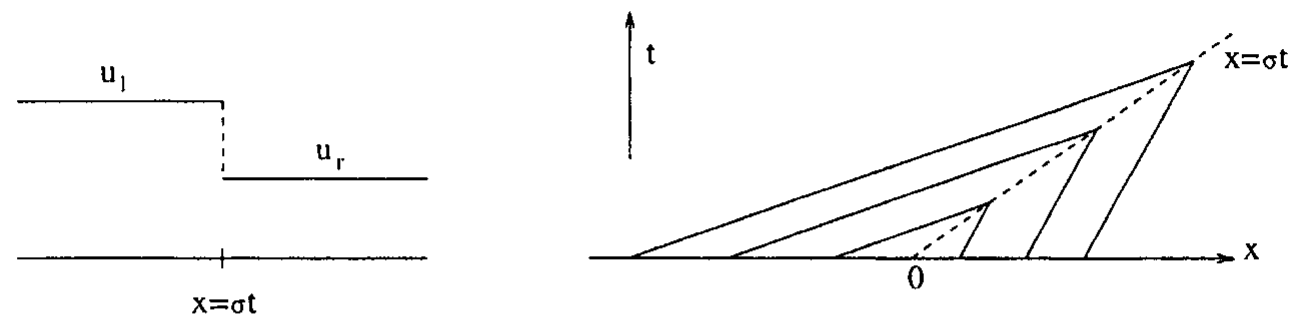
\includegraphics[width=.710\paperwidth]{images/fig-14-1-1.png}
  \caption{Riemann 问题的激波解(熵解)}\label{fig:14.1.1}
\end{figure}
\[
  \begin{aligned}
    0&=\frac{d}{dt}(u_l+u_r)
     =\frac{d}{dt}\biggl[\int_{\sigma t-1}^{\sigma t}u(t,x)\,\mathrm dx
                        +\int_{\sigma t}^{\sigma t+1}u(t,x)\,\mathrm dx\biggr]\\
     &=\int_{\sigma t-1}^{\sigma t+1}\frac{\partial u}{\partial t}(t,x)\,\mathrm dx
                      -\sigma(u_l-u_r),
  \end{aligned}
\]
从而
\begin{equation}\label{eq:14.1.30}
  \sigma(u_l-u_r)=F(u_l)-F(u_r).
\end{equation}
这个关系对任意通量函数 \(F\) 都成立.对于 Burgers 方程,\(F(u)=u^2/2\),故 \(\sigma\) 取\eqref{eq:14.1.28}的形式.

关系\eqref{eq:14.1.30}称为 \emph{Rankine--Hugoniot 跳跃条件}.在更一般的情形下,任一激波的两侧都满足这个条件.此时,\(u_l\) 和 \(u_r\) 分别表示解在间断处的左值和右值,\(\sigma\) 则是相应的瞬时速度.

当 \(u_l<u_r\) 时,有无穷多个弱解.其中一个仍是\eqref{eq:14.1.27},见\figref{fig:14.1.2},但此时特征线从间断向外发出.可以证明这个解不稳定：数据的微小扰动会导致解发生显著变化.
\begin{figure}[htbp]
  \centering
  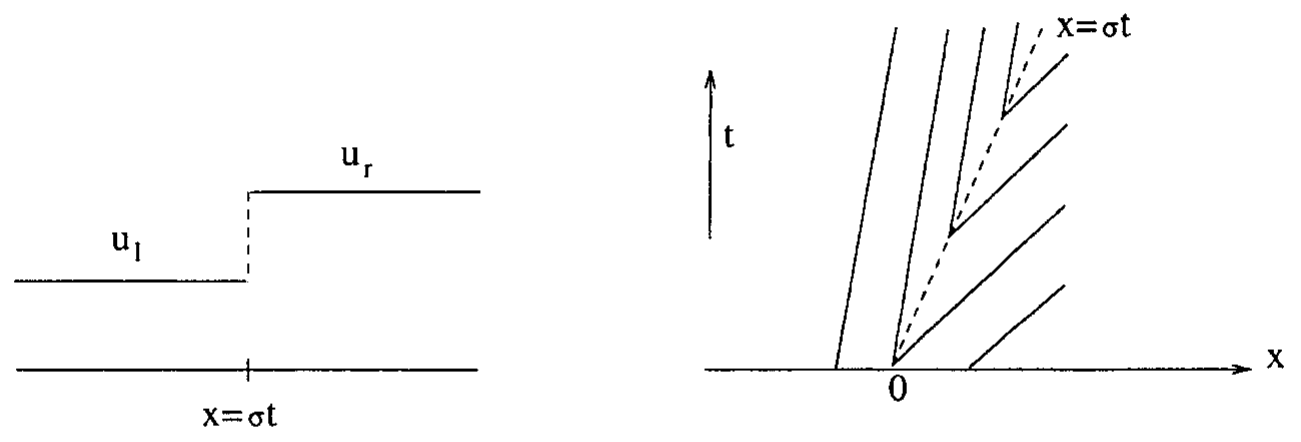
\includegraphics[width=.710\paperwidth]{images/fig-14-1-2.png}
  \caption{Riemann 问题中违反熵条件的解}\label{fig:14.1.2}
\end{figure}
另一个在扰动下稳定的弱解是
\SourcePage{467}
\begin{equation}\label{eq:14.1.31}
  u(t,x)=\begin{cases}
    u_l, & x<u_lt,\\
    x/t, & u_lt\le x\le u_rt,\\
    u_r, & x>u_rt.
  \end{cases}
\end{equation}
这就是 Burgers 方程的消失黏性解,也就是熵解,见\figref{fig:14.1.3}.
\end{example}

前面的讨论说明了如何构造熵条件.如上所见,时间向前推进时,激波两侧的特征线应当进入间断.如果特征线从间断向外发出,那么初始数据或方程本身的微小扰动,例如加入少量黏性,都可能使解发生很大变化,典型结果是形成特征线的稀疏扇.

因此可得如下判据.传播速度 \(\sigma\) 由\eqref{eq:14.1.30}给出的间断,在下列条件下满足熵条件：
\begin{equation}\label{eq:14.1.32}
  F'(u_l)>\sigma>F'(u_r).
\end{equation}
当 \(F\) 严格凸时,Rankine--Hugoniot 条件\eqref{eq:14.1.30}表明,\(\sigma\) 必介于 \(F'(u_l)\) 与 \(F'(u_r)\) 之间.所以\eqref{eq:14.1.32}只要求 \(F'(u_l)>F'(u_r)\),根据严格凸性,这等价于 \(u_l>u_r\).

当 \(F\) 非凸时,可采用下面更一般的判据.传播速度 \(\sigma\) 由\eqref{eq:14.1.30}给出的间断,若对所有介于 \(u_l\) 和 \(u_r\) 之间的 \(u\) 都有
\begin{equation}\label{eq:14.1.33}
  \frac{F(u)-F(u_l)}{u-u_l}\ge\sigma
       \ge\frac{F(u)-F(u_r)}{u-u_r},
\end{equation}
则满足熵条件.

熵条件的另一种表述使用熵函数与熵通量.从守恒律\eqref{eq:14.1.20}出发,假定对光滑解 \(u\),有一对函数 \(\eta(u)\) 和 \(\mu(u)\) 满足
\begin{equation}\label{eq:14.1.34}
  \frac{\partial}{\partial t}\eta(u)+\frac{\partial}{\partial x}\mu(u)=0.
\end{equation}
\begin{definition*}
函数 \(\eta(u)\) 和 \(\mu(u)\) 分别称为{\heiti 熵函数}和{\heiti 熵通量}.
\end{definition*}
函数 \(\eta\)、\(\mu\) 与 \(F\) 的关系为
\begin{equation}\label{eq:14.1.35}
  \mu'(u)=\eta'(u)F'(u).
\end{equation}
事实上,设 \(u\) 光滑,由\eqref{eq:14.1.34}有
\[
  \eta'(u)\frac{\partial u}{\partial t}
        +\mu'(u)\frac{\partial u}{\partial x}=0,
\]
而由\eqref{eq:14.1.20},
\SourcePage{468}
\begin{figure}[htbp]
  \centering
  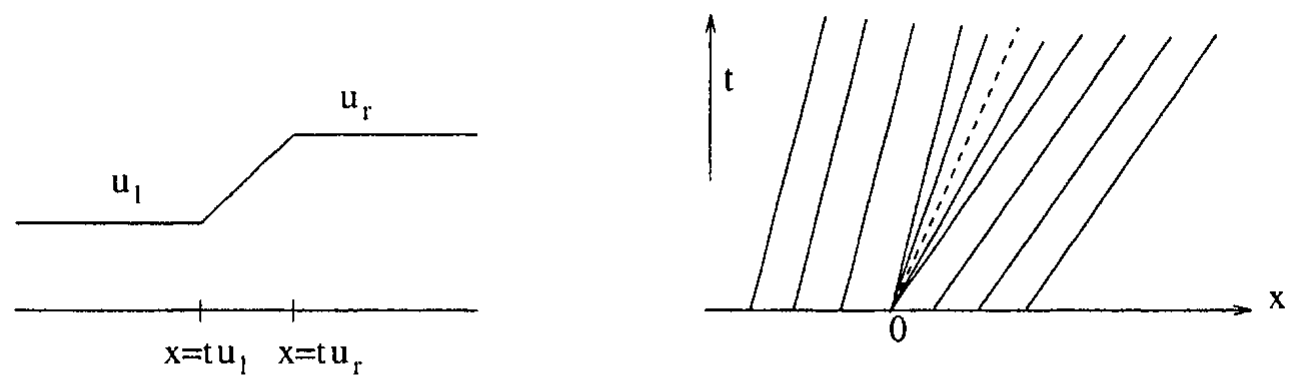
\includegraphics[width=.709\paperwidth]{images/fig-14-1-3.png}
  \caption{Riemann 问题的稀疏波解(熵解)}\label{fig:14.1.3}
\end{figure}
\[
  0=\eta'(u)\biggl[\frac{\partial u}{\partial t}
                      +F'(u)\frac{\partial u}{\partial x}\biggr].
\]
比较两式即得\eqref{eq:14.1.35}.

熵条件的第三种表述如下.
\begin{definition*}
如果对所有凸熵函数 \(\eta(\cdot)\) 及对应的熵通量 \(\mu(\cdot)\),熵不等式
\begin{equation}\label{eq:14.1.36}
  \frac{\partial}{\partial t}\eta(u)+\frac{\partial}{\partial x}\mu(u)\le0
\end{equation}
均在弱意义下成立,那么称弱解 \(u(t,x)\) 为\eqref{eq:14.1.20}的{\heiti 熵解}.
\end{definition*}

可以用下面的启发式推导解释这一条件.利用\eqref{eq:14.1.25}和\eqref{eq:14.1.35},得到
\[
  \begin{aligned}
    \frac{\partial}{\partial t}\eta(u^\varepsilon)
        +\frac{\partial}{\partial x}\mu(u^\varepsilon)
      &=\eta'(u^\varepsilon)\biggl[
            \frac{\partial u^\varepsilon}{\partial t}
              +F'(u^\varepsilon)\frac{\partial u^\varepsilon}{\partial x}\biggr]
       =\varepsilon\eta'(u^\varepsilon)\frac{\partial^2u^\varepsilon}{\partial x^2}\\
      &=\varepsilon\biggl[
          \frac{\partial}{\partial x}\biggl(\eta'(u^\varepsilon)
                  \frac{\partial u^\varepsilon}{\partial x}\biggr)
          -\eta''(u^\varepsilon)\biggl(\frac{\partial u^\varepsilon}{\partial x}\biggr)^2\biggr]\\
      &\le\varepsilon\frac{\partial}{\partial x}\biggl(
                      \eta'(u^\varepsilon)\frac{\partial u^\varepsilon}{\partial x}\biggr).
  \end{aligned}
\]
令 \(\varepsilon\to0\) 并取 \(u:=\lim_{\varepsilon\to0}u^\varepsilon\),形式上即得\eqref{eq:14.1.36}.

\eqref{eq:14.1.36}的弱形式是
\begin{equation}\label{eq:14.1.37}
  \begin{aligned}
    &-\int_0^\infty\!\!\int_{-\infty}^\infty
     \biggl[\eta(u(t,x))\frac{\partial\varphi}{\partial t}(t,x)
           +\mu(u(t,x))\frac{\partial\varphi}{\partial x}(t,x)\biggr]
                   \,\mathrm dx\,\mathrm dt\\
    &\qquad\le\int_{-\infty}^\infty\varphi(0,x)\eta(u(0,x))\,\mathrm dx,
  \end{aligned}
\end{equation}
其中 \(\varphi\) 可取 \(C_0^1([0,\infty)\times\mathbb R)\) 中的任一函数,只要对所有 \((t,x)\in[0,\infty)\times\mathbb R\) 有 \(\varphi(t,x)\ge0\).

对于 \(F(u)=u^2/2\) 的 Burgers 方程,例如取 \(\eta(u)=u^2\),由\eqref{eq:14.1.35}得 \(\mu'(u)=2u^2\),故可取 \(\mu(u)=2u^3/3\).熵不等式\eqref{eq:14.1.36}成为
\begin{equation}\label{eq:14.1.38}
  \frac{\partial}{\partial t}u^2+\frac{\partial}{\partial x}\biggl(\frac23u^3\biggr)\le0.
\end{equation}
\SourcePage{469}
对于光滑解,等号成立.当出现间断时,可以证明\eqref{eq:14.1.38}成立当且仅当 \((u_l-u_r)^3>0\),即如所预期的 \(u_l>u_r\).对于给定的数值方法,可以用\eqref{eq:14.1.36}的离散形式检验数值解是否收敛到熵解.

综上,物理解 \(u=\lim_{\varepsilon\to0}u^\varepsilon\) 是\eqref{eq:14.1.20}的一类弱解,满足熵条件\eqref{eq:14.1.36}.\BookCite{kruzkov1970}{Kruzkov(1970)}证明,熵解存在,并由初始数据 \(u_0(x)\) 唯一确定.

关于非线性守恒律的深入分析,可参阅\BookCite{courant-friedrichs1948}{Courant 和 Friedrichs(1948)}、\BookCite{oleinik1957}{Oleinik(1957)}、\BookCite{lax1973}{Lax(1973)}和\BookCite{smoller1983}{Smoller(1983)}等.

\section{有限差分逼近}\label{sec:14.2}

为作基于有限差分的时空逼近,选取时间步长 \(\Delta t\) 和网格宽度 \(\Delta x\),以网格点 \((t_n,x_j)\) 离散 \((t,x)\) 平面,其中
\[
  t_n:=n\Delta t,\quad n=0,1,\ldots,\qquad
  x_j:=j\Delta x,\quad j\in\mathbb Z.
\]
定义网格比 \(\lambda:=\Delta t/\Delta x\),并记 \(x_{j+1/2}:=x_j+\Delta x/2\).我们要寻找对所有 \(j,n\) 逼近 \(u(t_n,x_j)\) 的离散解 \(u_j^n\).有时 \(u_j^n\) 用来逼近所谓的\emph{单元平均值}
\[
  \overline u_j^n:=\frac1{\Delta x}
    \int_{x_{j-1/2}}^{x_{j+1/2}}u(t_n,x)\,\mathrm dx.
\]
有限体积法经常采用后一种做法.

\subsection{线性标量对流方程与双曲型方程组}\label{sec:14.2.1}

双曲型初值问题一般用显式方法作时间推进,因而通常要限制网格比 \(\lambda\) 才能保持稳定性.隐式方法一般没有这一限制.\tabref{tab:14.2.1}列出了对 \(a\) 为常数的线性对流方程\eqref{eq:14.1.1}的几种格式.除蛙跳格式外,表中的方法都是两层格式,只涉及时间层 \(t_n\) 和 \(t_{n+1}\).

有些方法采用中心有限差分,即在逼近节点 \(x_j\) 处的 \(x\) 导数时,同时使用 \(u_{j-1}\) 和 \(u_{j+1}\).\emph{中心向前 Euler 法}是其中最简单的一个例子,见\tabref{tab:14.2.1}.可惜它不稳定,稳定性的定义见下一小节.Lax--Friedrichs 法是 Euler 法的一个小改动,仅把 \(u_j^n\) 换成 \(u_{j+1}^n\) 和
\SourcePage{470}
\(u_{j-1}^n\) 的平均值,从而获得更好的稳定性,见第~\BookRef{sec:14.2.2}{14.2.2}~节.另一些方法采用单边有限差分,迎风法和 Warming--Beam 法就属于这一类.

\begin{table}[htbp]
  \centering
  \caption{问题\eqref{eq:14.1.1}的显式有限差分格式}\label{tab:14.2.1}
  \small
  \setlength{\tabcolsep}{4pt}
  \renewcommand{\arraystretch}{1.45}
  \begin{tabular}{@{}lll@{}}
    \toprule
    格式 & 差分方程 & \shortstack[l]{数值通量函数\\\(h_{j+1/2}\)}\\
    \midrule
    \shortstack[l]{中心向前\\Euler}
      & \(u_j^{n+1}=u_j^n-\tfrac{\lambda}{2}a(u_{j+1}^n-u_{j-1}^n)\)
      & \(\tfrac12a(u_{j+1}+u_j)\)\\
    迎风
      & \(\begin{aligned}[t]
          u_j^{n+1}&=u_j^n-\tfrac{\lambda}{2}a(u_{j+1}^n-u_{j-1}^n)\\
            &\quad+\tfrac{\lambda}{2}|a|(u_{j+1}^n-2u_j^n+u_{j-1}^n)
         \end{aligned}\)
      & \(\begin{aligned}[t]
          &\tfrac12[a(u_{j+1}+u_j)\\
          &\qquad-|a|(u_{j+1}-u_j)]
        \end{aligned}\)\\
    \shortstack[l]{Lax--\\Friedrichs}
      & \(\begin{aligned}[t]
          u_j^{n+1}&=\tfrac12(u_{j+1}^n+u_{j-1}^n)\\
            &\quad-\tfrac{\lambda}{2}a(u_{j+1}^n-u_{j-1}^n)
         \end{aligned}\)
      & \(\begin{aligned}[t]
          &\tfrac12[a(u_{j+1}+u_j)\\
          &\qquad-\tfrac1\lambda(u_{j+1}-u_j)]
        \end{aligned}\)\\
    \shortstack[l]{Lax--\\Wendroff}
      & \(\begin{aligned}[t]
          u_j^{n+1}&=u_j^n-\tfrac{\lambda}{2}a(u_{j+1}^n-u_{j-1}^n)\\
            &\quad+\tfrac{\lambda^2}{2}a^2(u_{j+1}^n-2u_j^n+u_{j-1}^n)
         \end{aligned}\)
      & \(\begin{aligned}[t]
          &\tfrac12[a(u_{j+1}+u_j)\\
          &\qquad-\lambda a^2(u_{j+1}-u_j)]
        \end{aligned}\)\\
    \shortstack[l]{Warming--\\Beam (\(a>0\))}
      & \(\begin{aligned}[t]
          u_j^{n+1}&=u_j^n-\tfrac{\lambda}{2}a(3u_j^n-4u_{j-1}^n+u_{j-2}^n)\\
            &\quad+\tfrac{\lambda^2}{2}a^2(u_j^n-2u_{j-1}^n+u_{j-2}^n)
         \end{aligned}\)
      & \(\begin{aligned}[t]
          &\tfrac12[a(3u_j-u_{j-1})\\
          &\qquad-\lambda a^2(u_j-u_{j-1})]
        \end{aligned}\)\\
    蛙跳 & \(u_j^{n+1}=u_j^{n-1}-\lambda a(u_{j+1}^n-u_{j-1}^n)\) & \\
    \bottomrule
  \end{tabular}
\end{table}

\emph{迎风法}的推导如下.
\SourcePage{471}
\begin{equation}\label{eq:14.2.1}
  \frac{u_j^{n+1}-u_j^n}{\Delta t}
    =\begin{cases}
       -\dfrac{a}{\Delta x}(u_{j+1}^n-u_j^n), & a<0,\\[4pt]
       -\dfrac{a}{\Delta x}(u_j^n-u_{j-1}^n), & a>0.
     \end{cases}
\end{equation}
等价地,可写为
\begin{equation}\label{eq:14.2.2}
  \frac{u_j^{n+1}-u_j^n}{\Delta t}
    +a\frac{u_{j+1}^n-u_{j-1}^n}{2\Delta x}
    =\tfrac12|a|\Delta x
         \frac{u_{j+1}^n-2u_j^n+u_{j-1}^n}{(\Delta x)^2}.
\end{equation}
与中心向前 Euler 法相比,\eqref{eq:14.2.2}的右端增加了一项
\begin{equation}\label{eq:14.2.3}
  \varepsilon\frac{u_{j+1}^n-2u_j^n+u_{j-1}^n}{(\Delta x)^2},
\end{equation}
其中 \(\varepsilon=\tfrac12|a|\Delta x\).因为 \((u_{j+1}-2u_j+u_{j-1})/(\Delta x)^2\) 是 \(x_j\) 处 \(\partial^2u/\partial x^2\) 的一个逼近,\eqref{eq:14.2.3}就是为稳定格式而加入的\emph{人工黏性}项,也称\emph{数值耗散}项.

\emph{Lax--Wendroff 法}从关于 \(t=t_n\) 的二阶 Taylor 展开出发,而无须直接对\eqref{eq:14.1.1}中的时空导数作有限差分逼近：
\[
  \begin{aligned}
    u(t_{n+1},x_j)
      &=u(t_n,x_j)+\Delta t\frac{\partial u}{\partial t}(t_n,x_j)\\
      &\qquad+\tfrac12(\Delta t)^2\frac{\partial^2u}{\partial t^2}(t_n,x_j)
                +O((\Delta t)^3).
  \end{aligned}
\]
利用\eqref{eq:14.1.1}可得
\[
  \frac{\partial u}{\partial t}=-a\frac{\partial u}{\partial x},
  \qquad \frac{\partial^2u}{\partial t^2}=a^2\frac{\partial^2u}{\partial x^2}.
\]
将这两式代入,保留 Taylor 展开右端的前三项,再用中心有限差分逼近空间导数,就得到 Lax--Wendroff 法.

\emph{Warming--Beam 法}的推导类似,不过空间导数采用单边差分逼近.\tabref{tab:14.2.1}给出的是 \(a>0\) 时的公式.

容易看出,Lax--Friedrichs 法引入的数值耗散仍具有\eqref{eq:14.2.3}的形式,其中 \(\varepsilon=(\Delta x)^2/(2\Delta t)\).Lax--Wendroff 法中对应的系数为 \(\varepsilon=\tfrac12a^2\Delta t\).

分别在模板 \((j-1,j,j+1)\) 和 \((j-2,j-1,j)\) 上,Lax--Wendroff 格式和 Warming--Beam 格式是唯一具有二阶精度的两层格式.参见\BookCite{hirsch1988}{Hirsch(1988,第 357–360 页)}.若把它们视为下列修正\emph{色散}方程的直接逼近,两种方法实际上都具有三阶精度：
\[
  \frac{\partial u}{\partial t}+a\frac{\partial u}{\partial x}
    =\varepsilon\frac{\partial^3u}{\partial x^3}.
\]
\SourcePage{472}
具体而言,Lax--Wendroff 格式的色散系数为 \(\varepsilon=\tfrac{(\Delta x)^2}{6}a(\lambda^2a^2-1)\),Warming--Beam 格式的为 \(\varepsilon=\tfrac{(\Delta x)^2}{6}a(2-3\lambda a+\lambda^2a^2)\).关于色散波理论,\BookCite{whitham1974}{Whitham(1974)}有详尽论述.

\tabref{tab:14.2.1}中的两层显式有限差分法都可写成统一形式
\begin{equation}\label{eq:14.2.4}
  u_j^{n+1}=u_j^n-\lambda(h_{j+1/2}^n-h_{j-1/2}^n),
\end{equation}
其中通常取 \(h_{j+1/2}=h(u_j,u_{j+1})\),Warming--Beam 法在 \(a>0\) 时则取 \(h_{j+1/2}=h(u_{j-1},u_j)\).函数 \(h(\cdot,\cdot)\) 称为\emph{数值通量函数},各方法的具体表达式见\tabref{tab:14.2.1}.

简洁形式\eqref{eq:14.2.4}的优点是便于推广到更一般的双曲型问题,尤其是线性方程组和非线性方程.考虑方程组\eqref{eq:14.1.6}时,仍可按\tabref{tab:14.2.1}作有限差分逼近,只须留意记号的变化.首先,把 \(a\) 换成矩阵 \(A\),把 \(a^2\) 换成 \(A^2\),并以逼近 \(\boldsymbol{U}(t_n,x_j)\) 的向量 \(\boldsymbol{U}_j^n\) 代替 \(u_j^n\).此外,在迎风法中,应以
\begin{equation}\label{eq:14.2.5}
  |A|:=T|\Lambda|T^{-1}
\end{equation}
代替 \(|a|\),其中 \(|\Lambda|:=\operatorname{diag}(|\lambda_1|,\ldots,|\lambda_p|)\),见\eqref{eq:14.1.7}.

这一公式的来由很容易理解.先将方程组\eqref{eq:14.1.6}变换为 \(p\) 个独立的对流方程\eqref{eq:14.1.9},再对其中每个方程应用标量迎风格式.这样得到
\[
  \begin{aligned}
    (W_k)_j^{n+1}&=(W_k)_j^n-\tfrac{\lambda}{2}\lambda_k
                       [(W_k)_{j+1}^n-(W_k)_{j-1}^n]\\
        &\qquad+\tfrac{\lambda}{2}|\lambda_k|
                  [(W_k)_{j+1}^n-2(W_k)_j^n+(W_k)_{j-1}^n],
  \end{aligned}
\]
其中 \(k=1,\ldots,p\).用紧凑记号写为
\[
  \boldsymbol{W}_j^{n+1}=\boldsymbol{W}_j^n-\tfrac{\lambda}{2}\Lambda(\boldsymbol{W}_{j+1}^n-\boldsymbol{W}_{j-1}^n)
     +\tfrac{\lambda}{2}|\Lambda|(\boldsymbol{W}_{j+1}^n-2\boldsymbol{W}_j^n+\boldsymbol{W}_{j-1}^n).
\]
通过变换 \(T\boldsymbol{W}_j^n=\boldsymbol{U}_j^n\) 回到物理变量 \(\boldsymbol{U}_j^n\),便得到向量迎风法
\begin{equation}\label{eq:14.2.6}
  \begin{aligned}
    \boldsymbol{U}_j^{n+1}
      &=\boldsymbol{U}_j^n-\tfrac{\lambda}{2}A(\boldsymbol{U}_{j+1}^n-\boldsymbol{U}_{j-1}^n)\\
      &\qquad+\tfrac{\lambda}{2}|A|(\boldsymbol{U}_{j+1}^n-2\boldsymbol{U}_j^n+\boldsymbol{U}_{j-1}^n).
  \end{aligned}
\end{equation}
向量情形下,上述两层时间推进格式也可改写为
\begin{equation}\label{eq:14.2.7}
  \boldsymbol{U}_j^{n+1}=\boldsymbol{U}_j^n
       -\lambda(\boldsymbol{H}_{j+1/2}^n-\boldsymbol{H}_{j-1/2}^n),
\end{equation}
\SourcePage{473}
其中 \(\boldsymbol{H}_{j+1/2}\) 为\emph{数值通量向量函数}.它的表达式很容易由标量情形推广得到,即分别用 \(A\)、\(A^2\)、\(|A|\) 代替 \(a\)、\(a^2\)、\(|a|\).

\subsection{稳定性、相容性与收敛性}\label{sec:14.2.2}

任意两层方法都可写成紧凑形式
\begin{equation}\label{eq:14.2.8}
  \boldsymbol{u}^{n+1}=E_{\Delta t}(\boldsymbol{u}^n),
\end{equation}
其中 \(\boldsymbol{u}^n\) 表示 \(t_n\) 时刻的近似值向量 \(\{u_j^n\mid j\in\mathbb Z\}\).按分量写为
\begin{equation}\label{eq:14.2.9}
  u_j^{n+1}=E_{\Delta t}(\boldsymbol{u}^n;j).
\end{equation}
例如,中心向前 Euler 法的算子 \(E_{\Delta t}\) 取形式
\begin{equation}\label{eq:14.2.10}
  E_{\Delta t}(\boldsymbol{u}^n;j)=u_j^n-\tfrac{\lambda a}{2}(u_{j+1}^n-u_{j-1}^n).
\end{equation}

\begin{definition*}
如果对任意 \(T>0\),均存在常数 \(C_T>0\)(可依赖于 \(T\))和 \(\delta_0>0\),使得对所有满足 \(n\Delta t\le T\)、\(0<\Delta t\le\delta_0\)、\(0<\Delta x\le\delta_0\) 的允许网格和时间层,都有
\begin{equation}\label{eq:14.2.11}
  \|\boldsymbol{u}^n\|_\Delta\le C_T\|\boldsymbol{u}^0\|_\Delta,
\end{equation}
则称该方法在 Lax--Richtmyer 意义下{\heiti 稳定}.这里
\begin{equation}\label{eq:14.2.12}
  \|\boldsymbol{v}\|_\Delta:=\Delta x\sum_{j=-\infty}^{\infty}|v_j|
\end{equation}
是 \(L^1(\mathbb R)\) 范数的离散近似,见\eqref{eq:14.1.5}.
\end{definition*}
由于 \(\boldsymbol{u}^n=E_{\Delta t}^n(\boldsymbol{u}^0)\),只要存在 \(\beta\ge0\),使得对每个允许的 \(0<\Delta t\le\delta_0\)、\(0<\Delta x\le\delta_0\),都有
\[
  \|E_{\Delta t}\boldsymbol{v}\|_\Delta
      \le(1+\beta\Delta t)\|\boldsymbol{v}\|_\Delta\qquad\forall\boldsymbol{v},
\]
稳定性便成立.事实上,当 \(n\Delta t\le T\) 时,
\[
  \|\boldsymbol{u}^n\|_\Delta\le(1+\beta\Delta t)^n\|\boldsymbol{u}^0\|_\Delta
       \le e^{\beta T}\|\boldsymbol{u}^0\|_\Delta,
\]
从而得到\eqref{eq:14.2.11}.

现在讨论相容性.定义\emph{局部截断误差}为
\[
  (\mathcal T_{\Delta t}(t))_j
     :=\frac1{\Delta t}[u(t+\Delta t,x_j)-E_{\Delta t}(u(t);j)],
\]
其中 \(E_{\Delta t}(u(t);j)\) 随所用的两层方法而定,其定义是在\eqref{eq:14.2.9}右端用 \(u(t,x_j)\) 代替 \(u_j^n\).
\SourcePage{474}
\begin{definition*}
若沿所选网格族,随着 \(\Delta t,\Delta x\to0\),对所有 \(t>0\) 都有
\begin{equation}\label{eq:14.2.13}
  \lim_{\Delta t,\Delta x\to0}\|\mathcal T_{\Delta t}(t)\|_\Delta=0,
\end{equation}
则称两层方法{\heiti 相容}.进一步,如果对所有足够光滑的初始数据,都有某个常数 \(C>0\),使得
\begin{equation}\label{eq:14.2.14}
  \|\mathcal T_{\Delta t}(t)\|_\Delta\le C[(\Delta t)^{q_1}+(\Delta x)^{q_2}],
    \qquad t>0
\end{equation}
对所有允许的 \(0<\Delta t\le\delta_0\)、\(0<\Delta x\le\delta_0\) 成立,就称该方法在时间上为 \(q_1\) 阶,在空间上为 \(q_2\) 阶.
\end{definition*}
离散时,\(\Delta t\) 和 \(\Delta x\) 常成正比,即对某个正常数 \(\kappa\) 有 \(\Delta t=\kappa\Delta x\).此时称方法为 \(q\) 阶,其中 \(q=\min(q_1,q_2)\).还应指出,当用方法\eqref{eq:14.2.8}逼近定常解时,起决定作用的是空间阶,也就是 \(\Delta x\) 的指数 \(q_2\).

\begin{definition*}
如果当 \(\Delta t,\Delta x\to0\) 时有
\[
  \max_{0\le n\le T/\Delta t}\|u(t_n,\cdot)-\boldsymbol{u}^n\|_\Delta\to0,
\]
则称该格式{\heiti 收敛}.
\end{definition*}

线性双曲型初值问题理论的基本结果是 Lax--Richtmyer 等价定理.
\begin{theorem*}
对适定的线性初值问题,相容的线性差分方法收敛的充要条件是稳定性.
\end{theorem*}
Lax--Richtmyer 等价定理的证明见\BookCite{richtmyer-morton1967}{Richtmyer 和 Morton(1967)},另见\BookCite{strikwerda1989}{Strikwerda(1989)}.

下面说明几个稳定性结果.例如,对 Lax--Friedrichs 法,有
\[
  \|\boldsymbol{u}^{n+1}\|_\Delta=\Delta x\sum_j|u_j^{n+1}|
     \le\frac{\Delta x}{2}
       \biggl[\sum_j|(1-\lambda a)u_{j+1}^n|
                     +\sum_j|(1+\lambda a)u_{j-1}^n|\biggr].
\]
假定
\begin{equation}\label{eq:14.2.15}
  |a\lambda|=\biggl|a\frac{\Delta t}{\Delta x}\biggr|\le1,
\end{equation}
则 \(1-\lambda a\) 和 \(1+\lambda a\) 都非负,因而
\[
  \begin{aligned}
    \|\boldsymbol{u}^{n+1}\|_\Delta
       &\le\frac{\Delta x}{2}\biggl[(1-a\lambda)\sum_j|u_{j+1}^n|
                        +(1+a\lambda)\sum_j|u_{j-1}^n|\biggr]\\
       &\le\tfrac12(1-a\lambda)\|\boldsymbol{u}^n\|_\Delta
             +\tfrac12(1+a\lambda)\|\boldsymbol{u}^n\|_\Delta=\|\boldsymbol{u}^n\|_\Delta.
  \end{aligned}
\]
因此,只要满足稳定性限制\eqref{eq:14.2.15},\eqref{eq:14.2.11}便以 \(C_T=1\) 成立.

类似地,只要 \(\Delta t\) 和 \(\Delta x\) 满足\eqref{eq:14.2.15},就可证明迎风法稳定.事实上,当 \(a>0\) 时,迎风格式\eqref{eq:14.2.1}为
\SourcePage{475}
\[
  u_j^{n+1}=u_j^n-\lambda a(u_j^n-u_{j-1}^n).
\]
于是
\[
  \|\boldsymbol{u}^{n+1}\|_\Delta\le\Delta x\sum_j|(1-\lambda a)u_j^n|
                            +\Delta x\sum_j|\lambda a u_{j-1}^n|.
\]
若\eqref{eq:14.2.15}成立,则 \(u_j^n\) 和 \(u_{j-1}^n\) 的系数均非负,故 \(\|\boldsymbol{u}^{n+1}\|_\Delta\le\|\boldsymbol{u}^n\|_\Delta\).\(a<0\) 时也得到同样的结果.

中心向前 Euler 法在类似\eqref{eq:14.2.15}的限制下会失稳.不过,在离散 \(L^2\) 范数下,取 \(\Delta t=O((\Delta x)^2)\) 可使它稳定.参见\BookCite{strikwerda1989}{Strikwerda(1989,第 49 页)}.

将\eqref{eq:14.2.15}中的不等号改为严格不等号,并使 \(|\lambda a|\) 一致小于 \(1\),也足以保证蛙跳格式在离散 \(L^2\) 范数下稳定.事实上,用 \(u_j^{n+1}+u_j^{n-1}\) 乘蛙跳方程并求和,得
\[
  \begin{aligned}
    &\sum_j[(u_j^{n+1})^2+\lambda a(u_j^{n+1}u_{j+1}^n-u_{j-1}^n u_j^{n+1})]\\
    &\quad=\sum_j[(u_j^{n-1})^2+\lambda a(u_{j-1}^n u_j^{n-1}-u_j^{n-1}u_{j+1}^n)].
  \end{aligned}
\]
在两端各加上 \(\sum_j(u_j^n)^2\),并注意对每个 \(k\ge0\),由移项求和有
\[
  \sum_i u_{i-1}^k u_i^{k+1}
    =\sum_i\bigl[u_i^k u_{i+1}^{k+1}
        -(u_i^k u_{i+1}^{k+1}-u_{i-1}^k u_i^{k+1})\bigr]
    =\sum_i u_i^k u_{i+1}^{k+1},
\]
就可从上一等式得到
\[
  \sum_j G_j^{n+1}=\sum_j G_j^n,
\]
其中
\[
  G_j^n:=(u_j^n)^2+(u_j^{n-1})^2
          +a\lambda(u_j^n u_{j+1}^{n-1}-u_{j+1}^n u_j^{n-1}).
\]
因此,\(\sum_j G_j^{n+1}=\sum_j G_j^1\),即
\[
  \begin{aligned}
    &\sum_j[(u_j^{n+1})^2+(u_j^n)^2+\lambda a(u_j^{n+1}u_{j+1}^n-u_{j+1}^{n+1}u_j^n)]\\
    &\quad=\sum_j[(u_j^1)^2+(u_j^0)^2+\lambda a(u_j^1u_{j+1}^0-u_{j+1}^1u_j^0)].
  \end{aligned}
\]
利用不等式 \(-x^2-y^2\le2xy\le x^2+y^2\),可得
\[
  (1-|\lambda a|)\sum_j[(u_j^{n+1})^2+(u_j^n)^2]
     \le(1+|\lambda a|)\sum_j[(u_j^1)^2+(u_j^0)^2].
\]
设 \(|\lambda a|\le c<1\),其中 \(c\) 固定.因此,对每个 \(T\),存在常数 \(C_T>0\),使得所有满足 \(n\Delta t\le T\) 的 \(n\) 均有
\SourcePage{476}
\[
  \|\boldsymbol{u}^n\|_{2,\Delta}
    \le C_T(\|\boldsymbol{u}^0\|_{2,\Delta}^2+\|\boldsymbol{u}^1\|_{2,\Delta}^2)^{1/2},
  \qquad
  \|\boldsymbol{v}\|_{2,\Delta}:=\biggl(\Delta x\sum_j|v_j|^2\biggr)^{1/2}.
\]
这一稳定性不等式在离散 \(L^2\) 范数下将\eqref{eq:14.2.11}推广到三层有限差分格式.

用类似方法可以证明,Lax--Wendroff 法在相同的限制\eqref{eq:14.2.15}下也是稳定的,范数仍取离散 \(L^2\) 范数.

另一种证明稳定性的方法是 von Neumann 分析,它对有限差分方程作 Fourier 变换.这种方法在\BookCite{richtmyer-morton1967}{Richtmyer 和 Morton(1967)}和\BookCite{strikwerda1989}{Strikwerda(1989)}中有详尽讨论,另见\BookCite{vichnevetsky-bowles1982}{Vichnevetsky 和 Bowles(1982)}.Warming--Beam 格式的一个基于 von Neumann 分析的稳定性证明,见\BookCite{hirsch1988}{Hirsch(1988,第 9.3 节)}.其稳定性条件是 \(|a\lambda|\le2\),对 \(\lambda\) 的限制比\eqref{eq:14.2.15}宽松.原因在于,\emph{差分模板}是把计算 \(u_j^{n+1}\) 涉及的所有网格点连接起来的图.Warming--Beam 格式的模板在 \(x_j\) 的一侧用了两个点.

更确切地说,稳定性条件可作如下几何解释.对于具有 Lax--Wendroff 型模板的有限差分格式,\(u_j^{n+1}\) 依赖于上一时间层在 \(x_{j+i}\)(\(i=-1,0,1\))三个点的值.一直回溯到 \(t=0\),可见 \(u_j^{n+1}\) 只依赖于 \(i=-(n+1),\ldots,n+1\) 对应的 \(x_{j+i}\) 处的初始数据.因此,\(u_j^n\) 的\emph{数值依赖域} \(D_{\Delta t}(t_n,x_j)\) 满足
\[
  D_{\Delta t}(t_n,x_j)\subset
    \bigl\{x\in\mathbb R\mid |x-x_j|\le n\Delta x=t_n/\lambda\bigr\}.
\]
对任一固定点 \((\bar t,\bar x)\),相应地有
\[
  D_{\Delta t}(\bar t,\bar x)\subset
    \bigl\{x\in\mathbb R\mid |x-\bar x|\le\bar t/\lambda\bigr\}.
\]
特别地,保持 \(\lambda\) 固定并令 \(\Delta t\to0\),极限数值依赖域为
\[
  D_0(\bar t,\bar x)=\bigl\{x\in\mathbb R\mid |x-\bar x|\le\bar t/\lambda\bigr\}.
\]
条件\eqref{eq:14.2.15}等价于
\begin{equation}\label{eq:14.2.16}
  D(\bar t,\bar x)\subset D_0(\bar t,\bar x),
\end{equation}
其中 \(D(\bar t,\bar x)\) 是\eqref{eq:14.1.11}定义的依赖域.由于现在考虑标量情形,这里 \(p=1\)、\(\lambda_1=a\).

对于一致格式,这个条件是稳定性的必要条件.事实上,若不满足它,精确依赖域中就存在某个点 \(y^*\),
\SourcePage{477}
不属于数值依赖域.改变 \(y^*\) 附近的初始数据会改变精确解,却不会改变数值解,因而无法收敛.根据 Lax--Richtmyer 等价定理,这也排除了稳定性.

\begin{definition*}
\eqref{eq:14.2.15}称为 {\heiti CFL 条件}.\BookCite{courant-friedrichs-lewy1928}{Courant、Friedrichs 和 Lewy(1928)}证明,这是数值解稳定的一个必要条件.特别地,对双曲型初值问题,任何采用固定有限模板的显式相容有限差分格式都要受这一类稳定性限制.
\end{definition*}
在上面的一些例子中,CFL 条件既是数值格式稳定的必要条件,也是充分条件.不过,也有方法在满足 CFL 条件时仍不稳定.

向量情形也有类似的稳定性条件.例如,将 Lax--Wendroff 型模板用于\eqref{eq:14.1.6}时,步长须满足
\begin{equation}\label{eq:14.2.17}
  \biggl|\lambda_k\frac{\Delta t}{\Delta x}\biggr|\le1,\qquad k=1,\ldots,p,
\end{equation}
其中 \(\{\lambda_k\mid k=1,\ldots,p\}\) 是 \(A\) 的特征值.这些条件也可写成\eqref{eq:14.2.16}的形式.换言之,每条直线 \(x=\bar x-\lambda_k(\bar t-t)\) 与时间层 \(t=\bar t-\Delta t\) 的交点 \(x^{(k)}\) 都必须落在差分模板的底边上,见\figref{fig:14.2.1}.

\begin{figure}[htbp]
  \centering
  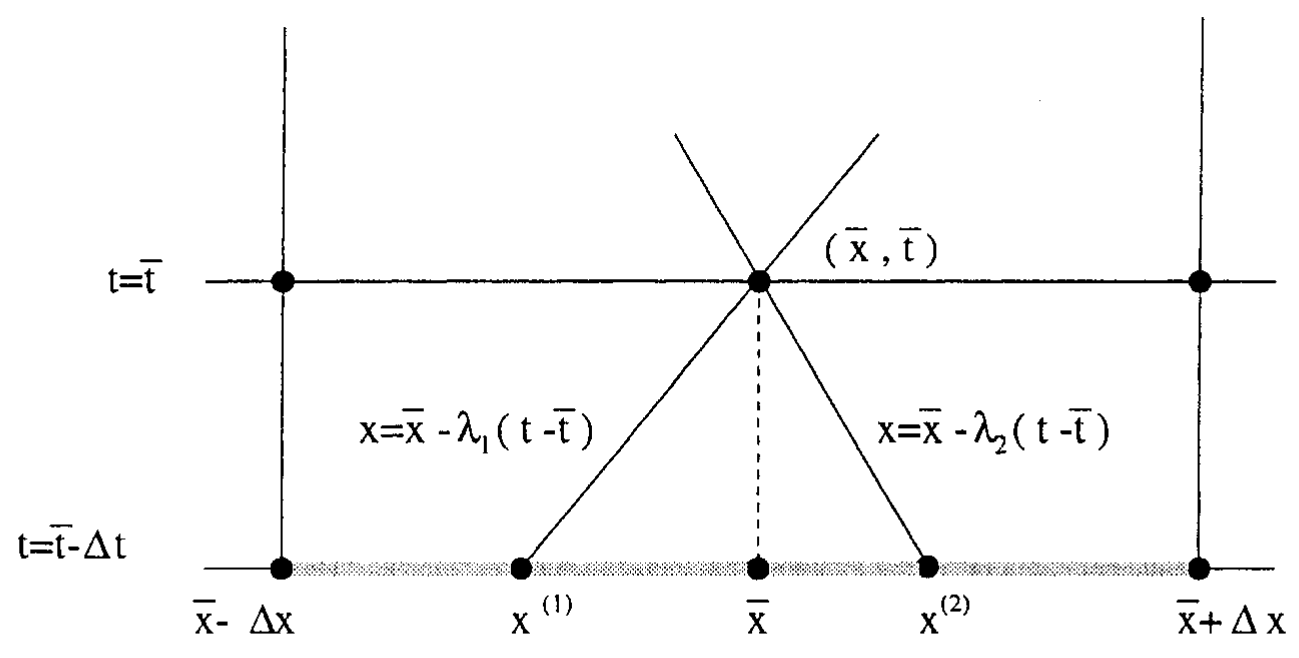
\includegraphics[width=.709\paperwidth]{images/fig-14-2-1.png}
  \caption{CFL 条件\eqref{eq:14.2.17}的几何解释}\label{fig:14.2.1}
\end{figure}

\begin{note}
\NumberedNote{note:14.2.1}{\heiti(边界处理)}考虑 \(a>0\) 时的下列初边值问题：
\SourcePage{478}
\[
  \begin{cases}
    \dfrac{\partial u}{\partial t}+a\dfrac{\partial u}{\partial x}=0,
        & t>0,\quad 0<x<1,\\[2pt]
    u(t,0)=\varphi_-(t), & t>0,\\
    u(0,x)=u_0(x), & 0<x<1.
  \end{cases}
\]
选定正整数 \(M\) 后,令 \(\Delta x:=1/M\),\(x_j:=j\Delta x\),\(j=0,\ldots,M\).

有限差分格式在每个内部点 \(x_j\)(\(j=1,\ldots,M-1\))离散微分方程,并在流入点施加给定的边界条件.许多有限差分格式还须添加边界条件才能唯一确定数值解,这些附加条件通常称为{\heiti 数值边界条件}.例如,采用 Lax--Wendroff 法或 Lax--Friedrichs 法时,格式无法直接用于流出点 \(x_M\),因为它需要计算区间 \([0,1]\) 外的 \(x_{M+1}\) 处的 \(u_{M+1}^n\).一般用外推公式求出 \(u_M^{n+1}\),外推可有多种形式.例如,可取 \(u_M^{n+1}=u_{M-1}^{n+1}\)(常值外推),或取 \(u_M^{n+1}=2u_{M-1}^{n+1}-u_{M-2}^{n+1}\)(线性外推),还可取 \(u_M^{n+1}=2u_{M-1}^n-u_{M-2}^{n-1}\)(沿特征线的近似线性外推).

还可用单边差分格式导出数值边界条件.例如,对 Lax--Wendroff 法,可以用
\[
  u_M^{n+1}=u_M^n-\lambda a(u_M^n-u_{M-1}^n).
\]
这是在流出点 \((t_{n+1},x_M)\) 应用 Lax--Wendroff 格式,并用线性外推公式 \(u_{M+1}^n=2u_M^n-u_{M-1}^n\) 计算 \(u_{M+1}^n\) 得到的.

需要强调,数值边界条件有时会使原本对纯初值问题稳定的有限差分格式失稳.例如,对蛙跳格式,常值外推和线性外推均不稳定,沿特征线外推则稳定.对隐式 Crank--Nicolson 格式,上述结论正好相反.

关于数值边界条件的详尽分析,见\BookCite{strikwerda1989}{Strikwerda(1989,第 11 章)}.\hfill\(\square\)
\end{note}

\subsection{非线性标量方程}\label{sec:14.2.3}
\SourcePage{479}

考虑非线性标量守恒律
\begin{equation}\label{eq:14.2.18}
  \begin{cases}
    \dfrac{\partial u}{\partial t}+\dfrac{\partial}{\partial x}F(u)=0,
       &t>0,\quad x\in\mathbb R,\\[2pt]
    u(0,x)=u_0(x), &x\in\mathbb R,
  \end{cases}
\end{equation}
并以 \(a(u):=F'(u)\) 表示特征速度.

这里着重考虑间断解.对于光滑解,第~\ref{sec:14.2}~节已介绍的方法通常可以有效地用于线性化方程.不过,从第~\ref{sec:14.1.4}~节已经知道,即使初始数据光滑,也很容易产生间断解.间断解的数值逼近很有挑战性,至今仍是一个活跃的研究领域.本小节只介绍几个基本概念,并举例说明一些激波捕捉格式.系统介绍可参阅\BookCite{yee1989}{Yee(1989)}、\BookCite{leveque1990}{LeVeque(1990)}、\BookCite{godlewski-raviart1991}{Godlewski 和 Raviart(1991)}及其中的参考文献.

与线性情形一样,\emph{守恒形式}的三点显式有限差分格式一般按如下原则构造：
\begin{equation}\label{eq:14.2.19}
  u_j^{n+1}=u_j^n-\lambda(h_{j+1/2}^n-h_{j-1/2}^n),
\end{equation}
其中仍有 \(h_{j+1/2}^n:=h(u_j^n,u_{j+1}^n)\),\(h(\cdot,\cdot)\) 为\emph{数值通量函数}.最一般的情形可写成
\[
  u_j^{n+1}=u_j^n-\lambda[H(u_{j-p}^n,\ldots,u_{j+q}^n)
                              -H(u_{j-p-1}^n,\ldots,u_{j+q-1}^n)],
\]
其中 \(H\) 是一个有 \(p+q+1\) 个变量的函数,\(p,q\ge0\).

下面用一个推导说明\eqref{eq:14.2.19}的由来.由\eqref{eq:14.2.18}得
\[
  \begin{aligned}
    \int_{x_{j-1/2}}^{x_{j+1/2}}u(t_{n+1},x)\,\mathrm dx
      &=\int_{x_{j-1/2}}^{x_{j+1/2}}u(t_n,x)\,\mathrm dx\\
      &\quad-\biggl[\int_{t_n}^{t_{n+1}}F(u(t,x_{j+1/2}))\,\mathrm dt
                -\int_{t_n}^{t_{n+1}}F(u(t,x_{j-1/2}))\,\mathrm dt\biggr].
  \end{aligned}
\]
两端除以 \(\Delta x\),并用本节开头定义的单元平均值 \(\overline u_j^n\),得到
\[
  \overline u_j^{n+1}=\overline u_j^n
    -\frac1{\Delta x}\biggl[\int_{t_n}^{t_{n+1}}F(u(t,x_{j+1/2}))\,\mathrm dt
                   -\int_{t_n}^{t_{n+1}}F(u(t,x_{j-1/2}))\,\mathrm dt\biggr].
\]
与\eqref{eq:14.2.19}比较可知
\[
  h_{j+1/2}^n\simeq\frac1{\Delta t}\int_{t_n}^{t_{n+1}}
                    F(u(t,x_{j+1/2}))\,\mathrm dt,
\]
\SourcePage{480}
即数值通量函数相当于时间区间 \([t_n,t_{n+1}]\) 内通过 \(x_{j+1/2}\) 的平均通量.

为与守恒律\emph{相容},要求数值通量函数在常值解情形下化为真实通量 \(F\),即
\begin{equation}\label{eq:14.2.20}
  h(\overline u_0,\overline u_0)=F(\overline u_0),
     \qquad u(t,x)\equiv\overline u_0.
\end{equation}
此外,还要求 \(h\) 对每个变量都是 Lipschitz 连续的.

如第~\ref{sec:14.2.2}~节所见,线性问题的稳定性分析已经相当成熟.然而,线性化方程的局部稳定性对于非线性问题的稳定性既非必要条件,也非充分条件,尤其是在有强间断时.数值方法可能对线性化问题稳定,却在非线性问题上失稳,这称为\emph{非线性不稳定}.

加入线性数值耗散,也称人工黏性,是常用的稳定化手段,在计算流体力学中尤为普遍.在非线性情形下,单靠这一手段,既无法保证收敛到物理上正确的熵解,也无法保证收敛到弱解.这里可用\BookCite{lax-wendroff1960}{Lax 和 Wendroff(1960)}的定理.
\begin{theorem*}
如果有限差分格式采用守恒形式,与给定的守恒律相容,并且其数值解有满足定理所需收敛性和有界性条件的极限,则该极限是守恒律的弱解.
\end{theorem*}
这样得到的弱解未必满足熵条件.事实上,确有守恒且相容的数值方法收敛到违反熵条件的弱解.

第~\ref{sec:14.1}~节已经说明,只给定初始值,弱解一般无法唯一确定,还须施加熵条件.在有限维层面,也需要用离散熵条件选出符合物理的解.仿照\eqref{eq:14.1.36},离散熵不等式可以写成
\[
  \eta(u_j^{n+1})\le\eta(u_j^n)
        -\lambda[\mu_\Delta(\boldsymbol{u}^n;j)-\mu_\Delta(\boldsymbol{u}^n;j-1)].
\]
式中的 \(\mu_\Delta\) 是某个离散熵通量函数.它应与 \(\mu\) 相容,正如数值通量函数 \(h_{j+1/2}\) 须与 \(F\) 相容一样.

现在回顾几个定义.先把\eqref{eq:14.2.19}改写为
\begin{equation}\label{eq:14.2.21}
  u_j^{n+1}=G(u_{j-1}^n,u_j^n,u_{j+1}^n).
\end{equation}
\begin{definition*}
如果 \(G\) 关于它的每个变量都是单调不减的,就称该数值格式为{\heiti 单调格式}.
\end{definition*}
对单个守恒律,固定 \(\Delta t/\Delta x\),当 \(\Delta t\to0\) 时,用相容且守恒的单调格式得到的数值解总是收敛到符合物理的解.证明见\BookCite{harten-hyman-lax1976}{Harten、Hyman 和 Lax(1976)}或\BookCite{crandall-majda1980}{Crandall 和 Majda(1980)}.

\SourcePage{481}
\begin{definition*}
若存在 \(C>0\),使得
\[
  \sup_{j,n}|u_j^n|\le C,
\]
则称数值格式\eqref{eq:14.2.21}为{\heiti 有界}.
\end{definition*}
\begin{definition*}
若从两个不同的初值 \(\boldsymbol{u}^0\) 和 \(\boldsymbol{v}^0\) 出发得到的有限差分解 \(\boldsymbol{u}^n,\boldsymbol{v}^n\) 满足
\[
  \|\boldsymbol{u}^n-\boldsymbol{v}^n\|_\Delta
     \le C_T\|\boldsymbol{u}^0-\boldsymbol{v}^0\|_\Delta
\]
对所有 \(0\le n\Delta t\le T\) 成立,其中 \(C_T>0\),\(\|\cdot\|_\Delta\) 由\eqref{eq:14.2.12}定义,则称格式{\heiti 稳定}.对线性问题,这一定义等价于\eqref{eq:14.2.11}.
\end{definition*}

\BookCite{kuznetsov1976}{Kuznetsov(1976)}证明,单调守恒格式有界、稳定,收敛到熵解,且精度至多为一阶.另见\BookCite{harten-hyman-lax1976}{Harten、Hyman 和 Lax(1976)}.这类格式在间断附近给出平滑过渡.

下面给出几种数值通量函数的实例.它们通过\eqref{eq:14.2.19}导出若干熟知的有限差分格式.

\begin{example}[Lax--Friedrichs 格式]\label{ex:14.2.lf}
为简便起见,记 \(F_j:=F(u_j)\).\emph{Lax--Friedrichs 格式}对应于取
\begin{equation}\label{eq:14.2.22}
  h_{j+1/2}=\tfrac12\bigl[F_{j+1}+F_j-\tfrac1\lambda(u_{j+1}-u_j)\bigr],
\end{equation}
因而写成
\begin{equation}\label{eq:14.2.23}
  u_j^{n+1}=\tfrac12(u_{j+1}^n+u_{j-1}^n)
              -\tfrac{\lambda}{2}\bigl(F(u_{j+1}^n)-F(u_{j-1}^n)\bigr).
\end{equation}
可以证明,这个方法在固定网格比下是相容的,并具有一阶精度.若在解的取值区间内满足 CFL 条件
\[
  \biggl|F'(v)\frac{\Delta t}{\Delta x}\biggr|\le1,
\]
则该方法在此区间上单调.
\end{example}

\begin{example}[Lax--Wendroff 格式]\label{ex:14.2.lw}
\emph{Lax--Wendroff 法}对应的数值通量是
\begin{equation}\label{eq:14.2.24}
  h_{j+1/2}=\tfrac12[F_{j+1}+F_j-\lambda a_{j+1/2}(F_{j+1}-F_j)],
\end{equation}
因而格式为
\begin{equation}\label{eq:14.2.25}
  \begin{aligned}
    u_j^{n+1}
      &=u_j^n-\tfrac{\lambda}{2}\bigl(F(u_{j+1}^n)-F(u_{j-1}^n)\bigr)\\
      &\quad+\tfrac{\lambda^2}{2}\bigl[a_{j+1/2}^n(F(u_{j+1}^n)-F(u_j^n))
                 -a_{j-1/2}^n(F(u_j^n)-F(u_{j-1}^n))\bigr].
  \end{aligned}
\end{equation}
这里令
\[
  a_{j+1/2}:=F'\bigl((u_{j+1}+u_j)/2\bigr).
\]
\SourcePage{482}
该方法在光滑解上具有二阶精度,但不单调.它还需要计算 Jacob 矩阵 \(F'(\cdot)\),对方程组来说,这项工作可能并不容易.下列 Lax--Wendroff 改进格式仍具有二阶精度,仍为守恒格式,并省去了 \(F'(\cdot)\) 的计算：
\begin{equation}\label{eq:14.2.26}
  \begin{aligned}
    u_{j+1/2}^{n+1/2}
       &=\tfrac12(u_{j+1}^n+u_j^n)-\tfrac{\lambda}{2}[F(u_{j+1}^n)-F(u_j^n)],\\
    u_j^{n+1}
       &=u_j^n-\lambda[F(u_{j+1/2}^{n+1/2})-F(u_{j-1/2}^{n+1/2})].
  \end{aligned}
\end{equation}
其数值通量为
\begin{equation}\label{eq:14.2.27}
  h_{j+1/2}=F\bigl(\tfrac12(u_{j+1}+u_j)-\tfrac{\lambda}{2}(F_{j+1}-F_j)\bigr).
\end{equation}
\end{example}

\begin{example}[MacCormack 格式]\label{ex:14.2.maccormack}
另一种做法是 \emph{MacCormack 法},它先用向前差分,再用向后差分：
\begin{equation}\label{eq:14.2.28}
  \begin{aligned}
    u_j^*&=u_j^n-\lambda[F(u_{j+1}^n)-F(u_j^n)],\\
    u_j^{n+1}&=\tfrac12(u_j^n+u_j^*)-\tfrac{\lambda}{2}[F(u_j^*)-F(u_{j-1}^*)].
  \end{aligned}
\end{equation}
该格式具有二阶精度,且为守恒格式.因此,若它收敛到含激波的解,激波满足正确的跳跃条件.格式本身没有为间断处专门加入耗散.对于线性标量对流方程,它化为 Lax--Wendroff 法.数值通量为
\begin{equation}\label{eq:14.2.29}
  h_{j+1/2}=\tfrac12F_{j+1}+\tfrac12F(u_j-\lambda(F_{j+1}-F_j)).
\end{equation}
\end{example}

\begin{example}[Courant--Isaacson--Rees 格式]\label{ex:14.2.cir}
对于线性标量对流方程,\emph{Courant--Isaacson--Rees 法}化为迎风法.对于非线性问题\eqref{eq:14.2.18},由于 \(u\) 沿光滑解的特征线保持常值,可以在 \(x_j-F'(u_j^n)\Delta t\) 处用数据 \(\boldsymbol{u}^n\) 作线性插值,以此逼近 \(u_j^{n+1}\).若 \(F'(u_j^n)>0\),格式为
\[
  u_j^{n+1}=u_j^n-\lambda F'(u_j^n)(u_j^n-u_{j-1}^n).
\]
一般可写为
\begin{equation}\label{eq:14.2.30}
  \begin{aligned}
    u_j^{n+1}=u_j^n-\lambda\biggl[
      &\frac{|F'(u_j^n)|+F'(u_j^n)}{2}(u_j^n-u_{j-1}^n)\\
      &+\frac{F'(u_j^n)-|F'(u_j^n)|}{2}(u_{j+1}^n-u_j^n)\biggr].
  \end{aligned}
\end{equation}
由于这一方法缺少守恒形式,用它来逼近激波并不合适.
\end{example}

\begin{example}[Godunov 格式]\label{ex:14.2.godunov}
\emph{Godunov 法}既利用特征信息,也保持守恒形式.其做法是从每个界面出发,沿时间正向求解 Riemann 问题.沿特征线回溯的做法已在上一例题中介绍.
\SourcePage{483}
具体来说,给定 \(n\),用离散解 \(\boldsymbol{u}^n\) 定义分片常值函数 \(v^n(x)\),使它在整个区间 \(x_{j-1/2}<x<x_{j+1/2}\) 上取值 \(u_j^n\).然后以 \(v^n(x)\) 作为时刻 \(t_n\) 的初值,在 \((t_n,t_{n+1})\) 上求解守恒律.若 \(\Delta t\) 足够小,方程实际上可以通过一系列 Riemann 问题精确求解.\(\Delta t\) 须满足类似 CFL 的条件,以避免相邻 Riemann 问题相互影响.在 \([t_n,t_{n+1}]\times\mathbb R\) 上,只需将这些 Riemann 问题的解拼接起来,便得到 \(u_*^n(t,x)\).最后,通过对 \(u_*^n\) 取平均来定义新时间层 \(t_{n+1}\) 的离散解 \(\boldsymbol{u}^{n+1}\)：
\[
  u_j^{n+1}:=\frac1{\Delta x}\int_{x_{j-1/2}}^{x_{j+1/2}}
                    u_*^n(t_{n+1},x)\,\mathrm dx.
\]
根据这些值再构造新的分片常值函数 \(v^{n+1}(x)\),重复上述过程.

所得格式可以写成守恒形式\eqref{eq:14.2.19},其中数值通量为
\begin{equation}\label{eq:14.2.31}
  h_{j+1/2}^n=\frac1{\Delta t}\int_{t_n}^{t_{n+1}}
                 F(u_*^n(t,x_{j+1/2}))\,\mathrm dt.
\end{equation}
这一格式是单调迎风格式,并满足熵条件.还可以证明,数值通量函数为
\[
  h_{j+1/2}=
  \begin{cases}
    \min\{F(u)\mid u_j\le u\le u_{j+1}\}, & u_j\le u_{j+1},\\
    \max\{F(u)\mid u_{j+1}\le u\le u_j\}, & u_j>u_{j+1}.
  \end{cases}
\]
对于线性问题,Godunov 格式化为迎风格式.
\end{example}

\begin{example}[Engquist--Osher 格式]\label{ex:14.2.engquist-osher}
还有一种采用守恒形式的单调迎风法,即 \emph{Engquist--Osher 格式}.它对应的数值通量函数为
\begin{equation}\label{eq:14.2.32}
  h_{j+1/2}=F_j+F_{j+1}^--F_j^-=F_{j+1}-F_{j+1}^++F_j^+,
\end{equation}
其中
\[
  F_j^+:=F(\max(u_j,\overline u)),\qquad
  F_j^-:=F(\min(u_j,\overline u)),
\]
\(\overline u\) 是严格凸通量 \(F(u)\) 的声速点,即满足 \(F'(\overline u)=0\) 的值.
\end{example}

\subsection{高阶激波捕捉格式}\label{sec:14.2.4}

单调的一阶迎风格式耗散过强.对于复杂流场,要得到准确的解,就需要非常细的网格.为减少数值耗散,应采用高阶激波捕捉格式.
\SourcePage{484}
当然,为了得到无振荡的激波并保证收敛到熵解,仍需要一定的耗散.

高阶方法(例如至少二阶)的基本思想是,从一个原本可以达到高阶精度的方法出发,在间断附近加入数值耗散作修正.附加项可模拟与 \(\partial^2u/\partial x^2\) 成正比的扩散项,有时也用 \(\partial^4u/\partial x^4\).其系数记为 \(\varepsilon\).当 \(\Delta t,\Delta x\to0\) 时,\(\varepsilon\) 必须足够快地趋于零,使格式既与双曲型方程相容,又能在光滑解上保持高阶精度.

这类格式有两种.经典方法采用\emph{线性}数值耗散,也就是各点使用同样的耗散.例如 Lax--Wendroff、MacCormack 和 Warming--Beam 法.

现代方法采用\emph{非线性}数值耗散.这意味着扩散系数 \(\varepsilon\) 取决于解本身的性质,在间断附近比在光滑区域大.这类做法可在空间上达到二阶、三阶甚至更高的精度.其设计原则如下：
\begin{enumerate}[label=\alph*.]
  \item 采用守恒形式,以保证捕捉激波的能力.
  \item 在间断附近避免非物理的过冲和振荡,同时清晰分辨激波.
  \item 在流动的光滑区域达到高精度.
  \item 使极限解满足熵条件.
\end{enumerate}
传统方法,例如 Lax--Wendroff 型格式,通常无法满足第 b 项和第 d 项.

这些格式首先针对一维非线性标量方程构造.借助 Riemann 求解器(精确或近似)或通量向量分裂技术,可以推广到方程组.

这里不深入分析这类方法,只说明主要概念并给出几个例子.

回顾一下,光滑函数 \(u\colon\mathbb R\to\mathbb R\) 的\emph{总变差}可定义为下列积分,在有界变差的情形下该值有限：
\[
  \operatorname{TV}(u):=\int_{-\infty}^{\infty}|u'(x)|\,\mathrm dx.
\]
若 \(\boldsymbol{u}^n\) 是一个网格函数,则其总变差可定义为
\begin{equation}\label{eq:14.2.33}
  \operatorname{TV}(\boldsymbol{u}^n):=\sum_j|u_{j+1}^n-u_j^n|.
\end{equation}
\begin{definition*}
如果一个差分方法对每个时间层 \(n\ge0\) 和允许的 \(\Delta t>0\) 都满足
\begin{equation}\label{eq:14.2.34}
  \operatorname{TV}(\boldsymbol{u}^{n+1})\le\operatorname{TV}(\boldsymbol{u}^n),
\end{equation}
则称该方法具有{\heiti 总变差递减性},简称 TVD.
\end{definition*}

\SourcePage{485}
即使一个 TVD 格式具有守恒形式且与守恒律相容,它也未必与熵不等式一致.

标量守恒律的单调格式具有 TVD 性质,证明见\BookCite{crandall-majda1980}{Crandall 和 Majda(1980)}.

一族采用守恒形式的\emph{五点}差分格式可写为
\begin{equation}\label{eq:14.2.35}
  u_j^{n+1}+\theta\lambda(h_{j+1/2}^{n+1}-h_{j-1/2}^{n+1})
    =u_j^n-(1-\theta)\lambda(h_{j+1/2}^n-h_{j-1/2}^n),
\end{equation}
其中 \(h_{j+1/2}\) 表示数值通量函数,在这里取形式
\[
  h_{j+1/2}=h(u_{j-1},u_j,u_{j+1},u_{j+2}).
\]
仍有 \(\lambda:=\Delta t/\Delta x\),\(0\le\theta\le1\) 是一个参数.\(\theta=0\) 时格式为显式,\(\theta>0\) 时为隐式.

将\eqref{eq:14.2.35}改写为
\[
  L(\boldsymbol{u}^{n+1})=R(\boldsymbol{u}^n),
\]
其中 \(L\) 和 \(R\) 是有限差分算子：
\[
  \begin{aligned}
    L(\boldsymbol{u})_j&:=u_j+\theta\lambda(h_{j+1/2}-h_{j-1/2}),\\
    R(\boldsymbol{u})_j&:=u_j-(1-\theta)\lambda(h_{j+1/2}-h_{j-1/2}).
  \end{aligned}
\]
\BookCite{harten1984}{Harten(1984)}指出,\eqref{eq:14.2.35}具有 TVD 性质的充分条件为
\[
  \operatorname{TV}(R(\boldsymbol{u}^n))\le\operatorname{TV}(\boldsymbol{u}^n),\qquad
  \operatorname{TV}(L(\boldsymbol{u}^{n+1}))\ge\operatorname{TV}(\boldsymbol{u}^{n+1}).
\]
定义新的通量
\begin{equation}\label{eq:14.2.36}
  \overline h_{j+1/2}^n:=(1-\theta)h_{j+1/2}^n+\theta h_{j+1/2}^{n+1}.
\end{equation}
于是,对适当的通量函数 \(\overline h\),有
\[
  \overline h_{j+1/2}^n
    =\overline h(u_{j-1}^n,u_j^n,u_{j+1}^n,u_{j+2}^n,
                u_{j-1}^{n+1},u_j^{n+1},u_{j+1}^{n+1},u_{j+2}^{n+1}).
\]
只要函数 \(\overline h\) 满足
\begin{equation}\label{eq:14.2.37}
  \overline h(\underbrace{u,u,\ldots,u}_{8\text{ 个}})=F(u),
\end{equation}
就与\eqref{eq:14.1.20}相容.这时,\eqref{eq:14.2.35}变为
\begin{equation}\label{eq:14.2.38}
  u_j^{n+1}=u_j^n-\lambda(\overline h_{j+1/2}^n-\overline h_{j-1/2}^n),
\end{equation}
它与线性标量方程的\eqref{eq:14.2.4}类似.

\begin{example}[Roe 迎风通量]\label{ex:14.2.roe}
作为 TVD 格式的一个例子,定义
\[
  \widetilde a_{j+1/2}:=\frac{F_{j+1}-F_j}{u_{j+1}-u_j},
\]
相邻状态相等时取 \(\widetilde a_{j+1/2}=F'(u_j)\).对形如
\SourcePage{486}
\begin{equation}\label{eq:14.2.39}
  h_{j+1/2}=\tfrac12[F_{j+1}+F_j-|\widetilde a_{j+1/2}|(u_{j+1}-u_j)]
\end{equation}
的数值通量函数,即一阶 Roe 迎风通量,TVD 性质的一个充分条件是下列 CFL 型条件：
\[
  |\lambda\widetilde a_{j+1/2}|\le\frac1{1-\theta}\qquad(0\le\theta<1).
\]
\(\theta=1\) 时此条件不限制步长.参见\BookCite{harten1984}{Harten(1984)}.
\end{example}

现在讨论高阶 TVD 格式的设计原则.多数高阶 TVD 格式可看作带有适当数值耗散或光滑机制的中心差分格式.这里有一个反馈机制,能够自动调节数值耗散的大小.线性理论中使用的耗散则预先给定.

一般而言,给定与格式\eqref{eq:14.2.19}对应的高阶通量函数 \(h(\boldsymbol{u};j)\),加入人工耗散相当于用修改后的通量函数
\begin{equation}\label{eq:14.2.40}
  h^{\rm art}(\boldsymbol{u};j):=h(\boldsymbol{u};j)
             -\Delta x\,\varepsilon(\boldsymbol{u};j)(u_{j+1}-u_j)
\end{equation}
代替原通量.有时也采用比\eqref{eq:14.2.40}更一般的形式
\[
  h^{\rm art}(\boldsymbol{u};j):=h(\boldsymbol{u};j)+\Phi(\boldsymbol{u};j).
\]
若基准通量为中心通量,所得数值通量可写成
\[
  h_{j+1/2}=\tfrac12(F_{j+1}+F_j+\Phi_{j+1/2}).
\]
换言之,\(h_{j+1/2}\) 是二阶中心格式的通量与人工耗散之和,人工耗散在这里起 TVD 修正的作用.

困难在于怎样选取适当的 \(\varepsilon(\cdot;\cdot)\) 或 \(\Phi(\cdot;\cdot)\),使耗散足以保持单调性,同时又能保持精度.

这一要求不易满足,因此实际中往往采用更直接的做法.具体来说,高阶格式主要借助称为\emph{限制器}的限制程序来满足 TVD 的充分条件.这些程序约束因变量 \(u\) 的梯度,称为\emph{斜率限制器},或者约束通量函数 \(F\),称为\emph{通量限制器}.对常系数问题,两类限制器等价.

注意,任一高阶通量 \(h^{\rm high}\) 一般可以写成低阶通量 \(h^{\rm low}\) 加上一个修正,即
\[
  h^{\rm high}(\boldsymbol{u};j)
    =h^{\rm low}(\boldsymbol{u};j)+[h^{\rm high}(\boldsymbol{u};j)-h^{\rm low}(\boldsymbol{u};j)].
\]
典型的通量限制器方法对应于形如
\begin{equation}\label{eq:14.2.41}
  h^{\rm lim}(\boldsymbol{u};j)=h^{\rm low}(\boldsymbol{u};j)
     +\Phi(\boldsymbol{u};j)[h^{\rm high}(\boldsymbol{u};j)-h^{\rm low}(\boldsymbol{u};j)]
\end{equation}
的通量.修正项通常称为\emph{反扩散通量},因为它补偿了低阶通量引入的较多数值扩散.
\SourcePage{487}
\BookCite{boris-book1973}{Boris 和 Book(1973)}的\emph{通量修正输运法}(FCT)就基于这一思想,是最早的高分辨率方法之一.

一种常见做法是取 \(\Phi(\boldsymbol{u};j)=\varphi(\theta_j)\),其中 \(\theta_j:=(u_j-u_{j-1})/(u_{j+1}-u_j)\).两个例子是\BookCite{roe1985}{Roe(1985)}的 superbee 限制器,其函数为 \(\varphi(\theta):=\max(0,\min(1,2\theta),\min(\theta,2))\),以及\BookCite{van-leer1974}{van Leer(1974)}的限制器 \(\varphi(\theta):=(\theta+|\theta|)/(1+|\theta|)\).

可以证明,TVD 格式在解的局部极值点处退化为一阶精度.实际上,只有在解单调的地方,才能达到 TVD 格式的形式精度.因此,所说的 TVD 格式空间精度,是指远离激波且单调区域内的数值解精度.

TVD 格式可分为\emph{迎风} TVD 格式和\emph{对称}(或\emph{中心})TVD 格式.“迎风”和“对称”指应用限制器之前的格式.前者的耗散项采用迎风加权,后者的耗散项采用对称加权.通常,对称格式的耗散略大,但所需运算量比迎风 TVD 格式少.

\begin{example}[MUSCL 格式]\label{ex:14.2.muscl}
一种很常用的 TVD 格式是 \emph{MUSCL},即守恒律的单调迎风中心格式,由\BookCite{van-leer1979}{van Leer(1979)}提出.它的思想是在 Godunov 格式中,用分片线性重构代替 Riemann 问题的分片常值初始数据,从而达到空间二阶精度.

同样的做法显然也可从其他类型的数值通量函数出发.例如,考虑二阶 Roe 数值通量
\begin{equation}\label{eq:14.2.42}
  \begin{aligned}
    h_{j+1/2}
      &=\tfrac12\Bigl[F(u_{j+1/2}^R)+F(u_{j+1/2}^L)\\
      &\qquad-\biggl|\frac{F(u_{j+1/2}^R)-F(u_{j+1/2}^L)}
                          {u_{j+1/2}^R-u_{j+1/2}^L}\biggr|
                    (u_{j+1/2}^R-u_{j+1/2}^L)\Bigr].
  \end{aligned}
\end{equation}
对这一通量应用 MUSCL 方法,采用如下定义的 \(u_{j+1/2}^R\) 和 \(u_{j+1/2}^L\)：
\[
  \begin{aligned}
    u_{j+1/2}^R&:=u_{j+1}
      -\tfrac14[(1-\eta)\Delta_{j+3/2}u+(1+\eta)\Delta_{j+1/2}u],\\
    u_{j+1/2}^L&:=u_j
      +\tfrac14[(1-\eta)\Delta_{j-1/2}u+(1+\eta)\Delta_{j+1/2}u],
  \end{aligned}
\]
其中
\[
  \Delta_{j+1/2}u:=u_{j+1}-u_j.
\]
\(\eta\) 的值决定空间精度.几个例子是 \(\eta=-1\)(全迎风格式)、\(\eta=0\)(Fromm 格式)、\(\eta=1/3\)(三阶偏迎风格式,之所以称为偏迎风,是因为模板中有一个下游点)和 \(\eta=1\)(三点中心差分格式).

\SourcePage{488}
可以用多种斜率限制器消除多余的振荡.具体做法是取
\[
  \begin{aligned}
    u_{j+1/2}^R&:=u_{j+1}
      -\tfrac14[(1-\eta)\Delta^*_{j+3/2}u+(1+\eta)\Delta^{**}_{j+1/2}u],\\
    u_{j+1/2}^L&:=u_j
      +\tfrac14[(1-\eta)\Delta^{**}_{j-1/2}u+(1+\eta)\Delta^*_{j+1/2}u],
  \end{aligned}
\]
其中 \(\Delta^*\) 和 \(\Delta^{**}\) 是适当的算子.例如,\emph{minmod} 限制器定义为
\[
  \begin{aligned}
    \Delta^*_{j+1/2}u&:=\operatorname{minmod}(\Delta_{j+1/2}u,\omega\Delta_{j-1/2}u),\\
    \Delta^{**}_{j+1/2}u&:=\operatorname{minmod}(\Delta_{j+1/2}u,\omega\Delta_{j+3/2}u),
  \end{aligned}
\]
这里
\[
  \operatorname{minmod}(x,\omega y)
    :=\operatorname{sign}(x)\max\{0,\min[|x|,\omega y\operatorname{sign}(x)]\},
\]
且 \(1\le\omega\le(3-\eta)/(1-\eta)\),\(-1\le\eta<1\).这个格式可简写为
\begin{equation}\label{eq:14.2.43}
  u_j^{n+1}=u_j^n-\lambda\bigl[
     h(u_{j+1/2}^{R,n},u_{j+1/2}^{L,n})-h(u_{j-1/2}^{R,n},u_{j-1/2}^{L,n})\bigr],
\end{equation}
注意它与\eqref{eq:14.2.4}在形式上相似,正如\eqref{eq:14.2.39}和\eqref{eq:14.2.42}在形式上相似.
\end{example}

其他 MUSCL 型 TVD 格式见\BookCite{harten1984}{Harten(1984)}、\BookCite{roe1985}{Roe(1985)}、\BookCite{sweby1984}{Sweby(1984)}以及\BookCite{osher-chakravarthy1986}{Osher 和 Chakravarthy(1986)},另见\BookCite{osher1985}{Osher(1985)}.MUSCL 以外的 TVD 格式则有\BookCite{davis1984}{Davis(1984)}、\BookCite{roe1984}{Roe(1984)}和\BookCite{yee1987}{Yee(1987)}的方法.

较新的发展包括 TVB 和 ENO 格式.
\begin{definition*}
如果存在 \(B=B(\boldsymbol{u}^0)>0\),使得对所有满足 \(n\Delta t\le T\) 的 \(n,\Delta t\),有
\begin{equation}\label{eq:14.2.44}
  \operatorname{TV}(\boldsymbol{u}^n)\le B,
\end{equation}
则称初值问题\eqref{eq:14.1.20}的数值方法\eqref{eq:14.2.35}在 \([0,T]\) 上{\heiti 总变差有界},简称 TVB.
\end{definition*}
显然,TVD 格式也是 TVB 格式.TVB 格式还有以下优点：
\begin{enumerate}[label=\alph*.]
  \item 在空间上可以一致达到高阶精度,包括极值点.
  \item 较容易将内部格式与边界格式结合成一个整体 TVB 格式.
\end{enumerate}
\BookCite{shu1987}{Shu(1987)}说明了如何修改一些已有的 TVD 格式(这些格式在全域上至多只能达到二阶精度),使所得格式具有 TVB 性质.

ENO 是\emph{本质无振荡}的简称,指\BookCite{harten1986}{Harten(1986)}和\BookCite{harten-osher1987}{Harten 和 Osher(1987)}引入的一类方法.其思想如下.
\SourcePage{489}
\begin{enumerate}[label=\alph*.]
  \item 在时间层 \(t_n\),取 \(u_j^n\) 为区间 \(I_j=(x_{j-1/2},x_{j+1/2})\) 上的单元平均值.
  \item 在单元 \(I_j\) 内以无振荡的方式重构 \(u(t_n,x)\) 的多项式逼近,达到所需精度.
  \item 用这一多项式给出的通量求解微分方程,将解推进到时间层 \(t_{n+1}\).
  \item 在时间层 \(t_{n+1}\) 重复这一过程.
\end{enumerate}
执行第 b 项的插值过程时,应从流动较光滑的部分取信息,并选用插值中相应较小的差商.这样得到的是一种非线性插值.

还可以证明,TVD 格式具有 ENO 性质.关于这一方法的算法描述,参阅\BookCite{harten-osher-engquist-chakravarthy1987}{Harten、Osher、Engquist 和 Chakravarthy(1987)}.Shu 和 Osher(\BookCite{shu-osher1988}{1988}、\BookCite{shu-osher1989}{1989})给出了一种基于通量重构的有效实现方法,将\BookCite{osher-chakravarthy1986}{Osher 和 Chakravarthy(1986)}关于 MUSCL 格式通量重构的结果推广到了 ENO 格式.

所有采用移动模板的 ENO 格式都可能出现与截断误差同阶的振荡,见\BookCite{harten-osher-engquist-chakravarthy1987}{Harten、Osher、Engquist 和 Chakravarthy(1987)}.此外,所用的模板通常较宽,例如二阶 ENO 格式需要七点模板.

\section{有限元逼近}\label{sec:14.3}

为简便起见,本章前面只考虑了一维空间问题.不过,在引入有限元逼近时,多维问题的结果在形式上没有差别.因此,下文以 \(\Omega\) 表示 \(\mathbb R^d\)(\(d=2,3\))中的区域.

考虑线性标量对流方程
\begin{equation}\label{eq:14.3.1}
  \begin{cases}
    \dfrac{\partial u}{\partial t}+\boldsymbol{a}\cdot\nabla u+a_0u=f
      &\text{在 }Q_T:=(0,T)\times\Omega,\\[2pt]
    u=\varphi &\text{在 }\Sigma_T^{\rm in}:=(0,T)\times\partial\Omega^{\rm in},\\
    u|_{t=0}=u_0 &\text{在 }\Omega,
  \end{cases}
\end{equation}
其中 \(\boldsymbol{a}=\boldsymbol{a}(\boldsymbol{x})\)、\(a_0=a_0(t,\boldsymbol{x})\) 和 \(f=f(t,\boldsymbol{x})\) 是给定函数,\(\varphi=\varphi(t,\boldsymbol{x})\) 与 \(u_0=u_0(\boldsymbol{x})\) 也已给定.这里将\emph{流入边界} \(\partial\Omega^{\rm in}\) 定义为
\begin{equation}\label{eq:14.3.2}
  \partial\Omega^{\rm in}:=\{\boldsymbol{x}\in\partial\Omega
       \mid\boldsymbol{a}(\boldsymbol{x})\cdot\boldsymbol{n}(\boldsymbol{x})<0\},
\end{equation}
其中 \(\boldsymbol{n}\) 是 \(\partial\Omega\) 上的单位外法向量.为简便起见,假定 \(\boldsymbol{a}\) 与 \(t\) 无关,因而流入边界 \(\partial\Omega^{\rm in}\) 在各时刻都相同.

\subsection{Galerkin 法}\label{sec:14.3.1}
\SourcePage{490}

问题\eqref{eq:14.3.1}的有限元半离散逼近可按如下方式建立.定义空间
\begin{equation}\label{eq:14.3.3}
  \begin{aligned}
    V_h&=X_h^k:=\{v_h\in C^0(\overline\Omega)
              \mid v_h|_K\in\mathbb P_k(K)\ \forall K\in\mathcal T_h\},\\
    V_h^{\rm in}&:=\{v_h\in V_h\mid v_h|_{\partial\Omega^{\rm in}}=0\},
  \end{aligned}
\end{equation}
其中仍以 \(\mathcal T_h\) 表示 \(\Omega\) 的有限元三角剖分,\(K\) 为其中的三角形单元,见第~\ref{ch:3}~章.又以 \(u_{0,h}\) 和 \(\varphi_h\) 分别表示 \(u_0\) 和 \(\varphi\) 的适当有限元逼近.考虑下列问题.对任意 \(t\in[0,T]\),求 \(u_h(t)\in V_h\),使得
\begin{equation}\label{eq:14.3.4}
  \begin{cases}
    \begin{aligned}
      &\dfrac{d}{dt}(u_h(t),v_h)+(\boldsymbol{a}\cdot\nabla u_h(t),v_h)
         +(a_0(t)u_h(t),v_h)\\
      &\qquad=(f(t),v_h)\qquad\forall v_h\in V_h^{\rm in},\quad t\in(0,T),
    \end{aligned}\\[2pt]
    u_h(t)=\varphi_h(t)\qquad\text{在 }\partial\Omega^{\rm in},\\
    u_h(0)=u_{0,h}.
  \end{cases}
\end{equation}
显然,\eqref{eq:14.3.1}的变分形式与\eqref{eq:14.3.4}形式相同,只需去掉下标 \(h\),并取 \(V=H^1(\Omega)\) 和 \(V^{\rm in}=H_{\partial\Omega^{\rm in}}^1(\Omega):=\{v\in H^1(\Omega)\mid v|_{\partial\Omega^{\rm in}}=0\}\).

用能量法可以容易地分析\eqref{eq:14.3.4}的稳定性.为简便起见,假设 \(\varphi=0\),因而 \(\varphi_h=0\).此时 \(u_h(t)\in V_h^{\rm in}\),可以取 \(v_h=u_h(t)\),得到
\begin{equation}\label{eq:14.3.5}
  \tfrac12\frac{d}{dt}\|u_h(t)\|_0^2+a_1(u_h(t),u_h(t))=(f(t),u_h(t)),
\end{equation}
其中令
\begin{equation}\label{eq:14.3.6}
  a_1(z,v):=(\boldsymbol{a}\cdot\nabla z,v)+(a_0z,v)
    \qquad\forall z\in H^1(\Omega),\quad v\in L^2(\Omega).
\end{equation}
分部积分得
\begin{equation}\label{eq:14.3.7}
  \begin{aligned}
    a_1(z,z)&=\int_\Omega\bigl(-\tfrac12\operatorname{div}\boldsymbol{a}+a_0\bigr)z^2\,\mathrm d\boldsymbol{x}\\
            &\qquad+\tfrac12\int_{\partial\Omega\setminus\partial\Omega^{\rm in}}
                      \boldsymbol{a}\cdot\boldsymbol{n}\,z^2\,\mathrm d\gamma
                 \qquad\forall z\in V^{\rm in}.
  \end{aligned}
\end{equation}
令
\begin{equation}\label{eq:14.3.8}
  \mu(t,\boldsymbol{x}):=-\tfrac12\operatorname{div}\boldsymbol{a}(\boldsymbol{x})+a_0(t,\boldsymbol{x}).
\end{equation}
若对所有 \((t,\boldsymbol{x})\in\overline Q_T\) 有 \(\mu(t,\boldsymbol{x})>0\),取 \(\mu_0(t):=\min_{\overline\Omega}\mu(t,\boldsymbol{x})\),并利用不等式
\SourcePage{491}
\[
  (f(t),u_h(t))\le\tfrac12\mu_0(t)\|u_h(t)\|_0^2
                  +\frac{1}{2\mu_0(t)}\|f(t)\|_0^2,
\]
就容易从\eqref{eq:14.3.5}推出稳定性不等式
\begin{equation}\label{eq:14.3.9}
  \begin{aligned}
    &\|u_h(t)\|_0^2+\int_0^t\mu_0(\tau)\|u_h(\tau)\|_0^2\,\mathrm d\tau
      +\int_0^t\int_{\partial\Omega\setminus\partial\Omega^{\rm in}}
         \boldsymbol{a}\cdot\boldsymbol{n}\,u_h^2(\tau)\,\mathrm d\gamma\,\mathrm d\tau\\
    &\qquad\le\|u_{0,h}\|_0^2+\int_0^t\frac1{\mu_0(\tau)}\|f(\tau)\|_0^2\,\mathrm d\tau
      \qquad\forall t\in[0,T].
  \end{aligned}
\end{equation}
当 \(\mu(t,\boldsymbol{x})\) 并非处处为正时,直接应用 Gronwall 引理(见引理~\ref{lem:1.4.1}),得到
\begin{equation}\label{eq:14.3.10}
  \begin{aligned}
    &\|u_h(t)\|_0^2+\int_0^t\int_{\partial\Omega\setminus\partial\Omega^{\rm in}}
         \boldsymbol{a}\cdot\boldsymbol{n}\,u_h^2(\tau)\,\mathrm d\gamma\,\mathrm d\tau\\
    &\qquad\le\biggl(\|u_{0,h}\|_0^2+\int_0^t\|f(\tau)\|_0^2\,\mathrm d\tau\biggr)
        \exp\biggl(\int_0^t[1+2\mu^*(\tau)]\,\mathrm d\tau\biggr),
  \end{aligned}
\end{equation}
其中 \(t\in[0,T]\),\(\mu^*(t):=\max_{\overline\Omega}|\mu(t,\boldsymbol{x})|\).

在上面的问题\eqref{eq:14.3.4}中,边界条件按\emph{强}方式施加,也就是作为本质边界条件.也可以对边界项作\emph{弱}处理,得到如下有限元问题.对任意 \(t\in[0,T]\),求 \(u_h(t)\in V_h\),使得
\begin{equation}\label{eq:14.3.11}
  \begin{cases}
    \begin{aligned}
      &\dfrac{d}{dt}(u_h(t),v_h)+a_1(u_h(t),v_h)
          -\int_{\partial\Omega^{\rm in}}\boldsymbol{a}\cdot\boldsymbol{n}\,u_h(t)v_h\,\mathrm d\gamma\\
      &\qquad=(f(t),v_h)-\int_{\partial\Omega^{\rm in}}
          \boldsymbol{a}\cdot\boldsymbol{n}\,\varphi_h(t)v_h\,\mathrm d\gamma
           \qquad\forall v_h\in V_h,
    \end{aligned}\\[2pt]
    u_h(0)=u_{0,h},
  \end{cases}
\end{equation}
其中方程对每个 \(t\in(0,T)\) 成立,仍取 \(V_h=X_h^k\).注意,这时试验函数可以在 \(\partial\Omega^{\rm in}\) 上取非零值.

仍可取 \(v_h=u_h(t)\) 作稳定性分析.用到导出\eqref{eq:14.3.7}的分部积分公式,由\eqref{eq:14.3.11}得
\[
  \begin{aligned}
    &\tfrac12\frac{d}{dt}\|u_h(t)\|_0^2+(\mu(t)u_h(t),u_h(t))\\
    &\qquad+\tfrac12\int_{\partial\Omega\setminus\partial\Omega^{\rm in}}
                  \boldsymbol{a}\cdot\boldsymbol{n}\,u_h^2(t)\,\mathrm d\gamma
       +\tfrac12\int_{\partial\Omega^{\rm in}}
                  |\boldsymbol{a}\cdot\boldsymbol{n}|\,u_h^2(t)\,\mathrm d\gamma\\
    &\quad=(f(t),u_h(t))
        +\int_{\partial\Omega^{\rm in}}|\boldsymbol{a}\cdot\boldsymbol{n}|
                 \varphi_h(t)u_h(t)\,\mathrm d\gamma.
  \end{aligned}
\]
若对每个 \(t\in[0,T]\) 有 \(\mu_0(t)>0\),则容易推出
\SourcePage{492}
\begin{equation}\label{eq:14.3.12}
  \begin{aligned}
    &\|u_h(t)\|_0^2+\int_0^t\mu_0(\tau)\|u_h(\tau)\|_0^2\,\mathrm d\tau
        +\int_0^t\int_{\partial\Omega\setminus\partial\Omega^{\rm in}}
            \boldsymbol{a}\cdot\boldsymbol{n}\,u_h^2(\tau)\,\mathrm d\gamma\,\mathrm d\tau\\
    &\quad\le\|u_{0,h}\|_0^2+\int_0^t\int_{\partial\Omega^{\rm in}}
             |\boldsymbol{a}\cdot\boldsymbol{n}|\,\varphi_h^2(\tau)\,\mathrm d\gamma\,\mathrm d\tau
        +\int_0^t\frac1{\mu_0(\tau)}\|f(\tau)\|_0^2\,\mathrm d\tau
  \end{aligned}
\end{equation}
对每个 \(t\in[0,T]\) 成立.在 \(\mu(t,\boldsymbol{x})\) 可能变号的一般情形下,应用 Gronwall 引理可得
\begin{equation}\label{eq:14.3.13}
  \begin{aligned}
    &\|u_h(t)\|_0^2+\int_0^t\int_{\partial\Omega\setminus\partial\Omega^{\rm in}}
             \boldsymbol{a}\cdot\boldsymbol{n}\,u_h^2(\tau)\,\mathrm d\gamma\,\mathrm d\tau\\
    &\quad\le\biggl(\|u_{0,h}\|_0^2+\int_0^t\int_{\partial\Omega^{\rm in}}
              |\boldsymbol{a}\cdot\boldsymbol{n}|\,\varphi_h^2(\tau)\,\mathrm d\gamma\,\mathrm d\tau\\
    &\hspace{5em}+\int_0^t\|f(\tau)\|_0^2\,\mathrm d\tau\biggr)
               \exp\biggl(\int_0^t[1+2\mu^*(\tau)]\,\mathrm d\tau\biggr),
  \end{aligned}
\end{equation}
其中 \(t\in[0,T]\).

收敛性分析可按如下方式进行.以表述\eqref{eq:14.3.4}为例,为简便起见,假设 \(\varphi=\varphi_h=0\),且对每个 \((t,\boldsymbol{x})\in\overline Q_T\) 有 \(\mu(t,\boldsymbol{x})\ge\mu_0>0\).第~\ref{sec:12.1}~节已经指出,只要 \(\mu(t,\boldsymbol{x})\) 有下界,最后一个条件就不构成限制,因为可以取充分大的 \(\lambda\),作变量变换 \(u_\lambda(t,\boldsymbol{x}):=e^{-\lambda t}u(t,\boldsymbol{x})\).引入半范数
\begin{equation}\label{eq:14.3.14}
  |v|_{\boldsymbol{a},\Gamma}:=\biggl(\int_\Gamma|\boldsymbol{a}\cdot\boldsymbol{n}|\,v^2\,\mathrm d\gamma\biggr)^{1/2},
\end{equation}
其中 \(\Gamma\) 是 \(\partial\Omega\) 的非空子集.回顾一下,对满足齐次流入边界条件的 \(v\),其插值 \(\pi_h^k(v)\) 属于 \(V_h^{\rm in}\),且满足
\begin{equation}\label{eq:14.3.15}
  \|v-\pi_h^k(v)\|_0+h\|v-\pi_h^k(v)\|_1
    +h^{1/2}|v-\pi_h^k(v)|_{\boldsymbol{a},\partial\Omega}\le Ch^{k+1}|v|_{k+1}.
\end{equation}
参见定理~\ref{thm:3.4.2}.半范数 \(|\cdot|_{\boldsymbol{a},\partial\Omega}\) 下的估计可用类似方法证明.现在仿照命题~\ref{pro:11.2.2}的证明,令 \(w_1(t):=u_h(t)-\pi_h^k(u(t))\),\(w_2(t):=\pi_h^k(u(t))-u(t)\),得到
\begin{equation}\label{eq:14.3.16}
  \begin{aligned}
    &\max_{t\in[0,T]}\|u(t)-u_h(t)\|_0
         +\biggl(\int_0^T|u(t)-u_h(t)|_{\boldsymbol{a},\partial\Omega}^2\,\mathrm dt\biggr)^{1/2}\\
    &\qquad=O(\|u_0-u_{0,h}\|_0+h^k),
  \end{aligned}
\end{equation}
条件是 \(u_0\in H^k(\Omega)\)、\(u\in L^2(0,T;H^{k+1}(\Omega))\),并且 \(\partial u/\partial t\in L^2(0,T;H^k(\Omega))\).这一收敛阶未达到最优阶.对于范数 \(\|\cdot\|_0\),最优阶为 \(O(h^{k+1})\),对于 \(|\cdot|_{\boldsymbol{a},\partial\Omega}\),则为 \(O(h^{k+1/2})\).此外,该估计也无法控制误差的一阶导数.还须指出,\eqref{eq:14.3.1}的解只有在数据光滑时才光滑.事实上,间断或陡峭梯度会沿特征线传播.

\subsection{Galerkin 法的稳定化}\label{sec:14.3.2}
\SourcePage{493}

SUPG、GALS 或 DWG 型稳定化方法的效果更好,见第~\ref{sec:8.3}~节和第~\ref{sec:12.3}~节.为简便起见,仍假设 \(\varphi=\varphi_h=0\),并设对每个 \(\boldsymbol{x}\in\Omega\) 都有 \(|\boldsymbol{a}(\boldsymbol{x})|\ge a_*>0\).考虑下列问题.对任意 \(t\in[0,T]\),求 \(u_h(t)\in V_h^{\rm in}\),使得
\begin{equation}\label{eq:14.3.17}
  \begin{cases}
    \begin{aligned}
      &\dfrac{d}{dt}(u_h(t),v_h)+a_1(u_h(t),v_h)\\
      &\qquad+\displaystyle\sum_{K\in\mathcal T_h}\delta
            \biggl(L_1u_h(t),\frac{h_K}{|\boldsymbol{a}|}(L_{1,SS}v_h+\rho L_{1,S}v_h)\biggr)_K\\
      &\quad=(f(t),v_h)\\
      &\qquad+\displaystyle\sum_{K\in\mathcal T_h}\delta
            \biggl(f(t),\frac{h_K}{|\boldsymbol{a}|}(L_{1,SS}v_h+\rho L_{1,S}v_h)\biggr)_K
            \quad\forall v_h\in V_h^{\rm in},
    \end{aligned}\\[2pt]
    u_h(0)=u_{0,h},
  \end{cases}
\end{equation}
其中方程对每个 \(t\in(0,T)\) 成立,且 \(L_1v:=\boldsymbol{a}\cdot\nabla v+a_0v=L_{1,S}v+L_{1,SS}v\),
\begin{equation}\label{eq:14.3.18}
  \begin{aligned}
    L_{1,S}v&:=(-\tfrac12\operatorname{div}\boldsymbol{a}+a_0)v,\\
    L_{1,SS}v&:=\tfrac12\operatorname{div}(\boldsymbol{a} v)
                 +\tfrac12\boldsymbol{a}\cdot\nabla v.
  \end{aligned}
\end{equation}
仍分别取 \(\rho=0,1,-1\) 对应 SUPG、GALS 和 DWG.

假设 \(\mu(t,\boldsymbol{x})\ge\mu_0>0\) 在 \(\overline Q_T\) 上成立.取 \(v_h=u_h(t)\),并在 SUPG 和 DWG 法中取充分小的乘积 \(\delta h\),便可像前面那样得到稳定性,参见命题~\ref{pro:8.4.1}至~\ref{pro:8.4.3}.最终得到
\begin{equation}\label{eq:14.3.19}
  \|u_h(t)\|_0^2+\int_0^t\|u_h(\tau)\|_*^2\,\mathrm d\tau
     \le C\biggl(\|u_{0,h}\|_0^2+\int_0^t\|f(\tau)\|_0^2\,\mathrm d\tau\biggr)
\end{equation}
对每个 \(t\in[0,T]\) 成立,其中
\[
  \|v\|_*^2:=
    \begin{cases}
      \begin{aligned}
        &\|v\|_0^2+|v|_{\boldsymbol{a},\partial\Omega}^2\\
        &\quad+\displaystyle\sum_{K\in\mathcal T_h}\delta
             \biggl(\frac{h_K}{|\boldsymbol{a}|}L_1v,L_1v\biggr)_K
          \qquad\text{(GALS)},
      \end{aligned}\\[3pt]
      \begin{aligned}
        &\|v\|_0^2+|v|_{\boldsymbol{a},\partial\Omega}^2\\
        &\quad+\displaystyle\sum_{K\in\mathcal T_h}\delta
             \biggl(\frac{h_K}{|\boldsymbol{a}|}L_{1,SS}v,L_{1,SS}v\biggr)_K
          \qquad\text{(SUPG 或 DWG)}.
      \end{aligned}
    \end{cases}
\]
收敛性的证明可沿用上面处理问题\eqref{eq:14.3.4}的思路.关于定常情形下的类似结果,另见
\SourcePage{494}
\BookCite{johnson1987}{Johnson(1987,第 182–185 页)}.由于\eqref{eq:14.3.17}缺少强相容性,也就是精确解 \(u\) 不满足\eqref{eq:14.3.17},最终得到误差估计
\begin{equation}\label{eq:14.3.20}
  \begin{aligned}
    &\max_{t\in[0,T]}\|u(t)-u_h(t)\|_0
         +\biggl(\int_0^T\|u(t)-u_h(t)\|_*^2\,\mathrm dt\biggr)^{1/2}\\
    &\qquad=O(\|u_0-u_{0,h}\|_0+h^{1/2}).
  \end{aligned}
\end{equation}
即使解 \(u\) 更光滑,这一估计给出的阶数也不会提高.虽然该方法的精度阶低于\eqref{eq:14.3.4},但范数 \(\|v\|_*\) 还能控制 \(L_1v\)(或 \(L_{1,SS}v\)),从而控制相应的一阶导数.

为构造精度更高的格式,必须修改\eqref{eq:14.3.17},得到强相容的方法.例如,可以求下列问题的解：
\begin{equation}\label{eq:14.3.21}
  \begin{cases}
    \begin{aligned}
      &\dfrac{d}{dt}(u_h(t),v_h)+a_1(u_h(t),v_h)\\
      &\qquad+\displaystyle\sum_{K\in\mathcal T_h}\delta
         \biggl(\dfrac{\partial u_h}{\partial t}(t)+L_1u_h(t),
                  \dfrac{h_K}{|\boldsymbol{a}|}(L_{1,SS}v_h+\rho L_{1,S}v_h)\biggr)_K\\
      &\quad=(f(t),v_h)\\
      &\qquad+\displaystyle\sum_{K\in\mathcal T_h}\delta
         \biggl(f(t),\dfrac{h_K}{|\boldsymbol{a}|}(L_{1,SS}v_h+\rho L_{1,S}v_h)\biggr)_K
          \quad\forall v_h\in V_h^{\rm in},
    \end{aligned}\\[2pt]
    u_h(0)=u_{0,h},
  \end{cases}
\end{equation}
其中方程对每个 \(t\in(0,T)\) 成立.一种等价的做法是先离散时间,例如用向后 Euler 格式,再对得到的定常对流方程应用稳定化方法.由此得到全离散问题
\begin{equation}\label{eq:14.3.22}
  \begin{aligned}
    &(u_h^{n+1},v_h)+\Delta t\,a_1(u_h^{n+1},v_h)\\
    &\qquad+\sum_{K\in\mathcal T_h}\delta
        \biggl(u_h^{n+1}+\Delta t\,L_1u_h^{n+1},
            \frac{h_K}{|\boldsymbol{a}|}(L_{1,SS}v_h+\rho L_{1,S}v_h)\biggr)_K\\
    &\quad=(u_h^n,v_h)+\Delta t(f(t_{n+1}),v_h)\\
    &\qquad+\sum_{K\in\mathcal T_h}\delta
        \biggl(u_h^n+\Delta t\,f(t_{n+1}),
            \frac{h_K}{|\boldsymbol{a}|}(L_{1,SS}v_h+\rho L_{1,S}v_h)\biggr)_K,
  \end{aligned}
\end{equation}
其中 \(v_h\in V_h^{\rm in}\),\(n=0,1,\ldots,\mathcal N-1\).显然,对\eqref{eq:14.3.21}应用向后 Euler 格式,并在稳定项中也用向后差商代替 \(u_h\) 的时间导数,同样得到\eqref{eq:14.3.22}.

与抛物型问题的情形一样(见第~\ref{sec:12.3}~节),若 \(\Delta t/h\) 太接近零,这个格式会失稳,因此无法达到时间最优精度.下一小节介绍一种相容性更好的做法.

\SourcePage{495}
\begin{note}
\NumberedNote{note:14.3.1}
如果将稳定项中的 \(h_K\) 换成 \(h\),那么对定常双曲型方程 \(L_1u=f\)(在 \(\Omega\) 内)、\(u=0\)(在 \(\partial\Omega^{\rm in}\) 上)应用 SUPG、GALS 和 DWG 法,可看作 Petrov--Galerkin 法的例子,见第~\ref{sec:5.3}~节.具体来说,在该节的表述中取 \(L_h:=\delta h\,|\boldsymbol{a}|^{-1}(L_{1,SS}+\rho L_{1,S})\) 即可.\hfill\(\square\)
\end{note}

\subsection{空间间断 Galerkin 法}\label{sec:14.3.3}

另一种方法采用在空间上间断的有限元,由\BookCite{lesaint-raviart1974}{Lesaint 和 Raviart(1974)}针对定常情形提出.这时,有限元空间为
\[
  W_h=Y_h^k:=\{v_h\in L^2(\Omega)\mid v_h|_K\in\mathbb P_k(K)
                  \ \forall K\in\mathcal T_h\},
\]
即次数不超过 \(k\)(\(k\ge0\))的分片多项式空间,各单元的公共边界上无须连续.

空间间断 Galerkin 法如下.对任意 \(t\in[0,T]\),求 \(u_h(t)\in W_h\),使得
\begin{equation}\label{eq:14.3.23}
  \begin{cases}
    \begin{aligned}
      &\dfrac{d}{dt}(u_h(t),v_h)+\displaystyle\sum_{K\in\mathcal T_h}a_{1,K}(u_h(t),v_h)\\
      &\qquad=(f(t),v_h)
        -\displaystyle\int_{\partial\Omega^{\rm in}}\boldsymbol{a}\cdot\boldsymbol{n}\,
              \varphi_h(t)(v_h)_+\,\mathrm d\gamma
           \quad\forall v_h\in W_h,
    \end{aligned}\\[2pt]
    u_h(0)=u_{0,h},
  \end{cases}
\end{equation}
其中方程对每个 \(t\in(0,T)\) 成立,并令
\[
  \begin{aligned}
    a_{1,K}(z,v)
      &:=\int_K(\boldsymbol{a}\cdot\nabla z+a_0z)v\,\mathrm d\boldsymbol{x}\\
      &\quad-\int_{\partial K^{\rm in}\setminus\partial\Omega^{\rm in}}
             \boldsymbol{a}\cdot\boldsymbol{n}_K[z]v_+\,\mathrm d\gamma\\
      &\quad-\int_{\partial K^{\rm in}\cap\partial\Omega^{\rm in}}
             \boldsymbol{a}\cdot\boldsymbol{n}_K z_+v_+\,\mathrm d\gamma.
  \end{aligned}
\]
这里 \(\boldsymbol{n}_K\) 是 \(\partial K\) 上的单位外法向量,\(\partial K^{\rm in}:=\{\boldsymbol{x}\in\partial K\mid\boldsymbol{a}(\boldsymbol{x})\cdot\boldsymbol{n}_K(\boldsymbol{x})<0\}\),且
\[
  [z](\boldsymbol{x}):=z_+(\boldsymbol{x})-z_-(\boldsymbol{x}),\qquad
  z_\pm(\boldsymbol{x}):=\lim_{s\to0^\pm}z(\boldsymbol{x}+s\boldsymbol{a}(\boldsymbol{x})),
  \qquad \boldsymbol{x}\in\partial K^{\rm in}.
\]

关于稳定性和收敛性分析,参见\BookCite{johnson1987}{Johnson(1987,第 189–196 页)}、\BookCite{johnson-pitkaranta1986}{Johnson 和 Pitkäranta(1986)}及\BookCite{falk-richter1992}{Falk 和 Richter(1992)}.仍假设 \(\mu(t,\boldsymbol{x})\ge\mu_0>0\) 在 \(\overline Q_T\) 上成立,稳定性结果为
\SourcePage{496}
\begin{equation}\label{eq:14.3.24}
  \begin{aligned}
    \|u_h(t)\|_0^2+\int_0^t\|u_h(\tau)\|_{\rm DG}^2\,\mathrm d\tau
     \le C\biggl[\|u_{0,h}\|_0^2
        +\int_0^t(\|f(\tau)\|_0^2
               +|\varphi_h(\tau)|_{\boldsymbol{a},\partial\Omega^{\rm in}}^2)\,\mathrm d\tau\biggr]
  \end{aligned}
\end{equation}
对每个 \(t\in[0,T]\) 成立,其中
\[
  \|v\|_{\rm DG}^2:=\|v\|_0^2+|v|_{\boldsymbol{a},\partial\Omega}^2
    +\sum_{K\in\mathcal T_h}\int_{\partial K^{\rm in}\setminus\partial\Omega^{\rm in}}
             |\boldsymbol{a}\cdot\boldsymbol{n}_K|[v]^2\,\mathrm d\gamma.
\]
另一方面,收敛估计为
\begin{equation}\label{eq:14.3.25}
  \begin{aligned}
    &\max_{t\in[0,T]}\|u(t)-u_h(t)\|_0
          +\biggl(\int_0^T\|u(t)-u_h(t)\|_{\rm DG}^2\,\mathrm dt\biggr)^{1/2}\\
    &\qquad=O(\|u_0-u_{0,h}\|_0+h^{k+1/2}).
  \end{aligned}
\end{equation}

\subsection{时间离散格式}\label{sec:14.3.4}

现在转向\eqref{eq:14.3.1}的全离散逼近.第~\ref{sec:11.3}~节介绍的任何有限差分格式,都可用于上面各种半离散逼近所得常微分方程组的时间推进.对于相应的稳定半离散问题,向后 Euler 法和 Crank--Nicolson 法通常仍是无条件稳定的.向前 Euler 法则受步长限制.事实上,\eqref{eq:14.3.4}、\eqref{eq:14.3.11}、\eqref{eq:14.3.21}或\eqref{eq:14.3.23}左端的空间双线性形式所对应的离散算子,其谱半径为 \(O(h^{-1})\).在具有适当空间耗散的情形下,向前 Euler 法的稳定性限制为 \(\Delta t=O(h)\),比抛物型问题的步长限制宽松.因此,双曲型问题的逼近常用显式格式.

另一种时间离散做法基于如下观察：就数学性质而言,双曲型问题的空间和时间变量基本上起同样的作用.因此,采用时空有限元很自然,例如第~\ref{sec:11.3.1}~节和第~\ref{sec:12.3}~节介绍的时间间断 Galerkin 法.按照那里的思路,本节介绍的所有方法都可以重新写成全离散形式.相应变分形式可由读者自行推导.所得格式是隐式的,不受稳定性对步长的限制.

也可以采用第~\ref{sec:12.5}~节介绍的特征 Galerkin 法.关于这一方法的若干说明,有限元逼近可见\BookCite{pironneau1988}{Pironneau(1988,第 90–91 页)},谱方法可见\BookCite{suli-ware1991}{Süli 和 Ware(1991)}.

实际计算中还常用另一种做法,即\BookCite{donea1984}{Donea(1984)}提出的 \emph{Taylor--Galerkin 法}.
\SourcePage{497}
其思想是在 \((t_n,x)\) 处将解按时间增量作 Taylor 展开并保留到三阶,再用双曲型方程把时间导数换成空间导数,最后用基于分片线性有限元的 Galerkin 法进行空间离散.

为简便起见,考虑方程\eqref{eq:14.1.1}.仿照 Lax--Wendroff 格式的推导,保留到三阶的 Taylor 展开为
\[
  \begin{aligned}
    u(t_{n+1},x)
       &=u(t_n,x)+\Delta t\frac{\partial u}{\partial t}(t_n,x)
           +\tfrac12(\Delta t)^2\frac{\partial^2u}{\partial t^2}(t_n,x)\\
       &\qquad+\tfrac16(\Delta t)^3\frac{\partial^3u}{\partial t^3}(t_n,x)
           +O((\Delta t)^4).
  \end{aligned}
\]
利用方程\eqref{eq:14.1.1},有
\[
  \frac{\partial u}{\partial t}=-a\frac{\partial u}{\partial x},\qquad
  \frac{\partial^2u}{\partial t^2}=a^2\frac{\partial^2u}{\partial x^2},\qquad
  \frac{\partial^3u}{\partial t^3}
    =a^2\frac{\partial^2}{\partial x^2}\biggl(\frac{\partial u}{\partial t}\biggr).
\]
对最后一项中的时间导数采用向前 Euler 公式
\[
  \frac{\partial u}{\partial t}(t_n,x)
    =\frac{u(t_{n+1},x)-u(t_n,x)}{\Delta t}+O(\Delta t)
\]
作逼近,最终得到隐式格式
\begin{equation}\label{eq:14.3.26}
  \biggl[1-\tfrac16(\Delta t)^2a^2\frac{\partial^2}{\partial x^2}\biggr]
     \frac{u^{n+1}-u^n}{\Delta t}
     =-a\frac{\partial u^n}{\partial x}
       +\tfrac12\Delta t\,a^2\frac{\partial^2u^n}{\partial x^2}.
\end{equation}
只需简单修正作用在 \((u^{n+1}-u^n)/\Delta t\) 上的算子,就得到了三阶精度.接着,用 Galerkin 法对\eqref{eq:14.3.26}作空间离散,在由 \(x_j:=j\Delta x\)(\(j\in\mathbb Z\))给出的均匀网格上取分片线性有限元空间 \(V_h\).以 \(\varphi_j\) 表示节点 \(x_j\) 对应的基函数,质量矩阵 \(M_{ij}:=(\varphi_i,\varphi_j)\) 具有形式
\[
  M=\tfrac{\Delta x}{6}\operatorname{tridiag}(1,4,1)
      =\Delta x\bigl[I+\tfrac16\operatorname{tridiag}(1,-2,1)\bigr].
\]
另一方面,二阶导数的离散由矩阵 \((D_2)_{ij}:=-(\varphi_i',\varphi_j')\) 给出,即
\[
  D_2=\tfrac1{\Delta x}\operatorname{tridiag}(1,-2,1).
\]
类似地,一阶导数的离散由 \((D_1)_{ij}:=(\varphi_j',\varphi_i)\) 给出,即
\[
  D_1=\tfrac12\operatorname{tridiag}(-1,0,1).
\]

\SourcePage{498}
仍令 \(\lambda=\Delta t/\Delta x\),所得格式为
\begin{equation}\label{eq:14.3.27}
  \begin{aligned}
    &(1-\lambda^2a^2)u_{j+1}^{n+1}
        +2(2+\lambda^2a^2)u_j^{n+1}+(1-\lambda^2a^2)u_{j-1}^{n+1}\\
    &\qquad=(1-3\lambda a+2\lambda^2a^2)u_{j+1}^n
           +4(1-\lambda^2a^2)u_j^n+(1+3\lambda a+2\lambda^2a^2)u_{j-1}^n.
  \end{aligned}
\end{equation}
每步要求解的线性方程组具有对称三对角系数矩阵,与把刚才的空间离散用于经典 Lax--Wendroff 格式时相似.后者的系数矩阵实际上就是质量矩阵 \(M\).因此,两者的计算代价相近,但这里可达到三阶精度,而 Lax--Wendroff 格式的精度为二阶.

可以证明,Taylor--Galerkin 格式在通常的 CFL 条件 \(|a\lambda|\le1\) 下稳定.关于方法的分析,包括边界条件的施加,以及它和 Petrov--Galerkin 法、特征 Galerkin 法的联系,见\BookCite{donea1984}{Donea(1984)}及\BookCite{donea-quartapelle-selmin1987}{Donea、Quartapelle 和 Selmin(1987)}.这些文献也给出了几个线性试验问题的数值结果.该方法很容易推广到二维问题,只是运算稍为复杂.

\section{谱方法逼近}\label{sec:14.4}

为简便起见,本节回到一维情形.在更高的空间维数中,也可采用类似的方法.

双曲型方程的谱逼近可采用 Galerkin 法或配置法.谱 Galerkin 法属于第~\ref{sec:14.3}~节讨论的一般框架.确切地说,只需将 \(V_h\) 改为次数不超过 \(N\) 的整体多项式空间,谱 Galerkin 法就可写成\eqref{eq:14.3.4}的形式.这里着重详细介绍谱配置法.

先考虑最简单的一维线性标量对流方程的初边值问题：
\begin{align}
  \frac{\partial u}{\partial t}+a\frac{\partial u}{\partial x}&=f,
     & t>0,\quad x\in I:=(-1,1),\label{eq:14.4.1}\\
  u(t,-1)&=\varphi_-(t), & t>0,\label{eq:14.4.2}\\
  u(0,x)&=u_0(x), & x\in I,\label{eq:14.4.3}
\end{align}
其中 \(f=f(t,x)\) 和 \(u_0=u_0(x)\) 是连续函数,\(\varphi_-=\varphi_-(t)\) 是给定的边界数据,\(a>0\) 为给定系数.为简便起见,假定 \(a\) 为常数.

\subsection{谱配置法：标量情形}\label{sec:14.4.1}
\SourcePage{499}

记 \(\{x_j\mid 0\le j\le N\}\) 为 \([-1,1]\) 上 Gauss--Lobatto 公式的 \(N+1\) 个节点,见第~\ref{ch:4}~章.根据所选 Gauss 公式的类型,这些节点可称为 Legendre 节点或 Chebyshev 节点.无论哪种情形,都按递减顺序排列节点,使 \(x_0=1\)、\(x_N=-1\),且 \(x_j>x_{j+1}\)(\(j=0,\ldots,N-1\)).

相应地,以 \(\{w_j\mid 0\le j\le N\}\) 表示对应的权重,见第~\ref{sec:4.3.2}~节和第~\ref{sec:4.4.2}~节.引入离散内积
\begin{equation}\label{eq:14.4.4}
  (z,v)_N:=\sum_{j=0}^N z(x_j)v(x_j)w_j,\qquad z,v\in C^0([-1,1]).
\end{equation}
回顾\eqref{eq:4.2.6},只要 \(zv\in\mathbb P_{2N-1}\),便有
\begin{equation}\label{eq:14.4.5}
  (z,v)_N=\int_{-1}^1 z(x)v(x)(1-x^2)^\alpha\,\mathrm dx.
\end{equation}
采用 Legendre 节点时 \(\alpha=0\),采用 Chebyshev 节点时 \(\alpha=-1/2\).

\eqref{eq:14.4.1}至\eqref{eq:14.4.3}的配置逼近如下.对每个 \(t\ge0\),求 \(u_N=u_N(t)\in\mathbb P_N\),使得
\begin{align}
  \frac{\partial u_N}{\partial t}(t,x_j)
       +a\frac{\partial u_N}{\partial x}(t,x_j)&=f(t,x_j),
          &0\le j\le N-1,\quad t>0,\label{eq:14.4.6}\\
  u_N(t,x_N)&=\varphi_-(t), &t>0,\label{eq:14.4.7}\\
  u_N(0,x_j)&=u_{0,N}(x_j), &0\le j\le N,\label{eq:14.4.8}
\end{align}
其中 \(u_{0,N}\in\mathbb P_N\) 是初值 \(u_0\) 的适当逼近.

在流入点 \(x_N=-1\) 处施加边界条件\eqref{eq:14.4.2},在其他所有配置节点上施加微分方程.特别地,在流出边界点 \(x_0=1\) 处也满足该方程.类似地,在 \(t=0\) 时,要求近似解 \(u_N\) 在所有 Gauss--Lobatto 节点上与初始数据的逼近相符.

若 \(a\) 为负,则边界条件改在 \(x_0=1\) 给定,只需互换 \(x_0\) 和 \(x_N\) 的作用,即可类似地写出配置法.

对于 Legendre 配置,容易导出 \(u_N\) 的稳定性.为简便起见,取 \(\varphi_-=0\)、\(f=0\).将\eqref{eq:14.4.6}乘以 \(u_N(t,x_j)w_j\),再对 \(j\) 求和并利用\eqref{eq:14.4.5},则对每个 \(t>0\) 有
\[
  0=\tfrac12\frac{d}{dt}(u_N(t),u_N(t))_N
        +\biggl(a\frac{\partial u_N}{\partial x}(t),u_N(t)\biggr)
    =\tfrac12\frac{d}{dt}\|u_N(t)\|_N^2+\tfrac12a\,u_N^2(t,1),
\]
\SourcePage{500}
其中 \(\|v\|_N^2=(v,v)_N\) 是离散范数,在 \(\mathbb P_N\) 上等价于 \(L^2(-1,1)\) 范数,见\eqref{eq:4.4.16}.于是
\[
  \|u_N(t)\|_N^2+\int_0^t a\,u_N^2(\tau,1)\,\mathrm d\tau
      =\|u_{0,N}\|_N^2\qquad\forall t>0.
\]
设 \(u_0\in C^0([-1,1])\),并取 \(u_{0,N}=I_Nu_0\),即初始数据的插值,立即得到 \(L^2(-1,1)\) 稳定性,另见\eqref{eq:6.2.27}.数据 \(\varphi_-\) 和 \(f\) 非零时,可再用 Gronwall 引理作类似处理,见引理~\ref{lem:1.4.1}.收敛性也可直接证明.

Chebyshev 节点的情形较为复杂.事实上,\BookCite{gottlieb-orszag1977}{Gottlieb 和 Orszag(1977,第 89 页)}指出,在\eqref{eq:4.3.14}引入的范数 \(\|u_N\|_N\) 下,稳定性并不成立.不过,可在较弱的范数
\[
  \tnorm{u_N}_N:=\bigl\|u_N\sqrt{(1-x)/(1+x)}\bigr\|_N
\]
下证明稳定性.齐次流入条件下,根号乘积在 \(x=-1\) 处按其连续延拓取值.

仍在 Legendre 情形下,还有一种稍有不同的配置做法,基于配置法的弱形式.这种做法此前已用于椭圆型方程和抛物型方程.此时,对每个 \(t\ge0\),求 \(u_N=u_N(t)\in\mathbb P_N\),使得
\begin{equation}\label{eq:14.4.9}
  \begin{aligned}
    &\frac{d}{dt}(u_N(t),v_N)_N-\biggl(au_N(t),\frac{\partial v_N}{\partial x}\biggr)_N
          +au_N(t,1)v_N(1)\\
    &\qquad=(f(t),v_N)_N+a\varphi_-(t)v_N(-1)
          \qquad\forall v_N\in\mathbb P_N,\quad t>0.
  \end{aligned}
\end{equation}
此外,要求 \(u_N\) 满足初始条件\eqref{eq:14.4.8}.

上述格式与前一种格式的区别在于边界条件的处理.在\eqref{eq:14.4.9}中取 \(v_N=\psi_j\)(\(j=0,\ldots,N-1\)),其中 \(\psi_j\in\mathbb P_N\) 满足 \(\psi_j(x_k)=\delta_{kj}\)(\(k,j=0,\ldots,N\)),容易证明由此得到配置等式\eqref{eq:14.4.6}.再取 \(v_N=\psi_N\),则有
\begin{equation}\label{eq:14.4.10}
  \begin{aligned}
    a(u_N(t,x_N)-\varphi_-(t))
      &=w_N\biggl(f-\frac{\partial u_N}{\partial t}
                         -a\frac{\partial u_N}{\partial x}\biggr)(t,x_N),
         \qquad t>0.
  \end{aligned}
\end{equation}
这是流入边界条件\eqref{eq:14.4.7}的松弛形式.因为 \(w_N=2/[N(N+1)]\),\eqref{eq:14.4.10}说明,边界数据的偏差等于微分方程的残差乘以一个小系数.

\BookCite{funaro-gottlieb1988}{Funaro 和 Gottlieb(1988)}和\BookCite{funaro-gottlieb1989}{Funaro 和 Gottlieb(1989)}提出了这种处理双曲型方程边界数据的方法.它也可以推广到 Chebyshev 配置法,另见\BookCite{funaro1992}{Funaro(1992,第 231 页)}.

对\eqref{eq:14.4.9}的稳定性分析很直接.取 \(v_N=u_N(t)\),容易得到与\eqref{eq:14.4.6}类似的结果.

收敛性可按如下方式证明.\eqref{eq:14.4.1}的精确解 \(u\) 满足
\SourcePage{501}
\begin{equation}\label{eq:14.4.11}
  \begin{aligned}
    &\frac{d}{dt}(u(t),v)-\biggl(au(t),\frac{\partial v}{\partial x}\biggr)+au(t,1)v(1)\\
    &\qquad=(f(t),v)+a\varphi_-(t)v(-1)\qquad\forall v\in H^1(I),\quad t>0.
  \end{aligned}
\end{equation}
记 \(\widetilde u(t):=I_Nu(t)\in\mathbb P_N\) 为 \(u(t)\) 在节点 \(\{x_j\mid j=0,\ldots,N\}\) 上的插值,见第~\ref{ch:4}~章.它满足
\[
  \begin{aligned}
    &\frac{d}{dt}(\widetilde u(t),v)
       -\biggl(a\widetilde u(t),\frac{\partial v}{\partial x}\biggr)
             +a\widetilde u(t,1)v(1)\\
    &\qquad=(f(t),v)+a\varphi_-(t)v(-1)\\
    &\qquad\quad+\biggl(\frac{\partial(\widetilde u-u)}{\partial t}(t),v\biggr)
           -\biggl(a(\widetilde u-u)(t),\frac{\partial v}{\partial x}\biggr)
  \end{aligned}
\]
对所有 \(v\in H^1(I)\)、\(t>0\) 成立.特别地,取 \(v=v_N\in\mathbb P_N\),得
\begin{equation}\label{eq:14.4.12}
  \begin{aligned}
    &\frac{d}{dt}(\widetilde u(t),v_N)_N
         -\biggl(a\widetilde u(t),\frac{\partial v_N}{\partial x}\biggr)_N
         +a\widetilde u(t,1)v_N(1)\\
    &\qquad=(f(t),v_N)+a\varphi_-(t)v_N(-1)\\
    &\qquad\quad+\biggl(\frac{\partial(\widetilde u-u)}{\partial t}(t),v_N\biggr)
       -\biggl(a(\widetilde u-u)(t),\frac{\partial v_N}{\partial x}\biggr)\\
    &\qquad\quad+\biggl(\frac{\partial\widetilde u}{\partial t}(t),v_N\biggr)_N
                 -\biggl(\frac{\partial\widetilde u}{\partial t}(t),v_N\biggr).
  \end{aligned}
\end{equation}
比较\eqref{eq:14.4.12}和\eqref{eq:14.4.9},可知 \(e_N(t):=\widetilde u(t)-u_N(t)\in\mathbb P_N\) 满足
\begin{equation}\label{eq:14.4.13}
  \begin{aligned}
    &\frac{d}{dt}(e_N(t),v_N)_N-\biggl(ae_N(t),\frac{\partial v_N}{\partial x}\biggr)_N
                +ae_N(t,1)v_N(1)\\
    &\qquad=E(f(t),v_N)-E\biggl(\frac{\partial\widetilde u}{\partial t}(t),v_N\biggr)\\
    &\qquad\quad+\biggl(\frac{\partial(\widetilde u-u)}{\partial t}(t),v_N\biggr)
           -\biggl(a(\widetilde u-u)(t),\frac{\partial v_N}{\partial x}\biggr)
  \end{aligned}
\end{equation}
对所有 \(v_N\in\mathbb P_N\)、\(t>0\) 成立.这里对每个 \(\varphi\in C^0([-1,1])\),令 \(E(\varphi,v_N):=(\varphi,v_N)-(\varphi,v_N)_N\).注意,仿照第~\ref{sec:4.4.2}~节可得
\[
  E(f(t),v_N)
     \le C(\|f(t)-I_Nf(t)\|_0+\|f(t)-I_{N-1}f(t)\|_0)\|v_N\|_0
\]
以及
\[
  \begin{aligned}
    -E\biggl(\frac{\partial\widetilde u}{\partial t}(t),v_N\biggr)
     &\le C\biggl(\biggl\|\frac{\partial u}{\partial t}(t)
                          -I_N\frac{\partial u}{\partial t}(t)\biggr\|_0\\
     &\qquad+\biggl\|\frac{\partial u}{\partial t}(t)
                          -I_{N-1}\frac{\partial u}{\partial t}(t)\biggr\|_0\biggr)\|v_N\|_0,
  \end{aligned}
\]
其中 \(\|\cdot\|_k\)(\(k\ge0\))表示 Sobolev 空间 \(H^k(I)\) 的范数,见第~\ref{sec:1.2}~节.因此,利用第~\ref{sec:4.4.2}~节证明的插值结果,得到
\SourcePage{502}
\begin{equation}\label{eq:14.4.14}
  \begin{aligned}
    &E(f(t),v_N)-E\biggl(\frac{\partial\widetilde u}{\partial t}(t),v_N\biggr)\\
    &\qquad\le CN^{1-s}\biggl(\|f(t)\|_{s-1}
                 +\biggl\|\frac{\partial u}{\partial t}(t)\biggr\|_{s-1}\biggr)\|v_N\|_0.
  \end{aligned}
\end{equation}
对每个固定的 \(t\),在\eqref{eq:14.4.13}中取 \(v_N=e_N(t)\),得到
\begin{equation}\label{eq:14.4.15}
  \begin{aligned}
    &\tfrac12\frac{d}{dt}\|e_N(t)\|_N^2
          +\tfrac12a\,e_N^2(t,1)+\tfrac12a\,e_N^2(t,-1)\\
    &\quad\le\biggl[CN^{1-s}\biggl(\|f(t)\|_{s-1}
                      +\biggl\|\frac{\partial u}{\partial t}(t)\biggr\|_{s-1}\biggr)
             +\biggl\|\frac{\partial(\widetilde u-u)}{\partial t}(t)\biggr\|_0
             +a\|(\widetilde u-u)(t)\|_1\biggr]\|e_N(t)\|_0.
  \end{aligned}
\end{equation}
这里对项 \((a(\widetilde u-u)(t),\partial v_N/\partial x)\) 作了分部积分,并用到 \((\widetilde u-u)(t,\pm1)=0\).现在应用 Gronwall 引理(见引理~\ref{lem:1.4.1})以及离散范数和 \(L^2\) 范数的等价性,得到
\begin{equation}\label{eq:14.4.16}
  \begin{aligned}
    &\|e_N(t)\|_0^2+a\int_0^t[e_N^2(\tau,1)+e_N^2(\tau,-1)]\,\mathrm d\tau\\
    &\quad\le C\biggl[\|I_Nu_0-u_{0,N}\|_0^2+N^{2-2s}\int_0^t
          \biggl(\|f(\tau)\|_{s-1}^2
             +\biggl\|\frac{\partial u}{\partial t}(\tau)\biggr\|_{s-1}^2
             +\|u(\tau)\|_s^2\biggr)\,\mathrm d\tau\biggr]\exp(Ct),
  \end{aligned}
\end{equation}
条件是存在适当的 \(s\ge2\),使右端各范数有意义.由 \(u-u_N=u-I_Nu+e_N\) 及插值估计,得到误差估计
\begin{equation}\label{eq:14.4.17}
  \begin{aligned}
    &\|u(t)-u_N(t)\|_0^2
        +a\int_0^t[(u-u_N)^2(\tau,1)+(u-u_N)^2(\tau,-1)]\,\mathrm d\tau\\
    &\quad\le C\biggl[\|u_0-u_{0,N}\|_0^2
          +\|u(t)-I_Nu(t)\|_0^2+\|u_0-I_Nu_0\|_0^2\\
    &\qquad+N^{2-2s}\int_0^t\biggl(\|f(\tau)\|_{s-1}^2
        +\biggl\|\frac{\partial u}{\partial t}(\tau)\biggr\|_{s-1}^2
        +\|u(\tau)\|_s^2\biggr)\,\mathrm d\tau\biggr]\exp(Ct).
  \end{aligned}
\end{equation}

\subsection{谱配置法：向量情形}\label{sec:14.4.2}

现在考虑线性\emph{双曲型方程组}的谱逼近：
\begin{equation}\label{eq:14.4.18}
  \frac{\partial\boldsymbol{U}}{\partial t}+A\frac{\partial\boldsymbol{U}}{\partial x}
       =\boldsymbol{F},\qquad t>0,\quad x\in I,
\end{equation}
其初始数据为
\SourcePage{503}
\begin{equation}\label{eq:14.4.19}
  \boldsymbol{U}(0,x)=\boldsymbol{U}_0(x),\qquad x\in I,
\end{equation}
其中 \(\boldsymbol{U}\colon[0,\infty)\times I\to\mathbb R^p\),\(\boldsymbol{U}_0\colon I\to\mathbb R^p\).另外,\(A\in\mathbb R^{p\times p}\) 是常矩阵.为简便起见,假定 \(A\) 非奇异,故其特征值 \(\lambda_i\)(\(i=1,\ldots,p\))均不为零.具体来说,记正特征值为 \(\lambda_1,\ldots,\lambda_{p_0}\),负特征值为 \(\lambda_{p_0+1},\ldots,\lambda_p\).

按照\eqref{eq:14.1.7}将 \(A\) 对角化,并引入特征变量 \(\boldsymbol{W}=T^{-1}\boldsymbol{U}\).它们满足
\[
  \frac{\partial\boldsymbol{W}}{\partial t}+\Lambda\frac{\partial\boldsymbol{W}}{\partial x}
      =T^{-1}\boldsymbol{F},\qquad t>0,\quad x\in I,
\]
其中 \(\Lambda=\operatorname{diag}(\lambda_1,\ldots,\lambda_p)\).按\eqref{eq:14.1.17}分块表示 \(\Lambda\) 和 \(\boldsymbol{W}\),并将 \(T^{-1}\) 相应分块：
\[
  T^{-1}=\begin{pmatrix}(T^{-1})^+\\(T^{-1})^-\end{pmatrix}.
\]
这里 \((T^{-1})^+\) 是由 \(T^{-1}\) 的前 \(p_0\) 行组成的 \(p_0\times p\) 矩阵,\((T^{-1})^-\) 是余下的 \((p-p_0)\times p\) 矩阵.若 \(A\) 对称,可取 \(T\) 为正交矩阵,即 \(T^{-1}=T^{\mathsf T}\).此时,\((T^{-1})^+\) 的第 \(k\) 行是特征向量 \(\boldsymbol{\omega}^k\) 的转置,\(k=1,\ldots,p_0\),\((T^{-1})^-\) 类似.

如第~\ref{sec:14.1}~节所述,对所有 \(t>0\),在左端点 \(x_N=-1\) 须给\eqref{eq:14.4.18}补充 \(p_0\) 个边界条件,在右端点 \(x_0=1\) 须补充 \(p-p_0\) 个条件.例如,在 \(x_0=1\) 给定 \(G^-\boldsymbol{U}\),其中 \(G^-\) 是 \((p-p_0)\times p\) 矩阵,在 \(x_N=-1\) 给定 \(G^+\boldsymbol{U}\),其中 \(G^+\) 是 \(p_0\times p\) 矩阵.这两个矩阵还须满足下列条件：
\[
  \begin{cases}
    \text{\(G^+T\) 的前 \(p_0\) 列组成的子矩阵非奇异},\\
    \text{\(G^-T\) 的后 \(p-p_0\) 列组成的子矩阵非奇异}.
  \end{cases}
\]
例如见\BookCite{gastaldi-quarteroni1989}{Gastaldi 和 Quarteroni(1989)}.

\eqref{eq:14.4.18}的谱配置逼近可定义如下.对任意 \(t\ge0\),求 \(\boldsymbol{U}_N(t)\in(\mathbb P_N)^p\),使它在各内点满足微分方程,即
\begin{equation}\label{eq:14.4.20}
  \biggl(\frac{\partial\boldsymbol{U}_N}{\partial t}
        +A\frac{\partial\boldsymbol{U}_N}{\partial x}-\boldsymbol{F}\biggr)(t,x_j)=0,
       \quad 1\le j\le N-1,\quad t>0,
\end{equation}
并满足初始条件 \(\boldsymbol{U}_N(0)=\boldsymbol{U}_{0,N}\in(\mathbb P_N)^p\),其中 \(\boldsymbol{U}_{0,N}\) 是 \(\boldsymbol{U}_0\) 的适当逼近.此外,在每个边界点都须施加与流出特征变量对应的微分方程.确切地说,
\begin{equation}\label{eq:14.4.21}
  (T^{-1})^-\biggl(\frac{\partial\boldsymbol{U}_N}{\partial t}
        +A\frac{\partial\boldsymbol{U}_N}{\partial x}-\boldsymbol{F}\biggr)(t,x_N)=0,
        \qquad t>0
\end{equation}
\SourcePage{504}
有 \(p-p_0\) 个方程,而
\begin{equation}\label{eq:14.4.22}
  (T^{-1})^+\biggl(\frac{\partial\boldsymbol{U}_N}{\partial t}
        +A\frac{\partial\boldsymbol{U}_N}{\partial x}-\boldsymbol{F}\biggr)(t,x_0)=0,
        \qquad t>0
\end{equation}
有 \(p_0\) 个方程.

引入离散特征变量 \(\boldsymbol{W}_N:=T^{-1}\boldsymbol{U}_N\),并将 \(\boldsymbol{W}_N\) 分为前 \(p_0\) 个分量 \(\boldsymbol{W}_N^+\) 和后 \(p-p_0\) 个分量 \(\boldsymbol{W}_N^-\),对向量 \(T^{-1}\boldsymbol{F}\) 也用同样的记号.于是容易看出,\eqref{eq:14.4.21}和\eqref{eq:14.4.22}分别等价于
\begin{align}
  \biggl[\frac{\partial\boldsymbol{W}_N^-}{\partial t}
        +\Lambda^-\frac{\partial\boldsymbol{W}_N^-}{\partial x}
        -(T^{-1})^-\boldsymbol{F}\biggr](t,x_N)&=0,\quad t>0,\label{eq:14.4.23}\\
  \biggl[\frac{\partial\boldsymbol{W}_N^+}{\partial t}
        +\Lambda^+\frac{\partial\boldsymbol{W}_N^+}{\partial x}
        -(T^{-1})^+\boldsymbol{F}\biggr](t,x_0)&=0,\quad t>0.\label{eq:14.4.24}
\end{align}
还须施加 \(x_N=-1\) 处的 \(p_0\) 个边界条件和 \(x_0=1\) 处的 \(p-p_0\) 个边界条件,使方程组封闭,例如在 \(x_N=-1\) 给定 \(G^+\boldsymbol{U}_N\),在 \(x_0=1\) 给定 \(G^-\boldsymbol{U}_N\).

\BookCite{gottlieb-gunzburger-turkel1982}{Gottlieb、Gunzburger 和 Turkel(1982)}提出了双曲型方程组的这一边界处理方法,后来由\BookCite{canuto-quarteroni1987}{Canuto 和 Quarteroni(1987)}推广.该方法是稳定的,显式和隐式时间离散都须采用相容的方式实现这一处理.有关分析还可见\BookCite{canuto-hussaini-quarteroni-zang1988}{Canuto、Hussaini、Quarteroni 和 Zang(1988,第 428–430 页)}.

\subsection{时间推进与光滑化方法}\label{sec:14.4.3}

最后简要讨论时间离散.首先,考虑如下特征值问题：求 \(\omega_N\in\mathbb P_N\)(\(\omega_N\ne0\))和 \(\lambda\in\mathbb C\),使得
\begin{equation}\label{eq:14.4.25}
  \begin{cases}
    -\dfrac{d\omega_N}{dx}(x_j)=\lambda\omega_N(x_j),
        &0\le j\le N-1,\\[2pt]
    \omega_N(-1)=0,
  \end{cases}
\end{equation}
它对应于标量双曲型问题\eqref{eq:14.4.1}至\eqref{eq:14.4.3}的空间演化算子,常因子 \(a>0\) 已略去.

无论使用 Legendre 节点还是 Chebyshev 节点,\(\lambda\) 的实部都严格为负,而模满足 \(|\lambda|=O(N^2)\) 型上界.例如见\BookCite{canuto-hussaini-quarteroni-zang1988}{Canuto、Hussaini、Quarteroni 和 Zang(1988,第 11.4.3 节)}.因此,对\eqref{eq:14.4.1}或\eqref{eq:14.4.18}这类问题作显式时间离散时,时间步长受到 \(\Delta t=O(N^{-2})\) 型的稳定性限制.特别地,在这一限制下取适当的比例常数,Adams--Bashforth 方法都是渐近稳定的.

向后 Euler 或 Crank--Nicolson 这样的隐式方法则无条件稳定.不过,在每个时间层都要解一个线性方程组,
\SourcePage{505}
其系数矩阵的条件数按 \(O(N^2)\) 增长.仍可采用基于有限差分的预条件矩阵,见\BookCite{funaro1992}{Funaro(1992,第 172–174 页)}.

若直接用谱方法逼近具有非光滑数据的双曲型方程或方程组,Gibbs 现象会造成未受控制的振荡.

振荡源于高阶模态的增长,因此可用滤波来抑制.具体做法是把配置解从物理空间变换到频率空间,求出它的 Legendre 或 Chebyshev 系数,再对这些系数施加合适的截断函数.见\BookCite{vandeven1991}{Vandeven(1991)}及其中所引的文献.全局光滑化可以显著提高解的精度.不过在实际应用中,靠近间断的区域通常只能观察到误差按有限阶衰减.

另一种做法是对配置解作基于卷积的局部光滑后处理.Gottlieb 及其合作者从理论和计算两方面发展了这一思想,见\BookCite{gottlieb1985}{Gottlieb(1985)}、\BookCite{gottlieb-tadmor1985}{Gottlieb 和 Tadmor(1985)}及\BookCite{abarbanel-gottlieb-tadmor1986}{Abarbanel、Gottlieb 和 Tadmor(1986)}.

对于\eqref{eq:14.1.20}这样的非线性标量守恒律(这里 \(x\in(-1,1)\)),\emph{谱黏性法}在标准的谱 Galerkin 法或配置法中加入一项,起非线性黏性的作用.此外,所得解还需经过局部光滑后处理.这一做法最早用于具有周期解的标量守恒律的 Fourier 谱逼近,见\BookCite{tadmor1989}{Tadmor(1989)}、\BookCite{maday-tadmor1989}{Maday 和 Tadmor(1989)}及\BookCite{chen-du-tadmor1992}{Chen、Du 和 Tadmor(1992)}.后来,\BookCite{maday-ouldkaber-tadmor1993}{Maday、Ould Kaber 和 Tadmor(1993)}把它推广到 Legendre 配置逼近.

\section{二阶线性双曲型问题}\label{sec:14.5}

设 \(\Omega\subset\mathbb R^d\)(\(d=2,3\))为给定区域,考虑下列二阶双曲型方程：
\SourcePage{506}
\begin{equation}\label{eq:14.5.1}
  \begin{cases}
    \dfrac{\partial^2u}{\partial t^2}+Lu=f &\text{在 }Q_T:=(0,T)\times\Omega,\\[2pt]
    u=0 &\text{在 }\Sigma_{D,T}:=(0,T)\times\Gamma_D,\\[2pt]
    \dfrac{\partial u}{\partial n_L}=0 &\text{在 }\Sigma_{N,T}:=(0,T)\times\Gamma_N,\\[2pt]
    u|_{t=0}=u_0 &\text{在 }\Omega,\\[2pt]
    \left.\dfrac{\partial u}{\partial t}\right|_{t=0}=u_1 &\text{在 }\Omega.
  \end{cases}
\end{equation}
这里 \(\partial\Omega=\overline\Gamma_D\cup\overline\Gamma_N\),\(\Gamma_D\cap\Gamma_N=\varnothing\).算子为 \(Lz=-\sum_{i,j=1}^dD_i(a_{ij}D_jz)\),其系数 \(a_{ij}\) 满足定义~\ref{def:6.1.1},因而 \(L\) 是椭圆型算子.共法向导数记为 \(\partial z/\partial n_L:=\sum_{i,j=1}^d a_{ij}D_jz\,n_i\),其中 \(\boldsymbol{n}=(n_1,\ldots,n_d)\) 是 \(\partial\Omega\) 上的单位外法向量.

问题\eqref{eq:14.5.1}的变分形式如下.求 \(u\in C^0([0,T];V)\cap C^1([0,T];L^2(\Omega))\),使得
\begin{equation}\label{eq:14.5.2}
  \begin{cases}
    \dfrac{d^2}{dt^2}(u(t),v)+a(u(t),v)=(f(t),v)
         &\forall v\in V,\\[2pt]
    u(0)=u_0,\\
    \dfrac{du}{dt}(0)=u_1
  \end{cases}
\end{equation}
在 \((0,T)\) 上按分布意义成立.这里 \(V:=H_{\Gamma_D}^1(\Omega)\),见\eqref{eq:6.1.6},并且
\[
  a(z,v):=\sum_{i,j=1}^d\int_\Omega a_{ij}D_jz\,D_iv,\qquad
  (z,v):=\int_\Omega zv.
\]

假设 \(u_0\in V\)、\(u_1\in L^2(\Omega)\)、\(f\in L^2(Q_T)\),上述问题有唯一解.证明可参阅\BookCite{lions-magenes1968b}{Lions 和 Magenes(1968b)},另见\BookCite{raviart-thomas1983}{Raviart 和 Thomas(1983)}.

由 Galerkin 法导出的\eqref{eq:14.5.2}的半离散逼近可定义如下.设 \(V_h\) 是 \(V\) 的有限维子空间,维数为 \(N_h\),并假定 \(u_{0,h},u_{1,h}\in V_h\) 分别适当逼近 \(u_0,u_1\).对每个 \(t\in[0,T]\),求 \(u_h(t)\in V_h\),使得
\begin{equation}\label{eq:14.5.3}
  \begin{cases}
    \begin{aligned}
      &\dfrac{d^2}{dt^2}(u_h(t),v_h)+a(u_h(t),v_h)\\
      &\qquad=(f(t),v_h)\qquad\forall v_h\in V_h,\quad t\in(0,T),
    \end{aligned}\\[2pt]
    u_h(0)=u_{0,h},\\
    \dfrac{du_h}{dt}(0)=u_{1,h}.
  \end{cases}
\end{equation}

\SourcePage{507}
仿照微分问题\eqref{eq:14.5.2}的做法,可以证明问题\eqref{eq:14.5.3}有唯一解.只要在每个 \(t>0\) 取 \(v_h=\partial u_h/\partial t(t)\),再对所得方程作时间积分,就容易证明稳定性.

若双线性形式 \(a(\cdot,\cdot)\) 在 \(V\) 上具有强制性且对称,即对每个 \(i,j=1,\ldots,d\) 有 \(a_{ij}=a_{ji}\),则可证明存在一列特征值 \(0<\mu_{1,h}\le\cdots\le\mu_{N_h,h}\) 和相应的特征函数 \(\{\omega_{i,h}\}\),满足
\begin{equation}\label{eq:14.5.4}
  a(\omega_{i,h},v_h)=\mu_{i,h}(\omega_{i,h},v_h)
      \qquad\forall v_h\in V_h.
\end{equation}
这些特征函数可以取成在 \(L^2(\Omega)\) 中彼此正交归一,并构成 \(V_h\) 的一组完备正交归一基.令 \(\widehat\mu_{i,h}=\sqrt{\mu_{i,h}}\),则\eqref{eq:14.5.3}的解具有形式
\[
  \begin{aligned}
    u_h(t)=\sum_{i=1}^{N_h}\biggl\{&
      (u_{0,h},\omega_{i,h})\cos(\widehat\mu_{i,h}t)
       +\frac{(u_{1,h},\omega_{i,h})}{\widehat\mu_{i,h}}\sin(\widehat\mu_{i,h}t)\\
      &+\frac1{\widehat\mu_{i,h}}\int_0^t
           (f(s),\omega_{i,h})\sin(\widehat\mu_{i,h}(t-s))\,\mathrm ds
       \biggr\}\omega_{i,h}.
  \end{aligned}
\]
这一表示在实际计算中用处不大.沿用类似第~\ref{sec:5.6.1}~节的记号,可把\eqref{eq:14.5.3}改写为代数形式
\begin{equation}\label{eq:14.5.5}
  \begin{cases}
    M\dfrac{d^2\boldsymbol{\xi}}{dt^2}(t)+A\boldsymbol{\xi}(t)=\boldsymbol{F}(t)
         &t\in(0,T),\\[2pt]
    \boldsymbol{\xi}(0)=\boldsymbol{\xi}_0,\\
    \dfrac{d\boldsymbol{\xi}}{dt}(0)=\boldsymbol{\xi}_1.
  \end{cases}
\end{equation}
具体来说,记 \(\{\varphi_j\}_{j=1,\ldots,N_h}\) 为 \(V_h\) 的一组基,并令
\[
  u_h(t)=\sum_{j=1}^{N_h}\xi_j(t)\varphi_j,\qquad
  u_{0,h}=\sum_{j=1}^{N_h}\xi_{0,j}\varphi_j,\qquad
  u_{1,h}=\sum_{j=1}^{N_h}\xi_{1,j}\varphi_j,
\]
则 \(M_{ij}:=(\varphi_i,\varphi_j)\)、\(A_{ij}:=a(\varphi_j,\varphi_i)\)、\(F_i(t):=(f(t),\varphi_i)\).

为离散时间,先考虑简单的二阶常微分方程
\begin{equation}\label{eq:14.5.6}
  \begin{cases}
    y''(t)=\psi(t,y(t),y'(t)), & t\in(0,T),\\
    y(0)=y_0,\\
    y'(0)=z_0,
  \end{cases}
\end{equation}
\SourcePage{508}
其中 \(\psi\colon[0,T]\times\mathbb R\times\mathbb R\to\mathbb R\) 连续.把 \([0,T]\) 分成若干子区间 \([t_n,t_{n+1}]\),其中 \(t_0=0\)、\(t_{\mathcal N}=T\),且 \(t_{n+1}=t_n+\Delta t\)(\(n=0,\ldots,\mathcal N-1\)).Newmark 法是一种常用的离散方法,可用于\eqref{eq:14.5.6}这样的二阶常微分方程.以 \(y^n\) 表示 \(y(t_n)\) 的逼近,Newmark 法产生如下序列.取 \(y^0=y_0\)、\(z^0=z_0\),再求解
\begin{equation}\label{eq:14.5.7}
  \begin{cases}
    y^{n+1}=y^n+\Delta t\,z^n+(\Delta t)^2
         [\zeta\psi_{n+1}+(\tfrac12-\zeta)\psi_n],\\
    z^{n+1}=z^n+\Delta t[\theta\psi_{n+1}+(1-\theta)\psi_n],
  \end{cases}
\end{equation}
其中 \(n=0,\ldots,\mathcal N-1\),\(\zeta\) 和 \(\theta\) 为非负参数,\(\psi_n:=\psi(t_n,y^n,z^n)\),\(z^n\) 逼近 \(y'(t_n)\).若 \(\zeta=\theta=0\),格式为显式.一般情形下,须从 \(y^n,z^n\) 出发求解一个方程组,才能得到 \(y^{n+1},z^{n+1}\)；如果 \(\psi\) 对 \(y\) 或 \(y'\) 有非线性依赖,所解的便是非线性方程组.

若 \(\psi\) 与 \(y'\) 无关,则可从上式消去 \(z\),得到对 \(n=0,\ldots,\mathcal N-2\),
\begin{equation}\label{eq:14.5.8}
  \begin{aligned}
    y^{n+2}-2y^{n+1}+y^n
      =(\Delta t)^2\bigl[\zeta\psi_{n+2}
        +(\tfrac12-2\zeta+\theta)\psi_{n+1}
        +(\tfrac12+\zeta-\theta)\psi_n\bigr].
  \end{aligned}
\end{equation}
若 \(\zeta=0\),该格式为显式.此时取 \(\theta=1/2\),便化为熟知的蛙跳格式.通过形式上的 Taylor 展开可以看出,当 \(\theta=1/2\) 时,Newmark 法\eqref{eq:14.5.7}为二阶方法,其余 \(\theta\) 值给出一阶精度.

对振荡方程,条件 \(\theta\ge1/2\) 是稳定性所必需的.若 \(\theta=1/2\)、\(\zeta=1/4\),Newmark 法无条件稳定.这一常用选择不适于长时间积分,因为离散解可能含有随时间增长而不衰减的寄生振荡.长时间积分宜取适当的 \(\theta>1/2\),并取 \(\zeta\ge(\theta+1/2)^2/4\),不过此时方法降为一阶.

将 Newmark 法用于方程组\eqref{eq:14.5.5},得到
\begin{equation}\label{eq:14.5.9}
  \begin{cases}
    \begin{aligned}
      &\dfrac1{(\Delta t)^2}M(\boldsymbol{\xi}^{n+1}-\boldsymbol{\xi}^n-\Delta t\,\boldsymbol{\sigma}^n)
        +A[\zeta\boldsymbol{\xi}^{n+1}+(\tfrac12-\zeta)\boldsymbol{\xi}^n]\\
      &\qquad=\zeta\boldsymbol{F}(t_{n+1})+(\tfrac12-\zeta)\boldsymbol{F}(t_n),
    \end{aligned}\\[4pt]
    \begin{aligned}
      &\dfrac1{\Delta t}M(\boldsymbol{\sigma}^{n+1}-\boldsymbol{\sigma}^n)
        +A[\theta\boldsymbol{\xi}^{n+1}+(1-\theta)\boldsymbol{\xi}^n]\\
      &\qquad=\theta\boldsymbol{F}(t_{n+1})+(1-\theta)\boldsymbol{F}(t_n),
    \end{aligned}
  \end{cases}
\end{equation}
其中 \(n=0,\ldots,\mathcal N-1\),\(\boldsymbol{\xi}^0=\boldsymbol{\xi}_0\),\(\boldsymbol{\sigma}^0=\boldsymbol{\xi}_1\).

每一步,\eqref{eq:14.5.9}都需要求解线性方程组
\SourcePage{509}
\begin{equation}\label{eq:14.5.10}
  [M+\zeta(\Delta t)^2A]\boldsymbol{\xi}^{n+1}=\boldsymbol{\eta}^n,
\end{equation}
其系数矩阵对称正定.若 \(\zeta=0\) 且 \(M\) 是对角矩阵,例如经过质量集中,\eqref{eq:14.5.10}就显式给出 \(\boldsymbol{\xi}^{n+1}\).

可以证明,当 \(\theta=1/2\)、\(\zeta=1/4\) 时,解无条件稳定.更一般地,对 \(\theta\ge1/2\)、\(\zeta\ge0\),稳定性可用步长条件
\[
  \Delta t\sqrt{\mu_{N_h,h}}\le C_{\theta,\zeta}
\]
来表述.这里 \(\mu_{N_h,h}\) 是双线性形式 \(a(\cdot,\cdot)\) 的最大特征值,见\eqref{eq:14.5.4}.对有限元子空间 \(V_h\),它按 \(h^{-2}\) 增长,见\eqref{eq:6.3.24}.当 \(\zeta\ge\theta/2\) 时,正常数 \(C_{\theta,\zeta}\) 可任意大,特别是 \(\zeta\ge(\theta+1/2)^2/4\) 时如此.当 \(\zeta<\theta/2\) 时,可取严格小于 \(\sqrt{2/(\theta-2\zeta)}\) 的 \(C_{\theta,\zeta}\).

稳定性结果的证明和收敛性理论见\BookCite{raviart-thomas1983}{Raviart 和 Thomas(1983)}.

\section{有限体积法}\label{sec:14.6}

有限体积法专门用来逼近守恒律.在相当一般的框架下,守恒律可写成向量形式
\begin{equation}\label{eq:14.6.1}
  \frac{d}{dt}\int_D\boldsymbol{\sigma}(\boldsymbol{w})\,\mathrm d\boldsymbol{x}
      +\int_{\partial D}\boldsymbol{\varphi}(\boldsymbol{w})\,\mathrm d\gamma=0,
\end{equation}
其中 \(\boldsymbol{x}\in\Omega\subset\mathbb R^d\),\(d=2,3\),\(D\) 是 \(\Omega\) 内任一具有适当边界的开子集,\(\boldsymbol{w}\) 是未知函数,\(\boldsymbol{\sigma}(\boldsymbol{w})\) 是所要守恒的量的密度.关系\eqref{eq:14.6.1}表明,有界区域 \(D\) 内守恒量随时间的增加率,等于流经边界 \(\partial D\) 的外向法通量 \(\boldsymbol{\varphi}(\boldsymbol{w})\) 的相反数.如果 \(\boldsymbol{\sigma}(\boldsymbol{w})\) 和 \(\boldsymbol{\varphi}(\boldsymbol{w})\) 都是标量函数,\eqref{eq:14.6.1}也可以是标量方程.

考察无穷小区域时,守恒律\eqref{eq:14.6.1}的逐点表达式为
\begin{equation}\label{eq:14.6.2}
  \frac{\partial\boldsymbol{\sigma}(\boldsymbol{w})}{\partial t}(t,\boldsymbol{x})
     +\operatorname{div}\boldsymbol{H}(\boldsymbol{w})(t,\boldsymbol{x})=0,
        \qquad t>0,\quad\boldsymbol{x}\in\Omega,
\end{equation}
其中 \(\boldsymbol{H}\) 是依赖于 \(\boldsymbol{w}\) 的给定张量,使得
\[
  \int_{\partial D}\boldsymbol{H}(\boldsymbol{w})(t,\boldsymbol{x})\cdot\boldsymbol{n}(t,\boldsymbol{x})\,\mathrm d\gamma
     =\int_{\partial D}\boldsymbol{\varphi}(\boldsymbol{w})(t,\boldsymbol{x})\,\mathrm d\gamma.
\]
这里 \(\boldsymbol{n}(t,\boldsymbol{x})\) 表示时刻 \(t\)、点 \(\boldsymbol{x}\) 处边界 \(\partial D\) 的单位外法向量,\((\operatorname{div}\boldsymbol{H})_i:=\sum_jD_jH_{ij}\),\((\boldsymbol{H}\cdot\boldsymbol{n})_i:=\sum_jH_{ij}n_j\).

守恒律最简单的例子大概是一维标量问题\eqref{eq:14.2.18}.另一个重要例子来自流体动力学,
\SourcePage{510}
因为可压缩流动的动量、连续性和能量方程\eqref{eq:13.1.1}至\eqref{eq:13.1.3}都可以写成守恒形式\eqref{eq:14.6.2}.具体来说,为简便起见,考虑二维情形.未知向量 \(\boldsymbol{w}\) 和函数 \(\boldsymbol{\sigma}(\boldsymbol{w})\) 记为
\begin{equation}\label{eq:14.6.3}
  \boldsymbol{w}:=\begin{pmatrix}\rho\\u_1\\u_2\\\vartheta\end{pmatrix},\qquad
  \boldsymbol{\sigma}(\boldsymbol{w}):=
     \begin{pmatrix}\rho\\\rho u_1\\\rho u_2\\\rho(e+\tfrac12|\boldsymbol{u}|^2)\end{pmatrix}.
\end{equation}
这些方程可以写成
\begin{equation}\label{eq:14.6.4}
  \frac{\partial\boldsymbol{\sigma}(\boldsymbol{w})}{\partial t}
      +\operatorname{div}[\boldsymbol{H}_{\rm inv}(\boldsymbol{w})]
    =\operatorname{div}[\boldsymbol{H}_{\rm vis}(\boldsymbol{w})]
       \qquad\text{在 }Q_T:=(0,T)\times\Omega.
\end{equation}
这里 \(\boldsymbol{H}_{\rm inv}\) 和 \(\boldsymbol{H}_{\rm vis}\) 分别是无黏通量和黏性通量,定义如下：
\begin{equation}\label{eq:14.6.5}
  \begin{aligned}
    \boldsymbol{H}_{\rm inv}(\boldsymbol{w})
      &:=\begin{pmatrix}
         \rho u_1 & \rho u_2\\
         \rho u_1^2+\widehat p & \rho u_1u_2\\
         \rho u_1u_2 & \rho u_2^2+\widehat p\\
         \rho\eta u_1 & \rho\eta u_2
      \end{pmatrix},\\[2pt]
    \boldsymbol{H}_{\rm vis}(\boldsymbol{w})
      &:=\begin{pmatrix}
         0&0\\
         S_{11}&S_{12}\\
         S_{21}&S_{22}\\
         (\boldsymbol{S}\cdot\boldsymbol{u})_1-q_1&(\boldsymbol{S}\cdot\boldsymbol{u})_2-q_2
      \end{pmatrix},
  \end{aligned}
\end{equation}
其中
\begin{equation}\label{eq:14.6.6}
  \begin{aligned}
    \eta&:=e+\tfrac12|\boldsymbol{u}|^2+\frac{\widehat p}{\rho},\\
    S_{ij}&:=(\zeta-\mu)\operatorname{div}\boldsymbol{u}\,\delta_{ij}
               +2\mu D_{ij}=T_{ij}+\widehat p\,\delta_{ij},
  \end{aligned}
\end{equation}
其余各量已在第~\ref{sec:13.1}~节引入.

显然,这些方程也可以写成积分形式\eqref{eq:14.6.1},即
\begin{equation}\label{eq:14.6.7}
  \frac{d}{dt}\int_D\boldsymbol{\sigma}(\boldsymbol{w})\,\mathrm d\boldsymbol{x}
      +\int_{\partial D}[\boldsymbol{H}_{\rm inv}(\boldsymbol{w})-\boldsymbol{H}_{\rm vis}(\boldsymbol{w})]
                    \cdot\boldsymbol{n}\,\mathrm d\gamma=0.
\end{equation}
\eqref{eq:14.6.4}就是在没有外力场和热源时,可压缩黏性流动的守恒形式 Navier--Stokes 方程组.略去右端则得到可压缩无黏流动的 Euler 方程组.

\BookCite{mcdonald1971}{McDonald(1971)}和\BookCite{maccormack-paullay1972}{MacCormack 和 Paullay(1972)}引入有限体积法来模拟二维流动,随后\BookCite{rizzi-inouye1973}{Rizzi 和 Inouye(1973)}将它推广到三维流动.有限体积法从守恒律的积分形式\eqref{eq:14.6.1}出发.等价地,也可以从逐点形式\eqref{eq:14.6.2}出发,通过 Green 公式将体积积分化为曲面通量.

\SourcePage{511}
对\eqref{eq:14.6.7}建立有限体积逼近,第一步是把计算区域划分为四边形 \(V\).即使在二维问题中,也通常把这些单元称为“体积”.也可以划分成三角形,尤其是在非结构网格上,见下文\figref{fig:14.6.3}.在这一步仍须遵守有限元剖分的规则.特别是,各体积的内部不得相交,任意两个体积的交只能为空、一条完整的公共边或一个公共顶点.下面着重讨论这种空间离散,稍后再处理时间导数的离散.

对每个\emph{控制体积} \(V_J\subset\Omega\),方程\eqref{eq:14.6.7}给出
\begin{equation}\label{eq:14.6.8}
  \frac{d}{dt}\int_{V_J}\boldsymbol{\sigma}(\boldsymbol{w})\,\mathrm d\boldsymbol{x}
     +\int_{\partial V_J}[\boldsymbol{H}_{\rm inv}(\boldsymbol{w})-\boldsymbol{H}_{\rm vis}(\boldsymbol{w})]
                  \cdot\boldsymbol{n}\,\mathrm d\gamma=0.
\end{equation}
控制体积可以是一个网格体积,也可以由汇于某一顶点的各体积的一部分拼成.\figref{fig:14.6.1}给出了四边形剖分和三角形剖分中的例子,分别见上排和下排.

\begin{figure}[htbp]
  \centering
  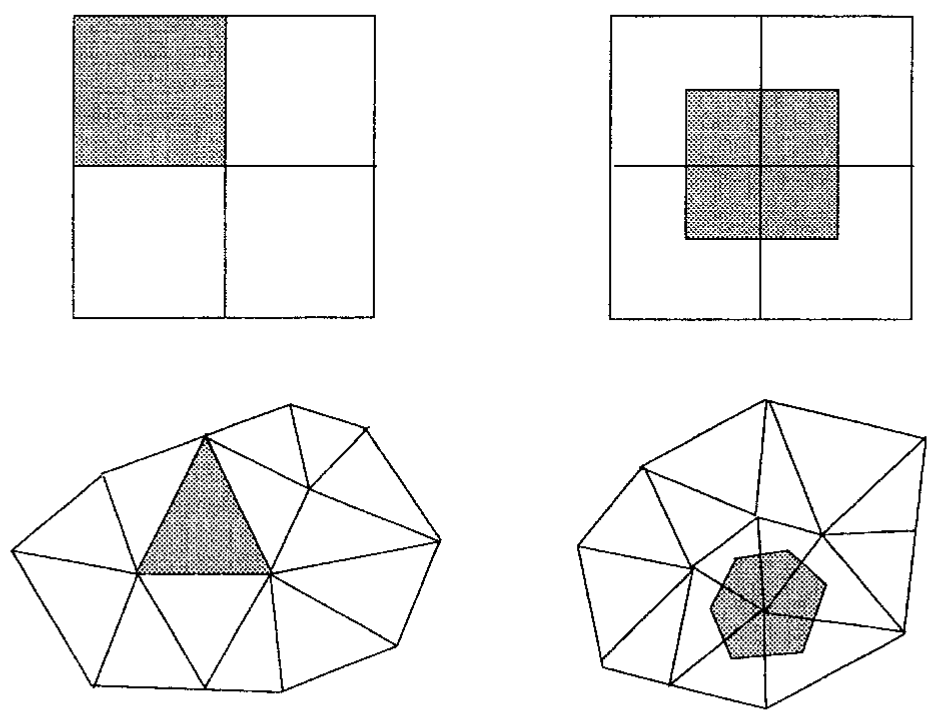
\includegraphics[width=.514\paperwidth]{images/fig-14-6-1.png}
  \caption{控制体积的例子}\label{fig:14.6.1}
\end{figure}

在\eqref{eq:14.6.8}中,下列选择会给出不同的离散形式：
\begin{enumerate}[label=\alph*.]
  \item 假定函数 \(\boldsymbol{w}\) 在 \(V_J\) 内所取的多项式形式.
  \item \(\boldsymbol{w}\) 的自由度.
  \item 边界通量的计算方式,即相邻控制体积之间的交换机制.
\end{enumerate}
通常,将\eqref{eq:14.6.8}中的体积分替换为
\begin{equation}\label{eq:14.6.9}
  \int_{V_J}\boldsymbol{\sigma}(\boldsymbol{w})\,\mathrm d\boldsymbol{x}
     \simeq(\boldsymbol{\sigma}(\boldsymbol{w}))_J\operatorname{meas}(V_J).
\end{equation}

\SourcePage{512}
这里,\((\boldsymbol{\sigma}(\boldsymbol{w}))_J\) 代表流动变量 \(\boldsymbol{\sigma}(\boldsymbol{w})\) 在控制体积 \(V_J\) 上的\emph{平均值}.若有源项,也采用同样的近似.

关于自由度的选择,可以采用\emph{单元中心}、\emph{单元顶点}或\emph{节点中心}逼近.矩形体积的情形见\figref{fig:14.6.2}.在单元中心有限体积法中,变量与单元关联,因而表示单元平均值,可以看成单元内某一点处的代表值.例如,对空间二阶的有限体积格式,可取单元的重心作为该点.单元顶点法和节点中心法都将变量与网格点关联.

在处理可压缩流动的 Euler 或 Navier--Stokes 方程等守恒律方程组时,可以用交错网格作有限体积离散.在这种情形下,不同物理未知量与不同的自由度关联.参见\BookCite{patankar1980}{Patankar(1980)}.

\begin{figure}[htbp]
  \centering
  \begin{subfigure}[t]{.202\paperwidth}
    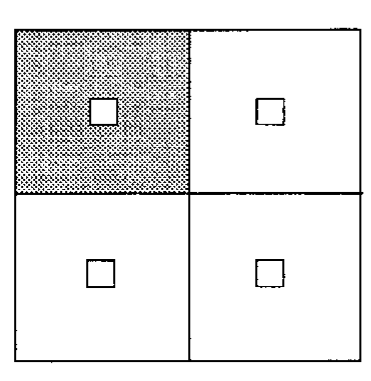
\includegraphics[width=\linewidth]{images/fig-14-6-2a.png}
    \caption{}\label{fig:14.6.2a}
  \end{subfigure}\hspace{.044\paperwidth}%
  \begin{subfigure}[t]{.216\paperwidth}
    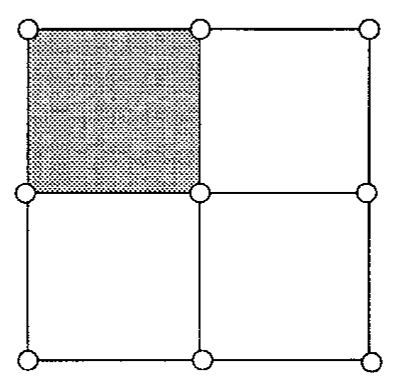
\includegraphics[width=\linewidth]{images/fig-14-6-2b.png}
    \caption{}\label{fig:14.6.2b}
  \end{subfigure}\hspace{.031\paperwidth}%
  \begin{subfigure}[t]{.216\paperwidth}
    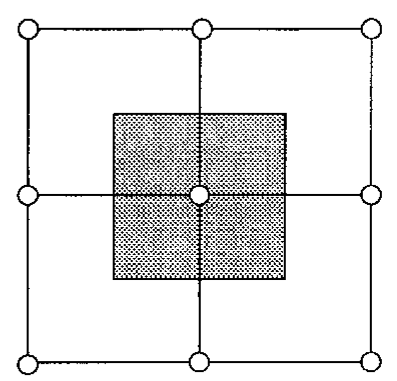
\includegraphics[width=\linewidth]{images/fig-14-6-2c.png}
    \caption{}\label{fig:14.6.2c}
  \end{subfigure}
  \caption{单元中心(a)、单元顶点(b)和节点中心(c)体积.阴影区域表示控制体积}\label{fig:14.6.2}
\end{figure}

就网格而言,有两类剖分：
\begin{enumerate}
  \item 类似有限差分网格,所有网格点都在两族线的交点上,例如两族分别平行于坐标轴的直线.这通常称为\emph{结构网格}.例子见\figref{fig:14.6.2}\subref{fig:14.6.2a}和\figref{fig:14.6.3}\subref{fig:14.6.3a}.
  \item 类似有限元网格,由三角形或四边形单元任意组合而成.网格点无法用一对整数来标识,需要逐点编号,并明确给出各顶点之间的连接关系.这类网格称为\emph{非结构网格}.例子见\figref{fig:14.6.2}\subref{fig:14.6.2b}和\figref{fig:14.6.3}\subref{fig:14.6.3b}.
\end{enumerate}
对于复杂几何构型,非结构网格更灵活.

采用结构网格,则很容易把计算区域映射为矩形区域.此外,将导数按各坐标线分开处理,便可将一维算法
\SourcePage{513}
推广到二维.结构网格也可以处理复杂几何,做法是把区域划分为多个块.

\begin{figure}[htbp]
  \centering
  \begin{subfigure}[t]{.315\paperwidth}
    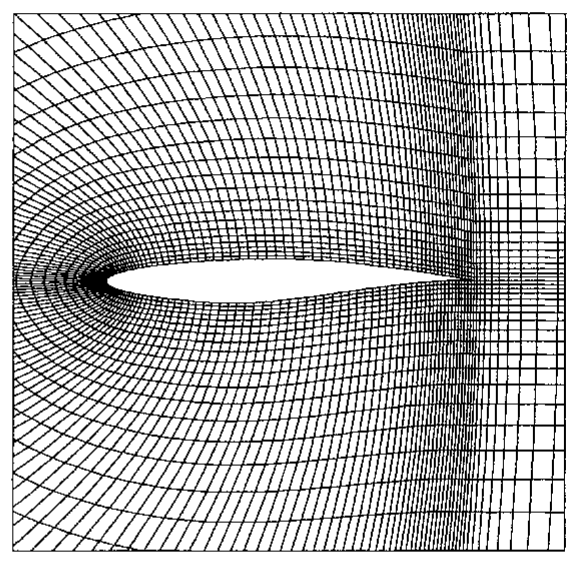
\includegraphics[width=\linewidth]{images/fig-14-6-3a.png}
    \caption{}\label{fig:14.6.3a}
  \end{subfigure}\hspace{.060\paperwidth}%
  \begin{subfigure}[t]{.312\paperwidth}
    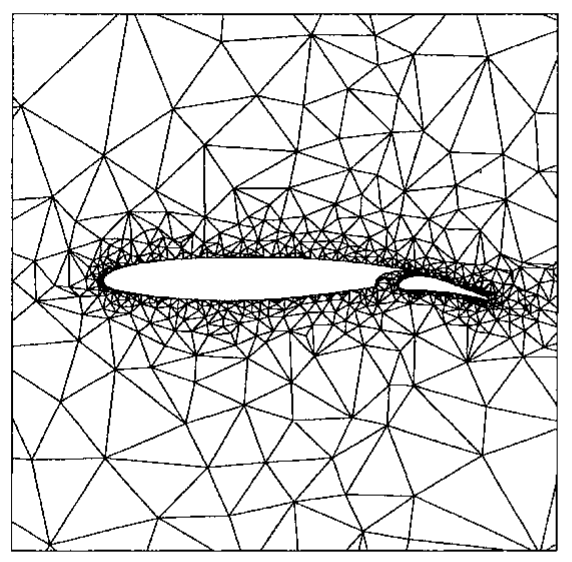
\includegraphics[width=\linewidth]{images/fig-14-6-3b.png}
    \caption{}\label{fig:14.6.3b}
  \end{subfigure}
  \caption{翼型周围的结构网格(a)和非结构网格(b)}\label{fig:14.6.3}
\end{figure}

在变量选取方面,单元中心离散常与结构网格配合使用.此时的难点是如何施加边界条件,因为代表单元值的网格点都不在区域边界 \(\partial\Omega\) 上.这一问题通常用外推法解决.节点中心法通常用于非结构网格.

有限体积法还有一个区别不同格式的关键方面,就是计算边界通量的策略.沿 \(\partial V_J\) 各边计算通量分量(见\eqref{eq:14.6.8})时,既要考虑所选格式,也要考虑流动变量的位置,即所选的自由度.基本上可以分为中心离散格式和迎风离散格式.

中心格式用对称的方式估计通量,计入界面两侧的贡献.这时需要在格式中人工加入适量的数值耗散,以防发生振荡.参见\BookCite{jameson-schmidt-turkel1981}{Jameson、Schmidt 和 Turkel(1981)}.

迎风格式根据各波分量的传播方向确定各边上的通量.下面简要讨论几个可用的准则.暂且不考虑黏性通量.第一种做法是在边 \(\Sigma\) 上,把法向通量 \(\boldsymbol{H}_{\rm inv}(\boldsymbol{w})\cdot\boldsymbol{n}=:\boldsymbol{H}_\Sigma(\boldsymbol{w})\) 换成依赖于两个状态(左、右或上、下)的数值通量函数 \(\boldsymbol{H}^{\rm num}(\boldsymbol{w}^l,\boldsymbol{w}^r)\).数值通量必须与精确通量一致,可以仿照第~\ref{sec:14.2.3}~节对一维标量双曲型方程的做法来选取.一种选法是先对前一时间层的两个状态 \(\boldsymbol{w}^l,\boldsymbol{w}^r\)
\SourcePage{514}
应用 Riemann 求解器,再计算 \(\boldsymbol{H}_\Sigma(\boldsymbol{w})\).例如,在结构网格上,可用第~\ref{sec:14.2.3}~节的有限差分逼近方式来实现.

也可采用更直接的做法.为简便起见,考虑\figref{fig:14.6.4}中的结构网格,它与单元中心有限体积法相对应.

设 \(V_J\) 为矩形 \(ABCD\),且 \(\boldsymbol{H}_{\rm inv}=(\boldsymbol{F}\mid\boldsymbol{G})\),其中 \(\boldsymbol{F},\boldsymbol{G}\) 是四维列向量,则
\begin{equation}\label{eq:14.6.10}
  \begin{aligned}
    \int_{\partial V_J}\boldsymbol{H}_{\rm inv}(\boldsymbol{w})\cdot\boldsymbol{n}\,\mathrm d\gamma
      &=\int_{AB}\boldsymbol{F}(\boldsymbol{w})\,\mathrm d\gamma
          +\int_{BC}\boldsymbol{G}(\boldsymbol{w})\,\mathrm d\gamma\\
      &\qquad-\int_{CD}\boldsymbol{F}(\boldsymbol{w})\,\mathrm d\gamma
          -\int_{DA}\boldsymbol{G}(\boldsymbol{w})\,\mathrm d\gamma,
  \end{aligned}
\end{equation}
其中各边上的 \(\mathrm d\gamma\) 均为正的弧长测度.在离散中,可用以下\emph{中心}格式逼近右端：
\begin{equation}\label{eq:14.6.11}
  \begin{aligned}
    &\boldsymbol{F}_{AB}|x_{B,2}-x_{A,2}|+\boldsymbol{G}_{BC}|x_{B,1}-x_{C,1}|\\
    &\qquad-\boldsymbol{F}_{CD}|x_{C,2}-x_{D,2}|
             -\boldsymbol{G}_{DA}|x_{A,1}-x_{D,1}|.
  \end{aligned}
\end{equation}
以 \(\boldsymbol{F}_{AB}\) 为例,可考虑几种选法.
\begin{enumerate}[label=\alph*.]
  \item 左右通量的平均：
    \begin{equation}\label{eq:14.6.12}
      \boldsymbol{F}_{AB}=\tfrac12(\boldsymbol{F}_{i+1,j}+\boldsymbol{F}_{i,j}),
      \qquad\boldsymbol{F}_{i,j}:=\boldsymbol{F}(\boldsymbol{w}_{i,j}),
    \end{equation}
    其中 \(\boldsymbol{w}_{i,j}\) 是 \(\boldsymbol{w}\) 在节点 \((i,j)\) 的值.
  \item 顶点通量的平均：
    \begin{equation}\label{eq:14.6.13}
      \boldsymbol{F}_{AB}=\tfrac12(\boldsymbol{F}_A+\boldsymbol{F}_B),
      \qquad\boldsymbol{F}_A:=\boldsymbol{F}(\boldsymbol{w}_A),\quad
            \boldsymbol{F}_B:=\boldsymbol{F}(\boldsymbol{w}_B),
    \end{equation}
    其中 \(\boldsymbol{w}_A\) 和 \(\boldsymbol{w}_B\) 分别是汇于点 \(A\) 和点 \(B\) 的四个单元上的 \(\boldsymbol{w}\) 值之和除以 \(4\).
  \item 变量平均后的通量：
    \begin{equation}\label{eq:14.6.14}
      \boldsymbol{F}_{AB}=\boldsymbol{F}\bigl(\tfrac12(\boldsymbol{w}_{i+1,j}+\boldsymbol{w}_{i,j})\bigr).
    \end{equation}
\end{enumerate}
其余通量也可类似计算.

对于单元顶点有限体积法,选法\eqref{eq:14.6.13}也很直接,不过此时 \(\boldsymbol{w}_A\) 和 \(\boldsymbol{w}_B\) 分别表示 \(\boldsymbol{w}\) 在顶点 \(A\) 和 \(B\) 的值.

不难看出,在均匀网格上,上述有限体积法实际上与有限差分格式一致.例如,若每个单元的大小为 \(\Delta x_1\times\Delta x_2\),选法\eqref{eq:14.6.12}导出二阶中心格式
\[
  \frac{\partial\boldsymbol{\sigma}(\boldsymbol{w}_{i,j})}{\partial t}
    +\frac{\boldsymbol{F}_{i+1,j}-\boldsymbol{F}_{i-1,j}}{2\Delta x_1}
    +\frac{\boldsymbol{G}_{i,j+1}-\boldsymbol{G}_{i,j-1}}{2\Delta x_2}=0.
\]

\SourcePage{515}
\begin{figure}[htbp]
  \centering
  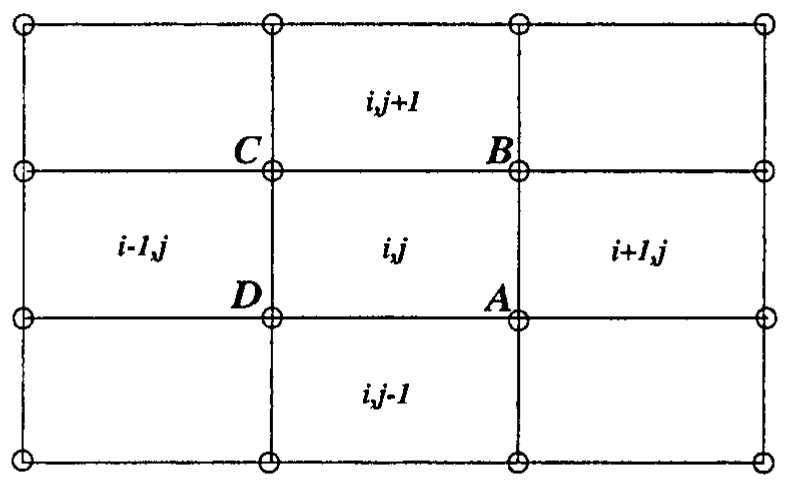
\includegraphics[width=.429\paperwidth]{images/fig-14-6-4.png}
  \caption{单元中心有限体积}\label{fig:14.6.4}
\end{figure}

如第~\ref{sec:14.2}~节所见,因此可以预期会发生振荡,这也提示我们在这里采用\emph{迎风}格式.也就是说,对流通量的计算取决于相应对流速度所决定的传播方向.对流速度由通量对守恒变量的 Jacob 矩阵给出.以 \(\boldsymbol{w}\) 表示守恒变量时,记为
\[
  A(\boldsymbol{w})=\frac{\partial\boldsymbol{H}_{\rm inv}(\boldsymbol{w})}{\partial\boldsymbol{w}}.
\]
对于给定的边,使用其法向通量的 Jacob 矩阵.

对于单元中心有限体积法,最简单的迎风格式令单元边通量等于上游单元所产生的通量.在均匀网格上,这给出标准的迎风有限差分格式.

对于单元顶点有限体积法,根据对流速度的符号,用 \(\boldsymbol{F}_{CD}\) 或 \(\boldsymbol{F}_{EF}\) 代替通量 \(\boldsymbol{F}_{AB}\).这里 \(EF\) 指 \(AB\) 右侧与它平行的下一条网格边.因此,所得格式的差分模板可能相当宽.

黏性通量,即\eqref{eq:14.6.8}中的 \(\int_{\partial V_J}\boldsymbol{H}_{\rm vis}(\boldsymbol{w})\cdot\boldsymbol{n}\,\mathrm d\gamma\),通常用中心格式计算.有时也采用有限元做法处理这些项,例如见\BookCite{rostand-stoufflet1988}{Rostand 和 Stoufflet(1988)}、\BookCite{tidriri1992}{Tidriri(1992)}及\BookCite{arminjon-dervieux1993}{Arminjon 和 Dervieux(1993)}.关于结构网格上可压缩 Navier--Stokes 方程的其他有限体积格式,见\BookCite{crumpton-mackenzie-morton1993}{Crumpton、Mackenzie 和 Morton(1993)}及其中的参考文献.

时间推进格式可以是显式的,也可以是隐式的.求定常解时,显式格式若配以适当的加速技术,也能有竞争力.这些技术包括局部时间步进、用于计算残差的多重网格技术,以及适当的残差光滑化.有关介绍,见\BookCite{johnson1983}{Johnson(1983)}、\BookCite{jameson1985}{Jameson(1985)}、\BookCite{koren1988}{Koren(1988)}、\BookCite{lallemand-koren1989}{Lallemand 和 Koren(1989)}、\BookCite{lallemand-steve-dervieux1992}{Lallemand、Steve 和 Dervieux(1992)}以及\BookCite{hemker-desideri1993}{Hemker 和 Desideri(1993)}.

对于非定常问题,隐式方法一般更高效,尤其是在高 Reynolds 数的黏性流动中.这些格式通常用所谓的增量形式实现,即每一步求解未知增量 \(\Delta\boldsymbol{w}^{(n)}:=\boldsymbol{w}^{n+1}-\boldsymbol{w}^n\).下面简述得到这一形式的办法.从\eqref{eq:14.6.1}出发,
\SourcePage{516}
用向后 Euler 格式推进时间,对每个控制体积 \(V_J\) 得到
\[
  \int_{V_J}\frac{\boldsymbol{\sigma}(\boldsymbol{w}^{n+1})-\boldsymbol{\sigma}(\boldsymbol{w}^n)}{\Delta t}
             \,\mathrm d\boldsymbol{x}
        +\int_{\partial V_J}\boldsymbol{\varphi}(\boldsymbol{w}^{n+1})\,\mathrm d\gamma=0.
\]
对含未知量的项作一阶 Taylor 展开,得到近似方程
\[
  \begin{aligned}
    &\frac1{\Delta t}\int_{V_J}
         \frac{\partial\boldsymbol{\sigma}}{\partial\boldsymbol{w}}(\boldsymbol{w}^n)
            \Delta\boldsymbol{w}^{(n)}\,\mathrm d\boldsymbol{x}
       +\int_{\partial V_J}\frac{\partial\boldsymbol{\varphi}}{\partial\boldsymbol{w}}(\boldsymbol{w}^n)
            \Delta\boldsymbol{w}^{(n)}\,\mathrm d\gamma\\
    &\qquad=-\int_{\partial V_J}\boldsymbol{\varphi}(\boldsymbol{w}^n)\,\mathrm d\gamma.
  \end{aligned}
\]
这可作为实现上述任一种有限体积格式的出发点.

\section{补充说明}\label{sec:14.7}

\BookCite{van-leer1992}{van Leer(1992)}综述了多维迎风有限差分法.\BookCite{coquel-lefloch1993}{Coquel 和 Le Floch(1993)}给出了一般收敛理论.

在有限元方面,非线性双曲型方程近年来得到了广泛研究.关于理论分析,可参见 Johnson 及其合作者的工作,例如\BookCite{johnson-szepessy1987}{Johnson 和 Szepessy(1987)}、\BookCite{johnson-szepessy-hansbo1990}{Johnson、Szepessy 和 Hansbo(1990)}和 Szepessy(\BookCite{szepessy1989}{1989}、\BookCite{szepessy1991}{1991}).关于在可压缩无黏流动中的数值应用,参见\BookCite{hughes-tezduyar1984}{Hughes 和 Tezduyar(1984)}、\BookCite{shakib1988}{Shakib(1988)}、\BookCite{lebeau-tezduyar1991}{Le Beau 和 Tezduyar(1991)}以及\BookCite{lebeau-ray-aliabadi-tezduyar1993}{Le Beau、Ray、Aliabadi 和 Tezduyar(1993)}.

有一种方法把有限元剖分的几何灵活性与类似有限差分的界面通量处理结合起来,后者采用类似 ENO 的做法.这便是\emph{间断 Galerkin--Runge--Kutta 法}的基础.相关的提出和分析见 Cockburn 和 Shu(\BookCite{cockburn-shu1989}{1989}、\BookCite{cockburn-shu1991}{1991})、\BookCite{cockburn-lin-shu1989}{Cockburn、Lin 和 Shu(1989)}以及\BookCite{cockburn-hou-shu1990}{Cockburn、Hou 和 Shu(1990)}.这种方法所得格式具有 TVB 性质.当用次数不超过 \(k\)(\(k\ge1\))的多项式定义有限元子空间时,格式具有 \(k\) 阶精度.

关于非线性双曲型方程的 Taylor--Galerkin 法综述,见\BookCite{donea-quartapelle1992}{Donea 和 Quartapelle(1992)}.

\backmatter
\cleardoublepage
\bookmarksetup{startatroot}
\chapter*{参考文献}
\addcontentsline{toc}{chapter}{参考文献}
\markboth{参考文献}{参考文献}
\begingroup
\small
\setlength{\parindent}{0pt}
\setlength{\parskip}{0.35em}
\setlength{\emergencystretch}{3em}
\newcommand{\RefEntry}[2]{\par\phantomsection#1\hangindent=1.5em\hangafter=1\relax #2\par}

\SourcePage{517}
\RefEntry{\label{bib:abarbanel-gottlieb-tadmor1986}}{S. Abarbanel, D. Gottlieb and E. Tadmor (1986), Spectral methods for discontinuous problems, in \textit{Numerical Methods for Fluid Dynamics II, }K.W. Morton and M.J. Baines eds., Oxford University Press, Oxford, pp. 129--153.}
\RefEntry{\label{bib:abramowitz-stegun1966}}{M. Abramowitz and I.A. Stegun, eds. (1966), \textit{Handbook of Mathematical Functions with Formulas, Graphs, and Mathematical Tables, }Dover, New York.}
\RefEntry{\label{bib:adams1975}}{R.A. Adams (1975), \textit{Sobolev Spaces, }Academic Press, New York.}
\RefEntry{\label{bib:agmon1965}}{S. Agmon (1965), \textit{Lectures on Elliptic Boundary Value Problems, }Van Nostrand, Princeton.}
\RefEntry{\label{bib:agoshkov1988}}{V.I. Agoshkov (1988), Poincare-Steklov's operators and domain decomposition methods in finite dimensional spaces, in \textit{First International Symposium on Domain Decomposition Methods for Partial Differential Equations, }R. Glowinski, G.H. Golub, G.A. Meurant and J. Périaux eds., SIAM, Philadelphia, pp. 73--112.}
\RefEntry{\label{bib:agoshkov-lebedev1985}}{V.I. Agoshkov and V.I. Lebedev (1985), Poincare-Steklov operators and the methods of partition of the domain in variational problems, in \textit{Computational Processes and Systems, No.2, }G.I. Marchuk ed., Nauka, Moscow, pp. 173--227 [Russian].}
\RefEntry{\label{bib:ainsworth-oden1993}}{M. Ainsworth and J.T. Oden (1993), A unified approach to a posteriori error estimation using element residual methods, Numer. Math. 65, 23--50.}
\RefEntry{\label{bib:ainsworth-zhu-craig-zienkiewicz1989}}{M. Ainsworth, J.Z. Zhu, A.W. Craig and O.C. Zienkiewicz (1989), Analysis of the Zienkiewicz-Zhu a posteriori error estimator in the finite element method, Internat. J. Numer. Methods Engrg. 28, 2161--2174.}
\RefEntry{\label{bib:allgower-georg1990}}{E.L. Allgower and K. Georg (1990), \textit{Numerical Continuation Methods: an Introduction, }Springer-Verlag, Berlin.}
\RefEntry{\label{bib:allgower-georg1993}}{E.L. Allgower and K. Georg (1993), Continuation and path following, Acta Numer., 1--64.}
\RefEntry{\label{bib:anderson-greengard1991}}{C.R. Anderson and C. Greengard, eds. (1991), \textit{Vortex Dynamics and Vortex Methods, }American Mathematical Society, Providence.}
\RefEntry{\label{bib:arminjon-dervieux1993}}{P. Arminjon and A. Dervieux (1993), Construction of TVD-like artificial viscosities on two-dimensional arbitrary FEM grids, J. Comput. Phys. 106, 176--198.}
\RefEntry{\label{bib:arnold-brezzi1985}}{D.N. Arnold and F. Brezzi (1985), Mixed and non-conforming finite element methods: implementation, post-processing and error estimates, M\textsuperscript{2}AN 19, 7--35.}
\RefEntry{\label{bib:arnold-brezzi-fortin1984}}{D.N. Arnold, F. Brezzi and M. Fortin (1984), A stable finite element for the Stokes equations, Calcolo 21, 337--344.}
\RefEntry{\label{bib:arnoldi1951}}{W.E. Arnoldi (1951), The principle of minimized iterations in the solution of matrix eigenvalue problem, Quart. Appl. Math. 9, 17--29.}
\RefEntry{\label{bib:atkinson1978}}{K.E. Atkinson (1978), \textit{An Introduction to Numerical Analysis, }John Wiley \& Sons, New York.}
\RefEntry{\label{bib:axelsson-barker1984}}{O. Axelsson and V.A. Barker (1984), \textit{Finite Element Solution of Boundary Value Problems. Theory and Computation, }Academic Press, Orlando.}
\RefEntry{\label{bib:babuska1971}}{I. Babuška (1971), Error bounds for the finite element method, Numer. Math. 16, 322--333.}

\SourcePage{518}
\RefEntry{\label{bib:babuska1973a}}{I. Babuška (1973a), The finite element method with Lagrangian multipliers, Numer. Math. 20, 179--192.}
\RefEntry{\label{bib:babuska1973b}}{I. Babuška (1973b), The finite element method with penalty, Math. Comput. 27, 221--228.}
\RefEntry{\label{bib:babuska1976}}{I. Babuška (1976), The selfadaptive approach in the finite element method, in \textit{The Mathematics of Finite Elements and Applications II, }J.R. Whiteman ed., Academic Press, New York, pp. 125--142.}
\RefEntry{\label{bib:babuska-aziz1972}}{I. Babuška and A.K. Aziz (1972), Survey lectures on the mathematical foundations of the finite element method, in \textit{The Mathematical Foundations of the Finite Element Method with Applications }to \textit{Partial Differential Equations, }A.K. Aziz ed., Academic Press, New York, pp. 3--359.}
\RefEntry{\label{bib:babuska-chandra-flaherty1983}}{I. Babuška, J. Chandra and J.E. Flaherty, eds. (1983), \textit{Adaptive Computational Methods for Partial Differential Equations, }SIAM, Philadelphia.}
\RefEntry{\label{bib:babuska-dorr1981}}{I. Babuška and M.R. Dorr (1981), Error estimates for the combined \textit{h }and p-version of the finite element method, Numer. Math. 37, 257--277.}
\RefEntry{\label{bib:babuska-miller1987}}{I. Babuška and A. Miller (1987), A feedback finite element method with a-posteriori error estimates. Part I: the finite element method and some basic properties of the a-posteriori estimator, Comput. Meth. Appl. Mech. Engrg. 61, 1--40.}
\RefEntry{\label{bib:babuska-oden-lee1977}}{I. Babuška, J.T. Oden and J.K. Lee (1977), Mixed-hybrid finite element approximations of second order elliptic boundary-value problems, Comput. Meth. Appl. Mech. Engrg. 11, 175--206.}
\RefEntry{\label{bib:babuska-osborn1980}}{I. Babuška and J. Osborn (1980), Analysis of finite element methods for second order boundary value problems using mesh dependent norms, Numer. Math. 34, 41--62.}
\RefEntry{\label{bib:babuska-rheinboldt1978a}}{I. Babuška and W.C. Rheinboldt (1978a), Error estimates for adaptive finite element computations, SIAM J. Numer. Anal. 12, 1597--1615.}
\RefEntry{\label{bib:babuska-rheinboldt1978b}}{I. Babuška and W.C. Rheinboldt (1978b), A posteriori error estimates for the finite element method, Internat. J. Numer. Methods Engrg. 15, 736--754.}
\RefEntry{\label{bib:babuska-suri1990}}{I. Babuška and M. Suri (1990), The p- and h-p versions of the finite element method, an overview, in \textit{Spectral and High Order Methods for Partial Differential Equations, }C. Canuto and A. Quarteroni eds., North-Holland, Amsterdam, pp. 5--26.}
\RefEntry{\label{bib:babuska-szabo-katz1981}}{I. Babuška, B.A. Szabó and I.N. Katz (1981), The p-version of the finite element method, SIAM J. Numer. Anal. 18, 512--545.}
\RefEntry{\label{bib:babuska-zienkiewicz-gago-arantes1986}}{I. Babuška, O.C. Zienkiewicz, J. Gago and E.R. de Arantes e Oliveira, eds. (1986), \textit{Accuracy Estimates and Adaptive Refinements in Finite Element Computations, }John Wiley \& Sons, Chichester.}
\RefEntry{\label{bib:baiocchi-brezzi1983}}{C. Baiocchi and F. Brezzi (1983), Optimal error estimates for linear parabolic problems under minimal regularity assumptions, Calcolo 20, 143--176.}
\RefEntry{\label{bib:baiocchi-brezzi1992}}{C. Baiocchi and F. Brezzi (1992), Stabilization of unstable numerical methods, in \textit{Problemi Attuali dell'Analisi e della Fisica Matematica, }P.E. Ricci ed., Taormina, pp. 59--64.}
\RefEntry{\label{bib:baiocchi-brezzi-franca1993}}{C. Baiocchi, F. Brezzi and L.P. Franca (1993), Virtual bubbles and Galerkin-least-squares type methods (Ga.L.S.), Comput. Meth. Appl. Mech. Engrg. 105, 125--141.}
\RefEntry{\label{bib:baker-bramble-thomee1977}}{G.A. Baker, J.H. Bramble and V. Thomée (1977), Single step Galerkin approximations for parabolic problems, Math. Comput. 31, 818--847.}
\RefEntry{\label{bib:baker-dougalis-karakashian1982}}{G.A. Baker, V.A. Dougalis and O.A. Karakashian (1982), On a higher order accurate fully discrete Galerkin approximation to the Navier-Stokes equations, Math. Comput. 39, 339--375.}
\RefEntry{\label{bib:bank-dupont1981}}{R.E. Bank and T. Dupont (1981), An optimal order process for solving elliptic finite element equations, Math. Comput. 36, 35--51.}

\SourcePage{519}
\RefEntry{\label{bib:bank-welfert1990}}{R.E. Bank and B.D. Welfert (1990), A comparison between the mini-element and the Petrov-Galerkin formulations for the generalized Stokes problem, Comput. Meth. Appl. Mech. Engrg. 83, 61--68.}
\RefEntry{\label{bib:bank-wieser1985}}{R.E. Bank and A. Wieser (1985), Some a posteriori error estimators for elliptic partial differential equations, Math. Comput. 44, 283--301.}
\RefEntry{\label{bib:barwell-george1976}}{V. Barwell and J.A. George (1976), A comparison of algorithms for solving symmetric indefinite systems of linear equations, ACM Trans. Math. Soft. 2, 242--251.}
\RefEntry{\label{bib:beale-majda1982}}{J.T. Beale and A. Majda (1982), Vortex methods. I: convergence in three dimensions, Math. Comput. 39, 1--27.}
\RefEntry{\label{bib:behr-franca-tezduyar1993}}{M.A. Behr, L.P. Franca and T.E. Tezduyar (1993), Stabilized finite element methods for the velocity-pressure-stress formulation of incompressible flows, Comput. Meth. Appl. Mech. Engrg. 104, 31--48.}
\RefEntry{\label{bib:bemelmans1981}}{J. Bemelmans (1981), Gleichgewichtsfiguren zaher Fliissigkeiten mit Oberflachenspannung, Analysis 1, 241--282.}
\RefEntry{\label{bib:begue-conca-murat-pironneau1988}}{C. Bègue, C. Conca, F. Murat and O. Pironneau (1988), Les équations de Stokes et de Navier-Stokes avec des conditions aux limites sur la pression, in \textit{Nonlinear Partial Differential Equations and Their Applications, Collège de France Seminar, Vol. IX, }H. Brezis and J.-L. Lions eds., Longman, Harlow, pp. 179--264.}
\RefEntry{\label{bib:benque-ibler-keramsi-labadie1980}}{J.P. Benqué, B. Ibler, A. Keramsi and G. Labadie (1980), A finite element method for Navier-Stokes equations, in \textit{Proceedings of the Third International Conference on Finite Elements in Flow Problems, vol. }1, D.H. Norrie ed., Banff, pp. 110--120.}
\RefEntry{\label{bib:bercovier1978}}{M. Bercovier (1978), Perturbation of a mixed variational problem, applications to mixed finite element methods, RA.1.R.O. Anal. Numer. 12, 211--236.}
\RefEntry{\label{bib:bercovier-pironneau1979}}{M. Bercovier and O. Pironneau (1979), Error estimates for finite element solution of the Stokes problem in the primitive variables, Numer. Math. 33, 211--224.}
\RefEntry{\label{bib:bergh-lofstrom1976}}{J. Bergh and J. Löfström (1976), \textit{Interpolation Spaces: an Introduction, }Springer-Verlag, Berlin.}
\RefEntry{\label{bib:bernardi-canuto-maday1988}}{C. Bernardi, C. Canuto and Y. Maday (1988), Generalized inf-sup condition for Chebyshev approximation of the Stokes problem, SIAM J. Numer. Anal. 25, 1237--1271.}
\RefEntry{\label{bib:bernardi-maday1989}}{C. Bernardi and Y. Maday (1989), Properties of some weighted Sobolev spaces, and application to spectral approximations, SIAM J. Numer. Anal. 26, 769--829.}
\RefEntry{\label{bib:bernardi-maday1992}}{C. Bernardi and Y. Maday (1992), \textit{Approximations Spectrales de Problemes aux Limites Elliptiques, }Springer-Verlag, Paris.}
\RefEntry{\label{bib:bernardi-maday-metivet1987}}{C. Bernardi, Y. Maday and B. Metivet (1987), Calcul de la pression dans la resolution spectrale du problema de Stokes, Rech. Aérospat., 1--21.}
\RefEntry{\label{bib:bernardi-raugel1985}}{C. Bernardi and G. Raugel (1985), A conforming finite element method for the time-dependent Navier-Stokes equations, SIAM J. Numer. Anal. 22, 455--473.}
\RefEntry{\label{bib:bjorck-plemmons-schneider1981}}{A. Björck, R.J. Plemmons and H. Schneider (1981), \textit{Large Scale Matrix Problems, }North-Holland, New York.}
\RefEntry{\label{bib:bjorstad1989}}{P.E. Bjørstad (1989), Multiplicative and additive Schwarz methods: convergence in the two-domain case, in \textit{Domain Decomposition Methods, }T.F. Chan, R. Glowinski, J. Périaux and O.B. Widlund eds., SIAM, Philadelphia, pp. 147--159.}
\RefEntry{\label{bib:bjorstad-widlund1986}}{P.E. Bjørstad and O.B. Widlund (1986), Iterative methods for the solution of elliptic problems on regions partitioned into substructures, SIAM J. Numer. Anal. 23, 1097--1120.}
\RefEntry{\label{bib:boland-nicolaides1983}}{J. Boland and R.A. Nicolaides (1983), Stability of finite elements under divergence constraints, SIAM J. Numer. Anal. 20, 722--731.}
\RefEntry{\label{bib:boris-book1973}}{J.P. Boris and D.L. Book (1973), Flux corrected transport, I. SHASTA, a fluid transport algorithm that works, J. Comput. Phys. 11, 38--69.}
\RefEntry{\label{bib:bourgat-glowinski-letallec-vidrascu1989}}{J.F. Bourgat, R. Glowinski, P. Le Tallec and M. Vidrascu (1989), Variational formulation and algorithm for trace operator in domain decomposition calculations, in \textit{Domain Decomposition Methods, }T.F. Chan, R. Glowinski, J. Périaux and O.B. Widlund eds., SIAM, Philadelphia, pp. 3--16.}

\SourcePage{520}
\RefEntry{\label{bib:boyd1989}}{J.P. Boyd (1989), \textit{Chebyshev and Fourier Spectral Methods, }Springer-Verlag, Berlin.}
\RefEntry{\label{bib:bramble1986}}{J.H. Bramble (1986), The construction of preconditioners for elliptic problems by substructuring, in \textit{Numerical Analysis, }J.P. Hennart ed., Springer-Verlag, Berlin, pp. 158--166.}
\RefEntry{\label{bib:bramble1993}}{J.H. Bramble (1993), \textit{Multigrid Methods, }Longman, Harlow.}
\RefEntry{\label{bib:bramble-pasciak1988}}{J.H. Bramble and J.E. Pasciak (1988), A preconditioning technique for indefinite systems resulting from mixed approximations of elliptic problems, Math. Comput. 50, 1--17.}
\RefEntry{\label{bib:bramble-pasciak-schatz1986a}}{J.H. Bramble, J.E. Pasciak and A.H. Schatz (1986a), An iterative method for elliptic problems on regions partitioned into substructures, Math. Comput. 46, 361--369.}
\RefEntry{\label{bib:bramble-pasciak-schatz1986b}}{J.H. Bramble, J.E. Pasciak and A.H. Schatz (1986b), The construction of preconditioners for elliptic problems by substructuring. I, Math. Comput. 47, 103--134.}
\RefEntry{\label{bib:bramble-pasciak-schatz1987}}{J.H. Bramble, J.E. Pasciak and A.H. Schatz (1987), The construction of preconditioners for elliptic problems by substructuring. II, Math. Comput. 49, 1--16.}
\RefEntry{\label{bib:bramble-pasciak-schatz1988}}{J.H. Bramble, J.E. Pasciak and A.H. Schatz (1988), The construction of preconditioners for elliptic problems by substructuring, III, Math. Comput. 51, 415--430.}
\RefEntry{\label{bib:bramble-pasciak-schatz1989}}{J.H. Bramble, J.E. Pasciak and A.H. Schatz (1989), The construction of preconditioners for elliptic problems by substructuring, IV, Math. Comput. 53, 1--24.}
\RefEntry{\label{bib:bramble-pasciak-xu1990}}{J.H. Bramble, J.E. Pasciak and J. Xu (1990), Parallel multilevel preconditioners, in \textit{Third International Symposium on Domain Decomposition Methods for Partial Differential Equations, }T.F. Chan, R. Glowinski, J. Périaux and O.B. Widlund eds., SIAM, Philadelphia, pp. 341--357.}
\RefEntry{\label{bib:bramble-schatz-thomee-wahlbin1977}}{J.H. Bramble, A.H. Schatz, V. Thomée and L. Wahlbin (1977), Some convergence estimates for semi-discrete Galerkin type approximations for parabolic equations, SIAM J. Numer. Anal. 14, 218--241.}
\RefEntry{\label{bib:bramble-thomee1974}}{J.H. Bramble and V. Thomée (1974), Discrete time Galerkin methods for a parabolic boundary value problem, Ann. Mat. Pura Appl. 101, 115--152.}
\RefEntry{\label{bib:brandt1977}}{A. Brandt (1977), Multi-level adaptive solution to boundary-value problems, Math. Comput. 31, 333--390.}
\RefEntry{\label{bib:brebbia-telles-wrobel1984}}{C.A. Brebbia, J.C.F. Telles and L.C. Wrobel (1984), \textit{Boundary Element Techniques. Theory and Applications in Engineering, }Springer-Verlag, Berlin.}
\RefEntry{\label{bib:brenan-campbell-petzold1989}}{K.E. Brenan, S.L. Campbell and L.R. Petzold (1989), \textit{Numerical Solution of Initial-Value Problems in Differential-Algebraic Equations, }North-Holland, New York.}
\RefEntry{\label{bib:bressan-quarteroni1986}}{N. Bressan and A. Quarteroni (1986), Analysis of Chebyshev collocation methods for parabolic equations, SIAM J. Numer, Anal. 23, 1138--1154.}
\RefEntry{\label{bib:brezis1983}}{H. Brezis (1983), \textit{Analyse Fonctionnelle, }Masson, Paris.}
\RefEntry{\label{bib:brezzi1974}}{F. Brezzi (1974), On the existence, uniqueness and approximation of saddle-point problems arising from Lagrange multipliers, R.A.I.R.O. Anal. Numér. 8, 129--151.}
\RefEntry{\label{bib:brezzi-bristeau-franca-mallet-roge1992}}{F. Brezzi, M.-O. Bristeau, L.P. Franca, M. Mallet and G. Rogé (1992), A relationship between stabilized finite element methods and the Galerkin method with bubble functions, Comput. Meth. Appl. Mech. Engrg. 96, 117--129.}
\RefEntry{\label{bib:brezzi-canuto-russo1989}}{F. Brezzi, C. Canuto and A. Russo (1989), A self-adaptive formulation for the Euler/Navier-Stokes coupling, Comput. Meth. Appl. Mech. Engrg. 73, 317--330.}
\RefEntry{\label{bib:brezzi-douglas1988}}{F. Brezzi, J. Douglas, Jr. (1988), Stabilized mixed methods for the Stokes problem, Numer. Math. 53, 225--235.}
\RefEntry{\label{bib:brezzi-douglas-duran-fortin1987}}{F. Brezzi, J. Douglas, Jr., R. Duran and M. Fortin (1987), Mixed finite elements for second order elliptic problems in three variables, Numer. Math. 51, 237--250.}
\RefEntry{\label{bib:brezzi-douglas-marini1985}}{F. Brezzi, J. Douglas, Jr. and L.D. Marini (1985), Two families of mixed finite elements for second order elliptic problems, Numer. Math. 47, 217--235.}
\RefEntry{\label{bib:brezzi-falk1991}}{F. Brezzi and R.S. Falk (1991), Stability of higher-order Hood-Taylor methods, SIAM J. Numer. Anal. 28, 581--590.}

\SourcePage{521}
\RefEntry{\label{bib:brezzi-fortin1991}}{F. Brezzi and M. Fortin (1991), \textit{Mixed and Hybrid Finite Element Methods, }Springer-Verlag, New York.}
\RefEntry{\label{bib:brezzi-gilardi1987}}{F. Brezzi and G. Gilardi (1987), Functional analysis \& Functional spaces, in \textit{Finite Element Handbook, }Chap. 1 \& 2, H. Kardestuncer ed., McGraw-Hill, New York.}
\RefEntry{\label{bib:brezzi-pitkaranta1984}}{F. Brezzi and J. Pitkäranta (1984), On the stabilization of finite element approximations of the Stokes equations, in \textit{Efficient Solutions of Elliptic Systems, }W. Hackbusch ed., Friedl. Vieweg \& Sohn, Braunschweig, pp. 11--19.}
\RefEntry{\label{bib:brezzi-rappaz-raviart1980}}{F. Brezzi, J. Rappaz and P.-A. Raviart (1980), Finite-dimensional approximation of nonlinear problems. Part I: branches of nonsingular solutions, Numer. Math. 36, 1--25.}
\RefEntry{\label{bib:brezzi-rappaz-raviart1981a}}{F. Brezzi, J. Rappaz and P.-A. Raviart (1981a), Finite-dimensional approximation of nonlinear problems. Part II: limit points, Numer. Math. 37, 1--28.}
\RefEntry{\label{bib:brezzi-rappaz-raviart1981b}}{F. Brezzi, J. Rappaz and P.-A. Raviart (1981b), Finite-dimensional approximation of nonlinear problems. Part III: simple bifurcation points, Numer. Math. 38, 1--30.}
\RefEntry{\label{bib:bristeau-glowinski-periaux1987}}{M.a. Bristeau, R. Glowinski and J. Périaux (1987), Numerical methods for the Navier-Stokes equations. Application to the simulation of compressible and incompressible viscous flows, Comput. Phys, Rep. 6, 73--187.}
\RefEntry{\label{bib:brooks-hughes1982}}{A.N. Brooks and T.J.R. Hughes (1982), Streamline Upwind/Petrov-Galerkin formulations for convection dominated flows with particular emphasis on the incompressible Navier-Stokes equations, Comput. Meth. Appl. Mech. Engrg. 32, 199--259.}
\RefEntry{\label{bib:brown-saad1990}}{P.N. Brown and Y. Saad (1990), Hybrid Krylov methods for nonlinear systems of equations, SIAM J. Sci. Stat. Comput. 11, 450--481.}
\RefEntry{\label{bib:bunch-rose1976}}{J.R. Bunch and D.J. Rose, eds. (1976), \textit{Sparse Matrix Computations, }Academic Press, New York.}
\RefEntry{\label{bib:butcher1987}}{J.C. Butcher (1987), \textit{The Numerical Analysis of Ordinary Differential Equations: Runge-Kutta and General Linear Methods, }John Wiley \& Sons, Chichester.}
\RefEntry{\label{bib:buzbee-dorr-georg-golub1971}}{B.L. Buzbee, F.W. Dorr, J.A. George and G.H. Golub (1971), The direct solution of the discrete Poisson equation on irregular regions, SIAM J. Numer. Anal. 8, 722--736.}
\RefEntry{\label{bib:buzbee-golub-nielson1970}}{B.L. Buzbee, G.H. Golub and C.V. Nielson (1970), On direct methods for solving Poisson's equation, SIAM J. Numer. Anal. 7, 627--656.}
\RefEntry{\label{bib:cahouet-chabard1988}}{J. Cahouet and J.P. Chabard (1988), Some fast 3-D finite element solvers for the generalized Stokes problem, Internat. J. Numer. Methods Fluids 8, 869--895.}
\RefEntry{\label{bib:cai1990}}{X.-C. Cai (1990), An additive Schwarz algorithm for nonselfadjoint elliptic equations, in \textit{Third International Symposium on Domain Decomposition Methods for Partial Differential Equations, }T.F. Chan, R. Glowinski, J. Périaux and O.B. Widlund eds., SIAM, Philadelphia, pp. 232--244.}
\RefEntry{\label{bib:cai1991}}{X.-C. Cai (1991), Additive Schwarz algorithms for parabolic convection-diffusion equations, Numer. Math. 60, 41--61.}
\RefEntry{\label{bib:canuto1988}}{C. Canuto (1988), Spectral methods and a maximum principle, Math. Comput. 51, 615--629.}
\RefEntry{\label{bib:canuto1994}}{C. Canuto (1994), Stabilization of spectral methods by finite elements bubble functions, Comput. Meth. Appl. Mech. Engrg. 116, 13--26.}
\RefEntry{\label{bib:canuto-hussaini-quarteroni-zang1988}}{C. Canuto, M.Y. Hussaini, A. Quarteroni and T.A. Zang (1988), \textit{Spectral Methods in Fluid Dynamics, }Springer-Verlag, New York.}
\RefEntry{\label{bib:canuto-pietra1991}}{C. Canuto and P. Pietra (1991), Boundary and interface conditions within a finite element preconditioner for spectral methods, J. Comput. Phys. 91, 310--343.}
\RefEntry{\label{bib:canuto-quarteroni1982}}{C. Canuto and A. Quarteroni (1982), Approximation results for orthogonal polynomials in Sobolev spaces, Math. Comput. 38, 67--86.}

\SourcePage{522}
\RefEntry{\label{bib:canuto-quarteroni1984}}{C. Canuto and A. Quarteroni (1984), Variational methods in the theoretical analysis of spectral approximations, in \textit{Spectral Methods for Partial Differential Equations, }R.G. Voigt, D. Gottlieb and M.Y. Hussaini eds., SIAM, Philadelphia, pp. 55--78.}
\RefEntry{\label{bib:canuto-quarteroni1985}}{C. Canuto and A. Quarteroni (1985), Preconditioned minimal residual methods for Chebyshev spectral calculations, J. Comput. Phys 60, 315--337.}
\RefEntry{\label{bib:canuto-quarteroni1987}}{C. Canuto and A. Quarteroni (1987), On the boundary treatment in spectral methods for hyperbolic systems, J. Comput. Phys. 71, 100--110.}
\RefEntry{\label{bib:canuto-russo1993}}{C. Canuto and A. Russo (1993), On the elliptic-hyperbolic coupling, I: the advection-diffusion equation via the x-formulation, M\textsuperscript{3}AS 3, 145--170.}
\RefEntry{\label{bib:canuto-sacchilandriani1986}}{C. Canuto and G. Sacchi Landriani (1986), Analysis of the Kleiser-Schumann method, Numer. Math. 50, 217--243.}
\RefEntry{\label{bib:carlenzoli-gervasio1992}}{C. Carlenzoli and P. Gervasio (1992), Effective numerical algorithms for the solution of algebraic systems arising in spectral methods, Appl. Numer. Math. 10, 87--113.}
\RefEntry{\label{bib:cauchy1847}}{A.L. Cauchy (1847), Méthode générale pour résolution des systèmes d’équations simultanées, C.R.H.A.S. Paris 25, 536--538.}
\RefEntry{\label{bib:chan1987}}{T.F. Chan (1987), Analysis of preconditioners for domain decomposition, SIAM J. Numer. Anal. 24, 382--390.}
\RefEntry{\label{bib:chan-mathew1991}}{T.F. Chan and T.P. Mathew (1991), An application of the probing technique to the vertex space method in domain decomposition, in \textit{Fourth International Symposium on Domain Decomposition Methods for Partial Differential Equations, }R. Glowinski, Yu.A. Kuznetsov, G. Meurant, J. Périaux and O.B. Widlund eds., SIAM, Philadelphia, pp. 101--111.}
\RefEntry{\label{bib:chen-du-tadmor1992}}{G.-Q. Chen, Q. Du and E. Tadmor (1992), Spectral viscosity approximations to multidimensional scalar conservation laws, Math. Comput. 61, 629--643.}
\RefEntry{\label{bib:chen-zhou1992}}{G. Chen and J. Zhou (1992), \textit{Boundary Element Methods, }Academic Press, London.}
\RefEntry{\label{bib:chinosi-comodi1991}}{C. Chinosi and M.L Comodi (1991), A new numerical approach to the Stokes problem, Numer. Meth. Partial Differ. Eq. 7, 363--374.}
\RefEntry{\label{bib:chorin1967}}{A.J. Chorin (1967), The numerical solution of the Navier-Stokes equations for an incompressible fluid, Bull. Amer. Math. Soc. 73, 928--93l.}
\RefEntry{\label{bib:chorin1968}}{A.J. Chorin (1968), Numerical solution of the Navier-Stokes equations, Math. Comput. 22, 745--762.}
\RefEntry{\label{bib:chorin1973}}{A.J. Chorin (1973), Numerical study of slightly viscous flow, J. Fluid Mech. 57, 785--796.}
\RefEntry{\label{bib:chorin1980}}{A.J. Chorin (1980), Vortex models and boundary layer instability, SIAM J. Sci. Stat. Comput. 1, 1--2l.}
\RefEntry{\label{bib:ciarlet1968}}{Ph.G. Ciarlet (1968), An \(O(h^2)\) method for a non-smooth boundary value problem, Aequationes Math. 2, 39--49.}
\RefEntry{\label{bib:ciarlet1978}}{Ph.G. Ciarlet (1978), \textit{The Finite Element Method for Elliptic Problems, }North-Holland, Amsterdam.}
\RefEntry{\label{bib:ciarlet1991}}{Ph.G. Ciarlet (1991), Basic error estimates for elliptic problems, in \textit{Handbook of Numerical Analysis, II, }Ph.G. Ciarlet and J.-L. Lions eds., North-Holland, Amsterdam, pp. 16--351.}
\RefEntry{\label{bib:ciarlet-destuynder1979}}{Ph.G. Ciarlet and P. Destuynder (1979), A justification of the two-dimensional linear plate model, J. Mecanique 18, 315--344.}
\RefEntry{\label{bib:cividini-quarteroni-zampieri1993}}{A. Cividini, A. Quarteroni and E. Zampieri (1993), Numerical solution of linear elastic problems by spectral collocation methods, Comput. Meth. Appl. Mech. Engrg. 104, 49--76.}
\RefEntry{\label{bib:clement1975}}{Ph. Clement (1975), Approximation by finite element functions using local regularization, R.A.LR.O. Anal. Numer. 9, 77--84.}
\RefEntry{\label{bib:cockburn-shu1989}}{B. Cockburn and C.-W. Shu (1989), TVB Runge-Kutta local projection discontinuous Galerkin finite element method for conservation laws II: general framework, Math. Comput. 52, 411--435.}

\SourcePage{523}
\RefEntry{\label{bib:cockburn-shu1991}}{B. Cockburn and C.-W. Shu (1991), The Runge-Kutta local projection \(\mathbb P^1\) discontinuous Galerkin finite element method for conservation laws, M\textsuperscript{2}AN 25, 337--361.}
\RefEntry{\label{bib:cockburn-hou-shu1990}}{B. Cockburn, S. Hou and C.-W. Shu (1990), The Runge-Kutta local projection discontinuous Galerkin finite element method for conservation laws IV: the multi-dimensional case, Math. Comput.54, 545--581.}
\RefEntry{\label{bib:cockburn-lin-shu1989}}{B. Cockburn, S.-Y. Lin and C.-W. Shu (1989), TVB Runge-Kutta local projection discontinuous Galerkin finite element method for conservation laws III: one-dimensional systems, J. Comput. Phys. 84, 90--113.}
\RefEntry{\label{bib:conca1984}}{C. Conca (1984), Approximation de quelques problemas de type Stokes par une methode d'elements finis mixtes, Numer. Math. 45, 75--91.}
\RefEntry{\label{bib:concus-golub1976}}{P. Concus and G.H. Golub (1976), A generalized conjugate gradient method for non-symmetric systems of linear equations, in \textit{Computing Methods in Applied Sciences and Engineering, }R. Glowinski and J.-L. Lions eds., Springer-Verlag, New York, pp. 56--65.}
\RefEntry{\label{bib:concus-golub-oleary1976}}{P. Concus, G.H. Golub and D.P. O'Leary (1976), A generalized conjugate gradient method for the numerical solution of elliptic partial differential equations, in \textit{Sparse Matrix Computations, }J.R. Bunch and D.J. Rose eds., Academic Press, New York, pp. 309--332.}
\RefEntry{\label{bib:coquel-lefloch1993}}{F. Coquel and Ph. Le Floch (1993), Convergence of finite difference schemes for conservation laws in several space dimension: a general theory, SIAM J. Numer. Anal. 30, 675--700.}
\RefEntry{\label{bib:courant-friedrichs1948}}{R. Courant and \textit{K.O. }Friedrichs (1948), \textit{Supersonic Flow and Shock Waves, }Interscience, New York.}
\RefEntry{\label{bib:courant-friedrichs-lewy1928}}{R. Courant, K.O. Friedrichs and H. Lewy (1928), Über die partiellen Differenzengleichungen der mathematischen Physik, Math. Ann. 100, 32--74.}
\RefEntry{\label{bib:courant-hilbert1953}}{R. Courant and D. Hilbert (1953), \textit{Methods of Mathematical Physics, I, }Interscience, New York.}
\RefEntry{\label{bib:crandall-majda1980}}{M.G. Crandall and A. Majda (1980), Monotone difference approximations for scalar conservations laws, Math. Comput. 34, 1--21.}
\RefEntry{\label{bib:crouzeix-mignot1984}}{M. Crouzeix and A.L. Mignot (1984), \textit{Analyse Numerique des Equations Differentielles, }Masson, Paris.}
\RefEntry{\label{bib:crouzeix-rappaz1990}}{M. Crouzeix and J. Rappaz (1990), \textit{On Numerical Approximation in Bifurcation Theory, }Masson, Paris.}
\RefEntry{\label{bib:crouzeix-raviart1973}}{M. Crouzeix and P.-A. Raviart (1973), Conforming and nonconforming finite element methods for solving the stationary Stokes equations, I, R.A.I.R.O. Anal. Numér. 7, 33--75.}
\RefEntry{\label{bib:crumpton-mackenzie-morton1993}}{P.I. Crumpton, J.A. Mackenzie and K.W. Morton (1993), Cell vertex algorithms for the compressible Navier-Stokes equations, J. Comput. Phys. 109, 1--15.}
\RefEntry{\label{bib:davis-rabinowitz1984}}{P.J. Davis and P. Rabinowitz (1984), \textit{Methods of Numerical Integration, }2nd ed., Academic Press, Orlando.}
\RefEntry{\label{bib:davis1984}}{S.F. Davis (1984), TVD finite difference schemes and artificial viscosity, ICASE Report n. 84--20, Hampton.}
\RefEntry{\label{bib:dawson-du1991}}{C.N. Dawson and Q. Du (1991), A domain decomposition method for parabolic equations based on finite elements, in \textit{Fourth International Symposium on Domain Decomposition Methods for Partial Differential Equations, }R. Glowinski, Yu.A. Kuznetsov, G. Meurant, J. Périaux and O.B. Widlund eds., SIAM, Philadelphia, pp. 255--263.}
\RefEntry{\label{bib:dawson-dupont1992}}{C.N. Dawson and T.F. Dupont (1992), Explicit-implicit conservative Galerkin domain decomposition procedures for parabolic problems, Math. Comput. 58, 21--34.}
\RefEntry{\label{bib:demkowicz-oden-babuska1992}}{L. Demkowicz, J.T. Oden and I. Babuška, eds. (1992), \textit{Reliability in Computational Mechanics, }North-Holland, Amsterdam.}

\SourcePage{524}
\RefEntry{\label{bib:demmel-heath-vandervorst1993}}{J.W. Demmel, M.T. Heath and H.A. van der Vorst (1993), Parallel numerical linear algebra, Acta Numer., 111--197.}
\RefEntry{\label{bib:deroeck-letallec1991}}{Y.-H. De Roeck and P. Le Tallec (1991), Analysis and test of a local domain-decomposition preconditioner, in \textit{Fourth International Symposium on Domain Decomposition Methods for Partial Differential Equations, }R. Glowinski, Yu.A. Kuznetsov, G. Meurant, J. Périaux and O.B. Widlund eds., SIAM, Philadelphia, pp. 112--128.}
\RefEntry{\label{bib:deville-mund1985}}{M.O. Deville and E.H. Mund (1985), Chebyshev pseudospectral solution of secondorder elliptic equations with finite element preconditioning, J. Comput. Phys. 60, 517--533.}
\RefEntry{\label{bib:deville-mund1990}}{M.O. Deville and R.H. Mund (1990), Finite element preconditioning for pseudospectral solutions of elliptic problems, SIAM J. Sci. Stat. Comput. 11, 311--342.}
\RefEntry{\label{bib:devulder-marion-titi1993}}{C. Devulder, M. Marion and E.S. Titi (1993), On the rate of convergence of non-linear Galerkin methods, Math. Comput. 60, 495--514.}
\RefEntry{\label{bib:donea1984}}{J. Donea (1984), A Taylor-Galerkin method for convective transport problems, Internat. J. Numer. Methods Engrg. 20, 101--120.}
\RefEntry{\label{bib:donea-quartapelle1992}}{J. Donea and L. Quartapelle (1992), An introduction to finite element methods for transient advection problems, Comput. Meth. Appl. Mech. Engrg. 95, 169--203.}
\RefEntry{\label{bib:donea-quartapelle-selmin1987}}{J. Donea, L. Quartapelle and V. Selmin (1987), An analysis of time discretization in the finite element solution of hyperbolic problems, J. Comput. Phys. 70, 463--499.}
\RefEntry{\label{bib:dongarra-duff-sorensen-vandervorst1991}}{J.J. Dongarra, I.S. Duff, D.C. Sorensen and H.A. van der Vorst (1991), \textit{Solving Linear Systems on Vector and Shared Memory Computers, }SIAM, Philadelphia.}
\RefEntry{\label{bib:dorr1970}}{F.W. Dorr (1970), The direct solution of the discrete Poisson equation on a rectangle, SIAM Rev. 12, 248--263.}
\RefEntry{\label{bib:dorr1986}}{M.R. Dorr (1986), The approximation of solutions of elliptic boundary value problems via the p-version of the finite element method, SIAM J. Numer. Anal. 23, 58--77.}
\RefEntry{\label{bib:douglas-douglas1993}}{\textit{C.C. }Douglas and J. Douglas, Jr. (1993), A unified convergence theory for abstract multigrid or multilevel algorithms, serial and parallel, SIAM J. Numer. Anal. 30, 136--158.}
\RefEntry{\label{bib:douglas1955}}{J. Douglas, Jr. (1955), On the numerical integration of \textit{Ux x }+ \textit{U y y }= \textit{Ut }by implicit methods, J. SIAM 3, 42--65.}
\RefEntry{\label{bib:douglas-dupont1970}}{J. Douglas, Jr. and T. Dupont (1970), Galerkin methods for parabolic equations, SIAM J. Numer. Anal. 7, 575--626.}
\RefEntry{\label{bib:douglas-rachford1956}}{J. Douglas, Jr. and H.H. Rachford, Jr. (1956), On the numerical solution of heat conduction problems in two and three space variables, Trans. Amer. Math. Soc. 82, 421--439.}
\RefEntry{\label{bib:douglas-roberts1985}}{J. Douglas, Jr. and J.E. Roberts (1985), Global estimates for mixed methods for second order elliptic problems, Math. Comput. 44, 39--52.}
\RefEntry{\label{bib:douglas-russell1982}}{J. Douglas, Jr. and T.F. Russell (1982), Numerical mathods for convection-dominated diffusion problems based on combining the method of characteristics with finite element or finite difference procedures, SIAM J. Numer. Anal. 19, 871--885.}
\RefEntry{\label{bib:douglas-wang1989}}{J. Douglas, Jr. and J. Wang (1989), An absolutely stabilized finite element method for the Stokes problem, Math. Comput. 52, 495--508.}
\RefEntry{\label{bib:dryja1982}}{M. Dryja (1982), A capacitance matrix method for Dirichlet problem on polygon region, Numer. Math. 39, 51--64.}
\RefEntry{\label{bib:dryja1983}}{M. Dryja (1983), A finite element-capacitance matrix method for the elliptic problem, SIAM J. Numer. Anal. 20, 671--680.}
\RefEntry{\label{bib:dryja1984}}{M. Dryja (1984), A finite element-capacitance method for elliptic problems on regions partitioned into subregions, Numer. Math. 44, 153--168.}

\SourcePage{525}
\RefEntry{\label{bib:dryja1989}}{M. Dryja (1989), An additive Schwarz algorithm for two- and three-dimensional finite element elliptic problems, in \textit{Domain Decomposition Methods, }T.F. Chan, R. Glowinski, J. Périaux and O.B. Widlund eds., SIAM, Philadelphia, pp. 168--172.}
\RefEntry{\label{bib:dryja1991}}{M. Dryja (1991), Substructuring methods for parabolic problems, in \textit{Fourth International Symposium on Domain Decomposition Methods for Partial Differential Equations, }R. Glowinski, Yu.A. Kuznetsov, G. Meurant, J. Périaux and O.B. Widlund eds., SIAM, Philadelphia, pp. 264--271.}
\RefEntry{\label{bib:dryja-widlund1987}}{M. Dryja and O.B. Widlund (1987), An additive variant of the Schwarz alternating method for the case of many subregions, Technical Report 339, Department of Computer Science, Courant Institute of Mathematical Sciences, New York University.}
\RefEntry{\label{bib:dryja-widlund1990}}{M. Dryja and O.B. Widlund (1990), Towards a unified theory of domain decomposition algorithms for elliptic problems, in \textit{Third International Symposium on Domain Decomposition Methods for Partial Differential Equations, }T.F. Chan, R. Glowinski, J. Périaux and O.B. Widlund eds., SIAM, Philadelphia, pp. 3--21.}
\RefEntry{\label{bib:dryja-widlund1992}}{M. Dryja and O.B. Widlund (1992), Additive Schwarz methods for elliptic finite element problems in three dimensions, in \textit{Fifth International Symposium on Domain Decomposition Methods for Partial Differential Equations, }D.E. Keyes, T.F. Chan, G. Meurant, J.S. Scroggs and R.G. Voigt eds., SIAM, Philadelphia, pp. 3--18.}
\RefEntry{\label{bib:duff-erisman-reid1986}}{I.S. Duff, A.M. Erisman and J.K. Reid (1986), \textit{Direct Methods for Sparse Matrices, }Oxford University Press, Oxford.}
\RefEntry{\label{bib:dupont1982}}{T. Dupont (1982), Mesh modification for evolution equations, Math. Comput. 39, 85--107.}
\RefEntry{\label{bib:dupont-scott1980}}{T. Dupont and R. Scott (1980), Polynomial approximation of functions in Sobolev spaces, Math. Comput. 34, 441--463.}
\RefEntry{\label{bib:eisenstat-elman-schultz1983}}{S.C. Eisenstat, H.C. Elman and M.H. Schultz (1983), Variational iterative methods for non-symmetric systems of linear equations, SIAM J. Numer. Anal. 20, 354--361.}
\RefEntry{\label{bib:elman-saad-saylor1986}}{H.C. Elman, Y. Saad and P.E. Saylor (1986), A hybrid Chebyshev Krylov subspace algorithm for solving non-symmetric systems of linear equations, SIAM J. Sci. Stat. Comput. 7, 840--855.}
\RefEntry{\label{bib:erdos1961}}{P. Erdos (1961), Problems and results on the theory of interpolation, II, Acta Math. Acad. Sci. Hungar. 12, 235--244.}
\RefEntry{\label{bib:eriksson-estep-hansbo-johnson1995}}{K. Eriksson, D. Estep, P. Hansbo and C. Johnson (1995), Introduction to adaptive methods for differential equations, Acta Numer., 105--158.}
\RefEntry{\label{bib:eriksson-johnson-thomee1985}}{K. Eriksson, C. Johnson and V. Thomée (1985), Time discretization of parabolic problems by the discontinuous Galerkin method, M\textsuperscript{2}AN 19, 611--643.}
\RefEntry{\label{bib:ernst-golub1994}}{O. Ernst and G.H. Golub (1994), A domain decomposition approach to solving the Helmholtz equation via a radiation boundary condition, in \textit{Domain Decomposition Methods in Science and Engineering, }A. Quarteroni, J. Périaux, Yu.A. Kuznetsov and O.B. Widlund eds., American Mathematical Society, Providence, pp. 177--192.}
\RefEntry{\label{bib:evans1983}}{D.J. Evans, ed. (1983), \textit{Preconditioning Methods: Analysis and Applications, }Gordon \& Breach, New York.}
\RefEntry{\label{bib:ewing-russell-wheeler1984}}{R.E. Ewing, T.F. Russell and M.F. Wheeler (1984), Simulation of miscible displacements using mixed methods and a modified method of characteristics, Comput. Meth. Appl. Mech. Engrg. 47, 73--92.}
\RefEntry{\label{bib:falk-osborn1980}}{R.S. Falk and J.E. Osborn (1980), Error estimates for mixed methods, R.A.I.R.O. Anal. Numér. 14, 249--277.}

\SourcePage{526}
\RefEntry{\label{bib:falk-richter1992}}{R.S. Falk and G.R. Richter (1992), Local error estimates for a finite element method for hyperbolic and convection-diffusion equations, SIAM J. Numer. Anal. 29, 730--754.}
\RefEntry{\label{bib:fletcher1988a}}{C.A.J. Fletcher (1988a), \textit{Computational Techniques for Fluid Dynamics. }1. \textit{Fundamental and General Techniques, }Springer-Verlag, Berlin.}
\RefEntry{\label{bib:fletcher1988b}}{C.A.J. Fletcher (1988b), \textit{Computational Techniques for Fluid Dynamics. }2. \textit{Specific Techniques for Different Flow Categories, }Springer-Verlag, Berlin.}
\RefEntry{\label{bib:fletcher1976}}{R. Fletcher (1976), Conjugate gradient methods for indefinite systems, in \textit{Numerical Analysis, }G.A. Watson ed., Springer-Verlag, Berlin, pp. 73--89.}
\RefEntry{\label{bib:foias-jolly-kevrekidis-titi1991}}{C. Foias, M. Jolly, I. Kevrekidis and E.S. Titi (1991), Dissipativity of numerical schemes, Nonlinearity 4, 591--631.}
\RefEntry{\label{bib:foias-manley-temam1988}}{C. Foias, O. Manley and R. Temam (1988), Modelling of the interaction of small and large eddies in two dimensional turbulent flows, M\textsuperscript{2}AN 22, 93--114.}
\RefEntry{\label{bib:forsythe-wasow1960}}{G.E. Forsythe and W.R. Wasow (1960), \textit{Finite Difference Methods for Partial Differential Equations, }John Wiley \& Sons, New York.}
\RefEntry{\label{bib:fortin1972}}{M. Fortin (1972), \textit{Calcul Numerique des Ecoulements des Fluides de Bingham et des Fluides Newtonians Incompressibles par Ie Methode des Elements Finis, }These, Universite de Paris VI, Paris.}
\RefEntry{\label{bib:fortin1977}}{M. Fortin (1977), An analysis of the convergence of mixed finite element methods, R.A.1.R.O. Anal. Numer. 11, 341--354.}
\RefEntry{\label{bib:fortin1989}}{M. Fortin (1989), Some iterative methods for incompressible flow problems, Comput. Phys. Comm. 53, 393--399.}
\RefEntry{\label{bib:fortin1993}}{M. Fortin (1993), Finite element solution of the Navier-Stokes equations, Acta Numer., 239--284.}
\RefEntry{\label{bib:fortin-glowinski1983}}{M. Fortin and R. Glowinski (1983), \textit{Augmented Lagrangian Methods: Applications to the Numerical Solution of Boundary- Value Problems, }North-Holland, Amsterdam.}
\RefEntry{\label{bib:fortin-pierre1992}}{M. Fortin and R. Pierre (1992), Stability analysis of discrete generalized Stokes problems, Numer. Meth. Partial Differ. Eq. 8, 303--323.}
\RefEntry{\label{bib:fraeijsdeveubeke1965}}{B. Fraeijs de Veubeke (1965), Displacement and equilibrium models in the finite element method, in \textit{Stress Analysis, }O.C. Zienkiewicz and G.S. Holister eds., John Wiley \& Sons, New York, pp. 145--197.}
\RefEntry{\label{bib:franca-frey1992}}{L.P. Franca and S.L. Frey (1992), Stabilized finite element methods: I.I. The incompressible Navier-Stokes equations, Comput. Meth. Appl. Mech. Engrg. 99, 209--233.}
\RefEntry{\label{bib:franca-frey-hughes1992}}{L.P. Franca, S.L. Frey and T.J.R. Hughes (1992), Stabilized finite element methods, 1. Application to the advective-diffusive model, Comput. Meth. Appl. Mech. Engrg. 95, 253--276.}
\RefEntry{\label{bib:franca-stenberg1991}}{L.P. Franca and R. Stenberg (1991), Error analysis of some Galerkin least squares methods for the elasticity equations, SIAM J. Numer. Anal. 28, 1680--1697.}
\RefEntry{\label{bib:frati-pasquarelli-quarteroni1993}}{A. Frati, F. Pasquarelli and A. Quarteroni (1993), Spectral approximation to advection-diffusion problems by the fictitious interface method, J. Comput. Phys. 107, 201--212.}
\RefEntry{\label{bib:fujita-suzuki1991}}{H. Fujita and T. Suzuki (1991), Evolution problems, in \textit{Handbook of Numerical Analysis, II, }Ph.G. Ciarlet and J.-L. Lions eds., North-Holland, Amsterdam, pp. 789--928.}
\RefEntry{\label{bib:funaro1981}}{D. Funaro (1981), \textit{Approssimazione Numerica di Problem Parabolici }e \textit{Iperbolici con Metodi Spettrali, }Tesi, Universita di Pavia, Pavia.}
\RefEntry{\label{bib:funaro1986}}{D. Funaro (1986), A multidomain spectral approximation of elliptic equations, Numer. Meth. Partial Differ. Eq. 2, 187--205.}
\RefEntry{\label{bib:funaro1988}}{D. Funaro (1988), Domain decomposition methods for pseudospectral approximations. Part I: second order equations in one dimension, Numer. Math. 52, 325--344.}

\SourcePage{527}
\RefEntry{\label{bib:funaro1992}}{D. Funaro (1992), \textit{Polynomial Approximation of Differential Equations, }Springer-Verlag, Berlin.}
\RefEntry{\label{bib:funaro-gottlieb1988}}{D. Funaro and D. Gottlieb (1988), A new method of imposing boundary conditions in pseudospectral approximation of hyperbolic equations, Math. Comput. 51, 599--613.}
\RefEntry{\label{bib:funaro-gottlieb1989}}{D. Funaro and D. Gottlieb (1989), Convergence results for pseudospectral approximations of hyperbolic systems, ICASE Report n. 89--59, Hampton.}
\RefEntry{\label{bib:funaro-quarteroni-zanolli1988}}{D. Funaro, A. Quarteroni and P. Zanolli (1988), An iterative procedure with interface relaxation for domain decomposition methods, SIAM J. Numer. Anal. 25, 1213--1236.}
\RefEntry{\label{bib:galeao-dutradocarmo1988}}{A.C. Galeão and E.G. Dutra do Carmo (1988), A consistent approximate upwind Petrov-Galerkin method for convection-dominated problems, Comput. Meth. Appl. Mech. Engrg. 68, 83--95.}
\RefEntry{\label{bib:gastaldi-quarteroni1989}}{F. Gastaldi and A. Quarteroni (1989), On the coupling of hyperbolic and parabolic systems: analytical and numerical approach, Appl. Numer. Math. 6, 3--31.}
\RefEntry{\label{bib:gastaldi-quarteroni-sacchilandriani1990}}{F. Gastaldi, A. Quarteroni and G. Sacchi Landriani (1990), On the coupling of two dimensional hyperbolic and elliptic equations: analytical and numerical approach, in \textit{Third International Symposium on Domain Decomposition Methods for Partial Differential Equations, }T.F. Chan, R. Glowinski, J. Périaux and O.B. Widlund eds., SIAM, Philadelphia, pp. 22--63.}
\RefEntry{\label{bib:gastaldi-nochetto1987}}{L. Gastaldi and R. Nochetto (1987), Optimal \(L^\infty\)-estimates for nonconforming and mixed finite element methods of lowest order, Numer. Math. 50, 587--611.}
\RefEntry{\label{bib:gear1971}}{C.W. Gear (1971), \textit{Numerical Initial Value Problems in Ordinary Differential Equations, }Prentice-Hall, Englewood Cliffs.}
\RefEntry{\label{bib:george-liu1981}}{J.A. George and J.W.H. Liu (1981), \textit{Computer Solution of Large Sparse Positive Definite Systems, }Prentice-Hall, Englewood Cliffs.}
\RefEntry{\label{bib:girault1988}}{V. Girault (1988), Incompressible finite element methods for Navier-Stokes equations with nonstandard boundary conditions in R3 , Math. Comput. 51, 55--74.}
\RefEntry{\label{bib:girault1990}}{V. Girault (1990), Curl-conforming finite element methods for Navier-Stokes equations with non-standard boundary conditions in R3 , in \textit{The Navier-Stokes Equations. Theory and Numerical Methods, }J.G. Heywood, K. Masuda, R Rautmann and V.A. Solonnikov eds., Springer-Verlag, Berlin, pp. 201--218.}
\RefEntry{\label{bib:girault-raviart1986}}{V. Girault and P.-A. Raviart (1986), \textit{Finite Element Methods for Navier-Stokes Equations, }Springer-Verlag, Berlin.}
\RefEntry{\label{bib:glowinski1984}}{R. Glowinski (1984), \textit{Numerical Methods for Nonlinear Variational Problems, }Springer-Verlag, New York.}
\RefEntry{\label{bib:glowinski-dinh-periaux1983}}{R. Glowinski, Q.V. Dinh and J. Périaux (1983), Domain decomposition methods for nonlinear problems in fluid dynamics, Comput. Meth. Appl. Mech. Engrg. 40, 27--109.}
\RefEntry{\label{bib:glowinski-letallec1989}}{R. Glowinski and P. Le Tallec (1989), \textit{Augmented Lagrangian and Operator-Splitting Methods in Nonlinear Mechanics, }SIAM, Philadelphia.}
\RefEntry{\label{bib:glowinski-letallec1990}}{R. Glowinski and P. Le Tallec (1990), Augmented Lagrangian interpretation of the nonoverlapping Schwarz alternating method, in \textit{Third International Symposium on Domain Decomposition Methods for Partial Differential Equations, }T.F. Chan, R. Glowinski, J. Périaux and O.B. Widlund eds., SIAM, Philadelphia, pp. 224--231.}
\RefEntry{\label{bib:glowinski-mantel-periaux-perrier-pironneau1982}}{R. Glowinski, B. Mantel, J. Périaux, P. Perrier and O. Pironneau (1982), On an efficient new preconditioned conjugate gradient method. Application to the incore solution of the Navier-Stokes equations via nonlinear least-squares and finite element methods, in \textit{Finite Elements in Fluids, Vol. }4, R.H. Gallagher, D.H. Norrie, J.T. Oden and O.C. Zienkiewicz eds., John Wiley \& Sons, Chichester, pp. 365--401.}

\SourcePage{528}
\RefEntry{\label{bib:glowinski-pan-periaux1993}}{R. Glowinski, T.W. Pan and J. Périaux (1993), Fictitious domain method for the Dirichlet problem and its generalization to some flow problems, in \textit{Finite Elements in Fluids. New Trends and Applications, }K. Morgan, E. Oñate, J. Périaux and J. Peraire eds., Pineridge Press, Swansea, pp. 347--368.}
\RefEntry{\label{bib:glowinski-pan-periaux1994}}{R. Glowinski, T.W. Pan and J. Périaux (1994), A fictitious domain method for unsteady incompressible viscous flow modeled by Navier-Stokes equations, in \textit{Domain Decomposition Methods in Science and Engineering, }A. Quarteroni, J. Périaux, Yu.A. Kuznetsov and O.B. Widlund eds., American Mathematical Society, Providence, pp. 421--430.}
\RefEntry{\label{bib:glowinski-pironneau1979}}{R. Glowinski and O. Pironneau (1979), On mixed finite element approximation of the Stokes problem (I) Numer. Math. 33, 397--424.}
\RefEntry{\label{bib:godlewski-raviart1991}}{E. Godlewski and P.-A. Raviart (1991), \textit{Hyperbolic Systems of Conservations Laws, }Ellipse, Paris.}
\RefEntry{\label{bib:godunov-ryabenkii1987}}{S.K. Godunov and V.S. Ryabenkiĭ (1987), \textit{Theory of Difference Schemes. An Introduction to the Underlying Theory, }North-Holland, Amsterdam. Russian ed.: Gosudarstv. Izdat. Fiz.-Mat. Lit., Moscow, 1962.}
\RefEntry{\label{bib:golub-mayers1984}}{G.H. Golub and D. Mayers (1984), The use of pre-conditioning over irregular regions, in \textit{Computing Methods in Applied Sciences and Engineering, VI, }R. Glowinski and J.-L. Lions eds., North-Holland, Amsterdam, pp. 3--14.}
\RefEntry{\label{bib:golub-oleary1989}}{G.H. Golub and D.P. O'Leary (1989), Some history of the conjugate gradient and Lanczos algorithms: 1948--1976, SIAM Rev. 31, 50--102.}
\RefEntry{\label{bib:golub-ortega1993}}{G.H. Golub and J.M. Ortega (1993), \textit{Scientific Computing. An Introduction with Parallel Computing, }Academic Press, San Diego.}
\RefEntry{\label{bib:golub-vanloan1989}}{G.H. Golub and C.F. Van Loan (1989), \textit{Matrix Computations, }2nd ed., The Johns Hopkins University Press, Baltimore.}
\RefEntry{\label{bib:gottlieb1985}}{D. Gottlieb (1985), Spectral methods for compressible flow problems, in \textit{Ninth International Conference on Numerical Methods in Fluid Dynamics, }Soubbarameyer and J.-P. Boujot eds., Springer-Verlag, Berlin, pp. 48--61.}
\RefEntry{\label{bib:gottlieb-gunzburger-turkel1982}}{D. Gottlieb, M.D. Gunzburger and E. Turkel (1982), On numerical boundary treatment for hyperbolic systems, SIAM J. Numer. Anal. 19, 671--697.}
\RefEntry{\label{bib:gottlieb-lustman1983}}{D. Gottlieb and L. Lustman (1983), The spectrum of the Chebyshev collocation operator for the heat equation, SIAM J. Numer. Anal. 20, 908--921.}
\RefEntry{\label{bib:gottlieb-orszag1977}}{D. Gottlieb and S.A. Orszag (1977), \textit{Numerical Analysis of Spectral Methods: Theory and Applications, }SIAM, Philadelphia.}
\RefEntry{\label{bib:gottlieb-tadmor1985}}{D. Gottlieb and E. Tadmor (1985), Recovering pointwise values of discontinuous data within spectral accuracy, in \textit{Progress and Supercomputing in Computational Fluid Dynamics, }E.M. Murman and S.S. Abarbanel eds., Birkhäuser Verlag, Boston, pp. 357--375.}
\RefEntry{\label{bib:gresho1990}}{P.M. Gresho (1990), On the theory of semi-implicit projection methods for viscous incompressible flow and its implementation via a finite element method that also introduces a nearly consistent mass matrix. Part 1: Theory, Internat. J. Numer. Methods Fluids 11, 587--620.}
\RefEntry{\label{bib:gresho1991}}{P.M. Gresho (1991), Some current CFD issues relevant to the incompressible Navier-Stokes equations, Comput. Meth. Appl. Mech. Engrg. 87, 201--252.}
\RefEntry{\label{bib:gresho-chan1990}}{P.M. Gresho and S.T. Chan (1990), On the theory of semi-implicit projection methods for viscous incompressible flow and its implementation via a finite element method that also introduces a nearly consistent mass matrix. Part. 2: Implementation, Internat. J. Numer. Methods Fluids 11, 621--659.}
\RefEntry{\label{bib:grisvard1976}}{P. Grisvard (1976), Behaviour of the solutions of an elliptic boundary value problem in a polygonal or polyhedral domain, in \textit{Numerical Solution of Partial Differential Equations, III, }B. Hubbard ed., Academic Press, New York, pp. 207--274.}
\RefEntry{\label{bib:grisvard1985}}{P. Grisvard (1985), \textit{Elliptic Problems in Non-Smooth Domains, }Pitman, London.}

\SourcePage{529}
\RefEntry{\label{bib:gropp1992}}{W.D. Gropp (1992), Parallel computing and domain decomposition, in \textit{Fifth International Symposium on Domain Decomposition Methods for Partial Differential Equations, }D.E. Keyes, T.F. Chan, G. Meurant, J.S. Scroggs and R.G. Voigt eds., SIAM, Philadelphia, pp. 349--361.}
\RefEntry{\label{bib:gropp-keyes1988}}{W.D. Gropp and D.E. Keyes (1988), Complexity of parallel implementation of domain decomposition techniques for elliptic partial differential equations, SIAM J. Sci. Stat. Comput. 9, 312--326.}
\RefEntry{\label{bib:guillard-desideri1990}}{H. Guillard and J.-A. Desideri (1990), Iterative methods with spectral preconditioning for elliptic equations, Comput. Meth. Appl. Mech. Engrg. 80, 305--315.}
\RefEntry{\label{bib:gunzburger1989}}{M.D. Gunzburger (1989), \textit{Finite Element Methods for Viscous Incompressible Flows. A Guide to Theory, Practice and Algorithms, }Academic Press, San Diego.}
\RefEntry{\label{bib:gunzburger-peterson1988}}{M.D. Gunzburger and J.S. Peterson (1988), Finite-element methods for the stream-function-vorticity equations: boundary-condition treatments and multiply connected domains, SIAM J. Sci. Stat. Comput. 9, 650--668.}
\RefEntry{\label{bib:guo-babuska1986a}}{B. Guo and I. Babuška (1986a), The \textit{h-p }version of the finite element method. Part 1: The basic approximation results, Comput. Mech. 1, 21--41.}
\RefEntry{\label{bib:guo-babuska1986b}}{B. Guo and I. Babuška (1986b), The h-p version of the finite element method. Part 2: General results and applications, Comput. Mech. 1, 203--226.}
\RefEntry{\label{bib:hackbusch1981a}}{W. Hackbusch (1981a), Multi-grid convergence theory, in \textit{Multi-Grid Methods, }W. Hackbusch and U. Trottenberg eds., Springer-Verlag, Berlin, pp. 177--219.}
\RefEntry{\label{bib:hackbusch1981b}}{W. Hackbusch (1981b), Optimal \(H^{p,p/2}\) error estimates for a parabolic Galerkin method, SIAM J. Numer. Anal. 18, 681--692.}
\RefEntry{\label{bib:hackbusch1985}}{W. Hackbusch (1985), \textit{Multi-Grid Methods and Applications, }Springer-Verlag, Berlin.}
\RefEntry{\label{bib:hageman-young1981}}{L.A. Hageman and D.M. Young (1981), \textit{Applied Iterative Methods, }Academic Press, New York.}
\RefEntry{\label{bib:haidvogel-zang1979}}{D.D. Haidvogel and T.A. Zang (1979), The accurate solution of Poisson's equation by expansion in Chebyshev polynomials, J. Comput. Phys. 30, 167--180.}
\RefEntry{\label{bib:hald1979}}{O.H. Hald (1979), Convergence of vortex methods for Euler's equations, II, SIAM J. Numer. Anal. 16, 726--755.}
\RefEntry{\label{bib:haldenwang-labrosse-abboudi-deville1984}}{P. Haldenwang, G. Labrosse, S. Abboudi and M.a. Deville (1984), Chebyshev 3-D spectral and 2-D pseudospectral solvers for the Helmholtz equation, J. Comput. Phys. 55, 115--128.}
\RefEntry{\label{bib:hansbo-szepessy1990}}{P. Hansbo and A. Szepessy (1990), A velocity-pressure streamline diffusion finite element method for the incompressible Navier-Stokes equations, Comput. Meth. Appl. Mech. Engrg. 84, 175--192.}
\RefEntry{\label{bib:harten1984}}{A. Harten (1984), On a class of high-resolution total-variation-stable finite difference schemes, SIAM J. Numer. Anal. 21, 1--23.}
\RefEntry{\label{bib:harten1986}}{A. Harten (1986), On high-order accurate interpolation for non-oscillatory shock capturing schemes, in \textit{Oscillation Theory, Computations and Methods of Compensated Compactness, }C. Dafermos, J.L. Eriksen, D. Kinderlehrer and M. Slemrod eds., Springer-Verlag, New York, pp. 71--105.}
\RefEntry{\label{bib:harten-hyman-lax1976}}{A. Harten, J.M. Hyman and P.D. Lax (1976), On finite-difference approximations and entropy conditions for shocks, Comm. Pure Appl. Math. 29, 297--322.}
\RefEntry{\label{bib:harten-osher1987}}{A. Harten and S. Osher (1987), Uniformly high-order accurate essentially nonoscillatory schemes, I, SIAM J. Numer. Anal. 24, 279--309.}
\RefEntry{\label{bib:harten-osher-engquist-chakravarthy1987}}{A. Harten, S. Osher, B. Engquist and S. Chakravarthy (1987), Some results on uniformly high-order accurate essentially non-oscillatory schemes, Appl. Numer. Math. 2, 347--377.}
\RefEntry{\label{bib:hartman1973}}{P. Hartman (1973), \textit{Ordinary Differential Equations, }John Wiley \& Sons, Baltimore.}
\RefEntry{\label{bib:haverkamp1984}}{R. Haverkamp (1984), Eine Aussage zur \(L^\infty\)-Stabilität und zur genauen Konvergenzordnung der \(H_0^1\)-Projektionen, Numer. Math. 44, 393--405.}

\SourcePage{530}
\RefEntry{\label{bib:hecht1981}}{F.-K. Hecht (1981), Construction d’une base de fonctions \(\mathbb P_1\) non conforme à divergence nulle dans \(\mathbb R^3\), R.A.I.R.O. Anal. Numér. 15, 119--150.}
\RefEntry{\label{bib:heinrich1987}}{B. Heinrich (1987), \textit{Finite Difference Methods on Irregular Networks: a Generalized Approach to Second Order Elliptic Problems, }Birkhäuser Verlag, Basel.}
\RefEntry{\label{bib:heinrichs1992}}{W. Heinrichs (1992), A spectral multigrid method for the Stokes problem in stream-function formulation, J. Comput. Phys. 102, 310--318.}
\RefEntry{\label{bib:heinrichs1993}}{W. Heinrichs (1993), Spectral multigrid techniques for the Navier-Stokes equations, Comput. Meth. Appl. Mech. Engrg. 106, 297--314.}
\RefEntry{\label{bib:hemker-desideri1993}}{P.W. Hemker and J.-A. Desideri (1993), Convergence behaviour of defect correction for hyperbolic equations, J. Comput. Appl. Math. 45, 357--365.}
\RefEntry{\label{bib:hestenes1980}}{M.R. Hestenes (1980), \textit{Conjugate Direction Methods in Optimization, }Springer-Verlag, New York.}
\RefEntry{\label{bib:hestenes-stiefel1952}}{M.R. Hestenes and E. Stiefel (1952), Methods of conjugate gradients for solving linear systems, J. Res. Nat. Bur. Stand. 49, 409--436.}
\RefEntry{\label{bib:heywood1980}}{J.G. Heywood (1980), The Navier-Stokes equations: on the existence, regularity and decay of solutions, Indiana Univ. Math. J. 29, 639--681.}
\RefEntry{\label{bib:heywood-rannacher1982}}{J.G. Heywood and R. Rannacher (1982), Finite element approximation of the nonstationary Navier-Stokes problem. I. Regularity of solutions and second-order error estimates for spatial discretization, SIAM J. Numer. Anal. 19, 275--311.}
\RefEntry{\label{bib:heywood-rannacher1986a}}{J.G. Heywood and R. Rannacher (1986a), Finite element approximation of the nonstationary Navier-Stokes problem. Part II: stability of solutions and error estimates uniform in time, SIAM J. Numer. Anal. 23, 750--777.}
\RefEntry{\label{bib:heywood-rannacher1986b}}{J.G. Heywood and R. Rannacher (1986b), An analysis of stability concepts for the Navier-Stokes equations, J. Reine Angew. Math. 372, 1--33.}
\RefEntry{\label{bib:heywood-rannacher1988}}{J.G. Heywood and R. Rannacher (1988), Finite element approximation of the nonstationary Navier-Stokes problem. Part III. Smoothing property and higher order error estimates for spatial discretization, SIAM J. Numer. Anal. 25, 489--512.}
\RefEntry{\label{bib:heywood-rannacher1990}}{J.G. Heywood and R. Rannacher (1990), Finite element approximation of the nonstationary Navier-Stokes problem. Part IV: error analysis for second-order time discretization, SIAM J. Numer. Anal. 27, 353--384.}
\RefEntry{\label{bib:hirsch1988}}{C. Hirsch (1988), \textit{Numerical Computation of Internal and External Flows. Volume I: Fundamentals of Numerical Discretization, }John Wiley \& Sons, Chichester.}
\RefEntry{\label{bib:ho-maday-patera-ronquist1990}}{L.-W. Ho, Y. Maday, A.T. Patera and E.H. Rønquist (1990), A high-order Lagrangian-decoupling method for the incompressible Navier-Stokes equations, in \textit{Spectral and High Order Methods for Partial Differential Equations, }C. Canuto and A. Quarteroni eds., North-Holland, Amsterdam, pp. 65--90.}
\RefEntry{\label{bib:hopf1951}}{E. Hopf (1951), Über die Anfangswertaufgabe für die hydrodynamischen Grundgleichungen, Math. Nachr. 4, 213--231.}
\RefEntry{\label{bib:huang-thomee1981}}{M. Huang and V. Thomée (1981), Some convergence estimates for semi-discrete type schemes for time-dependent non-selfadjoint parabolic equations, Math. Comput. 37, 327--346.}
\RefEntry{\label{bib:huang-thomee1982}}{M. Huang and V. Thomée (1982), On the backward Euler method for parabolic equations with rough initial data, SIAM J. Numer. Anal. 19, 599--603.}
\RefEntry{\label{bib:hughes1987}}{T.J.R. Hughes (1987), Recent progress in the development and understanding of SUPG methods with special reference to the compressible Euler and Navier-Stokes equations, Internat. J. Numer. Methods Fluids 7, 1261--1275.}
\RefEntry{\label{bib:hughes-brooks1979}}{T.J.R. Hughes and A.N. Brooks (1979), A multidimensional upwind scheme with no crosswind diffusion, in \textit{Finite Elements Methods for Convection Dominated Flows, }T.J.R. Hughes ed., The American Society of Mechanical Engineers, New York, pp. 19--35.}
\RefEntry{\label{bib:hughes-brooks1982}}{T.J.R. Hughes and A.N. Brooks (1982), A theoretical framework for Petrov-Galerkin methods with discontinuous weighting functions: application to the streamline-upwind procedure, in \textit{Finite Elements in Fluids, Vol. }4, R.H. Gallagher, D.H. Norrie, J.T. Oden and O.C. Zienkiewicz eds., John Wiley \& Sons, Chichester, pp. 47--65.}

\SourcePage{531}
\RefEntry{\label{bib:hughes-franca1987}}{T.J.R. Hughes and L.P. Franca (1987), A new finite element formulation for computational fluid dynamics: VII. The Stokes problem with various well-posed boundary conditions: symmetric formulations that converge for all velocity/pressure spaces, Comput. Meth. Appl. Mech. Engrg. 65, 85--96.}
\RefEntry{\label{bib:hughes-franca-balestra1986}}{T.J.R. Hughes, L.P. Franca and M. Balestra (1986), A new finite element formulation for computational fluid dynamics: V. Circumventing the Babuška-Brezzi condition: a stable Petrov-Galerkin formulation of the Stokes problem accommodating equal-order interpolations, Comput. Meth. Appl. Mech. Engrg. 59, 85--99.}
\RefEntry{\label{bib:hughes-franca-hulbert1989}}{T.J.R. Hughes, L.P. Franca and G.M. Hulbert (1989), A new finite element formulation for computational fluid dynamics: VIII. The Galerkin/Least-Squares method for advective-diffusive equations, Comput. Meth. Appl. Mech. Engrg. 73, 173--189.}
\RefEntry{\label{bib:hughes-franca-mallet1987}}{T.J.R. Hughes, L.P. Franca and M. Mallet (1987), A new finite element formulation for computational fluid dynamics: V.I. Convergence analysis of the generalized SUPG formulation for linear time dependent multi-dimensional advectivediffusive systems, Comput. Meth. Appl. Mech. Engrg. 63, 97--112.}
\RefEntry{\label{bib:hughes-mallet-mizukami1986}}{T.J.R. Hughes, M. Mallet and A. Mizukami (1986), A new finite element formulation for computational fluid dynamics: I.I. Beyond SUPG, Comput. Meth. Appl. Mech. Engrg. 54, 341--355.}
\RefEntry{\label{bib:hughes-tezduyar1984}}{T.J.R. Hughes and T.E. Tezduyar (1984), Finite element methods for first-order hyperbolic systems with particular emphasis on the compressible Euler equations, Comput. Meth. Appl. Mech. Engrg. 45, 217--284.}
\RefEntry{\label{bib:ierley-spencer-worthing1992}}{G. Ierley, B. Spencer and R. Worthing (1992), Spectral methods in time for a class of parabolic partial differential equations, J. Comput. Phys. 102, 88--97.}
\RefEntry{\label{bib:ikeda1983}}{T. Ikeda (1983), \textit{Maximum Principle in Finite Element Models for Convection-Diffusion Phenomena, }Kinokuniya/North-Holland, Tokyo/Amsterdam.}
\RefEntry{\label{bib:ilin1966}}{V.P. Il’in (1966), Application of alternating direction methods to the solution of quasi-linear equations of parabolic and elliptic types, in \textit{Certain Problems of Numerical and Applied Mathematics, }Nauka, Novosibirsk, pp. 101--114 [Russian].}
\RefEntry{\label{bib:isaacson-keller1966}}{E. Isaacson and H.B. Keller (1966), \textit{Analysis of Numerical Methods, }John Wiley \& Sons, New York.}
\RefEntry{\label{bib:jameson1985}}{A. Jameson (1985), Numerical solution of the Euler equations for compressible inviscid fluids, in \textit{Numerical Methods for the Euler Equations of Fluid Dynamics, }F. Angrand, A. Dervieux, J.A. Desideri and R. Glowinski eds., SIAM, Philadelphia, pp. 199--245.}
\RefEntry{\label{bib:jameson-schmidt-turkel1981}}{A. Jameson, W. Schmidt and E. Turkel (1981), Numerical solution of the Euler equations by finite volume methods using Runge-Kutta time stepping schemes, AIAA Paper n. 81--1259, San Diego.}
\RefEntry{\label{bib:jamet1978}}{P. Jamet (1978), Galerkin-type approximations which are discontinuous in time for parabolic equations in a variable domain, SIAM J. Numer. Anal. 15, 912--928.}
\RefEntry{\label{bib:jauberteau-rosier-temam1990}}{F. Jauberteau, C. Rosier and R. Temam (1990), A nonlinear Galerkin method for the Navier-Stokes equations, in \textit{Spectral and High Order Methods for Partial Differential Equations, }C. Canuto and A. Quarteroni eds., North-Holland, Amsterdam, pp. 245--260.}
\RefEntry{\label{bib:johnson1983}}{G.M. Johnson (1983), Convergence acceleration of viscous flow computations, NASA Technical Memorandum n. TM 83039.}
\RefEntry{\label{bib:johnson1987}}{C. Johnson (1987), \textit{Numerical Solution of Partial Differential Equations by the Finite Element Method, }Cambridge University Press, Cambridge.}
\RefEntry{\label{bib:johnson-navert-pitkaranta1984}}{C. Johnson, U. Nävert and J. Pitkäranta (1984), Finite element methods for linear hyperbolic problems, Comput. Meth. Appl. Mech. Engrg. 45, 285--312.}

\SourcePage{532}
\RefEntry{\label{bib:johnson-pitkaranta1986}}{C. Johnson and J. Pitkäranta (1986), An analysis of the discontinuous Galerkin method for a scalar hyperbolic equation, Math. Comput. 46, 1--26.}
\RefEntry{\label{bib:johnson-saranen1986}}{C. Johnson and J. Saranen (1986), Streamline diffusion methods for the incompressible Euler and Navier-Stokes equations, Math. Comput. 47, 1--18.}
\RefEntry{\label{bib:johnson-szepessy1987}}{C. Johnson and A. Szepessy (1987), On the convergence of a finite element method for a nonlinear hyperbolic conservation law, Math. Comput. 49, 427--444.}
\RefEntry{\label{bib:johnson-szepessy-hansbo1990}}{C. Johnson, A. Szepessy and P. Hansbo (1990), On the convergence of shock-capturing streamline diffusion finite element methods for hyperbolic conservation laws, Math. Comput. 54, 107--129.}
\RefEntry{\label{bib:johnson-thomee1981}}{C. Johnson and V. Thomée (1981), Error estimates for some mixed finite element methods for parabolic type problems, R.A.I.R.O. Anal. Numér. 15, 41--78.}
\RefEntry{\label{bib:kantorovich1948}}{L.V. Kantorovich (1948), Functional analysis and applied mathematics, Uspekhi Mat. Nauk (N.S.) 3, 89--185 [Russian]. English transl.: Nat. Bur. Stand. Rep. 1509 (1952).}
\RefEntry{\label{bib:kechkar-silvester1992}}{N. Kechkar and D. Silvester (1992), Analysis of locally stabilised mixed finite element methods for the Stokes problem, Math. Comput. 58, 1--10.}
\RefEntry{\label{bib:kellogg1963}}{R.B. Kellogg (1963), Another alternating direction implicit method, J. SIAM 11, 976--979.}
\RefEntry{\label{bib:kim-moin1985}}{J. Kim and P. Moin (1985), Application of a fractional-step method to incompressible Navier-Stokes equations, J. Comput. Phys. 59, 308--323.}
\RefEntry{\label{bib:kleiser-schumann1980}}{L. Kleiser and U. Schumann (1980), Treatment of incompressibility and boundary conditions 3D numerical spectral simulations of plane channel flows, in \textit{Proceedings of the Third GAMM Conference on Numerical Methods in Fluid Mechanics, }E.H. Hirschel ed., Friedr. Vieweg \& Sohn, Braunschweig, pp. 165--173.}
\RefEntry{\label{bib:kloucek-rys1994}}{P. Klouček and F.S. Rys (1994), Stability of the fractional step \(\vartheta\)-scheme for the nonstationary Navier-Stokes equations, SIAM J. Numer. Anal. 31, 1312--1335.}
\RefEntry{\label{bib:koren1988}}{B. Koren (1988), Defect correction and multigrid for an efficient and accurate computation of airfoil flows, J. Comput. Phys. 77, 183--206.}
\RefEntry{\label{bib:krasnoselskii-krein1952}}{M.A. Krasnosel’skiĭ and S.G. Kreĭn (1952), An iteration process with minimal residuals, Mat. Sb. 31 (73), 315--334 [Russian].}
\RefEntry{\label{bib:krein-laptev1968}}{S.G. Kreĭn and G.I. Laptev (1968), On the problem of the motion of a viscous fluid in an open vessel, Funkcional. Anal. i Prilozen, 2, 40--50 [Russian]. English transl.: Functional Anal. Appl, 2 (1968), 38--47.}
\RefEntry{\label{bib:kreiss-lorenz1989}}{H.O. Kreiss and J. Lorenz (1989), \textit{Initial-Boundary Value Problems and the Navier-Stokes Equations, }Academic Press, San Diego.}
\RefEntry{\label{bib:kreiss-oliger1979}}{H.O. Kreiss and J. Oliger (1979), Stability of the Fourier method, SIAM J. Numer. Anal. 16, 421--433.}
\RefEntry{\label{bib:kruzkov1970}}{S.N. Kružkov (1970), First order quasilinear equations in several independent variables, Mat. Sb. 81 (123), 228--255 [Russian]. English transl.: Math. USSR Sb. 10 (1970), 217--243.}
\RefEntry{\label{bib:kuznetsov1976}}{N.N. Kuznetsov (1976), Accuracy of some approximate methods for computing the weak solutions of a first order quasi-linear equation, Z. Vyčisl. Mat i Mat. Fiz. 16, 1489--1502 [Russian]. English transl.: U.S.S.R Comput. Math. and Math. Phys. 16 (1976), 105--119.}
\RefEntry{\label{bib:kuznetsov1969}}{Yu.A. Kuznetsov (1969), On the theory of iteration processes, Dokl. Akad. Nauk S.S.S.R. 184, 274--277 [Russian]. English transl.: Soviet Math. Dokl. 10 (1969), 59--62.}
\RefEntry{\label{bib:kuznetsov1991}}{Yu.A. Kuznetsov (1991), Overlapping domain decomposition methods for FE-problems with elliptic singular perturbed operators, in \textit{Fourth International Symposium on Domain Decomposition Methods for Partial Differential Equations, }R. Glowinski, Yu.A. Kuznetsov, G. Meurant, J. Périaux and O.B. Widlund eds. (1991), SIAM, Philadelphia, pp. 223--241.}

\SourcePage{533}
\RefEntry{\label{bib:kuznetsov1994}}{Yu.A. Kuznetsov (1994), Overlapping domain decomposition methods for parabolic problems, in \textit{Domain Decomposition Methods in Science and Engineering, }A. Quarteroni, J. Périaux, Yu.A. Kuznetsov and O.B. Widlund eds., American Mathematical Society, Providence, pp. 63--69.}
\RefEntry{\label{bib:ladyzhenskaya1958}}{O.A. Ladyzhenskaya (1958), Solution "in the large" to the boundary-value problem for the Navier-Stokes system in two space variables, Dokl. Akad. Nauk S.S.S.R. 123, 427--429 [Russian]. English transl.: Soviet Phys. Dokl. 123 (1958), 1128--1131.}
\RefEntry{\label{bib:ladyzhenskaya1959}}{O.A. Ladyzhenskaya (1959), Solution "in the large" of the nonstationary boundary value problem for the Navier-Stokes system with two space variables, Comm. Pure Appl, Math. 12, 427--433.}
\RefEntry{\label{bib:ladyzhenskaya1969}}{O.A. Ladyzhenskaya (1969), \textit{The Mathematical Theory of Viscous Incompressible Flow, }2nd ed., Gordon and Breach, New York. Russian ed.: Gosudarstv. lzdat. Fiz.-Mat. Lit., Moscow, 1961.}
\RefEntry{\label{bib:lakshmikantham-trigiante1988}}{V. Lakshmikantham and D. Trigiante (1988), \textit{Theory of Difference Equations: Numerical Methods and Applications, }Academic Press, San Diego.}
\RefEntry{\label{bib:lallemand-koren1989}}{M.-H. Lallemand and B. Koren (1989), Iterative defect correction and multigrid accelerated explicit time-stepping schemes for the steady Euler equations, CWI Report n. NM-R8908, Amsterdam.}
\RefEntry{\label{bib:lallemand-steve-dervieux1992}}{M.-H. Lallemand, H. Steve and A. Dervieux (1992), Unstructured multigridding by volume agglomeration: current status, Comput. \& Fluids 21, 397--433.}
\RefEntry{\label{bib:lambert1991}}{J.D. Lambert (1991), \textit{Numerical Methods for Ordinary Differential Systems. The Initial Value Problem, }John Wiley \& Sons, Chichester.}
\RefEntry{\label{bib:landau-lifshitz1959}}{L.D. Landau and E.M. Lifshitz (1959), \textit{Fluid Mechanics, }Pergamon Press, Oxford. Russian 2nd. ed.: Gosudarstv. Izdat. Tehn.-Teor. Lit., Moscow, 1953.}
\RefEntry{\label{bib:lasiecka1984}}{I. Lasiecka (1984), Convergence estimates for semi-discrete approximation of non-selfadjoint parabolic equations, SIAM J. Numer. Anal. 21, 894--909.}
\RefEntry{\label{bib:lax1973}}{P.D. Lax (1973), \textit{Hyperbolic Systems of Conservation Laws and the Mathematical Theory of Shock Waves, }SIAM, Philadelphia.}
\RefEntry{\label{bib:lax-wendroff1960}}{P.D. Lax and B. Wendroff (1960), Systems of conservation laws, Comm. Pure Appl. Math. 13, 217--237.}
\RefEntry{\label{bib:lebeau-tezduyar1991}}{G.J. Le Beau and T.E. Tezduyar (1991), Finite element computation of compressible flows with the SUPG formulation, in \textit{Advances in Finite Element Analysis in Fluid Dynamics, }M.N. Dhaubhadel, M.S. Engelman and J.N. Reddy eds., The American Society of Mechanical Engineers, New York, pp. 21--27.}
\RefEntry{\label{bib:lebeau-ray-aliabadi-tezduyar1993}}{G.J. Le Beau, S.E. Ray, S.K. Aliabadi and T.E. Tezduyar (1993), SUPG finite element computation of compressible flows with the entropy and conservation variables formulations, Comput. Meth. Appl. Mech. Engrg. 104, 397--422.}
\RefEntry{\label{bib:leonard1980}}{A. Leonard (1980), Vortex methods for flow simulations, J. Comput. Phys. 37, 289--335.}
\RefEntry{\label{bib:leray1934}}{J. Leray (1934), Essai sur les mouvements plans d'un liquide visqueux que limitent des parois, J. Math. Pures Appl. 13, 331--418.}
\RefEntry{\label{bib:lesaint-raviart1974}}{P. Lesaint and P.-A. Raviart (1974), On a finite element method for solving the neutron transport equation, in \textit{Mathematical Aspects of Finite Elements in Partial Differential Equations, }C. de Boor ed., Academic Press, New York, pp. 89--123.}
\RefEntry{\label{bib:letallec1992}}{P. Le Tallec (1992), Neumann-Neumann domain decomposition algorithms for solving 2D elliptic problems with nonmatching grids, East-West J. Numer. Math. 1, 129--146.}
\RefEntry{\label{bib:leveque1990}}{R.J. LeVeque (1990), \textit{Numerical Methods for Conservation Laws, }Birkhäuser Verlag, Basel.}
\RefEntry{\label{bib:lions1969}}{J .-L. Lions (1969), \textit{Quelques Méthodes de Résolution des Problèmes aux Limites non Linéaires, }Dunod, Paris.}
\RefEntry{\label{bib:lions-magenes1968a}}{J.-L. Lions and E. Magenes (1968a), \textit{Problemes aux Limites non Homoqenes et Applications, }1, Dunod, Paris.}

\SourcePage{534}
\RefEntry{\label{bib:lions-magenes1968b}}{J.-L. Lions and E. Magenes (1968b), \textit{Problemes aux Limites non Homoqenes et Applications, }2, Dunod, Paris.}
\RefEntry{\label{bib:lions-prodi1959}}{J.-L. Lions and G. Prodi (1959), Un theorems d'existence et unicite dans les equations de Navier-Stokes en dimension 2, C.R.A.S. Paris 248, 3519--3521.}
\RefEntry{\label{bib:lions1988}}{P.-L. Lions (1988), On the Schwarz alternating method I, in \textit{First International Symposium on Domain Decomposition Methods for Partial Differential Equations, }R. Glowinski, G.H. Golub, G.A. Meurant and J. Périaux eds., SIAM, Philadelphia, pp. 1--42.}
\RefEntry{\label{bib:lions1989}}{P.-L. Lions (1989), On the Schwarz alternating method II: stochastic interpretation and order properties, in \textit{Domain Decomposition Methods, }T.F. Chan, R. Glowinski, J. Périaux and O.B. Widlund eds., SIAM, Philadelphia, pp. 47--70.}
\RefEntry{\label{bib:lions1990}}{P.-L. Lions (1990), On the Schwarz alternating method III: a variant for nonoverlapping subdomains, in \textit{Third International Symposium on Domain Decomposition Methods for Partial Differential Equations, }T.F. Chan, R. Glowinski, J. Périaux and O.B. Widlund eds., SIAM, Philadelphia, pp. 202--231.}
\RefEntry{\label{bib:lions-mercier1979}}{P.-L. Lions and B. Mercier (1979), Splitting algorithms for the sum of two nonlinear operators, SIAM J. Numer. Anal. 16, 964--979.}
\RefEntry{\label{bib:liu1992}}{J.W.H. Liu (1992), The multifrontal method for sparse matrix solution: theory and practice, SIAM Rev. 34, 82--109.}
\RefEntry{\label{bib:luenberger1984}}{D.G. Luenberger (1984), \textit{Linear and Nonlinear Programming, }2nd ed., Addison-Wesley, Reading.}
\RefEntry{\label{bib:luskin-rannacher1982a}}{M. Luskin and R Rannacher (1982a), On the smoothing property of the Galerkin method for parabolic equations, SIAM J. Numer. Anal. 19, 93--113.}
\RefEntry{\label{bib:luskin-rannacher1982b}}{M. Luskin and R. Rannacher (1982b), On the smoothing property of the Crank-Nicolson scheme, Appl. Analysis 14, 117--135.}
\RefEntry{\label{bib:maccormack-paullay1972}}{R.W. MacCormack and A.J. Paullay (1972), Computational efficiency achieved by time splitting of finite difference operators, AIAA Paper n. 72--154, San Diego.}
\RefEntry{\label{bib:maday-meiron-patera-ronquist1993}}{Y. Maday, D. Meiron, A.T. Patera and E.H. Rønquist (1993), Analysis of iterative methods for the steady and unsteady Stokes problem: application to spectral element discretizations, SIAM J. Sci. Comput. 14, 310--337.}
\RefEntry{\label{bib:maday-ouldkaber-tadmor1993}}{Y. Maday, S.M. Ould Kaber and E. Tadmor (1993), Legendre pseudospectral viscosity method for nonlinear conservation laws, SIAM J. Numer. Anal. 30, 321--342.}
\RefEntry{\label{bib:maday-patera1989}}{Y. Maday and A.T. Patera (1989), Spectral element methods for the incompressible Navier-Stokes equations, in \textit{State of the Art Surveys on Computational Mechanics, A.K. }Noor and J.T. Oden eds., The American Society of Mechanical Engineers, New York, pp. 71--142.}
\RefEntry{\label{bib:maday-patera-ronquist1990}}{Y. Maday, A.T. Patera and E.H. Rønquist (1990), An operator-integration-factor splitting method for time-dependent problems: application to incompressible fluid flow, J. Sci. Comput. 5, 263--292.}
\RefEntry{\label{bib:maday-quarteroni1981}}{Y. Maday and A. Quarteroni (1981), Legendre and Chebyshev spectral approximations of Burgers' equation, Numer. Math. 37, 321--332.}
\RefEntry{\label{bib:maday-quarteroni1982a}}{Y. Maday and A. Quarteroni (1982a), Spectral and pseudo-spectral approximations of the Navier-Stokes equations, SIAM J. Numer. Anal. 19, 761--780.}
\RefEntry{\label{bib:maday-quarteroni1982b}}{Y. Maday and A. Quarteroni (1982b), Approximation of Burgers' equation by pseudo-spectral methods, RA.1.R.O. Anal. Numer. 16, 375--404.}
\RefEntry{\label{bib:maday-tadmor1989}}{Y. Maday and E. Tadmor (1989), Analysis of spectral vanishing viscosity method for periodic conservation laws, SIAM J. Numer. Anal. 26, 854--870.}
\RefEntry{\label{bib:mandel-mccormick-bank1987}}{J. Mandel, S.F. McCormick and R.E. Bank (1987), Variational multi-grid theory, in \textit{Multi-Grid Methods, }S.F. McCormick ed., SIAM, Philadelphia, pp. 131--177.}
\RefEntry{\label{bib:manteuffel1979}}{T.A. Manteuffel (1979), Shifted incomplete Cholesky factorization, in \textit{Sparse Matrix Proceedings }1978, I.S. Duff and G.W. Stewart eds., SIAM, Philadelphia, pp. 41--61.}

\SourcePage{535}
\RefEntry{\label{bib:marchioro-pulvirenti1993}}{C. Marchioro and M. Pulvirenti (1993), \textit{Mathematical Theory of Incompressible Nonviscous Fluids, }Springer-Verlag, New York.}
\RefEntry{\label{bib:marchuk1990}}{G.L Marchuk (1990), Splitting and alternating direction methods, in \textit{Handbook of Numerical Analysis, I, }Ph.G. Ciarlet and J.-L. Lions eds., North-Holland, Amsterdam, pp. 197--462.}
\RefEntry{\label{bib:marchuk-kuznetsov1974}}{G.L Marchuk and Yu.A. Kuznetsov (1974), Methodes iteratives et fonctionnelles quadratiques, in \textit{Sur les Methodes Numeriques en Sciences Physiques et Economiques, }J.-L. Lions and G.L Marchuk eds., Dunod, Paris, pp. 1--132.}
\RefEntry{\label{bib:marchuk-kuznetsov-matsokin1986}}{G.I. Marchuk, Yu.A. Kuznetsov and A.M. Matsokin (1986), Fictitious domain and domain decomposition methods, Soviet J. Numer. Anal. Math. Modelling 1, 3--35.}
\RefEntry{\label{bib:marini-quarteroni1989}}{L.D. Marini and A. Quarteroni (1989), A relaxation procedure for domain decomposition methods using finite elements, Numer. Math. 55, 575--598.}
\RefEntry{\label{bib:marion-temam1989}}{M. Marion and R Temam (1989), Nonlinear Galerkin methods, SIAM J. Numer. Anal. 26, 1139--1157.}
\RefEntry{\label{bib:marion-temam1990}}{M. Marion and R. Temam (1990), Nonlinear Galerkin methods: the finite element case, Numer. Math. 57, 205--226.}
\RefEntry{\label{bib:matsokin1988}}{A.M. Matsokin (1988), Norm-preserving prolongations of mesh functions, Soviet J. Numer. Anal. Math. Modelling 3, 137--149.}
\RefEntry{\label{bib:matsokin-nepomnyashchikh1985}}{A.M. Matsokin and S.V. Nepomnyashchikh (1985), A Schwarz alternating method in a subspace, Izv. VUZ Mat. 29 (10), 61--66 [Russian]. English transl.: Soviet Math. (Iz. VUZ) 29 (10) (1985), 78--84.}
\RefEntry{\label{bib:mcdonald1971}}{P.W. McDonald (1971), The computation of transonic flow through two-dimensional gas turbine cascades, ASME Paper n. 71-GT-89, New York.}
\RefEntry{\label{bib:meijerink-vandervorst1981}}{J.A. Meijerink and H.A. van der Vorst (1981), Guidelines for the usage of incomplete decompositions in solving sets of linear equations as they occur in practical problems, J. Comput. Phys. 44, 134--155.}
\RefEntry{\label{bib:mercier1989}}{B. Mercier (1989), \textit{An Introduction to the Numerical Analysis of Spectral Methods, }Springer-Verlag, Berlin.}
\RefEntry{\label{bib:meurant1988}}{G. Meurant (1988), Domain decomposition versus block preconditioning, in \textit{First International Symposium on Domain Decomposition Methods for Partial Differential Equations, }R. Glowinski, G.H. Golub, G.A. Meurant and J. Périaux eds., SIAM, Philadelphia, pp. 231--249.}
\RefEntry{\label{bib:meurant1991}}{G. Meurant (1991), Numerical experiments with a domain decomposition method for parabolic problems on parallel computers, in \textit{Fourth International Symposium on Domain Decomposition Methods for Partial Differential Equations, }R. Glowinski, Yu.A. Kuznetsov, G. Meurant, J. Périaux and O.B. Widlund eds., SIAM, Philadelphia, pp. 394--408.}
\RefEntry{\label{bib:mitchell-griffiths1980}}{A.R Mitchell and D.F. Griffiths (1980), \textit{The Finite Difference Method in Partial Differential Equations, }John Wiley \& Sons, Chichester.}
\RefEntry{\label{bib:morchoisne1979}}{Y. Morchoisne (1979), Resolution of Navier-Stokes equations by a space-time pseudospectral method, Rech. Aérospat., 293--306.}
\RefEntry{\label{bib:morton-priestley-suli1988}}{K.W. Morton, A. Priestley and E. Süli (1988), Stability of the Lagrange-Galerkin method with non-exact integration, M\textsuperscript{2}AN 22, 123--151.}
\RefEntry{\label{bib:moser-moin-leonard1983}}{R.D. Moser, P. Moin and A. Leonard (1983), A spectral numerical method for the Navier-Stokes equations with applications to Taylor-Couette flow, J. Comput. Phys. 52, 524--544.}
\RefEntry{\label{bib:natanson1965}}{L.P. Natanson (1965), \textit{Constructive Function Theory, }Ungar, New York.}
\RefEntry{\label{bib:necas1962}}{J. Nečas (1962), Sur une méthode pour resoudre les équations aux dérivées partielles du type elliptique, voisine de la variationnelle, Ann. Scuola Norm. Sup. Pisa 16, 305--326.}
\RefEntry{\label{bib:nedelec1980}}{J.-C. Nédélec (1980), Mixed finite elements in \(\mathbb R^3\), Numer. Math. 35, 315--341.}

\SourcePage{536}
\RefEntry{\label{bib:nepomnyashchikh1992}}{S.V. Nepomnyashchikh (1992), Decomposition and fictitious domains methods for elliptic boundary value problems, in \textit{Fifth International Symposium on Domain Decomposition Methods for Partial Differential Equations, }D.E. Keyes, T.F. Chan, G. Meurant, J.S. Scroggs and R.G. Voigt eds., SIAM, Philadelphia, pp. 62--72.}
\RefEntry{\label{bib:nicolaides1982}}{R.A. Nicolaides (1982), Existence, uniqueness and approximation for generalized saddle-point problems, SIAM J. Numer. Anal. 19, 349--357.}
\RefEntry{\label{bib:nikolskii1975}}{S.M. Nikol’skiĭ (1975), \textit{Approximation of Functions of Several Variables and Imbedding Theorems, }Springer-Verlag, Berlin. Russian ed.: Nauka, Moscow, 1969.}
\RefEntry{\label{bib:nitsche1977}}{J.A. Nitsche (1977), \(L^\infty\)-convergence of finite element approximations, in \textit{Mathematical Aspects of Finite Element Methods, }I. Galligani and E. Magenes eds., Springer-Verlag, Berlin, pp. 261--274.}
\RefEntry{\label{bib:oden1972}}{J.T. Oden (1972), \textit{Finite Elements of Nonlinear Continua, }McGraw-Hill, New York.}
\RefEntry{\label{bib:oden1990}}{J.T. Oden, ed. (1990), \textit{Reliability in Computational Mechanics, }North-Holland, Amsterdam.}
\RefEntry{\label{bib:oden1991}}{J.T. Oden (1991), Finite elements: an introduction, in \textit{Handbook of Numerical Analysis, II, }Ph.G. Ciarlet and J.-L. Lions eds., North-Holland, Amsterdam, pp. 3--12.}
\RefEntry{\label{bib:oden-demkowicz1991}}{J.T. Oden and L. Demkowicz (1991), h-p adaptive finite element methods in computational fluid dynamics, Comput. Meth. Appl. Mech. Engrg. 89, 11--40.}
\RefEntry{\label{bib:oden-reddy1976}}{J.T. Oden and J.N. Reddy (1976), \textit{The Mathematical Theory of Finite Elements, }Interscience, New York.}
\RefEntry{\label{bib:okamoto1982}}{H. Okamoto (1982), On the semi-discrete finite element approximation of the nonstationary Navier-Stokes equation, J. Fac. Sci. Univ. Tokyo Sect. IA 29, 613--652.}
\RefEntry{\label{bib:oleary1976}}{D.P. O'Leary (1976), \textit{Hybrid Conjugate Gradient Algorithms, }Ph.D. Thesis, Stanford University, Stanford.}
\RefEntry{\label{bib:oleary-widlund1979}}{D.P. O'Leary and O. Widlund (1979), Capacitance matrix methods for the Helmholtz equation on general three-dimensional regions, Math. Comput. 33, 849--879.}
\RefEntry{\label{bib:oleinik1957}}{O.A. Oleĭnik (1957), Discontinuous solutions of non-linear differential equations, Uspekhi Mat. Nauk (N.S.) 12, 3--73 [Russian]. English transl.: Amer. Math. Soc. Transl. (Ser. 2) 26 (1963), 95--172.}
\RefEntry{\label{bib:orszag1980}}{S.A. Orszag (1980), Spectral methods for problems in complex geometry, J. Comput. Phys. 37, 70--92.}
\RefEntry{\label{bib:orszag-israeli-deville1986}}{S.A. Orszag, M. Israeli and M.a. Deville (1986), Boundary conditions for incompressible flows, J. Sci. Comput. 1, 75--111.}
\RefEntry{\label{bib:ortega1988}}{J.M. Ortega (1988), \textit{Matrix Theory, }Plenum Press, New York.}
\RefEntry{\label{bib:osher1985}}{S. Osher (1985), Convergence of generalized MUSCL schemes, SIAM J. Numer. Anal. 22, 947--961.}
\RefEntry{\label{bib:osher-chakravarthy1986}}{S. Osher and S. Chakravarthy (1986), Very high order accurate TVD schemes, in \textit{Oscillation Theory, Computations and Methods of Compensated Compactness, }C. Dafermos, J.L. Eriksen, D. Kinderlehrer and M. Slemrod eds., Springer-Verlag, New York, pp. 229--274.}
\RefEntry{\label{bib:pasciak1980}}{J.E. Pasciak (1980), Spectral and pseudospectral methods for advection equations, Math. Comput. 35, 1081--1092.}
\RefEntry{\label{bib:pasquarelli1991}}{F. Pasquarelli (1991), Domain decomposition for spectral approximation to Stokes equations via divergence-free functions, Appl. Numer. Math. 8, 493--514.}
\RefEntry{\label{bib:pasquarelli-quarteroni1994}}{F. Pasquarelli and A. Quarteroni (1994), Effective spectral approximations to convection-diffusion equations, Comput. Meth. Appl. Mech. Engrg. 116, 39--51.}
\RefEntry{\label{bib:pasquarelli-quarteroni-sacchilandriani1987}}{F. Pasquarelli, A. Quarteroni and G. Sacchi Landriani (1987), Spectral approximation of the Stokes problem by divergence-free functions, J. Sci. Comput. 2, 195--226.}
\RefEntry{\label{bib:patankar1980}}{S.V. Patankar (1980), \textit{Numerical Heat Transfer and Fluid Flow, }Hemisphere, Washington.}

\SourcePage{537}
\RefEntry{\label{bib:patera1984}}{A.T. Patera (1984), A spectral element method for fluid dynamics: laminar flow in a channel expansion, J. Comput. Phys. 54, 468--488.}
\RefEntry{\label{bib:pazy1983}}{A. Pazy (1983), \textit{Semigroups of Linear Operators and Applications to Partial Differential Equations, }Springer-Verlag, New York.}
\RefEntry{\label{bib:peaceman-rachford1955}}{D.W. Peaceman and H.H. Rachford, Jr. (1955), The numerical solution of parabolic and elliptic differential equations, J. SIAM 3, 28--41.}
\RefEntry{\label{bib:perot1993}}{J.B. Perot (1993), An analysis of the fractional step method, J. Comput. Phys. 108, 51--58.}
\RefEntry{\label{bib:peyret-taylor1983}}{R Peyret and T.D. Taylor (1983), \textit{Computational Methods for Fluid Flow, }Springer-Verlag, Berlin.}
\RefEntry{\label{bib:pierre1988}}{R. Pierre (1988), Simple CO approximations for the computations of incompressible flows, Comput. Meth. Appl. Mech. Engrg. 68, 205--227.}
\RefEntry{\label{bib:pierre1989}}{R. Pierre (1989), Regularization procedures of mixed finite element approximation of the Stokes problem, Numer. Meth. Partial Differ. Eq. 5, 241--258.}
\RefEntry{\label{bib:pironneau1982}}{O. Pironneau (1982), On the transport-diffusion algorithm and its applications to the Navier-Stokes equations, Numer. Math. 38, 309--332.}
\RefEntry{\label{bib:pironneau1986}}{O. Pironneau (1986), Conditions aux limites sur la pression pour les équations de Stokes et de Navier-Stokes, C.R.A.S. Paris Serie I 303, 403--406.}
\RefEntry{\label{bib:pironneau1988}}{O. Pironneau (1988), \textit{Méthodes des Éléments Finis pour les Fluides, }Masson, Paris.}
\RefEntry{\label{bib:priestley1993}}{A. Priestley (1993), Evaluating the spatial integrals in the Lagrange-Galerkin method, in \textit{Finite Elements in Fluids. New Trends and Applications, }K. Morgan, E. Oñate, J. Périaux and J. Peraire eds., Pineridge Press, Swansea, pp. 146--155.}
\RefEntry{\label{bib:prodi1962}}{G. Prodi (1962), Teoremi di tipo locale per il sistema di Navier-Stokes e stabilita delle soluzioni stazionarie, Rend. Sem. Mat. Univ. Padova 32, 374--397.}
\RefEntry{\label{bib:proskurowski-widlund1976}}{W. Proskurowski and O. Widlund (1976), On the numerical solution of Helmholtz's equation by the capacitance matrix method, Math. Comput. 30, 433--468.}
\RefEntry{\label{bib:quartapelle1993}}{L. Quartapelle (1993), \textit{Numerical Solution of the Incompressible Navier-Stokes Equations, }Birkhäuser Verlag, Basel.}
\RefEntry{\label{bib:quartapelle-napolitano1986}}{L. Quartapelle and M. Napolitano (1986), Integral conditions for the pressure in the computation of incompressible viscous flows, J. Comput. Phys. 62, 340--348.}
\RefEntry{\label{bib:quarteroni1991}}{A. Quarteroni (1991), Domain decomposition and parallel processing for the numerical solution of partial differential equations, Surv. Math. Ind. 1, 75--118.}
\RefEntry{\label{bib:quarteroni-pasquarelli-valli1992}}{A. Quarteroni, F. Pasquarelli and A. Valli (1992), Heterogeneous domain decomposition: principles, algorithms, applications, in \textit{Fifth International Symposium on Domain Decomposition Methods for Partial Differential Equations, }D.E. Keyes, T.F. Chan, G. Meurant, J.S. Scroggs and R.G. Voigt eds., SIAM, Philadelphia, pp. 129--150.}
\RefEntry{\label{bib:quarteroni-sacchilandriani1989}}{A. Quarteroni and G. Sacchi Landriani (1989), Domain decomposition preconditioners for the spectral collocation method, J. Sci. Comput. 3, 45--75.}
\RefEntry{\label{bib:quarteroni-sacchilandriani-valli1991}}{A. Quarteroni, G. Sacchi Landriani and A. Valli (1991), Coupling of viscous and inviscid Stokes equations via a domain decomposition method for finite elements, Numer. Math. 59, 831--859.}
\RefEntry{\label{bib:quarteroni-valli1991a}}{A. Quarteroni and A. Valli (1991a), Theory and applications of Steklov-Poincare operators for boundary-value problems, in \textit{Applied and Industrial Mathematics, }R Spigler ed., Kluwer, Dordrecht, pp. 179--203.}
\RefEntry{\label{bib:quarteroni-valli1991b}}{A. Quarteroni and A. Valli (1991b), Theory and applications of Steklov-Poincare operators for boundary-value problems: the heterogeneous operator case, in \textit{Fourth International Symposium on Domain Decomposition Methods for Partial Differential Equations, }R. Glowinski, Yu.A. Kuznetsov, G. Meurant, J. Périaux and O.B. Widlund eds., SIAM, Philadelphia, pp. 58--81.}
\RefEntry{\label{bib:quarteroni-zampieri1992}}{A. Quarteroni and E. Zampieri (1992), Finite element preconditioning for Legendre spectral collocation approximations to elliptic equations and systems, SIAM J. Numer. Anal. 29, 917--936.}

\SourcePage{538}
\RefEntry{\label{bib:raithby1976}}{G.D. Raithby (1976), A critical evaluation of upstream differencing applied to problems involving fluid flow, Comput. Meth. Appl. Mech. Engrg. 9, 75--103.}
\RefEntry{\label{bib:rannacher1982}}{R. Rannacher (1982), Stable finite element solutions to nonlinear parabolic problems of Navier-Stokes type, in \textit{Computing Methods in Applied Sciences and Engineering, V, }R. Glowinski and J.-L. Lions eds., North-Holland, Amsterdam, pp. 301--309.}
\RefEntry{\label{bib:rannacher1992}}{R Rannacher (1992), On Chorin's projection method for the incompressible Navier-Stokes equations, in \textit{The Navier-Stokes Equations II: Theory and Numerical Methods, }J.G. Heywood, K. Masuda, R. Rautmann and S.A. Solonnikov eds., Springer-Verlag, Berlin, pp. 167--183.}
\RefEntry{\label{bib:raviart1973}}{P.-A. Raviart (1973), The use of numerical integration in finite element methods for solving parabolic equations, in \textit{Topics in Numerical Analysis, }J.J.H. Miller ed., Academic Press, New York, pp. 233--264.}
\RefEntry{\label{bib:raviart-thomas1977}}{P.-A. Raviart and J.-M. Thomas (1977), A mixed finite element method for second order elliptic problems, in \textit{Mathematical Aspects of Finite Element Methods, }1. Galligani and E. Magenes eds., Springer-Verlag, Berlin, pp. 292--315.}
\RefEntry{\label{bib:raviart-thomas1979}}{P.-A. Raviart and J.-M. Thomas (1979), Dual finite element models for second order elliptic problems, in \textit{Energy Methods in Finite Element Analysis, }R. Glowinski, E.Y. Rodin and O.C. Zienkiewicz eds., John Wiley \& Sons, Chichester, pp. 175--191.}
\RefEntry{\label{bib:raviart-thomas1983}}{P.-A. Raviart and J.-M. Thomas (1983), \textit{Introduction }d I' \textit{Analyse Numerique des Equations aux Deriuees Partielles, }Masson, Paris.}
\RefEntry{\label{bib:reddy-trefethen1990}}{S.C. Reddy and L.N. Trefethen (1990), Lax-stability of fully discrete spectral methods via stability regions and pseudo-eigenvalues, in \textit{Spectral and High Order Methods for Partial Differential Equations, }C. Canuto and A. Quarteroni eds., North-Holland, Amsterdam, pp. 147--164.}
\RefEntry{\label{bib:reinhart1980}}{L. Reinhart (1980), \textit{Sur la Resolution Numerique de Problemes aux Limites non Lineaires par des Methodes de Continuation, }These de 3eme Cycle, Universite Pierre et Marie Curie, Paris.}
\RefEntry{\label{bib:richtmyer-morton1967}}{R.D. Richtmyer and K.W. Morton (1967), \textit{Difference Methods for Initial Value Problems, }2nd ed., Interscience, New York.}
\RefEntry{\label{bib:rivlin1974}}{T.J. Rivlin (1974), \textit{The Chebyshev Polynomials, }John Wiley \& Sons, New York.}
\RefEntry{\label{bib:rizzi-inouye1973}}{A.W. Rizzi and M. Inouye (1973), Time split finite volume method for three dimensional blunt-body flows, AIAA Journal 11, 1478--1485.}
\RefEntry{\label{bib:roberts-thomas1991}}{J.E. Roberts and J.-M. Thomas (1991), Mixed and hybrid methods, in \textit{Handbook of Numerical Analysis, II, }Ph.G. Ciarlet and J.-L. Lions eds., North-Holland, Amsterdam, pp. 523--639.}
\RefEntry{\label{bib:rockafellar1970}}{R.T. Rockafellar (1970), \textit{Convex Analysis, }Princeton University Press, Princeton.}
\RefEntry{\label{bib:roe1984}}{P.L. Roe (1984), Generalized formulation of TVD Lax-Wendroff schemes, ICASE Report n. 84--53, Hampton.}
\RefEntry{\label{bib:roe1985}}{P.L. Roe (1985), Some contributions to the modelling of discontinuous flows, in \textit{Large-Scale Computations in Fluid Mechanics. Part }2, B. E. Engquist, S. Osher and R.C.T. Somerville eds., American Mathematical Society, Providence, pp. 163--193.}
\RefEntry{\label{bib:ronquist1988}}{E.H. Rønquist (1988), \textit{Optimal Spectral Element Methods for the Unsteady Three Dimensional Incompressible Navier-Stokes Equations, }Ph.D. Thesis, Massachussetts Institute of Technology, Cambridge.}
\RefEntry{\label{bib:rostand-stoufflet1988}}{P. Rostand and B. Stoufflet (1988), Finite volume Galerkin methods for viscous gas dynamics, Rapport de Recherche INRIA n. 863, Le Chesnay.}
\RefEntry{\label{bib:roux1992}}{F.-X. Roux (1992), Spectral analysis of the interface operators associated with the preconditioned saddle-point principle domain decomposition method, in \textit{Fifth International Symposium on Domain Decomposition Methods for Partial Differential Equations, }D.E. Keyes, T.F. Chan, G. Meurant, J.S. Scroggs and R.G. Voigt eds., SIAM, Philadelphia, pp. 73--90.}

\SourcePage{539}
\RefEntry{\label{bib:saad1981}}{Y. Saad (1981), Krylov subspace methods for solving large non-symmetric linear systems, Math. Comput. 37, 105--126.}
\RefEntry{\label{bib:saad1989}}{Y. Saad (1989), Krylov subspace methods on supercomputers. Sparse matrix algorithms on supercomputers, SIAM J. Sci. Stat. Comput. 10, 1200--1232.}
\RefEntry{\label{bib:saad-schultz1986}}{Y. Saad and M.H. Schultz (1986), GMRES: A generalized minimal residual algorithm for solving non-symmetric linear systems, SIAM J. Sci. Statist. Comput. 7, 856--869.}
\RefEntry{\label{bib:sacchilandriani1987}}{G. Sacchi Landriani (1987), Convergence of the Kleiser-Schumann method for the Navier-Stokes equations, Calcolo 23, 383--406.}
\RefEntry{\label{bib:sacchilandriani-vandeven1989}}{G. Sacchi Landriani and H. Vandeven (1989), Polynomial approximation of divergence-free functions, Math. Comput. 52, 103--130.}
\RefEntry{\label{bib:samarskii-andreev1978}}{A.A. Samarskiĭ and V.B. Andreev (1978), \textit{Méthodes aux Différences pour Équations Elliptiques, }Mir, Moscow. Russian ed.: Nauka, Moscow, 1976.}
\RefEntry{\label{bib:sammon1982}}{P.H. Sammon (1982), Convergence estimates for semidiscrete parabolic equation approximations, SIAM J. Numer. Anal. 19, 68--92.}
\RefEntry{\label{bib:sani-gresho-lee-griffiths1981}}{R.L. Sani, P.M. Gresho, R.L. Lee and D.F. Griffiths (1981), The cause and cure (?) of the spurious pressures generated by certain FEM solutions of the incompressible Navier-Stokes equations, I, Internat. J. Numer. Methods Fluids 1, 17--43.}
\RefEntry{\label{bib:sani-gresho-lee-griffiths-engelman1981}}{R.L. Sani, P.M. Gresho, R.L. Lee, D.F. Griffiths and M. Engelman (1981), The cause and cure (!) of the spurious pressures generated by certain FEM solutions of the incompressible Navier-Stokes equations, II, Internat. J. Numer. Methods Fluids 1, 171--204.}
\RefEntry{\label{bib:schatz1974}}{A.H. Schatz (1974), An observation concerning Ritz-Galerkin methods with indefinite bilinear forms, Math. Comput. 28, 959--962.}
\RefEntry{\label{bib:schatz-thomee-wahlbin1980}}{A.H. Schatz, V. Thomée and L.B. Wahlbin (1980), Maximum norm stability and error estimates in parabolic finite element equations, Comm. Pure Appl. Math. 33, 265--304.}
\RefEntry{\label{bib:scholz1977}}{R. Scholz (1977), \(L^\infty\)-convergence of saddle-point approximations for second order problems, R.A.I.R.O. Anal. Numér. 11, 209--216.}
\RefEntry{\label{bib:schwarz1869}}{H.A. Schwarz (1869), Uber einige Abbildungsdufgaben, J. Reine Angew. Math. 70, 105--120.}
\RefEntry{\label{bib:scott1976}}{R. Scott (1976), Optimal \(L^\infty\) estimates for the finite element method on irregular meshes, Math. Comput. 30, 681--697.}
\RefEntry{\label{bib:shakib1988}}{F. Shakib (1988), \textit{Finite Element Analysis of the Compressible Euler and Nauier-Stokes Equations, }Ph.D. Thesis, Stanford University, Stanford.}
\RefEntry{\label{bib:shen1990}}{J. Shen (1990), Long time stability and convergence for fully discrete nonlinear Galerkin methods, Appl. Anal. 38, 201--229.}
\RefEntry{\label{bib:shen1992}}{J. Shen (1992), On error estimates of projection methods for Navier-Stokes equations: first order schemes, SIAM J. Numer. Anal. 29, 57--77.}
\RefEntry{\label{bib:shu1987}}{C.-W. Shu (1987), TVB uniformly high-order schemes for conservation laws, Math. Comput. 49, 105--121.}
\RefEntry{\label{bib:shu-osher1988}}{C.-W. Shu and S. Osher (1988), Efficient implementation of essentially nonoscillatory shock capturing schemes, J. Comput. Phys. 77, 439--471.}
\RefEntry{\label{bib:shu-osher1989}}{C.-W. Shu and S. Osher (1989), Efficient implementation of essentially nonoscillatory shock capturing schemes, II, J. Comput. Phys. 83, 32--78.}
\RefEntry{\label{bib:silvester-wathen1994}}{D. Silvester and A. Wathen (1994), Fast iterative solution of stabilised Stokes systems. Part II: using general block preconditioners, SIAM J. Numer. Anal. 31, 1352--1367.}
\RefEntry{\label{bib:smith1990}}{B.F. Smith (1990), \textit{Domain Decomposition Algorithms for the Partial Differential Equations of Linear Elasticity, }Ph.D. Thesis, New York University, New York.}

\SourcePage{540}
\RefEntry{\label{bib:smith1991}}{B.F. Smith (1991), A domain decomposition algorithm for elliptic problems in three dimensions, Numer. Math. 60, 219--234.}
\RefEntry{\label{bib:smoller1983}}{J. Smoller (1983), \textit{Shock Waves and Reaction-Diffusion Equations, }Springer-Verlag, New York.}
\RefEntry{\label{bib:solomonoff-turkel1986}}{A. Solomonoff and E. Turkel (1986), Global collocation methods for approximation and the solution of partial differential equations, ICASE Report n. 86--60, Hampton.}
\RefEntry{\label{bib:solonnikov-scadilov1973}}{V.A. Solonnikov and V.E. Ščadilov (1973), On a boundary value problem for a stationary system of Navier-Stokes equations, Trudy Mat. Inst. Steklov. 125, 196--210 [Russian]. English transl.: Proc. Steklov Inst. Math. 125 (1973), 186--199.}
\RefEntry{\label{bib:sonneveld1989}}{P. Sonneveld (1989), CGS, a fast Lanczos-type solver for non-symmetric linear systems, SIAM J. Sci. Stat. Comput. 10, 36--52.}
\RefEntry{\label{bib:stenberg1984}}{R. Stenberg (1984), Analysis of mixed finite element methods for the Stokes problem: a unified approach, Math. Comput. 42, 9--23.}
\RefEntry{\label{bib:strang1968}}{G. Strang (1968), On the construction and comparison of difference schemes, SIAM J. Numer. Anal. 5, 506--517.}
\RefEntry{\label{bib:strang-fix1973}}{G. Strang and G.J. Fix (1973), \textit{An Analysis of the Finite Element Method, }Prentice-Hall, Englewood Cliffs.}
\RefEntry{\label{bib:strikwerda1989}}{J.C. Strikwerda (1989), \textit{Finite Difference Schemes and Partial Differential Equations, }Wadsworth \& Brooks/Cole, Pacific Grove.}
\RefEntry{\label{bib:stuben-trottenberg1981}}{K. Stüben and U. Trottenberg (1981), Multi-grid methods: fundamental algorithms, model problem analysis and applications, in \textit{Multi-Grid Methods, }W. Hackbusch and U. Trottenberg eds., Springer-Verlag, Berlin, pp. 1--176.}
\RefEntry{\label{bib:suli1988}}{E. Süli (1988), Convergence and nonlinear stability of the Lagrange-Galerkin method for the Navier-Stokes equations, Numer. Math. 53, 459--483.}
\RefEntry{\label{bib:suli-ware1991}}{E. Süli and A.F. Ware (1991), A spectral method of characteristics for first-order hyperbolic equations, SIAM J. Numer. Anal. 28, 423--445.}
\RefEntry{\label{bib:suli-ware1992}}{E. Süli and A.F. Ware (1992), Analysis of the spectral Lagrange-Galerkin method for the Navier-Stokes equations, in \textit{The Navier-Stokes Equations II: Theory and Numerical Methods, }J.G. Heywood, K. Masuda, R. Rautmann and S.A. Solonnikov eds., Springer-Verlag, Berlin, pp. 184--195.}
\RefEntry{\label{bib:sweby1984}}{P.K. Sweby (1984), High resolution schemes using flux limiters for hyperbolic conservation laws, SIAM J. Numer. Anal. 21, 995--1011.}
\RefEntry{\label{bib:szabo1990}}{B.A. Szabó (1990), The \textit{p-} and \textit{h-p} versions of the finite element method in solid mechanics, in \textit{Spectral and High Order Methods for Partial Differential Equations, }C. Canuto and A. Quarteroni eds., North-Holland, Amsterdam, pp. 185--195.}
\RefEntry{\label{bib:szabo-babuska1991}}{B.A. Szabó and I. Babuška (1991), \textit{Finite Element Analysis, }John Wiley \& Sons, New York.}
\RefEntry{\label{bib:szego1959}}{G. Szegő (1959), \textit{Orthogonal Polynomials, }revised ed., American Mathematical Society, New York.}
\RefEntry{\label{bib:szepessy1989}}{A. Szepessy (1989), Convergence of a shock-capturing streamline diffusion finite element method for a scalar conservation law in two space dimensions, Math. Comput. 53, 527--545.}
\RefEntry{\label{bib:szepessy1991}}{A. Szepessy (1991), Convergence of a streamline diffusion finite element method for scalar conservation laws with boundary conditions, M\textsuperscript{2}AN 25, 749--782.}
\RefEntry{\label{bib:tabata1986}}{M. Tabata (1986), A theoretical and computational study of upwind-type finite element methods, in \textit{Pattern and Waves. Qualitative Analysis of Nonlinear Differential Equations, }T. Nishida, M. Mimura and H. Fujii eds., Kinokuniya/North-Holland, Tokyo/Amsterdam, pp. 319--356.}
\RefEntry{\label{bib:tadmor1989}}{E. Tadmor (1989), The convergence of spectral methods for nonlinear conservation laws, SIAM J. Numer. Anal. 26, 30--44.}

\SourcePage{541}
\RefEntry{\label{bib:talezer1986}}{H. Tal-Ezer (1986), Spectral methods in time for hyperbolic equations, SIAM J. Numer. Anal. 23, 11--26.}
\RefEntry{\label{bib:talezer1989}}{H. Tal-Ezer (1989), Spectral methods in time for parabolic problems, SIAM J. Numer. Anal. 26, 1--11.}
\RefEntry{\label{bib:taylor-hood1973}}{C. Taylor and P. Hood (1973), A numerical solution of the Navier-Stokes equations using the finite element technique, Comput. \& Fluids 1, 73--100.}
\RefEntry{\label{bib:temam1969}}{R. Temam (1969), Sur l’approximation de la solution des équations de Navier-Stokes par la methode de pas fractionnaires (II), Arch. Rat. Mech. Anal. 33, 377--385.}
\RefEntry{\label{bib:temam1982}}{R. Temam (1982), Behaviour at time \textit{t }= 0 of the solution of semi-linear evolution equations, J. Diff. Eq. 43, 73--92.}
\RefEntry{\label{bib:temam1983}}{R. Temam (1983), \textit{Navier-Stokes Equations and Nonlinear Functional Analysis, }SIAM, Philadelphia.}
\RefEntry{\label{bib:temam1984}}{R. Temam (1984), \textit{Nauier-Siokes Equations. Theory and Numerical Analysis, }3rd ed., North-Holland, Amsterdam.}
\RefEntry{\label{bib:temam1991a}}{R. Temam (1991a), Remark on the pressure boundary condition for the projection method, Theoret. Comput. Fluid Dynamics 3, 181--184.}
\RefEntry{\label{bib:temam1991b}}{R. Temam (1991b), Stability analysis of the nonlinear Galerkin method, Math. Comput. 57, 477--505.}
\RefEntry{\label{bib:tezduyar1992}}{T.E. Tezduyar (1992), Stabilized finite element formulations for incompressible flow computations, Adv. Appl. Mech. 28, 1--44.}
\RefEntry{\label{bib:tezduyar-behr-aliabadi-mittal-ray1994}}{T.E. Tezduyar, M. Behr, S.K. Aliabadi, S. Mittal and S.E. Ray (1994), A new mixed preconditioning method based on the clustered element-by-element preconditioners, in \textit{Domain Decomposition Methods in Science and Engineering, }A. Quarteroni, J. Périaux, Yu.A. Kuznetsov and O.B. Widlund eds., American Mathematical Society, Providence, pp. 215--222.}
\RefEntry{\label{bib:tezduyar-glowinski-liou1988}}{T.E. Tezduyar, R. Glowinski and J. Liou (1988), Petrov-Galerkin methods on multiply-connected domains for the vorticity-stream function formulation of the incompressible Navier-Stokes equations, Internat. J. Numer. Methods Fluids 8, 1269--1290.}
\RefEntry{\label{bib:tezduyar-liou1988}}{T.E. Tezduyar and J. Liou (1988), Element-by-element and implicit-explicit finite element formulations for computational fluid dynamics, in \textit{First International Symposium on Domain Decomposition Methods for Partial Differential Equations, }R. Glowinski, G.H. Golub, G.A. Meurant and J. Périaux eds., SIAM, Philadelphia, pp. 281--300.}
\RefEntry{\label{bib:tezduyar-liou-ganjoo1990}}{T.E. Tezduyar, J. Liou and D.K. Ganjoo (1990), Incompressible flow computations based on the vorticity-stream function and velocity-pressure formulations, Comput. \& Structures 35, 445--472.}
\RefEntry{\label{bib:tezduyar-mittal-ray-shih1992}}{T.E. Tezduyar, S. Mittal, S.E. Ray and R. Shih (1992), Incompressible flow computations with stabilized bilinear and linear equal-order-interpolation velocity-pressure elements, Comput. Meth. Appl. Mech. Engrg. 95, 221--242.}
\RefEntry{\label{bib:tezduyar-mittal-shih1991}}{T.E. Tezduyar, S. Mittal and R. Shih (1991), Time accurate incompressible flow computations with quadrilateral velocity-pressure elements, Comput. Meth. Appl. Mech. Engrg. 87, 363--384.}
\RefEntry{\label{bib:thomas1977}}{J.-M. Thomas (1977), \textit{Sur l'Analyse Numerique des Methodes d'Elements Finis Hybrides et Mixtes, }These d'Etat, Universite Pierre et Marie Curie, Paris.}
\RefEntry{\label{bib:thomasset1981}}{F. Thomasset (1981), \textit{Implementation of Finite Element Methods for Navier-Stokes Equations, }Springer-Verlag, Berlin.}
\RefEntry{\label{bib:thomee1984}}{V. Thomée (1984), \textit{Galerkin Finite Element Methods for Parabolic Problems, }Springer-Verlag, Berlin.}
\RefEntry{\label{bib:tidriri1992}}{M.D. Tidriri (1992), \textit{Couplage d'Approximations et de Modeles de Types Differents dans Ie Calcul d'Ecoulements Externes, }These, Universite de Paris-Dauphine, Paris.}

\SourcePage{542}
\RefEntry{\label{bib:titi1990}}{E.S. Titi (1990), On approximate inertial manifolds to the Navier-Stokes equations, J. Math. Anal. Appl. 149, 540--557.}
\RefEntry{\label{bib:todd1977}}{J. Todd (1977), \textit{Basic Numerical Mathematics, Vol.}2, Birkhäuser Verlag, Basel.}
\RefEntry{\label{bib:tomarelli1984}}{F. Tomarelli (1984), Regularity theorems and optimal error estimates for linear parabolic Cauchy problems, Numer. Math. 45, 23--50.}
\RefEntry{\label{bib:vajtersic1993}}{M. Vajteršic (1993), \textit{Algorithms for Elliptic Problems. Efficient Sequential and Parallel Solvers, }Kluwer, Dordrecht.}
\RefEntry{\label{bib:vandervorst1989}}{H.A. van der Vorst (1989), High performance preconditioning, SIAM J. Sci. Stat. Comput. 10, 1174--1185.}
\RefEntry{\label{bib:vandervorst1992}}{H.A. van der Vorst (1992), Bi-CGSTAB: a fast and smoothly converging variant of Bi-CG for the solution of non-symmetric linear systems, SIAM J. Sci. Stat. Comput. 13, 631--644.}
\RefEntry{\label{bib:vandeven1991}}{H. Vandeven (1991), Family of spectral filters for discontinuous problems, J. Sci. Comput. 6, 159--192.}
\RefEntry{\label{bib:van-leer1974}}{B. van Leer (1974), Towards the ultimate conservative difference scheme I.I. Monotonicity and conservation combined in a second order scheme, J. Comput. Phys. 14, 361--370.}
\RefEntry{\label{bib:van-leer1979}}{B. van Leer (1979), Towards the ultimate conservative difference scheme V. A second order sequel to Godunov's method, J. Comput. Phys. 32, 101--136.}
\RefEntry{\label{bib:van-leer1992}}{B. van Leer (1992), Progress in multi-dimensional upwind differencing, ICASE Report n. 92--43, Hampton.}
\RefEntry{\label{bib:varga1962}}{R.S. Varga (1962), \textit{Matrix Iterative Analysis, }Prentice-Hall, Englewood Cliffs.}
\RefEntry{\label{bib:verfurth1984a}}{R. Verfürth (1984a), A combined conjugate gradient-multigrid algorithm for the numerical solution of the Stokes problem, IMA J. Numer. Anal. 4, 441--455.}
\RefEntry{\label{bib:verfurth1984b}}{R. Verfürth (1984b), Error estimates for a mixed finite elements approximation of the Stokes equations, R.A.I.R.O. Anal. Numér. 18, 175--182.}
\RefEntry{\label{bib:verfurth1987}}{R. Verfürth (1987), Finite element approximation of incompressible Navier-Stokes equations with slip boundary condition, Numer. Math. 50, 697--721.}
\RefEntry{\label{bib:verfurth1989}}{R. Verfürth (1989), A posteriori error estimators for the Stokes equations, Numer. Math. 55, 309--325.}
\RefEntry{\label{bib:vichnevetsky-bowles1982}}{R. Vichnevetsky and J.B. Bowles (1982), \textit{Fourier Analysis of Numerical Approximation of Hyperbolic Equations, }SIAM, Philadelphia.}
\RefEntry{\label{bib:vinsome1976}}{P.K.W. Vinsome (1976), Orthomin, an iterative method for solving sparse sets of simultaneous linear equations, in \textit{Proceedings of the Fourth Symposium on Reservoir Simulation, Society of Petroleum Engineers of AIME, }1976, pp. 149--159.}
\RefEntry{\label{bib:voigt-gottlieb-hussaini1984}}{R.G. Voigt, D. Gottlieb and M.Y. Hussaini, eds. (1984), \textit{Spectral Methods for Partial Differential Equations, }SIAM, Philadelphia.}
\RefEntry{\label{bib:wachpress1966}}{E.L. Wachpress (1966), \textit{Iterative Solution of Elliptic Systems, }Prentice-Hall, Englewood Cliffs.}
\RefEntry{\label{bib:wathen-silvester1993}}{A. Wathen and D. Silvester (1993), Fast iterative solution of stabilised Stokes systems. Part I: using simple diagonal preconditioners, SIAM J. Numer. Anal. 30, 630--649.}
\RefEntry{\label{bib:wendland1979}}{W.L. Wendland (1979), \textit{Elliptic Systems in the Plane, }Pitman, London.}
\RefEntry{\label{bib:wheeler1973}}{M.F. Wheeler (1973), A priori \(L^2\) error estimates for Galerkin approximations to parabolic partial differential equations, SIAM J. Numer. Anal. 10, 723--759.}
\RefEntry{\label{bib:whitham1974}}{G.B. Whitham (1974), \textit{Linear and Nonlinear Waves, }John Wiley \& Sons, New York.}
\RefEntry{\label{bib:widlund1978}}{O.B. Widlund (1978), A Lanczos method for a class of non-symmetric systems of linear equations, SIAM J. Numer Anal. 15, 801--812.}
\RefEntry{\label{bib:widlund1987}}{O.B. Widlund (1987), An extension theorem for finite element spaces with three applications, in \textit{Numerical Techniques in Continuum Mechanics, }W. Hackbusch and K. Witsch eds., Friedr. Vieweg \& Sohn, Braunschweig, pp. 110--122.}

\SourcePage{543}
\RefEntry{\label{bib:widlund1992}}{O.B. Widlund (1992), Some Schwarz methods for symmetric and nonsymmetric elliptic problems, in \textit{Fifth International Symposium on Domain Decomposition Methods for Partial Differential Equations, }D.E. Keyes, T.F. Chan, G. Meurant, J.S. Scroggs and R.G. Voigt eds., SIAM, Philadelphia, pp. 19--36.}
\RefEntry{\label{bib:wittum1987}}{G. Wittum (1987), Mehrgitterverfahren für die Stokes'sche Gleichung, Z. Angew. Math. Mech. 67, 499--501.}
\RefEntry{\label{bib:wittum1988}}{G. Wittum (1988), Multigrid methods for Stokes and Navier-Stokes equations. Transforming smoothers: algorithms and numerical results, Numer. Math. 54, 543~563.}
\RefEntry{\label{bib:yanenko1971}}{N.N. Yanenko (1971), \textit{The Method of Fractional Steps, }Springer-Verlag, Berlin. Russian ed.: Nauka, Novosibirsk, 1967.}
\RefEntry{\label{bib:yee1987}}{H.C. Yee (1987), Construction of explicit and implicit symmetric TVD schemes and their applications, J. Comput. Phys. 68, 151--179.}
\RefEntry{\label{bib:yee1989}}{H.C. Yee (1989), \textit{A Class of High-Resolution Explicit and Implicit Shock-Capturing Methods, }von Kármán Institute for Fluid Dynamics, Rhode-Saint-Genese.}
\RefEntry{\label{bib:yosida1974}}{K. Yosida (1974), \textit{Functional Analysis, }4th ed., Springer-Verlag, Berlin.}
\RefEntry{\label{bib:young1971}}{D.M. Young (1971), \textit{Iterative Solution of Large Linear Systems, }Academic Press, New York.}
\RefEntry{\label{bib:young-jea1980}}{D.M. Young and \textit{K.C. }Jea (1980), Generalized conjugate gradient acceleration of non-symmetrizable iterative methods, Linear Algebra Appl. 34 (1980), 159--194.}
\RefEntry{\label{bib:yserentant1993}}{H. Yserentant (1993), Old and new convergence proofs for multigrid methods, Acta Numer., 285--326.}
\RefEntry{\label{bib:zenisek1990}}{A. Ženíšek (1990), \textit{Nonlinear Elliptic and Evolution Problems and Their Finite Element Approximations, }Academic Press, London.}
\RefEntry{\label{bib:zhou-feng1993}}{T.-X. Zhou and M.-F. Feng (1993), A least squares Petrov-Galerkin finite element method for the stationary Navier-Stokes equations, Math. Comput. 60, 531--543.}
\RefEntry{\label{bib:zienkiewicz1973}}{\textit{a.c. }Zienkiewicz (1973), Finite elements: the background story, in \textit{The Mathematics of Finite Elements and Applications, }J.R. Whiteman ed., Academic Press, London, pp. 1--35.}
\RefEntry{\label{bib:zienkiewicz1977}}{O.C. Zienkiewicz (1977), \textit{The Finite Element Method, }3rd ed., McGraw-Hill, New York.}
\RefEntry{\label{bib:zienkiewicz-zhu1987}}{\textit{a.c. }Zienkiewicz and J.Z. Zhu (1987), A simple error estimator and adaptive procedures for practical engineering analysis, Internat. J. Numer. Methods Engrg. 24, 337--357.}
\RefEntry{\label{bib:zlamal1974}}{M. Zlámal (1974), Finite element methods for parabolic equations, Math. Comput. 28, 393--404.}
\endgroup

\cleardoublepage
\bookmarksetup{startatroot}
\chapter*{索引}
\addcontentsline{toc}{chapter}{索引}
\markboth{索引}{索引}
\begin{multicols}{2}
\small
\setlength{\parindent}{0pt}
\setlength{\parskip}{0pt}
\setlength{\emergencystretch}{2em}
\newcommand{\IndexEntry}[4]{\par\hangindent=\dimexpr#1\ccwd+\ccwd\relax\hangafter=1\noindent\hspace*{#1\ccwd}\phantomsection\label{idx:#2}#3#4\par}
\SourcePage{544}
\IndexEntry{0}{8}{Aubin–Nitsche 对偶论证}{,\pageref{source:110}、\pageref{source:128}、\pageref{source:136}、\pageref{source:183}、\pageref{source:188}}
\smallskip
\IndexEntry{0}{9}{Banach 空间}{,\pageref{source:18}、\pageref{source:354}、\pageref{source:357}}
\smallskip
\IndexEntry{0}{30}{Burgers 方程}{,\pageref{source:463}、\pageref{source:467}、\pageref{source:468}}
\smallskip
\IndexEntry{0}{31}{Cauchy 问题}{,\pageref{source:458}}
\smallskip
\IndexEntry{0}{33}{CFL 条件}{,\pageref{source:477}、\pageref{source:481}、\pageref{source:483}、\pageref{source:486}、\pageref{source:498}}
\smallskip
\IndexEntry{0}{37}{Chebyshev–Gauss–Lobatto 节点}{,\pageref{source:120}、\pageref{source:136}、\pageref{source:193}}
\smallskip
\IndexEntry{0}{38}{Chebyshev–Gauss–Lobatto 权重}{,\pageref{source:120}、\pageref{source:136}}
\smallskip
\IndexEntry{0}{39}{Cholesky 分解}{,\pageref{source:336}、\pageref{source:413}}
\smallskip
\IndexEntry{0}{40}{Clausius–Duhem 不等式}{,\pageref{source:439}}
\smallskip
\SourcePage{545}
\IndexEntry{0}{82}{Dirichlet 形式}{,\pageref{source:171}}
\smallskip
\IndexEntry{0}{109}{Euler 方程}{}
\IndexEntry{1}{110}{可压缩流动的 Euler 方程}{,\pageref{source:440}、\pageref{source:510}}
\IndexEntry{1}{111}{不可压缩流动的 Euler 方程}{,\pageref{source:440}}
\smallskip
\IndexEntry{0}{155}{Fredholm 择一定理}{,\pageref{source:178}}
\smallskip
\SourcePage{546}
\IndexEntry{0}{161}{Gagliardo–Nirenberg 插值不等式}{,\pageref{source:26}、\pageref{source:124}}
\smallskip
\IndexEntry{0}{162}{Galerkin 逼近}{,\pageref{source:148}、\pageref{source:160}、\pageref{source:181}、\pageref{source:257}、\pageref{source:274}、\pageref{source:283}、\pageref{source:288}、\pageref{source:298}、\pageref{source:304}、\pageref{source:310}、\pageref{source:311}}
\IndexEntry{1}{163}{对偶混合逼近}{,\pageref{source:241}}
\IndexEntry{1}{164}{有限元 Galerkin 逼近}{,\pageref{source:182}、\pageref{source:201}、\pageref{source:360}}
\IndexEntry{1}{165}{混合有限元逼近}{,\pageref{source:316}–\pageref{source:321}、\pageref{source:358}、\pageref{source:369}}
\IndexEntry{1}{166}{谱 Galerkin 逼近}{,\pageref{source:187}、\pageref{source:328}、\pageref{source:329}、\pageref{source:369}}
\smallskip
\IndexEntry{0}{167}{Gårding 不等式}{,\pageref{source:187}、\pageref{source:374}}
\smallskip
\IndexEntry{0}{172}{Gauss 消元法}{,\pageref{source:31}–\pageref{source:34}}
\smallskip
\IndexEntry{0}{168}{Gauss–Lobatto 求积公式}{,\pageref{source:152}、\pageref{source:499}}
\IndexEntry{1}{169}{Chebyshev–Gauss–Lobatto 求积}{,\pageref{source:125}}
\IndexEntry{1}{170}{Jacobi–Gauss–Lobatto 求积}{,\pageref{source:116}}
\IndexEntry{1}{171}{Legendre–Gauss–Lobatto 求积}{,\pageref{source:130}、\pageref{source:189}、\pageref{source:287}、\pageref{source:334}、\pageref{source:360}、\pageref{source:389}}
\smallskip
\IndexEntry{0}{174}{Gibbs 现象}{,\pageref{source:274}、\pageref{source:505}}
\smallskip
\IndexEntry{0}{175}{Green 公式}{,\pageref{source:25}、\pageref{source:142}、\pageref{source:143}、\pageref{source:171}、\pageref{source:307}、\pageref{source:343}、\pageref{source:344}、\pageref{source:464}、\pageref{source:510}}
\smallskip
\IndexEntry{0}{177}{Hellinger–Reissner 原理}{,\pageref{source:233}、\pageref{source:239}}
\smallskip
\IndexEntry{0}{178}{Helmholtz 分解原理}{,\pageref{source:352}、\pageref{source:451}}
\smallskip
\IndexEntry{0}{179}{Hilbert 空间}{,\pageref{source:18}、\pageref{source:142}、\pageref{source:145}–\pageref{source:147}、\pageref{source:157}、\pageref{source:171}、\pageref{source:257}、\pageref{source:268}、\pageref{source:307}–\pageref{source:309}、\pageref{source:349}、\pageref{source:375}、\pageref{source:415}、\pageref{source:441}}
\smallskip
\IndexEntry{0}{180}{Hölder 不等式}{,\pageref{source:20}、\pageref{source:349}}
\smallskip
\IndexEntry{0}{182}{inf–sup 条件}{,见\hyperref[idx:42]{相容性条件}}
\smallskip
\IndexEntry{0}{200}{Kantorovich 不等式}{,\pageref{source:57}}
\smallskip
\IndexEntry{0}{201}{Krylov 空间}{,\pageref{source:61}、\pageref{source:72}、\pageref{source:73}}
\smallskip
\IndexEntry{0}{230}{\(L^p\) 空间}{,\pageref{source:19}}
\smallskip
\IndexEntry{0}{202}{Ladyzhenskaya–Babuška–Brezzi 条件}{,见\hyperref[idx:42]{相容性条件}}
\smallskip
\IndexEntry{0}{207}{Lagrange 乘子}{,\pageref{source:185}、\pageref{source:233}、\pageref{source:235}、\pageref{source:238}、\pageref{source:253}–\pageref{source:255}、\pageref{source:310}}
\smallskip
\IndexEntry{0}{206}{Lagrange 泛函}{,\pageref{source:233}、\pageref{source:238}、\pageref{source:239}、\pageref{source:257}、\pageref{source:310}}
\smallskip
\IndexEntry{0}{205}{Lagrange 基函数}{,\pageref{source:153}、\pageref{source:191}、\pageref{source:201}–\pageref{source:203}、\pageref{source:389}、\pageref{source:412}}
\smallskip
\IndexEntry{0}{208}{Laplace 算子}{,\pageref{source:171}、\pageref{source:179}、\pageref{source:201}、\pageref{source:207}、\pageref{source:210}、\pageref{source:212}}
\smallskip
\IndexEntry{0}{209}{Legendre–Gauss–Lobatto 节点}{,\pageref{source:130}、\pageref{source:138}、\pageref{source:189}、\pageref{source:190}、\pageref{source:287}、\pageref{source:290}、\pageref{source:333}}
\smallskip
\IndexEntry{0}{210}{Legendre–Gauss–Lobatto 权重}{,\pageref{source:130}、\pageref{source:138}、\pageref{source:190}、\pageref{source:287}、\pageref{source:290}}
\smallskip
\SourcePage{548}
\IndexEntry{0}{380}{Navier–Stokes 方程}{,\pageref{source:143}、\pageref{source:159}、\pageref{source:307}、\pageref{source:348}、\pageref{source:438}}
\IndexEntry{1}{381}{Navier–Stokes 方程的边界条件}{}
\IndexEntry{2}{382}{自由边界条件}{,\pageref{source:353}}
\IndexEntry{2}{383}{无摩擦边界条件}{,\pageref{source:352}}
\IndexEntry{2}{384}{压力边界条件}{,\pageref{source:353}}
\IndexEntry{2}{385}{滑移边界条件}{,\pageref{source:353}}
\IndexEntry{2}{386}{涡量边界条件}{,\pageref{source:353}、\pageref{source:354}}
\IndexEntry{1}{387}{守恒形式}{,\pageref{source:438}}
\IndexEntry{1}{388}{可压缩流动的 Navier–Stokes 方程}{,\pageref{source:440}、\pageref{source:510}}
\IndexEntry{1}{389}{不可压缩流动的 Navier–Stokes 方程}{,\pageref{source:440}}
\IndexEntry{1}{390}{非守恒形式}{,\pageref{source:438}}
\smallskip
\SourcePage{549}
\IndexEntry{0}{410}{Parseval 恒等式}{,\pageref{source:115}、\pageref{source:123}}
\smallskip
\IndexEntry{0}{411}{Péclet 数}{,\pageref{source:269}、\pageref{source:272}、\pageref{source:277}、\pageref{source:279}}
\IndexEntry{1}{412}{局部 Péclet 数}{,\pageref{source:280}}
\smallskip
\IndexEntry{0}{413}{Petrov–Galerkin 逼近}{,\pageref{source:150}、\pageref{source:272}}
\smallskip
\IndexEntry{0}{417}{Poincaré 不等式}{,\pageref{source:25}、\pageref{source:127}、\pageref{source:133}、\pageref{source:135}、\pageref{source:138}、\pageref{source:175}、\pageref{source:176}、\pageref{source:180}、\pageref{source:192}、\pageref{source:211}、\pageref{source:247}、\pageref{source:268}、\pageref{source:308}、\pageref{source:311}、\pageref{source:349}–\pageref{source:351}、\pageref{source:391}、\pageref{source:415}、\pageref{source:441}}
\smallskip
\IndexEntry{0}{418}{Poisson 问题}{,\pageref{source:142}、\pageref{source:188}、\pageref{source:196}、\pageref{source:213}、\pageref{source:214}、\pageref{source:216}、\pageref{source:217}、\pageref{source:341}、\pageref{source:343}、\pageref{source:451}}
\smallskip
\IndexEntry{0}{443}{Rankine–Hugoniot 跳跃条件}{,\pageref{source:466}、\pageref{source:467}}
\smallskip
\IndexEntry{0}{449}{Reynolds 数}{,\pageref{source:356}、\pageref{source:445}}
\smallskip
\IndexEntry{0}{450}{Riemann 问题}{,\pageref{source:465}、\pageref{source:483}、\pageref{source:484}、\pageref{source:487}}
\smallskip
\IndexEntry{0}{455}{Schur 补}{,\pageref{source:226}}
\smallskip
\IndexEntry{0}{456}{Schwarz 不等式}{,\pageref{source:18}、\pageref{source:192}}
\smallskip
\IndexEntry{0}{469}{Sobolev 空间}{,\pageref{source:21}}
\IndexEntry{1}{470}{加权 Sobolev 空间}{,\pageref{source:122}、\pageref{source:135}}
\smallskip
\IndexEntry{0}{485}{Steklov–Poincaré 算子}{,\pageref{source:223}}
\smallskip
\SourcePage{550}
\IndexEntry{0}{487}{Stokes 问题}{,\pageref{source:143}、\pageref{source:200}、\pageref{source:257}、\pageref{source:266}、\pageref{source:279}、\pageref{source:307}、\pageref{source:349}、\pageref{source:354}、\pageref{source:359}–\pageref{source:361}、\pageref{source:367}、\pageref{source:453}–\pageref{source:455}}
\IndexEntry{1}{488}{非定常 Stokes 问题}{,\pageref{source:158}}
\smallskip
\IndexEntry{0}{492}{Sturm–Liouville 问题}{,\pageref{source:115}、\pageref{source:118}、\pageref{source:128}、\pageref{source:189}、\pageref{source:330}}
\smallskip
\IndexEntry{0}{511}{von Neumann 稳定性分析}{,\pageref{source:416}、\pageref{source:419}}
\smallskip
\IndexEntry{0}{451}{鞍点}{,\pageref{source:233}、\pageref{source:238}、\pageref{source:257}、\pageref{source:310}、\pageref{source:329}}
\smallskip
\IndexEntry{0}{462}{半范数}{,\pageref{source:18}}
\smallskip
\IndexEntry{0}{457}{半离散逼近}{,\pageref{source:160}、\pageref{source:382}、\pageref{source:415}–\pageref{source:417}、\pageref{source:424}、\pageref{source:442}、\pageref{source:443}、\pageref{source:445}、\pageref{source:506}}
\IndexEntry{1}{458}{半离散有限元逼近}{,\pageref{source:382}、\pageref{source:490}、\pageref{source:491}、\pageref{source:493}、\pageref{source:494}}
\IndexEntry{1}{458a}{半离散混合有限元逼近}{,\pageref{source:413}}
\IndexEntry{1}{458b}{半离散谱逼近}{,\pageref{source:388}、\pageref{source:390}、\pageref{source:391}、\pageref{source:498}}
\IndexEntry{1}{459}{半离散谱配置逼近}{,\pageref{source:388}、\pageref{source:390}、\pageref{source:499}、\pageref{source:500}、\pageref{source:503}}
\smallskip
\IndexEntry{0}{461}{半群理论}{,\pageref{source:378}}
\smallskip
\IndexEntry{0}{460}{半隐式时间离散}{,\pageref{source:420}、\pageref{source:447}}
\smallskip
\IndexEntry{0}{1}{伴随问题}{,\pageref{source:184}、\pageref{source:188}、\pageref{source:385}}
\smallskip
\IndexEntry{0}{52}{本构方程}{,\pageref{source:439}}
\smallskip
\IndexEntry{0}{19}{边界层}{,\pageref{source:180}、\pageref{source:269}、\pageref{source:271}、\pageref{source:298}、\pageref{source:300}}
\smallskip
\IndexEntry{0}{16}{边界条件}{}
\IndexEntry{1}{17}{本质边界条件}{,\pageref{source:142}}
\IndexEntry{1}{18}{自然边界条件}{,\pageref{source:142}}
\smallskip
\IndexEntry{0}{20}{边值问题}{}
\IndexEntry{1}{21}{Dirichlet 问题}{,\pageref{source:172}、\pageref{source:175}、\pageref{source:177}、\pageref{source:178}、\pageref{source:180}、\pageref{source:182}、\pageref{source:187}、\pageref{source:190}、\pageref{source:198}、\pageref{source:201}、\pageref{source:207}、\pageref{source:210}、\pageref{source:228}、\pageref{source:241}、\pageref{source:348}、\pageref{source:463}}
\IndexEntry{2}{22}{非齐次 Dirichlet 问题}{,\pageref{source:177}、\pageref{source:184}、\pageref{source:196}、\pageref{source:231}、\pageref{source:236}、\pageref{source:238}}
\IndexEntry{1}{23}{混合边值问题}{,\pageref{source:173}、\pageref{source:176}、\pageref{source:179}、\pageref{source:182}、\pageref{source:187}、\pageref{source:207}、\pageref{source:236}、\pageref{source:249}}
\IndexEntry{1}{24}{Neumann 问题}{,\pageref{source:172}、\pageref{source:176}、\pageref{source:177}、\pageref{source:179}、\pageref{source:182}、\pageref{source:187}、\pageref{source:193}、\pageref{source:232}、\pageref{source:236}、\pageref{source:249}、\pageref{source:251}、\pageref{source:451}}
\IndexEntry{1}{25}{Robin 问题}{,\pageref{source:173}、\pageref{source:176}、\pageref{source:179}、\pageref{source:182}、\pageref{source:187}、\pageref{source:237}、\pageref{source:250}}
\IndexEntry{1}{26}{弱形式}{,\pageref{source:141}、\pageref{source:171}–\pageref{source:173}、\pageref{source:230}、\pageref{source:233}、\pageref{source:238}、\pageref{source:239}、\pageref{source:268}、\pageref{source:308}、\pageref{source:309}、\pageref{source:349}}
\smallskip
\IndexEntry{0}{148}{表述}{}
\IndexEntry{1}{149}{对偶表述}{,\pageref{source:233}}
\IndexEntry{2}{150}{对偶杂交表述}{,\pageref{source:239}、\pageref{source:240}}
\IndexEntry{2}{151}{对偶混合表述}{,\pageref{source:233}、\pageref{source:240}–\pageref{source:251}}
\IndexEntry{1}{152}{原始表述}{,\pageref{source:233}、\pageref{source:238}}
\IndexEntry{2}{153}{原始杂交表述}{,\pageref{source:239}、\pageref{source:240}}
\IndexEntry{2}{154}{原始混合表述}{,\pageref{source:238}、\pageref{source:240}}
\smallskip
\IndexEntry{0}{513}{波动方程}{,\pageref{source:460}、\pageref{source:463}}
\smallskip
\IndexEntry{0}{447}{参考多面体}{,\pageref{source:86}}
\smallskip
\IndexEntry{0}{448}{残量}{,\pageref{source:44}}
\smallskip
\IndexEntry{0}{194}{插值算子}{,\pageref{source:98}、\pageref{source:104}、\pageref{source:122}、\pageref{source:183}、\pageref{source:248}、\pageref{source:288}、\pageref{source:296}、\pageref{source:358}、\pageref{source:385}、\pageref{source:399}}
\IndexEntry{1}{195}{Chebyshev 插值算子}{,\pageref{source:120}、\pageref{source:136}}
\IndexEntry{1}{196}{Legendre 插值算子}{,\pageref{source:130}、\pageref{source:139}、\pageref{source:188}}
\smallskip
\IndexEntry{0}{191}{插值误差}{,\pageref{source:98}–\pageref{source:108}、\pageref{source:112}}
\IndexEntry{1}{192}{Chebyshev 插值误差}{,\pageref{source:122}、\pageref{source:125}、\pageref{source:136}}
\IndexEntry{1}{193}{Legendre 插值误差}{,\pageref{source:131}、\pageref{source:139}}
\smallskip
\IndexEntry{0}{486}{差分模板}{,\pageref{source:476}、\pageref{source:489}}
\smallskip
\IndexEntry{0}{69}{稠密性}{,\pageref{source:22}}
\smallskip
\IndexEntry{0}{185}{初边值问题}{,\pageref{source:156}、\pageref{source:227}、\pageref{source:414}、\pageref{source:461}、\pageref{source:477}}
\IndexEntry{1}{186}{Dirichlet 初边值问题}{,\pageref{source:373}、\pageref{source:374}、\pageref{source:381}、\pageref{source:388}、\pageref{source:415}、\pageref{source:428}}
\IndexEntry{1}{187}{混合初边值问题}{,\pageref{source:373}、\pageref{source:374}、\pageref{source:382}}
\IndexEntry{1}{188}{Neumann 初边值问题}{,\pageref{source:373}、\pageref{source:374}、\pageref{source:380}–\pageref{source:382}、\pageref{source:431}}
\IndexEntry{1}{189}{Robin 初边值问题}{,\pageref{source:373}、\pageref{source:374}、\pageref{source:381}、\pageref{source:382}}
\IndexEntry{1}{190}{弱形式}{,\pageref{source:158}、\pageref{source:373}、\pageref{source:415}、\pageref{source:441}、\pageref{source:442}、\pageref{source:506}}
\smallskip
\IndexEntry{0}{32}{单元平均值}{,\pageref{source:469}}
\smallskip
\IndexEntry{0}{493}{定理}{}
\IndexEntry{1}{494}{Banach 压缩映射定理}{,\pageref{source:351}}
\IndexEntry{1}{494a}{收敛定理}{,\pageref{source:149}、\pageref{source:151}、\pageref{source:154}–\pageref{source:156}、\pageref{source:183}、\pageref{source:200}、\pageref{source:243}、\pageref{source:262}、\pageref{source:383}、\pageref{source:392}、\pageref{source:396}、\pageref{source:401}、\pageref{source:407}、\pageref{source:421}、\pageref{source:435}、\pageref{source:443}、\pageref{source:492}、\pageref{source:494}、\pageref{source:496}、\pageref{source:502}}
\IndexEntry{1}{494b}{Householder–John 定理}{,\pageref{source:42}}
\IndexEntry{1}{494c}{Kahan 定理}{,\pageref{source:46}}
\IndexEntry{1}{494d}{Lax–Richtmyer 等价定理}{,\pageref{source:168}、\pageref{source:474}}
\IndexEntry{1}{495}{Lax–Wendroff 定理}{,\pageref{source:480}}
\IndexEntry{1}{496}{Ostrowski–Reich 定理}{,\pageref{source:47}、\pageref{source:48}}
\IndexEntry{1}{497}{Rellich–Kondrachov 紧性定理}{,\pageref{source:26}}
\IndexEntry{1}{498}{Riesz 表示定理}{,\pageref{source:110}、\pageref{source:145}–\pageref{source:147}、\pageref{source:149}、\pageref{source:175}}
\IndexEntry{1}{499}{Sobolev 嵌入定理}{,\pageref{source:25}、\pageref{source:100}、\pageref{source:183}}
\IndexEntry{1}{500}{稳定性定理}{,\pageref{source:149}、\pageref{source:151}、\pageref{source:154}、\pageref{source:243}、\pageref{source:261}、\pageref{source:390}、\pageref{source:391}、\pageref{source:394}、\pageref{source:400}、\pageref{source:405}–\pageref{source:407}、\pageref{source:418}、\pageref{source:420}、\pageref{source:426}、\pageref{source:429}、\pageref{source:435}、\pageref{source:491}、\pageref{source:493}、\pageref{source:495}、\pageref{source:500}}
\IndexEntry{1}{501}{Stein–Rosenberg 定理}{,\pageref{source:45}}
\IndexEntry{1}{502}{迹定理}{,\pageref{source:24}}
\IndexEntry{1}{503}{Weierstrass 逼近定理}{,\pageref{source:114}}
\smallskip
\IndexEntry{0}{70}{对角占优}{}
\IndexEntry{1}{71}{严格对角占优}{,\pageref{source:33}、\pageref{source:44}}
\IndexEntry{1}{72}{弱对角占优}{,\pageref{source:44}}
\smallskip
\IndexEntry{0}{3}{对流–扩散方程}{,\pageref{source:200}、\pageref{source:213}–\pageref{source:215}、\pageref{source:268}、\pageref{source:281}、\pageref{source:298}、\pageref{source:367}、\pageref{source:415}、\pageref{source:450}、\pageref{source:453}、\pageref{source:454}}
\smallskip
\smallskip
\IndexEntry{0}{2}{对流问题}{,\pageref{source:144}、\pageref{source:461}}
\smallskip
\IndexEntry{0}{4}{对流占优问题}{,\pageref{source:180}}
\smallskip
\IndexEntry{0}{96}{对偶空间}{,\pageref{source:18}}
\smallskip
\IndexEntry{0}{97}{对偶配对}{,\pageref{source:19}}
\smallskip
\IndexEntry{0}{419}{多项式}{}
\IndexEntry{1}{420}{Chebyshev 多项式}{,\pageref{source:48}、\pageref{source:49}、\pageref{source:63}、\pageref{source:116}、\pageref{source:118}、\pageref{source:134}、\pageref{source:203}、\pageref{source:274}}
\IndexEntry{1}{421}{Jacobi 多项式}{,\pageref{source:115}}
\IndexEntry{1}{422}{Legendre 多项式}{,\pageref{source:116}、\pageref{source:128}、\pageref{source:137}、\pageref{source:188}、\pageref{source:203}、\pageref{source:330}}
\smallskip
\IndexEntry{0}{377}{多重网格}{,\pageref{source:79}}
\IndexEntry{1}{378}{\(V\) 循环}{,\pageref{source:81}}
\IndexEntry{1}{379}{\(W\) 循环}{,\pageref{source:81}}
\smallskip
\IndexEntry{0}{392}{范数}{,\pageref{source:18}}
\IndexEntry{1}{393}{离散范数}{,\pageref{source:132}}
\IndexEntry{2}{394}{Chebyshev 离散范数}{,\pageref{source:120}、\pageref{source:136}}
\IndexEntry{2}{395}{Legendre 离散范数}{,\pageref{source:130}}
\smallskip
\SourcePage{547}
\IndexEntry{0}{261}{方法}{}
\IndexEntry{1}{262}{Adams–Bashforth 法}{,\pageref{source:161}、\pageref{source:448}、\pageref{source:504}}
\IndexEntry{1}{263}{代数分裂法}{,\pageref{source:429}}
\IndexEntry{1}{264}{交替方向法}{,\pageref{source:51}、\pageref{source:164}}
\IndexEntry{1}{265}{Arnoldi 法}{,\pageref{source:73}}
\IndexEntry{1}{266}{Arrow–Hurwicz 法}{,\pageref{source:338}、\pageref{source:345}}
\IndexEntry{1}{267}{人工扩散法}{,\pageref{source:277}}
\IndexEntry{1}{268}{增广 Lagrange 法}{,\pageref{source:340}}
\IndexEntry{1}{269}{向后差分法}{,\pageref{source:161}、\pageref{source:447}、\pageref{source:449}}
\IndexEntry{1}{270}{向后 Euler 法}{,\pageref{source:161}、\pageref{source:393}、\pageref{source:405}、\pageref{source:417}、\pageref{source:433}、\pageref{source:447}、\pageref{source:494}、\pageref{source:496}、\pageref{source:504}、\pageref{source:516}}
\IndexEntry{1}{271}{Bi-CG 法}{,\pageref{source:76}}
\IndexEntry{1}{272}{Bi-CGSTAB 法}{,\pageref{source:78}、\pageref{source:214}–\pageref{source:216}、\pageref{source:298}}
\IndexEntry{1}{273}{边界元法}{,\pageref{source:168}}
\IndexEntry{1}{274}{有界格式}{,\pageref{source:481}}
\IndexEntry{1}{275}{电容矩阵法}{,\pageref{source:223}}
\IndexEntry{1}{276}{中心向前 Euler 法}{,\pageref{source:475}}
\IndexEntry{1}{277}{CGS 法}{,\pageref{source:77}}
\IndexEntry{1}{278}{特征 Galerkin 法}{,\pageref{source:432}、\pageref{source:454}、\pageref{source:496}}
\IndexEntry{1}{279}{Chebyshev 加速法}{,\pageref{source:48}}
\IndexEntry{1}{280}{共轭梯度法}{,\pageref{source:60}、\pageref{source:214}、\pageref{source:215}、\pageref{source:217}、\pageref{source:227}、\pageref{source:253}、\pageref{source:255}、\pageref{source:336}、\pageref{source:340}、\pageref{source:345}、\pageref{source:346}、\pageref{source:367}}
\IndexEntry{2}{280a}{广义共轭梯度法}{,\pageref{source:72}}
\IndexEntry{2}{281}{正规残量共轭梯度法}{,\pageref{source:71}}
\IndexEntry{2}{282}{预处理共轭梯度法}{,\pageref{source:64}}
\IndexEntry{1}{283}{共轭残量法}{,\pageref{source:72}}
\IndexEntry{2}{284}{广义共轭残量法}{,\pageref{source:72}}
\IndexEntry{1}{285}{延拓法}{,\pageref{source:365}、\pageref{source:370}}
\IndexEntry{1}{286}{Courant–Isaacson–Rees 法}{,\pageref{source:482}}
\IndexEntry{1}{287}{Crank–Nicolson 法}{,\pageref{source:161}、\pageref{source:165}、\pageref{source:393}、\pageref{source:417}、\pageref{source:447}、\pageref{source:448}、\pageref{source:478}、\pageref{source:496}、\pageref{source:504}}
\IndexEntry{1}{288}{Dirichlet/Neumann 法}{,\pageref{source:221}、\pageref{source:227}}
\IndexEntry{1}{289}{间断 Galerkin 法}{,\pageref{source:168}、\pageref{source:404}、\pageref{source:425}、\pageref{source:496}}
\IndexEntry{2}{290}{间断 Galerkin–Runge–Kutta 法}{,\pageref{source:516}}
\IndexEntry{2}{291}{空间间断 Galerkin 法}{,\pageref{source:495}}
\IndexEntry{1}{292}{区域分解法}{,\pageref{source:215}、\pageref{source:302}}
\IndexEntry{1}{293}{Douglas–Rachford 法}{,\pageref{source:51}、\pageref{source:166}}
\IndexEntry{1}{294}{DWG 法}{,\pageref{source:281}、\pageref{source:285}、\pageref{source:287}、\pageref{source:289}、\pageref{source:294}、\pageref{source:323}、\pageref{source:327}、\pageref{source:426}、\pageref{source:493}}
\IndexEntry{1}{295}{Engquist–Osher 法}{,\pageref{source:483}}
\IndexEntry{1}{296}{ENO 法}{,\pageref{source:488}}
\IndexEntry{1}{297}{Faedo–Galerkin 法}{,\pageref{source:374}、\pageref{source:375}、\pageref{source:382}}
\IndexEntry{1}{298}{通量修正输运法(FCT)}{,\pageref{source:487}}
\IndexEntry{1}{299}{虚域法}{,\pageref{source:223}}
\IndexEntry{1}{300}{有限差分法}{,\pageref{source:168}}
\IndexEntry{1}{301}{有限元 Galerkin 法}{,\pageref{source:182}}
\IndexEntry{1}{302}{有限体积法}{,\pageref{source:168}、\pageref{source:509}}
\IndexEntry{2}{302a}{单元中心有限体积法}{,\pageref{source:512}}
\IndexEntry{2}{303}{单元顶点有限体积法}{,\pageref{source:512}}
\IndexEntry{2}{304}{节点中心有限体积法}{,\pageref{source:512}}
\IndexEntry{1}{305}{完全正交化法(FOM)}{,\pageref{source:74}}
\IndexEntry{1}{306}{向前 Euler 法}{,\pageref{source:161}、\pageref{source:365}、\pageref{source:393}、\pageref{source:417}、\pageref{source:496}}
\IndexEntry{2}{307}{中心向前 Euler 法}{,\pageref{source:469}、\pageref{source:470}}
\IndexEntry{1}{308}{分步法}{,见\hyperref[idx:337]{算子分裂法}}
\IndexEntry{1}{309}{波前法}{,\pageref{source:37}、\pageref{source:208}}
\IndexEntry{1}{310}{Galerkin 法}{,\pageref{source:148}、\pageref{source:180}、\pageref{source:181}、\pageref{source:269}、\pageref{source:271}、\pageref{source:298}}
\IndexEntry{1}{311}{GALS 法}{,\pageref{source:281}、\pageref{source:289}、\pageref{source:293}、\pageref{source:295}、\pageref{source:298}、\pageref{source:323}、\pageref{source:326}、\pageref{source:327}、\pageref{source:426}、\pageref{source:493}}
\IndexEntry{1}{312}{Gauss–Seidel 法}{,\pageref{source:45}、\pageref{source:51}、\pageref{source:59}、\pageref{source:82}}
\IndexEntry{1}{313}{广义 Galerkin 法}{,\pageref{source:153}、\pageref{source:187}、\pageref{source:191}、\pageref{source:198}、\pageref{source:329}、\pageref{source:445}}
\IndexEntry{1}{314}{广义最小残量法(GMRES)}{,\pageref{source:73}、\pageref{source:74}、\pageref{source:76}、\pageref{source:214}、\pageref{source:366}}
\IndexEntry{1}{315}{Godunov 法}{,\pageref{source:482}}
\IndexEntry{1}{316}{梯度法}{,\pageref{source:59}、\pageref{source:367}}
\IndexEntry{1}{317}{杂交法}{,\pageref{source:233}、\pageref{source:238}}
\IndexEntry{1}{318}{Il’in 法}{,\pageref{source:166}}
\IndexEntry{1}{319}{影响矩阵法}{,\pageref{source:342}}
\IndexEntry{1}{320}{积分条件法}{,\pageref{source:342}、\pageref{source:344}}
\IndexEntry{1}{321}{Jacobi 法}{,\pageref{source:43}、\pageref{source:51}、\pageref{source:59}、\pageref{source:65}、\pageref{source:82}}
\IndexEntry{1}{322}{Lanczos 法}{,\pageref{source:190}}
\IndexEntry{1}{323}{Lax–Friedrichs 法}{,\pageref{source:469}、\pageref{source:470}、\pageref{source:474}、\pageref{source:478}、\pageref{source:481}}
\IndexEntry{1}{324}{Lax–Wendroff 法}{,\pageref{source:470}、\pageref{source:471}、\pageref{source:476}、\pageref{source:478}、\pageref{source:481}、\pageref{source:482}、\pageref{source:497}}
\IndexEntry{1}{325}{蛙跳法}{,\pageref{source:470}、\pageref{source:475}、\pageref{source:478}、\pageref{source:508}}
\IndexEntry{1}{326}{MacCormack 法}{,\pageref{source:482}}
\IndexEntry{1}{327}{混合法}{,\pageref{source:233}}
\IndexEntry{1}{328}{单调格式}{,\pageref{source:480}}
\IndexEntry{1}{329}{多重网格法}{,\pageref{source:79}、\pageref{source:208}、\pageref{source:347}}
\IndexEntry{1}{330}{多波前法}{,\pageref{source:208}}
\IndexEntry{1}{331}{MUSCL 法}{,\pageref{source:487}}
\IndexEntry{1}{332}{Neumann/Neumann 法}{,\pageref{source:221}、\pageref{source:227}}
\IndexEntry{1}{333}{Newmark 法}{,\pageref{source:508}}
\IndexEntry{1}{334}{Newton 法}{,\pageref{source:362}、\pageref{source:364}、\pageref{source:447}}
\IndexEntry{2}{335}{拟 Newton 法}{,\pageref{source:366}}
\IndexEntry{1}{336}{非线性 Galerkin 法}{,\pageref{source:455}}
\IndexEntry{1}{337}{算子分裂法}{,\pageref{source:163}、\pageref{source:167}、\pageref{source:427}、\pageref{source:449}}
\IndexEntry{1}{338}{Orthodir 法}{,\pageref{source:73}}
\IndexEntry{1}{339}{Orthomin 法}{,\pageref{source:72}}
\IndexEntry{1}{340}{Orthores 法}{,\pageref{source:74}}
\IndexEntry{1}{341}{Peaceman–Rachford 法}{,\pageref{source:51}、\pageref{source:166}、\pageref{source:367}、\pageref{source:427}、\pageref{source:453}}
\IndexEntry{1}{342}{罚方法}{,\pageref{source:185}、\pageref{source:339}}
\IndexEntry{1}{343}{Petrov–Galerkin 法}{,\pageref{source:150}、\pageref{source:190}、\pageref{source:495}}
\IndexEntry{1}{344}{预测–校正法}{,\pageref{source:165}}
\IndexEntry{1}{345}{压力矩阵法}{,\pageref{source:336}}
\IndexEntry{1}{346}{投影法}{,\pageref{source:450}}
\IndexEntry{1}{347}{伪谱法}{,\pageref{source:153}}
\IndexEntry{1}{348}{Richardson 法}{,\pageref{source:82}}
\IndexEntry{3}{349}{Richardson 最小残量法}{,\pageref{source:57}、\pageref{source:214}}
\IndexEntry{3}{350}{Richardson 最速下降法}{,\pageref{source:57}}
\IndexEntry{2}{350a}{预处理 Richardson 法}{,\pageref{source:53}、\pageref{source:59}、\pageref{source:227}、\pageref{source:338}、\pageref{source:345}}
\IndexEntry{2}{350b}{Richardson 法的缩减因子}{,\pageref{source:54}}
\IndexEntry{1}{351}{Ritz 法}{,\pageref{source:149}}
\IndexEntry{1}{352}{Runge–Kutta 法}{,\pageref{source:433}}
\IndexEntry{1}{353}{逐次超松弛法(SOR)}{,\pageref{source:46}、\pageref{source:51}、\pageref{source:59}、\pageref{source:82}}
\IndexEntry{1}{354}{对称逐次超松弛法(SSOR)}{,\pageref{source:47}、\pageref{source:51}、\pageref{source:59}、\pageref{source:65}}
\IndexEntry{1}{355}{Schwarz 法}{,\pageref{source:217}–\pageref{source:220}}
\IndexEntry{2}{356}{加性 Schwarz 法}{,\pageref{source:219}}
\IndexEntry{2}{357}{乘性 Schwarz 法}{,\pageref{source:219}}
\IndexEntry{1}{358}{谱配置法}{,\pageref{source:152}、\pageref{source:190}、\pageref{source:194}、\pageref{source:195}、\pageref{source:215}、\pageref{source:329}}
\IndexEntry{2}{359}{谱配置强形式}{,\pageref{source:153}、\pageref{source:191}}
\IndexEntry{2}{360}{谱配置弱形式}{,\pageref{source:153}、\pageref{source:191}}
\IndexEntry{1}{361}{谱 Galerkin 法}{,\pageref{source:187}、\pageref{source:189}、\pageref{source:203}、\pageref{source:329}}
\IndexEntry{1}{362}{谱元法}{,\pageref{source:189}、\pageref{source:190}}
\IndexEntry{1}{363}{Strang 分裂法}{,\pageref{source:167}、\pageref{source:454}}
\IndexEntry{1}{364}{流线迎风法}{,\pageref{source:278}}
\IndexEntry{1}{365}{SUPG 法}{,\pageref{source:281}、\pageref{source:289}、\pageref{source:291}、\pageref{source:322}、\pageref{source:426}、\pageref{source:493}}
\IndexEntry{1}{366}{\(\tau\) 法}{,\pageref{source:152}、\pageref{source:190}}
\IndexEntry{1}{367}{Taylor–Galerkin 法}{,\pageref{source:168}、\pageref{source:496}、\pageref{source:516}}
\IndexEntry{1}{368}{\(\theta\) 格式}{,\pageref{source:161}、\pageref{source:393}、\pageref{source:394}、\pageref{source:405}、\pageref{source:406}、\pageref{source:416}、\pageref{source:417}、\pageref{source:446}}
\IndexEntry{1}{369}{总变差有界格式(TVB)}{,\pageref{source:488}}
\IndexEntry{1}{370}{总变差递减格式(TVD)}{,\pageref{source:484}}
\IndexEntry{1}{371}{迎风法}{,\pageref{source:470}、\pageref{source:474}}
\IndexEntry{1}{372}{Uzawa 法}{,\pageref{source:337}、\pageref{source:345}}
\IndexEntry{1}{373}{\(\vartheta\) 格式}{,见\hyperref[idx:363]{Strang 分裂法}}
\IndexEntry{1}{374}{涡方法}{,\pageref{source:456}}
\IndexEntry{1}{375}{Warming–Beam 法}{,\pageref{source:470}、\pageref{source:471}、\pageref{source:476}}
\IndexEntry{1}{376}{Yanenko 法}{,\pageref{source:164}}
\smallskip
\IndexEntry{0}{391}{非协调逼近}{,\pageref{source:112}、\pageref{source:156}、\pageref{source:312}}
\smallskip
\IndexEntry{0}{90}{分布}{,\pageref{source:20}}
\IndexEntry{1}{91}{分布导数}{,\pageref{source:21}}
\IndexEntry{1}{92}{Dirac 分布}{,\pageref{source:21}}
\IndexEntry{1}{93}{Heaviside 分布}{,\pageref{source:21}}
\smallskip
\IndexEntry{0}{60}{分解}{}
\IndexEntry{1}{61}{Cholesky 分解}{,\pageref{source:34}、\pageref{source:36}}
\IndexEntry{1}{62}{不完全 Cholesky 分解}{,\pageref{source:69}}
\IndexEntry{1}{63}{不完全 \(LU\) 分解}{,\pageref{source:70}}
\IndexEntry{1}{64}{\(LDL^{\mathsf T}\) 分解}{,\pageref{source:35}}
\IndexEntry{1}{65}{\(LDM^{\mathsf T}\) 分解}{,\pageref{source:34}}
\IndexEntry{1}{66}{\(LU\) 分解}{,\pageref{source:33}、\pageref{source:413}}
\IndexEntry{1}{67}{\(QR\) 分解}{,\pageref{source:35}}
\smallskip
\IndexEntry{0}{415}{分片多项式函数}{,\pageref{source:87}}
\smallskip
\IndexEntry{0}{48}{共法向导数}{,\pageref{source:172}}
\smallskip
\IndexEntry{0}{181}{惯性流形}{,\pageref{source:455}}
\smallskip
\IndexEntry{0}{468}{光滑化}{,\pageref{source:505}}
\smallskip
\IndexEntry{0}{173}{广义 Galerkin 逼近}{,\pageref{source:153}、\pageref{source:277}、\pageref{source:279}、\pageref{source:333}、\pageref{source:334}}
\smallskip
\IndexEntry{0}{506}{函数的迹}{,\pageref{source:24}}
\smallskip
\IndexEntry{0}{59}{横风扩散}{,\pageref{source:278}、\pageref{source:279}}
\smallskip
\IndexEntry{0}{232}{宏单元}{,\pageref{source:266}、\pageref{source:315}、\pageref{source:317}、\pageref{source:318}、\pageref{source:325}}
\smallskip
\IndexEntry{0}{467}{激波}{,\pageref{source:465}}
\smallskip
\IndexEntry{0}{463}{级数}{}
\IndexEntry{1}{464}{Chebyshev 级数}{,\pageref{source:119}、\pageref{source:126}、\pageref{source:134}}
\IndexEntry{1}{465}{Legendre 级数}{,\pageref{source:129}、\pageref{source:133}、\pageref{source:137}}
\smallskip
\IndexEntry{0}{504}{迹}{}
\IndexEntry{1}{505}{迹不等式}{,\pageref{source:176}}
\smallskip
\IndexEntry{0}{409}{寄生模态}{,见\hyperref[idx:476]{伪模态}}
\smallskip
\IndexEntry{0}{58}{交叉网格剖分}{,\pageref{source:317}、\pageref{source:318}}
\smallskip
\IndexEntry{0}{484}{交错网格}{,\pageref{source:347}}
\smallskip
\IndexEntry{0}{41}{交换性质}{,\pageref{source:105}、\pageref{source:249}、\pageref{source:250}}
\smallskip
\IndexEntry{0}{27}{解分支}{,\pageref{source:356}}
\IndexEntry{1}{28}{非奇异解分支}{,\pageref{source:356}}
\smallskip
\IndexEntry{0}{228}{局部截断误差}{,\pageref{source:473}}
\smallskip
\IndexEntry{0}{233}{矩阵}{}
\IndexEntry{1}{234}{可对角化矩阵}{,\pageref{source:41}、\pageref{source:459}}
\IndexEntry{1}{235}{Hessenberg 矩阵}{,\pageref{source:74}}
\IndexEntry{1}{236}{迭代矩阵}{,\pageref{source:41}}
\IndexEntry{2}{236a}{Gauss–Seidel 迭代矩阵}{,\pageref{source:45}}
\IndexEntry{2}{236b}{Jacobi 迭代矩阵}{,\pageref{source:44}}
\IndexEntry{2}{236c}{Richardson 迭代矩阵}{,\pageref{source:53}}
\IndexEntry{2}{237}{SOR 迭代矩阵}{,\pageref{source:46}}
\IndexEntry{2}{238}{SSOR 迭代矩阵}{,\pageref{source:47}}
\IndexEntry{1}{239}{\(M\) 矩阵}{,\pageref{source:33}}
\IndexEntry{1}{240}{质量矩阵}{,\pageref{source:160}、\pageref{source:162}、\pageref{source:163}、\pageref{source:271}、\pageref{source:411}、\pageref{source:412}、\pageref{source:417}、\pageref{source:446}、\pageref{source:497}}
\IndexEntry{2}{241}{有限元质量矩阵}{,\pageref{source:383}、\pageref{source:410}}
\IndexEntry{2}{242}{压力质量矩阵}{,\pageref{source:336}、\pageref{source:338}、\pageref{source:340}}
\IndexEntry{2}{243}{谱配置质量矩阵}{,\pageref{source:389}、\pageref{source:410}}
\IndexEntry{1}{244}{\(N\) 稳定矩阵}{,\pageref{source:43}、\pageref{source:78}}
\IndexEntry{1}{245}{矩阵范数}{,\pageref{source:37}}
\IndexEntry{2}{246}{自然矩阵范数}{,\pageref{source:38}}
\IndexEntry{1}{247}{正定矩阵}{,\pageref{source:34}、\pageref{source:51}、\pageref{source:150}、\pageref{source:156}、\pageref{source:164}}
\IndexEntry{1}{248}{压力矩阵}{,\pageref{source:313}、\pageref{source:336}、\pageref{source:345}}
\IndexEntry{1}{249}{伪谱矩阵}{,\pageref{source:202}}
\IndexEntry{2}{250}{Chebyshev 伪谱矩阵}{,\pageref{source:121}}
\IndexEntry{2}{251}{Legendre 伪谱矩阵}{,\pageref{source:131}}
\IndexEntry{1}{252}{矩阵分裂}{,\pageref{source:40}}
\IndexEntry{2}{253}{Gauss–Seidel 分裂}{,\pageref{source:45}}
\IndexEntry{2}{254}{Jacobi 分裂}{,\pageref{source:44}}
\IndexEntry{2}{255}{正则分裂}{,\pageref{source:41}}
\IndexEntry{2}{256}{SOR 分裂}{,\pageref{source:46}}
\IndexEntry{2}{257}{SSOR 分裂}{,\pageref{source:47}}
\IndexEntry{1}{258}{刚度矩阵}{,\pageref{source:150}、\pageref{source:160}、\pageref{source:298}、\pageref{source:313}、\pageref{source:412}、\pageref{source:417}、\pageref{source:446}}
\IndexEntry{2}{258a}{有限元刚度矩阵}{,\pageref{source:201}、\pageref{source:203}、\pageref{source:207}、\pageref{source:383}、\pageref{source:410}}
\IndexEntry{2}{258b}{谱配置刚度矩阵}{,\pageref{source:202}、\pageref{source:203}、\pageref{source:209}、\pageref{source:389}、\pageref{source:390}、\pageref{source:410}}
\IndexEntry{1}{259}{对称正定矩阵}{,\pageref{source:42}、\pageref{source:45}、\pageref{source:47}、\pageref{source:48}、\pageref{source:50}、\pageref{source:55}、\pageref{source:57}、\pageref{source:60}、\pageref{source:67}、\pageref{source:206}、\pageref{source:209}、\pageref{source:253}、\pageref{source:255}、\pageref{source:313}、\pageref{source:336}、\pageref{source:340}、\pageref{source:346}、\pageref{source:509}}
\smallskip
\IndexEntry{0}{55}{控制体积}{,\pageref{source:511}}
\smallskip
\IndexEntry{0}{119}{快速 Chebyshev 变换}{,\pageref{source:121}}
\smallskip
\IndexEntry{0}{120}{快速 Fourier 变换}{,\pageref{source:121}}
\smallskip
\IndexEntry{0}{121}{快速 Poisson 求解器}{,\pageref{source:37}、\pageref{source:208}}
\smallskip
\IndexEntry{0}{81}{扩散占优问题}{,\pageref{source:180}}
\smallskip
\IndexEntry{0}{86}{离散变换}{,\pageref{source:117}}
\IndexEntry{1}{87}{Chebyshev 变换}{,\pageref{source:121}}
\IndexEntry{1}{88}{Legendre 变换}{,\pageref{source:131}、\pageref{source:189}}
\smallskip
\IndexEntry{0}{83}{离散逆变换}{,\pageref{source:117}}
\IndexEntry{1}{84}{Chebyshev 逆变换}{,\pageref{source:121}}
\IndexEntry{1}{85}{Legendre 逆变换}{,\pageref{source:131}}
\smallskip
\IndexEntry{0}{408}{流出边界}{,\pageref{source:461}}
\smallskip
\IndexEntry{0}{489}{流函数}{,\pageref{source:328}、\pageref{source:368}}
\smallskip
\IndexEntry{0}{490}{流函数表述}{,\pageref{source:257}、\pageref{source:369}}
\smallskip
\IndexEntry{0}{491}{流函数–涡量表述}{,\pageref{source:369}}
\smallskip
\IndexEntry{0}{184}{流入边界}{,\pageref{source:461}、\pageref{source:489}、\pageref{source:499}}
\smallskip
\IndexEntry{0}{123}{滤波}{,\pageref{source:315}、\pageref{source:318}、\pageref{source:505}}
\smallskip
\IndexEntry{0}{452}{内积}{,\pageref{source:18}}
\IndexEntry{1}{453}{对称正定矩阵诱导的内积}{,\pageref{source:50}、\pageref{source:55}、\pageref{source:346}、\pageref{source:429}}
\IndexEntry{1}{454}{离散内积}{,\pageref{source:117}、\pageref{source:288}、\pageref{source:499}}
\IndexEntry{2}{454a}{Chebyshev 离散内积}{,\pageref{source:120}、\pageref{source:136}、\pageref{source:193}、\pageref{source:210}、\pageref{source:274}、\pageref{source:347}}
\IndexEntry{2}{454b}{Legendre 离散内积}{,\pageref{source:130}、\pageref{source:138}、\pageref{source:190}、\pageref{source:333}}
\smallskip
\IndexEntry{0}{98}{能量泛函}{,\pageref{source:174}、\pageref{source:228}}
\smallskip
\IndexEntry{0}{197}{逆不等式}{}
\IndexEntry{1}{198}{代数多项式的逆不等式}{,\pageref{source:210}}
\IndexEntry{1}{199}{分片多项式的逆不等式}{,\pageref{source:111}、\pageref{source:206}、\pageref{source:291}、\pageref{source:292}、\pageref{source:395}、\pageref{source:398}、\pageref{source:419}}
\smallskip
\IndexEntry{0}{29}{泡函数}{,\pageref{source:283}、\pageref{source:286}、\pageref{source:287}、\pageref{source:319}、\pageref{source:325}、\pageref{source:424}}
\smallskip
\IndexEntry{0}{156}{频率表示}{,\pageref{source:203}}
\smallskip
\IndexEntry{0}{116}{剖分族}{,\pageref{source:86}、\pageref{source:490}}
\IndexEntry{1}{117}{拟一致剖分}{,\pageref{source:111}、\pageref{source:186}、\pageref{source:204}–\pageref{source:206}、\pageref{source:264}、\pageref{source:384}、\pageref{source:394}、\pageref{source:396}、\pageref{source:398}、\pageref{source:418}}
\IndexEntry{1}{118}{正则剖分}{,\pageref{source:103}、\pageref{source:108}、\pageref{source:182}、\pageref{source:186}、\pageref{source:199}、\pageref{source:248}、\pageref{source:383}、\pageref{source:385}}
\smallskip
\IndexEntry{0}{475}{谱半径}{,\pageref{source:38}}
\smallskip
\IndexEntry{0}{472}{谱配置逼近}{,\pageref{source:152}、\pageref{source:287}、\pageref{source:333}、\pageref{source:360}}
\IndexEntry{1}{473}{Chebyshev 谱配置逼近}{,\pageref{source:193}、\pageref{source:194}、\pageref{source:196}、\pageref{source:273}、\pageref{source:347}}
\IndexEntry{1}{474}{Legendre 谱配置逼近}{,\pageref{source:190}、\pageref{source:194}–\pageref{source:196}、\pageref{source:201}、\pageref{source:214}、\pageref{source:288}、\pageref{source:289}、\pageref{source:333}}
\smallskip
\IndexEntry{0}{157}{全离散逼近}{,\pageref{source:160}、\pageref{source:416}、\pageref{source:435}、\pageref{source:445}、\pageref{source:446}、\pageref{source:494}、\pageref{source:496}}
\IndexEntry{1}{158}{全离散有限元逼近}{,\pageref{source:394}、\pageref{source:400}}
\IndexEntry{1}{159}{全离散谱逼近}{,\pageref{source:406}、\pageref{source:408}}
\IndexEntry{1}{160}{全离散谱配置逼近}{,\pageref{source:406}、\pageref{source:408}}
\smallskip
\IndexEntry{0}{176}{热方程}{,\pageref{source:158}、\pageref{source:372}}
\smallskip
\IndexEntry{0}{514}{弱收敛}{,\pageref{source:19}、\pageref{source:379}}
\smallskip
\IndexEntry{0}{515}{弱星收敛}{,\pageref{source:19}、\pageref{source:379}}
\smallskip
\IndexEntry{0}{509}{三角多项式}{,\pageref{source:187}}
\smallskip
\IndexEntry{0}{89}{色散波}{,\pageref{source:472}}
\smallskip
\IndexEntry{0}{99}{熵}{}
\IndexEntry{1}{100}{熵条件}{,\pageref{source:465}、\pageref{source:467}–\pageref{source:469}、\pageref{source:480}}
\IndexEntry{1}{101}{熵通量}{,\pageref{source:467}、\pageref{source:468}}
\IndexEntry{1}{102}{熵函数}{,\pageref{source:467}、\pageref{source:468}}
\IndexEntry{1}{103}{熵解}{,\pageref{source:465}、\pageref{source:469}}
\smallskip
\IndexEntry{0}{445}{收敛速率}{}
\IndexEntry{1}{446}{渐近收敛速率}{,\pageref{source:41}、\pageref{source:58}}
\smallskip
\IndexEntry{0}{57}{收敛性}{,\pageref{source:474}}
\smallskip
\IndexEntry{0}{49}{守恒律}{,\pageref{source:463}、\pageref{source:479}、\pageref{source:480}、\pageref{source:483}、\pageref{source:509}}
\smallskip
\IndexEntry{0}{507}{输运问题}{,\pageref{source:159}}
\IndexEntry{1}{508}{非线性输运问题}{,\pageref{source:464}}
\smallskip
\IndexEntry{0}{43}{数据的相容性}{}
\IndexEntry{1}{44}{非局部相容性条件}{,\pageref{source:444}}
\smallskip
\IndexEntry{0}{402}{数值积分}{,\pageref{source:198}、\pageref{source:411}、\pageref{source:445}}
\smallskip
\IndexEntry{0}{397}{数值扩散}{,见\hyperref[idx:403]{数值黏性}}
\smallskip
\IndexEntry{0}{403}{数值黏性}{,\pageref{source:267}、\pageref{source:272}、\pageref{source:276}、\pageref{source:277}、\pageref{source:471}、\pageref{source:480}}
\IndexEntry{1}{404}{非线性数值黏性}{,\pageref{source:484}、\pageref{source:505}}
\smallskip
\IndexEntry{0}{399}{数值通量函数}{,\pageref{source:470}、\pageref{source:473}、\pageref{source:479}、\pageref{source:486}}
\IndexEntry{1}{400}{Roe 一阶迎风通量}{,\pageref{source:486}}
\IndexEntry{1}{401}{Roe 二阶通量}{,\pageref{source:487}}
\smallskip
\IndexEntry{0}{10}{双线性形式}{}
\IndexEntry{1}{11}{强制的}{,\pageref{source:145}、\pageref{source:174}–\pageref{source:176}、\pageref{source:183}、\pageref{source:260}、\pageref{source:261}、\pageref{source:267}、\pageref{source:415}}
\IndexEntry{2}{12}{弱强制的}{,\pageref{source:374}}
\IndexEntry{1}{13}{连续的}{,\pageref{source:145}、\pageref{source:175}、\pageref{source:183}、\pageref{source:267}、\pageref{source:375}}
\IndexEntry{1}{14}{非强制的}{,\pageref{source:187}}
\IndexEntry{1}{15}{一致强制的}{,\pageref{source:154}}
\smallskip
\IndexEntry{0}{5}{算法}{}
\IndexEntry{1}{6}{混合 Lagrange 算法}{,\pageref{source:253}、\pageref{source:255}}
\IndexEntry{1}{7}{混合 Schur 补算法}{,\pageref{source:253}、\pageref{source:255}、\pageref{source:256}}
\smallskip
\IndexEntry{0}{229}{锁定现象}{,\pageref{source:315}、\pageref{source:317}}
\smallskip
\IndexEntry{0}{34}{特征}{}
\IndexEntry{1}{35}{特征线}{,\pageref{source:432}、\pageref{source:455}、\pageref{source:458}、\pageref{source:460}、\pageref{source:464}}
\IndexEntry{1}{36}{特征变量}{,\pageref{source:460}、\pageref{source:503}}
\smallskip
\IndexEntry{0}{122}{填充}{,\pageref{source:37}、\pageref{source:208}}
\smallskip
\IndexEntry{0}{46}{条件数}{,\pageref{source:38}、\pageref{source:204}、\pageref{source:213}、\pageref{source:214}、\pageref{source:253}、\pageref{source:411}}
\IndexEntry{1}{47}{谱条件数}{,\pageref{source:39}、\pageref{source:204}、\pageref{source:207}、\pageref{source:209}、\pageref{source:212}、\pageref{source:336}、\pageref{source:337}、\pageref{source:339}、\pageref{source:340}、\pageref{source:346}、\pageref{source:410}}
\smallskip
\IndexEntry{0}{433}{投影算子}{,\pageref{source:109}、\pageref{source:115}、\pageref{source:123}、\pageref{source:126}、\pageref{source:127}、\pageref{source:133}、\pageref{source:135}、\pageref{source:137}、\pageref{source:248}、\pageref{source:358}、\pageref{source:360}、\pageref{source:384}、\pageref{source:431}、\pageref{source:450}}
\IndexEntry{1}{434}{Chebyshev 投影}{,\pageref{source:126}}
\IndexEntry{1}{435}{椭圆投影}{,\pageref{source:385}、\pageref{source:391}、\pageref{source:398}、\pageref{source:401}、\pageref{source:421}}
\IndexEntry{1}{435a}{Legendre 投影}{,\pageref{source:133}}
\smallskip
\IndexEntry{0}{73}{微分算子}{}
\IndexEntry{1}{74}{双调和算子}{,\pageref{source:257}}
\IndexEntry{1}{75}{椭圆型算子}{,\pageref{source:170}、\pageref{source:228}、\pageref{source:257}、\pageref{source:267}、\pageref{source:299}、\pageref{source:372}、\pageref{source:414}、\pageref{source:506}}
\IndexEntry{1}{76}{双曲型算子}{,\pageref{source:144}、\pageref{source:168}、\pageref{source:300}、\pageref{source:458}、\pageref{source:489}、\pageref{source:498}、\pageref{source:505}}
\IndexEntry{1}{77}{线性弹性算子}{,\pageref{source:257}}
\IndexEntry{1}{78}{抛物型算子}{,\pageref{source:373}、\pageref{source:414}、\pageref{source:459}}
\smallskip
\IndexEntry{0}{79}{微分算子组}{}
\IndexEntry{1}{80}{双曲型算子组}{,\pageref{source:459}、\pageref{source:472}、\pageref{source:502}}
\smallskip
\IndexEntry{0}{476}{伪模态}{,\pageref{source:247}、\pageref{source:263}、\pageref{source:279}、\pageref{source:314}、\pageref{source:318}、\pageref{source:329}、\pageref{source:330}、\pageref{source:334}、\pageref{source:335}}
\smallskip
\IndexEntry{0}{436}{伪谱逼近}{,\pageref{source:195}、\pageref{source:389}}
\smallskip
\IndexEntry{0}{437}{伪谱导数}{,\pageref{source:152}、\pageref{source:196}}
\IndexEntry{1}{438}{Chebyshev 伪谱导数}{,\pageref{source:121}}
\IndexEntry{1}{439}{Legendre 伪谱导数}{,\pageref{source:131}}
\smallskip
\IndexEntry{0}{440}{伪谱矩阵}{}
\IndexEntry{1}{441}{Chebyshev 伪谱矩阵}{,\pageref{source:121}}
\IndexEntry{1}{442}{Legendre 伪谱矩阵}{,\pageref{source:131}}
\smallskip
\IndexEntry{0}{477}{稳定性}{,\pageref{source:162}、\pageref{source:168}、\pageref{source:473}、\pageref{source:480}、\pageref{source:481}}
\IndexEntry{1}{478}{\(A\) 稳定性}{,\pageref{source:163}}
\IndexEntry{1}{479}{绝对稳定性}{,\pageref{source:162}}
\IndexEntry{2}{480}{绝对稳定域}{,\pageref{source:163}}
\IndexEntry{1}{481}{条件稳定性}{,\pageref{source:163}}
\IndexEntry{1}{482}{稳定性限制}{,\pageref{source:163}}
\IndexEntry{1}{483}{无条件稳定性}{,\pageref{source:163}、\pageref{source:164}、\pageref{source:166}}
\smallskip
\IndexEntry{0}{512}{涡量}{,\pageref{source:368}}
\smallskip
\IndexEntry{0}{414}{物理表示}{,\pageref{source:203}}
\smallskip
\IndexEntry{0}{104}{误差分析}{}
\IndexEntry{1}{105}{后验误差分析}{,\pageref{source:169}}
\IndexEntry{1}{106}{先验误差分析}{,\pageref{source:168}}
\smallskip
\IndexEntry{0}{107}{误差估计}{,\pageref{source:183}}
\IndexEntry{1}{108}{\(L^\infty\) 误差估计}{,\pageref{source:185}、\pageref{source:266}、\pageref{source:387}}
\smallskip
\IndexEntry{0}{444}{稀疏波}{,\pageref{source:468}}
\smallskip
\IndexEntry{0}{471}{稀疏方程组}{,\pageref{source:36}}
\smallskip
\IndexEntry{0}{223}{限制器}{,\pageref{source:486}}
\IndexEntry{1}{224}{通量限制器}{,\pageref{source:486}}
\IndexEntry{1}{225}{minmod 限制器}{,\pageref{source:488}}
\IndexEntry{1}{226}{斜率限制器}{,\pageref{source:486}}
\IndexEntry{1}{227}{superbee 限制器}{,\pageref{source:487}}
\smallskip
\IndexEntry{0}{50}{相容性}{,\pageref{source:168}、\pageref{source:198}、\pageref{source:199}、\pageref{source:277}、\pageref{source:473}、\pageref{source:480}}
\IndexEntry{1}{51}{强相容性}{,\pageref{source:279}、\pageref{source:281}、\pageref{source:285}、\pageref{source:296}、\pageref{source:340}、\pageref{source:494}}
\smallskip
\IndexEntry{0}{42}{相容性条件}{,\pageref{source:242}、\pageref{source:243}、\pageref{source:245}–\pageref{source:247}、\pageref{source:249}、\pageref{source:250}、\pageref{source:253}、\pageref{source:259}–\pageref{source:261}、\pageref{source:263}、\pageref{source:264}、\pageref{source:266}、\pageref{source:279}、\pageref{source:312}、\pageref{source:314}、\pageref{source:329}、\pageref{source:331}、\pageref{source:332}、\pageref{source:334}–\pageref{source:336}、\pageref{source:358}}
\smallskip
\IndexEntry{0}{510}{消失黏性解}{,\pageref{source:465}}
\smallskip
\IndexEntry{0}{466}{形函数}{,\pageref{source:91}、\pageref{source:95}、\pageref{source:97}、\pageref{source:201}}
\smallskip
\IndexEntry{0}{416}{选主元}{,\pageref{source:32}}
\smallskip
\IndexEntry{0}{94}{依赖域}{,\pageref{source:460}、\pageref{source:476}}
\IndexEntry{1}{95}{数值依赖域}{,\pageref{source:476}}
\smallskip
\IndexEntry{0}{211}{引理}{}
\IndexEntry{1}{212}{Bramble–Hilbert 引理}{,\pageref{source:100}、\pageref{source:103}、\pageref{source:123}}
\IndexEntry{1}{213}{Céa 引理}{,\pageref{source:149}、\pageref{source:185}}
\IndexEntry{1}{214}{Deny–Lions 引理}{,\pageref{source:101}、\pageref{source:103}}
\IndexEntry{1}{215}{Strang 第一引理}{,\pageref{source:154}}
\IndexEntry{1}{216}{Fortin 引理}{,\pageref{source:246}、\pageref{source:264}}
\IndexEntry{1}{217}{Gronwall 引理}{,\pageref{source:27}、\pageref{source:462}、\pageref{source:491}、\pageref{source:492}、\pageref{source:500}、\pageref{source:502}}
\IndexEntry{2}{218}{离散 Gronwall 引理}{,\pageref{source:28}、\pageref{source:421}}
\IndexEntry{1}{219}{Kellogg 引理}{,\pageref{source:52}}
\IndexEntry{1}{220}{Lax–Milgram 引理}{,\pageref{source:145}、\pageref{source:147}、\pageref{source:149}、\pageref{source:154}、\pageref{source:175}、\pageref{source:177}、\pageref{source:178}、\pageref{source:183}、\pageref{source:187}、\pageref{source:244}、\pageref{source:260}、\pageref{source:268}、\pageref{source:308}、\pageref{source:343}、\pageref{source:350}、\pageref{source:385}、\pageref{source:392}、\pageref{source:453}}
\IndexEntry{1}{221}{Strang 第二引理}{,\pageref{source:156}}
\IndexEntry{1}{222}{Verfürth 引理}{,\pageref{source:264}}
\smallskip
\IndexEntry{0}{125}{有限差分}{,\pageref{source:161}}
\IndexEntry{1}{126}{中心有限差分}{,\pageref{source:270}、\pageref{source:271}}
\IndexEntry{1}{127}{迎风有限差分}{,\pageref{source:272}}
\smallskip
\IndexEntry{0}{124}{有限差分逼近}{,\pageref{source:469}}
\smallskip
\IndexEntry{0}{128}{有限元}{}
\IndexEntry{1}{129}{\((\mathbb P_1\text{ iso }\mathbb P_2)\)–\(\mathbb P_1\) 单元}{,见\hyperref[idx:134]{Bercovier–Pironneau 单元}}
\IndexEntry{1}{131}{(交叉网格 \(\mathbb P_1\))–\(\mathbb Q_0\) 单元}{,\pageref{source:318}}
\IndexEntry{1}{132}{(交叉网格 \(\mathbb P_1\))–\(\mathbb P_1\) 单元}{,\pageref{source:320}}
\IndexEntry{1}{133}{(交叉网格 \(\mathbb Q_1\))–\(\mathbb Q_0\) 单元}{,\pageref{source:318}}
\IndexEntry{1}{134}{Bercovier–Pironneau 单元}{,\pageref{source:265}、\pageref{source:320}}
\IndexEntry{1}{135}{Boland–Nicolaides 单元}{,\pageref{source:319}}
\IndexEntry{1}{136}{Brezzi–Douglas–Marini 单元}{,\pageref{source:250}、\pageref{source:251}、\pageref{source:256}}
\IndexEntry{1}{137}{Crouzeix–Raviart 单元}{,\pageref{source:318}、\pageref{source:319}}
\IndexEntry{1}{138}{\(h\)–\(p\) 型有限元}{,\pageref{source:112}、\pageref{source:189}、\pageref{source:190}}
\IndexEntry{1}{139}{mini 单元}{,\pageref{source:321}}
\IndexEntry{1}{140}{\(p\) 型有限元}{,\pageref{source:112}、\pageref{source:189}}
\IndexEntry{1}{141}{\(\mathbb P_2\)–\(\mathbb P_0\) 单元}{,\pageref{source:318}}
\IndexEntry{1}{142}{平行多面体单元}{,\pageref{source:88}、\pageref{source:93}、\pageref{source:287}}
\IndexEntry{1}{143}{\(\mathbb Q_2\)–\(\mathbb Q_0\) 单元}{,\pageref{source:318}}
\IndexEntry{1}{144}{Raviart–Thomas 单元}{,\pageref{source:246}、\pageref{source:251}、\pageref{source:253}、\pageref{source:256}}
\IndexEntry{1}{145}{时空有限元}{,\pageref{source:404}、\pageref{source:425}、\pageref{source:427}、\pageref{source:496}}
\IndexEntry{1}{146}{Taylor–Hood 单元}{,\pageref{source:265}、\pageref{source:320}}
\IndexEntry{1}{147}{三角形单元}{,\pageref{source:88}、\pageref{source:90}}
\smallskip
\IndexEntry{0}{45}{余能泛函}{,\pageref{source:229}、\pageref{source:231}}
\smallskip
\IndexEntry{0}{423}{预条件矩阵}{,\pageref{source:53}、\pageref{source:59}、\pageref{source:65}、\pageref{source:80}、\pageref{source:227}、\pageref{source:253}、\pageref{source:255}、\pageref{source:336}–\pageref{source:340}、\pageref{source:345}–\pageref{source:347}}
\IndexEntry{1}{424}{对角预条件矩阵}{,\pageref{source:69}、\pageref{source:207}、\pageref{source:213}、\pageref{source:298}}
\IndexEntry{1}{425}{有限差分预条件矩阵}{,\pageref{source:212}、\pageref{source:213}、\pageref{source:505}}
\IndexEntry{1}{426}{有限元预条件矩阵}{,\pageref{source:212}、\pageref{source:213}、\pageref{source:346}}
\IndexEntry{1}{427}{不完全 Cholesky 预条件矩阵}{,\pageref{source:69}、\pageref{source:207}、\pageref{source:208}、\pageref{source:213}、\pageref{source:256}、\pageref{source:346}}
\IndexEntry{1}{428}{不完全 \(LU\) 预条件矩阵}{,\pageref{source:70}、\pageref{source:213}、\pageref{source:298}}
\IndexEntry{1}{429}{最优预条件矩阵}{,\pageref{source:226}、\pageref{source:347}}
\IndexEntry{1}{430}{多项式预条件矩阵}{,\pageref{source:70}}
\IndexEntry{1}{431}{SOR 预条件矩阵}{,\pageref{source:298}}
\IndexEntry{1}{432}{SSOR 预条件矩阵}{,\pageref{source:69}}
\smallskip
\IndexEntry{0}{53}{约束问题}{,\pageref{source:257}}
\IndexEntry{1}{54}{约束问题的逼近}{,\pageref{source:261}}
\smallskip
\IndexEntry{0}{112}{展开系数}{}
\IndexEntry{1}{113}{Chebyshev 展开系数}{,\pageref{source:119}、\pageref{source:126}、\pageref{source:135}、\pageref{source:274}}
\IndexEntry{1}{114}{Jacobi 展开系数}{,\pageref{source:116}}
\IndexEntry{1}{115}{Legendre 展开系数}{,\pageref{source:129}、\pageref{source:133}、\pageref{source:137}}
\smallskip
\IndexEntry{0}{396}{正规方程}{,\pageref{source:35}、\pageref{source:71}}
\smallskip
\IndexEntry{0}{405}{正交多项式}{,\pageref{source:114}}
\smallskip
\IndexEntry{0}{406}{正交系}{}
\IndexEntry{1}{407}{完备正交系}{,\pageref{source:114}、\pageref{source:375}、\pageref{source:379}、\pageref{source:382}、\pageref{source:399}、\pageref{source:507}}
\smallskip
\IndexEntry{0}{231}{质量集中}{,\pageref{source:162}、\pageref{source:271}、\pageref{source:411}、\pageref{source:446}、\pageref{source:509}}
\smallskip
\IndexEntry{0}{68}{自由度}{,\pageref{source:90}–\pageref{source:91}、\pageref{source:93}–\pageref{source:97}}
\smallskip
\IndexEntry{0}{260}{最大值原理}{,\pageref{source:178}}
\smallskip
\end{multicols}

\end{document}
